%**************************************%
%*    Generated from PreTeXt source   *%
%*    on 2022-11-16T14:51:32Z    *%
%*                                    *%
%*      https://pretextbook.org       *%
%*                                    *%
%**************************************%
\documentclass[oneside,10pt,]{book}
%% Custom Preamble Entries, early (use latex.preamble.early)
%% Default LaTeX packages
%%   1.  always employed (or nearly so) for some purpose, or
%%   2.  a stylewriter may assume their presence
\usepackage{geometry}
%% Some aspects of the preamble are conditional,
%% the LaTeX engine is one such determinant
\usepackage{ifthen}
%% etoolbox has a variety of modern conveniences
\usepackage{etoolbox}
\usepackage{ifxetex,ifluatex}
%% Raster graphics inclusion
\usepackage{graphicx}
%% Color support, xcolor package
%% Always loaded, for: add/delete text, author tools
%% Here, since tcolorbox loads tikz, and tikz loads xcolor
\PassOptionsToPackage{usenames,dvipsnames,svgnames,table}{xcolor}
\usepackage{xcolor}
%% begin: defined colors, via xcolor package, for styling
%% end: defined colors, via xcolor package, for styling
%% Colored boxes, and much more, though mostly styling
%% skins library provides "enhanced" skin, employing tikzpicture
%% boxes may be configured as "breakable" or "unbreakable"
%% "raster" controls grids of boxes, aka side-by-side
\usepackage{tcolorbox}
\tcbuselibrary{skins}
\tcbuselibrary{breakable}
\tcbuselibrary{raster}
%% We load some "stock" tcolorbox styles that we use a lot
%% Placement here is provisional, there will be some color work also
%% First, black on white, no border, transparent, but no assumption about titles
\tcbset{ bwminimalstyle/.style={size=minimal, boxrule=-0.3pt, frame empty,
colback=white, colbacktitle=white, coltitle=black, opacityfill=0.0} }
%% Second, bold title, run-in to text/paragraph/heading
%% Space afterwards will be controlled by environment,
%% independent of constructions of the tcb title
%% Places \blocktitlefont onto many block titles
\tcbset{ runintitlestyle/.style={fonttitle=\blocktitlefont\upshape\bfseries, attach title to upper} }
%% Spacing prior to each exercise, anywhere
\tcbset{ exercisespacingstyle/.style={before skip={1.5ex plus 0.5ex}} }
%% Spacing prior to each block
\tcbset{ blockspacingstyle/.style={before skip={2.0ex plus 0.5ex}} }
%% xparse allows the construction of more robust commands,
%% this is a necessity for isolating styling and behavior
%% The tcolorbox library of the same name loads the base library
\tcbuselibrary{xparse}
%% Hyperref should be here, but likes to be loaded late
%%
%% Inline math delimiters, \(, \), need to be robust
%% 2016-01-31:  latexrelease.sty  supersedes  fixltx2e.sty
%% If  latexrelease.sty  exists, bugfix is in kernel
%% If not, bugfix is in  fixltx2e.sty
%% See:  https://tug.org/TUGboat/tb36-3/tb114ltnews22.pdf
%% and read "Fewer fragile commands" in distribution's  latexchanges.pdf
\IfFileExists{latexrelease.sty}{}{\usepackage{fixltx2e}}
%% shorter subnumbers in some side-by-side require manipulations
\usepackage{xstring}
%% Footnote counters and part/chapter counters are manipulated
%% April 2018:  chngcntr  commands now integrated into the kernel,
%% but circa 2018/2019 the package would still try to redefine them,
%% so we need to do the work of loading conditionally for old kernels.
%% From version 1.1a,  chngcntr  should detect defintions made by LaTeX kernel.
\ifdefined\counterwithin
\else
    \usepackage{chngcntr}
\fi
%% Text height identically 9 inches, text width varies on point size
%% See Bringhurst 2.1.1 on measure for recommendations
%% 75 characters per line (count spaces, punctuation) is target
%% which is the upper limit of Bringhurst's recommendations
\geometry{letterpaper,total={340pt,9.0in}}
%% Custom Page Layout Adjustments (use latex.geometry)
%% This LaTeX file may be compiled with pdflatex, xelatex, or lualatex executables
%% LuaTeX is not explicitly supported, but we do accept additions from knowledgeable users
%% The conditional below provides  pdflatex  specific configuration last
%% begin: engine-specific capabilities
\ifthenelse{\boolean{xetex} \or \boolean{luatex}}{%
%% begin: xelatex and lualatex-specific default configuration
\ifxetex\usepackage{xltxtra}\fi
%% realscripts is the only part of xltxtra relevant to lualatex 
\ifluatex\usepackage{realscripts}\fi
%% end:   xelatex and lualatex-specific default configuration
}{
%% begin: pdflatex-specific default configuration
%% We assume a PreTeXt XML source file may have Unicode characters
%% and so we ask LaTeX to parse a UTF-8 encoded file
%% This may work well for accented characters in Western language,
%% but not with Greek, Asian languages, etc.
%% When this is not good enough, switch to the  xelatex  engine
%% where Unicode is better supported (encouraged, even)
\usepackage[utf8]{inputenc}
%% end: pdflatex-specific default configuration
}
%% end:   engine-specific capabilities
%%
%% Fonts.  Conditional on LaTex engine employed.
%% Default Text Font: The Latin Modern fonts are
%% "enhanced versions of the [original TeX] Computer Modern fonts."
%% We use them as the default text font for PreTeXt output.
%% Default Monospace font: Inconsolata (aka zi4)
%% Sponsored by TUG: http://levien.com/type/myfonts/inconsolata.html
%% Loaded for documents with intentional objects requiring monospace
%% See package documentation for excellent instructions
%% fontspec will work universally if we use filename to locate OTF files
%% Loads the "upquote" package as needed, so we don't have to
%% Upright quotes might come from the  textcomp  package, which we also use
%% We employ the shapely \ell to match Google Font version
%% pdflatex: "varl" package option produces shapely \ell
%% pdflatex: "var0" package option produces plain zero (not used)
%% pdflatex: "varqu" package option produces best upright quotes
%% xelatex,lualatex: add OTF StylisticSet 1 for shapely \ell
%% xelatex,lualatex: add OTF StylisticSet 2 for plain zero (not used)
%% xelatex,lualatex: add OTF StylisticSet 3 for upright quotes
%%
%% Automatic Font Control
%% Portions of a document, are, or may, be affected by defined commands
%% These are perhaps more flexible when using  xelatex  rather than  pdflatex
%% The following definitions are meant to be re-defined in a style, using \renewcommand
%% They are scoped when employed (in a TeX group), and so should not be defined with an argument
\newcommand{\divisionfont}{\relax}
\newcommand{\blocktitlefont}{\relax}
\newcommand{\contentsfont}{\relax}
\newcommand{\pagefont}{\relax}
\newcommand{\tabularfont}{\relax}
\newcommand{\xreffont}{\relax}
\newcommand{\titlepagefont}{\relax}
%%
\ifthenelse{\boolean{xetex} \or \boolean{luatex}}{%
%% begin: font setup and configuration for use with xelatex
%% Generally, xelatex is necessary for non-Western fonts
%% fontspec package provides extensive control of system fonts,
%% meaning *.otf (OpenType), and apparently *.ttf (TrueType)
%% that live *outside* your TeX/MF tree, and are controlled by your *system*
%% (it is possible that a TeX distribution will place fonts in a system location)
%%
%% The fontspec package is the best vehicle for using different fonts in  xelatex
%% So we load it always, no matter what a publisher or style might want
%%
\usepackage{fontspec}
%%
%% begin: xelatex main font ("font-xelatex-main" template)
%% Latin Modern Roman is the default font for xelatex and so is loaded with a TU encoding
%% *in the format* so we can't touch it, only perhaps adjust it later
%% in one of two ways (then known by NFSS names such as "lmr")
%% (1) via NFSS with font family names such as "lmr" and "lmss"
%% (2) via fontspec with commands like \setmainfont{Latin Modern Roman}
%% The latter requires the font to be known at the system-level by its font name,
%% but will give access to OTF font features through optional arguments
%% https://tex.stackexchange.com/questions/470008/
%% where-and-how-does-fontspec-sty-specify-the-default-font-latin-modern-roman
%% http://tex.stackexchange.com/questions/115321
%% /how-to-optimize-latin-modern-font-with-xelatex
%%
%% end:   xelatex main font ("font-xelatex-main" template)
%% begin: xelatex mono font ("font-xelatex-mono" template)
%% (conditional on non-trivial uses being present in source)
\IfFontExistsTF{Inconsolatazi4-Regular.otf}{}{\GenericError{}{The font "Inconsolatazi4-Regular.otf" requested by PreTeXt output is not available.  Either a file cannot be located in default locations via a filename, or a font is not known by its name as part of your system.}{Consult the PreTeXt Guide for help with LaTeX fonts.}{}}
\IfFontExistsTF{Inconsolatazi4-Bold.otf}{}{\GenericError{}{The font "Inconsolatazi4-Bold.otf" requested by PreTeXt output is not available.  Either a file cannot be located in default locations via a filename, or a font is not known by its name as part of your system.}{Consult the PreTeXt Guide for help with LaTeX fonts.}{}}
\usepackage{zi4}
\setmonofont[BoldFont=Inconsolatazi4-Bold.otf,StylisticSet={1,3}]{Inconsolatazi4-Regular.otf}
%% end:   xelatex mono font ("font-xelatex-mono" template)
%% begin: xelatex font adjustments ("font-xelatex-style" template)
%% end:   xelatex font adjustments ("font-xelatex-style" template)
%%
%% Extensive support for other languages
\usepackage{polyglossia}
%% Set main/default language based on pretext/@xml:lang value
%% document language code is "en-US", US English
%% usmax variant has extra hypenation
\setmainlanguage[variant=usmax]{english}
%% Enable secondary languages based on discovery of @xml:lang values
%% Enable fonts/scripts based on discovery of @xml:lang values
%% Western languages should be ably covered by Latin Modern Roman
%% end:   font setup and configuration for use with xelatex
}{%
%% begin: font setup and configuration for use with pdflatex
%% begin: pdflatex main font ("font-pdflatex-main" template)
\usepackage{lmodern}
\usepackage[T1]{fontenc}
%% end:   pdflatex main font ("font-pdflatex-main" template)
%% begin: pdflatex mono font ("font-pdflatex-mono" template)
%% (conditional on non-trivial uses being present in source)
\usepackage[varqu,varl]{inconsolata}
%% end:   pdflatex mono font ("font-pdflatex-mono" template)
%% begin: pdflatex font adjustments ("font-pdflatex-style" template)
%% end:   pdflatex font adjustments ("font-pdflatex-style" template)
%% end:   font setup and configuration for use with pdflatex
}
%% Symbols, align environment, commutative diagrams, bracket-matrix
\usepackage{amsmath}
\usepackage{amscd}
\usepackage{amssymb}
%% allow page breaks within display mathematics anywhere
%% level 4 is maximally permissive
%% this is exactly the opposite of AMSmath package philosophy
%% there are per-display, and per-equation options to control this
%% split, aligned, gathered, and alignedat are not affected
\allowdisplaybreaks[4]
%% allow more columns to a matrix
%% can make this even bigger by overriding with  latex.preamble.late  processing option
\setcounter{MaxMatrixCols}{30}
%%
%% pdfpages package for front and back covers as PDFs
\usepackage[final]{pdfpages}
%%
%% Division Titles, and Page Headers/Footers
%% titlesec package, loading "titleps" package cooperatively
%% See code comments about the necessity and purpose of "explicit" option.
%% The "newparttoc" option causes a consistent entry for parts in the ToC 
%% file, but it is only effective if there is a \titleformat for \part.
%% "pagestyles" loads the  titleps  package cooperatively.
\usepackage[explicit, newparttoc, pagestyles]{titlesec}
%% The companion titletoc package for the ToC.
\usepackage{titletoc}
%% Fixes a bug with transition from chapters to appendices in a "book"
%% See generating XSL code for more details about necessity
\newtitlemark{\chaptertitlename}
%% begin: customizations of page styles via the modal "titleps-style" template
%% Designed to use commands from the LaTeX "titleps" package
%% Plain pages should have the same font for page numbers
\renewpagestyle{plain}{%
\setfoot{}{\pagefont\thepage}{}%
}%
%% Single pages as in default LaTeX
\renewpagestyle{headings}{%
\sethead{\pagefont\slshape\MakeUppercase{\ifthechapter{\chaptertitlename\space\thechapter.\space}{}\chaptertitle}}{}{\pagefont\thepage}%
}%
\pagestyle{headings}
%% end: customizations of page styles via the modal "titleps-style" template
%%
%% Create globally-available macros to be provided for style writers
%% These are redefined for each occurence of each division
\newcommand{\divisionnameptx}{\relax}%
\newcommand{\titleptx}{\relax}%
\newcommand{\subtitleptx}{\relax}%
\newcommand{\shortitleptx}{\relax}%
\newcommand{\authorsptx}{\relax}%
\newcommand{\epigraphptx}{\relax}%
%% Create environments for possible occurences of each division
%% Environment for a PTX "preface" at the level of a LaTeX "chapter"
\NewDocumentEnvironment{preface}{mmmmmm}
{%
\renewcommand{\divisionnameptx}{Preface}%
\renewcommand{\titleptx}{#1}%
\renewcommand{\subtitleptx}{#2}%
\renewcommand{\shortitleptx}{#3}%
\renewcommand{\authorsptx}{#4}%
\renewcommand{\epigraphptx}{#5}%
\chapter*{#1}%
\addcontentsline{toc}{chapter}{#3}
\label{#6}%
}{}%
%% Environment for a PTX "chapter" at the level of a LaTeX "chapter"
\NewDocumentEnvironment{chapterptx}{mmmmmm}
{%
\renewcommand{\divisionnameptx}{Chapter}%
\renewcommand{\titleptx}{#1}%
\renewcommand{\subtitleptx}{#2}%
\renewcommand{\shortitleptx}{#3}%
\renewcommand{\authorsptx}{#4}%
\renewcommand{\epigraphptx}{#5}%
\chapter[{#3}]{#1}%
\label{#6}%
}{}%
%% Environment for a PTX "section" at the level of a LaTeX "section"
\NewDocumentEnvironment{sectionptx}{mmmmmm}
{%
\renewcommand{\divisionnameptx}{Section}%
\renewcommand{\titleptx}{#1}%
\renewcommand{\subtitleptx}{#2}%
\renewcommand{\shortitleptx}{#3}%
\renewcommand{\authorsptx}{#4}%
\renewcommand{\epigraphptx}{#5}%
\section[{#3}]{#1}%
\label{#6}%
}{}%
%% Environment for a PTX "exercises" at the level of a LaTeX "subsection"
\NewDocumentEnvironment{exercises-subsection}{mmmmmm}
{%
\renewcommand{\divisionnameptx}{Exercises}%
\renewcommand{\titleptx}{#1}%
\renewcommand{\subtitleptx}{#2}%
\renewcommand{\shortitleptx}{#3}%
\renewcommand{\authorsptx}{#4}%
\renewcommand{\epigraphptx}{#5}%
\subsection[{#3}]{#1}%
\label{#6}%
}{}%
%% Environment for a PTX "exercises" at the level of a LaTeX "subsection"
\NewDocumentEnvironment{exercises-subsection-numberless}{mmmmmm}
{%
\renewcommand{\divisionnameptx}{Exercises}%
\renewcommand{\titleptx}{#1}%
\renewcommand{\subtitleptx}{#2}%
\renewcommand{\shortitleptx}{#3}%
\renewcommand{\authorsptx}{#4}%
\renewcommand{\epigraphptx}{#5}%
\subsection*{#1}%
\addcontentsline{toc}{subsection}{#3}
\label{#6}%
}{}%
%% Environment for a PTX "subsection" at the level of a LaTeX "subsection"
\NewDocumentEnvironment{subsectionptx}{mmmmmm}
{%
\renewcommand{\divisionnameptx}{Subsection}%
\renewcommand{\titleptx}{#1}%
\renewcommand{\subtitleptx}{#2}%
\renewcommand{\shortitleptx}{#3}%
\renewcommand{\authorsptx}{#4}%
\renewcommand{\epigraphptx}{#5}%
\subsection[{#3}]{#1}%
\label{#6}%
}{}%
%% Environment for a PTX "subsubsection" at the level of a LaTeX "subsubsection"
\NewDocumentEnvironment{subsubsectionptx}{mmmmmm}
{%
\renewcommand{\divisionnameptx}{Subsubsection}%
\renewcommand{\titleptx}{#1}%
\renewcommand{\subtitleptx}{#2}%
\renewcommand{\shortitleptx}{#3}%
\renewcommand{\authorsptx}{#4}%
\renewcommand{\epigraphptx}{#5}%
\subsubsection[{#3}]{#1}%
\label{#6}%
}{}%
%% Environment for a PTX "appendix" at the level of a LaTeX "chapter"
\NewDocumentEnvironment{appendixptx}{mmmmmm}
{%
\renewcommand{\divisionnameptx}{Appendix}%
\renewcommand{\titleptx}{#1}%
\renewcommand{\subtitleptx}{#2}%
\renewcommand{\shortitleptx}{#3}%
\renewcommand{\authorsptx}{#4}%
\renewcommand{\epigraphptx}{#5}%
\chapter[{#3}]{#1}%
\label{#6}%
}{}%
%% Environment for a PTX "solutions" at the level of a LaTeX "chapter"
\NewDocumentEnvironment{solutions-chapter}{mmmmmm}
{%
\renewcommand{\divisionnameptx}{Appendix}%
\renewcommand{\titleptx}{#1}%
\renewcommand{\subtitleptx}{#2}%
\renewcommand{\shortitleptx}{#3}%
\renewcommand{\authorsptx}{#4}%
\renewcommand{\epigraphptx}{#5}%
\chapter[{#3}]{#1}%
\label{#6}%
}{}%
%% Environment for a PTX "solutions" at the level of a LaTeX "chapter"
\NewDocumentEnvironment{solutions-chapter-numberless}{mmmmmm}
{%
\renewcommand{\divisionnameptx}{Appendix}%
\renewcommand{\titleptx}{#1}%
\renewcommand{\subtitleptx}{#2}%
\renewcommand{\shortitleptx}{#3}%
\renewcommand{\authorsptx}{#4}%
\renewcommand{\epigraphptx}{#5}%
\chapter*{#1}%
\addcontentsline{toc}{chapter}{#3}
\label{#6}%
}{}%
%%
%% Styles for six traditional LaTeX divisions
\titleformat{\part}[display]
{\divisionfont\Huge\bfseries\centering}{\divisionnameptx\space\thepart}{30pt}{\Huge#1}
[{\Large\centering\authorsptx}]
\titleformat{\chapter}[display]
{\divisionfont\huge\bfseries}{\divisionnameptx\space\thechapter}{20pt}{\Huge#1}
[{\Large\authorsptx}]
\titleformat{name=\chapter,numberless}[display]
{\divisionfont\huge\bfseries}{}{0pt}{#1}
[{\Large\authorsptx}]
\titlespacing*{\chapter}{0pt}{50pt}{40pt}
\titleformat{\section}[hang]
{\divisionfont\Large\bfseries}{\thesection}{1ex}{#1}
[{\large\authorsptx}]
\titleformat{name=\section,numberless}[block]
{\divisionfont\Large\bfseries}{}{0pt}{#1}
[{\large\authorsptx}]
\titlespacing*{\section}{0pt}{3.5ex plus 1ex minus .2ex}{2.3ex plus .2ex}
\titleformat{\subsection}[hang]
{\divisionfont\large\bfseries}{\thesubsection}{1ex}{#1}
[{\normalsize\authorsptx}]
\titleformat{name=\subsection,numberless}[block]
{\divisionfont\large\bfseries}{}{0pt}{#1}
[{\normalsize\authorsptx}]
\titlespacing*{\subsection}{0pt}{3.25ex plus 1ex minus .2ex}{1.5ex plus .2ex}
\titleformat{\subsubsection}[hang]
{\divisionfont\normalsize\bfseries}{\thesubsubsection}{1em}{#1}
[{\small\authorsptx}]
\titleformat{name=\subsubsection,numberless}[block]
{\divisionfont\normalsize\bfseries}{}{0pt}{#1}
[{\normalsize\authorsptx}]
\titlespacing*{\subsubsection}{0pt}{3.25ex plus 1ex minus .2ex}{1.5ex plus .2ex}
\titleformat{\paragraph}[hang]
{\divisionfont\normalsize\bfseries}{\theparagraph}{1em}{#1}
[{\small\authorsptx}]
\titleformat{name=\paragraph,numberless}[block]
{\divisionfont\normalsize\bfseries}{}{0pt}{#1}
[{\normalsize\authorsptx}]
\titlespacing*{\paragraph}{0pt}{3.25ex plus 1ex minus .2ex}{1.5em}
%%
%% Styles for five traditional LaTeX divisions
\titlecontents{part}%
[0pt]{\contentsmargin{0em}\addvspace{1pc}\contentsfont\bfseries}%
{\Large\thecontentslabel\enspace}{\Large}%
{}%
[\addvspace{.5pc}]%
\titlecontents{chapter}%
[0pt]{\contentsmargin{0em}\addvspace{1pc}\contentsfont\bfseries}%
{\large\thecontentslabel\enspace}{\large}%
{\hfill\bfseries\thecontentspage}%
[\addvspace{.5pc}]%
\dottedcontents{section}[3.8em]{\contentsfont}{2.3em}{1pc}%
\dottedcontents{subsection}[6.1em]{\contentsfont}{3.2em}{1pc}%
\dottedcontents{subsubsection}[9.3em]{\contentsfont}{4.3em}{1pc}%
%%
%% Begin: Semantic Macros
%% To preserve meaning in a LaTeX file
%%
%% \mono macro for content of "c", "cd", "tag", etc elements
%% Also used automatically in other constructions
%% Simply an alias for \texttt
%% Always defined, even if there is no need, or if a specific tt font is not loaded
\newcommand{\mono}[1]{\texttt{#1}}
%%
%% Following semantic macros are only defined here if their
%% use is required only in this specific document
%%
%% Used for warnings, typically bold and italic
\newcommand{\alert}[1]{\textbf{\textit{#1}}}
%% Used for inline definitions of terms
\newcommand{\terminology}[1]{\textbf{#1}}
%% End: Semantic Macros
%% Division Numbering: Chapters, Sections, Subsections, etc
%% Division numbers may be turned off at some level ("depth")
%% A section *always* has depth 1, contrary to us counting from the document root
%% The latex default is 3.  If a larger number is present here, then
%% removing this command may make some cross-references ambiguous
%% The precursor variable $numbering-maxlevel is checked for consistency in the common XSL file
\setcounter{secnumdepth}{3}
%%
%% AMS "proof" environment is no longer used, but we leave previously
%% implemented \qedhere in place, should the LaTeX be recycled
\newcommand{\qedhere}{\relax}
%%
%% A faux tcolorbox whose only purpose is to provide common numbering
%% facilities for most blocks (possibly not projects, 2D displays)
%% Controlled by  numbering.theorems.level  processing parameter
\newtcolorbox[auto counter, number within=section]{block}{}
%%
%% This document is set to number PROJECT-LIKE on a separate numbering scheme
%% So, a faux tcolorbox whose only purpose is to provide this numbering
%% Controlled by  numbering.projects.level  processing parameter
\newtcolorbox[auto counter, number within=section]{project-distinct}{}
%% A faux tcolorbox whose only purpose is to provide common numbering
%% facilities for 2D displays which are subnumbered as part of a "sidebyside"
\newtcolorbox[auto counter, number within=tcb@cnt@block, number freestyle={\noexpand\thetcb@cnt@block(\noexpand\alph{\tcbcounter})}]{subdisplay}{}
%%
%% tcolorbox, with styles, for THEOREM-LIKE
%%
%% theorem: fairly simple numbered block/structure
\tcbset{ theoremstyle/.style={bwminimalstyle, runintitlestyle, blockspacingstyle, after title={\space}, } }
\newtcolorbox[use counter from=block]{theorem}[3]{title={{Theorem~\thetcbcounter\notblank{#1#2}{\space}{}\notblank{#1}{\space#1}{}\notblank{#2}{\space(#2)}{}}}, phantomlabel={#3}, breakable, parbox=false, after={\par}, fontupper=\itshape, theoremstyle, }
%% fact: fairly simple numbered block/structure
\tcbset{ factstyle/.style={bwminimalstyle, runintitlestyle, blockspacingstyle, after title={\space}, } }
\newtcolorbox[use counter from=block]{fact}[3]{title={{Equation~\thetcbcounter\notblank{#1#2}{\space}{}\notblank{#1}{\space#1}{}\notblank{#2}{\space(#2)}{}}}, phantomlabel={#3}, breakable, parbox=false, after={\par}, fontupper=\itshape, factstyle, }
%% lemma: fairly simple numbered block/structure
\tcbset{ lemmastyle/.style={bwminimalstyle, runintitlestyle, blockspacingstyle, after title={\space}, } }
\newtcolorbox[use counter from=block]{lemma}[3]{title={{Lemma~\thetcbcounter\notblank{#1#2}{\space}{}\notblank{#1}{\space#1}{}\notblank{#2}{\space(#2)}{}}}, phantomlabel={#3}, breakable, parbox=false, after={\par}, fontupper=\itshape, lemmastyle, }
%% corollary: fairly simple numbered block/structure
\tcbset{ corollarystyle/.style={bwminimalstyle, runintitlestyle, blockspacingstyle, after title={\space}, } }
\newtcolorbox[use counter from=block]{corollary}[3]{title={{Corollary~\thetcbcounter\notblank{#1#2}{\space}{}\notblank{#1}{\space#1}{}\notblank{#2}{\space(#2)}{}}}, phantomlabel={#3}, breakable, parbox=false, after={\par}, fontupper=\itshape, corollarystyle, }
%%
%% tcolorbox, with styles, for DEFINITION-LIKE
%%
%% definition: fairly simple numbered block/structure
\tcbset{ definitionstyle/.style={bwminimalstyle, runintitlestyle, blockspacingstyle, after title={\space}, after upper={\space\space\hspace*{\stretch{1}}\(\lozenge\)}, } }
\newtcolorbox[use counter from=block]{definition}[2]{title={{Definition~\thetcbcounter\notblank{#1}{\space\space#1}{}}}, phantomlabel={#2}, breakable, parbox=false, after={\par}, definitionstyle, }
%%
%% tcolorbox, with styles, for REMARK-LIKE
%%
%% warning: fairly simple numbered block/structure
\tcbset{ warningstyle/.style={bwminimalstyle, runintitlestyle, blockspacingstyle, after title={\space}, } }
\newtcolorbox[use counter from=block]{warning}[2]{title={{Warning~\thetcbcounter\notblank{#1}{\space\space#1}{}}}, phantomlabel={#2}, breakable, parbox=false, after={\par}, warningstyle, }
%% remark: fairly simple numbered block/structure
\tcbset{ remarkstyle/.style={bwminimalstyle, runintitlestyle, blockspacingstyle, after title={\space}, } }
\newtcolorbox[use counter from=block]{remark}[2]{title={{Remark~\thetcbcounter\notblank{#1}{\space\space#1}{}}}, phantomlabel={#2}, breakable, parbox=false, after={\par}, remarkstyle, }
%%
%% tcolorbox, with styles, for EXAMPLE-LIKE
%%
%% example: fairly simple numbered block/structure
\tcbset{ examplestyle/.style={bwminimalstyle, runintitlestyle, blockspacingstyle, after title={\space}, after upper={\space\space\hspace*{\stretch{1}}\(\square\)}, } }
\newtcolorbox[use counter from=block]{example}[2]{title={{Example~\thetcbcounter\notblank{#1}{\space\space#1}{}}}, phantomlabel={#2}, breakable, parbox=false, after={\par}, examplestyle, }
%%
%% tcolorbox, with styles, for FIGURE-LIKE
%%
%% figureptx: 2-D display structure
\tcbset{ figureptxstyle/.style={bwminimalstyle, middle=1ex, blockspacingstyle, fontlower=\blocktitlefont} }
\newtcolorbox[use counter from=block]{figureptx}[3]{lower separated=false, before lower={{\textbf{Figure~\thetcbcounter}\space#1}}, phantomlabel={#2}, unbreakable, parbox=false, figureptxstyle, }
%% tableptx: 2-D display structure
\tcbset{ tableptxstyle/.style={bwminimalstyle, middle=1ex, blockspacingstyle, coltitle=black, bottomtitle=2ex, titlerule=-0.3pt, fonttitle=\blocktitlefont} }
\newtcolorbox[use counter from=block]{tableptx}[3]{title={{\textbf{Table~\thetcbcounter}\space#1}}, phantomlabel={#2}, unbreakable, parbox=false, tableptxstyle, }
%%
%% xparse environments for introductions and conclusions of divisions
%%
%% introduction: in a structured division
\NewDocumentEnvironment{introduction}{m}
{\notblank{#1}{\noindent\textbf{#1}\space}{}}{\par\medskip}
%%
%% tcolorbox, with styles, for miscellaneous environments
%%
%% proof: title is a replacement
\tcbset{ proofstyle/.style={bwminimalstyle, fonttitle=\blocktitlefont\itshape, attach title to upper, after title={\space}, after upper={\space\space\hspace*{\stretch{1}}\(\blacksquare\)},
} }
\newtcolorbox{proof}[2]{title={\notblank{#1}{#1}{Proof.}}, phantom={\hypertarget{#2}{}}, breakable, parbox=false, after={\par}, proofstyle }
%% begin: environments for duplicates in solutions divisions
%% Solutions to division exercises, in exercise group, no columns
\tcbset{ divisionsolutionegstyle/.style={bwminimalstyle, runintitlestyle, exercisespacingstyle, after title={\space}, left skip=\egindent, breakable, parbox=false } }
\newtcolorbox{divisionsolutioneg}[3]{divisionsolutionegstyle, title={\hyperlink{#3}{#1}.\notblank{#2}{\space#2}{}}}
%% Divisional exercises (and worksheet) as LaTeX environments
%% Third argument is option for extra workspace in worksheets
%% Hanging indent occupies a 5ex width slot prior to left margin
%% Experimentally this seems just barely sufficient for a bold "888."
%% Division exercises, in exercise group, no columns
\tcbset{ divisionexerciseegstyle/.style={bwminimalstyle, runintitlestyle, exercisespacingstyle, left=5ex, left skip=\egindent, breakable, parbox=false } }
\newtcolorbox{divisionexerciseeg}[4]{divisionexerciseegstyle, before title={\hspace{-5ex}\makebox[5ex][l]{#1.}}, title={\notblank{#2}{#2\space}{}}, phantom={\hypertarget{#4}{}}, after={\notblank{#3}{\newline\rule{\workspacestrutwidth}{#3\textheight}\newline}{}}}
%% Localize LaTeX supplied names (possibly none)
\renewcommand*{\appendixname}{Appendix}
\renewcommand*{\chaptername}{Chapter}
%% Equation Numbering
%% Controlled by  numbering.equations.level  processing parameter
%% No adjustment here implies document-wide numbering
\numberwithin{equation}{section}
%% "tcolorbox" environment for a single image, occupying entire \linewidth
%% arguments are left-margin, width, right-margin, as multiples of
%% \linewidth, and are guaranteed to be positive and sum to 1.0
\tcbset{ imagestyle/.style={bwminimalstyle} }
\NewTColorBox{image}{mmm}{imagestyle,left skip=#1\linewidth,width=#2\linewidth}
%% For improved tables
\usepackage{array}
%% Some extra height on each row is desirable, especially with horizontal rules
%% Increment determined experimentally
\setlength{\extrarowheight}{0.2ex}
%% Define variable thickness horizontal rules, full and partial
%% Thicknesses are 0.03, 0.05, 0.08 in the  booktabs  package
\newcommand{\hrulethin}  {\noalign{\hrule height 0.04em}}
\newcommand{\hrulemedium}{\noalign{\hrule height 0.07em}}
\newcommand{\hrulethick} {\noalign{\hrule height 0.11em}}
%% We preserve a copy of the \setlength package before other
%% packages (extpfeil) get a chance to load packages that redefine it
\let\oldsetlength\setlength
\newlength{\Oldarrayrulewidth}
\newcommand{\crulethin}[1]%
{\noalign{\global\oldsetlength{\Oldarrayrulewidth}{\arrayrulewidth}}%
\noalign{\global\oldsetlength{\arrayrulewidth}{0.04em}}\cline{#1}%
\noalign{\global\oldsetlength{\arrayrulewidth}{\Oldarrayrulewidth}}}%
\newcommand{\crulemedium}[1]%
{\noalign{\global\oldsetlength{\Oldarrayrulewidth}{\arrayrulewidth}}%
\noalign{\global\oldsetlength{\arrayrulewidth}{0.07em}}\cline{#1}%
\noalign{\global\oldsetlength{\arrayrulewidth}{\Oldarrayrulewidth}}}
\newcommand{\crulethick}[1]%
{\noalign{\global\oldsetlength{\Oldarrayrulewidth}{\arrayrulewidth}}%
\noalign{\global\oldsetlength{\arrayrulewidth}{0.11em}}\cline{#1}%
\noalign{\global\oldsetlength{\arrayrulewidth}{\Oldarrayrulewidth}}}
%% Single letter column specifiers defined via array package
\newcolumntype{A}{!{\vrule width 0.04em}}
\newcolumntype{B}{!{\vrule width 0.07em}}
\newcolumntype{C}{!{\vrule width 0.11em}}
%% Footnote Numbering
%% Specified by numbering.footnotes.level
%% Undo counter reset by chapter for a book
\counterwithout{footnote}{chapter}
\counterwithin*{footnote}{section}
%% More flexible list management, esp. for references
%% But also for specifying labels (i.e. custom order) on nested lists
\usepackage{enumitem}
%% Indented groups of "exercise" within an "exercises" division
%% Lengths control the indentation (always) and gaps (multi-column)
\newlength{\egindent}\setlength{\egindent}{0.05\linewidth}
\newlength{\exggap}\setlength{\exggap}{0.05\linewidth}
%% Thin "xparse" environments will represent the entire exercise
%% group, in the case when it does not hold multiple columns.
\NewDocumentEnvironment{exercisegroup}{}
{}{}
%% hyperref driver does not need to be specified, it will be detected
%% Footnote marks in tcolorbox have broken linking under
%% hyperref, so it is necessary to turn off all linking
%% It *must* be given as a package option, not with \hypersetup
\usepackage[hyperfootnotes=false]{hyperref}
%% configure hyperref's  \url  to match listings' inline verbatim
\renewcommand\UrlFont{\small\ttfamily}
%% Hyperlinking active in electronic PDFs, all links solid and blue
\hypersetup{colorlinks=true,linkcolor=blue,citecolor=blue,filecolor=blue,urlcolor=blue}
\hypersetup{pdftitle={CLP-3 Multivariable Calculus}}
%% If you manually remove hyperref, leave in this next command
\providecommand\phantomsection{}
%% Graphics Preamble Entries
\usepackage{calculator}
\usepackage{tikz}
\usetikzlibrary{shapes, patterns, snakes}

\usetikzlibrary{patterns, calc, decorations.markings, circuits, circuits.ee, circuits.ee.IEC, decorations.pathmorphing, decorations.pathreplacing}

\tikzstyle{vertex}=[shape=circle, minimum size=2mm, inner sep=0, fill]
\tikzstyle{opendot}=[shape=circle, minimum size=2mm, inner sep=0, fill=white, draw]

\usepackage{pgfplots}
\pgfplotsset{width=65mm,compat=1.9, tick label style={font=\scriptsize}}
%% If tikz has been loaded, replace ampersand with \amp macro
\ifdefined\tikzset
    \tikzset{ampersand replacement = \amp}
\fi
%% tcolorbox styles for sidebyside layout
\tcbset{ sbsstyle/.style={raster before skip=2.0ex, raster equal height=rows, raster force size=false} }
\tcbset{ sbspanelstyle/.style={bwminimalstyle, fonttitle=\blocktitlefont} }
%% Enviroments for side-by-side and components
%% Necessary to use \NewTColorBox for boxes of the panels
%% "newfloat" environment to squash page-breaks within a single sidebyside
%% "xparse" environment for entire sidebyside
\NewDocumentEnvironment{sidebyside}{mmmm}
  {\begin{tcbraster}
    [sbsstyle,raster columns=#1,
    raster left skip=#2\linewidth,raster right skip=#3\linewidth,raster column skip=#4\linewidth]}
  {\end{tcbraster}}
%% "tcolorbox" environment for a panel of sidebyside
\NewTColorBox{sbspanel}{mO{top}}{sbspanelstyle,width=#1\linewidth,valign=#2}
%% extpfeil package for certain extensible arrows,
%% as also provided by MathJax extension of the same name
%% NB: this package loads mtools, which loads calc, which redefines
%%     \setlength, so it can be removed if it seems to be in the 
%%     way and your math does not use:
%%     
%%     \xtwoheadrightarrow, \xtwoheadleftarrow, \xmapsto, \xlongequal, \xtofrom
%%     
%%     we have had to be extra careful with variable thickness
%%     lines in tables, and so also load this package late
\usepackage{extpfeil}
%% Custom Preamble Entries, late (use latex.preamble.late)
%% Begin: Author-provided packages
%% (From  docinfo/latex-preamble/package  elements)
\usepackage{cancel}%% End: Author-provided packages
%% Begin: Author-provided macros
%% (From  docinfo/macros  element)
%% Plus three from MBX for XML characters
\newcommand{\pderiv}[2]{\frac{\partial #1}{\partial #2}}
\newcommand{\Hv}{\textrm{H}}
\newcommand{\laplace}[1]{\mathcal{L}\{#1\}}
\newcommand{\trans}[1]{\int_0^\infty e^{-st} #1 \, dt}
\renewcommand{\L}[1]{\mathcal{L} \left \{ #1 \right \}}
\newcommand{\Linv}[1]{\mathcal{L}^{-1} \left \{ #1 \right \}}
\newcommand{\ppderiv}[2]{\frac{\partial^2 #1}{\partial #2}}
\renewcommand{\b}{\mathbf}

 
 
 
  \newcommand{\dee}[1]{\mathrm{d}#1}
  \newcommand{\half}{ \frac{1}{2} }
  \newcommand{\veps}{\varepsilon}
  \newcommand{\ds}{\displaystyle}
  \newcommand{\ts}{\textstyle}
  \newcommand{\es}{ {\varnothing}}
  \newcommand{\st}{ {\mbox{ s.t. }} }
  \newcommand{\pow}[1]{ \mathcal{P}\left(#1\right) }
  \newcommand{\set}[1]{ \left\{#1\right\} }
  \newcommand{\lin}{{\text{LIN}}}
  \newcommand{\quot}{{\text{QR}}}
  \newcommand{\simp}{{\text{SMP}}}
  \newcommand{\diff}[2]{ \frac{\mathrm{d}#1}{\mathrm{d}#2}}
  \newcommand{\pdiff}[2]{ \frac{\partial #1}{\partial #2}}
  \newcommand{\bdiff}[2]{ \frac{\mathrm{d}}{\mathrm{d}#2} \left( #1 \right)}
  \newcommand{\ddiff}[3]{ \frac{\mathrm{d}^#1#2}{\mathrm{d}{#3}^#1}}
  \newcommand{\difftwo}[2]{ \frac{\mathrm{d^2}#1}{\mathrm{d}{#2}^2}}

  \newcommand{\eqf}[1]{{\buildrel \rm #1 \over =}}

  \renewcommand{\neg}{ {\sim} }
  \newcommand{\limp}{ {\;\Rightarrow\;} }
  \newcommand{\nimp}{ {\;\not\Rightarrow\;} }
  \newcommand{\liff}{ {\;\Leftrightarrow\;} }
  \newcommand{\niff}{ {\;\not\Leftrightarrow\;} }
  \newcommand{\De}{\Delta}
  \newcommand{\bbbn}{\mathbb{N}}
  \newcommand{\bbbr}{\mathbb{R}}
  \newcommand{\bbbp}{\mathbb{P}}
  \newcommand{\cD}{\mathcal{D}}
  \newcommand{\cI}{\mathcal{I}}
  \newcommand{\Si}{\Sigma}

  \newcommand{\arccsc}{\mathop{\mathrm{arccsc}}}
  \newcommand{\arcsec}{\mathop{\mathrm{arcsec}}}
  \newcommand{\arccot}{\mathop{\mathrm{arccot}}}
  \newcommand{\erf}{\mathop{\mathrm{erf}}}
  \newcommand{\smsum}{\mathop{{\ts \sum}}}
  \newcommand{\atp}[2]{ \genfrac{}{}{0in}{}{#1}{#2} }

  \newcommand{\ave}{\mathrm{ave}}
  \newcommand{\llt}{\left \lt }
  \newcommand{\rgt}{\right \gt }


  \newcommand{\vd}{\mathbf{d}}
  \newcommand{\he}{\mathbf{e}}
  \newcommand{\vg}{\mathbf{g}}
  \newcommand{\vt}{\mathbf{t}}
  \newcommand{\vw}{\mathbf{w}}
  \def\eqover#1{\ {\buildrel #1 \over =}\ }
  \newcommand{\impliesover}[1]{ {\buildrel #1 \over\implies} }



  \newcommand{\vr}{\mathbf{r}}
  \newcommand{\vR}{\mathbf{R}}
  \newcommand{\vs}{\mathbf{s}}
  \newcommand{\vv}{\mathbf{v}}
  \newcommand{\va}{\mathbf{a}}
  \newcommand{\vb}{\mathbf{b}}
  \newcommand{\vc}{\mathbf{c}}
  \newcommand{\ve}{\mathbf{e}}
  \newcommand{\vC}{\mathbf{C}}
  \newcommand{\vp}{\mathbf{p}}
  \newcommand{\vq}{\mathbf{q}}
  \newcommand{\vn}{\mathbf{n}}
  \newcommand{\vu}{\mathbf{u}}
  
  \newcommand{\vV}{\mathbf{V}}
  \newcommand{\vx}{\mathbf{x}}
  \newcommand{\vX}{\mathbf{X}}
  \newcommand{\vy}{\mathbf{y}}
  \newcommand{\vz}{\mathbf{z}}
  \newcommand{\vF}{\mathbf{F}}
  \newcommand{\vG}{\mathbf{G}}
  \newcommand{\vH}{\mathbf{H}}
  \newcommand{\vT}{\mathbf{T}}
  \newcommand{\vN}{\mathbf{N}}
  \newcommand{\vL}{\mathbf{L}}
  \newcommand{\vA}{\mathbf{A}}
  \newcommand{\vB}{\mathbf{B}}
  \newcommand{\vD}{\mathbf{D}}
  \newcommand{\vE}{\mathbf{E}}
  \newcommand{\vJ}{\mathbf{J}}
  \newcommand{\vZero}{\mathbf{0}}
  \newcommand{\vPhi}{\mathbf{\Phi}}
  \newcommand{\vOmega}{\mathbf{\Omega}}
  \newcommand{\vTheta}{\mathbf{\Theta}}
  \newcommand{\cA}{\mathcal{A}}
  \newcommand{\cB}{\mathcal{B}}
  \newcommand{\cL}{\mathcal{L}}
  \newcommand{\cM}{\mathcal{M}}
  \newcommand{\cO}{\mathcal{O}}
  \newcommand{\cP}{\mathcal{P}}
  \newcommand{\cR}{\mathcal{R}}
  \newcommand{\cS}{\mathcal{S}}
  \newcommand{\cT}{\mathcal{T}}
  \newcommand{\cU}{\mathcal{U}}
  \newcommand{\cV}{\mathcal{V}}
  \newcommand{\cW}{\mathcal{W}}
  \newcommand{\cX}{\mathcal{X}}

  
  
  \newcommand{\hi}{\hat{\pmb{\imath}}}
  \newcommand{\hj}{\hat{\pmb{\jmath}}}
  \newcommand{\hk}{\hat{\mathbf{k}}}
  \newcommand{\hn}{\hat{\mathbf{n}}}
  \newcommand{\hr}{\hat{\mathbf{r}}}
  \newcommand{\hvt}{\hat{\mathbf{t}}}
  \newcommand{\hN}{\hat{\mathbf{N}}}
  \newcommand{\vth}{{\pmb{\theta}}}
  \newcommand{\vTh}{{\pmb{\Theta}}}
  
  \newcommand{\vnabla}{   { \mathchoice{\pmb{\nabla}}
                              {\pmb{\nabla}}
                              {\pmb{\scriptstyle\nabla}}
                              {\pmb{\scriptscriptstyle\nabla}} }   }
  \newcommand{\ha}[1]{\mathbf{\hat e}^{(#1)}}

  \newcommand{\bbbc}{\mathbb{C}}

  \newcommand{\Om}{\Omega}
  \newcommand{\om}{\omega}
  \newcommand{\vOm}{\pmb{\Omega}}
  \newcommand{\svOm}{\pmb{\scriptsize\Omega}}
  \newcommand{\al}{\alpha}
  \newcommand{\be}{\beta}
  \newcommand{\de}{\delta}
  \newcommand{\ga}{\gamma}
  \newcommand{\ka}{\kappa}
  \newcommand{\la}{\lambda}

  \newcommand{\cC}{\mathcal{C}}
  \newcommand{\bbbone}{\mathbb{1}}

  \DeclareMathOperator{\sgn}{sgn}
  \def\tr{\mathop{\rm tr}}
  \newcommand{\Atop}[2]{\genfrac{}{}{0pt}{}{#1}{#2}}


  \newcommand{\dblInt}{\iint}
  \newcommand{\tripInt}{\iiint}

  \newcommand{\Set}[2]{\big\{ \ #1\ \big|\ #2\ \big\}}
  \newcommand{\rhof}{{\rho_{\!{\scriptscriptstyle f}}}}
  \newcommand{\rhob}{{\rho_{{\scriptscriptstyle b}}}}


  \newcommand{\YEaxis}[2]{\draw[help lines] (-#1,0)--(#1,0) node[right]{$x$};\draw[help lines] (0,-#2)--(0,#2) node[above]{$y$};}

	\newcommand{\YEaaxis}[4]{\draw[help lines] (-#1,0)--(#2,0) node[right]{$x$};\draw[help lines] (0,-#3)--(0,#4) node[above]{$y$};}

	\newcommand{\YEtaxis}[4]{\draw[help lines] (-#1,0)--(#2,0) node[right]{$t$};\draw[help lines] (0,-#3)--(0,#4) node[above]{$y$};}
	\newcommand{\YEtaaxis}[4]{\draw[help lines] (-#1,0)--(#2,0) node[right]{$t$}; \draw[help lines] (0,-#3)--(0,#4) node[above]{$y$};}

	\newcommand{\YExcoord}[2]{\draw (#1,.2)--(#1,-.2) node[below]{$#2$};}
	\newcommand{\YEycoord}[2]{\draw (.2,#1)--(-.2,#1) node[left]{$#2$};}
	\newcommand{\YEnxcoord}[2]{\draw (#1,-.2)--(#1,.2) node[above]{$#2$};}
	\newcommand{\YEnycoord}[2]{\draw (-.2,#1)--(.2,#1) node[right]{$#2$};}

	\newcommand{\YEstickfig}[3]{
	\draw (#1,#2) arc(-90:270:2mm);
	\draw (#1,#2)--(#1,#2-.5) (#1-.25,#2-.75)--(#1,#2-.5)--(#1+.25,#2-.75) (#1-.2,#2-.2)--(#1+.2,#2-.2);}
\newcommand{\lt}{<}
\newcommand{\gt}{>}
\newcommand{\amp}{&}
%% End: Author-provided macros
\begin{document}
\frontmatter
%% Cover image, not numbered
\setcounter{page}{0}%
\includepdf[noautoscale=false]{cover/clp3-cover}%
%% begin: half-title
\thispagestyle{empty}
{\titlepagefont\centering
\vspace*{0.28\textheight}
{\Huge CLP-3 Multivariable Calculus}\\}
\clearpage
%% end:   half-title
%% begin: adcard
\thispagestyle{empty}
\null%
\clearpage
%% end:   adcard
%% begin: title page
%% Inspired by Peter Wilson's "titleDB" in "titlepages" CTAN package
\thispagestyle{empty}
{\titlepagefont\centering
\vspace*{0.14\textheight}
%% Target for xref to top-level element is ToC
\addtocontents{toc}{\protect\hypertarget{x:book:clp_3_mc}{}}
{\Huge CLP-3 Multivariable Calculus}\\[3\baselineskip]
{\Large Joel Feldman}\\[0.5\baselineskip]
{\Large University of British Columbia}\\[3\baselineskip]
{\Large Andrew Rechnitzer}\\[0.5\baselineskip]
{\Large University of British Columbia}\\[3\baselineskip]
{\Large Elyse Yeager}\\[0.5\baselineskip]
{\Large University of British Columbia}\\[3\baselineskip]
{\Large November 16, 2022}\\}
\clearpage
%% end:   title page
%% begin: copyright-page
\thispagestyle{empty}
\hypertarget{g:colophon:idm45408055188624}{}\vspace*{\stretch{2}}
\par\noindent
\textbf{Cover Design}:\ \ Nick Loewen \textemdash{} licensed under the \href{http://creativecommons.org/licenses/by-nc-sa/4.0/}{CC-BY-NC-SA 4.0 License}.\\
\textbf{Source files}:\ \ A link to the source files for this document can be found at the \href{http://www.math.ubc.ca/\~CLP/}{CLP textbook website}. The sources are licensed under the \href{http://creativecommons.org/licenses/by-nc-sa/4.0/}{CC-BY-NC-SA 4.0 License}.
\par\vspace*{\stretch{2}}
\noindent{\bfseries Edition}: CLP3 Multivariable Calculus: May 2021\par\medskip
\noindent{\bfseries Website}: \href{http:\slash{}\slash{}www.math.ubc.ca\slash{}\textasciitilde{}CLP\slash{}}{\mono{CLP-3}}\par\medskip
\noindent\textcopyright{}2016 \textendash{} 2021\quad{}Joel Feldman, Andrew Rechnitzer, Elyse Yeager\\[0.5\baselineskip]
This work is licensed under the Creative Commons Attribution-NonCommercial-ShareAlike 4.0 International License. You can view a copy of the license \href{http://creativecommons.org/licenses/by-nc-sa/4.0/}{here}. \par\medskip
\vspace*{\stretch{1}}
\null\clearpage
%% end:   copyright-page
%
%
\typeout{************************************************}
\typeout{Preface  Preface}
\typeout{************************************************}
%
\begin{preface}{Preface}{}{Preface}{}{}{g:preface:idm45408039589664}
This text is a merger of the CLP Multivariable Calculus textbook and problembook. It is, at the time that we write this, still a work in progress; some bits and pieces around the edges still need polish. Consequently we recommend to the student that they still consult text webpage for links to the errata \textemdash{} especially if they think there might be a typo or error. We also request that you send us an email at \href{mailto:clp@ugrad.math.ubc.ca?subject=clp-pretext}{\mono{clp@ugrad.math.ubc.ca}}%
\par
Additionally, if you are not a student at UBC and using these texts please send us an email (again using the feedback button) \textemdash{} we'd love to hear from you.%
\nopagebreak\par%
\hfill\begin{tabular}[t]{l@{}}
Joel Feldman, Andrew Rechnitzer and Elyse Yeager
\end{tabular}\\\par
\end{preface}
%
%
\typeout{************************************************}
\typeout{Preface  Feedback about the text}
\typeout{************************************************}
%
\begin{preface}{Feedback about the text}{}{Feedback about the text}{}{}{g:preface:idm45408041813952}
The CLP-3 Multivariable Calculus text is still undergoing testing and changes. Because of this we request that if you find a problem or error in the text then:%
\begin{enumerate}
\item{}Please check the errata list that can be found at the text webpage.%
\item{}Is the problem in the online version or the PDF version or both?%
\item{}Note the URL of the online version and the page number in the PDF%
\item{}Send an email to \href{mailto:clp@ugrad.math.ubc.ca?subject=clp-pretext}{\mono{clp@ugrad.math.ubc.ca}}. Please be sure to include%
\begin{itemize}[label=\textbullet]
\item{}a description of the error%
\item{}the URL of the page, if found in the online edition%
\item{}and if the problem also exists in the PDF, then the page number in the PDF and the compile date on the front page of PDF.%
\end{itemize}
%
\end{enumerate}
%
\end{preface}
%
%
\typeout{************************************************}
\typeout{Preface  CLP3 at Manchester Met}
\typeout{************************************************}
%
\begin{preface}{CLP3 at Manchester Met}{}{CLP3 at Manchester Met}{}{}{g:preface:idm45408056205040}
We will be using this textbook as part of the unit 6G5Z3011 Multi-Variable Calculus and Analytical Methods.%
\end{preface}
%% begin: table of contents
%% Adjust Table of Contents
\setcounter{tocdepth}{1}
\renewcommand*\contentsname{Contents}
\tableofcontents
%% end:   table of contents
\mainmatter
%
%
\typeout{************************************************}
\typeout{Chapter 1 Vectors and Geometry in Two and Three Dimensions}
\typeout{************************************************}
%
\begin{chapterptx}{Vectors and Geometry in Two and Three Dimensions}{}{Vectors and Geometry in Two and Three Dimensions}{}{}{x:chapter:chap_geometry}
\begin{introduction}{}%
Before we get started doing calculus in two and three dimensions we need to brush up on some basic geometry, that we will use a lot. We are already familiar with the Cartesian plane\footnote{René Descartes (1596\textendash{}1650) was a French scientist and philosopher, who lived in the Dutch Republic for roughly twenty years after serving in the (mercenary) Dutch States Army. He is viewed as the father of analytic geometry, which uses numbers to study geometry.\label{g:fn:idm45408059052800}}, but we'll start from the beginning.%
\end{introduction}%
%
%
\typeout{************************************************}
\typeout{Section 1.1 Points}
\typeout{************************************************}
%
\begin{sectionptx}{Points}{}{Points}{}{}{x:section:sec-points}
Each point in two dimensions may be labeled by two coordinates\footnote{This is why the \(xy\)-plane is called ``two dimensional'' \textemdash{} the name of each point consists of two real numbers.\label{g:fn:idm45408054675888}}\((x,y)\) which specify the position of the point in some units with respect to some axes as in the figure below.%
\begin{sidebyside}{1}{0.36}{0.36}{0}%
\begin{sbspanel}{0.28}%
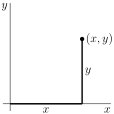
\includegraphics[width=\linewidth]{figs/point2d}
\end{sbspanel}%
\end{sidebyside}%
\par
The set of all points in two dimensions is denoted\footnote{Not surprisingly, the \(2\) in \(\bbbr^2\) signifies that each point is labelled by two numbers and the \(\bbbr\) in \(\bbbr^2\) signifies that the numbers in question are real numbers. There are more advanced applications (for example in signal analysis and in quantum mechanics) where complex numbers are used. The space of all pairs \((z_1,z_2)\), with \(z_1\) and \(z_2\) complex numbers is denoted  \(\bbbc^2\).\label{g:fn:idm45408056016368}} \(\bbbr^2\). Observe that%
\begin{itemize}[label=\textbullet]
\item{}the distance from the point \((x,y)\) to the \(x\)-axis is \(|y|\)%
\item{}if \(y\gt 0\), then \((x,y)\) is above the \(x\)-axis and if \(y\lt 0\), then \((x,y)\) is below the \(x\)-axis%
\item{}the distance from the point \((x,y)\) to the \(y\)-axis is \(|x|\)%
\item{}if \(x\gt 0\), then \((x,y)\) is to the right of the \(y\)-axis and if \(x\lt 0\), then \((x,y)\) is to the left of the \(y\)-axis%
\item{}the distance from the point \((x,y)\) to the origin \((0,0)\) is \(\sqrt{x^2+y^2}\)%
\end{itemize}
Similarly, each point in three dimensions may be labeled by three coordinates \((x,y,z)\), as in the two figures below.%
\begin{sidebyside}{2}{0.085}{0.085}{0.17}%
\begin{sbspanel}{0.33}%
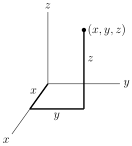
\includegraphics[width=\linewidth]{figs/point3d}
\end{sbspanel}%
\begin{sbspanel}{0.33}%
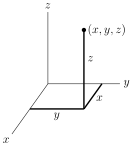
\includegraphics[width=\linewidth]{figs/point3db}
\end{sbspanel}%
\end{sidebyside}%
\par
The set of all points in three dimensions is denoted \(\bbbr^3\). The plane that contains, for example, the \(x\)- and \(y\)-axes is called the \(xy\)-plane.%
\begin{itemize}[label=\textbullet]
\item{}The \(xy\)-plane is the set of all points \((x,y,z)\) that satisfy \(z=0\).%
\item{}The \(xz\)-plane is the set of all points \((x,y,z)\) that satisfy \(y=0\).%
\item{}The \(yz\)-plane is the set of all points \((x,y,z)\) that satisfy \(x=0\).%
\end{itemize}
More generally,%
\begin{itemize}[label=\textbullet]
\item{}The set of all points \((x,y,z)\) that obey \(z=c\) is a plane that is parallel to the \(xy\)-plane and is a distance \(|c|\) from it. If \(c \gt 0\), the plane \(z=c\) is above the \(xy\)-plane. If \(c \lt 0\), the plane \(z=c\) is below the \(xy\)-plane. We say that the plane \(z=c\) is a signed distance \(c\) from the \(xy\)-plane.%
\item{}The set of all points \((x,y,z)\) that obey \(y=b\) is a plane that is parallel to the \(xz\)-plane and is a signed distance \(b\) from it.%
\item{}The set of all points \((x,y,z)\) that obey \(x=a\) is a plane that is parallel to the \(yz\)-plane and is a signed distance \(a\) from it.%
\end{itemize}
%
\begin{sidebyside}{3}{0}{0}{0}%
\begin{sbspanel}{0.333333333333333}%
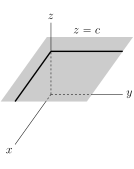
\includegraphics[width=\linewidth]{figs/xyplaneN}
\end{sbspanel}%
\begin{sbspanel}{0.333333333333333}%
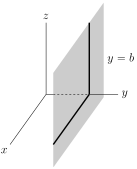
\includegraphics[width=\linewidth]{figs/xzplaneN}
\end{sbspanel}%
\begin{sbspanel}{0.333333333333333}%
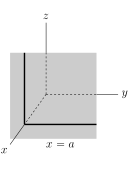
\includegraphics[width=\linewidth]{figs/yzplaneN}
\end{sbspanel}%
\end{sidebyside}%
\par
Observe that our 2d distances extend quite easily to 3d.%
\begin{itemize}[label=\textbullet]
\item{}the distance from the point \((x,y,z)\) to the \(xy\)-plane is \(|z|\)%
\item{}the distance from the point \((x,y,z)\) to the \(xz\)-plane is \(|y|\)%
\item{}the distance from the point \((x,y,z)\) to the \(yz\)-plane is \(|x|\)%
\item{}the distance from the point \((x,y,z)\) to the origin \((0,0,0)\) is \(\sqrt{x^2+y^2+z^2}\)%
\end{itemize}
To see that the distance from the point \((x,y,z)\) to the origin \((0,0,0)\) is indeed  \(\sqrt{x^2+y^2+z^2}\),%
\begin{itemize}[label=\textbullet]
\item{}apply Pythagoras to the right-angled triangle with vertices \((0,0,0)\), \((x,0,0)\) and \((x,y,0)\) to see that the distance from \((0,0,0)\) to \((x,y,0)\) is \(\sqrt{x^2+y^2}\) and then%
\item{}apply Pythagoras to the right-angled triangle with vertices \((0,0,0)\), \((x,y,0)\) and \((x,y,z)\) to see that the distance from \((0,0,0)\) to \((x,y,z)\) is \(\sqrt{{\big(\sqrt{x^2+y^2}\big)}^2+z^2}
=\sqrt{x^2+y^2+z^2}\).%
\end{itemize}
%
\begin{sidebyside}{1}{0.3}{0.3}{0}%
\begin{sbspanel}{0.4}%
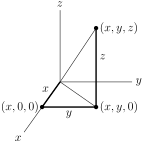
\includegraphics[width=\linewidth]{figs/pythag3d}
\end{sbspanel}%
\end{sidebyside}%
\par
More generally, the distance from the point \((x,y,z)\) to the point \((x',y',z')\) is%
\begin{equation*}
\sqrt{(x-x')^2+(y-y')^2+(z-z')^2}
\end{equation*}
Notice that this gives us the equation for a sphere quite directly. All the points on a sphere are equidistant from the centre of the sphere. So, for example, the equation of the sphere centered on \((1,2,3)\) with radius \(4\), that is, the set of all points \((x,y,z)\) whose distance from \((1,2,3)\) is \(4\), is%
\begin{equation*}
(x-1)^2+(y-2)^2+(z-3)^2=16
\end{equation*}
%
\par
Here is an example in which we sketch a region in the \(xy\)-plane that is specified using inequalities.%
\begin{example}{}{g:example:idm45408045487856}%
In this example, we sketch the region%
\begin{equation*}
\Set{(x,y)}{ -12\le x^2-6x +y^2-4y \le -9,\ \ y\ge 1}
\end{equation*}
in the \(xy\)-plane.%
\par
We do so in two steps. In the first step, we sketch the curves \(x^2-6x +y^2-4y=-12\), \(x^2-6x +y^2-4y=-9\), and \(y=1\).%
\begin{itemize}[label=\textbullet]
\item{}By completing squares, we see that the equation  \(x^2-6x +y^2-4y=-12\) is equivalent to \((x-3)^2 +(y-2)^2 =1\), which is the circle of radius \(1\) centred on \((3,2)\). It is sketched in the figure below.%
\item{}By completing squares, we see that the equation  \(x^2-6x +y^2-4y=-9\) is equivalent to \((x-3)^2 +(y-2)^2 =4\), which is the circle of radius \(2\) centred on \((3,2)\). It is sketched in the figure below.%
\item{}The point \((x,y)\) obeys \(y=1\) if and only if it is a distance \(1\) vertically above the \(x\)-axis. So \(y=1\) is the line that is parallel to the \(x\)-axis and is one unit above it. This line is also  sketched in the figure below.%
\end{itemize}
%
\begin{sidebyside}{1}{0.185}{0.185}{0}%
\begin{sbspanel}{0.63}%
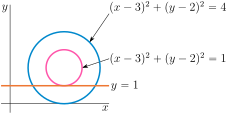
\includegraphics[width=\linewidth]{figs/annulusPart}
\end{sbspanel}%
\end{sidebyside}%
\par
In the second step we determine the impact that the inequalities have.%
\begin{itemize}[label=\textbullet]
\item{}The inequality \(x^2-6x +y^2-4y\ge -12\) is equivalent to \((x-3)^2 +(y-2)^2 \ge 1\) and hence is equivalent to \(\sqrt{(x-3)^2 +(y-2)^2} \ge 1\). So the point \((x,y)\) satisfies \(x^2-6x +y^2-4y\ge -12\) if and only if the distance from \((x,y)\) to \((3,2)\) is at least \(1\), i.e. if and only if \((x,y)\) is outside (or on) the circle \((x-3)^2 +(y-2)^2 = 1\).%
\item{}The inequality \(x^2-6x +y^2-4y\le -9\) is equivalent to \((x-3)^2 +(y-2)^2 \le 4\) and hence is equivalent to \(\sqrt{(x-3)^2 +(y-2)^2} \le 2\). So the point \((x,y)\) satisfies the inequality \(x^2-6x +y^2-4y\le -9\) if and only if the distance from \((x,y)\) to \((3,2)\) is at most \(2\), i.e. if and only if \((x,y)\) is inside (or on) the circle \((x-3)^2 +(y-2)^2 = 4\).%
\item{}The point \((x,y)\) obeys \(y\ge 1\) if and only if \((x,y)\) is a vertical distance at least \(1\) above the \(x\)-axis, i.e. is above (or on) the line \(y=1\).%
\item{}So the region%
\begin{equation*}
\Set{(x,y)}{ -12\le x^2-6x +y^2-4y \le -9,\ \ y\ge 1}
\end{equation*}
consists of all points \((x,y)\) that%
\begin{itemize}[label=$\circ$]
\item{}are inside or on the circle \((x-3)^2 +(y-2)^2 = 4\) and%
\item{}are also outside or on the circle \((x-3)^2 +(y-2)^2 = 1\) and%
\item{}are also above or on the line \(y=1\).%
\end{itemize}
It is the shaded region in the figure below.%
\end{itemize}
%
\begin{sidebyside}{1}{0.185}{0.185}{0}%
\begin{sbspanel}{0.63}%
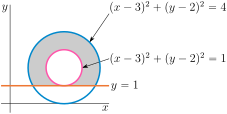
\includegraphics[width=\linewidth]{figs/annulusPartB}
\end{sbspanel}%
\end{sidebyside}%
\end{example}
Here are a couple of examples that involve spheres.%
\begin{example}{}{g:example:idm45408052716288}%
In this example, we are going to find the curve formed by the intersection of the \(xy\)-plane and the sphere of radius \(5\) centred on \((0,0,4)\).%
\par
The point \((x,y,z)\) lies on the \(xy\)-plane if and only if \(z=0\), and lies on the sphere of radius \(5\) centred on \((0,0,4)\) if and only if \(x^2+y^2+(z-4)^2=25\). So the point \((x,y,z)\) lies on the curve of intersection if and only if both \(z=0\) and \(x^2+y^2+(z-4)^2=25\), or equivalently%
\begin{equation*}
z=0,\quad x^2+y^2+(0-4)^2=25
\iff
z=0,\quad x^2+y^2 = 9
\end{equation*}
This is the circle in the \(xy\)-plane that is centred on the origin and has radius \(3\). Here is a sketch that show the parts of the sphere and the circle of intersection that are in the first octant. That is, that have \(x\ge 0\), \(y\ge 0\) and \(z\ge 0\).%
\begin{sidebyside}{1}{0.33}{0.33}{0}%
\begin{sbspanel}{0.34}%
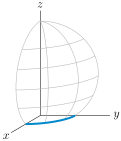
\includegraphics[width=\linewidth]{figs/sphereCircle}
\end{sbspanel}%
\end{sidebyside}%
\end{example}
\begin{example}{}{g:example:idm45408046675600}%
In this example, we are going to find all points \((x,y,z)\) for which the distance from \((x,y,z)\) to \((9,-12,15)\) is twice the distance from \((x,y,z)\) to the origin \((0,0,0)\).%
\par
The distance from \((x,y,z)\) to \((9,-12,15)\) is \(\sqrt{(x-9)^2+(y+12)^2+(z-15)^2}\). The distance from \((x,y,z)\) to \((0,0,0)\) is \(\sqrt{x^2+y^2+z^2}\). So we want to find all points \((x,y,z)\) for which%
\begin{equation*}
\sqrt{(x-9)^2+(y+12)^2+(z-15)^2}
=2\sqrt{x^2+y^2+z^2}
\end{equation*}
Squaring both sides of this equation gives%
\begin{equation*}
x^2-18x+81 +y^2+24y+144 +z^2-30z+225 = 4\big(x^2+y^2+z^2)
\end{equation*}
Collecting up terms gives%
\begin{alignat*}{1}
3x^2+18x +3y^2-24y +3z^2+30z \amp= 450\ \text{and, dividing by 3,} \\
x^2+6x +y^2-8y +z^2+10z \amp= 150\ \text{and, completing squares,}\\
x^2+6x +9 +y^2-8y +16  +z^2+10z +25 \amp= 200\ \text{or}\\
(x+3)^2+(y-4)^2+(z+5)^2 \amp=200 
\end{alignat*}
This is the sphere of radius \(10\sqrt{2}\) centred on \((-3,4,-5)\).%
\end{example}
%
%
\typeout{************************************************}
\typeout{Exercises 1.1.1 Exercises}
\typeout{************************************************}
%
\begin{exercises-subsection}{Exercises}{}{Exercises}{}{}{g:exercises:idm45408056758192}
\par\medskip\noindent%
%
\alert{Exercises — Stage 1}%
\begin{exercisegroup}
\begin{divisionexerciseeg}{1}{}{}{g:exercise:idm45408056608512}%
Describe the set of all points \((x,y,z)\) in \(\bbbr^3\) that satisfy%
\begin{enumerate}[label=\alph*]
\item{}\(\displaystyle x^2 +y^2+z^2= 2x-4y+4\)%
\item{}\(\displaystyle x^2 +y^2+z^2 \lt  2x-4y+4\)%
\end{enumerate}
%
\end{divisionexerciseeg}%
\begin{divisionexerciseeg}{2}{}{}{g:exercise:idm45408054739856}%
Describe and sketch the set of all points \((x,y)\) in \(\bbbr^2\) that satisfy%
\begin{enumerate}[label=\alph*]
\item{}\(\displaystyle x=y\)%
\item{}\(\displaystyle x+y=1\)%
\item{}\(\displaystyle x^2+y^2=4\)%
\item{}\(\displaystyle x^2+y^2=2y\)%
\item{}\(\displaystyle x^2+y^2 \lt 2y\)%
\end{enumerate}
%
\end{divisionexerciseeg}%
\begin{divisionexerciseeg}{3}{}{}{g:exercise:idm45408059336816}%
Describe the set of all points \((x,y,z)\) in \(\bbbr^3\) that satisfy the following conditions. Sketch the part of the set that is in the first octant.%
\begin{enumerate}[label=\alph*]
\item{}\(\displaystyle z = x\)%
\item{}\(\displaystyle x + y + z = 1\)%
\item{}\(\displaystyle x^2 + y^2 + z^2 = 4\)%
\item{}\(x^2 + y^2 + z^2 = 4\), \(z = 1\)%
\item{}\(\displaystyle x^2+y^2=4\)%
\item{}\(\displaystyle z = x^2 + y^2\)%
\end{enumerate}
%
\end{divisionexerciseeg}%
\begin{divisionexerciseeg}{4}{}{}{g:exercise:idm45408032195376}%
Let \(A\) be the point \((2,1,3)\).%
\begin{enumerate}[label=\alph*]
\item{}Find the distance from \(A\) to the \(xy\)-plane.%
\item{}Find the distance from \(A\) to the \(xz\)-plane.%
\item{}Find the distance from \(A\) to the point \((x,0,0)\) on the \(x\)-axis.%
\item{}Find the point on the \(x\)-axis that is closest to \(A\).%
\item{}What is the distance from \(A\) to the \(x\)-axis?%
\end{enumerate}
%
\end{divisionexerciseeg}%
\end{exercisegroup}
\par\medskip\noindent
\par\medskip\noindent%
%
\alert{Exercises — Stage 2}%
\begin{exercisegroup}
\begin{divisionexerciseeg}{5}{}{}{g:exercise:idm45408032455008}%
Consider any triangle. Pick a coordinate system so that one vertex is at the origin and a second vertex is on the positive \(x\)-axis. Call the coordinates of the second vertex \((a,0)\) and those of the third vertex \((b,c)\). Find the circumscribing circle (the circle that goes through all three vertices).%
\end{divisionexerciseeg}%
\begin{divisionexerciseeg}{6}{\(\ast\).}{}{g:exercise:idm45408032558048}%
A certain surface consists of all points \(P=(x,y,z)\) such that the distance from \(P\) to the point \((0,0,1)\) is equal to the distance from \(P\) to the plane \(z+1=0\). Find an equation for the surface, sketch and describe it verbally.%
\end{divisionexerciseeg}%
\begin{divisionexerciseeg}{7}{}{}{g:exercise:idm45408032646064}%
Show that the set of all points \(P\) that are twice as far from \((3,-2,3)\) as from \((3/2,1,0)\) is a sphere. Find its centre and radius.%
\end{divisionexerciseeg}%
\end{exercisegroup}
\par\medskip\noindent
\par\medskip\noindent%
%
\alert{Exercises — Stage 3}%
\begin{exercisegroup}
\begin{divisionexerciseeg}{8}{}{}{g:exercise:idm45408032775488}%
The pressure \(p(x,y)\) at the point \((x,y)\)  is at least zero and is determined by the equation \(x^2-2px+y^2=3p^2\). Sketch several isobars. An isobar is a curve with equation \(p(x,y)=c\) for some constant \(c\ge 0\).%
\end{divisionexerciseeg}%
\end{exercisegroup}
\par\medskip\noindent
\end{exercises-subsection}
\end{sectionptx}
%
%
\typeout{************************************************}
\typeout{Section 1.2 Vectors}
\typeout{************************************************}
%
\begin{sectionptx}{Vectors}{}{Vectors}{}{}{x:section:sec_vectors}
\begin{introduction}{}%
In many of our applications in 2d and 3d, we will encounter quantities that have both a magnitude (like a distance) and also a direction. Such quantities are called vectors. That is, a \emph{vector} is a quantity which has both a direction and a magnitude, like a velocity. If you are moving, the magnitude (length) of your velocity vector is your speed (distance travelled per unit time)  and the direction of your velocity vector is your direction of motion. To specify a vector in three dimensions you have to give three components, just as for a point. To draw the vector with components \(a, b, c \) you can draw an arrow from the point \((0,0,0)\) to the point \((a,b,c)\).%
\begin{sidebyside}{2}{0.085}{0.085}{0.17}%
\begin{sbspanel}{0.33}%
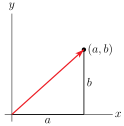
\includegraphics[width=\linewidth]{figs/vector2d}
\end{sbspanel}%
\begin{sbspanel}{0.33}%
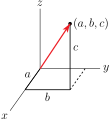
\includegraphics[width=\linewidth]{figs/vector3d}
\end{sbspanel}%
\end{sidebyside}%
\par
Similarly, to specify a vector in two dimensions you have to give two components and to draw the vector with components \(a, b \) you can draw an arrow from the point \((0,0)\) to the point \((a,b)\).%
\par
There are many situations in which it is preferable to draw a vector with its tail at some point other than the origin. For example, it is natural to draw the velocity vector of a moving particle with the tail of the velocity vector at the position of the particle, whether or not the particle is at the origin. The sketch below shows a moving particle and its velocity vector at two different times.%
\begin{sidebyside}{1}{0.355}{0.355}{0}%
\begin{sbspanel}{0.29}%
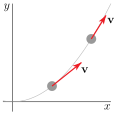
\includegraphics[width=\linewidth]{figs/movingParticle}
\end{sbspanel}%
\end{sidebyside}%
\par
As a second example, suppose that you are analyzing the motion of a pendulum. There are three forces acting on the pendulum bob: gravity \(\vg\), which is pulling the bob straight down, tension \(\vt\) in the rod, which is pulling the bob in the direction of the rod, and air resistance \(\vr\), which is pulling the bob in a direction opposite to its direction of motion. All three forces are acting on the bob. So it is natural to draw all three arrows representing the forces with their tails at the bob.%
\begin{sidebyside}{1}{0.4}{0.4}{0}%
\begin{sbspanel}{0.2}%
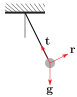
\includegraphics[width=\linewidth]{figs/pendulum}
\end{sbspanel}%
\end{sidebyside}%
\par
In this text, we will used bold faced letters, like \(\vv\), \(\vt\), \(\vg\), to designate vectors. In handwriting, it is clearer to use a small overhead arrow\footnote{Some people use an underline, as in \(\underline{v}\), rather than an arrow.\label{g:fn:idm45408033003648}}, as in \(\vec{v}\), \(\vec{t}\), \(\vec{g}\), instead. Also, when we want to emphasise that some quantity is a number, rather than a vector, we will call the number a \emph{scalar}.%
\par
Both points and vectors in 2d are specified by two numbers. Until you get used to this, it might confuse you sometimes \textemdash{} does a given pair of numbers represent a point or a vector? To distinguish\footnote{Or, in the Wikipedia jargon, disambiguate.\label{g:fn:idm45408033035648}} between the components of a vector and the coordinates of the point at its head, when its tail is at some point other than the origin, we shall use angle brackets rather than round brackets around the components of a vector. For example, the figure below shows the two-dimensional vector \(\llt 2,1\rgt\) drawn in three different positions. In each case, when the tail is at the point \((u,v)\) the head is at \((2+u,1+v)\). We warn you that, out in the  real world\footnote{OK. OK. Out in that (admittedly very small) part of the real world that actually knows what a vector is.\label{g:fn:idm45408033056608}}, no one uses notation that distinguishes between components of a vector and the coordinates of its head \textemdash{} usually round brackets are used for both. It is up to you to keep straight which is being referred to.%
\begin{sidebyside}{1}{0.2}{0.2}{0}%
\begin{sbspanel}{0.6}%
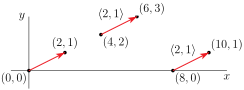
\includegraphics[width=\linewidth]{figs/positions}
\end{sbspanel}%
\end{sidebyside}%
\par
By way of summary,%
\begin{definition}{}{x:definition:not_scalar_vector}%
we use%
\begin{itemize}[label=\textbullet]
\item{}bold faced letters, like \(\vv\), \(\vt\), \(\vg\), to designate vectors, and%
\item{}angle brackets, like \(\llt 2,1\rgt\), around the components of a vector, but use%
\item{}round brackets, like \((2,1)\), around the coordinates of a point, and use%
\item{}``scalar'' to emphasise that some quantity is a number, rather than a vector.%
\end{itemize}
%
\end{definition}
\end{introduction}%
%
%
\typeout{************************************************}
\typeout{Subsection 1.2.1 Addition of Vectors and Multiplication of a Vector by a Scalar}
\typeout{************************************************}
%
\begin{subsectionptx}{Addition of Vectors and Multiplication of a Vector by a Scalar}{}{Addition of Vectors and Multiplication of a Vector by a Scalar}{}{}{x:subsection:subsec-addvec}
Just as we have done many times in the CLP texts, when we define a new type of object, we want to understand how it interacts with the basic operations of addition and multiplication. Vectors are no different, and we shall shortly see a natural way to define addition of vectors. Multiplication will be more subtle, and we shall start with multiplication of a vector by a number (rather than with multiplication of a vector by another vector).%
\par
By way of motivation for the definitions of addition and multiplication by a number, imagine that we are out for a walk on the \(xy\)-plane.%
\begin{itemize}[label=\textbullet]
\item{}Suppose that we take a step and, in doing so, we move \(a_1\) units parallel to the \(x\)-axis and \(a_2\) units parallel to the \(y\)-axis. Then we say that \(\llt a_1, a_2\rgt\) is the displacement vector for the step. Suppose now that we take a second step which moves us an additional \(b_1\) units  parallel to the \(x\)-axis and an additional \(b_2\) units  parallel to the \(y\)-axis, as in the figure on the left below. So the displacement vector for the second step is \(\llt b_1, b_2\rgt\). All together, we have moved \(a_1+b_1\) units  parallel to the \(x\)-axis and \(a_2+b_2\) units parallel to the \(y\)-axis. The displacement vector for the two steps combined is \(\llt a_1+b_1, a_2+b_2\rgt\). We shall define the sum of \(\llt a_1, a_2\rgt\) and \(\llt b_1, b_2\rgt\), denoted by \(\llt a_1, a_2\rgt+\llt b_1,b_2\rgt\), to be \(\llt a_1+b_1, a_2+b_2\rgt\).%
\item{}Suppose now that, instead, we decide to step in the same direction as the first step above, but to move twice as far, as in the figure on the right below. That is, our step will move us \(2a_1\) units in the direction of the \(x\)-axis and \(2a_2\) units in the direction of the \(y\)-axis and the corresponding displacement vector will be \(\llt 2a_1, 2a_2\rgt\). We shall define the product of the number \(2\) and the vector \(\llt a_1, a_2\rgt\), denoted by \(2\llt a_1, a_2\rgt\), to be \(\llt 2a_1, 2a_2\rgt\).%
\end{itemize}
%
\begin{sidebyside}{2}{0.057}{0.057}{0.114}%
\begin{sbspanel}{0.394}[center]%
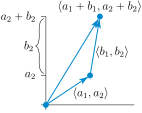
\includegraphics[width=\linewidth]{figs/maddvec}
\end{sbspanel}%
\begin{sbspanel}{0.378}[center]%
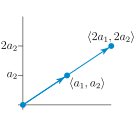
\includegraphics[width=\linewidth]{figs/mscalmul}
\end{sbspanel}%
\end{sidebyside}%
\par
Here are the formal definitions.%
\begin{definition}{Adding Vectors and Multiplying a Vector by a Number.}{x:definition:def_addScalMult}%
These two operations have the obvious definitions%
\begin{align*}
\va=\llt a_1,a_2\rgt,\ \vb =\llt b_1,b_2\rgt
\amp\amp
\implies\amp\amp \va+\vb=\llt a_1+b_1,a_2+b_2\rgt\\
\va=\llt a_1,a_2\rgt,\ s\text{ a number}
\amp\amp
\implies\amp\amp s\va=\llt sa_1,sa_2\rgt
\end{align*}
and similarly in three dimensions.%
\end{definition}
Pictorially, you add the vector \(\vb\) to the vector \(\va\) by drawing \(\vb\) with its tail at the head of \(\va\) and then drawing a vector from the tail of \(\va\) to the head of \(\vb\), as in the figure on the left below. For a number \(s\), we can draw the vector \(s\va\), by just%
\begin{itemize}[label=\textbullet]
\item{}changing the vector \(\va\)'s length by the factor \(|s|\), and,%
\item{}if \(s \lt 0\), reversing the arrow's direction,%
\end{itemize}
as in the other two figures below.%
\begin{sidebyside}{3}{0.0283333333333333}{0.0283333333333333}{0.0566666666666667}%
\begin{sbspanel}{0.33}[center]%
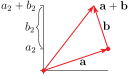
\includegraphics[width=\linewidth]{figs/addvec}
\end{sbspanel}%
\begin{sbspanel}{0.25}[center]%
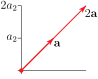
\includegraphics[width=\linewidth]{figs/scalmul}
\end{sbspanel}%
\begin{sbspanel}{0.25}[center]%
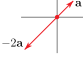
\includegraphics[width=\linewidth]{figs/negmul}
\end{sbspanel}%
\end{sidebyside}%
\par
The special case of multiplication by \(s=-1\) appears so frequently that \((-1)\va\) is given the shorter notation \(-\va\). That is,%
\begin{equation*}
-\llt a_1,a_2\rgt=\llt -a_1,-a_2\rgt
\end{equation*}
Of course \(\va+(-\va)\) is \(\vZero\), the vector all of whose components are zero.%
\par
To subtract \(\vb\) from \(\va\) pictorially, you may add \(-\vb\) (which is drawn by reversing the direction of \(\vb\)) to \(\va\). Alternatively, if you draw \(\va\) and \(\vb\) with their tails at a common point, then \(\va-\vb\) is the vector from the head of \(\vb\) to the head of \(\va\). That is, \(\va-\vb\) is the vector you must add to \(\vb\) in order to get \(\va\).%
\begin{sidebyside}{1}{0.3}{0.3}{0}%
\begin{sbspanel}{0.4}%
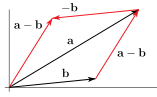
\includegraphics[width=\linewidth]{figs/subtract}
\end{sbspanel}%
\end{sidebyside}%
\par
The operations of addition and multiplication by a scalar that we have just defined are quite natural and rarely cause any problems, because they inherit from the real numbers the properties of  addition and multiplication that you are used to.%
\begin{theorem}{Properties of Addition and Scalar Multiplication.}{}{x:theorem:thm_addScalMult}%
Let \(\va\), \(\vb\) and \(\vc\) be vectors and \(s\) and \(t\) be scalars. Then%
\begin{alignat*}{4}
& (1)\quad&&\va+\vb=\vb+\va \qquad\qquad\qquad
&& (2)\quad&&\va+(\vb+\vc)=(\va+\vb)+\vc\\
& (3) &&\va+\vZero =\va
&& (4) &&\va+(-\va)=\vZero\\
& (5) &&s(\va+\vb)=s\va+s\vb
&& (6) &&(s+t)\va=s\va+t\va\\
& (7) &&(st)\va = s(t\va)
&& (8) &&1\va=\va
\end{alignat*}
%
\end{theorem}
We have just been introduced to many definitions. Let's see some of them in action.%
\begin{example}{}{g:example:idm45408033593264}%
For example, if%
\begin{equation*}
\va = \llt 1,2,3\rgt\qquad
\vb = \llt 3,2,1\rgt\qquad
\vc = \llt 1,0,1\rgt
\end{equation*}
then%
\begin{alignat*}{2}
2\va&=2\llt 1,2,3\rgt&&=\llt 2,4,6\rgt\\
-\vb&=-\llt 3,2,1\rgt&&=\llt -3,-2,-1\rgt\\
3\vc&=3\llt 1,0,1\rgt&&=\llt 3,0,3\rgt
\end{alignat*}
and%
\begin{align*}
2\va-\vb+3\vc
&= \llt 2,4,6\rgt + \llt -3,-2,-1\rgt+\llt 3,0,3\rgt\\
&= \llt 2-3+3\,,\,4-2+0\,,\,6-1+3\rgt\\
&= \llt 2,2,8 \rgt
\end{align*}
%
\end{example}
\begin{definition}{}{x:definition:def_parallel_vectors}%
Two vectors \(\va\) and \(\vb\)%
\begin{itemize}[label=\textbullet]
\item{}are said to be parallel if \(\ \va= s\,\vb\ \) for some nonzero real number \(s\) and%
\item{}are said to have the same direction if \(\ \va=s\,\vb\ \) for some number \(s \gt 0\).%
\end{itemize}
%
\end{definition}
There are some vectors that occur sufficiently commonly that they are given special names. One is the vector \(\vZero\). Some others are the ``standard basis vectors''.%
\begin{definition}{}{x:definition:def_basis_vectors}%
The standard basis vectors in two dimensions are%
\begin{equation*}
\hi = \llt 1,0\rgt \qquad\qquad\hj =\llt 0,1\rgt
\end{equation*}
%
\begin{sidebyside}{1}{0.425}{0.425}{0}%
\begin{sbspanel}{0.15}%
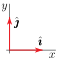
\includegraphics[width=\linewidth]{figs/basis2d}
\end{sbspanel}%
\end{sidebyside}%
\par
The standard basis vectors in three dimensions are%
\begin{equation*}
\hi = \llt 1,0,0\rgt \qquad\qquad\hj =\llt 0,1,0\rgt
\qquad\qquad\hk =\llt 0,0,1\rgt
\end{equation*}
%
\begin{sidebyside}{1}{0.375}{0.375}{0}%
\begin{sbspanel}{0.25}%
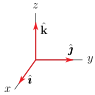
\includegraphics[width=\linewidth]{figs/basis3d}
\end{sbspanel}%
\end{sidebyside}%
\end{definition}
We'll explain the little hats in the notation \(\hi\), \(\hj\), \(\hk\) shortly. Some people rename \(\hi\), \(\hj\) and \(\hk\) to \(\he_1\), \(\he_2\) and \(\he_3\) respectively. Using the above properties we have, for all vectors,%
\begin{equation*}
\llt a_1,a_2\rgt =a_1\,\hi+a_2\,\hj\qquad\qquad
\llt a_1,a_2,a_3\rgt =a_1\,\hi+a_2\,\hj+a_3\,\hk
\end{equation*}
A sum of numbers times vectors, like \(a_1\hi+a_2\hj\) is called a linear combination of the vectors. Thus all vectors can be expressed as linear combinations of the standard basis vectors. This makes basis vectors very helpful in computations. The  standard basis vectors are unit vectors, meaning that they are of length one, where the length of a vector \(\va\) is denoted\footnote{The notation \(\|\va\|\) is also used for the length of \(\va\).\label{g:fn:idm45408033808704}} \(|\va|\) and is defined by%
\begin{definition}{Length of a Vector.}{x:definition:def_vectLen}%
%
\begin{alignat*}{3}
&\va=\llt a_1,a_2\rgt \qquad&&\implies\qquad &&|\va|=\sqrt{a_1^2+a_2^2}\\
&\va=\llt a_1,a_2,a_3\rgt \qquad&&\implies\qquad &&|\va|=\sqrt{a_1^2+a_2^2+a_3^2}
\end{alignat*}
A unit vector is a vector of length one. We'll sometimes use the accent \(\hat{\ }\) to emphasise that the vector \(\hat\va\) is a unit vector. That is, \(|\hat\va|=1\).%
\end{definition}
\begin{example}{}{x:example:eg_unit_vector}%
Recall that multiplying a vector \(\va\) by a positive number \(s\), changes the length of the vector by a factor \(s\) without changing the direction of the vector. So (assuming that \(|\va|\ne 0)\) \(\frac{\va}{|\va|}\) is a unit vector that has the same direction as \(\va\). For example, \(\frac{\llt 1,1,1\rgt}{\sqrt{3}}\) is a unit vector that points in the same direction as \(\llt 1,1,1\rgt\).%
\end{example}
\begin{example}{}{x:example:eg_walk}%
We go for a walk on a flat Earth. We use a coordinate system with the positive x-axis pointing due east and the positive y-axis pointing due north. We%
\begin{itemize}[label=\textbullet]
\item{}start at the origin and%
\item{}walk due east for 4 units and then%
\item{}walk northeast for \(5\sqrt{2}\) units and then%
\item{}head towards the point \((0,11)\), but we only go%
\item{}one third of the way.%
\end{itemize}
%
\begin{sidebyside}{2}{0.075}{0.075}{0.15}%
\begin{sbspanel}{0.5}[center]%
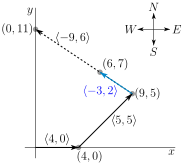
\includegraphics[width=\linewidth]{figs/addSubtractMult}
\end{sbspanel}%
\begin{sbspanel}{0.2}[center]%
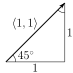
\includegraphics[width=\linewidth]{figs/triangleWalk}
\end{sbspanel}%
\end{sidebyside}%
\par
We will now use vectors to figure out our final location.%
\begin{itemize}[label=\textbullet]
\item{}On the first leg of our walk, we go 4 units in the positive \(x\)-direction. So our displacement vector \textemdash{} the vector whose tail is at our starting point and whose head is at the end point of the first leg \textemdash{} is \(\llt 4,0\rgt\). As we started at \((0,0)\) we finish the first leg of the walk at \((4,0)\).%
\item{}On the second leg of our walk, our direction of motion is northeast, i.e. is \(45^\circ\) above the direction of the positive \(x\)-axis. Looking at the figure on the right above, we see that our displacement vector, for the second leg of the walk, has to be in the same direction as the vector \(\llt 1,1\rgt\). So our displacement vector is the vector of length \(5\sqrt{2}\) with the same direction as \(\llt 1,1\rgt\). The vector \(\llt 1,1\rgt\) has length \(\sqrt{1^2+1^2}=\sqrt{2}\) and so \(\frac{\llt 1,1\rgt}{\sqrt{2}}\) has length one and our displacement vector is%
\begin{equation*}
5\sqrt{2}\ \frac{\llt 1,1\rgt}{\sqrt{2}}
=5 \llt 1,1\rgt
=\llt 5,5\rgt
\end{equation*}
If we draw this displacement vector, \(\llt 5,5\rgt\) with its tail at \((4,0)\), the starting point of the second leg of the walk, then its head will be at \((4+5, 0+5)=(9,5)\) and that is the end point of the second leg of the walk.%
\item{}On the final leg of our walk, we start at \((9,5)\) and walk towards \((0,11)\). The vector from \((9,5)\) to \((0,11)\) is \(\llt 0-9\,,\,11-5\rgt =\llt -9,6\rgt\). As we go only one third of the way, our final displacement vector is%
\begin{equation*}
\frac{1}{3}\llt -9,6\rgt
=\llt -3,2\rgt
\end{equation*}
If we draw this displacement vector with its tail at \((9,5)\), the starting point of the final leg, then its head will be at \((9-3, 5+2)=(6,7)\) and that is the end point of the final leg of the walk, and our final location.%
\end{itemize}
%
\end{example}
\end{subsectionptx}
%
%
\typeout{************************************************}
\typeout{Subsection 1.2.2 The Dot Product}
\typeout{************************************************}
%
\begin{subsectionptx}{The Dot Product}{}{The Dot Product}{}{}{x:subsection:subsec-dotprod}
Let's get back to the arithmetic operations of addition and multiplication. We will be using both scalars and vectors. So, for each operation there are three possibilities that we need to explore:%
\begin{itemize}[label=\textbullet]
\item{}``scalar plus scalar'', ``scalar plus vector'' and ``vector plus vector''%
\item{}``scalar times scalar'', ``scalar times vector'' and ``vector times vector''%
\end{itemize}
We have been using ``scalar plus scalar'' and ``scalar times scalar'' since childhood. ``vector plus vector'' and ``scalar times vector'' were just defined above. There is no sensible way to define ``scalar plus vector'', so we won't. This leaves ``vector times vector''. There are actually two widely used such products. The first is the \emph{dot product}, which is the topic of this section, and which is used to easily determine the angle \(\theta\) (or more precisely, \(\cos\theta\)) between two vectors. We'll get to the second, the cross product, later.%
\par
Here is preview of what we will do in this dot product subsection §\hyperref[x:subsection:subsec-dotprod]{{\xreffont\ref{x:subsection:subsec-dotprod}}}. We are going to give two formulae for the dot product, \(\va\cdot\vb\), of the pair of vectors \(\va=\llt a_1,a_2,a_3\rgt\) and \(\vb=\llt b_1,b_2,b_3\rgt\).%
\begin{itemize}[label=\textbullet]
\item{}The first formula is \(\va\cdot\vb = a_1b_1+a_2b_2+a_3b_3\). We will take it as our official definition of \(\va\cdot\vb\). This formula provides us with an easy way to compute dot products.%
\item{}The second formula is \(\va\cdot\vb=|\va|\,|\vb|\,\cos\theta\), where \(\theta\) is the angle between \(\va\) and \(\vb\).%
\begin{sidebyside}{1}{0.4235}{0.4235}{0}%
\begin{sbspanel}{0.153}%
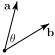
\includegraphics[width=\linewidth]{figs/dotAngle}
\end{sbspanel}%
\end{sidebyside}%
\par
We will show, in Theorem \hyperref[x:theorem:thm_dotPppties]{{\xreffont\ref{x:theorem:thm_dotPppties}}} below, that this second formula always gives the same answer as the first formula. The second formula provides us with an easy way to determine the angle between two vectors. In particular, it provides us with an easy way to test whether or not two vectors are perpendicular to each other. For example, the vectors \(\llt 1,2,3\rgt\) and \(\llt -1,-1,1\rgt\) have dot product%
\begin{equation*}
\llt 1,2,3\rgt\cdot\llt -1,-1,1\rgt = 1\times(-1)+2\times(-1)+3\times 1=0
\end{equation*}
This tell us as the angle \(\theta\) between the two vectors obeys \(\cos\theta=0\), so that \(\theta=\frac{\pi}{2}\). That is, the two vectors are perpendicular to each other.%
\end{itemize}
After we give our official definition of the dot product in Definition \hyperref[x:definition:def_dotProd]{{\xreffont\ref{x:definition:def_dotProd}}}, and give the important properties of the dot product, including the formula  \(\va\cdot\vb=|\va|\,|\vb|\,\cos\theta\), in Theorem \hyperref[x:theorem:thm_dotPppties]{{\xreffont\ref{x:theorem:thm_dotPppties}}}, we'll give some examples. Finally, to see the dot product in action, we'll define what it means to project one vector on another vector and give an example.%
\begin{definition}{Dot Product.}{x:definition:def_dotProd}%
The dot product of the vectors \(\va\) and \(\vb\) is denoted \(\va\cdot\vb\) and is defined by%
\begin{alignat*}{3}
&\va=\llt a_1,a_2\rgt ,\quad &&\vb=\llt b_1,b_2\rgt\quad &\implies\quad
&\va\cdot\vb = a_1b_1+a_2b_2\\
&\va=\llt a_1,a_2,a_3\rgt ,\quad &&\vb=\llt b_1,b_2,b_3\rgt\quad &\implies\quad
&\va\cdot\vb = a_1b_1+a_2b_2+a_3b_3
\end{alignat*}
in two and three dimensions respectively.%
\end{definition}
The properties of the dot product are as follows:%
\begin{theorem}{Properties of the Dot Product.}{}{x:theorem:thm_dotPppties}%
Let \(\va\), \(\vb\) and \(\vc\) be vectors and let \(s\) be a scalar. Then%
\begin{alignat*}{2}
&(0)\quad &&\va,\vb\text{ are vectors and }\va\cdot\vb
\text{ is a scalar}\\
&(1) &&\va\cdot\va=|\va|^2\\
&(2) &&\va\cdot\vb=\vb\cdot\va\\
&(3) &&\va\cdot(\vb+\vc)=\va\cdot\vb+\va\cdot\vc,\quad
(\va+\vb)\cdot\vc=\va\cdot\vc+\vb\cdot\vc\\
&(4) &&(s\va)\cdot\vb= s(\va\cdot\vb)\\
&(5)  &&\vZero \cdot\va=0\\
&(6) &&\va\cdot\vb=|\va|\,|\vb|\,\cos\theta
\text{ where \(\theta\) is the angle between \(\va\) and \(\vb\)}\\
&(7) &&\va\cdot\vb=0\iff \va=\vZero \text{ or }\vb=\vZero
\text{ or } \va\perp\vb
\end{alignat*}
%
\end{theorem}
\begin{proof}{}{g:proof:idm45408034485088}
Properties 0 through 5 are almost immediate consequences of the definition. For example, for property 3 (which is called the distributive law) in dimension 2,%
\begin{align*}
\va\cdot(\vb+\vc)
&=\llt a_1,a_2\rgt \cdot\llt b_1+c_1,b_2+c_2\rgt\\
&=a_1(b_1+c_1)+a_2(b_2+c_2)=a_1b_1+a_1c_1+a_2b_2+a_2c_2\\
\va\cdot\vb+\va\cdot\vc
&=\llt a_1,a_2\rgt \cdot\llt b_1,b_2\rgt
+\llt a_1,a_2\rgt \cdot\llt c_1,c_2\rgt\\
&=a_1b_1+a_2b_2+a_1c_1+a_2c_2
\end{align*}
%
\par
Property 6 is sufficiently important that it is often used as the definition of dot product. It is not at all an obvious consequence of the definition. To verify it, we just write \(|\va-\vb|^2\) in two different ways. The first expresses \(|\va-\vb|^2\) in terms of \(\va\cdot\vb\). It is%
\begin{align*}
|\va-\vb|^2\ &{\buildrel 1 \over =}\ (\va-\vb\,)\cdot(\va-\vb\,)\\
&{\buildrel 3 \over =}\ \va\cdot\va-\va\cdot\vb-\vb\cdot\va
+\vb\cdot\vb\\
&{\buildrel 1,2 \over =}\ |\va|^2+|\vb|^2-2\va\cdot\vb
\end{align*}
Here, \({\buildrel 1 \over =}\), for example, means that the equality is  a consequence of property 1. The second way we write \(|\va-\vb|^2\) involves \(\cos\theta\) and follows from the cosine law for triangles. Just in case you don't remember the cosine law, we'll derive it right now! Start by applying Pythagoras to the shaded triangle in the right hand figure of%
\begin{sidebyside}{1}{0.075}{0.075}{0}%
\begin{sbspanel}{0.85}%
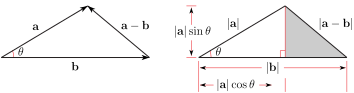
\includegraphics[width=\linewidth]{figs/cosineB}
\end{sbspanel}%
\end{sidebyside}%
\par
That triangle is a right triangle whose hypotenuse has length \(|\va-\vb|\) and  whose other two sides have lengths \(\big(|\vb|-|\va|\cos\theta\big)\) and \(|\va|\sin\theta\). So Pythagoras gives%
\begin{align*}
|\va-\vb|^2&=\big(|\vb|-|\va|\cos\theta\big)^2+
\big(|\va|\sin\theta\big)^2\\
&=|\vb|^2-2|\va|\,|\vb|\,\cos\theta+|\va|^2\cos^2\theta
+|\va|^2\sin^2\theta\\
&=|\vb|^2-2|\va|\,|\vb|\,\cos\theta+|\va|^2
\end{align*}
This is precisely the cosine law\footnote{You may be used to seeing it written as \(c^2=a^2+b^2-2 a b \cos C\), where \(a\), \(b\) and \(c\) are the lengths of the three sides of the triangle and \(C\) is the angle opposite the side of length \(c\)\label{g:fn:idm45408034558800}}. Observe that, when \(\theta=\tfrac{\pi}{2}\), this reduces to, (surprise!) Pythagoras' theorem.%
\par
Setting our two expressions for \(|\va-\vb|^2\) equal to each other,%
\begin{gather*}
|\va-\vb|^2=|\va|^2+|\vb|^2-2\va\cdot\vb
=|\vb|^2-2|\va|\,|\vb|\,\cos\theta+|\va|^2
\end{gather*}
cancelling the \(|\va|^2\) and \(|\vb|^2\) common to both sides%
\begin{gather*}
-2\va\cdot\vb
=-2|\va|\,|\vb|\,\cos\theta
\end{gather*}
and dividing by \(-2\) gives%
\begin{gather*}
\va\cdot\vb=|\va|\,|\vb|\,\cos\theta
\end{gather*}
which is exactly property 6.%
\par
Property 7 follows directly from property 6. First note that the dot product \(\va\cdot\vb=|\va|\,|\vb|\,\cos\theta\) is zero if and only if at least one of the three factors \(|\va|,\ |\vb|,\ \cos\theta\) is zero. The first factor is zero if and only if \(\va=\vZero \). The second factor is zero if and only if \(\vb=\vZero \). The third factor is zero if and only if \(\theta=\pm\tfrac{\pi}{2}+2k\pi\), for some integer \(k\), which in turn is true if and only if \(\va\) and \(\vb\) are mutually perpendicular.%
\end{proof}
Because of Property 7 of Theorem \hyperref[x:theorem:thm_dotPppties]{{\xreffont\ref{x:theorem:thm_dotPppties}}}, the dot product can be used to test whether or not two vectors are perpendicular to each other. That is, whether or not the angle between the two vectors is \(90^\circ\). Another name\footnote{The concepts of the dot product and perpendicularity have been generalized a lot in mathematics (for example, from 2d and 3d vectors to functions). The generalization of the dot product is called the ``inner product'' and the generalization of perpendicularity is called ``orthogonality''.\label{g:fn:idm45408034710576}} for ``perpendicular'' is ``orthogonal''. Testing for orthogonality is one of the main uses of the dot product.%
\begin{example}{}{g:example:idm45408034745552}%
Consider the three vectors%
\begin{equation*}
\va=\llt 1,1,0 \rgt\qquad
\vb=\llt 1,0,1 \rgt \qquad
\vc=\llt -1,1,1\rgt
\end{equation*}
Their dot products%
\begin{alignat*}{3}
\va\cdot\vb & = \llt 1,1,0 \rgt \cdot \llt 1,0,1 \rgt
&& = 1\times 1 +1\times 0+0\times 1
&& = 1\\
\va\cdot\vc & = \llt 1,1,0 \rgt \cdot \llt -1,1,1 \rgt
&& = 1\times(-1) +1\times 1+0\times 1
&& = 0\\
\vb\cdot\vc & = \llt 1,0,1 \rgt \cdot \llt -1,1,1 \rgt
&& = 1\times(-1) +0\times 1+1\times 1
&& = 0
\end{alignat*}
tell us that \(\vc\) is perpendicular to both \(\va\) and \(\vb\). Since both \(|\va|=|\vb|=\sqrt{1^2+1^2+0^2}=\sqrt{2}\) the first dot product tells us that the angle, \(\theta\), between \(\va\) and \(\vb\) obeys%
\begin{gather*}
\cos\theta =\frac{\va\cdot\vb}{|\va|\,|\vb|}=\frac{1}{2}
\implies
\theta =\frac{\pi}{3}
\end{gather*}
%
\begin{sidebyside}{1}{0.3}{0.3}{0}%
\begin{sbspanel}{0.4}%
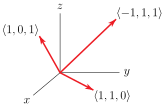
\includegraphics[width=\linewidth]{figs/dotProd}
\end{sbspanel}%
\end{sidebyside}%
\end{example}
Dot products are also used to compute projections.  First, here's the definition.%
\begin{definition}{Projection.}{x:definition:def_projection}%
Draw two vectors, \(\va\) and \(\vb\), with their tails at a common point and drop a perpendicular from the head of \(\va\) to the line that passes through both the head and tail of \(\vb\). By definition, the projection of the vector \(\va\) on the vector \(\vb\) is the vector from the tail of \(\vb\) to the point on the line where the perpendicular hits.%
\begin{sidebyside}{2}{0.11}{0.11}{0.22}%
\begin{sbspanel}{0.23}[center]%
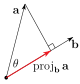
\includegraphics[width=\linewidth]{figs/projA}
\end{sbspanel}%
\begin{sbspanel}{0.33}[center]%
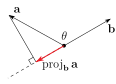
\includegraphics[width=\linewidth]{figs/projB}
\end{sbspanel}%
\end{sidebyside}%
\end{definition}
Think of the projection of \(\va\) on \(\vb\) as the part of \(\va\) that is in the direction of \(\vb\).%
\par
Now let's develop a formula for the projection of \(\va\) on \(\vb\). Denote by \(\theta\) the angle between \(\va\) and \(\vb\). If \(|\theta|\) is no more than \(90^\circ\), as in the figure on the left above, the length of the projection of \(\va\) on \(\vb\) is \(|\va|\cos\theta\). By Property 6 of Theorem \hyperref[x:theorem:thm_dotPppties]{{\xreffont\ref{x:theorem:thm_dotPppties}}}, \(|\va|\cos\theta=\va\cdot\vb/|\vb|\), so the projection is a vector whose length is \(\va\cdot\vb/|\vb|\) and whose direction is given by the unit vector \(\vb/|\vb|\). Hence%
\begin{gather*}
\text{projection of \(\va\) on \(\vb\)}={\rm proj}_{\vb}\,\va
=\frac{\va\cdot\vb}{|\vb|}\frac{\vb}{|\vb|}
=\frac{\va\cdot\vb}{|\vb|^2}\,\vb
\end{gather*}
If \(|\theta|\) is larger than \(90^\circ\), as in the figure on the right above, the projection has length \(|\va|\,\cos(\pi-\theta)=-|\va|\cos\theta=-\va\cdot\vb/|\vb|\) and direction \(-\vb/|\vb|\). In this case%
\begin{gather*}
{\rm proj}_{\vb}\,\va
=-\frac{\va\cdot\vb}{|\vb|}\ \frac{-\vb}{|\vb|}
=\frac{\va\cdot\vb}{|\vb|^2}\ \vb
\end{gather*}
too. So the formula%
\begin{fact}{}{}{x:fact:eqn_proj}%
%
\begin{equation*}
{\rm proj}_{\vb}\,\va=\frac{\va\cdot\vb}{|\vb|^2}\,\vb
\end{equation*}
%
\end{fact}
is applicable whenever \(\vb\ne\vZero \). We may rewrite \({\rm proj}_{\vb}\,\va=\frac{\va\cdot\vb}{|\vb|}\,\frac{\vb}{|\vb|}\). The coefficient, \(\frac{\va\cdot\vb}{|\vb|}\), of the unit vector \(\frac{\vb}{|\vb|}\), is called the component of \(\va\) in the direction \(\vb\). As a special case, if \(\vb\) happens to be a unit vector, which, for emphasis, we'll now write has \(\hat\vb\), the projection formula simplifies to%
\begin{fact}{}{}{x:fact:eqn_unit_proj}%
%
\begin{equation*}
{\rm proj}_{\hat\vb}\,\va
=  (\va\cdot\hat\vb)\,\hat\vb
\end{equation*}
%
\end{fact}
\begin{example}{}{x:example:eg_proj}%
In this example, we will find the projection of the vector \(\llt 0,3\rgt\) on the vector \(\llt 1,1\rgt\), as in the figure%
\begin{sidebyside}{1}{0.3}{0.3}{0}%
\begin{sbspanel}{0.4}%
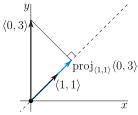
\includegraphics[width=\linewidth]{figs/projEg}
\end{sbspanel}%
\end{sidebyside}%
\par
By Equation \hyperref[x:fact:eqn_proj]{{\xreffont\ref{x:fact:eqn_proj}}} with \(\va=\llt 0,3\rgt\) and \(\vb=\llt 1,1\rgt\), that projection is%
\begin{align*}
{\rm proj}_{\llt 1,1\rgt}\,\llt 0,3\rgt
&=\frac{\llt 0,3\rgt\cdot\llt 1,1\rgt}{|\llt 1,1\rgt|^2}\,\llt 1,1\rgt\\
&=\frac{0\times1+3\times 1}{1^2+1^2}\,\llt 1,1\rgt
=\llt \frac{3}{2},\frac{3}{2}\rgt
\end{align*}
%
\end{example}
One use of projections is to ``resolve forces''. There is an example in the next (optional) section.%
\end{subsectionptx}
%
%
\typeout{************************************************}
\typeout{Subsection 1.2.3 (Optional) Using Dot Products to Resolve Forces \textemdash{} The Pendulum}
\typeout{************************************************}
%
\begin{subsectionptx}{(Optional) Using Dot Products to Resolve Forces \textemdash{} The Pendulum}{}{(Optional) Using Dot Products to Resolve Forces \textemdash{} The Pendulum}{}{}{x:subsection:subsec-pendulum}
Model a pendulum by a mass \(m\) that is connected to a hinge by an idealized rod that is massless and of fixed length \(\ell\). Denote by \(\theta\) the angle between the rod and vertical. The forces acting on the mass are%
\begin{itemize}[label=\textbullet]
\item{}gravity, which has magnitude \(mg\) and direction \(\llt 0,-1\rgt\),%
\item{}tension in the rod, whose magnitude \(\tau(t)\) automatically adjusts itself so that the distance between the mass and the hinge is fixed at \(\ell\) (so that the rod does not stretch or contract) and whose direction is always parallel to the rod,%
\item{}and possibly some frictional forces, like friction in the hinge and air resistance. Assume that the total frictional force has magnitude proportional\footnote{The behaviour of air resistance (sometimes called drag) is pretty complicated. We're using a reasonable low speed approximation. At high speeds drag is typically proportional to the square of the speed.\label{g:fn:idm45408035248560}} to the speed of the mass and has direction opposite to the direction of motion of the mass. We'll call the constant of proportionality \(\beta\).%
\end{itemize}
%
\begin{sidebyside}{1}{0.275}{0.275}{0}%
\begin{sbspanel}{0.45}%
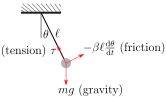
\includegraphics[width=\linewidth]{figs/pendulum3}
\end{sbspanel}%
\end{sidebyside}%
\par
If we use a coordinate system centered on the hinge, the \((x,y)\) coordinates of the mass at time \(t\) are%
\begin{align*}
x(t)&=\ell\sin\theta(t)\\
y(t)&=-\ell\cos\theta(t)
\end{align*}
where \(\theta(t)\) is the angle between the rod and vertical at time \(t\). We are now going to use Newton's law of motion%
\begin{gather*}
\text{mass}\times\text{acceleration}=\text{total applied force}
\end{gather*}
to determine now \(\theta\) evolves in time. By definition, the velocity and acceleration vectors\footnote{For a more comprehensive treatment of derivatives of vector valued functions \(\vr(t)\), and in particular of velocity and acceleration, see Section \hyperref[x:section:sec_curves]{{\xreffont\ref{x:section:sec_curves}}} in this text and Section 1.1 in the CLP-4 text.\label{g:fn:idm45408035314736}} for the position vector \(\llt x(t),y(t)\rgt\) are%
\begin{align*}
\diff{}{t}\llt x(t),y(t)\rgt
&= \llt \diff{x}{t}(t),\diff{y}{t}(t)\rgt\\
\ddiff{2}{}{t}\llt x(t),y(t)\rgt
&=\llt \ddiff{2}{x}{t}(t),\ddiff{2}{y}{t}(t)\rgt
\end{align*}
So, the velocity and acceleration vectors of our mass are%
\begin{alignat*}{1}
\vv(t)&=\diff{}{t}\llt x(t),y(t)\rgt\\
&=\llt \ell\diff{}{t}\sin\theta(t),-\ell\diff{}{t}\cos\theta(t)\rgt\\
&=\llt \ell\cos\theta(t)\,\diff{\theta}{t}(t)\,,\,
\ell\sin\theta(t)\,\diff{\theta}{t}(t)\rgt\\
&=\ell\,\diff{\theta}{t}(t)\,\llt \cos\theta(t),\sin\theta(t)\rgt\\
\va(t)&=\ddiff{2}{}{t}\llt x(t),y(t)\rgt\\
&=\diff{}{t}
\left\{\ell\,\diff{\theta}{t}(t)\,
\llt \cos\theta(t),\sin\theta(t)\rgt \right\}\\
&=\ell\,\ddiff{2}{\theta}{t}(t)\,\llt \cos\theta(t),\sin\theta(t)\rgt
+\ell\,\diff{\theta}{t}(t)
\llt \diff{}{t}\cos\theta(t),\diff{}{t}\sin\theta(t)\rgt\\
&= \ell\,\ddiff{2}{\theta}{t}(t)\llt \cos\theta(t),\sin\theta(t)\rgt
+\ell \Big(\diff{\theta}{t}(t)\Big)^2
\llt -\sin\theta(t),\cos\theta(t)\rgt
\end{alignat*}
%
\par
The negative of the velocity vector is \(- \ell\, \diff{\theta}{t}\llt \cos\theta,\sin\theta\rgt\), so the total frictional force is%
\begin{equation*}
-\beta\ell\, \diff{\theta}{t}\llt \cos\theta,\sin\theta\rgt
\end{equation*}
with \(\beta\) our constant of proportionality.%
\par
The vector%
\begin{equation*}
\tau(t) \llt -\sin\theta(t),\cos\theta(t)\rgt
\end{equation*}
has magnitude \(\tau(t)\) and direction parallel to the rod pointing from the mass towards the hinge and so is the force due to tension in the rod.%
\par
Hence, for this physical system, Newton's law of motion is%
\begin{align*}
&\overbrace{m\ell\,\ddiff{2}{\theta}{t}\llt \cos\theta,\sin\theta\rgt
+m\ell\,\Big(\diff{\theta}{t}\Big)^2\llt -\sin\theta,\cos\theta\rgt}^
{\text{mass}\times\text{acceleration}}\\
&\hskip1in=
\overbrace{mg\llt 0,-1\rgt}^{\rm gravity}
+\overbrace{\tau \llt -\sin\theta,\cos\theta\rgt}^{\rm tension}
-\overbrace{\beta\ell\,\diff{\theta}{t}\llt \cos\theta,\sin\theta\rgt}^{\rm friction}
\tag{\(*\)}
\end{align*}
This is a rather complicated looking equation. Writing out its \(x\)- and \(y\)-components doesn't help. They also look complicated. Instead, the equation can be considerably simplified (and consequently better understood) by ``taking its components parallel to and perpendicular to the direction of motion''. From the velocity vector \(\vv(t)\), we see that \(\llt \cos\theta(t),\sin\theta(t)\rgt \) is a unit vector parallel to the direction of motion at time \(t\). Recall, from \hyperref[x:fact:eqn_unit_proj]{{\xreffont\ref{x:fact:eqn_unit_proj}}}, that the projection of any vector \(\vb\) on any unit vector \(\hat\vd\) (with the ``hat'' on \(\hat\vd\) reminding ourselves that the vector is a unit vector) is%
\begin{gather*}
\big(\vb\cdot \hat\vd\big)\,\hat\vd
\end{gather*}
The coefficient \(\vb\cdot \hat\vd\) is, by definition, the component of \(\vb\) in the direction \(\hat\vd\). So, by dotting both sides of the equation of motion \((*)\) with \(\hat\vd=\llt \cos\theta(t),\sin\theta(t)\rgt \), we extract the component parallel to the direction of motion. Since%
\begin{align*}
\llt \cos\theta,\sin\theta\rgt \cdot\llt \cos\theta,\sin\theta\rgt &=1\\
\llt \cos\theta,\sin\theta\rgt \cdot\llt -\sin\theta,\cos\theta\rgt &=0\\
\llt \cos\theta,\sin\theta\rgt \cdot\llt 0,-1\rgt &=-\sin\theta
\end{align*}
this gives%
\begin{gather*}
m\ell\ddiff{2}{\theta}{t}=-mg\sin\theta-\beta\ell\diff{\theta}{t}
\end{gather*}
which is \emph{much} cleaner than \((*)\)! When \(\theta\) is small, we can approximate \(\sin\theta\approx\theta\) and get the equation%
\begin{gather*}
\ddiff{2}{\theta}{t}+\frac{\beta}{m}\diff{\theta}{t}+\frac{g}{\ell}\theta=0
\end{gather*}
which is easily solved. There are systematic procedures for finding the solution, but we'll just guess.%
\par
When there is no friction (so that \(\beta=0\)), we would expect the pendulum to just oscillate. So it is natural to guess%
\begin{equation*}
\theta(t)=A\sin(\omega t-\delta)
\end{equation*}
which is an oscillation with (unknown) amplitude \(A\), frequency \(\omega\) (radians per unit time) and phase \(\delta\). Substituting this guess into the left hand side, \(\theta''  + \tfrac{g}{\ell}\theta\),  yields%
\begin{equation*}
-A\omega^2\sin(\omega t-\delta)+A\tfrac{g}{\ell}\sin(\omega t-\delta)
\end{equation*}
which is zero if \(\omega=\sqrt{g/\ell}\). So \(\ \theta(t)=A\sin(\omega t-\delta)\ \) is a solution for any amplitude \(A\) and phase \(\delta\), provided the frequency \(\omega=\sqrt{g/\ell}\).%
\par
When there is some, but not too much, friction, so that \(\beta \gt 0\) is relatively small, we would expect ``oscillation with decaying amplitude''. So we  guess%
\begin{equation*}
\theta(t)=Ae^{-\gamma t}\sin(\omega t-\delta)
\end{equation*}
for some constant decay rate \(\gamma\), to be determined. With this guess,%
\begin{alignat*}{3}
\theta(t)&=\phantom{- -\gamma\omega^{2})} Ae^{-\gamma t}
&\sin(\omega t-\delta)\\
\theta'(t)&=\phantom{-\omega^{2})}-\gamma Ae^{-\gamma t}
&\sin(\omega t-\delta)
&+\phantom{2\gamma }\omega A e^{-\gamma t}&\cos(\omega t-\delta)\\
\theta''(t)&=(\gamma^2-\omega^2)Ae^{-\gamma t}&\sin(\omega t-\delta)
&-2\gamma\omega A e^{-\gamma t}&\cos(\omega t-\delta)
\end{alignat*}
and the left hand side%
\begin{align*}
\ddiff{2}{\theta}{t}+\frac{\beta}{m}\diff{\theta}{t}+\frac{g}{\ell}\theta
&
=\left[\gamma^2-\omega^2-\frac{\beta}{m}\gamma+\frac{g}{\ell}\right]
Ae^{-\gamma t}\sin(\omega t-\delta)\\
&\hskip0.5in+\left[-2\gamma\omega+\frac{\beta}{m}\omega\right]
Ae^{-\gamma t}\cos(\omega t-\delta)
\end{align*}
vanishes if \(\gamma^2-\omega^2-\frac{\beta}{m}\gamma+\tfrac{g}{\ell}=0\) and \(-2\gamma\omega+\frac{\beta}{m}\omega=0.\) The second equation tells us the decay rate \(\gamma=\tfrac{\beta}{2m}\) and then the first tells us the frequency%
\begin{gather*}
\omega=\sqrt{\gamma^2-\tfrac{\beta}{m}\gamma+\tfrac{g}{\ell}}
=\sqrt{\tfrac{g}{\ell}-\tfrac{\beta^2}{4m^2}}
\end{gather*}
When there is a lot of friction (namely when \(\tfrac{\beta^2}{4m^2} \gt \tfrac{g}{\ell}\), so that the frequency \(\omega\) is not a real number), we would expect damping without oscillation and so would guess \(\theta(t)=Ae^{-\gamma t}\). You can determine the allowed values of \(\gamma\) by substituting this guess in.%
\par
To extract the components perpendicular to the direction of motion, we dot with \(\llt -\sin\theta,\cos\theta\rgt \) rather than \(\llt \cos\theta,\sin\theta\rgt \). Note that, because%
\begin{equation*}
\llt -\sin\theta,\cos\theta\rgt \cdot \llt \cos\theta,\sin\theta\rgt =0,
\end{equation*}
the vector \(\llt -\sin\theta,\cos\theta\rgt \) really is perpendicular to the direction of motion.  Since%
\begin{align*}
\llt -\sin\theta,\cos\theta\rgt \cdot\llt \cos\theta,\sin\theta\rgt &=0\\
\llt -\sin\theta,\cos\theta\rgt \cdot\llt -\sin\theta,cos\theta\rgt &=1\\
\llt -\sin\theta,\cos\theta\rgt \cdot\llt 0,-1\rgt &=-\cos\theta
\end{align*}
dotting both sides of the equation of motion \((*)\) with \(\llt -\sin\theta,\cos\theta\rgt \) gives%
\begin{gather*}
m\ell\Big(\diff{\theta}{t}\Big)^2=-mg\cos\theta+\tau
\end{gather*}
This equation just determines the tension%
\begin{equation*}
\tau=m\ell\big(\diff{\theta}{t}\big)^2+mg\cos\theta
\end{equation*}
in the rod, once you know \(\theta(t)\).%
\end{subsectionptx}
%
%
\typeout{************************************************}
\typeout{Subsection 1.2.4 (Optional) Areas of Parallelograms}
\typeout{************************************************}
%
\begin{subsectionptx}{(Optional) Areas of Parallelograms}{}{(Optional) Areas of Parallelograms}{}{}{x:subsection:sec_GEOparallelogram}
A parallelogram is naturally determined by the two vectors that define its sides. We'll now develop a formula for the area of a parallelogram in terms of these two vectors.%
\par
Construct a parallelogram as follows. Pick two vectors \(\llt a,b\rgt \) and \(\llt c,d\rgt \). Draw them with their tails at a common point. Then draw \(\llt a,b\rgt \) a second time with its tail at the head of \(\llt c,d\rgt \) and draw  \(\llt c,d\rgt \) a second time with its tail at the head of \(\llt a,b\rgt \). If the common point is the origin, you get a picture like the figure below.%
\begin{sidebyside}{1}{0.17}{0.17}{0}%
\begin{sbspanel}{0.66}%
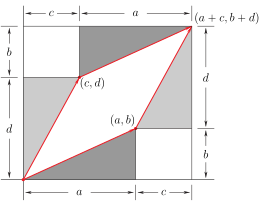
\includegraphics[width=\linewidth]{figs/area3}
\end{sbspanel}%
\end{sidebyside}%
\par
Any parallelogram can be constructed like this if you pick the common point and two vectors appropriately. Let's compute the area of the parallelogram. The area of the large rectangle with vertices \((0,0),\ (0, b+d),\ (a+c,0)\) and \((a+c,b+d)\) is \((a+c)(b+d)\). The parallelogram we want can be extracted from the large rectangle by deleting the two small rectangles (each of area \(bc\)), and the two lightly shaded triangles (each of area \(\half cd\)), and the two darkly shaded triangles (each of area \(\half ab\)). So the desired%
\begin{gather*}
{\rm area} = (a+c)(b+d) - (2\times bc) -\big(2\times \half cd\big)
-\big(2\times\half ab\big)
=ad-bc
\end{gather*}
In the above figure, we have implicitly assumed that \(a,\ b,\ c,\ d\ge 0\) and \(d/c\ge b/a\). In words, we have assumed that both vectors \(\llt a,b\rgt ,\ \llt c,d\rgt \) lie in the first quadrant and that \(\llt c,d\rgt \) lies above \(\llt a,b\rgt \). By simply interchanging \(a\leftrightarrow c\) and \(b\leftrightarrow d\) in the picture and throughout the argument, we see that when \(a,\ b,\ c,\ d\ge 0\) and \(b/a\ge d/c\), so that the vector \(\llt c,d\rgt \) lies below \(\llt a,b\rgt \), the area of the parallelogram is \(bc-ad\). In fact, all cases are covered by the formula%
\begin{fact}{}{}{x:fact:eq_pgram_area}%
%
\begin{gather*}
\text{area of parallelogram with sides }
\llt a,b\rgt
\text{ and }
\llt c,d\rgt =|ad-bc|
\end{gather*}
%
\end{fact}
Given two vectors \(\llt a,b\rgt \) and \(\llt c,d\rgt \), the expression \(ad-bc\) is generally written%
\begin{align*}
\det\left[\begin{matrix}a&b\\
c&d\end{matrix}\right]=ad-bc
\end{align*}
and is called the \emph{determinant} of the matrix\footnote{The topics of matrices and determinants appear prominently in linear algebra courses. We are only going to use them as notation, and we will explicitly explain that notation. A linear algebra course is \emph{not} a prerequisite for this text.\label{g:fn:idm45408035933856}}%
\begin{align*}
\left[\begin{matrix}a&b \\ c&d\end{matrix}\right]
\end{align*}
with rows \(\llt a,b\rgt \) and \(\llt c,d\rgt \). The determinant of a \(2\times 2\) matrix is the product of the diagonal entries minus the product of the off-diagonal entries.%
\par
There is a similar formula in three dimensions. Any three vectors \(\va=\llt a_1,a_2,a_3\rgt ,\ \vb=\llt b_1,b_2,b_3\rgt \) and \(\vc=\llt c_1,c_2,c_3\rgt \) in three dimensions%
\begin{sidebyside}{1}{0.4}{0.4}{0}%
\begin{sbspanel}{0.2}%
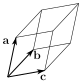
\includegraphics[width=\linewidth]{figs/piped}
\end{sbspanel}%
\end{sidebyside}%
\par
determine a parallelepiped (three dimensional parallelogram). Its volume is given by the formula%
\begin{fact}{}{}{x:fact:eq_piped_volume}%
%
\begin{align*}
\text{volume of parallelepiped with edges }
\va,\ \vb,\ \vc\
=\ \left|
\det\left[\begin{matrix}a_1&a_2&a_3 \\  b_1&b_2&b_3\\ c_1&c_2&c_3\end{matrix}\right]
\right|
\end{align*}
%
\end{fact}
The determinant of a \(3\times 3\) matrix can be defined in terms of some \(2\times 2\) determinants by%
\begin{sidebyside}{1}{0.025}{0.025}{0}%
\begin{sbspanel}{0.95}%
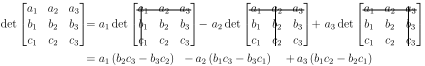
\includegraphics[width=\linewidth]{figs/det2}
\end{sbspanel}%
\end{sidebyside}%
\par
This formula is called ``expansion along the top row''. There is one term in the formula for each entry in the top row of the \(3\times 3\) matrix. The term is a sign times the entry itself times the determinant of the \(2\times 2\) matrix gotten by deleting the row and column that contains the entry. The sign alternates, starting with a ``\(+\)''.%
\par
We shall not prove this formula completely here\footnote{For a full derivation, see Example \hyperref[x:example:eg_GEOcross]{{\xreffont\ref{x:example:eg_GEOcross}}}\label{g:fn:idm45408036050032}}. It gets a little tedious. But, there is one case in which we can easily verify that the volume of the parallelepiped is really given by the absolute value of the claimed determinant. If the vectors \(\vb\) and \(\vc\) happen to lie in the \(xy\) plane, so that \(b_3=c_3=0\), then%
\begin{align*}
\det\left[\begin{matrix}
a_1&a_2&a_3\\ b_1&b_2&0\\ c_1&c_2&0
\end{matrix}\right]
&=a_1(b_20-0c_2) -a_2(b_10-0c_1) +a_3(b_1c_2-b_2c_1)\\
&=a_3(b_1c_2-b_2c_1)
\end{align*}
The first factor, \(a_3\), is the \(z\)-coordinate of the one vector not contained in the \(xy\)-plane. It is (up to a sign) the height of the parallelepiped. The second factor is, up to a sign, the area of the parallelogram determined by \(\vb\) and \(\vc\). This parallelogram forms the base of the parallelepiped. The product is indeed, up to a sign, the volume of the parallelepiped. That the formula is true in general is a consequence of the fact (that we will not prove) that the value of a determinant does not change when one rotates the coordinate system and that one can always rotate our coordinate axes around so that \(\vb\) and \(\vc\) both lie in the \(xy\)-plane.%
\end{subsectionptx}
%
%
\typeout{************************************************}
\typeout{Subsection 1.2.5 The Cross Product}
\typeout{************************************************}
%
\begin{subsectionptx}{The Cross Product}{}{The Cross Product}{}{}{x:subsection:subsec-crossprod}
We have already seen two different products involving vectors \textemdash{} the multiplication of a vector by a scalar and the dot product of two vectors. The dot product of two vectors yields a scalar. We now introduce another product of two vectors, called the \emph{cross product}. The cross product of two vectors will give a vector. There are applications which have two vectors as inputs and produce one vector as an output, and which are related to the cross product. Here is a very brief mention of two such applications. We will look at them in much more detail later.%
\begin{itemize}[label=\textbullet]
\item{}Consider a parallelogram in three dimensions. A parallelogram is naturally determined by the two vectors that define its sides. One measure of the size of a parallelogram is its area. One way to specify the orientation of the parallelogram is to give a vector that is perpendicular to it. A very compact way to encode both the area and the orientation of the parallelogram is to give a vector whose direction is perpendicular to the plane in which it lies and whose magnitude is its area. We shall see that such a vector can be easily constructed by taking the cross product (definition coming shortly) of the two vectors that give the sides of the parallelogram.%
\begin{sidebyside}{1}{0.325}{0.325}{0}%
\begin{sbspanel}{0.35}%
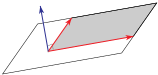
\includegraphics[width=\linewidth]{figs/pgramCross}
\end{sbspanel}%
\end{sidebyside}%
\item{}Imagine a rigid body which is rotating at a rate \(\Omega\) radians per second about an axis whose direction is given by the unit vector \(\hat\va\). Let \(P\) be any point on the body. We shall see, in the (optional) §\hyperref[x:subsection:sec_rot_motion]{{\xreffont\ref{x:subsection:sec_rot_motion}}}, that the velocity, \(\vv\), of the point \(P\) is the cross product (again, definition coming shortly) of the vector \(\Om\hat\va\) with the vector \(\vr\) from any point on the axis of rotation to \(P\).%
\begin{sidebyside}{1}{0.335}{0.335}{0}%
\begin{sbspanel}{0.33}%
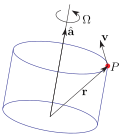
\includegraphics[width=\linewidth]{figs/rigidBB}
\end{sbspanel}%
\end{sidebyside}%
\end{itemize}
%
\par
Finally, here is the definition of the cross product. Note that it applies only to vectors in three dimensions.%
\begin{definition}{Cross Product.}{x:definition:def_crossProd}%
The cross product of the vectors \(\va=\llt a_1,a_2,a_3\rgt\) and \(\vb=\llt b_1,b_2,b_3\rgt\) is denoted \(\va\times\vb\) and is defined by%
\begin{gather*}
\va\times\vb = \llt a_2b_3-a_3b_2\,,\, a_3b_1-a_1b_3\,,\, a_1b_2-a_2b_1\rgt
\end{gather*}
%
\end{definition}
Note that each component has the form \(a_ib_j-a_jb_i\). The index \(i\) of the first \(a\) in component number \(k\) of \(\va\times\vb\) is just after \(k\) in the list \(1,2,3,1,2,3,1,2,3,\cdots\). The index \(j\) of the first \(b\) is just before \(k\) in the list.%
\begin{gather*}
(\va\times\vb)_k
=a_{{\rm just\  after\  }k}\ b_{{\rm just\  before\  }k}
-a_{{\rm just\  before\  }k}\ b_{{\rm just\  after\  }k}
\end{gather*}
For example, for component number \(k=3\),%
\begin{gather*}
\left.{\text{''just after 3'' is 1}}\atop{\text{''just before 3'' is 2}}\right\}
\implies (\va\times\vb)_3= a_1b_2-a_2b_1
\end{gather*}
%
\par
There is a much better way to remember this definition. Recall that a \(2\times 2\) matrix is an array of numbers having two rows and two columns and that the determinant of a \(2\times 2\) matrix is  defined by%
\begin{align*}
\det \left[\begin{matrix}a& b \\ c&d\end{matrix}\right]=ad-bc
\end{align*}
It is the product of the entries on the diagonal minus the product of the entries not on the diagonal.%
\par
A \(3\times 3\) matrix is an array of numbers having three rows and three columns.%
\begin{align*}
\left[\begin{matrix}
i& j &k
\\
a_1&a_2&a_3
\\
b_1&b_2&b_3\end{matrix}\right]
\end{align*}
You will shortly see why the entries in the top row have been given the rather peculiar names \(i\), \(j\) and \(k\). The determinant of a \(3\times 3\) matrix can be defined in terms of some \(2\times 2\) determinants by%
\begin{sidebyside}{1}{0.025}{0.025}{0}%
\begin{sbspanel}{0.95}%
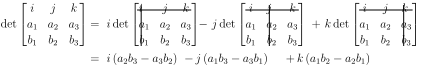
\includegraphics[width=\linewidth]{figs/det}
\end{sbspanel}%
\end{sidebyside}%
\par
This formula is called ``expansion of the determinant along the top row''. There is one term in the formula for each entry in the top row. The term is a sign times the entry itself times the determinant of the \(2\times 2\) matrix gotten by deleting the row and column that contains the entry. The sign alternates, starting with a \(+\). If we now replace \(i\) by \(\hi\), \(j\) by \(\hj\) and \(k\) by \(\hk\), we get exactly the formula for \(\va\times \vb\) of Definition \hyperref[x:definition:def_crossProd]{{\xreffont\ref{x:definition:def_crossProd}}}. That is the reason for the peculiar choice of names for the matrix entries. So%
\begin{align*}
\va\times\vb
&=\det\left[\begin{matrix}\hi& \hj &\hk
\\
a_1&a_2&a_3
\\
b_1&b_2&b_3\end{matrix}\right]\\
&=\hi\big(a_2b_3-a_3b_2) -\hj(a_1b_3-a_3b_1) +\hk(a_1b_2-a_2b_1)
\end{align*}
is a mnemonic device for remembering the definition of \(\va\times\vb\). It is also good from the point of view of evaluating \(\va\times\vb\). Here are several examples in which we use the determinant mnemonic device to evaluate cross products.%
\begin{example}{}{x:example:eg_GEOcrossijji}%
In this example, we'll use the mnemonic device to compute two very simple cross products. First%
\begin{sidebyside}{1}{0.025}{0.025}{0}%
\begin{sbspanel}{0.95}%
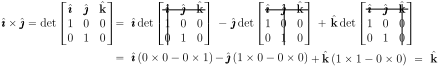
\includegraphics[width=\linewidth]{figs/detij}
\end{sbspanel}%
\end{sidebyside}%
\par
Second%
\begin{sidebyside}{1}{0.025}{0.025}{0}%
\begin{sbspanel}{0.95}%
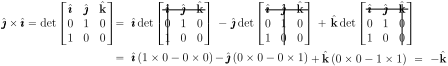
\includegraphics[width=\linewidth]{figs/detji}
\end{sbspanel}%
\end{sidebyside}%
\par
Note that, unlike most (or maybe even all) products that you have seen before, \(\hi\times\hj\) is \emph{not} the same as \(\hj\times\hi\)!%
\end{example}
\begin{example}{}{x:example:eg_GEOcrossEgA}%
In this example, we'll use the mnemonic device to compute two more complicated cross products. Let \(\va=\llt 1,2,3 \rgt\) and \(\vb=\llt 1,-1,2 \rgt\). First%
\begin{sidebyside}{1}{0.025}{0.025}{0}%
\begin{sbspanel}{0.95}%
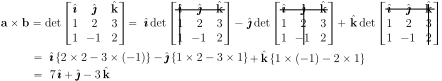
\includegraphics[width=\linewidth]{figs/detEgA1}
\end{sbspanel}%
\end{sidebyside}%
\par
Second%
\begin{sidebyside}{1}{0.025}{0.025}{0}%
\begin{sbspanel}{0.95}%
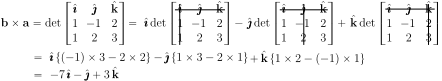
\includegraphics[width=\linewidth]{figs/detEgA2}
\end{sbspanel}%
\end{sidebyside}%
\par
Here are some important observations.%
\begin{itemize}[label=\textbullet]
\item{}The vectors \(\va\times\vb\) and \(\vb\times\va\) are not the same! In fact \(\vb\times\va=-\va\times\vb\). We shall see in Theorem \hyperref[x:theorem:thm_crossPppties]{{\xreffont\ref{x:theorem:thm_crossPppties}}} below that this was not a fluke.%
\item{}The vector \(\va\times\vb\) has dot product zero with both \(\va\) and \(\vb\). So the vector  \(\va\times\vb\) is prependicular to both \(\va\) and \(\vb\). We shall see in Theorem \hyperref[x:theorem:thm_crossPppties]{{\xreffont\ref{x:theorem:thm_crossPppties}}} below that this was also not a fluke.%
\end{itemize}
%
\end{example}
\begin{example}{}{x:example:eg_GEOcrossEgB}%
Yet again we use the mnemonic device to compute a more complicated cross product. This time let \(\va=\llt 3,2,1 \rgt\) and \(\vb=\llt 6,4,2 \rgt\). Then%
\begin{sidebyside}{1}{0.025}{0.025}{0}%
\begin{sbspanel}{0.95}%
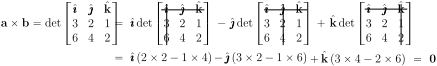
\includegraphics[width=\linewidth]{figs/detEgB}
\end{sbspanel}%
\end{sidebyside}%
\par
We shall see in Theorem \hyperref[x:theorem:thm_crossPppties]{{\xreffont\ref{x:theorem:thm_crossPppties}}} below that it is not a fluke that the cross product is \(\vZero\). It is a consequence of the fact that \(\va\) and \(\vb=2\va\) are parallel.%
\end{example}
We now move on to learning about the properties of the cross product. Our first properties lead up to a more intuitive geometric definition of \(\va\times\vb\), which is better for interpreting \(\va\times\vb\). These properties of the cross product, which state that  \(\va\times\vb\) is a vector and then determine its direction and length, are as follows. We will collect these properties, and a few others, into a theorem shortly. %
\begin{description}
\item[{(0)}]\(\va,\vb\)  are vectors in three dimensions and \(\va\times\vb\) is a vector in three dimensions.%
\item[{(1)}]\(\va\times\vb\) is perpendicular to both  \(\va\) and \(\vb\).%
\end{description}
%
\begin{proof}{}{g:proof:idm45408044294528}
To check that \(\va\) and \(\va\times \vb\) are perpendicular, one just has to check that the dot product \(\va\cdot(\va\times \vb)=0\). The six terms in%
\begin{equation*}
\va\cdot(\va\times \vb)=
a_1(a_2b_3-a_3b_2)+a_2(a_3b_1-a_1b_3)+a_3(a_1b_2-a_2b_1)
\end{equation*}
cancel pairwise. The computation showing that \(\vb\cdot(\va\times \vb)=0\) is similar.%
\end{proof}
%
\begin{description}
\item[{(2)}]%
\begin{align*}
|\va\times\vb| \amp = |\va|\,|\vb|\sin\theta
\text{ where } 0\le\theta\le\pi \text{ is the angle between } \va,\vb\\
\amp = \text{the area of the parallelogram with sides } \va, \vb
\end{align*}
%
\begin{sidebyside}{1}{0.4}{0.4}{0}%
\begin{sbspanel}{0.2}%
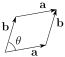
\includegraphics[width=\linewidth]{figs/area}
\end{sbspanel}%
\end{sidebyside}%
\end{description}
%
\begin{proof}{}{g:proof:idm45408044372496}
The formula \(|\va\times\vb|=|\va|\,|\vb|\sin\theta\) is gotten by verifying that%
\begin{align*}
|\va\times\vb|^2
&=\big(\va\times\vb\big)\cdot\big(\va\times\vb\big)\\
&=(a_2b_3-a_3b_2)^2+(a_3b_1-a_1b_3)^2+ (a_1b_2-a_2b_1)^2\\
&=a_2^2b_3^2-2a_2b_3a_3b_2+a_3^2b_2^2
+a_3^2b_1^2-2a_3b_1a_1b_3+a_1^2b_3^2\\
&\hskip0.5in
+a_1^2b_2^2-2a_1b_2a_2b_1+a_2^2b_1^2\\
\intertext{is equal to}
|\va|^2\,|\vb|^2\sin^2\theta
&=|\va|^2|\vb|^2(1-\cos^2\theta)\\
&=|\va|^2|\vb|^2-(\va\cdot\vb)^2\\
&=\big(a_1^2+a_2^2+a_3^2\big)\big(b_1^2+b_2^2+b_3^2\big)
-\big(a_1b_1+a_2b_2+a_3b_3\big)^2\\
&=a_1^2b_2^2+a_1^2b_3^2+a_2^2b_1^2+a_2^2b_3^2+a_3^2b_1^2+a_3^2b_2^2\\
&\hskip0.5in
-\big(2a_1b_1a_2b_2+2a_1b_1a_3b_3+2a_2b_2a_3b_3\big)
\end{align*}
To see that \(|\va|\,|\vb|\sin\theta\) is the area of the parallelogram with sides \(\va\) and \(\vb\), just recall that the area of any parallelogram is given by the length of its base times its height. Think of \(\va\) as the base of the parallelogram. Then \(|\va|\) is the length of the base and \(|\vb|\sin\theta\) is the height.%
\begin{sidebyside}{1}{0.39}{0.39}{0}%
\begin{sbspanel}{0.22}%
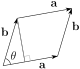
\includegraphics[width=\linewidth]{figs/areaB}
\end{sbspanel}%
\end{sidebyside}%
\end{proof}
These properties almost determine \(\va\times\vb\). Property 1 forces the vector \(\va\times\vb\) to lie on the line perpendicular to the plane containing \(\va\) and \(\vb\). There are precisely two vectors on this line that have the length given by property 2. In the left hand figure of%
\begin{sidebyside}{3}{0.055}{0.055}{0.11}%
\begin{sbspanel}{0.25}[center]%
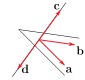
\includegraphics[width=\linewidth]{figs/crossLL}
\end{sbspanel}%
\begin{sbspanel}{0.22}[center]%
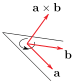
\includegraphics[width=\linewidth]{figs/crossRR}
\end{sbspanel}%
\begin{sbspanel}{0.2}[center]%
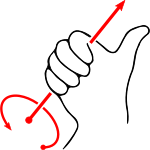
\includegraphics[width=\linewidth]{figs/RHR}
\end{sbspanel}%
\end{sidebyside}%
\par
the two vectors are labeled \(\vc\) and \(\vd\). Which of these two candidates is correct is determined by the right hand rule\footnote{That the cross product uses the right hand rule, rather than the left hand rule, is an example of the tyranny of the masses \textemdash{} only roughly 10\textbackslash{}\% of humans are left-handed.\label{g:fn:idm45408044497504}}, which says that if you form your right hand into a fist with your fingers curling from \(\va\) to \(\vb\), then when you stick your thumb straight out from the fist, it points in the direction of \(\va\times\vb\). This is illustrated in the figure on the right above\footnote{This figure is a variant of \url{https://commons.wikimedia.org/wiki/File:Right_hand_rule_simple.png}\label{g:fn:idm45408044522080}}. The important special cases%
\begin{description}
\item[{(3)}]%
\begin{equation*}
\hi\times\hj=\phantom{-}\hk,\ \ \ \hj\times\hk=\phantom{-}\hi,\ \ \  \hk\times\hi=\phantom{-}\hj
\end{equation*}
%
\begin{equation*}
\hj\times\hi=-\hk,\ \ \ \hk\times\hj=-\hi,\ \ \ \hi\times\hk=-\hj
\end{equation*}
all follow directly from the definition of the cross product (see, for example, Example \hyperref[x:example:eg_GEOcrossijji]{{\xreffont\ref{x:example:eg_GEOcrossijji}}}) and all obey the right hand rule.  Combining properties 1, 2 and the right hand rule give the geometric definition of \(\va\times\vb\). To remember these three special cases, just remember this figure.%
\begin{sidebyside}{1}{0.375}{0.375}{0}%
\begin{sbspanel}{0.25}%
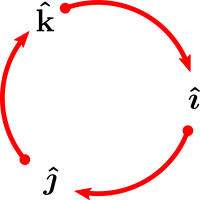
\includegraphics[width=\linewidth]{figs/cp_circle}
\end{sbspanel}%
\end{sidebyside}%
\par
The product of any two standard basis vectors, taken in the order of the arrows in the figure, is the third standard basis vector. Going against the arrows introduces a minus sign.%
\item[{(4)}]%
\begin{equation*}
\va\times\vb=|\va|\,|\vb|\sin\theta\ \hn
\end{equation*}
where \(\theta\) is the angle between \(\va, \vb\), \(|\hn|=1,\ \hn\perp\va,\vb\), and \((\va,\vb,\hn)\) obey the right hand rule.%
\end{description}
%
\begin{proof}{Outline of Proof.}{g:proof:idm45408044611456}
We have already seen that the right hand side has the correct length and, except possibly for a sign, direction. To check that the right hand rule holds in general, rotate your coordinate system around\footnote{Note that as you translate or rotate the coordinate system, the right hand rule is preserved. If \((\va,\vb,\hn)\) obey the right hand rule so do their rotated and translated versions.\label{g:fn:idm45408044615456}} so that \(\va\) points along the positive \(x\) axis and \(\vb\) lies in the \(xy\)-plane with positive \(y\) component. That is \(\va=\alpha\hi\) and \(\vb=\beta\hi+\gamma\hj\) with \(\alpha,\gamma\ge 0\). Then%
\begin{equation*}
\va\times\vb=\alpha\hi\times(\beta\hi+\gamma\hj) =\alpha\beta\,\hi\times\hi+\alpha\gamma\,\hi\times\hj.
\end{equation*}
The first term vanishes by property 2, because the angle \(\theta\) between \(\hi\) and \(\hi\) is zero. So, by property 3, \(\va\times\vb= \alpha\gamma\hk\) points along the positive \(z\) axis, which is consistent with the right hand rule.%
\end{proof}
The analog of property 7 of the dot product (which says that \(\va\cdot\vb\) is zero if and only if  \(\va=\vZero\) or \(\vb=\vZero\) or  \(\va\perp\vb\)) follows immediately from property 2.%
\begin{description}
\item[{(5)}]%
\begin{equation*}
\va\times\vb=\vZero\iff \va=\vZero  \text{ or }
\vb=\vZero
\text{ or }
\va\parallel\vb.
\end{equation*}
%
\end{description}
%
\par
The remaining properties are all tools for helping do computations with cross products. Here is a theorem which summarizes the properties of the cross product. We have already seen the first five. The other properties are all tools for helping do computations with cross products.%
\begin{theorem}{Properties of the Cross Product.}{}{x:theorem:thm_crossPppties}%
%
\begin{description}
\item[{(0)}]\(\va,\vb\)  are vectors in three dimensions and \(\va\times\vb\) is a vector in three dimensions.%
\item[{(1)}]\(\va\times\vb\) is perpendicular to both  \(\va\) and \(\vb\).%
\item[{(2)}]%
\begin{align*}
|\va\times\vb| \amp = |\va|\,|\vb|\sin\theta
\text{ where } 0\le\theta\le\pi \text{ is the angle between } \va,\vb\\
\amp = \text{the area of the parallelogram with sides } \va, \vb
\end{align*}
%
\begin{sidebyside}{1}{0.375}{0.375}{0}%
\begin{sbspanel}{0.25}%
\includegraphics[width=\linewidth]{figs/area}
\end{sbspanel}%
\end{sidebyside}%
\item[{(3)}]%
\begin{equation*}
\hi\times\hj=\phantom{-}\hk,\ \ \ \hj\times\hk=\phantom{-}\hi,\ \ \  \hk\times\hi=\phantom{-}\hj
\end{equation*}
%
\item[{(4)}]%
\begin{equation*}
\va\times\vb=|\va|\,|\vb|\sin\theta\ \hn
\end{equation*}
where \(\theta\) is the angle between \(\va, \vb\), \(|\hn|=1,\ \hn\perp\va,\vb\), and \((\va,\vb,\hn)\) obey the right hand rule.%
\item[{(5)}]%
\begin{equation*}
\va\times\vb=\vZero\iff \va=\vZero  \text{ or }
\vb=\vZero
\text{ or }
\va\parallel\vb.
\end{equation*}
%
\item[{(6)}]%
\begin{equation*}
\va\times \vb=-\vb\times\va
\end{equation*}
%
\item[{(7)}]%
\begin{equation*}
(s\va)\times \vb=\va\times(s\vb)=s(\va\times \vb)
\end{equation*}
for any scalar (i.e. number) \(s\).%
\item[{(8)}]%
\begin{equation*}
\va\times(\vb+\vc)=\va\times\vb+\va\times \vc
\end{equation*}
%
\item[{(9)}]%
\begin{equation*}
\va\cdot(\vb\times\vc)=(\va\times\vb)\cdot\vc
\end{equation*}
%
\item[{(10)}]%
\begin{equation*}
\va\times(\vb\times\vc)=(\vc\cdot\va)\vb -(\vb\cdot\va)\vc
\end{equation*}
%
\end{description}
%
\end{theorem}
\begin{proof}{}{g:proof:idm45408044919104}
We have already seen the proofs up to number 5. Numbers 6, 7 and 8 follow immediately from the definition, using a little algebra. To prove numbers 9 and 10 we just write out the definitions of the left hand sides and the right hand sides and observe that they are equal.%
\par
%
\begin{description}
\item[{(9)}]The left hand side is%
\begin{align*}
\va\cdot(\vb\times\vc)
&=\llt a_1,a_2,a_3\rgt\cdot
\llt b_2c_3\!-\!b_3c_2\,,\, b_3c_1\!-\!b_1c_3\,,\, b_1c_2\!-\!b_2c_1\rgt\\
&={\color{blue}{a_1b_2c_3}} \!-\! {\color{blue}{a_1b_3c_2}} \!+\! {\color{orange}{a_2b_3c_1}} \!-\! {\color{orange}{a_2b_1c_3}} \!+\! a_3b_1c_2 \!-\! a_3b_2c_1
\end{align*}
The right hand side is%
\begin{align*}
(\va\times\vb)\cdot\vc
&=\llt a_2b_3\!-\!a_3b_2\,,\, a_3b_1\!-\!a_1b_3\,,\, a_1b_2\!-\!a_2b_1\rgt\cdot
\llt c_1,c_2,c_3\rgt\\
&={\color{orange}{a_2b_3c_1}} \!-\! a_3b_2c_1 \!+\! a_3b_1c_2 \!-\! {\color{blue}{a_1b_3c_2}} \!+\! {\color{blue}{a_1b_2c_3}} \!-\! {\color{orange}{a_2b_1c_3}}
\end{align*}
The left and right hand sides are the same.%
\item[{(10)}]We will give the straightforward, but slightly tedious, computations in (the optional) §\hyperref[x:subsection:sec_vector_identities]{{\xreffont\ref{x:subsection:sec_vector_identities}}}.%
\end{description}
%
\end{proof}
\begin{warning}{}{x:warning:warning_GEOMcross}%
Take particular care with properties 6 and 10. They are counterintuitive and are a frequent source of errors. In particular, for general vectors \(\va\), \(\vb\), \(\vc\), the cross product is neither commutative nor associative, meaning that%
\begin{align*}
\va\times\vb&\ne\vb\times\va\\
\va\times(\vb\times\vc)&\ne (\va\times\vb)\times\vc
\end{align*}
For example%
\begin{align*}
\hi\times(\hi\times\hj)
&=\hi\times\hk=-\hk\times\hi =-\hj\\
(\hi\times \hi)\times\hj&= \vZero \times\hj=\vZero
\end{align*}
%
\end{warning}
\begin{example}{}{x:example:eg_GEOcross}%
As an illustration of the properties of the dot and cross product, we now derive the formula for the volume of the parallelepiped with edges \(\va=\llt a_1,a_2,a_3\rgt \), \(\vb = \llt b_1,b_2,b_3\rgt \), \(\vc = \llt c_1,c_2,c_3\rgt \) that was mentioned in §\hyperref[x:subsection:sec_GEOparallelogram]{{\xreffont\ref{x:subsection:sec_GEOparallelogram}}}.%
\begin{sidebyside}{1}{0.25}{0.25}{0}%
\begin{sbspanel}{0.5}%
\includegraphics[width=\linewidth]{figs/pipedVolume}
\end{sbspanel}%
\end{sidebyside}%
\par
The volume of the parallelepiped is the area of its base times its height\footnotemark{}. The base is the parallelogram with sides \(\vb\) and \(\vc\). Its area is the length of its base, which is \(|\vb|\), times its height, which is \(|\vc|\,\sin\theta\). (Drop a perpendicular from the head of \(\vc\) to the line containing \(\vb\)). Here \(\theta\) is the angle between \(\vb\) and \(\vc\). So the area of the base is \(|\vb|\,|\vc|\,\sin\theta= |\vb\times\vc|\), by property 2 of the cross product.%
\par
To get the height of the parallelepiped, we drop a perpendicular from the head of \(\va\) to the line that passes through the tail of \(\va\) and is perpendicular to the base of the parallelepiped. In other words, from the head of \(\va\) to the line that contains both the head and the tail of \(\vb\times\vc\). So the height of the parallelepiped is \(|\va|\,|\cos\varphi|\).  (The absolute values have been included because if the angle between \(\vb\times\vc\) and \(\va\) happens to be greater than \(90^\circ\), the \(\cos\varphi\) produced by taking the dot product of \(\va\) and  \((\vb\times\vc\)) will be negative.)%
\par
All together%
\begin{align*}
\text{volume of parallelepiped}
&=(\text{area of base})\,(\text{height})\\
&=|\vb\times\vc|\ |\va|\ |\cos\varphi|\\
&=\big|\va\cdot(\vb\times\vc)\big|\\
&=\left|a_1 (\vb\times\vc)_1 +a_2 (\vb\times\vc)_2
+a_3 (\vb\times\vc)_3\right|\\
&=\left|a_1\det\left[\begin{matrix} b_2&b_3 \\ c_2&c_3\end{matrix}\right]
-a_2 \det\left[\begin{matrix}b_1&b_3 \\ c_1&c_3\end{matrix}\right]
+a_3\det\left[\begin{matrix}b_1&b_2 \\ c_1&c_2\end{matrix}\right]\right|\\
&=\left|\det\left[\begin{matrix}a_1&a_2&a_3\\ b_1&b_2&b_3\\c_1&c_2&c_3\end{matrix}\right]\right|
\end{align*}
%
\end{example}
\footnotetext[14]{This is a simple integral calculus exercise.\label{g:fn:idm45408046695904}}%
\begin{example}{}{x:example:eg_GEOcrossConcrete}%
As a concrete example of the computation of the volume of a parallelepiped, we consider the parallelepiped with edges%
\begin{align*}
\va &= \llt 0,1,2\rgt\\
\vb &= \llt 1,1,0\rgt\\
\vc &= \llt 0,1,0\rgt
\end{align*}
Here is a sketch.%
\begin{sidebyside}{1}{0.25}{0.25}{0}%
\begin{sbspanel}{0.5}%
\includegraphics[width=\linewidth]{figs/pipedVolumeEg}
\end{sbspanel}%
\end{sidebyside}%
\par
The base of the parallelepiped is the parallelogram with sides \(\vb\) and \(\vc\). It is the shaded parallelogram in the sketch above. As%
\begin{align*}
\vb\times\vc
&=\det\left[\begin{matrix}
\hi& \hj &\hk \\ 1&1&0 \\ 0&1&0\end{matrix}\right]\\
&=\hi\det\left[\begin{matrix} 1&0 \\ 1&0\end{matrix}\right]
-\hj\det\left[\begin{matrix}1&0 \\ 0&0\end{matrix}\right]
+\hk\det\left[\begin{matrix} 1&1 \\ 0&1\end{matrix}\right]\\
&=\hi\big(1\times 0-0\times 1) -\hj(1\times 0-0\times 0)
+\hk(1\times 1-1\times 0)\\
&=\hk
\end{align*}
We should not be surprised that \(\vb\times\vc\) has direction \(\hk\).%
\begin{itemize}[label=\textbullet]
\item{}\(\vb\times\vc\) has to be perpendicular to both \(\vb\) and \(\vc\) and%
\item{}both \(\vb\) and \(\vc\) lie in the \(xy\)-plane,%
\item{}so that \(\vb\times\vc\) has to the perpendicular to the \(xy\)-plane,%
\item{}so that \(\vb\times\vc\) has to the parallel to the \(z\)-axis.%
\end{itemize}
The area of the base, i.e. of the shaded parallelogram in the figure above, is%
\begin{equation*}
|\vb\times\vc| = |\hk| =1
\end{equation*}
and the volume of the parallelepiped is%
\begin{equation*}
|\va\cdot (\vb\times\vc)|
= |\llt 0,1,2\rgt\cdot\llt 0,0,1\rgt|=2
\end{equation*}
%
\end{example}
\end{subsectionptx}
%
%
\typeout{************************************************}
\typeout{Subsection 1.2.6 (Optional) Some Vector Identities}
\typeout{************************************************}
%
\begin{subsectionptx}{(Optional) Some Vector Identities}{}{(Optional) Some Vector Identities}{}{}{x:subsection:sec_vector_identities}
Here are a few identities involving dot and cross products.%
\begin{lemma}{}{}{x:lemma:lem_tripProd}%
%
\begin{enumerate}[label=(\alph*)]
\item{}\(\displaystyle \va\cdot(\vb\times\vc)=(\va\times\vb)\cdot\vc\)%
\item{}\(\displaystyle \va\times(\vb\times\vc)=(\vc\cdot\va)\vb-(\vb\cdot\va)\vc\)%
\item{}\(\displaystyle \va\times(\vb\times\vc) +
\vb\times(\vc\times\va) +
\vc\times(\va\times\vb) =\vZero\)%
\end{enumerate}
%
\end{lemma}
\begin{proof}{Proof of (a).}{g:proof:idm45408047209520}
We proved this in Theorem \hyperref[x:theorem:thm_crossPppties]{{\xreffont\ref{x:theorem:thm_crossPppties}}}, by evaluating the left and right hand  sides, and observing that they are the same. Here is a second proof, in which we again write out both sides, but this time we express them in terms of determinants.%
\begin{align*}
\va\cdot\vb\times\vc
&=(a_1,a_2,a_3)\cdot\det\left[\begin{matrix}
\hi&\hj&\hk \\ b_1&b_2&b_3 \\ c_1&c_2&c_3\end{matrix}\right]\\
&=a_1\det\left[\begin{matrix} b_2&b_3 \\ c_2&c_3\end{matrix}\right]
-a_2\det\left[\begin{matrix} b_1&b_3 \\ c_1&c_3\end{matrix}\right]
+a_3\det\left[\begin{matrix} b_1&b_2 \\ c_1&c_2\end{matrix}\right]\\
&=\det\left[\begin{matrix}
a_1&a_2&a_3 \\
b_1&b_2&b_3 \\
c_1&c_2&c_3\end{matrix}\right]\\
\va\times\vb\cdot\vc
&=\det\left[\begin{matrix}
\hi&\hj&\hk \\
a_1&a_2&a_3 \\
b_1&b_2&b_3\end{matrix}\right]\cdot(c_1,c_2,c_3)\\
&=c_1\det\left[\begin{matrix}  a_2&a_3 \\ b_2&b_3\end{matrix}\right]
-c_2\det\left[\begin{matrix} a_1&a_3 b_1&b_3\end{matrix}\right]
+c_3\det\left[\begin{matrix} a_1&a_2 \\ b_1&b_2\end{matrix}\right]\\
&=\det\left[\begin{matrix}
c_1&c_2&c_3 \\ a_1&a_2&a_3 \\
b_1&b_2&b_3
\end{matrix}\right]
\end{align*}
Exchanging two rows in a determinant changes the sign of the determinant. Moving the top row of a \(3\times 3\) determinant to the bottom row requires two exchanges of rows. So the two \(3\times 3\) determinants are equal.%
\end{proof}
\begin{proof}{Proof of (b).}{g:proof:idm45408053984784}
The proof is not exceptionally difficult \textemdash{} just write out both sides and grind. Substituting in%
\begin{equation*}
\vb\times\vc
\ =\ (b_2c_3-b_3c_2)\hi-(b_1c_3-b_3c_1)\hj + (b_1c_2-b_2c_1)\hk
\end{equation*}
gives, for the left hand side,%
\begin{align*}
\va\times(\vb\times\vc)
=\phantom{-}&\!\!\!\det\left[\begin{matrix}
\hi&\hj &\hk \\
a_1&a_2&a_3\\
b_2c_3-b_3c_2&-b_1c_3+b_3c_1&b_1c_2-b_2c_1
\end{matrix}\right]\\
=\phantom{-}&\hi\big[a_2(b_1c_2-b_2c_1)-a_3(-b_1c_3+b_3c_1)\big]\\
-&\hj\big[a_1(b_1c_2-b_2c_1)-a_3(b_2c_3-b_3c_2)\big]\\
+&\hk\big[a_1(-b_1c_3+b_3c_1)-a_2(b_2c_3-b_3c_2)\big]
\end{align*}
On the other hand, the right hand side%
\begin{align*}
(\va\cdot\vc)\vb-(\va\cdot\vb)\vc
&=(a_1c_1+a_2c_2+a_3c_3)(b_1\hi+b_2\hj+b_3\hk)\\
&\hskip0.5in-(a_1b_1+a_2b_2+a_3b_3)(c_1\hi+c_2\hj+c_3\hk)\\
&=\phantom{-}
\hi\ \big[{\color{blue}{a_1b_1c_1}}
+a_2b_1c_2+a_3b_1c_3-
{\color{blue}{a_1b_1c_1}}
-a_2b_2c_1-a_3b_3c_1\big]\\
&\phantom{=}+\hj\ \big[a_1b_2c_1
+{\color{blue}{a_2b_2c_2}}
+a_3b_2c_3-a_1b_1c_2
-{\color{blue}{a_2b_2c_2}}
-a_3b_3c_2\big]\\
&\phantom{=}+\hk\ \big[a_1b_3c_1+a_2b_3c_2
+{\color{blue}{a_3b_3c_3}}
-a_1b_1c_3-a_2b_2c_3
-{\color{blue}{a_3b_3c_3}}\big]\\
&=\phantom{-}
\hi\ [a_2b_1c_2+a_3b_1c_3-a_2b_2c_1-a_3b_3c_1]\\
&\phantom{=}+\hj\ [a_1b_2c_1+a_3b_2c_3-a_1b_1c_2-a_3b_3c_2]\\
&\phantom{=}+\hk\ [a_1b_3c_1+a_2b_3c_2-a_1b_1c_3-a_2b_2c_3]
\end{align*}
The last formula that we had for the left hand side is the same as the last formula we had for the right hand side. Oof! This is a little tedious to do by hand. But any computer algebra system will do it for you in a flash.%
\end{proof}
\begin{proof}{Proof of (c).}{g:proof:idm45408044189360}
We just apply part (b) three times%
\begin{align*}
&\va\times(\vb\times\vc) +
\vb\times(\vc\times\va) +
\vc\times(\va\times\vb)\\
& = (\vc\cdot\va)\vb-(\vb\cdot\va)\vc
+ (\va\cdot\vb)\vc-(\vc\cdot\vb)\va
+ (\vb\cdot\vc)\va-(\va\cdot\vc)\vb\\
& =\vZero\qedhere
\end{align*}
%
\end{proof}
\end{subsectionptx}
%
%
\typeout{************************************************}
\typeout{Subsection 1.2.7 (Optional) Application of Cross Products to Rotational Motion}
\typeout{************************************************}
%
\begin{subsectionptx}{(Optional) Application of Cross Products to Rotational Motion}{}{(Optional) Application of Cross Products to Rotational Motion}{}{}{x:subsection:sec_rot_motion}
In most computations involving rotational motion, the cross product shows up in one form or another. This is one of the main applications of the cross product. Consider, for example, a rigid body which is rotating at a constant rate of \(\Omega\) radians per second about an axis whose direction is given by the unit vector \(\hat\va\). Let \(P\) be any point on the body. Let's figure out its velocity. Pick any point on the axis of rotation and designate it as the origin of our coordinate system. Denote by \(\vr\) the vector from the origin to the point \(P\). Let \(\theta\) denote the angle between \(\hat\va\) and \(\vr\). As time progresses the point \(P\) sweeps out a circle of radius \(R=|\vr\,|\sin\theta\).%
\begin{sidebyside}{1}{0.335}{0.335}{0}%
\begin{sbspanel}{0.33}%
\includegraphics[width=\linewidth]{figs/rigid}
\end{sbspanel}%
\end{sidebyside}%
\par
In one second \(P\) travels along an arc that subtends an angle of \(\Omega\) radians, which is the fraction \(\tfrac{\Omega}{2\pi}\) of a full circle.  The length of this arc is \(\tfrac{\Omega}{2\pi}\times 2\pi R=\Omega R=\Omega|\vr\,|\sin\theta\) so \(P\) travels the distance \(\Omega|\vr\,|\sin\theta\) in one second and its speed, which is also the length of its velocity vector, is \(\Omega|\vr\,|\sin\theta\).%
\par
Now we just need to figure out the direction of the velocity vector. That is, the direction of motion of the point \(P\). Imagine that both \(\hat\va\) and \(\vr\) lie in the plane of a piece of paper, as in the figure above. Then \(\vv\) points either straight into or straight out of the page and consequently is perpendicular to both \(\hat\va\) and \(\vr\). To distinguish between the ``into the page'' and ``out of the page'' cases, let's impose the conventions that \(\Omega \gt 0\) and the axis of rotation \(\hat\va\) is chosen to obey the right hand rule, meaning that if the thumb of your right hand is pointing in the direction \(\hat\va\), then your fingers are pointing in the direction of motion of the rigid body.  Under these conventions, the velocity vector \(\vv\) obeys%
\begin{itemize}[label=\textbullet]
\item{}\(\displaystyle |\vv|=\Omega|\vr||\hat\va|\sin\theta\)%
\item{}\(\displaystyle \vv\perp\hat\va,\vr\)%
\item{}\((\hat\va,\vr,\vv)\) obey the right hand rule%
\end{itemize}
That is, \(\vv\) is exactly \(\Omega\hat\va\times\vr\). It is conventional to define the ``angular velocity'' of a rigid body to be vector \(\mathbf{\Omega}=\Omega\hat\va\). That is, the vector with length given by the rate of rotation and direction given by the axis of rotation of the rigid body. In particular, the bigger the rate of rotation, the longer the angular velocity vector. In terms of this angular velocity vector, the velocity of the point \(P\) is%
\begin{gather*}
\vv=\mathbf{\Omega}\times\vr
\end{gather*}
%
\end{subsectionptx}
%
%
\typeout{************************************************}
\typeout{Subsection 1.2.8 (Optional) Application of Cross Products to Rotating Reference Frames}
\typeout{************************************************}
%
\begin{subsectionptx}{(Optional) Application of Cross Products to Rotating Reference Frames}{}{(Optional) Application of Cross Products to Rotating Reference Frames}{}{}{x:subsection:sec_rot_frame}
Imagine a moving particle that is being tracked by two observers.%
\begin{enumerate}[label=\alph*]
\item{}One observer is fixed (out in space) and measures the position of the particle to be \(\big(X(t), Y(t), Z(t)\big)\).%
\item{}The other observer is tied to a merry-go-round (the Earth) and measures the position of the particle to be \(\big(x(t),y(t),z(t)\big)\).%
\end{enumerate}
The merry-go-round is sketched in the figure on the left below. It is rotating about the \(Z\)-axis at a (constant) rate of \(\Omega\) radians per second. The vector \(\vOmega = \Omega \hk\), whose length is the rate of rotation and whose direction is the axis of rotation, is called the angular velocity.%
\begin{sidebyside}{2}{0.1375}{0.1375}{0.275}%
\begin{sbspanel}{0.25}[center]%
\includegraphics[width=\linewidth]{figs/merry}
\end{sbspanel}%
\begin{sbspanel}{0.2}[center]%
\includegraphics[width=\linewidth]{figs/merryB}
\end{sbspanel}%
\end{sidebyside}%
\par
The \(x\)- and \(y\)-axes of the moving observer are painted in red on the merry-go-round. The figure on the right above shows a top view of the merry-go-round. The \(x\)- and \(y\)-axes of the moving observer are again red. The \(X\)- and \(Y\)-axes of the fixed observer are blue.  We are assuming that at time \(0\), the \(x\)-axis of the moving observer and the \(X\)-axis of the fixed observer coincide. As the merry-go-round is rotating at \(\Om\) radians per second, the angle between the \(X\)-axis and \(x\)-axis after \(t\) seconds is \(\Omega t\).%
\par
As an example, suppose that the moving particle is tied to the tip of the moving observer's unit \(x\) vector. Then%
\begin{align*}
x(t) & = 1 &  y(t) &= 0 & z(t) &= 0\\
X(t) & = \cos(\Om t) &  Y(t) &=\sin(\Om t) & Z(t) &= 0
\end{align*}
or, if we write \(\vr(t) = \big(x(t), y(t), z(t)\big)\) and \(\vR(t) = \big(X(t), Y(t), Z(t)\big)\), then%
\begin{gather*}
\vr(t) = (1\,,\,0\,,\,0) \qquad
\vR(t)= \big(\cos(\Om t)\,,\,\sin(\Om t)\,,\,0\Big)
\end{gather*}
%
\par
In general, denote by \(\hi(t)\) the coordinates of the unit \(x\)-vector of the moving observer at time \(t\), as measured by the fixed observer. Similarly \(\hj(t)\) for the unit \(y\)-vector, and \(\hk(t)\) for the unit \(z\)-vector. As the merry-go-round is rotating about the \(Z\)-axis at a rate of \(\Omega\) radians per second, the angle between the \(X\)-axis and \(x\)-axis after \(t\) seconds is \(\Omega t\), and%
\begin{align*}
\hi(t) &= \big(\cos(\Om t)\,,\,\sin(\Om t)\,,\,0\Big)\\
\hj(t) &= \big(-\sin(\Om t)\,,\,\cos(\Om t)\,,\,0\Big)\\
\hk(t) &= \big(0\,,\,0\,,\,1\Big)
\end{align*}
%
\begin{sidebyside}{1}{0.35}{0.35}{0}%
\begin{sbspanel}{0.3}%
\includegraphics[width=\linewidth]{figs/merryC}
\end{sbspanel}%
\end{sidebyside}%
\par
The position of the moving particle, as seen by the fixed observer is%
\begin{align*}
\vR(t) &= x(t)\,\hi(t) + y(t)\,\hj(t) +z(t)\,\hk(t)
\end{align*}
Differentiating, the velocity of the moving particle, as measured by the fixed observer is%
\begin{align*}
\vV(t)=\diff{\vR}{t} &= \phantom{+}\diff{x}{t}\!(t)\ \hi(t)
+ \diff{y}{t}\!(t)\ \hj(t)
+ \diff{z}{t}\!(t)\ \hk(t)\\
&\phantom{=} +x(t)\diff{}{t} \hi(t)
+y(t)\diff{}{t} \hj(t)
+z(t)\diff{}{t} \hk(t)
\end{align*}
We saw, in the last (optional) §\hyperref[x:subsection:sec_rot_motion]{{\xreffont\ref{x:subsection:sec_rot_motion}}}, that%
\begin{gather*}
\diff{}{t} \hi(t)=\vOmega\times\hi(t)\quad
\diff{}{t} \hj(t)=\vOmega\times\hj(t)\quad
\diff{}{t} \hk(t)=\vOmega\times\hk(t)
\end{gather*}
(You could also verify that these are correct by putting in \(\vOmega = (0,0,\Om)\) and explicitly computing the cross products.) So%
\begin{align*}
\vV(t)&= \Big(\diff{x}{t}\!(t)\ \hi(t)
+ \diff{y}{t}\!(t)\ \hj(t)
+ \diff{z}{t}\!(t)\ \hk(t)\Big)\\
&\hskip0.5in           +\vOmega\times\Big(x(t)\ \hi(t)
+y(t)\ \hj(t)
+z(t)\ \hk(t)\Big)
\end{align*}
Differentiating a second time, the acceleration of the moving particle (which is also \(\frac{\vF}{m}\), where \(\vF\) is the net force being applied to the particle and \(m\) is the mass of the particle) as measured  by the fixed observer is%
\begin{align*}
\frac{\vF}{m}
=\vA(t)
=& \Big(\difftwo{x}{t}\!(t)\ \hi(t)
+ \difftwo{y}{t}\!(t)\ \hj(t)
+ \difftwo{z}{t}\!(t)\ \hk(t)\Big)\\
& +2\vOmega\times\Big(\diff{x}{t}\!(t)\ \hi(t)
+\diff{y}{t}\!(t)\ \hj(t)
+\diff{z}{t}\!(t)\ \hk(t)\Big)\\
&+\vOmega\times\Big(\vOmega\times\big[
x(t)\ \hi(t)
+y(t)\ \hj(t)
+z(t)\ \hk(t)\big]\Big)
\end{align*}
%
\par
Recall that the angular velocity \(\vOmega=(0,0,\Omega)\) does not depend on time. The rotating observer sees \(\hi(t)\) as \(\hi=(1,0,0)\), sees \(\hj(t)\) as \(\hj=(0,1,0)\), and sees \(\hk(t)\) as \(\hk=(0,0,1)\) and so sees%
\begin{align*}
\frac{\vF}{m}
&=\va(t) + 2\vOmega\times\vv(t) +\vOmega\times\big[\vOmega\times\vr(t)\big]
\end{align*}
where, as usual,%
\begin{alignat*}{2}
\vv(t) &= \diff{}{t}\vr(t)
&&= \Big(\diff{x}{t}(t)\,,\,\diff{y}{t}(t)\,,\,\diff{z}{t}(t)\Big)\\
\va(t) &= \difftwo{}{t}\vr(t)
&&= \Big(\difftwo{x}{t}(t)\,,\,\difftwo{y}{t}(t)\,,\,\difftwo{z}{t}(t)\Big)
\end{alignat*}
So the acceleration of the particle seen by the moving observer is%
\begin{gather*}
\va(t) = \frac{\vF}{m} -  2\vOmega\times\vv(t)
- \vOmega\times\big[\vOmega\times\vr(t)\big]
\end{gather*}
Here%
\begin{itemize}[label=\textbullet]
\item{}\(\vF\) is the sum of all external forces acting on the moving particle,%
\item{}\(\vF_{{\rm cor}}=-2 \vOmega\times\vv(t)\) is called the Coriolis force and%
\item{}\(- \vOmega\times\big[\vOmega\times\vr(t)\big]\) is called the centrifugal force.%
\end{itemize}
As an example, suppose that you are the moving particle and that you are at the edge of the merry-go-round. Let's say \(t=0\) and you are at \(\hi\). Then \(\vF\) is the friction that the surface of the merry-go-round applies to the soles of your shoes. If you are just standing there, \(\vv(t)=\vZero\), so that \(\vF_{{\rm cor}}=\vZero\), and the friction \(\vF\) exactly cancels the centrifugal force \(-\vOmega\times\big[\vOmega\times\vr(t)\big]\) so that you remain at \(\hi(t)\). Assume that \(\Om \gt 0\). Now suppose that you start walking around the edge of the merry-go-round. Then, at \(t=0\), \(\vr=\hi\) and%
\begin{itemize}[label=\textbullet]
\item{}if you walk in the direction of rotation (with speed one), as in the figure on the left below, \(\vv=\hj\) and the Coriolis force \(\vF_{{\rm cor}}=
-2\Om\hk\times\hj = 2\Om\,\hi\) tries to push you off of the merry-go-round, while%
\item{}if you walk opposite to the direction of rotation (with speed one), as in the figure on the right below,  \(\vv=-\hj\) so that the Coriolis force \(\vF_{{\rm cor}}=-2\Om\hk\times(-\hj) = -2\Om\,\hi\) tries to pull you into the centre of the merry-go-round.%
\end{itemize}
%
\begin{sidebyside}{2}{0.14}{0.14}{0.28}%
\begin{sbspanel}{0.22}[center]%
\includegraphics[width=\linewidth]{figs/merryD}
\end{sbspanel}%
\begin{sbspanel}{0.22}[center]%
\includegraphics[width=\linewidth]{figs/merryE}
\end{sbspanel}%
\end{sidebyside}%
\par
On a rotating ball, such as the Earth, the Coriolis force deflects wind to the right (counterclockwise) in the northern hemisphere and to the left (clockwise) is the southern hemisphere. In particular, hurricanes\slash{}cyclones\slash{}typhoons rotate counterclockwise in the northern hemisphere and clockwise in the southern hemisphere. On the other hand, when it comes to water draining out of, for example, a toilet, Coriolis force effects are dominated by other factors like asymmetry of the toilet.%
\end{subsectionptx}
%
%
\typeout{************************************************}
\typeout{Exercises 1.2.9 Exercises}
\typeout{************************************************}
%
\begin{exercises-subsection}{Exercises}{}{Exercises}{}{}{g:exercises:idm45408037549632}
\par\medskip\noindent%
%
\alert{Exercises — Stage 1}%
\begin{exercisegroup}
\begin{divisionexerciseeg}{1}{}{}{g:exercise:idm45408037598464}%
Let \(\va=\llt 2,0\rgt \) and \(\vb=\llt 1,1\rgt \). Evaluate and sketch \(\va+\vb,\ \va+2\vb\) and \(2\va-\vb\).%
\end{divisionexerciseeg}%
\begin{divisionexerciseeg}{2}{}{}{g:exercise:idm45408037744640}%
Determine whether or not the given points are collinear (that is, lie on a common straight line)%
\begin{enumerate}[label=\alph*]
\item{}\(\displaystyle (1,2,3),\ (0,3,7),\ (3,5,11)\)%
\item{}\(\displaystyle (0,3,-5),\ (1,2,-2),\ (3,0,4)\)%
\end{enumerate}
%
\end{divisionexerciseeg}%
\begin{divisionexerciseeg}{3}{}{}{g:exercise:idm45408037910352}%
Determine whether the given pair of vectors is perpendicular%
\begin{enumerate}[label=\alph*]
\item{}\(\displaystyle \llt 1,3,2\rgt ,\ \llt 2,-2,2\rgt \)%
\item{}\(\displaystyle \llt -3,1,7\rgt ,\ \llt 2,-1,1\rgt \)%
\item{}\(\displaystyle \llt 2,1,1\rgt ,\ \llt -1,4,2\rgt \)%
\end{enumerate}
%
\end{divisionexerciseeg}%
\begin{divisionexerciseeg}{4}{}{}{g:exercise:idm45408037996928}%
Consider the vector \(\va=\llt 3,4 \rgt\).%
\begin{enumerate}[label=\alph*]
\item{}Find a unit vector in the same direction as \(\va\).%
\item{}Find all unit vectors that are parallel to \(\va\).%
\item{}Find all vectors that are parallel to \(\va\) and have length \(10\).%
\item{}Find all unit vectors that are perpendicular to \(\va\).%
\end{enumerate}
%
\end{divisionexerciseeg}%
\begin{divisionexerciseeg}{5}{}{}{g:exercise:idm45408038244928}%
Consider the vector \(\vb=\llt 3,4,0 \rgt\).%
\begin{enumerate}[label=\alph*]
\item{}Find a unit vector in the same direction as \(\vb\).%
\item{}Find all unit vectors that are parallel to \(\vb\).%
\item{}Find four different unit vectors that are perpendicular to \(\vb\).%
\end{enumerate}
%
\end{divisionexerciseeg}%
\begin{divisionexerciseeg}{6}{}{}{g:exercise:idm45408038480192}%
Let \(\va=\llt a_1,a_2\rgt\). Compute the projection of \(\va\) on \(\hi\) and \(\hj\).%
\end{divisionexerciseeg}%
\begin{divisionexerciseeg}{7}{}{}{g:exercise:idm45408038543376}%
Does the triangle with vertices \((1,2,3),\ (4,0,5)\) and \((3,6,4)\) have a right angle?%
\end{divisionexerciseeg}%
\begin{divisionexerciseeg}{8}{}{}{g:exercise:idm45408038587856}%
Show that the area of the parallelogram determined by the vectors \(\va\) and \(\vb\) is \(|\va\times \vb|\).%
\begin{sidebyside}{1}{0.335}{0.335}{0}%
\begin{sbspanel}{0.33}%
\includegraphics[width=\linewidth]{pfigs/sec_1_2_pgramA}
\end{sbspanel}%
\end{sidebyside}%
\end{divisionexerciseeg}%
\begin{divisionexerciseeg}{9}{}{}{g:exercise:idm45408038637200}%
Show that the volume of the parallelepiped determined by the vectors \(\va,\ \vb\) and \(\vc\) is%
\begin{equation*}
|\va\cdot(\vb\times\vc)|
\end{equation*}
%
\begin{sidebyside}{1}{0.375}{0.375}{0}%
\begin{sbspanel}{0.25}%
\includegraphics[width=\linewidth]{pfigs/piped}
\end{sbspanel}%
\end{sidebyside}%
\end{divisionexerciseeg}%
\begin{divisionexerciseeg}{10}{}{}{g:exercise:idm45408038710592}%
Verify by direct computation that%
\begin{enumerate}[label=\alph*]
\item{}\(\hi\times\hj=\hk\), \(\hj\times\hk=\hi\), \(\hk\times\hi=\hj\)%
\item{}\(\displaystyle \va\cdot(\va\times\vb)=\vb\cdot(\va\times\vb)=\vZero\)%
\end{enumerate}
%
\end{divisionexerciseeg}%
\begin{divisionexerciseeg}{11}{}{}{g:exercise:idm45408038797328}%
Consider the following statement: ``If \(\va\ne\vZero\) and if \(\va\cdot\vb=\va\cdot\vc\) then \(\vb=\vc\).'' If the statment is true, prove it. If the statement is false, give a counterexample.%
\end{divisionexerciseeg}%
\begin{divisionexerciseeg}{12}{}{}{x:exercise:PRB_Qnine}%
Consider the following statement: ``The vector \(\va\times(\vb\times\vc)\) is of the form \(\al\vb+\be\vc\) for some real numbers \(\al\) and \(\be\).'' If the statement is true, prove it. If the statement is false, give a counterexample.%
\end{divisionexerciseeg}%
\begin{divisionexerciseeg}{13}{}{}{g:exercise:idm45408039045360}%
What geometric conclusions can you draw from \(\va\cdot(\vb\times\vc)=\llt 1,2,3\rgt\)?%
\end{divisionexerciseeg}%
\begin{divisionexerciseeg}{14}{}{}{g:exercise:idm45408039064736}%
What geometric conclusions can you draw from \(\va\cdot(\vb\times\vc)=0\)?%
\end{divisionexerciseeg}%
\begin{divisionexerciseeg}{15}{}{}{g:exercise:idm45408039235824}%
Consider the three points \(O=(0,0)\), \(A=(a,0)\) and \(B=(b,c)\).%
\begin{enumerate}[label=\alph*]
\item{}Sketch, in a single figure,%
\begin{itemize}[label=\textbullet]
\item{}the triangle with vertices \(O\), \(A\) and \(B\), and%
\item{}the circumscribing circle for the triangle (i.e. the circle that goes through all three vertices), and%
\item{}the vectors%
\begin{itemize}[label=$\circ$]
\item{}\(\overrightarrow{OA}\), from \(O\) to \(A\),%
\item{}\(\overrightarrow{OB}\), from \(O\) to \(B\),%
\item{}\(\overrightarrow{OC}\), from \(O\) to \(C\), where \(C\) is the centre of the circumscribing circle.%
\end{itemize}
%
\end{itemize}
Then add to the sketch and evaluate, from the sketch,%
\begin{itemize}[label=\textbullet]
\item{}the projection of the vector \(\overrightarrow{OC}\) on the vector \(\overrightarrow{OA}\), and%
\item{}the projection of the vector \(\overrightarrow{OC}\) on the vector \(\overrightarrow{OB}\).%
\end{itemize}
%
\item{}Determine \(C\).%
\item{}Evaluate, using the formula \hyperref[x:fact:eqn_proj]{{\xreffont\ref{x:fact:eqn_proj}}},%
\begin{itemize}[label=\textbullet]
\item{}the projection of the vector \(\overrightarrow{OC}\) on the vector \(\overrightarrow{OA}\), and%
\item{}the projection of the vector \(\overrightarrow{OC}\) on the vector \(\overrightarrow{OB}\).%
\end{itemize}
%
\end{enumerate}
%
\end{divisionexerciseeg}%
\end{exercisegroup}
\par\medskip\noindent
\par\medskip\noindent%
%
\alert{Exercises — Stage 2}%
\begin{exercisegroup}
\begin{divisionexerciseeg}{16}{}{}{g:exercise:idm45408039984096}%
Find the equation of a sphere if one of its diameters has end points \((2,1,4)\) and \((4,3,10)\).%
\end{divisionexerciseeg}%
\begin{divisionexerciseeg}{17}{}{}{g:exercise:idm45408040053744}%
Use vectors to prove that the line joining the midpoints of two sides of a triangle is parallel to the third side  and half its length.%
\end{divisionexerciseeg}%
\begin{divisionexerciseeg}{18}{}{}{g:exercise:idm45408040319296}%
Compute the areas of the parallelograms determined by the following vectors.%
\begin{enumerate}[label=\alph*]
\item{}\(\displaystyle \llt -3,1\rgt,\ \llt 4,3\rgt\)%
\item{}\(\displaystyle \llt 4,2\rgt,\ \llt 6,8\rgt\)%
\end{enumerate}
%
\end{divisionexerciseeg}%
\begin{divisionexerciseeg}{19}{\(\ast\).}{}{g:exercise:idm45408040412336}%
Consider the plane \(W\), defined by:%
\begin{equation*}
W\ :\ -x + 3y + 3z = 6,\qquad
\end{equation*}
Find the area of the parallelogram on \(W\) defined by \(0 \le x \le 3\), \(0 \le y \le 2\).%
\end{divisionexerciseeg}%
\begin{divisionexerciseeg}{20}{}{}{g:exercise:idm45408040638464}%
Compute the volumes of the parallelepipeds determined by the following vectors.%
\begin{enumerate}[label=\alph*]
\item{}\(\displaystyle \llt 4,1,-1\rgt,\ \llt -1,5,2\rgt,\ \llt 1,1,6\rgt\)%
\item{}\(\displaystyle \llt -2,1,2\rgt,\ \llt 3,1,2\rgt,\ \llt 0,2,5\rgt\)%
\end{enumerate}
%
\end{divisionexerciseeg}%
\begin{divisionexerciseeg}{21}{}{}{g:exercise:idm45408040782192}%
Compute the dot product of the vectors \(\va\) and \(\vb\). Find the angle between them.%
\begin{enumerate}[label=\alph*]
\item{}\(\displaystyle \va=\llt 1,2\rgt ,\ \vb=\llt -2,3\rgt \)%
\item{}\(\displaystyle \va=\llt -1,1\rgt ,\ \vb=\llt 1,1\rgt \)%
\item{}\(\displaystyle \va=\llt 1,1\rgt ,\ \vb=\llt 2,2\rgt \)%
\item{}\(\displaystyle \va=\llt 1,2,1\rgt ,\ \vb=\llt -1,1,1\rgt \)%
\item{}\(\displaystyle \va=\llt -1,2,3\rgt ,\ \vb=\llt 3,0,1\rgt \)%
\end{enumerate}
%
\end{divisionexerciseeg}%
\begin{divisionexerciseeg}{22}{}{}{g:exercise:idm45408040920048}%
Determine the angle between the vectors \(\va\) and \(\vb\) if%
\begin{enumerate}[label=\alph*]
\item{}\(\displaystyle \va=\llt 1,2\rgt,\ \vb=\llt 3,4\rgt\)%
\item{}\(\displaystyle \va=\llt 2,1,4\rgt,\ \vb=\llt 4,-2,1\rgt\)%
\item{}\(\displaystyle \va=\llt 1,-2,1\rgt,\ \vb=\llt 3,1,0\rgt\)%
\end{enumerate}
%
\end{divisionexerciseeg}%
\begin{divisionexerciseeg}{23}{}{}{g:exercise:idm45408041026864}%
Determine all values of \(y\) for which the given vectors are perpendicular.%
\begin{enumerate}[label=\alph*]
\item{}\(\displaystyle \llt 2,4\rgt ,\ \llt 2,y\rgt \)%
\item{}\(\displaystyle \llt 4,-1\rgt ,\ \llt y,y^2\rgt \)%
\item{}\(\displaystyle \llt 3,1,1\rgt ,\ \llt 2,5y,y^2\rgt \)%
\end{enumerate}
%
\end{divisionexerciseeg}%
\begin{divisionexerciseeg}{24}{}{}{g:exercise:idm45408041114960}%
Let \(\vu=-2\hi+5\hj\) and \(\vv=\al\hi-2\hj\). Find \(\al\) so that%
\begin{enumerate}[label=\alph*]
\item{}\(\displaystyle \vu\perp\vv\)%
\item{}\(\displaystyle \vu \| \vv\)%
\item{}The angle between \(\vu\) and \(\vv\) is \(60^\circ\).%
\end{enumerate}
%
\end{divisionexerciseeg}%
\begin{divisionexerciseeg}{25}{}{}{g:exercise:idm45408041289008}%
Define \(\va=\llt 1,2,3\rgt\) and \(\vb=\llt 4,10,6\rgt\).%
\begin{enumerate}[label=\alph*]
\item{}Find the component of \(\vb\) in the direction \(\va\).%
\item{}Find the projection of \(\vb\) on \(\va\).%
\item{}Find the projection of \(\vb\) perpendicular to \(\va\).%
\end{enumerate}
%
\end{divisionexerciseeg}%
\begin{divisionexerciseeg}{26}{}{}{g:exercise:idm45408041419184}%
Compute \(\llt 1,2,3\rgt\times\llt 4,5,6\rgt\).%
\end{divisionexerciseeg}%
\begin{divisionexerciseeg}{27}{}{}{g:exercise:idm45408041449968}%
Calculate the following cross products.%
\begin{enumerate}[label=\alph*]
\item{}\(\displaystyle \llt 1,-5,2\rgt \times\llt -2,1,5\rgt \)%
\item{}\(\displaystyle \llt 2,-3,-5\rgt \times\llt 4,-2,7\rgt \)%
\item{}\(\displaystyle \llt -1,0,1\rgt \times\llt 0,4,5\rgt \)%
\end{enumerate}
%
\end{divisionexerciseeg}%
\begin{divisionexerciseeg}{28}{}{}{g:exercise:idm45408041566704}%
Let \(\vp=\llt -1,4,2\rgt ,\ \vq=\llt 3,1,-1\rgt ,\ \vr=\llt 2,-3,-1\rgt \). Check, by direct computation, that%
\begin{enumerate}[label=\alph*]
\item{}\(\displaystyle \vp\times\vp=\vZero\)%
\item{}\(\displaystyle \vp\times\vq=-\vq\times\vp\)%
\item{}\(\displaystyle \vp\times(3\vr)=3(\vp\times\vr)\)%
\item{}\(\displaystyle \vp\times(\vq+\vr) = \vp\times\vq+\vp\times\vr\)%
\item{}\(\displaystyle \vp\times(\vq\times\vr) \ne (\vp\times\vq)\times\vr\)%
\end{enumerate}
%
\end{divisionexerciseeg}%
\begin{divisionexerciseeg}{29}{}{}{g:exercise:idm45408041801200}%
Calculate the area of the triangle with vertices \((0,0,0)\), \((1,2,3)\) and \((3,2,1)\).%
\end{divisionexerciseeg}%
\begin{divisionexerciseeg}{30}{\(\ast\).}{}{g:exercise:idm45408041910544}%
A particle \(P\) of unit mass whose position in space at time \(t\) is \(\vr(t)\) has angular momentum \(L(t)=\vr(t)\times\vr'(t)\). If \(\vr''(t)=\rho(t)\vr(t)\) for a scalar function \(\rho\), show that \(L\) is constant, i.e. does not change with time. Here \('\) denotes \(\diff{}{t}\).%
\end{divisionexerciseeg}%
\end{exercisegroup}
\par\medskip\noindent
\par\medskip\noindent%
%
\alert{Exercises — Stage 3}%
\begin{exercisegroup}
\begin{divisionexerciseeg}{31}{}{}{g:exercise:idm45408041980224}%
Show that the diagonals of a parallelogram bisect each other.%
\end{divisionexerciseeg}%
\begin{divisionexerciseeg}{32}{}{}{g:exercise:idm45408042173872}%
Consider a cube such that each side has length \(s\). Name, in order, the four vertices on the bottom of the cube \(A, B, C, D\) and the corresponding four vertices on the top of the cube \(A', B', C', D'\).%
\begin{enumerate}[label=\alph*]
\item{}Show that all edges of the tetrahedron \(A'C'BD\) have the same length.%
\item{}Let \(E\) be the center of the cube. Find the angle between \(EA\) and \(EC\).%
\end{enumerate}
%
\end{divisionexerciseeg}%
\begin{divisionexerciseeg}{33}{}{}{g:exercise:idm45408042416608}%
Find the angle between the diagonal of a cube and the diagonal of one of its faces.%
\end{divisionexerciseeg}%
\begin{divisionexerciseeg}{34}{}{}{g:exercise:idm45408042898704}%
Consider a skier who is sliding without friction on the hill \(y=h(x)\) in a two dimensional world. The skier is subject to two forces. One is gravity. The other acts perpendicularly to the hill. The second force automatically adjusts its magnitude so as to prevent the skier from burrowing into the hill. Suppose that the skier became airborne at some \((x_0,y_0)\) with \(y_0=h(x_0)\). How fast was the skier going?%
\end{divisionexerciseeg}%
\begin{divisionexerciseeg}{35}{}{}{g:exercise:idm45408043053328}%
A marble is placed on the plane \(ax+by+cz=d\). The coordinate system has been chosen so that the positive \(z\)-axis points straight up. The coefficient \(c\) is nonzero and the coefficients \(a\) and \(b\) are not both zero. In which direction does the marble roll? Why were the conditions ``\(c\ne 0\)'' and ``\(a,b\) not both zero'' imposed?%
\end{divisionexerciseeg}%
\begin{divisionexerciseeg}{36}{}{}{g:exercise:idm45408043209712}%
Show that \(\va\cdot(\vb\times\vc)
=(\va\times\vb)\cdot\vc\).%
\end{divisionexerciseeg}%
\begin{divisionexerciseeg}{37}{}{}{g:exercise:idm45408043251456}%
Show that \(\va\times(\vb\times\vc)
=(\va\cdot\vc)\vb-(\va\cdot\vb)\vc\).%
\end{divisionexerciseeg}%
\begin{divisionexerciseeg}{38}{}{}{g:exercise:idm45408043342336}%
Derive a formula for \((\va\times\vb)\cdot(\vc\times\vd)\) that involves dot but not cross products.%
\end{divisionexerciseeg}%
\begin{divisionexerciseeg}{39}{}{}{g:exercise:idm45408043401200}%
A prism has the six vertices%
\begin{alignat*}{2}
A&=(1,0,0)\qquad   &  A'&=(5,0,1)\\
B&=(0,3,0)   &  B'&=(4,3,1)\\
C&=(0,0,4)   &  C'&=(4,0,5)
\end{alignat*}
%
\begin{enumerate}[label=\alph*]
\item{}Verify that three of the faces are parallelograms. Are they rectangular?%
\item{}Find the length of \(AA'\).%
\item{}Find the area of the triangle \(ABC\).%
\item{}Find the volume of the prism.%
\end{enumerate}
%
\end{divisionexerciseeg}%
\begin{divisionexerciseeg}{40}{}{}{x:exercise:prb_pythagorous}%
(Three dimensional Pythagorean Theorem) A solid body in space with exactly four vertices is called a tetrahedron. Let \(A\), \(B\), \(C\) and \(D\) be the areas of the four faces of a tetrahedron. Suppose that the three edges meeting at the vertex opposite the face of area \(D\) are perpendicular to each other. Show that \(D^2=A^2+B^2+C^2\).%
\begin{sidebyside}{1}{0.36}{0.36}{0}%
\begin{sbspanel}{0.28}%
\includegraphics[width=\linewidth]{pfigs/tetrahedron}
\end{sbspanel}%
\end{sidebyside}%
\end{divisionexerciseeg}%
\begin{divisionexerciseeg}{41}{}{}{g:exercise:idm45408049044096}%
(Three dimensional law of cosines)  Let \(A\), \(B\), \(C\) and \(D\) be the areas of the four faces of a tetrahedron. Let \(\al\) be the angle between the faces with areas \(B\) and \(C\), \(\be\) be the angle between the faces with areas \(A\) and \(C\) and \(\ga\) be the angle between the faces with areas \(A\) and \(B\). (By definition, the angle between two faces is the angle between the normal vectors to the faces.) Show that%
\begin{equation*}
D^2=A^2+B^2+C^2-2BC\cos\al-2AC\cos\be-2AB\cos\ga
\end{equation*}
%
\end{divisionexerciseeg}%
\end{exercisegroup}
\par\medskip\noindent
\end{exercises-subsection}
\end{sectionptx}
%
%
\typeout{************************************************}
\typeout{Section 1.3 Equations of Lines in 2d}
\typeout{************************************************}
%
\begin{sectionptx}{Equations of Lines in 2d}{}{Equations of Lines in 2d}{}{}{x:section:sec_lines_2d}
A line in two dimensions can be specified  by giving one point \((x_0,y_0)\) on the line and one vector \(\vd=\llt d_x,d_y\rgt \) whose direction is parallel to the line.%
\begin{sidebyside}{1}{0.3}{0.3}{0}%
\begin{sbspanel}{0.4}%
\includegraphics[width=\linewidth]{figs/twodLine}
\end{sbspanel}%
\end{sidebyside}%
\par
If \((x,y)\) is any point on the line then the vector \(\llt x-x_0,y-y_0\rgt \), whose tail is at \((x_0,y_0)\) and whose head is at \((x,y)\),  must be parallel to \(\vd\) and hence must be a scalar multiple of \(\vd\). So%
\begin{fact}{Parametric Equations.}{}{x:fact:eqn_par_line}%
%
\begin{gather*}
\llt x-x_0,y-y_0\rgt =t \vd
\end{gather*}
or, writing out in components,%
\begin{align*}
x-x_0&=t d_x\\
y-y_0&=t d_y
\end{align*}
%
\end{fact}
These are called the parametric equations of the line, because they contain a free parameter, namely \(t\). As \(t\) varies from \(-\infty\) to \(\infty\), the point \((x_0+td_x,y_0+td_y)\) traverses the entire line.%
\par
It is easy to eliminate the parameter \(t\) from the equations. Just multiply \(x-x_0=t d_x\) by \(d_y\), multiply \(y-y_0=t d_y\) by \(d_x\) and subtract to give%
\begin{gather*}
(x-x_0)d_y-(y-y_0)d_x=0
\end{gather*}
In the event that \(d_x\) and \(d_y\) are both nonzero, we can rewrite this as%
\begin{fact}{Symmetric Equation.}{}{x:fact:eqn_symm_eqn_line}%
%
\begin{gather*}
\frac{x-x_0}{d_x}=\frac{y-y_0}{d_y}
\end{gather*}
%
\end{fact}
This is called the symmetric equation for the line.%
\par
A second way to specify a line in two dimensions is to give one point \((x_0,y_0)\) on the line and one vector \(\vn=\llt n_x,n_y\rgt \) whose direction is  perpendicular to that of the line.%
\begin{sidebyside}{1}{0.3}{0.3}{0}%
\begin{sbspanel}{0.4}%
\includegraphics[width=\linewidth]{figs/twodLineNormal}
\end{sbspanel}%
\end{sidebyside}%
\par
If \((x,y)\) is any point on the line then the vector \(\llt x-x_0,y-y_0\rgt \), whose tail is at \((x_0,y_0)\) and whose head is at \((x,y)\), must be perpendicular to \(\vn\) so that%
\begin{fact}{}{}{x:fact:eqn_line}%
%
\begin{gather*}
\vn\cdot\llt x-x_0,y-y_0\rgt =0
\end{gather*}
Writing out in components%
\begin{gather*}
n_x(x-x_0)+n_y(y-y_0)=0\qquad\text{or}\qquad n_xx+n_yy= n_xx_0+n_yy_0
\end{gather*}
%
\end{fact}
Observe that the coefficients \(n_x,n_y\) of \(x\) and \(y\) in the equation of the line are the components of a vector \(\llt n_x,n_y\rgt \) perpendicular to the line. This enables us to read off a vector perpendicular to any given line directly from the equation of the line. Such a vector is called a normal vector for the line.%
\begin{example}{}{g:example:idm45408049561152}%
Consider, for example, the line \(y=3x+7\). To rewrite this equation in the form%
\begin{equation*}
n_xx+n_yy= n_xx_0+n_yy_0
\end{equation*}
we have to move terms around so that \(x\) and \(y\) are on one side of the equation and \(7\) is  on the other side: \(3x-y=-7\). Then \(n_x\) is the coefficient of \(x\), namely \(3\), and \(n_y\) is the coefficient of \(y\), namely \(-1\). One normal vector for \(y=3x+7\) is \(\llt 3,-1\rgt \).%
\par
Of course, if \(\llt 3,-1\rgt \) is perpendicular to \(y=3x+7\), so is \(-5\llt 3,-1\rgt =\llt -15,5\rgt \). In fact, if we first multiply the equation \(3x-y=-7\) by \(-5\) to get \(-15x+5y=35\) and then set \(n_x\) and \(n_y\) to the coefficients of \(x\) and \(y\) respectively, we get \(\vn=\llt -15,5\rgt \).%
\end{example}
\begin{example}{}{x:example:eg_nearest_point}%
In this example, we find the point on the line \(y=6-3x\) (call the line \(L\)) that is closest to the point \((7,5)\).%
\par
We'll start by sketching the line. To do so, we guess two points on \(L\) and then draw the line that passes through the two points.%
\begin{itemize}[label=\textbullet]
\item{}If \((x,y)\) is on \(L\) and \(x=0\), then \(y=6\). So \((0,6)\) is on \(L\).%
\item{}If \((x,y)\) is on \(L\) and \(y=0\), then \(x=2\). So \((2,0)\) is on \(L\).%
\end{itemize}
%
\begin{sidebyside}{2}{0.075}{0.075}{0.15}%
\begin{sbspanel}{0.35}%
\includegraphics[width=\linewidth]{figs/closestA}
\end{sbspanel}%
\begin{sbspanel}{0.35}%
\includegraphics[width=\linewidth]{figs/closestB}
\end{sbspanel}%
\end{sidebyside}%
\par
Denote by \(P\) the point on \(L\) that is closest to \((7,5)\). It is characterized by the property that the line from \((7,5)\) to \(P\) is perpendicular to \(L\). This is the case just because if \(Q\) is any other point on \(L\), then, by Pythagoras, the distance from \((7,5)\) to \(Q\) is larger than the distance from \((7,5)\) to \(P\). See the figure on the right above.%
\par
Let's use \(N\) to denote the line which passes through \((7,5)\) and which is perpendicular to \(L\).%
\begin{sidebyside}{1}{0.325}{0.325}{0}%
\begin{sbspanel}{0.35}%
\includegraphics[width=\linewidth]{figs/closest}
\end{sbspanel}%
\end{sidebyside}%
\par
Since \(L\) has the equation \(3x+y=6\), one vector perpendicular to \(L\), and hence parallel to \(N\), is \(\llt 3,1\rgt \). So if \((x,y)\) is any point on \(N\), the vector \(\llt x-7,y-5\rgt \) must be of the form \(t\llt 3,1\rgt \). So the parametric equations of \(N\) are%
\begin{gather*}
\llt x-7,y-5\rgt =t\llt 3,1\rgt \qquad\text{or}\qquad x=7+3t,\ y=5+t
\end{gather*}
Now let \((x,y)\) be the coordinates of \(P\). Since \(P\) is on \(N\), we have \(x=7+3t\), \(y=5+t\) for some \(t\). Since \(P\) is also on \(L\), we also have \(3x+y=6\). So%
\begin{alignat*}{2}
& & 3(7+3t)+(5+t)&= 6\\
& \iff\qquad& 10t+26&= 6\\
& \iff\qquad& t&=-2\\
& \implies\qquad& x&= 7+3\times (-2)=1,\ y=5+(-2)=3
\end{alignat*}
and \(P\) is \((1,3)\).%
\end{example}
%
%
\typeout{************************************************}
\typeout{Exercises 1.3.1 Exercises}
\typeout{************************************************}
%
\begin{exercises-subsection}{Exercises}{}{Exercises}{}{}{g:exercises:idm45408050007456}
\par\medskip\noindent%
%
\alert{Exercises — Stage 1}%
\begin{exercisegroup}
\begin{divisionexerciseeg}{1}{}{}{x:exercise:prob1_3_signs}%
A line in \(\mathbb R^2\) has direction \(\mathbf d\) and passes through point \(\mathbf c\).%
\par
Which of the following gives its parametric equation: \(\llt x,y\rgt =\mathbf c + t\mathbf d \), or \(\llt x,y\rgt =\mathbf c - t\mathbf d \)?%
\end{divisionexerciseeg}%
\begin{divisionexerciseeg}{2}{}{}{g:exercise:idm45408050151040}%
A line in \(\mathbb R^2\) has direction \(\mathbf d\) and passes through point \(\mathbf c\).%
\par
Which of the following gives its parametric equation: \(\llt x,y\rgt =\mathbf c + t\mathbf d \), or \(\llt x,y\rgt =-\mathbf c +t \mathbf d\)?%
\end{divisionexerciseeg}%
\begin{divisionexerciseeg}{3}{}{}{g:exercise:idm45408050266032}%
Two points determine a line. Verify that the equations%
\par
%
\begin{equation*}
\llt x-1,y-9\rgt=t\llt 8,4\rgt
\end{equation*}
%
\par
and%
\begin{equation*}
\llt x-9,y-13\rgt=t\llt 1,\tfrac12\rgt
\end{equation*}
%
\par
describe the same line by finding two different points that lie on both lines.%
\end{divisionexerciseeg}%
\begin{divisionexerciseeg}{4}{}{}{g:exercise:idm45408050448896}%
A line in \(\mathbb R^2\) has parametric equations%
\begin{equation*}
\begin{array}{lcl}
x-3&=&9t\\
y-5&=&7t
\end{array}
\end{equation*}
%
\par
There are many different ways to write the parametric equations of this line. If we rewrite the equations as%
\begin{equation*}
\begin{array}{lcl}
x-x_0&=&d_xt\\
y-y_0&=&d_yt
\end{array}
\end{equation*}
%
\par
what are all possible values of \(\llt x_0,y_0\rgt\) and \(\llt d_x,d_y\rgt\)?%
\end{divisionexerciseeg}%
\end{exercisegroup}
\par\medskip\noindent
\par\medskip\noindent%
%
\alert{Exercises — Stage 2}%
\begin{exercisegroup}
\begin{divisionexerciseeg}{5}{}{}{g:exercise:idm45408050675296}%
Find the vector parametric, scalar parametric and symmetric equations for the line containing the given point and with the given direction.%
\begin{enumerate}[label=\alph*]
\item{}point \((1,2)\), direction \(\llt 3,2\rgt \)%
\item{}point \((5,4)\), direction \(\llt 2,-1\rgt \)%
\item{}point \((-1,3)\), direction \(\llt -1,2\rgt \)%
\end{enumerate}
%
\end{divisionexerciseeg}%
\begin{divisionexerciseeg}{6}{}{}{g:exercise:idm45408050923872}%
Find the vector parametric, scalar parametric and symmetric equations for the line containing the given point and with the given normal.%
\begin{enumerate}[label=\alph*]
\item{}point \((1,2)\), normal \(\llt 3,2\rgt \)%
\item{}point \((5,4)\), normal \(\llt 2,-1\rgt \)%
\item{}point \((-1,3)\), normal \(\llt -1,2\rgt \)%
\end{enumerate}
%
\end{divisionexerciseeg}%
\begin{divisionexerciseeg}{7}{}{}{g:exercise:idm45408051159376}%
Use a projection to find the distance from the point \((-2,3)\) to the line \(3x-4y=-4\).%
\end{divisionexerciseeg}%
\begin{divisionexerciseeg}{8}{}{}{g:exercise:idm45408051254928}%
Let \(\va\), \(\vb\) and \(\vc\) be the vertices of a triangle. By definition, a median of a triangle is a straight line that passes through a vertex of the triangle and through the midpoint of the opposite side.%
\begin{enumerate}[label=\alph*]
\item{}Find the parametric equations of the three medians.%
\item{}Do the three medians meet at a common point? If so, which point?%
\end{enumerate}
%
\end{divisionexerciseeg}%
\begin{divisionexerciseeg}{9}{}{}{g:exercise:idm45408051522880}%
Let \(C\) be the circle of radius 1 centred at \((2,1)\). Find an equation for the line tangent to \(C\) at the point \(\left(\frac{5}{2},1+\frac{\sqrt3}{2}\right)\).%
\end{divisionexerciseeg}%
\end{exercisegroup}
\par\medskip\noindent
\end{exercises-subsection}
\end{sectionptx}
%
%
\typeout{************************************************}
\typeout{Section 1.4 Equations of Planes in 3d}
\typeout{************************************************}
%
\begin{sectionptx}{Equations of Planes in 3d}{}{Equations of Planes in 3d}{}{}{x:section:sec_planes_3d}
Specifying one point \((x_0,y_0,z_0)\) on a plane and a vector \(\vd\) parallel to the plane does not uniquely determine the plane, because it is free to rotate about \(\vd\). On the other hand, giving one point%
\begin{sidebyside}{2}{0.0475}{0.0475}{0.095}%
\begin{sbspanel}{0.36}[center]%
\includegraphics[width=\linewidth]{figs/threedPlane}
\end{sbspanel}%
\begin{sbspanel}{0.45}[center]%
\includegraphics[width=\linewidth]{figs/threedPlane2}
\end{sbspanel}%
\end{sidebyside}%
\par
on the plane and one vector \(\vn=\llt n_x,n_y, n_z\rgt \) with direction perpendicular to that of the plane does uniquely determine the plane. If \((x,y,z)\) is any point on the plane then the vector \(\llt x-x_0,y-y_0,z-z_0\rgt \), whose tail is at \((x_0,y_0,z_0)\) and whose head is at \((x,y,z)\),  lies entirely inside the plane and so must be perpendicular to \(\vn\). That is,%
\begin{fact}{The Equation of a Plane.}{}{x:fact:eqn_of_plane}%
%
\begin{gather*}
\vn\cdot\llt x-x_0,y-y_0,z-z_0\rgt =0
\end{gather*}
Writing out in components%
\begin{gather*}
n_x(x-x_0)+n_y(y-y_0)+n_z(z-z_0)=0
\quad\text{or}\quad n_xx+n_yy+n_zz= d
\end{gather*}
where \(d=n_xx_0+n_yy_0+n_zz_0\).%
\end{fact}
Again, the coefficients \(n_x,n_y,n_z\) of \(x,\ y\) and \(z\) in the equation of the plane are the components of a vector \(\llt n_x,n_y,n_z\rgt \) perpendicular to the plane. The vector \(\vn\) is often called a normal vector for the plane. Any nonzero multiple of \(\vn\) will also be perpendicular to the plane and is also called a normal vector.%
\begin{example}{}{x:example:eg_VPparallel-normal-Planes}%
We have just seen that if we write the equation of a plane in the standard form%
\begin{equation*}
ax+by+cz=d
\end{equation*}
then it is easy to read off a normal vector for the plane. It is just \(\llt a,b,c\rgt\). So for example the planes%
\begin{equation*}
P:\ x+2y+3z=4 \qquad
P':\ 3x+6y+9z=7
\end{equation*}
have normal vectors \(\vn=\llt 1,2,3\rgt\) and \(\vn'=\llt 3,6,9\rgt\), respectively. Since \(\vn'=3\vn\), the two normal vectors \(\vn\) and \(\vn'\) are parallel to each other. This tells us that the planes \(P\) and \(P'\) are parallel to each other.%
\par
When the normal vectors of two planes are perpendicular to each other, we say that the planes are perpendicular to each other. For example the planes%
\begin{equation*}
P:\ x+2y+3z=4 \qquad
P'':\ 2x-y=7
\end{equation*}
have normal vectors  \(\vn=\llt 1,2,3\rgt\) and \(\vn''=\llt 2,-1,0\rgt\), respectively. Since%
\begin{equation*}
\vn\cdot\vn'' = 1\times 2+2\times(-1)+3\times 0 = 0
\end{equation*}
the normal vectors \(\vn\) and \(\vn''\) are mutually perpendicular, so the corresponding planes \(P\) and \(P''\) are perpendicular to each other.%
\end{example}
Here is an example that illustrates how one can sketch a plane, given the equation of the plane.%
\begin{example}{}{x:example:eg_VPsketchPlane}%
In this example, we'll sketch the plane%
\begin{equation*}
P:\ 4x + 3y + 2z = 12
\end{equation*}
A good way to prepare for sketching a plane is to find the intersection points of the plane with the \(x\)-, \(y\)- and \(z\)-axes, just as you are used to doing when sketching lines in the \(xy\)-plane. For example, any point on the \(x\) axis must be of the form \((x,0,0)\). For \((x,0,0)\) to also be on \(P\) we need \(x=\frac{12}{4}=3\). So \(P\) intersects the \(x\)-axis at \((3,0,0)\). Similarly, \(P\) intersects the \(y\)-axis at \((0,4,0)\) and the \(z\)-axis at \((0,0,6)\). Now plot the points \((3,0,0)\), \((0,4,0)\) and \((0,0,6)\). \(P\) is the plane containing these three points. Often a visually effective way to sketch a surface in three dimensions is to%
\begin{itemize}[label=\textbullet]
\item{}only sketch the part of the surface in the first octant. That is, the part with \(x\ge0\), \(y\ge 0\) and \(z\ge 0\).%
\item{}To do so, sketch the curve of intersection of the surface with the part of the \(xy\)-plane in the first octant and,%
\item{}similarly, sketch the curve of intersection of the surface with the part of the \(xz\)-plane in the first octant and the curve of intersection of the surface with the part of the \(yz\)-plane in the first octant.%
\end{itemize}
That's what we'll do. The intersection of the plane \(P\) with the \(xy\)-plane is the straight line through the two points \((3,0,0)\) and \((0,4,0)\). So the part of that intersection in the first octant is the line segment from \((3,0,0)\) to \((0,4,0)\). Similarly the part of the intersection of \(P\) with the \(xz\)-plane that is in the first octant is the line segment from \((3,0,0)\) to \((0,0,6)\) and  the part of the intersection of \(P\) with the \(yz\)-plane that is in the first octant is the line segment from \((0,4,0)\) to \((0,0,6)\). So we just have to sketch the three line segments joining the three axis intercepts \((3,0,0)\), \((0,4,0)\) and \((0,0,6)\). That's it.%
\begin{sidebyside}{1}{0.3}{0.3}{0}%
\begin{sbspanel}{0.4}%
\includegraphics[width=\linewidth]{figs/planeSketch}
\end{sbspanel}%
\end{sidebyside}%
\end{example}
Here are two examples that illustrate how one can find the distance between a point and a plane.%
\begin{example}{}{x:example:eg_VPdistance-point-plane}%
In this example, we'll compute the distance between the point%
\begin{equation*}
\vx = (1,-1,-3) \qquad\text{and the plane}\qquad
P:\ x+2y+3z=18
\end{equation*}
By the ``distance between \(\vx\) and the plane \(P\)'' we mean the shortest distance between \(\vx\) and any point \(\vy\) on \(P\). In fact, we'll evaluate the distance in two different ways. In the next Example \hyperref[x:example:eg_VPdistance-point-plane-bis]{{\xreffont\ref{x:example:eg_VPdistance-point-plane-bis}}}, we'll use projection. In this example, our strategy for finding the distance will be to%
\begin{itemize}[label=\textbullet]
\item{}first observe that the vector \(\vn=\llt 1,2,3\rgt\) is normal to \(P\) and then%
\item{}start walking\footnotemark{} away from \(\vx\) in the  direction of the normal vector \(\vn\) and%
\item{}keep walking until we hit \(P\). Call the point on \(P\) where we hit, \(\vy\). Then the desired distance is the distance between \(\vx\) and \(\vy\). From the figure below it does indeed look like distance between \(\vx\) and \(\vy\) is the shortest distance between \(\vx\) and any point on \(P\). This is in fact true, though we won't prove it.%
\end{itemize}
%
\begin{sidebyside}{1}{0.275}{0.275}{0}%
\begin{sbspanel}{0.45}%
\includegraphics[width=\linewidth]{figs/pointDist}
\end{sbspanel}%
\end{sidebyside}%
\par
So imagine that we start walking, and that we start at time \(t=0\) at \(\vx\) and walk in the direction \(\vn\). Then at time \(t\) we might be at%
\begin{equation*}
\vx+t\vn = (1,-1,-3) +t\,\llt 1,2,3\rgt
= (1+t, -1+2t, -3+3t)
\end{equation*}
We hit the plane \(P\) at exactly the time \(t\) for which \((1+t, -1+2t, -3+3t)\) satisfies the equation for \(P\), which is \(x+2y+3z=18\). So we are on \(P\) at the unique time \(t\) obeying%
\begin{align*}
(1+t)+2(-1+2t)+3(-3+3t)=18
&\iff 14t = 28
\iff t=2
\end{align*}
So the point on \(P\) which is closest to \(\vx\) is%
\begin{gather*}
\vy = \big[\vx+t\vn\big]_{t=2}
= (1+t, -1+2t, -3+3t)\big|_{t=2}
= (3, 3, 3)
\end{gather*}
and the distance from \(\vx\) to \(P\) is the distance from \(\vx\) to \(\vy\), which is%
\par
%
\begin{gather*}
|\vy-\vx| = 2|\vn| = 2\sqrt{1^2+2^2+3^2} =2\sqrt{14}
\end{gather*}
%
\end{example}
\footnotetext[1]{To see why heading in the normal direction gives the shortest walk, revisit Example \hyperref[x:example:eg_nearest_point]{{\xreffont\ref{x:example:eg_nearest_point}}}.\label{g:fn:idm45408052213584}}%
\begin{example}{Example {\xreffont\ref*{x:example:eg_VPdistance-point-plane}}, revisited.}{x:example:eg_VPdistance-point-plane-bis}%
We are again going to find the distance from the point%
\begin{equation*}
\vx = (1,-1,-3) \qquad\text{to the plane}\qquad
P:\ x+2y+3z=18
\end{equation*}
But this time we will use the following strategy.%
\begin{itemize}[label=\textbullet]
\item{}We'll first find any point \(\vz\) on \(P\) and then%
\item{}we'll denote by \(\vy\) the point on \(P\) nearest \(\vx\), and we'll denote by \(\vv\) the vector from \(\vx\) to \(\vz\) (see the figure below) and then%
\item{}we'll realize, by looking at the figure, that the vector from \(\vx\) to \(\vy\) is exactly the projection\footnotemark{} of the vector \(\vv\) on \(\vn\) so that%
\item{}the distance from \(\vx\) to \(P\), i.e. the length of the vector from \(\vx\) to \(\vy\), is exactly \(\left|\text{proj}_\vn\vv \right|\).%
\end{itemize}
%
\begin{sidebyside}{1}{0.275}{0.275}{0}%
\begin{sbspanel}{0.45}%
\includegraphics[width=\linewidth]{figs/pointDistProj}
\end{sbspanel}%
\end{sidebyside}%
\par
Now let's find a point on \(P\). The plane \(P\) is given by a single equation, namely%
\begin{equation*}
x+2y+3z=18
\end{equation*}
in the three unknowns, \(x\), \(y\), \(z\). The easiest way to find one solution to this equation is to assign two of the unknowns the value zero and then solve for the third unknown. For example, if we set \(x=y=0\), then the equation reduces to \(3z=18\). So we may take \(\vz=(0,0,6)\).%
\par
Then \(\vv\), the vector from \(\vx=(1,-1,-3)\) to \(\vz=(0,0,6)\) is \(\llt 0-1\,,\,0-(-1)\,,\,6-(-3)  \rgt=\llt -1,1,9\rgt\) so that, by Equation \hyperref[x:fact:eqn_proj]{{\xreffont\ref{x:fact:eqn_proj}}},%
\begin{align*}
{\rm proj}_{\vn}\,\vv&=\frac{\vv\cdot\vn}{|\vn|^2}\,\vn\\
&= \frac{\llt -1,1,9\rgt\cdot\llt 1,2,3\rgt}{|\llt 1,2,3\rgt|^2}\,
\llt 1,2,3\rgt\\
&= \frac{28}{14} \llt 1,2,3\rgt\\
&= 2 \llt 1,2,3\rgt
\end{align*}
and the distance from \(\vx\) to \(P\) is%
\begin{gather*}
\left|{\rm proj}_{\vn}\,\vv\right| = \big|2 \llt 1,2,3\rgt\big|
=2\sqrt{14}
\end{gather*}
just as we found in Example \hyperref[x:example:eg_VPdistance-point-plane]{{\xreffont\ref{x:example:eg_VPdistance-point-plane}}}.%
\end{example}
\footnotetext[2]{Now might be a good time to review the Definition \hyperref[x:definition:def_projection]{{\xreffont\ref{x:definition:def_projection}}} of projection.\label{g:fn:idm45408052482112}}%
In the next example, we find the distance between two planes.%
\begin{example}{}{x:example:eg_VPdistance-Planes}%
Now we'll increase the degree of difficulty a tiny bit, and compute the distance between the planes%
\begin{equation*}
P:\ x+2y+2z=1 \qquad\text{and}\qquad
P':\ 2x+4y+4z=11
\end{equation*}
By the ``distance between the planes \(P\) and \(P'\)'' we mean the shortest distance between any pair of points \(\vx\) and \(\vx'\) with \(\vx\) in \(P\) and \(\vx'\) in \(P'\). First observe that the normal vectors%
\begin{equation*}
\vn=\llt 1,2,2\rgt \qquad\text{and}\qquad
\vn'=\llt 2,4,4\rgt=2\vn
\end{equation*}
to \(P\) and \(P'\) are parallel to each other. So the planes \(P\) and \(P'\) are parallel to each other. If they had not been parallel, they would have crossed and the distance between them would have been zero.%
\par
Our strategy for finding the distance will be to%
\begin{itemize}[label=\textbullet]
\item{}first find a point \(\vx\) on \(P\) and then, like we did in Example \hyperref[x:example:eg_VPdistance-point-plane]{{\xreffont\ref{x:example:eg_VPdistance-point-plane}}},%
\item{}start walking away from \(P\) in the direction of the normal vector \(\vn\) and%
\item{}keep walking until we hit \(P'\). Call the point on \(P'\) that we hit \(\vx'\). Then the desired distance is the distance between \(\vx\) and \(\vx'\). From the figure below it does indeed look like distance between \(\vx\) and \(\vx'\) is the shortest distance between any pair of points with one point on \(P\) and one point on \(P'\). Again, this is in fact true, though we won't prove it.%
\end{itemize}
%
\begin{sidebyside}{1}{0.275}{0.275}{0}%
\begin{sbspanel}{0.45}%
\includegraphics[width=\linewidth]{figs/planeDist}
\end{sbspanel}%
\end{sidebyside}%
\par
We can find a point on \(P\) just as we did on Example \hyperref[x:example:eg_VPdistance-point-plane-bis]{{\xreffont\ref{x:example:eg_VPdistance-point-plane-bis}}}. The plane \(P\) is given by the single equation%
\begin{equation*}
x+2y+2z=1
\end{equation*}
in the three unknowns, \(x\), \(y\), \(z\). We can find one solution to this equation by assigning two of the unknowns the value zero and then solving for the third unknown. For example, if we set \(y=z=0\), then the equation reduces to \(x=1\). So we may take \(\vx=(1,0,0)\).%
\par
Now imagine that we start walking, and that we start at time \(t=0\) at \(\vx\) and walk in the direction \(\vn\). Then at time \(t\) we might be at%
\begin{equation*}
\vx+t\vn = (1,0,0) +t\llt 1,2,2\rgt
= (1+t, 2t, 2t)
\end{equation*}
We hit the second plane \(P'\) at exactly the time \(t\) for which \((1+t, 2t, 2t)\) satisfies the equation for \(P'\), which is \(2x+4y+4z=11\). So we are on \(P'\) at the unique time \(t\) obeying%
\begin{align*}
2(1+t)+4(2t)+4(2t)=11
&\iff 18t = 9
\iff t=\frac{1}{2}
\end{align*}
So the point on \(P'\) which is closest to \(\vx\) is%
\begin{gather*}
\vx' = \big[\vx+t\vn\big]_{t=\frac{1}{2}}
= (1+t, 2t, 2t)\big|_{t=\frac{1}{2}}
= (\frac{3}{2}, 1, 1)
\end{gather*}
and the distance from \(P\) to \(P'\) is the distance from \(\vx\) to \(\vx'\) which is%
\begin{gather*}
\sqrt{(1-\frac{3}{2})^2+(0-1)^2+(0-1)^2}
=\sqrt{\frac{9}{4}}
=\frac{3}{2}
\end{gather*}
%
\end{example}
Now we'll find the angle between two intersecting planes.%
\begin{example}{}{x:example:eg_VPangle-Planes}%
The orientation (i.e. direction) of a plane is determined by its normal vector. So, by definition, the angle between two planes is the angle between their normal vectors. For example, the normal vectors of the two planes%
\begin{alignat*}{2}
P_1&:\quad & 2x+y-z&=3\\
P_2&: &  x+y+z&=4
\end{alignat*}
are%
\begin{align*}
\vn_1&=\llt 2,1,-1\rgt\\
\vn_2&=\llt 1,1,1\rgt
\end{align*}
If we use \(\theta\) to denote the angle between \(\vn_1\) and \(\vn_2\), then%
\begin{align*}
\cos\theta &=\frac{\vn_1\cdot\vn_2}{|\vn_1|\,|\vn_2|}\\
&=\frac{\llt 2,1,-1\rgt\cdot\llt 1,1,1\rgt}
{|\llt 2,1,-1\rgt|\,|\llt 1,1,1\rgt|}\\
&=\frac{2}{\sqrt{6}\,\sqrt{3}}
\end{align*}
so that%
\begin{gather*}
\theta =\arccos\frac{2}{\sqrt{18}} =1.0799
\end{gather*}
to four decimal places. That's in radians. In degrees, it is \(1.0799\frac{180}{\pi}=61.87^\circ\) to two decimal places.%
\end{example}
%
%
\typeout{************************************************}
\typeout{Exercises 1.4.1 Exercises}
\typeout{************************************************}
%
\begin{exercises-subsection}{Exercises}{}{Exercises}{}{}{g:exercises:idm45408053781264}
\par\medskip\noindent%
%
\alert{Exercises — Stage 1}%
\begin{exercisegroup}
\begin{divisionexerciseeg}{1}{}{}{g:exercise:idm45408053802144}%
The vector \(\hk\) is a normal vector (i.e. is perpendicular) to the plane \(z=0\). Find another nonzero vector that is normal to \(z=0\).%
\end{divisionexerciseeg}%
\begin{divisionexerciseeg}{2}{}{}{g:exercise:idm45408053220656}%
Consider the plane \(P\) with equation \(3x+\frac{1}{2}y+z=4\).%
\begin{enumerate}[label=(\alph*)]
\item{}Find the intersection of \(P\) with the \(y\)-axis.%
\item{}Find the intersection of \(P\) with the \(z\)-axis.%
\item{}Sketch the part of the intersection of \(P\) with the \(yz\)-plane that is in the first octant. (That is, with \(x,y,z\ge 0\).)%
\end{enumerate}
%
\end{divisionexerciseeg}%
\begin{divisionexerciseeg}{3}{}{}{g:exercise:idm45408045476656}%
%
\begin{enumerate}[label=(\alph*)]
\item{}Find the equation of the plane that passes through the origin and has normal vector \(\llt 1,2,3\rgt\).%
\item{}Find the equation of the plane that passes through the point \((0,0,1)\) and has normal vector \(\llt 1,1,3\rgt\).%
\item{}Find, if possible, the equation of a plane that passes through both \((1,2,3)\) and \((1,0,0)\) and has normal vector \(\llt 4,5,6\rgt\).%
\item{}Find, if possible, the equation of a plane that passes through both \((1,2,3)\) and \((0,3,4)\) and has normal vector \(\llt 2,1,1\rgt\).%
\end{enumerate}
%
\end{divisionexerciseeg}%
\begin{divisionexerciseeg}{4}{\(\ast\).}{}{x:exercise:prob1_4_planeeqn}%
Find the equation of the plane that contains \((1,0,0)\), \((0,1,0)\) and \((0,0,1)\).%
\end{divisionexerciseeg}%
\begin{divisionexerciseeg}{5}{}{}{g:exercise:idm45408033345104}%
%
\begin{enumerate}[label=(\alph*)]
\item{}Find the equation of the plane containing the points \((1,0,1)\), \((1,1,0)\) and \((0,1,1)\).%
\item{}Is the point \((1,1,1)\) on the plane?%
\item{}Is the origin on the plane?%
\item{}Is the point \((4,-1,-1)\) on the plane?%
\end{enumerate}
%
\end{divisionexerciseeg}%
\begin{divisionexerciseeg}{6}{}{}{g:exercise:idm45408034288464}%
What's wrong with the following exercise? ``Find the equation of the plane containing \((1,2,3)\), \((2,3,4)\) and \((3,4,5)\).''%
\end{divisionexerciseeg}%
\end{exercisegroup}
\par\medskip\noindent
\par\medskip\noindent%
%
\alert{Exercises — Stage 2}%
\begin{exercisegroup}
\begin{divisionexerciseeg}{7}{}{}{g:exercise:idm45408034492432}%
Find the plane containing the given three points.%
\begin{enumerate}[label=\alph*]
\item{}\(\displaystyle (1,0,1),\ (2,4,6),\ (1,2,-1)\)%
\item{}\(\displaystyle (1,-2,-3),\ (4,-4,4),\ (3,2,-3)\)%
\item{}\(\displaystyle (1,-2,-3),\ (5,2,1),\ (-1,-4,-5)\)%
\end{enumerate}
%
\end{divisionexerciseeg}%
\begin{divisionexerciseeg}{8}{}{}{g:exercise:idm45408035764928}%
Find the distance from the given point to the given plane.%
\begin{enumerate}[label=\alph*]
\item{}point \((-1,2,3)\), plane \(x+y+z=7\)%
\item{}point \((1,-4,3)\), plane \(x-2y+z=5\)%
\end{enumerate}
%
\end{divisionexerciseeg}%
\begin{divisionexerciseeg}{9}{\(\ast\).}{}{g:exercise:idm45408036307504}%
A plane \(\Pi\) passes through the points \(A = (1, 1, 3)\), \(B = (2, 0, 2)\) and \(C = (2, 1, 0)\) in \(\bbbr^3\).%
\begin{enumerate}[label=\alph*]
\item{}Find an equation for the plane \(\Pi\).%
\item{}Find the point \(E\) in the plane \(\Pi\) such that the line \(L\) through \(D = (6, 1, 2)\) and \(E\) is perpendicular to \(\Pi\).%
\end{enumerate}
%
\end{divisionexerciseeg}%
\begin{divisionexerciseeg}{10}{\(\ast\).}{}{g:exercise:idm45408044370400}%
Let \(A = (2, 3, 4)\) and let \(L\) be the line given by the equations \(x + y = 1\) and \(x + 2y + z = 3\).%
\begin{enumerate}[label=\alph*]
\item{}Write an equation for the plane containing \(A\) and perpendicular to \(L\).%
\item{}Write an equation for the plane containing \(A\) and \(L\).%
\end{enumerate}
%
\end{divisionexerciseeg}%
\begin{divisionexerciseeg}{11}{\(\ast\).}{}{g:exercise:idm45408046235200}%
Consider the plane \(4x + 2y - 4z = 3\). Find all parallel planes that are distance \(2\) from the above plane. Your answers should be in the following form: \(4x + 2y - 4z = C\).%
\end{divisionexerciseeg}%
\begin{divisionexerciseeg}{12}{\(\ast\).}{}{g:exercise:idm45408038680496}%
Find the distance from the point \((1,2,3)\) to the plane that passes through the points \((0,1,1)\), \((1,-1,3)\) and \((2,0,-1)\).%
\end{divisionexerciseeg}%
\end{exercisegroup}
\par\medskip\noindent
\par\medskip\noindent%
%
\alert{Exercises — Stage 3}%
\begin{exercisegroup}
\begin{divisionexerciseeg}{13}{\(\ast\).}{}{g:exercise:idm45408039769296}%
Consider two planes \(W_1\), \(W_2\), and a line \(M\) defined by:%
\begin{align*}
W_1\ &:\  -2x + y + z = 7\\
W_2\ &:\ -x + 3y + 3z = 6\\
M\ &:\
\frac{x}{2} = \frac{2y-4}{4} = z + 5
\end{align*}
%
\begin{enumerate}[label=\alph*]
\item{}Find a parametric equation of the line of intersection \(L\) of \(W_1\) and \(W_2\).%
\item{}Find the distance from L to M .%
\end{enumerate}
%
\end{divisionexerciseeg}%
\begin{divisionexerciseeg}{14}{}{}{g:exercise:idm45408042565632}%
Find the equation of the sphere which has the two planes \(x+y+z=3,\ x+y+z=9\) as tangent planes if the center of the sphere is on the planes \(2x-y=0,\ 3x-z=0\).%
\end{divisionexerciseeg}%
\begin{divisionexerciseeg}{15}{}{}{g:exercise:idm45408043511520}%
Find the equation of the plane that passes through the point \((-2,0,1)\) and through the line of intersection of \(2x+3y-z=0,\ x-4y+2z=-5\).%
\end{divisionexerciseeg}%
\begin{divisionexerciseeg}{16}{}{}{g:exercise:idm45408049039552}%
Find the distance from the point \(\vp\) to the plane \(\vn\cdot
\vx= c\).%
\end{divisionexerciseeg}%
\begin{divisionexerciseeg}{17}{}{}{g:exercise:idm45408049402704}%
Describe the set of points equidistant from \((1,2,3)\) and \((5,2,7)\).%
\end{divisionexerciseeg}%
\begin{divisionexerciseeg}{18}{}{}{g:exercise:idm45408050131328}%
Describe the set of points equidistant from \(\va\) and \(\vb\).%
\end{divisionexerciseeg}%
\begin{divisionexerciseeg}{19}{\(\ast\).}{}{g:exercise:idm45408050343328}%
Consider a point \(P(5,-10,2)\) and the triangle with vertices \(A(0,1,1)\), \(B(1,0,1)\) and \(C(1,3,0)\).%
\begin{enumerate}[label=\alph*]
\item{}Compute the area of the triangle \(ABC\).%
\item{}Find the distance from the point \(P\) to the plane containing the triangle.%
\end{enumerate}
%
\end{divisionexerciseeg}%
\begin{divisionexerciseeg}{20}{\(\ast\).}{}{g:exercise:idm45408051861984}%
Consider the sphere given by%
\begin{equation*}
(x-1)^2+(y-2)^2+(z+1)^2=2
\end{equation*}
Suppose that you are at the point \((2,2,0)\) on \(S\), and you plan to follow the shortest path on \(S\) to \((2,1,-1)\). Express your initial direction as a cross product.%
\end{divisionexerciseeg}%
\footnotetext[3]{Note that the change of coordinates \(X=x-1\), \(Y=y-2\), \(Z=z+1\) has absolutely no effect on any velocity or direction vector. If our position at time \(t\) is \((x(t),y(t),z(t))\) in the original coordinate system, then it is \((X(t),Y(t),Z(t))
=(x(t)-1,y(t)-2,z(t)+1)\) in the new coordinate system. The velocity vectors in the two coordinate systems \(\llt x'(t),y'(t),z'(t)\rgt
=\llt X'(t),Y'(t),Z'(t)\rgt\) are identical.\label{g:fn:idm45408056593344}}%
\end{exercisegroup}
\par\medskip\noindent
\end{exercises-subsection}
\end{sectionptx}
%
%
\typeout{************************************************}
\typeout{Section 1.5 Equations of Lines in 3d}
\typeout{************************************************}
%
\begin{sectionptx}{Equations of Lines in 3d}{}{Equations of Lines in 3d}{}{}{x:section:sec_lines_3d}
Just as in two dimensions, a line in three dimensions can be specified  by giving one point \((x_0,y_0,z_0)\) on the line and one vector \(\vd=\llt d_x,d_y,d_z\rgt \) whose direction is parallel to that of the line. If \((x,y,z)\) is any point on the line then the vector \(\llt x-x_0,y-y_0,z-z_0\rgt \), whose tail is at \((x_0,y_0,z_0)\) and whose arrow is at \((x,y,z)\),  must be parallel to \(\vd\) and hence a scalar multiple of \(\vd\). By translating this statement into a vector equation we get%
\begin{fact}{Parametric Equations of a Line.}{}{x:fact:par_eqn_of_line}%
%
\begin{gather*}
\llt x-x_0,y-y_0,z-z_0\rgt =t \vd
\end{gather*}
or the three corresponding scalar equations%
\begin{gather*}
x-x_0 = t d_x\qquad
y-y_0 = t d_y\qquad
z-z_0 = t d_z
\end{gather*}
%
\end{fact}
These are called the parametric equations of the line. Solving all three equations for the parameter \(t\) (assuming that \(d_x\), \(d_y\) and \(d_z\) are all nonzero)%
\begin{gather*}
t=\frac{x-x_0}{d_x}=\frac{y-y_0}{d_y}=\frac{z-z_0}{d_z}
\end{gather*}
and erasing the ``\(t=\)'' again gives the (so called) symmetric equations for the line.%
\par
Here is an example in which we find the parametric equations of a line that is given by the intersection of two planes.%
\begin{example}{}{x:example:eg_line_equations}%
The set of points \((x,y,z)\) that obey \(x+y+z=2\) form a plane. The set of points \((x,y,z)\) that obey \(x-y=0\) form a second plane. The set of points \((x,y,z)\) that obey both \(x+y+z=2\) and \(x-y=0\)  lie on the intersection of these two planes and hence form a line. We shall find the parametric equations for that line.%
\par
To sketch \(x+y+z=2\) we observe that if any two of \(x,y,z\) are zero, then the third is \(2\). So all of \((0,0,2)\), \((0,2,0)\) and \((2,0,0)\) are on \(x+y+z=2\). The plane \(x-y=0\) contains all of the \(z\)-axis, since \((0,0,z)\) obeys \(x-y=0\) for all \(z\). Here are separate sketches of (parts of) the two planes.%
\begin{sidebyside}{2}{0.025}{0.025}{0.05}%
\begin{sbspanel}{0.5}[center]%
\includegraphics[width=\linewidth]{figs/planeIntA}
\end{sbspanel}%
\begin{sbspanel}{0.4}[center]%
\includegraphics[width=\linewidth]{figs/planeIntB}
\end{sbspanel}%
\end{sidebyside}%
\par
And here is a sketch of their intersection%
\begin{sidebyside}{1}{0.25}{0.25}{0}%
\begin{sbspanel}{0.5}%
\includegraphics[width=\linewidth]{figs/planeInt}
\end{sbspanel}%
\end{sidebyside}%
\par
\emph{Method 1.} Each point on the line has a different value of \(z\). We'll use \(z\) as the parameter. (We could just as well use \(x\) or \(y\).) There is no law that requires us to use the parameter name \(t\), but that's what we have done so far, so set \(t=z\). If \((x,y,z)\) is on the line then \(z=t\) and%
\begin{align*}
x+y+t&=2\\
x-y\phantom{\ \,+t}&=0
\end{align*}
The second equation forces \(y=x\). Substituting this into the first equation gives%
\begin{gather*}
2x+t=2 \implies x=y=1-\tfrac{t}{2}
\end{gather*}
So the parametric equations are%
\begin{gather*}
x=1-\frac{t}{2},\
y=1-\frac{t}{2},\
z=t\qquad\text{or}\qquad
\llt x-1,y-1,z\rgt  = t\llt -\frac{1}{2}, -\frac{1}{2}, 1\rgt
\end{gather*}
%
\par
\emph{Method 2.} We first find one point on the line. There are lots of them. We'll find the point with \(z=0\). (We could just as well use z=123.4, but arguably \(z=0\) is a little easier.) If  \((x,y,z)\) is on the line and \(z=0\), then%
\begin{align*}
x+y&=2\\
x-y&=0
\end{align*}
The second equation again forces \(y=x\). Substituting this into the first equation gives%
\begin{gather*}
2x=2 \implies x=y=1
\end{gather*}
So \((1,1,0)\) is on the line. Now we'll find a direction vector, \(\vd\), for the line.%
\begin{itemize}[label=\textbullet]
\item{}Since the line is contained in the plane \(x+y+z=2\), any vector lying on the line, like \(\vd\), is also completely contained in that plane. So \(\vd\) must be perpendicular to the normal vector of \(x+y+z=2\), which is \(\llt 1,1,1\rgt \).%
\item{}Similarly, since the line is contained in the plane \(x-y=0\), any vector lying on the line, like \(\vd\), is also completely contained in that plane.  So \(\vd\) must be perpendicular to the normal vector of \(x-y=0\), which is \(\llt 1,-1,0\rgt \).%
\end{itemize}
So we may choose for \(\vd\) any vector which is perpendicular to both \(\llt 1,1,1\rgt \) and \(\llt 1,-1,0\rgt\), like, for example,%
\begin{align*}
\vd&=\llt 1,-1,0\rgt \times\llt 1,1,1\rgt\\
& =\det\left[ \begin{matrix}\hi &\hj&\hk\\
1&-1&0\\ 1&1&1\end{matrix}\right]
=\hi\det\left[\begin{matrix}-1&0\\
1&1\end{matrix}\right]
-\hj\det\left[\begin{matrix}1&0\\
1&1\end{matrix}\right]
+\hk\det\left[\begin{matrix}1&-1\\
1&1\end{matrix}\right]\\
&=-\hi-\hj+2\hk
\end{align*}
We now have both a point on the line (namely \((1,1,0)\)) and a direction vector for the line (namely \(\llt -1,-1,2\rgt\)), so, as usual, the parametric equations for the line are%
\begin{gather*}
\llt x-1,y-1,z\rgt =t\llt -1,-1,2\rgt \qquad\text{or}\qquad
x=1-t,\ y=1-t,\ z=2t
\end{gather*}
This looks a little different than the solution from method 1, but we'll see in a moment that they are really the same. Before that, let's do one more method.%
\par
\emph{Method 3.} We'll find two points on the line. We have already found that \((1,1,0)\) is on the line. From the picture above, it looks like \((0,0,2)\) is also on the line. This is indeed the case since \((0,0,2)\) obeys both \(x+y+z=2\) and \(x-y=0\). Notice that we could also have guessed \((0,0,2)\) by setting \(x=0\)  and then solving \(y+z=x+y+z=2\), \(-y=x-y=0\) for \(x\) and \(y\). As both \((1,1,0)\) and \((0,0,2)\) are on the line, the vector with head at \((1,1,0)\) and tail at \((0,0,2)\), which is \(\llt 1-0,1-0,0-2\rgt =\llt 1,1,-2\rgt \), is a direction vector for the line. As \((0,0,2)\) is a point on the line and \(\llt 1,1,-2\rgt \) is a direction vector for the line, the parametric equations for the line are%
\begin{gather*}
\llt x-0,y-0,z-2\rgt =t\llt 1,1,-2\rgt \qquad\text{or}\qquad
x=t,\ y=t,\ z=2-2t
\end{gather*}
This also looks similar, but not quite identical, to our previous answers. Time for a comparison.%
\par
\emph{Comparing the answers.} The parametric equations given by the three methods are different. That's just because we have really used different parameters in the three methods, even though we have called the parameter \(t\) in each case. To clarify the relation between the three answers, rename the parameter of method 1 to \(t_1\), the parameter of method 2 to \(t_2\) and the parameter of method 3 to \(t_3\). The parametric equations then become%
\begin{alignat*}{4}
&\text{Method 1:}\qquad &
x&=1-\frac{t_1}{2}\qquad &
y&=1-\frac{t_1}{2}\qquad &
z&=t_1\\
&\text{Method 2:}\qquad &
x&=1-t_2\qquad &
y&=1-t_2\qquad &
z&=2t_2\\
&\text{Method 3:}\qquad &
x&=t_3\qquad &
y&=t_3\qquad &
z&=2-2t_3
\end{alignat*}
Substituting \(t_1=2t_2\) into the Method 1 equations gives the Method 2 equations, and substituting \(t_3=1-t_2\) into the Method 3 equations gives the Method 2 equations. So all three really give the same line, just parametrized a little differently.%
\end{example}
\begin{warning}{A line in three dimensions has infinitely many normal vectors.}{x:warning:warn_line_normal}%
For example, the line%
\begin{equation*}
\llt x-1,y-1,z\rgt=t\llt 1,2,-2\rgt
\end{equation*}
has direction vector \(\llt 1,2,-2\rgt\). Any vector perpendicular to \(\llt 1,2,-2\rgt \) is perpendicular to the line. The vector \(\llt n_1,n_2,n_3\rgt\) is perpendicular to \(\llt 1,2,-2\rgt\) if and only if%
\begin{equation*}
0=\llt 1,2,-2\rgt \cdot \llt n_1,n_2,n_3\rgt = n_1+2n_2-2n_3
\end{equation*}
There is  whole plane of \(\llt n_1,n_2,n_3\rgt\)'s obeying this condition, of which \(\llt 2,-1,0\rgt\), \(\llt 0,1,1\rgt\) and \(\llt 2,0,1\rgt\) are only three examples.%
\end{warning}
The next two examples illustrate two different methods for finding the distance between a point and a line.%
\begin{example}{}{x:example:eg_VPdistance-point-line}%
In this example, we find the distance between the point \((2,3,-1)\) and the line%
\begin{align*}
L&:\  \llt x-1,y-2,z-3\rgt=t\llt 1,1,2\rgt\\
&\quad \text{or, equivalently,}\quad
x=1+t,\ y=2+t,\ z=3+2t
\end{align*}
The vector from \((2,3,-1)\) to the point \((1+t\,,\,2+t\,,\,3+2t)\) on \(L\) is \(\llt t-1\,,\,t-1\,,\,2t+4\rgt\). The square of the distance between \((2,3,-1)\) and the point \((1+t\,,\,2+t\,,\,3+2t)\)  on \(L\) is the square of the length of that vector, namely%
\begin{equation*}
d(t)^2 = (t-1)^2 +(t-1)^2 +(2t+4)^2
\end{equation*}
The point on \(L\) that is closest to \((2,3,-1)\) is that whose value of \(t\) obeys%
\begin{gather*}
0= \diff{}{t} d(t)^2 = 2(t-1) +2(t-1) + 2(2)(2t+4)
\tag{\(*\)}
\end{gather*}
%
\par
Before we solve this equation for \(t\) and finish of our computation, observe that this equation (divided by \(2\)) says that%
\begin{equation*}
\llt 1\,,\,1\,,\,2\rgt\cdot\llt t-1\,,\,t-1\,,\, 2t+4\rgt = 0
\end{equation*}
That is, \emph{the vector from \((2,3,-1)\) to the point on \(L\) nearest \((2,3,-1)\) is perpendicular to \(L\)'s direction vector}.%
\par
Now back to our computation. The equation \((*)\) simplifies to \(12t+12=0\). So the optimal \(t=-1\) and the distance is%
\begin{gather*}
d(-1) =\sqrt{(-1-1)^2+(-1-1)^2+(-2+4)^2}
=\sqrt{12}
\end{gather*}
%
\end{example}
\begin{example}{Example {\xreffont\ref*{x:example:eg_VPdistance-point-line}} revisited.}{x:example:eg_VPdistance-point-line-bis}%
In this example, we again find the distance between the point \((2,3,-1)\) and the line%
\begin{equation*}
L:\  \llt x-1,y-2,z-3\rgt=t\llt 1,1,2\rgt
\end{equation*}
but we use a different method. In the figure below, \(Q\) is the point \((2,3,-1)\).%
\begin{sidebyside}{1}{0.275}{0.275}{0}%
\begin{sbspanel}{0.45}%
\includegraphics[width=\linewidth]{figs/pointDistProjB}
\end{sbspanel}%
\end{sidebyside}%
\par
If we drop a perpendicular from \(Q\) to the line \(L\), it hits the line \(L\) at the point \(N\), which is the point on \(L\) that is nearest \(Q\). So the distance from \(Q\) to \(L\) is exactly the distance from \(Q\) to \(N\), which is exactly the length of the vector from \(Q\) to \(N\). In the figure above, \(\vw\) is the vector from \(Q\) to \(N\). Now the vector \(\vw\) has to be perpendicular to the direction vector for \(L\). That is,  \(\vw\) has to be perpendicular to \(\vd=\llt 1,1,2\rgt\). However, as we saw in Warning \hyperref[x:warning:warn_line_normal]{{\xreffont\ref{x:warning:warn_line_normal}}}, there are a huge number of vectors in different directions that are perpendicular to \(\vd\). So you might think that it is very hard to even determine the direction of \(\vw\).%
\par
Fortunately, it isn't. Here is the strategy.%
\begin{itemize}[label=\textbullet]
\item{}Pick any point on \(L\) and call it \(P\).%
\item{}It is very easy to find the vector from \(P\) to \(N\) \textemdash{} it is just the projection of the vector from \(P\) to \(Q\) (called \(\vv\) in the figure above) on \(\vd\).%
\item{}Once we know \({\rm proj}_{\vd}\,\vv\), we will be able to compute%
\begin{equation*}
\vw = {\rm proj}_{\vd}\,\vv -\vv
\end{equation*}
%
\item{}and then the distance from \(Q\) to the line \(L\) is just \(|\vw|\).%
\end{itemize}
%
\par
Here is the computation. We'll choose \(P\) to be the point on \(L\) that has \(t=0\), which is \((1,2,3)\). So the vector from \(P=(1,2,3)\) to \(Q=(2,3,-1)\) is%
\begin{equation*}
\vv = \llt 2-1,3-2,-1-3\rgt=\llt 1,1,-4\rgt
\end{equation*}
The projection of \(\vv=\llt 1,1,-4\rgt\) on \(\vd=\llt 1,1,2\rgt\) is%
\begin{equation*}
{\rm proj}_{\vd}\,\vv
=\frac{\llt 1,1,-4\rgt\cdot\llt 1,1,2\rgt}{|\llt 1,1,2\rgt|^2}\llt 1,1,2\rgt
=\frac{-6}{6}\llt 1,1,2\rgt
=\llt -1,-1,-2\rgt
\end{equation*}
and then%
\begin{equation*}
\vw = {\rm proj}_{\vd}\,\vv -\vv
= \llt -1,-1,-2\rgt -\llt 1,1,-4\rgt
= \llt -2,-2,2\rgt
\end{equation*}
and finally the distance from \(Q\) to the  line \(L\) is%
\begin{equation*}
|\vw| = |\llt -2,-2,2\rgt|
=|2\llt -1,-1,1\rgt|
=2\sqrt{3}
\end{equation*}
%
\end{example}
The next two (optional) examples illustrate two different methods for finding the distance between two lines.%
\begin{example}{(Optional) Distance between lines.}{x:example:eg_VPdistance-line-line}%
In this example, we find the distance between the lines%
\begin{align*}
L&:\  \llt x-1,y-2,z-3\rgt = t \llt 1,0,-1 \rgt\\
L'&:\ \llt x-1,y-2,z-1\rgt = t \llt 1,-2,1 \rgt
\end{align*}
We can rewrite the equations of the lines as%
\begin{align*}
L&:\  x=1+t,\ y=2,\ z=3-t\\
L'&:\ x=1+t,\ y=2-2t,\ z=1+t
\end{align*}
Of course the value of \(t\) in the parametric equation for \(L\) need not be the same as the value of \(t\) in the parametric equation for \(L'\). So let us denote by \(\vx(s) = (1+s\,,\,2\,,\,3-s)\) and \(\vy(t) = (1+t\,,\,2-2t\,,\,1+t)\) the points on \(L\) and \(L'\), respectively, that are closest together. Note that the vector from \(\vx(s)\) to \(\vy(t)\) is \(\llt  t-s\,,\,-2t\,,\,-2+s+t \rgt\). Then, in particular,%
\begin{itemize}[label=\textbullet]
\item{}\(\vx(s)\) is the point on \(L\) that is closest to the point \(\vy(t)\), and%
\item{}\(\vy(t)\) is the point on \(L'\) that is closest to the point \(\vx(s)\).%
\end{itemize}
So, as we saw in Example \hyperref[x:example:eg_VPdistance-point-line]{{\xreffont\ref{x:example:eg_VPdistance-point-line}}}, the vector, \(\llt  t-s\,,\,-2t\,,\,-2+s+t \rgt\), that joins \(\vx(s)\) and \(\vy(t)\), must be perpendicular to both the direction vector of \(L\) and the direction vector of \(L'\). Consequently%
\begin{alignat*}{2}
0&= \llt 1,0,-1\rgt\cdot\llt  t-s\,,\,-2t\,,\,-2+s+t \rgt
&&= \phantom{-}2-2s\\
0&= \llt 1,-2,1\rgt\cdot\llt  t-s\,,\,-2t\,,\,-2+s+t \rgt
&&=-2+6t
\end{alignat*}
So \(s=1\) and \(t=\frac{1}{3}\) and the distance between \(L\) and \(L'\) is%
\begin{align*}
\big|\llt  t-s\,,\,-2t\,,\,-2+s+t \rgt\big|_{s=1,\ t=1/3}
&=\big|\llt -2/3\,,\,-2/3\,,\,-2/3 \rgt\big|\\
&=\frac{2}{\sqrt{3}}
\end{align*}
%
\end{example}
\begin{example}{Example {\xreffont\ref*{x:example:eg_VPdistance-line-line}} revisited, again optional.}{x:example:eg_VPdistance-line-line-bis}%
In this example, we again find the distance between the lines%
\begin{align*}
L&:\  \llt x-1,y-2,z-3\rgt = t \llt 1,0,-1 \rgt\\
L'&:\ \llt x-1,y-2,z-1\rgt = t \llt 1,-2,1 \rgt
\end{align*}
this time using a projection, much as in Example \hyperref[x:example:eg_VPdistance-point-plane-bis]{{\xreffont\ref{x:example:eg_VPdistance-point-plane-bis}}}. The procedure, which will be justified below, is%
\begin{itemize}[label=\textbullet]
\item{}first form a vector \(\vn\) that is perpendicular to the direction vectors of both lines by taking the cross product of the two direction vectors. In this example,%
\begin{align*}
\llt 1,0,-1\rgt \times\llt 1,-2,1\rgt
& = \det\left[\begin{matrix}
\hi&\hj&\hk \\ 1 & 0 & -1 \\ 1 &-2 & 1\end{matrix}\right]
= -2\hi -2 \hj -2\hk
\end{align*}
Since we just want \(\hn\) to be perpendicular to both direction vectors, we may simplify our computations by dividing this vector by \(-2\), and take \(\vn = \llt 1,1,1 \rgt\).%
\item{}Next find one point on \(L\) and one point on \(L'\) and subtract to form a vector \(\vv\) whose tail is at one point and whose head is at the other point. This vector goes from one line to the other line. In this example, the point \((1,2,3)\) is on \(L\) (just set \(t=0\) in the equation for \(L\)) and the point \((1,2,1)\) is on \(L'\) (just set \(t=0\) in the equation for \(L'\)), so that we may take%
\begin{equation*}
\vv = \llt 1-1\,,\,2-2\,,\,3-1\rgt = \llt 0,0,2 \rgt
\end{equation*}
%
\item{}The distance between the two lines is the length of the projection of \(\vv\) on \(\vn\). In this example, by \hyperref[x:fact:eqn_proj]{{\xreffont\ref{x:fact:eqn_proj}}}, the distance is%
\begin{align*}
\big|{\rm proj}_{\vn}\,\vv\big|
&=\left|\frac{\vv\cdot\vn}{|\vn|^2}\,\vn\right|
=\frac{|\vv\cdot\vn|}{|\vn|}\\
&= \frac{|\llt 0,0,2\rgt\cdot\llt 1,1,1\rgt|}{|\llt 1,1,1\rgt|}\\
&= \frac{2}{\sqrt{3}}
\end{align*}
just as we found in Example \hyperref[x:example:eg_VPdistance-line-line]{{\xreffont\ref{x:example:eg_VPdistance-line-line}}}%
\end{itemize}
Now, here is the justification for the procedure.%
\begin{itemize}[label=\textbullet]
\item{}As we did in Example \hyperref[x:example:eg_VPdistance-line-line]{{\xreffont\ref{x:example:eg_VPdistance-line-line}}}, denote by \(\vx(s)\) and \(\vy(t)\) the points on \(L\) and \(L'\), respectively, that are closest together. Note that, as we observed in Example \hyperref[x:example:eg_VPdistance-line-line]{{\xreffont\ref{x:example:eg_VPdistance-line-line}}}, the vector from \(\vx(s)\) to \(\vy(t)\) is perpendicular to the direction vectors of both lines, and so is parallel to \(\vn\).%
\item{}Denote by \(P\) the plane through \(\vx(s)\) that is perpendicular to \(\vn\). As \(\vx(s)\) is on \(L\) and the direction vector of \(L\) is perpendicular to \(\vn\), the line \(L\) is contained in \(P\).%
\item{}Denote by \(P'\) the plane through \(\vy(t)\) that is perpendicular to \(\vn\). As \(\vy(t)\) is on \(L'\) and the direction vector of \(L'\) is perpendicular to \(\vn\), the line \(L'\) is contained in \(P'\).%
\item{}The planes \(P\) and \(P'\) are parallel to each other. As \(\vx(s)\) is on \(P\) and \(\vy(t)\) is on \(P'\), and the vector from \(\vx(s)\) to \(\vy(t)\) is perpendicular to both \(P\) and \(P'\), the distance from \(P\) to \(P'\) is exactly the length of the vector from \(\vx(s)\) to \(\vy(t)\). That is also the distance from \(L\) to \(L'\).%
\item{}The vector \(\vv\) constructed in the procedure above is a vector between \(L\) and \(L'\) and so is also a vector between \(P\) and \(P'\). Looking at the figure below\footnotemark{}, we see that the vector from \(\vx(s)\) to \(\vy(t)\) is (up to a sign) the projection of \(\vv\) on \(\vn\).%
\begin{sidebyside}{1}{0.225}{0.225}{0}%
\begin{sbspanel}{0.55}%
\includegraphics[width=\linewidth]{figs/planeDistB}
\end{sbspanel}%
\end{sidebyside}%
\item{}So the distance from \(P\) to \(P'\), and hence the distance from \(L\) to \(L'\), is exactly the length of \({\rm proj}_{\vn}\vv\).%
\end{itemize}
%
\end{example}
\footnotetext[1]{and possibly reviewing the Definition \hyperref[x:definition:def_projection]{{\xreffont\ref{x:definition:def_projection}}} of projection\label{g:fn:idm45408040906512}}%
%
%
\typeout{************************************************}
\typeout{Exercises 1.5.1 Exercises}
\typeout{************************************************}
%
\begin{exercises-subsection}{Exercises}{}{Exercises}{}{}{g:exercises:idm45408049177136}
\par\medskip\noindent%
%
\alert{Exercises — Stage 1}%
\begin{exercisegroup}
\begin{divisionexerciseeg}{1}{}{}{g:exercise:idm45408049423456}%
What is wrong with the following exercise?%
\par
``Give an equation for the line passing through the point \((3,1,3)\) that is normal to the vectors \(\llt 4,-6,2 \rgt\) and \(\llt \frac13,-\frac12,\frac16 \rgt\).''%
\end{divisionexerciseeg}%
\begin{divisionexerciseeg}{2}{}{}{g:exercise:idm45408035877312}%
Find, if possible, four lines in 3d with%
\begin{itemize}[label=\textbullet]
\item{}no two of the lines parallel to each other and%
\item{}no two of the lines intersecting.%
\end{itemize}
%
\end{divisionexerciseeg}%
\end{exercisegroup}
\par\medskip\noindent
\par\medskip\noindent%
%
\alert{Exercises — Stage 2}%
\begin{exercisegroup}
\begin{divisionexerciseeg}{3}{}{}{g:exercise:idm45408013672560}%
Find a vector parametric equation for the line of intersection of the given planes.%
\begin{enumerate}[label=\alph*]
\item{}\(x-2z=3\) and \(y+\half z=5\)%
\item{}\(2x-y-2z=-3\) and \(4x-3y-3 z=-5\)%
\end{enumerate}
%
\end{divisionexerciseeg}%
\begin{divisionexerciseeg}{4}{}{}{g:exercise:idm45408013664192}%
Determine a vector equation for the line of intersection of the planes%
\begin{enumerate}[label=\alph*]
\item{}\(x+y+z=3\) and \(x+2y+3z=7\)%
\item{}\(x+y+z=3\) and \(2x+2y+2z=7\)%
\end{enumerate}
%
\end{divisionexerciseeg}%
\begin{divisionexerciseeg}{5}{}{}{g:exercise:idm45408013654576}%
In each case, determine whether or not the given pair of lines intersect. Also find all planes containing the pair of lines.%
\begin{enumerate}[label=\alph*]
\item{}\(\llt x,y,z\rgt = \llt -3,2,4\rgt+t\llt -4,2,1\rgt\) and \(\llt x,y,z\rgt = \llt 2,1,2\rgt+t\llt 1,1,-1\rgt\)%
\item{}\(\llt x,y,z\rgt = \llt -3,2,4\rgt+t\llt -4,2,1\rgt\) and \(\llt x,y,z\rgt = \llt 2,1,-1\rgt+t\llt 1,1,-1\rgt\)%
\item{}\(\llt x,y,z\rgt = \llt -3,2,4\rgt+t\llt -2,-2,2\rgt\) and \(\llt x,y,z\rgt = \llt 2,1,-1\rgt+t\llt 1,1,-1\rgt\)%
\item{}\(\llt x,y,z\rgt = \llt 3,2,-2\rgt+t\llt -2,-2,2\rgt\) and \(\llt x,y,z\rgt = \llt 2,1,-1\rgt+t\llt 1,1,-1\rgt\)%
\end{enumerate}
%
\end{divisionexerciseeg}%
\begin{divisionexerciseeg}{6}{}{}{g:exercise:idm45408013613808}%
Find the equation of the line through \((2,-1,-1)\) and parallel to each of the two planes \(x+y=0\) and \(x-y+2z=0\). Express the equations of the line in vector and scalar parametric forms and in symmetric form.%
\end{divisionexerciseeg}%
\begin{divisionexerciseeg}{7}{\(\ast\).}{}{g:exercise:idm45408013603776}%
Let  \(L\) be the line given by the equations \(x + y = 1\) and \(x + 2y + z = 3\). Write a vector parametric equation for \(L\).%
\end{divisionexerciseeg}%
\begin{divisionexerciseeg}{8}{}{}{g:exercise:idm45408013591840}%
%
\begin{enumerate}[label=\alph*]
\item{}Find a vector parametric equation for the line \(x+2y+3z=11,\ x-2y+z=-1\).%
\item{}Find the distance from \((1,0,1)\) to the line \(x+2y+3z=11,\ x-2y+z=-1\).%
\end{enumerate}
%
\end{divisionexerciseeg}%
\begin{divisionexerciseeg}{9}{}{}{g:exercise:idm45408013577808}%
Let \(L_1\) be the line passing through \((1,-2,-5)\) in the direction of \(\vd_1=\llt 2,3,2\rgt\). Let \(L_2\) be the line passing through \((-3,4,-1)\) in the direction \(\vd_2=\llt 5,2,4\rgt\).%
\begin{enumerate}[label=\alph*]
\item{}Find the equation of the plane \(P\) that contains \(L_1\) and is parallel to \(L_2\).%
\item{}Find the distance from \(L_2\) to \(P\).%
\end{enumerate}
%
\end{divisionexerciseeg}%
\begin{divisionexerciseeg}{10}{\(\ast\).}{}{g:exercise:idm45408013557984}%
Let \(L\) be a line which is parallel to the plane \(2x + y  - z = 5\) and perpendicular to the line \(x = 3 - t\), \(y = 1 - 2t\) and \(z = 3t\).%
\begin{enumerate}[label=\alph*]
\item{}Find a vector parallel to the line \(L\).%
\item{}Find parametric equations for the line \(L\) if \(L\) passes through a point \(Q(a, b, c)\) where \(a  \lt  0\), \(b  \gt  0\), \(c  \gt  0\), and the distances from \(Q\) to the \(xy\)-{}-{}plane, the \(xz\)-{}-{}plane and the \(yz\)-{}-{}plane are \(2\), \(3\) and \(4\) respectively.%
\end{enumerate}
%
\end{divisionexerciseeg}%
\begin{divisionexerciseeg}{11}{\(\ast\).}{}{g:exercise:idm45408013534352}%
Let \(L\) be the line of intersection of the planes \(x + y + z = 6\) and \(x - y + 2z = 0\).%
\begin{enumerate}[label=\alph*]
\item{}Find the points in which the line \(L\) intersects the coordinate planes.%
\item{}Find parametric equations for the line through the point \((10, 11, 13)\) that is perpendicular to the line \(L\) and parallel to the plane \(y = z\).%
\end{enumerate}
%
\end{divisionexerciseeg}%
\begin{divisionexerciseeg}{12}{\(\ast\).}{}{g:exercise:idm45408013503872}%
The line \(L\) has vector parametric equation \(\vr(t) = (2 + 3t)\hi + 4t\hj - \hk\).%
\begin{enumerate}[label=\alph*]
\item{}Write the symmetric equations for \(L\).%
\item{}Let \(\alpha\) be the angle between the line \(L\) and the plane given by the equation \(x - y + 2z = 0\). Find \(\alpha\).%
\end{enumerate}
%
\end{divisionexerciseeg}%
\begin{divisionexerciseeg}{13}{\(\ast\).}{}{g:exercise:idm45408013474320}%
Find the parametric equation for the line of intersection of the planes%
\begin{equation*}
x + y + z = 11\qquad \text{and}\qquad x - y - z = 13.
\end{equation*}
%
\end{divisionexerciseeg}%
\begin{divisionexerciseeg}{14}{\(\ast\).}{}{g:exercise:idm45408013472016}%
%
\begin{enumerate}[label=\alph*]
\item{}Find a point on the y-axis equidistant from \((2, 5, -3)\) and \((-3, 6, 1)\).%
\item{}Find the equation of the plane containing the point \((1, 3, 1)\) and the line \(\vr(t) = t\,\hi + t\,\hj + (t + 2)\,\hk\).%
\end{enumerate}
%
\end{divisionexerciseeg}%
\end{exercisegroup}
\par\medskip\noindent
\par\medskip\noindent%
%
\alert{Exercises — Stage 3}%
\begin{exercisegroup}
\begin{divisionexerciseeg}{15}{\(\ast\).}{}{g:exercise:idm45408013456464}%
Let \(A=(0,2,2)\), \(B=(2,2,2)\), \(C=(5,2,1)\).%
\begin{enumerate}[label=\alph*]
\item{}Find the parametric equations for the line which contains \(A\) and is perpendicular to the triangle \(ABC\).%
\item{}Find the equation of the set of all points \(P\) such that \(\overrightarrow{PA}\) is perpendicular to \(\overrightarrow{PB}\). This set forms a Plane\slash{}Line\slash{}Sphere\slash{}Cone\slash{}Paraboloid\slash{}Hyperboloid (circle one) in space.%
\item{}A light source at the origin shines on the triangle \(ABC\) making a shadow on the plane \(x+7y+z=32\). (See the diagram.) Find \(\tilde A\).%
\begin{sidebyside}{1}{0.17}{0.17}{0}%
\begin{sbspanel}{0.66}%
\includegraphics[width=\linewidth]{pfigs/OE16D_1}
\end{sbspanel}%
\end{sidebyside}%
\end{enumerate}
%
\end{divisionexerciseeg}%
\begin{divisionexerciseeg}{16}{}{}{g:exercise:idm45408013429616}%
Let \(P,\ Q,\ R\) and \(S\) be the vertices of a tetrahedron. Denote by \(\vp,\ \vq,\ \vr\) and \(\vs\) the vectors from the origin to \(P,\ Q,\ R\) and \(S\) respectively. A line is drawn from each vertex to the centroid of the opposite face, where the centroid of a triangle with vertices \(\va,\ \vb\) and \(\vc\) is \(\frac{1}{3}(\va+\vb+\vc)\). Show that these four lines meet at \(\frac{1}{4}(\vp+\vq+\vr+\vs\)).%
\end{divisionexerciseeg}%
\begin{divisionexerciseeg}{17}{}{}{g:exercise:idm45408013419712}%
Calculate the distance between the lines \(\frac{x+2}{3}=\frac{y-7}{-4}=\frac{z-2}{4}\) and \(\frac{x-1}{-3}=\frac{y+2}{4}=\frac{z+1}{1}\).%
\end{divisionexerciseeg}%
\end{exercisegroup}
\par\medskip\noindent
\end{exercises-subsection}
\end{sectionptx}
%
%
\typeout{************************************************}
\typeout{Section 1.6 Curves and their Tangent Vectors}
\typeout{************************************************}
%
\begin{sectionptx}{Curves and their Tangent Vectors}{}{Curves and their Tangent Vectors}{}{}{x:section:sec_curves}
\begin{introduction}{}%
The right hand side of the parametric equation \((x,y,z)=(1,1,0)+t\llt 1,2,-2\rgt\) that we just saw in Warning \hyperref[x:warning:warn_line_normal]{{\xreffont\ref{x:warning:warn_line_normal}}} is a vector-valued function of the one real variable \(t\). We are now going to study more general vector-valued functions of one real variable. That is, we are going to study functions that assign to each real number \(t\) (typically in some interval) a vector \(\vr(t)\). For example%
\begin{equation*}
\vr(t) = \big( x(t), y(t), z(t)\big)
\end{equation*}
might be the position\footnote{When we say \(\vr(t) = \big( x(t), y(t), z(t)\big)\), we mean that \(\big( x(t), y(t), z(t)\big)\) is the point at the head of the vector \(\vr(t)\) when its tail is at the origin.\label{g:fn:idm45408013399872}} of a particle at time \(t\). As \(t\) varies \(\vr(t)\) sweeps out a curve.%
\begin{sidebyside}{1}{0.31}{0.31}{0}%
\begin{sbspanel}{0.38}%
\includegraphics[width=\linewidth]{figs/parCurve}
\end{sbspanel}%
\end{sidebyside}%
\par
While in some applications \(t\) will indeed be ``time'', it does not have to be. It can be simply a parameter that is used to label the different points on the curve that \(\vr(t)\) sweeps out. We then say that \(\vr(t)\) provides a parametrization of the curve.%
\begin{example}{Parametrization of  \(x^2+y^2=a^2\).}{x:example:eg_paramCircle}%
While we will often use \(t\) as the parameter in a parametrized curve \(\vr(t)\), there is no need to call it \(t\). Sometimes it is natural to use a different name for the parameter. For example, consider the circle\footnotemark{} \(x^2+y^2=a^2\). It is natural to use the angle \(\theta\) in the sketch below to label the point \(\big(a\cos\theta\,,\,a\sin\theta\big)\) on the circle.%
\begin{sidebyside}{1}{0.17}{0.17}{0}%
\begin{sbspanel}{0.66}%
\includegraphics[width=\linewidth]{figs/parCircle}
\end{sbspanel}%
\end{sidebyside}%
\par
That is,%
\begin{equation*}
\vr(\theta) = \big(a\cos\theta\,,\,a\sin\theta\big)\qquad
0\le \theta\lt 2\pi
\end{equation*}
is a parametrization of the circle \(x^2+y^2=a^2\). Just looking at the figure above, it is clear that, as \(\theta\) runs from \(0\) to \(2\pi\), \(\vr(\theta)\) traces out the full circle.%
\par
However beware that just knowing that \(\vr(t)\) lies on a specified curve does not guarantee that, as \(t\) varies, \(\vr(t)\) covers the entire curve. For example, as \(t\) runs over the whole real line, \(\frac{2}{\pi}\arctan(t)\) runs over the interval \((-1,1)\). For all \(t\),%
\begin{equation*}
\vr(t) = \big(x(t),y(t)\big)
= a\left(\frac{2}{\pi}\arctan(t)\,,\,
\sqrt{1-\frac{4}{\pi^2}\arctan^2(t)}\,\right)
\end{equation*}
is well-defined and obeys \(x(t)^2+y(t)^2=a^2\). But this \(\vr(t)\) does not cover the entire circle because \(y(t)\) is always positive.%
\end{example}
\footnotetext[2]{We of course assume that the constant \(a\gt 0\).\label{g:fn:idm45408013392192}}%
\begin{example}{Parametrization of  \((x-h)^2+(y-k)^2=a^2\).}{x:example:eg_paramCircleB}%
We can tweak the parametrization of Example \hyperref[x:example:eg_paramCircle]{{\xreffont\ref{x:example:eg_paramCircle}}} to get a parametrization of the circle of radius \(a\) that is centred on \((h,k)\). One way to do so is to redraw the sketch of Example \hyperref[x:example:eg_paramCircle]{{\xreffont\ref{x:example:eg_paramCircle}}} with the circle translated so that its centre is at \((h,k)\).%
\begin{sidebyside}{1}{0.18}{0.18}{0}%
\begin{sbspanel}{0.64}%
\includegraphics[width=\linewidth]{figs/parCirclehk}
\end{sbspanel}%
\end{sidebyside}%
\par
We see from the sketch that%
\begin{equation*}
\vr(\theta) = \big(h+a\cos\theta\,,\,k+a\sin\theta\big)\qquad
0\le \theta\lt 2\pi
\end{equation*}
is a parametrization of the circle \((x-h)^2+(y-k)^2=a^2\).%
\par
A second way to come up with this parametrization is to observe that we can turn the trig identity \(\cos^2 t + \sin^2 t=1\) into the equation \((x-h)^2+(y-k)^2=a^2\) of the circle by%
\begin{itemize}[label=\textbullet]
\item{}multiplying the trig identity by \(a^2\) to get \((a\cos t)^2 +(a\sin t)^2 =a^2\) and then%
\item{}setting \(\ a\cos t=x-h\ \) and \(\ a\sin t=y-k\ \), which turns  \((a\cos t)^2 +(a\sin t)^2 =a^2\) into \((x-h)^2+(y-k)^2=a^2\).%
\end{itemize}
%
\end{example}
\begin{example}{Parametrization of  \(\frac{x^2}{a^2}+\frac{y^2}{b^2}=1\) and of \(x^{2/3}+y^{2/3}=a^{2/3}\).}{x:example:eg_paramEllipse}%
We can build parametrizations of the curves \(\frac{x^2}{a^2}+\frac{y^2}{b^2}=1\) and \(x^{2/3}+y^{2/3}=a^{2/3}\) from the trig identity \(\cos^2 t + \sin^2 t=1\), like we did in the second part of the last example.%
\begin{itemize}[label=\textbullet]
\item{}Setting \(\ \cos t=\frac{x}{a}\ \) and \(\ \sin t=\frac{y}{b}\ \) turns \(\cos^2 t +\sin^2 t =1\) into \(\frac{x^2}{a^2}+\frac{y^2}{b^2}=1\).%
\item{}Setting \(\ \cos t= \big(\frac{x}{a}\big)^{\frac{1}{3}}\ \) and \(\ \sin t=\big(\frac{y}{a}\big)^{\frac{1}{3}}\ \) turns \(\cos^2 t +\sin^2 t =1\) into \(\frac{x^{2/3}}{a^{2/3}}+\frac{y^{2/3}}{a^{2/3}}=1\).%
\end{itemize}
So%
\begin{alignat*}{2}
\vr(t) &= \big(a\cos t\,,\,b\sin t\big)\qquad &0\le t\lt 2\pi\\
\vr(t) &= \big(a\cos^3 t\,,\,a\sin^3 t\big) &0\le t\lt 2\pi
\end{alignat*}
give parametrizations of \(\frac{x^2}{a^2}+\frac{y^2}{b^2}=1\) and \(x^{2/3}+y^{2/3}=a^{2/3}\), respectively. To see that running \(t\) from \(0\) to \(2\pi\) runs \(\vr(t)\) once around the curve, look at the figures below.%
\begin{sidebyside}{2}{0.0225}{0.0225}{0.045}%
\begin{sbspanel}{0.45}[center]%
\includegraphics[width=\linewidth]{figs/parEllipse}
\end{sbspanel}%
\begin{sbspanel}{0.46}[center]%
\includegraphics[width=\linewidth]{figs/astroid4}
\end{sbspanel}%
\end{sidebyside}%
\par
The curve \(x^{2/3}+y^{2/3}=a^{2/3}\) is called an astroid. From its equation, we would expect its sketch to look like a deformed circle. But it is probably not so obvious that it would have the pointy bits of the right hand figure. We will not explain here why they arise. The astroid is studied in some detail in Example 1.1.7 of the CLP-4 text. In particular, the above sketch is carefully developed there.%
\end{example}
\begin{example}{Parametrization of \(e^y=1+x^2\).}{x:example:eg_paramMessy}%
A very easy method that can often create parametrizations for a curve is to use \(x\) or \(y\) as a parameter. Because we can solve \(e^y=1+x^2\) for \(y\) as a function of \(x\), namely \(y=\ln\big(1+x^2\big)\), we can use \(x\) as the parameter simply by setting \(t=x\). This gives the parametrization%
\begin{equation*}
\vr(t) = \big(t\,,\,\ln(1+t^2)\big)\qquad -\infty\lt t\lt \infty
\end{equation*}
%
\end{example}
\begin{example}{Parametrization of \(x^2+y^2=a^2\), again.}{x:example:eg_paramCircleC}%
It is also quite common that one can use either \(x\) or \(y\) to parametrize part of, but not all of, a curve. A simple example is the circle \(x^2+y^2=a^2\). For each \(-a\lt x\lt a\), there are two points on the circle with that value of \(x\). So one cannot use \(x\) to parametrize the whole circle. Similarly, for each \(-a\lt y\lt a\), there are two points on the circle with that value of \(y\). So one cannot use \(y\) to parametrize the whole circle. On the other hand%
\begin{alignat*}{2}
\vr(t) &= \big(t\,,\,\sqrt{a^2-t^2}\big)\qquad &-a\lt t\lt a \\
\vr(t) &= \big(t\,,\,-\sqrt{a^2-t^2}\big)\qquad &-a\lt t\lt a
\end{alignat*}
provide parametrizations of the top half and bottom half, respectively, of the circle using \(x\) as the parameter, and%
\begin{alignat*}{2}
\vr(t) &= \big(\sqrt{a^2-t^2}\,,\,t\big)\qquad &-a\lt t\lt a \\
\vr(t) &= \big(-\sqrt{a^2-t^2}\,,\,t\big)\qquad &-a\lt t\lt a
\end{alignat*}
provide parametrizations of the right half and left half, respectively, of the circle using \(y\) as the parameter.%
\end{example}
\begin{example}{Unparametrization of  \(\vr(t)=(\cos t, 7-t)\).}{x:example:eg_unparam}%
In this example, we will undo the parametrization \(\vr(t)=(\cos t, 7-t)\) and find the Cartesian equation of the curve in question. We may rewrite the parametrization as%
\begin{align*}
x&=\cos t \\
y&=7-t
\end{align*}
Note that we can eliminate the parameter \(t\) simply by using the second equation to solve for \(t\) as a function of \(y\). Namely \(t=7-y\). Substituting this into the first equation  gives us the Cartesian equation%
\begin{equation*}
x=\cos(7-y)
\end{equation*}
%
\end{example}
Curves often arise as the intersection of two surfaces. For example, the intersection of the sphere \(x^2+y^2+z^2=1\) with the plane \(y=x\) is a circle. The part of that circle that is in the first octant is the red curve in the figure below.%
\begin{sidebyside}{1}{0.25}{0.25}{0}%
\begin{sbspanel}{0.5}%
\includegraphics[width=\linewidth]{figs/spherePlane}
\end{sbspanel}%
\end{sidebyside}%
\par
One way to parametrize such curves is to choose one of the three coordinates \(x\), \(y\), \(z\) as the parameter, and solve the two given equations for the remaining two coordinates, as functions of the parameter. Here are two examples.%
\begin{example}{}{x:example:eg_paramIntersectA}%
The set of all \((x,y,z)\) obeying%
\begin{alignat*}{2}
x&-y           &&=0\\
x^2&+y^2 +z^2 &&=1
\end{alignat*}
is the circle sketched above. We can choose to use \(y\) as the parameter and think of%
\begin{alignat*}{2}
x&    &&=y\\
x^2&+z^2  &&=1-y^2
\end{alignat*}
as a system of two equations for the two unknowns \(x\) and \(z\), with \(y\) being treated as a given constant, rather than as an unknown. We can now (trivially) solve the first equation for \(x\), substitute the result into the second equation, and finally solve for \(z\).%
\begin{alignat*}{2}
x=y,\  x^2+z^2  &&=1-y^2 \quad \implies z^2 = 1-2y^2
\end{alignat*}
If, for example, we are interested in points \((x,y,z)\) on the curve with \(z\ge 0\), we have \(z=\sqrt{1-2y^2} \) and%
\begin{equation*}
\vr(y) = \left(y\,,\,y\,,\,\sqrt{1-2y^2}\,\right),\qquad
-\frac{1}{\sqrt{2}}\le y \le \frac{1}{\sqrt{2}}
\end{equation*}
is a parametrization for the part of the circle above the \(xy\)-plane. If, on the other hand, we are interested in points \((x,y,z)\) on the curve with \(z\le 0\), we have \(z=-\sqrt{1-2y^2} \) and%
\begin{equation*}
\vr(y) = \left(y\,,\,y\,,\,-\sqrt{1-2y^2}\,\right),\qquad
-\frac{1}{\sqrt{2}}\le y \le \frac{1}{\sqrt{2}}
\end{equation*}
is a parametrization for the part of the circle below the \(xy\)-plane.%
\end{example}
\begin{example}{}{x:example:eg_paramIntersectB}%
The previous example was rigged so that it was easy to solve for \(x\) and \(z\) as functions of \(y\). In practice it is not always easy, or even possible, to do so. A more realistic example is the set of all \((x,y,z)\) obeying%
\begin{alignat*}{1}
x^2+\frac{y^2}{2}+\frac{z^2}{3}&=1\\
x^2+2y^2&=z
\end{alignat*}
which is the blue curve in the figure%
\begin{sidebyside}{1}{0.17}{0.17}{0}%
\begin{sbspanel}{0.66}%
\includegraphics[width=\linewidth]{figs/stokes6}
\end{sbspanel}%
\end{sidebyside}%
\par
(Don't worry about how we make sketches like this. We'll develop some surface sketching technique in §\hyperref[x:section:sec_sketching]{{\xreffont\ref{x:section:sec_sketching}}} below.) Substituting \(x^2=z-2y^2\) (from the second equation) into the first equation gives%
\begin{equation*}
-\frac{3}{2}y^2+z+\frac{z^2}{3}=1
\end{equation*}
or, completing the square,%
\begin{equation*}
-\frac{3}{2}y^2 + \frac{1}{3}\Big(z+\frac{3}{2}\Big)^2 = \frac{7}{4}
\end{equation*}
If, for example, we are interested in points \((x,y,z)\) on the curve with \(y\ge 0\), this can be solved to give \(y\) as a function of \(z\).%
\begin{equation*}
y=\sqrt{\frac{2}{9}\Big(z+\frac{3}{2}\Big)^2-\frac{14}{12}}
\end{equation*}
Then \(x^2=z-2y^2\) also gives \(x\) as a function of \(z\). If \(x\ge 0\),%
\begin{align*}
x&=\sqrt{z-\frac{4}{9}\Big(z+\frac{3}{2}\Big)^2+\frac{14}{6}}\\
&=\sqrt{\frac{4}{3}-\frac{4}{9}z^2-\frac{1}{3}z}
\end{align*}
The other signs of \(x\) and \(y\) can be gotten by using the appropriate square roots. In this example, \((x,y,z)\) is on the curve, i.e. satisfies the two original equations, if and only if all of \((\pm x,\pm y, z)\) are also on the curve.%
\end{example}
\end{introduction}%
%
%
\typeout{************************************************}
\typeout{Subsection 1.6.1 Derivatives and Tangent Vectors}
\typeout{************************************************}
%
\begin{subsectionptx}{Derivatives and Tangent Vectors}{}{Derivatives and Tangent Vectors}{}{}{x:subsection:sec_curve_derivs}
This being a Calculus text, one of our main operations is differentiation. We are now interested in parametrizations \(\vr(t)\). It is very easy and natural to extend our definition of derivative to \(\vr(t)\) as follows.%
\begin{definition}{}{x:definition:def__curve_deriv}%
The derivative of the vector valued function \(\vr(t)\) is defined to be%
\begin{equation*}
\vr'(t) =  \diff{\vr}{t}(t)=\lim_{h\rightarrow 0}\frac{\vr(t+h)-\vr(t)}{h}
\end{equation*}
%
\begin{sidebyside}{1}{0.325}{0.325}{0}%
\begin{sbspanel}{0.35}%
\includegraphics[width=\linewidth]{figs/parCurveDerivA}
\end{sbspanel}%
\end{sidebyside}%
\par
when the limit exists. In particular, if \(\vr(t)=x(t)\hi + y(t)\hj + z(t)\hk\), then%
\begin{equation*}
\vr'(t)=x'(t)\hi + y'(t)\hj + z'(t)\hk
\end{equation*}
That is, to differentiate a vector valued function of \(t\), just differentiate each of its components.%
\end{definition}
And of course differentiation interacts with arithmetic operations, like addition, in the obvious way. Only a little more thought is required to see that differentiation interacts quite nicely with dot and cross products too. Here are some examples.%
\begin{example}{}{x:example:eg_diffDot}%
Let%
\begin{align*}
\va(t)&= t^2\,\hi + t^4\,\hj + t^6\,\hk\\
\vb(t)&= e^{-t}\,\hi + e^{-3t}\,\hj + e^{-5t}\,\hk\\
\ga(t)&= t^2\\
s(t)&= \sin t
\end{align*}
We are about to compute some derivatives. To make it easier to follow what is going on, we'll use some colour. When we apply the product rule%
\begin{equation*}
\diff{}{t}\big[f(t)\,g(t)\big]
={\color{blue}{f'(t)}}\,g(t) + f(t)\,{\color{blue}{g'(t)}}
\end{equation*}
we'll use blue to highlight the factors \(f'(t)\) and \(g'(t)\). Here we go.%
\begin{align*}
\ga(t)\,\vb(t) & = t^2e^{-t}\,\hi + t^2 e^{-3t}\,\hj + t^2 e^{-5t}\,\hk
\end{align*}
gives%
\begin{align*}
\diff{}{t}\big[\ga(t)\vb(t)\big]
&=\big[{\color{blue}{2t}} e^{-t}{\color{blue}{-}}t^2{\color{blue}{e^{-t}}}\big]\hi
+\big[{\color{blue}{2t}} e^{-3t}{\color{blue}{-3}}t^2{\color{blue}{e^{-3t}}}\big]\hj
+\big[{\color{blue}{2t}} e^{-5t}{\color{blue}{-5}}t^2{\color{blue}{e^{-5t}}}\big]\hk\\
&={\color{blue}{2t}}\big\{e^{-t}\,\hi + e^{-3t}\,\hj + e^{-5t}\,\hk\big\}
+ t^2{\color{blue}{\big\{-e^{-t}\,\hi -3 e^{-3t}\,\hj -5 e^{-5t}\,\hk\big\}}}\\
&={\color{blue}{\ga'(t)}}\vb(t)+\ga(t){\color{blue}{\vb'(t)}}
\end{align*}
and%
\begin{align*}
\va(t)\cdot\vb(t) & = t^2e^{-t} + t^4 e^{-3t} + t^6 e^{-5t}
\end{align*}
gives%
\begin{align*}
\diff{}{t}\big[\va(t)\cdot\vb(t)\big]
&=\big[{\color{blue}{2t}} e^{-t}{\color{blue}{-}}t^2{\color{blue}{e^{-t}}}\big]
+\big[{\color{blue}{4t^3}} e^{-3t}{\color{blue}{-3}}t^4{\color{blue}{e^{-3t}}}\big]
+\big[{\color{blue}{6t^5}} e^{-5t}{\color{blue}{-5}}t^6{\color{blue}{e^{-5t}}}\big]\\
&=\big[{\color{blue}{2t}} e^{-t}+{\color{blue}{4t^3}} e^{-3t}+{\color{blue}{6t^5}} e^{-5t}\big]
+\big[{\color{blue}{-}}t^2{\color{blue}{e^{-t}}}
{\color{blue}{-3}}t^4{\color{blue}{e^{-3t}}}
{\color{blue}{-5}}t^6{\color{blue}{e^{-5t}}}\big]\\
&={\color{blue}{\big\{2t\,\hi+4t^3\,\hj+6t^5\,\hk\big\}}}\cdot
\big\{e^{-t}\,\hi + e^{-3t}\,\hj + e^{-5t}\,\hk\big\}\\&\hskip0.5in
+\big\{t^2\,\hi + t^4\,\hj + t^6\,\hk\big\}\cdot
{\color{blue}{\big\{-e^{-t}\,\hi-3e^{-3t}\,\hj-5e^{-5t}\,\hk\big\}}}\\
&={\color{blue}{\va'(t)}}\cdot\vb(t)+\va(t)\cdot{\color{blue}{\vb'(t)}}
\end{align*}
and%
\begin{align*}
\va(t)\times\vb(t) 
&=\det\left[\begin{matrix}\hi& \hj &\hk\\ 
t^2 & t^4 & t^6\\ 
e^{-t} & e^{-3t} & e^{-5t}\end{matrix}\right]\\
&=\hi\big(t^4 e^{-5t}-t^6 e^{-3t}) 
-\hj(t^2 e^{-5t}- t^6 e^{-t}) 
+\hk(t^2 e^{-3t}-t^4 e^{-t})
\end{align*}
gives%
\begin{align*}
&\diff{}{t}\big[\va(t)\times\vb(t)\big]\\
&=\ \hi\big(\ {\color{blue}{4t^3}} e^{-5t}\ \ -\ {\color{blue}{6t^5}} e^{-3t}) 
\ -\ \hj(\ {\color{blue}{2t}} e^{-5t}\ -\  {\color{blue}{6t^5}} e^{-t}) 
+\hk(\ {\color{blue}{2t}} e^{-3t}\ -\ {\color{blue}{4t^3}} e^{-t}) \\&\hskip0.1in
+\hi\big({\color{blue}{-5}}t^4 {\color{blue}{e^{-5t}}}{\color{blue}{+3}}t^6 {\color{blue}{e^{-3t}}}) 
-\hj({\color{blue}{-5}}t^2 {\color{blue}{e^{-5t}}}{\color{blue}{+}} t^6 {\color{blue}{e^{-t}}}) 
+\hk({\color{blue}{-3}}t^2 {\color{blue}{e^{-3t}}}{\color{blue}{+}}t^4 {\color{blue}{e^{-t}}})\\
&={\color{blue}{\big\{2t\,\hi+4t^3\,\hj+6t^5\,\hk\big\}}}\times
\big\{e^{-t}\,\hi + e^{-3t}\,\hj + e^{-5t}\,\hk\big\}\\&\hskip0.5in
+\big\{t^2\,\hi + t^4\,\hj + t^6\,\hk\big\}\times
{\color{blue}{\big\{-e^{-t}\,\hi-3e^{-3t}\,\hj-5e^{-5t}\,\hk\big\}}}\\
&={\color{blue}{\va'(t)}}\times\vb(t)+\va(t)\times{\color{blue}{\vb'(t)}}
\end{align*}
and%
\begin{align*}
\va\big(s(t)\big)
&=(\sin t)^2\,\hi +(\sin t)^4\,\hj + (\sin t)^6\,\hk\\
\implies \diff{}{t}\big[\va\big(s(t)\big)\big]
&=2(\sin t)\cos t\,\hi +4(\sin t)^3\cos t\,\hj + 6(\sin t)^5\cos t\,\hk\\
&=\big\{2(\sin t)\,\hi +4(\sin t)^3\hj + 6(\sin t)^5\hk\big\}\cos t \\
&=\va'\big(s(t)\big)\,s'(t)
\end{align*}
%
\end{example}
Of course these examples extend to general (differentiable) \(\va(t)\), \(\vb(t)\), \(\ga(t)\) and \(s(t)\) and give us (most of) the following theorem.%
\begin{theorem}{Arithmetic of differentiation.}{}{x:theorem:thm_DIFFalgebra}%
Let%
\begin{itemize}[label=\textbullet]
\item{}\(\va(t),\vb(t)\) be vector valued differentiable functions of \(t\in\bbbr\) that take values in \(\bbbr^n\) and%
\item{}\(\alpha,\beta \in \mathbb{R}\) be constants and%
\item{}\(\ga(t)\) and \(s(t)\) be real valued differentiable functions of \(t\in\bbbr\)%
\end{itemize}
Then%
\begin{alignat*}{3}
&\text{(a)}\quad &&\diff{}{t}\big[\alpha\,\va(t)+\beta\,\vb(t)\big]
=\alpha\,\va'(t)+\beta\,\vb'(t)
&&\text{(linear combination)}\\
&\text{(b)} &&\diff{}{t}\big[\ga(t)\vb(t)\big]
=\ga'(t)\vb(t)+\ga(t)\vb'(t)
&&\text{(multiplication by scalar function)}\\
&\text{(c)} &&\diff{}{t}\big[\va(t)\cdot\vb(t)\big]
=\va'(t)\cdot\vb(t)+\va(t)\cdot\vb'(t)
&&\text{(dot product)}\\
&\text{(d)} &&\diff{}{t}\big[\va(t)\times\vb(t)\big]
=\va'(t)\times\vb(t)+\va(t)\times\vb'(t)
\ \ &&\text{(cross product)}\\
&\text{(e)} &&\diff{}{t}\big[\va\big(s(t)\big)\big]
=\va'\big(s(t)\big)\,s'(t)
&&\text{(composition)}
\end{alignat*}
%
\end{theorem}
Let's think about the geometric significance of \(\vr'(t)\). In particular, let's think about the relationship between \(\vr'(t)\) and distances along the curve. The derivative \(\vr'(t)\) is the limit of   \(\frac{\vr(t+h)-\vr(t)}{h}\) as \(h\rightarrow 0\). The numerator, \(\vr(t+h)-\vr(t)\), is the vector with head at \(\vr(t+h)\) and tail at \(\vr(t)\).%
\begin{sidebyside}{1}{0.25}{0.25}{0}%
\begin{sbspanel}{0.5}%
\includegraphics[width=\linewidth]{figs/parCurveDeriv}
\end{sbspanel}%
\end{sidebyside}%
\par
When \(h\) is very small this vector%
\begin{itemize}[label=\textbullet]
\item{}has the essentially the same direction as the tangent vector to the curve at \(\vr(t)\) and%
\item{}has length being essentially the length of the part of the curve between \(\vr(t)\) and \(\vr(t+h)\).%
\end{itemize}
Taking the limit as \(h\rightarrow 0\) yields that%
\begin{itemize}[label=\textbullet]
\item{}\(\vr'(t)\) is a tangent vector to the curve at \(\vr(t)\) that points in the direction of increasing \(t\) and%
\item{}if \(s(t)\) is the length of the part of the curve between \(\vr(0)\) and \(\vr(t)\), then  \(\diff{s}{t}(t)=\big|\diff{\vr}{t}(t)\big|\).%
\end{itemize}
This is worth stating formally.%
\begin{lemma}{}{}{x:lemma:lem_CVtanArclen}%
Let \(\vr(t)\) be a parametrized curve.%
\begin{enumerate}[label=(\alph*)]
\item{}Denote by \(\hat\vT(t)\) the unit tangent vector to the curve at \(\vr(t)\) pointing in the direction of increasing \(t\). If \(\vr'(t)\ne 0\) then%
\begin{equation*}
\hat\vT(t) = \frac{\vr'(t)}{|\vr'(t)|}
\end{equation*}
%
\item{}Denote by \(s(t)\) the length of the part of the curve between \(\vr(0)\) and \(\vr(t)\). Then%
\begin{align*}
\diff{s}{t}(t)&=\left|\diff{\vr}{t}(t)\right|\\
s(T)-s(T_0)&= \int_{T_0}^T \left|\diff{\vr}{t}(t)\right|\,\dee{t}
\end{align*}
%
\begin{sidebyside}{1}{0.275}{0.275}{0}%
\begin{sbspanel}{0.45}%
\includegraphics[width=\linewidth]{figs/parCurveDerivB}
\end{sbspanel}%
\end{sidebyside}%
\item{}In particular, if the parameter happens to be arc length, i.e. if \(t=s\), so that \(\diff{s}{s}=1\), then%
\begin{equation*}
\left|\diff{\vr}{s}(s)\right|=1\qquad
\hat\vT(s) = \vr'(s)
\end{equation*}
%
\end{enumerate}
%
\end{lemma}
As an application, we have the%
\begin{lemma}{}{}{x:lemma:lem_CVvelocityEtc}%
If \(\vr(t)=\big(x(t)\,,\,y(t)\,,\,z(t)\big)\) is the position of a particle at time \(t\), then%
\begin{align*}
\text{velocity at time } t
&=\vv(t)=\vr'(t)=x'(t)\hi + y'(t)\hj + z'(t)\hk
= \diff{s}{t}(t)\,\hat\vT(t)\\
\text{speed at time } t
&= \diff{s}{t}(t)=|\vv(t)|=|\vr'(t)|=\sqrt{(x'(t)^2+y'(t)^2+z'(t)^2}\\
\text{acceleration at time } t
&=\va(t)=\vr''(t)=\vv'(t)
=\big(x''(t)\hi + y''(t)\hj + z''(t)\hk\\
\intertext{and the distance travelled between times \(T_0\) and \(T\) is}
s(T)-s(T_0)&= \int_{T_0}^T \Big|\diff{\vr}{t}(t)\Big|\,\dee{t}
= \int_{T_0}^T \sqrt{(x'(t)^2+y'(t)^2+z'(t)^2}\,\dee{t}
\end{align*}
%
\end{lemma}
Note that the velocity \(\vv(t) = \vr'(t)\) is a vector quantity while the speed \(\diff{s}{t}(t)=|\vr'(t)|\) is a scalar quantity.%
\begin{example}{Circumference of a circle.}{x:example:eg_paramCircleTan}%
In general it can be quite difficult to compute arc lengths. So, as an easy warmup example, we will compute the circumference of the circle\footnotemark{} \(x^2+y^2=a^2\). We'll also find a unit tangent to the circle at any point on the circle. We'll use the parametrization%
\begin{equation*}
\vr(\theta) = \big(a\cos\theta\,,\,a\sin\theta\big)\qquad
0\le \theta\le 2\pi
\end{equation*}
of Example \hyperref[x:example:eg_paramCircle]{{\xreffont\ref{x:example:eg_paramCircle}}}. Using Lemma \hyperref[x:lemma:lem_CVtanArclen]{{\xreffont\ref{x:lemma:lem_CVtanArclen}}}, but with the parameter \(t\) renamed to \(\theta\)%
\begin{align*}
\vr'(\theta) &= -a\sin\theta\hi + a\cos\theta\hj\\
\hat\vT(\theta) &= \frac{\vr'(\theta)}{|\vr'(\theta)|}
=  -\sin\theta\hi + \cos\theta\hj\\
\diff{s}{\theta}(\theta)&=\big|\vr'(\theta)\big| = a\\
s(\Theta)-s(0)&= \int_{0}^\Theta \big|\vr'(\theta)\big|\,\dee{\theta}
=a\Theta
\end{align*}
As\footnotemark{} \(s(\Theta)\) is the arc length of the part of the circle with \(0\le\theta\le\Theta\), the circumference of the whole circle is%
\begin{equation*}
s(2\pi) = 2\pi a
\end{equation*}
which is reassuring, since this formula has been known\footnotemark{} for thousands of years.%
\begin{sidebyside}{1}{0.17}{0.17}{0}%
\begin{sbspanel}{0.66}%
\includegraphics[width=\linewidth]{figs/parCircleT}
\end{sbspanel}%
\end{sidebyside}%
\par
The formula \(s(\Theta)-s(0)=a\Theta\) also makes sense \textemdash{} the part of the circle with \(0\le\theta\le\Theta\) is the fraction \(\frac{\Theta}{2\pi}\) of the whole circle, and so should have length \(\frac{\Theta}{2\pi}\times
2\pi a\). Also note that%
\begin{equation*}
\vr(\theta)\cdot\hat\vT(\theta) = \big(a\cos\theta\,,\,a\sin\theta\big)
\cdot \big(-\sin\theta\,,\cos\theta\big)
=0
\end{equation*}
so that the tangent to the circle at any point is perpendicular to the radius vector of the circle at that point. This is another geometric fact that has been known\footnotemark{} for thousands of years.%
\end{example}
\footnotetext[3]{We of course assume that the constant \(a\gt 0\).\label{g:fn:idm45408013265600}}%
\footnotetext[4]{You might guess that \(\Theta\) is a capital Greek theta. You'd be right.\label{g:fn:idm45408013260656}}%
\footnotetext[5]{The earliest known written approximations of \(\pi\), in Egypt and Babylon, date from 1900\textendash{}1600BC. The first recorded algorithm for rigorously evaluating \(\pi\) was developed by Archimedes around 250 BC. The first use of the symbol \(\pi\), for the ratio between the circumference of a circle and its diameter, in print was in 1706 by William Jones.\label{g:fn:idm45408013258736}}%
\footnotetext[6]{It is Proposition 18 in Book 3 of Euclid's Elements. It was published around 300BC.\label{g:fn:idm45408013253584}}%
\begin{example}{Arc length of a helix.}{x:example:eg_paramHelix}%
Consider the curve%
\begin{equation*}
\vr(t) = 6\sin(2t)\hi + 6\cos(2t)\hj +5t\hk
\end{equation*}
where the standard basis vectors \(\hi = (1,0,0)\), \(\hj=(0,1,0)\) and \(\hk =(0,0,1)\). We'll first sketch it, by observing that%
\begin{itemize}[label=\textbullet]
\item{}\(x(t)=6\sin(2t)\) and \(y(t) =6\cos(2t)\) obey%
\begin{equation*}
x(t)^2+y(t)^2 = 36 \sin^2(2t) + 36\cos^2(2t) = 36
\end{equation*}
So all points of the curve lie on the cylinder \(x^2+y^2=36\) and%
\item{}as \(t\) increases, \(\big(x(t),y(t)\big)\) runs clockwise around the circle \(x^2+y^2=36\) and at the same time \(z(t) = 5t\) just increases linearly.%
\end{itemize}
Our curve is the helix%
\begin{sidebyside}{1}{0.275}{0.275}{0}%
\begin{sbspanel}{0.45}%
\includegraphics[width=\linewidth]{figs/helix4}
\end{sbspanel}%
\end{sidebyside}%
\par
We have marked three points of the curve on the above sketch. The first has \(t=0\) and is \(0\hi+6\hj+0\hk\). The second has \(t=\frac{\pi}{2}\) and is \(0\hi-6\hj+\frac{5\pi}{2}\hk\), and the third has \(t=\pi\) and is \(0\hi+6\hj+5\pi\hk\). We'll now use Lemma \hyperref[x:lemma:lem_CVtanArclen]{{\xreffont\ref{x:lemma:lem_CVtanArclen}}} to find a unit tangent \(\hat\vT(t)\) to the curve at \(\vr(t)\) and also the arclength of the part of curve between \(t=0\) and \(t=\pi\).%
\begin{align*}
\vr(t) &= 6\sin(2t)\hi + 6\cos(2t)\hj +5t\hk\\
\vr'(t) &= 12\cos(2t)\hi -12\sin(2t)\hj +5\hk\\
\diff{s}{t}(t)&=\big|\vr'(t)\big|
=\sqrt{12^2\cos^2(2t) +12^2\sin^2(2t)+5^2}
= \sqrt{12^2+5^2}\\
& = 13\\
\hat\vT(t) &= \frac{\vr'(t)}{|\vr'(t))|}
=  \frac{12}{13}\cos(2t)\hi -\frac{12}{13}\sin(2t)\hj +\frac{5}{13}\hk\\
s(\pi)-s(0)&= \int_{0}^\pi \big|\vr'(t)\big|\,\dee{t}
=13\pi
\end{align*}
%
\end{example}
\begin{example}{Velocity and acceleration.}{x:example:eg_velAccel}%
Imagine that, at time \(t\), a particle is at%
\begin{equation*}
\vr(t) = \left[h+a\cos\left(2\pi\frac{t}{T}\right)\right]\hi
+\left[k+a\sin\left(2\pi\frac{t}{T}\right)\right]\hj
\end{equation*}
As \(|\vr(t) -h\,\hi-k\,\hj| = a\), the particle is running around the circle of radius \(a\) centred on \((h,k)\). When \(t\) increases by \(T\), the argument, \(2\pi\frac{t}{T}\), of \(\cos\left(2\pi\tfrac{t}{T}\right)\) and \(\sin\left(2\pi\tfrac{t}{T}\right)\) increases by exactly \(2\pi\) and the particle runs exactly once around the circle. In particular, it travels a distance \(2\pi a\). So it is moving at speed  \(\frac{2\pi a}{T}\). According to Lemma \hyperref[x:lemma:lem_CVvelocityEtc]{{\xreffont\ref{x:lemma:lem_CVvelocityEtc}}}, it has%
\begin{align*}
\text{velocity }
=\vr'(t) &=-\frac{2\pi a}{T}\sin\left(2\pi\frac{t}{T}\right)\hi
+\frac{2\pi a}{T}\cos\left(2\pi\frac{t}{T}\right)\hj\\
\text{speed}
= \diff{s}{t}(t)&=|\vr'(t)|=\frac{2\pi a}{T}\\
\text{acceleration}
=\vr''(t)
&=-\frac{4\pi^2 a}{T^2}\cos\left(2\pi\frac{t}{T}\right)\hi
-\frac{4\pi^2 a}{T^2}\sin\left(2\pi\frac{t}{T}\right)\hj \\
&= - \frac{4\pi^2}{T^2}\big[\vr(t) -h\,\hi-k\,\hj\big]
\end{align*}
Here are some observations.%
\begin{itemize}[label=\textbullet]
\item{}The velocity \(\vr'(t)\) has dot product zero with \(\vr(t) -h\,\hi-k\,\hj\), which is the radius vector from the centre of the circle to the particle. So the velocity is perpendicular to the radius vector, and hence parallel to the tangent vector of the circle at \(\vr(t)\).%
\item{}The speed given by Lemma \hyperref[x:lemma:lem_CVvelocityEtc]{{\xreffont\ref{x:lemma:lem_CVvelocityEtc}}} is exactly the speed we found above, just before we started applying Lemma \hyperref[x:lemma:lem_CVvelocityEtc]{{\xreffont\ref{x:lemma:lem_CVvelocityEtc}}}.%
\item{}The acceleration \(\vr''(t)\) points in the direction opposite to the radius vector.%
\end{itemize}
%
\begin{sidebyside}{1}{0.31}{0.31}{0}%
\begin{sbspanel}{0.38}%
\includegraphics[width=\linewidth]{figs/circleVA}
\end{sbspanel}%
\end{sidebyside}%
\end{example}
\end{subsectionptx}
%
%
\typeout{************************************************}
\typeout{Exercises 1.6.2 Exercises}
\typeout{************************************************}
%
\begin{exercises-subsection}{Exercises}{}{Exercises}{}{}{g:exercises:idm45408013226336}
\par\medskip\noindent%
%
\alert{Exercises — Stage 1}%
\par
Questions \hyperlink{x:exercise:prob_s1_0first}{{\xreffont 1.6.2.1}} through \hyperlink{x:exercise:prob_s1_0last}{{\xreffont 1.6.2.5}} provide practice with curve parametrization. Being comfortable with the algebra and interpretation of these descriptions are essential ingredients in working effectively with parametrizations.%
\begin{exercisegroup}
\begin{divisionexerciseeg}{1}{}{}{x:exercise:prob_s1_0first}%
Consider the following time-parametrized curve:%
\begin{equation*}
\vr(t)=\left( \cos\left(\frac{\pi}{4}t\right), (t-5)^2\right)
\end{equation*}
%
\par
List the three points \((-1/\sqrt{2},0)\), \((1,25)\), and \((0,25)\) in chronological order.%
\end{divisionexerciseeg}%
\begin{divisionexerciseeg}{2}{}{}{g:exercise:idm45408013211568}%
At what points in the \(xy\)-plane does the curve \((\sin t, t^2)\) cross itself? What is the difference in \(t\) between the first time the curve crosses through a point, and the last?%
\end{divisionexerciseeg}%
\begin{divisionexerciseeg}{3}{}{}{g:exercise:idm45408013205936}%
Find the specified parametrization of the first quadrant part of the circle \(x^2+y^2=a^2\).%
\begin{enumerate}[label=\alph*]
\item{}In terms of the \(y\) coordinate.%
\item{}In terms of the angle between the tangent line and the positive \(x\)-axis.%
\item{}In terms of the arc length from \((0,a)\).%
\end{enumerate}
%
\end{divisionexerciseeg}%
\begin{divisionexerciseeg}{4}{}{}{x:exercise:prob_s1_1_cycloid}%
%
\begin{sidebyside}{1}{0}{0}{0}%
\begin{sbspanel}{1}%
\resizebox{\linewidth}{!}{%
\begin{tikzpicture}
\YEaaxis{1}{13}{.5}{3}
\YExcoord{1}{1}
\YEycoord{1}{1}
\draw[thick] (1,2) node[red,vertex, label=above:{\textcolor{red}{$P$}}]{} arc (90:450:1cm);
\foreach \x in {0,1,2,3,4}{
	\MULTIPLY{\x}{.2}{\y}
	\SUBTRACT{1}{\y}{\o}
	\MULTIPLY{\x}{2.25}{\z}
	\MULTIPLY{\z}{57.3}{\zrad}
	\draw[red,opacity=\o] ({1+\z+sin(\zrad)},{1+cos(\zrad)}) node[vertex](P\x){};
	\draw[opacity=\o] ({1+\z},1) node[shape=circle, draw, minimum size=2cm]{}--(P\x);
		}
\draw[red] plot[smooth,domain=0:13]({1+\x+sin(\x r)},{1+cos(\x r)});
\end{tikzpicture}
}%
\end{sbspanel}%
\end{sidebyside}%
\par
A circle of radius \(a\) rolls along the \(x\)-axis in the positive direction, starting with its centre at \((a,a)\). In that position, we mark the topmost point on the circle \(P\). As the circle moves, \(P\) moves with it. Let \(\theta\) be  the angle the circle has rolled - see the diagram below.%
\begin{enumerate}[label=\alph*]
\item{}Give the position of the centre of the circle as a function of \(\theta\).%
\item{}Give the position of \(P\) a function of \(\theta\).%
\end{enumerate}
%
\begin{sidebyside}{1}{0.335}{0.335}{0}%
\begin{sbspanel}{0.33}%
\resizebox{\linewidth}{!}{%
\begin{tikzpicture}
\draw[thick] (0,0) node[shape=circle, minimum size=4cm, draw]{};
\draw (1.4,1.4)--(0,0)--(0,2);
\draw[red] (1.4,1.4) node[vertex, label= right:$P$](P){};
\draw[] (0,1) arc (90:45:1cm) node[midway, above]{$\theta$};
\draw[- \gt ] (0,2.5) arc(90:45:2.5cm);
\end{tikzpicture}
}%
\end{sbspanel}%
\end{sidebyside}%
\end{divisionexerciseeg}%
\begin{divisionexerciseeg}{5}{}{}{x:exercise:prob_s1_0last}%
The curve \(C\) is defined to be the intersection of the ellipsoid%
\begin{equation*}
x^2-\frac{1}{4}y^2+3z^2=1
\end{equation*}
%
\par
and the plane%
\begin{equation*}
x+y+z=0.
\end{equation*}
%
\par
When \(y\) is very close to 0, and \(z\) is negative, find an expression giving \(z\) in terms of \(y\).%
\end{divisionexerciseeg}%
\begin{divisionexerciseeg}{6}{}{}{g:exercise:idm45408013145824}%
A particle traces out a curve in space, so that its position at time \(t\) is%
\begin{equation*}
\vr(t)=e^{-t}\,\hi+\frac{1}{t}\,\hj+(t-1)^2(t-3)^2\,\hk
\end{equation*}
for \(t  \gt  0\).%
\par
Let the positive \(z\) axis point vertically upwards, as usual. When is the particle moving upwards, and when is it moving downwards? Is it moving faster at time \(t=1\) or at time \(t=3\)?%
\end{divisionexerciseeg}%
\begin{divisionexerciseeg}{7}{}{}{g:exercise:idm45408013128352}%
Below is the graph of the parametrized function \(\vr(t)\). Let \(s(t)\) be the arclength along the curve from \(\vr(0)\) to \(\vr(t)\).%
\begin{sidebyside}{1}{0.25}{0.25}{0}%
\begin{sbspanel}{0.5}%
\resizebox{\linewidth}{!}{%
\begin{tikzpicture}
\draw[thick] plot[domain=-4.5:1]({4-\x*\x/4},\x);
\draw (4-1/16,-.5) node[vertex, label=right: $\vr(t+h)$](th){};
\draw (3,-2) node[vertex, label=right: $\vr(t)$](t){};
\draw (0,-4) node[vertex, label=below right: $\vr(0)$](zero){};
\end{tikzpicture}
}%
\end{sbspanel}%
\end{sidebyside}%
\par
Indicate on the graph \(s(t+h)-s(t)\) and \(\vr(t+h)-\vr(t)\). Are the quantities scalars or vectors?%
\end{divisionexerciseeg}%
\begin{divisionexerciseeg}{8}{}{}{g:exercise:idm45408013116672}%
What is the relationship between velocity and speed in a vector-valued function of time?%
\end{divisionexerciseeg}%
\begin{divisionexerciseeg}{9}{\(\ast\).}{}{g:exercise:idm45408013111856}%
Let \(\vr(t)\) be a vector valued function. Let \(\vr'\), \(\vr''\) , and \(\vr'''\) denote \(\diff{\vr}{t}\), \(\difftwo{\vr}{t}\) and \(\frac{\mathrm{d}^3\vr}{\mathrm{d}{t}^3}\), respectively. Express%
\begin{equation*}
\diff{}{t}\big[ (\vr \times \vr')\cdot\vr'' \big]
\end{equation*}
in terms of \(\vr\), \(\vr'\) , \(\vr''\) , and \(\vr'''\). Select the correct answer.%
\begin{enumerate}[label=\alph*]
\item{}\(\displaystyle (\vr'\times\vr'' )\cdot\vr'''\)%
\item{}\(\displaystyle (\vr'\times\vr'' )\cdot\vr + (\vr\times\vr' )\cdot\vr'''\)%
\item{}\(\displaystyle (\vr\times\vr' )\cdot\vr'''\)%
\item{}\(\displaystyle 0\)%
\item{}None of the above.%
\end{enumerate}
%
\end{divisionexerciseeg}%
\end{exercisegroup}
\par\medskip\noindent
\par\medskip\noindent%
%
\alert{Exercises — Stage 2}%
\begin{exercisegroup}
\begin{divisionexerciseeg}{10}{\(\ast\).}{}{g:exercise:idm45408013096880}%
Find the speed of a particle with the given position function%
\begin{equation*}
\vr(t) = 5 \sqrt{2}\,t\,\hi + e^{5t}\,\hj - e^{-5t}\,\hk
\end{equation*}
Select the correct answer:%
\begin{enumerate}[label=\alph*]
\item{}\(\displaystyle |\vv(t)| = \big(e^{5t} + e^{-5t}\big)\)%
\item{}\(\displaystyle |\vv(t)| = \sqrt{10 + 5e^{t} + 5e^{-t}}\)%
\item{}\(\displaystyle |\vv(t)| = \sqrt{10 + e^{10t} + e^{-10t}}\)%
\item{}\(\displaystyle |\vv(t)| = 5\big(e^{5t} + e^{-5t}\big)\)%
\item{}\(\displaystyle |\vv(t)| = 5\big(e^t + e^{-t}\big)\)%
\end{enumerate}
%
\end{divisionexerciseeg}%
\begin{divisionexerciseeg}{11}{}{}{g:exercise:idm45408013088528}%
Find the velocity, speed and acceleration at time \(t\) of the particle whose position is \(\vr(t)\). Describe the path of the particle.%
\begin{enumerate}[label=\alph*]
\item{}\(\displaystyle \vr(t)= a \cos t\,\hi + a\sin t\,\hj + ct\,\hk\)%
\item{}\(\displaystyle \vr(t)= a \cos t\sin t\,\hi + a\sin^2 t\,\hj + a\cos t\,\hk\)%
\end{enumerate}
%
\end{divisionexerciseeg}%
\begin{divisionexerciseeg}{12}{\(\ast\).}{}{g:exercise:idm45408013076448}%
%
\begin{enumerate}[label=\alph*]
\item{}Let%
\begin{equation*}
\vr(t) = \left(t^2 , 3, \tfrac{1}{3} t^3 \right)
\end{equation*}
Find the unit tangent vector to this parametrized curve at \(t = 1\), pointing in the direction of increasing \(t\).%
\item{}Find the arc length of the curve from (a) between the points \((0, 3, 0)\) and \((1, 3, -\frac{1}{3})\).%
\end{enumerate}
%
\end{divisionexerciseeg}%
\begin{divisionexerciseeg}{13}{}{}{x:exercise:prob_s1_1_lemma113}%
Using Lemma~\hyperref[x:lemma:lem_CVtanArclen]{{\xreffont\ref{x:lemma:lem_CVtanArclen}}}, find the arclength of \(\vr(t)=\left(t,\sqrt{\frac{3}{2}}t^2,t^3\right)\) from \(t=0\) to \(t=1\).%
\end{divisionexerciseeg}%
\begin{divisionexerciseeg}{14}{}{}{g:exercise:idm45408013048832}%
A particle's position at time \(t\) is given by \(\vr(t)=(t+\sin t, \cos t)\) \footnotemark{}. What is the magnitude of the acceleration of the particle at time \(t\)?%
\end{divisionexerciseeg}%
\footnotetext[7]{The particle traces out a cycloid-{}-{}see Question~\hyperlink{x:exercise:prob_s1_1_cycloid}{{\xreffont 1.6.2.4}}\label{g:fn:idm45408013043680}}%
\begin{divisionexerciseeg}{15}{\(\ast\).}{}{g:exercise:idm45408013040624}%
A curve in \(\bbbr^3\) is given by the vector equation \(\vr(t) = \left(2t \cos t, 2t \sin t,\frac{t^3}{3}\right)\)%
\par
%
\begin{enumerate}[label=\alph*]
\item{}Find the length of the curve between \(t = 0\) and \(t = 2\).%
\item{}Find the parametric equations of the tangent line to the curve at \(t = \pi\).%
\end{enumerate}
%
\end{divisionexerciseeg}%
\begin{divisionexerciseeg}{16}{\(\ast\).}{}{g:exercise:idm45408013025568}%
Let \(\vr(t) = \big(3 \cos t, 3 \sin t, 4t\big)\) be the position vector of a particle as a function of time \(t \ge 0\).%
\begin{enumerate}[label=\alph*]
\item{}Find the velocity of the particle as a function of time \(t\).%
\item{}Find the arclength of its path between \(t = 1\) and \(t = 2\).%
\end{enumerate}
%
\end{divisionexerciseeg}%
\begin{divisionexerciseeg}{17}{\(\ast\).}{}{g:exercise:idm45408013018560}%
Consider the curve%
\begin{equation*}
\vr(t) = \frac{1}{3}\cos^3 t\,\hi +\frac{1}{3} \sin^3 t\,\hj + \sin^3 t\,\hk
\end{equation*}
%
\begin{enumerate}[label=\alph*]
\item{}Compute the arc length of the curve from \(t = 0\) to \(t = \frac{\pi}{2}\).%
\item{}Compute the arc length of the curve from \(t = 0\) to \(t = \pi\).%
\end{enumerate}
%
\end{divisionexerciseeg}%
\begin{divisionexerciseeg}{18}{\(\ast\).}{}{g:exercise:idm45408013006144}%
Let \(\vr(t)=\big(\frac{1}{3}t^3,\frac{1}{2}t^2,\frac{1}{2}t\big)\), \(t\ge 0\). Compute \(s(t\)), the arclength of the curve at time \(t\).%
\end{divisionexerciseeg}%
\begin{divisionexerciseeg}{19}{\(\ast\).}{}{g:exercise:idm45408012996496}%
Find the arc length of the curve \(\vr(t) = \big(t^m\,,\, t^m\,,\, t^{3m/2}\big)\) for \(0 \le a \le t \le b\), and where \(m  \gt  0\). Express your result in terms of \(m\), \(a\), and \(b\).%
\end{divisionexerciseeg}%
\begin{divisionexerciseeg}{20}{}{}{g:exercise:idm45408012988560}%
If a particle has constant mass \(m\), position \(\vr\), and is moving with velocity \(\vv\), then its angular momentum is \(\vL=m(\vr\times\vv)\).%
\par
For a particle with mass \(m=1\) and position function \(\vr=(\sin t, \cos t, t)\), find \(\left|\diff{\vL}{t} \right|\).%
\end{divisionexerciseeg}%
\begin{divisionexerciseeg}{21}{\(\ast\).}{}{g:exercise:idm45408012977840}%
Consider the space curve \(\Gamma\) whose vector equation is%
\begin{equation*}
\vr(t)=t\sin(\pi t)\,\hi+t\cos(\pi t)\,\hj +t^2\hk\,\qquad 0\le t \lt \infty
\end{equation*}
This curve starts from the origin and eventually reaches the ellipsoid \(E\) whose equation is \(2x^2+2y^2+z^2=24\).%
\begin{enumerate}[label=\alph*]
\item{}Determine the coordinates of the point \(P\) where \(\Gamma\) intersects \(E\).%
\item{}Find the tangent vector of \(\Gamma\) at the point \(P\).%
\item{}Does \(\Gamma\) intersect \(E\) at right angles? Why or why not?%
\end{enumerate}
%
\end{divisionexerciseeg}%
\begin{divisionexerciseeg}{22}{\(\ast\).}{}{g:exercise:idm45408012963952}%
Suppose a particle in 3-dimensional space travels with position vector \(\vr(t)\), which satisfies \(\vr''(t)=-\vr(t)\). Show that the ``energy'' \(|\vr(t)|^2+|\vr'(t)|^2\) is constant (that is, independent of \(t\)).%
\end{divisionexerciseeg}%
\end{exercisegroup}
\par\medskip\noindent
\par\medskip\noindent%
%
\alert{Exercises — Stage 3}%
\begin{exercisegroup}
\begin{divisionexerciseeg}{23}{\(\ast\).}{}{g:exercise:idm45408012953456}%
A particle moves along the curve \(\cC\) of intersection of the surfaces \(z^2=12y\) and \(18x=yz\) in the upward direction. When the particle is at \((1,3,6)\) its velocity \(\vv\) and acceleration \(\va\) are given by%
\begin{equation*}
\vv =6\,\hi+12\,\hj+12\,\hk\qquad
\va = 27\,\hi+30\,\hj+6\,\hk
\end{equation*}
%
\begin{enumerate}[label=\alph*]
\item{}Write a vector parametric equation for \(\cC\) using \(u=\frac{z}{6}\) as a parameter.%
\item{}Find the length of \(\cC\) from \((0,0,0)\) to \((1,3,6)\).%
\item{}If \(u=u(t)\) is the parameter value for the particle's position at time \(t\), find \(\diff{u}{t}\) when the particle is at \((1,3,6)\).%
\item{}Find \(\difftwo{u}{t}\) when the particle is at \((1,3,6)\).%
\end{enumerate}
%
\end{divisionexerciseeg}%
\begin{divisionexerciseeg}{24}{\(\ast\).}{}{g:exercise:idm45408012929168}%
A particle of mass \(m = 1\) has position \(\vr_0 = \frac{1}{2}\,\hk\) and velocity \(\vv_0 =\frac{\pi^2}{2}\,\hi\) at time \(0\). It moves under a force%
\begin{equation*}
\vF(t) = -3t\,\hi + \sin t\,\hj + 2e^{2t}\,\hk.
\end{equation*}
%
\begin{enumerate}[label=\alph*]
\item{}Determine the position \(\vr(t)\) of the particle depending on \(t\).%
\item{}At what time after time \(t = 0\) does the particle cross the plane \(x = 0\) for the first time?%
\item{}What is the velocity of the particle when it crosses the plane \(x = 0\) in part (b)?%
\end{enumerate}
%
\end{divisionexerciseeg}%
\begin{divisionexerciseeg}{25}{\(\ast\).}{}{g:exercise:idm45408012911088}%
Let \(C\) be the curve of intersection of the surfaces \(y=x^2\) and \(z=\frac{2}{3}x^3\). A particle moves along \(C\) with constant speed such that \(\diff{x}{t} \gt 0\). The particle is at \((0,0,0)\) at time \(t=0\) and is at \((3,9,18)\) at time \(t=\frac{7}{2}\).%
\begin{enumerate}[label=\alph*]
\item{}Find the length of the part of \(C\) between \((0,0,0)\) and \((3,9,18)\).%
\item{}Find the constant speed of the particle.%
\item{}Find the velocity of the particle when it is at \(\big(1,1,\frac{2}{3}\big)\).%
\item{}Find the acceleration of the particle when it is at \(\big(1,1,\frac{2}{3}\big)\).%
\end{enumerate}
%
\end{divisionexerciseeg}%
\begin{divisionexerciseeg}{26}{}{}{g:exercise:idm45408012889008}%
A camera mounted to a pole can swivel around in a full circle. It is tracking an object whose position at time \(t\) seconds is \(x(t)\) metres east of the pole, and \(y(t)\) metres north of the pole.%
\par
In order to always be pointing directly at the object, how fast should the camera be programmed to rotate at time \(t\)? (Give your answer in terms of \(x(t)\) and \(y(t)\) and their derivatives, in the units rad\slash{}sec.)%
\end{divisionexerciseeg}%
\begin{divisionexerciseeg}{27}{}{}{g:exercise:idm45408012872208}%
A projectile falling under the influence of gravity and slowed by air resistance proportional to its speed has position satisfying%
\begin{equation*}
\frac{d^2\vr}{dt^2}=-g\hk-\alpha\frac{d\vr}{dt}
\end{equation*}
where \(\alpha\) is a positive constant. If \(\vr=\vr_0\) and \(\frac{d\vr}{dt}=\vv_0\) at time \(t=0\), find \(\vr(t)\). (Hint: Define \(\vu(t)=e^{\alpha t}\frac{d\vr}{dt}(t)\) and substitute \(\frac{d\vr}{dt}(t)=e^{-\alpha t}\vu(t)\) into the given differential equation to find a differential equation for \(\vu\).)%
\end{divisionexerciseeg}%
\begin{divisionexerciseeg}{28}{\(\ast\).}{}{g:exercise:idm45408012866912}%
At time \(t=0\) a particle has position and velocity vectors \(\vr(0)=\llt -1,0,0\rgt\) and \(\vv(0)=\llt 0,-1,1\rgt\). At time \(t\), the particle has acceleration vector%
\begin{equation*}
\va(t)=\llt \cos t,\sin t,0\rgt
\end{equation*}
%
\begin{enumerate}[label=\alph*]
\item{}Find the position of the particle after \(t\) seconds.%
\item{}Show that the velocity and acceleration of the particle are always perpendicular for every \(t\).%
\item{}Find the equation of the tangent line to the particle's path at \(t=-\pi/2\).%
\item{}True or False: None of the lines tangent to the path of the particle pass through \((0,0,0)\). Justify your answer.%
\end{enumerate}
%
\end{divisionexerciseeg}%
\begin{divisionexerciseeg}{29}{\(\ast\).}{}{g:exercise:idm45408012839968}%
The position of a particle at time \(t\) (measured in seconds s) is given by%
\begin{equation*}
\vr(t)=t\cos\left(\frac{\pi t}{2}\right)\hi
+t\sin\left(\frac{\pi t}{2}\right)\hj +t\,\hk
\end{equation*}
%
\begin{enumerate}[label=\alph*]
\item{}Show that the path of the particle lies on the cone \(z^2=x^2+y^2\).%
\item{}Find the velocity vector and the speed at time \(t\).%
\item{}Suppose that at time \(t=1\)s the particle flies off the path on a line \(L\) in the direction tangent to the path. Find the equation of the line \(L\).%
\item{}How long does it take for the particle to hit the plane \(x=-1\) after it started moving along the straight line \(L\)?%
\end{enumerate}
%
\end{divisionexerciseeg}%
\begin{divisionexerciseeg}{30}{\(\ast\).}{}{g:exercise:idm45408012820784}%
%
\begin{enumerate}[label=\alph*]
\item{}The curve \(\vr_1(t)=\llt 1+t, t^2, t^3\rgt\) and \(\vr_2(t)=\llt \cos t, \sin t, t\rgt\) intersect at the point \(P(1,0,0)\). Find the angle of intersection between the curves at the point \(P\).%
\item{}Find the distance between the line of intersection of the planes \(x+y-z=4\) and \(2x-z=4\) and the line \(\vr(t)=\llt t, -1+2t, 1+3t\rgt\).%
\end{enumerate}
%
\end{divisionexerciseeg}%
\end{exercisegroup}
\par\medskip\noindent
\end{exercises-subsection}
\end{sectionptx}
%
%
\typeout{************************************************}
\typeout{Section 1.7 Sketching Surfaces in 3d}
\typeout{************************************************}
%
\begin{sectionptx}{Sketching Surfaces in 3d}{}{Sketching Surfaces in 3d}{}{}{x:section:sec_sketching}
\begin{introduction}{}%
In practice students taking multivariable calculus regularly have great difficulty visualising surfaces in three dimensions, despite the fact that we all live in three dimensions. We'll now develop some technique to help us sketch surfaces in three dimensions\footnote{Of course you could instead use some fancy graphing software, but part of the point is to build intuition. Not to mention that you can't use fancy graphing software on your exam.\label{g:fn:idm45408012783616}}.%
\par
We all have a fair bit of experience drawing curves in two dimensions. Typically the intersection of a surface (in three dimensions) with a plane is a curve lying in the (two dimensional) plane. Such an intersection is usually called a cross-section. In the special case that the plane is one of the coordinate planes, the intersection is sometimes called a trace. One can often get a pretty good idea of what a surface looks like by sketching a bunch of cross-sections. Here are some examples.%
\begin{example}{\(4x^2+y^2-z^2=1\).}{x:example:eg_hyperboloid}%
Sketch the surface that satisfies \(4x^2+y^2-z^2=1\).%
\par\smallskip%
\noindent\textbf{\blocktitlefont Solution}.\hypertarget{g:solution:idm45408012781344}{}\quad{}We'll start by fixing any number \(z_0\) and sketching the part of the surface that lies in the horizontal plane \(z=z_0\).%
\begin{sidebyside}{1}{0.335}{0.335}{0}%
\begin{sbspanel}{0.33}%
\includegraphics[width=\linewidth]{figs/zedzeroPlane}
\end{sbspanel}%
\end{sidebyside}%
\par
The intersection of our surface with that horizontal plane is a horizontal cross-section. Any point \((x,y,z)\) lying on that horizontal cross-section satisfies both%
\begin{align*}
&z=z_0\ \ \text{and}\ \ 4x^2+y^2-z^2=1\\
\iff
&z=z_0\ \ \text{and}\ \ 4x^2+y^2=1+z_0^2
\end{align*}
Think of \(z_0\) as a constant. Then \(4x^2+y^2=1+z_0^2\) is a curve in the \(xy\)-plane. As \(1+z_0^2\) is a constant, the curve is an ellipse. To determine its semi-axes\footnotemark{}, we observe that when \(y=0\), we have \(x=\pm\frac{1}{2}\sqrt{1+z_0^2}\) and when \(x=0\), we have \(y=\pm\sqrt{1+z_0^2}\). So the curve is just an ellipse with \(x\) semi-axis \(\frac{1}{2}\sqrt{1+z_0^2}\) and \(y\) semi-axis \(\sqrt{1+z_0^2}\). It's easy to sketch.%
\begin{sidebyside}{1}{0.225}{0.225}{0}%
\begin{sbspanel}{0.55}%
\includegraphics[width=\linewidth]{figs/ellipse}
\end{sbspanel}%
\end{sidebyside}%
\par
Remember that this ellipse is the part of our surface that lies in the plane \(z=z_0\). Imagine that the sketch of the ellipse is on a single sheet of paper. Lift the sheet of paper up, move it around so that the \(x\)- and \(y\)-axes point in the directions of the three dimensional \(x\)- and \(y\)-axes and place the sheet of paper into the three dimensional sketch at height \(z_0\). This gives a single horizontal ellipse in 3d, as in the figure below.%
\begin{sidebyside}{1}{0.25}{0.25}{0}%
\begin{sbspanel}{0.5}%
\includegraphics[width=\linewidth]{figs/hyperboloidZX}
\end{sbspanel}%
\end{sidebyside}%
\par
We can build up the full surface by stacking many of these horizontal ellipses \textemdash{} one for each possible height \(z_0\). So we now draw a few of them as in the figure below. To reduce the amount of clutter in the sketch, we have only drawn the first octant (i.e. the part of three dimensions that has \(x\ge 0\), \(y\ge 0\) and \(z\ge 0\)).%
\begin{sidebyside}{1}{0.275}{0.275}{0}%
\begin{sbspanel}{0.45}%
\includegraphics[width=\linewidth]{figs/hyperboloidZXB}
\end{sbspanel}%
\end{sidebyside}%
\par
Here is why it is OK, in this case, to just sketch the first octant. Replacing \(x\) by \(-x\) in the equation \(4x^2+y^2-z^2=1\) does not change the equation. That means that a point \((x,y,z)\) is on the surface if and only if the point \((-x,y,z)\) is on the surface. So the surface is invariant under reflection in the \(yz\)-plane. Similarly, the equation \(4x^2+y^2-z^2=1\) does not change when \(y\) is replaced by \(-y\) or \(z\) is replaced by \(-z\). Our surface is also invariant reflection in the \(xz\)- and \(xy\)-planes. Once we have the part in the first octant, the remaining octants can be gotten simply by reflecting about the coordinate planes.%
\par
We can get a more visually meaningful sketch by adding in some vertical cross-sections. The \(x=0\) and \(y=0\) cross-sections (also called traces \textemdash{} they are the parts of our surface that are in the \(yz\)- and \(xz\)-planes, respectively) are%
\begin{equation*}
x=0,\ y^2-z^2=1\qquad\text{and}\qquad
y=0,\ 4x^2-z^2=1
\end{equation*}
These equations describe hyperbolae\footnotemark{}. If you don't remember how to sketch them, don't worry. We'll do it now. We'll first sketch them in 2d. Since%
\begin{alignat*}{2}
y^2&=1+z^2 &
\quad\implies\quad &|y|\ge 1\\
&&&\text{ and }\quad y=\pm 1\text{ when }z=0\\
&&&\text{ and }\quad\text{for large } z,\ y\approx\pm z\\
4x^2&=1+z^2 &
\quad\implies\quad &|x|\ge \tfrac{1}{2}\\
&&&\text{ and }\quad x=\pm\tfrac{1}{2}\text{ when }z=0\\
&&&\text{ and }\quad\text{for large } z,\ x\approx\pm \tfrac{1}{2}z
\end{alignat*}
the sketches are%
\begin{sidebyside}{2}{0.05}{0.05}{0.1}%
\begin{sbspanel}{0.4}[center]%
\includegraphics[width=\linewidth]{figs/hyperbolaXa}
\end{sbspanel}%
\begin{sbspanel}{0.4}[center]%
\includegraphics[width=\linewidth]{figs/hyperbolaYa}
\end{sbspanel}%
\end{sidebyside}%
\par
Now we'll incorporate them into the 3d sketch. Once again imagine that each is a single sheet of paper. Pick each up and move it into the 3d sketch, carefully matching up the axes. The red (blue) parts of the hyperbolas above become the red (blue) parts of the 3d sketch below (assuming of course that you are looking at this on a colour screen).%
\begin{sidebyside}{1}{0.3}{0.3}{0}%
\begin{sbspanel}{0.4}%
\includegraphics[width=\linewidth]{figs/hyperboloidBa}
\end{sbspanel}%
\end{sidebyside}%
\par
Now that we have a pretty good idea of what the surface looks like we can clean up and simplify the sketch. Here are a couple of possibilities.%
\begin{sidebyside}{2}{0.075}{0.075}{0.15}%
\begin{sbspanel}{0.4}[center]%
\includegraphics[width=\linewidth]{figs/hyperboloidC}
\end{sbspanel}%
\begin{sbspanel}{0.3}[center]%
\includegraphics[width=\linewidth]{figs/hyperboloidD}
\end{sbspanel}%
\end{sidebyside}%
\par
Here are two figures created by graphing software.%
\begin{sidebyside}{2}{0.015}{0.015}{0.03}%
\begin{sbspanel}{0.66}[center]%
\includegraphics[width=\linewidth]{figs/hyperboloid1sheet}
\end{sbspanel}%
\begin{sbspanel}{0.28}[center]%
\includegraphics[width=\linewidth]{figs/hyperboloid1sheetDD}
\end{sbspanel}%
\end{sidebyside}%
\par
This type of surface is called a hyperboloid of one sheet.%
\par
There are also hyperboloids of two sheets. For example, replacing the \(+1\) on the right hand side of \(x^2+y^2-z^2=1\) gives \(x^2+y^2-z^2=-1\), which is a hyperboloid of two sheets. We'll sketch it quickly in the next example.%
\end{example}
\footnotetext[2]{The semi-axes of an ellipse are the line segments from the centre of the ellipse to the farthest points on the ellipse and to the nearest points on the ellipse. For a circle the lengths of all of these line segments are just the  radius.\label{g:fn:idm45408012775872}}%
\footnotetext[3]{It's not just a figure of speech!\label{g:fn:idm45408012757232}}%
\begin{example}{\(4x^2+y^2-z^2=-1\).}{x:example:eg_hyperboloid_two}%
Sketch the surface that satisfies \(4x^2+y^2-z^2=-1\).%
\par\smallskip%
\noindent\textbf{\blocktitlefont Solution}.\hypertarget{g:solution:idm45408012745664}{}\quad{}As in the last example, we'll start by fixing any number \(z_0\) and sketching the part of the surface that lies in the horizontal plane \(z=z_0\). The intersection of our surface with that horizontal plane is%
\begin{align*}
&z=z_0\ \ \text{and}\ \ 4x^2+y^2=z_0^2-1
\end{align*}
Think of \(z_0\) as a constant.%
\begin{itemize}[label=\textbullet]
\item{}If \(|z_0| \lt 1\), then \(z_0^2-1 \lt 0\) and there are no solutions to \(x^2+y^2=z_0^2-1\).%
\item{}If \(|z_0|=1\) there is exactly one solution, namely \(x=y=0\).%
\item{}If \(|z_0| \gt 1\) then \(4x^2+y^2=z_0^2-1\) is an ellipse with \(x\) semi-axis \(\frac{1}{2}\sqrt{z_0^2-1}\) and \(y\) semi-axis \(\sqrt{z_0^2-1}\). These semi-axes are small when \(|z_0|\) is close to \(1\) and grow as \(|z_0|\) increases.%
\end{itemize}
The first octant parts of a few of these horizontal cross-sections are drawn in the figure below.%
\begin{sidebyside}{1}{0.275}{0.275}{0}%
\begin{sbspanel}{0.45}%
\includegraphics[width=\linewidth]{figs/hyperboloidZXBB}
\end{sbspanel}%
\end{sidebyside}%
\par
Next we add in the \(x=0\) and \(y=0\) cross-sections (i.e. the parts of our surface that are in the \(yz\)- and \(xz\)-planes, respectively)%
\begin{equation*}
x=0,\ z^2=1+y^2\qquad\text{and}\qquad
y=0,\ z^2=1+4x^2
\end{equation*}
%
\begin{sidebyside}{1}{0.275}{0.275}{0}%
\begin{sbspanel}{0.45}%
\includegraphics[width=\linewidth]{figs/hyperboloidBaa}
\end{sbspanel}%
\end{sidebyside}%
\par
Now that we have a pretty good idea of what the surface looks like we clean up and simplify the sketch.%
\begin{sidebyside}{2}{0.075}{0.075}{0.15}%
\begin{sbspanel}{0.4}[center]%
\includegraphics[width=\linewidth]{figs/hyperboloidCC}
\end{sbspanel}%
\begin{sbspanel}{0.3}[center]%
\includegraphics[width=\linewidth]{figs/hyperboloidDD}
\end{sbspanel}%
\end{sidebyside}%
\par
Here is are two figures created by graphing software.%
\begin{sidebyside}{2}{0.015}{0.015}{0.03}%
\begin{sbspanel}{0.66}[center]%
\includegraphics[width=\linewidth]{figs/hyperboloid2sheet}
\end{sbspanel}%
\begin{sbspanel}{0.28}[center]%
\includegraphics[width=\linewidth]{figs/hyperboloid2sheetDD}
\end{sbspanel}%
\end{sidebyside}%
\par
This type of surface is called a hyperboloid of two sheets.%
\end{example}
\begin{example}{\(yz=1\).}{x:example:eg_hyperbolic_cylinder}%
Sketch the surface \(yz=1\).%
\par\smallskip%
\noindent\textbf{\blocktitlefont Solution}.\hypertarget{g:solution:idm45408012727408}{}\quad{}This surface has a special property that makes it relatively easy to sketch. There are no \(x\)'s in the equation \(yz=1\). That means that if some \(y_0\) and \(z_0\) obey \(y_0z_0=1\), then the point \((x,y_0,z_0)\) lies on the surface \(yz=1\) for all values of \(x\). As \(x\) runs from \(-\infty\) to \(\infty\), the point \((x,y_0,z_0)\) sweeps out a straight line parallel to the \(x\)-axis. So the surface \(yz=1\) is a union of lines parallel to the \(x\)-axis. It is invariant under translations parallel to the \(x\)-axis. To sketch \(yz=1\), we just need to sketch its intersection with the \(yz\)-plane and then translate the resulting curve parallel to the \(x\)-axis to sweep out the surface.%
\par
We'll start with a sketch of the hyperbola \(yz=1\) in two dimensions.%
\begin{sidebyside}{1}{0.3}{0.3}{0}%
\begin{sbspanel}{0.4}%
\includegraphics[width=\linewidth]{figs/hyperbola3}
\end{sbspanel}%
\end{sidebyside}%
\par
Next we'll move this 2d sketch into the \(yz\)-plane, i.e. the plane \(x=0\), in 3d, except that we'll only draw in the part in the first octant.%
\begin{sidebyside}{1}{0.3}{0.3}{0}%
\begin{sbspanel}{0.4}%
\includegraphics[width=\linewidth]{figs/hyperbolicCylinderA}
\end{sbspanel}%
\end{sidebyside}%
\par
The we'll draw in \(x=x_0\) cross-sections for a couple of more values of \(x_0\)%
\begin{sidebyside}{1}{0.3}{0.3}{0}%
\begin{sbspanel}{0.4}%
\includegraphics[width=\linewidth]{figs/hyperbolicCylinderB}
\end{sbspanel}%
\end{sidebyside}%
\par
and clean up the sketch a bit%
\begin{sidebyside}{1}{0.3}{0.3}{0}%
\begin{sbspanel}{0.4}%
\includegraphics[width=\linewidth]{figs/hyperbolicCylinderC}
\end{sbspanel}%
\end{sidebyside}%
\par
Here are two figures created by graphing software.%
\begin{sidebyside}{2}{0.01}{0.01}{0.02}%
\begin{sbspanel}{0.48}[center]%
\includegraphics[width=\linewidth]{figs/hypCylinder}
\end{sbspanel}%
\begin{sbspanel}{0.48}[center]%
\includegraphics[width=\linewidth]{figs/hypCylinderDD}
\end{sbspanel}%
\end{sidebyside}%
\end{example}
\begin{example}{\(xyz=4\).}{x:example:eg_xyz}%
Sketch the surface \(xyz=4\).%
\par\smallskip%
\noindent\textbf{\blocktitlefont Solution}.\hypertarget{g:solution:idm45408012709472}{}\quad{}We'll sketch this surface using much the same procedure as we used in Examples \hyperref[x:example:eg_hyperboloid]{{\xreffont\ref{x:example:eg_hyperboloid}}} and \hyperref[x:example:eg_hyperboloid_two]{{\xreffont\ref{x:example:eg_hyperboloid_two}}}. We'll only sketch the part of the surface in the first octant. The remaining parts (in the octants with \(x,y \lt 0\), \(z\ge 0\), with \(x,z \lt 0\), \(y\ge 0\) and with \(y,z \lt 0\), \(x\ge0\)) are just reflections of the first octant part.%
\par
As usual, we start by fixing any number \(z_0\) and sketching the part of the surface that lies in the horizontal plane \(z=z_0\). The intersection of our surface with that horizontal plane is the hyperbola%
\begin{align*}
&z=z_0\ \ \text{and}\ \ xy=\frac{4}{z_0}
\end{align*}
Note that \(x\rightarrow\infty\) as \(y\rightarrow 0\) and that \(y\rightarrow\infty\) as \(x\rightarrow 0\). So the hyperbola has both the \(x\)-axis and the \(y\)-axis as asymptotes, when drawn in the \(xy\)-plane. The first octant parts of a few of these horizontal cross-sections (namely, \(z_0=4\), \(z_0=2\) and \(z_0=\frac{1}{2}\)) are drawn in the figure below.%
\begin{sidebyside}{1}{0.275}{0.275}{0}%
\begin{sbspanel}{0.45}%
\includegraphics[width=\linewidth]{figs/seatB}
\end{sbspanel}%
\end{sidebyside}%
\par
Next we add some vertical cross-sections. We can't use \(x=0\) or \(y=0\) because any point on \(xyz=4\) must have all of \(x\), \(y\), \(z\) nonzero. So we use%
\begin{equation*}
x=4,\ yz=1\qquad\text{and}\qquad
y=4,\ xz=1
\end{equation*}
instead. They are again hyperbolae.%
\begin{sidebyside}{1}{0.275}{0.275}{0}%
\begin{sbspanel}{0.45}%
\includegraphics[width=\linewidth]{figs/seatC}
\end{sbspanel}%
\end{sidebyside}%
\par
Finally, we clean up and simplify the sketch.%
\begin{sidebyside}{1}{0.275}{0.275}{0}%
\begin{sbspanel}{0.45}%
\includegraphics[width=\linewidth]{figs/seatA}
\end{sbspanel}%
\end{sidebyside}%
\par
Here are two figures created by graphing software.%
\begin{sidebyside}{2}{0.01}{0.01}{0.02}%
\begin{sbspanel}{0.53}[center]%
\includegraphics[width=\linewidth]{figs/xyzSurfB}
\end{sbspanel}%
\begin{sbspanel}{0.43}[center]%
\includegraphics[width=\linewidth]{figs/xyzSurfDD}
\end{sbspanel}%
\end{sidebyside}%
\end{example}
\end{introduction}%
%
%
\typeout{************************************************}
\typeout{Subsection 1.7.1 Level Curves and Surfaces}
\typeout{************************************************}
%
\begin{subsectionptx}{Level Curves and Surfaces}{}{Level Curves and Surfaces}{}{}{x:subsection:subsec-Level}
Often the reason you are interested in a surface in 3d is that it is the graph \(z=f(x,y)\) of a function of two variables \(f(x,y)\). Another good way to visualize the behaviour of a function \(f(x,y)\) is to sketch what are called its level curves. By definition, a level curve of \(f(x,y)\) is a curve whose equation is \(f(x,y)=C\), for some constant \(C\). It is the set of points in the \(xy\)-plane where \(f\) takes the value \(C\). Because it is a curve in 2d, it is usually easier to sketch than the graph of \(f\). Here are a couple of examples.%
\begin{example}{\(f(x,y) = x^2+4y^2-2x+2\).}{g:example:idm45408012691648}%
Sketch the level curves of \(f(x,y) = x^2+4y^2-2x+2\).%
\par\smallskip%
\noindent\textbf{\blocktitlefont Solution}.\hypertarget{g:solution:idm45408012686048}{}\quad{}Fix any real number \(C\). Then, for the specified function \(f\), the level curve \(f(x,y)=C\) is the set of points \((x,y)\) that obey%
\begin{align*}
x^2+4y^2-2x+2=C
&\iff x^2-2x+1 + 4y^2 +1 =C\\
&\iff (x-1)^2 + 4y^2 = C-1
\end{align*}
Now \((x-1)^2 + 4y^2\) is the sum of two squares, and so is always at least zero. So if \(C-1 \lt 0\), i.e. if \(C \lt 1\), there is no curve \(f(x,y)=C\). If \(C-1=0\), i.e. if \(C=1\), then \(f(x,y)=C-1=0\) if and only if both \((x-1)^2=0\) and \(4y^2=0\) and so the level curve consists of the single point \((1,0)\). If \(C \gt 1\), then \(f(x,y)=C\) become \((x-1)^2+4y^2=C-1 \gt 0\) which describes an ellipse centred on \((1,0)\). It intersects the \(x\)-axis when \(y=0\) and%
\begin{equation*}
(x-1)^2 = C-1 \iff x-1=\pm\sqrt{C-1} \iff x=1\pm \sqrt{C-1}
\end{equation*}
and it intersects the line \(x=1\) (i.e. the vertical line through the centre) when%
\begin{equation*}
4y^2 = C-1 \iff 2y=\pm\sqrt{C-1} \iff y=\pm\tfrac{1}{2} \sqrt{C-1}
\end{equation*}
So, when \(C \gt 1\), \(f(x,y)=C\) is the ellipse centred on \((1,0)\) with \(x\) semi-axis \(\sqrt{C-1} \) and \(y\) semi-axis \(\tfrac{1}{2}\sqrt{C-1}\). Here is a sketch of some representative level curves of \(f(x,y) = x^2+4y^2-2x+2\).%
\begin{sidebyside}{1}{0.05}{0.05}{0}%
\begin{sbspanel}{0.9}%
\includegraphics[width=\linewidth]{figs/ellipseLevelB}
\end{sbspanel}%
\end{sidebyside}%
\par
It is often easier to develop an understanding of the behaviour of a function \(f(x,y)\) by looking at a sketch of its level curves, than it is by looking at a sketch of its graph. On the other hand, you can also use a sketch of the level curves of \(f(x,y)\) as the first step in building a sketch of the graph \(z=f(x,y)\). The next step would be to redraw, for each \(C\), the level curve \(f(x,y)=C\), in the plane \(z=C\), as we did in Example \hyperref[x:example:eg_hyperboloid]{{\xreffont\ref{x:example:eg_hyperboloid}}}.%
\end{example}
\begin{example}{\(e^{x+y+z}=1\).}{g:example:idm45408012668160}%
The function \(f(x,y)\) is given implicitly by the equation \(e^{x+y+z}=1\). Sketch the level curves of \(f\).%
\par\smallskip%
\noindent\textbf{\blocktitlefont Solution}.\hypertarget{g:solution:idm45408012666016}{}\quad{}This one is not as nasty as it appears. That ``\(f(x,y)\) is given implicitly by the equation \(e^{x+y+z}=1\)'' means that, for each \(x,y\),  the solution \(z\) of \(e^{x+y+z}=1\) is \(f(x,y)\). So, for the specified function \(f\) and any fixed real number \(C\), the level curve \(f(x,y)=C\) is the set of points \((x,y)\) that obey%
\begin{align*}
e^{x+y+C}=1
&\iff x+y+C = 0\qquad\text{(by taking the logarithm of both sides)}\\
&\iff x+y = -C
\end{align*}
This is of course a straight line. It intersects the \(x\)-axis when \(y=0\) and \(x=-C\) and it intersects the \(y\)-axis when \(x=0\) and \(y=-C\). Here is a sketch of some level curves.%
\begin{sidebyside}{1}{0.2}{0.2}{0}%
\begin{sbspanel}{0.6}%
\includegraphics[width=\linewidth]{figs/planeLevel}
\end{sbspanel}%
\end{sidebyside}%
\end{example}
We have just seen that sketching the level curves of a function \(f(x,y)\) can help us understand the behaviour of \(f\). We can generalise this to functions \(F(x,y,z)\) of three variables. A level surface of \(F(x,y,z)\) is a surface whose equation is of the form \(F(x,y,z)=C\) for some constant \(C\). It is the set of points \((x,y,z)\) at which \(F\) takes the value \(C\).%
\begin{example}{\(F(x,y,z)=x^2+y^2+z^2\).}{x:example:eg_level_surface_sphere}%
Let \(F(x,y,z)=x^2+y^2+z^2\). If \(C \gt 0\), then the level surface \(F(x,y,z)=C\) is the sphere of radius \(\sqrt{C}\) centred on the origin. Here is a sketch of the parts of the level surfaces \(F=1\) (radius \(1\)), \(F=4\) (radius \(2\)) and \(F=9\) (radius \(3\)) that are in the first octant.%
\begin{sidebyside}{1}{0.2}{0.2}{0}%
\begin{sbspanel}{0.6}%
\includegraphics[width=\linewidth]{figs/spherA}
\end{sbspanel}%
\end{sidebyside}%
\end{example}
\begin{example}{\(F(x,y,z)=x^2+z^2\).}{x:example:eg_level_surface_cylinder}%
Let \(F(x,y,z)=x^2+z^2\) and \(C \gt 0\). Consider the level surface \(x^2+z^2=C\).  The variable \(y\) does not appear in this equation. So for any fixed \(y_0\), the intersection of the our surface \(x^2+z^2=C\) with the plane \(y=y_0\) is the circle of radius \(\sqrt{C}\) centred on \(x=z=0\). Here is a sketch of the first quadrant part of one such circle.%
\begin{sidebyside}{1}{0.3}{0.3}{0}%
\begin{sbspanel}{0.4}%
\includegraphics[width=\linewidth]{figs/cylB}
\end{sbspanel}%
\end{sidebyside}%
\par
The full surface is the horizontal stack of all of those circles with \(y_0\) running over \(\bbbr\). It is the cylinder of radius \(\sqrt{C}\) centred on the \(y\)-axis. Here is a sketch of the parts of the level surfaces \(F=1\) (radius \(1\)), \(F=4\) (radius \(2\)) and \(F=9\) (radius \(3\)) that are in the first octant.%
\begin{sidebyside}{1}{0.3}{0.3}{0}%
\begin{sbspanel}{0.4}%
\includegraphics[width=\linewidth]{figs/cylA}
\end{sbspanel}%
\end{sidebyside}%
\end{example}
\begin{example}{\(F(x,y,z)=e^{x+y+z}\).}{x:example:eg_level_surface_plane}%
Let \(F(x,y,z)=e^{x+y+z}\) and \(C \gt 0\). Consider the level surface \(e^{x+y+z}=C\), or equivalently, \(x+y+z=\ln C\). It is the plane that contains the intercepts \((\ln C,0,0)\), \((0,\ln C,0)\) and \((0,0,\ln C)\). Here is a sketch of the parts of the level surfaces%
\begin{itemize}[label=\textbullet]
\item{}\(F=e\) (intercepts \((1,0,0)\), \((0,1,0)\), \((0,0,1)\)),%
\item{}\(F=e^2\) (intercepts \((2,0,0)\), \((0,2,0)\), \((0,0,2)\)) and%
\item{}\(F=e^3\) (intercepts \((3,0,0)\), \((0,3,0)\), \((0,0,3)\))%
\end{itemize}
that are in the first octant.%
\begin{sidebyside}{1}{0.2}{0.2}{0}%
\begin{sbspanel}{0.6}%
\includegraphics[width=\linewidth]{figs/rampABC}
\end{sbspanel}%
\end{sidebyside}%
\end{example}
\end{subsectionptx}
%
%
\typeout{************************************************}
\typeout{Exercises 1.7.2 Exercises}
\typeout{************************************************}
%
\begin{exercises-subsection}{Exercises}{}{Exercises}{}{}{g:exercises:idm45408012626240}
\par\medskip\noindent%
%
\alert{Exercises — Stage 1}%
\begin{exercisegroup}
\begin{divisionexerciseeg}{1}{\(\ast\).}{}{g:exercise:idm45408012625232}%
Match the following equations and expressions with the corresponding pictures. Cartesian coordinates are \((x, y, z)\), cylindrical coordinates are \((r, \theta, z)\), and spherical coordinates are \((\rho, \theta, \varphi)\).%
\begin{sidebyside}{4}{0.025}{0.025}{0.05}%
\begin{sbspanel}{0.05}%
(A)%
\end{sbspanel}%
\begin{sbspanel}{0.35}%
\includegraphics[width=\linewidth]{pfigs/surface1}
\end{sbspanel}%
\begin{sbspanel}{0.05}%
(B)%
\end{sbspanel}%
\begin{sbspanel}{0.35}%
\includegraphics[width=\linewidth]{pfigs/surface2}
\end{sbspanel}%
\end{sidebyside}%
\begin{sidebyside}{4}{0.025}{0.025}{0.05}%
\begin{sbspanel}{0.05}%
(C)%
\end{sbspanel}%
\begin{sbspanel}{0.35}%
\includegraphics[width=\linewidth]{pfigs/surface3}
\end{sbspanel}%
\begin{sbspanel}{0.05}%
(D)%
\end{sbspanel}%
\begin{sbspanel}{0.35}%
\includegraphics[width=\linewidth]{pfigs/surface4}
\end{sbspanel}%
\end{sidebyside}%
\begin{sidebyside}{4}{0.025}{0.025}{0.05}%
\begin{sbspanel}{0.05}%
(E)%
\end{sbspanel}%
\begin{sbspanel}{0.35}%
\includegraphics[width=\linewidth]{pfigs/surface5}
\end{sbspanel}%
\begin{sbspanel}{0.05}%
(F)%
\end{sbspanel}%
\begin{sbspanel}{0.35}%
\includegraphics[width=\linewidth]{pfigs/surface6a}
\end{sbspanel}%
\end{sidebyside}%
%
\begin{alignat*}{7}
&\text{(a)}\quad& \varphi&=\pi/3 &
&\text{(b)}\quad& r&=2\cos\theta &
&\text{(c)}\quad& x^2+y^2&=z^2+1\\
&\text{(d)}& y&=x^2+z^2\qquad &
&\text{(e)}& \rho&=2\cos\varphi\qquad &
&\text{(f)}& z&=x^4+y^4-4xy &
\end{alignat*}
%
\end{divisionexerciseeg}%
\begin{divisionexerciseeg}{2}{}{}{g:exercise:idm45408012592624}%
In each of (a) and (b) below, you are provided with a sketch of the first quadrant parts of a few level curves of some function \(f(x,y)\). Sketch the first octant part of the corresponding graph \(z=f(x,y)\).%
\begin{sidebyside}{4}{0.025}{0.025}{0.05}%
\begin{sbspanel}{0.05}%
(a)%
\end{sbspanel}%
\begin{sbspanel}{0.35}%
\includegraphics[width=\linewidth]{pfigs/planeLevelA}
\end{sbspanel}%
\begin{sbspanel}{0.05}%
(b)%
\end{sbspanel}%
\begin{sbspanel}{0.35}%
\includegraphics[width=\linewidth]{pfigs/paraboloidLevelA}
\end{sbspanel}%
\end{sidebyside}%
\end{divisionexerciseeg}%
\begin{divisionexerciseeg}{3}{}{}{g:exercise:idm45408012576544}%
Sketch a few level curves for the function \(f(x,y)\) whose graph \(z=f(x,y)\) is sketched below.%
\begin{sidebyside}{1}{0.3}{0.3}{0}%
\begin{sbspanel}{0.4}%
\includegraphics[width=\linewidth]{pfigs/hyperCylinderGraph}
\end{sbspanel}%
\end{sidebyside}%
\end{divisionexerciseeg}%
\end{exercisegroup}
\par\medskip\noindent
\par\medskip\noindent%
%
\alert{Exercises — Stage 2}%
\begin{exercisegroup}
\begin{divisionexerciseeg}{4}{}{}{g:exercise:idm45408012558448}%
Sketch some of the level curves of%
\begin{enumerate}[label=\alph*]
\item{}\(\displaystyle f(x,y)=x^2+2y^2\)%
\item{}\(\displaystyle f(x,y)=xy\)%
\item{}\(\displaystyle f(x,y)=xe^{-y}\)%
\end{enumerate}
%
\end{divisionexerciseeg}%
\begin{divisionexerciseeg}{5}{\(\ast\).}{}{g:exercise:idm45408012524096}%
Sketch the level curves of \(f(x,y)=\frac{2y}{x^2+y^2}\).%
\end{divisionexerciseeg}%
\begin{divisionexerciseeg}{6}{\(\ast\).}{}{g:exercise:idm45408012516976}%
Draw a ``contour map'' of \(f(x, y) = e^{-x^2 +4y^2}\) , showing all types of level curves that occur.%
\end{divisionexerciseeg}%
\begin{divisionexerciseeg}{7}{\(\ast\).}{}{g:exercise:idm45408012501712}%
A surface is given implicitly by%
\begin{equation*}
x^2 + y^2 - z^2 + 2z = 0
\end{equation*}
%
\begin{enumerate}[label=\alph*]
\item{}Sketch several level curves \(z = \)constant.%
\item{}Draw a rough sketch of the surface.%
\end{enumerate}
%
\end{divisionexerciseeg}%
\begin{divisionexerciseeg}{8}{\(\ast\).}{}{g:exercise:idm45408012485808}%
Sketch the hyperboloid \(z^2=4x^2+y^2-1\).%
\end{divisionexerciseeg}%
\begin{divisionexerciseeg}{9}{}{}{g:exercise:idm45408012475968}%
Describe the level surfaces of%
\begin{enumerate}[label=\alph*]
\item{}\(\displaystyle f(x,y,z)=x^2+y^2+z^2\)%
\item{}\(\displaystyle f(x,y,z)=x+2y+3z\)%
\item{}\(\displaystyle f(x,y,z)=x^2+y^2\)%
\end{enumerate}
%
\end{divisionexerciseeg}%
\begin{divisionexerciseeg}{10}{}{}{g:exercise:idm45408012457376}%
Sketch the graphs of%
\begin{enumerate}[label=\alph*]
\item{}\(\displaystyle f(x,y)=\sin x\qquad 0\le x\le 2\pi,\ 0\le y\le 1\)%
\item{}\(\displaystyle f(x,y)=\sqrt{x^2+y^2}\)%
\item{}\(\displaystyle f(x,y)=|x|+|y|\)%
\end{enumerate}
%
\end{divisionexerciseeg}%
\begin{divisionexerciseeg}{11}{}{}{g:exercise:idm45408012428400}%
Sketch and describe the following surfaces.%
\begin{enumerate}[label=\alph*]
\item{}\(\displaystyle 4x^2+y^2=16\)%
\item{}\(\displaystyle x+y+2z=4\)%
\item{}\(\displaystyle \frac{y^2}{9}+\frac{z^2}{4}=1+\frac{x^2}{16}\)%
\item{}\(\displaystyle y^2=x^2+z^2\)%
\item{}\(\displaystyle \frac{x^2}{9}+\frac{y^2}{12}+\frac{z^2}{9}=1\)%
\item{}\(x^2+y^2+z^2+4x-by+9z-b=0\) where \(b\) is a constant.%
\item{}\(\displaystyle \frac{x}{4}=\frac{y^2}{4}+\frac{z^2}{9}\)%
\item{}\(\displaystyle z=x^2\)%
\end{enumerate}
%
\end{divisionexerciseeg}%
\end{exercisegroup}
\par\medskip\noindent
\par\medskip\noindent%
%
\alert{Exercises — Stage 3}%
\begin{exercisegroup}
\begin{divisionexerciseeg}{12}{}{}{g:exercise:idm45408012369248}%
The surface below has circular level curves, centred along the \(z\)-axis. The lines given are the intersection of the surface with the right half of the \(yz\)-plane. Give an equation for the surface.%
\begin{sidebyside}{1}{0.25}{0.25}{0}%
\begin{sbspanel}{0.5}%
\resizebox{\linewidth}{!}{%
\begin{tikzpicture}
\draw (0,0)--(0,3)node[above]{$z$};
\draw (0,0)--(3,0) node[right]{$y$};
\draw (0,0)--(-1,-1) node[below left]{$x$};
\draw[very thick,blue] (1,0) arc (360:180:1cm and .333 cm);
\draw[dotted, very thick, blue] (1,0) arc (0:180:1cm and .333 cm);
\draw[very thick,blue] (2,3) arc (360:180:2cm and .667 cm);
\draw[very thick,blue] (2,3) arc (0:180:2cm and .667 cm);
\draw[very thick,blue] (2,-3,0) arc (360:180:2cm and .667 cm);
\draw[dotted, very thick, blue] (2,-3) arc (0:180:2cm and .667 cm);
\draw[very thick, blue] (2,-3)--(1,0)--(2,3) (-2,-3)--(-1,0)--(-2,3);
\draw[very thick, dashed] (1,0)--(2.25,3.75)node[right]{$z=3(y-1)$};
\draw[very thick, dashed] (1,0)--(2.25,-3.75)node[right]{$z=-3(y-1)$};
\end{tikzpicture}
}%
\end{sbspanel}%
\end{sidebyside}%
\end{divisionexerciseeg}%
\end{exercisegroup}
\par\medskip\noindent
\end{exercises-subsection}
\end{sectionptx}
%
%
\typeout{************************************************}
\typeout{Section 1.8 Cylinders}
\typeout{************************************************}
%
\begin{sectionptx}{Cylinders}{}{Cylinders}{}{}{x:section:sec_cylinders}
There are some classes of relatively simple, but commonly occurring, surfaces that are given their own names. One such class is cylindrical surfaces. You are probably used to thinking of a cylinder as being something that looks like \(x^2+y^2=1\).%
\begin{sidebyside}{1}{0.335}{0.335}{0}%
\begin{sbspanel}{0.33}%
\includegraphics[width=\linewidth]{figs/cylinderA}
\end{sbspanel}%
\end{sidebyside}%
\par
In Mathematics, the word ``cylinder'' is given a more general meaning.%
\begin{definition}{Cylinder.}{x:definition:def_cylinder}%
A \terminology{cylinder} is a surface that consists of all points that are on all lines that are%
\begin{itemize}[label=\textbullet]
\item{}parallel to a given line and%
\item{}pass through a given fixed curve, that lies in a fixed plane that is not parallel to the given line.%
\end{itemize}
%
\end{definition}
\begin{example}{}{x:example:eg_cylinders}%
Here are sketches of three cylinders. The familiar cylinder on the left below%
\begin{sidebyside}{2}{0.085}{0.085}{0.17}%
\begin{sbspanel}{0.28}[center]%
\includegraphics[width=\linewidth]{figs/cylinderR}
\end{sbspanel}%
\begin{sbspanel}{0.38}[center]%
\includegraphics[width=\linewidth]{figs/cylinderO}
\end{sbspanel}%
\end{sidebyside}%
\par
is called a right circular cylinder, because the given fixed curve (\(x^2+y^2=1\), \(z=0\)) is a circle and the given line (the \(z\)-axis) is perpendicular (i.e. at right angles) to the fixed curve.%
\par
The cylinder on the left above can be thought of as a vertical stack of circles. The cylinder on the right above can also be thought of as a stack of circles, but the centre of the circle at height \(z\) has been shifted rightward to \((0,z,z)\). For that cylinder, the given fixed curve is once again the circle \(x^2+y^2=1\), \(z=0\), but the given line is \(y=z\), \(x=0\).%
\par
We have already seen the the third cylinder%
\begin{sidebyside}{1}{0.325}{0.325}{0}%
\begin{sbspanel}{0.35}%
\includegraphics[width=\linewidth]{figs/hyperbolicCylinderD}
\end{sbspanel}%
\end{sidebyside}%
\par
in Example \hyperref[x:example:eg_hyperbolic_cylinder]{{\xreffont\ref{x:example:eg_hyperbolic_cylinder}}}. It is called a hyperbolic cylinder. In this example, the given fixed curve is the hyperbola \(yz=1\), \(x=0\) and the given line is the \(x\)-axis.%
\end{example}
\end{sectionptx}
%
%
\typeout{************************************************}
\typeout{Section 1.9 Quadric Surfaces}
\typeout{************************************************}
%
\begin{sectionptx}{Quadric Surfaces}{}{Quadric Surfaces}{}{}{x:section:sec_quadrics}
Another named class of relatively simple, but commonly occurring,  surfaces is the quadric surfaces.%
\begin{definition}{Quadrics.}{x:definition:def_quadric}%
A \terminology{quadric} surface is surface that consists of all points that obey \(Q(x,y,z)=0\), with \(Q\) being a polynomial of degree two\footnotemark{}.%
\end{definition}
\footnotetext[1]{Technically, we should also require that the polynomial can't be factored into the product of two polynomials of degree one.\label{g:fn:idm45408012329824}}%
For \(Q(x,y,z)\) to be a polynomial of degree two, it must be of the form%
\begin{gather*}
Q(x,y,z) = Ax^2 +By^2 +Cz^2 +Dxy +Eyz +Fxz +Gx +Hy +Iz +J
\end{gather*}
for some constants \(A\), \(B\), \(\cdots\), \(J\). Each constant \(z\) cross section of a quadric surface has an equation of the form%
\begin{gather*}
Ax^2 + Dxy +By^2 +gx +hy +j =0,\quad z=z_0
\end{gather*}
If \(A=B=D=0\) but \(g\) and \(h\) are not both zero, this is a straight line. If \(A\), \(B\), and \(D\) are not all zero, then by rotating and translating our coordinate system the equation of the cross section can be brought into one of the forms\footnote{This statement can be justified using a linear algebra eigenvalue\slash{}eigenvector analysis. It is beyond what we can cover here, but is not too difficult for a standard linear algebra course.\label{g:fn:idm45408012322544}}%
\begin{itemize}[label=\textbullet]
\item{}\(\al x^2 + \be y^2 =\ga\) with \(\al,\be \gt 0\), which, if \(\ga \gt 0\), is an ellipse (or a circle),%
\item{}\(\al x^2 - \be y^2 =\ga\) with \(\al,\be \gt 0\), which, if \(\ga\ne0\), is a hyperbola, and if \(\ga=0\) is two lines,%
\item{}\(x^2 = \delta y\), which, if \(\delta\ne 0\) is a parabola, and if \(\delta=0\) is a straight line.%
\end{itemize}
There are similar statements for the constant \(x\) cross sections and the constant \(y\) cross sections. Hence quadratic surfaces are built by stacking these three types of curves.%
\par
We have already seen a number of quadric surfaces in the last couple of sections.%
\begin{itemize}[label=\textbullet]
\item{}We saw the quadric surface \(4x^2+y^2-z^2=1\) in Example \hyperref[x:example:eg_hyperboloid]{{\xreffont\ref{x:example:eg_hyperboloid}}}.%
\begin{sidebyside}{1}{0.36}{0.36}{0}%
\begin{sbspanel}{0.28}%
\includegraphics[width=\linewidth]{figs/hyperboloid1}
\end{sbspanel}%
\end{sidebyside}%
\par
Its constant \(z\) cross sections are ellipses and its \(x=0\) and \(y=0\) cross sections are hyperbolae. It is called a hyperboloid of one sheet.%
\item{}We saw the quadric surface \(x^2+y^2=1\) in Example \hyperref[x:example:eg_cylinders]{{\xreffont\ref{x:example:eg_cylinders}}}.%
\begin{sidebyside}{1}{0.375}{0.375}{0}%
\begin{sbspanel}{0.25}%
\includegraphics[width=\linewidth]{figs/cylinder}
\end{sbspanel}%
\end{sidebyside}%
\par
Its constant \(z\) cross sections are circles and its \(x=0\) and \(y=0\) cross sections are straight lines. It is called a right circular cylinder.%
\end{itemize}
%
\par
Appendix \hyperref[x:section:app_quadric]{{\xreffont\ref{x:section:app_quadric}}} contains other quadric surfaces.%
\end{sectionptx}
\end{chapterptx}
%
%
\typeout{************************************************}
\typeout{Chapter 2 Partial Derivatives}
\typeout{************************************************}
%
\begin{chapterptx}{Partial Derivatives}{}{Partial Derivatives}{}{}{x:chapter:chap_partials}
\begin{introduction}{}%
In this chapter we are going to generalize the definition of ``derivative'' to functions of more than one variable and then we are going to use those derivatives. We will parallel the development in Chapters 1 and 2 of the CLP-1 text. We shall%
\begin{itemize}[label=\textbullet]
\item{}define limits and continuity of functions of more than one variable (Definitions \hyperref[x:definition:def_limit]{{\xreffont\ref{x:definition:def_limit}}} and \hyperref[x:definition:def_continuity]{{\xreffont\ref{x:definition:def_continuity}}}) and then%
\item{}study the properties of limits in more than one dimension (Theorem \hyperref[x:theorem:thm_LIMpptiesB]{{\xreffont\ref{x:theorem:thm_LIMpptiesB}}}) and then%
\item{}define derivatives of functions of more than one variable (Definition \hyperref[x:definition:def_partials]{{\xreffont\ref{x:definition:def_partials}}}).%
\end{itemize}
We are going to be able to speed things up considerably by recycling what we have already learned in the CLP-1 text.%
\par
We start by generalizing the definition of ``limit'' to functions of more than one variable.%
\end{introduction}%
%
%
\typeout{************************************************}
\typeout{Section 2.1 Limits}
\typeout{************************************************}
%
\begin{sectionptx}{Limits}{}{Limits}{}{}{x:section:sec_limits}
\begin{introduction}{}%
Before we really start, let's recall some useful notation.%
\begin{definition}{}{x:definition:notn_multivariable_functions}%
%
\begin{itemize}[label=\textbullet]
\item{}\(\bbbn\) is the set \(\{1,2,3,\cdots\}\) of all natural numbers.%
\item{}\(\bbbr\) is the set of all real numbers.%
\item{}\(\in\) is read ``is an element of''.%
\item{}\(\notin\) is read ``is not an element of''.%
\item{}\(\Set{A}{B}\) is read ``the set of all \(A\) such that \(B\)''%
\item{}If \(S\) is a set and \(T\) is a subset of \(S\), then \(S\setminus T\) is \(\Set{x\in S}{x\notin T}\), the set \(S\) with the elements of \(T\) removed. In particular, if  \(S\) is a set and \(a\) is an element of \(S\), then \(S\setminus\{a\}=\Set{x\in S}{x\ne\ a}\) is the set \(S\) with the element \(a\) removed.%
\item{}If \(n\) is a natural number, \(\bbbr^n\) is used for both the set of \(n\)-component vectors  \(\llt x_1,x_2,\cdots,x_n \rgt\) and the set of  points \((x_1,x_2,\cdots,x_n)\) with \(n\) coordinates.%
\item{}If \(S\) and \(T\) are sets, then \(f:S\rightarrow T\) means that \(f\) is a function which assigns to each element of \(S\) an element of \(T\). The set \(S\) is called the domain of \(f\).%
\item{}%
\begin{align*}
[a,b]=\Set{x\in\bbbr}{a\le x\le b} \amp\amp
(a,b]=\Set{x\in\bbbr}{a \lt  x\le b}\\
[a,b)=\Set{x\in\bbbr}{a\le x \lt  b}\amp\amp
(a,b)=\Set{x\in\bbbr}{a \lt  x \lt  b}
\end{align*}
%
\end{itemize}
%
\end{definition}
The definition of the limit of a function of more than one variable looks just like the definition\footnote{Definition 1.3.3 in the CLP-1 text.\label{g:fn:idm45408012277552}} of the limit of a function of one variable. Very roughly speaking%
\begin{gather*}
\lim_{\vx\to \va} f(\vx) = \vL
\end{gather*}
if \(f(\vx)\) approaches  \(\vL\) whenever \(\vx\) approaches \(\va\). Here is a more careful definition of limit.%
\begin{definition}{Limit.}{x:definition:def_limit}%
Let%
\begin{itemize}[label=\textbullet]
\item{}\(m\) and \(n\) be natural numbers\footnotemark{}%
\item{}\(\displaystyle \va\in \bbbr^m\)%
\item{}the function \(f(\vx)\) be defined for all \(\vx\) near\footnotemark{} \(\va\) and take values in \(\bbbr^n\)%
\item{}\(\displaystyle \vL\in\bbbr^n\)%
\end{itemize}
We write%
\begin{gather*}
\lim_{\vx\to \va} f(\vx) = \vL
\end{gather*}
if\footnotemark{} the value of the function \(f(\vx)\) is sure to be arbitrarily close to \(\vL\) whenever the value of \(\vx\) is close enough to \(\va\), without\footnotemark{} being exactly \(\va\).%
\end{definition}
\footnotetext[2]{In this text, we will interested in \(m,n\in\big\{1,2,3\big\}\), but the definition works for all natural numbers \(m,n\).\label{g:fn:idm45408012272656}}%
\footnotetext[3]{To be precise, there is a number \(r\gt 0\) such that \(f(\vx)\) is defined for all \(\vx\) obeying \(|\vx-\va|\lt r\).\label{g:fn:idm45408012269600}}%
\footnotetext[4]{There is a precise, formal version of this definition that looks just like Definition 1.7.1 of the CLP-1 text.\label{g:fn:idm45408012265712}}%
\footnotetext[5]{You may find the condition ``without  being exactly \(\va\)'' a little strange, but there is a good reason for it, which we have already seen in Calculus I. In the definition \(f'(x) = \lim\limits_{x\rightarrow a} \frac{f(x)-f(a)}{x-a}\), the function whose limit is being taken, namely  \(\frac{f(x)-f(a)}{x-a}\), is not defined at all at \(x=a\). This will again happen when we define derivatives of functions of more than one variable.\label{g:fn:idm45408012263568}}%
Now that we have extended the definition of limit, we can extend the definition of continuity.%
\begin{definition}{Continuity.}{x:definition:def_continuity}%
Let%
\begin{itemize}[label=\textbullet]
\item{}\(m\) and \(n\) be natural numbers%
\item{}\(\displaystyle \va\in\bbbr^m\)%
\item{}the function \(f(\vx)\) be defined for all \(\vx\) near \(\va\) and take values in \(\bbbr^n\)%
\end{itemize}
%
\begin{enumerate}[label=\alph*]
\item{}The function \(f\) is continuous at a point \(\va\) if%
\begin{equation*}
\lim_{\vx\to \va} f(\vx) = f(\va)
\end{equation*}
%
\item{}The function \(f\) is continuous on a set \(D\) if it is continuous at every point of \(D\).%
\end{enumerate}
%
\end{definition}
Here are a few very simple examples. There will be some more substantial examples later \textemdash{} after, as we did in the CLP-1 text, we build some tools that can be used to build complicated limits from simpler ones.%
\begin{example}{}{x:example:eg_trivial_limits}%
%
\begin{enumerate}[label=\alph*]
\item{}If \(f(x,y)\) is the constant function which always takes the value \(L\), then%
\begin{equation*}
\lim_{(x,y)\to(a,b)} f(x,y) = L
\end{equation*}
%
\item{}If \(f:\bbbr^2\rightarrow\bbbr^2\) is defined by \(f(x,y) = (x,y)\), then%
\begin{equation*}
\lim_{(x,y)\to(a,b)} f(x,y) = (a,b)
\end{equation*}
%
\item{}By definition, as \((x,y)\) approaches \((a,b)\), \(x\) approaches \(a\) and \(y\) approaches \(b\), so that if \(f:\bbbr^2\rightarrow\bbbr\) is defined by \(f(x,y) = x\), then%
\begin{equation*}
\lim_{(x,y)\to(a,b)} f(x,y) = a
\end{equation*}
Similarly, if \(g:\bbbr^2\rightarrow\bbbr\) is defined by \(g(x,y) = y\), then%
\begin{equation*}
\lim_{(x,y)\to(a,b)} g(x,y) = b
\end{equation*}
%
\end{enumerate}
%
\end{example}
Limits of multivariable functions have much the same computational properties as limits of functions of one variable. The following theorem summarizes a bunch of them. For simplicity, it concerns primarily real valued functions. That is, functions that output real numbers as opposed to vectors. However it does contain one vector valued function. The function \(\vX\) in the theorem takes as input an \(n\)-component vector and returns an \(m\)-component vector. We will not deal with many vector valued functions here in CLP-3, but we will see a lot in CLP-4.%
\begin{theorem}{Arithmetic, and Other, Properties of Limits.}{}{x:theorem:thm_LIMpptiesB}%
Let%
\begin{itemize}[label=\textbullet]
\item{}\(m\) and \(n\) be natural numbers%
\item{}\(\va\in \bbbr^m\) and \(\vb\in\bbbr^n\)%
\item{}\(D\) be a subset of \(\bbbr^m\) that contains all \(\vx\in\bbbr^m\) that are near \(\va\)%
\item{}\(\displaystyle c,F,G\in\bbbr\)%
\end{itemize}
and%
\begin{equation*}
f,g:D\setminus\{\va\}\rightarrow\bbbr\qquad
\vX:\bbbr^n\setminus\{\vb\}\rightarrow D\setminus\{\va\}\qquad
\ga:\bbbr\rightarrow\bbbr
\end{equation*}
Assume that%
\begin{equation*}
\lim_{\vx\to \va} f(\vx) = F\qquad
\lim_{\vx\to \va} g(\vx) = G\qquad
\lim_{\vy\to \vb} \vX(\vy) = \va\qquad
\lim_{t\to F} \ga(t) = \ga(F)
\end{equation*}
Then%
\begin{enumerate}[label=\alph*]
\item{}\(\lim\limits_{\vx\rightarrow \va}\big[f(\vx)+g(\vx)\big]
=F+G\)%
\par
\(\lim\limits_{\vx\rightarrow \va}\big[f(\vx)-g(\vx)\big]
=F-G\)%
\item{}\(\lim\limits_{\vx\rightarrow \va} f(\vx)\,g(\vx)
=FG\)%
\par
\(\lim\limits_{\vx\rightarrow \va} cf(\vx)
=cF\)%
\item{}\(\lim\limits_{\vx\rightarrow \va} \frac{f(\vx)}{g(\vx)}
=\frac{F}{G} \)  if \(G\ne 0\)%
\item{}\(\displaystyle \lim\limits_{\vy\rightarrow \vb} f\big(\vX(\vy)\big)
=F\)%
\item{}\(\displaystyle \lim\limits_{\vx\rightarrow \va} \ga\big(f(\vx)\big)
=\ga(F)\)%
\end{enumerate}
%
\end{theorem}
This shows that multivariable limits interact very nicely with arithmetic, just as single variable limits did. Also recall, from Theorem 1.6.8 in the CLP-1 text,%
\begin{theorem}{}{}{x:theorem:thm_one_d_continuity}%
The following functions are continuous everywhere in their domains%
\begin{itemize}[label=\textbullet]
\item{}polynomials, rational functions%
\item{}roots and powers%
\item{}trig functions and their inverses%
\item{}exponential and the logarithm%
\end{itemize}
%
\end{theorem}
\begin{example}{}{x:example:eg_LIMtwodA}%
In this example we evaluate%
\begin{equation*}
\lim_{(x,y)\rightarrow (2,3)} \frac{x+\sin y}{x^2y^2+1}
\end{equation*}
as a typical application of Theorem \hyperref[x:theorem:thm_LIMpptiesB]{{\xreffont\ref{x:theorem:thm_LIMpptiesB}}}. Here ``\(\eqover{a}\)'' means that part (a) of Theorem \hyperref[x:theorem:thm_LIMpptiesB]{{\xreffont\ref{x:theorem:thm_LIMpptiesB}}} justifies that equality. Start by computing separately the limits of the numerator and denominator.%
\begin{align*}
&\lim_{(x,y)\rightarrow (2,3)} \big(x+\sin y\big)\
\eqover{a} \lim_{(x,y)\rightarrow (2,3)} x
+\lim_{(x,y)\rightarrow (2,3)}\sin y\\
&\hskip0.5in\eqover{e} \lim_{(x,y)\rightarrow (2,3)} x
+\sin\Big(\lim_{(x,y)\rightarrow (2,3)} y\Big)\\
&\hskip0.5in=\  2+\sin 3\\
&\lim_{(x,y)\rightarrow (2,3)} \big(x^2y^2+1\big)\
\eqover{a}\  \lim_{(x,y)\rightarrow (2,3)} x^2y^2
+\lim_{(x,y)\rightarrow (2,3)}1\\
&\hskip0.5in\eqover{b}\  \Big(\lim_{(x,y)\rightarrow (2,3)} x\Big)
\Big(\lim_{(x,y)\rightarrow (2,3)} x\Big)
\Big(\lim_{(x,y)\rightarrow (2,3)} y\Big)
\Big(\lim_{(x,y)\rightarrow (2,3)} y\Big)+1\\
&\hskip0.5in=\  2^23^2+1
\end{align*}
Since the limit of the denominator is nonzero, we can simply divide.%
\begin{align*}
\lim_{(x,y)\rightarrow (2,3)} \frac{x+\sin y}{x^2y^2+1}\
&\eqover{c}\ \frac
{\lim\limits_{(x,y)\rightarrow (2,3)}(x+\sin y)}
{\lim\limits_{(x,y)\rightarrow (2,3)}(x^2y^2+1)}\\
&=\ \frac{2+\sin 3}{37}
\end{align*}
Here we have used that \(\sin x\) is a continuous function.%
\end{example}
While the CLP-1 text's Definition 1.3.3 of the limit of a function of one variable, and our Definition \hyperref[x:definition:def_limit]{{\xreffont\ref{x:definition:def_limit}}} of the limit of a multivariable function look virtually identical, there is a substantial practical difference between the two. In dimension one, you can approach a point from the left or from the right and that's it. There are only two possible directions of approach. In two or more dimensions there is ``much more room'' and there are infinitely many possible types of approach.  One can even spiral in to a point. See the middle and right hand figures below.%
\begin{sidebyside}{3}{0}{0}{0}%
\begin{sbspanel}{0.333333333333333}%
\includegraphics[width=\linewidth]{figs/room1}
\end{sbspanel}%
\begin{sbspanel}{0.333333333333333}%
\includegraphics[width=\linewidth]{figs/room2}
\end{sbspanel}%
\begin{sbspanel}{0.333333333333333}%
\includegraphics[width=\linewidth]{figs/room3}
\end{sbspanel}%
\end{sidebyside}%
\par
The next few examples illustrate the impact that the``extra room'' in dimensions greater than one has on limits.%
\begin{example}{}{x:example:ex_LIMtwodB}%
As a second example, we consider \(\lim\limits_{(x,y)\rightarrow (0,0)}\frac{x^2y}{x^2+y^2}\). In this example, both the numerator, \(x^2y\), and the denominator, \(x^2+y^2\), tend to zero as \((x,y)\) approaches \((0,0)\), so we have to be more careful.%
\par
A good way to see the behaviour of a function \(f(x,y)\) when \((x,y)\) is close to \((0,0)\) is to switch to the polar coordinates, \(r,\theta\), that are defined by%
\begin{sidebyside}{2}{0.15}{0.15}{0.3}%
\begin{sbspanel}{0.2}%
%
\begin{align*}
x&=r\cos\theta\\
y&=r\sin\theta
\end{align*}
%
\end{sbspanel}%
\begin{sbspanel}{0.2}%
\includegraphics[width=\linewidth]{figs/polar}
\end{sbspanel}%
\end{sidebyside}%
\par
The points \((x,y)\) that are close to \((0,0)\) are those with small \(r\), regardless of what \(\theta\) is. Recall that \(\lim\limits_{{(x,y)\rightarrow (0,0)}} f(x,y)=L\) when \(f(x,y)\) approaches \(L\) as \((x,y)\) approaches \((0,0)\). Substituting \(x=r\cos\theta\), \(y=r\sin\theta\) into that statement turns it into the statement that \(\lim\limits_{{(x,y)\rightarrow (0,0)}} f(x,y)=L\) when \(f(r\cos\theta,r\sin\theta)\) approaches \(L\) as \(r\) approaches \(0\). For our current example%
\begin{gather*}
\frac{x^2y}{x^2+y^2}
=\frac{(r\cos\theta)^2(r\sin\theta)}{r^2}
=r\cos^2\theta\sin\theta
\end{gather*}
As \(\big|r\cos^2\theta\sin\theta\big|\le r\) tends to \(0\) as \(r\) tends to \(0\) (regardless of what \(\theta\) does as \(r\) tends to \(0\)) we have%
\begin{equation*}
\lim\limits_{(x,y)\rightarrow (0,0)}\frac{x^2y}{x^2+y^2}=0
\end{equation*}
%
\end{example}
\begin{example}{}{x:example:ex_LIMtwodC}%
As a third example, we consider \(\lim\limits_{(x,y)\rightarrow (0,0)}\frac{x^2-y^2}{x^2+y^2}\). Once again, the best way to see the behaviour of \(f(x,y)=\frac{x^2-y^2}{x^2+y^2}\) for \((x,y)\) close to \((0,0)\) is to switch to polar coordinates.%
\begin{equation*}
f(x,y)=\frac{x^2-y^2}{x^2+y^2}=\frac{(r\cos\theta)^2-(r\sin\theta)^2}{r^2}
=\cos^2\theta-\sin^2\theta
=\cos(2\theta)
\end{equation*}
Note that, this time, \(f\) is independent of \(r\) but does depend on \(\theta\). Here is a greatly magnified sketch of a number of level curves for \(f(x,y)\).%
\begin{sidebyside}{1}{0.25}{0.25}{0}%
\begin{sbspanel}{0.5}%
\includegraphics[width=\linewidth]{figs/polarD}
\end{sbspanel}%
\end{sidebyside}%
\par
Observe that%
\begin{itemize}[label=\textbullet]
\item{}as \((x,y)\) approaches \((0,0)\) along the ray with \(2\theta =30^\circ\), \(f(x,y)\) approaches the value \(\frac{\sqrt{3}}{2}\) (and in fact \(f(x,y)\) takes the value \(\cos(30^\circ)=\frac{\sqrt{3}}{2}\) at every point of that ray)%
\item{}as \((x,y)\) approaches \((0,0)\) along the ray with \(2\theta =60^\circ\), \(f(x,y)\) approaches the value \(\frac{1}{2}\) (and in fact \(f(x,y)\) takes the value \(\cos(60^\circ)=\frac{1}{2}\) at every point of that ray)%
\item{}as \((x,y)\) approaches \((0,0)\) along the ray with \(2\theta =90^\circ\), \(f(x,y)\) approaches the value \(0\) (and in fact \(f(x,y)\) takes the value \(\cos(90^\circ)=0\) at every point of that ray)%
\item{}and so on%
\end{itemize}
So there is not single number \(L\) such that \(f(x,y)\) approaches \(L\) as \(r=|(x,y)|\rightarrow 0\), no matter what the direction of approach is. The limit \(\lim\limits_{(x,y)\rightarrow (0,0)}\frac{x^2-y^2}{x^2+y^2}\) does not exist.%
\par
Here is another way to come to the same conclusion.%
\begin{itemize}[label=\textbullet]
\item{}Pick any really small positive number. We'll use \(10^{-137}\) as an example.%
\item{}Pick any real number \(F\) between \(-1\) and \(1\). We'll use \(F=\frac{\sqrt{3}}{2}\) as an example.%
\item{}Looking at the sketch above, we see that \(f(x,y)\) takes the value \(F\) along an entire ray \(\theta={\rm const}\), \(r\gt 0\). In the case \(F=\frac{\sqrt{3}}{2}\), the ray is \(2\theta=30^{\circ}\), \(r\gt 0\). In particular, because the ray extends all the way to \((0,0)\), \(f\) takes the value \(F\) for some \((x,y)\) obeying \(|(x,y)|\lt 10^{-137}\).%
\item{}That is true regardless of which really small number you picked. So \(f(x,y)=\frac{x^2-y^2}{x^2+y^2}\) does not approach any single value as \(r=|(x,y)|\) approaches \(0\) and we conclude that \(\lim\limits_{(x,y)\rightarrow (0,0)}\frac{x^2-y^2}{x^2+y^2}\) does not exist.%
\end{itemize}
%
\end{example}
\end{introduction}%
%
%
\typeout{************************************************}
\typeout{Subsection 2.1.1 Optional \textemdash{} A Nasty Limit That Doesn't Exist}
\typeout{************************************************}
%
\begin{subsectionptx}{Optional \textemdash{} A Nasty Limit That Doesn't Exist}{}{Optional \textemdash{} A Nasty Limit That Doesn't Exist}{}{}{g:subsection:idm45408012298800}
\begin{example}{}{x:example:eg_nasty_limit}%
In this example we study the behaviour of the function%
\begin{equation*}
f(x,y)=\begin{cases}
\frac{(2x-y)^2}{x-y} & \text{if } x\ne y\\
0 & \text{if }  x=y
\end{cases}
\end{equation*}
as \((x,y)\rightarrow (0,0)\). Here is a graph of the level curve, \(f(x,y)=-3\), for this function.%
\begin{sidebyside}{1}{0.25}{0.25}{0}%
\begin{sbspanel}{0.5}%
\includegraphics[width=\linewidth]{figs/noLimS}
\end{sbspanel}%
\end{sidebyside}%
\par
Here is a larger graph of level curves, \(f(x,y)=c\), for various values of the constant \(c\).%
\begin{sidebyside}{1}{0.25}{0.25}{0}%
\begin{sbspanel}{0.5}%
\includegraphics[width=\linewidth]{figs/noLim}
\end{sbspanel}%
\end{sidebyside}%
\par
As before, it helps to convert to polar coordinates \textemdash{} it is a good approach\footnotemark{}. In polar coordinates%
\begin{equation*}
f(r\cos\theta,r\sin\theta)
=\begin{cases}
r\frac{(2\cos\theta-\sin\theta)^2}{\cos\theta-\sin\theta} &
\text{if } \cos\theta\ne\sin\theta
\\
0 & \text{if } \cos\theta=\sin\theta
\end{cases}
\end{equation*}
If we approach the origin along any fixed ray \(\theta=\text{const}\), then \(f(r\cos\theta,r\sin\theta)\) is the constant \(\frac{(2\cos\theta-\sin\theta)^2}{\cos\theta-\sin\theta}\) (or \(0\) if \(\cos\theta=\sin\theta\)) times \(r\) and so approaches zero as \(r\) approaches zero. You can see this in the figure below, which shows the level curves again, with the rays \(\theta=\frac{1}{8}\pi\) and \(\theta=\frac{3}{16}\pi\) superimposed.%
\begin{sidebyside}{1}{0.25}{0.25}{0}%
\begin{sbspanel}{0.5}%
\includegraphics[width=\linewidth]{figs/noLimA}
\end{sbspanel}%
\end{sidebyside}%
\par
If you move towards the origin on either of those rays, you first cross the \(f=3\) level curve, then the \(f=2\) level curve, then the \(f=1\) level curve, then the \(f=\frac{1}{2}\) level curve, and so on.%
\par
That \(f(x,y)\rightarrow 0\) as \((x,y)\rightarrow (0,0)\) along any fixed ray is suggestive, but \emph{does not imply} that the limit exists and is zero. Recall that to have \(\lim_{(x,y)\rightarrow(0,0)}f(x,y)=0\), we need \(f(x,y)\rightarrow 0\) no matter how \((x,y)\rightarrow (0,0)\). It is not sufficient to check only straight line approaches.%
\par
In fact, the limit of \(f(x,y)\) as \((x,y)\rightarrow (0,0)\) does not exist. A good way to see this is to observe that if you fix any \(r \gt 0\), no matter how small, \(f(x,y)\) takes all values from \(-\infty\) to \(+\infty\) on the circle \(x^2+y^2=r^2\). You can see this in the figure below, which shows the level curves yet again, with a circle \(x^2+y^2=r^2\) superimposed. For every single \(-\infty  \lt  c  \lt \infty\), the level curve \(f(x,y)=c\) crosses the circle.%
\begin{sidebyside}{1}{0.25}{0.25}{0}%
\begin{sbspanel}{0.5}%
\includegraphics[width=\linewidth]{figs/noLimB}
\end{sbspanel}%
\end{sidebyside}%
\par
Consequently there is no one number \(L\) such that \(f(x,y)\) is close to \(L\) whenever \((x,y)\) is sufficiently close to \((0,0)\). The limit \(\lim_{(x,y)\rightarrow(0,0)} f(x,y)\) does not exist.%
\par
Another way to see that  \(f(x,y)\) does not have any limit as \((x,y)\rightarrow (0,0)\) is to show that \(f(x,y)\) does not have  a limit as \((x,y)\) approaches \((0,0)\) along some specific curve. This can be done by picking a curve  that makes the denominator, \(x-y\), tend to zero very quickly. One such curve is \(x-y=x^3\) or, equivalently, \(y=x-x^3\).  Along this curve, for \(x\ne 0\),%
\begin{align*}
f(x,x-x^3)&=\frac{{(2x-x+x^3)}^2}{x-x+x^3}
=\frac{{(x+x^3)}^2}{x^3}\\
&=\frac{{(1+x^2)}^2}{x}\longrightarrow
\begin{cases}+\infty & \text{as $x\rightarrow 0$ with } x \gt 0
\\
-\infty & \text{as $x\rightarrow 0$ with } x \lt 0
\end{cases}
\end{align*}
%
\par
The choice of the specific power \(x^3\) is not important. Any power \(x^p\) with \(p \gt 2\) will have the same effect.%
\par
If we send \((x,y)\) to  \((0,0)\) along the curve  \(x-y=ax^2\) or, equivalently, \(y=x-ax^2\), where \(a\) is a nonzero constant,%
\begin{align*}
\lim_{x\rightarrow 0}f(x,x-ax^2)
&=\lim_{x\rightarrow 0}\frac{{(2x-x+ax^2)}^2}{x-x+ax^2}
=\lim_{x\rightarrow 0}\frac{{(x+ax^2)}^2}{ax^2}\\
&=\lim_{x\rightarrow 0}\frac{{(1+ax)}^2}{a}
=\frac{1}{a}
\end{align*}
This limit depends on the choice of the constant \(a\). Once again, this proves that \(f(x,y)\) does not have a limit as \((x,y)\rightarrow (0,0)\).%
\end{example}
\footnotetext[6]{Not just a pun.\label{g:fn:idm45408012162144}}%
\end{subsectionptx}
%
%
\typeout{************************************************}
\typeout{Exercises 2.1.2 Exercises}
\typeout{************************************************}
%
\begin{exercises-subsection}{Exercises}{}{Exercises}{}{}{g:exercises:idm45408012132912}
\par\medskip\noindent%
%
\alert{Exercises — Stage 1}%
\begin{exercisegroup}
\begin{divisionexerciseeg}{1}{}{}{g:exercise:idm45408012131824}%
Suppose \(f(x,y)\) is a function such that \(\lim\limits_{(x,y)\to(0,0)}f(x,y)=10\).%
\par
True or false: \(|f(0.1,0.1)-10| \lt |f(0.2,0.2)-10|\)%
\end{divisionexerciseeg}%
\begin{divisionexerciseeg}{2}{}{}{g:exercise:idm45408012121440}%
A millstone pounds wheat into flour. The wheat sits in a basin, and the millstone pounds up and down.%
\par
Samples of wheat are taken from various places along the basin. Their diameters are measured and their position on the basin is recorded.%
\par
Consider this claim: ``As the particles get very close to the millstone, the diameters of the particles approach 50 \(\mu\)m.'' In this context, describe the variables below from Definition~\hyperref[x:definition:def_limit]{{\xreffont\ref{x:definition:def_limit}}}.%
\par
%
\begin{enumerate}[label=\alph*]
\item{}\(\displaystyle \mathbf x\)%
\item{}\(\displaystyle \mathbf a\)%
\item{}\(\displaystyle \mathbf L\)%
\end{enumerate}
%
\end{divisionexerciseeg}%
\begin{divisionexerciseeg}{3}{}{}{g:exercise:idm45408012105648}%
Let \(f(x,y)=\dfrac{x^2}{x^2+y^2}\).%
\begin{enumerate}[label=\alph*]
\item{}Find a ray approaching the origin along which \(f(x,y)=1\).%
\item{}Find a ray approaching the origin along which \(f(x,y)=0\).%
\item{}What does the above work show about a limit of \(f(x,y)\)?%
\end{enumerate}
%
\end{divisionexerciseeg}%
\begin{divisionexerciseeg}{4}{}{}{g:exercise:idm45408012091680}%
Let \(f(x,y)=x^2-y^2\)%
\begin{enumerate}[label=\alph*]
\item{}Express the function in terms of the polar coordinates \(r\) and \(\theta\), and simplify.%
\item{}Suppose \((x,y)\) is a distance of 1 from the origin. What are the largest and smallest values of \(f(x,y)\)?%
\item{}Let \(r \gt 0\). Suppose \((x,y)\) is a distance of \(r\) from the origin. What are the largest and smallest values of \(f(x,y)\)?%
\item{}Let \(\epsilon \gt 0\). Find a positive value of \(r\) that guarantees \(|f(x,y)| \lt \epsilon\) whenever \((x,y)\) is at most \(r\) units from the origin.%
\item{}What did you just show?%
\end{enumerate}
%
\end{divisionexerciseeg}%
\begin{divisionexerciseeg}{5}{}{}{g:exercise:idm45408012064064}%
Suppose \(f(x,y)\) is a polynomial. Evaluate \(\lim\limits_{(x,y)\to(a,b)}f(x,y)\), where \((a,b)\in\mathbb R^2\).%
\end{divisionexerciseeg}%
\end{exercisegroup}
\par\medskip\noindent
\par\medskip\noindent%
%
\alert{Exercises — Stage 2}%
\begin{exercisegroup}
\begin{divisionexerciseeg}{6}{}{}{g:exercise:idm45408012056736}%
Evaluate, if possible,%
\begin{enumerate}[label=\alph*]
\item{}\(\displaystyle \ds\lim_{(x,y)\rightarrow(2,-1)}\ \big(xy+x^2\big)\)%
\item{}\(\displaystyle \ds\lim_{(x,y)\rightarrow(0,0)}\ \frac{x}{x^2+y^2}\)%
\item{}\(\displaystyle \ds\lim_{(x,y)\rightarrow(0,0)}\ \frac{x^2}{x^2+y^2}\)%
\item{}\(\displaystyle \ds\lim_{(x,y)\rightarrow(0,0)}\ \frac{x^3}{x^2+y^2}\)%
\item{}\(\displaystyle \ds\lim_{(x,y)\rightarrow(0,0)}\ \frac{x^2y^2}{x^2+y^4}\)%
\item{}\(\displaystyle \ds\lim_{(x,y)\rightarrow (0,0)}\
\frac{(\sin x)\left(e^y-1\right)}{xy}\)%
\end{enumerate}
%
\end{divisionexerciseeg}%
\begin{divisionexerciseeg}{7}{\(\ast\).}{}{g:exercise:idm45408012033760}%
%
\begin{enumerate}[label=\alph*]
\item{}Find the limit: \(\ds \lim_{(x,y)\to(0,0)}\frac{x^8+y^8}{x^4+y^4}\).%
\item{}Prove that the following limit does not exist: \(\ds \lim_{(x,y)\to(0,0)}\frac{xy^5}{x^8+y^{10}}\).%
\end{enumerate}
%
\end{divisionexerciseeg}%
\begin{divisionexerciseeg}{8}{\(\ast\).}{}{g:exercise:idm45408012012800}%
Evaluate each of the following limits or show that it does not exist.%
\begin{enumerate}[label=\alph*]
\item{}\(\displaystyle \ds\lim_{(x,y)\rightarrow (0,0)}\frac{x^3-y^3}{x^2+y^2}\)%
\item{}\(\displaystyle \ds\lim_{(x,y)\rightarrow (0,0)}\frac{x^2-y^4}{x^2+y^4}\)%
\end{enumerate}
%
\end{divisionexerciseeg}%
\end{exercisegroup}
\par\medskip\noindent
\par\medskip\noindent%
%
\alert{Exercises — Stage 3}%
\begin{exercisegroup}
\begin{divisionexerciseeg}{9}{\(\ast\).}{}{g:exercise:idm45408011992112}%
Evaluate each of the following limits or show that it does not exist.%
\begin{enumerate}[label=\alph*]
\item{}\(\displaystyle \ds\lim_{(x,y)\rightarrow (0,0)}\frac{2x^2 + x^2y - y^2x + 2y^2}{x^2 + y^2}\)%
\item{}\(\displaystyle \ds\lim_{(x,y)\rightarrow(0,1)} \frac{x^2y^2 -2 x^2y + x^2}
{(x^2 + y^2-2y+1)^2}\)%
\end{enumerate}
%
\end{divisionexerciseeg}%
\begin{divisionexerciseeg}{10}{}{}{g:exercise:idm45408011982816}%
Define, for all \((x,y)\ne(0,0)\), \(f(x,y)=\frac{x^2y}{x^4+y^2}\).%
\begin{enumerate}[label=\alph*]
\item{}Let \(0\le \theta \lt 2\pi\). Compute \(\ds\lim_{r\rightarrow 0^+}f(r\cos\theta,r\sin\theta)\).%
\item{}Compute \(\ds\lim_{x\rightarrow 0}f(x,x^2)\).%
\item{}Does \(\ds\lim_{(x,y)\rightarrow (0,0)}f(x,y)\) exist?%
\end{enumerate}
%
\end{divisionexerciseeg}%
\begin{divisionexerciseeg}{11}{\(\ast\).}{}{g:exercise:idm45408011961712}%
Compute the following limits or explain why they do not exist.%
\begin{enumerate}[label=\alph*]
\item{}\(\displaystyle \ds\lim_{(x,y)\rightarrow(0,0)}\frac{xy}{x^2+y^2}\)%
\item{}\(\displaystyle \ds\lim_{(x,y)\rightarrow(0,0)}\frac{\sin(xy)}{x^2+y^2}\)%
\item{}\(\displaystyle \ds\lim_{(x,y)\rightarrow(-1,1)}\frac{x^2+2xy^2+y^4}{1+y^4}\)%
\item{}\(\displaystyle \ds\lim_{(x,y)\rightarrow(0,0)}|y|^x\)%
\end{enumerate}
%
\end{divisionexerciseeg}%
\begin{divisionexerciseeg}{12}{}{}{g:exercise:idm45408011935392}%
Evaluate each of the following limits or show that it does not exist.%
\begin{enumerate}[label=\alph*]
\item{}\(\displaystyle \ds\lim_{(x,y)\rightarrow (0,0)}\begin{cases}
\frac{x^2}{y-x} &\text{if }y\ne x \\
0 & \text{if }y=x
\end{cases}\)%
\item{}\(\displaystyle \ds\lim_{(x,y)\rightarrow (0,0)}\begin{cases}
\frac{x^8}{y-x} &\text{if }y\ne x \\
0 & \text{if }y=x
\end{cases}\)%
\end{enumerate}
%
\end{divisionexerciseeg}%
\end{exercisegroup}
\par\medskip\noindent
\end{exercises-subsection}
\end{sectionptx}
%
%
\typeout{************************************************}
\typeout{Section 2.2 Partial Derivatives}
\typeout{************************************************}
%
\begin{sectionptx}{Partial Derivatives}{}{Partial Derivatives}{}{}{x:section:sec_partials}
\begin{introduction}{}%
We are now ready to define derivatives of functions of more than one variable. First, recall how we defined the derivative, \(f'(a)\), of a function of one variable, \(f(x)\). We imagined that we were walking along the \(x\)-axis, in the positive direction, measuring, for example, the temperature along the way. We denoted by \(f(x)\) the temperature at \(x\). The instantaneous rate of change of temperature that we observed as we passed through \(x=a\) was%
\begin{equation*}
\diff{f}{x}(a) =\lim_{h\rightarrow 0}\frac{f(a+h) - f(a)}{h}
=\lim_{x\rightarrow a}\frac{f(x) - f(a)}{x-a}
\end{equation*}
%
\par
Next suppose that we are walking in the \(xy\)-plane and that the temperature at \((x,y)\) is \(f(x,y)\). We can pass through the point \((x,y)=(a,b)\) moving in many different directions, and we cannot expect the measured rate of change of temperature if we walk parallel to the \(x\)-axis, in the direction of increasing \(x\), to be the same as the measured rate of change of temperature if we walk parallel to the \(y\)-axis in the direction of increasing \(y\). We'll start by considering just those two directions. We'll consider other directions (like walking parallel to the line \(y=x\)) later.%
\par
Suppose that we are passing through the point \((x,y)=(a,b)\) and that we are walking parallel to the \(x\)-axis (in the positive direction). Then our \(y\)-coordinate will be constant, always taking the value \(y=b\). So we can think of the measured temperature as the function of one variable \(B(x) = f(x,b)\) and we will observe the rate of change of temperature%
\begin{equation*}
\diff{B}{x}(a) = \lim_{h\rightarrow 0}\frac{B(a+h) - B(a)}{h}
= \lim_{h\rightarrow 0}\frac{f(a+h,b) - f(a,b)}{h}
\end{equation*}
This is called the ``partial derivative \(f\) with respect to \(x\) at \((a,b)\)'' and is denoted \(\pdiff{f}{x}(a,b)\). Here%
\begin{itemize}[label=\textbullet]
\item{}the symbol \(\partial\), which is read ``partial'', indicates that we are dealing with a function of more than one variable, and%
\item{}the \(x\) in \({\pdiff{f}{x}}\) indicates that we are differentiating with respect to \(x\), while \(y\) is being held fixed, i.e. being treated as a constant.%
\item{}\({\pdiff{f}{x}}\) is read ``partial dee \(f\) dee \(x\)''.%
\end{itemize}
Do not write \(\diff{}{x}\) when \(\pdiff{}{x}\) is appropriate. We shall later encounter situations when \(\diff{}{x}f\) and \(\pdiff{}{x}f\) are both defined and have different meanings.%
\par
If, instead, we are passing through the point \((x,y)=(a,b)\) and are walking parallel to the \(y\)-axis (in the positive direction), then our \(x\)-coordinate will be constant, always taking the value \(x=a\). So we can think of the measured temperature as the function of one variable \(A(y) = f(a,y)\) and we will observe the rate of change of temperature%
\begin{equation*}
\diff{A}{y}(b) = \lim_{h\rightarrow 0}\frac{A(b+h) - A(b)}{h}
= \lim_{h\rightarrow 0}\frac{f(a,b+h) - f(a,b)}{h}
\end{equation*}
This is called the ``partial derivative \(f\) with respect to \(y\) at \((a,b)\)'' and is denoted \(\pdiff{f}{y}(a,b)\).%
\par
Just as was the case for the ordinary derivative \(\diff{f}{x}(x)\) (see Definition 2.2.6 in the CLP-1 text), it is common to treat the partial derivatives of \(f(x,y)\) as functions of \((x,y)\) simply by evaluating the partial derivatives at \((x,y)\) rather than at \((a,b)\).%
\begin{definition}{Partial Derivatives.}{x:definition:def_partials}%
The \(x\)- and \(y\)-partial derivatives of the function \(f(x,y)\) are%
\begin{align*}
\pdiff{f}{x}(x,y)
&= \lim_{h\rightarrow 0}\frac{f(x+h,y) - f(x,y)}{h}\\
\pdiff{f}{y}(x,y)
&= \lim_{h\rightarrow 0}\frac{f(x,y+h) - f(x,y)}{h}
\end{align*}
respectively. The partial derivatives of functions of more than two variables are defined analogously.%
\end{definition}
Partial derivatives are used a lot. And there many notations for them.%
\begin{definition}{}{x:definition:notn_partial}%
The partial derivative \(\pdiff{f}{x}(x,y)\) of a function \(f(x,y)\) is also denoted%
\begin{equation*}
\pdiff{f}{x}\qquad
f_x(x,y)\qquad
f_x\qquad
D_xf(x,y)\qquad
D_xf\qquad
D_1 f(x,y)\qquad
D_1 f
\end{equation*}
The subscript \(1\) on \(D_1 f\) indicates that \(f\) is being differentiated with respect to its first variable. The partial derivative \(\pdiff{f}{x}(a,b)\) is also denoted%
\begin{equation*}
\pdiff{f}{x}\bigg|_{(a,b)}
\end{equation*}
with the subscript \((a,b)\) indicating that \(\pdiff{f}{x}\) is being evaluated at \((x,y)=(a,b)\).%
\par
The notation \({\left(\pdiff{f}{x}\right)}_{\!y}\) is used to make explicit that the variable \(y\) is being held fixed\footnotemark{}.%
\end{definition}
\footnotetext[1]{There are applications in which there are several variables that cannot be varied independently. For example, the pressure, volume and temperature of an ideal gas are related by the equation of state \(PV= \text{(constant)} T\). In those applications, it may not be clear from the context which variables are being held fixed.\label{g:fn:idm45408011877408}}%
\begin{remark}{The Geometric Interpretation of Partial Derivatives.}{x:remark:rem_geom_interp}%
We'll now develop a geometric interpretation of the partial derivative%
\begin{equation*}
\pdiff{f}{x}(a,b)  = \lim_{h\rightarrow 0}\frac{f(a+h,b) - f(a,b)}{h}
\end{equation*}
in terms of the shape of the graph \(z=f(x,y)\) of the function \(f(x,y)\). That graph appears in the figure below. It looks like the part of a deformed sphere that is in the first octant.%
\par
The definition of \(\pdiff{f}{x}(a,b)\) concerns only points on the graph that have \(y=b\). In other words, the curve of intersection of the surface \(z=f(x,y)\) with the plane \(y=b\). That is the red curve in the figure. The two blue vertical line segments in the figure have heights \(f(a,b)\) and \(f(a+h,b)\), which are the two numbers in the numerator of \(\frac{f(a+h,b) - f(a,b)}{h}\).%
\begin{sidebyside}{1}{0.1}{0.1}{0}%
\begin{sbspanel}{0.8}%
\includegraphics[width=\linewidth]{figs/xderiv}
\end{sbspanel}%
\end{sidebyside}%
\par
A side view of the curve (looking from the left side of the \(y\)-axis) is sketched in the figure below.%
\begin{sidebyside}{1}{0.15}{0.15}{0}%
\begin{sbspanel}{0.7}%
\includegraphics[width=\linewidth]{figs/xderivSide}
\end{sbspanel}%
\end{sidebyside}%
\par
Again, the two blue vertical line segments in the figure have heights \(f(a,b)\) and \(f(a+h,b)\), which are the two numbers in the numerator of \(\frac{f(a+h,b) - f(a,b)}{h}\). So the numerator \(f(a+h,b) - f(a,b)\) and denominator \(h\) are the rise and run, respectively, of the curve \(z=f(x,b)\) from \(x=a\) to \(x=a+h\). Thus \(\pdiff{f}{x}(a,b)\) is exactly \emph{the slope of (the tangent to) the curve of intersection of the surface \(z=f(x,y)\) and the plane \(y=b\) at the point \(\big(a,b, f(a,b)\big)\).} In the same way \(\pdiff{f}{y}(a,b)\) is exactly \emph{the slope of (the tangent to) the curve of intersection of the surface \(z=f(x,y)\) and the plane \(x=a\) at the point \(\big(a,b, f(a,b)\big)\).}%
\end{remark}
\end{introduction}%
%
%
\typeout{************************************************}
\typeout{Subsection 2.2.1 Evaluation of Partial Derivatives}
\typeout{************************************************}
%
\begin{subsectionptx}{Evaluation of Partial Derivatives}{}{Evaluation of Partial Derivatives}{}{}{x:subsection:sec_eval_partials}
From the above discussion, we see that we can readily compute partial derivatives \(\pdiff{}{x}\) by using what we already know about ordinary derivatives \(\diff{}{x}\). More precisely,%
\begin{itemize}[label=\textbullet]
\item{}to evaluate \(\pdiff{f}{x}(x,y)\), treat the \(y\) in \(f(x,y)\) as a constant and differentiate the resulting function of \(x\) with respect to \(x\).%
\item{}To evaluate \(\pdiff{f}{y}(x,y)\), treat the \(x\) in \(f(x,y)\) as a constant and differentiate the resulting function of \(y\) with respect to \(y\).%
\item{}To evaluate \(\pdiff{f}{x}(a,b)\), treat the \(y\) in \(f(x,y)\) as a constant and differentiate the resulting function of \(x\) with respect to \(x\). Then evaluate the result at \(x=a\), \(y=b\).%
\item{}To evaluate \(\pdiff{f}{y}(a,b)\), treat the \(x\) in \(f(x,y)\) as a constant and differentiate the resulting function of \(y\) with respect to \(y\). Then evaluate the result at \(x=a\), \(y=b\).%
\end{itemize}
Now for some examples.%
\begin{example}{}{x:example:eg_partials_A}%
Let%
\begin{equation*}
f(x,y) = x^3+y^2+ 4xy^2
\end{equation*}
Then, since \(\pdiff{}{x}\) treats \(y\) as a constant,%
\begin{align*}
\pdiff{f}{x}
&= \pdiff{}{x}(x^3) + \pdiff{}{x}(y^2) +\pdiff{}{x}(4xy^2)\\
&= 3x^2+0 + 4y^2\pdiff{}{x}(x)\\
&= 3x^2 +4y^2
\end{align*}
and, since \(\pdiff{}{y}\) treats \(x\) as a constant,%
\begin{align*}
\pdiff{f}{y}
&= \pdiff{}{y}(x^3) + \pdiff{}{y}(y^2) +\pdiff{}{y}(4xy^2)\\
&= 0 + 2y + 4x\pdiff{}{y}(y^2)\\
&= 2y+8xy
\end{align*}
In particular, at \((x,y)=(1,0)\) these partial derivatives take the values%
\begin{alignat*}{2}
\pdiff{f}{x}(1,0) &= 3(1)^2 +4(0)^2&=3\\
\pdiff{f}{y}(1,0) &= 2(0) +8(1)(0)\ &=0
\end{alignat*}
%
\end{example}
\begin{example}{}{x:example:eg_partials_B}%
Let%
\begin{equation*}
f(x,y) = y\cos x + xe^{xy}
\end{equation*}
Then, since \(\pdiff{}{x}\) treats \(y\) as a constant, \(\pdiff{}{x} e^{yx}=y e^{yx}\) and%
\begin{align*}
\pdiff{f}{x}(x,y) &= y\pdiff{}{x}(\cos x) + e^{xy}\pdiff{}{x}(x)
+x\pdiff{}{x}\big(e^{xy}\big)
\qquad\text{(by the product rule)}\\
&= -y\sin x + e^{xy} +xye^{xy}\\
\pdiff{f}{y}(x,y) &= \cos x\pdiff{}{y}(y) + x\pdiff{}{y}\big(e^{xy}\big)\\
&= \cos x + x^2e^{xy}
\end{align*}
%
\end{example}
Let's move up to a function of four variables. Things generalize in a quite straight forward way.%
\begin{example}{}{x:example:eg_partials_C}%
Let%
\begin{equation*}
f(x,y,z,t) = x\sin(y+2z) +t^2e^{3y}\ln z
\end{equation*}
Then%
\begin{align*}
\pdiff{f}{x}(x,y,z,t) &= \sin(y+2z)\\
\pdiff{f}{y}(x,y,z,t) &= x\cos(y+2z) +3t^2e^{3y}\ln z\\
\pdiff{f}{z}(x,y,z,t) &= 2x\cos(y+2z) +t^2e^{3y}/z\\
\pdiff{f}{t}(x,y,z,t) &= 2te^{3y}\ln z
\end{align*}
%
\end{example}
Now here is a more complicated example \textemdash{} our function takes a special value at \((0,0)\). To compute derivatives there we revert to the definition.%
\begin{example}{}{x:example:eg_partials_D}%
Set%
\begin{equation*}
f(x,y)=\begin{cases}
\frac{\cos x-\cos y}{x-y}&\text{if } x\ne y \\
0&\text{if } x=y
\end{cases}
\end{equation*}
If \(b\ne a\), then for all \((x,y)\) sufficiently close to \((a,b)\), \(f(x,y) = \frac{\cos x-\cos y}{x-y}\) and we can compute the partial derivatives of \(f\) at \((a,b)\) using the familiar rules of differentiation. However that is not the case for \((a,b)=(0,0)\). To evaluate \(f_x(0,0)\), we need to set \(y=0\) and find the derivative of%
\begin{equation*}
f(x,0) = \begin{cases}
\frac{\cos x-1}{x}&\text{if } x\ne 0 \\
0&\text{if } x=0
\end{cases}
\end{equation*}
with respect to \(x\) at \(x=0\). As we cannot use the usual differentiation rules, we evaluate the derivative\footnotemark{} by applying the definition%
\begin{align*}
f_x(0,0) &= \lim_{h\rightarrow 0}\frac{f(h,0)-f(0,0)}{h}\\
&= \lim_{h\rightarrow 0}\frac{\frac{\cos h-1}{h}-0}{h}
&\qquad\text{(Recall that $h\ne 0$ in the limit.)}\\
&= \lim_{h\rightarrow 0}\frac{\cos h-1}{h^2}\\
&= \lim_{h\rightarrow 0}\frac{-\sin h}{2h}
&\qquad\text{(By l'Hôpital's rule.)}\\
&= \lim_{h\rightarrow 0}\frac{-\cos h}{2}
&\qquad\text{(By l'Hôpital again.)}\\
&=-\frac{1}{2}
\end{align*}
We could also evaluate the limit of \(\frac{\cos h-1}{h^2} \) by substituting in the Taylor expansion%
\begin{equation*}
\cos h = 1 -\frac{h^2}{2}+\frac{h^4}{4!} -\cdots
\end{equation*}
%
\par
We can also use Taylor expansions to understand the behaviour of \(f(x,y)\) for \((x,y)\) near \((0,0)\). For \(x\ne y\),%
\begin{align*}
\frac{\cos x-\cos y}{x-y}
&=\frac{\left[1-\frac{x^2}{2!} +\frac{x^4}{4!}-\cdots\right]
-\left[1-\frac{y^2}{2!} +\frac{y^4}{4!}-\cdots\right]}{x-y}\\
&=\frac{-\frac{x^2-y^2}{2!} +\frac{x^4-y^4}{4!}-\cdots}{x-y} \\
&= -\frac{1}{2!}\frac{x^2-y^2}{x-y} +\frac{1}{4!}\frac{x^4-y^4}{x-y}-\cdots \\
&= -\frac{x+y}{2!} +\frac{x^3+x^2y+xy^2+y^3}{4!}-\cdots
\end{align*}
So for \((x,y)\) near \((0,0)\),%
\begin{equation*}
f(x,y)\approx\begin{cases}
-\frac{x+y}{2} &\text{if $x\ne y$} \\
0 &\text{if $x=y$}
\end{cases}
\end{equation*}
So it sure looks like (and in fact it is true that)%
\begin{itemize}[label=\textbullet]
\item{}\(f(x,y)\) is continuous at \((0,0)\) and%
\item{}\(f(x,y)\) is not continuous at \((a,a)\) for small \(a\ne 0\) and%
\item{}\(\displaystyle f_x(0,0)=f_y(0,0)=-\frac{1}{2}\)%
\end{itemize}
%
\end{example}
\footnotetext[2]{It is also possible to evaluate the derivative by using the technique of the optional Section 2.15 in the CLP-1 text.\label{g:fn:idm45408011821376}}%
\begin{example}{}{x:example:eg_partials_DD}%
Again set%
\begin{equation*}
f(x,y)=\begin{cases}
\frac{\cos x-\cos y}{x-y}&\text{if } x\ne y \\
0&\text{if } x=y
\end{cases}
\end{equation*}
We'll now compute \(f_y(x,y)\) for all \((x,y)\).%
\par
\emph{The case \(y\ne x\):} When \(y\ne x\),%
\begin{align*}
f_y(x,y) & = \pdiff{}{y}\frac{\cos x-\cos y}{x-y}\\
&=\frac{(x-y)\pdiff{}{y}(\cos x-\cos y)
- (\cos x-\cos y)\pdiff{}{y}(x-y) }{(x-y)^2}\\
&\hskip2in\text{(by the quotient rule)}\\
&=\frac{(x-y)\sin y
+ \cos x-\cos y }{(x-y)^2}
\end{align*}
%
\par
\emph{The case \(y= x\):} When \(y = x\),%
\begin{align*}
f_y(x,y) &= \lim_{h\rightarrow 0}\frac{f(x,y+h)-f(x,y)}{h}\\
&= \lim_{h\rightarrow 0}\frac{f(x,x+h)-f(x,x)}{h}\\
&= \lim_{h\rightarrow 0}\frac{\frac{\cos x-\cos(x+h)}{x-(x+h)}-0}{h}
&\qquad\text{(Recall that $h\ne 0$ in the limit.)}\\
&= \lim_{h\rightarrow 0}\frac{\cos(x+h)-\cos x}{h^2}
\end{align*}
Now we apply L'Hôpital's rule, remembering that, in this limit, \(x\) is a constant and \(h\) is the variable \textemdash{} so we differentiate with respect to \(h\).%
\begin{align*}
f_y(x,y)  &= \lim_{h\rightarrow 0}\frac{-\sin(x+h)}{2h}
\end{align*}
Note that if \(x\) is not an integer multiple of \(\pi\), then the numerator \(-\sin(x+h)\) does \emph{not} tend to zero as \(h\) tends to zero, and the limit giving \(f_y(x,y)\) does not exist. On the other hand, if \(x\) is an integer multiple of \(\pi\), both the numerator and denominator tend to zero as \(h\) tends to zero, and we can apply  L'Hôpital's rule a second time. Then%
\begin{align*}
f_y(x,y)  &= \lim_{h\rightarrow 0}\frac{-\cos(x+h)}{2}\\
&=-\frac{\cos x}{2}
\end{align*}
%
\par
\emph{The conclusion:}%
\begin{equation*}
f_y(x,y)=\begin{cases}
\frac{(x-y)\sin y
+ \cos x-\cos y }{(x-y)^2}&\text{if } x\ne y\\
-\frac{\cos x}{2}&\text{if } x=y  \text{ with } x \text{ an integer multiple of }\pi\\
DNE&\text{if } x=y  \text{ with } x \text{ not an integer multiple of }\pi
\end{cases}
\end{equation*}
%
\end{example}
\begin{example}{Optional \textemdash{} A Little Weirdness.}{x:example:eg_partials_DDD}%
In this example, we will see that the function%
\begin{equation*}
f(x,y)=\begin{cases}
\frac{x^2}{x-y}&\text{if } x\ne y \\
0&\text{if } x=y
\end{cases}
\end{equation*}
is \emph{not} continuous at \((0,0)\) and yet has both partial derivatives \(f_x(0,0)\) and \(f_y(0,0)\) perfectly well defined. We'll also see how that is possible. First let's compute the partial derivatives. By definition,%
\begin{align*}
f_x(0,0)&=\lim_{h\rightarrow 0}\frac{f(0+h,0)-f(0,0)}{h}
=\lim_{h\rightarrow 0}\frac{\overbrace{\tfrac{h^2}{h-0}}^{h}-\,0}{h}
=\lim_{h\rightarrow 0}1\\
&=1\\
f_y(0,0)&=\lim_{h\rightarrow 0}\frac{f(0,0+h)-f(0,0)}{h}
=\lim_{h\rightarrow 0}\frac{\frac{0^2}{0-h}-0}{h}
=\lim_{h\rightarrow 0}0\\
&=0
\end{align*}
So the first order partial derivatives \(f_x(0,0)\) and \(f_y(0,0)\) are perfectly well defined.%
\par
To see that, nonetheless, \(f(x,y)\) is not continuous at \((0,0)\), we take the limit of \(f(x,y)\) as \((x,y)\) approaches \((0,0)\) along the curve \(y=x-x^3\). The limit is%
\begin{gather*}
\lim_{x\rightarrow 0} f\big(x,x-x^3\big)
=\lim_{x\rightarrow 0} \frac{x^2}{x-(x-x^3)}
=\lim_{x\rightarrow 0} \frac{1}{x}
\end{gather*}
which does not exist. Indeed as \(x\) approaches \(0\) through positive numbers, \(\frac{1}{x}\) approaches \(+\infty\), and as \(x\) approaches \(0\) through negative numbers, \(\frac{1}{x}\) approaches \(-\infty\).%
\par
So how is this possible? The answer is that \(f_x(0,0)\) only involves values of \(f(x,y)\) with \(y=0\). As \(f(x,0)=x\), for all values of \(x\), we have that \(f(x,0)\) is a continuous, and indeed a differentiable, function. Similarly, \(f_y(0,0)\) only involves values of \(f(x,y)\) with \(x=0\). As \(f(0,y)=0\), for all values of \(y\), we have that \(f(0,y)\) is a continuous, and indeed a differentiable, function. On the other hand, the bad behaviour of \(f(x,y)\) for \((x,y)\) near \((0,0)\) only happens for \(x\) and \(y\) both nonzero.%
\end{example}
Our next example uses implicit differentiation.%
\begin{example}{}{x:example:eg_partials_E}%
The equation%
\begin{equation*}
z^5 + y^2 e^z +e^{2x}=0
\end{equation*}
implicitly determines \(z\) as a function of \(x\) and \(y\). That is, the function \(z(x,y)\) obeys%
\begin{equation*}
z(x,y)^5 + y^2 e^{z(x,y)} +e^{2x}=0
\end{equation*}
For example, when \(x=y=0\), the equation reduces to%
\begin{equation*}
z(0,0)^5=-1
\end{equation*}
which forces\footnotemark{} \(z(0,0)=-1\). Let's find the partial derivative \(\pdiff{z}{x}(0,0)\).%
\par
We are not going to be able to explicitly solve the equation for \(z(x,y)\). All we know is that%
\begin{equation*}
z(x,y)^5 + y^2 e^{z(x,y)} + e^{2x} =0
\end{equation*}
for all \(x\) and \(y\). We can turn this into an equation for \(\pdiff{z}{x}(0,0)\) by differentiating\footnotemark{} the whole equation with respect to \(x\), giving%
\begin{equation*}
5z(x,y)^4\ \pdiff{z}{x}(x,y) + y^2 e^{z(x,y)}\ \pdiff{z}{x}(x,y) +2e^{2x}  =0
\end{equation*}
and then setting \(x=y=0\), giving%
\begin{equation*}
5z(0,0)^4\ \pdiff{z}{x}(0,0) +2  =0
\end{equation*}
As we already know that \(z(0,0)=-1\),%
\begin{equation*}
\pdiff{z}{x}(0,0) = -\frac{2}{5z(0,0)^4} =-\frac{2}{5}
\end{equation*}
%
\end{example}
\footnotetext[3]{The only real number \(z\) which obeys \(z^5=-1\) is \(z=-1\). However there are four other complex numbers which also obey \(z^5=-1\).\label{g:fn:idm45408011764192}}%
\footnotetext[4]{You should have already seen this technique, called implicit differentiation, in your first Calculus course. It is covered in Section 2.11 in the CLP-1 text.\label{g:fn:idm45408011758368}}%
Next we have a partial derivative disguised as a limit.%
\begin{example}{}{x:example:eg_partials_F}%
In this example we are going to evaluate the limit%
\begin{equation*}
\lim_{z\rightarrow 0}\frac{(x+y+z)^3-(x+y)^3}{(x+y)z}
\end{equation*}
The critical observation is that, in taking the limit \(z\rightarrow 0\), \(x\) and \(y\) are fixed. They do not change as \(z\) is getting smaller and smaller. Furthermore this limit is exactly of the form of the limits in the Definition \hyperref[x:definition:def_partials]{{\xreffont\ref{x:definition:def_partials}}} of partial derivative, disguised by some obfuscating changes of notation.%
\par
Set%
\begin{equation*}
f(x,y,z) = \frac{(x+y+z)^3}{(x+y)}
\end{equation*}
Then%
\begin{align*}
\lim_{z\rightarrow 0}\frac{(x+y+z)^3-(x+y)^3}{(x+y)z}
&=\lim_{z\rightarrow 0}\frac{f(x,y,z)-f(x,y,0)}{z}\\
&=\lim_{h\rightarrow 0}\frac{f(x,y,0+h)-f(x,y,0)}{h}\\
&=\pdiff{f}{z}(x,y,0)\\
&={\left[\pdiff{}{z}\frac{(x+y+z)^3}{x+y}\right]}_{z=0}
\end{align*}
Recalling that \(\pdiff{}{z}\) treats \(x\) and \(y\) as constants, we are evaluating the derivative of a function of the form \(\frac{({\rm const}+z)^3}{\rm const}\). So%
\begin{align*}
\lim_{z\rightarrow 0}\frac{(x+y+z)^3-(x+y)^3}{(x+y)z}
&={\left.3\frac{(x+y+z)^2}{x+y}\right|}_{z=0}\\
&=3(x+y)
\end{align*}
%
\end{example}
The next example highlights a potentially dangerous difference between ordinary and partial derivatives.%
\begin{example}{}{x:example:eg_partials_G}%
In this example we are going to see that, in contrast to the ordinary derivative case, \(\pdiff{r}{x}\) is not, in general, the same as \(\big(\pdiff{x}{r}\big)^{-1}\).%
\par
Recall that Cartesian and polar coordinates\footnotemark{} (for \((x,y)\ne (0,0)\) and \(r \gt 0\)) are related by%
\begin{sidebyside}{2}{0.15}{0.15}{0.3}%
\begin{sbspanel}{0.2}[center]%
%
\begin{align*}
x&=r\cos\theta\\
y&=r\sin\theta\\
r&=\sqrt{x^2+y^2}\\
\tan\theta&=\frac{y}{x}
\end{align*}
%
\end{sbspanel}%
\begin{sbspanel}{0.2}[center]%
\includegraphics[width=\linewidth]{figs/polar}
\end{sbspanel}%
\end{sidebyside}%
\par
We will use the functions%
\begin{equation*}
x(r,\theta) = r\cos\theta\qquad
\text{and}\qquad
r(x,y) = \sqrt{x^2+y^2}
\end{equation*}
Fix any point \((x_0,y_0)\ne (0,0)\) and let \((r_0,\theta_0)\), \(0\le\theta_0 \lt 2\pi\), be the corresponding polar coordinates. Then%
\begin{gather*}
\pdiff{x}{r}(r,\theta) = \cos\theta\qquad
\pdiff{r}{x}(x,y) = \frac{x}{\sqrt{x^2+y^2}}
\end{gather*}
so that%
\begin{align*}
\pdiff{x}{r}(r_0,\theta_0)=\left(\pdiff{r}{x}(x_0,y_0)\right)^{-1}
&\iff \cos\theta_0= \left(\frac{x_0}{\sqrt{x_0^2+y_0^2}}\right)^{-1}
= \left(\cos\theta_0\right)^{-1}\\
&\iff \cos^2\theta_0= 1\\
&\iff \theta_0=0,\pi
\end{align*}
%
\par
We can also see pictorially why this happens. By definition, the partial derivatives%
\begin{align*}
\pdiff{x}{r}(r_0,\theta_0)
&= \lim_{\dee{r}\rightarrow 0}
\frac{x(r_0+\dee{r},\theta_0) - x(r_0,\theta_0)}{\dee{r}}\\
\pdiff{r}{x}(x_0,y_0)
&= \lim_{\dee{x}\rightarrow 0}
\frac{r(x_0+\dee{x},y_0) - r(x_0,y_0)}{\dee{x}}
\end{align*}
Here we have just renamed the \(h\) of Definition \hyperref[x:definition:def_partials]{{\xreffont\ref{x:definition:def_partials}}} to \(\dee{r}\) and to \(\dee{x}\) in the two definitions.%
\par
In computing \(\pdiff{x}{r}(r_0,\theta_0)\), \(\theta_0\) is held fixed, \(r\) is changed by a small amount \(\dee{r}\) and the resulting \(\dee{x}=x(r_0+\dee{r},\theta_0) - x(r_0,\theta_0)\) is computed. In the figure on the left below, \(\dee{r}\) is the length of the orange line segment and \(\dee{x}\) is the length of the blue line segment.%
\begin{sidebyside}{2}{0.05}{0.05}{0.1}%
\begin{sbspanel}{0.4}%
\includegraphics[width=\linewidth]{figs/dxdrdrdx1}
\end{sbspanel}%
\begin{sbspanel}{0.4}%
\includegraphics[width=\linewidth]{figs/dxdrdrdx2}
\end{sbspanel}%
\end{sidebyside}%
\par
On the other hand, in computing \(\pdiff{r}{x}\), \(y\) is held fixed, \(x\) is changed by a small amount \(\dee{x}\) and the resulting \(\dee{r}=r(x_0+\dee{x},y_0) - r(x_0,y_0)\)  is computed. In the figure on the right above, \(\dee{x}\) is the length of the pink line segment and \(\dee{r}\) is the length of the orange line segment.%
\par
Here are the two figures combined together. We have arranged that the same \(\dee{r}\) is used in both computations. In order for the \(\dee{r}\)'s to be the same in both computations, the two \(\dee{x}\)'s have to be different (unless \(\theta_0=0,\pi\)). So, in general, \(\pdiff{x}{r}(r_0,\theta_0)\ne \big(\pdiff{r}{x}(x_0,y_0)\big)^{-1}\).%
\begin{sidebyside}{1}{0.3}{0.3}{0}%
\begin{sbspanel}{0.4}%
\includegraphics[width=\linewidth]{figs/dxdrdrdx3}
\end{sbspanel}%
\end{sidebyside}%
\end{example}
\footnotetext[5]{If you are not familiar with polar coordinates, don't worry about it. There will be an introduction to them in §\hyperref[x:subsection:sec_polar_coords]{{\xreffont\ref{x:subsection:sec_polar_coords}}}.\label{g:fn:idm45408011743104}}%
\begin{example}{Optional \textemdash{} Example {\xreffont\ref*{x:example:eg_partials_G}}, continued.}{x:example:eg_partials_GG}%
The inverse function theorem, for functions of one variable, says that, if \(y(x)\) and \(x(y)\) are inverse functions, meaning that \(y\big(x(y)\big)=y\) and \(x\big(y(x)\big)=x\), and are differentiable with \(\diff{y}{x}\ne 0\), then%
\begin{equation*}
\diff{x}{y}(y) = \frac{1}{\diff{y}{x}\big(x(y)\big)}
\end{equation*}
To see this, just apply \(\diff{}{y}\) to both sides of \(y\big(x(y)\big)=y\) to get \(\diff{y}{x}\big(x(y)\big)\ \diff{x}{y}(y)=1\), by the chain rule (see Theorem 2.9.3 in the CLP-1 text). In the CLP-1 text, we used this to compute the derivatives of the logarithm (see Theorem 2.10.1 in the CLP-1 text) and of the inverse trig functions (see Theorem 2.12.7 in the CLP-1 text).%
\par
We have just seen, in Example \hyperref[x:example:eg_partials_G]{{\xreffont\ref{x:example:eg_partials_G}}}, that we can't be too naive in extending the single variable inverse function theorem to functions of two (or more) variables. On the other hand, there is such an extension, which we will now illustrate, using Cartesian and polar coordinates. For simplicity, we'll restrict our attention to \(x \gt 0\), \(y \gt 0\), or equivalently, \(r \gt 0\), \(0 \lt \theta \lt \frac{\pi}{2}\). The functions which convert between Cartesian and polar coordinates are%
\begin{sidebyside}{2}{0.1}{0.1}{0.2}%
\begin{sbspanel}{0.4}[center]%
%
\begin{alignat*}{2}
x(r,\theta)&=r\cos\theta\qquad&
r(x,y)&=\sqrt{x^2+y^2}\\
y(r,\theta)&=r\sin\theta&
\theta(x,y)&=\arctan\left(\frac{y}{x}\right)
\end{alignat*}
%
\end{sbspanel}%
\begin{sbspanel}{0.2}[center]%
\includegraphics[width=\linewidth]{figs/polar}
\end{sbspanel}%
\end{sidebyside}%
\par
The two functions on the left convert from polar to Cartesian coordinates and the two functions on the right convert from Cartesian to polar coordinates. The inverse function theorem (for functions of two variables) says that,%
\begin{itemize}[label=\textbullet]
\item{}if you form the first order partial derivatives of the left hand functions into the matrix%
\begin{equation*}
\left[\begin{matrix}
\pdiff{x}{r}(r,\theta) & \pdiff{x}{\theta}(r,\theta) \\
\pdiff{y}{r}(r,\theta) & \pdiff{y}{\theta}(r,\theta)
\end{matrix}\right]
=\left[\begin{matrix}
\cos\theta & -r\sin\theta \\
\sin\theta &  r\cos\theta
\end{matrix}\right]
\end{equation*}
%
\item{}and you form the first order partial derivatives of the right hand functions into the matrix%
\begin{equation*}
\left[\begin{matrix}
\pdiff{r}{x}(x,y) & \pdiff{r}{y}(x,y) \\
\pdiff{\theta}{x}(x,y) & \pdiff{\theta}{y}(x,y)
\end{matrix}\right]
=\left[\begin{matrix}
\frac{x}{\sqrt{x^2+y^2}} & \frac{y}{\sqrt{x^2+y^2}} \\
\frac{-\frac{y}{x^2}}{1+(\frac{y}{x})^2} &
\frac{\frac{1}{x}}{1+(\frac{y}{x})^2}
\end{matrix}\right]
=\left[\begin{matrix}
\frac{x}{\sqrt{x^2+y^2}} & \frac{y}{\sqrt{x^2+y^2}} \\
\frac{-y}{x^2+y^2} &  \frac{x}{x^2+y^2}
\end{matrix}\right]
\end{equation*}
%
\item{}and if you evaluate the second matrix at \(x=x(r,\theta)\), \(y=y(r,\theta)\),%
\begin{equation*}
\left[\begin{matrix}
\pdiff{r}{x}\big(x(r,\theta),y(r,\theta)\big) &
\pdiff{r}{y}\big(x(r,\theta),y(r,\theta)\big) \\
\pdiff{\theta}{x}\big(x(r,\theta),y(r,\theta)\big) &
\pdiff{\theta}{y}\big(x(r,\theta),y(r,\theta)\big)
\end{matrix}\right]
=\left[\begin{matrix}
\cos\theta & \sin\theta \\
-\frac{\sin\theta}{r} & \frac{\cos\theta}{r}
\end{matrix}\right]
\end{equation*}
%
\item{}and if you multiply\footnotemark{} the two matrices together%
\begin{align*}
&\left[\begin{matrix}
\pdiff{r}{x}\big(x(r,\theta),y(r,\theta)\big) &
\pdiff{r}{y}\big(x(r,\theta),y(r,\theta)\big) \\
\pdiff{\theta}{x}\big(x(r,\theta),y(r,\theta)\big) &
\pdiff{\theta}{y}\big(x(r,\theta),y(r,\theta)\big)
\end{matrix}\right]\ 
\left[\begin{matrix}
\pdiff{x}{r}(r,\theta) & \pdiff{x}{\theta}(r,\theta) \\
\pdiff{y}{r}(r,\theta) & \pdiff{y}{\theta}(r,\theta)
\end{matrix}\right]\\
&=\left[\begin{matrix}
\cos\theta & \sin\theta \\
-\frac{\sin\theta}{r} & \frac{\cos\theta}{r}
\end{matrix}\right]\ 
\left[\begin{matrix}
\cos\theta & -r\sin\theta \\
\sin\theta &  r\cos\theta
\end{matrix}\right]\\\
&=\left[\begin{matrix}
(\cos\theta)(\cos\theta) + (\sin\theta)(\sin\theta)
&(\cos\theta)(-r\sin\theta)+(\sin\theta)(r\cos\theta)
\\
(-\frac{\sin\theta}{r})(\cos\theta)+(\frac{\cos\theta}{r})(\sin\theta) &
(-\frac{\sin\theta}{r})(-r\sin\theta) + (\frac{\cos\theta}{r})(r\cos\theta)
\end{matrix}\right]
\end{align*}
%
\item{}then the result is the identity matrix%
\begin{equation*}
\left[\begin{matrix}
1 & 0 \\
0 & 1
\end{matrix}\right]
\end{equation*}
and indeed it is!%
\end{itemize}
This two variable version of the inverse function theorem can be derived by applying the derivatives \(\pdiff{}{r}\) and \(\pdiff{}{\theta}\) to the equations%
\begin{align*}
r\big(x(r,\theta),y(r,\theta)\big) &=r \\
\theta\big(x(r,\theta),y(r,\theta)\big) &=\theta
\end{align*}
and using the two variable version of the chain rule, which we will see in §\hyperref[x:section:sec_chain_rule]{{\xreffont\ref{x:section:sec_chain_rule}}}.%
\end{example}
\footnotetext[6]{Matrix multiplication is usually covered in courses on linear algebra, which you may or may not have taken. That's why this example is optional.\label{g:fn:idm45408011702096}}%
\end{subsectionptx}
%
%
\typeout{************************************************}
\typeout{Exercises 2.2.2 Exercises}
\typeout{************************************************}
%
\begin{exercises-subsection}{Exercises}{}{Exercises}{}{}{g:exercises:idm45408011696064}
\par\medskip\noindent%
%
\alert{Exercises — Stage 1}%
\begin{exercisegroup}
\begin{divisionexerciseeg}{1}{}{}{g:exercise:idm45408011694720}%
Let \(f(x,y) = e^x\cos y\). The following table gives some values of \(f(x,y)\).%
\begin{sidebyside}{1}{0}{0}{0}%
\begin{sbspanel}{1}%
{\centering%
{\tabularfont%
\begin{tabular}{AcAlAcAlAcAlA}\hrulethin
&\(x=0\)&\(x=0.01\)&\(x=0.1\)\tabularnewline\hrulethin
\(y=-0.1\)&0.99500&1.00500&1.09965\tabularnewline\hrulethin
\(y=-0.01\)&0.99995&1.01000&1.10512\tabularnewline\hrulethin
\(y=0\)&1.0&1.01005&1.10517\tabularnewline\hrulethin
\end{tabular}
}%
\par}
\end{sbspanel}%
\end{sidebyside}%
\par
%
\begin{enumerate}[label=(\alph*)]
\item{}Find two different approximate values for \(\pdiff{f}{x}(0,0)\) using the data in the above table.%
\item{}Find two different approximate values for \(\pdiff{f}{y}(0,0)\) using the data in the above table.%
\item{}Evaluate \(\pdiff{f}{x}(0,0)\) and \(\pdiff{f}{y}(0,0)\) exactly.%
\end{enumerate}
%
\end{divisionexerciseeg}%
\begin{divisionexerciseeg}{2}{}{}{g:exercise:idm45408011668656}%
You are traversing an undulating landscape. Take the \(z\)-axis to be straight up towards the sky, the positive \(x\)-axis to be due south, and the positive \(y\)-axis to be due east. Then the landscape near you is described by the equation \(z=f(x,y)\), with you at the point \((0,0,f(0,0))\). The function \(f(x,y)\) is differentiable.%
\par
Suppose \(f_y(0,0) \lt 0\). Is it possible that you are at a summit? Explain.%
\end{divisionexerciseeg}%
\begin{divisionexerciseeg}{3}{\(\ast\).}{}{g:exercise:idm45408011656464}%
Let%
\begin{equation*}
f(x,y)=\begin{cases}\frac{x^2y}{x^2+y^2}& \text{if } (x,y)\ne (0,0)\\
0 & \text{if } (x,y)=(0,0)
\end{cases}
\end{equation*}
Compute, directly from the definitions,%
\begin{enumerate}[label=\alph*]
\item{}\(\displaystyle \pdiff{f}{x}(0,0)\)%
\item{}\(\displaystyle \pdiff{f}{y}(0,0)\)%
\item{}\(\displaystyle \diff{}{t} f(t,t)\Big|_{t=0}\)%
\end{enumerate}
%
\end{divisionexerciseeg}%
\end{exercisegroup}
\par\medskip\noindent
\par\medskip\noindent%
%
\alert{Exercises — Stage 2}%
\begin{exercisegroup}
\begin{divisionexerciseeg}{4}{}{}{g:exercise:idm45408011634720}%
Find all first partial derivatives of the following functions and evaluate them at the given point.%
\begin{enumerate}[label=\alph*]
\item{}\(\displaystyle f(x,y,z)=x^3y^4z^5\qquad (0,-1,-1)\)%
\item{}\(\displaystyle w(x,y,z)=\ln\left(1+e^{xyz}\right)\qquad (2,0,-1)\)%
\item{}\(\displaystyle f(x,y)=\frac{1}{\sqrt{x^2+y^2}}\qquad (-3,4)\)%
\end{enumerate}
%
\end{divisionexerciseeg}%
\begin{divisionexerciseeg}{5}{}{}{g:exercise:idm45408011622176}%
Show that the function \(z(x,y)=\frac{x+y}{x-y}\) obeys%
\begin{equation*}
x\pdiff{z}{x}(x,y)+y\pdiff{z}{y}(x,y) = 0
\end{equation*}
%
\end{divisionexerciseeg}%
\begin{divisionexerciseeg}{6}{\(\ast\).}{}{g:exercise:idm45408011617440}%
A surface \(z(x, y)\) is defined by \(zy - y + x = \ln(xyz)\).%
\begin{enumerate}[label=\alph*]
\item{}Compute \(\pdiff{z}{x}\), \(\pdiff{z}{y}\) in terms of \(x\), \(y\), \(z\).%
\item{}Evaluate \(\pdiff{z}{x}\) and \(\pdiff{z}{y}\) at \((x, y, z) = (-1, -2, 1/2)\).%
\end{enumerate}
%
\end{divisionexerciseeg}%
\begin{divisionexerciseeg}{7}{\(\ast\).}{}{g:exercise:idm45408011596560}%
Find  \(\pdiff{U}{T}\) and \(\pdiff{T}{V}\) at \((1, 1, 2, 4)\) if \((T, U, V, W)\) are related by%
\begin{equation*}
(TU-V)^2 \ln(W-UV) = \ln 2
\end{equation*}
%
\end{divisionexerciseeg}%
\begin{divisionexerciseeg}{8}{\(\ast\).}{}{g:exercise:idm45408011580336}%
Suppose that \(u = x^2 + yz\), \(x = \rho r \cos(\theta)\), \(y = \rho r \sin(\theta)\) and \(z = \rho r\). Find \(\pdiff{u}{r}\) at the point \((\rho_0 , r_0 , \theta_0) = (2, 3, \pi/2)\).%
\end{divisionexerciseeg}%
\begin{divisionexerciseeg}{9}{}{}{g:exercise:idm45408011565248}%
Use the definition of the derivative to evaluate \(f_x(0,0)\) and \(f_y(0,0)\) for%
\begin{equation*}
f(x,y)=\begin{cases}
\frac{x^2-2y^2}{x-y}&\text{if } x\ne y\\
0&\text{if } x=y
\end{cases}
\end{equation*}
%
\end{divisionexerciseeg}%
\end{exercisegroup}
\par\medskip\noindent
\par\medskip\noindent%
%
\alert{Exercises — Stage 3}%
\begin{exercisegroup}
\begin{divisionexerciseeg}{10}{}{}{g:exercise:idm45408011556768}%
Let \(f\) be any differentiable function of one variable. Define \(z(x,y)=f(x^2+y^2)\). Is the equation%
\begin{equation*}
y\pdiff{z}{x}(x,y)-x\pdiff{z}{y}(x,y) = 0
\end{equation*}
necessarily satisfied?%
\end{divisionexerciseeg}%
\begin{divisionexerciseeg}{11}{}{}{g:exercise:idm45408011550208}%
Define the function%
\begin{equation*}
f(x,y)=\begin{cases}\frac{(x+2y)^2}{x+y}& \text{if } x+y\ne 0 \\
0 &\text{if } x+y=0
\end{cases}
\end{equation*}
%
\begin{enumerate}[label=\alph*]
\item{}Evaluate, if possible, \(\pdiff{f}{x}(0,0)\) and \(\pdiff{f}{y}(0,0)\).%
\item{}Is \(f(x,y)\) continuous at \((0,0)\)?%
\end{enumerate}
%
\end{divisionexerciseeg}%
\begin{divisionexerciseeg}{12}{}{}{g:exercise:idm45408011541008}%
Consider the cylinder whose base is the radius-1 circle in the \(xy\)-plane centred at \((0,0)\), and which slopes parallel to the line in the \(yz\)-plane given by \(z=y\).%
\begin{sidebyside}{1}{0.3}{0.3}{0}%
\begin{sbspanel}{0.4}%
\resizebox{\linewidth}{!}{%
\begin{tikzpicture}
\draw[thin, gray] (0,0)--(1,0) (0,0)--(0,1) (0,0)--(-.2,-.2);
\draw (0,1)--(0,2) (1,0)--(3,0) (-.2,-.2)--(-1,-1);
\draw (2,2) node[shape=ellipse, minimum width=2cm, minimum height=.4cm,draw,fill=gray,fill opacity=0.3]{};
\draw[thick,blue] (-3,-2)--(1,2) (-1,-2)--(3,2);
\draw[thick,blue] (-1,0) arc (180:360:1cm and .2cm);
\draw[dotted,thick](-1,0) arc (180:0:1cm and .2cm);
\draw[thick,blue] (-3,-2) arc (180:360:1cm and .2cm);
\draw[dotted,thick](-3,-2) arc (180:0:1cm and .2cm);
\end{tikzpicture}
}%
\end{sbspanel}%
\end{sidebyside}%
\par
When you stand at the point \((0,-1,0)\), what is the slope of the surface if you look in the positive \(y\) direction? The positive \(x\) direction?%
\end{divisionexerciseeg}%
\end{exercisegroup}
\par\medskip\noindent
\end{exercises-subsection}
\end{sectionptx}
%
%
\typeout{************************************************}
\typeout{Section 2.3 Higher Order Derivatives}
\typeout{************************************************}
%
\begin{sectionptx}{Higher Order Derivatives}{}{Higher Order Derivatives}{}{}{x:section:sec_higher_order}
\begin{introduction}{}%
You have already observed, in your first Calculus course, that if \(f(x)\) is a function of \(x\), then its derivative, \(\diff{f}{x}(x)\), is also a function of \(x\), and can be differentiated to give the second order derivative \(\difftwo{f}{x}(x)\), which can in turn be differentiated yet again to give the third order derivative, \(f^{(3)}(x)\), and so on.%
\par
We can do the same for functions of more than one variable. If \(f(x,y)\) is a function of \(x\) and \(y\), then both of its partial derivatives, \(\pdiff{f}{x}(x,y)\) and \(\pdiff{f}{y}(x,y)\) are also functions of \(x\) and \(y\). They can both be differentiated with respect to \(x\) and they can both be differentiated with respect to \(y\). So there are four possible second order derivatives. Here they are, together with various alternate notations.%
\begin{alignat*}{2}
\pdiff{}{x}\left(\pdiff{f}{x}\right)(x,y)
&=\frac{\partial^2 f}{\partial x^2}(x,y) &= f_{xx}(x,y)\\
\pdiff{}{y}\left(\pdiff{f}{x}\right)(x,y)
&=\frac{\partial^2\ f}{\partial y\partial x}(x,y) &= f_{xy}(x,y)\\
\pdiff{}{x}\left(\pdiff{f}{y}\right)(x,y)
&=\frac{\partial^2\ f}{\partial x\partial y}(x,y) &= f_{yx}(x,y)\\
\pdiff{}{y}\left(\pdiff{f}{y}\right)(x,y)
&=\frac{\partial^2 f}{\partial y^2}(x,y) &= f_{yy}(x,y)
\end{alignat*}
In \(\frac{\partial^2\ f}{\partial y\,\partial x}
=\frac{\partial^2}{\partial y\,\partial x}f\), the derivative closest to \(f\), in this case \(\pdiff{}{x}\), is applied first.%
\par
In \(f_{xy}\), the derivative with respect to the variable closest to \(f\), in this case \(x\), is applied first.%
\begin{example}{}{x:example:eg_higher_order_A}%
Let \(f(x,y) = e^{my}\cos(nx)\). Then%
\begin{align*}
f_x &=  -n e^{my}\sin(nx) &
f_y &=   m e^{my}\cos(nx)\\
f_{xx}  &=   -n^2 e^{my}\cos(nx) &
f_{yx} &=   -m n e^{my}\sin(nx)\\
f_{xy}  &=   -m n e^{my}\sin(nx) &
f_{yy} &=   m^2 e^{my}\cos(nx)
\end{align*}
%
\end{example}
\begin{example}{}{x:example:eg_higher_order_B}%
Let \(f(x,y) = e^{\al x+\be y}\). Then%
\begin{align*}
f_x &=  \al e^{\al x+\be y} &
f_y &=  \be e^{\al x+\be y}\\
f_{xx}  &= \al^2  e^{\al x+\be y} &
f_{yx} &=   \be \al e^{\al x+\be y}\\
f_{xy}  &=  \al \be  e^{\al x+\be y} &
f_{yy} &=  \be^2 e^{\al x+\be y}
\end{align*}
More generally, for any integers \(m,n\ge 0\),%
\begin{equation*}
\frac{\partial^{m+n} f}{\partial x^m\, \partial y^n}
= \al^m\be^n e^{\al x+\be y}
\end{equation*}
%
\end{example}
\begin{example}{}{x:example:eg_higher_order_C}%
If \(f(x_1,x_2,x_3,x_4) = x_1^4\, x_2^3\, x_3^2\, x_4\), then%
\begin{align*}
\frac{\partial^4\  f}
{\partial x_1\, \partial x_2\,\partial x_3\,\partial x_4}
&=  \frac{\partial^3 \ }
{\partial x_1\, \partial x_2\,\partial x_3}
\left( x_1^4\, x_2^3\, x_3^2\right)\\
&=  \frac{\partial^2 \ }
{\partial x_1\, \partial x_2}
\left( 2\ x_1^4\, x_2^3\, x_3\right)\\
&=  \pdiff{}{x_1}
\left( 6\ x_1^4\, x_2^2\, x_3\right)\\
&=   24\ x_1^3\, x_2^2\, x_3
\end{align*}
and%
\begin{align*}
\frac{\partial^4\ f}
{\partial x_4\, \partial x_3\,\partial x_2\,\partial x_1}
&=  \frac{\partial^3 \ }
{\partial x_4\, \partial x_3\,\partial x_2}
\left( 4 x_1^3\, x_2^3\, x_3^2\,x_4\right)\\
&=  \frac{\partial^2 \ }
{\partial x_4\, \partial x_3}
\left( 12\ x_1^3\, x_2^2\, x_3^2\,x_4\right)\\
&=  \pdiff{}{x_4}
\left( 24\ x_1^3\, x_2^2\, x_3\,x_4\right)\\
&=   24\ x_1^3\, x_2^2\, x_3
\end{align*}
%
\end{example}
Notice that in Example \hyperref[x:example:eg_higher_order_A]{{\xreffont\ref{x:example:eg_higher_order_A}}},%
\begin{equation*}
f_{xy}= f_{yx} = -m n e^{my}\sin(nx)
\end{equation*}
and in Example \hyperref[x:example:eg_higher_order_B]{{\xreffont\ref{x:example:eg_higher_order_B}}}%
\begin{equation*}
f_{xy}= f_{yx} = \al \be  e^{\al x+\be y}
\end{equation*}
and in Example \hyperref[x:example:eg_higher_order_C]{{\xreffont\ref{x:example:eg_higher_order_C}}}%
\begin{equation*}
\frac{\partial^4\  f}
{\partial x_1\, \partial x_2\,\partial x_3\,\partial x_4}
= \frac{\partial^4\ f}
{\partial x_4\, \partial x_3\,\partial x_2\,\partial x_1}
= 24\ x_1^3\, x_2^2\, x_3
\end{equation*}
In all of these examples, it didn't matter what order we took the derivatives in. The following theorem\footnote{The history of this important theorem is pretty convoluted. See ``A note on the history of mixed partial derivatives'' by Thomas James Higgins which was published in Scripta Mathematica \alert{7} (1940), 59-62. The Theorem is named for Alexis Clairaut (1713-{}-{}1765), a French mathematician, astronomer, and geophysicist, and Hermann Schwarz (1843-{}-{}1921), a German mathematician.\label{g:fn:idm45408011473584}} shows that this was no accident.%
\begin{theorem}{Clairaut's Theorem or Schwarz's Theorem.}{}{x:theorem:thm_mixed_partials}%
If the partial derivatives \(\frac{\partial^2  f }{\partial x\partial y}\) and \(\frac{\partial^2 f}{\partial y\partial x}\) exist and are continuous at \((x_0,y_0)\), then%
\begin{equation*}
\frac{\partial^2 f}{\partial x\partial y}(x_0,y_0)
=\frac{\partial^2 f}{\partial y\partial x}(x_0,y_0)
\end{equation*}
%
\end{theorem}
\end{introduction}%
%
%
\typeout{************************************************}
\typeout{Subsection 2.3.1 Optional \textemdash{} The Proof of Theorem {\xreffont\ref*{x:theorem:thm_mixed_partials}}}
\typeout{************************************************}
%
\begin{subsectionptx}{Optional \textemdash{} The Proof of Theorem {\xreffont\ref*{x:theorem:thm_mixed_partials}}}{}{Optional \textemdash{} The Proof of Theorem {\xreffont\ref*{x:theorem:thm_mixed_partials}}}{}{}{x:subsection:subsec_mixed_partial_proof}
%
%
\typeout{************************************************}
\typeout{Subsubsection 2.3.1.1 Outline}
\typeout{************************************************}
%
\begin{subsubsectionptx}{Outline}{}{Outline}{}{}{g:subsubsection:idm45408011467248}
Here is an outline of the proof of Theorem \hyperref[x:theorem:thm_mixed_partials]{{\xreffont\ref{x:theorem:thm_mixed_partials}}}. The (numbered) details are in the subsection below. Fix real numbers \(x_0\) and \(y_0\) and define%
\begin{equation*}
F(h,k)
=\frac{1}{hk}\big[f(x_0+h,y_0+k)-f(x_0,y_0+k)-f(x_0+h,y_0)+f(x_0,y_0)\big]
\end{equation*}
We define \(F(h,k)\) in this way because both partial derivatives \(\frac{\partial^2 f}{\partial x\partial y}(x_0,y_0)\) and \(\frac{\partial^2 f}{\partial y\partial x}(x_0,y_0)\) are limits of \(F(h,k)\) as \(h,k\rightarrow 0\). Precisely, we show in item (1) in the details below that%
\begin{align*}
\pdiff{}{y}
\pdiff{f}{x}(x_0,y_0)
&= \lim_{k\rightarrow 0}\lim_{h\rightarrow 0}F(h,k)\\
\pdiff{}{x}
\pdiff{f}{y}(x_0,y_0)
&= \lim_{h\rightarrow 0}\lim_{k\rightarrow 0}F(h,k)
\end{align*}
Note that the two right hand sides here are identical except for the order in which the limits are taken.%
\par
Now, by the mean value theorem (four times),%
\begin{align*}
F(h,k)\ &\eqf{(2)}\ \frac{1}{h}
\left[\pdiff{f}{y}(x_0+h,y_0+\theta_1k)
-\pdiff{f}{y}(x_0,y_0+\theta_1k)\right]\cr
\ &\eqf{(3)}\ \pdiff{}{x}
\pdiff{f}{y}(x_0+\theta_2 h,y_0+\theta_1k)\cr
F(h,k)\ &\eqf{(4)}\ \frac{1}{k}
\left[\pdiff{f}{x}(x_0+\theta_3h,y_0+k)
-\pdiff{f}{x}(x_0+\theta_3h,y_0)\right]\cr
\ &\eqf{(5)}\ \pdiff{}{y}
\pdiff{f}{x}(x_0+\theta_3 h,y_0+\theta_4k)\cr
\end{align*}
for some numbers \(0 \lt \theta_1,\theta_2,\theta_3,\theta_4 \lt 1\). All of the numbers \(\theta_1,\theta_2,\theta_3,\theta_4\) depend on \(x_0,y_0,h,k\). Hence%
\begin{equation*}
\pdiff{}{x}
\pdiff{f}{y}(x_0+\theta_2 h,y_0+\theta_1k)
=\pdiff{}{y}
\pdiff{f}{x}(x_0+\theta_3 h,y_0+\theta_4k)
\end{equation*}
for all \(h\) and \(k\). Taking the limit \((h,k)\rightarrow(0,0)\) and using the assumed continuity of both partial derivatives at \((x_0,y_0)\) gives%
\begin{equation*}
\lim_{(h,k)\rightarrow (0,0)} F(h,k)
=\pdiff{}{x}
\pdiff{f}{y}(x_0,y_0)
=\pdiff{}{y}
\pdiff{f}{x}(x_0,y_0)
\end{equation*}
as desired. To complete the proof we just have to justify the details (1), (2), (3), (4) and (5).%
\end{subsubsectionptx}
%
%
\typeout{************************************************}
\typeout{Subsubsection 2.3.1.2 The Details}
\typeout{************************************************}
%
\begin{subsubsectionptx}{The Details}{}{The Details}{}{}{g:subsubsection:idm45408011460800}
%
\begin{enumerate}[label=(\arabic*)]
\item{}By definition,%
\begin{align*}
&\pdiff{}{y}
\pdiff{f}{x}(x_0,y_0)
=\lim_{k\rightarrow 0}\frac{1}{k}
\left[\pdiff{f}{x}(x_0,y_0+k)
-\pdiff{f}{x}(x_0,y_0)\right]\cr
&=\lim_{k\rightarrow 0}\frac{1}{k}
\left[\lim_{h\rightarrow 0}\frac{f(x_0+h,y_0+k)-f(x_0,y_0+k)}{h}
-\lim_{h\rightarrow 0}\frac{f(x_0+h,y_0)-f(x_0,y_0)}{h}\right]\cr
&=\lim_{k\rightarrow 0}\lim_{h\rightarrow 0}
\frac{f(x_0+h,y_0+k)-f(x_0,y_0+k)-f(x_0+h,y_0)+f(x_0,y_0)}{hk}\cr
&= \lim_{k\rightarrow 0}\lim_{h\rightarrow 0}F(h,k)
\end{align*}
Similarly,%
\begin{align*}
&\pdiff{}{x}
\pdiff{f}{y}(x_0,y_0)
=\lim_{h\rightarrow 0}\frac{1}{h}
\left[\pdiff{f}{y}(x_0+h,y_0)
-\pdiff{f}{y}(x_0,y_0)\right]\cr
&=\lim_{h\rightarrow 0}\frac{1}{h}
\left[\lim_{k\rightarrow 0}\frac{f(x_0+h,y_0+k)-f(x_0+h,y_0)}{k}
-\lim_{k\rightarrow 0}\frac{f(x_0,y_0+k)-f(x_0,y_0)}{k}\right]\cr
&=\lim_{h\rightarrow 0}\lim_{k\rightarrow 0}
\frac{f(x_0+h,y_0+k)-f(x_0+h,y_0)-f(x_0,y_0+k)+f(x_0,y_0)}{hk}\cr
&= \lim_{h\rightarrow 0}\lim_{k\rightarrow 0}F(h,k)
\end{align*}
%
\item{}The mean value theorem (Theorem 2.13.4 in the CLP-1 text) says that, for any differentiable function \(\varphi(x)\),%
\begin{itemize}[label=\textbullet]
\item{}the slope of the line joining the points \(\big(x_0,\varphi(x_0)\big)\) and \(\big(x_0+k,\varphi(x_0+k)\big)\) on the graph of \(\varphi\)%
\end{itemize}
is the same as%
\begin{itemize}[label=\textbullet]
\item{}the slope of the tangent to the graph at some point between \(x_0\) and \(x_0+k\).%
\end{itemize}
That is, there is some \(0 \lt \theta_1 \lt 1\) such that%
\begin{equation*}
\frac{\varphi(x_0+k)-\varphi(x_0)}{k}=\frac{d\varphi}{dx}(x_0+\theta_1 k)
\end{equation*}
%
\begin{sidebyside}{1}{0.25}{0.25}{0}%
\begin{sbspanel}{0.5}%
\includegraphics[width=\linewidth]{figs/mvt}
\end{sbspanel}%
\end{sidebyside}%
\par
Applying this with \(x\) replaced by \(y\) and \(\varphi\) replaced by \(G(y)=f(x_0+h,y)-f(x_0,y)\) gives%
\begin{align*}
\frac{G(y_0+k)-G(y_0)}{k}
&=\diff{G}{y}(y_0+\theta_1 k)
\qquad\text{for some } 0 \lt \theta_1 \lt 1\\
&=\pdiff{f}{y}(x_0+h,y_0+\theta_1k)
-\pdiff{f}{y}(x_0,y_0+\theta_1k)
\end{align*}
Hence, for some \(0 \lt \theta_1 \lt 1\),%
\begin{align*}
F(h,k)\ &=\ \frac{1}{h}
\left[\frac{G(y_0+k)-G(y_0)}{k}\right]\\
&=\frac{1}{h}
\left[\pdiff{f}{y}(x_0+h,y_0+\theta_1k)
-\pdiff{f}{y}(x_0,y_0+\theta_1k)\right]
\end{align*}
%
\item{}Define \(H(x)=\pdiff{f}{y}(x,y_0+\theta_1k)\). By the mean value theorem,%
\begin{align*}
F(h,k)\ &=\ \frac{1}{h}\left[H(x_0+h)-H(x_0)\right]\\
&=\ \diff{H}{x}(x_0+\theta_2 h)
\qquad\text{for some } 0 \lt \theta_2 \lt 1\\
&=\pdiff{}{x}
\pdiff{f}{y}(x_0+\theta_2 h,y_0+\theta_1k)
\end{align*}
%
\item{}Define \(A(x)=f(x,y_0+k)-f(x,y_0)\). By the mean value theorem,%
\begin{align*}
F(h,k)\ &=\ \frac{1}{k} \left[\frac{A(x_0+h)-A(x_0)}{h}\right]\\
&=\ \frac{1}{k}\diff{A}{x}(x_0+\theta_3 h)
\qquad\text{for some } 0 \lt \theta_3 \lt 1\\
&=\frac{1}{k}
\left[\pdiff{f}{x}(x_0+\theta_3h,y_0+k)
-\pdiff{f}{x}(x_0+\theta_3h,y_0)\right]
\end{align*}
%
\item{}Define \(B(y)=\pdiff{f}{x}(x_0+\theta_3h,y)\). By the mean value theorem%
\begin{align*}
F(h,k)\ &=\ \frac{1}{k}\left[B(y_0+k)-B(y_0)\right]\\
&=\ \diff{B}{y}(y_0+\theta_4 k)
\qquad\text{for some } 0 \lt \theta_4 \lt 1\\
&=\pdiff{}{y}
\pdiff{f}{x}(x_0+\theta_3 h,y_0+\theta_4k)
\end{align*}
%
\end{enumerate}
This completes the proof of Theorem \hyperref[x:theorem:thm_mixed_partials]{{\xreffont\ref{x:theorem:thm_mixed_partials}}}.%
\end{subsubsectionptx}
\end{subsectionptx}
%
%
\typeout{************************************************}
\typeout{Subsection 2.3.2 Optional \textemdash{} An Example of \(\frac{\partial^2\ f}{\partial x\partial y}(x_0,y_0)
\ne\frac{\partial^2\ f}{\partial y\partial x}(x_0,y_0)\)}
\typeout{************************************************}
%
\begin{subsectionptx}{Optional \textemdash{} An Example of \(\frac{\partial^2\ f}{\partial x\partial y}(x_0,y_0)
\ne\frac{\partial^2\ f}{\partial y\partial x}(x_0,y_0)\)}{}{Optional \textemdash{} An Example of \(\frac{\partial^2\ f}{\partial x\partial y}(x_0,y_0)
\ne\frac{\partial^2\ f}{\partial y\partial x}(x_0,y_0)\)}{}{}{x:subsection:subsec_mixed_partials_counterexample}
In Theorem \hyperref[x:theorem:thm_mixed_partials]{{\xreffont\ref{x:theorem:thm_mixed_partials}}}, we showed that \(\frac{\partial^2 f }{\partial x\partial y}(x_0,y_0)
=\frac{\partial^2 f }{\partial y\partial x}(x_0,y_0)\) \alert{if} the partial derivatives \(\frac{\partial^2 f }{\partial x\partial y}\) and \(\frac{\partial^2 f }{\partial y\partial x}\) exist and are continuous at \((x_0,y_0)\). Here is an example which shows that if the partial derivatives \(\frac{\partial^2 f }{\partial x\partial y}\) and \(\frac{\partial^2 f }{\partial y\partial x}\) are not continuous at \((x_0,y_0)\), then it is possible that \(\frac{\partial^2 f }{\partial x\partial y}(x_0,y_0)
\ne\frac{\partial^2 f }{\partial y\partial x}(x_0,y_0)\).%
\par
Define%
\begin{equation*}
f(x,y)=\begin{cases}
xy\frac{x^2-y^2}{x^2+y^2} & \text{if } (x,y)\ne (0,0) \\
0                   & \text{if } (x,y)=(0,0)
\end{cases}
\end{equation*}
This function is continuous everywhere. Note that \(f(x,0)=0\) for all \(x\) and \(f(0,y)=0\) for all \(y\). We now compute the first order partial derivatives. For \((x,y)\ne (0,0)\),%
\begin{align*}
\pdiff{f}{x}(x,y)
&= {\color{blue}{y\frac{x^2-y^2}{x^2+y^2}}} +xy\frac{2x}{x^2+y^2}
- xy\frac{2x(x^2-y^2)}{{(x^2+y^2)}^2}\\
&\ = {\color{blue}{y\frac{x^2-y^2}{x^2+y^2}}}  + xy\frac{4xy^2}{{(x^2+y^2)}^2}\\
\pdiff{f}{y}(x,y)
&= {\color{blue}{x\frac{x^2-y^2}{x^2+y^2}}} -xy\frac{2y}{x^2+y^2}
- xy\frac{2y(x^2-y^2)}{{(x^2+y^2)}^2}\\
&\ = {\color{blue}{x\frac{x^2-y^2}{x^2+y^2}}}  - xy\frac{4yx^2}{{(x^2+y^2)}^2}
\end{align*}
For \((x,y)= (0,0)\),%
\begin{alignat*}{2}
\pdiff{f}{x}(0,0)
&= \left[\diff{}{x}f(x,0)\right]_{x=0}
&= \left[\diff{}{x} 0\right]_{x=0}
&=0\\
\pdiff{f}{y}(0,0)
&= \left[\diff{}{y}f(0,y)\right]_{y=0}
&= \left[\diff{}{y} 0\right]_{y=0}
&=0
\end{alignat*}
By way of summary, the two first order partial derivatives are%
\begin{align*}
f_x(x,y)&=\begin{cases}
y\frac{x^2-y^2}{x^2+y^2}  + \frac{4x^2y^3}{{(x^2+y^2)}^2}
& \text{if } (x,y)\ne (0,0)\\
0                          & \text{if } (x,y)=(0,0)
\end{cases}\\
f_y(x,y)&=\begin{cases}
x\frac{x^2-y^2}{x^2+y^2}  - \frac{4x^3y^2}{{(x^2+y^2)}^2}
& \text{if } (x,y)\ne (0,0)\\
0                          & \text{if } (x,y)=(0,0)
\end{cases}
\end{align*}
Both \(\pdiff{f}{x}(x,y)\) and  \(\pdiff{f}{y}(x,y)\) are continuous. Finally, we compute%
\begin{align*}
\frac{\partial^2\ f}{\partial x\partial y}(0,0)
&=\left[\diff{}{x} f_y(x,0)\right]_{x=0}
=\lim_{h\rightarrow 0}\frac{1}{h}\left[f_y(h,0)-f_y(0,0)\right]\\
&=\lim_{h\rightarrow 0}\frac{1}{h}\left[h\frac{h^2-0^2}{h^2+0^2}-0\right]
=1\\
\frac{\partial^2\ f}{\partial y\partial x}(0,0)
&=\left[\diff{}{y} f_x(0,y)\right]_{y=0}
=\lim_{k\rightarrow 0}\frac{1}{k}\left[f_x(0,k)-f_x(0,0)\right]\\
&=\lim_{k\rightarrow 0}\frac{1}{k}\left[k\frac{0^2-k^2}{0^2+k^2}-0\right]
=-1
\end{align*}
%
\end{subsectionptx}
%
%
\typeout{************************************************}
\typeout{Exercises 2.3.3 Exercises}
\typeout{************************************************}
%
\begin{exercises-subsection}{Exercises}{}{Exercises}{}{}{g:exercises:idm45408011417600}
\par\medskip\noindent%
%
\alert{Exercises — Stage 1}%
\begin{exercisegroup}
\begin{divisionexerciseeg}{1}{}{}{g:exercise:idm45408011416064}%
Let all of the third order partial derivatives of the function \(f(x,y,z)\) exist and be continuous. Show that%
\begin{align*}
f_{xyz}(x,y,z)
&=f_{xzy}(x,y,z)
=f_{yxz}(x,y,z)
=f_{yzx}(x,y,z)\\
&=f_{zxy}(x,y,z)
=f_{zyx}(x,y,z)
\end{align*}
%
\end{divisionexerciseeg}%
\begin{divisionexerciseeg}{2}{}{}{g:exercise:idm45408011395520}%
Find, if possible, a function \(f(x,y)\) for which \(f_x(x,y)=e^y\) and \(f_y(x,y)=e^x\).%
\end{divisionexerciseeg}%
\end{exercisegroup}
\par\medskip\noindent
\par\medskip\noindent%
%
\alert{Exercises — Stage 2}%
\begin{exercisegroup}
\begin{divisionexerciseeg}{3}{}{}{g:exercise:idm45408011388544}%
Find the specified partial derivatives.%
\begin{enumerate}[label=\alph*]
\item{}\(f(x,y) = x^2y^3\); \(f_{xx}(x,y)\), \(f_{xyy}(x,y)\), \(f_{yxy}(x,y)\)%
\item{}\(f(x,y) = e^{xy^2}\); \(f_{xx}(x,y)\), \(f_{xy}(x,y)\), \(f_{xxy}(x,y)\), \(f_{xyy}(x,y)\)%
\item{}\(\displaystyle f(u,v,w) = \frac{1}{u+2v+3w}\ \), \(\displaystyle \frac{\partial^3 f}{\partial u\partial v\partial w}(u,v,w)\ \), \(\displaystyle \frac{\partial^3 f}{\partial u\partial v\partial w}(3,2,1)\)%
\end{enumerate}
%
\end{divisionexerciseeg}%
\begin{divisionexerciseeg}{4}{}{}{g:exercise:idm45408011369616}%
Find all second partial derivatives of \(f(x,y)=\sqrt{x^2+5y^2}\).%
\end{divisionexerciseeg}%
\begin{divisionexerciseeg}{5}{}{}{g:exercise:idm45408011362448}%
Find the specified partial derivatives.%
\begin{enumerate}[label=\alph*]
\item{}\(f(x,y,z) = \arctan\big(e^{\sqrt{xy}}\big)\); \(f_{xyz}(x,y,z)\)%
\item{}\(f(x,y,z) = \arctan\big(e^{\sqrt{xy}}\big)
+\arctan\big(e^{\sqrt{xz}}\big)
+\arctan\big(e^{\sqrt{yz}}\big)\); \(f_{xyz}(x,y,z)\)%
\item{}\(f(x,y,z) = \arctan\big(e^{\sqrt{xyz}}\big)\); \(f_{xx}(1,0,0)\)%
\end{enumerate}
%
\end{divisionexerciseeg}%
\begin{divisionexerciseeg}{6}{\(\ast\).}{}{g:exercise:idm45408011341200}%
Let \(f(r,\theta)=r^m\cos m\theta\) be a function of \(r\) and \(\theta\), where \(m\) is a positive integer.%
\begin{enumerate}[label=\alph*]
\item{}Find the second order partial derivatives \(f_{rr}\), \(f_{r\theta}\), \(f_{\theta\theta}\) and evaluate their respective values at \((r,\theta)=(1,0)\).%
\item{}Determine the value of the real number \(\la\) so that \(f(r,\theta)\) satisfies the differential equation%
\begin{equation*}
f_{rr}+\frac{\la}{r}f_r+\frac{1}{r^2}f_{\theta\theta}=0
\end{equation*}
%
\end{enumerate}
%
\end{divisionexerciseeg}%
\end{exercisegroup}
\par\medskip\noindent
\par\medskip\noindent%
%
\alert{Exercises — Stage 3}%
\begin{exercisegroup}
\begin{divisionexerciseeg}{7}{}{}{g:exercise:idm45408011321152}%
Let \(\al \gt 0\) be a constant. Show that \(\displaystyle u(x,y,z,t) =\frac{1}{t^{3/2}}
e^{-(x^2+y^2+z^2)/(4\al t)}\) satisfies the heat equation%
\begin{equation*}
u_t =  \al\big(u_{xx} + u_{yy} + u_{zz} \big)
\end{equation*}
for all \(t \gt 0\)%
\end{divisionexerciseeg}%
\end{exercisegroup}
\par\medskip\noindent
\end{exercises-subsection}
\end{sectionptx}
%
%
\typeout{************************************************}
\typeout{Section 2.4 The Chain Rule}
\typeout{************************************************}
%
\begin{sectionptx}{The Chain Rule}{}{The Chain Rule}{}{}{x:section:sec_chain_rule}
\begin{introduction}{}%
You already routinely use the one dimensional chain rule%
\begin{equation*}
\diff{}{t}f\big(x(t)\big)
= \diff{f}{x}\big(x(t)\big)\ \diff{x}{t}(t)
\end{equation*}
in doing computations like%
\begin{equation*}
\diff{}{t}\sin(t^2) = \cos(t^2)\ 2t
\end{equation*}
In this example, \(f(x)=\sin(x)\) and \(x(t)=t^2\).%
\par
We now generalize the chain rule to functions of more than one variable. For concreteness, we concentrate on the case in which all functions are functions of two variables. That is, we find the partial derivatives \(\pdiff{F}{s}\) and \(\pdiff{F}{t}\) of a function \(F(s,t)\) that is defined as a composition%
\begin{equation*}
F(s,t)=f\big(x(s,t)\,,\,y(s,t)\big)
\end{equation*}
We are using the name \(F\) for the new function \(F(s,t)\) as a reminder that it is closely related to, though not the same as, the function \(f(x,y)\). The partial derivative \(\pdiff{F}{s}\) is the rate of change of \(F\) when \(s\) is varied with \(t\) held constant. When \(s\) is varied, both the \(x\)-argument, \(x(s,t)\), and the \(y\)-argument, \(y(s,t)\), in \(f\big(x(s,t)\,,\,y(s,t)\big)\) vary. Consequently, the chain rule for \(f\big(x(s,t)\,,\,y(s,t)\big)\) is a sum of two terms \textemdash{} one resulting from the variation of the \(x\)-argument and the other resulting from the variation of the \(y\)-argument.%
\begin{theorem}{The Chain Rule.}{}{x:theorem:thm_chainRule}%
Assume that all first order partial derivatives of \(f(x,y)\), \(x(s,t)\) and \(y(s,t)\) exist and are continuous. Then the same is true for \(F(s,t)=f\big(x(s,t)\,,\,y(s,t)\big)\) and%
\begin{align*}
\pdiff{F}{s}(s,t)
&=  \pdiff{f}{x}\big(x(s,t)\,,\,y(s,t)\big)\, \pdiff{x}{s}(s,t)
+\pdiff{f}{y}\big(x(s,t)\,,\,y(s,t)\big)\, \pdiff{y}{s}(s,t)\\
\pdiff{F}{t}(s,t)
&=  \pdiff{f}{x}\big(x(s,t)\,,\,y(s,t)\big)\, \pdiff{x}{t}(s,t)
+\pdiff{f}{y}\big(x(s,t)\,,\,y(s,t)\big)\, \pdiff{y}{t}(s,t)
\end{align*}
%
\end{theorem}
We will give the proof of this theorem in §\hyperref[x:subsection:subsec_higher_d_chain_rule]{{\xreffont\ref{x:subsection:subsec_higher_d_chain_rule}}}, below. It is common to state this chain rule as%
\begin{align*}
\pdiff{F}{s}
&=  \pdiff{f}{x}\, \pdiff{x}{s}
+\pdiff{f}{y}\, \pdiff{y}{s}\\
\pdiff{F}{t}
&=  \pdiff{f}{x}\, \pdiff{x}{t}
+\pdiff{f}{y}\, \pdiff{y}{t}
\end{align*}
That is, it is common to suppress the function arguments. But you should make sure that you understand what the arguments are before doing so.%
\par
Theorem \hyperref[x:theorem:thm_chainRule]{{\xreffont\ref{x:theorem:thm_chainRule}}} is given for the case that \(F\) is the composition of a function of two variables, \(f(x,y)\), with two functions, \(x(s,t)\) and \(y(s,t)\),  of two variables each. There is nothing magical about the number two. There are obvious variants for any numbers of variables. For example,%
\begin{fact}{}{}{x:fact:eqn_chain_rule_A}%
If \(F(t) = f\big(x(t),y(t),z(t)\big)\), then%
\begin{align*}
\diff{F}{t}(t) &= \pdiff{f}{x}\big(x(t)\,,\,y(t)\,,\,z(t)\big)\, \diff{x}{t}(t)
+\pdiff{f}{y}\big(x(t)\,,\,y(t)\,,\,z(t)\big)\, \diff{y}{t}(t)\\
&\hskip1in   +\pdiff{f}{z}\big(x(t)\,,\,y(t)\,,\,z(t)\big)\, \diff{z}{t}(t)
\end{align*}
%
\end{fact}
and%
\begin{fact}{}{}{x:fact:eqn_chain_rule_B}%
if \(F(s,t) = f\big(x(s,t)\big)\), then%
\begin{align*}
\pdiff{F}{t}(s,t) &= \diff{f}{x}\big(x(s,t)\big)\, \pdiff{x}{t}(s,t)
\end{align*}
%
\end{fact}
There will be a large number of examples shortly. First, here is a memory aid.%
\end{introduction}%
%
%
\typeout{************************************************}
\typeout{Subsection 2.4.1 Memory Aids for the Chain Rule}
\typeout{************************************************}
%
\begin{subsectionptx}{Memory Aids for the Chain Rule}{}{Memory Aids for the Chain Rule}{}{}{x:subsection:subsec_memory_aid}
We recommend strongly that you use the following procedure, without leaving out any steps, the first couple of dozen times that you use the chain rule.%
\begin{itemize}[label=\textbullet]
\item{}Step 1: List \alert{explicitly} all the functions involved and specify the arguments of each function. Ensure that all different functions have different names. Invent new names for some of the functions if necessary. In the case of the chain rule in Theorem  \hyperref[x:theorem:thm_chainRule]{{\xreffont\ref{x:theorem:thm_chainRule}}}, the list would be%
\begin{equation*}
f(x,y)\qquad\qquad
x(s,t)\qquad\qquad
y(s,t)\qquad\qquad
F(s,t)=f\big(x(s,t),y(s,t)\big)
\end{equation*}
While the functions \(f\) and \(F\) are closely related, they are not the same. One is a function of \(x\) and \(y\) while the other is a function of \(s\) and \(t\).%
\item{}Step 2: Write down the template%
\begin{equation*}
\pdiff{F}{s}=\frac{\partial f}{ }\frac{ }{\partial s}
\end{equation*}
Note that%
\begin{itemize}[label=$\circ$]
\item{}The function \(F\) appears once in the numerator on the left. The function \(f\), from which \(F\) is constructed by a change of variables, appears once in the numerator on the right.%
\item{}The variable in the denominator on the left appears once in the denominator on the right.%
\end{itemize}
%
\item{}Step 3: Fill in the blanks with every variable that makes sense. In particular, since \(f\) is a function of \(x\) and \(y\), it may only be differentiated with respect to \(x\) and \(y\). So we add together two copies of our template \textemdash{} one for \(x\) and one for \(y\):%
\begin{equation*}
\pdiff{F}{s}
=\pdiff{f}{x }\pdiff{x }{s}
+\pdiff{f}{y }\pdiff{y }{s}
\end{equation*}
Note that \(x\) and \(y\) are functions of \(s\) so that the derivatives \(\pdiff{x }{s}\) and \(\pdiff{y }{s}\) make sense. The first term, \(\pdiff{f}{x }\pdiff{x }{s}\), arises from the variation of \(x\) with respect to \(s\) and the second term, \(\pdiff{f}{y }\pdiff{y }{s}\), arises from the variation of \(y\) with respect to \(s\).%
\item{}Step 4: Put in the functional dependence \alert{explicitly}. Fortunately, there is only one functional dependence that makes sense. The left hand side is a function of \(s\) and \(t\). Hence the right hand side must also be a function of \(s\) and \(t\). As \(f\) is a function of \(x\) and \(y\), this is achieved by evaluating \(f\) at \(x=x(s,t)\) and \(y=y(s,t)\).%
\begin{equation*}
\pdiff{F}{s}(s,t)=
\pdiff{f}{x}\big(x(s,t),y(s,t)\big)
\pdiff{x}{s}(s,t)
+\pdiff{f}{y}\big(x(s,t),y(s,t)\big)
\pdiff{y}{s}(s,t)
\end{equation*}
If you fail to put in the arguments, or at least if you fail to remember what the arguments are, you may forget that \(\pdiff{f}{x}\) and \(\pdiff{f}{y}\) depend on \(s\) and \(t\). Then, if you have to compute a second derivative of \(F\), you will probably fail to differentiate the factors  \(\pdiff{f}{x}\big(x(s,t),y(s,t)\big)\) and \(\pdiff{f}{y}\big(x(s,t),y(s,t)\big)\).%
\end{itemize}
%
\par
To help remember the formulae of Theorem \hyperref[x:theorem:thm_chainRule]{{\xreffont\ref{x:theorem:thm_chainRule}}}, it is sometimes also useful to pretend that our variables are physical quantities with \(f,F\) having units of grams, \(x,y\) having units of meters and \(s,t\) having units of seconds. Note that%
\begin{itemize}[label=\textbullet]
\item{}the left hand side, \(\pdiff{F}{s}\), has units grams per second.%
\item{}Each term on the right hand side contains the partial derivative of \(f\) with respect to a different independent variable. That independent variable appears once in the denominator and once in the numerator, so that its units (in this case meters) cancel out. Thus both of the terms \(\pdiff{f}{x }\pdiff{x }{s}\) and \(\pdiff{f}{y }\pdiff{y }{s}\) on the right hand side also have the units grams per second.%
\item{}Hence both sides of the equation have the same units.%
\end{itemize}
%
\par
Here is a pictorial procedure that uses a \emph{tree diagram} to help remember the chain rule \(\pdiff{}{s}f\big(x(s,t),y(s,t)\big)=
\pdiff{f}{x}
\pdiff{x}{s}
+\pdiff{f}{y}
\pdiff{y}{s}\). As in the figure on the left below,%
\begin{itemize}[label=\textbullet]
\item{}write, on the top row, ``\(f\)''.%
\item{}Write, on the middle row, each of the variables that the function \(f(x,y)\) depends on, namely``\(x\)'' and ``\(y\)''.%
\item{}Write, on the bottom row,%
\begin{itemize}[label=$\circ$]
\item{}below \(x\), each of the variables that the function \(x(s,t)\) depends on, namely ``\(s\)'' and ``\(t\)'', and%
\item{}below \(y\), each of the variables that the function \(y(s,t)\) depends on, namely ``\(s\)'' and ``\(t\)''.%
\end{itemize}
%
\item{}Draw a line joining each function with each of the variables that it depends on.%
\item{}Then, as in the figure on the right below, write beside each line, the partial derivative of the function at the top of the line with respect to the variable at the bottom of the line.%
\begin{sidebyside}{2}{0.05}{0.05}{0.1}%
\begin{sbspanel}{0.4}[center]%
\includegraphics[width=\linewidth]{figs/decTreeA}
\end{sbspanel}%
\begin{sbspanel}{0.4}[center]%
\includegraphics[width=\linewidth]{figs/decTreeB}
\end{sbspanel}%
\end{sidebyside}%
\item{}Finally%
\begin{itemize}[label=$\circ$]
\item{}observe, from the figure below, that there are two paths from \(f\), on the top, to \(s\), on the bottom. One path goes from \(f\) at the top, through \(x\) in the middle to \(s\) at the bottom.  The other path goes from \(f\) at the top, through \(y\) in the middle to \(s\) at the bottom.%
\item{}For each such path, multiply together the partial derivatives beside the lines of the path. In this example, the two products are \(\pdiff{f}{x}\,\pdiff{x}{s}\), for the first path, and \(\pdiff{f}{y}\,\pdiff{y}{s}\), for the second path.%
\item{}Then add together those products, giving, in this example, \(\pdiff{f}{x}\,\pdiff{x}{s}+\pdiff{f}{y}\,\pdiff{y}{s}\).%
\item{}Put in the arguments, as in Step 4, above.%
\end{itemize}
%
\item{}That's it. We have%
\begin{align*}
\pdiff{}{s}f\big(x(s,t),y(s,t)\big)
&=  \pdiff{f}{x}\big(x(s,t),y(s,t)\big)
\pdiff{x}{s}(s,t)\\
&\hskip0.5in  +\pdiff{f}{y}\big(x(s,t),y(s,t)\big)
\pdiff{y}{s}(s,t)
\end{align*}
%
\begin{sidebyside}{1}{0.3}{0.3}{0}%
\begin{sbspanel}{0.4}%
\includegraphics[width=\linewidth]{figs/decTreeS}
\end{sbspanel}%
\end{sidebyside}%
\end{itemize}
%
\begin{example}{}{x:example:eg_decTree}%
The right hand side of the chain rule%
\begin{align*}
\diff{}{t}f\big(x(t)\,,\,y(t)\,,\,z(t)\big) &= \pdiff{f}{x}\big(x(t)\,,\,y(t)\,,\,z(t)\big)\, \diff{x}{t}(t)
+\pdiff{f}{y}\big(x(t)\,,\,y(t)\,,\,z(t)\big)\, \diff{y}{t}(t)\\
&\hskip1in   +\pdiff{f}{z}\big(x(t)\,,\,y(t)\,,\,z(t)\big)\, \diff{z}{t}(t)
\end{align*}
of Equation \hyperref[x:fact:eqn_chain_rule_A]{{\xreffont\ref{x:fact:eqn_chain_rule_A}}}, without arguments, is \(\pdiff{f}{x}\, \diff{x}{t}
+\pdiff{f}{y}\, \diff{y}{t}
+\pdiff{f}{z}\, \diff{z}{t}\). The corresponding tree diagram is%
\begin{sidebyside}{1}{0.325}{0.325}{0}%
\begin{sbspanel}{0.35}%
\includegraphics[width=\linewidth]{figs/decTreeTT}
\end{sbspanel}%
\end{sidebyside}%
\par
Because \(x(t)\), \(y(t)\) and \(z(t)\) are each functions of just one variable, the derivatives beside the lower lines in the tree are ordinary, rather than partial, derivatives.%
\end{example}
\end{subsectionptx}
%
%
\typeout{************************************************}
\typeout{Subsection 2.4.2 Chain Rule Examples}
\typeout{************************************************}
%
\begin{subsectionptx}{Chain Rule Examples}{}{Chain Rule Examples}{}{}{x:subsection:subsec_chain_rule_examples}
Let's do some routine examples first and work our way to some trickier ones.%
\begin{example}{\(\pdiff{}{s}f\big(x(s,t),y(s,t)\big)\).}{x:example:eg_chainRuleAA}%
In this example we find \(\pdiff{}{s}f\big(x(s,t),y(s,t)\big)\) for%
\begin{equation*}
f(x,y)=e^{xy}\qquad x(s,t)=s \qquad y(s,t)=\cos t
\end{equation*}
Define \(F(s,t)=f\big(x(s,t)\,,\,y(s,t)\big)\). The appropriate chain rule for this example is the upper equation of Theorem \hyperref[x:theorem:thm_chainRule]{{\xreffont\ref{x:theorem:thm_chainRule}}}.%
\begin{equation*}
\pdiff{F}{s}(s,t)
=  \pdiff{f}{x}\big(x(s,t)\,,\,y(s,t)\big)\, \pdiff{x}{s}(s,t)
+\pdiff{f}{y}\big(x(s,t)\,,\,y(s,t)\big)\, \pdiff{y}{s}(s,t)
\end{equation*}
For the given functions%
\begin{align*}
f(x,y)&=e^{xy}\\
\pdiff{f}{x}(x,y)&= ye^{xy}  &
\pdiff{f}{x}\big(x(s,t),y(s,t)\big)&= y(s,t) e^{x(s,t)\,y(s,t)}
= \cos t\ e^{s\cos t}\\
\pdiff{f}{y}(x,y)&= xe^{xy}  &
\pdiff{f}{y}\big(x(s,t),y(s,t)\big)&= x(s,t) e^{x(s,t)\,y(s,t)}
= s\ e^{s\cos t}\\
\pdiff{x}{s}&=1 &
\pdiff{y}{s}&=0
\end{align*}
so that%
\begin{equation*}
\pdiff{F}{s}(s,t)=\overbrace{\left\{\cos t\ e^{s\cos t}\right\}}^{\pdiff{f}{x}}
\overbrace{(1) }^{\pdiff{x}{s}}
+\overbrace{\left\{s\ e^{s\cos t}\right\}}^{\pdiff{f}{y}}
\overbrace{(0) }^{\pdiff{y}{s}}
= \cos t\ e^{s\cos t}
\end{equation*}
%
\end{example}
\begin{example}{\(\diff{}{t}f\big(x(t),y(t)\big)\).}{x:example:eg_chainRuleA}%
In this example we find \(\diff{}{t}f\big(x(t),y(t)\big)\) for%
\begin{equation*}
f(x,y)=x^2-y^2\qquad x(t)=\cos t \qquad y(t)=\sin t
\end{equation*}
%
\par
Define \(F(t)=f\big(x(t),y(t)\big)\). Since \(F(t)\) is a function of one variable its derivative is denoted \(\diff{F}{t}\) rather than \(\pdiff{F}{t}\). The appropriate chain rule for this example (see \hyperref[x:fact:eqn_chain_rule_A]{{\xreffont\ref{x:fact:eqn_chain_rule_A}}}) is%
\begin{equation*}
\diff{F}{t}(t)=
\pdiff{f}{x}\big(x(t),y(t)\big) \diff{x}{t}(t)
+\pdiff{f}{y}\big(x(t),y(t)\big) \diff{y}{t}(t)
\end{equation*}
For the given functions%
\begin{align*}
f(x,y)&=x^2-y^2\\
\pdiff{f}{x}(x,y)&= 2x  &
\pdiff{f}{x}\big(x(t),y(t)\big)&= \phantom{-}2x(t) =\phantom{-}2\cos t\\
\pdiff{f}{y}(x,y)&= -2y  &
\pdiff{f}{y}\big(x(t),y(t)\big)&= -2y(t)  =-2\sin t\\
\diff{x}{t}&=-\sin t &
\diff{y}{t}&=\cos t
\end{align*}
so that%
\begin{equation*}
\diff{F}{t}(t)=(2\cos t)(-\sin t) +(-2\sin t)(\cos t) = -4\sin t\cos t
\end{equation*}
Of course, in this example we can compute \(F(t)\) explicitly%
\begin{equation*}
F(t)=f\big(x(t),y(t)\big)=x(t)^2-y(t)^2=\cos^2t-\sin^2t
\end{equation*}
and then differentiate%
\begin{equation*}
F'(t)=2(\cos t)(-\sin t)-2(\sin t)(\cos t) = -4 \sin t\cos t
\end{equation*}
%
\end{example}
\begin{example}{\(\pdiff{}{t}f(x+ct)\).}{x:example:eg_chainRuleB}%
Define \(u(x,t)=x+ct\) and \(w(x,t)=f(x+ct)=f\big(u(x,t)\big)\). Then%
\begin{equation*}
\pdiff{}{t}f(x+ct)
=\pdiff{w}{t}(x,t)
=\diff{f}{u}\big(u(x,t)\big)  \pdiff{u}{t}(x,t)
=c\, f'(x+ct)
\end{equation*}
%
\end{example}
\begin{example}{\(\frac{\partial^2}{\partial t^2}f(x+ct)\).}{x:example:eg_chainRuleC}%
Define  \(w(x,t)=f(x+ct)\) and \(W(x,t)=\pdiff{w}{t}(x,t)=cf'(x+ct)=F\big(u(x,t)\big)\) where \(F(u)=cf'(u)\) and \(u(x,t)=x+ct\). Then%
\begin{align*}
\frac{\partial^2}{\partial t^2}f(x+ct)
&=\pdiff{W}{t}(x,t)
=\diff{F}{u}\big(u(x,t)\big)  \pdiff{u}{t}(x,t)
=c\,f''(x+ct)\,c\\
&=c^2\,f''(x+ct)
\end{align*}
%
\end{example}
\begin{example}{Equation of state.}{x:example:eg_chainRuleD}%
Suppose that we are told that \(F(P,V,T)=0\) and that we are to find  \(\pdiff{P}{T}\).%
\par
Before we can find \(\pdiff{P}{T}\), we first have to decide what it means. This happens regularly in applications. In fact, this particular problem comes from thermodynamics. The variables \(P,\ V,\ T\) are the pressure, volume and temperature, respectively, of some gas. These three variables are not independent. They are related by an equation of state, here denoted \(F(P,V,T)=0\). Given values for any two of \(P,\ V,\ T\), the third can be found by solving \(F(P,V,T)=0\). We are being asked to find \(\pdiff{P}{T}\). This implicitly instructs us to treat \(P\), in this problem, as the dependent variable. So a careful wording of this problem (which you will never encounter in the ``real world'') would be the following. The function \(P(V,T)\) is defined by \(F\big(P(V,T),V,T)=0\). Find \(\big(\pdiff{P}{T}\big)_V\). That is, find the rate of change of pressure as the temperature is varied, while holding the volume fixed.%
\par
Since we are not told explicitly what \(F\) is, we cannot solve explicitly for \(P(V,T)\). So, instead we differentiate both sides of%
\begin{equation*}
F\big(P(V,T),V,T\big)=0
\end{equation*}
with respect to \(T\), while holding \(V\) fixed. Think of the left hand side, \(F\big(P(V,T),V,T\big)\), as being \(F\big(P(V,T),Q(V,T),R(V,T)\big)\) with \(Q(V,T)=V\) and \(R(V,T)=T\). By the chain rule,%
\begin{equation*}
\pdiff{}{T}F\big(P(V,T),Q(V,T),R(V,T)\big)
=F_1\pdiff{P}{T}
+F_2\pdiff{Q}{T}
+F_3\pdiff{R}{T}=0
\end{equation*}
with \(F_j\) referring to the partial derivative of \(F\) with respect to its \(j^{\rm th}\) argument. Experienced chain rule users never introduce \(Q\) and \(R\). Instead, they just write%
\begin{equation*}
\pdiff{F}{P}\pdiff{P}{T}
+\pdiff{F}{V}\pdiff{V}{T}
+\pdiff{F}{T}\pdiff{T}{T}=0
\end{equation*}
Recalling that \(V\) and \(T\) are the independent variables and that, in computing \(\pdiff{}{T}\), \(V\) is to be treated as a constant,%
\begin{equation*}
\pdiff{V}{T}=0\qquad\qquad \pdiff{T}{T} = 1
\end{equation*}
Now putting in the functional dependence%
\begin{equation*}
\pdiff{F}{P}\big(P(V,T),V,T\big)
\pdiff{P}{T}(V,T)
+\pdiff{F}{T}\big(P(V,T),V,T\big)=0
\end{equation*}
and solving%
\begin{equation*}
\pdiff{P}{T}(V,T)
=-\frac{\pdiff{F}{T}\big(P(V,T),V,T\big)}
{\pdiff{F}{P}\big(P(V,T),V,T\big)}
\end{equation*}
%
\end{example}
\begin{example}{}{x:example:eg_chainRuleE}%
Suppose that \(f(x,y)=0\) and that we are to find \(\difftwo{y}{x}\).%
\par
Once again, \(x\) and \(y\) are not independent variables. Given a value for either \(x\) or \(y\), the other is determined by solving \(f(x,y)=0\). Since we are asked to find \(\difftwo{y}{x}\), it is \(y\) that is to be viewed as a function of \(x\), rather than the other way around. So \(f(x,y)=0\) really means that, in this problem, \(f\big(x,y(x)\big)=0\) for all \(x\). Differentiating both sides of this equation with respect to \(x\),%
\begin{align*}
&\phantom{\implies a} f\big(x,y(x)\big) = 0\qquad\text{for all }x\\
&\implies \diff{}{x}f\big(x,y(x)\big) = 0
\end{align*}
%
\par
Note that \(\diff{}{x}f\big(x,y(x)\big)\) is not the same as \(f_x\big(x,y(x)\big)\). The former is, by definition, the rate of change with respect to \(x\) of \(g(x)=f\big(x,y(x)\big)\). Precisely,%
\begin{align*}
\diff{g}{x}&=\lim_{\De x\rightarrow 0}\frac{g(x+\De x)-g(x)}{\De x}\notag\\
&=\lim_{\De x\rightarrow 0}\frac{f\big(x+\De x\,,\,y(x+\De x)\big)
-f\big(x\,,\,y(x)\big)}{\De x}
\tag{$*$}
\end{align*}
On the other hand, by definition,%
\begin{align*}
f_x(x,y)&=\lim_{\De x\rightarrow 0}\frac{f(x+\De x,y)-f(x,y)}{\De x}\notag\\
\implies f_x\big(x,y(x)\big)
&=\lim_{\De x\rightarrow 0}\frac{f\big(x+\De x\,,\,y(x)\big)
-f\big(x\,,\,y(x)\big)}
{\De x}
\tag{$**$}
\end{align*}
The right hand sides of \((*)\) and \((**)\) are not the same. In \(\diff{g}{x}\), as \(\De x\) varies the value of \(y\) that is substituted into the  first \(f(\cdots)\) on the right hand side, namely \(y(x+\De x)\), changes as \(\De x\) changes. That is, we are computing the rate of change of \(f\) along the (curved) path \(y=y(x)\). In \((**)\), the corresponding value of \(y\) is \(y(x)\) and is independent of \(\De x\). That is, we are computing the rate of change of \(f\) along a horizontal straight line. As a concrete example, suppose that \(f(x,y)=x+y\). Then, \(0=f\big(x\,,\,y(x)\big)=x+y(x)\) gives \(y(x)=-x\) so that%
\begin{equation*}
\diff{}{x}f\big(x,y(x)\big)
=\diff{}{x}f(x,-x)
=\diff{}{x}[x+(-x)]
=\diff{}{x}0 =0
\end{equation*}
But \(f(x,y)=x+y\) implies that \(f_x(x,y)=1\) for all \(x\) and \(y\) so that%
\begin{equation*}
f_x(x,y(x))=f_x(x,y)\Big|_{y=-x}=1\Big|_{y=-x}=1
\end{equation*}
%
\par
Now back to%
\begin{align*}
\amp \phantom{\implies a} f\big(x,y(x)\big) = 0\qquad\text{for all }x\\
\amp \implies \diff{}{x}f\big(x,y(x)\big) = 0\\
\amp \implies f_x\big(x,y(x)\big)\diff{x}{x}
+f_y\big(x,y(x)\big)\diff{y}{x}(x) = 0\qquad\text{by the chain rule}\\
\amp \implies \diff{y}{x}(x) = -\frac{f_x\big(x,y(x)\big)}{f_y\big(x,y(x)\big)}\\
\amp \implies \difftwo{y }{x}(x) = -\diff{}{x}\left[\frac{f_x\big(x,y(x)\big)}{f_y\big(x,y(x)\big)}\right]\\
\amp \phantom{\implies}\qquad= -\frac{f_y\big(x,y(x)\big)\diff{}{x}[f_x\big(x,y(x)\big)]
-f_x\big(x,y(x)\big)\diff{}{x}[f_y\big(x,y(x)\big)]}
{f_y\big(x,y(x)\big)^2}
\tag{$\dagger$}
\end{align*}
by the quotient rule. Now it suffices to substitute in \(\diff{}{x}\big[f_x\big(x,y(x)\big)\big]\) and \(\diff{}{x}\big[f_y\big(x,y(x)\big)\big]\). For the former apply the chain rule to \(h(x) = u\big(x,y(x)\big)\) with \(u(x,y)=f_x\big(x,y\big)\).%
\begin{align*}
\diff{}{x}\big[f_x\big(x,y(x)\big)\big]&=\diff{h}{x}(x)\cr
&=u_x\big(x,y(x)\big)\diff{x}{x}
+u_y\big(x,y(x)\big)\diff{y}{x}(x)\cr
&=f_{xx}\big(x,y(x)\big)\diff{x}{x}
+f_{xy}\big(x,y(x)\big)\diff{y}{x}(x)\cr
&=f_{xx}\big(x,y(x)\big)
-f_{xy}\big(x,y(x)\big)
\left[\frac{f_x\big(x,y(x)\big)}{f_y\big(x,y(x)\big)}\right]
\end{align*}
Substituting this and%
\begin{align*}
\diff{}{x}\big[f_y\big(x,y(x)\big)\big]
&=f_{yx}\big(x,y(x)\big)\diff{x}{x}
+f_{yy}\big(x,y(x)\big)\diff{y}{x}(x)\cr
&=f_{yx}\big(x,y(x)\big)
-f_{yy}\big(x,y(x)\big)
\left[\frac{f_x\big(x,y(x)\big)}{f_y\big(x,y(x)\big)}\right]
\end{align*}
into the right hand side of \((\dagger)\) gives the final answer.%
\begin{align*}
\difftwo{y}{x}(x)
&= -\frac{
f_y f_{xx}
-  f_y f_{xy} \frac{f_x}{f_y}
- f_x f_{yx}
+ f_x f_{yy}\frac{f_x}{f_y}}
{f_y^2}\\
&= -\frac{
f_y^2 f_{xx}
- 2 f_x f_y f_{xy}
+ f_x^2 f_{yy}}
{f_y^3}
\end{align*}
with all of \(f_x\), \(f_y\), \(f_{xx}\), \(f_{xy}\), \(f_{yy}\) having arguments \(\big(x\,,\,y(x)\big)\).%
\end{example}
We now move on to the proof of Theorem \hyperref[x:theorem:thm_chainRule]{{\xreffont\ref{x:theorem:thm_chainRule}}}. To give you an idea of how the proof will go, we first review the proof of the familiar one dimensional chain rule.%
\end{subsectionptx}
%
%
\typeout{************************************************}
\typeout{Subsection 2.4.3 Review of the Proof of \(\diff{}{t}f\big(x(t)\big)  = \diff{f}{x}\big(x(t)\big)\ \diff{x}{t}(t)\)}
\typeout{************************************************}
%
\begin{subsectionptx}{Review of the Proof of \(\diff{}{t}f\big(x(t)\big)  = \diff{f}{x}\big(x(t)\big)\ \diff{x}{t}(t)\)}{}{Review of the Proof of \(\diff{}{t}f\big(x(t)\big)  = \diff{f}{x}\big(x(t)\big)\ \diff{x}{t}(t)\)}{}{}{x:subsection:subsec_1d_chain_rule}
As a warm up, let's review the proof of the one dimensional chain rule%
\begin{equation*}
\diff{}{t}f\big(x(t)\big) = \diff{f}{x}\big(x(t)\big)\ \diff{x}{t}(t)
\end{equation*}
assuming that \(\diff{x}{t}\) exists and that \(\diff{f}{x}\) is continuous. We wish to find the derivative of \(F(t) = f\big(x(t)\big)\). By definition%
\begin{align*}
F'(t) &= \lim_{h\rightarrow 0}\frac{F(t+h)-F(t)}{h}\\
&= \lim_{h\rightarrow 0}\frac{f\big(x(t+h)\big)-f\big(x(t)\big)}{h}
\end{align*}
Notice that the numerator is the difference of \(f(x)\) evaluated at two nearby values of \(x\), namely \(x_1=x(t+h)\) and \(x_0=x(t)\). The mean value theorem is a good tool for studying the difference in the values of \(f(x)\) at two nearby points. Recall that the mean value theorem says that, for any given \(x_0\) and  \(x_1\), there exists an (in general unknown) \(c\) between them so that%
\begin{equation*}
f(x_1) - f(x_0) = f'(c)\ (x_1-x_0)
\end{equation*}
For this proof, we choose \(x_0=x(t)\) and \(x_1=x(t+h)\). The the mean value theorem tells us that there exists a \(c_h\) so that%
\begin{align*}
f\big(x(t+h)\big)-f\big(x(t)\big)
&= f(x_1)-f(x_0)
= f'(c_h)\ \big[x(t+h)-x(t)\big]
\end{align*}
We have put the subscript \(h\) on \(c_h\) to emphasise that \(c_h\), which is between \(x_0=x(t)\) and \(x_1=x(t+h)\), may depend on \(h\). Now since  \(c_h\) is trapped between \(x(t)\) and \(x(t+h)\) and since \(x(t+h)\rightarrow x(t)\) as \(h\rightarrow 0\), we have that \(c_h\) must also tend to \(x(t)\) as \(h\rightarrow 0\). Plugging this into the definition of \(F'(t)\),%
\begin{align*}
F'(t)  &= \lim_{h\rightarrow 0}\frac{f\big(x(t+h)\big)-f\big(x(t)\big)}{h}\\
&= \lim_{h\rightarrow 0}\frac{f'(c_h)\ \big[x(t+h)-x(t)\big]}{h}\\
&= \lim_{h\rightarrow 0}f'(c_h)\
\lim_{h\rightarrow 0}\frac{x(t+h)-x(t)}{h}\\
&= f'\big(x(t)\big)\ x'(t)
\end{align*}
as desired.%
\end{subsectionptx}
%
%
\typeout{************************************************}
\typeout{Subsection 2.4.4 Proof of Theorem {\xreffont\ref*{x:theorem:thm_chainRule}}}
\typeout{************************************************}
%
\begin{subsectionptx}{Proof of Theorem {\xreffont\ref*{x:theorem:thm_chainRule}}}{}{Proof of Theorem {\xreffont\ref*{x:theorem:thm_chainRule}}}{}{}{x:subsection:subsec_higher_d_chain_rule}
We'll now prove the formula for \(\pdiff{}{s} f\big( x(s,t)\,,\,y(s,t)\big)\) that is given in Theorem \hyperref[x:theorem:thm_chainRule]{{\xreffont\ref{x:theorem:thm_chainRule}}}. The proof uses the same ideas as the proof of the one variable chain rule, that we have just reviewed.%
\par
We wish to find the partial derivative with respect to \(s\) of \(F(s,t)=f\big(x(s,t)\,,\,y(s,t)\big)\). By definition%
\begin{align*}
\pdiff{F}{s}(s,t)
&=\lim_{h\rightarrow 0}\frac{F(s+h,t)-F(s,t)}{h}\\
&=\lim_{h\rightarrow 0}\frac{f\big(x(s+h,t)\,,\,y(s+h,t)\big)
-f\big(x(s,t)\,,\,y(s,t)\big)}{h}
\end{align*}
The numerator is the difference of \(f(x,y)\) evaluated at two nearby values of \((x,y)\), namely \((x_1,y_1)=\big(x(s+h,t)\,,\,y(s+h,t)\big)\) and \((x_0,y_0)=\big(x(s,t)\,,\,y(s,t)\big)\). In going from \((x_0,y_0)\) to \((x_1,y_1)\), both the \(x\) and \(y\)-coordinates change. By adding and subtracting we can separate the change in the \(x\)-coordinate from the change in the \(y\)-coordinate.%
\begin{gather*}
f(x_1,y_1) - f(x_0,y_0)
=\big\{f(x_1,y_1) - f(x_0,y_1)\big\}  + \big\{f(x_0,y_1) - f(x_0,y_0)\big\}
\end{gather*}
The first half, \(\big\{f(x_1,y_1) - f(x_0,y_1)\big\}\), has the same \(y\) argument in both terms and so is the difference of the function of one variable \(g(x) = f(x,y_1)\) (viewing \(y_1\) just as a constant) evaluated at the two nearby values, \(x_0\), \(x_1\), of \(x\). Consequently, we can make use of the mean value theorem as we did in §\hyperref[x:subsection:subsec_1d_chain_rule]{{\xreffont\ref{x:subsection:subsec_1d_chain_rule}}} above. There is a \(c_{x,h}\) between \(x_0=x(s,t)\) and \(x_1=x(s+h,t)\) such that%
\begin{align*}
f(x_1,y_1) - f(x_0,y_1)
&=g(x_1) - g(x_0)
=g'(c_{x,h}) [x_1-x_0]
=\pdiff{f}{x}(c_{x,h}\,,\,y_1)\,[x_1-x_0]\\
&=\pdiff{f}{x}\big(c_{x,h}\,,\,y(s+h,t)\big)\,\big[x(s+h,t)-x(s,t)\big]
\end{align*}
We have introduced the two subscripts in \(c_{x,h}\) to remind ourselves that it may depend on \(h\) and that it lies between the two \(x\)-values \(x_0\) and \(x_1\).%
\par
Similarly, the second half, \(\big\{f(x_0,y_1) - f(x_0,y_0)\big\}\), is the difference of the function of one variable  \(h(y) = f(x_0,y)\) (viewing \(x_0\) just as a constant) evaluated at the two nearby values, \(y_0\), \(y_1\), of \(y\). So, by the mean value theorem,%
\begin{align*}
f(x_0,y_1) - f(x_0,y_0)
&=h(y_1) - h(y_0)
=h'(c_{y,h}) [y_1-y_0]
=\pdiff{f}{y}(x_0,c_{y,h})\,[y_1-y_0]\\
&=\pdiff{f}{y}\big(x(s,t)\,,\,c_{y,h}\big)\,\big[y(s+h,t)-y(s,t)\big]
\end{align*}
for some (unknown) \(c_{y,h}\) between \(y_0=y(s,t)\) and \(y_1=y(s+h,t)\). Again, the two subscripts in \(c_{y,h}\) remind ourselves that it may depend on \(h\) and that it lies between the two \(y\)-values \(y_0\) and \(y_1\). So, noting that, as \(h\) tends to zero, \(c_{x,h}\), which is trapped between \(x(s,t)\) and \(x(s+h,t)\), must tend to \(x(s,t)\), and \(c_{y,h}\), which is trapped between \(y(s,t)\) and \(y(s+h,t)\), must tend to \(y(s,t)\),%
\begin{align*}
\pdiff{F}{s}(s,t))
&= \lim_{h\rightarrow 0}\frac{f\big(x(s+h,t)\,,\,y(s+h,t)\big)
-f\big(x(s,t)\,,\,y(s,t)\big)}{h}\\
&= \lim_{h\rightarrow 0}\frac{
\pdiff{f}{x}\big(c_{x,h}\,,\,y(s+h,t)\big)\,\big[x(s+h,t)-x(s,t)\big]
}{h}\\
&\hskip0.75in+ \lim_{h\rightarrow 0}\frac{
\pdiff{f}{y}\big(x(s,t)\,,\,c_{y,h}\big)\,\big[y(s+h,t)-y(s,t)\big] }{h}\\
&= \lim_{h\rightarrow 0}
\pdiff{f}{x}\big(c_{x,h}\,,\,y(s+h,t)\big)\
\lim_{h\rightarrow 0}\frac{x(s+h,t)-x(s,t)}{h}\\
&\hskip0.75in+ \lim_{h\rightarrow 0}
\pdiff{f}{y}\big(x(s,t)\,,\,c_{y,h}\big)
\lim_{h\rightarrow 0}\frac{y(s+h,t)-y(s,t) }{h}\\
&=  \pdiff{f}{x}\big(x(s,t)\,,\,y(s,t)\big)\, \pdiff{x}{s}(s,t)
+\pdiff{f}{y}\big(x(s,t)\,,\,y(s,t)\big)\, \pdiff{y}{s}(s,t)
\end{align*}
We can of course follow the same procedure to evaluate the partial derivative with respect to \(t\). This concludes the proof of Theorem \hyperref[x:theorem:thm_chainRule]{{\xreffont\ref{x:theorem:thm_chainRule}}}.%
\end{subsectionptx}
%
%
\typeout{************************************************}
\typeout{Exercises 2.4.5 Exercises}
\typeout{************************************************}
%
\begin{exercises-subsection}{Exercises}{}{Exercises}{}{}{g:exercises:idm45408011092016}
\par\medskip\noindent%
%
\alert{Exercises — Stage 1}%
\begin{exercisegroup}
\begin{divisionexerciseeg}{1}{}{}{g:exercise:idm45408011090624}%
Write out the chain rule for each of the following functions.%
\begin{enumerate}[label=\alph*]
\item{}\(\pdiff{h}{x}\) for \(h(x,y)=f\big(x,u(x,y)\big)\)%
\item{}\(\diff{h}{x}\) for \(h(x)=f\big(x,u(x),v(x)\big)\)%
\item{}\(\pdiff{h}{x}\) for \(h(x,y,z)=f\big(u(x,y,z),v(x,y),w(x)\big)\)%
\end{enumerate}
%
\end{divisionexerciseeg}%
\begin{divisionexerciseeg}{2}{}{}{g:exercise:idm45408011040864}%
A piece of the surface \(z=f(x,y)\) is shown below for some continuously differentiable function \(f(x,y)\). The level curve \(f(x,y)=z_1\) is marked with a blue line. The three points \(P_0\), \(P_1\), and \(P_2\) lie on the surface.%
\begin{sidebyside}{1}{0.125}{0.125}{0}%
\begin{sbspanel}{0.75}%
\includegraphics[width=\linewidth]{pfigs/partialTotalX}
\end{sbspanel}%
\end{sidebyside}%
\par
On the level curve \(z=z_1\), we can think of \(y\) as a function of \(x\). Let \(w(x)=f(x,y(x))=z_1\). We approximate, at \(P_0\), \(f_x(x,y) \approx \frac{\Delta f}{\Delta x}\) and \(\frac{dw}{dx}(x)\approx\frac{\Delta w}{\Delta x}\). Identify the quantities \(\Delta f\), \(\Delta w\), and \(\Delta x\) from the diagram.%
\end{divisionexerciseeg}%
\begin{divisionexerciseeg}{3}{\(\ast\).}{}{g:exercise:idm45408010995648}%
Let \(w=f(x,y,t)\) with \(x\) and \(y\) depending on \(t\). Suppose that at some point \((x,y)\) and at some time \(t\), the partial derivatives \(f_x\), \(f_y\) and \(f_t\) are equal to \(2\), \(-3\) and \(5\) respectively, while \(\diff{x}{t}=1\) and \(\diff{y}{t}=2\). Find and explain the difference between \(\diff{w}{t}\) and \(f_t\).%
\end{divisionexerciseeg}%
\begin{divisionexerciseeg}{4}{}{}{g:exercise:idm45408010980896}%
Thermodynamics texts use the relationship%
\begin{equation*}
\left(\pdiff{y}{x}\right)
\left(\pdiff{z}{y}\right)
\left(\pdiff{x}{z}\right)=-1
\end{equation*}
Explain the meaning of this equation and prove that it is true.%
\end{divisionexerciseeg}%
\begin{divisionexerciseeg}{5}{}{}{g:exercise:idm45408010953520}%
What is wrong with the following argument? Suppose that \(w=f(x,y,z)\) and \(z=g(x,y)\). By the chain rule,%
\begin{gather*}
\pdiff{w}{x}
=\pdiff{w}{x}\pdiff{x}{x}
+\pdiff{w}{y}\pdiff{y}{x}
+\pdiff{w}{z}\pdiff{z}{x}
=\pdiff{w}{x}
+\pdiff{w}{z}\pdiff{z}{x}
\end{gather*}
Hence \(0=\pdiff{w}{z}\pdiff{z}{x}\) and so \(\pdiff{w}{z}=0\) or \(\pdiff{z}{x}=0\).%
\end{divisionexerciseeg}%
\end{exercisegroup}
\par\medskip\noindent
\par\medskip\noindent%
%
\alert{Exercises — Stage 2}%
\begin{exercisegroup}
\begin{divisionexerciseeg}{6}{}{}{g:exercise:idm45408010909440}%
Use two methods (one using the chain rule) to evaluate \(\pdiff{w}{s}\) and \(\pdiff{w}{t}\) given that the function \(w=x^2+y^2+z^2\), with \(x=st,\ y=s\cos t\) and \(z=s\sin t\).%
\end{divisionexerciseeg}%
\begin{divisionexerciseeg}{7}{}{}{g:exercise:idm45408010899168}%
Evaluate \(\frac{\partial^3}{\partial x\partial y^2}f(2x+3y,xy)\) in terms of partial derivatives of \(f\). You may assume that \(f\) is a smooth function so that the Chain Rule and Clairaut's Theorem on the equality of the mixed partial derivatives apply.%
\end{divisionexerciseeg}%
\begin{divisionexerciseeg}{8}{}{}{g:exercise:idm45408010883200}%
Find all second order derivatives of \(g(s,t)=f(2s+3t,3s-2t)\). You may assume that \(f(x,y)\) is a smooth function so that the Chain Rule and Clairaut's Theorem on the equality of the mixed partial derivatives apply.%
\end{divisionexerciseeg}%
\begin{divisionexerciseeg}{9}{\(\ast\).}{}{g:exercise:idm45408010859824}%
Assume that \(f(x,y)\) satisfies Laplace's equation \(\frac{\partial^2 f}{\partial x^2}+\frac{\partial^2 f}{\partial y^2}=0\). Show that this is also the case for the composite function \(g(s,t) = f (s - t, s + t)\). That is, show that \(\frac{\partial^2 g}{\partial s^2}+\frac{\partial^2 g}{\partial t^2}=0\). You may assume that \(f(x,y)\) is a smooth function so that the Chain Rule and Clairaut's Theorem on the equality of the mixed partial derivatives apply.%
\end{divisionexerciseeg}%
\begin{divisionexerciseeg}{10}{\(\ast\).}{}{g:exercise:idm45408010838400}%
Let \(z = f(x,y)\) where \(x = 2s + t\) and \(y = s - t\). Find the values of the constants \(a\), \(b\) and \(c\) such that%
\begin{equation*}
a\frac{\partial^2 z}{\partial x^2}
+b\frac{\partial^2 z}{\partial x\,\partial y}
+c\frac{\partial^2 z}{\partial y^2}
=\frac{\partial^2 z}{\partial s^2}
+\frac{\partial^2 z}{\partial t^2}
\end{equation*}
You may assume that \(z = f(x,y)\) is a smooth function so that the Chain Rule and Clairaut's Theorem on the equality of the mixed partial derivatives apply.%
\end{divisionexerciseeg}%
\begin{divisionexerciseeg}{11}{\(\ast\).}{}{g:exercise:idm45408010811072}%
Let \(F\) be a function on \(\bbbr^2\). Denote points in \(\bbbr^2\) by \((u, v)\) and the corresponding partial derivatives of \(F\) by \(F_u(u, v)\), \(F_v (u, v)\), \(F_{uu}(u, v)\), \(F_{uv}(u, v)\), etc.. Assume those derivatives are all continuous. Express%
\begin{gather*}
\frac{\partial^2}{\partial x\, \partial y} F(x^2 - y^2 , 2xy)
\end{gather*}
in terms of partial derivatives of the function \(F\).%
\end{divisionexerciseeg}%
\begin{divisionexerciseeg}{12}{\(\ast\).}{}{g:exercise:idm45408010795328}%
\(u(x,y)\) is defined as%
\begin{equation*}
u(x,y) = e^y\, F\big(xe^{-y^2}\big)
\end{equation*}
for an arbitrary function \(F(z)\).%
\par
%
\begin{enumerate}[label=\alph*]
\item{}If \(F(z) = \ln(z)\), find \(\pdiff{u}{x}\) and \(\pdiff{u}{y}\).%
\item{}For an arbitrary \(F(z)\) show that \(u(x,y)\) satisfies%
\begin{equation*}
2xy\pdiff{u}{x} + \pdiff{u}{y} = u
\end{equation*}
%
\end{enumerate}
%
\end{divisionexerciseeg}%
\begin{divisionexerciseeg}{13}{\(\ast\).}{}{g:exercise:idm45408010777744}%
Let \(f(x)\) and \(g(x)\) be two functions of \(x\) satisfying \(f''(7) = -2\) and \(g''(-4) = -1\). If \(z = h(s,t) = f(2s + 3t) + g(s - 6t)\) is a function of \(s\) and \(t\), find the value of \(\frac{\partial^2 z}{\partial t^2}\) when \(s = 2\) and \(t = 1\).%
\end{divisionexerciseeg}%
\begin{divisionexerciseeg}{14}{\(\ast\).}{}{g:exercise:idm45408010766960}%
Suppose that \(w = f (xz, yz)\), where \(f\) is a differentiable function. Show that%
\begin{equation*}
x\pdiff{w}{x} + y\pdiff{w}{y} = z\pdiff{w}{z}
\end{equation*}
%
\end{divisionexerciseeg}%
\begin{divisionexerciseeg}{15}{\(\ast\).}{}{g:exercise:idm45408010763088}%
Suppose \(z = f (x, y)\) has continuous second order partial derivatives, and \(x = r \cos t\), \(y = r \sin t\). Express the following partial derivatives in terms \(r\), \(t\), and partial derivatives of \(f\).%
\begin{enumerate}[label=\alph*]
\item{}\(\displaystyle \pdiff{z}{t}\)%
\item{}\(\displaystyle \frac{\partial^2 z}{\partial t^2}\)%
\end{enumerate}
%
\end{divisionexerciseeg}%
\begin{divisionexerciseeg}{16}{\(\ast\).}{}{g:exercise:idm45408010737136}%
Let \(z = f(x, y)\), where \(f(x, y)\) has continuous second-order partial derivatives, and%
\begin{gather*}
f_x (2, 1) = 5, \qquad
f_y(2, 1) =-2, \\
f_{xx}(2, 1) = 2,\qquad
f_{xy}(2, 1) = 1, \qquad
f_{yy}(2, 1) = -4
\end{gather*}
Find \(\difftwo{}{t} z\big(x(t),y(t)\big)\) when \(x(t)=2t^2\), \(y(t)=t^3\) and \(t=1\).%
\end{divisionexerciseeg}%
\begin{divisionexerciseeg}{17}{\(\ast\).}{}{g:exercise:idm45408010722288}%
Assume that the function \(F(x,y,z)\) satisfies the equation \(\frac{\partial F}{\partial z} = \frac{\partial^2 F}{\partial x^2}
+ \frac{\partial^2 F}{\partial y^2}\) and the mixed partial derivatives \(\frac{\partial^2 F}{\partial x \partial y}\) and \(\frac{\partial^2 F}{\partial y \partial x}\) are equal. Let \(A\) be some constant and let \(G(\gamma, s, t) = F (\gamma + s, \gamma-s, At)\). Find the value of \(A\) such that \(\frac{\partial G}{\partial t} = \frac{\partial^2 G}{\partial \gamma^2}
+ \frac{\partial^2 G}{\partial s^2}\).%
\end{divisionexerciseeg}%
\begin{divisionexerciseeg}{18}{\(\ast\).}{}{g:exercise:idm45408010714512}%
Let \(f(x)\) be a differentiable function, and suppose it is given that \(f'(0) = 10\). Let \(g(s,t) = f (as - bt)\), where \(a\) and \(b\) are constants. Evaluate \(\pdiff{g}{s}\) at the point \((s,t) = (b,a)\), that is, find \(\pdiff{g}{s}\big|_{(b,a)}\).%
\end{divisionexerciseeg}%
\begin{divisionexerciseeg}{19}{\(\ast\).}{}{g:exercise:idm45408010688128}%
Let \(f(u,v)\) be a differentiable function of two variables, and let \(z\) be a differentiable function of \(x\) and \(y\) defined implicitly by \(f(xz,yz) = 0\). Show that%
\begin{equation*}
x\pdiff{z}{x}+y\pdiff{z}{y} = -z
\end{equation*}
%
\end{divisionexerciseeg}%
\begin{divisionexerciseeg}{20}{\(\ast\).}{}{g:exercise:idm45408010682160}%
Let \(w(s,t) = u(2s + 3t, 3s - 2t)\) for some twice differentiable function \(u = u(x, y)\).%
\begin{enumerate}[label=\alph*]
\item{}Find \(w_{ss}\) in terms of \(u_{xx}\), \(u_{xy}\) , and \(u_{yy}\). You can assume that \(u_{xy} = u_{yx}\).%
\item{}Suppose \(u_{xx} + u_{yy} = 0\). For what constant \(A\) will \(w_{ss} = Aw_{tt}\)?%
\end{enumerate}
%
\end{divisionexerciseeg}%
\begin{divisionexerciseeg}{21}{\(\ast\).}{}{g:exercise:idm45408010653536}%
Suppose that \(f(x,y)\) is twice differentiable (with \(f_{xy}=f_{yx}\)), and \(x=r\cos\theta\) and \(y=r\sin\theta\).%
\begin{enumerate}[label=\alph*]
\item{}Evaluate \(f_\theta\), \(f_r\) and \(f_{r\theta}\) in terms of \(r\), \(\theta\) and partial derivatives of \(f\) with respect to \(x\) and \(y\).%
\item{}Let \(g(x,y)\) be another function satisfying \(g_x=f_y\) and \(g_y=-f_x\). Express \(f_r\) and \(f_\theta\) in terms of \(r\), \(\theta\) and \(g_r\), \(g_\theta\).%
\end{enumerate}
%
\end{divisionexerciseeg}%
\begin{divisionexerciseeg}{22}{\(\ast\).}{}{g:exercise:idm45408010599664}%
By definition, the gradient of the differentiable function \(f(x,y)\) at the point \(\big( x_0\,,\,y_0\big)\) is%
\begin{equation*}
\vnabla f(x_0,y_0)
=\llt \pdiff{f}{x}\big( x_0\,,\,y_0\big)\,,\,
\pdiff{f}{y}\big( x_0\,,\,y_0\big)\rgt
\end{equation*}
Suppose that we know%
\begin{equation*}
\vnabla f(3,6)=\llt 7,8\rgt
\end{equation*}
Suppose also that%
\begin{equation*}
\vnabla g(1,2)=\llt -1,4\rgt,
\end{equation*}
and%
\begin{equation*}
\vnabla h(1,2)=\llt -5,10\rgt.
\end{equation*}
Assuming \(g(1,2)=3\), \(h(1,2)=6\), and \(z(s,t)=f\big(g(s,t),h(s,t)\big)\), find%
\begin{equation*}
\vnabla z(1,2)
\end{equation*}
%
\end{divisionexerciseeg}%
\begin{divisionexerciseeg}{23}{\(\ast\).}{}{g:exercise:idm45408010582000}%
%
\begin{enumerate}[label=\alph*]
\item{}Let \(f\) be an arbitrary differentiable function defined on the entire real line. Show that the function \(w\) defined on the entire plane as%
\begin{equation*}
w(x,y)=e^{-y}f(x-y)
\end{equation*}
satisfies the partial differential equation:%
\begin{equation*}
w+\pdiff{w}{x}+\pdiff{w}{y}=0
\end{equation*}
%
\item{}The equations \(x=u^3-3uv^2\), \(y=3u^2v-v^3\) and \(z=u^2-v^2\) define \(z\) as a function of \(x\) and \(y\). Determine \(\pdiff{z}{x}\) at the point \((u,v)=(2,1)\) which corresponds to the point \((x,y)=(2,11)\).%
\end{enumerate}
%
\end{divisionexerciseeg}%
\begin{divisionexerciseeg}{24}{\(\ast\).}{}{g:exercise:idm45408010560288}%
The equations%
\begin{align*}
x^2-y\cos(uv)&=v\\
x^2+y^2-\sin(uv)&=\frac{4}{\pi}u
\end{align*}
define \(x\) and \(y\) implicitly as functions of \(u\) and \(v\) (i.e. \(x=x(u,v)\), and \(y=y(u,v)\)) near the point \((x,y)=(1,1)\) at which \((u,v)=\big(\frac{\pi}{2},0\big)\).%
\begin{enumerate}[label=\alph*]
\item{}Find%
\begin{equation*}
\pdiff{x}{u}\text{ and }
\pdiff{y}{u}
\end{equation*}
at \((u,v)=\big(\frac{\pi}{2},0\big)\).%
\item{}If \(z=x^4+y^4\), determine \(\pdiff{z}{u}\) at the point \((u,v)=\big(\frac{\pi}{2},0\big)\).%
\end{enumerate}
%
\end{divisionexerciseeg}%
\begin{divisionexerciseeg}{25}{\(\ast\).}{}{g:exercise:idm45408010528464}%
Let \(f(u,v)\) be a differentiable function, and let \(u=x+y\) and \(v=x-y\). Find a constant, \(\al\), such that%
\begin{gather*}
(f_x)^2+(f_y)^2=\al\big((f_u)^2+(f_v)^2\big)
\end{gather*}
%
\end{divisionexerciseeg}%
\end{exercisegroup}
\par\medskip\noindent
\par\medskip\noindent%
%
\alert{Exercises — Stage 3}%
\begin{exercisegroup}
\begin{divisionexerciseeg}{26}{}{}{g:exercise:idm45408010499488}%
The wave equation%
\begin{equation*}
\frac{\partial^2u}{\partial x^2}
-\frac{1}{c^2}\,\frac{\partial^2u}{\partial t^2}
=0
\end{equation*}
arises in many models involving wave-like phenomena. Let \(u(x,t)\) and \(v(\xi,\eta)\) be related by the change of variables%
\begin{align*}
u(x,t)&=v\big(\xi(x,t),\eta(x,t)\big)\cr
\xi(x,t)&=x-ct\cr
\eta(x,t)&=x+ct
\end{align*}
%
\par
%
\begin{enumerate}[label=\alph*]
\item{}Show that \(\ \frac{\partial^2u}{\partial x^2}
-\frac{1}{c^2}\frac{\partial^2u}{\partial t^2}
=0\ \) if and only if \(\ \frac{\partial^2 v}{\partial\xi\partial\eta}=0\).%
\item{}Show that \(\ \frac{\partial^2u}{\partial x^2}
-\frac{1}{c^2}\frac{\partial^2u}{\partial t^2}
=0\ \) if and only if \(\ u(x,t)=F(x-ct)+G(x+ct)\ \) for some functions \(F\) and \(G\).%
\item{}Interpret \(\ F(x-ct)+G(x+ct)\ \) in terms of travelling waves. Think of \(u(x,t)\) as the height, at position \(x\) and time \(t\), of a wave that is travelling along the \(x\)-axis.%
\end{enumerate}
%
\par
\emph{Remark:} Don't be thrown by the strange symbols \(\xi\) and \(\eta\). They are just two harmless letters from the Greek alphabet, called ``xi'' and ``eta'' respectively.%
\end{divisionexerciseeg}%
\begin{divisionexerciseeg}{27}{}{}{g:exercise:idm45408010455296}%
Evaluate%
\begin{enumerate}[label=\alph*]
\item{}\(\pdiff{y}{z}\)  if \(e^{yz}-x^2 z \ln y = \pi\)%
\item{}\(\diff{y}{x}\) if \(F(x,y,x^2-y^2)=0\)%
\item{}\(\left(\pdiff{y}{x}\right)_u\) if \(xyuv=1\) and \(x+y+u+v=0\)%
\end{enumerate}
%
\end{divisionexerciseeg}%
\end{exercisegroup}
\par\medskip\noindent
\end{exercises-subsection}
\end{sectionptx}
%
%
\typeout{************************************************}
\typeout{Section 2.5 Tangent Planes and Normal Lines}
\typeout{************************************************}
%
\begin{sectionptx}{Tangent Planes and Normal Lines}{}{Tangent Planes and Normal Lines}{}{}{x:section:sec_tangent_planes}
\begin{introduction}{}%
The tangent line to the curve \(y=f(x)\) at the point \(\big(x_0,f(x_0)\big)\) is the straight line that fits the curve best\footnote{It is possible, but beyond the scope of this text, to give a precise meaning to ``fits best''.\label{g:fn:idm45408010407696}} at that point. Finding tangent lines was probably one of the first applications of derivatives that you saw. See, for example, Theorem 2.3.2 in the CLP-1 text. The analog of the tangent line one dimension up is the tangent plane. The tangent plane to a surface \(S\) at a point  \((x_0,y_0,z_0)\) is the plane that fits \(S\) best at \((x_0,y_0,z_0)\). For example, the tangent plane to the hemisphere%
\begin{equation*}
S=\Set{(x,y,z)}{x^2+y^2+(z-1)^2=1,\ 0\le z\le 1}
\end{equation*}
at the origin is the \(xy\)-plane, \(z=0\).%
\begin{sidebyside}{1}{0.3}{0.3}{0}%
\begin{sbspanel}{0.4}%
\includegraphics[width=\linewidth]{figs/sphereTanPlane}
\end{sbspanel}%
\end{sidebyside}%
\par
We are now going to determine, as our first application of partial derivatives, the tangent plane to a general surface \(S\) at a general point \((x_0,y_0,z_0)\) lying on the surface. We will also determine the line which passes through \((x_0,y_0,z_0)\) and whose direction is perpendicular to \(S\) at \((x_0,y_0,z_0)\). It is called the normal line to \(S\) at \((x_0,y_0,z_0)\).%
\par
For example, the following figure shows the side view of the tangent plane (in black) and normal line (in blue) to the surface \(z=x^2+y^2\) (in red) at the point \((0,1,1)\).%
\begin{sidebyside}{1}{0.17}{0.17}{0}%
\begin{sbspanel}{0.66}%
\includegraphics[width=\linewidth]{figs/tanPlaneNormalLine}
\end{sbspanel}%
\end{sidebyside}%
\par
Recall, from \hyperref[x:fact:eqn_of_plane]{{\xreffont\ref{x:fact:eqn_of_plane}}}, that to specify any plane, we need%
\begin{itemize}[label=\textbullet]
\item{}one point on the plane and%
\item{}a vector perpendicular to the plane, i.e. a normal vector,%
\end{itemize}
and recall, from \hyperref[x:fact:par_eqn_of_line]{{\xreffont\ref{x:fact:par_eqn_of_line}}}, that to specify any line, we need%
\begin{itemize}[label=\textbullet]
\item{}one point on the line and%
\item{}a direction vector for the line.%
\end{itemize}
We already have one point that is on both the tangent plane of interest and the normal line of interest \textemdash{} namely \(\big(x_0,y_0,z_0\big)\). Furthermore we can use any (nonzero) vector that is perpendicular to \(S\) at \((x_0,y_0,z_0)\) as both the normal vector to the tangent plane and the direction vector of the normal line.%
\par
So our main task is to determine a normal vector to the surface \(S\) at \((x_0,y_0,z_0)\). That's what we do now, first for surfaces of the form \(z=f(x,y)\) and then, more generally, for surfaces of the form \(G(x,y,z)=0\).%
\end{introduction}%
%
%
\typeout{************************************************}
\typeout{Subsection 2.5.1 Surfaces of the Form \(z=f(x,y)\)}
\typeout{************************************************}
%
\begin{subsectionptx}{Surfaces of the Form \(z=f(x,y)\)}{}{Surfaces of the Form \(z=f(x,y)\)}{}{}{g:subsection:idm45408010389936}
We construct a vector perpendicular to the surface \(z=f(x,y)\) at \(\big(x_0\,,\,y_0\,,\,f(x_0,y_0)\big)\) by, first, constructing two tangent vectors to the specified surface at the specified point, and, second, taking the cross product of those two tangent vectors. Consider the red curve in the figure below. It is the intersection of our surface \(z=f(x,y)\)%
\begin{sidebyside}{1}{0.17}{0.17}{0}%
\begin{sbspanel}{0.66}%
\includegraphics[width=\linewidth]{figs/tanPlaneAA}
\end{sbspanel}%
\end{sidebyside}%
\par
with the plane \(y=y_0\). Here is a side view of the red curve.%
\begin{sidebyside}{1}{0.125}{0.125}{0}%
\begin{sbspanel}{0.75}%
\includegraphics[width=\linewidth]{figs/tanPlaneAAside}
\end{sbspanel}%
\end{sidebyside}%
\par
The vector from the point \(\big(x_0\,,\,y_0\,,\,f(x_0,y_0)\big)\), on the red curve, to the point \(\big(x_0+h\,,\,y_0\,,\,f(x_0+h,y_0)\big)\), also on the red curve, is almost tangent to the red curve, if \(h\) is very small. As \(h\) tends to \(0\), that vector, which is%
\begin{equation*}
\llt h\,,\, 0\,,\, f(x_0+h,y_0)-f(x_0,y_0)  \rgt
\end{equation*}
becomes exactly tangent to the curve. However its length also tends to \(0\). If we divide by \(h\), and then take the limit \(h\rightarrow 0\), we get%
\begin{align*}
\lim_{h\rightarrow 0}\frac{1}{h}
\llt h\,,\, 0\,,\, f(x_0+h,y_0)-f(x_0,y_0)  \rgt
&=\lim_{h\rightarrow 0}
\llt 1\,,\, 0\,,\, \frac{f(x_0+h,y_0)-f(x_0,y_0)}{h}  \rgt
\end{align*}
Since the limit \(\lim_{h\rightarrow 0} \frac{f(x_0+h,y_0)-f(x_0,y_0)}{h}\) is the definition of the partial derivative \(f_x(x_0,y_0)\), we get that%
\begin{align*}
\lim_{h\rightarrow 0}\frac{1}{h}
\llt h\,,\, 0\,,\, f(x_0+h,y_0)-f(x_0,y_0)  \rgt
&=\llt 1\,,\, 0\,,\, f_x(x_0,y_0)\rgt
\end{align*}
is a nonzero vector that is exactly tangent to the red curve and hence is also tangent to our surface \(z=f(x,y)\) at the point \(\big(x_0\,,\,y_0\,,\,f(x_0,y_0)\big)\).%
\par
For the second tangent vector, we repeat the process with the blue curve in the figure at the beginning of this subsection. That blue curve is the intersection of our surface \(z=f(x,y)\) with the plane \(x=x_0\). Here is a front view of the blue curve.%
\begin{sidebyside}{1}{0.125}{0.125}{0}%
\begin{sbspanel}{0.75}%
\includegraphics[width=\linewidth]{figs/tanPlaneBBside}
\end{sbspanel}%
\end{sidebyside}%
\par
When \(h\) is very small, the vector%
\begin{equation*}
\frac{1}{h} \llt 0\,,\, h\,,\, f(x_0,y_0+h)-f(x_0,y_0)  \rgt
\end{equation*}
from the point \(\big(x_0\,,\,y_0\,,\,f(x_0,y_0)\big)\), on the blue curve, to \(\big(x_0\,,\,y_0+h\,,\,f(x_0,y_0+h)\big)\), also on the blue curve, (and lengthened by a factor \(\frac{1}{h}\)) is almost tangent to the blue curve. Taking the limit \(h\rightarrow0\) gives the tangent vector%
\begin{align*}
\lim_{h\rightarrow 0}\frac{1}{h}
\llt 0\,,\, h\,,\, f(x_0,y_0+h)-f(x_0,y_0)  \rgt
&=\lim_{h\rightarrow 0}
\llt 0\,,\, 1\,,\, \frac{f(x_0,y_0+h)-f(x_0,y_0)}{h}  \rgt\\
&=\llt 0\,,\, 1\,,\, f_y(x_0,y_0)\rgt
\end{align*}
to the blue curve at the point  \(\big(a\,,\,b\,,\,f(a,b)\big)\).%
\par
Now that we have two vectors in the tangent plane to the surface \(z=f(x,y)\) at \(\big(x_0\,,\,y_0\,,\,f(x_0,y_0)\big)\), we can find a normal vector to the tangent plane by taking their cross product. Their cross product is%
\begin{align*}
\llt 1\,,\, 0\,,\, f_x(x_0,y_0)\rgt\times\llt 0\,,\, 1\,,\, f_y(x_0,y_0)\rgt
&=\det\left[\begin{matrix}\hi& \hj &\hk \\
1 & 0 & f_x(x_0,y_0) \\
0 & 1 & f_y(x_0,y_0)\end{matrix}\right]\\
&=-f_x(x_0,y_0)\,\hi - f_y(x_0,y_0)\,\hj +\hk
\end{align*}
and we have that the vector%
\begin{equation*}
-f_x(x_0,y_0)\,\hi - f_y(x_0,y_0)\,\hj +\hk
\end{equation*}
is perpendicular to the surface \(z=f(x,y)\) at  \(\big(x_0\,,\,y_0\,,\,f(x_0,y_0)\big)\).%
\par
The tangent plane to the surface \(z=f(x,y)\) at \(\big(x_0\,,\,y_0\,,\,f(x_0,y_0)\big)\) is the plane through \(\big(x_0\,,\,y_0\,,\,f(x_0,y_0)\big)\) with normal vector \(-f_x(x_0,y_0)\,\hi - f_y(x_0,y_0)\,\hj +\hk\). This plane has equation%
\begin{equation*}
-f_x(x_0,y_0)\,(x-x_0) - f_y(x_0,y_0)\,(y-y_0) +\big(z-f(x_0,y_0)\big) =0
\end{equation*}
or, after a little rearrangement,%
\begin{equation*}
z = f(x_0,y_0) + f_x(x_0,y_0)\,(x-x_0) + f_y(x_0,y_0)\,(y-y_0)
\end{equation*}
Now that we have the normal vector, finding the equation of the normal line to the surface \(z=f(x,y)\) at the point \(\big(x_0\,,\,y_0\,,\,f(x_0,y_0)\big)\) is straightforward. Writing it in parametric form,%
\begin{equation*}
\llt x,y,z \rgt =  \llt x_0,y_0,f(x_0,y_0) \rgt
+t\llt -f_x(x_0,y_0)\,,\, - f_y(x_0,y_0)\,,\, 1 \rgt
\end{equation*}
By way of summary%
\begin{theorem}{Tangent Plane and Normal Line.}{}{x:theorem:thm_tan_plane_f}%
%
\begin{enumerate}[label=\alph*]
\item{}The vector%
\begin{equation*}
-f_x(x_0,y_0)\,\hi - f_y(x_0,y_0)\,\hj +\hk
\end{equation*}
is normal to the surface \(z=f(x,y)\) at  \(\big(x_0\,,\,y_0\,,\,f(x_0,y_0)\big)\).%
\item{}The equation of the tangent plane to the surface \(z=f(x,y)\) at the point \(\big(x_0\,,\,y_0\,,\,f(x_0,y_0)\big)\) may be written as%
\begin{equation*}
z = f(x_0,y_0) + f_x(x_0,y_0)\,(x-x_0) + f_y(x_0,y_0)\,(y-y_0)
\end{equation*}
%
\item{}The parametric equation of the normal line to the surface \(z=f(x,y)\) at the point \(\big(x_0\,,\,y_0\,,\,f(x_0,y_0)\big)\) is%
\begin{equation*}
\llt x,y,z \rgt =  \llt x_0,y_0,f(x_0,y_0) \rgt
+t\llt -f_x(x_0,y_0)\,,\, - f_y(x_0,y_0)\,,\, 1 \rgt
\end{equation*}
or, writing it component by component,%
\begin{align*}
x&= x_0 - t\,f_x(x_0,y_0) \qquad
y= y_0 - t\,f_y(x_0,y_0) \qquad
z= f(x_0,y_0) + t
\end{align*}
%
\end{enumerate}
%
\end{theorem}
\begin{example}{}{x:example:eg_tan_plane_A}%
As a warm-up example, we'll find the tangent plane and normal line to the surface \(z=x^2+y^2\) at the point \((1,0,1)\). To do so, we just apply Theorem \hyperref[x:theorem:thm_tan_plane_f]{{\xreffont\ref{x:theorem:thm_tan_plane_f}}} with \(x_0=1\), \(y_0=0\) and%
\begin{align*}
f(x,y)&= x^2+y^2 &  f(1,0)&=1\\
f_x(x,y)&=2x &  f_x(1,0)&=2\\
f_y(x,y)&=2y &  f_y(1,0)&=0
\end{align*}
So the tangent plane is%
\begin{align*}
z&=f(x_0,y_0) + f_x(x_0,y_0)\,(x-x_0) + f_y(x_0,y_0)\,(y-y_0)\\
& = 1 +2(x-1) +0(y-0)\\
&= -1+2x
\end{align*}
and the normal line is%
\begin{align*}
\llt x,y,z \rgt &=  \llt x_0,y_0,f(x_0,y_0) \rgt
+t\llt -f_x(x_0,y_0)\,,\, - f_y(x_0,y_0)\,,\, 1 \rgt\\
&=  \llt 1,0,1 \rgt
+t\llt -2\,,\, 0\,,\, 1 \rgt\\
&=  \llt 1-2t\,,\,0\,,\,1+t \rgt
\end{align*}
%
\end{example}
That was pretty simple \textemdash{} find the partial derivatives and substitute in the coordinates. Let's do something a bit more challenging.%
\begin{example}{Optional.}{x:example:eg_tan_plane_B}%
Find the distance from \((0,3,0)\) to the surface \(z=x^2+y^2\).%
\par\smallskip%
\noindent\textbf{\blocktitlefont Solution}.\hypertarget{g:solution:idm45408010343792}{}\quad{}Write \(f(x,y)=x^2+y^2\). Let's denote  by \(\big(a,b,f(a,b)\big)\) the point on \(z=f(x,y)\) that is nearest \((0,3,0)\). Before we really get into the problem, let's make a simple sketch and think about what the lines from \((0,3,0)\) to the surface look like and, in particular, the angles between these lines and the surface.%
\begin{sidebyside}{2}{0.05}{0.05}{0.1}%
\begin{sbspanel}{0.4}%
\includegraphics[width=\linewidth]{figs/distanceBB}
\end{sbspanel}%
\begin{sbspanel}{0.4}%
\includegraphics[width=\linewidth]{figs/distanceB}
\end{sbspanel}%
\end{sidebyside}%
\par
The line from \((0,3,0)\) to \(\big(a,b,f(a,b)\big)\), the point on \(z=f(x,y)\) nearest \((0,3,0)\), is distinguished from the other lines from \((0,3,0)\) to the surface, by being perpendicular to the surface. We will provide a detailed justification for this claim below.%
\par
Let's first exploit the fact that the vector from \((0,3,0)\) to \(\big(a,b,f(a,b)\big)\) must be perpendicular to the surface to determine \(\big(a,b,f(a,b)\big)\), and consequently the distance from \((0,3,0)\) to the surface. By Theorem \hyperref[x:theorem:thm_tan_plane_f]{{\xreffont\ref{x:theorem:thm_tan_plane_f}}}.a, with \(x_0=a\) and \(y_0=b\), the vector%
\begin{equation*}
-f_x(a,b)\,\hi - f_y(a,b)\,\hj +\hk
=-2a\,\hi -2b\,\hj +\hk
\tag{$*$}
\end{equation*}
is normal to the surface \(z=f(x,y)\) at \(\big(a,b,f(a,b)\big)\). So the vector from \((0,3,0)\) to \(\big(a,b,f(a,b)\big)\), namely%
\begin{equation*}
a\,\hi + (b-3)\,\hj + f(a,b)\,\hk
=a\,\hi + (b-3)\,\hj + (a^2+b^2)\,\hk
\tag{$**$}
\end{equation*}
must be parallel to \((*)\). This does not force the vector \((*)\) to equal \((**)\), but it does force the existence of some number \(t\) obeying%
\begin{equation*}
a\,\hi + (b-3)\,\hj + (a^2+b^2)\,\hk
=t\big(-2a\,\hi -2b\,\hj +\hk\big)
\end{equation*}
or equivalently%
\begin{equation*}
\left\{\begin{aligned}
a&=-2a\,t\\
b-3 &= -2b\,t\\
a^2+b^2 &= t
\end{aligned}\right.
\end{equation*}
We now have a system of three equations in the three unknowns \(a\), \(b\) and \(t\). If we can solve them, we will have found the point on the surface that we want.%
\begin{itemize}[label=\textbullet]
\item{}The first equation is \(a(1+2t)=0\) so that either \(a=0\) or \(t=-\frac{1}{2}\).%
\item{}The third equation forces \(t\ge 0\), so \(a=0\), and the last equation reduces to \(t=b^2\).%
\item{}Substituting this into the middle equation gives%
\begin{equation*}
b-3=-2b^3\qquad\text{or equivalently}\qquad
2b^3+b-3 = 0
\end{equation*}
%
\end{itemize}
In general, cubic equations are very hard to solve\footnotemark{}. But, in this case, we can guess one solution\footnotemark{}, namely \(b=1\). So \((b-1)\) must be a factor of \(2b^3+b-3\) and a little division then gives us%
\begin{equation*}
0=2b^3+b-3
=(b-1)(2b^2 +2b  +3)
\end{equation*}
We can now find the roots of the quadratic factor by using the high school formula%
\begin{equation*}
\frac{-2\pm\sqrt{2^2-4(2)(3)}}{4}
\end{equation*}
Since \(2^2-4(2)(3) \lt 0\), the factor \(2b^2 +2b  +3\) has no real roots. So the only real solution to the cubic equation \(2b^3+b-3 = 0\) is \(b=1\).%
\par
In summary,%
\begin{itemize}[label=\textbullet]
\item{}\(a=0\), \(b=1\) and%
\item{}the point on \(z=x^2+y^2\) nearest \((0,3,0)\) is \((0,1,1)\) and%
\item{}the distance from \((0,3,0)\) to \(z=x^2+y^2\) is the distance from \((0,3,0)\) to \((0,1,1)\), which is \(\sqrt{(-2)^2+1^2}=\sqrt{5}\).%
\end{itemize}
%
\par
Finally back to the claim that, because \(\big(a,b,f(a,b)\big)\) is the point on \(z=f(x,y)\) that is nearest\footnotemark{} \((0,3,0)\), the vector from \((0,3,0)\) to \(\big(a,b,f(a,b)\big)\) must be perpendicular to the surface \(z=f(x,y)\) at \(\big(a,b,f(a,b)\big)\). Note that the square of the distance from \((0,3,0)\) to a general point \(\big(x,y,f(x,y)\big)\) on \(z=f(x,y)\) is%
\begin{equation*}
D(x,y) = x^2 + (y-3)^2 +f(x,y)^2
\end{equation*}
If \(x=a\), \(y=b\) minimizes \(D(x,y)\) then, in particular,%
\begin{itemize}[label=\textbullet]
\item{}restricting our attention to the slice \(y=b\) of the surface, \(x=a\) minimizes \(g(x) = D(x,b) =x^2 + (b-3)^2 +f(x,b)^2\) so that%
\begin{align*}
0 &= g'(a) =\pdiff{}{x}\Big[x^2 + (b-3)^2 +f(x,b)^2\Big]\bigg|_{x=a}\\
&=2a +2 f(a,b)\ f_x(a,b)\\
&=2 \llt a\,,\,b-3\,,\, f(a,b)\rgt\cdot\llt 1\,,\,0\,,\, f_x(a,b)\rgt
\end{align*}
and%
\item{}restricting our attention to the slice \(x=a\) of the surface, \(y=b\) minimizes \(h(y) = D(a,y) =a^2 + (y-3)^2 +f(a,y)^2\) so that%
\begin{align*}
0 &= h'(b) =\pdiff{}{y}\Big[a^2 + (y-3)^2 +f(a,y)^2\Big]\bigg|_{y=b}\\
&=2 (b-3) +2 f(a,b)\ f_y(a,b)\\
&=2 \llt a\,,\,b-3\,,\, f(a,b)\rgt\cdot\llt 0\,,\,1\,,\, f_y(a,b)\rgt
\end{align*}
%
\end{itemize}
We have expressed the final right hand sides of both of the above bullets as the dot product of the vector \(\llt a\,,\,b-3\,,\, f(a,b)\rgt\) with something because%
\begin{itemize}[label=\textbullet]
\item{}\(\llt a\,,\,b-3\,,\, f(a,b)\rgt\) is the vector from \((0,3,0)\) to the point \((a\,,\,b\,,\, f(a,b)\big)\) on the surface and%
\item{}the vanishing of the dot product of two vectors implies that the two vectors are perpendicular.%
\end{itemize}
Thus, that%
\begin{align*}
\llt a\,,\,b-3\,,\, f(a,b)\rgt\cdot\llt 1\,,\,0\,,\, f_x(a,b)\rgt
&=\llt a\,,\,b-3\,,\, f(a,b)\rgt\cdot\llt 0\,,\,1\,,\, f_y(a,b)\rgt\\
&=0
\end{align*}
tells us that the vector \(\llt a\,,\,b-3\,,\, f(a,b)\rgt\) from \((0,3,0)\) to \(\big(a,b,f(a,b)\big)\) is perpendicular to both \(\llt 1\,,\,0\,,\, f_x(a,b)\rgt\) and \(\llt 0\,,\,1\,,\, f_y(a,b)\rgt\) and hence is parallel to their cross product \(\llt 1\,,\, 0\,,\, f_x(a,b)\rgt\times\llt 0\,,\, 1\,,\, f_y(a,b)\rgt\), which we already know is a normal vector to the surface \(z=f(x,y)\) at \(\big(a,b,f(a,b)\big)\).%
\par
This shows that the point on the surface that minimises the distance to \((0,3,0)\) is joined to \((0,3,0)\) by a line that is parallel to the normal vector \textemdash{} just as we required.%
\end{example}
\footnotetext[2]{The method for solving cubics was developed in the 15th century by del Ferro, Cardano and Ferrari (Cardano's student). Ferrari then went on to discover a formula for the roots of a quartic. Both the cubic and quartic formulae are extremely cumbersome, and no such formula exists for polynomials of degree 5 and higher. This is the famous Abel-Ruffini theorem.\label{g:fn:idm45408010321120}}%
\footnotetext[3]{See Appendix A.16 in the CLP-2 text. There it is shown that any integer root of a polynomial with integer coefficients must divide the constant term exactly. So in this case only \(\pm 1\) and \(\pm 3\) could be integer roots. So it is good to check to see if any of these are solutions before moving on to more sophisticated techniques.\label{g:fn:idm45408010320592}}%
\footnotetext[4]{Note that we are assuming that \(\big(a,b,f(a,b)\big)\) is the point on the surface that is nearest \((0,3,0)\). That there exists such a point is intuitively obvious from a sketch of the surface. The mathematical proof that there exists such a point is beyond the scope of this text.\label{g:fn:idm45408010307584}}%
\end{subsectionptx}
%
%
\typeout{************************************************}
\typeout{Subsection 2.5.2 Surfaces of the Form \(G(x,y,z)=0\)}
\typeout{************************************************}
%
\begin{subsectionptx}{Surfaces of the Form \(G(x,y,z)=0\)}{}{Surfaces of the Form \(G(x,y,z)=0\)}{}{}{g:subsection:idm45408010389808}
We now use  a little trickery to construct a vector perpendicular to the surface \(G(x,y,z)=0\) at the point \(\big(x_0\,,\,y_0\,,\,z_0\big)\). Imagine that you are walking on the surface and that at time \(0\) you are at the point \(\big(x_0\,,\,y_0\,,\,z_0\big)\). Let \(\vr(t)
=\big(x(t)\,,\,y(t)\,,\,z(t)\big)\) denote your position at time \(t\).%
\begin{sidebyside}{1}{0.125}{0.125}{0}%
\begin{sbspanel}{0.75}%
\includegraphics[width=\linewidth]{figs/tanPlaneG}
\end{sbspanel}%
\end{sidebyside}%
\par
Because you are walking along the surface, we know that \(\vr(t)\) always lies on the surface and so%
\begin{equation*}
G\big( x(t)\,,\,y(t)\,,\,z(t)\big)=0
\end{equation*}
for all \(t\). Differentiating this equation with respect to \(t\) gives, by the chain rule,%
\begin{align*}
\pdiff{G}{x}\big( x(t)\,,\,y(t)\,,\,z(t)\big)\ x'(t)
&+\pdiff{G}{y}\big( x(t)\,,\,y(t)\,,\,z(t)\big)\ y'(t)\\
&+\pdiff{G}{z}\big( x(t)\,,\,y(t)\,,\,z(t)\big)\ z'(t) = 0
\end{align*}
Then setting \(t=0\) gives%
\begin{equation*}
\pdiff{G}{x}\big( x_0\,,\,y_0\,,\,z_0\big)\ x'(0)
+\pdiff{G}{y}\big( x_0\,,\,y_0\,,\,z_0\big)\ y'(0)
+\pdiff{G}{z}\big( x_0\,,\,y_0\,,\,z_0\big)\ z'(0) = 0
\end{equation*}
Expressing this as a dot product allows us to turn this into a statement about vectors.%
\begin{equation*}
\llt \pdiff{G}{x}\big( x_0\,,\,y_0\,,\,z_0\big)\,,\,
\pdiff{G}{y}\big( x_0\,,\,y_0\,,\,z_0\big)\,,\,
\pdiff{G}{z}\big( x_0\,,\,y_0\,,\,z_0\big)\rgt \cdot \vr'(0) = 0
\tag{$*$}
\end{equation*}
The first vector in this dot product is sufficiently important that it is given its own name.%
\begin{definition}{Gradient.}{x:definition:def_gradient}%
The gradient\footnotemark{} of the function \(G(x,y,z)\) at the point \(\big( x_0\,,\,y_0\,,\,z_0\big)\) is%
\begin{equation*}
\llt \pdiff{G}{x}\big( x_0\,,\,y_0\,,\,z_0\big)\,,\,
\pdiff{G}{y}\big( x_0\,,\,y_0\,,\,z_0\big)\,,\,
\pdiff{G}{z}\big( x_0\,,\,y_0\,,\,z_0\big)\rgt
\end{equation*}
It is denoted \(\vnabla G(x_0,y_0,z_0)\).%
\end{definition}
\footnotetext[5]{The gradient will also play a big role in Section \hyperref[x:section:sec_directional_derivatives]{{\xreffont\ref{x:section:sec_directional_derivatives}}}.\label{g:fn:idm45408010274800}}%
So \((*)\) tells us that the gradient \(\vnabla G(x_0,y_0,z_0)\), is perpendicular to the vector \(\vr'(0)\).%
\par
Now if \(t\) is very close to zero, the vector \(\vr(t)-\vr(0)\), from \(\vr(0)\) to \(\vr(t)\), is almost tangent to the path that we are walking on. The limit%
\begin{equation*}
\vr'(0)=\lim_{t\rightarrow 0}\frac{\vr(t)-\vr(0)}{t}
\end{equation*}
is thus exactly tangent to our path, and consequently to the surface \(G(x,y,z)=0\) at \((x_0,y_0,z_0)\). This is true for all paths on the surface that pass through \((x_0,y_0,z_0)\) at time \(t=0\), which tells us that \(\vnabla G(x_0,y_0,z_0)\) is perpendicular to the surface at \((x_0,y_0,z_0)\). We have just found a normal vector!%
\par
The above argument goes through unchanged for surfaces of the form\footnote{Alternatively, one could rewrite \(G=K\) as \(G-K=0\) and replace \(G\) by \(G-K\) in the above argument.\label{g:fn:idm45408010264368}} \(G(x,y,z)=K\), for any constant \(K\). So we have%
\begin{theorem}{Tangent Plane and Normal Line.}{}{x:theorem:thm_tan_plane_G}%
Let \(K\) be a constant and \((x_0,y_0,z_0)\) be a point on the surface \(G(x,y,z)=K\). Assume that the gradient%
\begin{equation*}
\vnabla G(x_0,y_0,z_0)
= \llt \pdiff{G}{x}\big( x_0\,,\,y_0\,,\,z_0\big)\,,\,
\pdiff{G}{y}\big( x_0\,,\,y_0\,,\,z_0\big)\,,\,
\pdiff{G}{z}\big( x_0\,,\,y_0\,,\,z_0\big)\rgt
\end{equation*}
of \(G\) at \((x_0,y_0,z_0)\) is nonzero.%
\begin{enumerate}[label=\alph*]
\item{}The vector \(\vnabla G(x_0,y_0,z_0)\) is normal to the surface \(G(x,y,z)=K\) at \((x_0,y_0,z_0)\).%
\item{}The equation of the tangent plane to the surface \(G(x,y,z)=K\) at \((x_0,y_0,z_0)\) is%
\begin{equation*}
\vnabla G(x_0,y_0,z_0)\cdot\llt x-x_0\,,\,y-y_0\,,\,z-z_0\rgt =0
\end{equation*}
%
\item{}The parametric equation of the normal line to the surface \(G(x,y,z)=K\) at \((x_0,y_0,z_0)\) is%
\begin{equation*}
\llt x,y,z \rgt =  \llt x_0,y_0,z_0 \rgt
+t\,\vnabla G(x_0,y_0,z_0)
\end{equation*}
%
\end{enumerate}
%
\end{theorem}
\begin{remark}{}{x:remark:rem_tan_plane}%
Theorem \hyperref[x:theorem:thm_tan_plane_f]{{\xreffont\ref{x:theorem:thm_tan_plane_f}}} about the tangent planes and normal lines to the surface \(z=f(x,y)\) is actually a very simple consequence of Theorem \hyperref[x:theorem:thm_tan_plane_G]{{\xreffont\ref{x:theorem:thm_tan_plane_G}}} about the tangent planes and normal lines to the surface \(G(x,y,z)=0\). This is just because we can always rewrite the equation \(z=f(x,y)\) as \(z-f(x,y)=0\) and apply Theorem \hyperref[x:theorem:thm_tan_plane_G]{{\xreffont\ref{x:theorem:thm_tan_plane_G}}} with \(G(x,y,z)=z-f(x,y)\). Since%
\begin{equation*}
\vnabla G(x_0,y_0,z_0) = -f_x(x_0,y_0)\,\hi -f_y(x_0,y_0)\,\hj +\hk
\end{equation*}
Theorem \hyperref[x:theorem:thm_tan_plane_G]{{\xreffont\ref{x:theorem:thm_tan_plane_G}}} then gives\footnotemark{} Theorem \hyperref[x:theorem:thm_tan_plane_f]{{\xreffont\ref{x:theorem:thm_tan_plane_f}}}.%
\end{remark}
\footnotetext[7]{Indeed we could write Theorem \hyperref[x:theorem:thm_tan_plane_f]{{\xreffont\ref{x:theorem:thm_tan_plane_f}}} as a corollary of Theorem \hyperref[x:theorem:thm_tan_plane_G]{{\xreffont\ref{x:theorem:thm_tan_plane_G}}}. But in a textbook one tries to start with the concrete and move to the more general.\label{g:fn:idm45408010245120}}%
Here are a couple of routine examples.%
\begin{example}{}{x:example:eg_tan_plane_C}%
Find the tangent plane and the normal line to the surface%
\begin{equation*}
z= x^2+5xy-2y^2
\end{equation*}
at the point \((1,2,3)\).%
\par\smallskip%
\noindent\textbf{\blocktitlefont Solution}.\hypertarget{g:solution:idm45408010241088}{}\quad{}As a preliminary check, note that%
\begin{equation*}
1^2+5\times 1\times 2-2(2)^2=3
\end{equation*}
which verifies that the point \((1,2,3)\) is indeed on the surface. This is a good reality check and also increases our confidence that the question is asking what we think that it is asking. Rewrite the equation of the surface as \(G(x,y,z)=x^2+5xy-2y^2-z=0\). Then the gradient%
\begin{gather*}
\vnabla G(x,y,z) = (2x+5y)\,\hi +(5x-4y)\,\hj-\hk
\end{gather*}
so that, by Theorem \hyperref[x:theorem:thm_tan_plane_G]{{\xreffont\ref{x:theorem:thm_tan_plane_G}}},%
\begin{equation*}
\vn = \vnabla G(1,2,3) = 12\,\hi -3\,\hj-\hk
\end{equation*}
is a normal vector to the surface at \((1,2,3)\). Equipped\footnotemark{} with the normal, it is easy to work out an equation for the tangent plane.%
\begin{equation*}
\vn\cdot\llt x-1\,,\,y-2\,,\,z-3 \rgt
=\llt 12\,,\,-3\,,\, -1\rgt\cdot\llt x-1\,,\,y-2\,,\,z-3 \rgt
=0
\end{equation*}
or%
\begin{equation*}
12x -3y -z = 3
\end{equation*}
We can quickly check that the point \((1,2,3)\) does indeed lie on the plane:%
\begin{equation*}
12\times 1 -3\times 2 -3 = 3
\end{equation*}
The normal line is%
\begin{equation*}
\llt x-1\,,\,y-2\,,\,z-3 \rgt
=t\,\vn = t\llt 12\,,\,-3\,,\, -1\rgt
\end{equation*}
or%
\begin{equation*}
\frac{x-1}{12} = \frac{y-2}{-3} = \frac{z-3}{-1}\quad
{\color{gray}{\Big(=t\Big)}}
\end{equation*}
%
\end{example}
\footnotetext[8]{The spelling ``equipt'' is a bit archaic. There must be a joke here about quips.\label{g:fn:idm45408010236640}}%
Another warm-up example. This time the surface is a hyperboloid of one sheet.%
\begin{example}{}{x:example:eg_tan_plane_D}%
Find the tangent plane and the normal line to the surface%
\begin{equation*}
x^2+y^2-z^2 = 4
\end{equation*}
at the point \((2,-3,3)\).%
\par\smallskip%
\noindent\textbf{\blocktitlefont Solution}.\hypertarget{g:solution:idm45408010230736}{}\quad{}As a preliminary check, note that the point \((2,-3,3)\) is indeed on the surface:%
\begin{equation*}
2^2+(-3)^2-(3)^2=4
\end{equation*}
The equation of the surface is \(G(x,y,z)=x^2+y^2-z^2=4\). Then the gradient of \(G\) is%
\begin{gather*}
\vnabla G(x,y,z) = 2x\,\hi +2y\,\hj-2z\,\hk
\end{gather*}
so that, at \((2,-3,3)\),%
\begin{equation*}
\vnabla G(2,-3,3) = 4\,\hi -6\,\hj-6\,\hk
\end{equation*}
and so, by Theorem \hyperref[x:theorem:thm_tan_plane_G]{{\xreffont\ref{x:theorem:thm_tan_plane_G}}},%
\begin{equation*}
\vn = \frac{1}{2}\big(4\,\hi -6\,\hj-6\,\hk\big)=2\,\hi-3\,\hj-3\,\hk
\end{equation*}
is a normal vector to the surface at \((2,-3,3)\). The tangent plane is%
\begin{equation*}
\vn\cdot\llt x-2\,,\,y+3\,,\,z-3 \rgt
=\llt 2\,,\,-3\,,\, -3\rgt\cdot\llt x-2\,,\,y+3\,,\,z-3 \rgt
=0
\end{equation*}
or%
\begin{equation*}
2x -3y -3z = 4
\end{equation*}
Again, as a check, we can verify that our point \((2,-3,3)\) is indeed on the plane:%
\begin{equation*}
2\times 2 - 3\times(-3) -3\times 3 = 4
\end{equation*}
The normal line is%
\begin{equation*}
\llt x-2\,,\,y+3\,,\,z-3 \rgt
=t\,\vn = t\llt 2\,,\,-3\,,\, -3\rgt
\end{equation*}
or%
\begin{equation*}
\frac{x-2}{2} = \frac{y+3}{-3} = \frac{z-3}{-3}\quad
{\color{gray}{\Big(=t\Big)}}
\end{equation*}
%
\end{example}
\begin{warning}{}{x:warning:warn_tan_plane}%
The vector \(\vnabla G(x,y,z)\) is not a normal vector to the surface \(G(x,y,z)\!=\!K\) at \((x_0,y_0,z_0)\). The vector  \(\vnabla G(x_0,y_0,z_0)\) is a normal vector to \(G(x,y,z)\!=\!K\) at \((x_0,y_0,z_0)\) (provided \(G(x_0,y_0,z_0)=K\)).%
\par
As an example of the consequences of failing to evaluate \(\vnabla G(x,y,z)\) at the point \((x_0,y_0,z_0)\), consider the problem%
\begin{equation*}
\text{Find the tangent plane to the surface }
x^2+y^2+z^2=1
\text{ at the point }
(0,0,1).
\end{equation*}
In this case, the surface is \(G(x,y,z)=x^2+y^2+z^2=1\). The gradient of \(G\) is \(\vnabla G(x,y,z) = 2x\,\hi +2y\,\hj +2z\,\hk\). To correctly apply part (b) of Theorem \hyperref[x:theorem:thm_tan_plane_G]{{\xreffont\ref{x:theorem:thm_tan_plane_G}}}, we evaluate \(\vnabla G(0,0,1) = 2\,\hk\) and find that the tangent plane at \((0,0,1)\) is%
\begin{gather*}
\vnabla G(0,0,1)\cdot\llt x-0\,,\,y-0\,,\,z-1\rgt =0
\quad\text{or}\quad 2(z-1)=0
\quad\text{or}\quad z=1
\end{gather*}
This is of course correct \textemdash{} the tangent plane to the unit sphere at the north pole is indeed horizontal.%
\par
But if we were to incorrectly apply part (b) of Theorem \hyperref[x:theorem:thm_tan_plane_G]{{\xreffont\ref{x:theorem:thm_tan_plane_G}}} by failing to evaluate \(\vnabla G(x,y,z)\) at \((0,0,1)\), we would find that the ``tangent plane'' is%
\begin{align*}
&\vnabla G(x,y,z)\cdot\llt x-0\,,\,y-0\,,\,z-1\rgt =0\\
\qquad\text{or}\qquad &2x(x-0) +2y(y-0) + 2z(z-1)=0\\
\qquad\text{or}\qquad & x^2+y^2+z^2 -z = 0
\end{align*}
This is horribly wrong. It is not even a plane, as any plane has an equation of the form \(ax+by+cz=d\), with \(a\), \(b\), \(c\) and \(d\) constants.%
\end{warning}
Now we'll move on to some more involved examples.%
\begin{example}{}{x:example:eg_tan_plane_E}%
Suppose that we wish to find the highest and lowest points on the surface \(G(x,y,z) = x^2-2x +y^2-4y + z^2-6z = 2\). That is, we wish to find the points on the surface with the maximum value of \(z\) and with the minimum\footnotemark{} value of \(z\).%
\par
Completing three squares,%
\begin{align*}
G(x,y,z) &= x^2-2x +y^2-4y + z^2-6z\\
&=(x-1)^2 +(y-2)^2 +(z-3)^2 - 14.
\end{align*}
So the surface \(G(x,y,z)=2\) is a sphere, whose highest point is the north pole and whose lowest point is the south pole. But let's pretend that \(G(x,y,z)=2\) is some complicated surface that we can't easily picture.%
\par
We'll find its highest and lowest points by exploiting the fact that the tangent plane to \(G=2\) is horizontal at the highest and lowest points. Equivalently, the normal vector to \(G=2\) is vertical at the highest and lowest points. To see that this is the case, look at the figure below. If the tangent plane at \((x_0,y_0,z_0)\) is not horizontal, then the tangent plane contains points near \((x_0,y_0,z_0)\) with \(z\) bigger than \(z_0\) and points near \((x_0,y_0,z_0)\) with \(z\) smaller than \(z_0\). Near \((x_0,y_0,z_0)\), the tangent plane is a good approximation to the surface. So the surface also contains\footnotemark{} such points.%
\begin{sidebyside}{1}{0.125}{0.125}{0}%
\begin{sbspanel}{0.75}%
\includegraphics[width=\linewidth]{figs/highLowB}
\end{sbspanel}%
\end{sidebyside}%
\par
The gradient is%
\begin{equation*}
\vnabla G(x,y,z) = (2x-2)\,\hi + (2y-4)\,\hj + (2z-6)\,\hk
\end{equation*}
It is vertical when the \(\hi\) and \(\hj\) components are both zero. This happens when \(2x-2=0\) and \(2y-4=0\), i.e. when \(x=1\) and \(y=2\). So the normal vector to the surface \(G=2\) at the point \((x,y,z)\) is vertical when \(x=1\), \(y=2\) and (don't forget that \((x,y,z)\) has to be on \(G=2\))%
\begin{align*}
&G(1,2,z) = 1^2-2\times 1 +2^2-4\times 2 + z^2-6z = 2\\
\iff & z^2-6z-7=0\\
\iff & (z-7)(z+1)=0\\
\iff & z=7,\ -1
\end{align*}
The highest point is \((1,2,7)\) and the lowest point is \((1,2,-1)\), as expected.%
\end{example}
\footnotetext[9]{Recall that ``minimum'' means the most negative, not the closest to zero.\label{g:fn:idm45408010204928}}%
\footnotetext[10]{While this is intuitively obvious, proving it is beyond the scope of this text.\label{g:fn:idm45408010195776}}%
We could have short-cut the last example by using that the surface was a sphere. Here is an example in the same spirit for which we don't have an easy short-cut.%
\begin{example}{}{x:example:eg_tan_plane_F}%
In the last example, we found the points on a specified surface having the largest and smallest values of \(z\). We'll now ramp up the level of difficulty a bit and find the points on the surface \(x^2+ 2y^2 +3z^2 = 72\) that have the largest and smallest values of \(x+y+3z\).%
\par
To develop a strategy for tackling this problem, consider the following sketch.%
\begin{sidebyside}{1}{0.125}{0.125}{0}%
\begin{sbspanel}{0.75}%
\includegraphics[width=\linewidth]{figs/bigSmall}
\end{sbspanel}%
\end{sidebyside}%
\par
The red ellipse in the sketch is intended to represent (schematically) our surface%
\begin{equation*}
x^2+ 2y^2 +3z^2 = 72
\end{equation*}
which is an ellipsoid. The middle diagonal (black) line is intended to represent (schematically) the plane \(x+y+3z=C\) for some more or less randomly chosen value of the constant C. At each point on that plane, the function, \(x+y+3z\), (that we are trying to maximize and minimize) takes the value \(C\). In particular, for the \(C\) chosen in the figure, \(x+y+3z=C\) does intersect our surface, indicating that \(x+y+3z\) does indeed take the value \(C\) somewhere on our surface.%
\par
To maximize \(x+y+3z\), imagine slowly increasing the value of \(C\). As we do so, the plane \(x+y+3z=C\) moves to the right. We want to stop increasing \(C\) at the biggest value of \(C\) for which the plane \(x+y+3z=C\) intersects our surface \(x^2+ 2y^2 +3z^2 = 72\). For that value of \(C\) the plane \(x+y+3z=C\), which is represented by the right hand blue line in the sketch, is tangent to our surface.%
\par
Similarly, to minimize \(x+y+3z\), imagine slowly decreasing the value of \(C\). As we do so, the plane \(x+y+3z=C\) moves to the left. We want to stop decreasing \(C\) at the smallest value of \(C\) for which the plane \(x+y+3z=C\) intersects our surface \(x^2+ 2y^2 +3z^2 = 72\). For that value of \(C\) the plane \(x+y+3z=C\), which is represented by the left hand blue line in the sketch, is again tangent to our surface. The previous Example \hyperref[x:example:eg_tan_plane_E]{{\xreffont\ref{x:example:eg_tan_plane_E}}} was similar, except that the plane was \(z=C\).%
\par
We are now ready to compute. We need to find the points \((a,b,c)\) (in the sketch, they are the black dot points of tangency) for which%
\begin{itemize}[label=\textbullet]
\item{}\((a,b,c)\) is on the surface and%
\item{}the normal vector to the surface \(x^2+ 2y^2 +3z^2 = 72\) at \((a,b,c)\) is parallel to \(\llt 1,1,3\rgt\), which is a normal vector to the plane \(x+y+3z=C\)%
\end{itemize}
Since the gradient of \(x^2+ 2y^2 +3z^2\) is \(\llt 2x\,,\,4y\,,\,6z\rgt=2\llt x\,,\,2y\,,\,3z\rgt\), these two conditions are, in equations,%
\begin{align*}
a^2+ 2b^2 +3c^2 &= 72\\
\llt a\,,\,2b\,,\,3c\rgt &=t \llt 1,1,3\rgt\qquad
\text{for some number } t
\end{align*}
The second equation says that \(a=t\), \(b=\frac{t}{2}\) and \(c=t\). Substituting this into the first equation gives%
\begin{align*}
t^2+ \frac{1}{2}t^2 +3t^2 &= 72
\iff \frac{9}{2}t^2=72
\iff t^2 = 16
\iff t=\pm 4
\end{align*}
So%
\begin{itemize}[label=\textbullet]
\item{}the point on the surface  \(x^2+ 2y^2 +3z^2 = 72\) at which \(x+y+3z\) takes its maximum value is \((a,b,c) = \big(t,\frac{t}{2},t\big)\Big|_{t=4}=(4,2,4)\) and%
\item{}\(x+y+3z\) takes the value \(4+2+3\times 4 =18\) there.%
\item{}The point on the surface  \(x^2+ 2y^2 +3z^2 = 72\) at which \(x+y+3z\) takes its minimum value is \((a,b,c)
=\big(t,\frac{t}{2},t\big)\Big|_{t=-4}= (-4,-2,-4)\) and%
\item{}\(x+y+3z\) takes the value \(-4-2+3\times (-4) =-18\) there.%
\end{itemize}
%
\end{example}
\begin{example}{}{x:example:eg_tan_plane_G}%
Find the distance from the point \((1,1,1)\) to the plane \(x+2y+3z=20\).%
\par\smallskip%
\noindent\textbf{\blocktitlefont Solution 1}.\hypertarget{g:solution:idm45408010152032}{}\quad{}First note that the point \((1,1,1)\) is not itself on the plane \(x+2y+3z=20\) because%
\begin{equation*}
1+2\times 1 +3\times 1 =6\ne 20
\end{equation*}
Denote by \((a,b,c)\) the point on the plane \(x+2y+3z=20\) that is nearest \((1,1,1)\). Then the vector from \((1,1,1)\) to \((a,b,c)\), namely \(\llt a-1\,,\,b-1\,,\,c-1\rgt\), must be perpendicular\footnotemark{} to the plane. As the gradient of \(x+2y+3z\), namely \(\llt 1\,,\,2\,,\,3\rgt\), is a normal vector to the plane, \(\llt a-1\,,\,b-1\,,\,c-1\rgt\) must be parallel to \(\llt 1\,,\,2\,,\,3\rgt\). So there must be some number \(t\) so that%
\begin{gather*}
\llt a-1\,,\,b-1\,,\,c-1\rgt = t \llt 1\,,\,2\,,\,3\rgt
\end{gather*}
or%
\begin{gather*}
a = t+1,\ b=2t+1,\ c=3t+1
\end{gather*}
As \((a,b,c)\) must be on the plane, we know that \(a+2b+3c=20\) and so%
\begin{gather*}
(t+1) +2(2t+1) +3(3t+1)=20
\implies 14t = 14
\implies t=1
\end{gather*}
The distance from \((1,1,1)\) to the plane \(x+2y+3z=20\) is the length of the vector \(\llt a-1\,,\,b-1\,,\,c-1\rgt = t \llt 1\,,\,2\,,\,3\rgt
= \llt 1\,,\,2\,,\,3\rgt\) which is \(\sqrt{14}\).%
\begin{sidebyside}{1}{0.125}{0.125}{0}%
\begin{sbspanel}{0.75}%
\includegraphics[width=\linewidth]{figs/distanceSideC}
\end{sbspanel}%
\end{sidebyside}%
\par\smallskip%
\noindent\textbf{\blocktitlefont Solution 2}.\hypertarget{g:solution:idm45408010138528}{}\quad{}Denote by \(P=(a,b,c)\) the point on the plane \(x+2y+3z=20\) that is nearest the point \(Q=(1,1,1)\). Pick any other point on the plane and call it \(R\). For example \((x,y,z) = (20,0,0)\) obeys \(x+2y+3z=20\)  and so \(R=(20,0,0)\) is a point on the plane.%
\par
The triangle \(PQR\) is right angled. Denote by \(\theta\) the angle between the hypotenuse \(QR\) and the side \(QP\). The distance from \(Q=(1,1,1)\) to the plane is the length of the line segment \(QP\), which is%
\begin{align*}
\text{distance} &= |QP| = |QR|\cos\theta
\end{align*}
Now, the dot product between the vector from \(Q\) to \(R\), which is \(\llt 19,-1,-1\rgt\), with the vector \(\llt 1,2,3\rgt\), which is normal to the plane and hence parallel to the side \(QP\) is%
\begin{align*}
\llt 19,-1,-1\rgt\cdot \llt 1,2,3\rgt &=14\\
&= |\llt 19,-1,-1\rgt|\  |\llt 1,2,3\rgt|\ \cos\theta\\
&= |QR|\  \sqrt{14}\ \cos\theta
\end{align*}
so that, finally,%
\begin{gather*}
\text{distance} = |QR|\cos\theta =\frac{14}{\sqrt{14}}=\sqrt{14}
\end{gather*}
%
\end{example}
\footnotetext[11]{We saw why this vector must be perpendicular to the plane in Example \hyperref[x:example:eg_tan_plane_B]{{\xreffont\ref{x:example:eg_tan_plane_B}}}.\label{g:fn:idm45408010146816}}%
\begin{example}{}{x:example:eg_tan_plane_H}%
Let \(F(x,y,z)=0\) and \(G(x,y,z)=0\) be two surfaces. These two surfaces intersect along a curve. Find a tangent vector to this curve at the point \((x_0,y_0,z_0)\).%
\par\smallskip%
\noindent\textbf{\blocktitlefont Solution}.\hypertarget{g:solution:idm45408010124784}{}\quad{}Call the tangent vector \(\vT\). Then \(\vT\) has to be%
\begin{itemize}[label=\textbullet]
\item{}tangent to the surface  \(F(x,y,z)=0\) at \((x_0,y_0,z_0)\) and%
\item{}tangent to the surface  \(G(x,y,z)=0\) at \((x_0,y_0,z_0)\).%
\end{itemize}
Consequently \(\vT\) has to be%
\begin{itemize}[label=\textbullet]
\item{}perpendicular to the vector \(\vnabla F(x_0,y_0,z_0)\), which is normal to  \(F(x,y,z)=0\) at \((x_0,y_0,z_0)\), and at the same time has to be%
\item{}perpendicular to the vector \(\vnabla G(x_0,y_0,z_0)\), which is normal to  \(G(x,y,z)=0\) at \((x_0,y_0,z_0)\).%
\end{itemize}
Recall that an easy way to construct a vector that is perpendicular to two other vectors is to take their cross product. So we take%
\begin{align*}
\vT &= \vnabla F(x_0,y_0,z_0)\times \vnabla G(x_0,y_0,z_0)
=\det\left[\begin{matrix}
\hi & \hj & \hk \\
F_x & F_y & F_z \\
G_x & G_y & G_z \end{matrix}\right]\\
& =\big(F_yG_z-F_z G_y\big)\,\hi + \big(F_zG_x-F_x G_z\big)\,\hj
+\big(F_xG_y-F_y G_x\big)\,\hk
\end{align*}
where all partial derivatives are evaluated at \((x,y,z)=(x_0,y_0,z_0)\).%
\end{example}
Let's put Example \hyperref[x:example:eg_tan_plane_H]{{\xreffont\ref{x:example:eg_tan_plane_H}}} into action.%
\begin{example}{}{x:example:eg_tan_plane_I}%
Consider the curve that is the intersection of the surfaces%
\begin{equation*}
x^2+y^2+z^2=5\qquad\text{and}\qquad
x^2+y^2=4z
\end{equation*}
Find a tangent vector to this curve at the point \(\big(\sqrt{3}\,,\,1\,,\,1\big)\).%
\par\smallskip%
\noindent\textbf{\blocktitlefont Solution}.\hypertarget{g:solution:idm45408010112160}{}\quad{}As a preliminary check, we verify that the point \(\big(\sqrt{3}\,,\,1\,,\,1\big)\) really is on the curve. To do so, we check that \(\big(\sqrt{3}\,,\,1\,,\,1\big)\) satisfies both equations:%
\begin{equation*}
\big(\sqrt{3}\big)^2+1^2+1^2=5\qquad
\big(\sqrt{3}\big)^2+1^2=4\times 1
\end{equation*}
We'll find the specified tangent vector by using the strategy of Example \hyperref[x:example:eg_tan_plane_H]{{\xreffont\ref{x:example:eg_tan_plane_H}}}.%
\par
Write \(F(x,y,z) = x^2+y^2+z^2\) and \(G(x,y,z) = x^2+y^2-4z\). Then%
\begin{itemize}[label=\textbullet]
\item{}the vector%
\begin{equation*}
\vnabla F(\sqrt{3},1,1)
=\llt 2x\,,\,2y\,,\,2z \rgt\Big|_{(x,y,z)=(\sqrt{3},1,1)}
= 2\llt \sqrt{3}\,,\,1\,,\,1 \rgt
\end{equation*}
is normal to the surface \(F(x,y,z)=5\) at \(\big(\sqrt{3}\,,\,1\,,\,1\big)\), and%
\item{}the vector%
\begin{equation*}
\vnabla G(\sqrt{3},1,1)
=\llt 2x\,,\,2y\,,\,-4 \rgt\Big|_{(x,y,z)=(\sqrt{3},1,1)}
= 2\llt \sqrt{3}\,,\,1\,,\,-2 \rgt
\end{equation*}
is normal to the surface \(G(x,y,z)=0\) at \(\big(\sqrt{3}\,,\,1\,,\,1\big)\).%
\end{itemize}
So a tangent vector is%
\begin{align*}
&\llt \sqrt{3}\,,\,1\,,\,1 \rgt\times \llt \sqrt{3}\,,\,1\,,\,-2 \rgt
=\det\left[\begin{matrix}
\hi & \hj & \hk \\
\sqrt{3} &  1  & 1 \\
\sqrt{3} &  1  & -2 \end{matrix}\right]\\
&\hskip0.5in =\big(-2-1\big)\,\hi + \big(\sqrt{3}+2\sqrt{3}\big)\,\hj
+\big(\sqrt{3}-\sqrt{3}\big)\,\hk\\
&\hskip0.5in= -3\,\hi + 3\sqrt{3}\,\hj
\end{align*}
There is an easy common factor of \(3\) in both components. So we can create a slightly neater tangent vector by dividing the length of \(-3\,\hi + 3\sqrt{3}\,\hj\) by \(3\), giving  \(\llt -1\,,\,\sqrt{3}\,,\,0\rgt\).%
\end{example}
\begin{example}{(Optional) computer graphics hidden-surface elimination.}{x:example:eg_hidden_surface}%
When you look at a solid three dimensional object, you do not see all of the surface of the object \textemdash{} parts of the surface are hidden from your view by other parts of the object. For example, the following sketch shows, schematically, a ray of light leaving your eye and hitting the surface of the object at the light dot. The object is solid, so the light cannot penetrate any further. But, if it could, it would follow the dotted line, hitting the surface of the object three more times. Your eye can see the light dot,  but cannot see the other three dark dots.%
\begin{sidebyside}{1}{0.325}{0.325}{0}%
\begin{sbspanel}{0.35}%
\includegraphics[width=\linewidth]{figs/hiddenA}
\end{sbspanel}%
\end{sidebyside}%
\par
Recreating this effect in computer generated graphics is called ``hidden-surface elimination''.  In general, implementing hidden-surface elimination can be quite complicated. Often a technique called ``ray tracing'' is used\footnotemark{}. However, it is easy if you know about vectors and gradients, and you are only looking at a single convex body. By definition, a solid is convex if, whenever two points are in the solid, then the line segment joining the two points is also contained in the solid.%
\begin{sidebyside}{2}{0.0915}{0.0915}{0.183}%
\begin{sbspanel}{0.317}[center]%
\includegraphics[width=\linewidth]{figs/hiddenB}
\end{sbspanel}%
\begin{sbspanel}{0.317}[center]%
\includegraphics[width=\linewidth]{figs/hiddenC}
\end{sbspanel}%
\end{sidebyside}%
\par
So suppose that we are looking at a convex solid, that the equation of the surface of the solid is \(G(x,y,z)=0\), and that our eye is at \((x_e,y_e,z_e)\).%
\par
%
\begin{itemize}[label=\textbullet]
\item{}First consider a light ray that leaves our eye and then just barely nicks the solid at the point \((x,y,z)\), as in the figure on the left below. The light ray is a tangent line to the surface at \((x,y,z)\). So the direction vector of the light ray, \(\llt x-x_e,y-y_e,z-z_e \rgt\), is tangent to the surface at \((x,y,z)\)  and consequently is perpendicular to the normal vector, \(\vn=\vnabla G(x,y,z)\), of the surface at \((x,y,z)\). Thus%
\begin{equation*}
\llt x-x_e,y-y_e,z-z_e \rgt\cdot \vnabla G(x,y,z)=0
\end{equation*}
%
\end{itemize}
%
\begin{sidebyside}{2}{0.01175}{0.01175}{0.0235}%
\begin{sbspanel}{0.436}[center]%
\includegraphics[width=\linewidth]{figs/hiddenD}
\end{sbspanel}%
\begin{sbspanel}{0.517}[center]%
\includegraphics[width=\linewidth]{figs/hiddenE}
\end{sbspanel}%
\end{sidebyside}%
\par
%
\begin{itemize}[label=\textbullet]
\item{}Now consider a light ray that leaves our eye and then passes through the solid, as in the figure on the right above. Call the point at which the light ray first enters the solid \((x,y,z)\) and the point at which the light ray leaves the solid \((x',y,'z')\).%
\begin{itemize}[label=$\circ$]
\item{}Let \(\vv\) be a vector that has the same direction as, i.e. is a positive multiple of, the vector \(\llt x-x_e, y-y_e, z-z_e\rgt\).%
\item{}Let \(\vn\) be an outward pointing normal to the solid at \((x,y,z)\). It will be either \(\vnabla G(x,y,z)\) or \(-\vnabla G(x,y,z)\).%
\item{}Let \(\vn'\) be an outward pointing normal to the solid at \((x',y',z')\). It will be either \(\vnabla G(x',y',z')\) or \(-\vnabla G(x',y',z')\).%
\end{itemize}
Then%
\begin{itemize}[label=$\circ$]
\item{}at the point \((x,y,z)\) where the ray enters the solid, which is a visible point, the direction vector \(\vv\) points into the solid. The angle \(\theta\) between \(\vv\) and the outward pointing normal \(\vn\) is greater than \(90^\circ\), so that the dot product \(\vv\cdot\vn=|\vv|\,|\vn|\,\cos\theta \lt 0\). But%
\item{}at the point \((x',y',z')\) where the ray leaves the solid, which is a hidden point, the direction vector \(\vv\) points out of the solid. The angle \(\theta\) between \(\vv\) and the outward pointing normal \(\vn'\) is less than \(90^\circ\), so that the dot product \(\vv\cdot\vn'=|\vv|\,|\vn'|\,\cos\theta\gt 0\).%
\end{itemize}
%
\end{itemize}
%
\par
Our conclusion is that, if we are looking in the direction \(\vv\), and if the outward pointing normal\footnotemark{} to the surface of the solid at \((x,y,z)\) is \(\vnabla G(x,y,z)\) then the point \((x,y,z)\) is hidden if and only if \(\vv\cdot\vnabla G(x,y,z)\gt 0\).%
\par
This method was used by the computer graphics program that created the shaded figures\footnotemark{} in Examples  \hyperref[x:example:eg_hyperboloid]{{\xreffont\ref{x:example:eg_hyperboloid}}} and \hyperref[x:example:eg_hyperboloid_two]{{\xreffont\ref{x:example:eg_hyperboloid_two}}}, which are reproduced here.%
\begin{sidebyside}{2}{0.10075}{0.10075}{0.2015}%
\begin{sbspanel}{0.28}[center]%
\includegraphics[width=\linewidth]{figs/hyperboloid1sheetDD}
\end{sbspanel}%
\begin{sbspanel}{0.317}[center]%
\includegraphics[width=\linewidth]{figs/hyperboloid2sheetDD}
\end{sbspanel}%
\end{sidebyside}%
\end{example}
\footnotetext[12]{You can find out more about it by plugging ``ray tracing'' into the search engine of your choice.\label{g:fn:idm45408010096928}}%
\footnotetext[13]{If \(\vnabla G(x,y,z)\) is the inward pointing normal, just replace \(G\) by \(-G\).\label{g:fn:idm45408010069984}}%
\footnotetext[14]{Those figures are not convex. But it was still possible to use the method discussed above because any light ray from our eye that passes through the figure intersects the figure at most twice. It first enters the figure at a visible point and then exits the figure at a hidden point.\label{g:fn:idm45408010066224}}%
Tangent planes, in addition to being geometric objects, provide a simple but powerful tool for approximating functions of two variables near a specified point. We saw something very similar in the CLP-1 text where we approximated functions of one variable by their tangent lines. This brings us to our next topic \textemdash{} approximating functions.%
\end{subsectionptx}
%
%
\typeout{************************************************}
\typeout{Exercises 2.5.3 Exercises}
\typeout{************************************************}
%
\begin{exercises-subsection}{Exercises}{}{Exercises}{}{}{g:exercises:idm45408010061872}
\par\medskip\noindent%
%
\alert{Exercises — Stage 1}%
\begin{exercisegroup}
\begin{divisionexerciseeg}{1}{}{}{g:exercise:idm45408010060704}%
Is it reasonable to say that the surfaces \(x^2+y^2+(z-1)^2=1\) and \(x^2+y^2+(z+1)^2=1\) are tangent to each other at \((0,0,0)\)?%
\end{divisionexerciseeg}%
\begin{divisionexerciseeg}{2}{}{}{x:exercise:tan_line_plane}%
Let the point \(\vr_0= (x_0,y_0,z_0)\) lie on the surface \(G(x,y,z)=0\). Assume that \(\vnabla G(x_0,y_0,z_0)\ne\vZero\). Suppose that the parametrized curve \(\vr(t)=\big(x(t),y(t),z(t)\big)\) is contained in the surface and that \(\vr(t_0)=\vr_0\). Show that the tangent line to the curve at \(\vr_0\) lies in the tangent plane to \(G=0\) at \(\vr_0\).%
\end{divisionexerciseeg}%
\begin{divisionexerciseeg}{3}{}{}{g:exercise:idm45408010034480}%
Let \(F(x_0,y_0,z_0)=G(x_0,y_0,z_0)=0\) and let the vectors \(\vnabla F(x_0,y_0,z_0)\) and \(\vnabla G(x_0,y_0,z_0)\) be nonzero and not be parallel to each other. Find the equation of the normal plane to the curve of intersection of the surfaces \(F(x,y,z)=0\) and \(G(x,y,z)=0\) at \((x_0,y_0,z_0)\). By definition, that normal plane is the plane through \((x_0,y_0,z_0)\) whose normal vector is the tangent vector to the curve of intersection at \((x_0,y_0,z_0)\).%
\end{divisionexerciseeg}%
\begin{divisionexerciseeg}{4}{}{}{g:exercise:idm45408009993152}%
Let \(f(x_0,y_0)=g(x_0,y_0)\) and let \(\llt f_x(x_0,y_0), f_y(x_0,y_0)\rgt\ne \llt g_x(x_0,y_0), g_y(x_0,y_0)\rgt\). Find the equation of the tangent line to the curve of intersection of the surfaces \(z=f(x,y)\) and \(z=g(x,y)\) at \((x_0\,,\,y_0\,,\,z_0=f(x_0,y_0))\).%
\end{divisionexerciseeg}%
\end{exercisegroup}
\par\medskip\noindent
\par\medskip\noindent%
%
\alert{Exercises — Stage 2}%
\begin{exercisegroup}
\begin{divisionexerciseeg}{5}{\(\ast\).}{}{g:exercise:idm45408009937808}%
Let \(\displaystyle f(x,y)=\frac{x^2y}{x^4+2y^2}\). Find the tangent plane to the surface \(z = f(x,y)\) at the point \(\left( -1\,,\,1\,,\,\frac{1}{3}\right)\).%
\end{divisionexerciseeg}%
\begin{divisionexerciseeg}{6}{\(\ast\).}{}{g:exercise:idm45408009929328}%
Find the tangent plane to%
\begin{equation*}
\frac{27}{\sqrt{x^2+y^2+z^2+3}}=9
\end{equation*}
at the point \((2, 1, 1)\).%
\end{divisionexerciseeg}%
\begin{divisionexerciseeg}{7}{}{}{g:exercise:idm45408009922528}%
Find the equations of the tangent plane and the normal line to the graph of the specified function at the specified point.%
\begin{enumerate}[label=\alph*]
\item{}\(f(x,y)=x^2-y^2\) at \((-2,1)\)%
\item{}\(f(x,y)=e^{xy}\) at \((2,0)\)%
\end{enumerate}
%
\end{divisionexerciseeg}%
\begin{divisionexerciseeg}{8}{\(\ast\).}{}{g:exercise:idm45408009911584}%
Consider the surface \(z = f(x,y)\) defined implicitly by the equation \(xyz^2 + y^2 z^3 = 3 + x^2\). Use a 3-{}-{}dimensional gradient vector to find the equation of the tangent plane to this surface at the point \((-1, 1, 2)\). Write your answer in the form \(z = ax + by + c\), where \(a\), \(b\) and \(c\) are constants.%
\end{divisionexerciseeg}%
\begin{divisionexerciseeg}{9}{\(\ast\).}{}{g:exercise:idm45408009902064}%
A surface is given by%
\begin{equation*}
z = x^2 - 2xy + y^2 .
\end{equation*}
%
\par
%
\begin{enumerate}[label=\alph*]
\item{}Find the equation of the tangent plane to the surface at \(x = a\), \(y = 2a\).%
\item{}For what value of \(a\) is the tangent plane parallel to the plane \(x - y + z = 1\)?%
\end{enumerate}
%
\end{divisionexerciseeg}%
\begin{divisionexerciseeg}{10}{\(\ast\).}{}{g:exercise:idm45408009882752}%
Find the tangent plane and normal line to the surface \(z=f(x,y)=\frac{2y}{x^2+y^2}\) at \((x,y)=(-1,2)\).%
\end{divisionexerciseeg}%
\begin{divisionexerciseeg}{11}{\(\ast\).}{}{g:exercise:idm45408009878816}%
Find all the points on the surface \(x^2 + 9y^2 + 4z^2 = 17\) where the tangent plane is parallel to the plane \(x - 8z = 0\).%
\end{divisionexerciseeg}%
\begin{divisionexerciseeg}{12}{\(\ast\).}{}{g:exercise:idm45408009867504}%
Let \(S\) be the surface \(z = x^2 + 2y^2 + 2y - 1\). Find all points \(P (x_0,y_0,z_0)\) on \(S\) with \(x_0 \ne 0\) such that the normal line at \(P\) contains the origin \((0,0,0)\).%
\end{divisionexerciseeg}%
\begin{divisionexerciseeg}{13}{\(\ast\).}{}{g:exercise:idm45408009849904}%
Find all points on the hyperboloid \(z^2=4x^2+y^2-1\) where the tangent plane is parallel to the plane \(2x-y+z=0\).%
\end{divisionexerciseeg}%
\begin{divisionexerciseeg}{14}{}{}{g:exercise:idm45408009831600}%
Find a vector of length \(\sqrt{3}\) which is tangent to the curve of intersection of the surfaces \(\ z^2=4x^2+9y^2\ \) and \(\ 6x+3y+2z=5\ \) at \(\ (2,1,-5)\).%
\end{divisionexerciseeg}%
\end{exercisegroup}
\par\medskip\noindent
\par\medskip\noindent%
%
\alert{Exercises — Stage 3}%
\begin{exercisegroup}
\begin{divisionexerciseeg}{15}{}{}{g:exercise:idm45408009807136}%
Find all horizontal planes that are tangent to the surface with equation%
\begin{equation*}
z=xy e^{-(x^2+y^2)/2}
\end{equation*}
What are the largest and smallest values of \(z\) on this surface?%
\end{divisionexerciseeg}%
\begin{divisionexerciseeg}{16}{\(\ast\).}{}{g:exercise:idm45408009802016}%
Let \(S\) be the surface%
\begin{equation*}
xy-2x+yz+x^2+y^2+z^3=7
\end{equation*}
%
\begin{enumerate}[label=\alph*]
\item{}Find the tangent plane and normal line to the surface \(S\) at the point \((0,2,1)\).%
\item{}The equation defining \(S\) implicitly defines \(z\) as a function of \(x\) and \(y\) for \((x,y,z)\) near \((0,2,1)\). Find expressions for \(\pdiff{z}{x}\) and \(\pdiff{z}{y}\). Evaluate \(\pdiff{z}{y}\) at \((x,y,z)=(0,2,1)\).%
\item{}Find an expression for \(\frac{\partial^2 z \,}{\partial x\partial y}\).%
\end{enumerate}
%
\end{divisionexerciseeg}%
\begin{divisionexerciseeg}{17}{\(\ast\).}{}{g:exercise:idm45408009771088}%
%
\begin{enumerate}[label=\alph*]
\item{}Find a vector perpendicular at the point \((1,1,3)\) to the surface with equation \(x^2+z^2=10\).%
\item{}Find a vector tangent at the same point to the curve of intersection of the surface in part (a) with surface \(y^2+z^2=10\).%
\item{}Find parametric equations for the line tangent to that curve at that point.%
\end{enumerate}
%
\end{divisionexerciseeg}%
\begin{divisionexerciseeg}{18}{\(\ast\).}{}{g:exercise:idm45408009746592}%
Let \(P\) be the point where the curve%
\begin{equation*}
\vr(t) = t^3\,\hi + t\,\hj + t^2\,\hk,\qquad (0 \le t  \lt \infty)
\end{equation*}
intersects the surface%
\begin{equation*}
z^3 + xyz -2 = 0
\end{equation*}
Find the (acute) angle between the curve and the surface at \(P\).%
\end{divisionexerciseeg}%
\begin{divisionexerciseeg}{19}{}{}{g:exercise:idm45408009740816}%
Find the distance from the point \((1,1,0)\) to the circular paraboloid with equation \(z=x^2+y^2\).%
\end{divisionexerciseeg}%
\end{exercisegroup}
\par\medskip\noindent
\end{exercises-subsection}
\end{sectionptx}
%
%
\typeout{************************************************}
\typeout{Section 2.6 Linear Approximations and Error}
\typeout{************************************************}
%
\begin{sectionptx}{Linear Approximations and Error}{}{Linear Approximations and Error}{}{}{x:section:sec_lin_approx}
\begin{introduction}{}%
A frequently used, and effective, strategy for building an understanding of the behaviour of a complicated function near a point is to approximate it by a simple function. The following suite of such approximations is standard fare in Calculus I courses. See, for example, §3.4 in the CLP-1 text.%
\begin{align*}
g(t_0+\De t) &\approx g(t_0)
&&\text{constant approximation}\\
g(t_0+\De t) &\approx g(t_0) +g'(t_0)\,\De t
&&\text{linear, or tangent line, approximation}\\
g(t_0+\De t) &\approx g(t_0) +g'(t_0)\,\De t +\tfrac{1}{2} g''(t_0)\,\De t^2
&&\text{quadratic approximation}
\end{align*}
More generally, for any natural number \(n\), the  approximation%
\begin{align*}
g(t_0+\De t) &\approx g(t_0) +g'(t_0)\,\De t + \tfrac{1}{2} g''(t_0)\,\De t^2
+\cdots+ \tfrac{1}{n!} g^{(n)}(t_0)\,\De t^n
\end{align*}
is known as the Taylor polynomial of degree \(n\). You may have also found a formula for the error introduced in making this approximation. The error \(E_n(\De t)\) is defined by%
\begin{align*}
g(t_0+\De t)
&=
g(t_0)+g'(t_0)\De t+\tfrac{1}{2!}g''(t_0)\De t^2
+\cdots
+\tfrac{1}{n!}g^{(n)}(t_0) \De t^n +E_n(\De t)
\end{align*}
and obeys\footnote{You may have seen it written as \(E_n(x)=\tfrac{1}{(n+1)!}g^{(n+1)}(c) (x-a)^{n+1}\)\label{g:fn:idm45408009706864}}%
\begin{equation*}
E_n(\De t)=
\tfrac{1}{(n+1)!}g^{(n+1)}(t_0+c\De t) \De t^{n+1}
\end{equation*}
for some (unknown) \(0\le c\le 1\).%
\par
It is a simple matter to use these one dimensional approximations to generate the analogous multidimensional approximations. To introduce the ideas, we'll generate the linear approximation to a function, \(f(x,y)\), of two variables, near the point \((x_0,y_0)\). Define%
\begin{equation*}
g(t) = f\big(x_0+t\,\De x\,,\,y_0+t\,\De y\big)
\end{equation*}
We have defined \(g(t)\) so that%
\begin{equation*}
g(0) = f\big(x_0\,,\,y_0\big)\qquad\text{and}\qquad
g(1) = f\big(x_0 + \De x\,,\,y_0+\De y\big)
\end{equation*}
Consequently, setting \(t_0=0\) and \(\De t=1\),%
\par
%
\begin{align*}
f\big(x_0+\De x\,,\,y_0+\De y\big)
&=g(1) = g(t_0+\De t)\\
&\approx g(t_0) + g'(t_0)\,\De t\\
&= g(0) + g'(0)
\end{align*}
We can now compute \(g'(0)\) using the multivariable chain rule of \hyperref[x:fact:eqn_chain_rule_A]{{\xreffont\ref{x:fact:eqn_chain_rule_A}}}:%
\begin{equation*}
g'(t) = \pdiff{f}{x}\big(x_0+t\,\De x\,,\,y_0+t\,\De y\big)\,\De x
+ \pdiff{f}{y}\big(x_0+t\,\De x\,,\,y_0+t\,\De y\big)\,\De y
\end{equation*}
so that,%
\begin{fact}{}{}{x:fact:eqn_lin_approx_2d}%
%
\begin{align*}
f\big(x_0+\De x\,,\,y_0+\De y\big)
&\approx f\big(x_0\,,\,y_0\big)
+ \pdiff{f}{x}\big(x_0\,,\,y_0\big)\,\De x
+ \pdiff{f}{y}\big(x_0\,,\,y_0\big)\,\De y
\end{align*}
%
\end{fact}
Of course exactly the same procedure works for functions of three or more variables. In particular%
\begin{fact}{}{}{x:fact:eqn_lin_approx_3d}%
%
\begin{align*}
&f\big(x_0+\De x\,,\,y_0+\De y\,,\,z_0 + \De z\big)\\
&\hskip0.25in\approx f\big(x_0\,,\,y_0\,,\,z_0\big)
+ \pdiff{f}{x}\big(x_0\,,\,y_0\,,\,z_0\big)\,\De x
+ \pdiff{f}{y}\big(x_0\,,\,y_0\,,\,z_0\big)\,\De y\\
&\hskip2in
+ \pdiff{f}{z}\big(x_0\,,\,y_0\,,\,z_0\big)\,\De z
\end{align*}
%
\end{fact}
While these linear approximations are quite simple, they tend to be pretty decent provided \(\De x\) and \(\De y\) are small. See the optional §\hyperref[x:subsection:sec_error]{{\xreffont\ref{x:subsection:sec_error}}} for a more precise statement.%
\begin{remark}{}{x:remark:rmk_lin_approx_tan_plane}%
Applying \hyperref[x:fact:eqn_lin_approx_2d]{{\xreffont\ref{x:fact:eqn_lin_approx_2d}}}, with \(\De x=x-x_0\) and \(\De y = y-y_0\). gives%
\begin{align*}
f\big(x\,,\,y\big)
&\approx f\big(x_0\,,\,y_0\big)
+ \pdiff{f}{x}\big(x_0\,,\,y_0\big)\,(x-x_0)
+ \pdiff{f}{y}\big(x_0\,,\,y_0\big)\,(y-y_0)
\end{align*}
Looking at part (b) of Theorem \hyperref[x:theorem:thm_tan_plane_f]{{\xreffont\ref{x:theorem:thm_tan_plane_f}}}, we see that this just says that the tangent plane to the surface \(z=f(x,y)\) at the point \(\big(x_0\,,\,y_0\,,\,f(x_0,y_0)\big)\) remains close to the surface when \((x,y)\) is close to \((x_0,y_0)\).%
\end{remark}
\begin{example}{}{x:example:eg_approx_AA}%
Let%
\begin{equation*}
f(x,y) = \sqrt{x^2+y^2}
\end{equation*}
Then%
\begin{align*}
\pdiff{f}{x}(x,y)&=\frac{1}{2}\,\frac{2x}{\sqrt{x^2+y^2}} &
f_x(x_0,y_0)&=\frac{x_0}{\sqrt{x_0^2+y_0^2}}\\
\pdiff{f}{y}(x,y)&=\frac{1}{2}\,\frac{2y}{\sqrt{x^2+y^2}} &
f_y(x_0,y_0)&=\frac{y_0}{\sqrt{x_0^2+y_0^2}}
\end{align*}
so that the linear approximation to \(f(x,y)\) at \((x_0,y_0)\) is%
\begin{align*}
f\big(x_0+\De x\,,\,y_0+\De y\big)
&\approx f\big(x_0\,,\,y_0\big)
+ f_x\big(x_0\,,\,y_0\big)\,\De x
+ f_y\big(x_0\,,\,y_0\big)\,\De y\\
&=\sqrt{x_0^2+y_0^2}
+ \frac{x_0}{\sqrt{x_0^2+y_0^2}}\,\De x
+ \frac{y_0}{\sqrt{x_0^2+y_0^2}}\,\De y
\end{align*}
%
\end{example}
\begin{definition}{}{x:definition:notn_approx}%
People often write \(\De f\) for the change \(f\big(x_0+\De x\,,\,y_0+\De y\big)
- f\big(x_0\,,\,y_0\big)\) in the value of \(f\). Then the linear approximation \hyperref[x:fact:eqn_lin_approx_2d]{{\xreffont\ref{x:fact:eqn_lin_approx_2d}}} becomes%
\begin{align*}
\De f
&\approx  \pdiff{f}{x}\big(x_0\,,\,y_0\big)\,\De x
+ \pdiff{f}{y}\big(x_0\,,\,y_0\big)\,\De y
\end{align*}
If they want to emphasize that that \(\De x\), \(\De y\) and \(\De f\) are really small (they may even say ``infinitesimal''), they'll write\footnotemark{} \(\dee{x}\), \(\dee{y}\) and \(\dee{f}\) instead. In this notation%
\begin{align*}
\dee{f}
&\approx  \pdiff{f}{x}\big(x_0\,,\,y_0\big)\,\dee{x}
+ \pdiff{f}{y}\big(x_0\,,\,y_0\big)\,\dee{y}
\end{align*}
People sometimes call \(\dee{x}\), \(\dee{y}\) and \(\dee{f}\) ``differentials'' and sometimes \(\dee{f}\) is called the ``total differential of \(f\)'' to indicate that it includes the impact of small changes in both \(x\) and \(y\).%
\end{definition}
\footnotetext[2]{Don't take the notation \(\dee{x}\) or the terminology ``infinitesimal'' too seriously. It is just intended to signal ``very small''.\label{g:fn:idm45408009676336}}%
\begin{definition}{}{x:definition:def_error}%
Suppose that we wish to approximate a quantity \(Q\) and that the approximation turns out to be \(Q+\De Q\). Then%
\begin{itemize}[label=\textbullet]
\item{}the absolute error in the approximation is \(|\De Q|\) and%
\item{}the relative error in the approximation is \(\left|\frac{\De Q}{Q}\right|\) and%
\item{}the percentage error in the approximation is \(100\left|\frac{\De Q}{Q}\right|\)%
\end{itemize}
%
\end{definition}
In Example 3.4.5 of the CLP-1 text we found an approximate value for the number \(\sqrt{4.1}\) by using a linear approximation to the single variable function \(f(x)=\sqrt{x}\). We can make similar use of linear approximations to multivariable functions.%
\begin{example}{}{x:example:eg_approx_A}%
Find an approximate value for \(\frac{(0.998)^3}{1.003}\).%
\par\smallskip%
\noindent\textbf{\blocktitlefont Solution}.\hypertarget{g:solution:idm45408009662000}{}\quad{}Set \(f(x,y) = \dfrac{x^3}{y}\). We are to find (approximately) \(f(0.998\,,\,1.003)\). We can easily find%
\begin{align*}
f(1,1) &= \frac{1^3}{1}=1
\end{align*}
and since%
\begin{equation*}
\pdiff{f}{x}=\frac{3x^2}{y}\qquad \text{and}\qquad
\pdiff{f}{y}=-\frac{x^3}{y^2}
\end{equation*}
we can also easily find%
\begin{align*}
\pdiff{f}{x}(1,1) &= 3\frac{1^2}{1}=3\\
\pdiff{f}{y}(1,1) &= 1\frac{1^3}{1^2}=-1
\end{align*}
So, setting \(\De x=-0.002\) and \(\De y=0.003\), we have%
\begin{align*}
\frac{0.998^3}{1.003}
&=f(0.998\,,\,1.003)
=f(1+\De x\,,\,1+\De y)\\
&\approx f\big(1,1\big)
+ \pdiff{f}{x}\big(1,1\big)\,\De x
+ \pdiff{f}{y}\big(1,1\big)\,\De y\\
&\approx 1 +3(-0.002)-1(0.003)
=0.991
\end{align*}
By way of comparison, the exact answer is \(0.9910389\) to seven decimal places.%
\end{example}
\begin{example}{}{x:example:eg_approx_B}%
Find an approximate value for \((4.2)^{1/2} + (26.7)^{1/3} + (256.4)^{1/4}\).%
\par\smallskip%
\noindent\textbf{\blocktitlefont Solution}.\hypertarget{g:solution:idm45408009654496}{}\quad{}Set \(f(x,y,z) = x^{1/2} + y^{1/3} + z^{1/4}\). We are to find (approximately) \(f(4.2\,,\,26.7\,,\,256.4)\). We can easily find%
\begin{align*}
f(4,27,256) &= (4)^{1/2} + (27)^{1/3} + (256)^{1/4} = 2+3+4 =9
\end{align*}
and since%
\begin{equation*}
\pdiff{f}{x}=\frac{1}{2x^{1/2}}\qquad
\pdiff{f}{y}=\frac{1}{3y^{2/3}}\qquad
\pdiff{f}{z}=\frac{1}{4z^{3/4}}
\end{equation*}
we can also easily find%
\begin{align*}
\pdiff{f}{x}(4,27,256) &= \frac{1}{2(4)^{1/2}} =\frac{1}{2}\times\frac{1}{2}\\
\pdiff{f}{y}(4,27,256) &= \frac{1}{3(27)^{2/3}}=\frac{1}{3}\times\frac{1}{9}\\
\pdiff{f}{z}(4,27,256) &= \frac{1}{4(256)^{3/4}}=\frac{1}{4}\times\frac{1}{64}
\end{align*}
So, setting \(\De x=0.2\), \(\De y=-0.3\), and \(\De z=0.4\), we have%
\begin{align*}
&(4.2)^{1/2} + (26.7)^{1/3} + (256.4)^{1/4}
=f(4.2\,,\,26.7\,,\,256.4)\\
&\hskip0.5in=f(4+\De x\,,\,27+\De y\,,\,256+\De z)\\
&\hskip0.5in\approx f\big(4,27,256\big)
+ \pdiff{f}{x}\big(4,27,256\big)\,\De x
+ \pdiff{f}{y}\big(4,27,256\big)\,\De y\\
&\hskip1in  + \pdiff{f}{z}\big(4,27,256\big)\,\De z\\
&\hskip0.5in\approx 9 +\frac{0.2}{2\times2}-\frac{0.3}{3\times9}
+\frac{0.4}{4\times64}
= 9+\frac{1}{20}-\frac{1}{90}+\frac{1}{640}\\
&\hskip0.5in=9.0405
\end{align*}
to four decimal places. The exact answer is \(9.03980\) to five decimal places.%
\par
That's a difference of about%
\begin{equation*}
100\frac{9.0405-9.0398}{9}\%
=0.008\%
\end{equation*}
Note that we could have used the single variable approximation techniques in the CLP-1 text to separately approximate \((4.2)^{1/2}\), \((26.7)^{1/3}\)  and \((256.4)^{1/4}\) and then added the results together. Indeed what we have done here is equivalent.%
\end{example}
\begin{example}{}{x:example:eg_error_C}%
A triangle has sides \(a=10.1\)cm and \(b=19.8\)cm which include an angle \(35^\circ\). Approximate the area of the triangle.%
\begin{sidebyside}{1}{0.36}{0.36}{0}%
\begin{sbspanel}{0.28}%
\includegraphics[width=\linewidth]{figs/triangleError}
\end{sbspanel}%
\end{sidebyside}%
\par\smallskip%
\noindent\textbf{\blocktitlefont Solution}.\hypertarget{g:solution:idm45408009640880}{}\quad{}The triangle has height \(h=a\sin\theta\) and hence has area%
\begin{equation*}
A(a,b,\theta) = \frac{1}{2} bh =\frac{1}{2} ab\sin\theta
\end{equation*}
The \(\sin\theta\) in this formula hides a booby trap built into this problem. In preparing the linear approximation we will need to use the derivative of \(\sin\theta\). But the standard derivative \(\diff{}{\theta}\sin\theta
=\cos\theta\) only applies when \(\theta\) is expressed in radians \textemdash{} not in degrees. See Warning 3.4.23 in the CLP-1 text.%
\par
So we are obliged to convert \(35^\circ\) into%
\begin{equation*}
35^\circ = (30+5) \frac{\pi}{180}\ \text{radians}
=\Big(\frac{\pi}{6} + \frac{\pi}{36}\Big)\ \text{radians}
\end{equation*}
We need to compute (approximately) \(A(10.1\,,\,19.8\,,\,\frac{\pi}{6}+\frac{\pi}{36}\big)\). We will, of course\footnotemark{}, choose%
\begin{align*}
a_0&=10    &  b_0&=20    & \theta_0&=\frac{\pi}{6}\\
\De a&=0.1 & \De b&=-0.2 & \De\theta&=\frac{\pi}{36}
\end{align*}
By way of preparation, we evaluate%
\begin{align*}
A\big(a_0,b_0,\theta_0\big)
&=\frac{1}{2}a_0b_0\sin\theta_0 =\frac{1}{2}(10)(20)\frac{1}{2}=50\\
\pdiff{A}{a}\big(a_0,b_0,\theta_0\big)
&=\frac{1}{2}b_0\sin\theta_0 =\frac{1}{2}(20)\frac{1}{2} =5\\
\pdiff{A}{b}\big(a_0,b_0,\theta_0\big)
&=\frac{1}{2}a_0\sin\theta_0 =\frac{1}{2}(10)\frac{1}{2} =\frac{5}{2}\\
\pdiff{A}{\theta}\big(a_0,b_0,\theta_0\big)
&=\frac{1}{2}a_0b_0\cos\theta_0 =\frac{1}{2}(10)(20)\frac{\sqrt{3}}{2}
= 50\,\sqrt{3}
\end{align*}
So the linear approximation gives%
\begin{align*}
\text{Area} & = A(10.1\,,\,19.8\,,\,\frac{\pi}{6}+\frac{\pi}{36}\big)
= A(a_0+\De a\,,\,b_0+\De b\,,\,\theta_0+\De\theta\big)\\
&\approx A\big(a_0,b_0,\theta_0\big)
+ \pdiff{A}{a}\big(a_0,b_0,\theta_0\big)\De a
+ \pdiff{A}{b}\big(a_0,b_0,\theta_0\big)\De b\\
&\hskip1in + \pdiff{A}{\theta}\big(a_0,b_0,\theta_0\big)\De\theta\\
&=50 +5\times 0.1  +\frac{5}{2}\times (-0.2) +50\sqrt{3}\frac{\pi}{36}\\
&=50 +\frac{5}{10}  -\frac{5}{10} +50\sqrt{3}\frac{\pi}{36}\\
&=50\left(1+\sqrt{3}\frac{\pi}{36}\right)\\
&\approx 57.56
\end{align*}
to two decimal places. The exact answer is \(57.35\) to two decimal places. Our approximation has an error of about%
\begin{equation*}
100\ \frac{57.56-57.35}{57.35}\%
=0.37\%
\end{equation*}
%
\end{example}
\footnotetext[3]{There are other choices possible. For example, we could write \(35^\circ=45^\circ-10^\circ\). To get a good approximation we try to make \(\De\theta\) as small as possible, while keeping the arithmetic reasonably simple.\label{g:fn:idm45408009635280}}%
Another practical use of these linear approximations is to quantify how errors made in measured quantities propagate in computations using those measured quantities. Let's explore this idea a little by recycling the last example.%
\begin{example}{Example {\xreffont\ref*{x:example:eg_error_C}}, continued.}{x:example:eg_error_D}%
Suppose, that, as in Example \hyperref[x:example:eg_error_C]{{\xreffont\ref{x:example:eg_error_C}}}, we are attempting to determine the area of a triangle by measuring the lengths of two of its sides together with the angle between them and then using the formula%
\begin{equation*}
A(a,b,\theta) = \frac{1}{2} ab\sin\theta
\end{equation*}
Of course, in the real world \footnotemark{}, we cannot measure lengths and angles exactly. So if we need to know the area to within 1\%,  the question becomes: ``How accurately do we have to measure the side lengths and included angle if we want the area that we compute to have an error of no more than about 1\%?''%
\par
Let's call the exact side lengths and included angle \(a_0\), \(b_0\) and \(\theta_0\), respectively, and the measured side lengths and included angle \(a_0+\De a\), \(b_0+\De b\) and \(\theta_0+\De\theta\). So \(\De a\), \(\De b\) and \(\De\theta\) represent the errors in our measurements. Then, by \hyperref[x:fact:eqn_lin_approx_3d]{{\xreffont\ref{x:fact:eqn_lin_approx_3d}}}, the error in our computed area will be approximately%
\begin{align*}
\De A &\approx \pdiff{A}{a}\big(a_0,b_0,\theta_0\big)\,\De a
+ \pdiff{A}{b}\big(a_0,b_0,\theta_0\big)\,\De b
+ \pdiff{A}{\theta}\big(a_0,b_0,\theta_0\big)\,\De\theta\\
&=\frac{\De a}{2} b_0\sin\theta_0
+\frac{\De b}{2} a_0\sin\theta_0
+\frac{\De \theta}{2} a_0b_0\cos\theta_0
\end{align*}
and the percentage error in our computed area will be%
\begin{align*}
100\frac{|\De A|}{A(a_0,b_0,\theta_0)}
&\approx \left|  100\frac{\De a}{a_0} + 100\frac{\De b}{b_0}
+100\De\theta\frac{\cos\theta_0}{\sin\theta_0} \right|
\end{align*}
By the triangle inequality, \(|u+v|\le |u|+|v|\), and the fact that \(|uv|=|u|\ |v|\),%
\begin{align*}
&\left|  100\frac{\De a}{a_0} + 100\frac{\De b}{b_0}
+100\De\theta\frac{\cos\theta_0}{\sin\theta_0} \right|\\
&\hskip1in\le 100\left|\frac{\De a}{a_0}\right| + 100\left|\frac{\De b}{b_0} \right|
+100|\De\theta|\ \left|\frac{\cos\theta_0}{\sin\theta_0} \right|
\end{align*}
We want this to be less than \(1\).%
\par
Of course we do not know exactly what \(a_0\), \(b_0\) and \(\theta_0\) are. But suppose that we are confident that \(a_0\ge 10\), \(b_0\ge 10\) and \(\frac{\pi}{6}\le \theta_0 \le \frac{\pi}{2}\) so that \(\cot\theta_0\le \cot\frac{\pi}{6}=\sqrt{3}\le 2\). Then%
\begin{align*}
100\left|\frac{\De a}{a_0}\right|&\le 100\left|\frac{\De a}{10}\right|
= 10\,|\De a|\\
100\left|\frac{\De b}{b_0} \right|&\le  100\left|\frac{\De b}{10} \right|
= 10\,|\De b|\\
100|\De\theta|\ \left|\frac{\cos\theta_0}{\sin\theta_0} \right|
&\le 100|\De\theta|\ 2
=200\,|\De\theta|
\end{align*}
and%
\begin{gather*}
100\frac{|\De A|}{A(a_0,b_0,\theta_0)}
\lesssim 10\,|\De a| + 10\,|\De b| +200\,|\De\theta|
\end{gather*}
So it will suffice to have measurement errors \(|\De a|\), \(|\De b|\) and \(|\De\theta|\) obey%
\begin{equation*}
10\,|\De a| + 10\,|\De b| +200\,|\De\theta| \lt 1
\end{equation*}
%
\end{example}
\footnotetext[4]{Of course in our ``real world'' everyone uses calculus.\label{g:fn:idm45408009624304}}%
\begin{example}{}{x:example:eg_errors_in_measurement}%
\emph{A Question}%
\par
Suppose that three variables are measured with percentage error \(\veps_1,\ \veps_2\) and \(\veps_3\) respectively. In other words, if the exact value of  variable number \(i\) is \(x_i\) and measured value of variable  number \(i\) is \(x_i+\De x_i\) then%
\begin{equation*}
100\ \left|\frac{\De x_i}{x_i}\right|=\veps_i
\end{equation*}
Suppose further that a quantity \(P\) is then computed by taking the product of the three variables. So the exact value of \(P\) is%
\begin{equation*}
P(x_1,x_2,x_3)=x_1x_2x_3
\end{equation*}
and the measured value is \(P(x_1+\De x_1\,,\,x_2+\De x_2\,,\,x_3+\De x_3)\). What is the percentage error in this measured value of \(P\)?%
\par\smallskip%
\noindent\textbf{\blocktitlefont Solution}.\hypertarget{g:solution:idm45408009604192}{}\quad{}The percentage error in the measured value \(P(x_1+\De x_1\,,\,x_2+\De x_2\,,\,x_3+\De x_3)\) is%
\begin{equation*}
100\ \left|\frac{P(x_1+\De x_1\,,\,x_2+\De x_2\,,\,x_3+\De x_3)-P(x_1,x_2,x_3)}
{P(x_1,x_2,x_3)}\right|
\end{equation*}
We can get a much simpler approximate expression for this percentage error, which is good enough for virtually all applications, by applying%
\begin{align*}
P(x_1+\De &x_1\,,\,x_2+\De x_2\,,\,x_3+\De x_3)\\
&\approx P(x_1,x_2,x_3) +P_{x_1}(x_1,x_2,x_3)\,\De x_1
+P_{x_2}(x_1,x_2,x_3)\,\De x_2\\
&\hskip1in+P_{x_3}(x_1,x_2,x_3)\,\De x_3
\end{align*}
The three partial derivatives are%
\begin{alignat*}{4}
P_{x_1}(x_1,x_2,x_3)&=\pdiff{}{x_1}\big[x_1x_2x_3\big]
&=x_2x_3\cr
P_{x_2}(x_1,x_2,x_3)&=\pdiff{}{x_2}\big[x_1x_2x_3\big]
&=x_1x_3\cr
P_{x_3}(x_1,x_2,x_3)&=\pdiff{}{x_3}\big[x_1x_2x_3\big]
&=x_1x_2
\end{alignat*}
So%
\begin{align*}
&P(x_1+\De x_1\,,\,x_2+\De x_2\,,\,x_3+\De x_3)\\
&\hskip1in\approx P(x_1,x_2,x_3) +x_2x_3\,\De x_1+x_1x_3\,\De x_2+x_1x_2\,\De x_3
\end{align*}
and the (approximate) percentage error in \(P\) is%
\begin{align*}
&100\ \left|
\frac{P(x_1+\De x_1,x_2+\De x_2,x_3+\De x_3)-P(x_1,x_2,x_3)}{P(x_1,x_2,x_3)}
\right|\\
&\hskip0.5in
\approx
100\ \left|
\frac{x_2x_3\De x_1+x_1x_3\De x_2+x_1x_2\De x_3}{P(x_1,x_2,x_3)}
\right|\\
&\hskip0.5in
=100\  \left|\frac{x_2x_3\De x_1+x_1x_3\De x_2+x_1x_2\De x_3}{x_1x_2x_3}\right|\\
&\hskip0.5in=\left|100\frac{\De x_1}{x_1}+100\frac{\De x_2}{x_2}
+100\frac{\De x_3}{x_3}\right|\\
&\hskip0.5in\le \veps_1+\veps_2+\veps_3
\end{align*}
More generally, if we take a product of \(n\), rather than three,  variables the percentage error in the product becomes at most (approximately) \(\
\smsum\limits_{i=1}^n\veps_i.
\ \) This is the basis of the experimentalist's rule of thumb that when you take products, percentage errors add.%
\par
Still more generally, if we take a ``product'' \(\prod_{i=1}^n x_i^{m_i}\), the percentage error in the ``product'' becomes at most (approximately) \(\
\smsum\limits_{i=1}^n|m_i|\veps_i.
\ \)%
\end{example}
\end{introduction}%
%
%
\typeout{************************************************}
\typeout{Subsection 2.6.1 Quadratic Approximation and Error Bounds}
\typeout{************************************************}
%
\begin{subsectionptx}{Quadratic Approximation and Error Bounds}{}{Quadratic Approximation and Error Bounds}{}{}{x:subsection:sec_error}
Recall that, in the CLP-1 text, we started with the constant approximation, then improved it to the linear approximation by adding in degree one terms, then improved that to the quadratic approximation by adding in degree two terms, and so on. We can do the same thing here. Once again, set%
\begin{equation*}
g(t) = f\big(x_0+t\,\De x\,,\,y_0+t\,\De y\big)
\end{equation*}
and recall that%
\begin{equation*}
g(0) = f\big(x_0\,,\,y_0\big)\qquad\text{and}\qquad
g(1) = f\big(x_0 + \De x\,,\,y_0+\De y\big)
\end{equation*}
We'll now see what the quadratic approximation%
\begin{equation*}
g(t_0+\De t) \approx g(t_0) +g'(t_0)\,\De t +\tfrac{1}{2} g''(t_0)\,\De t^2
\end{equation*}
and the corresponding exact formula (see (3.4.32) in the CLP-1 text)%
\begin{equation*}
g(t_0+\De t) = g(t_0) +g'(t_0)\,\De t +\tfrac{1}{2} g''(t_0+c\De t)\,\De t^2
\qquad\text{for some } 0\le c\le 1
\end{equation*}
tells us about \(f\). We have already found, using the chain rule, that%
\begin{equation*}
g'(t) = \pdiff{f}{x}\big(x_0+t\,\De x\,,\,y_0+t\,\De y\big)\,\De x
+ \pdiff{f}{y}\big(x_0+t\,\De x\,,\,y_0+t\,\De y\big)\,\De y
\end{equation*}
We now need to evaluate \(g''(t)\). Temporarily write \(f_1=\pdiff{f}{x}\) and \(f_2=\pdiff{f}{y}\) so that%
\begin{equation*}
g'(t) = f_1\big(x_0+t\,\De x\,,\,y_0+t\,\De y\big)\,\De x
+ f_2\big(x_0+t\,\De x\,,\,y_0+t\,\De y\big)\,\De y
\end{equation*}
Then we have, again using the chain rule,%
\begin{align*}
&\diff{}{t}\left[f_1\big(x_0+t\,\De x\,,\,y_0+t\,\De y\big)\right]\\
&=\frac{\partial f_1}{\partial x}\big(x_0+t\,\De x\,,\,y_0+t\,\De y\big)
\,\De x
+\frac{\partial f_1}{\partial y}
\big(x_0+t\,\De x\,,\,y_0+t\,\De y\big) \,\De y\\
&
=\frac{\partial^2 f}{\partial x^2}\big(x_0+t\,\De x\,,\,y_0+t\,\De y\big)
\,\De x
+\frac{\partial^2\ f}{\partial y\partial x}
\big(x_0+t\,\De x\,,\,y_0+t\,\De y\big) \,\De y
\tag{$*$}
\end{align*}
and%
\begin{align*}
&\diff{}{t}\left[f_2\big(x_0+t\,\De x\,,\,y_0+t\,\De y\big)\right]\\
&=\frac{\partial f_2}{\partial x}\big(x_0+t\,\De x\,,\,y_0+t\,\De y\big)
\,\De x
+\frac{\partial f_2}{\partial y}
\big(x_0+t\,\De x\,,\,y_0+t\,\De y\big) \,\De y\\
&
=\frac{\partial^2\ f}{\partial x\partial y}
\big(x_0+t\,\De x\,,\,y_0+t\,\De y\big)  \,\De x
+\frac{\partial^2 f}{\partial y^2}
\big(x_0+t\,\De x\,,\,y_0+t\,\De y\big) \,\De y
\tag{$**$}
\end{align*}
Adding \(\De x\) times \((*)\) to \(\De y\) times \((**)\) and recalling that \(\frac{\partial^2\ f}{\partial y\partial x}
=\frac{\partial^2\ f}{\partial x\partial y}\), gives%
\begin{align*}
g''(t) &=
\frac{\partial^2 f}{\partial x^2}\big(x_0+t\,\De x\,,\,y_0+t\,\De y\big)
\,\De x^2\\
&\hskip0.5in +2\frac{\partial^2\ f}{\partial x\partial y}
\big(x_0+t\,\De x\,,\,y_0+t\,\De y\big) \,\De x\De y\\
&\hskip1in+ \frac{\partial^2 f}{\partial y^2}\big(x_0+t\,\De x\,,\,y_0+t\,\De y\big)
\,\De y^2
\end{align*}
Now setting \(t_0=0\) and \(\De t=1\), the quadratic approximation%
\begin{align*}
f\big(x_0 + \De x\,,\,y_0+\De y\big)
&=g(1)\approx g(0) +g'(0) +\tfrac{1}{2} g''(0)
\end{align*}
is%
\begin{fact}{}{}{x:fact:eqn_quadratic_approx}%
%
\begin{align*}
&f\big(x_0 + \De x\,,\,y_0+\De y\big)\\
&\hskip0.25in\approx f\big(x_0\,,\,y_0\big)
+ \pdiff{f}{x}\big(x_0\,,\,y_0\big)\,\De x
+ \pdiff{f}{y}\big(x_0\,,\,y_0\big)\,\De y\\
&\hskip0.5in  +\frac{1}{2}\left\{
\frac{\partial^2 f}{\partial x^2}\big(x_0,y_0\big)\,\De x^2
+2\frac{\partial^2\ f}{\partial x\partial y}
\big(x_0,y_0\big) \,\De x\De y
+ \frac{\partial^2 f}{\partial y^2}\big(x_0,y_0\big)\,\De y^2
\right\}
\end{align*}
%
\end{fact}
and the corresponding exact formula%
\begin{align*}
f\big(x_0 + \De x\,,\,y_0+\De y\big)
&=g(1) = g(0) +g'(0) +\tfrac{1}{2} g''(c)
\end{align*}
is%
\begin{fact}{}{}{x:fact:eqn_quadratic_exact}%
%
\begin{align*}
&f\big(x_0 + \De x\,,\,y_0+\De y\big)\\
&\hskip0.25in= f\big(x_0\,,\,y_0\big)
+ \pdiff{f}{x}\big(x_0\,,\,y_0\big)\,\De x
+ \pdiff{f}{y}\big(x_0\,,\,y_0\big)\,\De y\\
&\hskip0.5in +\frac{1}{2}\left\{
\frac{\partial^2 f}{\partial x^2}\big(\vr(c)\big)\,\De x^2
+2\frac{\partial^2\ f}{\partial x\partial y}
\big(\vr(c)\big) \,\De x\De y
+ \frac{\partial^2 f}{\partial y^2}\big(\vr(c)\big)\,\De y^2
\right\}
\end{align*}
where \(\vr(c) = \big(x_0+c\,\De x\,,\,y_0+c\,\De y\big)\) and \(c\) is some (unknown) number satisfying \(0\le c\le 1\).%
\end{fact}
\begin{fact}{}{}{x:fact:eqn_linear_bound}%
If we can bound the second derivatives%
\begin{equation*}
\left|\frac{\partial^2 f}{\partial x^2}\big(\vr(c)\big)\right|\ ,\
\left|\frac{\partial^2\ f}{\partial x\partial y}
\big(\vr(c)\big)\right|\ ,\
\left|\frac{\partial^2 f}{\partial y^2}\big(\vr(c)\big)\right|\le M
\end{equation*}
we can massage \hyperref[x:fact:eqn_quadratic_exact]{{\xreffont\ref{x:fact:eqn_quadratic_exact}}} into the form%
\begin{align*}
&\left|f\big(x_0 + \De x\,,\,y_0+\De y\big)
-\Big\{f\big(x_0\,,\,y_0\big)
+ \pdiff{f}{x}\big(x_0\,,\,y_0\big)\,\De x
+ \pdiff{f}{y}\big(x_0\,,\,y_0\big)\,\De y\Big\}\right|\\
&\hskip 3.2in
\le \frac{M}{2}\big(|\De x|^2 +2|\De x|\,|\De y| +|\De y|^2\big)
\end{align*}
%
\end{fact}
Why might we want to do this? The left hand side of \hyperref[x:fact:eqn_linear_bound]{{\xreffont\ref{x:fact:eqn_linear_bound}}} is exactly the error in the linear approximation \hyperref[x:fact:eqn_lin_approx_2d]{{\xreffont\ref{x:fact:eqn_lin_approx_2d}}}. So the right hand side is a rigorous bound on the error in the linear approximation.%
\begin{example}{Example {\xreffont\ref*{x:example:eg_approx_A}}, continued.}{x:example:eg_error}%
Suppose that we approximate \(\frac{(0.998)^3}{1.003}\) as in Example \hyperref[x:example:eg_approx_A]{{\xreffont\ref{x:example:eg_approx_A}}} and we want a rigorous bound on the approximation. We can get such a rigorous bound by applying \hyperref[x:fact:eqn_quadratic_exact]{{\xreffont\ref{x:fact:eqn_quadratic_exact}}}. Set%
\begin{equation*}
f(x,y)=\frac{x^3}{y}
\end{equation*}
and%
\begin{equation*}
x_0=1\qquad
\De x=-0.002\qquad
y_0=1\qquad
\De y=0.003
\end{equation*}
Then the exact answer is \(f\big(x_0 + \De x\,,\,y_0+\De y\big)\) and the approximate answer is \(f\big(x_0\,,\,y_0\big)
+ \pdiff{f}{x}\big(x_0\,,\,y_0\big)\,\De x
+ \pdiff{f}{y}\big(x_0\,,\,y_0\big)\,\De y\), so that, by \hyperref[x:fact:eqn_quadratic_exact]{{\xreffont\ref{x:fact:eqn_quadratic_exact}}}, the error in the approximation is exactly%
\begin{gather*}
\frac{1}{2}\left|
\frac{\partial^2 f}{\partial x^2}\big(\vr(c)\big)\,\De x^2
+2\frac{\partial^2\ f}{\partial x\partial y}
\big(\vr(c)\big) \,\De x\De y
+ \frac{\partial^2 f}{\partial y^2}\big(\vr(c)\big)\,\De y^2
\right|
\end{gather*}
with \(\vr(c) = \big(1-0.002 c\,,\,1+0.0003 c\big)\) for some, unknown, \(0\le c\le 1\). For our function \(f\)%
\begin{align*}
f(x,y)&=\frac{x^3}{y} &
\pdiff{f}{x}(x,y)&=\frac{3 x^2}{y} &
\pdiff{f}{y}(x,y)&=-\frac{x^3}{y^2}\\
\frac{\partial^2 f}{\partial x^2}(x,y)&=\frac{6 x}{y} &
\frac{\partial^2 f}{\partial x\partial y}(x,y)&=-\frac{3 x^2}{y^2} &
\frac{\partial^2 f}{\partial y^2}(x,y)&=\frac{2 x^3}{y^3}
\end{align*}
We don't know what \(\vr(c)=\big(1-0.002 c\,,\,1+0.0003 c\big)\) is. But we know that \(0\le c\le 1\), so we definitely know that the \(x\) component of \(\vr(c)\) is smaller that \(1\) and the \(y\) component of \(\vr(c)\) is bigger than \(1\). So%
\begin{align*}
\left|\frac{\partial^2 f}{\partial x^2}\big(\vr(c)\big)\right|&\le 6 &
\left|\frac{\partial^2 f}{\partial x\partial y}\big(\vr(c)\big)\right|&\le 3 &
\left|\frac{\partial^2 f}{\partial y^2}\big(\vr(c)\big)\right|&\le 2
\end{align*}
and%
\begin{align*}
\text{error}
&\le \frac{1}{2}\left[6\De x^2  +2\times 3 |\De x\,\De y| +2\De y^2\right]\\
&\le 3(0.002)^2 + 3(0.002)(0.003) +(0.003)^2\\
&= 0.000039
\end{align*}
By way of comparison, the exact error is 0.0000389, to seven decimal places.%
\end{example}
\begin{example}{}{x:example:eg_approx_C}%
In this example, we find the quadratic approximation of \(f(x,y)=\sqrt{1+4x^2+y^2}\) at \((x_0,y_0)=(1,2)\) and use it to compute approximately \(f(1.1\,,\,2.05)\). We know that we will need all partial derivatives up to order 2, so we first compute them and evaluate them at \((x_0,y_0)=(1,2)\).%
\begin{align*}
f(x,y)&=\sqrt{1+4x^2+y^2} &
f(x_0,y_0)&=3\\
f_x(x,y)&=\frac{4x}{\sqrt{1+4x^2+y^2}} &
f_x(x_0,y_0)&=\frac{4}{3}\\
f_y(x,y)&=\frac{y}{\sqrt{1+4x^2+y^2}} &
f_y(x_0,y_0)&=\frac{2}{3}\\
f_{xx}(x,y)&=\frac{4}{\sqrt{1+4x^2+y^2}} -\frac{16x^2}{[1+4x^2+y^2]^{3/2}} &
f_{xx}(x_0,y_0)&=\frac{4}{3} -\frac{16}{27}\\
&&&=\frac{20}{27}\\
f_{xy}(x,y)&=-\frac{4xy}{[1+4x^2+y^2]^{3/2}} &
f_{xy}(x_0,y_0)&= -\frac{8}{27}\\
f_{yy}(x,y)&=\frac{1}{\sqrt{1+4x^2+y^2}} -\frac{y^2}{[1+4x^2+y^2]^{3/2}} &
f_{yy}(x_0,y_0)&=\frac{1}{3} -\frac{4}{27}\\
&&&=\frac{5}{27}
\end{align*}
We now just substitute them into \hyperref[x:fact:eqn_quadratic_approx]{{\xreffont\ref{x:fact:eqn_quadratic_approx}}} to get that the quadratic approximation to \(f\) about \((x_0,y_0)\) is%
\begin{align*}
&f\big(x_0+\De x\,,\,y_0+\De y\big)\\
&\hskip0.5in \approx f(x_0, y_0)
+f_x(x_0, y_0)\De x+f_y(x_0, y_0)\De y \cr &\hskip1.0in
+\frac{1}{2}\bigg[f_{xx}(x_0, y_0)\De x^2
+2f_{xy}(x_0, y_0)\De x\De y
+f_{yy}(x_0, y_0)\De y^2\bigg] \cr
&\hskip0.5in= 3+\frac{4}{3} \De x+\frac{2}{3}\De y
+\frac{10}{27}\De x^2 -\frac{8}{27}\De x\De y+\frac{5}{54}\De y^2
\end{align*}
In particular, with \(\De x=0.1\) and \(\De y=0.05\),%
\begin{align*}
f(1.1\,,\,2.05)&\approx 3 \!+\!\frac{4}{3} (0.1)\!+\!\frac{2}{3}(0.05)
\!+\!\frac{10}{27}(0.01) \!-\!\frac{8}{27}(0.005)\!+\!\frac{5}{54}(0.0025)\\
&=3.1691
\end{align*}
The actual value, to four decimal places, is \(3.1690\). The percentage error is about 0.004\textbackslash{}\%.%
\end{example}
\begin{example}{}{x:example:eg_approx_D}%
In this example, we find the quadratic approximation of \(f(x,y)=e^{2x}\sin(3y)\) about \((x_0,y_0)=(0,0)\) in two different ways.%
\par
The first way uses the canned formula \hyperref[x:fact:eqn_quadratic_approx]{{\xreffont\ref{x:fact:eqn_quadratic_approx}}}. We compute all partial derivatives up to order 2 at \((x_0,y_0)\).%
\begin{align*}
f(x,y)&= e^{2x}\sin(3y) &
f(x_0,y_0)&=0\\
f_x(x,y)&= 2e^{2x}\sin(3y) &
f_x(x_0,y_0)&=0\\
f_y(x,y)&= 3e^{2x}\cos(3y) &
f_y(x_0,y_0)&=3\\
f_{xx}(x,y)&=4e^{2x}\sin(3y) &
f_{xx}(x_0,y_0)&=0\\
f_{xy}(x,y)&=6e^{2x}\cos(3y) &
f_{xy}(x_0,y_0)&= 6\\
f_{yy}(x,y)&=-9e^{2x}\sin(3y) &\qquad
f_{yy}(x_0,y_0)&=0
\end{align*}
So the quadratic approximation to \(f\) about \((0,0)\) is%
\begin{align*}
f\big(x\,,\,y\big)
& \approx f(x, y)
+f_x(x, y) x+f_y(0, 0)y\\
&\hskip1in+\frac{1}{2}\bigg[f_{xx}(0, 0)x^2
+2f_{xy}(0, 0) x y
+f_{yy}(0, 0) y^2\bigg]\\
&=3y+6xy
\end{align*}
That's pretty simple \textemdash{} just compute a bunch of partial derivatives and substitute into the formula \hyperref[x:fact:eqn_quadratic_approx]{{\xreffont\ref{x:fact:eqn_quadratic_approx}}}.%
\par
But there is also a sneakier, and often computationally more efficient, method to get the same result. It exploits the single variable Taylor expansions%
\begin{align*}
e^{x}&=1+x+\frac{1}{2!}x^2+\cdots\\
\sin y &=y - \frac{1}{3!}y^3+\cdots
\end{align*}
Replacing \(x\) by \(2x\) in the first and \(y\) by \(3y\) in the second and multiplying the two together, keeping track only of terms of degree at most two, gives%
\begin{align*}
f(x,y)&= e^{2x}\sin(3y)\cr
&= \Big[1+(2x)+\frac{1}{2!}(2x)^2+\cdots\Big]
\Big[(3y) - \frac{1}{3!}(3y)^3+\cdots\Big]\\
&= \Big[1+2x+2x^2+\cdots\Big]
\Big[3y - \frac{9}{2}y^3+\cdots\Big]\\
&= 3y+6xy+6x^2y+\cdots
- \frac{9}{2}y^3- 9xy^3- 9x^2y^3+\cdots\\
&=3y + 6xy + \cdots
\end{align*}
just as in the first computation.%
\end{example}
\end{subsectionptx}
%
%
\typeout{************************************************}
\typeout{Subsection 2.6.2 Optional \textemdash{} Taylor Polynomials}
\typeout{************************************************}
%
\begin{subsectionptx}{Optional \textemdash{} Taylor Polynomials}{}{Optional \textemdash{} Taylor Polynomials}{}{}{x:subsection:sec_taylor}
We have just found linear and quadratic approximations to the function \(f(x,y)\), for \((x,y)\) near the point \((x_0,y_0)\). In CLP-1, we found not only linear and quadratic approximations, but in fact a whole hierarchy of approximations. For each integer \(n\ge 0\), the \(n^\mathrm{th}\) degree Taylor polynomial for \(f(x)\) about \(x=a\) was defined, in Definition 3.4.11 of the CLP-1 text, to be%
\begin{gather*}
\sum_{k=0}^n \frac{1}{k!} f^{(k)}(a) \cdot (x-a)^k
\end{gather*}
%
\par
We'll now define, and find, the Taylor polynomial of degree \(n\) for the function \(f(x,y)\) about \((x,y)=(x_0,y_0)\). It is going to be a polynomial of degree \(n\) in \(\De x\) and \(\De y\). The most general such polynomial is%
\begin{equation*}
T_n(\De x,\De y)
=\sum_{\Atop{\ell,m\ge 0}{\ell+m\le n}}  a_{\ell,m}\  (\De x)^\ell (\De y)^m
\end{equation*}
with all of the coefficients \(a_{\ell,m}\) being constants. The specific coefficients for the Taylor polynomial are determined by the requirement that all partial derivatives of \(T_n(\De x,\De y)\) at \(\De x=\De y=0\) are the same as the corresponding partial derivatives of \(f\big(x_0 + \De x\,,\,y_0+\De y\big)\) at \(\De x=\De y=0\).%
\par
By way of preparation for our computation of the derivatives of \(T_n(\De x,\De y)\), consider%
\begin{align*}
\diff{}{t}t^4&=4t^3 &
\difftwo{}{t}t^4&=(4)(3)t^2 &
\frac{\dee{}^3}{\dee{t}^3}t^4&=(4)(3)(2)t\\
\frac{\dee{}^4}{\dee{t}^4}t^4&=(4)(3)(2)(1)=4! &
\frac{\dee{}^5}{\dee{t}^5}t^4&=0 &
\frac{\dee{}^6}{\dee{t}^6}t^4&=0
\end{align*}
and%
\begin{align*}
\left.\diff{}{t}t^4\right|_{t=0}&=0 &
\left.\difftwo{}{t}t^4\right|_{t=0}&=0 &
\left.\frac{\dee{}^3}{\dee{t}^3}t^4\right|_{t=0}&=0\\
\left.\frac{\dee{}^4}{\dee{t}^4}t^4\right|_{t=0}&=4! &
\left.\frac{\dee{}^5}{\dee{t}^5}t^4\right|_{t=0}&=0 &
\left.\frac{\dee{}^6}{\dee{t}^6}t^4\right|_{t=0}&=0
\end{align*}
More generally, for any natural numbers \(p\), \(m\),%
\begin{equation*}
\frac{\dee{}^p}{\dee{t}^p} t^m =
\begin{cases}
m(m-1)\cdots(m-p+1) t^{m-p} &\text {if } p\le m \\
0 &\text{if }p \gt m
\end{cases}
\end{equation*}
so that%
\begin{equation*}
\left.\frac{\dee{}^p}{\dee{t}^p} t^m\right|_{t=0} =
\begin{cases}
m! &\text {if } p = m \\
0 &\text{if } p\ne m
\end{cases}
\end{equation*}
Consequently%
\begin{equation*}
\left.\frac{\partial^p}{\partial (\De x)^p}\frac{\partial^q}{\partial (\De y)^q}
(\De x)^\ell (\De y)^m\right|_{\De x=\De y=0}
=\begin{cases}
\ell!\,m! &\text {if $p = \ell$ and $q=m$}  \\
0 &\text{if $p\ne\ell$ or $q\ne m$}
\end{cases}
\end{equation*}
and%
\begin{align*}
\frac{\partial^{p+q}\ \ T_n}{\partial (\De x)^p\, \partial (\De y)^q}(0,0)
&=\sum_{\Atop{\ell,m\ge 0}{\ell+m\le n}}  a_{\ell,m}\
\left.\frac{\partial^p}{\partial (\De x)^p}\frac{\partial^q}{\partial (\De y)^q}
(\De x)^\ell (\De y)^m\right|_{\De x=\De y=0}\\
&=\begin{cases}
p!\,q!\,a_{p,q} &\text {if } p+q\le n \\
0 &\text{if } p+q  \gt  n
\end{cases}
\end{align*}
Our requirement that the derivatives of \(f\) and \(T_n\) match is the requirement that, for all \(p+q\le n\),%
\begin{align*}
\frac{\partial^{p+q}\ \ T_n}{\partial (\De x)^p\, \partial (\De y)^q}(0,0)
&=\frac{\partial^{p+q}\ }{\partial (\De x)^p\, \partial (\De y)^q}
f\big(x_0 + \De x\,,\,y_0+\De y\big)\Big|_{\De x=\De y=0}\\
&=\frac{\partial^{p+q}\ f}{\partial x^p\, \partial y^q}(x_0,y_0)
\end{align*}
This requirement gives%
\begin{equation*}
p!\,q!\,a_{p,q} = \frac{\partial^{p+q}\ f}{\partial x^p\, \partial y^q}(x_0,y_0)
\end{equation*}
%
\par
So the Taylor polynomial of degree \(n\) for the function \(f(x,y)\) about \((x,y)=(x_0,y_0)\) is the right hand side of%
\begin{fact}{}{}{x:fact:eqn_Taylor_n_2d}%
%
\begin{align*}
f\big(x_0 + \De x\,,\,y_0+\De y\big)
&\approx
\sum_{\Atop{\ell,m\ge 0}{\ell+m\le n}}  \frac{1}{\ell!\ m!}\
\frac{\partial^{\ell+m}\ f}{\partial x^\ell\,\partial y^m}(x_0,y_0)\
(\De x)^\ell (\De y)^m
\end{align*}
%
\end{fact}
This is for functions, \(f(x,y)\), of two variables. There are natural extensions of this for functions of any (finite) number of variables. For example, the Taylor polynomial of degree \(n\) for a function, \(f(x,y,z)\), of three variables is the right hand side of%
\begin{align*}
&f\big(x_0 + \De x\,,\,y_0+\De y\,,\,z_0+\De z\big)\\
&\hskip1in\approx
\sum_{\Atop{k,\ell,m\ge 0}{k+\ell+m\le n}}  \frac{1}{k!\ \ell!\ m!}\
\frac{\partial^{k+\ell+m}\ f}
{\partial x^k\,\partial y^\ell\,\partial z^m}(x_0,y_0,z_0)\
(\De x)^k (\De y)^\ell (\De z)^m
\end{align*}
%
\end{subsectionptx}
%
%
\typeout{************************************************}
\typeout{Exercises 2.6.3 Exercises}
\typeout{************************************************}
%
\begin{exercises-subsection}{Exercises}{}{Exercises}{}{}{g:exercises:idm45408009492960}
\par\medskip\noindent%
%
\alert{Exercises — Stage 1}%
\begin{exercisegroup}
\begin{divisionexerciseeg}{1}{}{}{g:exercise:idm45408009491712}%
Let \(x_0\) and \(y_0\) be constants and let \(m\) and \(n\) be integers. If \(m \lt 0\) assume that \(x_0\ne 0\), and if \(n \lt 0\) assume that \(y_0\ne 0\). Define \(P(x,y) = x^m y^n\).%
\begin{enumerate}[label=\alph*]
\item{}Find the linear approximation to \(P(x_0+\De x,y_0+\De y)\).%
\item{}Denote by%
\begin{align*}
P_\% &= 100\left|\frac{P(x_0+\De x,y_0+\De y)-P(x_0,y_0)}{P(x_0,y_0)}\right|\\
x_\% &= 100\left|\frac{\De x}{x_0}\right|\\
y_\% &= 100\left|\frac{\De y}{y_0}\right|
\end{align*}
the percentage errors in \(P\), \(x\) and \(y\) respectively. Use the linear approximation to find an (approximate) upper bound on \(P_\%\) in terms of \(m\), \(n\), \(x_\%\) and \(y_\%\).%
\end{enumerate}
%
\end{divisionexerciseeg}%
\begin{divisionexerciseeg}{2}{}{}{g:exercise:idm45408009470800}%
Consider the following work.%
\par
\emph{We compute, approximately, the \(y\)-coordinate of the point whose polar coordinates are \(r=0.9\) and \(\theta=2^\circ\). In general, the \(y\)-coordinate of the point whose polar coordinates are \(r\) and \(\theta\) is \(Y(r,\theta) = r\sin\theta\). The partial derivatives}%
\begin{equation*}
Y_r(r,\theta)=\sin\theta\qquad Y_\theta(r,\theta) = r\cos\theta
\end{equation*}
\emph{So the linear approximation to \(Y(r_0+\De r,\theta_0+\De\theta)\) with \(r_0=1\) and \(\theta_0=0\) is}%
\begin{align*}
Y(1+\De r,0+\De\theta)
&\approx Y(1,0) + Y_r(1,0)\,\De r + Y_\theta(1,0)\,\De\theta\\
&= 0\ +\ (0)\,\De r\ +\ (1)\De\theta
\end{align*}
\emph{Applying this with \(\De r=-0.1\) and \(\De\theta=2\) gives the (approximate) \(y\)-coordinate}%
\begin{gather*}
Y(0.9,2) = Y(1-0.1\,,\, 0+2)\approx 0\ +\ (0)\,(-0.1)\ +\ (1)(2)
=2
\end{gather*}
%
\par
This conclusion is ridiculous. We're saying that the \(y\)-coordinate is more than twice the distance from the point to the origin. What was the mistake?%
\end{divisionexerciseeg}%
\end{exercisegroup}
\par\medskip\noindent
\par\medskip\noindent%
%
\alert{Exercises — Stage 2}%
\begin{exercisegroup}
\begin{divisionexerciseeg}{3}{}{}{g:exercise:idm45408009444416}%
Find an approximate value for \(f(x,y)=\sin(\pi xy+\ln y)\) at \((0.01,1.05)\) without using a calculator or computer.%
\end{divisionexerciseeg}%
\begin{divisionexerciseeg}{4}{\(\ast\).}{}{g:exercise:idm45408009438624}%
Let \(\displaystyle f(x,y)=\frac{x^2y}{x^4+2y^2}\). Find an approximate value for \(f (-0.9\,,\, 1.1)\) without using a calculator or computer.%
\end{divisionexerciseeg}%
\begin{divisionexerciseeg}{5}{}{}{g:exercise:idm45408009430288}%
Four numbers, each at least zero and each at most 50, are rounded to the first decimal place and then multiplied together. Estimate the maximum possible error in the computed product.%
\end{divisionexerciseeg}%
\begin{divisionexerciseeg}{6}{\(\ast\).}{}{g:exercise:idm45408009423504}%
One side of a right triangle is measured to be \(3\) with a maximum possible error of \(\pm 0.1\), and the other side is measured to be \(4\) with a maximum possible error of \(\pm 0.2\). Use the linear approximation to estimate the maximum possible error in calculating the length of the hypotenuse of the right triangle.%
\end{divisionexerciseeg}%
\begin{divisionexerciseeg}{7}{\(\ast\).}{}{g:exercise:idm45408009411040}%
If two resistors of resistance \(R_1\) and \(R_2\) are wired in parallel, then the resulting resistance R satisfies the equation \(\frac{1}{R} =\frac{1}{R_1}+\frac{1}{R_2}\). Use the linear approximation to estimate the change in \(R\) if \(R_1\) decreases from \(2\) to \(1.9\) ohms and \(R_2\) increases from 8 to 8.1 ohms.%
\end{divisionexerciseeg}%
\begin{divisionexerciseeg}{8}{}{}{g:exercise:idm45408009397744}%
The total resistance \(R\) of three resistors, \(R_1\), \(R_2\), \(R_3\), connected in parallel is determined by%
\begin{equation*}
\frac{1}{R}=\frac{1}{R_1}+\frac{1}{R_2}+\frac{1}{R_3}
\end{equation*}
If the resistances, measured in Ohms, are \(R_1=25\Om\), \(R_2=40\Om\) and \(R_3=50\Om\), with a possible error of 0.5\textbackslash{}\% in each case, estimate the maximum error in the calculated value of \(R\).%
\end{divisionexerciseeg}%
\begin{divisionexerciseeg}{9}{}{}{g:exercise:idm45408009383232}%
The specific gravity \(S\) of an object is given by \(\ S=\frac{A}{A-W}\ \) where \(A\) is the weight of the object in air and \(W\) is the weight of the object in water. If \(\ A=20\pm .01\ \) and \(\ W=12\pm.02\ \) find the approximate percentage error in calculating \(S\) from the given measurements.%
\end{divisionexerciseeg}%
\begin{divisionexerciseeg}{10}{\(\ast\).}{}{g:exercise:idm45408009353824}%
The pressure in a solid is given by%
\begin{equation*}
P(s,r) = sr(4s^2 - r^2 - 2)
\end{equation*}
where \(s\) is the specific heat and \(r\) is the density. We expect to measure \((s,r)\) to be approximately \((2,2)\) and would like to have the most accurate value for \(P\). There are two different ways to measure \(s\) and \(r\). Method \(1\) has an error in \(s\) of \(\pm 0.01\) and an error in \(r\) of \(\pm 0.1\), while method 2 has an error of \(\pm 0.02\) for both \(s\) and \(r\).%
\par
Should we use method 1 or method 2? Explain your reasoning carefully.%
\end{divisionexerciseeg}%
\begin{divisionexerciseeg}{11}{}{}{g:exercise:idm45408009337648}%
A rectangular beam that is supported at its two ends and is subjected to a uniform load sags by an amount%
\begin{equation*}
S=C\frac{p\ell^4}{w h^3}
\end{equation*}
where \(p={\rm load}\), \(\ell={\rm length}\), \(h={\rm height}\), \(w={\rm width}\) and \(C\) is a constant. Suppose \(p\approx 100\), \(\ell\approx 4\), \(w\approx .1\) and \(h\approx.2\). Will the sag of the beam be more sensitive to changes in the height of the beam or to changes in the width of the beam.%
\end{divisionexerciseeg}%
\begin{divisionexerciseeg}{12}{\(\ast\).}{}{g:exercise:idm45408009324448}%
Let \(z=f(x,y)=\frac{2y}{x^2+y^2}\). Find an approximate value for \(f(-0.8,2.1)\).%
\end{divisionexerciseeg}%
\begin{divisionexerciseeg}{13}{\(\ast\).}{}{g:exercise:idm45408009314640}%
Suppose that a function \(z = f (x, y)\) is implicitly defined by an equation:%
\begin{equation*}
xyz + x + y^2 + z^3 = 0
\end{equation*}
%
\begin{enumerate}[label=\alph*]
\item{}Find \(\pdiff{z}{x}\).%
\item{}If \(f(-1, 1)  \lt  0\), find the linear approximation of the function \(z = f (x, y)\) at \((-1, 1)\).%
\item{}If \(f(-1, 1)  \lt  0\), use the linear approximation in (b) to approximate \(f(-1.02, 0.97)\).%
\end{enumerate}
%
\end{divisionexerciseeg}%
\begin{divisionexerciseeg}{14}{\(\ast\).}{}{g:exercise:idm45408009285888}%
Let \(z = f(x,y)\) be given implicitly by%
\begin{equation*}
e^z + yz = x + y.
\end{equation*}
%
\par
%
\begin{enumerate}[label=\alph*]
\item{}Find the differential \(\dee{z}\).%
\item{}Use linear approximation at the point \((1,0)\) to approximate \(f(0.99,0.01)\).%
\end{enumerate}
%
\end{divisionexerciseeg}%
\begin{divisionexerciseeg}{15}{\(\ast\).}{}{g:exercise:idm45408009264624}%
Two sides and the enclosed angle of a triangle are measured to be \(3\pm.1\)m, \(4\pm.1\)m and \(90\pm 1^\circ\) respectively. The length of the third side is then computed using the cosine law \(C^2=A^2+B^2-2AB\cos\theta\). What is the approximate maximum error in the computed value of \(C\)?%
\end{divisionexerciseeg}%
\begin{divisionexerciseeg}{16}{\(\ast\).}{}{g:exercise:idm45408009259184}%
Use differentials to find a reasonable approximation to the value of \(f(x,y)=xy\sqrt{x^2+y^2}\) at \(x=3.02\), \(y=3.96\). Note that \(3.02\approx 3\) and \(3.96\approx 4\).%
\end{divisionexerciseeg}%
\begin{divisionexerciseeg}{17}{\(\ast\).}{}{g:exercise:idm45408009250736}%
Use differentials to estimate the volume of metal in a closed metal can with diameter 8cm and height 12cm if the metal is 0.04cm thick.%
\end{divisionexerciseeg}%
\begin{divisionexerciseeg}{18}{\(\ast\).}{}{g:exercise:idm45408009245072}%
Let \(z\) be a function of \(x\), \(y\) such that%
\begin{equation*}
z^3 - z + 2xy - y^2 = 0,\qquad z(2, 4) = 1.
\end{equation*}
%
\begin{enumerate}[label=\alph*]
\item{}Find the linear approximation to \(z\) at the point \((2, 4)\).%
\item{}Use your answer in (a) to estimate the value of \(z\) at \((2.02, 3.96)\).%
\end{enumerate}
%
\end{divisionexerciseeg}%
\end{exercisegroup}
\par\medskip\noindent
\par\medskip\noindent%
%
\alert{Exercises — Stage 3}%
\begin{exercisegroup}
\begin{divisionexerciseeg}{19}{\(\ast\).}{}{g:exercise:idm45408009222896}%
Consider the surface given by:%
\begin{equation*}
z^3 - xyz^2 - 4x = 0.
\end{equation*}
%
\begin{enumerate}[label=\alph*]
\item{}Find expressions for \(\pdiff{z}{x}\), \(\pdiff{z}{y}\) as functions of \(x\), \(y\), \(z\).%
\item{}Evaluate \(\pdiff{z}{x}\), \(\pdiff{z}{y}\) at \((1, 1, 2)\).%
\item{}Measurements are made with errors, so that \(x = 1 \pm 0.03\) and \(y = 1 \pm 0.02\). Find the corresponding maximum error in measuring \(z\).%
\item{}A particle moves over the surface along the path whose projection in the \(xy\)-{}-{}plane is given in terms of the angle \(\theta\) as%
\begin{equation*}
x(\theta) = 1 + \cos\theta,\ y(\theta) = \sin\theta
\end{equation*}
from the point \(A : x = 2,\ y = 0\) to the point \(B : x = 1,\ y = 1\). Find \(\diff{z}{\theta}\) at points \(A\) and \(B\).%
\end{enumerate}
%
\end{divisionexerciseeg}%
\begin{divisionexerciseeg}{20}{\(\ast\).}{}{g:exercise:idm45408009189104}%
Consider the function \(f\) that maps each point \((x, y)\) in \(\bbbr^2\) to \(ye^{-x}\).%
\begin{enumerate}[label=\alph*]
\item{}Suppose that \(x = 1\) and \(y = e\), but errors of size \(0.1\) are made in measuring each of \(x\) and \(y\). Estimate the maximum error that this could cause in \(f(x,y)\).%
\item{}The graph of the function \(f\) sits in \(\bbbr^3\) , and the point \((1, e, 1)\) lies on that graph. Find a nonzero vector that is perpendicular to that graph at that point.%
\end{enumerate}
%
\end{divisionexerciseeg}%
\begin{divisionexerciseeg}{21}{\(\ast\).}{}{g:exercise:idm45408009168448}%
A surface is defined implicitly by \(z^4 - xy^2 z^2 + y = 0\).%
\begin{enumerate}[label=\alph*]
\item{}Compute \(\pdiff{z}{x}\), \(\pdiff{z}{y}\) in terms of \(x\), \(y\), \(z\).%
\item{}Evaluate \(\pdiff{z}{x}\) and \(\pdiff{z}{y}\) at \((x, y, z) = (2, -1/2, 1)\).%
\item{}If \(x\) decreases from \(2\) to \(1.94\), and \(y\) increases from \(-0.5\) to \(-0.4\), find the approximate change in \(z\) from \(1\).%
\item{}Find the equation of the tangent plane to the surface at the point \((2, -1/2, 1)\).%
\end{enumerate}
%
\end{divisionexerciseeg}%
\begin{divisionexerciseeg}{22}{\(\ast\).}{}{g:exercise:idm45408009140832}%
A surface \(z = f (x, y)\) has derivatives \(\pdiff{f}{x}=3\) and \(\pdiff{f}{y}=-2\) at \((x, y, z) = (1, 3, 1)\).%
\begin{enumerate}[label=\alph*]
\item{}If \(x\) increases from \(1\) to \(1.2\), and \(y\) decreases from \(3\) to \(2.6\), find the change in \(z\) using a linear approximation.%
\item{}Find the equation of the tangent plane to the surface at the point \((1, 3, 1)\).%
\end{enumerate}
%
\end{divisionexerciseeg}%
\begin{divisionexerciseeg}{23}{\(\ast\).}{}{g:exercise:idm45408009127184}%
According to van der Waal's equation, a gas satisfies the equation%
\begin{equation*}
(pV^2 + 16)(V - 1) = T V^2 ,
\end{equation*}
where \(p\), \(V\) and \(T\) denote pressure, volume and temperature respectively. Suppose the gas is now at pressure \(1\), volume \(2\) and temperature \(5\). Find the approximate change in its volume if \(p\) is increased by \(0.2\) and \(T\) is increased by \(0.3\).%
\end{divisionexerciseeg}%
\begin{divisionexerciseeg}{24}{\(\ast\).}{}{g:exercise:idm45408009120000}%
Consider the function \(f(x, y) = e^{-x^2 +4y^2}\).%
\begin{enumerate}[label=\alph*]
\item{}Find the equation of the tangent plane to the graph \(z = f (x,y)\) at the point where \((x, y) = (2, 1)\).%
\item{}Find the tangent plane approximation to the value of \(f(1.99, 1.01)\) using the tangent plane from part (a).%
\end{enumerate}
%
\end{divisionexerciseeg}%
\begin{divisionexerciseeg}{25}{\(\ast\).}{}{g:exercise:idm45408009099936}%
Let \(z = f (x, y) = \ln(4x^2 + y^2)\).%
\begin{enumerate}[label=\alph*]
\item{}Use a linear approximation of the function \(z = f (x, y)\) at \((0, 1)\) to estimate \(f(0.1, 1.2)\).%
\item{}Find a point \(P (a, b, c)\) on the graph of \(z = f(x, y)\) such that the tangent plane to the graph of \(z = f (x, y)\) at the point \(P\) is parallel to the plane \(2x + 2y - z = 3\).%
\end{enumerate}
%
\end{divisionexerciseeg}%
\begin{divisionexerciseeg}{26}{\(\ast\).}{}{g:exercise:idm45408009082640}%
%
\begin{enumerate}[label=\alph*]
\item{}Find the equation of the tangent plane to the surface \(x^2 z^3 + y \sin(\pi x) = -y^2\) at the point \(P = (1,1,-1)\).%
\item{}Let \(z\) be defined implicitly by \(x^2 z^3 + y \sin(\pi x) = -y^2\). Find \(\pdiff{z}{x}\) at the point  \(P = (1,1,-1)\).%
\item{}Let \(z\) be the same implicit function as in part (ii), defined by the equation \(x^2 z^3 + y \sin(\pi x) = -y^2\). Let \(x = 0.97\), and \(y = 1\). Find the approximate value of \(z\).%
\end{enumerate}
%
\end{divisionexerciseeg}%
\begin{divisionexerciseeg}{27}{\(\ast\).}{}{g:exercise:idm45408009050128}%
The surface \(x^4+y^4+z^4+xyz=17\) passes through \((0,1,2)\), and near this point the surface determines \(x\) as a function, \(x=F(y,z)\), of \(y\) and \(z\).%
\begin{enumerate}[label=\alph*]
\item{}Find \(F_y\) and \(F_z\) at \((x,y,z)=(0,1,2)\).%
\item{}Use the tangent plane approximation (also known as linear, first order or differential approximation) to find the approximate value of \(x\) (near \(0\)) such that \((x,1.01, 1.98)\) lies on the surface.%
\end{enumerate}
%
\end{divisionexerciseeg}%
\end{exercisegroup}
\par\medskip\noindent
\end{exercises-subsection}
\end{sectionptx}
%
%
\typeout{************************************************}
\typeout{Section 2.7 Directional Derivatives and the Gradient}
\typeout{************************************************}
%
\begin{sectionptx}{Directional Derivatives and the Gradient}{}{Directional Derivatives and the Gradient}{}{}{x:section:sec_directional_derivatives}
%
%
\typeout{************************************************}
\typeout{Subsection 2.7.1 Directional Derivatives and the Gradient}
\typeout{************************************************}
%
\begin{subsectionptx}{Directional Derivatives and the Gradient}{}{Directional Derivatives and the Gradient}{}{}{g:subsection:idm45408009027728}
\begin{introduction}{}%
The principal interpretation of \(\diff{f}{x}(a)\) is the rate of change of \(f(x)\), per unit change of \(x\), at \(x=a\). The natural analog of this interpretation for multivariable functions is the directional derivative, which we now introduce through a question.%
\end{introduction}%
%
%
\typeout{************************************************}
\typeout{Subsubsection 2.7.1.1 A Question}
\typeout{************************************************}
%
\begin{subsubsectionptx}{A Question}{}{A Question}{}{}{g:subsubsection:idm45408009025056}
Suppose that you are standing at \((a,b)\) near a campfire. The temperature you feel at \((x,y)\) is \(f(x,y)\). You start to move with velocity \(\vv=\llt v_1,v_2\rgt \). What rate of change of temperature do you feel?%
\end{subsubsectionptx}
%
%
\typeout{************************************************}
\typeout{Subsubsection 2.7.1.2 The Answer}
\typeout{************************************************}
%
\begin{subsubsectionptx}{The Answer}{}{The Answer}{}{}{g:subsubsection:idm45408009022464}
Let's set the beginning of time, \(t=0\), to the time at which you leave \((a,b)\). Then%
\begin{itemize}[label=\textbullet]
\item{}at time \(0\) you are at \((a, b)\) and feel the temperature \(f(a, b)\) and%
\item{}at time \(t\) you are at \((a+v_1t\,,\, b+v_2t)\) and feel the temperature \(f(a+v_1t\,,\, b+v_2t)\).  So%
\item{}the change in temperature between time \(0\) and time \(t\) is \(f(a+v_1t\,,\, b+v_2t)-f(a,b)\),%
\item{}the average rate of change of temperature, per unit time, between time \(0\) and time \(t\) is \(\frac{f(a+v_1t\,,\, b+v_2t)-f(a,b)}{t}\) and the%
\item{}instantaneous rate of change of temperature per unit time as you leave \((a,b)\) is \(\lim\limits_{t\rightarrow 0}\frac{f(a+v_1t\,,\, b+v_2t)-f(a,b)}{t}\).%
\end{itemize}
Concentrate on the \(t\) dependence in this limit by writing \(f(a+v_1t\,,\, b+v_2t)=g(t)\).  Then%
\begin{align*}
\lim_{t\rightarrow 0}\frac{f(a+v_1t\,,\, b+v_2t)-f(a,b)}{t}
&=\lim_{t\rightarrow 0}\frac{g(t)-g(0)}{t}\\
&=\diff{g}{t}(0)\\
&=\diff{}{t}\big[f(a+v_1t\,,\, b+v_2t)\big]\Big|_{t=0}
\end{align*}
By the chain rule, we can write the right hand side in terms of partial derivatives of \(f\).%
\begin{equation*}
\diff{}{t}\big[f(a+v_1t\,,\, b+v_2t)\big]
=f_x(a+v_1t\,,\, b+v_2t)\,v_1 + f_y(a+v_1t\,,\, b+v_2t)\,v_2
\end{equation*}
So, the instantaneous rate of change per unit time as you leave \((a,b)\) is%
\begin{align*}
&\lim_{t\rightarrow 0}\frac{f(a+v_1t\,,\, b+v_2t)-f(a,b)}{t}\\
&\hskip0.5in=\big[f_x(a+v_1t\,,\, b+v_2t)\,v_1 + f_y(a+v_1t\,,\, b+v_2t)\,v_2
\big]\Big|_{t=0}\\
&\hskip0.5in=f_x(a,b)\,v_1+f_y(a,b)\,v_2\\
&\hskip0.5in=\llt f_x(a,b)\,,\,f_y(a,b)\rgt \cdot\llt v_1,v_2\rgt
\end{align*}
Notice that we have expressed the rate of change as the dot product of the velocity vector with a vector of partial derivatives of \(f\). We have seen such a vector of partial derivatives of \(f\) before; in Definition \hyperref[x:definition:def_gradient]{{\xreffont\ref{x:definition:def_gradient}}}, we defined the gradient of the three variable function \(G(x,y,z)\) at the point \(\big( x_0\,,\,y_0\,,\,z_0\big)\) to be \(\llt G_x\big( x_0\,,\,y_0\,,\,z_0\big)\,,\,
G_y\big( x_0\,,\,y_0\,,\,z_0\big)\,,\,
G_z\big( x_0\,,\,y_0\,,\,z_0\big)\rgt\). Here we see the natural two dimensional analog.%
\begin{definition}{}{x:definition:def_gradient_2d}%
The vector \(\llt f_x(a,b)\,,\,f_y(a,b)\rgt \) is denoted \(\vnabla f(a,b)\) and is called ``the \alert{gradient} of the function \(f\) at the point \((a,b)\)''.%
\end{definition}
In general, the gradient of \(f\) is a vector with one component for each variable of \(f\). The \(j^{\rm th}\) component is the partial derivative of \(f\) with respect to the \(j^{\rm th}\) variable.%
\par
Now because the dot product \(\vnabla f(a,b)\cdot\vv\) appears frequently, we introduce some handy notation.%
\begin{definition}{}{x:definition:def_dir_deriv}%
Given any vector \(\vv=\llt v_1,v_2\rgt\), the expression%
\begin{equation*}
\llt f_x(a,b),f_y(a,b)\rgt \cdot\llt v_1,v_2\rgt  =\vnabla f(a,b)\cdot\vv
\end{equation*}
is denoted \(D_{\vv}f(a,b)\).%
\end{definition}
Armed with this useful notation we can answer our question very succinctly.%
\begin{fact}{}{}{x:fact:eqn_dir_deriv_time}%
The rate of change of \(f\) per unit time as you leave \((a,b)\) moving with velocity \(\vv\) is%
\begin{equation*}
D_{\vv}f(a,b)=\vnabla f(a,b)\cdot\vv
\end{equation*}
%
\end{fact}
We can compute the rate of change of temperature per unit distance (as opposed to per unit time) in a similar way.  The change in temperature between time \(0\) and time \(t\) is \(f(a+v_1t, b+v_2t)-f(a,b)\). Between time \(0\) and time \(t\), you have travelled a distance \(|\vv|t\). So the instantaneous rate of change of temperature per unit distance as you leave \((a,b)\) is%
\begin{gather*}
\lim_{t\rightarrow 0}\frac{f(a+v_1t, b+v_2t)-f(a,b)}{t|\vv|}
\end{gather*}
This is exactly \(\frac{1}{|\vv|}\) times \(\lim\limits_{t\rightarrow 0}\frac{f(a+v_1t, b+v_2t)-f(a,b)}{t}\) which we computed above to be \(D_{\vv}f(a,b)\). So%
\begin{fact}{}{}{x:fact:eqn_dir_deriv_space}%
Given any nonzero vector \(\vv\), the rate of change of \(f\) per unit distance as you leave \((a,b)\) moving in direction \(\vv\) is%
\begin{equation*}
\vnabla f(a,b)\cdot\frac{\vv}{|\vv|}
=D_{\frac{\vv}{|\vv|}}\ f(a,b)
\end{equation*}
%
\end{fact}
\begin{definition}{}{x:definition:def_dri_deriv}%
\(D_{\frac{\vv}{|\vv|}}\ f(a,b)\) is called the \emph{directional derivative} of the function \(f(x,y)\) at the point \((a,b)\) in the direction\footnotemark{} \(\vv\).%
\end{definition}
\footnotetext[1]{Some people require direction vectors to have unit length. We don't.\label{g:fn:idm45408008979616}}%
\end{subsubsectionptx}
%
%
\typeout{************************************************}
\typeout{Subsubsection 2.7.1.3 The Implications}
\typeout{************************************************}
%
\begin{subsubsectionptx}{The Implications}{}{The Implications}{}{}{g:subsubsection:idm45408008981856}
We have just seen that the instantaneous rate of change of \(f\) per unit distance as we leave \((a,b)\) moving in direction \(\vv\) is a dot product, which we can write as%
\begin{equation*}
\vnabla f(a,b)\cdot\frac{\vv}{|\vv|}
=|\vnabla f(a,b)| \cos \theta
\end{equation*}
where \(\theta\) is the angle between the gradient vector \(\vnabla f(a,b)\) and the direction vector \(\vv\). Writing it in this way allows us to make some useful observations. Since \(\cos \theta\) is always between \(-1\) and \(+1\)%
\begin{itemize}[label=\textbullet]
\item{}the direction of maximum rate of increase is that having \(\theta=0\). So to get maximum rate of increase per unit distance, as you leave \((a,b)\), you should move in the same direction as the gradient \(\vnabla f(a,b)\). Then the rate of increase per unit distance is \(|\vnabla f(a,b)|\).%
\item{}The direction of minimum (i.e. most negative) rate of increase  is that having \(\theta=180^\circ\). To get minimum rate of increase per unit distance you should move in the direction opposite  \(\vnabla f(a,b)\). Then the rate of increase per unit distance is \(-|\vnabla f(a,b)|\).%
\item{}The directions giving zero rate of increase are those perpendicular to \(\vnabla f(a,b)\). If you move in a direction perpendicular to \(\vnabla f(a,b)\), then \(f(x,y)\) remains constant as you leave \((a,b)\). At that instant, you are moving so that \(f(x,y)\) remains constant and consequently you are moving along the level curve \(f(x,y)=f(a,b)\).  So \(\vnabla f(a,b)\) is perpendicular to the level curve \(f(x,y)=f(a,b)\) at \((a,b)\). The corresponding statement in three dimensions is that \(\vnabla F(a,b,c)\) is perpendicular to the level surface \(F(x,y,z)=F(a,b,c)\) at \((a,b,c)\). Hence a good way to find a vector normal to the surface \(F(x,y,z)=F(a,b,c)\) at the point \((a,b,c\)) is to compute the gradient \(\vnabla F(a,b,c)\). This is precisely what we saw back in Theorem \hyperref[x:theorem:thm_tan_plane_G]{{\xreffont\ref{x:theorem:thm_tan_plane_G}}}.%
\end{itemize}
%
\par
Now that we have defined the directional derivative, here are some examples.%
\begin{example}{}{x:example:eg_dir_deriv_A}%
Find the directional derivative of the function \(f(x,y)=e^{x+y^2}\) at the point \((0,1)\) in the direction \(-\hi + \hj\).%
\par\smallskip%
\noindent\textbf{\blocktitlefont Solution}.\hypertarget{g:solution:idm45408008958224}{}\quad{}To compute the directional derivative, we need the gradient. To compute the gradient, we need some partial derivatives. So we start with the partial derivatives of \(f\) at \((0,1)\):%
\begin{alignat*}{2}
f_x(0,1) &= e^{x+y^2}\Big|_{x=0\atop y=1} &&=e\\
f_y(0,1) &= 2ye^{x+y^2}\Big|_{x=0\atop y=1} &&=2e
\end{alignat*}
So the gradient of \(f\) at \((0,1)\) is%
\begin{equation*}
\vnabla f(0,1) = f_x(0,1)\,\hi + f_y(0,1)\,\hj
= e\,\hi + 2e\,\hj
\end{equation*}
and the direction derivative in the direction \(-\hi + \hj\) is%
\begin{equation*}
D_{\frac{-\hi+\hj}{|-\hi+\hj|}} f(0,1)
= \vnabla f(0,1)\cdot\frac{-\hi+\hj}{|-\hi+\hj|}
= \big(e\,\hi + 2e\,\hj\big)\cdot \frac{-\hi+\hj}{\sqrt{2}}
= \frac{e}{\sqrt{2}}
\end{equation*}
%
\end{example}
\begin{example}{}{x:example:eg_dir_deriv_B}%
Find the directional derivative of the function \(w(x,y,z)=xyz +\ln(xz)\) at the point \((1,3,1)\) in the direction \(\llt 1\,,\,0\,,\,1\rgt\). In what directions is the directional derivative zero?%
\par\smallskip%
\noindent\textbf{\blocktitlefont Solution}.\hypertarget{g:solution:idm45408008950784}{}\quad{}First, the partial derivatives of \(w\) at \((1,3,1)\) are%
\begin{alignat*}{3}
w_x(1,3,1) &= \left[yz+\frac{1}{x}\right]\bigg|_{(1,3,1)}
&&=3\times 1+\frac{1}{1}&&=4\\
w_y(1,3,1) &= xz\bigg|_{(1,3,1)} &&=1\times 1&&=1\\
w_z(1,3,1) &= \left[xy+\frac{1}{z}\right]\bigg|_{(1,3,1)} &&=1\times 3 +\frac{1}{1} &&=4
\end{alignat*}
so the gradient of \(w\) at \((1,3,1)\) is%
\begin{equation*}
\vnabla w(1,3,1) = \llt w_x(1,3,1)\,,\,w_y(1,3,1)\,,\,w_z(1,3,1)\rgt
= \llt 4\,,\,1\,,\,4\rgt
\end{equation*}
and the direction derivative in the direction \(\llt 1\,,\,0\,,\,1\rgt\) is%
\begin{align*}
D_{\frac{\llt 1\,,\,0\,,\,1\rgt}{|\llt 1\,,\,0\,,\,1\rgt|}} w(1,3,1)
&= \vnabla w(1,3,1)\cdot
\frac{\llt 1\,,\,0\,,\,1\rgt}{|\llt 1\,,\,0\,,\,1\rgt|}
= \llt 4\,,\,1\,,\,4\rgt\cdot \frac{\llt 1\,,\,0\,,\,1\rgt}{\sqrt{2}}\\
&= \frac{8}{\sqrt{2}}=4\sqrt{2}
\end{align*}
The directional derivative of \(w\) at \((1,3,1)\) in the direction \(\vt\ne\vZero\) is zero if and only if%
\begin{equation*}
0 = D_{\frac{\vt}{|\vt|}} w(1,3,1)
= \vnabla w(1,3,1)\cdot\frac{\vt}{|\vt|}
= \llt 4\,,\,1\,,\,4\rgt\cdot \frac{\vt}{|\vt|}
\end{equation*}
which is the case if and only if \(\vt\) is perpendicular to \(\llt 4\,,\,1\,,\,4\rgt\). So if we walk in the direction of any vector in the plane, \(4x+y+4z=0\) (which has normal vector \(\llt 4\,,\,1\,,\,4\rgt\)) then the directional derivative is zero.%
\end{example}
\begin{example}{}{x:example:eg_dir_deriv_C}%
Let%
\begin{equation*}
f(x,y)=5-x^2-2y^2\qquad
(a,b)=\big(-1,-1\big)
\end{equation*}
In this example, we'll explore the behaviour of the function \(f(x,y)\) near the point \((a,b)\).%
\par
Note that for any fixed \(f_0 \lt 5\), \(f(x,y)=f_0\) is the ellipse \(x^2+2y^2=5-f_0\). So the graph \(z=f(x,y)\) consists of a bunch of horizontal ellipses stacked one on top of each other.%
\begin{itemize}[label=\textbullet]
\item{}Since the  ellipse \(x^2+2y^2=5-f_0\)  has \(x\)-semi-axis \(\sqrt{5-f_0}\) and \(y\)-semi-axis \(\sqrt{\frac{5-f_0}{2}}\),%
\begin{itemize}[label=$\circ$]
\item{}the ellipses start with a point on the \(z\) axis when \(f_0=5\) and%
\item{}increase in size as \(f_0\) decreases.%
\end{itemize}
%
\item{}The part of the graph \(z=f(x,y)\) in the first octant is sketched in the left hand figure below.%
\item{}Several level curves, \(f(x,y)=f_0\), are sketched in the right hand figure below.%
\item{}The gradient vector%
\begin{equation*}
\vnabla f(a,b)=\llt -2x,-4y\rgt \big|_{(-1,-1)}=\llt 2,4\rgt
=2\llt 1,2\rgt
\end{equation*}
at \((-1,-1)\) is also illustrated in the righ hand sketch.%
\end{itemize}
We have that, at \((a,b)=(-1,-1)\),%
\begin{itemize}[label=\textbullet]
\item{}the unit vector giving the direction of maximum rate of increase is the unit vector in the direction of the gradient vector \(2\llt 1,2\rgt\), which is \(\frac{1}{\sqrt{5}}\llt 1,2\rgt\). The maximum rate of  increase is  \(|\llt 2,4\rgt |=2\sqrt{5}\).%
\item{}The unit vector giving the direction of minimum rate of increase is \(-\frac{1}{\sqrt{5}}\llt 1,2\rgt \) and that minimum rate is \(-|\llt 2,4\rgt |=-2\sqrt{5}\).%
\item{}The directions giving zero rate of increase are perpendicular to \(\vnabla f(a,b)\). One vector perpendicular\footnotemark{} to \(\llt 1,2\rgt\) is \(\llt 2,-1\rgt\).  So the unit vectors giving the direction of zero rate of increase are the  \(\pm\frac{1}{\sqrt{5}}(2,-1)\). These are the directions of the tangent vector at \((a,b)\) to the level curve of \(f\) through \((a,b)\), which is the curve \(f(x,y)=f(a,b)\).%
\end{itemize}
%
\begin{sidebyside}{2}{0.05}{0.05}{0.1}%
\begin{sbspanel}{0.3}[center]%
\includegraphics[width=\linewidth]{figs/dderivB}
\end{sbspanel}%
\begin{sbspanel}{0.5}[center]%
\includegraphics[width=\linewidth]{figs/dderivC}
\end{sbspanel}%
\end{sidebyside}%
\end{example}
\footnotetext[2]{Check this by taking the dot product of \(\llt 1,2\rgt\) and \(\llt 2,-1\rgt\).\label{g:fn:idm45408008923456}}%
\begin{example}{}{x:example:eg_dir_deriv_D}%
What is the rate of change of \(f(x,y,z)=x^2+y^2+z^2\) at \((3,5,4)\) moving in the positive \(x\)-direction along the curve of intersection of the surfaces \(G(x,y,z)=25\) and \(H(x,y,z)=0\) where%
\begin{equation*}
G(x,y,z)=2x^2-y^2+2z^2 \qquad\text{and}\qquad
H(x,y,z)=x^2-y^2+z^2
\end{equation*}
%
\par\smallskip%
\noindent\textbf{\blocktitlefont Solution}.\hypertarget{g:solution:idm45408008916864}{}\quad{}As a first check note that \((3,5,4)\) really does lie on both surfaces because%
\begin{alignat*}{2}
G(3,5,4)&= 2\big(3^2\big)-5^2+2\big(4^2\big) &&= 18-25+32=25\\
H(3,5,4)&=\phantom{2*\ }3^2-5^2+\phantom{2*}4^2&&=\phantom{1}9-25+16 =0
\end{alignat*}
We compute gradients to get the normal vectors to the surfaces \(G(x,y,z)=25\) and \(H(x,y,z)=0\) at \((3,5,4)\).%
\begin{align*}
\vnabla G(3,5,4) &=\Big[4x\,\hi-2y\,\hj+4z\,\hk\Big]_{(3,5,4)}\\
&= 12\,\hi-10\,\hj+16\,\hk
= 2\big(6\,\hi-5\,\hj+8\,\hk\big)\\
\vnabla H(3,5,4) &=\Big[2x\,\hi-2y\,\hj+2z\,\hk\Big]_{(3,5,4)}\\
&= 6\,\hi-10\,\hj+8\,\hk
= 2\big(3\,\hi-5\,\hj+4\,\hk\big)
\end{align*}
The direction of interest is tangent to the curve of intersection. So the direction of interest is tangent to both surfaces and hence is perpendicular to both gradients. Consequently one tangent vector to the curve at \((3,5,4)\) is%
\begin{align*}
\vnabla G(3,5,4)\,\times  \vnabla H(3,5,4)
&=4\big(6\,\hi-5\,\hj+8\,\hk\big)\times\big(3\,\hi-5\,\hj+4\,\hk\big)\\
&=4\ \det\left[\begin{matrix}
\hi & \hj & \hk \\
6   & -5  & 8 \\
3   & -5  & 4 \\
\end{matrix}\right]\\
&= 4\ \big(20\,\hi -15\,\hk\big)
= 20\ \big(4\,\hi -3\,\hk\big)
\end{align*}
and the unit tangent vector to the curve at \((3,5,4)\) that has positive \(x\) component is%
\begin{equation*}
\frac{4\,\hi -3\,\hk}{|4\,\hi -3\,\hk|}
=\frac{4}{5}\,\hi -\frac{3}{5}\,\hk
\end{equation*}
The desired rate of change is%
\begin{align*}
D_{\frac{4}{5}\,\hi -\frac{3}{5}\,\hk} f(3,5,4)
&= \vnabla f(3,5,4)\cdot\left(\frac{4}{5}\,\hi -\frac{3}{5}\,\hk\right)\\
&= \overbrace{\big( 6\,\hi +10\, \hj + 8\,\hk\big)}^
{[2x\,\hi+2y\,\hj+2z\,\hk]_{(x,y,z)=(3,5,4)}}\hskip-0.15in\cdot\,
\left(\frac{4}{5}\,\hi -\frac{3}{5}\,\hk\right)\\
&=0
\end{align*}
Actually, we could have known that the rate of change would be zero.%
\begin{itemize}[label=\textbullet]
\item{}indent=-0.1in%
\item{}Any point \((x,y,z)\) on the curve obeys both \(y^2=x^2+z^2\) and \(2x^2-y^2+2z^2=25\).%
\item{}Substituting \(y^2=x^2+z^2\) into \(2x^2-y^2+2z^2=25\) gives \(x^2+z^2=25\).%
\item{}So, at any point on the curve, \(x^2+z^2=25\) and \(y^2=x^2+z^2=25\) so that \(x^2+y^2+z^2=50\).%
\item{}That is, \(f(x,y,z)=x^2+y^2+z^2\) takes the value 50 at every point of the curve.%
\item{}So of course the rate of change of \(f\) along the curve is \(0\).%
\end{itemize}
%
\end{example}
Let's change things up a little. In the next example, we are told the rates of change in two different directions. From this we are to determine the rate of change in a third direction.%
\begin{example}{}{x:example:eg_dir_deriv_E}%
The rate of change of a given function \(f(x,y)\) at the point \(P_0=(1,2)\) in the direction towards \(P_1=(2,3)\) is \(2\sqrt{2}\) and in the direction towards \(P_2=(1,0)\) is \(-3\). What is the rate of change of \(f\) at \(P_0\) towards the origin \(P_3=(0,0)\)?%
\par\smallskip%
\noindent\textbf{\blocktitlefont Solution}.\hypertarget{g:solution:idm45408008890608}{}\quad{}We can easily determine the rate of change of \(f\) at the point \(P_0\) in any direction once we know the gradient \(\vnabla f(1,2) =a\,\hi+b\,\hj\). So we will first use the two given rates of change to determine \(a\) and \(b\), and then we determine the rate of change towards \((0,0)\).%
\par
The two rates of change that we are given are those in the directions of the vectors%
\begin{gather*}
\overrightarrow{P_0P_1} = \llt 1,1\rgt \qquad
\overrightarrow{P_0P_2} = \llt 0,-2\rgt
\end{gather*}
As you might guess, the notation \(\overrightarrow{PQ}\) means the vector whose tail is at \(P\) and whose head is at \(Q\). So the given rates of change tell us that%
\begin{alignat*}{3}
2\sqrt{2}&=D_{\frac{\llt 1,1\rgt}{|\llt 1,1\rgt|}} f(1,2)
&&= \vnabla f(1,2)\cdot\frac{\llt 1,1\rgt}{|\llt 1,1\rgt|}
&&= \llt a,b\rgt\cdot\frac{\llt 1,1\rgt}{\sqrt{2}}\\
&=\frac{a}{\sqrt{2}} +\frac{b}{\sqrt{2}}\\
-3&=D_{\frac{\llt 0,-2\rgt}{|\llt 0,-2\rgt|}} f(1,2)
&&= \vnabla f(1,2)\cdot\frac{\llt 0,-2\rgt}{|\llt 0,-2\rgt|}
&&= \llt a,b\rgt\cdot\frac{\llt 0,-2\rgt}{2}\\
&=-b
\end{alignat*}
These two lines give us two linear equations in the two unknowns \(a\) and \(b\). The second equation directly gives us \(b=3\). Substituting \(b=3\) into the first equation gives%
\begin{gather*}
\frac{a}{\sqrt{2}} +\frac{3}{\sqrt{2}} = 2\sqrt{2} \implies
a+3=4 \implies
a=1
\end{gather*}
A direction vector from \(P_0=(1,2)\) towards \(P_3=(0,0)\) is%
\begin{equation*}
\overrightarrow{P_0P_3} = \llt -1,-2\rgt
\end{equation*}
and the rate of change (per unit distance) in that direction is%
\begin{align*}
D_{\frac{\llt -1,-2\rgt}{|\llt -1,-2\rgt|}} f(1,2)
&= \vnabla f(1,2)\cdot\frac{\llt -1,-2\rgt}{|\llt -1,-2\rgt|}
= \llt a,b\rgt\cdot\frac{\llt -1,-2\rgt}{\sqrt{5}}\\
&= \llt 1,3\rgt\cdot\frac{\llt -1,-2\rgt}{\sqrt{5}}
=-\frac{7}{\sqrt{5}}
\end{align*}
%
\end{example}
\begin{example}{Optional.}{x:example:eg_dir_deriv_F}%
Find all points \((a,b,c)\) for which the spheres \((x-a)^2+(y-b)^2+(z-c)^2 =1\) and \(x^2+y^2+z^2=1\) intersect orthogonally. That is, the tangent planes to the two spheres are to be perpendicular at each point of intersection.%
\par\smallskip%
\noindent\textbf{\blocktitlefont Solution}.\hypertarget{g:solution:idm45408008875344}{}\quad{}Let \((x_0,y_0,z_0)\) be a point of intersection. That is%
\begin{align*}
(x_0-a)^2+(y_0-b)^2+(z_0-c)^2 & = 1\\
x_0^2+y_0^2+z_0^2&=1
\end{align*}
A normal vector to \(G(x,y,z)=(x-a)^2+(y-b)^2+(z-c)^2 =1\) at \((x_0,y_0,z_0)\) is%
\begin{equation*}
\vN = \vnabla G(x_0,y_0,z_0)
= \llt 2(x_0-a)\,,\,2(y_0-b)\,,\,2(z_0-c)\rgt
\end{equation*}
A normal vector to \(g(x,y,z)=x^2+y^2+z^2 =1\) at \((x_0,y_0,z_0)\) is%
\begin{equation*}
\vn = \vnabla g(x_0,y_0,z_0)
= \llt 2x_0\,,\,2y_0\,,\,2z_0\rgt
\end{equation*}
The two tangent planes are perpendicular if and only if \(\hN\) and \(\hn\) are perpendicular, which is the case if and only if%
\begin{equation*}
0=\hN\cdot\hn = 4x_0(x_0-a) + 4y_0(y_0-b) +4z_0(z_0-c)
\end{equation*}
or, dividing the equation by \(4\),%
\begin{equation*}
x_0(x_0-a) + y_0(y_0-b) +z_0(z_0-c)=0
\end{equation*}
%
\par
Let's pause to take stock. We need to find all \((a,b,c)\)'s such that the statement%
\begin{equation*}
(x_0,y_0,z_0)\text{ is a point of intersection of the two spheres}
\tag{S1}
\end{equation*}
implies the statement%
\begin{equation*}
\text{the normal vectors $\hN$ and $\hn$ are perpendicular}
\tag{S2}
\end{equation*}
In equations, we need to find all \((a,b,c)\)'s such that the statement%
\begin{align*}
(x_0,y_0,z_0)\quad\text{obeys}\quad
&x_0^2+y_0^2+z_0^2 = 1\\
&\text{ and }(x_0-a)^2+(y_0-b)^2+(z_0-c)^2 = 1
\tag{S1}
\end{align*}
implies the statement%
\begin{equation*}
(x_0,y_0,z_0)\quad\text{obeys}\quad
x_0(x_0-a) + y_0(y_0-b) +z_0(z_0-c)=0
\tag{S2}
\end{equation*}
Now if we expand (S2) then we can, with a little care, massage it into something that looks more like (S1).%
\begin{align*}
&x_0(x_0-a) + y_0(y_0-b) +z_0(z_0-c)
=x_0^2+y_0^2+z_0^2 -ax_0 -by_0 - cz_0\\
&=\frac{1}{2}\left\{\big[x_0^2+y_0^2+z_0^2\big]
+\big[(x_0-a)^2+(y_0-b)^2+(z_0-c)^2\big]
-a^2-b^2-c^2\right\}
\end{align*}
If (S1) is true, then \(\big[x_0^2+y_0^2+z_0^2\big]=1\) and \(\big[(x_0-a)^2+(y_0-b)^2+(z_0-c)^2\big]=1\) so that%
\begin{equation*}
x_0(x_0-a) + y_0(y_0-b) +z_0(z_0-c)
=\frac{1}{2}\left\{1 \ +\  1\  -a^2-b^2-c^2 \right\}
\end{equation*}
and statement (S2) is true if and only if%
\begin{equation*}
a^2+b^2+c^2=2
\end{equation*}
%
\par
Our conclusion is that the set of allowed points \((a,b,c)\) is the sphere of radius \(\sqrt{2}\) centred on the origin.%
\end{example}
\begin{example}{Optional \textemdash{} The gradient in polar coordinates.}{x:example:eg_chainRuleF}%
What is the gradient of a function in polar coordinates?%
\par\smallskip%
\noindent\textbf{\blocktitlefont Solution}.\hypertarget{g:solution:idm45408008858640}{}\quad{}As was the case in Examples \hyperref[x:example:eg_chainRuleD]{{\xreffont\ref{x:example:eg_chainRuleD}}} and \hyperref[x:example:eg_chainRuleE]{{\xreffont\ref{x:example:eg_chainRuleE}}}, figuring out what the question is asking is half the battle. By Definition \hyperref[x:definition:def_gradient]{{\xreffont\ref{x:definition:def_gradient}}}, the gradient of a function \(g(x,y)\) is the vector \(\llt g_x(x,y),g_y(x,y)\rgt\). In this question we are told that we are given some function \(f(r,\theta)\) of the polar coordinates\footnotemark{} \(r\) and \(\theta\). We are supposed to convert this function to Cartesian  coordinates.%
\par
This means that we are to consider the function%
\begin{equation*}
g(x,y)=f\big(r(x,y),\theta(x,y)\big)
\end{equation*}
with%
\begin{align*}
r(x,y)&=\sqrt{x^2+y^2}\cr
\theta(x,y)&= \arctan\,\frac{y}{x}
\end{align*}
Then we are to compute the gradient of \(g(x,y)\) and express the answer in terms of \(r\) and \(\theta\). By the chain rule,%
\begin{align*}
\pdiff{g}{x}
&=\pdiff{f}{r}\ \pdiff{r}{x}
+\pdiff{f}{\theta}\  \pdiff{\theta}{x}\\
&=\pdiff{f}{r}\ \frac{1}{2}\frac{2x}{\sqrt{x^2+y^2}}
+\pdiff{f}{\theta}\ \frac{-y/x^2}{1+(y/x)^2}\\
&=\pdiff{f}{r}\ \frac{x}{\sqrt{x^2+y^2}}
-\pdiff{f}{\theta}\ \frac{y}{x^2+y^2}\\
&=\pdiff{f}{r}\ \frac{r\cos\theta}{r}
-\pdiff{f}{\theta}\ \frac{r\sin\theta}{r^2}\\
\intertext{since \(x=r\cos\theta\) and \(y=r\sin\theta\)}
&=\pdiff{f}{r}\ \cos\theta
-\pdiff{f}{\theta}\ \frac{\sin\theta}{r}
\end{align*}
Similarly%
\begin{align*}
\pdiff{g}{y}
&=\pdiff{f}{r}\ \pdiff{r}{y}
+\pdiff{f}{\theta}\ \pdiff{\theta}{y}\\
&=\pdiff{f}{r}\ \frac{1}{2}\frac{2y}{\sqrt{x^2+y^2}}
+\pdiff{f}{\theta}\ \frac{1/x}{1+(y/x)^2}\\
&=\pdiff{f}{r}\ \frac{y}{\sqrt{x^2+y^2}}
+\pdiff{f}{\theta}\ \frac{x}{x^2+y^2}\\
&=\pdiff{f}{r}\ \sin\theta
+\pdiff{f}{\theta}\ \frac{\cos\theta}{r}
\end{align*}
So%
\begin{equation*}
\llt g_x,g_y\rgt= f_r\ \llt\cos\theta,\sin\theta\rgt
+\frac{f_\theta}{r}\llt-\sin\theta,\cos\theta\rgt
\end{equation*}
or, with all the arguments written explicitly,%
\begin{align*}
\llt g_x(x,y),g_y(x,y)\rgt
&=
f_r\big(r(x,y),\theta(x,y)\big)\ \llt\cos\theta(x,y)\,,\,\sin\theta(x,y)\rgt\\
&\ \ +\frac{1}{r(x,y)}f_\theta\big(r(x,y),\theta(x,y)\big)\
\llt-\sin\theta(x,y)\,,\,\cos\theta(x,y)\rgt
\end{align*}
%
\end{example}
\footnotetext[3]{Polar coordinates were defined in Example \hyperref[x:example:ex_LIMtwodB]{{\xreffont\ref{x:example:ex_LIMtwodB}}}.\label{g:fn:idm45408008854768}}%
\end{subsubsectionptx}
\end{subsectionptx}
%
%
\typeout{************************************************}
\typeout{Exercises 2.7.2 Exercises}
\typeout{************************************************}
%
\begin{exercises-subsection}{Exercises}{}{Exercises}{}{}{g:exercises:idm45408008843088}
\par\medskip\noindent%
%
\alert{Exercises — Stage 1}%
\begin{exercisegroup}
\begin{divisionexerciseeg}{1}{\(\ast\).}{}{g:exercise:idm45408008842000}%
Find the directional derivative of \(f(x,y,z) = e^{xyz}\) in the \(\llt 0,1,1\rgt\) direction at the point \((0,1,1)\).%
\end{divisionexerciseeg}%
\begin{divisionexerciseeg}{2}{\(\ast\).}{}{g:exercise:idm45408008838528}%
Find \(\vnabla\big(y^2 + \sin(xy)\big)\).%
\end{divisionexerciseeg}%
\end{exercisegroup}
\par\medskip\noindent
\par\medskip\noindent%
%
\alert{Exercises — Stage 2}%
\begin{exercisegroup}
\begin{divisionexerciseeg}{3}{}{}{g:exercise:idm45408008828672}%
Find the rate of change of the given function at the given point in the given direction.%
\begin{enumerate}[label=\alph*]
\item{}\(f(x,y)=3x-4y\) at the point \((0,2)\) in the direction \(-2\hi\).%
\item{}\(f(x,y,z)=x^{-1}+y^{-1}+z^{-1}\) at \((2,-3,4)\) in the direction \(\hi+\hj+\hk\).%
\end{enumerate}
%
\end{divisionexerciseeg}%
\begin{divisionexerciseeg}{4}{}{}{g:exercise:idm45408008820864}%
In what directions at the point \((2,0)\) does the function \(f(x,y)=xy\) have the specified rates of change?%
\begin{enumerate}[label=\alph*]
\item{}\(\displaystyle -1\)%
\item{}\(\displaystyle -2\)%
\item{}\(\displaystyle -3\)%
\end{enumerate}
%
\end{divisionexerciseeg}%
\begin{divisionexerciseeg}{5}{}{}{g:exercise:idm45408008801040}%
Find \(\vnabla f(a,b)\) given the directional derivatives%
\begin{equation*}
D_{(\hi+\hj)/\sqrt{2}}f(a,b)=3\sqrt{2}\qquad
D_{(3\hi-4\hj)/5}f(a,b)=5
\end{equation*}
%
\end{divisionexerciseeg}%
\begin{divisionexerciseeg}{6}{\(\ast\).}{}{g:exercise:idm45408008795168}%
You are standing at a location where the surface of the earth is smooth. The slope in the southern direction is \(4\) and the slope in the south-eastern direction is \(\sqrt{2}\). Find the slope in the eastern direction.%
\end{divisionexerciseeg}%
\begin{divisionexerciseeg}{7}{\(\ast\).}{}{g:exercise:idm45408008784880}%
Assume that the directional derivative of \(w = f(x,y,z)\) at a point \(P\) is a maximum in the direction of the vector \(2\hi - \hj + \hk\), and the value of the directional derivative in that direction is \(3\sqrt{6}\).%
\begin{enumerate}[label=\alph*]
\item{}Find the gradient vector of \(w = f(x,y,z)\) at \(P\).%
\item{}Find the directional derivative of \(w = f(x,y,z)\) at \(P\) in the direction of the vector \(\hi + \hj\)%
\end{enumerate}
%
\end{divisionexerciseeg}%
\begin{divisionexerciseeg}{8}{\(\ast\).}{}{g:exercise:idm45408008763136}%
A hiker is walking on a mountain with height above the \(z = 0\) plane given by%
\begin{equation*}
z = f(x,y) = 6 - xy^2
\end{equation*}
The positive \(x\)-axis points east and the positive \(y\)-axis points north, and the hiker starts from the point \(P(2, 1, 4)\).%
\begin{enumerate}[label=\alph*]
\item{}In what direction should the hiker proceed from \(P\) to ascend along the steepest path? What is the slope of the path?%
\item{}Walking north from \(P\), will the hiker start to ascend or descend? What is the slope?%
\item{}In what direction should the hiker walk from \(P\) to remain at the same height?%
\end{enumerate}
%
\end{divisionexerciseeg}%
\begin{divisionexerciseeg}{9}{}{}{g:exercise:idm45408008747872}%
Two hikers are climbing a (small) mountain whose height is \(\ z=1000-2x^2-3y^2.\) They start at \(\ (1,1,995)\ \) and follow the path of steepest ascent. Their \((x,y)\) coordinates obey \(\ y=ax^b\ \) for some constants \(a, b\). Determine \(a\) and \(b\).%
\end{divisionexerciseeg}%
\begin{divisionexerciseeg}{10}{\(\ast\).}{}{g:exercise:idm45408008731344}%
A mosquito is at the location \((3, 2, 1)\) in \(\bbbr^3\). She knows that the temperature \(T\) near there is given by \(T = 2x^2 + y^2 - z^2\).%
\begin{enumerate}[label=\alph*]
\item{}She wishes to stay at the same temperature, but must fly in some initial direction. Find a direction in which the initial rate of change of the temperature is \(0\).%
\item{}If you and another student both get correct answers in part (a), must the directions you give be the same? Why or why not?%
\item{}What initial direction or directions would suit the mosquito if she wanted to cool down as fast as possible?%
\end{enumerate}
%
\end{divisionexerciseeg}%
\begin{divisionexerciseeg}{11}{\(\ast\).}{}{g:exercise:idm45408008716928}%
The air temperature \(T(x,y,z)\) at a location \((x,y,z)\) is given by:%
\begin{equation*}
T(x,y,z) = 1 + x^2 + yz.
\end{equation*}
%
\begin{enumerate}[label=\alph*]
\item{}A bird passes through \((2,1,3)\) travelling towards \((4,3,4)\) with speed \(2\). At what rate does the air temperature it experiences change at this instant?%
\item{}If instead the bird maintains constant altitude (\(z = 3\)) as it passes through \((2,1,3)\) while also keeping at a fixed air temperature, \(T = 8\), what are its two possible directions of travel?%
\end{enumerate}
%
\end{divisionexerciseeg}%
\begin{divisionexerciseeg}{12}{\(\ast\).}{}{g:exercise:idm45408008700048}%
Let \(f(x,y) = 2x^2 + 3xy + y^2\) be a function of \(x\) and \(y\).%
\par
%
\begin{enumerate}[label=\alph*]
\item{}Find the maximum rate of change of \(f(x,y)\) at the point \(P\left(1, -\frac{4}{3}\right)\).%
\item{}Find the directions in which the directional derivative of \(f(x,y)\) at the point \(P\left(1, -\frac{4}{3}\right)\) has the value \(\frac{1}{5}\).%
\end{enumerate}
%
\end{divisionexerciseeg}%
\begin{divisionexerciseeg}{13}{\(\ast\).}{}{g:exercise:idm45408008687472}%
The temperature \(T(x, y)\) at a point of the \(xy\)-plane is given by%
\begin{equation*}
T(x, y) = ye^{x^2}
\end{equation*}
A bug travels from left to right along the curve \(y = x^2\) at a speed of \(0.01\)m\slash{}sec. The bug monitors \(T(x, y)\) continuously. What is the rate of change of \(T\) as the bug passes through the point \((1, 1)\)?%
\end{divisionexerciseeg}%
\begin{divisionexerciseeg}{14}{\(\ast\).}{}{g:exercise:idm45408008673968}%
Suppose the function \(T=F(x,y,z)=3+xy-y^2+z^2-x\) describes the temperature at a point \((x,y,z)\) in space, with \(F(3,2,1)=3\).%
\begin{enumerate}[label=\alph*]
\item{}Find the directional derivative of \(T\) at \((3, 2, 1)\), in the direction of the point \((0,1,2)\).%
\item{}At the point \((3, 2, 1)\), in what direction does the temperature \emph{decrease}  most rapidly?%
\item{}Moving along the curve given by \(x=3e^t\),  \(y = 2 \cos t\), \(z= \sqrt{1 + t}\), find \(\diff{T}{t}\), the rate of change of temperature with respect to \(t\), at \(t = 0\).%
\item{}Suppose \(\hi+5\hj+a\hk\) is a vector that is tangent to the temperature level surface \(T(x, y, z) = 3\) at \((3, 2, 1)\). What is \(a\)?%
\end{enumerate}
%
\end{divisionexerciseeg}%
\begin{divisionexerciseeg}{15}{\(\ast\).}{}{g:exercise:idm45408008646016}%
Let%
\begin{align*}
f(x, y, z) &= (2x + y)e^{-(x^2 +y^2 +z^2)}\\
g(x, y, z) &= xz + y^2 + yz + z^2
\end{align*}
%
\begin{enumerate}[label=\alph*]
\item{}Find the gradients of \(f\) and \(g\) at \((0,1,-1)\).%
\item{}A bird at \((0,1,-1)\) flies at speed \(6\) in the direction in which \(f(x, y, z)\) increases most rapidly. As it passes through \((0,1,-1)\), how quickly does \(g(x, y, z)\) appear (to the bird) to be changing?%
\item{}A bat at \((0,1,-1)\) flies in the direction in which \(f (x, y, z)\) and \(g(x, y, z)\) do not change, but \(z\) increases. Find a vector in this direction.%
\end{enumerate}
%
\end{divisionexerciseeg}%
\begin{divisionexerciseeg}{16}{\(\ast\).}{}{g:exercise:idm45408008625616}%
A bee is flying along the curve of intersection of the surfaces \(3z + x^2 + y^2 = 2\) and \(z = x^2 - y^2\) in the direction for which \(z\) is increasing. At time \(t = 2\), the bee passes through the point \((1, 1, 0)\) at speed \(6\).%
\begin{enumerate}[label=\alph*]
\item{}Find the velocity (vector) of the bee at time \(t = 2\).%
\item{}The temperature \(T\) at position \((x, y, z)\) at time \(t\) is given by \(T = xy - 3x+2yt+z\). Find the rate of change of temperature experienced by the bee at time \(t = 2\).%
\end{enumerate}
%
\end{divisionexerciseeg}%
\begin{divisionexerciseeg}{17}{\(\ast\).}{}{g:exercise:idm45408008592976}%
The temperature at a point \((x, y, z)\) is given by \(T(x, y, z) = 5e^{-2x^2-y^2-3z^2}\), where \(T\) is measured in centigrade and \(x\), \(y\), \(z\) in meters.%
\begin{enumerate}[label=\alph*]
\item{}Find the rate of change of temperature at the point \(P(1, 2, -1)\) in the direction toward the point \((1, 1, 0)\).%
\item{}In which direction does the temperature decrease most rapidly?%
\item{}Find the maximum rate of decrease at \(P\).%
\end{enumerate}
%
\end{divisionexerciseeg}%
\begin{divisionexerciseeg}{18}{\(\ast\).}{}{g:exercise:idm45408008568864}%
The directional derivative of a function \(w = f(x, y, z)\) at a point \(P\) in the direction of the vector \(\hi\) is 2, in the direction of the vector \(\hi+\hj\) is \(-\sqrt{2}\), and in the direction of the vector \(\hi+\hj+\hk\) is \(-\frac{5}{\sqrt{3}}\). Find the direction in which the function \(w = f(x, y, z)\)  has the maximum rate of change at the point \(P\) . What is this maximum rate of change?%
\end{divisionexerciseeg}%
\begin{divisionexerciseeg}{19}{\(\ast\).}{}{g:exercise:idm45408008562064}%
Suppose it is known that the direction of the fastest increase of the function \(f(x,y)\) at the origin is given by the vector \(\llt 1, 2\rgt\). Find a unit vector \(u\) that is tangent to the level curve of \(f(x,y)\) that passes through the origin.%
\end{divisionexerciseeg}%
\begin{divisionexerciseeg}{20}{\(\ast\).}{}{g:exercise:idm45408008550208}%
The shape of a hill is given by \(z = 1000 - 0.02x^2 - 0.01y^2\). Assume that the \(x\)-axis is pointing East, and the \(y\)-axis is pointing North, and all distances are in metres.%
\begin{enumerate}[label=\alph*]
\item{}What is the direction of the steepest ascent at the point \((0, 100, 900)\)? (The answer should be in terms of directions of the compass).%
\item{}What is the slope of the hill at the point \((0, 100, 900)\) in the direction from (a)?%
\item{}If you ride a bicycle on this hill in the direction of the steepest descent at \(5\) m\slash{}s, what is the rate of change of your altitude (with respect to time) as you pass through the point (0, 100, 900)?%
\end{enumerate}
%
\end{divisionexerciseeg}%
\begin{divisionexerciseeg}{21}{\(\ast\).}{}{g:exercise:idm45408008532944}%
Let the pressure \(P\) and temperature \(T\) at a point \((x, y, z)\) be%
\begin{equation*}
P(x,y,z) = \frac{x^2+2y^2}{1+z^2},\qquad
T(x,y,z) = 5 + xy - z^2
\end{equation*}
%
\begin{enumerate}[label=\alph*]
\item{}If the position of an airplane at time \(t\) is%
\begin{equation*}
(x(t), y(t), z(t)) = (2t, t^2 - 1, \cos t)
\end{equation*}
find \(\diff{}{t} (PT)^2\) at time \(t = 0\) as observed from the airplane.%
\item{}In which direction should a bird at the point \((0,-1,1)\) fly if it wants to keep both \(P\) and \(T\) constant. (Give one possible direction vector. It does not need to be a unit vector.)%
\item{}An ant crawls on the surface \(z^3 + zx + y^2 = 2\). When the ant is at the point \((0,-1,1)\), in which direction should it go for maximum increase of the temperature \(T = 5 + xy - z^2\)? Your answer should be a vector \(\llt a, b, c\rgt\), not necessarily of unit length. (Note that the ant cannot crawl in the direction of the gradient because that leads off the surface. The direction vector \(\llt a, b, c\rgt\) has to be on the tangent plane to the surface.)%
\end{enumerate}
%
\end{divisionexerciseeg}%
\begin{divisionexerciseeg}{22}{\(\ast\).}{}{g:exercise:idm45408008484048}%
Suppose that \(f(x,y,z)\) is a function of three variables and let \(\vu = \frac{1}{\sqrt{6}} \llt 1, 1, 2\rgt\) and \(\vv = \frac{1}{\sqrt{3}} \llt 1, -1, -1\rgt\) and \(\vw = \frac{1}{\sqrt{3}} \llt 1, 1, 1\rgt\). Suppose that at a point \((a,b,c)\),%
\begin{align*}
D_\vu f&=0\\
D_\vv f&=0\\
D_\vw f&=4
\end{align*}
Find \(\vnabla f\) at \((a,b,c)\).%
\end{divisionexerciseeg}%
\begin{divisionexerciseeg}{23}{\(\ast\).}{}{g:exercise:idm45408008477488}%
The elevation of a hill is given by the equation \(f(x,y)=x^2y^2e^{-x-y}\). An ant sits at the point \((1,1,e^{-2})\).%
\begin{enumerate}[label=\alph*]
\item{}Find the unit vector \(\vu=\llt u_1,u_2\rgt\) that maximizes%
\begin{equation*}
\lim_{t\rightarrow 0}\frac{f\big((1,1)+t\vu\big)-f(1,1)}{t}
\end{equation*}
%
\item{}Find a vector \(\vv=\llt v_1,v_2,v_3\rgt\) pointing in the direction of the path that the ant could take in order to stay on the same elevation level \(e^{-2}\).%
\item{}Find a vector \(\vv=\llt v_1,v_2,v_3\rgt\) pointing in the direction of the path that the ant should take in order to maximize its instantaneous rate of level increase.%
\end{enumerate}
%
\end{divisionexerciseeg}%
\begin{divisionexerciseeg}{24}{\(\ast\).}{}{g:exercise:idm45408008452864}%
Let the temperature in a region of space be given by \(T(x,y,z)=3x^2+\half y^2+2z^2\) degrees.%
\begin{enumerate}[label=\alph*]
\item{}A sparrow is flying along the curve \(\vr(s)=\big(\frac{1}{3}s^3,2s,s^2\big)\) at a constant speed of \(3{\rm ms}^{-1}\). What is the velocity of the sparrow when \(s=1\)?%
\item{}At what rate does the sparrow feel the temperature is changing at the point \(A\big(\frac{1}{3},2,1\big)\) for which \(s=1\).%
\item{}At the point \(A\big(\frac{1}{3},2,1\big)\) in what direction will the temperature be decreasing at maximum rate?%
\item{}An eagle crosses the path of the sparrow at \(A\big(\frac{1}{3},2,1\big)\), is moving at right angles to the path of the sparrow, and is also moving in a direction in which the temperature remains constant. In what directions could the eagle be flying as it passes through the point \(A\)?%
\end{enumerate}
%
\end{divisionexerciseeg}%
\begin{divisionexerciseeg}{25}{\(\ast\).}{}{g:exercise:idm45408008428160}%
Assume that the temperature \(T\) at a point \((x,y,z)\) near a flame at the origin is given by%
\begin{equation*}
T(x,y,z)=\frac{200}{1+x^2+y^2+z^2}
\end{equation*}
where the coordinates are given in meters and the temperature is in degrees Celsius. Suppose that at some moment in time, a moth is at the point \((3,4,0)\) and is flying at a constant speed of \(1 {\rm m/s}\) in the direction of maximum increase of temperature.%
\begin{enumerate}[label=\alph*]
\item{}Find the velocity vector \(\vv\) of the moth at this moment.%
\item{}What rate of change of temperature does the moth feel at that moment?%
\end{enumerate}
%
\end{divisionexerciseeg}%
\begin{divisionexerciseeg}{26}{\(\ast\).}{}{g:exercise:idm45408008417552}%
We say that \(u\) is inversely proportional to \(v\) if there is a constant \(k\) so that \(u=k/v\). Suppose that the temperature \(T\) in a metal ball is inversely proportional to the distance from the centre of the ball, which we take to be the origin. The temperature at the point \((1,2,2)\) is \(120^\circ\).%
\begin{enumerate}[label=\alph*]
\item{}Find the constant of proportionality.%
\item{}Find the rate of change of \(T\) at \((1,2,2)\) in the direction towards the point \((2,1,3)\).%
\item{}Show that at most points in the ball, the direction of greatest increase is towards the origin.%
\end{enumerate}
%
\end{divisionexerciseeg}%
\begin{divisionexerciseeg}{27}{\(\ast\).}{}{g:exercise:idm45408008403248}%
The depth of a lake in the \(xy\)-plane is equal to \(f(x, y) = 32-x^2-4x-4y^2\) meters.%
\begin{enumerate}[label=\alph*]
\item{}Sketch the shoreline of the lake in the \(xy\)-plane.%
\end{enumerate}
Your calculus instructor is in the water at the point \((-1, 1)\). Find a unit vector which indicates in which direction he should swim in order to:%
\begin{enumerate}[label=\alph*]
\item{}[(b)] stay at a constant depth?%
\item{}[(c)] increase his depth as rapidly as possible (i.e. be most likely to drown)?%
\end{enumerate}
%
\end{divisionexerciseeg}%
\end{exercisegroup}
\par\medskip\noindent
\par\medskip\noindent%
%
\alert{Exercises — Stage 3}%
\begin{exercisegroup}
\begin{divisionexerciseeg}{28}{}{}{g:exercise:idm45408008384992}%
The temperature \(T(x,y)\) at points of the \(xy\)-plane is given by \(T(x,y)=x^2-2y^2\).%
\begin{enumerate}[label=\alph*]
\item{}Draw a contour diagram for \(T\) showing some isotherms (curves of constant temperature).%
\item{}In what direction should an ant at position \((2,-1)\) move if it wishes to cool off as quickly as possible?%
\item{}If the ant moves in that direction at speed \(v\) at what rate does its temperature decrease?%
\item{}What would the rate of decrease of temperature of the ant be if it moved from \((2,-1)\) at speed \(v\) in direction \(\llt -1,-2\rgt\)?%
\item{}Along what curve through \((2,-1)\) should the ant move to continue experiencing maximum rate of cooling?%
\end{enumerate}
%
\end{divisionexerciseeg}%
\begin{divisionexerciseeg}{29}{\(\ast\).}{}{g:exercise:idm45408008354672}%
Consider the function \(f(x,y,z) = x^2 + \cos(yz)\).%
\par
%
\begin{enumerate}[label=\alph*]
\item{}Give the direction in which \(f\) is increasing the fastest at the point \((1, 0, \pi/2)\).%
\item{}Give an equation for the plane \(T\) tangent to the surface%
\begin{equation*}
S = \Set{(x,y,z)}{f(x,y,z) = 1}
\end{equation*}
at the point \((1, 0, \pi/2)\).%
\item{}Find the distance between \(T\) and the point \((0, 1, 0)\).%
\item{}Find the angle between the plane \(T\) and the plane%
\begin{equation*}
P = \Set{(x,y,z)}{x + z = 0}.
\end{equation*}
%
\end{enumerate}
%
\end{divisionexerciseeg}%
\begin{divisionexerciseeg}{30}{\(\ast\).}{}{g:exercise:idm45408008332416}%
A function \(T(x,y,z)\) at \(P = (2,1,1)\) is known to have \(T(P) = 5\), \(T_x (P) = 1\), \(T_y(P) = 2\), and \(T_z(P) = 3\).%
\begin{enumerate}[label=\alph*]
\item{}A bee starts flying at \(P\) and flies along the unit vector pointing towards the point \(Q = (3,2,2)\). What is the rate of change of \(T(x,y,z)\) in this direction?%
\item{}Use the linear approximation of \(T\) at the point \(P\) to approximate \(T(1.9,1,1.2)\).%
\item{}Let \(S(x,y,z) = x + z\). A bee starts flying at \(P\); along which unit vector direction should the bee fly so that the rate of change of \(T(x,y,z)\) and of \(S(x,y,z)\) are both zero in this direction?%
\end{enumerate}
%
\end{divisionexerciseeg}%
\begin{divisionexerciseeg}{31}{\(\ast\).}{}{g:exercise:idm45408008303776}%
Consider the functions \(F(x,y,z) = z^3 +xy^2 +xz\) and \(G(x,y,z)=3x-y+4z\). You are standing at the point \(P(0,1,2)\).%
\begin{enumerate}[label=\alph*]
\item{}You jump from \(P\) to \(Q(0.1\,,\,0.9\,,\,1.8)\). Use the linear approximation to determine approximately the amount by which \(F\) changes.%
\item{}You jump from \(P\) in the direction along which \(G\) increases most rapidly. Will \(F\) increase or decrease?%
\item{}You jump from \(P\) in a direction \(\llt a\,,\,b\,,\,c\rgt\) along which the rates of change of \(F\) and \(G\) are both zero. Give an example of such a direction (need not be a unit vector).%
\end{enumerate}
%
\end{divisionexerciseeg}%
\begin{divisionexerciseeg}{32}{\(\ast\).}{}{g:exercise:idm45408008273856}%
A meteor strikes the ground in the heartland of Canada. Using satellite photographs, a model%
\begin{equation*}
z=f(x,y)=-\frac{100}{x^2+2x+4y^2+11}
\end{equation*}
of the resulting crater is made and a plan is drawn up to convert the site into a tourist attraction. A car park is to be built at  \((4,5)\) and a hiking trail is to be made. The trail is to start at the car park and take the steepest route to the bottom of the crater.%
\begin{enumerate}[label=\alph*]
\item{}Sketch a map of the proposed site clearly marking the car park, a few level curves for the function \(f\)  and the trail.%
\item{}In which direction does the trail leave the car park?%
\end{enumerate}
%
\end{divisionexerciseeg}%
\begin{divisionexerciseeg}{33}{\(\ast\).}{}{g:exercise:idm45408008262544}%
You are standing at a lone palm tree in the middle of the Exponential Desert. The height of the sand dunes around you is given in meters by%
\begin{equation*}
h(x,y)=100 e^{-(x^2+2y^2)}
\end{equation*}
where \(x\) represents the number of meters east of the palm tree (west if \(x\) is negative) and \(y\) represents the number of meters north of the palm tree (south if \(y\) is negative).%
\begin{enumerate}[label=\alph*]
\item{}Suppose that you walk \(3\) meters east and 2 meters north. At your new location, \((3,2)\), in what direction is the sand dune sloping most steeply downward?%
\item{}If you walk north from the location described in part (a), what is the instantaneous rate of change of height of the sand dune?%
\item{}If you are standing at \((3,2)\) in what direction should you walk to ensure that you remain at the same height?%
\item{}Find the equation of the curve through \((3,2)\) that you should move along in order that you are always pointing in a steepest descent direction at each point of this curve.%
\end{enumerate}
%
\end{divisionexerciseeg}%
\begin{divisionexerciseeg}{34}{\(\ast\).}{}{g:exercise:idm45408008247280}%
Let \(f(x,y)\) be a differentiable function with \(f(1,2)=7\). Let%
\begin{equation*}
\vu=\frac{3}{5}\,\hi+\frac{4}{5}\,\hj,\qquad
\vv=\frac{3}{5}\,\hi-\frac{4}{5}\,\hj
\end{equation*}
be unit vectors. Suppose it is known that the directional derivatives \(D_\vu f(1,2)\) and \(D_\vv f(1,2)\) are equal to \(10\) and \(2\) respectively.%
\begin{enumerate}[label=\alph*]
\item{}Show that the gradient vector \(\vnabla f\) at \((1,2)\) is \(10\hi+5\hj\).%
\item{}Determine the rate of change of \(f\) at \((1,2)\) in the direction of the vector \(\hi+2\hj\).%
\item{}Using the tangent plane approximation, estimate the value of \(f(1.01,2.05)\).%
\end{enumerate}
%
\end{divisionexerciseeg}%
\end{exercisegroup}
\par\medskip\noindent
\end{exercises-subsection}
\end{sectionptx}
%
%
\typeout{************************************************}
\typeout{Section 2.8 A First Look at Partial Differential Equations}
\typeout{************************************************}
%
\begin{sectionptx}{A First Look at Partial Differential Equations}{}{A First Look at Partial Differential Equations}{}{}{x:section:sec_pde}
\begin{introduction}{}%
Many phenomena are modelled by equations that relate the rates of change of various quantities. As rates of change are given by derivatives, the resulting equations contain derivatives and so are called differential equations. We saw a number of such differential equations in §2.4 of the CLP-2 text.  In particular, a partial differential equation is an equation for an unknown function of two or more variables that involves the partial derivatives of the unknown function. The standard acronym for partial differential equation is PDE. PDEs\footnote{There is a divided community on what the plural of PDE should be. Most people use PDEs as the plural. But some people use PDE as its own plural.\label{g:fn:idm45408008217488}} play a central role in modelling a huge number of different phenomena. Here is a table giving a bunch of named PDEs and what they are used for. It is far from complete.%
\begin{sidebyside}{1}{0}{0}{0}%
\begin{sbspanel}{1}%
{\centering%
{\tabularfont%
\begin{tabular}{AlAlA}\hrulethin
Maxwell's equations&describes electromagnetic radiation\tabularnewline\hrulethin
Navier-Stokes equations&describes fluid motion\tabularnewline\hrulethin
Heat equation&describes heat flow\tabularnewline\hrulethin
Wave equation&describes wave motion\tabularnewline\hrulethin
Schrödinger equation&describes atoms, molecules and crystals\tabularnewline\hrulethin
Black-Scholes models&used for pricing financial options\tabularnewline\hrulethin
Einstein's equations&connects gravity and geometry\tabularnewline\hrulethin
Laplace's equation&used in many applications, including electrostatics\tabularnewline\hrulethin
\end{tabular}
}%
\par}
\end{sbspanel}%
\end{sidebyside}%
\par
We are just going to scratch the surface of the study of partial of differential equations. Many of you will take a separate course on the subject. Some very important PDEs are very hard. One of the millon U.S. dollar prizes\footnote{See \url{https://www.claymath.org/millennium-problems} or \url{https://en.wikipedia.org/wiki/Millennium_Prize_Problems}\label{g:fn:idm45408008209040}} announced in 2000 by the Clay Institute concerns the Navier-Stokes equations. On the other hand, we already know enough to accomplish some PDE tasks. In particular, we can check if a given function really does satisfy a given PDE. Here are some examples.%
\begin{example}{\(x\pdiff{z}{x}+ y\pdiff{z}{y}=0\).}{x:example:eg_check_PDF_A}%
Show that the function \(z(x,y)=\frac{x+y}{x-y}\) obeys%
\begin{equation*}
x\pdiff{z}{x}+ y\pdiff{z}{y}=0
\end{equation*}
%
\par\smallskip%
\noindent\textbf{\blocktitlefont Solution}.\hypertarget{g:solution:idm45408008204912}{}\quad{}We simply evaluate the two terms on the left hand side when \(z=z(x,y)=\frac{x+y}{x-y}\).%
\begin{align*}
x\pdiff{z}{x}\amp= x\pdiff{}{x}\left(\frac{x+y}{x-y}\right)
=x\frac{(1)(x-y)-(x+y)(1)}{(x-y)^2}
=\frac{-2xy}{(x-y)^2} \\
y\pdiff{z}{y}\amp= y\pdiff{}{y}\left(\frac{x+y}{x-y}\right)
=y\frac{(1)(x-y)-(x+y)(-1)}{(x-y)^2}
=\frac{2xy}{(x-y)^2}
\end{align*}
So%
\begin{equation*}
x\pdiff{z}{x}+y\pdiff{z}{y}
=\frac{-2xy}{(x-y)^2} +\frac{2xy}{(x-y)^2}
=0
\end{equation*}
and \(z(x,y)=\frac{x+y}{x-y}\) really does solve the PDE \(x\pdiff{z}{x}+ y\pdiff{z}{y}=0\).%
\par
Beware however, that while we have found one solution to the given PDE, we have not found all solutions. There are many others. Trivially, if \(z(x,y)=7\), or any other constant, then we certainly have  \(x\pdiff{z}{x}=0\) and \(y\pdiff{z}{y}=0\) so that \(x\pdiff{z}{x}+ y\pdiff{z}{y}=0\). Less trivially, in the next example, we'll find a ton\footnotemark{}\footnotemark{} of solutions.%
\end{example}
\footnotetext[3]{Or, if you prefer, we will find 1.01605 tonnes of solutions. Although the authors of this text believe strongly in the supremacy of the modern metric system over the archaic chaos of imperial units, they are less certain of the appropriateness of revising well established colloquialisms. It is not at all clear that rewriting \emph{I have a ton of work to do} as \emph{I have a tonne of work to do} achieves very much except to give the impression that the author is wasting time adding two letters when they are expressing the sheer quantity of tasks that require their attention. Speaking of which, the authors should end this footnote, and get on with the next example.\label{g:fn:idm45408008199072}}%
\footnotetext[4]{In the previous footnote, the authors, writing from Canada, are using imperial tons rather than U.S. tons. The interested reader is invited to proceed to their favourite search engine to discover just how much time they can waste investigating the history, similarities and differences of these systems.\label{g:fn:idm45408008197600}}%
\begin{example}{\(x\pdiff{z}{x}+ y\pdiff{z}{y}=0\), again.}{x:example:eg_check_PDF_B}%
Let \(G(u)\) be any differentiable function. Show that the function \(z(x,y)=G\big(\frac{y}{x}\big)\) obeys%
\begin{equation*}
x\pdiff{z}{x}+ y\pdiff{z}{y}=0
\end{equation*}
for all \(x\ne 0\).%
\par\smallskip%
\noindent\textbf{\blocktitlefont Solution}.\hypertarget{g:solution:idm45408008193536}{}\quad{}We again simply evaluate the two terms on the left hand side  when \(z=z(x,y)=G\big(\frac{y}{x}\big)\). By the chain rule%
\begin{align*}
x\pdiff{z}{x}\amp= x\pdiff{}{x}\left(G\Big(\frac{y}{x}\Big)\right)
=xG'\left(\frac{y}{x}\right)\left(\pdiff{}{x}\,\frac{y}{x}\right)
=xG'\left(\frac{y}{x}\right)\left(-\frac{y}{x^2}\right)\\
\amp=-G'\left(\frac{y}{x}\right)\frac{y}{x} \\
y\pdiff{z}{y}\amp= y\pdiff{}{y}\left(G\Big(\frac{y}{x}\Big)\right)
=yG'\left(\frac{y}{x}\right)\left(\pdiff{}{y}\,\frac{y}{x}\right)
=yG'\left(\frac{y}{x}\right)\left(\frac{1}{x}\right)\\
\amp=G'\left(\frac{y}{x}\right)\frac{y}{x} 
\end{align*}
So%
\begin{equation*}
x\pdiff{z}{x} + y\pdiff{z}{y}
=-G'\left(\frac{y}{x}\right)\frac{y}{x} + G'\left(\frac{y}{x}\right)\frac{y}{x} 
=0
\end{equation*}
and \(z(x,y)=G\big(\frac{y}{x}\big)\) really does solve the PDE \(x\pdiff{z}{x}+ y\pdiff{z}{y}=0\). Note that we can rewrite the solution \(\frac{x+y}{x-y}\) of Example~\hyperref[x:example:eg_check_PDF_A]{{\xreffont\ref{x:example:eg_check_PDF_A}}} as \(\frac{1+y/x}{1-y/x}\), which is of the form \(G\big(\frac{y}{x}\big)\).%
\end{example}
\begin{example}{Harmonic.}{x:example:eg_check_PDF_C}%
A function \(u(x,y)\) is said to be harmonic if it satisfies Laplace's equation%
\begin{equation*}
u_{xx} + u_{yy}=0
\end{equation*}
We will now find all harmonic polynomials (in the variables \(x\) and \(y\)) of degree at most two. Any polynomial of degree at most two is of the form%
\begin{equation*}
u(x,y) = a +bx +cy + \al x^2 +\be xy +\ga y^2
\end{equation*}
for some constants \(a\), \(b\), \(c\), \(\al\), \(\be\), \(\ga\). We will need \(u_{xx}\) and \(u_{yy}\), so we compute them now.%
\begin{align*}
u(x,y) \amp= a +bx +cy + \al x^2 +\be xy +\ga y^2 \\
u_x(x,y) \amp= b + 2\al x +\be y  \\
u_{xx}(x,y) \amp=  2\al  \\
u_y(x,y) \amp= c + \be x +2\ga y  \\
u_{yy}(x,y) \amp=  2\ga  
\end{align*}
The polynomial \(u(x,y)\) is harmonic if and only if%
\begin{align*}
0\amp= u_{xx}(x,y) + u_{yy}(x,y)
= 2\al+2\ga
\end{align*}
So the polynomial \(u(x,y)\) is harmonic if and only if \(\al+\ga=0\), i.e. if and only if the polynomial is of the form%
\begin{equation*}
u(x,y) = a +\overbrace{bx+cy}^{\rm degree\ 1}
+\overbrace{\al(x^2-y^2)\ +\ \be xy}^{\rm degree\ 2}
\end{equation*}
with \(a\), \(b\), \(c\), \(\al\), and \(\be\) all constants. Notice that since both terms in the equation involve a second derivative, we would not expect there to be any conditions on the constant and linear terms. There aren't. Beware that, while we have found all harmonic degree-two polynomials, there are many other \emph{harmonic functions}, like, for example \(e^x\cos y\).%
\end{example}
\end{introduction}%
%
%
\typeout{************************************************}
\typeout{Subsection 2.8.1 Optional \textemdash{} Solving the Advection and Wave Equations}
\typeout{************************************************}
%
\begin{subsectionptx}{Optional \textemdash{} Solving the Advection and Wave Equations}{}{Optional \textemdash{} Solving the Advection and Wave Equations}{}{}{x:subsection:sec_wave}
In this section we consider%
\begin{equation*}
\frac{\partial^2 w}{\partial x^2}(x,t)
-\frac{1}{c^2}\frac{\partial^2 w}{\partial t^2}(x,t)=0
\end{equation*}
This is an extremely important\footnote{If you plug ``wave equation'' into your favourite search engine you will get more than a million hits.\label{g:fn:idm45408008170352}} partial differential equation called the ``wave equation'' (in one spatial dimension) that is used in modelling water waves, sound waves, seismic waves, light waves and so on. The reason that we are looking at it here is that we can use what we have just learned to see that its solutions are waves travelling with speed \(c\).%
\par
To start, we'll use gradients and the chain rule to find the solution of the slightly simpler equation%
\begin{equation*}
\pdiff{w}{x}(x,t)-\frac{1}{c}\pdiff{w}{t}(x,t)=0
\end{equation*}
which is called an advection equation. By way of motivation for what will follow, note that%
\begin{itemize}[label=\textbullet]
\item{}we can rewrite the above equation as%
\begin{equation*}
\llt 1\,,\,-\frac{1}{c}\rgt\cdot \vnabla w(x,t) =0
\end{equation*}
%
\item{}This equation tells that the gradient of any solution \(w(x,t)\) must always be perpendicular to the constant vector \(\big \lt  1\,,\,-\frac{1}{c}\big \gt \).%
\item{}A vector \(\llt a,b\rgt\) is perpendicular to \(\big \lt  1\,,\,-\frac{1}{c}\big \gt \) if and only if%
\begin{align*}
\llt a,b\rgt \cdot \llt 1\,,\,-\frac{1}{c}\rgt =0
&\iff a-\frac{b}{c} = 0
\iff b=ac
\iff \llt a,b\rgt =a \llt 1,c\rgt
\end{align*}
That is, a vector is perpendicular to \(\big \lt  1\,,\,-\frac{1}{c}\big \gt \) if and only if it is parallel to \(\llt 1,c\rgt\).%
\item{}Thus the gradient of any solution \(w(x,t)\) must always be parallel to the constant vector \(\llt 1\,,\,c\rgt\).%
\item{}Recall that one of our implications following Definition \hyperref[x:definition:def_dri_deriv]{{\xreffont\ref{x:definition:def_dri_deriv}}} is that the gradient of \(w(x,t)\) must always be perpendicular to the level curves of \(w\).%
\item{}So the level curves of \(w(x,t)\) are always perpendicular to the constant vector \(\big \lt  1\,,\,c\big \gt \). They must be straight lines with equations of the form%
\begin{equation*}
\llt 1\,,\,c\rgt\cdot\llt x-x_0\,,\,t-t_0\rgt =0\qquad\text{or}\qquad
x+ct=u\quad\text{with $u$ a constant}
\end{equation*}
%
\begin{sidebyside}{1}{0.17}{0.17}{0}%
\begin{sbspanel}{0.66}%
\includegraphics[width=\linewidth]{figs/level}
\end{sbspanel}%
\end{sidebyside}%
\item{}That is, for each constant \(u\), \(w(x,t)\) takes the same value at each point of the straight line \(x+ct=u\). Call that value \(U(u)\). So \(w(x,t)=U(u)=U(x+ct)\) for some function \(U\).%
\end{itemize}
This solution represents a wave packet moving to the left with speed \(c\). You can see this by observing that all points \((x,t)\) in space-time for which \(x+ct\) takes the same fixed value, say \(z\), have the same value of \(U(x+ct)\), namely \(U(z)\). So if you move so that your position at time \(t\) is \(x=z-ct\)  (i.e. move the left with speed \(c\)) you always see the same value of \(w\). The figure below illustrates this. It contains the graphs of \(U(x)\), \(U(x+c)
=U(x+ct)\big|_{t=1}\) and  \(U(x+2c)=U(x+ct)\big|_{t=2}\) for a bump shaped \(U(x)\). In the figure the location of the tick \(z\) on the \(x\)-axis was chosen so that so that \(U(z)=\max_x U(x)\).%
\begin{sidebyside}{1}{0.17}{0.17}{0}%
\begin{sbspanel}{0.66}%
\includegraphics[width=\linewidth]{figs/bumpLeft}
\end{sbspanel}%
\end{sidebyside}%
\par
The above argument that lead to the solution \(w(x,t)=U(x+ct)\) was somewhat handwavy. But we can easily turn it into a much tighter argument by simply changing variables from \((x,y)\) to \((u,v)\) with \(u=x+ct\). It doesn't much matter what we choose (within reason) for the new variable \(v\). Let's take \(v=x-ct\). Then \(x=\frac{u+v}{2}\) and \(t=\frac{u-v}{2c}\) and it is easy to translate back and forth between \(x,t\) and \(u,v\).%
\par
Now define the function \(W(u,v)\) by%
\begin{equation*}
w(x,t) = W(x+ct\,,\,x-ct)
\end{equation*}
By the chain rule%
\begin{align*}
\pdiff{w}{x}(x,t)
&=\pdiff{}{x}\big[W(x+ct\,,\,x-ct) \big]\\
&= \pdiff{W}{u}(x+ct\,,\,x-ct)\pdiff{}{x}(x+ct)
+ \pdiff{W}{v}(x+ct\,,\,x-ct) \pdiff{}{x}(x-ct)\\
&= \pdiff{W}{u}(x+ct\,,\,x-ct) + \pdiff{W}{v}(x+ct\,,\,x-ct)
\end{align*}
and%
\begin{align*}
\pdiff{w}{t}(x,t)
&=\pdiff{}{t}\big[W(x+ct\,,\,x-ct) \big]\\
&= \pdiff{W}{u}(x+ct\,,\,x-ct)\pdiff{}{t}(x+ct)
+ \pdiff{W}{v}(x+ct\,,\,x-ct) \pdiff{}{t}(x-ct)\\
&= \pdiff{W}{u}(x+ct\,,\,x-ct)\times c
+ \pdiff{W}{v}(x+ct\,,\,x-ct)\times(-c)
\end{align*}
Subtracting \(\frac{1}{c}\) times the second equation from the first equation gives%
\begin{equation*}
\pdiff{w}{x}(x,t)-\frac{1}{c}\pdiff{w}{t}(x,t)
= 2 \pdiff{W}{v}(x+ct\,,\,x-ct)
\end{equation*}
So%
\begin{align*}
& w(x,t) \text{ obeys the equation }
\pdiff{w}{x}(x,t)-\frac{1}{c}\pdiff{w}{t}(x,t)=0 \text{ for all } x,r\\
\intertext{if and only if}
&W(u,v) \text{ obeys the equation } \pdiff{W}{v}(x+ct\,,\,x-ct)=0
\text{ for all } x,t,\\
\intertext{which, substituting in \(x=\frac{u+v}{2}\) and \(t=\frac{u-v}{2c}\), is the case if and only if}
&W(u,v)\text{ obeys the equation } \pdiff{W}{v}(u\,,\,v)=0
\text{ for all } u,v
\end{align*}
The equation \(\pdiff{W}{v}(u\,,\,v)=0\) means that \(W(u,v)\) is independent of \(v\), so that \(W(u,v)\) is of the form \(W(u,v)=U(u)\), for some function \(U\), and, so finally,%
\begin{equation*}
w(x,t) = W(x+ct\,,\,x-ct) = U(x+ct)
\end{equation*}
%
\par
Now that we have solved our toy equation, let's move on to the 1d wave equation.%
\begin{example}{Wave Equation.}{g:example:idm45408008127648}%
We'll now expand the above argument to find the general solution to%
\begin{equation*}
\frac{\partial^2 w}{\partial x^2}(x,t)
-\frac{1}{c^2}\frac{\partial^2 w}{\partial t^2}(x,t)=0
\end{equation*}
%
\par
We'll again make the change of variables from \((x,y)\) to \((u,v)\) with \(u=x+ct\) and \(v=x-ct\) and again define the function \(W(u,v)\) by%
\begin{equation*}
w(x,t) = W(x+ct\,,\,x-ct)
\end{equation*}
By the chain rule, we still have%
\begin{align*}
\pdiff{w}{x}(x,t)
&=\pdiff{}{x}\big[W(x+ct\,,\,x-ct) \big]\\
&= \pdiff{W}{u}(x+ct\,,\,x-ct) + \pdiff{W}{v}(x+ct\,,\,x-ct)\\
\pdiff{w}{t}(x,t)
&=\pdiff{}{t}\big[W(x+ct\,,\,x-ct) \big]\\
&= \pdiff{W}{u}(x+ct\,,\,x-ct)\times c
+ \pdiff{W}{v}(x+ct\,,\,x-ct)\times(-c)
\end{align*}
We now need to differentiate a second time. Write \(W_1(u,v)=\pdiff{W}{u}(u,v)\) and \(W_2(u,v)=\pdiff{W}{v}(u,v)\) so that%
\begin{align*}
\pdiff{w}{x}(x,t)
&= W_1(x+ct\,,\,x-ct) + W_2(x+ct\,,\,x-ct)\\
\pdiff{w}{t}(x,t)
&= c\,W_1(x+ct\,,\,x-ct) -c\,W_2(x+ct\,,\,x-ct)
\end{align*}
Using the chain rule again%
\begin{alignat*}{2}
\frac{\partial^2 w}{\partial x^2}(x,t)
&=\pdiff{}{x}\left[\pdiff{w}{x}(x,t)\right]\\
&=\pdiff{}{x}\left[W_1(x+ct\,,\,x-ct)\right]
&&+ \pdiff{}{x}\left[W_2(x+ct\,,\,x-ct)\right]\\
&=\pdiff{W_1}{u}
\ +\  \pdiff{W_1}{v}
&&+ \pdiff{W_2}{u}
\ +\  \pdiff{W_2}{v}\\
&=\frac{\partial^2 W}{\partial u^2}
\ +\  \frac{\partial^2\ W}{\partial v\,\partial u}
&&+ \frac{\partial^2\ W}{\partial u\ \partial v}
\ +\  \frac{\partial^2 W}{\partial v^2}\\
\frac{\partial^2 w}{\partial t^2}(x,t)
&=\pdiff{}{t}\left[\pdiff{w}{t}(x,t)\right]\\
&=c\pdiff{}{t}\left[W_1(x+ct\,,\,x-ct)\right]
&&-c \pdiff{}{t}\left[W_2(x+ct\,,\,x-ct)\right]\\
&=c^2\pdiff{W_1}{u}
\ -\  c^2\pdiff{W_1}{v}
&& -c^2\pdiff{W_2}{u}
\ +\  c^2\pdiff{W_2}{v}\\
&=c^2\frac{\partial^2 W}{\partial u^2}
\ -\  c^2\frac{\partial^2 W}{\partial v\partial u}
&& - c^2\frac{\partial^2 W}{\partial u\partial v}
\ +\  c^2\frac{\partial^2 W}{\partial v^2}
\end{alignat*}
with all of the functions on the right hand sides having arguments \((x+ct\,,\,x-ct)\). So, subtracting \(\frac{1}{c^2}\) times the second from the first, we get%
\begin{align*}
\frac{\partial^2 w}{\partial x^2}(x,t)
-\frac{1}{c^2}\frac{\partial^2 w}{\partial t^2}(x,t)
&=4 \frac{\partial^2 W}{\partial u\partial v}(x+ct\,,\,x-ct)
\end{align*}
and \(w(x,t)\) obeys \(\frac{\partial^2 w}{\partial x^2}(x,t)
-\frac{1}{c^2}\frac{\partial^2 w}{\partial t^2}(x,t)=0\) for all \(x\) and \(t\) if and only if%
\begin{equation*}
\frac{\partial^2 W}{\partial u\partial v}(u\,,\,v)=0
\end{equation*}
for all \(u\) and \(v\).%
\begin{itemize}[label=\textbullet]
\item{}This tells us that the \(u\)-derivative of \(\pdiff{W}{v}\) is zero, so that \(\pdiff{W}{v}\) is independent of \(u\). That is \(\pdiff{W}{v}(u,v) = \widetilde V(v)\) for some function \(\tilde V\). The reason that we have called it \(\widetilde V\) instead of \(V\) with become evident shortly.%
\item{}Recall that to apply \(\pdiff{}{v}\), you treat \(u\) as a constant and differentiate with respect to \(v\).%
\item{}So \(\pdiff{W}{v}(u,v) = \widetilde V(v)\) says that, when \(u\) is thought of as a constant, \(W\) is an antiderivative of \(\widetilde V\).%
\item{}That is, \(W(u,v) = \int \tilde V(v)\,\dee{v} +U\), with \(U\) being an arbitrary constant. As \(u\) is being thought of as a constant, \(U\) is allowed to depend on \(u\).%
\end{itemize}
So, denoting by \(V\) any antiderivative of \(\tilde V\), we can write our solution in a very neat form.%
\begin{equation*}
W(u,v) = U(u) + V(v)
\end{equation*}
and the function we want is\footnotemark{}%
\begin{equation*}
w(x,t) = W(x+ct\,,\,x-ct)
= U(x+ct) + V(x-ct)
\end{equation*}
As we saw above \(U(x+ct)\) represents a wave packet moving to the left with speed \(c\). Similarly, \(V(x-ct)\) represents a wave packet moving to the right with speed \(c\).%
\par
Notice that \(w(x,t) = U(x+ct) + V(x-ct)\) is a solution regardless of what \(U\) and \(V\) are. The differential equation cannot tell us what \(U\) and \(V\) are. To determine them, we need more information about the system \textemdash{} usually in the form of initial conditions, like \(w(x,0)=\cdots\) and \(\pdiff{w}{t}(x,0)=\cdots\). General techniques for solving partial differential equations lie beyond this text \textemdash{} but definitely require a good understanding of multivariable calculus. A good reason to keep on reading!%
\end{example}
\footnotetext[6]{This is known as d'Alembert's form of the solution. It is named after Jean le Rond d'Alembert, 1717-{}-{}1783, who was a French mathematician, physicist, philosopher and music theorist.\label{g:fn:idm45408008098176}}%
\end{subsectionptx}
%
%
\typeout{************************************************}
\typeout{Subsection 2.8.2 Really Optional \textemdash{} Derivation of the Wave Equation}
\typeout{************************************************}
%
\begin{subsectionptx}{Really Optional \textemdash{} Derivation of the Wave Equation}{}{Really Optional \textemdash{} Derivation of the Wave Equation}{}{}{x:subsection:sec_wave_deriv}
In this section we derive the wave equation%
\begin{equation*}
\frac{\partial^2 w}{\partial x^2}(x,t)
-\frac{1}{c^2}\frac{\partial^2 w}{\partial t^2}(x,t)=0
\end{equation*}
in one application. To be precise, we apply Newton's law to an elastic string, and conclude that small amplitude transverse vibrations of the string obey the wave equation.%
\par
Here is a sketch of a tiny element of the string.%
\begin{sidebyside}{1}{0.2}{0.2}{0}%
\begin{sbspanel}{0.6}%
\includegraphics[width=\linewidth]{figs/string_elmnt}
\end{sbspanel}%
\end{sidebyside}%
\par
The basic notation that we will use (most of which appears in the sketch) is%
\begin{align*}
w(x,t) &= \text{vertical displacement of the string from the }x
\text{ axis}\\
&\hskip0.25in\text{at position }x\text{ and time }t\\
\theta(x,t) &= \text{angle between the string and a horizontal line}\\
&\hskip0.25in\text{at position }x\text{ and time }t\\
T(x,t) &= \text{tension in the string at position $x$ and time $t$}\\
\rho(x) &= \text{mass density (per unit length) of the string at position $x$}
\end{align*}
The forces acting on the tiny element of string at time \(t\) are%
\begin{enumerate}[label=\alph*]
\item{}tension pulling to the right, which has magnitude \(T(x+\De x,t)\) and acts at an angle \(\theta(x+\De x,t)\) above horizontal%
\item{}tension pulling to the left, which has magnitude \(T(x,t)\) and acts at an angle \(\theta(x,t)\) below horizontal and, possibly,%
\item{}various external forces, like gravity. We shall assume that all of the external forces act vertically and we shall denote by \(F(x,t)\De x\) the net magnitude of the external force acting on the element of string.%
\end{enumerate}
The length of the element of string is essentially \(\sqrt{\De x^2+\De w^2}\) so that the mass of the element of string is essentially \(\rho(x)\sqrt{\De x^2+\De w^2}\) and the vertical component of Newton's law \(\vF =m\va\) says that%
\begin{align*}
&\rho(x)\,\sqrt{\De x^2+\De w^2}\,
\frac{\partial^2 w}{\partial\, t^2}(x,t)\\
&\hskip0.5in=T(x+\De x,t)\sin\theta(x+\De x,t)-T(x,t)\sin\theta(x,t)+F(x,t)\De x
\end{align*}
Dividing by \(\De x\) and taking the limit as \(\De x\rightarrow 0\) gives%
\begin{align*}
&\rho(x)\,\sqrt{1+\left(\frac{\partial w}{\partial x}\right)^2}\,
\frac{\partial^2 w}{\partial\, t^2}(x,t)
=\frac{\partial }{\partial x}\big[T(x,t)\sin\theta(x,t)\big]+F(x,t)\\
&\hskip0.5in=\frac{\partial T}{\partial x}(x,t)\sin\theta(x,t)
+T(x,t)\cos\theta(x,t)\,\frac{\partial \theta}{\partial x}(x,t)
+F(x,t)
\tag{E1}
\end{align*}
We can dispose of all the \(\theta\)'s by observing from the figure above that%
\begin{equation*}
\tan\theta(x,t)=\lim_{\De x\rightarrow 0}\frac{\De w}{\De x}
=\frac{\partial w}{\partial x}(x,t)
\end{equation*}
which implies, using the figure below, that%
\begin{align*}
\sin \theta(x,t)&= \frac{\frac{\partial w}{\partial x}(x,t)}
{\sqrt{1+\big(\frac{\partial w}{\partial x}(x,t)\big)^2}} &
\cos \theta(x,t)&= \frac{1}
{\sqrt{1+\big(\frac{\partial w}{\partial x}(x,t)\big)^2}} &\\
\theta(x,t)&=\arctan\frac{\partial w}{\partial x}(x,t) &
\frac{\partial \theta}{\partial x}(x,t)
&=\frac{\frac{\partial^2 w}{\partial x^2}(x,t)}
{1+\big(\frac{\partial w}{\partial x}(x,t)\big)^2}
\end{align*}
%
\begin{sidebyside}{1}{0.36}{0.36}{0}%
\begin{sbspanel}{0.28}%
\includegraphics[width=\linewidth]{figs/triangleString}
\end{sbspanel}%
\end{sidebyside}%
\par
Substituting these formulae into (E1) give a horrendous mess. However, we can get considerable simplification by looking only at small vibrations. By a small vibration, we mean that \(|\theta(x,t)|\ll 1\) for all \(x\) and \(t\). This implies that \(|\tan\theta(x,t)|\ll 1\), hence that \(\big|\frac{\partial w}{\partial x}(x,t)\big|\ll 1\) and hence that%
\begin{align*}
\sqrt{1+\left(\frac{\partial w}{\partial x}\right)^2}&\approx 1&
\sin \theta(x,t)&\approx \frac{\partial w}{\partial x}(x,t)\\
\cos \theta(x,t)&\approx 1 &
\frac{\partial \theta}{\partial x}(x,t)
&\approx\frac{\partial^2 w}{\partial x^2}(x,t)
\tag{E2}
\end{align*}
Substituting these into equation (E1) give%
\begin{equation*}
\rho(x)\frac{\partial^2 w}{\partial\, t^2}(x,t)
=\frac{\partial T}{\partial x}(x,t)\frac{\partial w}{\partial x}(x,t)
+T(x,t)\,\frac{\partial^2 w}{\partial x^2}(x,t)
+F(x,t)
\tag{E3}
\end{equation*}
which is indeed relatively simple, but still exhibits a problem. This is one equation in the two unknowns \(w\) and \(T\).%
\par
Fortunately there is a second equation lurking in the background, that we haven't used yet. Namely, the horizontal component of Newton's law of motion. As a second simplification, we assume that there are only transverse vibrations. That is, our tiny string element moves only vertically. Then the net horizontal force on it must be zero. That is,%
\begin{equation*}
T(x+\De x,t)\cos\theta(x+\De x,t)-T(x,t)\cos\theta(x,t)=0
\end{equation*}
Dividing by \(\De x\) and taking the limit as \(\De x\) tends to zero gives%
\begin{equation*}
\frac{\partial }{\partial x}\big[T(x,t)\cos\theta(x,t)\big]=0
\end{equation*}
Thus \(T(x,t)\cos\theta(x,t)\) is independent of \(x\). For small amplitude vibrations, \(\cos\theta\) is very close to one, for all \(x\). So \(T\) is a function of \(t\) only, which is determined by how hard you are pulling on the ends of the string at time \(t\). So for small, transverse vibrations, (E3) simplifies further to%
\begin{equation*}
\rho(x)\frac{\partial^2 w}{\partial\, t^2}(x,t)
=T(t)\,\frac{\partial^2 w}{\partial x^2}(x,t)
+F(x,t)
\tag{E4}
\end{equation*}
In the event that the string density \(\rho\) is a constant, independent of \(x\), the string tension \(T(t)\) is a constant independent of \(t\) (in other words you are not continually playing with the tuning pegs) and there are no external forces \(F\) we end up with the wave equation%
\begin{equation*}
\frac{\partial^2 w}{\partial\, t^2}(x,t)
=c^2\,\frac{\partial^2 w}{\partial x^2}(x,t)
\qquad
\text{where}\qquad
c=\sqrt{\frac{T}{\rho}}
\end{equation*}
as desired.%
\par
The equation that is called the wave equation has built into it a lot of approximations. By going through the derivation, we have seen what those approximations are, and we can get some idea as to when they are applicable.%
\end{subsectionptx}
%
%
\typeout{************************************************}
\typeout{Exercises 2.8.3 Exercises}
\typeout{************************************************}
%
\begin{exercises-subsection}{Exercises}{}{Exercises}{}{}{g:exercises:idm45408008058160}
\par\medskip\noindent%
%
\alert{Exercises — Stage 1}%
\begin{exercisegroup}
\begin{divisionexerciseeg}{1}{}{}{g:exercise:idm45408008056784}%
Let \(u(x,t)= e^{-t-x^2}\). Find a function \(g(x)\) so that \(u(x,t)\) obeys the partial differential equation%
\begin{equation*}
u_{xx}(x,t)+u(x,t) = g(x)\, u_t(x,t)
\end{equation*}
%
\end{divisionexerciseeg}%
\begin{divisionexerciseeg}{2}{}{}{g:exercise:idm45408008051904}%
%
\begin{enumerate}[label=\alph*]
\item{}Find all functions \(u(x,y)\) that obey the partial differential equation%
\begin{equation*}
u_x=0
\end{equation*}
%
\item{}Let \(f(x)\) be a given function. Find all functions \(u(x,y)\) that obey the partial differential equation%
\begin{equation*}
u_x(x,y)= f(x)
\end{equation*}
%
\end{enumerate}
%
\end{divisionexerciseeg}%
\end{exercisegroup}
\par\medskip\noindent
\par\medskip\noindent%
%
\alert{Exercises — Stage 2}%
\begin{exercisegroup}
\begin{divisionexerciseeg}{3}{}{}{g:exercise:idm45408008016176}%
Solutions of Laplace's equation \(u_{xx}(x,y)+u_{yy}(x,y)=0\) are called \emph{harmonic functions}. Which of the following functions are harmonic?%
\begin{enumerate}[label=\alph*]
\item{}\(\displaystyle x^3-3xy^2\)%
\item{}\(\displaystyle x^3-y^3\)%
\item{}\(\displaystyle \sin(x)\,\cos(y)\)%
\item{}\(\displaystyle e^{7x}\,\cos(7y)\)%
\item{}\(\displaystyle \ln(x^2+y^2)\)%
\end{enumerate}
%
\end{divisionexerciseeg}%
\begin{divisionexerciseeg}{4}{\(\ast\).}{}{g:exercise:idm45408007996384}%
Let \(u(x,t) = e^{t+ax} + e^{t-ax}\) where \(a\) is a constant. Find \(a\) such that \(5u_t = u_{xx} + u\).%
\end{divisionexerciseeg}%
\begin{divisionexerciseeg}{5}{}{}{g:exercise:idm45408007987184}%
Let \(u(x,y,z) = e^{3x+4y}\sin(az)\) where \(a\) is a constant. Find all \(a\)'s such that%
\begin{equation*}
u_{xx}+u_{yy}+u_{zz}=0
\end{equation*}
%
\end{divisionexerciseeg}%
\begin{divisionexerciseeg}{6}{}{}{g:exercise:idm45408007978640}%
Let \(u(x,t) = \sin(at)\,\cos(bx)\) where \(a\) and \(b\) are constants. Find all \(a\)'s and \(b\)'s such that \(u_{tt} = u_{xx}\).%
\end{divisionexerciseeg}%
\begin{divisionexerciseeg}{7}{}{}{g:exercise:idm45408007967584}%
Let \(F(u)\) be any differentiable function of one variable. Define \(z(x,y)=F\big(x^2+y^2\big)\). Is the partial differential equation%
\begin{equation*}
y\pdiff{z}{x} - x\pdiff{z}{y}=0
\end{equation*}
necessarily satisfied? You must justify your answer.%
\end{divisionexerciseeg}%
\begin{divisionexerciseeg}{8}{}{}{g:exercise:idm45408007960240}%
Let \(u(x,t) = f(t)\,\cos(2x)\). Find all functions \(f(t)\) such that  such that \(u_t = u_{xx}\).%
\end{divisionexerciseeg}%
\begin{divisionexerciseeg}{9}{}{}{g:exercise:idm45408007951520}%
Let \(u_1(x,t)\) and \(u_2(x,t)\) both be solutions of the wave equation \(u_{tt}=u_{xx}\) and let \(a_1\) and \(a_2\) be constants. Show that \(u(x,t)=a_1u_1(x,t)+a_2u_2(t,x)\) is also a solution of \(u_{tt}=u_{xx}\). Because of this property, the wave equation is said to be a \emph{linear PDE}.%
\end{divisionexerciseeg}%
\begin{divisionexerciseeg}{10}{}{}{g:exercise:idm45408007941968}%
Let \(v(x,y)\) be a harmonic function. That is, \(v(x,y)\) obeys \(v_{xx}+v_{yy}=0\). Let \(a\), \(b\), \(c\), \(d\) be constants. Show that if the vectors \(\llt a,b\rgt\) and \(\llt c,d\rgt\) have the same length and are mutually \(\underline{\ \ \ \ \ \ \ \ \ \ \ \ }\) (fill in the missing word),  then \(u(x,y)=v(ax+by\,,\,cx+dy)\) is also a harmonic function.%
\end{divisionexerciseeg}%
\end{exercisegroup}
\par\medskip\noindent
\par\medskip\noindent%
%
\alert{Exercises — Stage 3}%
\begin{exercisegroup}
\begin{divisionexerciseeg}{11}{}{}{g:exercise:idm45408007918208}%
The distance from the point \((x,y,z)\) to the origin \((0,0,0)\) is%
\begin{equation*}
r(x,y,z) = \sqrt{x^2+y^2+z^2}
\end{equation*}
Find all functions \(u(x,y,z) = r(x,y,z)^n \), with \(n\) being a real constant, that obey Laplace's equation%
\begin{equation*}
u_{xx}+u_{yy}+u_{zz}=0
\end{equation*}
for all \((x,y,z)\ne  (0,0,0)\).%
\end{divisionexerciseeg}%
\begin{divisionexerciseeg}{12}{}{}{g:exercise:idm45408007913200}%
In this question we are going to find all solutions \(u(t,x)\) to the PDE%
\begin{equation*}
u_t=xu_x\qquad\text{for }x>0
\end{equation*}
that are of the special form \(u(x,t)= X(x)\,T(t)\), with, for simplicity, \(X>0\) and \(T>0\). We will use a technique called ``separation of variables''.%
\begin{enumerate}[label=\alph*]
\item{}Show that \(u(x,t)= X(x)\,T(t)\), with \(X\) and \(T\) nonzero, obeys the PDE \(u_t=xu_x\) if and only if%
\begin{equation*}
\frac{T'(t)}{T(t)} = x\frac{X'(x)}{X(x)}
\end{equation*}
%
\item{}Show that \(\frac{T'(t)}{T(t)} = x\frac{X'(x)}{X(x)}\) if and only if there is a constant \(\la\) such that%
\begin{align*}
T'(t)\amp=\la T(t) \\
X'(x)\amp=\frac{\la}{x} X(x)
\end{align*}
%
\item{}Find the general solutions to  \(T'(t)=\la T(t)\) and \(X'(x)=\frac{\la}{x} X(x)\) with \(T,X>0\).%
\end{enumerate}
%
\end{divisionexerciseeg}%
\begin{divisionexerciseeg}{13}{}{}{g:exercise:idm45408007882256}%
Suppose that \(u(x,y)\) obeys the PDE%
\begin{equation*}
\al(x,y)\,u_x(x,y) +\be(x,y)\,u_y(x,y)=0
\end{equation*}
where \(\al(x,y)\) and \(\be(x,y)\) are given functions. Let \(\big(X(t),Y(t)\big)\) be a curve\footnotemark{} in the \(xy\)-plane that obeys%
\begin{align*}
\diff{X}{t}(t)\amp=\al\big(X(t),Y(t)\big) \\
\diff{Y}{t}(t)\amp=\be\big(X(t),Y(t)\big) 
\end{align*}
Show that \(u\) is constant along that curve. That is, show that \(u\big(X(t),Y(t)\big)\) is independent of \(t\).%
\end{divisionexerciseeg}%
\footnotetext[7]{Such curves are called \emph{characteristics} of the PDE.\label{g:fn:idm45408007873024}}%
\begin{divisionexerciseeg}{14}{}{}{g:exercise:idm45408007868016}%
%
\begin{enumerate}[label=\alph*]
\item{}Suppose that \(u(x,y)\) obeys the PDE%
\begin{equation*}
3u_x(x,y) + 6u_y(x,y)=u(x,y)\text{.}
\end{equation*}
Define \(v(X,Y) = u(X, Y+2X)\). Find a PDE that \(v\) obeys.%
\item{}Suppose that \(u(x,y)\) obeys the PDE%
\begin{equation*}
xu_x(x,y) + yu_y(x,y)=u(x,y)\text{.}
\end{equation*}
Define \(v(X,Y) = u(X, Xe^Y)\). Find a PDE that \(v\) obeys.%
\end{enumerate}
%
\end{divisionexerciseeg}%
\end{exercisegroup}
\par\medskip\noindent
\end{exercises-subsection}
\end{sectionptx}
%
%
\typeout{************************************************}
\typeout{Section 2.9 Maximum and Minimum Values}
\typeout{************************************************}
%
\begin{sectionptx}{Maximum and Minimum Values}{}{Maximum and Minimum Values}{}{}{x:section:sec_max}
\begin{introduction}{}%
One of the core topics in single variable calculus courses is finding the maxima and minima of functions of one variable. We'll now extend that discussion to functions of more than one variable\footnote{Life is not (always) one-dimensional and sometimes we have to embrace it.\label{g:fn:idm45408007846080}}. Rather than leaping into the deep end, we'll not be too ambitious and concentrate on functions of two variables. That being said, many of the techniques work more generally. To start, we have the following natural extensions to some familiar definitions.%
\begin{definition}{}{x:definition:def_local_max_min}%
Let the function \(f(x,y)\) be defined for all \((x,y)\) in some subset \(R\) of \(\bbbr^2\). Let \((a,b)\) be a point in \(R\).%
\begin{itemize}[label=\textbullet]
\item{}\((a,b)\) is a \emph{local maximum} of \(f(x,y)\) if \(f(x,y)\le f(a,b)\) for all \((x,y)\) close to \((a,b)\). More precisely, \((a,b)\) is a local maximum of \(f(x,y)\) if there is an \(r \gt 0\) such that \(f(x,y)\le f(a,b)\) for all points \((x,y)\) within a distance \(r\) of \((a,b)\).%
\item{}\((a,b)\) is a \emph{local minimum} of \(f(x,y)\) if \(f(x,y)\ge f(a,b)\) for all \((x,y)\) close to \((a,b)\).%
\item{}Local maximum and minimum values are also called extremal values.%
\item{}\((a,b)\) is an \emph{absolute maximum} or \emph{global maximum} of \(f(x,y)\) if \(f(x,y)\le f(a,b)\) for all \((x,y)\) in \(R\).%
\item{}\((a,b)\) is an \emph{absolute minimum} or \emph{global minimum} of \(f(x,y)\) if \(f(x,y)\ge f(a,b)\) for all \((x,y)\) in \(R\).%
\end{itemize}
%
\end{definition}
\end{introduction}%
%
%
\typeout{************************************************}
\typeout{Subsection 2.9.1 Local Maxima and Minima}
\typeout{************************************************}
%
\begin{subsectionptx}{Local Maxima and Minima}{}{Local Maxima and Minima}{}{}{g:subsection:idm45408007844640}
One of the first things you did when you were developing the techniques used to find the maximum and minimum values of \(f(x)\) was ask yourself\footnote{Or perhaps your instructor asked you.\label{g:fn:idm45408007823504}}%
\begin{itemize}[label=\textbullet]
\item{}Suppose that the largest value of \(f(x)\) is \(f(a)\). What does that tell us about \(a\)?%
\end{itemize}
After a little thought you answered%
\begin{itemize}[label=\textbullet]
\item{}If the largest value of \(f(x)\) is \(f(a)\) and \(f\) is differentiable at \(a\), then \(f'(a)=0\).%
\end{itemize}
%
\begin{sidebyside}{1}{0.25}{0.25}{0}%
\begin{sbspanel}{0.5}%
\includegraphics[width=\linewidth]{figs/localMaxA}
\end{sbspanel}%
\end{sidebyside}%
\par
Let's recall why that's true. Suppose that the largest value of \(f(x)\) is \(f(a)\). Then for all \(h \gt 0\),%
\begin{equation*}
f(a\!+\!h)\le f(a)
\implies f(a\!+\!h)-f(a)\le 0
\implies \frac{f(a\!+\!h)-f(a)}{h}\le 0\quad\text{if } h \gt 0
\end{equation*}
Taking the limit \(h\rightarrow 0\) tells us that \(f'(a)\le 0\). Similarly\footnote{Recall that if \(h\lt 0\) and \(A\le B\), then \(hA\ge hB\). This is because the product of any two negative numbers is positive, so that \(h\lt 0,\ A\le B
\implies A-B\le 0
\implies h(A-B)\ge 0
\implies hA\ge hB\).\label{g:fn:idm45408007814144}},  for all \(h \lt 0\),%
\begin{equation*}
f(a\!+\!h)\le f(a)
\implies f(a\!+\!h)-f(a)\le 0
\implies \frac{f(a\!+\!h)-f(a)}{h}\ge 0\quad\text{if } h \lt 0
\end{equation*}
Taking the limit \(h\rightarrow 0\) now tells us that \(f'(a)\ge 0\). So we have both \(f'(a)\ge 0\) and \(f'(a)\le 0\) which forces \(f'(a)=0\).%
\par
You also observed at the time that for this argument to work, you only need \(f(x)\le f(a)\) for all \(x\)'s close to \(a\), not necessarily for all \(x\)'s in the whole world. (In the above inequalities, we only used \(f(a+h)\) with \(h\) small.) Since we care only about \(f(x)\) for \(x\) near \(a\), we can refine the above statement.%
\begin{itemize}[label=\textbullet]
\item{}If \(f(a)\) is a local maximum for \(f(x)\) and \(f\) is differentiable at \(a\), then \(f'(a)=0\).%
\end{itemize}
Precisely the same reasoning applies to minima.%
\begin{itemize}[label=\textbullet]
\item{}If \(f(a)\) is a local minimum for \(f(x)\) and \(f\) is differentiable at \(a\), then \(f'(a)=0\).%
\end{itemize}
%
\par
Let's use the ideas of the above discourse to extend the study of local maxima and local minima to functions of more than one variable. Suppose that the function \(f(x,y)\) is defined for all \((x,y)\) in some subset \(R\) of \(\bbbr^2\), that \((a,b)\) is point of \(R\) that is not on the boundary of \(R\), and that \(f\) has a local maximum at \((a,b)\). See the figure below.%
\begin{sidebyside}{1}{0.2}{0.2}{0}%
\begin{sbspanel}{0.6}%
\includegraphics[width=\linewidth]{figs/max}
\end{sbspanel}%
\end{sidebyside}%
\par
Then the function \(f(x,y)\) must decrease in value as \((x,y)\) moves away from \((a,b)\) in \emph{any} direction. No matter which direction \(\vd\) we choose, the directional derivative of \(f\) at \((a,b)\) in direction \(\vd\) must be zero or smaller. Writing this in mathematical symbols, we get%
\begin{gather*}
D_\vd f(a,b) = \vnabla f(a,b)\cdot\frac{\vd}{|\vd|}\le 0
\end{gather*}
And the directional derivative of \(f\) at \((a,b)\) in the direction \(-\vd\) also must be zero or negative.%
\begin{gather*}
D_{-\vd} f(a,b) = \vnabla f(a,b)\cdot\frac{-\vd}{|\vd|}\le 0
\quad\text{which implies that}\quad \vnabla f(a,b)\cdot\frac{\vd}{|\vd|}\ge 0
\end{gather*}
As \(\vnabla f(a,b)\cdot\frac{\vd}{|\vd|}\) must be both positive (or zero) and negative (or zero) at the same time, it must be zero. In particular, choosing \(\vd=\hi\) forces the \(x\) component of \(\vnabla f(a,b)\) to be zero, and  choosing \(\vd=\hj\) forces the \(y\) component of \(\vnabla f(a,b)\) to be zero. We have thus shown that  \(\vnabla f(a,b)=\vZero\). The same argument shows that \(\vnabla f(a,b)=\vZero\) when \((a,b)\) is a local minimum too. This is an important and useful result, so let's theoremise it.%
\begin{theorem}{}{}{x:theorem:thm_stationary_point}%
Let the function \(f(x,y)\) be defined for all \((x,y)\) in some subset \(R\) of \(\bbbr^2\). Assume that%
\begin{itemize}[label=\textbullet]
\item{}\((a,b)\) is a point of \(R\) that is not on the boundary of \(R\) and%
\item{}\((a,b)\) is a local maximum or local minimum of \(f\) and that%
\item{}the partial derivatives of \(f\) exist at \((a,b)\).%
\end{itemize}
Then%
\begin{equation*}
\vnabla f(a,b) = \vZero.
\end{equation*}
%
\end{theorem}
\begin{definition}{}{x:definition:def_critical_point}%
Let \(f(x,y)\) be a function and let \((a,b)\) be a point in its domain. Then%
\begin{itemize}[label=\textbullet]
\item{}if \(\vnabla f(a,b)\) exists and is zero we call \((a,b)\) a critical point (or a stationary point) of the function, and%
\item{}if \(\vnabla f(a,b)\) does not exist then we call \((a,b)\) a singular point of the  function.%
\end{itemize}
%
\end{definition}
\begin{warning}{}{x:warning:warn_critical_point}%
Note that some people (and texts) combine both of these cases and call \((a,b)\) a critical point when either the gradient is zero or does not exist.%
\end{warning}
\begin{warning}{}{x:warning:warn_saddle}%
Theorem \hyperref[x:theorem:thm_stationary_point]{{\xreffont\ref{x:theorem:thm_stationary_point}}} tells us that every local maximum or minimum (in the interior of the domain of a function whose partial derivatives exist) is a critical point.  Beware that it does \emph{not}\footnotemark{} tell us that every critical point is either a local maximum or a local minimum.%
\end{warning}
\footnotetext[4]{A very common error of logic that people make is ``Affirming the consequent''. ``If P then Q'' is true, does not imply that ``If Q then P'' is true . The statement ``If he is Shakespeare then he is dead'' is true. But concluding from ``That man is dead'' that ``He must be Shakespeare'' is just silly.\label{g:fn:idm45408007766784}}%
In fact, we shall see later\footnote{And you also saw, for example in Example 3.6.4 of the CLP-1 text, that critical points that are also inflection points are neither local maxima nor local minima.\label{g:fn:idm45408007763088}}, in Examples \hyperref[x:example:eg_maxminA]{{\xreffont\ref{x:example:eg_maxminA}}} and \hyperref[x:example:eg_maxminC]{{\xreffont\ref{x:example:eg_maxminC}}}, critical points that are neither local maxima nor a local minima. None-the-less, Theorem \hyperref[x:theorem:thm_stationary_point]{{\xreffont\ref{x:theorem:thm_stationary_point}}} is very useful because often functions have only a small number of critical points. To find local maxima and minima of such functions, we only need to consider its critical and singular points. We'll return later to the question of how to tell if a critical point is a local maximum, local minimum or neither. For now, we'll just practice finding critical points.%
\begin{example}{\(f(x,y)=x^2-2xy+2y^2+2x-6y+12\).}{x:example:eg_MXMNlocalA}%
Find all critical points of \(f(x,y)=x^2-2xy+2y^2+2x-6y+12\).%
\par\smallskip%
\noindent\textbf{\blocktitlefont Solution}.\hypertarget{g:solution:idm45408007759024}{}\quad{}To find the critical points, we need to find the gradient. To find the gradient we need to find the first order partial derivatives. So, as a preliminary calculation, we find the two first order partial derivatives of \(f(x,y)\).%
\begin{align*}
f_x(x,y)&= 2x-2y+2\\
f_y(x,y)&= -2x+4y-6
\end{align*}
So the critical points are the solutions of the pair of equations%
\begin{equation*}
2x-2y+2=0\qquad -2x+4y-6=0
\end{equation*}
or equivalently (dividing by two and moving the constants to the right hand side)%
\begin{align*}
x-y&=-1 \tag{E1}\\
-x+2y&=3 \tag{E2}
\end{align*}
This is a system of two equations in two unknowns (\(x\) and \(y\)). One strategy for a solving system like this is to%
\begin{itemize}[label=\textbullet]
\item{}First use one of the equations to solve for one of the unknowns in terms of the other unknown. For example, (E1) tells us that \(y= x+1\). This expresses \(y\) in terms of \(x\). We say that we have solved for \(y\) in terms of \(x\).%
\item{}Then substitute the result, \(y= x+1\) in our case, into the other equation, (E2). In our case, this gives%
\begin{equation*}
-x+2(x+1)=3
\iff x+2=3
\iff x=1
\end{equation*}
%
\item{}We have now found that \(x=1\), \(y=x+1=2\) is the only solution. So the only critical point is \((1,2)\). Of course it only takes a moment to verify that \(\vnabla f(1,2) =\llt 0,0\rgt\). It is a good idea to do this as a simple check of our work.%
\end{itemize}
An alternative strategy for solving a system of two equations in two unknowns, like (E1) and (E2), is to%
\begin{itemize}[label=\textbullet]
\item{}add equations (E1) and (E2) together. This gives%
\begin{equation*}
(E1) + (E2):\ \
(1-1)x+(-1+2)y = -1+3
\iff y=2
\end{equation*}
The point here is that adding equations (E1) and (E2) together eliminates the unknown \(x\), leaving us with one equation in the unknown \(y\), which is easily solved. For other systems of equations you might have to multiply the equations by some numbers before adding them together.%
\item{}We now know that \(y=2\). Substituting it into (E1) gives us%
\begin{equation*}
x-2=-1
\implies x=1
\end{equation*}
%
\item{}Once again (thankfully) we have found that the only critical point is \((1,2)\).%
\end{itemize}
%
\end{example}
This was pretty easy because we only had to solve linear equations, which in turn was a consequence of the fact that \(f(x,y)\) was a polynomial of degree two. Here is an example with some slightly more challenging algebra.%
\begin{example}{\(f(x,y)=2x^3 - 6xy + y^2 +4y \).}{x:example:eg_MXMNlocalB}%
Find all critical points of \(f(x,y)=2x^3 - 6xy + y^2 +4y \).%
\par\smallskip%
\noindent\textbf{\blocktitlefont Solution}.\hypertarget{g:solution:idm45408007740880}{}\quad{}As in the last example, we need to find where the gradient is zero, and to find the gradient we need the first order partial derivatives.%
\begin{equation*}
f_x=6x^2-6y   \qquad
f_y=-6x+2y+4
\end{equation*}
So the critical points are the solutions of%
\begin{equation*}
6x^2-6y=0   \qquad
-6x+2y+4 = 0
\end{equation*}
We can rewrite the first equation as \(y=x^2\), which expresses \(y\) as a function of \(x\). We can then substitute \(y=x^2\) into the second equation, giving%
\begin{align*}
-6x+2y+4 = 0
&\iff -6x+2x^2+4 = 0
\iff x^2-3x+2=0\\
&\iff (x-1)(x-2)=0\\
&\iff x=1\text{ or }2
\end{align*}
When \(x=1\), \(y=1^2=1\) and when \(x=2\), \(y=2^2=4\). So, there are two critical points: \((1,1),\ (2,4)\).%
\par
Alternatively, we could have also used the second equation to write \(y=3x-2\), and then substituted that into the first equation to get%
\begin{equation*}
6x^2-6(3x-2) =0
\iff x^2-3x+2=0
\end{equation*}
just as above.%
\end{example}
And here is an example for which the algebra requires a bit more thought.%
\begin{example}{\(f(x,y) = xy(5x+y-15)\).}{x:example:eg_MXMNlocalC}%
Find all critical points of \(f(x,y)=xy(5x+y-15) \).%
\par\smallskip%
\noindent\textbf{\blocktitlefont Solution}.\hypertarget{g:solution:idm45408007730720}{}\quad{}The first order partial derivatives of \(f(x,y)=xy(5x+y-15)\) are%
\begin{alignat*}{2}
f_x(x,y)
&\ =\ y(5x+y-15)+xy(5)
&&\ =\ y(5x+y-15)+y(5x)\\
&\ =\  y(10x+y-15)\\
f_y(x,y)
&\ =\ x(5x+y-15)+xy(1)
&&\ =\ x(5x+y-15)+ x(y)\\
&\ =\ x(5x+2y-15)
\end{alignat*}
The critical points are the solutions of \(f_x(x,y)=f_y(x,y)=0\). That is, we need to find all \(x,y\) that satisfy the pair of equations%
\begin{align*}
y(10x+y-15)&=0\tag{E1}\\
x(5x+2y-15)&=0\tag{E2}
\end{align*}
The first equation, \(y(10x+y-15)=0\), is satisfied if at least one of the two factors \(y\), \((10x+y-15)\) is zero. So the first equation is satisfied if at least one of the two equations%
\begin{align*}
y&=0 \tag{E1a}\\
10x+y&=15 \tag{E1b}
\end{align*}
is satisfied. The second equation, \(x(5x+2y-15)=0\), is satisfied if at least one of the two factors \(x\), \((5x+2y-15)\) is zero. So the second equation is satisfied if at least one of the two equations%
\begin{align*}
x&=0 \tag{E2a}\\
5x+2y&=15 \tag{E2b}
\end{align*}
is satisfied.%
\par
So both critical point equations (E1) and (E2) are satisfied if and only if at least one of (E1a), (E1b) is satisfied and in addition at least one of (E2a), (E2b) is satisfied. So both critical point equations (E1) and (E2) are satisfied if and only if at least one of the following four possibilities hold.%
\begin{itemize}[label=\textbullet]
\item{}(E1a) and (E2a) are satisfied if and only if \(x=y=0\)%
\item{}(E1a) and (E2b) are satisfied if and only if \(y=0,\ 5x+2y=15 \iff y=0,\ 5x=15\)%
\item{}(E1b) and (E2a) are satisfied if and only if \(10x+y=15,\ x=0 \iff y=15,\ x=0\)%
\item{}(E1b) and (E2b) are satisfied if and only if \(10x+y=15,\ 5x+2y=15\). We can use, for example, the second of these equations to solve for \(x\) in terms of \(y\): \(x =\frac{1}{5}(15-2y)\). When we substitute this into the first equation we get \(2(15-2y)+y=15\), which we can solve for \(y\). This gives \(-3y=15-30\) or \(y=5\) and then \(x=\frac{1}{5}(15-2\times 5)=1\).%
\end{itemize}
In conclusion, the critical points are \((0,0)\), \((3,0)\), \((0,15)\) and \((1,5)\).%
\par
A more compact way to write what we have just done is%
\begin{alignat*}{1}
&f_x(x,y)=0\hskip6.75em
\text{and}\hskip1.5em
f_y(x,y)=0\\
\iff\qquad  &y(10x+y-15)=0\hskip3.25em
\text{and}\hskip1.5em
x(5x+2y-15)=0\\
\iff\qquad & \big\{y=0\text{  or  }10x+y=15\big\}\hskip1.5em
\text{and}\hskip1.5em
\big\{x=0\text{ or }5x+2y=15\big\}\\
\iff\qquad & \big\{y=0,\ x=0\big\}\text{ or }
\big\{y=0,\ 5x+2y=15\big\}\\
&\text{ or }\big\{10x+y=15,\ x=0\big\}\text{ or }
\big\{10x+y=15,\ 5x+2y=15\big\}\\
\iff\qquad & \big\{x=y=0\big\}\text{ or }
\big\{y=0,\ x=3\big\}\\
&\text{ or }\big\{x=0,\ y=15\big\}\text{ or }
\big\{x=1,\ y=5\big\}
\end{alignat*}
%
\end{example}
Let's try a more practical example \textemdash{} something from the real world. Well, a mathematician's ``real world''. The interested reader should search-engine their way to a discussion of ``idealisation'', ``game theory'' ``Cournot models'' and ``Bertrand models''. But don't spend too long there. A discussion of breweries is about to take place.%
\begin{example}{}{x:example:eg_MXMNbrewery}%
In a certain community, there are two breweries in competition\footnotemark{}, so that sales of each negatively affect the profits of the other. If brewery A produces \(x\) litres of beer per month and brewery B produces \(y\) litres per month, then the profits of the two breweries are given by%
\begin{equation*}
P=2x-\frac{2x^2+y^2}{10^6}\qquad
Q=2y-\frac{4y^2+x^2}{2\times 10^6}
\end{equation*}
respectively. Find the sum of the two profits if each brewery independently sets its own production level to maximize its own profit and assumes that its competitor does likewise. Then, assuming cartel behaviour, find the sum of the two profits if the two breweries cooperate so as to maximize that sum\footnotemark{}.%
\par\smallskip%
\noindent\textbf{\blocktitlefont Solution}.\hypertarget{g:solution:idm45408007704944}{}\quad{}If \(A\) adjusts \(x\) to maximize \(P\) (for \(y\) held fixed) and \(B\) adjusts \(y\) to maximize \(Q\) (for \(x\) held fixed) then \(x\) and \(y\) are determined by the equations%
\begin{align*}
P_x&=2-\tfrac{4x}{10^6}=0 \tag{E1}\\
Q_y&=2-\tfrac{8y}{2\times 10^6}=0 \tag{E2}
\end{align*}
Equation (E1) yields  \(x=\half 10^6\) and equation (E2) yields  \(y=\half 10^6\). Knowing \(x\) and \(y\) we can determine \(P\), \(Q\)  and the total profit%
\begin{align*}
P+Q&=2(x+y)-\tfrac{1}{10^6}\big(\tfrac{5}{2}x^2+3y^2\big)\\
&=10^6\big(1+1-\tfrac{5}{8}-\tfrac{3}{4}\big)
=\tfrac{5}{8}10^6
\end{align*}
On the other hand if \((A,B)\) adjust \((x,y)\) to maximize \(P+Q
=2(x+y)-\tfrac{1}{10^6}\big(\tfrac{5}{2}x^2+3y^2\big)\),  then \(x\) and \(y\) are determined by%
\begin{align*}
(P+Q)_x&=2-\tfrac{5x}{10^6}=0 \tag{E1}\\
(P+Q)_y&=2-\tfrac{6y}{10^6}=0 \tag{E2}
\end{align*}
Equation (E1) yields  \(x=\tfrac{2}{5} 10^6\) and equation (E2) yields  \(y=\tfrac{1}{3} 10^6\). Again knowing \(x\) and \(y\) we can determine the total profit%
\begin{align*}
P+Q&=2(x+y)-\tfrac{1}{10^6}\big(\tfrac{5}{2}x^2+3y^2\big)\\
&=10^6\big(\tfrac{4}{5}+\tfrac{2}{3}-\tfrac{2}{5}-\tfrac{1}{3}\big)
=\tfrac{11}{15}10^6
\end{align*}
So cooperating really does help their profits. Unfortunately, like a very small tea-pot, consumers will be a little poorer\footnotemark{}.%
\end{example}
\footnotetext[6]{We have both types of music here \textemdash{} country and western.\label{g:fn:idm45408007704608}}%
\footnotetext[7]{This sort of thing is generally illegal.\label{g:fn:idm45408007701936}}%
\footnotetext[8]{Sorry about the pun.\label{g:fn:idm45408007685088}}%
Moving swiftly away from the last pun, let's do something a little more geometric.%
\begin{example}{}{x:example:eg_MXMNtapezoidalFence}%
Equal angle bends are made at equal distances from the two ends of a 100 metre long fence so the resulting three segment fence can be placed along an existing wall to make an enclosure of trapezoidal shape. What is the largest possible area for such an enclosure?%
\begin{sidebyside}{1}{0.3}{0.3}{0}%
\begin{sbspanel}{0.4}%
\includegraphics[width=\linewidth]{figs/fenceA}
\end{sbspanel}%
\end{sidebyside}%
\par\smallskip%
\noindent\textbf{\blocktitlefont Solution}.\hypertarget{g:solution:idm45408007682848}{}\quad{}This is a very geometric problem (fenced off from pun opportunities), and as such we should start by drawing a sketch and introducing some variable names.%
\begin{sidebyside}{2}{0.05}{0.05}{0.1}%
\begin{sbspanel}{0.4}%
\includegraphics[width=\linewidth]{figs/fence}
\end{sbspanel}%
\begin{sbspanel}{0.4}%
\includegraphics[width=\linewidth]{figs/fenceB}
\end{sbspanel}%
\end{sidebyside}%
\par
The area enclosed by the fence is the area inside the blue rectangle (in the figure on the right above) plus the area inside the two blue triangles.%
\begin{align*}
A(x,\theta)
&=(100-2x)x\sin\theta+2\cdot\half\cdot x\sin\theta\cdot x\cos\theta\\
&=(100x-2x^2)\sin\theta+ x^2\sin\theta\ \cos\theta
\end{align*}
To maximize the area, we need to solve%
\begin{align*}
0=\pdiff{A}{x}&=(100-4x)\sin\theta+2x\sin\theta\cos\theta\\
0=\pdiff{A}{\theta}
&=(100x-2x^2)\cos\theta+x^2\big\{\cos^2\theta-\sin^2\theta\big\}
\end{align*}
Note that both terms in the first equation contain the factor \(\sin\theta\) and all terms in the second equation contain the factor \(x\). If either \(\sin\theta\) or \(x\) are zero the area \(A(x,\theta)\) will also  be zero, and so will certainly not be maximal. So we may divide the first equation by \(\sin\theta\) and the second equation by \(x\), giving%
\begin{align*}
(100-4x)+2x\cos\theta&=0 \tag{E1}\\
(100-2x)\cos\theta+x\big\{\cos^2\theta-\sin^2\theta\big\}&=0 \tag{E2}
\end{align*}
These equations might look a little scary. But there is no need to panic. They are not as bad as they look because \(\theta\) enters only through \(\cos\theta\) and \(\sin^2\theta\), which we can easily write in terms of \(\cos\theta\). Furthermore we can eliminate \(\cos\theta\) by observing that the first equation forces \(\cos\theta=-\frac{100-4x}{2x}\) and hence \(\sin^2\theta=1-\cos^2\theta=1-\frac{(100-4x)^2}{4x^2}\). Substituting these into the second equation gives%
\begin{alignat*}{2}
& & -(100-2x)\frac{100-4x}{2x}+x\left[\frac{(100-4x)^2}{2x^2}-1\right]&=0\\
&\implies\quad & -(100-2x)(100-4x)+(100-4x)^2-2x^2&=0\\
&\implies & 6x^2-200x&=0\\
&\implies & x=\frac{100}{3}
\quad\cos\theta=-\frac{-100/3}{200/3}=\frac{1}{2}\quad
\theta&=60^\circ
\end{alignat*}
and the maximum area enclosed is%
\begin{equation*}
A= \Big(100\frac{100}{3}-2\frac{100^2}{3^2}\Big)\frac{\sqrt{3}}{2}
\ +\ \frac{1}{2} \frac{100^2}{3^2}\frac{\sqrt{3}}{2}
\ =\ \frac{2500}{\sqrt{3}}
\end{equation*}
%
\end{example}
Now here is a very useful (even practical!) statistical example \textemdash{} finding the line that best fits a given collection of points.%
\begin{example}{Linear regression.}{x:example:eg_MXMNlinReg}%
An experiment yields \(n\) data points \(\ (x_i,y_i),\ i=1,2,\cdots,n.\) We wish to find the straight line \(\ y=mx+b\ \) which ``best'' fits the data.%
\begin{sidebyside}{1}{0.125}{0.125}{0}%
\begin{sbspanel}{0.75}%
\includegraphics[width=\linewidth]{figs/regression}
\end{sbspanel}%
\end{sidebyside}%
\par
The definition of ``best'' is ``minimizes the root mean square error'', i.e. minimizes%
\begin{equation*}
E(m,b)=\sum_{i=1}^n (mx_i+b-y_i)^2
\end{equation*}
Note that%
\begin{itemize}[label=\textbullet]
\item{}term number \(i\) in \(E(m,b)\) is the square of the difference between \(y_i\), which is the \(i^{\rm th}\) measured value of \(y\), and \(\Big[mx+b\Big]_{x=x_i}\), which is the approximation to \(y_i\) given by the line \(y=mx+b\).%
\item{}All terms in the sum are positive, regardless of whether the points \((x_i,y_i)\) are above or below the line.%
\end{itemize}
Our problem is to find the \(m\) and \(b\) that minimizes \(E(m,b)\). This technique for drawing a line through a bunch of data points is called ``linear regression''. It is used \emph{a lot}\footnotemark{} \footnotemark{}. Even in the real world \textemdash{} and not just the real world that you find in mathematics problems. The actual real world that involves jobs.%
\par\smallskip%
\noindent\textbf{\blocktitlefont Solution}.\hypertarget{g:solution:idm45408007664256}{}\quad{}We wish to choose \(m\) and \(b\) so as to minimize \(E(m,b)\). So we need to determine where the partial derivatives of \(E\) are zero.%
\begin{alignat*}{3}
0&=\frac{\partial E}{\partial m}&&=\sum_{i=1}^n 2(mx_i+b-y_i)x_i
&&=m\Big[\smsum_{i=1}^n 2x^2_i\Big]+b\Big[\smsum_{i=1}^n 2x_i\Big]
-\Big[\smsum_{i=1}^n 2x_iy_i\Big]\\
0&=\frac{\partial E}{\partial b}&&=\sum_{i=1}^n 2(mx_i+b-y_i)
&&=m\Big[\smsum_{i=1}^n 2x_i\Big]+b\Big[\smsum_{i=1}^n 2\Big]
-\Big[\smsum_{i=1}^n 2y_i\Big]
\end{alignat*}
There are a lot of symbols here. But remember that all of the \(x_i\)'s and \(y_i\)'s are given constants. They come from, for example, experimental data. The only unknowns are \(m\) and \(b\). To emphasize this, and to save some writing, define the constants%
\begin{equation*}
S_x=\smsum_{i=1}^n x_i\qquad
S_y=\smsum_{i=1}^n y_i\qquad
S_{x^2}=\smsum_{i=1}^n x^2_i\qquad
S_{xy}=\smsum_{i=1}^n x_iy_i
\end{equation*}
The equations which determine the critical points are (after dividing by two)%
\begin{align*}
S_{x^2}\, m+S_x\, b&=S_{xy} \tag{E1}\\
S_{x}\, m+n\, b&=S_{y}      \tag{E2}
\end{align*}
These are two linear equations on the unknowns \(m\) and \(b\). They may be solved in any of the usual ways. One is to use (E2) to solve for \(b\) in terms of \(m\)%
\begin{equation*}
b=\frac{1}{n}\big(S_y-S_xm\big)\tag{E3}
\end{equation*}
and then substitute this into (E1) to get the equation%
\begin{equation*}
S_{x^2}\, m+\frac{1}{n}S_x\, \big(S_y-S_xm\big)=S_{xy}\quad\implies\quad
\big(nS_{x^2} -S_x^2\big) m = nS_{xy}-S_xS_y
\end{equation*}
for \(m\). We can then solve this equation for \(m\) and substitute back into (E3) to get \(b\). This gives%
\begin{align*}
m\amp=\frac{nS_{xy}-S_xS_y}{nS_{x^2} -S_x^2}\\
b\amp=\frac{S_y}{n}\,\frac{nS_{x^2} -S_x^2}{nS_{x^2} -S_x^2}
-\frac{S_x}{n}\,\frac{nS_{xy}-S_xS_y}{nS_{x^2} -S_x^2}
=\frac{nS_yS_{x^2}-nS_xS_{xy}}{n(nS_{x^2} -S_x^2)}\\
\amp=-\frac{S_xS_{xy}-S_yS_{x^2}}{nS_{x^2} -S_x^2}
\end{align*}
Another way to solve the system of equations is%
\begin{alignat*}{2}
n\text{(E1)}-S_x\text{(E2)}:&\quad \Big[nS_{x^2} -S_x^2\Big]m&&=nS_{xy}-S_xS_y\\
-S_x\text{(E1)}+S_{x^2}\text{(E2)}:&\quad
\Big[nS_{x^2} -S_x^2\Big]b&&=-S_xS_{xy}+S_yS_{x^2}
\end{alignat*}
which gives the same solution.%
\par
So given a bunch of data points, it only takes a quick bit of arithmetic \textemdash{} no calculus required \textemdash{} to apply the above formulae and so to find the best fitting line. Of course while you don't need any calculus to apply the formulae, you do need calculus to understand where they came from. The same technique can be extended to other types of curve fitting problems. For example, polynomial regression.%
\end{example}
\footnotetext[9]{Proof by search engine.\label{g:fn:idm45408007655168}}%
\footnotetext[10]{And has been used for a long time. It was introduced by the French mathematician Adrien-Marie Legendre, 1752-{}-{}1833, in 1805, and by the German mathematician and physicist Carl Friedrich Gauss, 1777-{}-{}1855, in 1809.\label{g:fn:idm45408007654752}}%
\end{subsectionptx}
%
%
\typeout{************************************************}
\typeout{Subsection 2.9.2 The Second Derivative Test}
\typeout{************************************************}
%
\begin{subsectionptx}{The Second Derivative Test}{}{The Second Derivative Test}{}{}{g:subsection:idm45408007824880}
Now let's start thinking about how to tell if a critical point is a local minimum or maximum. Remember what happens for functions of one variable. Suppose that \(x=a\) is a critical point of the function \(f(x)\). Any (sufficiently smooth) function is well approximated, when \(x\) is close to \(a\), by the first few terms of its Taylor expansion%
\begin{equation*}
f(x) = f(a) + f'(a)\,(x-a) + \tfrac{1}{2} f''(a)\,(x-a)^2
+\tfrac{1}{3!} f^{(3)}(a)\, (x-a)^3 + \cdots
\end{equation*}
As \(a\) is a critical point, we know that \(f'(a)=0\) and%
\begin{equation*}
f(x) = f(a) + \tfrac{1}{2} f''(a)\,(x-a)^2
+\tfrac{1}{3!} f^{(3)}(a)\, (x-a)^3 + \cdots
\end{equation*}
If \(f''(a)\ne 0\), \(f(x)\) is going to look a lot like \(f(a) + \tfrac{1}{2} f''(a)\,(x-a)^2 \) when \(x\) is really close to \(a\). In particular%
\begin{itemize}[label=\textbullet]
\item{}if \(f''(a) \gt 0\), then we will have \(f(x) \gt f(a)\) when \(x\) is close to (but not equal to) \(a\), so that \(a\) will be a local minimum and%
\item{}if \(f''(a) \lt 0\), then we will have \(f(x) \lt f(a)\) when \(x\) is close to (but not equal to) \(a\), so that \(a\) will be a local maximum, but%
\item{}if \(f''(a)=0\), then we cannot draw any conclusions without more work.%
\end{itemize}
A similar, but messier, analysis is possible for functions of two variables. Here are some simple quadratic examples that provide a warmup for that messier analysis.%
\begin{example}{\(f(x,y)= x^2+3xy+3y^2-6x-3y-6\).}{x:example:eg_maxminB}%
Consider \(f(x,y)= x^2+3xy+3y^2-6x-3y-6\). The gradient of \(f\) is%
\begin{equation*}
\vnabla f(x,y) = \big(2x+3y-6\big)\,\hi +\big(3x+6y-3\big)\,\hj
\end{equation*}
So \((x,y)\) is a critical point of \(f\) if and only if%
\begin{align*}
2x+3y&=6\tag{E1}\\
3x+6y&=3\tag{E2}
\end{align*}
Multiplying the first equation by 2 and subtracting the second equation gives%
\begin{equation*}
x=9\tag{2(E1) - (E2)}
\end{equation*}
Then substituting \(x=9\) back into the first equation gives%
\begin{equation*}
2\times 9+3y=6\implies
y=-4
\end{equation*}
So \(f(x,y)\) has precisely one critical point, namely \((9\,,\,-4)\).%
\par
Now let's try to determine if \(f(x,y)\) has a local minimum, or a local maximum, or neither, at \((9,-4)\). A good way to determine the behaviour of \(f(x,y)\) for \((x,y)\) near \((9,-4)\) is to make the change of variables\footnotemark{}%
\begin{equation*}
x=9+\De x\qquad
y=-4+\De y
\end{equation*}
and study the behaviour of \(f\) for \(\De x\) and \(\De y\) near zero.%
\begin{align*}
f\big(9+\De x\,,\,-4+\De y\big)
&=(9+\De x)^2+3(9+\De x)(-4+\De y)+3(-4+\De y)^2\\
&\hskip1in-6(9+\De x)-3(-4+\De y)-6\\
&= (\De x)^2 +3\De x\,\De y+3(\De y)^2 - 27
\end{align*}
And a good way to study the sign of quadratic expressions like \((\De x)^2 +3\De x\,\De y+3(\De y)^2\) is to complete the square. So far you have probably just completed the square for quadratic expressions that involve only a single variable. For example%
\begin{equation*}
x^2 +3x +3 = \left(x+\frac{3}{2}\right)^2 - \frac{9}{4} +3
\end{equation*}
When there are two variables around, like \(\De x\) and \(\De y\), you can just pretend that one of them is a constant and complete the square as before. For example, if you pretend that \(\De y\) is a constant,%
\begin{align*}
(\De x)^2 +3\De x\,\De y+3(\De y)^2
&=\left(\De x +\frac{3}{2}\De y\right)^2
+ \left(3-\frac{9}{4}\right)(\De y)^2\\
&=\left(\De x +\frac{3}{2}\De y\right)^2  + \frac{3}{4}(\De y)^2
\end{align*}
To this point, we have expressed%
\begin{equation*}
f\big(9+\De x\,,\,-4+\De y\big)
= \left(\De x +\frac{3}{2}\De y\right)^2  + \frac{3}{4}(\De y)^2 -27
\end{equation*}
As the smallest values of \(\left(\De x +\frac{3}{2}\De y\right)^2\) and \(\frac{3}{4}(\De y)^2\) are both zero, we have that%
\begin{equation*}
f(x,y)=f\big(9+\De x\,,\,-4+\De y\big)\ge -27 =f(9,-4)
\end{equation*}
for all \((x,y)\) so that \((9,-4)\) is both a local minimum and a global minimum for \(f\).%
\end{example}
\footnotetext[11]{This is equivalent to translating the graph so that the critical point lies at \((0,0)\).\label{g:fn:idm45408007615296}}%
You have already encountered single variable functions that have a critical point which is neither a local max nor a local min. See Example 3.5.9 in the CLP-1 text. Here are a couple of examples which show that this can also happen for functions of two variables. We'll start with the simplest possible such example.%
\begin{example}{\(f(x,y)=x^2-y^2\).}{x:example:eg_maxminA}%
The first partial derivatives of \(f(x,y)=x^2-y^2\) are \(f_x(x,y)=2x\) and \(f_y(x,y)=-2y\). So the only critical point of this function is \((0,0)\). Is this a local minimum or maximum? Well let's start with \((x,y)\) at \((0,0)\) and then move \((x,y)\) away from \((0,0)\) and see if \(f(x,y)\) gets bigger or smaller. At the origin \(f(0,0)=0\). Of course we can move \((x,y)\) away from \((0,0)\) in many different directions.%
\begin{itemize}[label=\textbullet]
\item{}First consider moving \((x,y)\) along the \(x\)-axis. Then \((x,y)=(x,0)\) and  \(f(x,y)=f(x,0)=x^2\).   So when we start with \(x=0\) and then increase \(x\), the value of the function \(f\) increases \textemdash{} which means that \((0,0)\) cannot be a local maximum for \(f\).%
\item{}Next let's move \((x,y)\) away from \((0,0)\) along the \(y\)-axis. Then \((x,y)=(0,y)\) and  \(f(x,y)=f(0,y)=-y^2\). So when we start with \(y=0\) and then increase \(y\), the value of the function \(f\) decreases \textemdash{} which means that  \((0,0)\) cannot be a local minimum for \(f\).%
\end{itemize}
So moving away from \((0,0)\) in one direction causes the value of \(f\) to increase, while moving away from \((0,0)\) in a second direction causes the value of \(f\) to decrease. Consequently \((0,0)\) is neither a local minimum or maximum for \(f\). It is called a saddle point, because the graph of \(f\) looks like a saddle. (The full definition of ``saddle point'' is given immediately after this example.) Here are some figures showing the graph of \(f\).%
\begin{sidebyside}{2}{0.05}{0.05}{0.1}%
\begin{sbspanel}{0.4}[center]%
\includegraphics[width=\linewidth]{figs/hyperbolic_paraboloid}
\end{sbspanel}%
\begin{sbspanel}{0.4}[center]%
\includegraphics[width=\linewidth]{figs/hypPara}
\end{sbspanel}%
\end{sidebyside}%
\par
The figure below show some level curves of \(f\). Observe from the level curves that%
\begin{itemize}[label=\textbullet]
\item{}\(f\) increases as you leave \((0,0)\) walking along the \(x\) axis%
\item{}\(f\) decreases as you leave \((0,0)\) walking along the \(y\) axis%
\end{itemize}
%
\begin{sidebyside}{1}{0.15}{0.15}{0}%
\begin{sbspanel}{0.7}%
\includegraphics[width=\linewidth]{figs/hypParaLevel}
\end{sbspanel}%
\end{sidebyside}%
\end{example}
Approximately speaking, if a critical point \((a,b)\) is neither a local minimum nor a local maximum, then it is a saddle point. For \((a,b)\) to not be a local minimum, \(f\) has to take values bigger than \(f(a,b)\) at some points nearby \((a,b)\). For \((a,b)\) to not be a local maximum, \(f\) has to take values smaller than \(f(a,b)\) at some points nearby \((a,b)\).  Writing this more mathematically we get the following definition.%
\begin{definition}{}{x:definition:def_saddle_point}%
The critical point \((a,b)\) is called a saddle point for the function \(f(x,y)\) if, for each \(r \gt 0\),%
\begin{itemize}[label=\textbullet]
\item{}there is at least one point \((x,y)\), within a distance \(r\) of \((a,b)\), for which \(f(x,y) \gt f(a,b)\) and%
\item{}there is at least one point \((x,y)\), within a distance \(r\) of \((a,b)\), for which \(f(x,y) \lt f(a,b)\).%
\end{itemize}
%
\end{definition}
Here is another example of a saddle point. This time we have to work a bit to see it.%
\begin{example}{\(f(x,y)= x^2-2xy-y^2+4y-2\).}{x:example:eg_maxminC}%
Consider \(f(x,y)= x^2-2xy-y^2+4y-2\). The gradient of \(f\) is%
\begin{equation*}
\vnabla f(x,y) = \big(2x-2y\big)\,\hi +\big(-2x-2y+4\big)\,\hj
\end{equation*}
So \((x,y)\) is a critical point of \(f\) if and only if%
\begin{align*}
2x-2y&=0\\
-2x-2y&=-4
\end{align*}
The first equation gives that \(x=y\). Substituting \(y=x\) into the second equation gives%
\begin{equation*}
-2y-2y=-4\implies
x=y=1
\end{equation*}
So \(f(x,y)\) has precisely one critical point, namely \((1,1)\).%
\par
To determine if \(f(x,y)\) has a local minimum, or a local maximum, or neither, at \((1,1)\), we proceed as in Example \hyperref[x:example:eg_maxminB]{{\xreffont\ref{x:example:eg_maxminB}}}. We make the change of variables%
\begin{equation*}
x=1+\De x\qquad
y=1+\De y
\end{equation*}
to give%
\begin{align*}
&f\big(1+\De x\,,\,1+\De y\big)\\
&\hskip0.5in=(1+\De x)^2-2(1+\De x)(1+\De y)-(1+\De y)^2 + 4(1+\De y)-2\\
&\hskip0.5in= (\De x)^2 -2\De x\,\De y-(\De y)^2
\end{align*}
Completing the square,%
\begin{equation*}
f\big(1+\De x\,,\,1+\De y\big)
=(\De x)^2 -2\De x\,\De y-(\De y)^2
=\left(\De x - \De y\right)^2  -2 (\De y)^2
\end{equation*}
Notice that \(f\) has now been written as the difference of two squares, much like the \(f\) in the saddle point Example \hyperref[x:example:eg_maxminA]{{\xreffont\ref{x:example:eg_maxminA}}}.%
\begin{itemize}[label=\textbullet]
\item{}If \(\De x\) and \(\De y\) are such that the first square \(\left(\De x - \De y\right)^2\) is nonzero, but the second square  \((\De y)^2\) is zero, then \(f\big(1+\De x\,,\,1+\De y\big)=\left(\De x - \De y\right)^2   \gt  0 = f(1,1)\). That is, whenever \(\De y=0\) and \(\De x\ne \De y\), then \(f\big(1+\De x\,,\,1+\De y\big)=\left(\De x - \De y\right)^2   \gt  0 = f(1,1)\).%
\item{}On the other hand, if \(\De x\) and \(\De y\) are such that the first square \(\left(\De x - \De y\right)^2\) is zero but the second square  \((\De y)^2\) is nonzero, then \(f\big(1+\De x\,,\,1+\De y\big)=- 2(\De y)^2    \lt  0 = f(1,1)\). That is, whenever \(\De x=\De y\ne 0\),  then \(f\big(1+\De x\,,\,1+\De y\big) =- 2(\De y)^2  \lt  0 = f(1,1)\).%
\end{itemize}
%
\begin{sidebyside}{1}{0.3}{0.3}{0}%
\begin{sbspanel}{0.4}%
\includegraphics[width=\linewidth]{figs/saddle}
\end{sbspanel}%
\end{sidebyside}%
\par
So%
\begin{itemize}[label=\textbullet]
\item{}\(f(x,y) \gt f(1,1)\) at all points on the blue line in the figure above, and%
\item{}\(f(x,y) \lt f(1,1)\) at all point on the red line.%
\end{itemize}
We conclude that \((1,1)\) is the only critical point for \(f(x,y)\), and furthermore that it is a saddle point.%
\end{example}
The above three examples show that we can find all critical points of quadratic functions of two variables. We can also classify each critical point as either a minimum, a maximum or a saddle point.%
\par
Of course not every function is quadratic. But by using the quadratic approximation \hyperref[x:fact:eqn_quadratic_approx]{{\xreffont\ref{x:fact:eqn_quadratic_approx}}} we can apply the same ideas much more generally. Suppose that \((a,b)\) is a critical point of some function \(f(x,y)\). For \(\De x\) and \(\De y\) small, the quadratic approximation \hyperref[x:fact:eqn_quadratic_approx]{{\xreffont\ref{x:fact:eqn_quadratic_approx}}} gives%
\begin{equation*}
\begin{split}
&f\big(a + \De x\,,\,b+\De y\big) \\
&\hskip0.25in\approx f\big(a\,,\,b\big)
+ f_x\big(a\,,\,b\big)\,\De x
+ f_y\big(a\,,\,b\big)\,\De y \\
&\hskip0.75in +\frac{1}{2}\left\{
f_{xx}\big(a,b\big)\,\De x^2
+2f_{xy}\big(a,b\big) \,\De x\De y
+ f_{yy}\big(a,b\big)\,\De y^2 \right\}\\
&\hskip0.25in= f\big(a\,,\,b\big)
+\frac{1}{2}\left\{
f_{xx}\big(a,b\big)\,\De x^2
+2f_{xy}\big(a,b\big) \,\De x\De y
+ f_{yy}\big(a,b\big)\,\De y^2 \right\}
\end{split}\tag{$*$}
\end{equation*}
since \((a,b)\) is a critical point so that \(f_x(a,b)=f_y(a,b)=0\). Then using the technique of Examples \hyperref[x:example:eg_maxminB]{{\xreffont\ref{x:example:eg_maxminB}}} and \hyperref[x:example:eg_maxminC]{{\xreffont\ref{x:example:eg_maxminC}}}, we get\footnote{There are analogous results in higher dimensions that are accessible to people who have learned some linear algebra. They are derived by diagonalizing the matrix of second derivatives, which is called the Hessian matrix.\label{g:fn:idm45408007533712}} (details below).%
\begin{theorem}{Second Derivative Test.}{}{x:theorem:thm_second_deriv_test}%
Let \(r \gt 0\) and assume that all second order derivatives of the function \(f(x,y)\) are continuous at all points \((x,y)\) that are within a distance \(r\) of \((a,b)\). Assume that \(f_x(a,b)=f_y(a,b)=0\). Define%
\begin{equation*}
D(x,y) = f_{xx}(x,y)\,f_{yy}(x,y) - f_{xy}(x,y)^2
\end{equation*}
It is called the discriminant of \(f\). Then%
\begin{itemize}[label=\textbullet]
\item{}if \(D(a,b) \gt 0\) and \(f_{xx}(a,b) \gt 0\), then \(f(x,y)\) has a local minimum at \((a,b)\),%
\item{}if \(D(a,b) \gt 0\) and \(f_{xx}(a,b) \lt 0\), then \(f(x,y)\) has a local maximum at \((a,b)\),%
\item{}if \(D(a,b) \lt 0\), then \(f(x,y)\) has a saddle point at \((a,b)\), but%
\item{}if \(D(a,b)=0\), then we cannot  draw any conclusions without more work.%
\end{itemize}
%
\end{theorem}
\begin{proof}{}{g:proof:idm45408007532256}
We are putting quotation marks around the word ``Proof'', because we are not going to justify the fact that it suffices to analyse the quadratic approximation in equation~\((*)\). Let's temporarily suppress the arguments \((a,b)\). If \(f_{xx}(a,b)\ne 0\), then by completing the square we can write%
\begin{align*}
&f_{xx}\,\De x^2
+2f_{xy}\,\De x\De y
+ f_{yy}\,\De y^2\\
&\hskip0.5in=f_{xx}\left(\De x
+\frac{f_{xy}}{f_{xx}}\De y\right)^2
+\left(f_{yy}-\frac{f_{xy}^2}{f_{xx}}\right)\,\De y^2\\
&\hskip0.5in=\frac{1}{f_{xx}}\left\{\big(f_{xx}\,\De x+f_{xy}\,\De y\big)^2
+\big(f_{xx}f_{yy}-f_{xy}^2\big)\,\De y^2\right\}
\end{align*}
Similarly, if \(f_{yy}(a,b)\ne 0\),%
\begin{align*}
&f_{xx}\,\De x^2
+2f_{xy}\,\De x\De y
+ f_{yy}\,\De y^2\\
&\hskip0.5in=\frac{1}{f_{yy}}\left\{\big(f_{xy}\,\De x+f_{yy}\,\De y\big)^2
+\big(f_{xx}f_{yy}-f_{xy}^2\big)\,\De x^2\right\}
\end{align*}
Note that this algebra breaks down if \(f_{xx}(a,b)=f_{yy}(a,b)=0\). We'll deal with that case shortly. More importantly, note that%
\begin{itemize}[label=\textbullet]
\item{}if \(\big(f_{xx}f_{yy}-f_{xy}^2\big) \gt 0\) then both \(f_{xx}\) and \(f_{yy}\) must be nonzero and of the same sign and furthermore, whenever \(\De x\) or \(\De y\) are nonzero,%
\begin{align*}
\left\{\big(f_{xx}\,\De x+f_{xy}\,\De y\big)^2
+\big(f_{xx}f_{yy}-f_{xy}^2\big)\,\De y^2\right\}
& \gt 0\quad\text{and}\\
\left\{\big(f_{xy}\,\De x+f_{yy}\,\De y\big)^2
+\big(f_{xx}f_{yy}-f_{xy}^2\big)\,\De x^2\right\}
& \gt 0
\end{align*}
so that, recalling \((*)\),%
\begin{itemize}[label=$\circ$]
\item{}if \(f_{xx}(a,b) \gt 0\), then \((a,b)\) is a local minimum and%
\item{}if \(f_{xx}(a,b) \lt 0\), then \((a,b)\) is a local maximum.%
\end{itemize}
%
\item{}If \(\big(f_{xx}f_{yy}-f_{xy}^2\big) \lt 0\) and \(f_{xx}\) is nonzero then%
\begin{equation*}
\left\{\big(f_{xx}\,\De x+f_{xy}\,\De y\big)^2
+\big(f_{xx}f_{yy}-f_{xy}^2\big)\,\De y^2\right\}
\end{equation*}
is strictly positive whenever \(\De x\ne 0\), \(\De y= 0\) and is strictly negative whenever \(f_{xx}\,\De x+f_{xy}\,\De y=0\), \(\De y\ne 0\), so that \((a,b)\) is a saddle point. Similarly, \((a,b)\) is also a saddle point if \(\big(f_{xx}f_{yy}-f_{xy}^2\big) \lt 0\) and \(f_{yy}\) is nonzero.%
\item{}Finally, if \(f_{xy}\ne 0\) and \(f_{xx}=f_{yy}=0\), then%
\begin{equation*}
f_{xx}\,\De x^2
+2f_{xy}\,\De x\,\De y
+ f_{yy}\,\De y^2
=2f_{xy}\,\De x\,\De y
\end{equation*}
is strictly positive for one sign of \(\De x\,\De y\) and is strictly negative for the other sign of \(\De x\,\De y\). So \((a,b)\) is again a saddle point.%
\end{itemize}
%
\end{proof}
You might wonder why, in the local maximum\slash{}local minimum cases of Theorem \hyperref[x:theorem:thm_second_deriv_test]{{\xreffont\ref{x:theorem:thm_second_deriv_test}}}, \(f_{xx}(a,b)\) appears rather than \(f_{yy}(a,b)\). The answer is only that \(x\) is before \(y\) in the alphabet\footnote{The shackles of convention are not limited to mathematics. Election ballots often have the candidates listed in alphabetic order.\label{g:fn:idm45408007496576}}. You can use \(f_{yy}(a,b)\) just as well as \(f_{xx}(a,b)\). The reason is that if \(D(a,b) \gt 0\) (as in the first two bullets of the theorem), then because \(D(a,b) = f_{xx}(a,b)\,f_{yy}(a,b) - f_{xy}(a,b)^2 \gt 0\), we necessarily have \(f_{xx}(a,b)\,f_{yy}(a,b) \gt 0\) so that \(f_{xx}(a,b)\) and \(f_{yy}(a,b)\) must have the same sign \textemdash{} either both are positive or both are negative.%
\par
You might also wonder why we cannot draw any conclusions when \(D(a,b)=0\) and what happens then. The second derivative test for functions of two variables was derived in precisely the same way as the second derivative test for functions of one variable is derived \textemdash{} you approximate the function by a polynomial that is of degree two in \((x-a)\), \((y-b)\) and then you analyze the behaviour of the quadratic polynomial near \((a,b)\). For this to work, the contributions to \(f(x,y)\) from terms that are of degree two in  \((x-a)\), \((y-b)\) had better be bigger than the contributions to \(f(x,y)\) from terms that are of degree three and higher in  \((x-a)\), \((y-b)\) when \((x-a)\), \((y-b)\) are really small. If this is not the case, for example when the terms in \(f(x,y)\) that are of degree two in  \((x-a)\), \((y-b)\) all have coefficients that are exactly zero, the analysis will certainly break down. That's exactly what happens when \(D(a,b)=0\). Here are some examples. The functions%
\begin{align*}
f_1(x,y)&=x^4+y^4&
f_2(x,y)&=-x^4-y^4\\
f_3(x,y)&=x^3+y^3&
f_4(x,y)=x^4-y^4
\end{align*}
all have \((0,0)\) as the only critical point and all have \(D(0,0)=0\). The first, \(f_1\) has its minimum there. The second, \(f_2\), has its maximum there. The third and fourth have a saddle point there.%
\par
Here are sketches of some level curves for each of these four functions (with all renamed to simply \(f\)).%
\begin{sidebyside}{2}{0.05}{0.05}{0.1}%
\begin{sbspanel}{0.4}%
\includegraphics[width=\linewidth]{figs/f1Level}
\end{sbspanel}%
\begin{sbspanel}{0.4}%
\includegraphics[width=\linewidth]{figs/f2Level}
\end{sbspanel}%
\end{sidebyside}%
\begin{sidebyside}{2}{0.05}{0.05}{0.1}%
\begin{sbspanel}{0.4}%
\includegraphics[width=\linewidth]{figs/f3Level}
\end{sbspanel}%
\begin{sbspanel}{0.4}%
\includegraphics[width=\linewidth]{figs/f4Level}
\end{sbspanel}%
\end{sidebyside}%
\begin{example}{\(f(x,y)=2x^3 - 6xy + y^2 +4y \).}{x:example:eg_MXMNlocalBb}%
Find and classify all critical points of \(f(x,y)=2x^3 - 6xy + y^2 +4y \).%
\par\smallskip%
\noindent\textbf{\blocktitlefont Solution}.\hypertarget{g:solution:idm45408007475856}{}\quad{}Thinking a little way ahead, to find the critical points we will need the gradient and to apply the second derivative test of Theorem \hyperref[x:theorem:thm_second_deriv_test]{{\xreffont\ref{x:theorem:thm_second_deriv_test}}} we will need all second order partial derivatives. So we need all partial derivatives of order up to two. Here they are.%
\begin{alignat*}{3}
f&=2x^3 - 6xy + y^2 +4y\\
f_x&=6x^2-6y   & f_{xx}&=12x \qquad & f_{xy}&= -6\\
f_y&=-6x+2y+4 \qquad & f_{yy}&=2\qquad & f_{yx}&= -6
\end{alignat*}
(Of course, \(f_{xy}\) and \(f_{yx}\) have to be the same. It is still useful to compute both, as a way to catch some mechanical errors.)%
\par
We have already found, in Example \hyperref[x:example:eg_MXMNlocalB]{{\xreffont\ref{x:example:eg_MXMNlocalB}}}, that the critical points are \((1,1),\ (2,4)\). The classification is%
\begin{sidebyside}{1}{0}{0}{0}%
\begin{sbspanel}{1}%
{\centering%
{\tabularfont%
\begin{tabular}{AlAcAcAlA}\hrulethin
\(\Atop{\text{critical}}{\text{point}}\)&\(f_{xx}f_{yy}-f_{xy}^2\)&\(f_{xx}\)&type\tabularnewline\hrulethin
\((1,1)\)&\(12\times 2-(-6)^2 \lt 0\)&&saddle point\tabularnewline\hrulethin
\((2,4)\)&\(24\times 2-(-6)^2 \gt 0\)&24&local min\tabularnewline\hrulethin
\end{tabular}
}%
\par}
\end{sbspanel}%
\end{sidebyside}%
\par
We were able to leave the \(f_{xx}\) entry in the top row blank, because%
\begin{itemize}[label=\textbullet]
\item{}we knew that \(f_{xx}(1,1) f_{yy}(1,1)-f_{xy}^2(1,1) \lt 0\), and%
\item{}we knew, from Theorem \hyperref[x:theorem:thm_second_deriv_test]{{\xreffont\ref{x:theorem:thm_second_deriv_test}}}, that \(f_{xx}(1,1) f_{yy}(1,1)-f_{xy}^2(1,1) \lt 0\), by itself, was enough to ensure that \((1,1)\) was a saddle point.%
\end{itemize}
Here is a sketch of some level curves of our \(f(x,y)\).%
\begin{sidebyside}{1}{0.125}{0.125}{0}%
\begin{sbspanel}{0.75}%
\includegraphics[width=\linewidth]{figs/fALevel}
\end{sbspanel}%
\end{sidebyside}%
\par
They are not needed to answer this question, but can give you some idea as to what the graph of \(f\) looks like.%
\end{example}
\begin{example}{\(f(x,y) = xy(5x+y-15)\).}{x:example:eg_MXMNlocalCc}%
Find and classify all critical points of \(f(x,y)=xy(5x+y-15)\).%
\par\smallskip%
\noindent\textbf{\blocktitlefont Solution}.\hypertarget{g:solution:idm45408007453552}{}\quad{}We have already computed the first order partial derivatives%
\begin{equation*}
f_x(x,y)= y(10x+y-15)\qquad\qquad
f_y(x,y)= x(5x+2y-15)
\end{equation*}
of \(f(x,y)\) in Example \hyperref[x:example:eg_MXMNlocalC]{{\xreffont\ref{x:example:eg_MXMNlocalC}}}. Again, to classify the critical points we need the second order partial derivatives. They  are%
\begin{alignat*}{2}
f_{xx}(x,y)&= 10y\\
f_{yy}(x,y)&= 2x\\
f_{xy}(x,y)&= (1)(10x+y-15)+y(1) &= 10x+2y-15\\
f_{yx}(x,y)&= (1)(5x+2y-15)+x(5) &= 10x+2y-15
\end{alignat*}
(Once again, we have computed both \(f_{xy}\) and \(f_{yx}\) to guard against mechanical errors.) We have already found, in Example \hyperref[x:example:eg_MXMNlocalC]{{\xreffont\ref{x:example:eg_MXMNlocalC}}}, that the critical points are \((0,0),\ (0,15),\ (3,0)\) and \((1,5)\). The classification is%
\begin{sidebyside}{1}{0}{0}{0}%
\begin{sbspanel}{1}%
{\centering%
{\tabularfont%
\begin{tabular}{AlAcAcAlA}\hrulethin
\(\Atop{\text{critical}}{\text{point}}\)&\(f_{xx}f_{yy}-f_{xy}^2\)&\(f_{xx}\)&type\tabularnewline\hrulethin
\((0,0)\)&\(0\times0-(-15)^2 \lt 0\)&&saddle point\tabularnewline\hrulethin
\((0,15)\)&\(150\times0-15^2 \lt 0\)&&saddle point\tabularnewline\hrulethin
\((3,0)\)&\(0\times 6-15^2 \lt 0\)&&saddle point\tabularnewline\hrulethin
\((1,5)\)&\(50\times 2-5^2 \gt 0\)&75&local min\tabularnewline\hrulethin
\end{tabular}
}%
\par}
\end{sbspanel}%
\end{sidebyside}%
\par
Here is a sketch of some level curves of our \(f(x,y)\). \(f\) is negative in the shaded regions and \(f\) is positive in the unshaded regions.%
\begin{sidebyside}{1}{0}{0}{0}%
\begin{sbspanel}{1}%
\includegraphics[width=\linewidth]{figs/fBLevel}
\end{sbspanel}%
\end{sidebyside}%
\par
Again this is not needed to answer this question, but can give you some idea as to what the graph of \(f\) looks like.%
\end{example}
\begin{example}{}{x:example:eg_max_min_A}%
Find and classify all of the critical points of \(f(x,y)=x^3+xy^2-3x^2-4y^2+4\).%
\par\smallskip%
\noindent\textbf{\blocktitlefont Solution}.\hypertarget{g:solution:idm45408007429136}{}\quad{}We know the drill now. We start by computing all of the partial derivatives of \(f\) up to order 2.%
\begin{align*}
f&=x^3+xy^2-3x^2-4y^2+4\\
f_x&=3x^2+y^2-6x & f_{xx}&=6x-6 & f_{xy}&= 2y\\
f_y&=2xy-8y & f_{yy}&=2x-8  & f_{yx}&= 2y
\end{align*}
The critical points are then the solutions of \(f_x=0\), \(f_y=0\). That is%
\begin{align*}
f_x&=3x^2+y^2-6x=0 \tag{E1}\\
f_y&=2y(x-4)=0 \tag{E2}
\end{align*}
The second equation, \(2y(x-4)=0 \), is satisfied if and only if at least one of the two equations \(y=0\) and \(x=4\) is satisfied.%
\begin{itemize}[label=\textbullet]
\item{}When \(y=0\), equation (E1) forces \(x\) to obey%
\begin{equation*}
0=3x^2+0^2-6x=3x(x-2)
\end{equation*}
so that \(x=0\) or \(x=2\).%
\item{}When \(x=4\), equation (E1) forces \(y\) to obey%
\begin{equation*}
0=3\times 4^2+y^2-6\times 4=24+y^2
\end{equation*}
which is impossible.%
\end{itemize}
So, there are two critical points: \((0,0),\ (2,0)\). Here is a table that classifies the critical points.%
\begin{sidebyside}{1}{0}{0}{0}%
\begin{sbspanel}{1}%
{\centering%
{\tabularfont%
\begin{tabular}{AlAcAcAlA}\hrulethin
\(\Atop{\rm critical}{\rm point}\)&\(f_{xx}f_{yy}-f_{xy}^2\)&\(f_{xx}\)&type\tabularnewline\hrulethin
\((0,0)\)&\((-6)\times (-8)-0^2 \gt 0\)&\(-6 \lt 0\)&local max\tabularnewline\hrulethin
\((2,0)\)&\(6\times(-4)-0^2 \lt 0\)&&saddle point\tabularnewline\hrulethin
\end{tabular}
}%
\par}
\end{sbspanel}%
\end{sidebyside}%
\end{example}
\begin{example}{}{x:example:eg_max_min_B}%
A manufacturer wishes to make an open rectangular box of given volume \(V\) using the least possible material. Find the design specifications.%
\par\smallskip%
\noindent\textbf{\blocktitlefont Solution}.\hypertarget{g:solution:idm45408007407440}{}\quad{}Denote by \(x\), \(y\) and \(z\), the length, width and height, respectively, of the box.%
\begin{sidebyside}{1}{0.335}{0.335}{0}%
\begin{sbspanel}{0.33}%
\includegraphics[width=\linewidth]{figs/box}
\end{sbspanel}%
\end{sidebyside}%
\par
The box has two sides of area \(xz\), two sides of area \(yz\) and a bottom of area \(xy\). So the total surface area of material used is%
\begin{equation*}
S = 2xz + 2yz + xy
\end{equation*}
However the three dimensions \(x\), \(y\) and \(z\) are not independent. The requirement that the box have volume \(V\) imposes the constraint%
\begin{equation*}
xyz = V
\end{equation*}
We can use this constraint to eliminate one variable. Since \(z\) is at the end of the alphabet (poor \(z\)), we eliminate \(z\) by substituting \(z=\frac{V}{xy}\). So we have find the values of \(x\) and \(y\) that minimize the function%
\begin{equation*}
S(x,y) = \frac{2V}{y} + \frac{2V}{x} + xy
\end{equation*}
Let's start by finding the critical points of \(S\). Since%
\begin{align*}
S_x(x,y) &= -\frac{2V}{x^2} + y\\
S_y(x,y) &= -\frac{2V}{y^2} + x
\end{align*}
\((x,y)\) is a critical point if and only if%
\begin{align*}
x^2y&=2V \tag{E1}\\
xy^2&=2V \tag{E2}
\end{align*}
Solving (E1) for \(y\) gives \(y=\frac{2V}{x^2}\). Substituting this into (E2) gives%
\begin{equation*}
x\frac{4V^2}{x^4}=2V \implies
x^3 = 2V \implies  x = \root{3}\of{2V}\quad\text{and}\quad
y = \frac{2V}{(2V)^{2/3}} = \root{3}\of{2V}
\end{equation*}
As there is only one critical point, we would expect it to give the minimum\footnotemark{}. But let's use the second derivative test to verify that at least the critical point is a local minimum. The various second partial derivatives are%
\begin{align*}
S_{xx}(x,y)&=\frac{4V}{x^3} &
S_{xx}\big(\root{3}\of{2V}\,,\,\root{3}\of{2V}\big)&=2\\
S_{xy}(x,y)&=1&
S_{xy}\big(\root{3}\of{2V}\,,\,\root{3}\of{2V}\big)&=1\\
S_{yy}(x,y)&=\frac{4V}{y^3} &
S_{yy}\big(\root{3}\of{2V}\,,\,\root{3}\of{2V}\big)&=2
\end{align*}
So%
\begin{align*}
S_{xx}\big(\root{3}\of{2V}\,,\,\root{3}\of{2V}\big)\
S_{yy}\big(\root{3}\of{2V}\,,\,\root{3}\of{2V}\big)
-S_{xy}\big(\root{3}\of{2V}\,,\,\root{3}\of{2V}\big)^2
&=3 \gt 0\\
S_{xx}\big(\root{3}\of{2V}\,,\,\root{3}\of{2V}\big)&=2 \gt 0
\end{align*}
and, by Theorem \hyperref[x:theorem:thm_second_deriv_test]{{\xreffont\ref{x:theorem:thm_second_deriv_test}}}.b, \(\big(\root{3}\of{2V}\,,\,\root{3}\of{2V}\big)\) is a local minimum and the desired dimensions are%
\begin{equation*}
x=y=\root{3}\of{2V}\qquad
z=\root{3}\of{\frac{V}{4}}
\end{equation*}
Note that our solution has \(x=y\). That's a good thing \textemdash{} the function \(S(x,y)\) is symmetric in \(x\) and \(y\). Because the box has no top, the symmetry does not extend to \(z\).%
\end{example}
\footnotetext[14]{Indeed one can use the facts that \(0 \lt x \lt \infty\), that \(0 \lt y \lt \infty\), and that \(S\rightarrow\infty\) as \(x\rightarrow 0\) and as \(y\rightarrow 0\) and as \(x\rightarrow \infty\) and as \(y\rightarrow\infty\) to prove that the single critical point gives the global minimum.\label{g:fn:idm45408007392400}}%
\end{subsectionptx}
%
%
\typeout{************************************************}
\typeout{Subsection 2.9.3 Absolute Minima and Maxima}
\typeout{************************************************}
%
\begin{subsectionptx}{Absolute Minima and Maxima}{}{Absolute Minima and Maxima}{}{}{x:subsection:sec_global}
Of course a local maximum or minimum of a function need not be the absolute maximum of minimum. We'll now consider how to find the absolute maximum and minimum. Let's start by reviewing how one finds the absolute maximum and minimum of a function of one variable on an interval.%
\par
For concreteness, let's suppose that we want to find the extremal\footnote{Recall that ``extremal value'' means ``either maximum value or minimum value''.\label{g:fn:idm45408007380832}} values of a function \(f(x)\) on the interval \(0\le x\le 1\). If an extremal value is attained at some \(x=a\) which is in the interior of the interval, i.e. if \(0 \lt a \lt 1\), then \(a\) is also a local maximum or minimum and so has to be a critical point of \(f\). But if an extremal value is attained at a boundary point \(a\) of the interval, i.e. if \(a=0\) or \(a=1\), then \(a\) need not be a critical point of \(f\). This happens, for example, when \(f(x)=x\). The largest value of \(f(x)\) on the interval \(0\le x\le 1\) is \(1\) and is attained at \(x=1\), but \(f'(x)=1\) is never zero, so that \(f\) has no critical points.%
\begin{sidebyside}{1}{0.3}{0.3}{0}%
\begin{sbspanel}{0.4}%
\includegraphics[width=\linewidth]{figs/absMaxMin}
\end{sbspanel}%
\end{sidebyside}%
\par
So to find the maximum and minimum of the function \(f(x)\) on the interval \([0,1]\), you%
\begin{enumerate}
\item{}build up a list of all candidate points \(0\le a\le 1\) at which the maximum or minimum could be attained, by finding all \(a\)'s for which either%
\begin{enumerate}
\item{}\(0 \lt a \lt 1\) and \(f'(a)=0\) or%
\item{}\(0 \lt a \lt 1\) and \(f'(a)\) does not exist\footnote{Recall that if \(f'(a)\) does not exist, then \(a\) is called a singular point of \(f\).\label{g:fn:idm45408007364992}} or%
\item{}\(a\) is a boundary point, i.e. \(a=0\) or \(a=1\),%
\end{enumerate}
%
\item{}and then you evaluate \(f(a)\) at each \(a\) on the list of candidates. The biggest of these candidate values of \(f(a)\) is the absolute maximum and the smallest of these candidate values is the absolute minimum.%
\end{enumerate}
%
\par
The procedure for finding the maximum and minimum of a function of two variables, \(f(x,y)\) in a set like, for example, the unit disk \(x^2+y^2\le 1\), is similar.  You again%
\begin{enumerate}
\item{}build up a list of all candidate points \((a,b)\) in the set at which the maximum or minimum could be attained, by finding all \((a,b)\)'s for which either\footnote{This is probably a good time to review the statement of Theorem \hyperref[x:theorem:thm_stationary_point]{{\xreffont\ref{x:theorem:thm_stationary_point}}}.\label{g:fn:idm45408007356688}}%
\begin{enumerate}
\item{}\((a,b)\) is in the interior of the set (for our example, \(a^2+b^2 \lt 1\)) and \(f_x(a,b)=f_y(a,b)=0\) or%
\item{}\((a,b)\) is in the interior of the set and  \(f_x(a,b)\) or \(f_y(a,b)\) does not exist or%
\item{}\((a,b)\) is a boundary\footnote{It should intuitively obvious from a sketch that the boundary of the disk \(x^2+y^2\le 1\) is the circle \(x^2+y^2=1\). But if you really need a formal definition, here it is. A point \((a,b)\) is on the boundary of a set \(S\) if there is a sequence of points in \(S\) that converges to \((a,b)\) and there is also a sequence of points in the  complement of \(S\) that converges to \((a,b)\).\label{g:fn:idm45408007350944}} point, (for our example, \(a^2+b^2=1\)), and could give the maximum or minimum on the boundary \textemdash{} more about this shortly \textemdash{}%
\end{enumerate}
%
\item{}and then you evaluate \(f(a,b)\) at each \((a,b)\) on the list of candidates. The biggest of these candidate values of \(f(a,b)\) is the absolute maximum and the smallest of these candidate values is the absolute minimum.%
\end{enumerate}
The boundary of a set, like \(x^2+y^2\le 1\), in \(\bbbr^2\) is a curve, like \(x^2+y^2=1\). This curve is a one dimensional set, meaning that it is like a deformed \(x\)-axis. We can find the maximum and minimum of \(f(x,y)\) on this curve by converting \(f(x,y)\) into a function of one variable (on the curve) and using the standard function of one variable techniques. This is best explained by some examples.%
\begin{example}{}{x:example:eg_MXMNabsA}%
Find the maximum and minimum of \(T(x,y)=(x+y)e^{-x^2-y^2}\) on the region defined by \(x^2+y^2\le 1\) (i.e. on the unit disk).%
\par\smallskip%
\noindent\textbf{\blocktitlefont Solution}.\hypertarget{g:solution:idm45408007339136}{}\quad{}Let's follow our checklist. First critical points, then points where the partial derivatives don't exist, and finally the boundary.%
\par
\emph{Interior Critical Points:} If \(T\) takes its maximum or minimum value at a point in the interior, \(x^2+y^2 \lt 1\), then that point must be either a critical point of \(T\) or a singular point of \(T\). To find the critical points we compute the first order derivatives.%
\begin{equation*}
T_x(x,y)=(1-2x^2-2xy)e^{-x^2-y^2}\qquad
T_y(x,y)=(1-2xy-2y^2)e^{-x^2-y^2}
\end{equation*}
Because the exponential \(e^{-x^2-y^2}\) is never zero, the critical points are the solutions of%
\begin{alignat*}{3}
T_x&=0 &\quad&\iff\quad & 2x(x+y)&=1\\
T_y&=0 & &\iff & 2y(x+y)&=1
\end{alignat*}
%
\begin{itemize}[label=\textbullet]
\item{}As both \(2x(x+y)\) and \(2y(x+y)\) are nonzero, we may divide the two equations, which gives \(\frac{x}{y}=1\), forcing \(x=y\).%
\item{}Substituting this into either equation gives \(2x(2x)=1\) so that \(x=y=\pm\frac{1}{2}\).%
\end{itemize}
So the only critical points are \((\frac{1}{2},\frac{1}{2})\) and \((-\frac{1}{2},-\frac{1}{2})\). Both are in \(x^2+y^2 \lt 1\).%
\par
\emph{Singular points:}  In this problem, there are no singular points.%
\par
\emph{Boundary:} Points on the boundary satisfy \(x^2+y^2=1\). That is they lie on a circle. We may use the figure below to express \(x=\cos t\) and \(y=\sin t\), in terms of the angle \(t\). This will make the formula for \(T\) on the boundary quite a bit easier to deal with. On the boundary,%
\begin{equation*}
T = (\cos t+\sin t)e^{-\cos^2 t -\sin^2 t}
=(\cos t+\sin t)e^{-1}
\end{equation*}
As all \(t\)'s are allowed, this function takes its max and min at zeroes of%
\begin{sidebyside}{1}{0.3}{0.3}{0}%
\begin{sbspanel}{0.4}%
\includegraphics[width=\linewidth]{figs/optExampleAa}
\end{sbspanel}%
\end{sidebyside}%
\par
%
\begin{equation*}
\frac{dT}{dt}=\big(-\sin t+\cos t\big)e^{-1}
\end{equation*}
That is, \((\cos t+\sin t)e^{-1}\) takes its max and min%
\begin{itemize}[label=\textbullet]
\item{}when \(\sin t=\cos t\),%
\item{}that is, when \(x=y\) and \(x^2+y^2=1\),%
\item{}which forces \(x^2+x^2=1\) and hence \(x=y=\pm\tfrac{1}{\sqrt{2}}\).%
\end{itemize}
All together, we have the following candidates for max and min, with the max and min indicated.%
\begin{sidebyside}{1}{0}{0}{0}%
\begin{sbspanel}{1}%
{\centering%
{\tabularfont%
\begin{tabular}{AlAcAcAcAcA}\hrulethin
point&\((\half,\half)\)&\((-\half,-\half)\)&\((\tfrac{1}{\sqrt{2}},\tfrac{1}{\sqrt{2}})\)&\((-\tfrac{1}{\sqrt{2}},-\tfrac{1}{\sqrt{2}})\)\tabularnewline\hrulethin
value of \(T\)&\(\tfrac{1}{\sqrt{e}}\approx0.61\)&\(-\tfrac{1}{\sqrt{e}}\)&\(\tfrac{\sqrt{2}}{e}\approx0.52\)&\(-\tfrac{\sqrt{2}}{e}\)\tabularnewline\hrulethin
&max&min&&\tabularnewline\hrulethin
\end{tabular}
}%
\par}
\end{sbspanel}%
\end{sidebyside}%
\par
The following sketch shows all of the critical points. It is a good idea to make such a sketch so that you don't accidentally include a critical point that is outside of the allowed region.%
\begin{sidebyside}{1}{0.2}{0.2}{0}%
\begin{sbspanel}{0.6}%
\includegraphics[width=\linewidth]{figs/optExampleA}
\end{sbspanel}%
\end{sidebyside}%
\end{example}
In the last example, we analyzed the behaviour of \(f\) on the boundary of the region of interest by using the parametrization \(x=\cos t\), \(y=\sin t\) of the circle \(x^2+y^2=1\). Sometimes using this parametrization is not so clean. And worse, some curves don't have such a simple parametrization. In the next problem we'll look at the boundary a little differently.%
\begin{example}{}{x:example:eg_MXMNabsB}%
Find the maximum and minimum values of \(f(x,y)=x^3+xy^2-3x^2-4y^2+4\) on the disk \(x^2+y^2\le 1\).%
\par\smallskip%
\noindent\textbf{\blocktitlefont Solution}.\hypertarget{g:solution:idm45408007302544}{}\quad{}Again, we first find all critical points, then find all singular points and, finally, analyze the boundary.%
\par
\emph{Interior Critical Points:} If \(f\) takes its maximum or minimum value at a point in the interior, \(x^2+y^2 \lt 1\), then that point must be either a critical point of \(f\) or a singular point of \(f\). To find the critical points\footnotemark{} we compute the first order derivatives.%
\begin{gather*}
f_x=3x^2+y^2-6x \qquad
f_y=2xy-8y
\end{gather*}
The critical points are the solutions of%
\begin{align*}
f_x&=3x^2+y^2-6x=0 \tag{E1}\\
f_y&=2y(x-4)=0 \tag{E2}
\end{align*}
The second equation, \(2y(x-4)=0 \), is satisfied if and only if at least one of the two equations \(y=0\) and \(x=4\) is satisfied.%
\begin{itemize}[label=\textbullet]
\item{}When \(y=0\), equation (E1) forces \(x\) to obey%
\begin{equation*}
0=3x^2+0^2-6x=3x(x-2)
\end{equation*}
so that \(x=0\) or \(x=2\).%
\item{}When \(x=4\), equation (E1) forces \(y\) to obey%
\begin{equation*}
0=3\times 4^2+y^2-6\times 4=24+y^2
\end{equation*}
which is impossible.%
\end{itemize}
So, there are only two critical points: \((0,0),\ (2,0)\).%
\par
\emph{Singular points:}  In this problem, there are no singular points.%
\par
\emph{Boundary:} On the boundary, \(x^2+y^2=1\), we could again take advantage of having a circle and write \(x=\cos t\) and \(y=\sin t\). But, for practice, we'll use another method\footnotemark{}. We know that \((x,y)\) satisfies \(x^2+y^2=1\), and hence \(y^2=1-x^2\). Examining the formula for \(f(x,y)\), we see that it contains only even\footnotemark{} powers of \(y\), so we can eliminate \(y\) by substituting \(y^2=1-x^2\) into the formula.%
\begin{equation*}
f=x^3+x(1-x^2)-3x^2-4(1-x^2)+4=x+x^2
\end{equation*}
The max and min of \(x+x^2\) for \(-1\le x\le 1\) must occur either%
\begin{itemize}[label=\textbullet]
\item{}when \(x=-1\) (\(\Rightarrow y=f=0\)) or%
\item{}when \(x=+1\) (\(\Rightarrow y=0\), \(f=2\)) or%
\item{}when \(0=\frac{d}{dx}(x+x^2)=1+2x\) (\(\Rightarrow x=-\half\), \(y=\pm\sqrt{\frac{3}{4}}\), \(f=-\frac{1}{4}\)).%
\end{itemize}
Here is a sketch showing all of the points that we have identified.%
\begin{sidebyside}{1}{0.2}{0.2}{0}%
\begin{sbspanel}{0.6}%
\includegraphics[width=\linewidth]{figs/optExampleB}
\end{sbspanel}%
\end{sidebyside}%
\par
Note that the point \((2,0)\) is outside the allowed region\footnotemark{}. So all together, we have the following candidates for max and min, with the max and min indicated.%
\begin{sidebyside}{1}{0}{0}{0}%
\begin{sbspanel}{1}%
{\centering%
{\tabularfont%
\begin{tabular}{AlAcAcAcAcA}\hrulethin
point&\((0,0)\)&\((-1,0)\)&\((1,0)\)&\(\big(-\half,\pm\tfrac{\sqrt{3}}{2}\big)\)\tabularnewline\hrulethin
value of \(f\)&\(4\)&\(0\)&\(2\)&\(-\tfrac{1}{4}\)\tabularnewline\hrulethin
&max&&&min\tabularnewline\hrulethin
\end{tabular}
}%
\par}
\end{sbspanel}%
\end{sidebyside}%
\end{example}
\footnotetext[19]{We actually found the critical points in Example \hyperref[x:example:eg_max_min_A]{{\xreffont\ref{x:example:eg_max_min_A}}}. But, for the convenience of the reader, we'll repeat that here.\label{g:fn:idm45408007299168}}%
\footnotetext[20]{Even if you don't believe that ``you can't have too many tools'', it is pretty dangerous to have to rely on just one tool.\label{g:fn:idm45408007287536}}%
\footnotetext[21]{If it contained odd powers too, we could consider the cases \(y\ge 0\) and \(y\le 0\) separately and substitute \(y=\sqrt{1-x^2}\) in the former case and \(y=-\sqrt{1-x^2}\) in the latter case.\label{g:fn:idm45408007284784}}%
\footnotetext[22]{We found \((2,0)\) as a solution to the critical point equations (E1), (E2). That's because, in the course of solving those equations, we ignored the constraint that \(x^2+y^2\le 1\).\label{g:fn:idm45408007273280}}%
\begin{example}{}{x:example:eg_MXMNabsC}%
Find the maximum and minimum values of \(f(x,y)=xy-x^3y^2\) when \((x,y)\) runs over the square \(0\le x\le 1,\ 0\le y\le 1\).%
\par\smallskip%
\noindent\textbf{\blocktitlefont Solution}.\hypertarget{g:solution:idm45408007258784}{}\quad{}As usual, let's examine the critical points, singular points and boundary in turn.%
\par
\emph{Interior Critical Points:} If \(f\) takes its maximum or minimum value at a point in the interior, \(0 \lt x \lt 1\), \(0 \lt y \lt 1\), then that point must be either a critical point of \(f\) or a singular point of \(f\). To find the critical points we compute the first order derivatives.%
\begin{equation*}
f_x(x,y)=y-3x^2y^2\qquad
f_y(x,y)=x-2x^3y
\end{equation*}
The critical points are the solutions of%
\begin{alignat*}{5}
f_x&=0 & &\quad\iff\quad  &y(1-3x^2y)=0 &
&\quad\iff\quad & &y=0 \ \text{ or }\  3x^2y=1\\
f_y&=0 & &\quad\iff\quad  &x(1-2x^2y)=0 &
&\quad\iff\quad & &x=0 \ \text{ or }\  2x^2y=1
\end{alignat*}
%
\begin{itemize}[label=\textbullet]
\item{}If \(y=0\), we cannot have \(2x^2y=1\), so we must have \(x=0\).%
\item{}If \(3x^2y=1\), we cannot have \(x=0\), so we must have \(2x^2y=1\). Dividing gives \(1=\tfrac{3x^2y}{2x^2y}=\tfrac{3}{2}\) which is impossible.%
\end{itemize}
So the only critical point in the square is \((0,0)\). There \(f=0\).%
\par
\emph{Singular points:}  Yet again there are no singular points in this problem.%
\par
\emph{Boundary:} The region is a square, so its boundary consists of its four sides.%
\begin{itemize}[label=\textbullet]
\item{}First, we look at the part of the boundary with \(x=0\). On that entire side \(f=0\).%
\item{}Next, we look at the part of the boundary with \(y=0\). On that entire side \(f=0\).%
\item{}Next, we look at the part of the boundary with \(y=1\). There \(f=f(x,1)=x-x^3\). To find the maximum and minimum of \(f(x,y)\) on the part of the boundary with \(y=1\), we must find the maximum and minimum of \(x-x^3\) when \(0\le x\le 1\).%
\par
Recall that, in general, the maximum and minimum of a function \(h(x)\) on the interval \(a\le x\le b\), must occur either at \(x=a\) or at \(x=b\) or at an \(x\) for which either \(h'(x)=0\) or \(h'(x)\) does not exist. In this case, \(\tfrac{d}{dx}(x-x^3)=1-3x^2\), so the max and min of \(x-x^3\) for \(0\le x\le 1\) must occur%
\begin{itemize}[label=$\circ$]
\item{}either at \(x=0\), where \(f=0\),%
\item{}or at \(x=\tfrac{1}{\sqrt{3}}\), where \(f=\tfrac{2}{3\sqrt{3}}\),%
\item{}or at \(x=1\), where \(f=0\).%
\end{itemize}
%
\item{}Finally, we look at the part of the boundary with \(x=1\). There \(f=f(1,y)=y-y^2\). As \(\tfrac{d}{dy}(y-y^2)=1-2y\), the only critical point of \(y-y^2\) is at \(y=\frac{1}{2}\). So the the max and min of \(y-y^2\) for \(0\le y\le 1\) must occur%
\begin{itemize}[label=$\circ$]
\item{}either at \(y=0\), where \(f=0\),%
\item{}or at \(y=\half\),  where \(f=\tfrac{1}{4}\),%
\item{}or at \(y=1\), where \(f=0\).%
\end{itemize}
%
\end{itemize}
All together, we have the following candidates for max and min, with the max and min indicated.%
\begin{sidebyside}{1}{0}{0}{0}%
\begin{sbspanel}{1}%
{\centering%
{\tabularfont%
\begin{tabular}{AlAcAcAcAcAcAcAcAcA}\hrulethin
point&\((0,0)\)&\({\scriptstyle(0,0\le y\le 1)}\)&\({\scriptstyle(0\le x\le 1,0)}\)&\((1,0)\)&\((1,\half)\)&\((1,1)\)&\((0,1)\)&\((\tfrac{1}{\sqrt{3}},1)\)\tabularnewline\hrulethin
value of \(f\)&0&0&0&0&\(\tfrac{1}{4}\)&0&0&\(\tfrac{2}{3\sqrt{3}}\approx0.385\)\tabularnewline\hrulethin
&min&min&min&min&&min&min&max\tabularnewline\hrulethin
\end{tabular}
}%
\par}
\end{sbspanel}%
\end{sidebyside}%
\begin{sidebyside}{1}{0.335}{0.335}{0}%
\begin{sbspanel}{0.33}%
\includegraphics[width=\linewidth]{figs/optExampleC}
\end{sbspanel}%
\end{sidebyside}%
\end{example}
\begin{example}{}{x:example:eg_MXMNabsCC}%
Find the maximum and minimum values of \(f(x,y)=xy+2x+y\) when \((x,y)\) runs over the triangular region with vertices \((0,0)\), \((1,0)\) and \((0,2)\). The triangular region is sketched in%
\begin{sidebyside}{1}{0.335}{0.335}{0}%
\begin{sbspanel}{0.33}%
\includegraphics[width=\linewidth]{figs/optExampleCCa}
\end{sbspanel}%
\end{sidebyside}%
\par\smallskip%
\noindent\textbf{\blocktitlefont Solution}.\hypertarget{g:solution:idm45408007203584}{}\quad{}As usual, let's examine the critical points, singular points and boundary in turn.%
\par
\emph{Interior Critical Points:} If \(f\) takes its maximum or minimum value at a point in the interior, then that point must be either a critical point of \(f\) or a singular point of \(f\). The critical points are the solutions of%
\begin{equation*}
f_x(x,y)=y+2=0\qquad
f_y(x,y)=x+1=0
\end{equation*}
So there is exactly one critical point, namely \((-1,-2)\). This is well outside the triangle and so is not a candidate for the location of the max and min.%
\par
\emph{Singular points:}  Yet again there are no singular points for this \(f\).%
\par
\emph{Boundary:} The region is a triangle, so its boundary consists of its three sides.%
\begin{itemize}[label=\textbullet]
\item{}First, we look at the side that runs from \((0,0)\) to \((0,2)\). On that entire side \(x=0\), so that \(f(0,y)=y\). The smallest value of \(f\) on that side is \(f=0\) at \((0,0)\) and the largest value of \(f\) on that side is \(f=2\) at \((0,2)\).%
\item{}Next, we look at the side that runs from \((0,0)\) to \((1,0)\). On that entire side \(y=0\), so that \(f(x,0)=2x\). The smallest value of \(f\) on that side is \(f=0\) at \((0,0)\) and the largest value of \(f\) on that side is \(f=2\) at \((1,0)\).%
\item{}Finally,  we look at the side that runs from \((0,2)\) to \((1,0)\). Or first job is to find the equation of the line that contains \((0,2)\) and \((1,0)\). By way of review, we'll find the equation using three different methods.%
\begin{itemize}[label=$\circ$]
\item{}\emph{Method 1:} You (probably) learned in high school that any line in the \(xy\)-plane\footnotemark{} has equation \(y=mx + b\) where \(b\) is the \(y\) intercept and \(m\) is the slope. In this case, the line crosses the \(y\) axis at \(y=2\) and so has \(y\) intercept \(b=2\). The line passes through \((0,2)\) and \((1,0)\) and so, as we see in the figure below, has slope \(m=\frac{\De y}{\De x}=\frac{0-2}{1-0}=-2\). Thus the side of the triangle that runs from \((0,2)\) to \((1,0)\) is \(y=2-2x\) with \(0\le x\le 1\).%
\begin{sidebyside}{1}{0.3}{0.3}{0}%
\begin{sbspanel}{0.4}%
\includegraphics[width=\linewidth]{figs/optExampleCCc}
\end{sbspanel}%
\end{sidebyside}%
\item{}\emph{Method 2:}  Every line in the \(xy\)-plane has an equation of the form \(ax+by=c\). In this case \((0,0)\) is \emph{not} on the line so that \(c\ne 0\) and we can divide the equation by \(c\), giving \(\frac{a}{c}x+\frac{b}{c}y=1\). Rename \(\frac{a}{c}=A\) and \(\frac{b}{c}=B\). Thus, because the line does not pass through the origin, it has an equation of the form \(Ax+By=1\), for some constants \(A\) and \(B\). In order for \((0,2)\) to lie on the line, \(x=0\), \(y=2\) has to be a solution of \(Ax+By=1\). That is, \(Ax\big|_{x=0}+By\big|_{y=2}=1\), so that \(B=\frac{1}{2}\). In order for \((1,0)\) to lie on the line, \(x=1\), \(y=0\) has to be a solution of \(Ax+By=1\). That is \(Ax\big|_{x=1}+By\big|_{y=0}=1\), so that \(A=1\). Thus the line has equation \(x+\frac{1}{2}y=1\), or equivalently, \(y=2-2x\).%
\item{}\emph{Method 3:} The vector from \((0,2)\) to \((1,0)\) is \(\llt 1-0\,,\,0-2\rgt = \llt 1,-2\rgt\). As we see from the figure above, it is a direction vector for the line. One point on the line is \((0,2)\). So a parametric equation for the line (see Equation \hyperref[x:fact:eqn_par_line]{{\xreffont\ref{x:fact:eqn_par_line}}}) is%
\begin{equation*}
\llt x-0\,,\,y-2\rgt = t\llt 1,-2\rgt\qquad\text{or}\qquad
x=t,\ y=2-2t
\end{equation*}
%
\end{itemize}
By any of these three methods\footnotemark{}, we have that the side of the triangle that runs from \((0,2)\) to \((1,0)\) is \(y=2-2x\) with \(0\le x\le 1\). On that side of the triangle%
\begin{equation*}
f(x,2-2x) = x(2-2x)+2x+(2-2x)
= -2x^2 +2x+2
\end{equation*}
Write \(g(x) = -2x^2 +2x+2\). The maximum and minimum of \(g(x)\) for \(0\le x\le 1\), and hence the maximum and minimum values of \(f\) on the hypotenuse of the triangle, must be achieved either at%
\begin{itemize}[label=$\circ$]
\item{}\(x=0\), where \(f(0,2)=g(0)=2\), or at%
\item{}\(x=1\), where \(f(1,0)=g(1)=2\), or when%
\item{}\(0=g'(x) = -4x+2\) so that \(x=\frac{1}{2}\), \(y=2-\frac{2}{2}=1\) and%
\begin{equation*}
f(\frac{1}{2},1)=g(\frac{1}{2})=-\frac{2}{4}+\frac{2}{2}+2
=\frac{5}{2}
\end{equation*}
%
\end{itemize}
%
\end{itemize}
All together, we have the following candidates for max and min, with the max and min indicated.%
\begin{sidebyside}{1}{0}{0}{0}%
\begin{sbspanel}{1}%
{\centering%
{\tabularfont%
\begin{tabular}{AlAcAcAcAcA}\hrulethin
point&\((0,0)\)&\((0,2)\)&\((1,0)\)&\((\frac{1}{2},1)\)\tabularnewline\hrulethin
value of \(f\)&0&2&2&\(\frac{5}{2}\)\tabularnewline\hrulethin
&min&&&max\tabularnewline\hrulethin
\end{tabular}
}%
\par}
\end{sbspanel}%
\end{sidebyside}%
\begin{sidebyside}{1}{0.325}{0.325}{0}%
\begin{sbspanel}{0.35}%
\includegraphics[width=\linewidth]{figs/optExampleCCb}
\end{sbspanel}%
\end{sidebyside}%
\end{example}
\footnotetext[23]{To be picky, any line the \(xy\)-plane that is not parallel to the \(y\) axis.\label{g:fn:idm45408007183824}}%
\footnotetext[24]{In the third method, \(x\) has just be renamed to \(t\).\label{g:fn:idm45408007158256}}%
\begin{example}{}{x:example:eg_MXMNabsD}%
Find the high and low points of the surface \(\ z=\sqrt{x^2+y^2}\ \) with \((x,y)\) varying over the square \(\ |x|\le 1\), \(|y|\le 1\ \).%
\par\smallskip%
\noindent\textbf{\blocktitlefont Solution}.\hypertarget{g:solution:idm45408007135040}{}\quad{}The function \(\ f(x,y)=\sqrt{x^2+y^2}\ \) has a particularly simple geometric interpretation \textemdash{} it is the distance from the point \((x,y)\) to the origin. So%
\begin{itemize}[label=\textbullet]
\item{}the minimum of \(f(x,y)\) is achieved at the point in the square that is nearest the origin \textemdash{} namely the origin itself. So \((0,0,0)\) is the lowest point on the surface and is at height \(0\).%
\item{}The maximum of \(f(x,y)\) is achieved at the points in the square that are farthest from the origin \textemdash{} namely the four corners of the square \(\big(\pm 1,\pm 1\big)\). At those four points \(z=\sqrt{2}\). So the highest points on the surface are \((\pm 1,\pm 1,\sqrt{2})\).%
\end{itemize}
Even though we have already answered this question, it will be instructive to see what we would have found if we had followed our usual protocol. The partial derivatives of \(f(x,y)=\sqrt{x^2+y^2}\) are defined for \((x,y)\ne (0,0)\) and are%
\begin{equation*}
f_x(x,y) =\frac{x}{\sqrt{x^2+y^2}}\qquad
f_y(x,y) =\frac{y}{\sqrt{x^2+y^2}}
\end{equation*}
%
\begin{itemize}[label=\textbullet]
\item{}There are no critical points because%
\begin{itemize}[label=$\circ$]
\item{}\(f_x=0\) only for \(x=0\), and%
\item{}\(f_y=0\) only for \(y=0\), but%
\item{}\((0,0)\) is not a critical point because \(f_x\) and \(f_y\) are not defined there.%
\end{itemize}
%
\item{}There is one singular point \textemdash{} namely \((0,0)\). The minimum value of \(f\) is achieved at the singular point.%
\item{}The boundary of the square consists of its four sides. One side is%
\begin{equation*}
\Set{(x,y)}{x=1,\ -1\le y\le 1}
\end{equation*}
On this side \(f=\sqrt{1+y^2}\). As \(\sqrt{1+y^2}\) increases with \(|y|\), the smallest value of \(f\) on that side is \(1\) (when \(y=0\)) and the largest value of \(f\) is \(\sqrt{2}\) (when \(y=\pm 1\)). The same thing happens on the other three sides. The maximum value of \(f\) is achieved at the four corners. Note that \(f_x\) and \(f_y\) are both nonzero at all four corners.%
\end{itemize}
%
\end{example}
\end{subsectionptx}
%
%
\typeout{************************************************}
\typeout{Exercises 2.9.4 Exercises}
\typeout{************************************************}
%
\begin{exercises-subsection}{Exercises}{}{Exercises}{}{}{g:exercises:idm45408007113680}
\par\medskip\noindent%
%
\alert{Exercises — Stage 1}%
\begin{exercisegroup}
\begin{divisionexerciseeg}{1}{\(\ast\).}{}{g:exercise:idm45408007112592}%
%
\begin{enumerate}[label=\alph*]
\item{}Some level curves of a function \(f(x,y)\) are plotted in the \(xy\)-{}-{}plane below.%
\begin{sidebyside}{1}{0.125}{0.125}{0}%
\begin{sbspanel}{0.75}%
\includegraphics[width=\linewidth]{pfigs/OE16D_2a}
\end{sbspanel}%
\end{sidebyside}%
\par
For each of the four statements below, circle the letters of \alert{all} points in the diagram where the situation applies. For example, if the statement were ``These points are on the \(y\)-{}-{}axis'', you would circle both \(P\) and \(U\), but none of the other letters. You may assume that a local maximum occurs at point \(T\).%
\begin{align*}
\text{(i) }& \vnabla f\text{ is zero} & &\text{P R S T U}\\
\text{(ii) }& f \text{ has a saddle point} & &\text{P R S T U}\\
\text{(iii) }& \text{ the partial derivative $f_y$ is positive} & &\text{P R S T U}\\
\text{(iv) }& \text{ the directional derivative of $f$ in the
direction $\llt 0,-1\rgt$ is} & &\text{P R S T U}\\
& \text{ negative} & &
\end{align*}
%
\item{}The diagram below shows three ``\(y\) traces'' of a graph \(z=F(x,y)\) plotted on \(xz\)-{}-{}axes. (Namely the intersections of the surface  \(z=F(x,y)\) with the three planes (\(y=1.9\), \(y=2\), \(y=2.1\)). For each statement below, circle the correct word.%
\begin{align*}
\text{(i) }& \text{ the first order partial derivative $F_x(1,2)$ is} & &
\text{positive/negative/zero}\\
\text{(ii) }& F \text{ has a critical point at } (2,2) &
&\text{true/false}\\
\text{(iii) }& \text{ the second order partial derivative $F_{xy}(1,2)$ is} & &\text{positive/negative/zero}
\end{align*}
%
\begin{sidebyside}{1}{0.17}{0.17}{0}%
\begin{sbspanel}{0.66}%
\includegraphics[width=\linewidth]{pfigs/OE16D_2b}
\end{sbspanel}%
\end{sidebyside}%
\end{enumerate}
%
\end{divisionexerciseeg}%
\begin{divisionexerciseeg}{2}{}{}{g:exercise:idm45408007073792}%
Find the high and low points of the surface \(\ z=\sqrt{x^2+y^2}\ \) with \((x,y)\) varying over the square \(\ |x|\le 1\), \(|y|\le 1\ \). Discuss the values of \(\ z_x,\ z_y\ \) there. Do not evaluate any derivatives in answering this question.%
\end{divisionexerciseeg}%
\begin{divisionexerciseeg}{3}{}{}{g:exercise:idm45408007060224}%
If \(t_0\) is a local minimum or maximum of the smooth function \(\ f(t)\ \) of one variable (\(t\) runs over all real numbers) then \(\ f'(t_0)=0.\) Derive an analogous necessary condition for \(\vx_0\) to be a local minimum or maximium of the smooth function \(\ g(\vx)\ \) \alert{restricted} to points on the line \(\ \vx=\va+t\vd\ .\) The test should involve the gradient of \(g(\vx)\).%
\end{divisionexerciseeg}%
\end{exercisegroup}
\par\medskip\noindent
\par\medskip\noindent%
%
\alert{Exercises — Stage 2}%
\begin{exercisegroup}
\begin{divisionexerciseeg}{4}{\(\ast\).}{}{g:exercise:idm45408007033296}%
Let \(z = f(x,y) = {(y^2 - x^2)}^2\).%
\begin{enumerate}[label=\alph*]
\item{}Make a reasonably accurate sketch of the level curves in the \(xy\)-{}-{}plane of \(z = f(x,y)\) for \(z = 0\), \(1\) and \(16\). Be sure to show the units on the coordinate axes.%
\item{}Verify that \((0,0)\) is a critical point for \(z = f(x,y)\), and determine from part (a) or directly from the formula for \(f(x,y)\) whether \((0, 0)\) is a local minimum, a local maximum or a saddle point.%
\item{}Can you use the Second Derivative Test to determine whether the critical point \((0, 0)\) is a local minimum, a local maximum or a saddle point? Give reasons for your answer.%
\end{enumerate}
%
\end{divisionexerciseeg}%
\begin{divisionexerciseeg}{5}{\(\ast\).}{}{g:exercise:idm45408007002416}%
Use the Second Derivative Test to find all values of the constant \(c\) for which the function \(z = x^2 + cxy + y^2\) has a saddle point at \((0,0)\).%
\end{divisionexerciseeg}%
\begin{divisionexerciseeg}{6}{\(\ast\).}{}{g:exercise:idm45408006993536}%
Find and classify all critical points of the function%
\begin{equation*}
f(x, y) = x^3 - y^3 - 2xy + 6.
\end{equation*}
%
\end{divisionexerciseeg}%
\begin{divisionexerciseeg}{7}{\(\ast\).}{}{g:exercise:idm45408006976400}%
Find all critical points for \(f(x,y) = x(x^2 + xy + y^2 - 9)\). Also find out which of these points give local maximum values for \(f(x,y)\), which give local minimum values, and which give saddle points.%
\end{divisionexerciseeg}%
\begin{divisionexerciseeg}{8}{\(\ast\).}{}{g:exercise:idm45408006943840}%
Find the largest and smallest values of \(x^2 y^2 z\) in the part of the plane \(2x + y + z = 5\) where \(x \ge 0\), \(y \ge 0\) and \(z \ge 0\). Also find all points where those extreme values occur.%
\end{divisionexerciseeg}%
\begin{divisionexerciseeg}{9}{}{}{g:exercise:idm45408006917488}%
Find and classify all the critical points of \(f(x,y)=x^2+y^2+x^2y+4\).%
\end{divisionexerciseeg}%
\begin{divisionexerciseeg}{10}{\(\ast\).}{}{g:exercise:idm45408006893104}%
Find all saddle points, local minima and local maxima of the function%
\begin{equation*}
f(x,y) = x^3 + x^2 - 2xy + y^2 - x.
\end{equation*}
%
\end{divisionexerciseeg}%
\begin{divisionexerciseeg}{11}{\(\ast\).}{}{g:exercise:idm45408006865840}%
For the surface%
\begin{equation*}
z = f (x, y) = x^3 + xy^2 - 3x^2 - 4y^2 + 4
\end{equation*}
Find and classify [as local maxima, local minima, or saddle points] all critical points of \(f(x,y)\).%
\end{divisionexerciseeg}%
\begin{divisionexerciseeg}{12}{}{}{g:exercise:idm45408006837008}%
Find the maximum and minimum values of \(f(x,y)=xy-x^3y^2\) when \((x,y)\) runs over the square \(0\le x\le 1\), \(0\le y\le 1\).%
\end{divisionexerciseeg}%
\begin{divisionexerciseeg}{13}{}{}{g:exercise:idm45408006781760}%
The temperature at all points in the disc \(x^2+y^2\le 1\) is given by \(T(x,y)=(x+y)e^{-x^2-y^2}\). Find the maximum and minimum temperatures at points of the disc.%
\end{divisionexerciseeg}%
\begin{divisionexerciseeg}{14}{\(\ast\).}{}{g:exercise:idm45408006756432}%
The images below depict level sets \(f (x, y) = c\) of the functions in the list at heights \(c = 0, 0.1, 0.2, \ldots , 1.9, 2\). Label the pictures with the corresponding function and mark the critical points in each picture. (Note that in some cases, the critical points might not be drawn on the images already. In those cases you should add them to the picture.)%
\begin{enumerate}[label=(\roman*)]
\item{}\(\displaystyle f(x, y) = (x^2 + y^2 - 1)(x - y) + 1\)%
\item{}\(\displaystyle f(x, y) = \sqrt{x^2 + y^2}\)%
\item{}\(\displaystyle f(x, y) = y(x + y)(x - y) + 1\)%
\item{}\(\displaystyle f(x, y) = x^2 + y^2\)%
\end{enumerate}
%
\begin{sidebyside}{4}{0.015}{0.015}{0.03}%
\begin{sbspanel}{0.22}%
\includegraphics[width=\linewidth]{pfigs/level3}
\end{sbspanel}%
\begin{sbspanel}{0.22}%
\includegraphics[width=\linewidth]{pfigs/level1}
\end{sbspanel}%
\begin{sbspanel}{0.22}%
\includegraphics[width=\linewidth]{pfigs/level4}
\end{sbspanel}%
\begin{sbspanel}{0.22}%
\includegraphics[width=\linewidth]{pfigs/level2}
\end{sbspanel}%
\end{sidebyside}%
\end{divisionexerciseeg}%
\begin{divisionexerciseeg}{15}{\(\ast\).}{}{g:exercise:idm45408006732976}%
Let the function%
\begin{equation*}
f(x,y) = x^3+3xy+3y^2-6x-3y-6
\end{equation*}
Classify as \(\big[\)local maxima, minima or saddle points\(\big]\) all critical points of \(f(x,y)\).%
\end{divisionexerciseeg}%
\begin{divisionexerciseeg}{16}{\(\ast\).}{}{g:exercise:idm45408006712000}%
Let \(h(x, y) = y(4 - x^2 - y^2)\).%
\begin{enumerate}[label=\alph*]
\item{}Find and classify the critical points of \(h(x, y)\) as local maxima, local minima or saddle points.%
\item{}Find the maximum and minimum values of \(h(x, y)\) on the disk \(x^2 + y^2 \le 1\).%
\end{enumerate}
%
\end{divisionexerciseeg}%
\begin{divisionexerciseeg}{17}{\(\ast\).}{}{g:exercise:idm45408006659664}%
Find the absolute maximum and minimum values of the function \(f(x, y) = 5 + 2x - x^2 - 4y^2\) on the rectangular region%
\begin{equation*}
R = \Set{(x, y)}{ -1 \le x \le 3,\  -1 \le y \le 1}
\end{equation*}
%
\end{divisionexerciseeg}%
\begin{divisionexerciseeg}{18}{\(\ast\).}{}{g:exercise:idm45408006615744}%
Find the minimum of the function \(h(x,y) = -4x - 2y + 6\) on the closed bounded domain defined by \(x^2 + y^2 \le 1\).%
\end{divisionexerciseeg}%
\begin{divisionexerciseeg}{19}{\(\ast\).}{}{g:exercise:idm45408006612768}%
Let \(f(x,y) = xy(x + y - 3)\).%
\begin{enumerate}[label=\alph*]
\item{}Find all critical points of \(f\), and classify each one as a local maximum, a local minimum, or saddle point.%
\item{}Find the location and value of the absolute maximum and minimum of \(f\) on the triangular region \(x \ge 0\), \(y \ge 0\), \(x + y \le 8\).%
\end{enumerate}
%
\end{divisionexerciseeg}%
\begin{divisionexerciseeg}{20}{\(\ast\).}{}{g:exercise:idm45408006543920}%
Find and classify the critical points of \(f(x,y) = 3x^2 y + y^3 - 3x^2 - 3y^2 + 4\).%
\end{divisionexerciseeg}%
\begin{divisionexerciseeg}{21}{\(\ast\).}{}{g:exercise:idm45408006528816}%
Consider the function%
\begin{equation*}
f(x,y)=2x^3 - 6xy + y^2 +4y
\end{equation*}
%
\begin{enumerate}[label=\alph*]
\item{}Find and classify all of the critical points of \(f(x,y)\).%
\item{}Find the maximum and minimum values of \(f(x,y)\) in the triangle with vertices \((1,0)\), \((0,1)\) and \((1,1)\).%
\end{enumerate}
%
\end{divisionexerciseeg}%
\begin{divisionexerciseeg}{22}{\(\ast\).}{}{g:exercise:idm45408006472352}%
Find all critical points of the function \(f(x,y)=x^4+y^4-4xy+2\), and for each determine whether it is a local minimum, maximum or saddle point.%
\end{divisionexerciseeg}%
\begin{divisionexerciseeg}{23}{\(\ast\).}{}{g:exercise:idm45408006455872}%
Let%
\begin{equation*}
f(x,y)=xy(x+2y-6)
\end{equation*}
%
\begin{enumerate}[label=\alph*]
\item{}Find every critical point of \(f(x,y)\) and classify each one.%
\item{}Let \(D\) be the region in the plane between the hyperbola \(xy=4\) and the line \(x+2y-6=0\). Find the maximum and minimum values of \(f(x,y)\) on \(D\).%
\end{enumerate}
%
\end{divisionexerciseeg}%
\begin{divisionexerciseeg}{24}{\(\ast\).}{}{g:exercise:idm45408006398352}%
Find all the critical points of the function%
\begin{equation*}
f(x,y)=x^4+y^4-4xy
\end{equation*}
defined in the \(xy\)-plane. Classify each critical point as a local minimum, maximum or saddle point.%
\end{divisionexerciseeg}%
\begin{divisionexerciseeg}{25}{\(\ast\).}{}{g:exercise:idm45408006391680}%
A metal plate is in the form of a semi-circular disc bounded by the \(x\)-axis and the upper half of \(x^2+y^2=4\). The temperature at the point \((x,y)\) is given by \(T(x,y)=\ln\big(1+x^2+y^2\big)-y\). Find the coldest point on the plate, explaining your steps carefully. (Note: \(\ln 2\approx 0.693\), \(\ln 5\approx 1.609\))%
\end{divisionexerciseeg}%
\begin{divisionexerciseeg}{26}{\(\ast\).}{}{g:exercise:idm45408006361504}%
Find all the critical points of the function%
\begin{equation*}
f(x,y)=x^3+xy^2-x
\end{equation*}
defined in the \(xy\)-plane. Classify each critical point as a local minimum, maximum or saddle point. Explain your reasoning.%
\end{divisionexerciseeg}%
\begin{divisionexerciseeg}{27}{\(\ast\).}{}{g:exercise:idm45408006354112}%
Consider the function \(g(x,y)=x^2-10y-y^2
.\)%
\begin{enumerate}[label=\alph*]
\item{}Find and classify  all critical points of \(g\).%
\item{}Find the absolute extrema of \(g\) on the bounded region given by%
\begin{equation*}
x^2+4y^2\le 16,\ y\le 0
\end{equation*}
%
\end{enumerate}
%
\end{divisionexerciseeg}%
\begin{divisionexerciseeg}{28}{\(\ast\).}{}{g:exercise:idm45408006308464}%
Find and classify all critical points of%
\begin{equation*}
f(x,y)=x^3-3xy^2-3x^2-3y^2
\end{equation*}
%
\end{divisionexerciseeg}%
\begin{divisionexerciseeg}{29}{\(\ast\).}{}{g:exercise:idm45408006299152}%
Find the maximum value of%
\begin{equation*}
f(x, y) = xye^{-(x^2 + y^2) / 2}
\end{equation*}
on the quarter-circle \(D = \Set{(x, y)} { x^2 + y^2 \le 4,\ x\ge0,\ y\ge 0}\).%
\end{divisionexerciseeg}%
\begin{divisionexerciseeg}{30}{}{}{g:exercise:idm45408006258400}%
Equal angle bends are made at equal distances from the two ends of a 100 metre long fence, so that the resulting three segment fence can be placed along an existing wall to make an enclosure of trapezoidal shape. What is the largest possible area for such an enclosure?%
\end{divisionexerciseeg}%
\begin{divisionexerciseeg}{31}{}{}{g:exercise:idm45408006252080}%
Find the most economical shape of a rectangular box that has a fixed volume \(V\) and that has no top.%
\end{divisionexerciseeg}%
\end{exercisegroup}
\par\medskip\noindent
\par\medskip\noindent%
%
\alert{Exercises — Stage 3}%
\begin{exercisegroup}
\begin{divisionexerciseeg}{32}{\(\ast\).}{}{g:exercise:idm45408006229680}%
The temperature \(T(x,y)\) at a point of the \(xy\)-{}-{}plane is given by%
\begin{equation*}
T(x,y) = 20 - 4x^2 - y^2
\end{equation*}
%
\begin{enumerate}[label=\alph*]
\item{}Find the maximum and minimum values of \(T(x,y)\) on the disk \(D\) defined by \(x^2 + y^2 \le 4\).%
\item{}Suppose an ant lives on the disk \(D\). If the ant is initially at point \((1, 1)\), in which direction should it move so as to increase its temperature as quickly as possible?%
\item{}Suppose that the ant moves at a velocity \(\vv = \llt -2, -1\rgt\). What is its rate of increase of temperature as it passes through \((1, 1)\)?%
\item{}Suppose the ant is constrained to stay on the curve \(y = 2 - x^2\). Where should the ant go if it wants to be as warm as possible?%
\end{enumerate}
%
\end{divisionexerciseeg}%
\begin{divisionexerciseeg}{33}{\(\ast\).}{}{g:exercise:idm45408006201392}%
Consider the function%
\begin{equation*}
f (x,y) = 3kx^2 y + y^3 - 3x^2 - 3y^2 + 4
\end{equation*}
where \(k  \gt  0\) is a constant. Find and classify all critical points of \(f(x,y)\) as local minima, local maxima, saddle points or points of indeterminate type. Carefully distinguish the cases \(k  \lt  \frac{1}{2}\), \(k = \frac{1}{2}\) and \(k  \gt  \frac{1}{2}\).%
\end{divisionexerciseeg}%
\begin{divisionexerciseeg}{34}{\(\ast\).}{}{g:exercise:idm45408006128224}%
%
\begin{enumerate}[label=\alph*]
\item{}Show that the function \(f(x,y)=2x+4y+\frac{1}{xy}\) has exactly one critical point in the first quadrant \(x \gt 0\), \(y \gt 0\), and find its value at that point.%
\item{}Use the second derivative test to classify the critical point in part (a).%
\item{}Hence explain why the inequality \(2x+4y+\frac{1}{xy}\ge 6\) is valid for all positive real numbers \(x\) and \(y\).%
\end{enumerate}
%
\end{divisionexerciseeg}%
\begin{divisionexerciseeg}{35}{}{}{g:exercise:idm45408006090400}%
An experiment yields data points \(\ (x_i,y_i),\ i=1,2,\cdots,n.\) We wish to find the straight line \(\ y=mx+b\ \) which ``best'' fits the data. The definition of ``best'' is ``minimizes the root mean square error'', i.e. minimizes \(\ \sum_{i=1}^n (mx_i+b-y_i)^2\). Find \(m\) and \(b\).%
\end{divisionexerciseeg}%
\footnotetext[25]{This procedure is probably not the most efficient one. But it has the advantage that it always works, it does not require any ingenuity on the part of the solver, and it generalizes easily to larger linear systems of equations.\label{g:fn:idm45408006067056}}%
\end{exercisegroup}
\par\medskip\noindent
\end{exercises-subsection}
\end{sectionptx}
%
%
\typeout{************************************************}
\typeout{Section 2.10 Lagrange Multipliers}
\typeout{************************************************}
%
\begin{sectionptx}{Lagrange Multipliers}{}{Lagrange Multipliers}{}{}{x:section:sec_Lagrange}
\begin{introduction}{}%
In the last section we had to solve a number of problems of the form ``What is the maximum value of the function \(f\) on the curve \(C\)?'' In those examples, the curve \(C\) was simple enough that we could reduce the problem to finding the maximum of a function of one variable. For more complicated problems this reduction might not be possible. In this section, we introduce another method for solving such problems. First some nomenclature.%
\begin{definition}{}{x:definition:def_constrained_optimization}%
A problem of the form%
\begin{itemize}[label=\textbullet]
\item{}``Find the maximum and minimum values of the function \(f(x,y)\) for \((x,y)\) on the curve \(g(x,y)=0\).''%
\end{itemize}
is one type of \emph{constrained optimization} problem. The function being maximized or minimized, \(f(x,y)\), is called the \emph{objective function}. The function, \(g(x,y)\), whose zero set is the curve of interest, is called the \emph{constraint function}.%
\end{definition}
Such problems are quite common. As we said above, we have already encountered them in the last section on absolute maxima and minima, when we were looking for the extreme values of a function on the boundary of a region. In economics ``utility functions'' are used to model the relative ``usefulness'' or ``desirability'' or ``preference'' of various economic choices. For example, a utility function \(U(w,\ka)\) might specify the relative level of satisfaction a consumer would get from purchasing a quantity \(w\) of wine and \(\ka\) of coffee. If the consumer wants to spend \textdollar{}100 and wine costs \textdollar{}20 per unit and coffee costs \textdollar{}5 per unit, then the consumer would like to maximize \(U(w,\ka)\) subject to the constraint that \(20w+5\ka=100\).%
\par
To this point we have always solved such constrained optimization problems either by%
\begin{itemize}[label=\textbullet]
\item{}solving \(g(x,y)=0\) for \(y\) as a function of \(x\) (or for \(x\) as a function of \(y\)) or by%
\item{}parametrizing the curve \(g(x,y)=0\). This means writing all points of the curve in the form \(\big(x(t), y(t)\big)\) for some functions \(x(t)\) and \(y(t)\). For example we used \(x(t)=\cos t\), \(y(t)=\sin t\) as a parametrization of the circle \(x^2+y^2=1\) in Example \hyperref[x:example:eg_MXMNabsA]{{\xreffont\ref{x:example:eg_MXMNabsA}}}.%
\end{itemize}
However quite often the function \(g(x,y)\) is so complicated that one cannot explicitly solve \(g(x,y)=0\) for \(y\) as a function  of \(x\) or for \(x\) as a function of \(y\) and one also cannot explicitly parametrize \(g(x,y)=0\). Or sometimes you can, for example, solve \(g(x,y)=0\) for \(y\) as a function of \(x\), but the resulting solution is so complicated that it is really hard, or even virtually impossible, to work with. Direct attacks become even harder in higher dimensions when, for example, we wish to optimize a function \(f(x,y,z)\) subject to a constraint \(g(x,y,z)=0\).%
\par
There is another procedure called the method of ``Lagrange  multipliers''\footnote{Joseph-Louis Lagrange was actually born Giuseppe Lodovico Lagrangia in Turin, Italy in 1736. He moved to Berlin in 1766 and then to Paris in 1786. He eventually acquired French citizenship and then the French claimed he was a French mathematician, while the Italians continued to claim that he was an Italian mathematician.\label{g:fn:idm45408006035104}} that comes to our rescue in these scenarios. Here is the three dimensional version of the method. There are obvious analogs is other dimensions.%
\begin{theorem}{Lagrange Multipliers.}{}{x:theorem:thm_Lagrange}%
Let \(f(x,y,z)\) and \(g(x,y,z)\)  have continuous first partial derivatives in a region of \(\bbbr^3\) that contains the surface \(S\) given by the equation \(g(x,y,z)=0\). Further assume that \(\vnabla g(x,y,z)\ne\vZero\) on \(S\).%
\par
If \(f\), restricted to the surface \(S\), has a local extreme value at the point \((a,b,c)\) on \(S\), then there is a real number \(\la\) such that%
\begin{align*}
\vnabla f(a,b,c) &= \la\vnabla g(a,b,c)\\
\intertext{that is}
f_x(a,b,c) &= \la\, g_x(a,b,c)\\
f_y(a,b,c) &= \la\, g_y(a,b,c)\\
f_z(a,b,c) &= \la\, g_z(a,b,c)
\end{align*}
The number \(\la\) is called a \emph{Lagrange multiplier}.%
\end{theorem}
\begin{proof}{}{g:proof:idm45408006029984}
Suppose that \((a,b,c)\) is a point of \(S\) and that \(f(x,y,z)\ge f(a,b,c)\) for all points \((x,y,z)\) on \(S\) that are close to \((a,b,c)\). That is \((a,b,c)\) is a local minimum for \(f\) on \(S\). Of course the argument for a local maximum is virtually identical.%
\par
Imagine that we go for a walk on \(S\), with the time \(t\) running, say, from \(t=-1\) to \(t=+1\) and that at time \(t=0\) we happen to be exactly at \((a,b,c)\). Let's say that our position is \(\big(x(t),y(t),z(t)\big)\) at time \(t\).%
\par
Write%
\begin{equation*}
F(t) = f\big(x(t),y(t),z(t)\big)
\end{equation*}
So \(F(t)\) is the value of \(f\) that we see on our walk at time \(t\). Then for all \(t\) close to \(0\), \(\big(x(t),y(t),z(t)\big)\) is close to \(\big(x(0),y(0),z(0)\big)=(a,b,c)\) so that%
\begin{equation*}
F(0) = f\big(x(0),y(0),z(0)\big)
= f(a,b,c)
\le f\big(x(t),y(t),z(t)\big)
=F(t)
\end{equation*}
for all \(t\) close to zero. So \(F(t)\) has a local minimum at \(t=0\) and consequently \(F'(0)=0\).%
\par
By the chain rule, Theorem \hyperref[x:theorem:thm_chainRule]{{\xreffont\ref{x:theorem:thm_chainRule}}},%
\begin{align*}
F'(0) &= \diff{}{t}f\big(x(t),y(t),z(t)\big)\Big|_{t=0}\\
&=f_x\big(a,b,c\big) x'(0)+f_y\big(a,b,c\big) y'(0)
+f_z\big(a,b,c\big) z'(0)
=0
\tag{$*$}
\end{align*}
We may rewrite this as a dot product:%
\begin{align*}
&0=F'(0)=\vnabla f(a,b,c)\cdot\llt x'(0)\,,\,y'(0)\,,\,z'(0)\rgt\\
&\implies \vnabla f(a,b,c) \perp \llt x'(0)\,,\,y'(0)\,,\,z'(0)\rgt
\end{align*}
This is true for all paths on \(S\) that pass through \((a,b,c)\) at time \(0\). In particular it is true for all vectors \(\llt x'(0)\,,\,y'(0)\,,\,z'(0)\rgt\) that are tangent to \(S\) at \((a,b,c)\). So \(\vnabla f(a,b,c)\) is perpendicular to \(S\) at \((a,b,c)\).%
\par
But we already know, by Theorem \hyperref[x:theorem:thm_tan_plane_G]{{\xreffont\ref{x:theorem:thm_tan_plane_G}}}.a, that \(\vnabla g(a,b,c)\) is also perpendicular to \(S\) at \((a,b,c)\). So \(\vnabla f(a,b,c)\) and \(\vnabla g(a,b,c)\) have to be parallel vectors. That is,%
\begin{equation*}
\vnabla f(a,b,c) = \la \vnabla g(a,b,c)
\end{equation*}
for some number \(\la\). That's the Lagrange multiplier rule of our theorem.%
\end{proof}
So to find the maximum and minimum values of \(f(x,y,z)\) on a surface \(g(x,y,z)=0\), assuming that both the objective function \(f(x,y,z)\) and constraint function \(g(x,y,z)\) have continuous first partial derivatives and that \(\vnabla g(x,y,z)\ne\vZero\), you%
\begin{enumerate}
\item{}build up a list of candidate points \((x,y,z)\) by finding all solutions to the equations%
\begin{align*}
f_x(x,y,z) &= \la\, g_x(x,y,z)\\
f_y(x,y,z) &= \la\, g_y(x,y,z)\\
f_z(x,y,z) &= \la\, g_z(x,y,z)\\
g(x,y,z)&=0
\end{align*}
Note that there are four equations and four unknowns, namely \(x\), \(y\), \(z\) and \(\lambda\).%
\item{}Then you evaluate \(f(x,y,z)\) at each \((x,y,z)\) on the list of candidates. The biggest of these candidate values is the absolute maximum and the smallest of these candidate values is the absolute minimum.%
\end{enumerate}
Another way to write the system of equations in the first step is%
\begin{equation*}
L_x(a,b,c,\la) = L_y(a,b,c,\la) = L_z(a,b,c,\la) = L_\la(a,b,c,\la) = 0
\end{equation*}
where \(L(x,y,z,\la)\) is the auxiliary function\footnote{We call \(L\) an auxiliary function because, while we use it to help solve the problem, it doesn't actually appear in either the statement of the question or in the answer itself\label{g:fn:idm45408005989424}} \footnote{Some people use \(L(x,y,z,\la)=f(x,y,z)+\la\, g(x,y,z)\) instead. This amounts to renaming \(\la\) to \(-\la\). While we care that \(\la\) has a value, we don't care what it is.\label{g:fn:idm45408005988560}}.%
\par
%
\begin{equation*}
L(x,y,z,\la)=f(x,y,z)-\la\, g(x,y,z)
\end{equation*}
%
\par
Now for a bunch of examples.%
\begin{example}{}{x:example:eg_LagrangeA}%
Find the maximum and minimum of the function \(x^2-10x-y^2\) on the ellipse whose equation is \(x^2+4y^2= 16\).%
\par\smallskip%
\noindent\textbf{\blocktitlefont Solution}.\hypertarget{g:solution:idm45408005983728}{}\quad{}For this problem the objective function is \(f(x,y) = x^2-10x-y^2\) and the constraint function is \(g(x,y)=x^2+4y^2-16\). To apply the method of Lagrange multipliers we need \(\vnabla f\) and \(\vnabla g\). So we start by computing the first order derivatives of these functions.%
\begin{equation*}
f_x=2x-10\qquad
f_y=-2y\qquad
g_x=2x\qquad
g_y=8y
\end{equation*}
So, according to the method of Lagrange multipliers, we need to find all solutions to%
\begin{align*}
2x-10&=\la (2x)\\
-2y&=\la (8y)\\
x^2+4y^2-16&=0
\end{align*}
Rearranging these equations gives%
\begin{align*}
(\la-1)x&=-5 \tag{E1}\\
(4\la+1)y&=0 \tag{E2}\\
x^2+4y^2-16&=0   \tag{E3}
\end{align*}
From (E2), we see that we must have either \(\la=-\frac{1}{4}\) or \(y=0\).%
\begin{itemize}[label=\textbullet]
\item{}If \(\la=-\frac{1}{4}\), (E1) gives \(-\frac{5}{4}x=-5\), i.e. \(x=4\), and then (E3) gives \(y=0\).%
\item{}If \(y=0\), then (E3) gives \(x=\pm 4\) (and while we could easily use (E1) to solve for \(\la\), we don't actually need \(\la\)).%
\end{itemize}
So the method of Lagrange multipliers, Theorem \hyperref[x:theorem:thm_Lagrange]{{\xreffont\ref{x:theorem:thm_Lagrange}}} (actually the dimension two version of Theorem \hyperref[x:theorem:thm_Lagrange]{{\xreffont\ref{x:theorem:thm_Lagrange}}}), gives that the only possible locations of the maximum and minimum of the function \(f\) are \((4,0)\) and \((-4,0)\). To complete the problem, we only have to compute \(f\) at those points.%
\begin{sidebyside}{1}{0}{0}{0}%
\begin{sbspanel}{1}%
{\centering%
{\tabularfont%
\begin{tabular}{AlAcAcA}\hrulethin
point&\((4,0)\)&\((-4,0)\)\tabularnewline\hrulethin
value of \(f\)&\(-24\)&\(56\)\tabularnewline\hrulethin
&min&max\tabularnewline\hrulethin
\end{tabular}
}%
\par}
\end{sbspanel}%
\end{sidebyside}%
\par
Hence the maximum value of \(x^2-10x-y^2\) on the ellipse is \(56\) and the minimum value is \(-24\).%
\begin{sidebyside}{1}{0.25}{0.25}{0}%
\begin{sbspanel}{0.5}%
\includegraphics[width=\linewidth]{figs/lagrangeA}
\end{sbspanel}%
\end{sidebyside}%
\end{example}
In the previous example, the objective function and the constraint were specified explicitly. That will not always be the case. In the next example, we have to do a little geometry to extract them.%
\begin{example}{}{x:example:eg_LagrangeB}%
Find the rectangle of largest area (with sides parallel to the coordinates axes) that can be inscribed in the ellipse \(x^2+2y^2=1\).%
\par\smallskip%
\noindent\textbf{\blocktitlefont Solution}.\hypertarget{g:solution:idm45408005958448}{}\quad{}Since this question is so geometric, it is best to start by drawing a picture.%
\begin{sidebyside}{1}{0.275}{0.275}{0}%
\begin{sbspanel}{0.45}%
\includegraphics[width=\linewidth]{figs/lagrangeB}
\end{sbspanel}%
\end{sidebyside}%
\par
Call the coordinates of the upper right corner of the rectangle \((x,y)\), as in the figure above. The four corners of the rectangle are \((\pm x, \pm y)\) so the rectangle has width \(2x\) and height \(2y\) and the objective function is \(f(x,y) = 4xy\).  The constraint function for this problem is \(g(x,y)=x^2+2y^2-1\). Again, to use Lagrange multipliers we need the first order partial derivatives.%
\begin{equation*}
f_x=4y\qquad
f_y=4x\qquad
g_x=2x\qquad
g_y=4y
\end{equation*}
So, according to the method of Lagrange multipliers, we need to find all solutions to%
\begin{align*}
4y&=\la (2x) \tag{E1}\\
4x&=\la (4y) \tag{E2}\\
x^2+2y^2-1&=0  \tag{E3}
\end{align*}
Equation (E1) gives \(y=\frac{1}{2}\la x\). Substituting this into equation (E2) gives%
\begin{gather*}
4x=2\la^2 x \qquad\text{or}\qquad
2x\big(2-\la^2\big)=0
\end{gather*}
So (E2) is satisfied if either \(x=0\) or \(\la=\sqrt{2}\) or \(\la=-\sqrt{2}\).%
\begin{itemize}[label=\textbullet]
\item{}If \(x=0\), then (E1) gives \(y=0\) too. But \((0,0)\) violates the constraint equation (E3). Note that, to have a solution, \emph{all} of the equations (E1), (E2) and (E3) must be satisfied.%
\item{}If \(\la=\sqrt{2}\), then%
\begin{itemize}[label=$\circ$]
\item{}(E2) gives \(x=\sqrt{2}y\) and then%
\item{}(E3) gives \(2y^2+2y^2=1\) or \(y^2=\frac{1}{4}\) so that%
\item{}\(y=\pm\frac{1}{2}\) and \(x=\sqrt{2}y=\pm\frac{1}{\sqrt{2}}\).%
\end{itemize}
%
\item{}If \(\la=-\sqrt{2}\), then%
\begin{itemize}[label=$\circ$]
\item{}(E2) gives \(x=-\sqrt{2}y\) and then%
\item{}(E3) gives \(2y^2+2y^2=1\) or \(y^2=\frac{1}{4}\) so that%
\item{}\(y=\pm\frac{1}{2}\) and \(x=-\sqrt{2}y=\mp\frac{1}{\sqrt{2}}\).%
\end{itemize}
%
\end{itemize}
We now have four possible values of \((x,y)\), namely \(\big(\frac{1}{\sqrt{2}}\,,\,\frac{1}{2}\big)\), \(\big(-\frac{1}{\sqrt{2}}\,,\,-\frac{1}{2}\big)\), \(\big(\frac{1}{\sqrt{2}}\,,\,-\frac{1}{2}\big)\) and \(\big(-\frac{1}{\sqrt{2}}\,,\,\frac{1}{2}\big)\). They are the four corners of a single rectangle. We said that we wanted \((x,y)\) to be the upper right corner, i.e. the corner in the first quadrant. It is \(\big(\frac{1}{\sqrt{2}}\,,\,\frac{1}{2}\big)\).%
\end{example}
\begin{example}{}{x:example:eg_LagrangeC}%
Find the ends of the major and minor axes of the ellipse \(3x^2-2xy+3y^2=4\). They are the points on the ellipse that are farthest from and nearest to the origin.%
\par\smallskip%
\noindent\textbf{\blocktitlefont Solution}.\hypertarget{g:solution:idm45408005933968}{}\quad{}Let \((x,y)\) be a point on \(3x^2-2xy+3y^2=4\). This point is at the end of a major axis when it maximizes its distance from the centre, \((0,0)\) of the ellipse. It is at the end of a minor axis when it minimizes its distance from \((0,0)\). So we wish to maximize and minimize the distance \(\sqrt{x^2+y^2}\) subject to the constraint%
\begin{equation*}
g(x,y)=3x^2-2xy+3y^2-4=0
\end{equation*}
Now maximizing\slash{}minimizing \(\sqrt{x^2+y^2}\) is equivalent\footnotemark{} to maximizing\slash{}minimizing its square \(\big(\sqrt{x^2+y^2}\big)^2=x^2+y^2\). So we are free to choose the objective function%
\begin{equation*}
f(x,y)=x^2+y^2
\end{equation*}
which we will do, because it makes the derivatives cleaner. Again, we use Lagrange multipliers to solve this problem, so we start by finding the partial derivatives.%
\begin{equation*}
f_x(x,y)=2x\quad f_y(x,y)=2y \quad
g_x(x,y)=6x-2y\quad g_y(x,y)=-2x+6y
\end{equation*}
We need to find all solutions to%
\begin{align*}
2x&=\la (6x-2y)\\
2y&=\la (-2x+6y)\\
3x^2-2xy+3y^2-4&=0
\end{align*}
Dividing the first two equations by \(2\), and then collecting together the \(x\)'s and the \(y\)'s gives%
\begin{align*}
(1-3\la)x+\la y&=0  \tag{E1}\\
\la x+(1-3\la)y&=0  \tag{E2}\\
3x^2-2xy+3y^2-4&=0  \tag{E3}
\end{align*}
To start, let's concentrate on the first two equations. Pretend, for a couple of minutes, that we already know the value of \(\la\) and are trying to find \(x\) and \(y\).  Note that \(\la\) cannot be zero because if it is, (E1) forces \(x=0\) and (E2) forces \(y=0\) and \((0,0)\) is not on the ellipse, i.e. violates (E3).  So we may divide by \(\la\) and (E1) gives%
\begin{equation*}
y=-\frac{1-3\la}{\la}x
\end{equation*}
Subbing this into (E2) gives%
\begin{equation*}
\la x-\frac{(1-3\la)^2}{\la}x=0
\end{equation*}
Again, \(x\) cannot be zero, since then \(y=-\frac{1-3\la}{\la}x\) would give \(y=0\) and \((0,0)\) is still not on the ellipse.%
\par
So we may divide \(\la x-\frac{(1-3\la)^2}{\la}x=0\) by \(x\), giving%
\begin{align*}
\la -\frac{(1-3\la)^2}{\la}=0
&\iff (1-3\la)^2-\la^2=0\\
&\iff 8\la^2-6\la+1 =(2\la-1)(4\la-1)=0
\end{align*}
We now know that \(\la\) must be either \(\frac{1}{2}\) or \(\frac{1}{4}\). Subbing these into either (E1) or (E2) gives%
\begin{alignat*}{3}
\la&=\frac{1}{2}
&\ \implies\  -\frac{1}{2} x+\frac{1}{2} y&=0
&\ \implies\   x&=y\\
&
&\ \impliesover{(E3)}\  3x^2-2x^2+3x^2&=4
&\ \implies\   x&=\pm 1\\
\la&=\frac{1}{4}
&\ \implies\  \phantom{-}\frac{1}{4} x+\frac{1}{4} y&=0
&\ \implies\  x&=-y\\
&
&\ \impliesover{(E3)}\   3x^2+2x^2+3x^2&=4
&\ \implies\  x&=\pm \frac{1}{\sqrt{2}}
\end{alignat*}
Here ``\(\impliesover{(E3)}\)'' indicates that we have just used (E3). We now have \((x,y)=\pm (1,1)\), from \(\la=\frac{1}{2}\), and \((x,y)=\pm\left(\frac{1}{\sqrt{2}},-\frac{1}{\sqrt{2}}\right)\) from \(\la=\frac{1}{4}\). The distance from \((0,0)\) to \(\pm (1,1)\), namely \(\sqrt{2}\), is larger than the distance from \((0,0)\) to \(\pm\big(\frac{1}{\sqrt{2}},-\frac{1}{\sqrt{2}}\big)\), namely \(1\). So the ends of the minor axes are \(\pm\big(\frac{1}{\sqrt{2}},-\frac{1}{\sqrt{2}}\big)\) and the ends of the major axes are \(\pm(1,1)\). Those ends are sketched in the figure on the left below. Once we have the ends, it is an easy matter\footnotemark{} to sketch the ellipse as in the figure on the right below.%
\begin{sidebyside}{2}{0}{0}{0}%
\begin{sbspanel}{0.5}%
\includegraphics[width=\linewidth]{figs/lagrangeCC}
\end{sbspanel}%
\begin{sbspanel}{0.5}%
\includegraphics[width=\linewidth]{figs/lagrangeC}
\end{sbspanel}%
\end{sidebyside}%
\end{example}
\footnotetext[4]{The function \(S(z)=z^2\) is a strictly increasing function for \(z\ge 0\). So, for \(a,b\ge 0\), the statement ``\(a \lt b\)'' is equivalent to the statement ``\(S(a) \lt S(b)\)''.\label{g:fn:idm45408005929664}}%
\footnotetext[5]{if you tilt your head so that the line through \((1,1)\) and \((-1,-1)\) appears horizontal\label{g:fn:idm45408005902464}}%
\begin{example}{}{x:example:eg_LagrangeD}%
Find the values of \(w\ge0\) and \(\ka\ge0\) that maximize the utility function%
\begin{equation*}
U(w,\ka) =6 w^{\frac{2}{3}}\ka^{\frac{1}{3}}
\qquad\text{subject to the constraint}\qquad
4w+2\ka=12
\end{equation*}
%
\par\smallskip%
\noindent\textbf{\blocktitlefont Solution}.\hypertarget{g:solution:idm45408005898240}{}\quad{}The constraint \(4w+2\ka=12\) is simple enough that we can easily use it to express \(\ka\) in terms of \(w\), then substitute \(\ka=6-2w\) into  \(U(w,\ka)\), and then maximize \(U(w,6-2w) = 6 w^{\frac{2}{3}}(6-2w)^{\frac{1}{3}}\) using the techniques of §3.5 in the CLP-1 textbook.%
\par
However, for practice purposes, we'll use Lagrange multipliers with the objective function \(U(w,\ka) =6 w^{\frac{2}{3}}\ka^{\frac{1}{3}}\) and the constraint function \(g(w,\ka)=4w+2\ka-12\). The first order derivatives of these functions are%
\begin{equation*}
U_w=4w^{-\frac{1}{3}}\ka^{\frac{1}{3}}\qquad
U_\ka=2w^{\frac{2}{3}}\ka^{-\frac{2}{3}}\qquad
g_w=4\qquad
g_\ka=2
\end{equation*}
The boundary values \(w=0\) and \(\ka=0\) give utility \(0\), which is obviously not going to be the maximum utility. So it suffices to consider only local maxima. According to the method of Lagrange multipliers, we need to find all solutions to%
\begin{alignat*}{1}
4w^{-\frac{1}{3}}\ka^{\frac{1}{3}}&=4\la  \tag{E1}\\
2w^{\frac{2}{3}}\ka^{-\frac{2}{3}}&=2\la  \tag{E2}\\
4w+2\ka-12&=0 \tag{E3}
\end{alignat*}
Then%
\begin{itemize}[label=\textbullet]
\item{}equation (E1) gives \(\la=w^{-\frac{1}{3}}\ka^{\frac{1}{3}}\).%
\item{}Substituting this into (E2) gives \(w^{\frac{2}{3}}\ka^{-\frac{2}{3}}=\la
=w^{-\frac{1}{3}}\ka^{\frac{1}{3}}\) and hence  \(w=\ka\).%
\item{}Then substituting \(w=\ka\) into (E3) gives \(6\ka=12\).%
\end{itemize}
So \(w=\ka=2\) and the maximum utility is \(U(2,2)=12\).%
\end{example}
\begin{example}{}{x:example:eg_LagrangeE}%
Find the point on the sphere \(x^2+y^2+z^2=1\) that is farthest from \((1,2,3)\).%
\par\smallskip%
\noindent\textbf{\blocktitlefont Solution}.\hypertarget{g:solution:idm45408005883696}{}\quad{}As before, we simplify the algebra by maximizing the square of the distance rather than the distance itself. So we are to maximize%
\begin{equation*}
f(x,y,z) = (x-1)^2 +(y-2)^2 + (z-3)^2
\end{equation*}
subject to the constraint%
\begin{equation*}
g(x,y,z)= x^2 + y^2 + z^2 -1=0
\end{equation*}
Since%
\begin{align*}
f_x(x,y,z)&=2(x-1)  & f_y(x,y,z)&=2(y-2) & f_z(x,y,z)&=2(z-3)\\
g_x(x,y,z)&=2x      & g_y(x,y,z)&=2y     & g_z(x,y,z)&= 2z
\end{align*}
we need to find all solutions to%
\begin{alignat*}{2}
2(x-1)&=\la (2x)\qquad&\iff\qquad
x&=\frac{1}{1-\la}  \tag{E1}\\
2(y-2)&=\la (2y)\qquad&\iff\qquad
y&=\frac{2}{1-\la}  \tag{E2}\\
2(z-3)&=\la (2z)\qquad&\iff\qquad
z&=\frac{3}{1-\la}  \tag{E3}\\
0&=x^2+y^2+z^2-1  \tag{E4}
\end{alignat*}
Substituting (E1), (E2) and (E3) into (E4) gives%
\begin{gather*}
\frac{1+4+9}{(1-\la)^2}-1=0
\implies (1-\la)^2 = 14
\implies 1-\la = \pm\sqrt{14}
\end{gather*}
We can then substitute these two values of \(\la\) back into the expressions for \(x\), \(y\), \(z\) in terms of \(\la\) to get the two points \(\frac{1}{\sqrt{14}}(1,2,3)\) and \(-\frac{1}{\sqrt{14}}(1,2,3)\).%
\par
The vector from \(\frac{1}{\sqrt{14}}(1,2,3)\) to \((1,2,3)\), namely  \(\left\{1-\frac{1}{\sqrt{14}}\right\}(1,2,3)\), is obviously shorter than the vector from  \(-\frac{1}{\sqrt{14}}(1,2,3)\) to \((1,2,3)\), which is  \(\left\{1+\frac{1}{\sqrt{14}}\right\}(1,2,3)\). So the nearest point is \(\frac{1}{\sqrt{14}}(1,2,3)\) and the farthest point is \(-\frac{1}{\sqrt{14}}(1,2,3)\) .%
\end{example}
\end{introduction}%
%
%
\typeout{************************************************}
\typeout{Subsection 2.10.1 (Optional) An Example with Two Lagrange Multipliers}
\typeout{************************************************}
%
\begin{subsectionptx}{(Optional) An Example with Two Lagrange Multipliers}{}{(Optional) An Example with Two Lagrange Multipliers}{}{}{x:subsection:sec_double_Lagrange}
In this optional section, we consider an example of a problem of the form ``maximize (or minimize)  \(f(x,y,z)\) subject to the two constraints \(g(x,y,z)=0\) and \(h(x,y,z)=0\)''. We use the following variant of Theorem \hyperref[x:theorem:thm_Lagrange]{{\xreffont\ref{x:theorem:thm_Lagrange}}}.%
\begin{theorem}{Two Lagrange Multipliers.}{}{x:theorem:thm_doubleLagrange}%
Let \(f(x,y,z)\), \(g(x,y,z)\) and \(h(x,y,z)\) have continuous first partial derivatives in a region of \(\bbbr^3\) that contains the curve \(C\) given by the equations%
\begin{equation*}
g(x,y,z)=h(x,y,z)=0
\end{equation*}
Assume\footnotemark{} that \(\vnabla g(x,y,z)\times \vnabla h(x,y,z) \ne 0\) on \(C\). If \(f\), restricted to the curve \(C\), has a local extreme value at the point \((a,b,c)\) on \(C\), then there are real numbers \(\la\) and \(\mu\) such that%
\begin{align*}
\vnabla f(a,b,c) &= \la\vnabla g(a,b,c) + \mu\vnabla h(a,b,c)\\
\intertext{that is}
f_x(a,b,c) &= \la\, g_x(a,b,c) + \mu\, h_x(a,b,c)\\
f_y(a,b,c) &= \la\, g_y(a,b,c) + \mu\, h_y(a,b,c)\\
f_z(a,b,c) &= \la\, g_z(a,b,c) + \mu\, h_z(a,b,c)
\end{align*}
%
\end{theorem}
\footnotetext[6]{This condition says that the normal vectors to \(g=0\) and \(h=0\) at \((x,y,z)\) are not parallel. This ensures that the surfaces \(g=0\) and \(h=0\) are not tangent to each other at \((x,y,z)\). They intersect in a curve.\label{g:fn:idm45408005863696}}%
We can reformulate this theorem in terms of the auxiliary function%
\begin{equation*}
L(x,y,z,\la,\mu)=f(x,y,z)-\la\, g(x,y,z) - \mu\, h(x,y,z)
\end{equation*}
It is a function of five variables \textemdash{} the original variables \(x\), \(y\) and \(z\), and two auxiliary variables \(\la\) and \(\mu\). If there is a local extreme value at \((a,b,c)\) then \((a,b,c)\) must obey%
\begin{fact}{}{}{x:fact:eqn_Ll}%
%
\begin{alignat*}{2}
0&= L_x(a,b,c,\la,\mu)
&&= f_x(a,b,c) - \la g_x(a,b,c) -\mu h_x(a,b,c)\\
0&= L_y(a,b,c,\la,\mu)
&&= f_y(a,b,c) - \la g_y(a,b,c) -\mu h_y(a,b,c)\\
0&=L_z(a,b,c,\la,\mu)
&&= f_z(a,b,c) - \la g_z(a,b,c) -\mu h_z(a,b,c)\\
0&=L_\la(a,b,c,\la,\mu)
&&= g(a,b,c)\\
0&=L_\mu(a,b,c,\la,\mu)
&&= h(a,b,c)
\end{alignat*}
%
\end{fact}
for some \(\la\) and \(\mu\). So solving this system of five equations in five unknowns gives all possible candidates for the locations of local maxima and minima. We'll go through an example shortly.%
\begin{proof}{Proof of Theorem {\xreffont\ref*{x:theorem:thm_doubleLagrange}}.}{g:proof:idm45408005846480}
Before we get to the example itself, here is why the above approach works. Assume that a local minimum occurs at \((a,b,c)\), which is the grey point in the schematic figure below. Imagine that you start walking away from \((a,b,c)\) along the curve \(g=h=0\). Your path is the grey line in the schematic figure below.%
\begin{sidebyside}{1}{0.17}{0.17}{0}%
\begin{sbspanel}{0.66}%
\includegraphics[width=\linewidth]{figs/dblLagrangeB}
\end{sbspanel}%
\end{sidebyside}%
\par
Call your velocity vector \(\vv\). It is tangent to the curve \(g(x,y,z)=h(x,y,z)=0\). Because \(f\) has a local minimum at \((a,b,c)\), \(f\) must be increasing (or constant) as we leave \((a,b,c)\). So the directional derivative%
\begin{equation*}
D_{\vv}f(a,b,c)=\vnabla f(a,b,c) \cdot \vv\ge 0
\end{equation*}
Now start over. Again walk away from \((a,b,c)\) along the curve \(g=h=0\), but this time moving in the opposite direction, with velocity vector \(-\vv\). Again \(f\) must be increasing (or constant) as we leave \((a,b,c)\), so the directional derivative%
\begin{equation*}
D_{-\vv}f(a,b,c)=\vnabla f(a,b,c) \cdot (-\vv)\ge 0
\end{equation*}
As both \(\vnabla f(a,b,c) \cdot \vv\) and \(-\vnabla f(a,b,c) \cdot \vv\) are at least zero, we now have that%
\begin{equation*}
\vnabla f(a,b,c) \cdot \vv=0
\tag{$*$}
\end{equation*}
for all vectors \(\vv\) that are tangent to the curve \(g=h=0\) at \((a,b,c)\). Let's denote by \(\cT\) the set of all vectors \(\vv\) that are tangent to the curve \(g=h=0\) at \((a,b,c)\) and let's denote by \(\cT^\perp\) the set of all vectors that are perpendicular to all vectors in \(\cT\). So \((*)\) says that \(\vnabla f(a,b,c)\) must in \(\cT^\perp\).%
\par
We now find all vectors in \(\cT^\perp\). We can easily guess two such vectors. Since the curve \(g=h=0\) lies inside the surface \(g=0\) and \(\vnabla g(a,b,c)\) is normal to \(g=0\) at \((a,b,c)\), we have%
\begin{equation*}
\vnabla g(a,b,c) \cdot \vv=0
\tag{E1}
\end{equation*}
Similarly, since the the curve \(g=h=0\) lies inside the surface \(h=0\) and \(\vnabla h(a,b,c)\) is normal to \(h=0\) at \((a,b,c)\), we have%
\begin{equation*}
\vnabla h(a,b,c) \cdot \vv=0
\tag{E2}
\end{equation*}
Picking any two constants \(\la\) and \(\mu\), multiplying (E1) by \(\la\), multiplying (E2) by \(\mu\) and adding gives that%
\begin{equation*}
\big(\la\vnabla g(a,b,c)
+\mu\vnabla h(a,b,c)\big) \cdot \vv=0
\end{equation*}
for all vectors \(\vv\)  in \(\cT\). Thus, for all \(\la\) and \(\mu\), the vector \(\la\vnabla g(a,b,c)+\mu\vnabla h(a,b,c)\) is in \(\cT^\perp\).%
\par
Now the vectors in \(\cT\) form a line. (They are all tangent to the same curve at the same point.) So, \(\cT^\perp\), the set of all vectors perpendicular to \(\cT\),  forms a plane. As \(\la\) and \(\mu\) run over all real numbers, the vectors \(\la\vnabla g(a,b,c)
+\mu\vnabla h(a,b,c)\)  form a plane. Thus we have found all vector in \(\cT^\perp\) and we conclude that \(\vnabla f(a,b,c)\) must be of the form \(\la\vnabla g(a,b,c)+\mu\vnabla h(a,b,c)\) for some real numbers \(\la\) and \(\mu\). The three components of the equation%
\begin{equation*}
\vnabla f(a,b,c)
=\la\vnabla g(a,b,c)+\mu\vnabla h(a,b,c)
\end{equation*}
are exactly the first three equations of \hyperref[x:fact:eqn_Ll]{{\xreffont\ref{x:fact:eqn_Ll}}}. This completes the explanation of why Lagrange multipliers work in this setting.%
\end{proof}
\begin{example}{}{x:example:eg_double_Lagrange}%
Find the distance from the origin to the curve that is the intersection of the two surfaces%
\begin{equation*}
z^2=x^2+y^2\qquad x-2z=3
\end{equation*}
%
\par\smallskip%
\noindent\textbf{\blocktitlefont Solution}.\hypertarget{g:solution:idm45408005810016}{}\quad{}Yet again, we simplify the algebra by maximizing the square of the distance rather than the distance itself. So we are to maximize%
\begin{equation*}
f(x,y,z)=x^2+y^2+z^2
\end{equation*}
subject to the constraints%
\begin{equation*}
0=g(x,y,z)=x^2+y^2-z^2\qquad
0=h(x,y,z)=x-2z-3
\end{equation*}
Since%
\begin{align*}
f_x&=2x &  f_y&=2y  & f_z&=2z\\
g_x&=2x &  g_y&=2y  & g_z&=-2z\\
h_x&=1  &  h_y&=0   & h_z&=-2
\end{align*}
the method of Lagrange multipliers requires us to find all solutions to%
\begin{alignat*}{2}
2x&=\la(2x) + \mu(1)  \tag{E1}\\
2y&=\la(2y) + \mu(0) \qquad&\iff\qquad(1-\la)y&=0 \tag{E2}\\
2z&=\la(-2z) + \mu(-2)  \tag{E3}\\
z^2&=x^2+y^2 \tag{E4}\\
x-2z&=3 \tag{E5}
\end{alignat*}
Since equation (E2) factors so nicely we start there. It tells us that either \(y=0\) or \(\la=1\).%
\par
\emph{Case \(\la=1\):} When \(\la=1\) the remaining equations reduce to%
\begin{alignat*}{1}
0&=\mu  \tag{E1}\\
0&=4z + 2 \mu  \tag{E3}\\
z^2&=x^2+y^2 \tag{E4}\\
x-2z&=3 \tag{E5}
\end{alignat*}
So%
\begin{itemize}[label=\textbullet]
\item{}equation (E1) gives \(\mu=0\).%
\item{}Then substituting \(\mu=0\) into (E3) gives \(z=0\).%
\item{}Then substituting \(z=0\) into (E5) gives \(x=3\).%
\item{}Then substituting \(z=0\) and \(x=3\) into (E4) gives \(0=9+y^2\), which is impossible, since \(9+y^2\ge 9 \gt 0\) for all \(y\).%
\end{itemize}
So we can't have \(\la=1\).%
\par
\emph{Case \(y=0\):} When \(y=0\) the remaining equations reduce to%
\begin{alignat*}{1}
2(1-\la)x &= \mu  \tag{E1}\\
(1+\la)z&= -\mu  \tag{E3}\\
z^2&=x^2 \tag{E4}\\
x-2z&=3 \tag{E5}
\end{alignat*}
These don't clean up quite so nicely as in the \(\la=1\) case. But at least equation (E4) tells us that \(z=\pm x\). So we have to consider those two possibilities.%
\par
\emph{Subcase \(y=0\), \(z=x\):} When \(y=0\) and \(z=x\), the remaining equations reduce to%
\begin{alignat*}{1}
2(1-\la)x &= \mu  \tag{E1}\\
(1+\la)x&= -\mu  \tag{E3}\\
-x&=3 \tag{E5}
\end{alignat*}
So equation (E5) now tells us that \(x=-3\) so that \((x,y,z)=(-3,0,-3)\). (We don't really care what \(\la\) and \(\mu\) are. But as they obey \(-6(1-\la)=\mu\), \(-3(1+\la)=-\mu\) we have, adding the two equations together%
\begin{equation*}
-9+3\la=0 \implies \la=3
\end{equation*}
and then, subbing into either equation, \(\mu=12\).)%
\par
\emph{Subcase \(y=0\), \(z=-x\):} When \(y=0\) and \(z=-x\), the remaining equations reduce to%
\begin{alignat*}{1}
2(1-\la)x &= \mu  \tag{E1}\\
(1+\la)x&= \mu  \tag{E3}\\
3x&=3 \tag{E5}
\end{alignat*}
So equation (E5) now tells us that \(x=1\) so that \((x,y,z)=(1,0,-1)\). (Again, we don't really care what \(\la\) and \(\mu\) are. But as they obey \(2(1-\la)=\mu\), \((1+\la)=\mu\) we have, subtracting the second equation from the first,%
\begin{equation*}
1-3\la=0
\implies \la=\frac{1}{3}
\end{equation*}
and then, subbing into either equation, \(\mu=\frac{4}{3}\).)%
\par
\emph{Conclusion:} We have two candidates for the location of the max and min, namely \((-3,0,-3)\) and \((1,0,-1)\). The first is a distance \(3\sqrt{2}\) from the origin, giving the maximum, and the second is a distance \(\sqrt{2}\) from the origin, giving the minimum. In particular, the distance is \(\sqrt{2}\).%
\end{example}
\end{subsectionptx}
%
%
\typeout{************************************************}
\typeout{Exercises 2.10.2 Exercises}
\typeout{************************************************}
%
\begin{exercises-subsection}{Exercises}{}{Exercises}{}{}{g:exercises:idm45408005771568}
\par\medskip\noindent%
%
\alert{Exercises — Stage 1}%
\begin{exercisegroup}
\begin{divisionexerciseeg}{1}{\(\ast\).}{}{g:exercise:idm45408005770368}%
%
\begin{enumerate}[label=\alph*]
\item{}Does the function \(f(x, y) = x^2 +y^2\) have a maximum or a minimum on the curve \(xy = 1\)? Explain.%
\item{}Find all maxima and minima of \(f(x, y)\) on the curve \(xy = 1\).%
\end{enumerate}
%
\end{divisionexerciseeg}%
\begin{divisionexerciseeg}{2}{}{}{g:exercise:idm45408005759536}%
The surface \(S\) is given by the equation \(g(x,y,z)=0\). You are walking on \(S\) measuring the function \(f(x,y,z)\) as you go. You are currently at the point \((x_0,y_0,z_0)\) where \(f\) takes its largest value on \(S\), and are walking in the direction \(\vd\ne\vZero\). Because you are walking on \(S\), the vector \(\vd\) is tangent to \(S\) at \((x_0,y_0,z_0)\).%
\begin{enumerate}[label=\alph*]
\item{}What is the directional derivative of \(f\) at \((x_0,y_0,z_0)\) in the direction \(\vd\)? Do not use the method of Lagrange multipliers.%
\item{}What is the directional derivative of \(f\) at \((x_0,y_0,z_0)\) in the direction \(\vd\)? This time use the method of Lagrange multipliers.%
\end{enumerate}
%
\end{divisionexerciseeg}%
\end{exercisegroup}
\par\medskip\noindent
\par\medskip\noindent%
%
\alert{Exercises — Stage 2}%
\begin{exercisegroup}
\begin{divisionexerciseeg}{3}{}{}{g:exercise:idm45408005723200}%
Find the maximum and minimum values of the function \(f(x,y,z)=x+y-z\) on the sphere \(x^2+y^2+z^2=1\).%
\end{divisionexerciseeg}%
\begin{divisionexerciseeg}{4}{}{}{g:exercise:idm45408005720160}%
Find \(a,\ b\) and \(c\) so that the volume \(\frac{4\pi}{3} abc\) of an ellipsoid \(\frac{x^2}{a^2}+\frac{y^2}{b^2}+\frac{z^2}{c^2}=1\) passing through the point \((1,2,1)\) is as small as possible.%
\end{divisionexerciseeg}%
\begin{divisionexerciseeg}{5}{\(\ast\).}{}{g:exercise:idm45408005708448}%
Use the Method of Lagrange Multipliers to find the minimum value of \(z = x^2 + y^2\) subject to \(x^2 y = 1\). At which point or points does the minimum occur?%
\end{divisionexerciseeg}%
\begin{divisionexerciseeg}{6}{\(\ast\).}{}{g:exercise:idm45408005681328}%
Use the Method of Lagrange Multipliers to find the radius of the base and the height of a right circular cylinder of maximum volume which can be fit inside the unit sphere \(x^2 + y^2 + z^2 = 1\).%
\end{divisionexerciseeg}%
\begin{divisionexerciseeg}{7}{\(\ast\).}{}{g:exercise:idm45408005670384}%
Use the method of Lagrange Multipliers to find the maximum and minimum values of%
\begin{equation*}
f(x, y) = xy
\end{equation*}
subject to the constraint%
\begin{equation*}
x^2 + 2y^2 = 1.
\end{equation*}
%
\end{divisionexerciseeg}%
\begin{divisionexerciseeg}{8}{\(\ast\).}{}{g:exercise:idm45408005658176}%
Find the maximum and minimum values of \(f(x,y) = x^2 + y^2\) subject to the constraint \(x^4 + y^4 = 1\).%
\end{divisionexerciseeg}%
\begin{divisionexerciseeg}{9}{\(\ast\).}{}{g:exercise:idm45408005644080}%
Use Lagrange multipliers to find the points on the sphere \(z^2 + x^2 + y^2 - 2y - 10 = 0\) closest to and farthest from the point \((1, -2, 1)\).%
\end{divisionexerciseeg}%
\begin{divisionexerciseeg}{10}{\(\ast\).}{}{g:exercise:idm45408005621440}%
Use Lagrange multipliers to find the maximum and minimum values of the function \(f(x,y,z) = x^2 + y^2 -\frac{1}{20} z^2\) on the curve of intersection of the plane \(x + 2y + z = 10\) and the paraboloid \(x^2 + y^2 - z = 0\).%
\end{divisionexerciseeg}%
\begin{divisionexerciseeg}{11}{\(\ast\).}{}{g:exercise:idm45408005572016}%
Find the point \(P = (x, y, z)\) (with \(x\), \(y\) and \(z \gt  0\)) on the surface \(x^3 y^2 z = 6 \sqrt{3}\) that is closest to the origin.%
\end{divisionexerciseeg}%
\begin{divisionexerciseeg}{12}{\(\ast\).}{}{g:exercise:idm45408005561328}%
Find the maximum value of \(f (x, y, z) = xyz\) on the ellipsoid%
\begin{equation*}
g(x, y, z) = x^2 + xy + y^2 + 3z^2 = 9
\end{equation*}
Specify all points at which this maximum value occurs.%
\end{divisionexerciseeg}%
\begin{divisionexerciseeg}{13}{\(\ast\).}{}{g:exercise:idm45408005546976}%
Find the radius of the largest sphere centred at the origin that can be inscribed inside (that is, enclosed inside) the ellipsoid%
\begin{equation*}
2(x+1)^2 + y^2 + 2(z-1)^2 =8
\end{equation*}
%
\end{divisionexerciseeg}%
\begin{divisionexerciseeg}{14}{\(\ast\).}{}{g:exercise:idm45408005493232}%
Let \(C\) be the intersection of the plane \(x + y + z = 2\) and the sphere \(x^2 + y^2 + z^2 = 2\).%
\begin{enumerate}[label=\alph*]
\item{}Use Lagrange multipliers to find the maximum value of \(f(x, y, z) = z\) on \(C\).%
\item{}What are the coordinates of the lowest point on \(C\)?%
\end{enumerate}
%
\end{divisionexerciseeg}%
\begin{divisionexerciseeg}{15}{\(\ast\).}{}{g:exercise:idm45408005486416}%
%
\begin{enumerate}[label=\alph*]
\item{}Use Lagrange multipliers to find the extreme values of%
\begin{equation*}
f (x, y, z) = (x - 2)^2 + (y + 2)^2 + (z - 4)^2
\end{equation*}
on the sphere \(x^2 + y^2 + z^2 = 6\).%
\item{}Find the point on the sphere \(x^2 + y^2 + z^2 = 6\) that is farthest from the point \((2, -2, 4)\).%
\end{enumerate}
%
\end{divisionexerciseeg}%
\begin{divisionexerciseeg}{16}{\(\ast\).}{}{g:exercise:idm45408005444384}%
%
\begin{enumerate}[label=\alph*]
\item{}Find the minimum of the function%
\begin{equation*}
f(x,y,z) = (x-2)^2 + (y-1)^2 + z^2
\end{equation*}
subject to the constraint \(x^2 + y^2 + z^2 = 1\), using the method of Lagrange multipliers.%
\item{}Give a geometric interpretation of this problem.%
\end{enumerate}
%
\end{divisionexerciseeg}%
\begin{divisionexerciseeg}{17}{\(\ast\).}{}{g:exercise:idm45408005411584}%
Use Lagrange multipliers to find the minimum and maximum values of \((x + z)e^y\) subject to \(x^2 + y^2 + z^2 = 6\).%
\end{divisionexerciseeg}%
\begin{divisionexerciseeg}{18}{\(\ast\).}{}{g:exercise:idm45408005378304}%
Find the points on the ellipse \(2x^2 + 4xy + 5y^2 = 30\) which are closest to and farthest from the origin.%
\end{divisionexerciseeg}%
\begin{divisionexerciseeg}{19}{}{}{g:exercise:idm45408005375248}%
Find the ends of the major and minor axes of the ellipse \(3x^2-2xy+3y^2=4\).%
\end{divisionexerciseeg}%
\begin{divisionexerciseeg}{20}{\(\ast\).}{}{g:exercise:idm45408005359712}%
A closed rectangular box with a volume of 96 cubic meters is to be constructed of two materials. The material for the top costs twice as much per square meter as that for the sides and bottom. Use the method of Lagrange multipliers to find the dimensions of the least expensive box.%
\end{divisionexerciseeg}%
\begin{divisionexerciseeg}{21}{\(\ast\).}{}{g:exercise:idm45408005340288}%
Consider the unit sphere%
\begin{equation*}
S=§et{(x,y,z)}{x^2+y^2+z^2=1}
\end{equation*}
in \(\bbbr^3\). Assume that the temperature at a point \((x,y,z)\) of \(S\) is%
\begin{equation*}
T(x,y,z)=40xy^2z
\end{equation*}
Find the hottest and coldest temperatures on \(S\).%
\end{divisionexerciseeg}%
\begin{divisionexerciseeg}{22}{\(\ast\).}{}{g:exercise:idm45408005320912}%
Find the dimensions of the box of maximum volume which has its faces parallel to the coordinate planes and which is contained inside the region \(0\le z\le 48-4x^2-3y^2\).%
\begin{sidebyside}{1}{0.25}{0.25}{0}%
\begin{sbspanel}{0.5}%
\includegraphics[width=\linewidth]{pfigs/inscSpher}
\end{sbspanel}%
\end{sidebyside}%
\end{divisionexerciseeg}%
\begin{divisionexerciseeg}{23}{\(\ast\).}{}{g:exercise:idm45408005301664}%
A rectangular bin is to be made of a wooden base and heavy cardboard with no top. If wood is three times more expensive than cardboard, find the dimensions of the cheapest bin which has a volume of \(12{\rm m}^3\).%
\end{divisionexerciseeg}%
\begin{divisionexerciseeg}{24}{\(\ast\).}{}{g:exercise:idm45408005283824}%
A closed rectangular box having a volume of \(4\) cubic metres is to be built with material that costs \textdollar{}8 per square metre for the sides but \textdollar{}12 per square metre for the top and bottom. Find the least expensive dimensions for the box.%
\end{divisionexerciseeg}%
\begin{divisionexerciseeg}{25}{\(\ast\).}{}{g:exercise:idm45408005268016}%
Suppose that \(a\), \(b\), \(c\) are all greater than zero and let \(D\) be the pyramid bounded by the plane \(ax+by+cz=1\) and the 3 coordinate planes. Use the method of Lagrange multipliers to find the largest possible volume of \(D\) if the plane \(ax + by + cz = 1\) is required to pass through the point \((1, 2, 3)\). (The volume of a pyramid is equal to one-third of the area of its base times the height.)%
\end{divisionexerciseeg}%
\end{exercisegroup}
\par\medskip\noindent
\par\medskip\noindent%
%
\alert{Exercises — Stage 3}%
\begin{exercisegroup}
\begin{divisionexerciseeg}{26}{\(\ast\).}{}{g:exercise:idm45408005247344}%
Use Lagrange multipliers to find the minimum distance from the origin to all points on the intersection of the curves%
\begin{align*}
g(x,y,z) &= x-z-4=0\\
\text{and } h(x,y,z) &= x+y+z-3=0
\end{align*}
%
\end{divisionexerciseeg}%
\begin{divisionexerciseeg}{27}{\(\ast\).}{}{g:exercise:idm45408005230672}%
Find the largest and smallest values of%
\begin{equation*}
f(x,y,z) = 6x + y^2 + xz
\end{equation*}
on the sphere \(x^2 + y^2 + z^2 = 36\). Determine all points at which these values occur.%
\end{divisionexerciseeg}%
\begin{divisionexerciseeg}{28}{\(\ast\).}{}{g:exercise:idm45408005168512}%
The temperature in the plane is given by \(T(x,y) = e^y\big(x^2+y^2\big)\).%
\begin{enumerate}[label=\alph*]
\item{}%
\begin{enumerate}[label=\roman*]
\item{}Give the system of equations that must be solved in order to find the warmest and coolest point on the circle \(x^2+y^2=100\) by the method of Lagrange multipliers.%
\item{}Find the warmest and coolest points on the circle by solving that system.%
\end{enumerate}
%
\item{}%
\begin{enumerate}[label=\roman*]
\item{}Give the system of equations that must be solved in order to find the critical points of \(T(x,y)\).%
\item{}Find the critical points by solving that system.%
\end{enumerate}
%
\item{}Find the coolest point on the solid disc \(x^2+y^2\le 100\).%
\end{enumerate}
%
\end{divisionexerciseeg}%
\begin{divisionexerciseeg}{29}{\(\ast\).}{}{g:exercise:idm45408005143232}%
%
\begin{enumerate}[label=\alph*]
\item{}By finding the points of tangency, determine the values of \(c\) for which \(x+y+z=c\) is a tangent plane to the surface \(4x^2+4y^2+z^2=96\).%
\item{}Use the method of Lagrange Multipliers to determine the absolute maximum and minimum values of the function \(f(x,y,z)=x+y+z\) along the surface \(g(x,y,z)=4x^2+4y^2+z^2=96\).%
\item{}Why do you get the same answers in (a) and (b)?%
\end{enumerate}
%
\end{divisionexerciseeg}%
\begin{divisionexerciseeg}{30}{}{}{g:exercise:idm45408005070384}%
Let \(f(x,y)\) have continuous partial derivatives. Consider the problem of finding local minima and maxima of \(f(x,y)\) on the curve \(xy=1\).%
\begin{itemize}[label=\textbullet]
\item{}Define \(g(x,y) = xy -1\). According to the method of Lagrange multipliers, if \((x,y)\) is a local minimum or maximum of \(f(x,y)\) on the curve \(xy=1\), then there is a real number \(\la\) such that%
\begin{equation*}
\vnabla f(x,y) =\la \vnabla g(x,y),\quad g(x,y)=0
\tag{E1}
\end{equation*}
%
\item{}On the curve \(xy=1\), we have \(y=\frac{1}{x}\) and \(f(x,y) =f\big(x,\frac{1}{x}\big)\). Define \(F(x)=f\big(x,\frac{1}{x}\big)\). If \(x\ne 0\) is a local minimum or maximum of \(F(x)\), we have that%
\begin{equation*}
F'(x)=0
\tag{E2}
\end{equation*}
%
\end{itemize}
Show that (E1) is equivalent to (E2), in the sense that%
\begin{align*}
&\text{there is a $\la$ such that $(x,y,\la)$  obeys (E1)}\\
&\hskip-0.5in\text{if and only if}\\
&\text{$x\ne 0$ obeys (E2) and $y=\frac{1}{x}$.}
\end{align*}
%
\end{divisionexerciseeg}%
\end{exercisegroup}
\par\medskip\noindent
\end{exercises-subsection}
\end{sectionptx}
\end{chapterptx}
%
%
\typeout{************************************************}
\typeout{Chapter 3 Multiple Integrals}
\typeout{************************************************}
%
\begin{chapterptx}{Multiple Integrals}{}{Multiple Integrals}{}{}{x:chapter:chap_integrals}
\begin{introduction}{}%
In your previous calculus courses you defined and worked with single variable integrals, like \(\int_a^b f(x)\ \dee{x}\). In this chapter, we define and work with multivariable integrals, like \(\dblInt_R f(x,y)\ \dee{x}\,\dee{y}\) and \(\tripInt_V f(x,y,z)\ \dee{x}\,\dee{y}\,\dee{z}\). We start with two variable integrals.%
\end{introduction}%
%
%
\typeout{************************************************}
\typeout{Section 3.1 Double Integrals}
\typeout{************************************************}
%
\begin{sectionptx}{Double Integrals}{}{Double Integrals}{}{}{x:section:sec_2d_integrals}
%
%
\typeout{************************************************}
\typeout{Subsection 3.1.1 Vertical Slices}
\typeout{************************************************}
%
\begin{subsectionptx}{Vertical Slices}{}{Vertical Slices}{}{}{x:subsection:sec_vertical_slices}
Suppose that you want to compute the mass of a plate that fills the region \(\cR\) in the \(xy\)-plane. Suppose further that the density of the plate, say in kilograms per square meter, depends on position. Call the density \(f(x,y)\). For simplicity we'll assume that \(\cR\) is the region between the bottom curve \(y=B(x)\) and the top curve \(y=T(x)\) with \(x\) running from \(a\) to \(b\). That is,%
\begin{gather*}
\cR=\big\{\ (x,y)\ \big|\ a\le x\le b,\ B(x)\le y\le T(x)\ \big\}
\end{gather*}
%
\begin{sidebyside}{1}{0.15}{0.15}{0}%
\begin{sbspanel}{0.7}%
\includegraphics[width=\linewidth]{figs/vSliceA}
\end{sbspanel}%
\end{sidebyside}%
\par
We'll shortly express that mass as a two dimensional integral. As a warmup, recall the procedure that we used  to set up a (one dimensional) integral representing the area of \(\cR\) in Example 1.5.1 of the CLP-2 text.%
\begin{itemize}[label=\textbullet]
\item{}Pick a natural number \(n\) (that we will later send to infinity), and then%
\item{}subdivide \(\cR\) into \(n\) narrow vertical slices, each of width \(\De x=\frac{b-a}{n}\). Denote by \(x_i = a + i\,\De x\) the \(x\)-coordinate of the right hand edge of slice number \(i\).%
\begin{sidebyside}{1}{0.125}{0.125}{0}%
\begin{sbspanel}{0.75}%
\includegraphics[width=\linewidth]{figs/vSliceB}
\end{sbspanel}%
\end{sidebyside}%
\item{}For each \(i=1,2,\dots,n\), slice number \(i\) has \(x\) running from \(x_{i-1}\) to \(x_i\). We approximate its area by the area of a rectangle. We pick a number \(x_i^*\) between \(x_{i-1}\) and \(x_i\) and approximate the slice by a rectangle whose top is at \(y=T(x_i^*)\) and whose bottom is at \(y=B(x_i^*)\). The rectangle is outlined in blue in the figure below.%
\begin{sidebyside}{1}{0.125}{0.125}{0}%
\begin{sbspanel}{0.75}%
\includegraphics[width=\linewidth]{figs/vSliceC}
\end{sbspanel}%
\end{sidebyside}%
\item{}Thus the area of slice \(i\) is approximately \(\big[T(x_i^*)-B(x_i^*)\big]\De x\).%
\item{}So the Riemann sum approximation of the area of \(\cR\) is%
\begin{align*}
\text{Area} &\approx \sum_{i=1}^n  \big[T(x_i^*)-B(x_i^*)\big]\De x
\end{align*}
%
\item{}By taking the limit as \(n \to \infty\) (i.e. taking the limit as the width of the rectangles goes to zero), we convert the Riemann sum into a definite integral (see Definition~1.1.9 in the CLP-2 text) and at the same time our approximation of the area becomes the exact area:%
\begin{gather*}
\text{Area}
=\lim_{n\rightarrow\infty}\sum_{i=1}^n  \big[T(x_i^*)-B(x_i^*)\big]\De x
=\int_a^b \big[T(x)-B(x)\big]\dee{x}
\end{gather*}
%
\end{itemize}
Now we can expand that procedure to yield the mass of \(\cR\) rather than the area of \(\cR\). We just have to replace our approximation \(\big[T(x_i^*)-B(x_i^*)\big]\De x\) of the area of slice \(i\) by an approximation to the mass of slice \(i\). To do so, we%
\begin{itemize}[label=\textbullet]
\item{}Pick a natural number \(m\) (that we will later send to infinity), and then%
\item{}subdivide slice number \(i\) into \(m\) tiny rectangles, each of width \(\De x\) and of height \(\De y=\frac{1}{m}\big[T(x_i^*)-B(x_i^*)\big]\). Denote by \(y_j = B(x_i^*) + j\,\De y\) the \(y\)-coordinate of the top of rectangle number \(j\).%
\begin{sidebyside}{1}{0.125}{0.125}{0}%
\begin{sbspanel}{0.75}%
\includegraphics[width=\linewidth]{figs/vSliceD}
\end{sbspanel}%
\end{sidebyside}%
\item{}At this point we approximate the density inside each rectangle by a constant. For each \(j=1,2,\dots,m\), rectangle number \(j\) has \(y\) running from \(y_{j-1}\) to \(y_j\).  We pick a number \(y_j^*\) between \(y_{j-1}\) and \(y_j\) and approximate the density on rectangle number \(j\) in slice number \(i\) by the constant \(f\big(x_i^*,y_j^*\big)\).%
\item{}Thus the mass of rectangle number \(j\) in slice number \(i\) is approximately \(f\big(x_i^*,y_j^*\big)\,\De x\,\De y\).%
\item{}So the Riemann sum approximation of the mass of slice number \(i\) is%
\begin{align*}
\text{Mass of slice } i
&\approx \sum_{j=1}^m  f\big(x_i^*,y_j^*\big)\,\De x\,\De y
\end{align*}
Note that the \(y_j^*\)'s depend on \(i\) and \(m\).%
\item{}By taking the limit as \(m \to \infty\) (i.e. taking the limit as the height of the rectangles goes to zero), we convert the Riemann sum into a definite integral:%
\begin{align*}
\text{Mass of slice } i
&\approx \De x \int_{B(x_i^*)}^{T(x_i^*)} f\big(x_i^*,y\big)\,\dee{y}
= F(x_i^*)\,\De x
\end{align*}
where%
\begin{equation*}
F(x) = \int_{B(x)}^{T(x)} f\big(x,y\big)\,\dee{y}
\end{equation*}
Notice that, while we started with the density \(f(x,y)\) being a function of both \(x\) and \(y\), by taking the limit of this Riemann sum, we have ``integrated out'' the dependence on \(y\). As a result, \(F(x)\) is a function of \(x\) only, not of \(x\) and \(y\).%
\item{}Finally taking the limit as \(n \to \infty\) (i.e. taking the limit as the slice width goes to zero), we get%
\begin{align*}
\text{Mass}
&=\lim_{n\rightarrow\infty}\sum_{i=1}^n
\De x \int_{B(x_i^*)}^{T(x_i^*)} f\big(x_i^*,y\big)\,\dee{y}
= \lim_{n\rightarrow\infty}\sum_{i=1}^n  F(x_i^*)\,\De x
\end{align*}
Now we are back in familiar 1-variable territory. The sum \(\sum\limits_{i=1}^n  F(x_i^*)\,\De x\) is a Riemann sum approximation to the integral \(\int_a^b F(x)\,\dee{x}\). So%
\begin{align*}
\text{Mass}
&= \int_a^b F(x)\,\dee{x}
=\int_a^b \left[\int_{B(x)}^{T(x)} f\big(x,y\big)\,\dee{y}\right]\dee{x}
\end{align*}
%
\end{itemize}
This is our first double integral. There are a couple of different standard notations for this integral.%
\begin{definition}{}{x:definition:notn_dbl_int}%
%
\begin{align*}
\dblInt_\cR f\big(x,y\big)\,\dee{x}\,\dee{y}
&= \int_a^b \left[\int_{B(x)}^{T(x)} f\big(x,y\big)\,\dee{y}\right]\dee{x}\\
&=\int_a^b \int_{B(x)}^{T(x)} f\big(x,y\big)\,\dee{y}\,\dee{x}
=\int_a^b \dee{x} \int_{B(x)}^{T(x)} \dee{y}\, f\big(x,y\big)
\end{align*}
The last three integrals here are called iterated integrals, for obvious reasons.%
\end{definition}
Note that%
\begin{itemize}[label=\textbullet]
\item{}to evaluate the integral \(\displaystyle\int_a^b \int_{B(x)}^{T(x)} f\big(x,y\big)\,\dee{y}\,\dee{x}\),%
\begin{itemize}[label=$\circ$]
\item{}first evaluate the inside integral \(\int_{B(x)}^{T(x)} f\big(x,y\big)\,\dee{y}\) using the inside limits of integration, and by treating \(x\) as a constant and using standard single variable integration techniques, such as those in the CLP-2 text. The result of the inside integral is a function of \(x\) only.  Call it \(F(x)\).%
\item{}Then evaluate the outside integral \(\int_a^b F(x)\,\dee{x}\), whose integrand is the answer to the inside integral. Again, this integral is evaluated using standard single variable integration techniques.%
\end{itemize}
%
\item{}To evaluate the integral \(\displaystyle\int_a^b \dee{x} \int_{B(x)}^{T(x)} \dee{y}\, f\big(x,y\big)\),%
\begin{itemize}[label=$\circ$]
\item{}first evaluate the inside integral \(\int_{B(x)}^{T(x)} \dee{y}\, f\big(x,y\big)\) using the limits of integration that are directly beside the \(\dee{y}\). Indeed the \(\dee{y}\) is written directly beside \(\int_{B(x)}^{T(x)}\) to make it clear that the limits of integration \(B(x)\) and \(T(x)\) are for the \(y\)-integral. In the past you probably wrote this integral as \(\int_{B(x)}^{T(x)} f\big(x,y\big)\ \dee{y}\). The result of the inside integral is again a function of \(x\) only.  Call it \(F(x)\).%
\item{}Then evaluate the outside integral \(\int_a^b \dee{x}\,F(x)\), whose integrand is the answer to the inside integral and whose limits of integration are directly beside the \(\dee{x}\).%
\end{itemize}
%
\end{itemize}
%
\par
At this point you may be wondering ``Do we always have to use vertical slices?'' and ``Do we always have to integrate with respect to \(y\) first?'' The answer is ``no''. This brings us to consider ``horizontal slices''.%
\end{subsectionptx}
%
%
\typeout{************************************************}
\typeout{Subsection 3.1.2 Horizontal Slices}
\typeout{************************************************}
%
\begin{subsectionptx}{Horizontal Slices}{}{Horizontal Slices}{}{}{x:subsection:sec_horizontal_slices}
We found, when computing areas of regions in the \(xy\)-plane, that it is often advantageous to use horizontal slices, rather than vertical slices. See, for example, Example 1.5.4 in the CLP-2 text. The same is true when setting up multidimensional integrals. So we now repeat the setup procedure of the last section, but starting with horizontal slices, rather than vertical slices. This procedure will be useful when dealing with regions of the form%
\begin{equation*}
\cR = \big\{\ (x,y)\ \big|\ c\le y\le d,\ L(y)\le x\le R(y)\ \big\}
\end{equation*}
%
\begin{sidebyside}{1}{0.17}{0.17}{0}%
\begin{sbspanel}{0.66}%
\includegraphics[width=\linewidth]{figs/hSliceA}
\end{sbspanel}%
\end{sidebyside}%
\par
Here \(L(y)\) (``\(L\)'' stands for ``left'') is the smallest\footnote{By the ``smallest'' \(x\) we mean the \(x\) farthest to the left along the number line, not the \(x\) closest to \(0\).\label{g:fn:idm45408004970368}} allowed value of \(x\), when the \(y\)-coordinate is \(y\), and \(R(y)\) (``\(R\)'' stands for ``right'') is the largest allowed value of \(x\), when the \(y\)-coordinate is \(y\). Suppose that we wish to evaluate the mass of a plate that fills the region \(\cR\), and that the density of the plate is \(f(x,y)\). We follow essentially the same the procedure as we used with vertical slices, but with the roles of \(x\) and \(y\) swapped.%
\begin{itemize}[label=\textbullet]
\item{}Pick a natural number \(n\) (that we will later send to infinity). Then%
\item{}subdivide the interval \(c\le y\le d\) into \(n\) narrow subintervals, each of width \(\De y=\frac{d-c}{n}\). Each subinterval cuts a thin horizontal slice from the region (see the figure below).%
\item{}We approximate slice number \(i\) by a thin horizontal rectangle (indicated by the long darker gray rectangle in the figure below). On this slice, the \(y\)-coordinate runs over a very narrow range. We pick a number \(y_i^*\), somewhere in that range. We approximate slice \(i\) by a rectangle whose left side is at \(x=L(y_i^*)\) and whose right side is at \(x=R(y_i^*)\).%
\item{}If we were computing the area of \(\cR\), we would now approximate the area of slice \(i\) by \(\big[R(x_i^*)-L(x_i^*)\big]\De y\), which is the area of the rectangle with width \(\big[R(x_i^*)-L(x_i^*)\big]\) and height \(\De y\).%
\item{}To get the mass, just as we did above with vertical slices, we%
\begin{itemize}[label=$\circ$]
\item{}pick another natural number \(m\) (that we will later send to infinity), and then%
\item{}subdivide slice number \(i\) into \(m\) tiny rectangles, each of height \(\De y\) and of width \(\De x=\frac{1}{m}\big[R(y_i^*)-L(y_i^*)\big]\).%
\item{}For each \(j=1,2,\dots,m\), rectangle number \(j\) has \(x\) running over a very narrow range.  We pick a number \(x_j^*\) somewhere in that range. See the small black rectangle in the figure below.%
\begin{sidebyside}{1}{0.125}{0.125}{0}%
\begin{sbspanel}{0.75}%
\includegraphics[width=\linewidth]{figs/hSliceB}
\end{sbspanel}%
\end{sidebyside}%
\par
Here is a magnified sketch of slice number \(i\)%
\begin{sidebyside}{1}{0}{0}{0}%
\begin{sbspanel}{1}%
\includegraphics[width=\linewidth]{figs/hSliceBB}
\end{sbspanel}%
\end{sidebyside}%
\item{}On rectangle number \(j\) in slice number \(i\), we approximate the density by \(f\big(x_j^*,y_i^*\big)\), giving us that the mass of rectangle number \(j\) in slice number \(i\) is approximately \(f\big(x_j^*,y_i^*\big)\,\De x\,\De y\).%
\item{}So the Riemann sum approximation of the mass of (horizontal) slice number \(i\) is%
\begin{align*}
\text{Mass of slice } i
&\approx \sum_{j=1}^m  f\big(x_j^*,y_i^*\big)\,\De x\,\De y
\end{align*}
%
\item{}By taking the limit as \(m \to \infty\) (i.e. taking the limit as the width of the rectangles goes to zero), we convert the Riemann sum into a definite integral:%
\begin{align*}
\text{Mass of slice }i
&\approx \De y \int_{L(y_i^*)}^{R(y_i^*)} f\big(x,y_i^*\big)\,\dee{x}
= F(y_i^*)\,\De y
\end{align*}
where%
\begin{equation*}
F(y) = \int_{L(y)}^{R(y)} f\big(x,y\big)\,\dee{x}
\end{equation*}
Observe that, as \(x\) has been integrated out, \(F(y)\) is a function of \(y\) only, not of \(x\) and \(y\).%
\end{itemize}
%
\item{}Finally taking the limit as \(n \to \infty\) (i.e. taking the limit as the slice width goes to zero), we get%
\begin{align*}
\text{Mass}
&=\lim_{n\rightarrow\infty}\sum_{i=1}^n
\De y \int_{L(y_i^*)}^{R(y_i^*)} f\big(x,y_i^*\big)\,\dee{x}
= \lim_{n\rightarrow\infty}\sum_{i=1}^n  F(y_i^*)\,\De y
\end{align*}
Now \(\sum\limits_{i=1}^n  F(y_i^*)\,\De y\) is a Riemann sum approximation to the integral \(\int_c^d F(y)\,\dee{y}\). So%
\begin{align*}
\text{Mass}
&= \int_c^d F(y)\,\dee{y}
=\int_c^d \left[\int_{L(y)}^{R(y)} f\big(x,y\big)\,\dee{x}\right]\dee{y}
\end{align*}
%
\end{itemize}
The standard notations of Notation \hyperref[x:definition:notn_dbl_int]{{\xreffont\ref{x:definition:notn_dbl_int}}} also apply to this integral.%
\begin{definition}{}{x:definition:notn_dbl_int_again}%
%
\begin{align*}
\dblInt_\cR f\big(x,y\big)\,\dee{x}\,\dee{y}
&=\int_c^d \left[\int_{L(y)}^{R(y)} f\big(x,y\big)\,\dee{x}\right]\dee{y}\\
&=\int_c^d \int_{L(y)}^{R(y)} f\big(x,y\big)\,\dee{x}\,\dee{y}
=\int_c^d \dee{y} \int_{L(y)}^{R(y)} \dee{x}\, f\big(x,y\big)
\end{align*}
%
\end{definition}
Note that%
\begin{itemize}[label=\textbullet]
\item{}to evaluate the integral \(\displaystyle\int_c^d \int_{L(y)}^{R(y)} f\big(x,y\big)\,\dee{x}\,\dee{y}\),%
\begin{itemize}[label=$\circ$]
\item{}first evaluate the inside integral \(\int_{L(y)}^{R(y)} f\big(x,y\big)\,\dee{x}\) using the inside limits of integration. The result of the inside integral is a function of \(y\) only.  Call it \(F(y)\).%
\item{}Then evaluate the outside integral \(\int_c^d F(y)\,\dee{y}\), whose integrand is the answer to the inside integral.%
\end{itemize}
%
\item{}To evaluate the integral \(\displaystyle\int_c^d \dee{y} \int_{L(y)}^{R(y)} \dee{x}\, f\big(x,y\big)\),%
\begin{itemize}[label=$\circ$]
\item{}first evaluate the inside integral \(\int_{L(y)}^{R(y)} \dee{x}\, f\big(x,y\big)\) using the limits of integration that are directly beside the \(\dee{x}\). Again, the \(\dee{x}\) is written directly beside \(\int_{L(y)}^{R(y)}\) to make it clear that the limits of integration \(L(y)\) and \(R(y)\) are for the \(x\)-integral. In the past you probably wrote this integral as \(\int_{L(y)}^{R(y)} f\big(x,y\big)\ \dee{x}\). The result of the inside integral is again a function of \(y\) only. Call it \(F(y)\).%
\item{}Then evaluate the outside integral \(\int_c^d \dee{y}\,F(y)\), whose integrand is the answer to the inside integral and whose limits of integration are directly beside the \(\dee{y}\).%
\end{itemize}
%
\end{itemize}
%
\par
By way of summary, we now have two integral representations for the mass of regions in the \(xy\)-plane.%
\begin{theorem}{}{}{x:theorem:thm_xy_mass}%
Let \(\cR\) be a region in the \(xy\)-plane and let the function \(f(x,y)\) be defined and continuous on \(\cR\).%
\begin{enumerate}[label=\alph*]
\item{}If%
\begin{gather*}
\cR=\big\{\ (x,y)\ \big|\ a\le x\le b,\ B(x)\le y\le T(x)\ \big\}
\end{gather*}
with \(B(x)\) and \(T(x)\) being continuous, and if the mass density in \(\cR\) is \(f(x,y)\), then the mass of \(\cR\) is%
\begin{align*}
\int_a^b \left[\int_{B(x)}^{T(x)} f\big(x,y\big)\,\dee{y}\right]\dee{x}
&=\int_a^b \int_{B(x)}^{T(x)} f\big(x,y\big)\,\dee{y}\,\dee{x}\\
&=\int_a^b \dee{x} \int_{B(x)}^{T(x)} \dee{y}\, f\big(x,y\big)
\end{align*}
%
\item{}If%
\begin{equation*}
\cR = \big\{\ (x,y)\ \big|\ c\le y\le d,\ L(y)\le x\le R(y)\ \big\}
\end{equation*}
with \(L(y)\) and \(R(y)\) being continuous, and if the mass density in \(\cR\) is \(f(x,y)\), then the mass of \(\cR\) is%
\begin{align*}
\int_c^d \left[\int_{L(y)}^{R(y)} f\big(x,y\big)\,\dee{x}\right]\dee{y}
&=\int_c^d \int_{L(y)}^{R(y)} f\big(x,y\big)\,\dee{x}\,\dee{y}\\
&=\int_c^d \dee{y} \int_{L(y)}^{R(y)} \dee{x}\, f\big(x,y\big)
\end{align*}
%
\end{enumerate}
%
\end{theorem}
Implicit in Theorem  \hyperref[x:theorem:thm_xy_mass]{{\xreffont\ref{x:theorem:thm_xy_mass}}} is the statement that, if%
\begin{align*}
&\big\{\ (x,y)\ \big|\ a\le x\le b,\ B(x)\le y\le T(x)\ \big\}\\
=& \big\{\ (x,y)\ \big|\ c\le y\le d,\ L(y)\le x\le R(y)\ \big\}
\end{align*}
and if \(f(x,y)\) is continuous, then%
\begin{equation*}
\int_a^b \int_{B(x)}^{T(x)} f\big(x,y\big)\,\dee{y}\,\dee{x}
=\int_c^d \int_{L(y)}^{R(y)} f\big(x,y\big)\,\dee{x}\,\dee{y}
\end{equation*}
This is called Fubini's theorem\footnote{This theorem is named after the Italian mathematician Guido Fubini (1879-{}-{}1943).\label{g:fn:idm45408004902112}}. It will be discussed more in the optional §\hyperref[x:subsection:sec_def_int_more]{{\xreffont\ref{x:subsection:sec_def_int_more}}}.%
\begin{definition}{}{x:definition:notn_double_integral_yet_again}%
The integrals of Theorem \hyperref[x:theorem:thm_xy_mass]{{\xreffont\ref{x:theorem:thm_xy_mass}}} are often denoted%
\begin{equation*}
\dblInt_\cR f(x,y)\,\dee{x}\dee{y} \qquad\text{or}\qquad
\dblInt_\cR f(x,y)\,\dee{A}
\end{equation*}
The symbol \(\dee{A}\) represents the area of an ``infinitesimal'' piece of \(\cR\).%
\end{definition}
Here is a simple example. We'll do some more complicated examples in §\hyperref[x:subsection:sec_int_examples]{{\xreffont\ref{x:subsection:sec_int_examples}}}.%
\begin{example}{}{x:example:eg_dblInt_0}%
Let \(\cR\) be the triangular region above the \(x\)-axis, to the right of the \(y\)-axis and to the left of the line \(x+y=1\). Find the mass of \(\cR\) if it has density \(f(x,y)=y\).%
\par\smallskip%
\noindent\textbf{\blocktitlefont Solution}.\hypertarget{g:solution:idm45408004896240}{}\quad{}We'll do this problem twice \textemdash{} once using vertical strips and once using horizontal strips. First, here is a sketch of \(\cR\).%
\begin{sidebyside}{1}{0.3}{0.3}{0}%
\begin{sbspanel}{0.4}%
\includegraphics[width=\linewidth]{figs/dblInt0a}
\end{sbspanel}%
\end{sidebyside}%
\par
\emph{Solution using vertical strips.}\(\ \ \ \) We'll now set up a double integral for the mass using vertical strips. Note, from the figure%
\begin{sidebyside}{1}{0.3}{0.3}{0}%
\begin{sbspanel}{0.4}%
\includegraphics[width=\linewidth]{figs/dblInt0b}
\end{sbspanel}%
\end{sidebyside}%
\par
that%
\begin{itemize}[label=\textbullet]
\item{}the leftmost points in \(\cR\) have \(x=0\) and the rightmost point in \(\cR\) has \(x=1\) and%
\item{}for each fixed \(x\) between \(0\) and \(1\), the point \((x,y)\) in \(\cR\) with the smallest \(y\) has \(y=0\) and the point \((x,y)\) in \(\cR\) with the largest \(y\) has \(y=1-x\).%
\end{itemize}
Thus%
\begin{equation*}
\cR=\Set{(x,y)}{0=a\le x\le b=1,\
0= B(x)\le y\le T(x) = 1-x}
\end{equation*}
and, by part (a) of Theorem  \hyperref[x:theorem:thm_xy_mass]{{\xreffont\ref{x:theorem:thm_xy_mass}}}%
\begin{align*}
\text{Mass} &= \int_a^b \dee{x} \int_{B(x)}^{T(x)} \dee{y}\, f\big(x,y\big)
= \int_0^1 \dee{x} \int_0^{1-x} \dee{y}\, y
\end{align*}
Now the inside integral is%
\begin{gather*}
\int_0^{1-x}  y \ \dee{y}
=\left[ \frac{y^2}{2} \right]_0^{1-x}
=\frac{1}{2}(1-x)^2
\end{gather*}
so that the%
\begin{align*}
\text{Mass} &= \int_0^1 \dee{x}\  \frac{(1-x)^2}{2}
=\left[-\frac{(1-x)^3}{6}\right]_0^1
= \frac{1}{6}
\end{align*}
%
\par
\emph{Solution using horizontal strips.}\(\ \ \ \) This time we'll set up a double integral for the mass using horizontal strips. Note, from the figure%
\begin{sidebyside}{1}{0.25}{0.25}{0}%
\begin{sbspanel}{0.5}%
\includegraphics[width=\linewidth]{figs/dblInt0c}
\end{sbspanel}%
\end{sidebyside}%
\par
that%
\begin{itemize}[label=\textbullet]
\item{}the lowest points in \(\cR\) have \(y=0\) and the topmost point in \(\cR\) has \(y=1\) and%
\item{}for each fixed \(y\) between \(0\) and \(1\), the point \((x,y)\) in \(\cR\) with the smallest \(x\) has \(x=0\) and the point \((x,y)\) in \(\cR\) with the largest \(x\) has \(x=1-y\).%
\end{itemize}
Thus%
\begin{equation*}
\cR=\Set{(x,y)}{0=c\le y\le d=1,\
0= L(y)\le x\le R(y) = 1-y}
\end{equation*}
and, by part (b) of Theorem  \hyperref[x:theorem:thm_xy_mass]{{\xreffont\ref{x:theorem:thm_xy_mass}}}%
\begin{align*}
\text{Mass} &= \int_c^d \dee{y} \int_{L(y)}^{R(y)} \dee{x}\, f\big(x,y\big)
= \int_0^1 \dee{y} \int_0^{1-y} \dee{x}\, y
\end{align*}
Now the inside integral is%
\begin{gather*}
\int_0^{1-y}  y \ \dee{x}
=\left[ xy \right]_0^{1-y}
=y-y^2
\end{gather*}
since the \(y\) integral treats \(x\) as a constant. So the%
\begin{align*}
\text{Mass} &= \int_0^1 \dee{y}\  \big[y-y^2\big]
=\left[\frac{y^2}{2}-\frac{y^3}{3}\right]_0^1
= \frac{1}{2}-\frac{1}{3}
=\frac{1}{6}
\end{align*}
%
\end{example}
Double integrals share the usual basic properties that we are used to from integrals of functions of one variable. See, for example, Theorem 1.2.1 and Theorem 1.2.12 in the CLP-2 text. Indeed the following theorems follow from them.%
\begin{theorem}{Arithmetic of Integration.}{}{x:theorem:thm_Int2darith}%
Let \(A,B,C\) be real numbers. Under the hypotheses of Theorem \hyperref[x:theorem:thm_xy_mass]{{\xreffont\ref{x:theorem:thm_xy_mass}}},%
\begin{align*}
\dblInt_\cR \left( f(x,y) + g(x,y) \right)\,\dee{x}\dee{y}
&= \dblInt_\cR f(x,y)\,\dee{x}\dee{y} + \dblInt_\cR g(x,y)\,\dee{x}\dee{y}
\tag{a}\\
\dblInt_\cR\left(f(x,y)-g(x,y)\right)\,\dee{x}\dee{y}
&= \dblInt_\cR f(x,y)\,\dee{x}\dee{y} - \dblInt_\cR g(x,y)\,\dee{x}\dee{y}
\tag{b}\\
\dblInt_\cR C f(x,y)\,\dee{x}\dee{y}
&= C\,\dblInt_\cR f(x,y)\,\dee{x}\dee{y}
\tag{c}
\end{align*}
Combining these three rules we have%
\begin{align*}
\dblInt_\cR\left( Af(x,y) + Bg(x,y) \right)\,\dee{x}\dee{y}
&= A\dblInt_\cR f(x,y)\,\dee{x}\dee{y}\\
&\hskip0.25in  + B\dblInt_\cR g(x,y)\,\dee{x}\dee{y}
\tag{d}
\end{align*}
That is, integrals depend linearly on the integrand.%
\begin{align*}
\dblInt_\cR \,\dee{x}\dee{y} &= \text{Area}(\cR)
\tag{e}
\end{align*}
If the region \(\cR\) in the \(xy\)-plane is the union of regions \(\cR_1\) and \(\cR_2\) that do not overlap (except possibly on their boundaries), then%
\begin{align*}
\dblInt_\cR f(x,y)\,\dee{x}\dee{y}
&= \dblInt_{\cR_1} f(x,y)\,\dee{x}\dee{y}
+\dblInt_{\cR_2} f(x,y)\,\dee{x}\dee{y}
\tag{f}
\end{align*}
%
\begin{sidebyside}{2}{0.0675}{0.0675}{0.135}%
\begin{sbspanel}{0.33}[center]%
\includegraphics[width=\linewidth]{figs/union}
\end{sbspanel}%
\begin{sbspanel}{0.4}[center]%
\includegraphics[width=\linewidth]{figs/unionB}
\end{sbspanel}%
\end{sidebyside}%
\end{theorem}
In the very special (but not that uncommon) case that \(\cR\) is the rectangle%
\begin{equation*}
\cR=\Set{(x,y)}{a\le x\le b,\ c\le y\le d}
\end{equation*}
and the integrand is the product \(f(x,y)=g(x)h(y)\),%
\begin{align*}
\dblInt_\cR f(x,y)\,\dee{x}\dee{y}
&=\int_a^b\dee{x} \int_c^d\dee{y}\ g(x) h(y)\\
&=\int_a^b\dee{x}\ g(x) \int_c^d\dee{y}\  h(y)\\
&\hskip0.25in\text{since $g(x)$ is a constant as far as the $y$-integral is concerned}\\
&=\left[ \int_a^b\dee{x}\ g(x)\right]\ \left[\int_c^d\dee{y}\  h(y)\right]
\end{align*}
since \(\int_c^d\dee{y}\  h(y)\) is a constant as far as the \textdollar{}x\textdollar{}-integral is concerned.%
\par
This is worth stating as a theorem%
\begin{theorem}{}{}{x:theorem:thm_factorize}%
If the domain of integration%
\begin{equation*}
\cR=\Set{(x,y)}{a\le x\le b,\ c\le y\le d}
\end{equation*}
is a rectangle and the integrand is the product \(f(x,y)=g(x)h(y)\), then%
\begin{equation*}
\dblInt_\cR f(x,y)\,\dee{x}\dee{y}
=\left[ \int_a^b\dee{x}\ g(x)\right]\ \left[\int_c^d\dee{y}\  h(y)\right]
\end{equation*}
%
\end{theorem}
Just as was the case for single variable integrals, sometimes we don't actually need to know the value of a double integral exactly. We are instead interested in bounds on its value. The following theorem provides some simple tools for generating such bounds. They are the multivariable analogs of the single variable tools in Theorem 1.2.12 of the CLP-2 text.%
\begin{theorem}{Inequalities for Integrals.}{}{x:theorem:thm_INT2dineq}%
Under the hypotheses of Theorem \hyperref[x:theorem:thm_xy_mass]{{\xreffont\ref{x:theorem:thm_xy_mass}}},%
\begin{enumerate}[label=\alph*]
\item{}If \(f(x,y)\ge 0\) for all \((x,y)\) in \(\cR\), then%
\begin{gather*}
\dblInt_\cR f(x,y)\,\dee{x}\dee{y} \ge 0
\end{gather*}
%
\item{}If there are constants \(m\) and \(M\) such that  \(m\le f(x,y)\le M\) for all \((x,y)\) in \(\cR\), then%
\begin{gather*}
m\,\text{Area}(\cR)\le \dblInt_\cR f(x,y)\,\dee{x}\dee{y}
\le M\,\text{Area}(\cR)
\end{gather*}
%
\item{}If \(f(x,y)\le g(x,y)\) for all \((x,y)\) in \(\cR\), then%
\begin{gather*}
\dblInt_\cR f(x,y)\,\dee{x}\dee{y} \le \dblInt_\cR g(x,y)\,\dee{x}\dee{y}
\end{gather*}
%
\item{}We have%
\begin{gather*}
\left|\dblInt_\cR f(x,y)\,\dee{x}\dee{y}\right|
\le \dblInt_\cR |f(x,y)|\,\dee{x}\dee{y}
\end{gather*}
%
\end{enumerate}
%
\end{theorem}
\end{subsectionptx}
%
%
\typeout{************************************************}
\typeout{Subsection 3.1.3 Volumes}
\typeout{************************************************}
%
\begin{subsectionptx}{Volumes}{}{Volumes}{}{}{g:subsection:idm45408004975392}
Now that we have defined double integrals, we should start putting them to use. One of the most immediate applications arises from interpreting \(f(x,y)\), not as a density, but rather as the height of the part of a solid above the point \((x,y)\) in the \(xy\)-plane. Then Theorem \hyperref[x:theorem:thm_xy_mass]{{\xreffont\ref{x:theorem:thm_xy_mass}}} gives the volume between the \(xy\)-plane and the surface \(z=f(x,y)\).%
\par
We'll now see how this goes in the case of part (b) of Theorem \hyperref[x:theorem:thm_xy_mass]{{\xreffont\ref{x:theorem:thm_xy_mass}}}. The case of part (a) works in the same way. So we assume that the solid \(\cV\) lies above the base region%
\begin{equation*}
\cR = \big\{\ (x,y)\ \big|\ c\le y\le d,\ L(y)\le x\le R(y)\ \big\}
\end{equation*}
and that%
\begin{equation*}
\cV = \big\{\ (x,y,z)\ \big|\ (x,y)\in\cR,\  0\le z\le f(x,y)\ \big\}
\end{equation*}
The base region \(\cR\) (which is also the top view of \(\cV\)) is sketched in the figure on the left below and the part of \(\cV\) in the first octant is sketched in the figure on the right below.%
\begin{sidebyside}{2}{0.025}{0.025}{0.05}%
\begin{sbspanel}{0.5}[center]%
\includegraphics[width=\linewidth]{figs/volSliceB}
\end{sbspanel}%
\begin{sbspanel}{0.4}[center]%
\includegraphics[width=\linewidth]{figs/volSliceA}
\end{sbspanel}%
\end{sidebyside}%
\par
To find the volume of \(\cV\) we shall%
\begin{itemize}[label=\textbullet]
\item{}Pick a natural number \(n\) and slice \(\cR\) into strips of width \(\De y=\frac{d-c}{n}\).%
\item{}Subdivide slice number \(i\) into \(m\) tiny rectangles, each of height \(\De y\) and of width \(\De x=\frac{1}{m}\cdots\).%
\item{}Compute, approximately, the volume of the part of \(\cV\) that is above each rectangle.%
\item{}Take the limit \(m\rightarrow\infty\) and then the limit \(n\rightarrow\infty\).%
\end{itemize}
We have just been through this type of argument twice. So we'll abbreviate the argument and just say%
\begin{itemize}[label=\textbullet]
\item{}slice the base region \(\cR\) into long ``infinitesimally'' thin strips of width \(\dee{y}\).%
\item{}Subdivide each strip into ``infinitesimal'' rectangles each of height \(\dee{y}\) and of width \(\dee{x}\). See the figure on the left above.%
\item{}The volume of the part of \(\cV\) that is above the rectangle centred on \((x,y)\) is essentially \(f(x,y)\,\dee{x}\,\dee{y}\). See the figure on the right above.%
\item{}So the volume of the part of \(\cV\) that is above the strip centred on \(y\) is essentially\footnote{Think of the part of \(\cV\) that is above the strip as being a thin slice of bread. Then the factor \(\dee{y}\) in \(\dee{y}\int_{L(y)}^{R(y)}\dee{x}\ f(x,y)\) is the thickness of the slice of bread. The factor \(\int_{L(y)}^{R(y)}\dee{x}\ f(x,y)\) is the surface area of the constant \(y\) cross-section \(\Set{(x,z)}{L(y)\le x\le R(y),\ 0\le z\le f(x,y)}\), i.e. the surface area of the slice of bread.\label{g:fn:idm45408004814688}} \(\dee{y}\int_{L(y)}^{R(y)}\dee{x}\ f(x,y)\) and%
\item{}we arrive at the following conclusion.%
\end{itemize}
%
\begin{fact}{}{}{x:fact:eqn_Volume_y_slice}%
If%
\begin{equation*}
\cV = \big\{\ (x,y,z)\ \big|\ (x,y)\in\cR,\  0\le z\le f(x,y)\ \big\}
\end{equation*}
where%
\begin{equation*}
\cR = \big\{\ (x,y)\ \big|\ c\le y\le d,\ L(y)\le x\le R(y)\ \big\}
\end{equation*}
then%
\begin{equation*}
\text{Volume}(\cV)
=\int_c^d \dee{y}\int_{L(y)}^{R(y)} \dee{x}\ f(x,y)
\end{equation*}
%
\end{fact}
Similarly%
\begin{fact}{}{}{x:fact:eqn_Volume_x_slice}%
If%
\begin{equation*}
\cV = \big\{\ (x,y,z)\ \big|\ (x,y)\in\cR,\  0\le z\le f(x,y)\ \big\}
\end{equation*}
where%
\begin{equation*}
\cR = \big\{\ (x,y)\ \big|\ a\le x\le b,\ B(x)\le y\le T(x)\ \big\}
\end{equation*}
then%
\begin{equation*}
\text{Volume}(\cV)
=\int_a^b \dee{x}\int_{B(x)}^{T(x)} \dee{y}\ f(x,y)
\end{equation*}
%
\end{fact}
\end{subsectionptx}
%
%
\typeout{************************************************}
\typeout{Subsection 3.1.4 Examples}
\typeout{************************************************}
%
\begin{subsectionptx}{Examples}{}{Examples}{}{}{x:subsection:sec_int_examples}
Oof \textemdash{} we have had lots of equations and theory. It's time to put all of this to work. Let's start with a mass example and then move on to a volume example. You will notice that the mathematics is really very similar. Just the interpretation changes.%
\begin{example}{Mass.}{x:example:eg_dblInt_A}%
Let \(\nu \gt 0\) be a constant and let \(\cR\) be the region above the curve \(x^2=4\nu y\) and to the right of the curve \(y^2=\frac{1}{2}\nu x\). Find the mass of \(\cR\) if it has density \(f(x,y)=xy\).%
\par\smallskip%
\noindent\textbf{\blocktitlefont Solution}.\hypertarget{g:solution:idm45408004802272}{}\quad{}For practice, we'll do this problem twice \textemdash{} once using vertical strips and once using horizontal strips. We'll start by sketching \(\cR\). First note that, since \(y\ge\frac{x^2}{4\nu}\) and \(x\ge \frac{2y^2}{\nu}\), both \(x\) and \(y\) are positive throughout \(\cR\). The two curves intersect at points \((x,y)\) that satisfy both%
\begin{align*}
x = \frac{2y^2}{\nu}\text{ and }y=\frac{x^2}{4\nu}
&\implies\quad x  = \frac{2y^2}{\nu} = \frac{2}{\nu}\left(\frac{x^2}{4\nu}\right)^2
= \frac{x^4}{8\nu^3}\\
&\iff\quad \left(\frac{x^3}{8\nu^3}-1\right)x=0
\end{align*}
This equation has only two real\footnotemark{} solutions \textemdash{} \(x=0\) and \(x=2\nu\). So the upward opening parabola \(y = \frac{x^2}{4\nu}\) and the rightward opening parabola \(x=\frac{2y^2}{\nu}\)  intersect at \((0,0)\) and \((2\nu,\nu)\).%
\begin{sidebyside}{1}{0.125}{0.125}{0}%
\begin{sbspanel}{0.75}%
\includegraphics[width=\linewidth]{figs/dblIntAa}
\end{sbspanel}%
\end{sidebyside}%
\par
\emph{Solution using vertical strips.}\(\ \ \ \) We'll now set up a double integral for the mass using vertical strips and using the abbreviated argument of the end of the last section (on volumes).  Note, from the figure above, that%
\begin{equation*}
\cR=\bigg\{(x,y)\ \bigg|\ 0=a\le x\le b=2\nu,\
\frac{x^2}{4\nu}= B(x)\le y\le T(x) = \sqrt{\frac{\nu x}{2}}\ \bigg\}
\end{equation*}
%
\begin{itemize}[label=\textbullet]
\item{}Slice \(\cR\) into long ``infinitesimally'' thin vertical strips of width \(\dee{x}\).%
\item{}Subdivide each strip into ``infinitesimal'' rectangles each of height \(\dee{y}\) and of width \(\dee{x}\). See the figure below.%
\begin{sidebyside}{1}{0.125}{0.125}{0}%
\begin{sbspanel}{0.75}%
\includegraphics[width=\linewidth]{figs/dblIntAb}
\end{sbspanel}%
\end{sidebyside}%
\item{}The mass of the rectangle centred on \((x,y)\) is essentially \(f(x,y)\,\dee{x}\,\dee{y}=xy\,\dee{x}\,\dee{y}\).%
\item{}So the mass of the strip centred on \(x\) is essentially \(\ \dee{x}\, \int_{B(x)}^{T(x)}\dee{y}\ f(x,y) \) (the integral over \(y\) adds up the masses of all of the different rectangles     on the single vertical strip in question) and%
\item{}we conclude that the%
\begin{align*}
\text{Mass}(\cR)
&=\int_a^b \dee{x}\int_{B(x)}^{T(x)} \dee{y}\ f(x,y)
=\int_0^{2\nu} \dee{x}\int_{x^2/(4\nu)}^{\sqrt{\nu x/2}} \dee{y}\ xy
\end{align*}
Here the integral over \(x\) adds up the masses of all of the different strips.%
\par
Recall that, when integrating \(y\), \(x\) is held constant, so we may factor the constant \(x\) out of the inner \(y\) integral.%
\begin{align*}
\int_{x^2/(4\nu)}^{\sqrt{\nu x/2}} \dee{y}\ xy
&= x\int_{x^2/(4\nu)}^{\sqrt{\nu x/2}} \dee{y}\ y\\
&= x\left[\frac{y^2}{2}\right]_{x^2/(4\nu)}^{\sqrt{\nu x/2}}\\
&=\frac{\nu x^2}{4}-\frac{x^5}{32\nu^2}
\end{align*}
and the%
\begin{align*}
\text{Mass}(\cR)
&=\int_0^{2\nu} \dee{x}\
\left[\frac{\nu x^2}{4}-\frac{x^5}{32\nu^2}\right]\\
&= \frac{\nu (2\nu)^3}{3\times 4}-\frac{(2\nu)^6}{6\times 32\nu^2}
=\frac{\nu^4}{3}
\end{align*}
%
\end{itemize}
%
\par
\emph{Solution using horizontal strips.}\(\ \ \ \) We'll now set up a double integral for the mass using horizontal strips, again using the abbreviated argument of the end of the last section (on volumes).  Note, from the figure at the beginning of this example, that%
\begin{equation*}
\cR=\bigg\{(x,y)\ \bigg|\ 0=c\le y\le d=\nu,\
\frac{2 y^2}{\nu} = L(y)\le x\le R(y) = \sqrt{4\nu y} \ \bigg\}
\end{equation*}
%
\begin{itemize}[label=\textbullet]
\item{}Slice \(\cR\) into long ``infinitesimally'' thin horizontal strips of width \(\dee{y}\).%
\item{}Subdivide each strip into ``infinitesimal'' rectangles each of height \(\dee{y}\) and of width \(\dee{x}\). See the figure below.%
\begin{sidebyside}{1}{0.05}{0.05}{0}%
\begin{sbspanel}{0.9}%
\includegraphics[width=\linewidth]{figs/dblIntAc}
\end{sbspanel}%
\end{sidebyside}%
\item{}The mass of the rectangle centred on \((x,y)\) is essentially \(f(x,y)\,\dee{x}\,\dee{y}=xy\,\dee{x}\,\dee{y}\).%
\item{}So the mass of the strip centred on \(y\) is essentially \(\ \dee{y}\, \int_{L(y)}^{R(y)}\dee{x}\ f(x,y) \) (the integral over \(x\) adds up the masses of all of the different rectangles     on the single horizontal strip in question) and%
\item{}we conclude that the%
\begin{align*}
\text{Mass}(\cR)
&=\int_c^d \dee{y}\int_{L(y)}^{R(y)} \dee{x}\ f(x,y)
=\int_0^{\nu} \dee{y}\int_{2y^2/\nu}^{\sqrt{4\nu y}} \dee{x}\ xy
\end{align*}
Here the integral over \(y\) adds up the masses of all of the different strips. Recalling that, when integrating \(x\), \(y\) is held constant%
\begin{align*}
\text{Mass}(\cR)
&=\int_0^{\nu} \dee{y}\  y\left[
\int_{2y^2/\nu}^{\sqrt{4\nu y}} \dee{x}\ x\right]\\
&=\int_0^{\nu} \dee{y}\  y\left[\frac{x^2}{2}\right]
_{2y^2/\nu}^{\sqrt{4\nu y}}\\
&=\int_0^{\nu} \dee{y}\
\left[2\nu y^2-\frac{2y^5}{\nu^2}\right]\\
&= \frac{2\nu (\nu)^3}{3}-\frac{2\nu^6}{6\nu^2}
=\frac{\nu^4}{3}
\end{align*}
%
\end{itemize}
%
\end{example}
\footnotetext[4]{It also has two complex solutions that play no role here.\label{g:fn:idm45408004793904}}%
\begin{example}{Volume.}{x:example:eg_dblInt_V0}%
Let \(\cR\) be the part of the \(xy\)-plane above the \(x\)-axis and below the parabola \(y=1-x^2\). Find the volume between \(\cR\) and the surface \(z=x^2\sqrt{1-y}\).%
\par\smallskip%
\noindent\textbf{\blocktitlefont Solution}.\hypertarget{g:solution:idm45408004758448}{}\quad{}Yet again, for practice, we'll do this problem twice \textemdash{} once using vertical strips and once using horizontal strips. First, here is a sketch of \(\cR\).%
\begin{sidebyside}{1}{0.2}{0.2}{0}%
\begin{sbspanel}{0.6}%
\includegraphics[width=\linewidth]{figs/dblIntV0a}
\end{sbspanel}%
\end{sidebyside}%
\par
\emph{Solution using vertical strips.}\(\ \ \ \) We'll now set up a double integral for the volume using vertical strips. Note, from the figure%
\begin{sidebyside}{1}{0.2}{0.2}{0}%
\begin{sbspanel}{0.6}%
\includegraphics[width=\linewidth]{figs/dblIntV0b}
\end{sbspanel}%
\end{sidebyside}%
\par
that%
\begin{itemize}[label=\textbullet]
\item{}the leftmost point in \(\cR\) has \(x=-1\) and the rightmost point in \(\cR\) has \(x=1\) and%
\item{}for each fixed \(x\) between \(-1\) and \(1\), the point \((x,y)\) in \(\cR\) with the smallest \(y\) has \(y=0\) and the point \((x,y)\) in \(\cR\) with the largest \(y\) has \(y=1-x^2\).%
\end{itemize}
Thus%
\begin{equation*}
\cR=\Set{(x,y)}{-1=a\le x\le b=1,\
0= B(x)\le y\le T(x) = 1-x^2}
\end{equation*}
and, by \hyperref[x:fact:eqn_Volume_x_slice]{{\xreffont\ref{x:fact:eqn_Volume_x_slice}}}%
\begin{align*}
\text{Volume} &= \int_a^b \dee{x} \int_{B(x)}^{T(x)} \dee{y}\, f\big(x,y\big)
= \int_{-1}^1 \dee{x} \int_0^{1-x^2} \dee{y}\  x^2\sqrt{1-y}\\
&=2\int_0^1 \dee{x} \int_0^{1-x^2} \dee{y}\  x^2\sqrt{1-y}
\end{align*}
since the inside integral \(F(x) =  \int_0^{1-x^2} \dee{y}\  x^2\sqrt{1-y}\) is an even function of \(x\). Now, for \(x\ge 0\), the inside integral is%
\begin{align*}
\int_0^{1-x^2}  x^2\sqrt{1-y} \ \dee{y}
&= x^2 \int_0^{1-x^2}  \sqrt{1-y} \ \dee{y}
=x^2 \left[ -\frac{2}{3}(1-y)^{3/2} \right]_0^{1-x^2}\\
&=\frac{2}{3}x^2\big(1-x^3\big)
\end{align*}
so that the%
\begin{align*}
\text{Volume} &= 2\int_0^1 \dee{x}\ \frac{2}{3}x^2\big(1-x^3\big)
=\frac{4}{3}\left[\frac{x^3}{3}-\frac{x^6}{6}\right]_0^1
=\frac{2}{9}
\end{align*}
%
\par
\emph{Solution using horizontal strips.}\(\ \ \ \) This time we'll set up a double integral for the volume using horizontal strips. Note, from the figure%
\begin{sidebyside}{1}{0.05}{0.05}{0}%
\begin{sbspanel}{0.9}%
\includegraphics[width=\linewidth]{figs/dblIntV0c}
\end{sbspanel}%
\end{sidebyside}%
\par
that%
\begin{itemize}[label=\textbullet]
\item{}the lowest points in \(\cR\) have \(y=0\) and the topmost point in \(\cR\) has \(y=1\) and%
\item{}for each fixed \(y\) between \(0\) and \(1\), the point \((x,y)\) in \(\cR\) with the leftmost \(x\) has \(x=-\sqrt{1-y}\) and the point \((x,y)\) in \(\cR\) with the rightmost \(x\) has \(x=\sqrt{1-y}\).%
\end{itemize}
Thus%
\begin{equation*}
\cR=\Set{(x,y)}{0=c\le y\le d=1,\
-\sqrt{1-y}= L(y)\le x\le R(y) = \sqrt{1-y}}
\end{equation*}
and, by \hyperref[x:fact:eqn_Volume_y_slice]{{\xreffont\ref{x:fact:eqn_Volume_y_slice}}}%
\begin{align*}
\text{Volume} &= \int_c^d \dee{y} \int_{L(y)}^{R(y)} \dee{x}\, f\big(x,y\big)
= \int_0^1 \dee{y} \int_{-\sqrt{1-y}}^{\sqrt{1-y}} \dee{x}\, x^2\sqrt{1-y}
\end{align*}
Now the inside integral has an even integrand (in \(x\)) and so is%
\begin{align*}
\int_{-\sqrt{1-y}}^{\sqrt{1-y}} \dee{x}\, x^2\sqrt{1-y}
&=2\sqrt{1-y}\int_0^{\sqrt{1-y}} x^2\ \dee{x}
=2\sqrt{1-y} \left[ \frac{x^3}{3} \right]_0^{\sqrt{1-y}}\\
&=\frac{2}{3}(1-y)^2
\end{align*}
So the%
\begin{align*}
\text{Volume} &= \frac{2}{3}\int_0^1 \dee{y}\  (1-y)^2
=\frac{2}{3}\left[-\frac{(1-y)^3}{3}\right]_0^1
=\frac{2}{9}
\end{align*}
%
\end{example}
\begin{example}{Volume.}{x:example:eg_dblInt_B}%
Find the volume common to the two cylinders \(x^2+y^2=a^2\) and \(x^2+z^2=a^2\).%
\par\smallskip%
\noindent\textbf{\blocktitlefont Solution}.\hypertarget{g:solution:idm45408004722736}{}\quad{}Our first job is figure out what the specified solid looks like. Note that%
\begin{itemize}[label=\textbullet]
\item{}The variable \(z\) does not appear in the equation \(x^2+y^2=a^2\). So, for every value of the constant \(z_0\), the part of the cylinder \(x^2+y^2=a^2\) in the plane \(z=z_0\), is the circle \(x^2+y^2=a^2\), \(z=z_0\). So the cylinder \(x^2+y^2=a^2\) consists of many circles stacked vertically, one on top of the other. The part of the cylinder \(x^2+y^2=a^2\) that lies above the \(xy\)-plane is sketched in the figure on the left below.%
\item{}The variable \(y\) does not appear in the equation \(x^2+z^2=a^2\). So, for every value of the constant \(y_0\), the part of the cylinder \(x^2+z^2=a^2\) in the plane \(y=y_0\), is the circle \(x^2+z^2=a^2\), \(y=y_0\). So the cylinder \(x^2+z^2=a^2\) consists of many circles stacked horizontally, one beside the other. The part of the cylinder \(x^2+z^2=a^2\) that lies to the right of the \(xz\)-plane is sketched in the figure on the right below.%
\begin{sidebyside}{2}{0.0375}{0.0375}{0.075}%
\begin{sbspanel}{0.4}[center]%
\includegraphics[width=\linewidth]{figs/cylinderA}
\end{sbspanel}%
\begin{sbspanel}{0.45}[center]%
\includegraphics[width=\linewidth]{figs/cylinderB}
\end{sbspanel}%
\end{sidebyside}%
\end{itemize}
We have to compute the volume common to these two intersecting cylinders.%
\par
%
\begin{itemize}[label=\textbullet]
\item{}The equations \(x^2+y^2=a^2\) and \(x^2+z^2=a^2\) do not change at all if \(x\) is replaced by \(-x\). Consequently both cylinders, and hence our solid, is symmetric about the \(yz\)-plane. In particular the volume of the part of the solid in the octant \(x\le 0\), \(y\ge 0\), \(z\ge 0\) is the same as the volume in the first octant \(x\ge 0\), \(y\ge 0\), \(z\ge 0\). Similarly, the equations do not change at all if \(y\) is replaced by \(-y\) or if \(z\) is replaced by \(-z\). Our solid is also symmetric about both the \(xz\)-plane and the \(xy\)-plane. Hence the volume of the part of our solid in each of the eight octants is the same.%
\item{}So we will compute the volume of the part of the solid in the first octant, i.e. with \(x\ge 0\), \(y\ge 0\), \(z\ge 0\). The total volume of the solid is eight times that.%
\end{itemize}
The part of the solid in the first octant is sketched in the figure on the left below. A point \((x,y,z)\) lies in the first cylinder if and only if \(x^2+y^2\le a^2\).%
\begin{sidebyside}{2}{0}{0}{0}%
\begin{sbspanel}{0.4}[center]%
\includegraphics[width=\linewidth]{figs/cylinderC}
\end{sbspanel}%
\begin{sbspanel}{0.6}[center]%
\includegraphics[width=\linewidth]{figs/cylinderD}
\end{sbspanel}%
\end{sidebyside}%
\par
It lies in the second cylinder if and only if \(x^2+z^2\le a^2\). So the part of the solid in the first octant is%
\begin{align*}
\cV_1&=\Set{(x,y,z)}{x\ge 0,\ y\ge 0,\ z\ge 0,\ x^2+y^2\le a^2,\ x^2+z^2\le a^2}
\end{align*}
Notice that, in \(\cV_1\), \(z^2\le a^2-x^2\) so that \(z\le\sqrt{a^2-x^2}\) and%
\begin{align*}
\cV_1
&=\Set{(x,y,z)}{x\ge 0,\ y\ge 0,\ x^2+y^2\le a^2,\ 0\le z\le \sqrt{a^2-x^2}}
\end{align*}
The top view of the part of the solid in the first octant is sketched in the figure on the right above. In that top view, \(x\) runs from \(0\) to \(a\). For each fixed \(x\), \(y\) runs from \(0\) to \(\sqrt{a^2-x^2}\). So we may rewrite%
\begin{gather*}
\cV_1=\Set{(x,y,z)}{(x,y)\in\cR,\ 0\le z\le f(x,y)}
\end{gather*}
where%
\begin{equation*}
\cR=\Big\{\ (x,y)\ \Big|\ 0\le x\le a,\ 0\le y\le \sqrt{a^2-x^2}\ \Big\}
\quad\text{and}\quad f(x,y) = \sqrt{a^2-x^2}
\end{equation*}
and ``\((x,y)\in\cR\)'' is read ``\((x,y)\) is an element of \(\cR\).''. Note that \(f(x,y)\) is actually independent of \(y\). This will make things a bit easier below.%
\par
We can now compute the volume of \(\cV_1\) using our usual abbreviated protocol.%
\begin{itemize}[label=\textbullet]
\item{}Slice \(\cR\) into long ``infinitesimally'' thin horizontal strips of height \(\dee{x}\).%
\item{}Subdivide each strip into ``infinitesimal'' rectangles each of width \(\dee{y}\) and of height \(\dee{x}\). See the figure below.%
\begin{sidebyside}{1}{0.17}{0.17}{0}%
\begin{sbspanel}{0.66}%
\includegraphics[width=\linewidth]{figs/cylinderE}
\end{sbspanel}%
\end{sidebyside}%
\item{}The volume of the part of \(\cV_1\) above rectangle centred on \((x,y)\) is essentially%
\begin{equation*}
f(x,y)\,\dee{x}\,\dee{y}=\sqrt{a^2-x^2}\ \dee{x}\,\dee{y}
\end{equation*}
%
\item{}So the volume of the part of \(\cV_1\) above the strip centred on \(x\) is essentially%
\begin{equation*}
\dee{x}\, \int_0^{\sqrt{a^2-x^2}} \sqrt{a^2-x^2}\ \dee{y}
\end{equation*}
(the integral over \(y\) adds up the volumes over all of the different rectangles on the single horizontal strip in question) and%
\item{}we conclude that the%
\begin{align*}
\text{Volume}(\cV_1)
&=\int_0^a \dee{x}\, \int_0^{\sqrt{a^2-x^2}}\dee{y}\ \sqrt{a^2-x^2}
\end{align*}
Here the integral over \(x\) adds up the volumes over all of the different strips. Recalling that, when integrating \(y\), \(x\) is held constant%
\begin{align*}
\text{Volume}(\cV_1)
&=\int_0^a \dee{x}\  \sqrt{a^2-x^2}\left[
\int_0^{\sqrt{a^2-x^2}} \dee{y} \right]\\
&=\int_0^a \dee{x}\  \big(a^2-x^2\big)\\
&=\left[a^2x-\frac{x^3}{3}\right]_0^a\\
&=\frac{2a^3}{3}
\end{align*}
and the total volume of the solid in question is%
\begin{equation*}
\text{Volume}(\cV)
=8\,\text{Volume}(\cV_1)
=\frac{16a^3}{3}
\end{equation*}
%
\end{itemize}
%
\end{example}
\begin{example}{Geometric Interpretation.}{x:example:eg_dblInt_C}%
Evaluate \(\displaystyle\int_0^2\int_0^a \sqrt{a^2-x^2}\ \dee{x}\,\dee{y}\).%
\par\smallskip%
\noindent\textbf{\blocktitlefont Solution}.\hypertarget{g:solution:idm45408004670208}{}\quad{}This integral represents the volume of a simple geometric figure and so can be evaluated without using any calculus at all. The domain of integration is%
\begin{equation*}
\cR=\Set{(x,y)}{0\le y\le 2,\  0\le x\le a}
\end{equation*}
and the integrand is \(f(x,y) = \sqrt{a^2-x^2}\), so the integral represents the volume between the \(xy\)-plane and the surface \(z=\sqrt{a^2-x^2}\), with \((x,y)\) running over \(\cR\). We can rewrite the equation of the surface as \(x^2+z^2=a^2\), which, as in Example \hyperref[x:example:eg_dblInt_B]{{\xreffont\ref{x:example:eg_dblInt_B}}}, we recognize as the equation of a cylinder of radius \(a\) centred on the \(y\)-axis. We want the volume of the part of this cylinder that lies above \(\cR\). It is sketched in the figure below.%
\begin{sidebyside}{1}{0.2}{0.2}{0}%
\begin{sbspanel}{0.6}%
\includegraphics[width=\linewidth]{figs/qCylinder}
\end{sbspanel}%
\end{sidebyside}%
\par
The constant \(y\) cross-sections of this volume are quarter circles of radius \(a\) and hence of area \(\frac{1}{4}\pi a^2\). The inside integral, \(\int_0^a \sqrt{a^2-x^2}\ \dee{x}\), is exactly this area. So, as \(y\) runs from \(0\) to \(2\),%
\begin{equation*}
\int_0^2\int_0^a \sqrt{a^2-x^2}\ \dee{x}\,\dee{y}
=\frac{1}{4}\pi a^2\times 2
=\frac{\pi a^2}{2}
\end{equation*}
%
\end{example}
\begin{example}{Example {\xreffont\ref*{x:example:eg_dblInt_C}}, the hard way.}{x:example:eg_dblInt_CC}%
It is possible, but very tedious, to evaluate the integral \(\int_0^2\int_0^a \sqrt{a^2-x^2}\ \dee{x}\,\dee{y}\) of Example \hyperref[x:example:eg_dblInt_C]{{\xreffont\ref{x:example:eg_dblInt_C}}}, using single variable calculus techniques. We do so now as a review of a couple of those techniques.%
\par
The inside integral is \(\int_0^a \sqrt{a^2-x^2}\ \dee{x}\). The standard procedure for eliminating square roots like \(\sqrt{a^2-x^2}\) from integrands is the method of trigonometric substitution, that was covered in §1.9 of the CLP-2 text. In this case, the appropriate substitution is%
\begin{equation*}
x=a\sin\theta\qquad \dee{x}=a\cos\theta\ \dee{\theta}
\end{equation*}
The lower limit of integration \(x=0\), i.e. \(a\sin\theta=0\), corresponds to \(\theta=0\), and the upper limit  \(x=a\), i.e. \(a\sin\theta=a\), corresponds to \(\theta=\frac{\pi}{2}\), so that%
\begin{align*}
\int_0^a \sqrt{a^2-x^2}\ \dee{x}
&=\int_0^{\pi/2} \sqrt{\underbrace{a^2-a^2\sin^2\theta}_{a^2\cos^2\theta}}
\ a\cos\theta\ \dee{\theta}
=a^2\int_0^{\pi/2} \cos^2\theta\ \dee{\theta}
\end{align*}
%
\par
The orthodox procedure for evaluating the resulting trigonometric integral \(\int_0^{\pi/2} \cos^2\theta\ \dee{\theta}\), covered in §1.8 of the CLP-2 text, uses the trigonometric double angle formula%
\begin{equation*}
\cos(2\theta) = 2\cos^2\theta -1\qquad\text{to write}\qquad
\cos^2\theta =\frac{1+\cos(2\theta)}{2}
\end{equation*}
and then%
\begin{align*}
\int_0^a \sqrt{a^2-x^2}\ \dee{x}
&=a^2\int_0^{\pi/2} \cos^2\theta\ \dee{\theta}
=\frac{a^2}{2} \int_0^{\pi/2} \big[1+\cos(2\theta)\big]\ \dee{\theta}\\
&=\frac{a^2}{2}\left[\theta+\frac{\sin(2\theta)}{2}\right]_0^{\pi/2}\\
&=\frac{\pi a^2}{4}
\end{align*}
%
\par
However we remark that there is also an efficient, sneaky, way to evaluate definite integrals like \(\int_0^{\pi/2} \cos^2\theta\ \dee{\theta}\). Looking at the figures%
\begin{sidebyside}{2}{0}{0}{0}%
\begin{sbspanel}{0.5}%
\includegraphics[width=\linewidth]{figs/cos2Agraph}
\end{sbspanel}%
\begin{sbspanel}{0.5}%
\includegraphics[width=\linewidth]{figs/sin2Agraph}
\end{sbspanel}%
\end{sidebyside}%
\par
we see that%
\begin{equation*}
\int_0^{\pi/2} \cos^2\theta\ \dee{\theta}
=\int_0^{\pi/2} \sin^2\theta\ \dee{\theta}
\end{equation*}
Thus%
\begin{align*}
\int_0^{\pi/2} \cos^2\theta\ \dee{\theta}
&=\int_0^{\pi/2} \sin^2\theta\ \dee{\theta}
=\int_0^{\pi/2} \frac{1}{2}\big[\sin^2\theta+\cos^2\theta\big]\,\dee{\theta}\\
&=\frac{1}{2}\int_0^{\pi/2} \dee{\theta}
=\frac{\pi}{4}
\end{align*}
%
\par
In any event, the inside integral%
\begin{equation*}
\int_0^a \sqrt{a^2-x^2}\ \dee{x}
=\frac{\pi a^2}{4}
\end{equation*}
and the full integral%
\begin{equation*}
\int_0^2\int_0^a \sqrt{a^2-x^2}\ \dee{x}\,\dee{y}
=\frac{\pi a^2}{4}\int_0^2\dee{y}
=\frac{\pi a^2}{2}
\end{equation*}
just as we saw in Example \hyperref[x:example:eg_dblInt_C]{{\xreffont\ref{x:example:eg_dblInt_C}}}.%
\end{example}
\begin{example}{Order of Integration.}{x:example:eg_dblInt_D}%
The integral \(\displaystyle\int_{-1}^2\int_{x^2}^{x+2}\dee{y}\,\dee{x}\) represents the area of a region in the \(xy\)-plane. Express the same area as a double integral with the order of integration reversed.%
\par
\textbackslash{}soln The critical step in reversing the order of integration is to sketch the region in the \(xy\)-plane. Rewrite the given integral as%
\begin{equation*}
\int_{-1}^2\int_{x^2}^{x+2}\dee{y}\,\dee{x}
=\int_{-1}^2\left[\int_{x^2}^{x+2}\dee{y}\right]\,\dee{x}
\end{equation*}
From this we see that, on the domain of integration,%
\begin{itemize}[label=\textbullet]
\item{}\(x\) runs from \(-1\) to \(2\) and%
\item{}for each fixed \(x\), \(y\) runs from the parabola \(y=x^2\) to the straight line \(y=x+2\).%
\end{itemize}
The given iterated integral corresponds to the (vertical) slicing in the figure on the left below.%
\begin{sidebyside}{2}{0}{0}{0}%
\begin{sbspanel}{0.5}%
\includegraphics[width=\linewidth]{figs/reverseA}
\end{sbspanel}%
\begin{sbspanel}{0.5}%
\includegraphics[width=\linewidth]{figs/reverseB}
\end{sbspanel}%
\end{sidebyside}%
\par
To reverse the order of integration we have to switch to horizontal slices as in the figure on the right above.%
\par
There we see a new wrinkle: the formula giving the value of \(x\) at the left hand end of a slice depends on whether the \(y\) coordinate of the slice is bigger than, or smaller than \(y=1\). Looking at the figure on the right, we see that, on the domain of integration,%
\begin{itemize}[label=\textbullet]
\item{}\(y\) runs from \(0\) to \(4\) and%
\item{}for each fixed \(0\le y\le 1\), \(x\) runs from \(x=-\sqrt{y}\) to \(x=+\sqrt{y}\).%
\item{}for each fixed \(1\le y\le 4\), \(x\) runs from \(x=y-2\) to \(x=+\sqrt{y}\).%
\end{itemize}
So%
\begin{gather*}
\int_{-1}^2\dee{x}\int_{x^2}^{x+2}\dee{y}
=\int_0^1\dee{y}\int_{-\sqrt{y}}^{\sqrt{y}}\dee{x}
+ \int_1^4\dee{y}\int_{y-2}^{\sqrt{y}}\dee{x}
\end{gather*}
%
\end{example}
There was a moral to the last example. Just because both orders of integration have to give the same answer doesn't mean that they are equally easy to evaluate. Here is an extreme example illustrating that moral.%
\begin{example}{}{x:example:eg_dblInt_E}%
Evaluate the integral of \(\frac{\sin x}{x}\) over the region in the \(xy\)-plane that is above the \(x\)-axis, to the right of the line \(y=x\) and to the left of the line \(x=1\).%
\par\smallskip%
\noindent\textbf{\blocktitlefont Solution}.\hypertarget{g:solution:idm45408004621648}{}\quad{}Here is a sketch of the specified domain.%
\begin{sidebyside}{1}{0.325}{0.325}{0}%
\begin{sbspanel}{0.35}%
\includegraphics[width=\linewidth]{figs/reverse2A}
\end{sbspanel}%
\end{sidebyside}%
\par
We'll try to evaluate the specified integral twice \textemdash{} once using horizontal strips (the impossibly hard way) and once using vertical strips (the easy way).%
\par
\emph{Solution using horizontal strips.}\(\ \ \ \) To set up the integral using horizontal strips, as in the figure on the left below, we observe that, on the domain of integration,%
\begin{itemize}[label=\textbullet]
\item{}\(y\) runs from \(0\) to \(1\) and%
\item{}for each fixed \(y\), \(x\) runs from \(x=y\) to \(1\).%
\end{itemize}
So the iterated integral is%
\begin{equation*}
\int_0^1\dee{y}\int_y^1\dee{x}\ \frac{\sin x}{x}
\end{equation*}
And we have a problem. The integrand \(\frac{\sin x}{x}\) does not have an antiderivative that can be expressed in terms of elementary functions\footnotemark{}. It is impossible to evaluate \(\int_y^1\dee{x}\ \frac{\sin x}{x}\) without resorting to, for example, numerical methods or infinite series\footnotemark{}.%
\begin{sidebyside}{2}{0.05}{0.05}{0.1}%
\begin{sbspanel}{0.4}%
\includegraphics[width=\linewidth]{figs/reverse2B}
\end{sbspanel}%
\begin{sbspanel}{0.4}%
\includegraphics[width=\linewidth]{figs/reverse2C}
\end{sbspanel}%
\end{sidebyside}%
\par
\emph{Solution using vertical strips.}\(\ \ \ \) To set up the integral using vertical strips, as in the figure on the right above, we observe that, on the domain of integration,%
\begin{itemize}[label=\textbullet]
\item{}\(x\) runs from \(0\) to \(1\) and%
\item{}for each fixed \(x\), \(y\) runs from \(0\) to \(y=x\).%
\end{itemize}
So the iterated integral is%
\begin{equation*}
\int_0^1\dee{x}\int_0^x\dee{y}\ \frac{\sin x}{x}
\end{equation*}
This time, because \(x\) is treated as a constant in the inner integral, it is trivial to evaluate the iterated integral.%
\begin{align*}
\int_0^1\dee{x}\int_0^x\dee{y}\ \frac{\sin x}{x}
&=\int_0^1\dee{x}\ \frac{\sin x}{x}\int_0^x\dee{y}
=\int_0^1\dee{x}\ \sin x
=1-\cos 1
\end{align*}
%
\end{example}
\footnotetext[5]{Perhaps the best known function whose antiderivative cannot be expressed in terms of elementary functions is \(e^{-x^2}\). It is the integrand of the error function \(\erf(x) =\frac{2}{\sqrt{\pi}}\int_0^x e^{-t^2}\ dt\) that is used in computing ``bell curve'' probabilities. See Example 3.6.10 in the CLP-2 text.\label{g:fn:idm45408004613488}}%
\footnotetext[6]{See, for example, Example 3.6.10 in the CLP-2 text.\label{g:fn:idm45408004611008}}%
Here is an example which is included as an excuse to review some integration technique from CLP-2.%
\begin{example}{}{x:example:eg_dblInt_F}%
Find the volume under the surface \(z=1-3x^2-2y^2\) and above the \(xy\)-plane.%
\par\smallskip%
\noindent\textbf{\blocktitlefont Solution}.\hypertarget{g:solution:idm45408004600384}{}\quad{}Before leaping into integration, we should try to understand what the surface and volume look like. For each constant \(z_0\), the part of the surface \(z=1-3x^2-2y^2\) that lies in the horizontal plane \(z=z_0\) is the ellipse \(3x^2+2y^2=1-z_0\). The biggest of these ellipses is that in the \(xy\)-plane, where \(z_0=0\). It is the ellipse \(3x^2+2y^2=1\). As \(z_0\) increases the ellipse shrinks, degenerating to a single point, namely \((0,0,1)\), when \(z_0=1\). So the surface consists of a stack of ellipses and our solid is%
\begin{equation*}
\cV =\Set{(x,y,z)}{3x^2+2y^2\le 1,\ 0\le z\le 1-3x^2-2y^2}
\end{equation*}
This is sketched in the figure below%
\begin{sidebyside}{1}{0.2}{0.2}{0}%
\begin{sbspanel}{0.6}%
\includegraphics[width=\linewidth]{figs/egDblIntEa}
\end{sbspanel}%
\end{sidebyside}%
\par
The top view of the base region%
\begin{equation*}
\cR=\Set{(x,y)}{3x^2+2y^2\le 1}
\end{equation*}
is sketched in the figure below.%
\begin{sidebyside}{1}{0.2}{0.2}{0}%
\begin{sbspanel}{0.6}%
\includegraphics[width=\linewidth]{figs/egDblIntEb}
\end{sbspanel}%
\end{sidebyside}%
\par
Considering that the \(x\)-dependence in \(z=1-3x^2-2y^2\) is almost identical to the \(y\)-dependence in \(z=1-3x^2-2y^2\) (only the coefficients \(2\) and \(3\) are interchanged), using vertical slices is likely to lead to exactly the same level of difficulty as using horizontal slices. So we'll just pick one \textemdash{} say vertical slices.%
\par
The fattest part of \(\cR\) is on the \(y\)-axis. The intersection points of the ellipse with the \(y\)-axis have \(x=0\) and \(y\) obeying \(3(0)^2+2y^2 =1 \) or \(y=\pm\frac{1}{\sqrt{2}}\). So in \(\cR\), \(-\frac{1}{\sqrt{2}}\le y\le \frac{1}{\sqrt{2}}\) and, for each such \(y\), \(3x^2\le 1-2y^2\) or \(-\sqrt{\frac{1-2y^2}{3}}\le x\le \sqrt{\frac{1-2y^2}{3}}\). So using vertical strips as in the figure above%
\begin{align*}
\text{Volume}(\cV) &=\dblInt_\cR \big(1-3x^2-2y^2\big)\,\dee{x}\,\dee{y}\\
&=\int_{-\frac{1}{\sqrt{2}}}^{\frac{1}{\sqrt{2}}}\dee{y}
\int_{-\sqrt{\frac{1-2y^2}{3}}}^{\sqrt{\frac{1-2y^2}{3}}}\dee{x}\
\big(1-3x^2-2y^2\big)\\
&=4\int_0^{\frac{1}{\sqrt{2}}}\dee{y}
\int_0^{\sqrt{\frac{1-2y^2}{3}}}\dee{x}\
\big(1-3x^2-2y^2\big)\\
&=4\int_0^{\frac{1}{\sqrt{2}}}\dee{y}\
\Big[(1-2y^2)x-x^3\Big]_0^{\sqrt{\frac{1-2y^2}{3}}}\\
&=4\int_0^{\frac{1}{\sqrt{2}}}\dee{y}\
\sqrt{\frac{1-2y^2}{3}}\ \Big[(1-2y^2)-\frac{1-2y^2}{3}\Big]\\
&=8\int_0^{\frac{1}{\sqrt{2}}}\dee{y}\
\left[\frac{1-2y^2}{3}\right]^{3/2}
\end{align*}
To evaluate this integral, we use the trig substitution\footnotemark{} \(2y^2=\sin^2\theta\), or%
\begin{equation*}
y=\frac{\sin\theta}{\sqrt{2}}\qquad
\dee{y}=\frac{\cos\theta}{\sqrt{2}}\,\dee{\theta}
\end{equation*}
to give%
\begin{align*}
\text{Volume}(\cV) &= 8\int_0^{\frac{\pi}{2}}
\overbrace{\dee{\theta}\ \frac{\cos\theta}{\sqrt{2}} }^{\dee{y}}
\left[\frac{\cos^2\theta}{3}\right]^{3/2}
=\frac{8}{\sqrt{54}}\int_0^{\frac{\pi}{2}}\dee{\theta}\
\cos^4\theta
\end{align*}
Then to integrate \(\cos^4\theta\), we use the double angle formula\footnotemark{}%
\begin{align*}
\cos^2\theta &=\frac{\cos(2\theta)+1}{2}\\
\implies \cos^4\theta &= \frac{\big(\cos(2\theta)+1\big)^2}{4}
=\frac{\cos^2(2\theta)+2\cos(2\theta)+1}{4}\\
&=\frac{\frac{\cos(4\theta)+1}{2}+2\cos(2\theta)+1}{4}\\
&=\frac{3}{8} +\frac{1}{2}\cos(2\theta) +\frac{1}{8}\cos(4\theta)
\end{align*}
Finally, since \(\int_0^{\frac{\pi}{2}} \cos(4\theta)\,\dee{\theta}
=\int_0^{\frac{\pi}{2}} \cos(2\theta)\,\dee{\theta}
=0\),%
\begin{gather*}
\text{Volume}(\cV) = \frac{8}{\sqrt{54}}\ \frac{3}{8}\ \frac{\pi}{2}
=\frac{\pi}{2\sqrt{6}}
\end{gather*}
%
\end{example}
\footnotetext[7]{See §1.9 in the CLP-2 text for a general discussion of trigonometric substitution.\label{g:fn:idm45408004579984}}%
\footnotetext[8]{We weren't joking about his being a good review of single variable integration techniques. See Example 1.8.8 in the CLP-2 text.\label{g:fn:idm45408004577248}}%
\end{subsectionptx}
%
%
\typeout{************************************************}
\typeout{Subsection 3.1.5 Optional \textemdash{} More about the Definition of \(\ \dblInt_\cR f(x,y)\ \dee{x}\dee{y}\)}
\typeout{************************************************}
%
\begin{subsectionptx}{Optional \textemdash{} More about the Definition of \(\ \dblInt_\cR f(x,y)\ \dee{x}\dee{y}\)}{}{Optional \textemdash{} More about the Definition of \(\ \dblInt_\cR f(x,y)\ \dee{x}\dee{y}\)}{}{}{x:subsection:sec_def_int_more}
Technically, the integral \(\dblInt_\cR f(x,y)\ \dee{x}\,\dee{y}\), where \(\cR\) is a bounded region in \(\bbbr^2\), is defined as follows.%
\par
%
\begin{itemize}[label=\textbullet]
\item{}Subdivide \(\cR\) by drawing lines parallel to the \(x\) and \(y\) axes.%
\begin{sidebyside}{1}{0.25}{0.25}{0}%
\begin{sbspanel}{0.5}%
\includegraphics[width=\linewidth]{figs/intDecomp2}
\end{sbspanel}%
\end{sidebyside}%
\item{}Number the resulting rectangles contained in \(\cR\), \(1\) through \(n\). Notice that we are numbering all of the rectangles in \(\cR\), not just those in one particular row or column.%
\item{}Denote by \(\De A_i\) the area of rectangle \(\# i\).%
\item{}Select an arbitrary point \((x_i^*,y_i^*)\) in rectangle \(\# i\).%
\item{}Form the sum \(\sum\limits_{i=1}^n f(x_i^*,y_i^*) \De A_i \). Again note that the sum runs over all of the rectangles in \(\cR\), not just those  in one particular row or column.%
\end{itemize}
Now repeat this construction over and over again, using finer and finer grids. If, as the size\footnote{For example, let \(p_i\) be the perimeter of rectangle number \(i\) and require that \(\max_{1\le i\le n}
p_i\) tends to zero. This way both the heights and widths of all rectangles also tend to zero.\label{g:fn:idm45408004561488}} of the rectangles approaches zero, this sum approaches a unique limit (independent of the choice of parallel lines and of points \((x_i^*,y_i^*)\)),  then we define%
\begin{equation*}
\dblInt_\cR f(x,y)\ \dee{x}\,\dee{y}
=\lim \sum_{i=1}^n f(x_i^*,y_i^*)\,\De A_i
\end{equation*}
%
\begin{theorem}{}{}{g:theorem:idm45408004558688}%
If \(f(x,y)\) is continuous in a region \(\cR\) described by%
\begin{alignat*}{2}
a&\le x&&\le b\\
B(x)&\le y&&\le T(x)
\end{alignat*}
for continuous functions \(B(x)\), \(T(x)\), then%
\begin{equation*}
\dblInt_\cR f(x,y)\ \dee{x}\,\dee{y}\qquad\text{and}\qquad
\int_a^b \dee{x} \bigg[\int_{B(x)}^{T(x)}\dee{y}\  f(x,y)\bigg]
\end{equation*}
both exist and are equal. Similarly, if \(\cR\) is described by%
\begin{alignat*}{2}
c&\le y&&\le d\\
L(y)&\le x&&\le R(y)
\end{alignat*}
for continuous functions \(L(y)\), \(R(y)\), then%
\begin{equation*}
\dblInt_R f(x,y)\ \dee{x}\,\dee{y}\qquad\text{and}\qquad
\int_c^d \dee{y} \bigg[\int_{L(y)}^{R(y)}\dee{x}\  f(x,y)\bigg]
\end{equation*}
both exist and are equal.%
\end{theorem}
The proof of this theorem is not particularly difficult, but is still beyond the scope of this text. The main ideas in the proof can already be seen in §1.1.6 of the CLP-2 text. An important consequence of this theorem is%
\begin{theorem}{Fubini.}{}{g:theorem:idm45408004550848}%
If \(f(x,y)\) is continuous in a region \(\cR\) described by both%
\begin{equation*}
\left\{\begin{aligned}
a&\le x\le b \\
B(x)&\le y\le T(x)
\end{aligned}\right\}
\qquad\text{and}\qquad
\left\{
\begin{aligned}
c&\le y\le d\\
L(y)&\le x\le R(y)
\end{aligned}
\right\}
\end{equation*}
for continuous functions \(B(x)\), \(T(x)\), \(L(y)\), \(R(y)\), then both%
\begin{equation*}
\int_a^b \dee{x} \bigg[\int_{B(x)}^{T(x)}\dee{y}\  f(x,y)\bigg]
\qquad\text{and}\qquad
\int_c^d \dee{y} \bigg[\int_{L(y)}^{R(y)}\dee{x}\  f(x,y)\bigg]
\end{equation*}
exist and are equal.%
\end{theorem}
The hypotheses of both of these theorems can be relaxed a bit, but not too much. For example, if%
\begin{align*}
\cR&=\Set{(x,y)}{0\le x\le 1,\ 0\le y\le 1}\\
f(x,y)&=\begin{cases}
1&\text{if } x,y \text{ are both rational numbers} \\
0&\text{otherwise}
\end{cases}
\end{align*}
then the integral \(\dblInt_\cR f(x,y)\ \dee{x}\,\dee{y}\) does not exist. This is easy to see. If all of the \(x_i^*\)'s and \(y_i^*\)'s are chosen to be rational numbers, then%
\begin{equation*}
\sum_{i=1}^n f(x_i^*,y_i^*)\,\De A_i
=\sum_{i=1}^n \,\De A_i
=\text{Area}(\cR)
\end{equation*}
But if we choose all  the \(x_i^*\)'s and \(y_i^*\)'s to be irrational numbers, then%
\begin{equation*}
\sum_{i=1}^n f(x_i^*,y_i^*)\,\De A_i
=\sum_{i=1}^n 0\,\De A_i
=0
\end{equation*}
So the limit of \(\sum\limits_{i=1}^n f(x_i^*,y_i^*)\,\De A_i\), as the maximum diagonal of the rectangles approaches zero, depends on the choice of points \((x_i^*,y_i^*)\). So the integral \(\dblInt_\cR f(x,y)\ \dee{x}\,\dee{y}\) does not exist.%
\par
Here is an even more pathological\footnote{For mathematicians, ``pathological'' is a synonym for ``cool''.\label{g:fn:idm45408004539792}} example.%
\begin{example}{}{x:example:eg_bad_Fubini}%
In this example, we relax exactly one of the hypotheses of Fubini's Theorem, namely the continuity of \(f\), and construct an example in which both of the integrals in Fubini's Theorem exist, but are \alert{not equal}. In fact, we choose \(\cR=\Set{(x,y)}{0\le x\le 1,\ 0\le y\le 1}\) and we use a function \(f(x,y)\) that is continuous on \(\cR\), except at exactly one point \textemdash{} the origin.%
\par
First, let \(\de_1,\de_2,\de_3,\ \cdots\) be any sequence of real numbers obeying%
\begin{equation*}
1=\de_1 \gt \de_2 \gt \de_3\gt\ \cdots\ \gt\de_n\rightarrow 0
\end{equation*}
For example \(\de_n=\frac{1}{n}\) or \(\de_n=\frac{1}{2^{n-1}}\) are both acceptable. For each positive integer \(n\), let \(I_n=(\de_{n+1},\de_n]=\Set{t}{\de_{n+1} \lt t\le \de_n}\) and let \(g_n(t)\) be any nonnegative continuous function obeying%
\begin{itemize}[label=\textbullet]
\item{}\(g_n(t)=0\) if \(t\) is not in \(I_n\) and%
\item{}\(\displaystyle \int_{I_n}g(t)\,dt=1\)%
\end{itemize}
There are many such functions. For example%
\begin{equation*}
g_n(t)=\left(\frac{2}{\de_n-\de_{n+1}}\right)^2\begin{cases}
\de_n-t& \text{if } \half(\de_{n+1}+\de_n)\le t\le \de_n\\
t-\de_{n+1}& \text{if }\de_{n+1}\le t\le \half(\de_{n+1}+\de_n)\\
0& \text{otherwise}
\end{cases}
\end{equation*}
%
\begin{sidebyside}{1}{0.25}{0.25}{0}%
\begin{sbspanel}{0.5}%
\includegraphics[width=\linewidth]{figs/g_n}
\end{sbspanel}%
\end{sidebyside}%
\par
Here is a summary of what we have done so far.%
\begin{itemize}[label=\textbullet]
\item{}We subdivided the interval \(0 \lt  x\le 1\) into infinitely many subintervals \(I_n\). As \(n\) increases, the subinterval \(I_n\) gets smaller and smaller and also gets closer and closer to zero.%
\item{}We defined, for each \(n\), a nonnegative continuous function \(g_n\) that is zero everywhere outside of \(I_n\) and whose integral over \(I_n\) is one.%
\end{itemize}
%
\par
Now we define the integrand \(f(x,y)\) in terms of these subintervals \(I_n\) and functions \(g_n\).%
\begin{equation*}
f(x,y)=\begin{cases}
0& \text{if } x=0 \\
0& \text{if } y=0 \\
g_m(x)g_n(y)& \text{if } x\in I_m,\ y\in I_n \text{ with } m=n\\
-g_m(x)g_n(y)& \text{if } x\in I_m,\ y\in I_n \text{ with } m=n+1\\
0& \text{otherwise}
\end{cases}
\end{equation*}
You should think of \((0,1]\times(0,1]\) as a union of a bunch of small rectangles \(I_m\times I_n\), as in the figure below. On most of these rectangles, \(f(x,y)\) is just zero. The exceptions are the darkly shaded rectangles \(I_n\times I_n\) on the ``diagonal'' of the figure and the lightly shaded rectangles \(I_{n+1}\times I_n\) just to the left of the ``diagonal''.%
\par
On each darkly shaded rectangle, \(f(x,y)\ge 0\) and the graph of \(f(x,y)\) is the graph of \(g_n(x)g_n(y)\) which looks like a pyramid. On each lightly shaded rectangle, \(f(x,y)\le 0\) and the graph of \(f(x,y)\) is the graph of \(-g_{n+1}(x)g_n(y)\) which looks like a pyramidal hole in the ground.%
\begin{sidebyside}{1}{0.05}{0.05}{0}%
\begin{sbspanel}{0.9}%
\includegraphics[width=\linewidth]{figs/fubini}
\end{sbspanel}%
\end{sidebyside}%
\par
Now fix any \(0\le y\le 1\) and let's compute \(\int_0^1 f(x,y)\ \dee{x}\). That is, we are integrating \(f\) along a line that is parallel to the \(x\)-axis. If \(y=0\), then \(f(x,y)=0\) for all \(x\), so \(\int_0^1 f(x,y)\,\dee{x} = 0\). If \(0 \lt y\le 1\), then there is exactly one positive integer \(n\) with \(y\in I_n\) and \(f(x,y)\) is zero, except for \(x\) in \(I_n\) or \(I_{n+1}\). So for \(y\in I_n\)%
\begin{align*}
\int_0^1 f(x,y)\,\dee{x}&=\sum_{m=n,n+1}\int_{I_m} f(x,y)\,\dee{x}\\
&=\int_{I_n} g_n(x)g_n(y)\,\dee{x}-\int_{I_{n+1}} g_{n+1}(x)g_n(y)\,\dee{x}\\
&=g_n(y)\int_{I_n} g_n(x)\,\dee{x}-g_n(y)\int_{I_{n+1}} g_{n+1}(x)\,\dee{x}\\
&=g_n(y)-g_n(y)=0
\end{align*}
Here we have twice used that \(\int_{I_m}g(t)\,dt=1\) for all \(m\). Thus \(\int_0^1 f(x,y)\,\dee{x}=0\) for all \(y\) and hence \(\int_0^1\dee{y}\Big[\int_0^1
\dee{x}\ f(x,y)\Big]=0\).%
\par
Finally, fix any \(0\le x\le 1\) and let's compute \(\int_0^1 f(x,y)\ \dee{y}\). That is, we are integrating \(f\) along a line that is parallel to the \(y\)-axis. If \(x=0\), then \(f(x,y)=0\) for all \(y\), so \(\int_0^1 f(x,y)\,\dee{y} = 0\). If \(0 \lt x\le 1\), then there is exactly one positive integer \(m\) with \(x\in I_m\). If \(m\ge 2\), then \(f(x,y)\) is zero, except for \(y\) in \(I_m\) and \(I_{m-1}\). But, if \(m=1\), then \(f(x,y)\) is zero, except for \(y\) in \(I_1\). (Take another look at the figure above.) So for \(x\in I_m\), with \(m\ge 2\),%
\begin{align*}
\int_0^1 f(x,y)\,\dee{y}&=\sum_{n=m,m-1}\int_{I_n} f(x,y)\,\dee{y}\\
&=\int_{I_m} g_m(x)g_m(y)\,\dee{y}-\int_{I_{m-1}} g_{m}(x)g_{m-1}(y)\,\dee{y}\\
&=g_m(x)\int_{I_m} g_m(y)\,\dee{y}-g_m(x)\int_{I_{m-1}} g_{m-1}(y)\,\dee{y}\\
&=g_m(x)-g_m(x)=0
\end{align*}
But for \(x\in I_1\),%
\begin{align*}
\int_0^1 f(x,y)\,\dee{y}&=\int_{I_1} f(x,y)\,\dee{y}
=\int_{I_1} g_1(x)g_1(y)\,\dee{y}
=g_1(x)\int_{I_1} g_1(y)\,\dee{y}\\
&=g_1(x)
\end{align*}
Thus%
\begin{equation*}
\int_0^1 f(x,y)\,\dee{y}=\begin{cases}
0&\text{if } x\le \de_2 \\
g_1(x)&\text{if }  x\in I_1
\end{cases}
\end{equation*}
and hence%
\begin{equation*}
\int_0^1\dee{x}\bigg[\int_0^1 \dee{y}\ f(x,y)\bigg]
=\int_{I_1}g_1(x)\,\dee{x}=1
\end{equation*}
The conclusion is that for the \(f(x,y)\) above, which is defined for all \(0\le x\le 1\), \(0\le y\le 1\) and is continuous except at \((0,0)\),%
\begin{equation*}
\int_0^1\dee{y}\bigg[\int_0^1 \dee{x}\ f(x,y)\bigg]=0
\qquad
\int_0^1\dee{x}\bigg[\int_0^1 \dee{y}\ f(x,y)\bigg]=1
\end{equation*}
%
\end{example}
\end{subsectionptx}
%
%
\typeout{************************************************}
\typeout{Subsection 3.1.6 Even and Odd Functions}
\typeout{************************************************}
%
\begin{subsectionptx}{Even and Odd Functions}{}{Even and Odd Functions}{}{}{x:subsection:sec_int_symmetry}
During the course of our study of integrals of functions of one variable, we found that the evaluation of certain integrals could be substantially simplified by exploiting symmetry properties of the integrand. Concretely, in Section~ 1.2.1 of the CLP-2 text, we gave the%
\begin{definition}{(Definition 1.2.8 in the CLP-2 text).}{x:definition:def_evenodd_one_variable}%
Let \(f(x)\) be a function of one variable. Then,%
\begin{itemize}[label=\textbullet]
\item{}we say that \(f(x)\) is even when \(f(x)=f(-x)\) for all \(x\), and%
\item{}we say that \(f(x)\) is odd when \(f(x)=-f(-x)\) for all \(x\).%
\end{itemize}
%
\end{definition}
We also saw that%
\begin{itemize}[label=\textbullet]
\item{}\(f(x)=|x|\), \(f(x)=\cos x\) and \(f(x)=x^2\) are even functions and%
\item{}\(f(x)=\sin x\), \(f(x)=\tan x\) and  \(f(x)=x^3\) are odd functions.%
\item{}In fact, if \(f(x)\) is any even power of \(x\), then \(f(x)\) is an even function and if \(f(x)\) is any odd power of \(x\), then \(f(x)\) is an odd function.%
\end{itemize}
We also learned how to exploit evenness and oddness to simplify integration.%
\begin{theorem}{(Theorem 1.2.11 in the CLP-2 text).}{}{x:theorem:thm_INTevenodd}%
Let \(a>0\).%
\begin{enumerate}[label=\alph*]
\item{}If \(f(x)\) is an even function, then%
\begin{equation*}
\int_{-a}^a f(x) \dee{x} = 2\int_0^a f(x) \dee{x}
\end{equation*}
%
\item{}If \(f(x)\) is an odd function, then%
\begin{equation*}
\int_{-a}^a f(x) \dee{x} = 0
\end{equation*}
%
\end{enumerate}
%
\end{theorem}
We will now see that we can similarly exploit evenness and oddness of functions of more than one variable. But for functions of more than one variable there is also more than one kind of oddness and evenness. In the Definition~\hyperref[x:definition:def_evenodd_one_variable]{{\xreffont\ref{x:definition:def_evenodd_one_variable}}} (Definition 1.2.8 in the CLP-2 text) of evenness and oddness of the function \(f(x)\), we compared the value of \(f\) at \(x\) with the value of \(f\) at \(-x\). The points \(x\) and \(-x\) are the same distance from the origin, \(0\), and are on opposite sides of \(0\). The point \(-x\) is called the reflection of \(x\) across the origin. To prepare for our definitions of evenness and oddness of functions of two variables, we now define three different reflections in the two dimensional world of the \(xy\)-plane.%
\begin{definition}{}{x:definition:def_reflection_twod}%
Let \(x\) and \(y\) be two real numbers.%
\begin{itemize}[label=\textbullet]
\item{}The reflection of \((x,y)\) across the \(y\)-axis is \((-x,y)\).%
\item{}The reflection of \((x,y)\) across the \(x\)-axis is \((x,-y)\).%
\item{}The reflection of \((x,y)\) across the origin is \((-x,-y)\).%
\end{itemize}
%
\begin{sidebyside}{1}{0.275}{0.275}{0}%
\begin{sbspanel}{0.45}%
\includegraphics[width=\linewidth]{figs/refl2d}
\end{sbspanel}%
\end{sidebyside}%
\end{definition}
%
\begin{itemize}[label=\textbullet]
\item{}To get from the point \((x,y)\) to its image reflected across the \(y\)-axis, you%
\begin{itemize}[label=$\circ$]
\item{}start from \((x,y)\), and%
\item{}walk horizontally straight to the \(y\)-axis, and%
\item{}cross the \(y\)-axis, and%
\item{}continue horizontally the same distance as you have already travelled to \((-x,y)\).%
\end{itemize}
Here are four examples.%
\begin{sidebyside}{1}{0.255}{0.255}{0}%
\begin{sbspanel}{0.49}%
\includegraphics[width=\linewidth]{figs/refl2dX}
\end{sbspanel}%
\end{sidebyside}%
\item{}To get from the point \((x,y)\) to its image reflected across the \(x\)-axis, you%
\begin{itemize}[label=$\circ$]
\item{}start from \((x,y)\), and%
\item{}walk vertically straight to the \(x\)-axis, and%
\item{}cross the \(x\)-axis, and%
\item{}continue vertically the same distance as you have already travelled to the reflected image \((x,-y)\).%
\end{itemize}
Here are four examples.%
\begin{sidebyside}{1}{0.25}{0.25}{0}%
\begin{sbspanel}{0.5}%
\includegraphics[width=\linewidth]{figs/refl2dY}
\end{sbspanel}%
\end{sidebyside}%
\item{}To get from the point \((x,y)\) to its image reflected across the origin, you%
\begin{itemize}[label=$\circ$]
\item{}start from \((x,y)\), and%
\item{}walk radially straight to the origin, and%
\item{}cross the origin, and%
\item{}continue radially in the same direction the same distance as you have already travelled to the reflected image \((-x,-y)\).%
\end{itemize}
Here are three examples.%
\begin{sidebyside}{1}{0.255}{0.255}{0}%
\begin{sbspanel}{0.49}%
\includegraphics[width=\linewidth]{figs/refl2dXY}
\end{sbspanel}%
\end{sidebyside}%
\end{itemize}
%
\par
For each of these three types of reflection, there is a corresponding kind of oddness and evenness.%
\begin{definition}{}{x:definition:def_evenodd_two_variables}%
Let \(f(x,y)\) be a function of two variables. Then,%
\begin{itemize}[label=\textbullet]
\item{}we say that \(f(x,y)\) is even (under reflection across the origin) when \(f(-x,-y)=f(x,y)\) for all \(x\) and \(y\), and%
\item{}we say that \(f(x,y)\) is odd (under reflection across the origin) when \(f(-x,-y)=-f(x,y)\) for all \(x\) and \(y\)%
\end{itemize}
and%
\begin{itemize}[label=\textbullet]
\item{}we say that \(f(x,y)\) is even under \(x\rightarrow -x\) (i.e. under reflection across the \(y\)-axis) when \(f(-x,y)=f(x,y)\) for all \(x\) and \(y\), and%
\item{}we say that \(f(x,y)\) is odd  under \(x\rightarrow -x\) (i.e. under reflection across the \(y\)-axis) when \(f(-x,y)=-f(x,y)\) for all \(x\) and \(y\)%
\end{itemize}
and%
\begin{itemize}[label=\textbullet]
\item{}we say that \(f(x,y)\) is even under \(y\rightarrow -y\) (i.e. under reflection across the \(x\)-axis) when \(f(x,-y)=f(x,y)\) for all \(x\) and \(y\), and%
\item{}we say that \(f(x,y)\) is odd  under \(y\rightarrow -y\) (i.e. under reflection across the \(x\)-axis) when \(f(x,-y)=-f(x,y)\) for all \(x\) and \(y\).%
\end{itemize}
%
\end{definition}
\begin{example}{}{x:example:eg_evenodd_two_variables}%
Let \(m\) and \(n\) be two integers and set \(f(x,y)=x^m y^n\). Then%
\begin{align*}
f(-x,y)&= (-x)^my^n = (-1)^m x^m y^n = (-1)^m f(x,y) \\
f(x,-y)&= x^m(-y)^n = (-1)^n x^m y^n= (-1)^n f(x,y) \\
f(-x,-y)&= (-x)^m(-y)^n = (-1)^{m+n} x^m y^n = (-1)^{m+n} f(x,y) 
\end{align*}
Consequently%
\begin{itemize}[label=\textbullet]
\item{}if \(m\) is even, then \(f(x,y)\) is even under \(x\rightarrow -x\) and%
\item{}if \(m\) is odd, then \(f(x,y)\) is odd under \(x\rightarrow -x\) and%
\item{}if \(n\) is even, then \(f(x,y)\) is even under \(y\rightarrow -y\) and%
\item{}if \(n\) is odd, then \(f(x,y)\) is odd under \(y\rightarrow -y\) and%
\item{}if \(m+n\) is even, then \(f(x,y)\) is even  (under reflection across the origin) and%
\item{}if \(m+n\) is odd, then \(f(x,y)\) is odd  (under reflection across the origin).%
\end{itemize}
%
\end{example}
Recall from  Theorem~\hyperref[x:theorem:thm_INTevenodd]{{\xreffont\ref{x:theorem:thm_INTevenodd}}} (or Theorem~1.2.11 in the CLP-2 text) that we can exploit the evenness or oddness of the integrand, \(f(x)\), of the integral \(\int_b^a f(x)\,\dee{x}\) to simplify the evaluation of the integral  when \(b=-a\), i.e. when the domain of integration is invariant under reflection across the origin. Similarly, we will be able to simplify the evaluation of the double integral \(\dblInt_\cR f\big(x,y\big)\,\dee{x}\,\dee{y}\) when the integrand is even or odd and the domain of integration \(\cR\) is invariant under the corresponding reflection \textemdash{} meaning that the reflected \(\cR\) is identical to the original \(\cR\). Here are some details for ``reflection across the \(y\)-axis''. The details for the other reflections are similar.%
\begin{itemize}[label=\textbullet]
\item{}If \(\cR\) is any subset of the \(xy\)-plane,%
\begin{equation*}
\text{the reflection of }\cR\text{ across the }y\text{-axis} =\Set{(-x,y)}{(x,y)\in\cR} 
\end{equation*}
The set notation on the right hand side means ``the set of all points \((-x,y)\) with \((x,y)\) a point of \(\cR\)''.%
\item{}In the special case\footnote{Here \(L(y)\) (``\(L\)'' stands for ``left'') is the leftmost allowed value of \(x\) when the \(y\)-coordinate is \(y\), and \(R(y)\) (``\(R\)'' stands for ``right'') is the rightmost allowed value of \(x\), when the \(y\)-coordinate is \(y\).\label{g:fn:idm45408004391952}} that%
\begin{equation*}
\cR=\Set{(x,y)}{c\le y\le d, L(y)\le x\le R(y)}
\end{equation*}
(see §\hyperref[x:subsection:sec_horizontal_slices]{{\xreffont\ref{x:subsection:sec_horizontal_slices}}} on horizontal slices) then%
\begin{equation*}
\text{the reflection of }\cR\text{ across the }y\text{-axis} =\Set{(x,y)}{c\le y\le d,
-R(y)\le x\le -L(y)} 
\end{equation*}
In the sketch below  \(\cR_y\) is the reflection of \(\cR\) across the \(y\)-axis.%
\begin{sidebyside}{2}{0.005}{0.005}{0.01}%
\begin{sbspanel}{0.47}%
\includegraphics[width=\linewidth]{figs/hSliceA}
\end{sbspanel}%
\begin{sbspanel}{0.51}%
\includegraphics[width=\linewidth]{figs/hSliceAry}
\end{sbspanel}%
\end{sidebyside}%
\item{}A subset \(\cR\) of the \(xy\)-plane is invariant under reflection across the \(y\)-axis (or is also known as ``symmetric about the \(y\)-axis'') when%
\begin{equation*}
(-x,y)\text{ is in }\cR
\iff
(x,y)\text{ is in }\cR
\end{equation*}
Recall that the symbol \(\iff\) is read ``if and only if''. In the special case that%
\begin{equation*}
\cR=\Set{(x,y)}{c\le y\le d, L(y)\le x\le R(y)}
\end{equation*}
\(\cR\) is is invariant under reflection across the \(y\)-axis when \(L(y)=-R(y)\).%
\end{itemize}
%
\par
Here are some more sketches. The first sketch is of a rectangle that is invariant under reflection across the \(y\)-axis, but is not invariant under reflection across the \(x\)-axis. The remaining three sketches show a triangle and its reflections across the \(y\)-axis, across the \(x\)-axis and across the origin.%
\begin{sidebyside}{2}{0.0175}{0.0175}{0.035}%
\begin{sbspanel}{0.45}%
\includegraphics[width=\linewidth]{figs/reflDySym}
\end{sbspanel}%
\begin{sbspanel}{0.48}%
\includegraphics[width=\linewidth]{figs/reflDy}
\end{sbspanel}%
\end{sidebyside}%
\begin{sidebyside}{2}{0.0175}{0.0175}{0.035}%
\begin{sbspanel}{0.46}%
\includegraphics[width=\linewidth]{figs/reflDx}
\end{sbspanel}%
\begin{sbspanel}{0.47}%
\includegraphics[width=\linewidth]{figs/reflDo}
\end{sbspanel}%
\end{sidebyside}%
\par
We are finally ready for the analog of Theorem~\hyperref[x:theorem:thm_INTevenodd]{{\xreffont\ref{x:theorem:thm_INTevenodd}}} (Theorem 1.2.11 in the CLP-2 text) for functions of two variables. By way of motivation for that theorem, consider the integral \(\dblInt_{\cR} f(x,y)\,\dee{x}\dee{y}\), with the integrand, \(f(x,y)\), odd under \(x\rightarrow -x\), and the domain of integration, \(\cR\), symmetric about the \(y\)-axis. Slice up \(\cR\) into tiny (think ``infinitesmal'') squares, either by subdividing vertical slices into tiny squares, as in §\hyperref[x:subsection:sec_vertical_slices]{{\xreffont\ref{x:subsection:sec_vertical_slices}}}, or by subdividing horizontal slices into tiny squares, as in §\hyperref[x:subsection:sec_horizontal_slices]{{\xreffont\ref{x:subsection:sec_horizontal_slices}}}. Concentrate on any point \((x_0,y_0)\) in \(\cR\).%
\begin{sidebyside}{1}{0.32}{0.32}{0}%
\begin{sbspanel}{0.36}%
\includegraphics[width=\linewidth]{figs/oddSymmetric}
\end{sbspanel}%
\end{sidebyside}%
\par
The contribution to the integral coming from the square that contains \((x_0,y_0)\) is (essentially\footnote{In this motivation, we suppress the \(\De x\rightarrow 0\) and \(\De y\rightarrow 0\) limits.\label{g:fn:idm45408004363088}}) \(f(x_0,y_0)\,\De x\,\De y\). That contribution is cancelled by the contribution coming from the square containing (the reflected point) \((-x_0,y_0)\), which is%
\begin{equation*}
f(-x_0,y_0)\,\De x\,\De y = -f(x_0,y_0)\,\De x\,\De y
\end{equation*}
This is the case for all points \((x_0,y_0)\) in \(\cR\). Consequently%
\begin{equation*}
\dblInt_{\cR} f(x,y)\,\dee{x}\dee{y} = 0
\end{equation*}
Here is the analog of Theorem~\hyperref[x:theorem:thm_INTevenodd]{{\xreffont\ref{x:theorem:thm_INTevenodd}}} for functions of two variables.%
\begin{theorem}{2d Even and Odd.}{}{x:theorem:thm_INTevenodd2d}%
%
\begin{enumerate}[label=\alph*]
\item{}Let \(\cR\) be a subset of the \(xy\)-plane that is symmetric about the \(y\)-axis. If \(f(x,y)\) is odd under \(x\rightarrow -x\), then%
\begin{equation*}
\dblInt_{\cR} f(x,y)\,\dee{x}\dee{y} = 0
\end{equation*}
Denote by \(\cR_+\) the set of all points in \(\cR\) that have \(x\ge 0\). If \(f(x,y)\) is even under \(x\rightarrow -x\), then%
\begin{equation*}
\dblInt_{\cR} f(x,y)\,\dee{x}\dee{y} = 2\dblInt_{\cR_+} f(x,y)\,\dee{x}\dee{y}
\end{equation*}
%
\item{}Let \(\cR\) be a subset of the \(xy\)-plane that is symmetric about the \(x\)-axis. If \(f(x,y)\) is odd under \(y\rightarrow -y\), then%
\begin{equation*}
\dblInt_{\cR} f(x,y)\,\dee{x}\dee{y} = 0
\end{equation*}
Denote by \(\cR_+\) the set of all points in \(\cR\) that have \(y\ge 0\). If \(f(x,y)\) is even under \(y\rightarrow -y\), then%
\begin{equation*}
\dblInt_{\cR} f(x,y)\,\dee{x}\dee{y} = 2\dblInt_{\cR_+} f(x,y)\,\dee{x}\dee{y}
\end{equation*}
%
\item{}Let \(\cR\) be a subset of the \(xy\)-plane that is invariant under reflection across the origin. If \(f(x,y)\) is odd (under reflection across the origin), then%
\begin{equation*}
\dblInt_{\cR} f(x,y)\,\dee{x}\dee{y} = 0
\end{equation*}
Denote by \(\cR_+\) either the set of all points in \(\cR\) that have \(x\ge 0\) or the set of all points in \(\cR\) that have \(y\ge 0\). If \(f(x,y)\) is even (under reflection across the origin), then%
\begin{equation*}
\dblInt_{\cR} f(x,y)\,\dee{x}\dee{y} = 2\dblInt_{\cR_+} f(x,y)\,\dee{x}\dee{y}
\end{equation*}
%
\end{enumerate}
%
\end{theorem}
\begin{proof}{}{g:proof:idm45408004344384}
We will give only the proof for part (a) in the special case that%
\begin{equation*}
\cR=\Set{(x,y)}{c\le y\le d, L(y)\le x\le R(y)}
\end{equation*}
In part (a), we are assuming that \(\cR\) is symmetric about the \(y\)-axis, so that \(L(y)=-R(y)\). So, using horizontal strips, as described in §\hyperref[x:subsection:sec_horizontal_slices]{{\xreffont\ref{x:subsection:sec_horizontal_slices}}},%
\begin{equation*}
\dblInt_{\cR} f(x,y)\,\dee{x}\dee{y}
=\int_c^d \dee{y} \int_{-R(y)}^{R(y)} \dee{x}\ f(x,y)
\end{equation*}
Fix any \(c\le y\le d\).%
\begin{itemize}[label=\textbullet]
\item{}If \(f(x,y)\) is odd under \(x\rightarrow -x\), then \(f(-x,y)=-f(x,y)\) for all \(-R(y)\le x\le R(y)\) and%
\begin{equation*}
\int_{-R(y)}^{R(y)} \dee{x}\ f(x,y)=0
\end{equation*}
by part (b) of Theorem~\hyperref[x:theorem:thm_INTevenodd]{{\xreffont\ref{x:theorem:thm_INTevenodd}}} (Theorem 1.2.11 in the CLP-2 text).%
\item{}If \(f(x,y)\) is even under \(x\rightarrow -x\), then \(f(-x,y)=f(x,y)\) for all \(-R(y)\le x\le R(y)\) and%
\begin{equation*}
\int_{-R(y)}^{R(y)} \dee{x}\ f(x,y)=2\int_0^{R(y)} \dee{x}\ f(x,y)
\end{equation*}
by part (a) of Theorem~\hyperref[x:theorem:thm_INTevenodd]{{\xreffont\ref{x:theorem:thm_INTevenodd}}}.%
\end{itemize}
As the statements of the two bullets are true for each fixed \(c\le y\le d\), we have that%
\begin{itemize}[label=\textbullet]
\item{}if \(f(x,y)\) is odd under \(x\rightarrow -x\), then%
\begin{align*}
\dblInt_{\cR} f(x,y)\,\dee{x}\dee{y}
&=\int_c^d \dee{y} \int_{-R(y)}^{R(y)} \dee{x}\ f(x,y) 
=\int_c^d \dee{y}\ 0 \\
&=0
\end{align*}
%
\item{}and if \(f(x,y)\) is even under \(x\rightarrow -x\), then%
\begin{align*}
\dblInt_{\cR} f(x,y)\,\dee{x}\dee{y}
&=\int_c^d \dee{y} \int_{-R(y)}^{R(y)} \dee{x}\ f(x,y)
=\int_c^d \dee{y}\ 2\int_0^{R(y)} \dee{x}\ f(x,y) \\
&=2\dblInt_{\cR_+} f(x,y)\,\dee{x}\dee{y}
\end{align*}
%
\end{itemize}
The proof of part (a) when \(\cR\) is not of the form%
\begin{equation*}
\cR=\Set{(x,y)}{c\le y\le d, L(y)\le x\le R(y)}
\end{equation*}
(for example if \(\cR\) has holes in it) is most easily done using the change of variables \(x=-u\), \(y=v\) in Theorem~\hyperref[x:theorem:thm_2d_sub]{{\xreffont\ref{x:theorem:thm_2d_sub}}}, which is part of the optional §\hyperref[x:section:sec_Jacobian]{{\xreffont\ref{x:section:sec_Jacobian}}}.%
\par
The proof of part (b) is similar to the proof of part (a).%
\par
The proof of part (c) is most easily done using the change of variables \(x=-u\), \(y=-v\) in Theorem~\hyperref[x:theorem:thm_2d_sub]{{\xreffont\ref{x:theorem:thm_2d_sub}}}, which is part of the optional §\hyperref[x:section:sec_Jacobian]{{\xreffont\ref{x:section:sec_Jacobian}}}.%
\end{proof}
\begin{example}{\(\dblInt_{\cR} e^x\sin(y+y^3)\,\dee{x}\dee{y}\).}{x:example:eg_odd_integralA}%
Evaluate the integral%
\begin{equation*}
\dblInt_{\cR} e^x\sin(y+y^3)\,\dee{x}\dee{y}
\end{equation*}
over the triangular region \(\cR\) in the sketch%
\begin{sidebyside}{1}{0.255}{0.255}{0}%
\begin{sbspanel}{0.49}%
\includegraphics[width=\linewidth]{figs/reflDxSym}
\end{sbspanel}%
\end{sidebyside}%
\par\smallskip%
\noindent\textbf{\blocktitlefont Solution}.\hypertarget{g:solution:idm45408004313568}{}\quad{}Start by checking the evenness and oddness properties of the integrand \(f(x,y) =  e^x\sin(y+y^3)\). Since%
\begin{align*}
f(-x,y)&=e^{-x}\sin(y+y^3) \\
f(x,-y)&=e^{x}\sin\big(-y+(-y)^3\big)
=e^{x}\sin(-y-y^3)
=-e^{x}\sin(y+y^3) \\
&=-f(x,y) \\
f(-x,-y)&=-e^{-x}\sin(y+y^3) 
\end{align*}
the integrand is odd under \(y\rightarrow-y\) but is neither even nor odd under \(x\rightarrow -x\) and \((x,y)\rightarrow-(x,y)\). Fortunately (or by rigging), the domain of integration \(\cR\) is invariant under \(y\rightarrow -y\) (i.e. is symmetric about the \(x\)-axis) and so%
\begin{equation*}
\dblInt_{\cR} e^x\sin(y+y^3)\,\dee{x}\dee{y}=0
\end{equation*}
by part (b) of Theorem~\hyperref[x:theorem:thm_INTevenodd2d]{{\xreffont\ref{x:theorem:thm_INTevenodd2d}}} (Theorem 1.2.11 in the CLP-2 text).%
\end{example}
\begin{example}{\(\dblInt_{\cR}(xe^y + ye^x + xe^{xy} + 7)\,\dee{x}\dee{y}\).}{x:example:eg_odd_integralB}%
Evaluate the integral%
\begin{equation*}
\dblInt_{\cR}(xe^y + ye^x + xe^{xy} + 7)\,\dee{x}\dee{y}
\end{equation*}
over the region \(\cR\) whose outer boundary is the ellipse \(x^2+4y^2=1\).%
\par\smallskip%
\noindent\textbf{\blocktitlefont Solution}.\hypertarget{g:solution:idm45408004304416}{}\quad{}First, let's sketch the ellipse \(x^2+4y^2=1\). Notice that its \(x\) intercepts are the points \((x,0)\) that obey \(x^2+4(0)^2=1\). So the \(x\)-intercepts are \((\pm 1,0)\). Similarly its \(y\) intercepts are the points \((0,y)\) that obey \(0^2+4y^2=1\). So the \(y\)-intercepts are \((0,\pm 1/2)\). Here is a sketch of \(\cR\).%
\begin{sidebyside}{1}{0.285}{0.285}{0}%
\begin{sbspanel}{0.43}%
\includegraphics[width=\linewidth]{figs/ellipticalDomain}
\end{sbspanel}%
\end{sidebyside}%
\par
From the sketch, it looks like \(\cR\) is invariant under \(x\rightarrow-x\) (i.e. is symmetric about the \(y\)-axis) and is also invariant under \(y\rightarrow-y\) (i.e. is symmetric about the \(x\)-axis) and is also invariant under \((x,y)\rightarrow-(x,y)\). It is easy to check analytically that this is indeed the case. The point \((x,y)\) is in \(\cR\) if and only if it is inside \(x^2+4y^2=1\). That is the case if and only if \(x^2+4y^2\le 1\). Since%
\begin{equation*}
(-x)^2+4y^2 = x^2+(-4y)^2 = (-x)^2+4(-y)^2 = x^2+4y^2
\end{equation*}
we have%
\begin{align*}
(x,y)\text{ is in $\cR$} &\iff (-x,y)\text{ is in $\cR$} \\
&\iff (x,-y)\text{ is in $\cR$} \\
&\iff (-x,-y)\text{ is in $\cR$} 
\end{align*}
Now let's check the evenness and oddness properties of the integrand.%
\begin{alignat*}{4}
f(x,y) &= xe^y &&+ ye^x &&+ xe^{xy} &&+ 7 \\
f(-x,y) &= -xe^y &&+ ye^{-x} &&- xe^{-xy} &&+ 7 \\
f(x,-y) &= xe^{-y} &&- ye^x &&+ xe^{-xy} &&+ 7 \\
f(-x,-y) &= -xe^{-y} &&- ye^{-x} &&- xe^{xy} &&+ 7 
\end{alignat*}
So \(f(x,y)\) is neither even nor odd under any of \(x\rightarrow-x\), \(y\rightarrow-y\), and \((x,y)\rightarrow-(x,y)\). BUT, look at the four terms of \(f(x,y)\) separately.%
\begin{itemize}[label=\textbullet]
\item{}The first term of \(f(x,y)\), namely \(xe^y\), is odd under \(x\rightarrow-x\).%
\item{}The second term of \(f(x,y)\), namely \(ye^x\), is odd under \(y\rightarrow-y\).%
\item{}The third term of \(f(x,y)\), namely \(xe^{xy}\), is odd under \((x,y)\rightarrow-(x,y)\).%
\item{}The fourth term of \(f(x,y)\), namely \(7\), is even under all of \(x\rightarrow-x\), \(y\rightarrow-y\), and \((x,y)\rightarrow-(x,y)\).%
\end{itemize}
So, by parts (a), (b) and (c) of Theorem~\hyperref[x:theorem:thm_INTevenodd2d]{{\xreffont\ref{x:theorem:thm_INTevenodd2d}}}, in order,%
\begin{align*}
&\dblInt_{\cR}(xe^y + ye^x + xe^{xy} + 7)\,\dee{x}\dee{y}\\
&\hskip0.5in= \dblInt_{\cR}xe^y\,\dee{x}\dee{y}
+ \dblInt_{\cR}ye^x\,\dee{x}\dee{y}
+ \dblInt_{\cR}xe^{xy}\,\dee{x}\dee{y}
+ 7 \dblInt_{\cR} \dee{x}\dee{y} \\
&\hskip0.5in= 0 + 0 +0 + 7\,\text{Area}(\cR)
\end{align*}
Since \(\cR\) is an ellipse with semi-major axis \(a=1\) and semi-minor axis \(b=\frac{1}{2}\), it has area \(\pi a b = \tfrac{1}{2}\pi\) and%
\begin{equation*}
\dblInt_{\cR}(xe^y + ye^x + xe^{xy} + 7)\,\dee{x}\dee{y}
= \tfrac{7}{2}\pi
\end{equation*}
%
\end{example}
\end{subsectionptx}
%
%
\typeout{************************************************}
\typeout{Exercises 3.1.7 Exercises}
\typeout{************************************************}
%
\begin{exercises-subsection}{Exercises}{}{Exercises}{}{}{g:exercises:idm45408004297168}
\par\medskip\noindent%
%
\alert{Exercises — Stage 1}%
\begin{exercisegroup}
\begin{divisionexerciseeg}{1}{}{}{g:exercise:idm45408004273264}%
For each of the following, evaluate the given double integral \emph{without} using iteration. Instead, interpret the integral as, for example, an area or a volume.%
\begin{enumerate}[label=\alph*]
\item{}\(\displaystyle \ds\int_{-1}^3\int_{-4}^1 \dee{y}\,\dee{x}\)%
\item{}\(\displaystyle \ds\int_0^2\int_0^{\sqrt{4-y^2}} \dee{x}\,\dee{y}\)%
\item{}\(\displaystyle \ds\int_{-3}^3\int_0^{\sqrt{9-y^2}}\sqrt{9-x^2-y^2}\ \dee{x}\,\dee{y}\)%
\end{enumerate}
%
\end{divisionexerciseeg}%
\begin{divisionexerciseeg}{2}{}{}{g:exercise:idm45408004259664}%
Let \(f(x,y)= 12 x^2y^3\). Evaluate%
\begin{enumerate}[label=\alph*]
\item{}\(\displaystyle \ds\int_0^3 f(x,y)\,\dee{x}\)%
\item{}\(\displaystyle \ds\int_0^2 f(x,y)\,\dee{y}\)%
\item{}\(\displaystyle \ds\int_0^2\int_0^3 f(x,y)\,\dee{x}\,\dee{y}\)%
\item{}\(\displaystyle \ds\int_0^3\int_0^2 f(x,y)\,\dee{y}\,\dee{x}\)%
\item{}\(\displaystyle \ds\int_0^3\int_0^2 f(x,y)\,\dee{x}\,\dee{y}\)%
\end{enumerate}
%
\end{divisionexerciseeg}%
\end{exercisegroup}
\par\medskip\noindent
\par\medskip\noindent%
%
\alert{Exercises — Stage 2}%
\par
Questions~\hyperlink{x:exercise:prob_s3_1a}{{\xreffont 3.1.7.3}} through \hyperlink{x:exercise:prob_s3_1f}{{\xreffont 3.1.7.8}} provide practice with limits of integration for double integrals in Cartesian coordinates.%
\begin{exercisegroup}
\begin{divisionexerciseeg}{3}{}{}{x:exercise:prob_s3_1a}%
For each of the following, evaluate the given double integral \emph{using} iteration.%
\begin{enumerate}[label=\alph*]
\item{}\(\displaystyle\dblInt_R (x^2+y^2)\,\dee{x}\,\dee{y}\) where \(R\) is the rectangle \(0\le x\le a,\ 0\le y\le b\) where \(a \gt 0\) and \(b \gt 0\).%
\item{}\(\displaystyle\dblInt_T (x-3y)\,\dee{x}\,\dee{y}\) where \(T\) is the triangle with vertices \((0,0),\ (a,0),\ (0,b)\).%
\item{}\(\displaystyle\dblInt_R xy^2\,\dee{x}\,\dee{y}\) where \(R\) is the finite region in the first quadrant bounded by the curves \(y=x^2\) and \(x=y^2\).%
\item{}\(\displaystyle\dblInt_D x\cos y\,\dee{x}\,\dee{y}\) where \(D\) is the finite region in the first quadrant bounded by the coordinate axes and the curve \(y=1-x^2\).%
\item{}\(\displaystyle\dblInt_R {x\over y}e^y\,\dee{x}\,\dee{y}\) where \(R\) is the region \(0\le x\le 1,\ x^2\le y\le x\).%
\item{}\(\displaystyle\dblInt_T {xy\over 1+x^4}\,\dee{x}\,\dee{y}\)  where \(T\) is the triangle with vertices \((0,0),\ (0,1),\ (1,1)\).%
\end{enumerate}
%
\end{divisionexerciseeg}%
\begin{divisionexerciseeg}{4}{}{}{g:exercise:idm45408004206272}%
For each of the following integrals (i) sketch the region of integration, (ii) write an equivalent double integral with the order of integration reversed and (iii) evaluate both double integrals.%
\begin{enumerate}[label=\alph*]
\item{}\(\displaystyle \displaystyle\int_0^2\dee{x}\int_1^{e^x}\dee{y}\)%
\item{}\(\displaystyle \displaystyle\int_0^{\sqrt{2}}\dee{y}
\int_{-\sqrt{4-2y^2}}^{\sqrt{4-2y^2}}\dee{x}\ y\)%
\item{}\(\displaystyle \displaystyle\int_{-2}^1 \dee{x}\int_{x^2+4x}^{3x+2}\dee{y}\)%
\end{enumerate}
%
\end{divisionexerciseeg}%
\begin{divisionexerciseeg}{5}{\(\ast\).}{}{g:exercise:idm45408004183472}%
Combine the sum of the two iterated double integrals%
\begin{equation*}
\int_{y=0}^{y=1}\int_{x=0}^{x=y} f(x,y)\ \dee{x}\,\dee{y}
+\int_{y=1}^{y=2}\int_{x=0}^{x=2-y} f(x,y)\ \dee{x}\,\dee{y}
\end{equation*}
into a single iterated double integral with the order of integration reversed.%
\end{divisionexerciseeg}%
\begin{divisionexerciseeg}{6}{\(\ast\).}{}{g:exercise:idm45408004166304}%
Consider the integral%
\begin{equation*}
\int_0^1\int_x^1 e^{x/y}\ \dee{y}\ \dee{x}
\end{equation*}
%
\begin{enumerate}[label=\alph*]
\item{}Sketch the domain of integration.%
\item{}Evaluate the integral by reversing the order of integration.%
\end{enumerate}
%
\end{divisionexerciseeg}%
\begin{divisionexerciseeg}{7}{\(\ast\).}{}{g:exercise:idm45408004148240}%
The integral \(I\) is defined as%
\begin{equation*}
I =\dblInt_R f(x,y)\ \dee{A}
= \int_1^{\sqrt{2}} \int_{1/y}^{\sqrt{y}} f(x,y)\,\dee{x}\,\dee{y}
+\int_{\sqrt{2}}^4 \int_{y/2}^{\sqrt{y}} f(x,y)\,\dee{x}\,\dee{y}
\end{equation*}
%
\par
%
\begin{enumerate}[label=\alph*]
\item{}Sketch the region \(R\).%
\item{}Re-{}-{}write the integral \(I\) by reversing the order of integration.%
\item{}Compute the integral \(I\) when \(f(x,y)= x/y\).%
\end{enumerate}
%
\end{divisionexerciseeg}%
\begin{divisionexerciseeg}{8}{\(\ast\).}{}{x:exercise:prob_s3_1f}%
A region \(E\) in the \(xy\)-{}-{}plane has the property that for all continuous functions f%
\begin{equation*}
\dblInt_E f(x,y)\,\dee{A}
= \int_{x=-1}^{x=3}\left[\int_{y=x^2}^{y=2x+3} f(x,y) \dee{y}\right] \dee{x}
\end{equation*}
%
\par
%
\begin{enumerate}[label=\alph*]
\item{}Compute \(\dblInt_E x\,\dee{A}\).%
\item{}Sketch the region E.%
\item{}Set up \(\dblInt_E x\,\dee{A}\) as an integral or sum of integrals in the opposite order.%
\end{enumerate}
%
\end{divisionexerciseeg}%
\begin{divisionexerciseeg}{9}{\(\ast\).}{}{g:exercise:idm45408004087984}%
Calculate the integral:%
\begin{equation*}
\dblInt_D \sin(y^2)\ \dee{A}
\end{equation*}
where \(D\) is the region bounded by \(x + y = 0\), \(2x - y = 0\), and \(y = 4\).%
\end{divisionexerciseeg}%
\begin{divisionexerciseeg}{10}{\(\ast\).}{}{g:exercise:idm45408004074560}%
Consider the integral%
\begin{equation*}
I = \int_0^1 \int_{\sqrt{y}}^1 \frac{\sin(\pi x^2)}{x}\ \dee{x}\,\dee{y}
\end{equation*}
%
\par
%
\begin{enumerate}[label=\alph*]
\item{}Sketch the region of integration.%
\item{}Evaluate I.%
\end{enumerate}
%
\end{divisionexerciseeg}%
\begin{divisionexerciseeg}{11}{\(\ast\).}{}{g:exercise:idm45408004055584}%
Let \(I\) be the double integral of the function \(f(x,y) = y^2 \sin xy\) over the triangle with vertices \((0, 0)\), \((0, 1)\) and \((1, 1)\) in the \(xy\)-{}-{}plane.%
\par
%
\begin{enumerate}[label=\alph*]
\item{}Write \(I\) as an iterated integral in two different ways.%
\item{}Evaluate \(I\).%
\end{enumerate}
%
\end{divisionexerciseeg}%
\begin{divisionexerciseeg}{12}{\(\ast\).}{}{g:exercise:idm45408004029728}%
Find the volume \((V)\) of the solid bounded above by the surface%
\begin{equation*}
z = f (x,y) = e^{-x^2},
\end{equation*}
below by the plane \(z = 0\) and over the triangle in the \(xy\)-{}-{}plane formed by the lines \(x = 1\), \(y = 0\) and \(y = x\).%
\end{divisionexerciseeg}%
\begin{divisionexerciseeg}{13}{\(\ast\).}{}{g:exercise:idm45408004015088}%
Consider the integral \(\displaystyle I=\int_0^1 \int_y^{2-y}\frac{y}{x} \ \dee{x}\,\dee{y}\).%
\par
%
\begin{enumerate}[label=\alph*]
\item{}Sketch the region of integration.%
\item{}Interchange the order of integration.%
\item{}Evaluate \(I\).%
\end{enumerate}
%
\end{divisionexerciseeg}%
\begin{divisionexerciseeg}{14}{\(\ast\).}{}{g:exercise:idm45408003990992}%
For the integral%
\begin{equation*}
I = \int_0^1 \int_{\sqrt{x}}^1 \sqrt{1+y^3}\ \dee{y}\,\dee{x}
\end{equation*}
%
\begin{enumerate}[label=\alph*]
\item{}Sketch the region of integration.%
\item{}Evaluate \(I\).%
\end{enumerate}
%
\end{divisionexerciseeg}%
\begin{divisionexerciseeg}{15}{\(\ast\).}{}{g:exercise:idm45408003970960}%
%
\begin{enumerate}[label=\alph*]
\item{}\(D\) is the region bounded by the parabola \(y^2 = x\) and the line \(y = x - 2\). Sketch \(D\) and evaluate \(J\) where%
\begin{equation*}
J = \dblInt_D 3y\ \dee{A}
\end{equation*}
%
\item{}Sketch the region of integration and then evaluate the integral \(I\) :%
\begin{equation*}
I = \int_0^4  \int_{\frac{1}{2}\sqrt{x}}^1  e^{y^3}\ \dee{y}\,\dee{x}
\end{equation*}
%
\end{enumerate}
%
\end{divisionexerciseeg}%
\begin{divisionexerciseeg}{16}{\(\ast\).}{}{g:exercise:idm45408003934352}%
Consider the iterated integral%
\begin{equation*}
\int_{-4}^0\int_{\sqrt{-y}}^2 \cos(x^3)\,\dee{x}\,\dee{y}
\end{equation*}
%
\begin{enumerate}[label=\alph*]
\item{}Draw the region of integration.%
\item{}Evaluate the integral.%
\end{enumerate}
%
\end{divisionexerciseeg}%
\begin{divisionexerciseeg}{17}{\(\ast\).}{}{g:exercise:idm45408003916480}%
%
\begin{enumerate}[label=\alph*]
\item{}Combine the sum of the iterated integrals%
\begin{equation*}
I = \int_0^1\int_{-\sqrt{y}}^{\sqrt{y}} f(x,y)\ \dee{x}\,\dee{y}
+ \int_1^4\int_{y-2}^{\sqrt{y}} f(x,y)\ \dee{x}\,\dee{y}
\end{equation*}
into a single iterated integral with the order of integration reversed.%
\item{}Evaluate \(I\) if \(f(x,y)=\frac{e^x}{2-x}\).%
\end{enumerate}
%
\end{divisionexerciseeg}%
\begin{divisionexerciseeg}{18}{\(\ast\).}{}{g:exercise:idm45408003894944}%
Let%
\begin{equation*}
I=\int_0^4\int_{\sqrt{y}}^{\sqrt{8-y}} f(x,y)\,\dee{x}\,\dee{y}
\end{equation*}
%
\begin{enumerate}[label=\alph*]
\item{}Sketch the domain of integration.%
\item{}Reverse the order of integration.%
\item{}Evaluate the integral for \(f(x,y)=\frac{1}{(1+y)^2}\).%
\end{enumerate}
%
\end{divisionexerciseeg}%
\begin{divisionexerciseeg}{19}{\(\ast\).}{}{g:exercise:idm45408003867872}%
Evaluate%
\begin{equation*}
\int_{-1}^0 \int_{-2}^{2x} e^{y^2}\ \dee{y}\,\dee{x}
\end{equation*}
%
\end{divisionexerciseeg}%
\begin{divisionexerciseeg}{20}{\(\ast\).}{}{g:exercise:idm45408003853296}%
Let%
\begin{equation*}
I = \int_0^2 \int_0^x f(x,y)\ \dee{y}\,\dee{x}
+ \int_2^6 \int_0^{\sqrt{6-x}} f(x,y)\ \dee{y}\,\dee{x}
\end{equation*}
Express \(I\) as an integral where we integrate first with respect to \(x\).%
\end{divisionexerciseeg}%
\begin{divisionexerciseeg}{21}{\(\ast\).}{}{g:exercise:idm45408003845280}%
Consider the domain \(D\) above the \(x\)-{}-{}axis and below parabola \(y = 1-x^2\) in the \(xy\)-{}-{}plane.%
\begin{enumerate}[label=\alph*]
\item{}Sketch \(D\).%
\item{}Express%
\begin{equation*}
\dblInt_D f(x,y)\ \dee{A}
\end{equation*}
as an iterated integral corresponding to the order \(\dee{x}\,\dee{y}\). Then express this integral as an iterated integral corresponding to the order \(\dee{y}\,\dee{x}\).%
\item{}Compute the integral in the case \(f(x,y) = e^{x-(x^3/3)}\).%
\end{enumerate}
%
\end{divisionexerciseeg}%
\begin{divisionexerciseeg}{22}{\(\ast\).}{}{g:exercise:idm45408003826016}%
Let \(I=\int_0^1 \int_{x^2}^1 x^3\ \sin(y^3)\ \dee{y}\ \dee{x}\).%
\begin{enumerate}[label=\alph*]
\item{}Sketch the region of integration in the \(xy\)-{}-{}plane. Label your sketch sufficiently well that one could use it to determine the limits of double integration.%
\item{}Evaluate \(I\).%
\end{enumerate}
%
\end{divisionexerciseeg}%
\begin{divisionexerciseeg}{23}{\(\ast\).}{}{g:exercise:idm45408003805776}%
Consider the solid under the surface \(z=6-xy\), bounded by the five planes \(x=0\), \(x=3\), \(y=0\), \(y=3\), \(z=0\). Note that no part of the solid lies below the \(x\)-{}-{}\(y\) plane.%
\begin{enumerate}[label=\alph*]
\item{}Sketch the base of the solid in the \(xy\)-{}-{}plane. Note that it is \emph{not} a square!%
\item{}Compute the volume of the solid.%
\end{enumerate}
%
\end{divisionexerciseeg}%
\begin{divisionexerciseeg}{24}{\(\ast\).}{}{g:exercise:idm45408003789680}%
Evaluate the following integral:%
\begin{equation*}
\int_{-2}^2\int_{x^2}^4\cos\big(y^{3/2}\big)\ \dee{y}\,\dee{x}
\end{equation*}
%
\end{divisionexerciseeg}%
\begin{divisionexerciseeg}{25}{\(\ast\).}{}{g:exercise:idm45408003766528}%
Consider the volume above the \(xy\)-plane that is inside the circular cylinder \(x^2+y^2=2y\) and underneath the surface \(z=8+2xy\).%
\begin{enumerate}[label=\alph*]
\item{}Express this volume as a double integral \(I\), stating clearly the domain over which I is to be taken.%
\item{}Express in Cartesian coordinates, the double integral \(I\) as an iterated intergal in two different ways, indicating clearly the limits of integration in each case.%
\item{}How much is this volume?%
\end{enumerate}
%
\end{divisionexerciseeg}%
\begin{divisionexerciseeg}{26}{\(\ast\).}{}{g:exercise:idm45408003722656}%
Evaluate the following integral:%
\begin{equation*}
\int_0^9\int_{\sqrt{y}}^3\sin(\pi x^3)\ \dee{x}\dee{y}
\end{equation*}
%
\end{divisionexerciseeg}%
\begin{divisionexerciseeg}{27}{\(\ast\).}{}{g:exercise:idm45408003712320}%
The iterated integral%
\begin{equation*}
I=\int_0^1\bigg[\int_{-\sqrt{x}}^{\sqrt{x}} \sin\big(y^3-3y\big)\,\dee{y}\bigg]
\ \dee{x}
\end{equation*}
is equal to \(\dblInt_R\sin\big(y^3-3y)\ dA\) for a suitable region \(R\) in the \(xy\)-plane.%
\begin{enumerate}[label=\alph*]
\item{}Sketch the region \(R\).%
\item{}Write the integral \(I\) with the orders of integration reversed, and with suitable limits of integration.%
\item{}Find \(I\).%
\end{enumerate}
%
\end{divisionexerciseeg}%
\begin{divisionexerciseeg}{28}{\(\ast\).}{}{g:exercise:idm45408003681248}%
Find the double integral of the function \(f(x, y) = xy\) over the region bounded by \(y = x - 1\) and \(y^2 = 2x + 6\).%
\end{divisionexerciseeg}%
\end{exercisegroup}
\par\medskip\noindent
\par\medskip\noindent%
%
\alert{Exercises — Stage 3}%
\begin{exercisegroup}
\begin{divisionexerciseeg}{29}{}{}{g:exercise:idm45408003660848}%
Find the volume of the solid inside the cylinder \(x^2+2y^2=8\), above the plane \(z=y-4\) and below the plane \(z=8-x\).%
\end{divisionexerciseeg}%
\end{exercisegroup}
\par\medskip\noindent
\end{exercises-subsection}
\end{sectionptx}
%
%
\typeout{************************************************}
\typeout{Section 3.2 Double Integrals in Polar Coordinates}
\typeout{************************************************}
%
\begin{sectionptx}{Double Integrals in Polar Coordinates}{}{Double Integrals in Polar Coordinates}{}{}{x:section:sec_polars}
\begin{introduction}{}%
So far, in setting up integrals, we have always cut up the domain of integration into tiny rectangles by drawing in many lines of constant \(x\) and many lines of constant \(y\).%
\begin{sidebyside}{1}{0.36}{0.36}{0}%
\begin{sbspanel}{0.28}%
\includegraphics[width=\linewidth]{figs/intDecomp3}
\end{sbspanel}%
\end{sidebyside}%
\par
There is no law that says that we must cut up our domains of integration into tiny pieces in that way. Indeed, when the objects of interest are sort of round and centered on the origin, it is often advantageous\footnote{The ``golden hammer'' (also known as Maslow's hammer and as the law of the instrument) refers to a tendency to always use the same tool, even when it isn't the best tool for the job. It is just as bad in mathematics as it is in carpentry.\label{g:fn:idm45408003642080}} to use polar coordinates, rather than Cartesian coordinates.%
\end{introduction}%
%
%
\typeout{************************************************}
\typeout{Subsection 3.2.1 Polar Coordinates}
\typeout{************************************************}
%
\begin{subsectionptx}{Polar Coordinates}{}{Polar Coordinates}{}{}{x:subsection:sec_polar_coords}
It may have been a while since you did anything in polar coordinates. So let's review before we resume integrating.%
\begin{definition}{}{x:definition:def_polars}%
The polar coordinates\footnotemark{} of any point \((x,y)\) in the \(xy\)-plane are%
\begin{align*}
r&=\text{ the distance from }(0,0)\text{ to }(x,y)\\
\theta&=\text{ the (counter-clockwise) angle between the $x$-axis }\\
& \qquad \text{ and the line joining $(x,y)$ to $(0,0)$}
\end{align*}
%
\begin{sidebyside}{1}{0.375}{0.375}{0}%
\begin{sbspanel}{0.25}%
\includegraphics[width=\linewidth]{figs/polar}
\end{sbspanel}%
\end{sidebyside}%
\end{definition}
\footnotetext[2]{In the mathematical literature, the angular coordinate is usually denoted \(\theta\), as we do here. The symbol \(\phi\) is also often used for the angular coordinate. In fact there is an ISO standard (\#80000 \textendash{} 2) which specifies that \(\phi\) should be used in the natural sciences and in technology. See Appendix  \hyperref[x:section:ap_ISO]{{\xreffont\ref{x:section:ap_ISO}}}.\label{g:fn:idm45408003638608}}%
Cartesian and polar coordinates are related, via a quick bit of trigonometry, by%
\begin{fact}{}{}{x:fact:eqn_polars}%
%
\begin{align*}
x&=r\cos\theta &
y&=r\sin\theta\\
r&=\sqrt{x^2+y^2} &
\theta&=\arctan\frac{y}{x}
\end{align*}
%
\end{fact}
The following two figures show a number of lines of constant \(\theta\), on the left, and curves of constant \(r\), on the right.%
\begin{sidebyside}{2}{0.1}{0.1}{0.2}%
\begin{sbspanel}{0.3}%
\includegraphics[width=\linewidth]{figs/polarTh}
\end{sbspanel}%
\begin{sbspanel}{0.3}%
\includegraphics[width=\linewidth]{figs/polarR}
\end{sbspanel}%
\end{sidebyside}%
\par
Note that the polar angle \(\theta\) is only defined up to integer multiples of \(2\pi\). For example, the point \((1,0)\) on the \(x\)-axis could have \(\theta=0\), but could also have \(\theta=2\pi\) or \(\theta=4\pi\). It is sometimes convenient to assign \(\theta\) negative values. When \(\theta \lt 0\), the counter-clockwise\footnote{or anti-clockwise or widdershins. Yes, widdershins is a real word, though the Oxford English Dictionary lists its frequency of usage as between 0.01 and 0.1 times per million words. Of course both ``counter-clockwise'' and ``anti-clockwise'' assume that your clock is not a sundial in the southern hemisphere.\label{g:fn:idm45408003623376}} angle \(\theta\) refers to the clockwise angle \(|\theta|\). For example, the point \((0,-1)\) on the negative \(y\)-axis can have \(\theta=-\frac{\pi}{2}\) and can also have \(\theta=\frac{3\pi}{2}\).%
\begin{sidebyside}{1}{0.25}{0.25}{0}%
\begin{sbspanel}{0.5}%
\includegraphics[width=\linewidth]{figs/polarNegTh}
\end{sbspanel}%
\end{sidebyside}%
\par
It is also sometimes convenient to extend the above definitions by saying that \(x=r\cos\theta\) and \(y=r\sin\theta\) even when \(r\) is negative. For example, the following figure shows \((x,y)\) for \(r=1\), \(\theta=\frac{\pi}{4}\) and for \(r=-1\), \(\theta=\frac{\pi}{4}\).%
\begin{sidebyside}{1}{0.17}{0.17}{0}%
\begin{sbspanel}{0.66}%
\includegraphics[width=\linewidth]{figs/polarNeg}
\end{sbspanel}%
\end{sidebyside}%
\par
Both points lie on the  line through the origin that makes an angle of \(45^\circ\) with the \(x\)-axis and both are a distance one from the origin. But they are on opposite sides of the the origin.%
\end{subsectionptx}
%
%
\typeout{************************************************}
\typeout{Subsection 3.2.2 Polar Curves}
\typeout{************************************************}
%
\begin{subsectionptx}{Polar Curves}{}{Polar Curves}{}{}{x:subsection:sec_polar_curves}
Here are a couple of examples in which we sketch curves specified by equations in terms of polar coordinates.%
\begin{example}{The Cardioid.}{x:example:eg_cardioid}%
Let's sketch the curve%
\begin{equation*}
r= 1+\cos\theta
\end{equation*}
Our starting point will be to understand how \(1+\cos\theta\) varies with \(\theta\). So it will be helpful to remember what the graph of \(\cos\theta\) looks like for \(0\le\theta\le 2\pi\).%
\begin{sidebyside}{1}{0.25}{0.25}{0}%
\begin{sbspanel}{0.5}%
\includegraphics[width=\linewidth]{figs/cosGraph}
\end{sbspanel}%
\end{sidebyside}%
\par
From this we see that the graph of \(y=1+\cos\theta\) is%
\begin{sidebyside}{1}{0.225}{0.225}{0}%
\begin{sbspanel}{0.55}%
\includegraphics[width=\linewidth]{figs/cosGraphP1}
\end{sbspanel}%
\end{sidebyside}%
\par
Now let's pick some easy \(\theta\) values, find the corresponding \(r\)'s and sketch them.%
\par
%
\begin{itemize}[label=\textbullet]
\item{}When \(\theta=0\), we have \(r=1+\cos 0 = 1+1=2\). To sketch the point with \(\theta=0\) and \(r=2\), we first draw in the half-line consisting of all points with \(\theta=0\), \(r \gt 0\). That's the positive \(x\)-axis, sketched in gray in the leftmost figure below. Then we put in a dot on that line a distance \(2\) from the origin. That's the red dot in the first figure below.%
\item{}Now increase \(\theta\) a bit (to another easy place to evaluate), say to \(\theta=\frac{\pi}{6}\). As we do so \(r=1+\cos\theta\) decreases to \(r=1+\cos\frac{\pi}{6} = 1+\frac{\sqrt{3}}{2}\approx 1.87\). To sketch the point with \(\theta=\frac{\pi}{6}\) and \(r\approx 1.87\), we first draw in the half-line consisting of all points with \(\theta=\frac{\pi}{6}\), \(r \gt 0\). That's the upper gray line in the second figure below. Then we put in a dot on that line a distance \(1.87\) from the origin. That's the upper red dot in the second figure below.%
\begin{sidebyside}{2}{0.11}{0.11}{0.22}%
\begin{sbspanel}{0.28}%
\includegraphics[width=\linewidth]{figs/cardioid1}
\end{sbspanel}%
\begin{sbspanel}{0.28}%
\includegraphics[width=\linewidth]{figs/cardioid2}
\end{sbspanel}%
\end{sidebyside}%
\begin{sidebyside}{1}{0.3}{0.3}{0}%
\begin{sbspanel}{0.4}%
\includegraphics[width=\linewidth]{figs/cardioid3}
\end{sbspanel}%
\end{sidebyside}%
\item{}Now increase \(\theta\) still more, say to%
\begin{itemize}[label=$\circ$]
\item{}\(\theta=\frac{2\pi}{6}=\frac{\pi}{3}\),%
\item{}followed by \(\theta=\frac{3\pi}{6}=\frac{\pi}{2}\),%
\item{}followed by \(\theta=\frac{4\pi}{6}=\frac{2\pi}{3}\),%
\item{}followed by \(\theta=\frac{5\pi}{6}\),%
\item{}followed by \(\theta=\frac{6\pi}{6}=\pi\).%
\end{itemize}
As \(\theta\) increases, \(r=1+\cos\theta\) decreases, hitting \(r=1\) when \(\theta=\frac{\pi}{2}\) and ending at \(r=0\) when \(\theta=\pi\). For each of these \(\theta\)'s,  we first draw in the half-line consisting of all points with that \(\theta\) and \(r\ge 0\). Those are the five gray lines in the figure on the right above. Then we put in a dot on each \(\theta\)-line a distance \(r=1+\cos\theta\) from the origin. Those are the red dots on the gray lines in the figure on the right above.%
\item{}We could continue the above procedure for \(\pi\le\theta\le 2\pi\). Or we can look at the graph of \(\cos\theta\) above and notice that the graph of \(\cos\theta\) for \(\pi\le\theta\le 2\pi\) is exactly the mirror image, about \(\theta=\pi\), of the graph of \(\cos\theta\) for \(0\le\theta\le \pi\).%
\begin{sidebyside}{1}{0.225}{0.225}{0}%
\begin{sbspanel}{0.55}%
\includegraphics[width=\linewidth]{figs/cosGraphR}
\end{sbspanel}%
\end{sidebyside}%
\par
That is, \(\cos(\pi+\theta) =\cos(\pi-\theta)\) so that \(r(\pi+\theta) = r(\pi-\theta)\). So we get the figure.%
\begin{sidebyside}{1}{0.36}{0.36}{0}%
\begin{sbspanel}{0.28}%
\includegraphics[width=\linewidth]{figs/cardiod4}
\end{sbspanel}%
\end{sidebyside}%
\item{}Finally, we fill in a smooth curve through the dots and we get the graph below. This curve is called a \emph{cardioid} because it looks like a heart\footnotemark{}.%
\begin{sidebyside}{1}{0.3}{0.3}{0}%
\begin{sbspanel}{0.4}%
\includegraphics[width=\linewidth]{figs/cardiodF}
\end{sbspanel}%
\end{sidebyside}%
\end{itemize}
%
\end{example}
\footnotetext[4]{Well, a mathematician's heart. The name ``cardioid'' comes from the Greek word \(\kappa \alpha \rho \delta \iota \alpha\) (which anglicizes to kardia) for heart.\label{g:fn:idm45408003574192}}%
\begin{example}{The Three Petal Rose.}{x:example:eg_rose}%
Now we'll use the same procedure as in the last example to sketch the graph of%
\begin{equation*}
r=\sin(3\theta)
\end{equation*}
Again it will be useful to remember what the graph of \(\sin(3\theta)\) looks like for \(0\le\theta\le 2\pi\).%
\begin{sidebyside}{1}{0.2}{0.2}{0}%
\begin{sbspanel}{0.6}%
\includegraphics[width=\linewidth]{figs/sin3Graph}
\end{sbspanel}%
\end{sidebyside}%
\par
%
\begin{itemize}[label=\textbullet]
\item{}We'll first consider \(0\le\theta\le\frac{\pi}{3}\), so that \(0\le 3\theta \le \pi\). On this interval \(r(\theta)=\sin(3\theta)\)%
\begin{itemize}[label=$\circ$]
\item{}starts with \(r(0)=0\), and then%
\item{}increases as \(\theta\) increases until%
\item{}\(3\theta=\frac{\pi}{2}\), i.e. \(\theta=\frac{\pi}{6}\), where \(r\big(\frac{\pi}{6}\big)=1\), and then%
\item{}decreases as \(\theta\) increases until%
\item{}\(3\theta=\pi\), i.e. \(\theta=\frac{\pi}{3}\), where \(r\big(\frac{\pi}{3}\big)=0\), again.%
\end{itemize}
Here is a table giving a few values of \(r(\theta)\) for \(0\le \theta\le\frac{\pi}{3}\). Notice that we have chosen values of \(\theta\) for which \(\sin(3\theta)\) is easy to compute.%
\begin{sidebyside}{1}{0}{0}{0}%
\begin{sbspanel}{1}%
{\centering%
{\tabularfont%
\begin{tabular}{AcAcAcA}\hrulethin
\(\theta\)&\(3\theta\)&\(r(\theta)\)\tabularnewline\hrulethin
0&0&0\tabularnewline\hrulethin
\(\frac{\pi}{12}\)&\(\frac{\pi}{4}\)&\(\frac{1}{\sqrt{2}}\approx  0.71\)\tabularnewline\hrulethin
\(\frac{2 \pi}{12}\)&\(\frac{\pi}{2}\)&\(1\)\tabularnewline\hrulethin
\(\frac{3 \pi}{12}\)&\(\frac{3\pi}{4}\)&\(\frac{1}{\sqrt{2}}\approx  0.71\)\tabularnewline\hrulethin
\(\frac{4 \pi}{12}\)&\(\pi\)&\(0\)\tabularnewline\hrulethin
\end{tabular}
}%
\par}
\end{sbspanel}%
\end{sidebyside}%
\par
and here is a sketch exhibiting those values and another sketch of the part of the curve with \(0\le \theta\le\frac{\pi}{3}\).%
\begin{sidebyside}{2}{0.0425}{0.0425}{0.085}%
\begin{sbspanel}{0.43}[center]%
\includegraphics[width=\linewidth]{figs/rose1}
\end{sbspanel}%
\begin{sbspanel}{0.4}[center]%
\includegraphics[width=\linewidth]{figs/rose1b}
\end{sbspanel}%
\end{sidebyside}%
\item{}Next consider \(\frac{\pi}{3}\le\theta\le\frac{2\pi}{3}\), so that \(\pi\le 3\theta \le 2\pi\). On this interval \(r(\theta)=\sin(3\theta)\)%
\begin{itemize}[label=$\circ$]
\item{}starts with \(r\big(\frac{\pi}{3}\big)=0\), and then%
\item{}decreases as \(\theta\) increases until%
\item{}\(3\theta=\frac{3\pi}{2}\), i.e. \(\theta=\frac{\pi}{2}\), where \(r\big(\frac{\pi}{2}\big)=-1\), and then%
\item{}increases as \(\theta\) increases until%
\item{}\(3\theta=2\pi\), i.e. \(\theta=\frac{2\pi}{3}\), where \(r\big(\frac{2\pi}{3}\big)=0\), again.%
\end{itemize}
We are now encountering, for the first time, \(r(\theta)\)'s that are negative. The figure on the left below contains, for each of \(\theta = \frac{4\pi}{12}=\frac{\pi}{3}\), \(\frac{5\pi}{12}\), \(\ \frac{6\pi}{12}=\frac{\pi}{2}\), \(\ \frac{7\pi}{12}\) and \(\ \frac{8\pi}{12}=\frac{2\pi}{3}\)%
\begin{itemize}[label=$\circ$]
\item{}the (dashed) half-line consisting of all points with that \(\theta\) and \(r \lt 0\) and%
\item{}the dot with that \(\theta\) and \(r(\theta)=\sin(3\theta)\).%
\end{itemize}
The figure on the right below provides a sketch of the part of the curve \(r=\sin(3\theta)\) with \(\frac{\pi}{3}\le \theta\le \frac{2\pi}{3}\).%
\begin{sidebyside}{2}{0.05}{0.05}{0.1}%
\begin{sbspanel}{0.4}%
\includegraphics[width=\linewidth]{figs/rose2}
\end{sbspanel}%
\begin{sbspanel}{0.4}%
\includegraphics[width=\linewidth]{figs/rose2b}
\end{sbspanel}%
\end{sidebyside}%
\item{}Finally consider \(\frac{2\pi}{3}\le\theta\le\pi\) (because \(r(\theta+\pi) = \sin (3\theta+3\pi) = -\sin(3\theta)=-r(\theta)\), the part of the curve with \(\pi\le\theta\le 2\pi\) just retraces the part with \(0\le\theta\le \pi\)), so that \(2\pi\le 3\theta \le 3\pi\). On this interval \(r(\theta)=\sin(3\theta)\)%
\begin{itemize}[label=$\circ$]
\item{}starts with \(r\big(\frac{2\pi}{3}\big)=0\), and then%
\item{}increases as \(\theta\) increases until%
\item{}\(3\theta=\frac{5\pi}{2}\), i.e. \(\theta=\frac{10\pi}{12}\), where \(r\big(\frac{5\pi}{2}\big)=1\), and then%
\item{}decreases as \(\theta\) increases until%
\item{}\(3\theta=3\pi\), i.e. \(\theta=\frac{12\pi}{12}=\pi\), where \(r\big(\pi\big)=0\), again.%
\end{itemize}
The figure on the left below contains, for each of \(\theta = \frac{8\pi}{12}=\frac{2\pi}{3}\), \(\frac{9\pi}{12}\), \(\ \frac{10\pi}{12}\), \(\ \frac{11\pi}{12}\) and \(\ \frac{12\pi}{12}=\pi\)%
\begin{itemize}[label=$\circ$]
\item{}the (solid) half-line consisting of all points with that \(\theta\) and \(r\ge 0\) and%
\item{}the dot with that \(\theta\) and \(r(\theta)=\sin(3\theta)\).%
\end{itemize}
The figure on the right below provides a sketch of the part of the curve \(r=\sin(3\theta)\) with \(\frac{2\pi}{3}\le \theta\le \pi\).%
\begin{sidebyside}{2}{0.05}{0.05}{0.1}%
\begin{sbspanel}{0.4}%
\includegraphics[width=\linewidth]{figs/rose3}
\end{sbspanel}%
\begin{sbspanel}{0.4}%
\includegraphics[width=\linewidth]{figs/rose3b}
\end{sbspanel}%
\end{sidebyside}%
\end{itemize}
Putting the three lobes together gives the full curve, which is called the ``three petal rose''.%
\begin{sidebyside}{1}{0.25}{0.25}{0}%
\begin{sbspanel}{0.5}%
\includegraphics[width=\linewidth]{figs/rose3F}
\end{sbspanel}%
\end{sidebyside}%
\par
There is an infinite family of similar rose curves (also called rhodonea\footnotemark{} curves).%
\end{example}
\footnotetext[5]{The name rhodenea first appeared in the 1728 publication \emph{Flores geometrici} of the Italian monk, theologian, mathematician and engineer, Guido Grandi (1671\textendash{} 1742).\label{g:fn:idm45408003507888}}%
\end{subsectionptx}
%
%
\typeout{************************************************}
\typeout{Subsection 3.2.3 Integrals in Polar Coordinates}
\typeout{************************************************}
%
\begin{subsectionptx}{Integrals in Polar Coordinates}{}{Integrals in Polar Coordinates}{}{}{x:subsection:sec_polar_integrals}
We now return to the problem of using polar coordinates to set up double integrals. So far, we have used Cartesian coordinates, in the sense that we have cut up our domains of integration into tiny rectangles (on which the integrand is essentially constant) by drawing in many lines of constant \(x\) and many lines of constant \(y\). To use polar coordinates, we instead draw in both lines of constant \(\theta\) and curves of constant \(r\). This cuts the \(xy\)-plane up into approximate rectangles.%
\begin{sidebyside}{1}{0.325}{0.325}{0}%
\begin{sbspanel}{0.35}%
\includegraphics[width=\linewidth]{figs/polarRTh}
\end{sbspanel}%
\end{sidebyside}%
\par
Here is an enlarged sketch of one such approximate rectangle.%
\begin{sidebyside}{1}{0.3}{0.3}{0}%
\begin{sbspanel}{0.4}%
\includegraphics[width=\linewidth]{figs/polarA}
\end{sbspanel}%
\end{sidebyside}%
\par
One side has length \(\dee{r}\), the spacing between the curves of constant \(r\). The other side is a portion of a circle of radius \(r\) that subtends, at the origin, an angle \(\dee{\theta}\), the angle between the lines of constant \(\theta\). As the circumference of the full circle is \(2\pi r\) and as \(\dee{\theta}\) is the fraction \(\frac{\dee{\theta}}{2\pi}\) of a full circle\footnote{Recall that \(\theta\) has to be measured in radians for this to be true.\label{g:fn:idm45408003496384}}, the other side of the approximate rectangle has length \(\frac{\dee{\theta}}{2\pi}2\pi r = r\dee{\theta}\). So the shaded region has area approximately%
\begin{fact}{}{}{x:fact:eq_dA_polar}%
%
\begin{equation*}
\dee{A} = r\,\dee{r}\,\dee{\theta}
\end{equation*}
%
\end{fact}
By way of comparison, using Cartesian coordinates we had \(\dee{A}
=\dee{x}\,\dee{y}\).%
\par
This intuitive computation has been somewhat handwavy\footnote{``Handwaving'' is sometimes used as a pejorative to refer to an argument that lacks substance. Here we are just using it to indicate that we have left out a bunch of technical details. In mathematics, ``nose-following'' is sometimes used as the polar opposite of handwaving. It refers to a very narrow, mechanical, line of reasoning.\label{g:fn:idm45408003492464}}. But using it in the usual integral setup procedure, in which we choose \(\dee{r}\) and \(\dee{\theta}\) to be constants times \(\frac{1}{n}\) and then take the limit \(n\rightarrow 0\), gives, in the limit, error exactly zero. A sample argument, in which we see the error going to zero in the limit \(n\rightarrow\infty\), is provided in the (optional) section §\hyperref[x:subsection:sec_integral_error]{{\xreffont\ref{x:subsection:sec_integral_error}}}.%
\begin{example}{Mass.}{x:example:eg_polar_mass}%
Let \(0\le a \lt b\le 2\pi\) be constants and let \(\cR\) be the region%
\begin{equation*}
\cR=\Set{(r\cos\theta,r\sin\theta)}{a\le\theta\le b,
B(\theta)\le r\le T(\theta)}
\end{equation*}
where the functions \(T(\theta)\) and \(B(\theta)\) are continuous and obey \(B(\theta)\le T(\theta)\) for all \(a\le\theta\le b\). Find the mass of \(\cR\) if it has density \(f(x,y)\).%
\par\smallskip%
\noindent\textbf{\blocktitlefont Solution}.\hypertarget{g:solution:idm45408003486992}{}\quad{}The figure on the left below is a sketch of \(\cR\). Notice that \(r=T(\theta)\) is the outer curve while \(r=B(\theta)\) is the inner curve.%
\begin{sidebyside}{2}{0}{0}{0}%
\begin{sbspanel}{0.5}%
\includegraphics[width=\linewidth]{figs/polarMass}
\end{sbspanel}%
\begin{sbspanel}{0.5}%
\includegraphics[width=\linewidth]{figs/polarMass2}
\end{sbspanel}%
\end{sidebyside}%
\par
Divide \(\cR\) into wedges (as in wedges of pie\footnotemark{} or wedges of cheese) by drawing in many lines of constant \(\theta\), with the various values of \(\theta\) differing by a tiny amount \(\dee{\theta}\). The figure on the right above shows one such wedge, outlined in blue.%
\par
Concentrate on any one wedge. Subdivide the wedge further into approximate rectangles by drawing in many circles of constant \(r\), with the various values of \(r\) differing by a tiny amount \(\dee{r}\). The figure below shows one such approximate rectangle, in black.%
\begin{sidebyside}{1}{0.25}{0.25}{0}%
\begin{sbspanel}{0.5}%
\includegraphics[width=\linewidth]{figs/polarMass3}
\end{sbspanel}%
\end{sidebyside}%
\par
Now concentrate on one such rectangle. Let's say that it contains the point with polar coordinates \(r\) and \(\theta\). As we saw in \hyperref[x:fact:eq_dA_polar]{{\xreffont\ref{x:fact:eq_dA_polar}}} above,%
\begin{itemize}[label=\textbullet]
\item{}the area of that rectangle is essentially \(\dee{A} =  r\,\dee{r}\,\dee{\theta}\).%
\item{}As the mass density on the rectangle is essentially \(f\big(r\cos\theta\,,\,r\sin\theta\big)\), the mass of the rectangle is essentially \(f\big(r\cos\theta\,,\,r\sin\theta\big)\,r\,\dee{r}\,\dee{\theta}\).%
\item{}To get the mass of any one wedge,  say the wedge whose polar angle runs from \(\theta\) to \(\theta+\dee{\theta}\), we just add up the masses of the approximate rectangles in that wedge, by integrating \(r\) from its smallest value on the wedge, namely \(B(\theta)\), to its largest value on the wedge, namely \(T(\theta)\). The mass of the wedge is thus%
\begin{equation*}
\dee{\theta} \int_{B(\theta)}^{T(\theta)}  \dee{r}\,r\,
f\big(r\cos\theta\,,\,r\sin\theta\big)
\end{equation*}
%
\item{}Finally, to get the mass of \(\cR\), we just add up the masses of all of the different wedges, by integrating \(\theta\) from its smallest value on \(\cR\), namely \(a\), to its largest value on \(\cR\), namely \(b\).%
\end{itemize}
In conclusion,%
\begin{equation*}
\text{Mass}(\cR) = \int_a^b  \dee{\theta}
\int_{B(\theta)}^{T(\theta)}  \dee{r}\,r\,
f\big(r\cos\theta\,,\,r\sin\theta\big)
\end{equation*}
We have repeatedly used the word ``essentially'' above to avoid getting into the nitty-gritty details required to prove things rigorously. The mathematically correct proof of \hyperref[x:fact:eq_polar_mass]{{\xreffont\ref{x:fact:eq_polar_mass}}} follows the same intuition, but requires some more careful error bounds, as in the optional §\hyperref[x:subsection:sec_integral_error]{{\xreffont\ref{x:subsection:sec_integral_error}}} below.%
\end{example}
\footnotetext[8]{There is a pie\slash{}pi\slash{}pye pun in there somewhere.\label{g:fn:idm45408003478912}}%
In the last example, we derived the important formula that the mass of the region%
\begin{equation*}
\cR=\Set{(r\cos\theta,r\sin\theta)}{a\le\theta\le b,
B(\theta)\le r\le T(\theta)}
\end{equation*}
with mass density \(f(x,y)\) is%
\begin{fact}{}{}{x:fact:eq_polar_mass}%
%
\begin{equation*}
\text{Mass}(\cR) = \int_a^b  \dee{\theta}
\int_{B(\theta)}^{T(\theta)}  \dee{r}\,r\,
f\big(r\cos\theta\,,\,r\sin\theta\big)
\end{equation*}
%
\end{fact}
We can immediately adapt that example to calculate areas and derive the formula that the area of the region%
\begin{equation*}
\cR=\Set{(r\cos\theta,r\sin\theta)}{a\le\theta\le b, 
0\le r\le R(\theta)}
\end{equation*}
is%
\begin{fact}{}{}{x:fact:eq_polar_area}%
%
\begin{equation*}
\text{Area}(\cR) =\frac{1}{2} \int_a^b R(\theta)^2\  \dee{\theta}
\end{equation*}
%
\end{fact}
We just have set the density to \(1\). We do so in the next example.%
\begin{example}{Polar Area.}{x:example:eg_polar_area}%
Let \(0\le a \lt b\le 2\pi\) be constants. Find the area of the region%
\begin{equation*}
\cR=\Set{(r\cos\theta,r\sin\theta)}{a\le\theta\le b,
0\le r\le B(\theta)}
\end{equation*}
where the function  \(R(\theta)\ge 0\) is continuous.%
\par\smallskip%
\noindent\textbf{\blocktitlefont Solution}.\hypertarget{g:solution:idm45408003453072}{}\quad{}To get the area of \(\cR\) we just need to assign it a density one and find the resulting mass. So, by \hyperref[x:fact:eq_polar_mass]{{\xreffont\ref{x:fact:eq_polar_mass}}}, with \(f(x,y)=1\), \(B(\theta)=0\) and \(T(\theta)=R(\theta)\),%
\begin{align*}
\text{Area}(\cR) &= \int_a^b  \dee{\theta}
\int_0^{R(\theta)}  \dee{r}\,r
\end{align*}
In this case we can easily do the inner \(r\) integral, giving%
\begin{equation*}
\text{Area}(\cR) =\frac{1}{2} \int_a^b R(\theta)^2\  \dee{\theta}
\end{equation*}
The expression \(\frac{1}{2} R(\theta)^2\ \dee{\theta}\) in \hyperref[x:fact:eq_polar_area]{{\xreffont\ref{x:fact:eq_polar_area}}} has a geometric interpretation. It is just the area of a wedge of a circular disk of radius \(R(\theta)\) (with \(R(\theta)\) treated as a constant) that subtends the angle \(\dee{\theta}\).%
\begin{sidebyside}{1}{0.3}{0.3}{0}%
\begin{sbspanel}{0.4}%
\includegraphics[width=\linewidth]{figs/polarArea3}
\end{sbspanel}%
\end{sidebyside}%
\par
To see this, note that area of the wedge is the fraction \(\frac{\dee{\theta}}{2\pi}\) of the area of the entire disk, which is \(\pi R(\theta)^2\). So \hyperref[x:fact:eq_polar_area]{{\xreffont\ref{x:fact:eq_polar_area}}} just says that the area of \(\cR\) can be computed by cutting \(\cR\) up into tiny wedges and adding up the areas of all of the tiny wedges.%
\end{example}
\begin{example}{Polar Area.}{x:example:eg_area_rose}%
Find the area of one petal of the three petal rose \(r=\sin(3\theta)\).%
\par\smallskip%
\noindent\textbf{\blocktitlefont Solution}.\hypertarget{g:solution:idm45408003440576}{}\quad{}Looking at the last figure in Example \hyperref[x:example:eg_rose]{{\xreffont\ref{x:example:eg_rose}}}, we see that we want the area of%
\begin{equation*}
\cR=\Set{(r\cos\theta,r\sin\theta)}{0\le\theta\le \frac{\pi}{3},\
0\le r\le \sin(3\theta)}
\end{equation*}
So, by \hyperref[x:fact:eq_polar_area]{{\xreffont\ref{x:fact:eq_polar_area}}} with \(a=0\), \(b=\frac{\pi}{3}\), and \(R(\theta) =\sin(3\theta)\),%
\begin{align*}
\text{area}(\cR)
&=\frac{1}{2} \int_0^{\frac{\pi}{3}} \sin^2(3\theta)\  \dee{\theta}\\
&=\frac{1}{4} \int_0^{\frac{\pi}{3}} \big(1-\cos(6\theta)\big)
\  \dee{\theta}\\
&= \frac{1}{4}\left[\theta -\frac{1}{6}\sin(6\theta)\right]
_0^{\frac{\pi}{3}}\\
&=\frac{\pi}{12}
\end{align*}
In the first step we used the double angle formula \(\cos(2\phi) = 1-2\sin^2(\phi)\). Unsurprisingly, trig identities show up a lot when polar coordinates are used.%
\end{example}
\begin{example}{Volumes Using Polar Coordinates.}{x:example:eg_polar_volume}%
A cylindrical hole of radius \(b\) is drilled symmetrically (i.e. along a diameter) through a metal sphere of radius \(a\ge b\). Find the volume of metal removed.%
\par\smallskip%
\noindent\textbf{\blocktitlefont Solution}.\hypertarget{g:solution:idm45408003432608}{}\quad{}Let's use a coordinate system with the sphere centred on \((0,0,0)\) and with the centre of the drill hole following the \(z\)-axis. In particular, the sphere is \(x^2+y^2+z^2\le a^2\).%
\par
Here is a sketch of the part of the sphere in the first octant. The hole in the sphere made by the drill is outlined in red. By symmetry the total amount of metal removed will be eight times the amount from the first octant.%
\begin{sidebyside}{1}{0.17}{0.17}{0}%
\begin{sbspanel}{0.66}%
\includegraphics[width=\linewidth]{figs/appleCore}
\end{sbspanel}%
\end{sidebyside}%
\par
That is, the volume of metal removed will be eight times the volume of the solid%
\begin{equation*}
\cV_1 = \Set{(x,y,z)}{(x,y)\in\cR_1,\ 0\le z\le\sqrt{a^2-x^2-y^2}}
\end{equation*}
where the base region%
\begin{equation*}
\cR_1 = \Set{(x,y)}{x^2+y^2\le b^2,\ x\ge 0,\ y\ge 0}
\end{equation*}
In polar coordinates%
\begin{align*}
\cV_1 &= \Set{(r\cos\theta,r\sin\theta,z)}{(r\cos\theta,r\sin\theta)\in\cR_1,\
0\le z\le\sqrt{a^2-r^2}}\\
\cR_1 &= \Set{(r\cos\theta,r\sin\theta)}{0\le r\le b,\
0\le\theta\le\frac{\pi}{2}}
\end{align*}
We follow our standard divide and sum up strategy. We will cut the base region \(\cR_1\) into small pieces and sum up the volumes that lie above each small piece.%
\begin{itemize}[label=\textbullet]
\item{}Divide \(\cR_1\) into wedges by drawing in many lines of constant \(\theta\), with the various values of \(\theta\) differing by a tiny amount \(\dee{\theta}\). The figure on the left below shows one such wedge, outlined in blue.%
\begin{sidebyside}{2}{0}{0}{0}%
\begin{sbspanel}{0.5}%
\includegraphics[width=\linewidth]{figs/appleCore1}
\end{sbspanel}%
\begin{sbspanel}{0.5}%
\includegraphics[width=\linewidth]{figs/appleCore2}
\end{sbspanel}%
\end{sidebyside}%
\item{}Concentrate on any one wedge. Subdivide the wedge further into approximate rectangles by drawing in many circles of constant \(r\), with the various values of \(r\) differing by a tiny amount \(\dee{r}\). The figure on the right above shows one such approximate rectangle, in black.%
\item{}Concentrate on one such rectangle. Let's say that it contains the point with polar coordinates \(r\) and \(\theta\). As we saw in \hyperref[x:fact:eq_dA_polar]{{\xreffont\ref{x:fact:eq_dA_polar}}} above,%
\begin{itemize}[label=$\circ$]
\item{}the area of that rectangle is essentially \(\dee{A} =  r\,\dee{r}\,\dee{\theta}\).%
\item{}The part of \(\cV_1\) that is above that rectangle is like an office tower whose height is essentially \(\sqrt{a^2-r^2}\), and whose base has area \(\dee{A} =  r\,\dee{r}\,\dee{\theta}\). It is outlined in black in the figure below. So the volume of the part of \(\cV_1 \) that is above the rectangle is essentially \(\sqrt{a^2-r^2}\,r\,\dee{r}\,\dee{\theta}\).%
\begin{sidebyside}{1}{0.125}{0.125}{0}%
\begin{sbspanel}{0.75}%
\includegraphics[width=\linewidth]{figs/appleCore3}
\end{sbspanel}%
\end{sidebyside}%
\end{itemize}
%
\item{}To get the volume of the part of \(\cV_1\) above any one wedge (outlined in blue in the figure below),  say the wedge whose polar angle runs from \(\theta\) to \(\theta+\dee{\theta}\), we just add up the volumes above the approximate rectangles in that wedge, by integrating \(r\) from its smallest value on the wedge, namely \(0\), to its largest value on the wedge, namely \(b\). The volume above the wedge is thus%
\begin{align*}
\dee{\theta} \int_0^b  \dee{r}\,r\, \sqrt{a^2-r^2}
&= \dee{\theta} \int_{a^2}^{a^2-b^2}  \frac{\dee{u}}{-2}\, \sqrt{u}\\
&\hskip0.5in   \text{where } u= a^2-r^2,\ \dee{u} =-2r\,\dee{r}\\
&=  \dee{\theta}\left[\frac{u^{3/2}}{-3}\right]_{a^2}^{a^2-b^2}\\
&=  \frac{1}{3}\dee{\theta}\left[a^3-{\big(a^2-b^2\big)}^{3/2}\right]
\end{align*}
Notice that this quantity is independent of \(\theta\). If you think about this for a moment, you can see that this is a consequence of the fact that our solid is invariant under rotations about the \(z\)-axis.%
\begin{sidebyside}{1}{0.17}{0.17}{0}%
\begin{sbspanel}{0.66}%
\includegraphics[width=\linewidth]{figs/appleCore4}
\end{sbspanel}%
\end{sidebyside}%
\item{}Finally, to get the volume of \(\cV_1\), we just add up the volumes over all of the different wedges, by integrating \(\theta\) from its smallest value on \(\cR_1\), namely \(0\), to its largest value on \(\cR_1\), namely \(\frac{\pi}{2}\).%
\begin{align*}
\text{Volume}(\cV_1)
&=\frac{1}{3}\int_0^{\pi/2}\dee{\theta}
\left[a^3-{\big(a^2-b^2\big)}^{3/2}\right]\\
&=\frac{\pi}{6}\left[a^3-{\big(a^2-b^2\big)}^{3/2}\right]
\end{align*}
%
\item{}In conclusion, the total volume of metal removed is%
\begin{align*}
\text{Volume}(\cV)
&=8\,\text{Volume}(\cV_1)\\
&=\frac{4\pi}{3}\left[a^3-{\big(a^2-b^2\big)}^{3/2}\right]
\end{align*}
%
\end{itemize}
%
\par
Note that we can easily apply a couple of sanity checks to our answer.%
\begin{itemize}[label=\textbullet]
\item{}If the radius of the drill bit \(b=0\), no metal is removed at all. So the total volume removed should be zero. Our answer does indeed give \(0\) in this case.%
\item{}If the radius of the drill bit \(b=a\), the radius of the sphere, then the entire sphere disappears. So the total volume removed should be the volume of a sphere of radius \(a\). Our answer does indeed give \(\frac{4}{3}\pi a^3\) in this case.%
\item{}If the radius, \(a\), of the sphere and the radius, \(b\), of the drill bit are measured in units of meters, then the remaining volume \(\frac{4\pi}{3}\left[a^3-{\big(a^2-b^2\big)}^{3/2}\right]\), has units \(\text{meters}^3\), as it should.%
\end{itemize}
%
\end{example}
The previous two problems were given to us (or nearly given to us) in polar coordinates. We'll now get a little practice converting integrals into polar coordinates, and recognising when it is helpful to do so.%
\begin{example}{Changing to Polar Coordinates.}{x:example:eg_change_to_polar}%
Convert the integral \(\int_0^1\int_0^x y\sqrt{x^2+y^2}\ \dee{y}\,\dee{x}\) to polar coordinates and evaluate the result.%
\par\smallskip%
\noindent\textbf{\blocktitlefont Solution}.\hypertarget{g:solution:idm45408003392560}{}\quad{}First recall that in polar coordinates \(x=r\cos\theta\), \(y=r\sin\theta\) and \(\dee{x}\,\dee{y}=\dee{A}=r\,\dee{r}\,\dee{\theta}\) so that the integrand (and \(\dee{A}\))%
\begin{gather*}
y\sqrt{x^2+y^2}\ \dee{y}\,\dee{x}
=(r\sin\theta)\ r\ r\, \dee{r}\,\dee{\theta}
=r^3\sin\theta\,\dee{r}\,\dee{\theta}
\end{gather*}
is very simple. So whether or not this integral will be easy to evaluate using polar coordinates will be largely determined by the domain of integration.%
\par
So our main task is to sketch the domain of integration. To prepare for the sketch, note that in the integral%
\begin{equation*}
\int_0^1\int_0^x y\sqrt{x^2+y^2}\ \dee{y}\,\dee{x}
=\int_0^1\dee{x}  \left[\int_0^x \dee{y}\ y\sqrt{x^2+y^2}\right]
\end{equation*}
%
\begin{itemize}[label=\textbullet]
\item{}the variable \(x\) runs from \(0\) to \(1\) and%
\item{}for each fixed \(0\le x\le 1\), \(y\) runs from \(0\) to \(x\).%
\end{itemize}
So the domain of integration is%
\begin{equation*}
\cD=\Set{(x,y)}{0\le x\le 1,\ 0\le y\le x}
\end{equation*}
which is sketched in the figure on the left below. It is a right angled triangle.%
\begin{sidebyside}{2}{0.05}{0.05}{0.1}%
\begin{sbspanel}{0.4}%
\includegraphics[width=\linewidth]{figs/convPolarA}
\end{sbspanel}%
\begin{sbspanel}{0.4}%
\includegraphics[width=\linewidth]{figs/convPolarC}
\end{sbspanel}%
\end{sidebyside}%
\par
Next we express the domain of integration in terms of polar coordinates, by expressing the equations of each of the boundary lines in terms of polar coordinates.%
\begin{itemize}[label=\textbullet]
\item{}The \(x\)-axis, i.e. \(y=r\sin\theta=0\), is \(\theta=0\).%
\item{}The line \(x=1\) is \(r\cos\theta=1\) or \(r=\frac{1}{\cos\theta}\).%
\item{}Finally, (in the first quadrant)  the line%
\begin{gather*}
y=x
\iff
r\sin\theta = r\cos\theta
\iff
\tan\theta=\frac{\sin\theta}{\cos\theta}=1
\iff
\theta=\frac{\pi}{4}
\end{gather*}
%
\end{itemize}
So, in polar coordinates, we can write the domain of integration as%
\begin{equation*}
\cR=\Big\{(r,\theta)\ \Big|\ 0\le\theta\le\frac{\pi}{4},\
0\le r\le \frac{1}{\cos\theta}\Big\}
\end{equation*}
We can now slice up \(\cR\) using polar coordinates.%
\begin{itemize}[label=\textbullet]
\item{}Divide \(\cR\) into wedges by drawing in many lines of constant \(\theta\), with the various values of \(\theta\) differing by a tiny amount \(\dee{\theta}\). The figure on the right above shows one such wedge.%
\begin{itemize}[label=$\circ$]
\item{}The first wedge has \(\theta=0\).%
\item{}The last wedge has \(\theta=\frac{\pi}{4}\).%
\end{itemize}
%
\item{}Concentrate on any one wedge. Subdivide the wedge further into approximate rectangles by drawing in many circles of constant \(r\), with the various values of \(r\) differing by a tiny amount \(\dee{r}\). The figure on the right above shows one such approximate rectangle, in black.%
\begin{itemize}[label=$\circ$]
\item{}The rectangle that contains the point with polar coordinates \(r\) and \(\theta\) has area (essentially) \(r\,\dee{r}\,\dee{\theta}\).%
\item{}The first rectangle has \(r=0\).%
\item{}The last rectangle has \(r=\frac{1}{\cos\theta}\).%
\end{itemize}
%
\end{itemize}
So our integral is%
\begin{align*}
\int_0^1\int_0^x y\sqrt{x^2+y^2}\ \dee{y}\,\dee{x}
&=\int_0^{\pi/4}\dee{\theta}\int_0^{\frac{1}{\cos\theta}}\dee{r}\
r\overbrace{(r^2\sin\theta)}^{y\sqrt{x^2+y^2}}
\end{align*}
Because the \(r\)-integral treats \(\theta\) as a constant, we can pull the \(\sin\theta\) out of the inner \(r\)-integral.%
\begin{align*}
\int_0^1\int_0^x y\sqrt{x^2+y^2}\ \dee{y}\,\dee{x}
&=\int_0^{\pi/4}\dee{\theta}\ \sin\theta\int_0^{\frac{1}{\cos\theta}}\dee{r}\
r^3\\
&=\frac{1}{4}\int_0^{\pi/4}\dee{\theta}\ \sin\theta\frac{1}{\cos^4\theta}
\end{align*}
Make the substitution%
\begin{equation*}
u=\cos\theta,\ \dee{u}=-\sin\theta\ \dee{\theta}
\end{equation*}
When \(\theta=0\), \(u=\cos\theta=1\) and when \(\theta=\frac{\pi}{4}\), \(u=\cos\theta=\frac{1}{\sqrt{2}}\). So%
\begin{align*}
\int_0^1\int_0^x y\sqrt{x^2+y^2}\ \dee{y}\,\dee{x}
&=\frac{1}{4}\int_1^{1/\sqrt{2}} (-\dee{u})\frac{1}{u^4}\\
&=-\frac{1}{4}\left[\frac{u^{-3}}{-3}\right]_1^{1/\sqrt{2}}
=\frac{1}{12}\left[2\sqrt{2}-1\right]
\end{align*}
%
\end{example}
\begin{example}{Changing to Polar Coordinates.}{x:example:eg_change_to_polar_B}%
Evaluate \(\displaystyle\int_0^\infty e^{-x^2}\ \dee{x}\).%
\par\smallskip%
\noindent\textbf{\blocktitlefont Solution}.\hypertarget{g:solution:idm45408003358592}{}\quad{}This is actually a trick question. In fact it is a famous trick question\footnotemark{}.%
\par
The integrand \(e^{-x^2}\) does not have an antiderivative that can be expressed in terms of elementary functions\footnotemark{}. So we cannot evaluate this integral using the usual Calculus II methods. However we can evaluate it's square%
\begin{gather*}
\left[\int_0^\infty e^{-x^2}\ \dee{x}\right]^2
=\int_0^\infty e^{-x^2}\ \dee{x}\   \int_0^\infty e^{-y^2}\ \dee{y}
=\int_0^\infty \dee{x} \int_0^\infty \dee{y}\ e^{-x^2-y^2}
\end{gather*}
precisely because this double integral can be easily evaluated just by changing to polar coordinates! The domain of integration is the first quadrant \(\Set{(x,y)}{x\ge 0,\ y\ge 0}\). In polar coordinates, \(\dee{x}\dee{y} = r\,\dee{r}\dee{\theta}\) and the first  quadrant is%
\begin{equation*}
\Set{(r\cos\theta\,,\,r\sin\theta)}{r\ge 0,\ 0\le\theta\le \frac{\pi}{2}}
\end{equation*}
So%
\begin{gather*}
\left[\int_0^\infty e^{-x^2}\ \dee{x}\right]^2
=\int_0^\infty \dee{x} \int_0^\infty \dee{y}\ e^{-x^2-y^2}
=\int_0^{\pi/2}\dee{\theta}\int_0^\infty \dee{r}\ r\, e^{-r^2}
\end{gather*}
As \(r\) runs all the way to \(+\infty\), this is an improper integral, so we should be a little bit careful.%
\begin{align*}
\left[\int_0^\infty e^{-x^2}\ \dee{x}\right]^2
&=\lim_{R\rightarrow\infty}
\int_0^{\pi/2}\dee{\theta}\int_0^R \dee{r}\ r\, e^{-r^2}\\
&=\lim_{R\rightarrow\infty}
\int_0^{\pi/2}\dee{\theta}\int_0^{R^2} \frac{\dee{u}}{2}\ e^{-u} \qquad
\text{where } u= r^2,\ \dee{u} =2r\,\dee{r}\\
&=\lim_{R\rightarrow\infty}
\int_0^{\pi/2}\dee{\theta}\ \left[-\frac{e^{-u}}{2}\right]_0^{R^2}\\
&=\lim_{R\rightarrow\infty} \frac{\pi}{2}
\left[\frac{1}{2}-\frac{e^{-R^2}}{2}\right]\\
&=\frac{\pi}{4}
\end{align*}
and so we get the famous result%
\begin{gather*}
\int_0^\infty e^{-x^2}\ \dee{x} =\frac{\sqrt{\pi}}{2}
\end{gather*}
%
\end{example}
\footnotetext[9]{The solution is attributed to the French Mathematician Sim\textbackslash{}'eon Denis Poisson (1781 \textendash{} 840) and was published in the textbook \emph{Cours d'Analyse de l'\textbackslash{}'ecole polytechnique} by Jacob Karl Franz Sturm (1803 \textendash{} 1855).\label{g:fn:idm45408003358208}}%
\footnotetext[10]{On the other hand it is the core of the function \(\text{erf}
(z)=\frac{2}{\sqrt{\pi}}\int_0^z e^{-t^2}\ \dee{t}\), which gives Gaussian (i.e. bell curve) probabilities. ``erf'' stands for ``error function''.\label{g:fn:idm45408003355648}}%
\begin{example}{}{x:example:eg_area_polar}%
Find the area of the region that is inside the circle \(r=4\cos\theta\) and to the left of the line \(x=1\).%
\par\smallskip%
\noindent\textbf{\blocktitlefont Solution}.\hypertarget{g:solution:idm45408003345440}{}\quad{}First, let's check that \(r=4\cos\theta\) really is a circle and figure out what circle it is. To do so, we'll convert the equation \(r=4\cos\theta\) into Cartesian coordinates. Multiplying both sides by \(r\) gives%
\begin{gather*}
r^2=4r\cos\theta
\iff x^2+y^2 =4x
\iff (x-2)^2 + y^2 = 4
\end{gather*}
So \(r=4\cos\theta\) is the circle of radius \(2\) centred on \((2,0)\). We'll also need the intersection point(s) of \(x=r\cos\theta=1\) and \(r=4\cos\theta\). At such an intersection point%
\begin{align*}
r\cos\theta=1,\ r=4\cos\theta
&\implies \frac{1}{\cos\theta} = 4\cos\theta\\
&\implies \cos^2\theta = \frac{1}{4}\\
&\implies \cos\theta =\frac{1}{2}\qquad\text{since }r\cos\theta=1  \gt  0\\
&\implies \theta = \pm \frac{\pi}{3}
\end{align*}
Here is a sketch of the region of interest, which we'll call \(\cR\).%
\begin{sidebyside}{1}{0.3}{0.3}{0}%
\begin{sbspanel}{0.4}%
\includegraphics[width=\linewidth]{figs/comPolarA}
\end{sbspanel}%
\end{sidebyside}%
\par
We could figure out the area of \(\cR\) by using some high school geometry, because \(\cR\) is a circular wedge with a triangle removed. (See Example \hyperref[x:example:eg_area_polar_HS]{{\xreffont\ref{x:example:eg_area_polar_HS}}}, below.)%
\begin{sidebyside}{1}{0.36}{0.36}{0}%
\begin{sbspanel}{0.28}%
\includegraphics[width=\linewidth]{figs/comPolarAA}
\end{sbspanel}%
\end{sidebyside}%
\par
Instead, we'll treat its computation as an exercise in integration using polar coordinates.%
\par
As \(\cR\) is symmetric about the \(x\)-axis, the area of \(\cR\) is twice the area of the part that is above the \(x\)-axis. We'll denote by \(\cR_1\) the upper half of \(\cR\). Note that we can write the equation \(x=1\) in polar coordinates as \(r=\frac{1}{\cos\theta}\). Here is a sketch of \(\cR_1\).%
\begin{sidebyside}{1}{0.2}{0.2}{0}%
\begin{sbspanel}{0.6}%
\includegraphics[width=\linewidth]{figs/comPolarB}
\end{sbspanel}%
\end{sidebyside}%
\par
Observe that, on \(\cR_1\), for any fixed \(\theta\) between \(0\) and \(\frac{\pi}{2}\),%
\begin{itemize}[label=\textbullet]
\item{}if \(\theta \lt \frac{\pi}{3}\), then \(r\) runs from \(0\) to \(\frac{1}{\cos\theta}\), while%
\item{}if \(\theta \gt \frac{\pi}{3}\), then \(r\) runs from \(0\) to \(4\cos\theta\).%
\end{itemize}
This naturally leads us to split the domain of integration at \(\theta
=\frac{\pi}{3}\):%
\begin{align*}
\text{Area}(\cR_1)& =
\int_0^{\pi/3}\dee{\theta}\int_0^{1/\cos\theta}\dee{r}\ r
+\int_{\pi/3}^{\pi/2}\dee{\theta}\int_0^{4\cos\theta}\dee{r}\ r
\end{align*}
As \(\int r\ \dee{r}=\frac{r^2}{2}+C\),%
\begin{align*}
\text{Area}(\cR_1)
&=\int_0^{\pi/3}\dee{\theta}\ \frac{\sec^2\theta}{2}
+\int_{\pi/3}^{\pi/2}\dee{\theta}\ 8\cos^2\theta\\
&=\frac{1}{2}\tan\theta\Big|_0^{\pi/3}
+4\int_{\pi/3}^{\pi/2}\dee{\theta}\ \big[1+\cos(2\theta)\big]\\
&=\frac{\sqrt{3}}{2} +4\left[\theta+\frac{\sin(2\theta)}{2}\right]_{\pi/3}^{\pi/2}\\
&=\frac{\sqrt{3}}{2} +4\left[\frac{\pi}{6}-\frac{\sqrt{3}}{4}\right]\\
&=\frac{2\pi}{3}-\frac{\sqrt{3}}{2}
\end{align*}
and%
\begin{gather*}
\text{Area}(\cR)=2\text{Area}(\cR_1) = \frac{4\pi}{3}-\sqrt{3}
\end{gather*}
%
\end{example}
\begin{example}{Optional \textemdash{} Example {\xreffont\ref*{x:example:eg_area_polar}} by high school geometry.}{x:example:eg_area_polar_HS}%
We'll now again compute the area of the region \(\cR\) that is inside the circle \(r=4\cos\theta\) and to the left of the line \(x=1\). That was the region of interest in Example \hyperref[x:example:eg_area_polar]{{\xreffont\ref{x:example:eg_area_polar}}}. This time we'll just use some geometry. Think of \(\cR\) as being the wedge \(\cW\), of the figure on the left below, with the triangle \(\cT\), of the figure on the right below, removed.%
\begin{sidebyside}{2}{0}{0}{0}%
\begin{sbspanel}{0.5}%
\includegraphics[width=\linewidth]{figs/comPolarC}
\end{sbspanel}%
\begin{sbspanel}{0.5}%
\includegraphics[width=\linewidth]{figs/comPolarD}
\end{sbspanel}%
\end{sidebyside}%
\par
%
\begin{itemize}[label=\textbullet]
\item{}First we'll get the area of \(\cW\). The cosine of the angle between the \(x\) axis and the radius vector from \(C\) to \(A\) is \(\frac{1}{2}\). So that angle is \(\frac{\pi}{3}\) and \(\cW\) subtends an angle of \(\frac{2\pi}{3}\). The entire circle has area \(\pi 2^2\), so that \(\cW\), which is the fraction \(\frac{2\pi/3}{2\pi}=\frac{1}{3}\) of the full circle, has area \(\frac{4\pi}{3}\).%
\item{}Now we'll get the area of the triangle \(\cT\). Think of \(\cT\) as having base \(BD\). Then the length of the base of \(\cT\) is \(2\sqrt{3}\) and the height of \(\cT\) is \(1\). So \(\cT\) has area \(\frac{1}{2}(2\sqrt{3})(1)
=\sqrt{3}\).%
\end{itemize}
All together%
\begin{align*}
\text{Area}(\cR)
&=\text{Area}(\cW)-\text{Area}(\cT)
=\frac{4\pi}{3}-\sqrt{3}
\end{align*}
%
\end{example}
We used some hand waving in deriving the area formula \hyperref[x:fact:eq_polar_area]{{\xreffont\ref{x:fact:eq_polar_area}}}: the word ``essentially'' appeared quite a few times. Here is how do that derivation more rigorously.%
\end{subsectionptx}
%
%
\typeout{************************************************}
\typeout{Subsection 3.2.4 Optional\textemdash{} Error Control for the Polar Area Formula\textgreater{}}
\typeout{************************************************}
%
\begin{subsectionptx}{Optional\textemdash{} Error Control for the Polar Area Formula\textgreater{}}{}{Optional\textemdash{} Error Control for the Polar Area Formula\textgreater{}}{}{}{x:subsection:sec_integral_error}
Let \(0\le a \lt b\le 2\pi\). In Examples \hyperref[x:example:eg_polar_mass]{{\xreffont\ref{x:example:eg_polar_mass}}} and \hyperref[x:example:eg_polar_area]{{\xreffont\ref{x:example:eg_polar_area}}} we derived the formula%
\begin{equation*}
A=\frac{1}{2}\int_a^b R(\theta)^2\,d\theta
\end{equation*}
for the area of the region%
\begin{equation*}
\cR=\Set{\big(r\cos\theta,r\sin\theta\big)}
{a\le\theta\le b,\ 0\le r\le R(\theta)}
\end{equation*}
In the course of that derivation we approximated the area of the shaded region in%
\begin{sidebyside}{1}{0.3}{0.3}{0}%
\begin{sbspanel}{0.4}%
\includegraphics[width=\linewidth]{figs/polarA}
\end{sbspanel}%
\end{sidebyside}%
\par
by \(\dee{A} = r\,\dee{r}\,\dee{\theta}\).%
\par
We will now justify that approximation, under the assumption that%
\begin{equation*}
0\le R(\theta)\le M \qquad |R'(\theta)|\le L
\end{equation*}
for all \(a\le \theta\le b\). That is, \(R(\theta)\) is bounded and its derivative exists and is bounded too.%
\par
Divide the interval \(a\le \theta\le b\) into \(n\) equal subintervals, each of length \(\De\theta=\frac{b-a}{n}\). Let \(\theta_i^*\) be the midpoint of the \(i^{\rm th}\) interval. On the \(i^{\rm th}\) interval, \(\theta\) runs from \(\theta_i^*-\frac{1}{2}\De\theta\) to \(\theta_i^*+\frac{1}{2}\De\theta\).%
\par
By the mean value theorem%
\begin{gather*}
R(\theta)-R(\theta_i^*)  = R'(c) (\theta-\theta_i^*)
\end{gather*}
for some \(c\) between \(\theta\) and \(\theta_i^*\). Because \(|R'(\theta)|\le L\)%
\begin{equation*}
\big|R(\theta)-R(\theta_i^*)\big|  \le L \big|\theta-\theta_i^*\big|
\tag{$*$}
\end{equation*}
This tells us that the difference between \(R(\theta)\) and \(R(\theta_i^*)\) can't be too big compared to \(\big|\theta-\theta_i^*\big|\).%
\par
On the \(i^{\rm th}\) interval, the radius \(r=R(\theta)\) runs over all values of \(R(\theta)\) with \(\theta\) satisfying \(\big|\theta-\theta_i^*\big|\le\frac{1}{2}\De\theta\). By \((*)\), all of these values of \(R(\theta)\) lie between \(r_i=R(\theta_i^*)-\frac{1}{2} L\De\theta\) and \(R_i=R(\theta_i^*) +\frac{1}{2} L\De\theta\). Consequently the part of \(\cR\) having \(\theta\) in the \(i^{\rm th}\) subinterval, namely,%
\begin{equation*}
\cR_i=\Set{\big(r\cos\theta,r\sin\theta\big)}
{\theta_i^*-\half\De\theta\le\theta\le \theta_i^*+\half\De\theta,
\ 0\le r\le R(\theta)}
\end{equation*}
must contain all of the circular sector%
\begin{equation*}
\Set{\big(r\cos\theta,r\sin\theta\big)}
{\theta_i^*-\half\De\theta\le\theta\le \theta_i^*+\half\De\theta,
\ 0\le r\le r_i}
\end{equation*}
and must be completely contained inside the circular sector%
\begin{equation*}
\Set{\big(r\cos\theta,r\sin\theta\big)}
{\theta_i^*-\half\De\theta\le\theta\le \theta_i^*+\half\De\theta,
\ 0\le r\le R_i}
\end{equation*}
%
\begin{sidebyside}{2}{0.085}{0.085}{0.17}%
\begin{sbspanel}{0.33}%
\includegraphics[width=\linewidth]{figs/polarArea}
\end{sbspanel}%
\begin{sbspanel}{0.33}%
\includegraphics[width=\linewidth]{figs/polarArea2}
\end{sbspanel}%
\end{sidebyside}%
\par
That is, we have found one circular sector that is bigger than the one we are approximating, and one circular sector that is smaller. The area of a circular disk of radius \(\rho\) is \(\pi\rho^2\). A circular sector of radius \(\rho\)  that subtends an angle \(\De \theta\) is the fraction \(\frac{\De\theta}{2\pi}\) of the full disk and so has the area \(\frac{\De\theta}{2\pi}\pi\rho^2 = \frac{\De\theta}{2}\rho^2\).%
\begin{sidebyside}{1}{0.335}{0.335}{0}%
\begin{sbspanel}{0.33}%
\includegraphics[width=\linewidth]{figs/sectorArea}
\end{sbspanel}%
\end{sidebyside}%
\par
So the area of \(\cR_i\) must lie between%
\begin{equation*}
\frac{1}{2}\De\theta\, r_i^2
=\frac{1}{2}\De\theta\left[R(\theta_i^*)-\frac{1}{2} L\De\theta\right]^2
\quad\text{and}\quad
\frac{1}{2}\De\theta\, R_i^2
=\frac{1}{2}\De\theta\left[R(\theta_i^*)+\frac{1}{2} L\De\theta\right]^2
\end{equation*}
Observe that%
\begin{equation*}
\left[R(\theta_i^*)\pm \frac{1}{2} L\De\theta\right]^2
=R(\theta_i^*)^2 \pm L R(\theta_i^*)\De\theta +\frac{1}{4} L^2\De\theta^2
\end{equation*}
implies that, since \(0\le R(\theta)\le M\),%
\begin{gather*}
R(\theta_i^*)^2 - L M\De\theta +\frac{1}{4} L^2\De\theta^2\hskip2in\\
\le \left[R(\theta_i^*)\pm \frac{1}{2} L\De\theta\right]^2\le\\
\hskip2in R(\theta_i^*)^2 + L M\De\theta +\frac{1}{4} L^2\De\theta^2
\end{gather*}
Hence (multiplying by \(\frac{\De\theta}{2}\) to turn them into areas)%
\begin{gather*}
\frac{1}{2} R(\theta_i^*)^2\De\theta - \frac{1}{2} L M\De\theta^2
+\frac{1}{8} L^2\De\theta^3\hskip2in\\
\le\text{Area}(\cR_i)\le\\
\hskip2in\frac{1}{2} R(\theta_i^*)^2\De\theta
+ \frac{1}{2} L M\De\theta^2 +\frac{1}{8} L^2\De\theta^3
\end{gather*}
and the total area \(A\) obeys the bounds%
\begin{gather*}
\sum_{i=1}^n\left[ \frac{1}{2} R(\theta_i^*)^2\De\theta
- \frac{1}{2} L M\De\theta^2 +\frac{1}{8} L^2\De\theta^3\right]\hskip2in\\
\le A\le\\
\hskip2in\sum_{i=1}^n\left[\frac{1}{2} R(\theta_i^*)^2\De\theta
+ \frac{1}{2} L M\De\theta^2 +\frac{1}{8} L^2\De\theta^3\right]
\end{gather*}
and%
\begin{gather*}
\frac{1}{2}\sum_{i=1}^n R(\theta_i^*)^2\De\theta
- \frac{1}{2}  n L M\De\theta^2 +\frac{1}{8} n L^2\De\theta^3\hskip2in\\
\le A\le\\
\hskip2in\sum_{i=1}^n\frac{1}{2} R(\theta_i^*)^2\De\theta + \frac{1}{2} n L M\De\theta^2 +\frac{1}{8}
nL^2\De\theta^3
\end{gather*}
Since \(\De \theta=\frac{b-a}{n}\),%
\begin{gather*}
\frac{1}{2}\sum_{i=1}^n R(\theta_i^*)^2\De\theta
\!-\! \frac{ L M}{2}\frac{(b\!-\!a)^2}{n}
\!+\!\frac{L^2}{8} \frac{(b\!-\!a)^3}{n^2}\hskip2in\\
\le A\le\\
\hskip2in\frac{1}{2}\sum_{i=1}^n R(\theta_i^*)^2\De\theta
\!+\! \frac{ L M}{2}\frac{(b\!-\!a)^2}{n}
\!+\! \frac{L^2}{8} \frac{(b\!-\!a)^3}{n^2}
\end{gather*}
Now take the limit as \(n\rightarrow\infty\). Since%
\begin{align*}
&\lim_{n\rightarrow\infty}\left[
\frac{1}{2}\sum_{i=1}^n R(\theta_i^*)^2\De\theta
\pm \frac{ L M}{2}\frac{(b-a)^2}{n}
+\frac{L^2}{8} \frac{(b-a)^3}{n^2}\right]
\cr
&\hskip1in=\frac{1}{2}\int_a^b R(\theta)^2\,d\theta
\pm \lim_{n\rightarrow\infty}\frac{ L M}{2}\frac{(b-a)^2}{n}
+\lim_{n\rightarrow\infty}\frac{L^2}{8} \frac{(b-a)^3}{n^2}\\
&\hskip1in=\frac{1}{2}\int_a^b R(\theta)^2\,d\theta \qquad
\text{(since $L, M, a$ and $b$ are all constants)}
\end{align*}
we have that%
\begin{equation*}
A=\frac{1}{2}\int_a^b R(\theta)^2\,d\theta
\end{equation*}
exactly, as desired.%
\end{subsectionptx}
%
%
\typeout{************************************************}
\typeout{Exercises 3.2.5 Exercises}
\typeout{************************************************}
%
\begin{exercises-subsection}{Exercises}{}{Exercises}{}{}{g:exercises:idm45408003256896}
\par\medskip\noindent%
%
\alert{Exercises — Stage 1}%
\begin{exercisegroup}
\begin{divisionexerciseeg}{1}{}{}{g:exercise:idm45408003255472}%
Consider the points%
\begin{align*}
(x_1,y_1) &= (3,0) &
(x_2,y_2) &= (1,1)  &
(x_3,y_3) &= (0,1)\\
(x_4,y_4) &= (-1,1) &
(x_5,y_5) &= (-2,0)
\end{align*}
For each \(1\le i\le 5\),%
\begin{itemize}[label=\textbullet]
\item{}sketch, in the \(xy\)-plane, the point \((x_i,y_i)\) and%
\item{}find polar coordinates \(r_i\) and \(\theta_i\), with \(r_i>0\) and \(0\le\theta_i \lt 2\pi\), for the point \((x_i,y_i)\).%
\end{itemize}
%
\end{divisionexerciseeg}%
\begin{divisionexerciseeg}{2}{}{}{g:exercise:idm45408003235136}%
For each of the following points \((x_i,y_i)\),%
\begin{itemize}[label=\textbullet]
\item{}find \emph{all} pairs \((r_i,\theta_i)\) such that \((x_i,y_i) = \big(r_i\cos\theta_i\,,\,r_i\sin\theta_i\big)\), and%
\item{}in particular, find a pair \((r_i,\theta_i)\) with \(r_i\lt 0\) and \(0\le\theta_i\lt 2\pi\) such that \((x_i,y_i) = \big(r_i\cos\theta_i\,,\,r_i\sin\theta_i\big)\)%
\end{itemize}
%
\begin{enumerate}[label=\alph*]
\item{}\(\displaystyle (x_1,y_1)=(-2,0) \)%
\item{}\(\displaystyle (x_2,y_2)=(1,1) \)%
\item{}\(\displaystyle (x_3,y_3)=(-1,-1)\)%
\item{}\(\displaystyle (x_4,y_4)=(3,0)\)%
\item{}\(\displaystyle (x_5,y_5)=(0,1)\)%
\end{enumerate}
%
\end{divisionexerciseeg}%
\begin{divisionexerciseeg}{3}{}{}{x:exercise:prb_polar_vectors}%
Consider the points%
\begin{align*}
(x_1,y_1) &= (3,0) &
(x_2,y_2) &= (1,1)  &
(x_3,y_3) &= (0,1)\\
(x_4,y_4) &= (-1,1) &
(x_5,y_5) &= (-2,0)
\end{align*}
Also define, for each angle \(\theta\), the vectors%
\begin{gather*}
\he_r(\theta)=\cos\theta\ \hi + \sin\theta\ \hj\qquad
\he_\theta(\theta) = -\sin\theta\ \hi + \cos\theta\ \hj
\end{gather*}
%
\begin{enumerate}[label=\alph*]
\item{}Determine, for each angle \(\theta\), the lengths of the vectors \(\he_r(\theta)\) and \(\he_\theta(\theta)\) and the angle between the vectors \(\he_r(\theta)\) and \(\he_\theta(\theta)\). Compute \(\he_r(\theta)\times\he_\theta(\theta)\) (viewing \(\he_r(\theta)\) and \(\he_\theta(\theta)\) as vectors in three dimensions with zero \(\hk\) components).%
\item{}For each \(1\le i\le 5\), sketch, in the \(xy\)-plane, the point \((x_i,y_i)\) and the vectors \(\he_r(\theta_i)\) and \(\he_\theta(\theta_i)\). In your sketch of the vectors, place the tails of the vectors \(\he_r(\theta_i)\) and \(\he_\theta(\theta_i)\) at \((x_i,y_i)\).%
\end{enumerate}
%
\end{divisionexerciseeg}%
\begin{divisionexerciseeg}{4}{}{}{g:exercise:idm45408003089792}%
Let \(\llt a, b\rgt\) be a vector. Let \(r\) be the length of \(\llt a, b\rgt\) and \(\theta\) be the angle between \(\llt a, b\rgt\) and the \(x\)-axis.%
\begin{enumerate}[label=\alph*]
\item{}Express \(a\) and \(b\) in terms of \(r\) and \(\theta\).%
\item{}Let \(\llt A, B\rgt\) be the vector gotten by rotating \(\llt a, b\rgt\) by an angle \(\varphi\) about its tail. Express \(A\) and \(B\) in terms of \(a\), \(b\) and \(\varphi\).%
\end{enumerate}
%
\end{divisionexerciseeg}%
\begin{divisionexerciseeg}{5}{}{}{g:exercise:idm45408003071808}%
For each of the regions \(\cR\) sketched below, express \(\dblInt_\cR f(x,y)\,\dee{x}\,\dee{y}\) as an iterated integral in polar coordinates in two different ways.%
\begin{sidebyside}{4}{0.0125}{0.0125}{0.025}%
\begin{sbspanel}{0.05}%
(a)%
\end{sbspanel}%
\begin{sbspanel}{0.4}%
\includegraphics[width=\linewidth]{pfigs/polar5a1}
\end{sbspanel}%
\begin{sbspanel}{0.05}%
(b)%
\end{sbspanel}%
\begin{sbspanel}{0.4}%
\includegraphics[width=\linewidth]{pfigs/polar5b1}
\end{sbspanel}%
\end{sidebyside}%
\begin{sidebyside}{4}{0.0125}{0.0125}{0.025}%
\begin{sbspanel}{0.05}%
(c)%
\end{sbspanel}%
\begin{sbspanel}{0.4}%
\includegraphics[width=\linewidth]{pfigs/polar5e1}
\end{sbspanel}%
\begin{sbspanel}{0.05}%
(d)%
\end{sbspanel}%
\begin{sbspanel}{0.4}%
\includegraphics[width=\linewidth]{pfigs/polar5c1}
\end{sbspanel}%
\end{sidebyside}%
\end{divisionexerciseeg}%
\begin{divisionexerciseeg}{6}{}{}{g:exercise:idm45408003056624}%
Sketch the domain of integration in the \(xy\)-plane for each of the following polar coordinate integrals.%
\begin{enumerate}[label=\alph*]
\item{}\(\displaystyle \displaystyle
\int_1^2\dee{r}
\int_{-\frac{\pi}{4}}^{\frac{\pi}{4}}\dee{\theta}
\ r\ f(r\cos\theta,r\sin\theta)\)%
\item{}\(\displaystyle \displaystyle
\int_0^{\frac{\pi}{4}}\dee{\theta}
\int_0^{\frac{2}{\sin\theta+\cos\theta}}\dee{r}
\ r\ f(r\cos\theta,r\sin\theta)\)%
\item{}\(\displaystyle \displaystyle
\int_0^{2\pi}\dee{\theta}
\int_0^{\frac{3}{\sqrt{\cos^2\theta+9\sin^2\theta}}}\dee{r}
\ r\ f(r\cos\theta,r\sin\theta)\)%
\end{enumerate}
%
\end{divisionexerciseeg}%
\end{exercisegroup}
\par\medskip\noindent
\par\medskip\noindent%
%
\alert{Exercises — Stage 2}%
\begin{exercisegroup}
\begin{divisionexerciseeg}{7}{}{}{g:exercise:idm45408002920672}%
Use polar coordinates to evaluate each of the following integrals.%
\begin{enumerate}[label=\alph*]
\item{}\(\displaystyle\dblInt_S (x+y)\dee{x}\,\dee{y}\) where \(S\) is the region in the first quadrant lying inside the disc \(x^2+y^2\le a^2\) and under the line \(y=\sqrt{3}x\).%
\item{}\(\displaystyle\dblInt_Sx\ \dee{x}\,\dee{y}\), where \(S\)  is the disc segment \(x^2+y^2\le 2,\ x\ge 1\).%
\item{}\(\displaystyle\dblInt_T (x^2+y^2)\dee{x}\,\dee{y}\) where \(T\) is the triangle with vertices \((0,0), (1,0)\) and \((1,1)\).%
\item{}\(\displaystyle \displaystyle\dblInt_{x^2+y^2\le 1} \ln(x^2+y^2)\,\dee{x}\,\dee{y}\)%
\end{enumerate}
%
\end{divisionexerciseeg}%
\begin{divisionexerciseeg}{8}{}{}{g:exercise:idm45408002894768}%
Find the volume lying inside the sphere \(x^2+y^2+z^2=2\) and above the paraboloid \(z=x^2+y^2\).%
\end{divisionexerciseeg}%
\begin{divisionexerciseeg}{9}{}{}{g:exercise:idm45408002881136}%
Let \(a \gt 0\). Find the volume lying inside the cylinder \(x^2+(y-a)^2=a^2\) and between the upper and lower halves of the cone \(z^2=x^2+y^2\).%
\end{divisionexerciseeg}%
\begin{divisionexerciseeg}{10}{}{}{g:exercise:idm45408002866240}%
Let \(a \gt 0\). Find the volume common to the cylinders \(x^2+y^2\le 2ax\) and \(z^2\le 2ax\).%
\end{divisionexerciseeg}%
\begin{divisionexerciseeg}{11}{\(\ast\).}{}{g:exercise:idm45408002849088}%
Consider  the region \(E\) in 3-{}-{}dimensions specified by the inequalities \(x^2 + y^2 \le 2y\) and \(0 \le z \le \sqrt{x^2 + y^2}\).%
\begin{enumerate}[label=\alph*]
\item{}Draw a reasonably accurate picture of \(E\) in 3-{}-{}dimensions. Be sure to show the units on the coordinate axes.%
\item{}Use polar coordinates to find the volume of \(E\). Note that you will be ``using polar coordinates'' if you solve this problem by means of cylindrical coordinates.%
\end{enumerate}
%
\end{divisionexerciseeg}%
\begin{divisionexerciseeg}{12}{\(\ast\).}{}{g:exercise:idm45408002823408}%
Evaluate the iterated double integral%
\begin{equation*}
\int_{x=0}^{x=2}\int_{y=0}^{y=\sqrt{4-x^2}} {(x^2+y^2)}^{\frac{3}{2}}\ \dee{y}\,\dee{x}
\end{equation*}
%
\end{divisionexerciseeg}%
\begin{divisionexerciseeg}{13}{\(\ast\).}{}{g:exercise:idm45408002792528}%
%
\begin{enumerate}[label=\alph*]
\item{}Sketch the region \(\cL\) (in the first quadrant of the \(xy\)-{}-{}plane) with boundary curves%
\begin{equation*}
x^2 + y^2 = 2,\
x^2 + y^2 = 4,\
y = x,\
y = 0.
\end{equation*}
The mass of a thin lamina with a density function \(\rho(x,y)\) over the region \(\cL\) is given by%
\begin{equation*}
M =\dblInt_\cL \rho(x,y)\,\dee{A}
\end{equation*}
%
\item{}Find an expression for \(M\) as an integral in polar coordinates.%
\item{}Find M when%
\begin{equation*}
\rho(x,y) = \frac{2xy}{x^2+y^2}
\end{equation*}
%
\end{enumerate}
%
\end{divisionexerciseeg}%
\begin{divisionexerciseeg}{14}{\(\ast\).}{}{g:exercise:idm45408002764320}%
Evaluate \(\displaystyle \dblInt_{\bbbr^2} \frac{1}{{(1+x^2+y^2)}^2}\ \dee{A}\).%
\end{divisionexerciseeg}%
\begin{divisionexerciseeg}{15}{\(\ast\).}{}{g:exercise:idm45408002756416}%
Evaluate the double integral%
\begin{equation*}
\dblInt_D y\sqrt{x^2+y^2}\,\dee{A}
\end{equation*}
over the region \(D =\Set{(x,y)}{ x^2+y^2\le 2,\ 0\le y\le x}\).%
\end{divisionexerciseeg}%
\begin{divisionexerciseeg}{16}{\(\ast\).}{}{g:exercise:idm45408002748272}%
This question is about the integral%
\begin{equation*}
\int_0^1 \int_{\sqrt{3}y}^{\sqrt{4-y^2}} \ln\big(1+x^2+y^2)\
\dee{x}\,\dee{y}
\end{equation*}
%
\begin{enumerate}[label=\alph*]
\item{}Sketch the domain of integration.%
\item{}Evaluate the integral by transforming to polar coordinates.%
\end{enumerate}
%
\end{divisionexerciseeg}%
\begin{divisionexerciseeg}{17}{\(\ast\).}{}{g:exercise:idm45408002727280}%
Let \(D\) be the region in the \(xy\)-{}-{}plane bounded on the left by the line \(x = 2\) and on the right by the circle \(x^2 + y^2 = 16\). Evaluate%
\begin{equation*}
\dblInt_D\big(x^2+y^2\big)^{-3/2}\ \dee{A}
\end{equation*}
%
\end{divisionexerciseeg}%
\begin{divisionexerciseeg}{18}{\(\ast\).}{}{g:exercise:idm45408002716032}%
In the \(xy\)-{}-{}plane, the disk \(x^2 + y^2 \le 2x\) is cut into \(2\) pieces by the line \(y = x\). Let \(D\) be the larger piece.%
\begin{enumerate}[label=\alph*]
\item{}Sketch \(D\) including an accurate description of the center and radius of the given disk. Then describe \(D\) in polar coordinates \((r, \theta)\).%
\item{}Find the volume of the solid below \(z = \sqrt{x^2 + y^2}\) and above \(D\).%
\end{enumerate}
%
\end{divisionexerciseeg}%
\begin{divisionexerciseeg}{19}{\(\ast\).}{}{g:exercise:idm45408002700320}%
Let \(D\) be the shaded region in the diagram. Find the average distance of points in \(D\) from the origin. You may use that \(\int\cos^n(x)\,dx = \frac{\cos^{n-1}(x)\sin(x)}{n}
+\frac{n-1}{n}\int\cos^{n-2}(x)\,dx\) for all natural numbers \(n\ge 2\).%
\begin{sidebyside}{1}{0.17}{0.17}{0}%
\begin{sbspanel}{0.66}%
\includegraphics[width=\linewidth]{pfigs/OE00AQ8}
\end{sbspanel}%
\end{sidebyside}%
\end{divisionexerciseeg}%
\end{exercisegroup}
\par\medskip\noindent
\par\medskip\noindent%
%
\alert{Exercises — Stage 3}%
\begin{exercisegroup}
\begin{divisionexerciseeg}{20}{\(\ast\).}{}{g:exercise:idm45408002679040}%
Let \(G\) be the region in \(\bbbr^2\) given by%
\begin{gather*}
x^2 + y^2 \le 1\\
0 \le x \le 2y\\
y \le 2x
\end{gather*}
%
\begin{enumerate}[label=\alph*]
\item{}Sketch the region \(G\).%
\item{}Express the integral \(\dblInt_G f(x,y)\ \dee{A}\) a sum of iterated integrals \(\dblInt f(x, y)\ \dee{x}\dee{y}\).%
\item{}Express the integral \(\dblInt_G f(x,y)\ \dee{A}\) as an iterated integral in polar coordinates \((r, \theta)\) where \(x = r \cos(\theta)\) and \(y = r \sin(\theta)\).%
\end{enumerate}
%
\end{divisionexerciseeg}%
\begin{divisionexerciseeg}{21}{\(\ast\).}{}{g:exercise:idm45408002635648}%
Consider%
\begin{equation*}
J = \int_0^{\sqrt{2}}  \int_y^{\sqrt{4-y^2}}  \frac{y}{x}  e^{x^2+y^2}\
\dee{x}\,\dee{y}
\end{equation*}
%
\begin{enumerate}[label=\alph*]
\item{}Sketch the region of integration.%
\item{}Reverse the order of integration.%
\item{}Evaluate \(J\) by using polar coordinates.%
\end{enumerate}
%
\end{divisionexerciseeg}%
\begin{divisionexerciseeg}{22}{}{}{g:exercise:idm45408002602656}%
Find the volume of the region in the first octant below the paraboloid%
\begin{equation*}
z=1-\frac{x^2}{a^2}-\frac{y^2}{b^2}
\end{equation*}
%
\end{divisionexerciseeg}%
\begin{divisionexerciseeg}{23}{}{}{g:exercise:idm45408002600672}%
A symmetrical coffee percolator holds 24 cups when full. The interior has a circular cross-section which tapers from a radius of 3' at the centre to 2' at the base and top, which are 12' apart. The bounding surface is parabolic. Where should the mark indicating the 6 cup level be placed?%
\begin{sidebyside}{1}{0.335}{0.335}{0}%
\begin{sbspanel}{0.33}%
\includegraphics[width=\linewidth]{pfigs/coffee}
\end{sbspanel}%
\end{sidebyside}%
\end{divisionexerciseeg}%
\begin{divisionexerciseeg}{24}{\(\ast\).}{}{g:exercise:idm45408002583472}%
Consider the surface \(S\) given by \(z=e^{x^2+y^2}\).%
\begin{enumerate}[label=\alph*]
\item{}Compute the volume under \(S\) and above the disk \(x^2+y^2\le 9\) in the \(xy\)-plane.%
\item{}The volume under \(S\) and above a certain region \(R\) in the \(xy\)-plane is%
\begin{equation*}
\int_0^1\bigg(\int_0^y e^{x^2+y^2}\,\dee{x}\bigg)\dee{y}
+\int_1^2\bigg(\int_0^{2-y} e^{x^2+y^2}\,\dee{x}\bigg)\dee{y}
\end{equation*}
Sketch \(R\) and express the volume as a single iterated integral with the order of integration reversed. \emph{Do not compute either integral in part (b).}%
\end{enumerate}
%
\end{divisionexerciseeg}%
\end{exercisegroup}
\par\medskip\noindent
\end{exercises-subsection}
\end{sectionptx}
%
%
\typeout{************************************************}
\typeout{Section 3.3 Applications of Double Integrals}
\typeout{************************************************}
%
\begin{sectionptx}{Applications of Double Integrals}{}{Applications of Double Integrals}{}{}{x:section:sec_int_2d_applications}
\begin{introduction}{}%
Double integrals are useful for more than just computing areas and volumes. Here are a few other applications that lead to double integrals.%
\end{introduction}%
%
%
\typeout{************************************************}
\typeout{Subsection 3.3.1 Averages}
\typeout{************************************************}
%
\begin{subsectionptx}{Averages}{}{Averages}{}{}{g:subsection:idm45408002551936}
In Section 2.2 of the CLP-2 text, we defined the average value of a function of one variable. We'll now extend that discussion to functions of two variables. First, we recall the definition of the average of a finite set of numbers.%
\begin{definition}{}{x:definition:def_avg}%
The average (mean) of a set of \(n\) numbers \(f_1\), \(f_2\), \(\cdots\), \(f_n\) is%
\begin{gather*}
\bar f = \llt f\rgt =\frac{f_1+f_2+\cdots+f_n}{n}
\end{gather*}
The notations \(\bar f\) and \(\llt f\rgt\) are both commonly used to represent the average.%
\end{definition}
Now suppose that we want to take the average of a function \(f(x,y)\) with \((x,y)\) running continuously over some region \(\cR\) in the \(xy\)-plane. A natural approach to defining what we mean by the average value of \(f\) over \(\cR\) is to%
\begin{itemize}[label=\textbullet]
\item{}First fix any natural number \(n\).%
\item{}Subdivide the region \(\cR\) into tiny (approximate) squares each of width \(\De x=\frac{1}{n}\) and height \(\De y =\frac{1}{n}\). This can be done by, for example, subdividing vertical strips into tiny squares, like in Example \hyperref[x:example:eg_dblInt_A]{{\xreffont\ref{x:example:eg_dblInt_A}}}.%
\item{}Name the squares (in any fixed order) \(R_1\), \(R_2\), \(\cdots\), \(R_N\), where \(N\) is the total number of squares.%
\item{}Select, for each \(1\le i\le N\), one point in square number \(i\) and call it \((x_i^*,y_i^*)\). So \((x_i^*,y_i^*)\in R_i\).%
\item{}The average value of \(f\) at the selected points is%
\begin{gather*}
\frac{1}{N}\sum_{i=1}^N f(x_i^*,y_i^*)
=\frac{\sum_{i=1}^N f(x_i^*,y_i^*)}{{\sum_{i=1}^N 1 }}
=\frac{\sum_{i=1}^N f(x_i^*,y_i^*)\, \De x\,\De y}{{\sum_{i=1}^N  \De x\,\De y}}
\end{gather*}
We have transformed the average into a ratio of Riemann sums.%
\end{itemize}
Once we have the Riemann sums it is clear what to do next. Taking the limit \(n\rightarrow\infty\), we get exactly \(\frac{\dblInt_\cR f(x,y)\,\dee{x}\,\dee{y}}
{\dblInt_\cR \dee{x}\,\dee{y}}\). That's why we define%
\begin{definition}{}{x:definition:def_AVaverage}%
Let \(f(x,y)\) be an integrable function defined on region \(\cR\) in the \(xy\)-plane. The average value of \(f\) on \(\cR\) is%
\begin{gather*}
\bar f=\llt f\rgt
=\frac{\displaystyle\dblInt_\cR f(x,y)\,\dee{x}\,\dee{y}}
{\displaystyle\dblInt_\cR \dee{x}\,\dee{y}}
\end{gather*}
%
\end{definition}
\begin{example}{Average.}{x:example:eg_dblInt_G}%
Let \(a \gt 0\). A mountain, call it Half Dome\footnotemark{}, has height \(z(x,y)=\sqrt{a^2-x^2-y^2}\) above each point \((x,y)\) in the base region \(\cR=\Set{(x,y)}{x^2+y^2\le a^2, x\le 0}\). Find its average height.%
\begin{sidebyside}{1}{0.25}{0.25}{0}%
\begin{sbspanel}{0.5}%
\includegraphics[width=\linewidth]{figs/halfDomeA}
\end{sbspanel}%
\end{sidebyside}%
\par\smallskip%
\noindent\textbf{\blocktitlefont Solution}.\hypertarget{g:solution:idm45408002523616}{}\quad{}By Definition \hyperref[x:definition:def_AVaverage]{{\xreffont\ref{x:definition:def_AVaverage}}} the average height is%
\begin{equation*}
\bar z
=\frac{\dblInt_\cR z(x,y)\,\dee{x}\,\dee{y}}
{\dblInt_\cR \dee{x}\,\dee{y}}
=\frac{\dblInt_\cR \sqrt{a^2-x^2-y^2}\,\dee{x}\,\dee{y}}
{\dblInt_\cR \dee{x}\,\dee{y}}
\end{equation*}
The integrals in both the numerator and denominator are easily evaluated by interpreting them geometrically.%
\begin{itemize}[label=\textbullet]
\item{}The numerator \(\dblInt_\cR z(x,y)\,\dee{x}\,\dee{y}
=\dblInt_\cR \sqrt{a^2-x^2-y^2}\,\dee{x}\,\dee{y}\) can be interpreted as the volume of%
\begin{align*}
&\Big\{\ (x,y,z)\ \Big|\ x^2+y^2\le a^2,\ x\le 0,\
0\le z\le  \sqrt{a^2-x^2-y^2}\ \Big\}\\
&=\Set{(x,y,z)}{x^2+y^2+z^2\le a^2,\ x\le 0,\ z\ge 0}
\end{align*}
which is one quarter of the interior of a sphere of radius \(a\). So the numerator is \(\frac{1}{3}\pi a^3\).%
\item{}The denominator \(\dblInt_\cR \dee{x}\,\dee{y}\) is the area of one half of a circular disk of radius \(a\). So the denominator is \(\frac{1}{2} \pi a^2\).%
\end{itemize}
All together, the average height is%
\begin{equation*}
\bar z = \frac{\frac{1}{3}\pi a^3}{\frac{1}{2} \pi a^2}
=\frac{2}{3}\, a
\end{equation*}
Notice this this number is bigger than zero and less than the maximum height, which is \(a\). That makes sense.%
\end{example}
\footnotetext[1]{There is a real Half-Dome mountain in Yosemite National Park. It has \(a=1445\,\text{m}\).\label{g:fn:idm45408002526656}}%
\begin{example}{Example {\xreffont\ref*{x:example:eg_dblInt_G}}, the hard way.}{x:example:eg_dblInt_H}%
This last example was relatively easy because we could reinterpret the integrals as geometric quantities. For practice, let's go back and evaluate the numerator \(\dblInt_\cR \sqrt{a^2-x^2-y^2}\,\dee{x}\,\dee{y}\) of Example \hyperref[x:example:eg_dblInt_G]{{\xreffont\ref{x:example:eg_dblInt_G}}} as an iterated integral.%
\par
Here is a sketch of the top view of the base region \(\cR\).%
\begin{sidebyside}{1}{0.2}{0.2}{0}%
\begin{sbspanel}{0.6}%
\includegraphics[width=\linewidth]{figs/halfDomeB}
\end{sbspanel}%
\end{sidebyside}%
\par
Using the slicing in the figure%
\begin{align*}
\dblInt_\cR \sqrt{a^2-x^2-y^2}\,\dee{x}\,\dee{y}
&= \int_{-a}^a \dee{y} \int_{-\sqrt{a^2-y^2}}^0\dee{x}\
\sqrt{a^2-x^2-y^2}
\end{align*}
Note that, in the inside integral \(\displaystyle \int_{-\sqrt{a^2-y^2}}^0\dee{x}\
\sqrt{a^2-x^2-y^2}\), the variable \(y\) is treated as a constant, so that the integrand \(\sqrt{a^2-y^2-x^2} = \sqrt{C^2-x^2}\) with \(C\) being the constant \(\sqrt{a^2-y^2}\). The standard protocol for evaluating this integral uses the trigonometric substitution%
\begin{align*}
x &= C\sin\theta\qquad\text{with } -\frac{\pi}{2}\le\theta\le\frac{\pi}{2}\\
\dee{x} &= C\cos\theta\,\dee{\theta}
\end{align*}
Trigonometric substitution was discussed in detail in Section 1.9 in the CLP-2 text. Since%
\begin{align*}
x&=0 & \implies C\sin\theta&=0 &\implies \theta&=0\\
x&=-\sqrt{a^2-y^2}=-C &\implies C\sin\theta&=-C
&\implies \theta&=-\frac{\pi}{2}
\end{align*}
and%
\begin{align*}
\sqrt{a^2-x^2-y^2}&=\sqrt{C^2-C^2\sin^2\theta}=C\cos\theta
\end{align*}
the inner integral%
\begin{align*}
&\int_{-\sqrt{a^2-y^2}}^0\dee{x}\   \sqrt{a^2-x^2-y^2}
=\int_{-\pi/2}^0 C^2\cos^2\theta\ \dee{\theta}\\
&\hskip1in=C^2\int_{-\pi/2}^0\frac{1+\cos(2\theta)}{2}\ \dee{\theta}
=C^2\left[\frac{\theta+\frac{\sin(2\theta)}{2}}{2}\right]_{-\pi/2}^0\\
&\hskip1in=\frac{\pi C^2}{4} =\frac{\pi}{4}\big(a^2-y^2\big)
\end{align*}
and the full integral%
\begin{align*}
\dblInt_\cR \sqrt{a^2-x^2-y^2}\,\dee{x}\,\dee{y}
&=\frac{\pi}{4} \int_{-a}^a \big(a^2-y^2\big)\  \dee{y}
=\frac{\pi}{2} \int_0^a \big(a^2-y^2\big)\  \dee{y}\\
&=\frac{\pi}{2}\left[a^3-\frac{a^3}{3}\right]\\
&=\frac{1}{3}\pi a^3
\end{align*}
just as we saw in Example \hyperref[x:example:eg_dblInt_G]{{\xreffont\ref{x:example:eg_dblInt_G}}}.%
\end{example}
\begin{remark}{}{x:remark:rem_sneaky}%
We remark that there is an efficient, sneaky, way to evaluate definite integrals like \(\int_{-\pi/2}^0 \cos^2\theta\ \dee{\theta}\). Looking at the figures%
\begin{sidebyside}{2}{0}{0}{0}%
\begin{sbspanel}{0.5}%
\includegraphics[width=\linewidth]{figs/cos2graph}
\end{sbspanel}%
\begin{sbspanel}{0.5}%
\includegraphics[width=\linewidth]{figs/sin2graph}
\end{sbspanel}%
\end{sidebyside}%
\par
we see that%
\begin{equation*}
\int_{-\pi/2}^0 \cos^2\theta\ \dee{\theta}
=\int_{-\pi/2}^0 \sin^2\theta\ \dee{\theta}
\end{equation*}
Thus%
\begin{align*}
\int_{-\pi/2}^0 \cos^2\theta\ \dee{\theta}
&=\int_{-\pi/2}^0 \sin^2\theta\ \dee{\theta}
=\int_{-\pi/2}^0 \frac{1}{2}\big[\sin^2\theta+\cos^2\theta\big]\,\dee{\theta}
=\frac{1}{2}\int_{-\pi/2}^0 \dee{\theta}\\
&=\frac{\pi}{4}
\end{align*}
%
\end{remark}
It is not at all unusual to want to find the average value of some function \(f(x,y)\) with \((x,y)\) running over some region \(\cR\),  but to also want some \((x,y)\)'s to play a greater role in determining the average than other \((x,y)\)'s. One common way to do so is to create a ``weight function'' \(w(x,y) \gt 0\) with \(\frac{w(x_1,y_1)}{w(x_2,y_2)}\) giving the relative importance of \((x_1,y_1)\) and \((x_2,y_2)\). That is, \((x_1,y_1)\) is \(\frac{w(x_1,y_1)}{w(x_2,y_2)}\) times as important as \((x_2,y_2)\). This leads to the definition%
\begin{definition}{}{x:definition:def_WTaverage}%
%
\begin{gather*}
\frac{\dblInt_\cR f(x,y)\,w(x,y)\,\dee{x}\,\dee{y}}
{\dblInt_\cR w(x,y)\,\dee{x}\,\dee{y}}
\end{gather*}
is called the weighted average of \(f\) over \(\cR\) with weight \(w(x,y)\).%
\end{definition}
Note that if \(f(x,y)=F\), a constant, then the weighted average of \(f\) is just \(F\), just as you would want.%
\end{subsectionptx}
%
%
\typeout{************************************************}
\typeout{Subsection 3.3.2 Centre of Mass}
\typeout{************************************************}
%
\begin{subsectionptx}{Centre of Mass}{}{Centre of Mass}{}{}{g:subsection:idm45408002487616}
One important example of a weighted average is the centre of mass. If you support a body at its centre of mass (in a uniform gravitational field) it balances perfectly. That's the definition of the centre of mass of the body. In Section 2.3 of the CLP-2 text, we found that the centre of mass of a body that consists of mass distributed continuously along a straight line, with mass density \(\rho(x)\)kg\slash{}m and with \(x\) running from \(a\) to \(b\), is at%
\begin{equation*}
\bar x = \frac{\int_a^b x\ \rho(x)\,\dee{x}}{\int_a^b \rho(x)\,\dee{x}}
\end{equation*}
That is, the centre of mass is at the average of the \(x\)-coordinate weighted by the mass density.%
\par
In two dimensions, the centre of mass of a plate that covers the region \(\cR\) in the \(xy\)-plane and that has mass density \(\rho(x,y)\) is the point  \((\bar x, \bar y)\) where%
\begin{fact}{Centre of Mass.}{}{x:fact:eq_cofm}%
%
\begin{align*}
\bar x & = \text{the weighted average of $x$ over $\cR$}\\
&=\frac{\dblInt_\cR x\ \rho(x,y)\, \dee{x}\,\dee{y}}
{\dblInt_\cR \ \rho(x,y)\, \dee{x}\,\dee{y}}
=\frac{\dblInt_\cR x\ \rho(x,y)\, \dee{x}\,\dee{y}}
{\text{Mass}(\cR)}\\
\bar y & = \text{the weighted average of $y$ over $\cR$}\\
&=\frac{\dblInt_\cR y\ \rho(x,y)\, \dee{x}\,\dee{y}}
{\dblInt_\cR \ \rho(x,y)\, \dee{x}\,\dee{y}}
=\frac{\dblInt_\cR y\ \rho(x,y)\, \dee{x}\,\dee{y}}
{\text{Mass}(\cR)}
\end{align*}
%
\end{fact}
If the mass density is a constant, the centre of mass is also called the centroid, and is the geometric centre of \(\cR\). In this case%
\begin{fact}{Centroid.}{}{x:fact:eq_centroid}%
%
\begin{align*}
\bar x &=\frac{\dblInt_\cR x\ \dee{x}\,\dee{y}}
{\dblInt_\cR  \dee{x}\,\dee{y}}
=\frac{\dblInt_\cR x\ \dee{x}\,\dee{y}}
{\text{Area}(\cR)}\\
\bar y &=\frac{\dblInt_\cR y\ \dee{x}\,\dee{y}}
{\dblInt_\cR \  \dee{x}\,\dee{y}}
=\frac{\dblInt_\cR y\  \dee{x}\,\dee{y}}
{\text{Area}(\cR)}
\end{align*}
%
\end{fact}
\begin{example}{Centre of Mass.}{x:example:eg_dblInt_I}%
In Section 2.3 of the CLP-2 text, we did not have access to multivariable integrals, so we used some physical intuition to derive that the centroid of a body that fills the region%
\begin{equation*}
\cR=\big\{\ (x,y)\ \big|\ a\le x\le b,\ B(x)\le y\le T(x)\ \big\}
\end{equation*}
in the \(xy\)-plane is \((\bar x,\bar y)\) where%
\begin{align*}
\bar x &= \frac{\int_a^b x [T(x)-B(x)]\,\dee{x}}{A}\\
\bar y &= \frac{\int_a^b\, [T(x)^2-B(x)^2]\,\dee{x}}{2A}
\end{align*}
and \(A=\int_a^b [T(x)-B(x)]\,\dee{x}\) is the area of \(\cR\). Now that we do have access to multivariable integrals, we can derive these formulae directly from \hyperref[x:fact:eq_centroid]{{\xreffont\ref{x:fact:eq_centroid}}}. Using vertical slices, as in this figure,%
\begin{sidebyside}{1}{0.25}{0.25}{0}%
\begin{sbspanel}{0.5}%
\includegraphics[width=\linewidth]{figs/centroidXY}
\end{sbspanel}%
\end{sidebyside}%
\par
we see that the area of \(\cR\) is%
\begin{gather*}
A= \dblInt_\cR\dee{x}\,\dee{y}
=\int_a^b\dee{x}\int_{B(x)}^{T(x)}\dee{y}
=\int_a^b\dee{x}\ \big[T(x)-B(x)\big]
\end{gather*}
and that \hyperref[x:fact:eq_centroid]{{\xreffont\ref{x:fact:eq_centroid}}} gives%
\begin{align*}
\bar x&= \frac{1}{A} \dblInt_\cR x\ \dee{x}\,\dee{y}
= \frac{1}{A} \int_a^b\dee{x}\int_{B(x)}^{T(x)}\dee{y}\ x
=\frac{1}{A}\int_a^b\dee{x}\ x\big[T(x)-B(x)\big]\\
\bar y&= \frac{1}{A} \dblInt_\cR y\ \dee{x}\,\dee{y}
= \frac{1}{A} \int_a^b\dee{x}\int_{B(x)}^{T(x)}\dee{y}\ y
=\frac{1}{A}\int_a^b\dee{x}\
\left[\frac{T(x)^2}{2}-\frac{B(x)^2}{2}\right]
\end{align*}
just as desired.%
\end{example}
We'll start with a simple mechanical example.%
\begin{example}{Quarter Circle.}{x:example:eg_dblInt_Iqc}%
In Example 2.3.4 of the CLP-2 text, we found the centroid of the quarter circular disk%
\begin{equation*}
D=\Set{(x,y)}{x\ge 0,\ y\ge 0,\ x^2+y^2\le r^2}
\end{equation*}
by using the formulae of the last example. We'll now find it again using \hyperref[x:fact:eq_centroid]{{\xreffont\ref{x:fact:eq_centroid}}}.%
\par
Since the area of \(D\) is \(\frac{1}{4}\pi r^2\), we have%
\begin{align*}
\bar x =\frac{\dblInt_D x\ \dee{x}\,\dee{y}}
{\frac{1}{4}\pi r^2}
\qquad
\bar y &=\frac{\dblInt_D y\ \dee{x}\,\dee{y}}
{\frac{1}{4}\pi r^2}
\end{align*}
We'll evaluate \(\dblInt_D x\ \dee{x}\,\dee{y}\) by using horizontal slices, as in the figure on the left below.%
\begin{sidebyside}{2}{0.0675}{0.0675}{0.135}%
\begin{sbspanel}{0.4}[center]%
\includegraphics[width=\linewidth]{figs/centroidQuarterCircleh}
\end{sbspanel}%
\begin{sbspanel}{0.33}[center]%
\includegraphics[width=\linewidth]{figs/centroidQuarterCirclev}
\end{sbspanel}%
\end{sidebyside}%
\par
Looking at that figure, we see that%
\begin{itemize}[label=\textbullet]
\item{}\(y\) runs from \(0\) to \(r\) and%
\item{}for each \(y\) in that range, \(x\) runs from \(0\) to \(\sqrt{r^2-y^2}\).%
\end{itemize}
So%
\begin{align*}
\dblInt_D x\ \dee{x}\,\dee{y}
&= \int_0^r\dee{y}\int_0^{\sqrt{r^2-y^2}}\dee{x} \ x
= \int_0^r\dee{y}\ \left[\frac{x^2}{2}\right]_0^{\sqrt{r^2-y^2}}\\
&=\frac{1}{2} \int_0^r\dee{y}\ \big[r^2-y^2\big]
=\frac{1}{2}\left[r^3-\frac{r^3}{3}\right]\\
&= \frac{r^3}{3}
\end{align*}
and%
\begin{equation*}
\bar x
= \frac{4}{\pi r^2}\left[\frac{r^3}{3}\right]
=\frac{4r}{3\pi}
\end{equation*}
This is the same answer as we got in Example 2.3.4 of the CLP-2 text. But because we were able to use horizontal slices, the integral in this example was a little easier to evaluate than the integral in CLP-2. Had we used vertical slices, we would have ended up with exactly the integral of CLP-2.%
\par
By symmetry, we should have \(\bar y=\bar x\). We'll check that by evaluating \(\dblInt_D y\ \dee{x}\,\dee{y}\) by using vertical slices slices, as in the figure on the right above. From that figure, we see that%
\begin{itemize}[label=\textbullet]
\item{}\(x\) runs from \(0\) to \(r\) and%
\item{}for each \(x\) in that range, \(y\) runs from \(0\) to \(\sqrt{r^2-x^2}\).%
\end{itemize}
So%
\begin{align*}
\dblInt_D y\ \dee{x}\,\dee{y}
&= \int_0^r\dee{x}\int_0^{\sqrt{r^2-x^2}}\dee{y} \ y
= \frac{1}{2}\int_0^r\dee{x}\  \big[r^2-x^2\big]
\end{align*}
This is exactly the  integral \(\frac{1}{2} \int_0^r\dee{y}\ \big[r^2-y^2\big]\) that we evaluated above,  with \(y\) renamed to \(x\). So \(\dblInt_D y\ \dee{x}\,\dee{y}=\frac{r^3}{3}\) too and%
\begin{equation*}
\bar y
= \frac{4}{\pi r^2}\left[\frac{r^3}{3}\right]
=\frac{4r}{3\pi}
=\bar x
\end{equation*}
as expected.%
\end{example}
\begin{example}{Example {\xreffont\ref*{x:example:eg_area_polar}}, continued.}{x:example:eg_cofm_polar}%
Find the centroid of the region that is inside the circle \(r=4\cos\theta\) and to the left of the line \(x=1\).%
\par\smallskip%
\noindent\textbf{\blocktitlefont Solution}.\hypertarget{g:solution:idm45408002441744}{}\quad{}Recall that we saw in Example \hyperref[x:example:eg_area_polar]{{\xreffont\ref{x:example:eg_area_polar}}} that \(r=4\cos\theta\) was indeed a circle, and in fact is the circle \((x-2)^2+y^2=4\). Here is a sketch of that circle and of the region of interest, \(\cR\).%
\begin{sidebyside}{1}{0.3}{0.3}{0}%
\begin{sbspanel}{0.4}%
\includegraphics[width=\linewidth]{figs/comPolarA}
\end{sbspanel}%
\end{sidebyside}%
\par
From the sketch, we see that \(\cR\) is symmetric about  the \(x\)-axis. So we expect that its centroid, \((\bar x,\bar y)\), has \(\bar y=0\). To see this from the integral definition, note that the integral \(\dblInt_\cR y\  \dee{x}\,\dee{y}\)%
\begin{itemize}[label=\textbullet]
\item{}has domain of integration, namely \(\cR\),  invariant under \(y\rightarrow -y\) (i.e. under reflection in the \(x\)-axis), and%
\item{}has integrand, namely \(y\), that is odd under \(y\rightarrow -y\).%
\end{itemize}
So \(\dblInt_\cR y\  \dee{x}\,\dee{y}=0\) and consequently \(\bar y=0\).%
\par
We now just have to find \(\bar x\):%
\begin{gather*}
\bar x =\frac{\dblInt_\cR x\  \dee{x}\,\dee{y}}
{\dblInt_\cR \dee{x}\,\dee{y}}
\end{gather*}
We have already found, in Example \hyperref[x:example:eg_area_polar]{{\xreffont\ref{x:example:eg_area_polar}}}, that%
\begin{gather*}
\dblInt_\cR \dee{x}\,\dee{y} = \frac{4\pi}{3}-\sqrt{3}
\end{gather*}
So we just have to compute \(\dblInt_\cR x\ \dee{x}\,\dee{y}\). Using \(\cR_1\) to denote the top half of \(\cR\), and using polar coordinates, like we did in Example \hyperref[x:example:eg_area_polar]{{\xreffont\ref{x:example:eg_area_polar}}},%
\begin{align*}
\dblInt_{\cR_1} x\ \dee{x}\,\dee{y}
&=\int_0^{\pi/3}\dee{\theta}\int_0^{1/\cos\theta}\dee{r}\ r
\overbrace{(r\cos\theta)}^{x}
+\int_{\pi/3}^{\pi/2}\dee{\theta}\int_0^{4\cos\theta}\dee{r}\ r
\overbrace{(r\cos\theta)}^{x}\\
&=\int_0^{\pi/3}\dee{\theta}\ \cos\theta\int_0^{1/\cos\theta}\dee{r}\ r^2
+\int_{\pi/3}^{\pi/2}\dee{\theta}\ \cos\theta
\int_0^{4\cos\theta}\dee{r}\ r^2\\
&=\int_0^{\pi/3}\dee{\theta}\ \frac{\sec^2\theta}{3}
+\int_{\pi/3}^{\pi/2}\dee{\theta}\ \frac{64}{3}\cos^4\theta
\end{align*}
The first integral is easy, provided we remember that \(\tan\theta\) is an antiderivative for \(\sec^2\theta\). For the second integral, we'll need the double angle formula \(\cos^2\theta=\frac{1+\cos(2\theta)}{2}\):%
\begin{align*}
\cos^4\theta =\big(\cos^2\theta\big)^2
&=\left[\frac{1+\cos(2\theta)}{2}\right]^2
=\frac{1}{4}\left[1+2\cos(2\theta)+\cos^2(2\theta)\right]\\
&=\frac{1}{4}\left[1+2\cos(2\theta)+\frac{1+\cos(4\theta)}{2}\right]\\
&=\frac{3}{8} +\frac{\cos(2\theta)}{2} + \frac{\cos(4\theta)}{8}
\end{align*}
so%
\begin{align*}
\dblInt_{\cR_1} x\ \dee{x}\,\dee{y}
&=\frac{1}{3}\tan\theta\Big|_0^{\pi/3}
+\frac{64}{3}\left[\frac{3\theta}{8}
+\frac{\sin(2\theta)}{4}+\frac{\sin(4\theta)}{32}\right]_{\pi/3}^{\pi/2}\\
&=\frac{1}{3}\times\sqrt{3}
+\frac{64}{3}\left[\frac{3}{8}\times\frac{\pi}{6}
-\frac{\sqrt{3}}{4\times 2}
+\frac{\sqrt{3}}{32\times 2}\right]\\
&=\frac{4\pi}{3}-2\sqrt{3}
\end{align*}
The integral we want, namely \(\dblInt_\cR x\  \dee{x}\,\dee{y}\),%
\begin{itemize}[label=\textbullet]
\item{}has domain of integration, namely \(\cR\),  invariant under \(y\rightarrow -y\) (i.e. under reflection in the \(x\)-axis), and%
\item{}has integrand, namely \(x\), that is even under \(y\rightarrow -y\).%
\end{itemize}
So \(\dblInt_\cR x\  \dee{x}\,\dee{y}
=2\dblInt_{\cR_1} x\  \dee{x}\,\dee{y}\) and, all together,%
\begin{align*}
\bar x
&= \frac{2\left(\frac{4\pi}{3}-2\sqrt{3}\right)}{\frac{4\pi}{3}-\sqrt{3}}
= \frac{\frac{8\pi}{3}-4\sqrt{3}}{\frac{4\pi}{3}-\sqrt{3}}
\approx 0.59
\end{align*}
As a check, note that \(0\le x\le 1\) on \(\cR\) and more of \(\cR\) is closer to \(x=1\) than to \(x=0\). So it makes sense that \(\bar x\) is between \(\frac{1}{2}\) and \(1\).%
\end{example}
\begin{example}{Reverse Centre of Mass.}{x:example:eg_dblInt_J}%
Evaluate \(\displaystyle\int_0^2\int_{-\sqrt{2x-x^2}}^{\sqrt{2x-x^2}}
\big(2x+3y\big)\dee{y}\,\dee{x}\).%
\par\smallskip%
\noindent\textbf{\blocktitlefont Solution}.\hypertarget{g:solution:idm45408002411104}{}\quad{}This is another integral that can be evaluated without using any calculus at all. This time by relating it to a centre of mass. By \hyperref[x:fact:eq_centroid]{{\xreffont\ref{x:fact:eq_centroid}}},%
\begin{align*}
\dblInt_\cR x\ \dee{x}\,\dee{y}
&=\bar x\ \text{Area}(\cR)\\
\dblInt_\cR y\ \dee{x}\,\dee{y}
&=\bar y\ \text{Area}(\cR)
\end{align*}
so that we can easily evaluate \(\dblInt_\cR x\ \dee{x}\,\dee{y}\) and \(\dblInt_\cR y\ \dee{x}\,\dee{y}\) provided \(\cR\) is sufficiently simple and symmetric that we can easily determine its area and its centroid.%
\par
That is the case for the integral in this example. Rewrite%
\begin{align*}
\int_0^2\int_{-\sqrt{2x-x^2}}^{\sqrt{2x-x^2}}
\big(2x+3y\big)\dee{y}\,\dee{x}
&=2\int_0^2\dee{x}\left[\int_{-\sqrt{2x-x^2}}^{\sqrt{2x-x^2}}\dee{y}\ x\right]\\
&\hskip0.5in+3\int_0^2\dee{x}\left[\int_{-\sqrt{2x-x^2}}^{\sqrt{2x-x^2}}\dee{y}\ y\right]
\end{align*}
On the domain of integration%
\begin{itemize}[label=\textbullet]
\item{}\(x\) runs from \(0\) to \(2\) and%
\item{}for each fixed \(0\le x\le 2\), \(y\) runs from \(-\sqrt{2x-x^2}\) to \(+\sqrt{2x-x^2}\)%
\end{itemize}
Observe that \(y=\pm \sqrt{2x-x^2}\) is equivalent to%
\begin{equation*}
y^2 = 2x-x^2 = 1-(x-1)^2 \iff
(x-1)^2 + y^2 =1
\end{equation*}
Our domain of integration is exactly the disk%
\begin{equation*}
\cR = \Set{(x,y)}{(x-1)^2 + y^2 \le 1}
\end{equation*}
of radius \(1\) centred on \((1,0)\).%
\begin{sidebyside}{1}{0.17}{0.17}{0}%
\begin{sbspanel}{0.66}%
\includegraphics[width=\linewidth]{figs/cofm}
\end{sbspanel}%
\end{sidebyside}%
\par
So \(\cR\) has area \(\pi\) and centre of mass \((\bar x,\bar y)=(1,0)\) and%
\begin{align*}
\int_0^2\int_{-\sqrt{2x-x^2}}^{\sqrt{2x-x^2}}
\big(2x+3y\big)\dee{y}\,\dee{x}
&=2\dblInt_\cR x\ \dee{x}\,\dee{y}
+3\dblInt_\cR y\ \dee{x}\,\dee{y}\\
&=2\,\bar x\, \text{Area}(\cR) +3\,\bar y\, \text{Area}(\cR)
=2\pi
\end{align*}
%
\end{example}
\end{subsectionptx}
%
%
\typeout{************************************************}
\typeout{Subsection 3.3.3 Moment of Inertia}
\typeout{************************************************}
%
\begin{subsectionptx}{Moment of Inertia}{}{Moment of Inertia}{}{}{g:subsection:idm45408002487488}
Consider a plate that fills the region \(\cR\) in the \(xy\)-plane, that has mass density \(\rho(x,y)\,\text{kg}/\text{m}^2\), and that is rotating at \(\om\,\text{rad}/\text{s}\)  about some axis. Let's call the axis of rotation \(\cA\). We are now going to determine the kinetic energy of that plate. Recall\footnote{If you don't recall, don't worry. We wouldn't lie to you. Or check it on Wikipedia. They wouldn't lie to you either.\label{g:fn:idm45408002392848}} that, by definition, the kinetic energy of a point particle of mass \(m\) that is moving with speed \(v\) is \(\frac{1}{2}mv^2\).%
\par
To get the kinetic energy of the entire plate, cut it up into tiny rectangles\footnote{The relatively small number of ``rectangles'' around the boundary of \(\cR\) won't actually be rectangles. But, as we have seen in the optional §\hyperref[x:subsection:sec_integral_error]{{\xreffont\ref{x:subsection:sec_integral_error}}}, one can still make things rigorous despite the rectangles being a bit squishy around the edges.\label{g:fn:idm45408002390624}}, say of size \(\dee{x}\times\dee{y}\). Think of each rectangle as being (essentially) a point particle. If the  point \((x,y)\) on the plate is a distance \(D(x,y)\) from the axis of rotation \(\cA\), then as the plate rotates, the point \((x,y)\) sweeps out a circle of radius \(D(x,y)\). The figure on the right below shows that circle as seen from high up on the axis of rotation.%
\begin{sidebyside}{2}{0.08}{0.08}{0.16}%
\begin{sbspanel}{0.4}[center]%
\includegraphics[width=\linewidth]{figs/momInertia}
\end{sbspanel}%
\begin{sbspanel}{0.28}[center]%
\includegraphics[width=\linewidth]{figs/momInertiaB}
\end{sbspanel}%
\end{sidebyside}%
\par
The circular arc that the point \((x,y)\) sweeps out in one second subtends the angle \(\om\) radians, which is the fraction \(\frac{\om}{2\pi}\) of a full circle and so has length \(\frac{\om}{2\pi}\big(2\pi D(x,y)\big)=\om\,D(x,y)\). Consequently the rectangle that contains the point \((x,y)\)%
\begin{itemize}[label=\textbullet]
\item{}has speed \(\om\,D(x,y)\), and%
\item{}has area \(\dee{x}\,\dee{y}\), and so%
\item{}has mass \(\rho(x,y)\ \dee{x}\,\dee{y}\), and%
\item{}has kinetic energy%
\begin{equation*}
\frac{1}{2}\overbrace{\big(\rho(x,y)\,\dee{x}\,\dee{y}\big)}^{m}
\overbrace{(\om\,D(x,y))^2}^{v^2}
=\frac{1}{2}\om^2\ D(x,y)\,^2\rho(x,y)\ \dee{x}\,\dee{y}
\end{equation*}
%
\end{itemize}
So (via our usual Riemann sum limit procedure) the kinetic energy of \(\cR\) is%
\begin{equation*}
\dblInt_\cR \frac{1}{2}\om^2\ D(x,y)^2\,\rho(x,y)\,\dee{x}\,\dee{y}
=\frac{1}{2}\om^2 \dblInt_\cR \ D(x,y)^2\,\rho(x,y)\,\dee{x}\,\dee{y}
=\frac{1}{2} I_\cA\,\om^2
\end{equation*}
where%
\begin{definition}{Moment of Inertia.}{x:definition:def_moment_of_inertia}%
%
\begin{equation*}
I_\cA=\dblInt_\cR D(x,y)^2\rho(x,y)\ \dee{x}\,\dee{y}
\end{equation*}
is called the \emph{moment of inertial} of \(\cR\) about the axis \(\cA\). In particular the moment of inertia of \(\cR\) about the \(y\)-axis is%
\begin{equation*}
I_y=\dblInt_\cR x^2\,\rho(x,y)\ \dee{x}\,\dee{y}
\end{equation*}
and the moment of inertia of \(\cR\) about the \(x\)-axis is%
\begin{equation*}
I_x=\dblInt_\cR y^2\,\rho(x,y)\ \dee{x}\,\dee{y}
\end{equation*}
%
\end{definition}
Notice that the expression \(\frac{1}{2} I_\cA\,\om^2\) for the kinetic energy has  a very similar form to \(\frac{1}{2} m v^2\), just with the velocity \(v\) replaced by the angular velocity \(\om\), and with the mass \(m\) replaced by \(I_\cA\), which can be thought of as being a bit like a mass.%
\par
So far, we have been assuming that the rotation was taking place in the \(xy\)-plane \textemdash{} a two dimensional world. Our analysis extends naturally to three dimensions, though the resulting integral formulae for the moment of inertia will then be triple integrals, which we have not yet dealt with. We shall soon do so, but let's first do an example in two dimensions.%
\begin{example}{Disk.}{x:example:eg_moment_disk}%
Find the moment of inertia of the interior, \(\cR\), of the circle \(x^2+y^2=a^2\) about the \(x\)-axis. Assume that it has density one.%
\par\smallskip%
\noindent\textbf{\blocktitlefont Solution}.\hypertarget{g:solution:idm45408002364048}{}\quad{}The distance from any point \((x,y)\) inside the disk to the axis of%
\begin{sidebyside}{1}{0.325}{0.325}{0}%
\begin{sbspanel}{0.35}%
\includegraphics[width=\linewidth]{figs/diskI}
\end{sbspanel}%
\end{sidebyside}%
\par
rotation (i.e. the \(x\)-axis) is \(|y|\). So the moment of inertia of the interior of the disk about the \(x\)-axis is%
\begin{equation*}
I_x = \dblInt_\cR y^2\ \dee{x}\dee{y}
\end{equation*}
Switching to polar coordinates\footnotemark{},%
\begin{align*}
I_x &= \int_0^{2\pi}\dee{\theta}\int_0^{a}\dee{r}\ r
\overbrace{(r\sin\theta)^2}^{y^2}
= \int_0^{2\pi}\dee{\theta}\ \sin^2\theta\int_0^a\dee{r}\ r^3\\
&=\frac{a^4}{4}\int_0^{2\pi}\dee{\theta}\ \sin^2\theta
=\frac{a^4}{4} \int_0^{2\pi}\dee{\theta}\ \frac{1-\cos(2\theta)}{2}\\
&=\frac{a^4}{8} \left[\theta-\frac{\sin(2\theta)}{2}\right]_0^{2\pi}\\
&=\frac{1}{4}\pi a^4
\end{align*}
For an efficient, sneaky, way to evaluate \(\int_0^{2\pi} \sin^2\theta\ \dee{\theta}\), see Remark \hyperref[x:remark:rem_sneaky]{{\xreffont\ref{x:remark:rem_sneaky}}}.%
\end{example}
\footnotetext[4]{See how handy they are!\label{g:fn:idm45408002359888}}%
\begin{example}{Cardioid.}{x:example:eg_moment_cardiod}%
Find the moment of inertia of the interior, \(\cR\), of the cardiod \(r=a(1+\cos\theta)\) about the \(z\)-axis. Assume that the cardiod lies in the \(xy\)-plane and  has density one.%
\par\smallskip%
\noindent\textbf{\blocktitlefont Solution}.\hypertarget{g:solution:idm45408002353696}{}\quad{}We sketched the cardiod (with \(a=1\)) in Example \hyperref[x:example:eg_cardioid]{{\xreffont\ref{x:example:eg_cardioid}}}.%
\begin{sidebyside}{1}{0.325}{0.325}{0}%
\begin{sbspanel}{0.35}%
\includegraphics[width=\linewidth]{figs/cardioidIZ}
\end{sbspanel}%
\end{sidebyside}%
\par
As we said above, the formula for \(I_\cA\) in Definition \hyperref[x:definition:def_moment_of_inertia]{{\xreffont\ref{x:definition:def_moment_of_inertia}}} is valid even when the axis of rotation is not contained in the \(xy\)-plane. We just have to be sure that our \(D(x,y)\) really is the distance from \((x,y)\) to the axis of rotation. In this example the axis of rotation is the \(z\)-axis so that \(D(x,y)=\sqrt{x^2+y^2}\) and that the moment of inertia is%
\begin{equation*}
I_\cA = \dblInt_\cR (x^2+y^2)\ \dee{x}\dee{y}
\end{equation*}
Switching to polar coordinates, using \(\dee{x}\dee{y}=r\,\dee{r}\dee{\theta}\) and \(x^2+y^2=r^2\),%
\begin{align*}
I_\cA &= \int_0^{2\pi}\dee{\theta}\int_0^{a(1+\cos\theta)}\dee{r}\ r\times r^2
= \int_0^{2\pi}\dee{\theta}\ \int_0^{a(1+\cos\theta)}\dee{r}\ r^3\\
&=\frac{a^4}{4}\int_0^{2\pi}\dee{\theta}\
\big(1+\cos\theta\big)^4\\
&=\frac{a^4}{4}\int_0^{2\pi}\dee{\theta}\
\big(1+4\cos\theta+6\cos^2\theta+4\cos^3\theta+\cos^4\theta\big)
\end{align*}
Now%
\begin{align*}
\int_0^{2\pi}\dee{\theta}\ \cos\theta
&= \sin\theta\Big|_0^{2\pi}
=0\\
\int_0^{2\pi}\dee{\theta}\ \cos^2\theta
&= \int_0^{2\pi}\dee{\theta}\ \frac{1+\cos(2\theta)}{2}
= \frac{1}{2}\left[\theta+\frac{\sin(2\theta)}{2}\right]_0^{2\pi}
=\pi\\
\int_0^{2\pi}\dee{\theta}\ \cos^3\theta
&= \int_0^{2\pi}\dee{\theta}\ \cos\theta\big[1-\sin^2\theta\big]
\eqover{u=\sin\theta} \int_0^0\dee{u}\ (1-u^2)
=0
\end{align*}
To integrate \(\cos^4\theta\), we use the double angle formula%
\begin{align*}
\cos^2\theta &=\frac{\cos(2\theta)+1}{2}\\
\implies \cos^4\theta &= \frac{\big(\cos(2\theta)+1\big)^2}{4}
=\frac{\cos^2(2\theta)+2\cos(2\theta)+1}{4}\\
&=\frac{\frac{\cos(4\theta)+1}{2}+2\cos(2\theta)+1}{4}\\
&=\frac{3}{8} +\frac{1}{2}\cos(2\theta) +\frac{1}{8}\cos(4\theta)
\end{align*}
to give%
\begin{align*}
\int_0^{2\pi}\dee{\theta}\ \cos^4\theta
&=\int_0^{2\pi}\dee{\theta}\ \left[\frac{3}{8}
+\frac{1}{2}\cos(2\theta) +\frac{1}{8}\cos(4\theta)\right]\\
&=\frac{3}{8} \times 2\pi +\frac{1}{2}\times 0 +\frac{1}{8}\times 0
=\frac{3}{4}\pi
\end{align*}
All together%
\begin{align*}
I_\cA&= \frac{a^4}{4}\left[2\pi + 4\times 0 +6\times\pi+4\times 0
+\frac{3}{4}\pi\right]\\
&=\frac{35}{16}\pi a^4
\end{align*}
%
\end{example}
\end{subsectionptx}
%
%
\typeout{************************************************}
\typeout{Exercises 3.3.4 Exercises}
\typeout{************************************************}
%
\begin{exercises-subsection}{Exercises}{}{Exercises}{}{}{g:exercises:idm45408002336368}
\par\medskip\noindent%
%
\alert{Exercises — Stage 1}%
\begin{exercisegroup}
\begin{divisionexerciseeg}{1}{}{}{g:exercise:idm45408002335088}%
For each of the following, evaluate the given double integral \emph{without} using iteration. Instead, interpret the integral in terms of, for example, areas or average values.%
\begin{enumerate}[label=\alph*]
\item{}\(\dblInt_D(x+3)\ \dee{x}\,\dee{y}\), where \(D\) is the half disc \(0\le y\le \sqrt{4-x^2}\)%
\item{}\(\dblInt_R (x+y)\ \dee{x}\,\dee{y}\) where \(R\) is the rectangle \(0\le x\le a,\ 0\le y\le b\)%
\end{enumerate}
%
\end{divisionexerciseeg}%
\end{exercisegroup}
\par\medskip\noindent
\par\medskip\noindent%
%
\alert{Exercises — Stage 2}%
\begin{exercisegroup}
\begin{divisionexerciseeg}{2}{\(\ast\).}{}{g:exercise:idm45408002315760}%
Find the centre of mass of the region \(D\) in the \(xy\)-{}-{}plane defined by the inequalities \(x^2 \le y \le 1\), assuming that the mass density function is given by \(\rho(x,y) = y\).%
\end{divisionexerciseeg}%
\begin{divisionexerciseeg}{3}{\(\ast\).}{}{g:exercise:idm45408002309760}%
Let R be the region bounded on the left by \(x = 1\) and on the right by \(x^2 + y^2 = 4\). The density in \(R\) is%
\begin{equation*}
\rho(x,y) =\frac{1}{\sqrt{x^2+y^2}}
\end{equation*}
%
\begin{enumerate}[label=\alph*]
\item{}Sketch the region \(R\).%
\item{}Find the mass of \(R\).%
\item{}Find the centre-of-mass of \(R\).%
\end{enumerate}
%
\par
Note: You may use the result \(\int \sec(\theta)\ \dee{\theta}
= \ln |\sec \theta + \tan \theta| + C\).%
\end{divisionexerciseeg}%
\begin{divisionexerciseeg}{4}{\(\ast\).}{}{g:exercise:idm45408002270032}%
A thin plate of uniform density \(1\) is bounded by the positive \(x\) and \(y\) axes and the cardioid \(\sqrt{x^2+y^2}=r=1+\sin\theta\), which is given in polar coordinates. Find the \(x\)-{}-{}coordinate of its centre of mass.%
\end{divisionexerciseeg}%
\begin{divisionexerciseeg}{5}{\(\ast\).}{}{g:exercise:idm45408002243376}%
A thin plate of uniform density \(k\) is bounded by the positive \(x\) and \(y\) axes and the circle \(x^2 + y^2 = 1\). Find its centre of mass.%
\end{divisionexerciseeg}%
\begin{divisionexerciseeg}{6}{\(\ast\).}{}{g:exercise:idm45408002223568}%
Let \(R\) be the triangle with vertices \((0, 2)\), \((1, 0)\), and \((2, 0)\). Let \(R\) have density  \(\rho(x, y) = y^2\). Find \(\bar y\), the \(y\)-{}-{}coordinate of the center of mass of \(R\). You do not need to find \(\bar x\).%
\end{divisionexerciseeg}%
\begin{divisionexerciseeg}{7}{\(\ast\).}{}{g:exercise:idm45408002195872}%
The average distance of a point in a plane region \(D\) to a point \((a, b)\) is defined by%
\begin{equation*}
\frac{1}{A(D)}\dblInt_D \sqrt{(x-a)^2+(y-b)^2}\ \dee{x}\,\dee{y}
\end{equation*}
where \(A(D)\) is the area of the plane region \(D\). Let \(D\) be the unit disk \(1 \ge x^2 + y^2\). Find the average distance of a point in \(D\) to the center of \(D\).%
\end{divisionexerciseeg}%
\begin{divisionexerciseeg}{8}{\(\ast\).}{}{g:exercise:idm45408002189648}%
A metal crescent is obtained by removing the interior of the circle defined by the equation \(x^2 + y^2 = x\) from the metal plate of constant density 1 occupying the unit disc \(x^2 + y^2 \le 1\).%
\begin{enumerate}[label=\alph*]
\item{}Find the total mass of the crescent.%
\item{}Find the \(x\)-coordinate of its center of mass.%
\end{enumerate}
%
\par
You may use the fact that \(\int_{-\pi/2}^{\pi/2}\cos^4(\theta)\ \dee{\theta}=\frac{3\pi}{8}\).%
\end{divisionexerciseeg}%
\begin{divisionexerciseeg}{9}{\(\ast\).}{}{g:exercise:idm45408002168112}%
Let \(D\) be the region in the \(xy\)-{}-{}plane which is inside the circle \(x^2+(y-1)^2=1\) but outside the circle \(x^2+y^2=2\). Determine the mass of this region if the density is given by%
\begin{equation*}
\rho(x,y)=\frac{2}{\sqrt{x^2+y^2}}
\end{equation*}
%
\end{divisionexerciseeg}%
\end{exercisegroup}
\par\medskip\noindent
\par\medskip\noindent%
%
\alert{Exercises — Stage 3}%
\begin{exercisegroup}
\begin{divisionexerciseeg}{10}{\(\ast\).}{}{g:exercise:idm45408002139024}%
Let \(a\), \(b\) and \(c\) be positive numbers, and let \(T\) be the triangle whose vertices are \((-a,0)\), \((b,0)\) and \((0,c)\).%
\begin{enumerate}[label=\alph*]
\item{}Assuming that the density is constant on \(T\), find the center of mass of \(T\).%
\item{}The medians of \(T\) are the line segments which join a vertex of \(T\) to the midpoint of the opposite side. It is a well known fact that the three medians of any triangle meet at a point, which is known as the centroid of \(T\). Show that the centroid of \(T\) is its centre of mass.%
\end{enumerate}
%
\end{divisionexerciseeg}%
\end{exercisegroup}
\par\medskip\noindent
\end{exercises-subsection}
\end{sectionptx}
%
%
\typeout{************************************************}
\typeout{Section 3.4 Surface Area}
\typeout{************************************************}
%
\begin{sectionptx}{Surface Area}{}{Surface Area}{}{}{x:section:sec_surface_area}
Suppose that we wish to find the area of part, \(S\), of the surface \(z=f(x,y)\). We start by cutting \(S\) up into tiny pieces. To do so,%
\begin{itemize}[label=\textbullet]
\item{}we draw a bunch of curves of constant \(x\) (the blue curves in the figure below). Each such curve is the intersection of \(S\) with the plane \(x=x_0\) for some constant \(x_0\).  And we also%
\item{}draw a bunch of curves of constant \(y\) (the red curves in the figure below). Each such curve is the intersection of \(S\) with the plane \(y=y_0\) for some constant \(y_0\).%
\end{itemize}
%
\begin{sidebyside}{1}{0.335}{0.335}{0}%
\begin{sbspanel}{0.33}%
\includegraphics[width=\linewidth]{figs/sphericaldSxy}
\end{sbspanel}%
\end{sidebyside}%
\par
Concentrate on any one the tiny pieces. Here is a greatly magnified sketch of it, looking at it from above.%
\begin{sidebyside}{1}{0.275}{0.275}{0}%
\begin{sbspanel}{0.45}%
\includegraphics[width=\linewidth]{figs/dSfxy}
\end{sbspanel}%
\end{sidebyside}%
\par
We wish to compute its area, which we'll call \(\dee{S}\). Now this little piece of surface need not be parallel to the \(xy\)-plane, and indeed need not even be flat. But if the piece is really tiny, it's almost flat. We'll now approximate it by something that is flat, and whose area we know. To start, we'll determine the corners of the piece. To do so, we first determine the bounding curves of the piece. Look at the figure above, and recall that, on the surface \(z=f(x,y)\).%
\begin{itemize}[label=\textbullet]
\item{}The  upper blue curve was constructed by holding \(x\) fixed at the value \(x_0\), and sketching the curve swept out by \(x_0\,\hi+y\,\hj + f(x_0,y)\,\hk\) as \(y\) varied, and%
\item{}the  lower blue curve was constructed by holding \(x\) fixed at the slightly larger value \(x_0+\dee{x}\), and sketching the curve swept out by  \((x_0+\dee{x})\,\hi+y\,\hj + f(x_0+\dee{x},y)\,\hk\) as \(y\) varied.%
\item{}The red curves were constructed similarly, by holding \(y\) fixed and varying \(x\).%
\end{itemize}
So the four intersection points in the figure are%
\begin{alignat*}{1}
P_0&=x_0\,\hi+y_0\,\hj + f(x_0,y_0)\,\hk\\
P_1&=x_0\,\hi+(y_0+\dee{y})\,\hj + f(x_0,y_0+\dee{y})\,\hk\\
P_2&=(x_0+\dee{x})\,\hi+y_0\,\hj + f(x_0+\dee{x},y_0)\,\hk\\
P_3&=(x_0+\dee{x})\,\hi+(y_0+\dee{y})\,\hj + f(x_0+\dee{x},y_0+\dee{y})\,\hk
\end{alignat*}
Now, for any small constants \(\dee{X}\) and \(\dee{Y}\), we have the linear approximation\footnote{Recall \hyperref[x:fact:eqn_lin_approx_2d]{{\xreffont\ref{x:fact:eqn_lin_approx_2d}}}.\label{g:fn:idm45408002085088}}%
\begin{align*}
f(x_0+\dee{X},y_0+\dee{Y})
&\approx f(x_0\,,\,y_0)
+\pdiff{f}{x}(x_0\,,\,y_0)\,\dee{X}
+\pdiff{f}{y}(x_0\,,\,y_0)\,\dee{Y}
\end{align*}
Applying this three times, once with \(\dee{X}=0\), \(\dee{Y}=\dee{y}\) (to approximate \(P_1\)), once with \(\dee{X}=\dee{x}\), \(\dee{Y}=0\) (to approximate \(P_2\)), and once with  \(\dee{X}=\dee{x}\), \(\dee{Y}=\dee{y}\) (to approximate \(P_3\)),%
\begin{alignat*}{1}
P_1&\approx P_0 \phantom{\ +\ \dee{x}\,\hi}
\ +\ \dee{y}\,\hj\ \ +\   \pdiff{f}{y}(x_0\,,\,y_0)\,\dee{y}\,\hk\\
P_2&\approx P_0
\ +\ \dee{x}\,\hi  \phantom{\ +\  \dee{y}\,\hj}
\ \ +\  \pdiff{f}{x}(x_0\,,\,y_0)\,\dee{x}\,\hk\\
P_3&\approx P_0
\ +\ \dee{x}\,\hi\ +\ \dee{y}\,\hj \ +\
\Big[ \pdiff{f}{x}(x_0\,,\,y_0)\,\dee{x}
+  \pdiff{f}{y}(x_0\,,\,y_0)\,\dee{y}\Big]\,\hk
\end{alignat*}
Of course we have only approximated the positions of the corners and so have introduced errors. However, with more work, one can bound those errors (like we in the optional §\hyperref[x:subsection:sec_integral_error]{{\xreffont\ref{x:subsection:sec_integral_error}}}) and show that in the limit \(\dee{x},\dee{y}\rightarrow 0\), all of the error terms that we dropped contribute exactly \(0\) to the integral.%
\par
The small piece of our surface with corners \(P_0\), \(P_1\), \(P_2\), \(P_3\)  is approximately a parallelogram with sides%
\begin{sidebyside}{2}{0.0875}{0.0875}{0.175}%
\begin{sbspanel}{0.4}[center]%
%
\begin{align*}
\overrightarrow{P_0P_1}
\approx \overrightarrow{P_2P_3}
&\approx \dee{y}\,\hj\ +\   \pdiff{f}{y}(x_0\,,\,y_0)\,\dee{y}\,\hk\\
\overrightarrow{P_0P_2}
\approx \overrightarrow{P_1P_3}
&\approx \dee{x}\,\hi\ +\  \pdiff{f}{x}(x_0\,,\,y_0)\,\dee{x}\,\hk
\qquad\qquad
\end{align*}
%
\end{sbspanel}%
\begin{sbspanel}{0.25}[center]%
\includegraphics[width=\linewidth]{figs/dS2fxy}
\end{sbspanel}%
\end{sidebyside}%
\par
Denote by \(\theta\) the angle between the vectors \(\overrightarrow{P_0P_1}\) and \(\overrightarrow{P_0P_2}\). The base of the parallelogram, \(\overrightarrow{P_0P_1}\), has length \(\big|\overrightarrow{P_0P_1}\big|\), and the height of the parallelogram is \(\big|\overrightarrow{P_0P_2}\big|\,\sin\theta\). So the area of the parallelogram is\footnote{As we mentioned above, the approximation below becomes exact when the limit \(\dee{x}
,\dee{y}\rightarrow 0\) is taken in the definition of the integral. See §3.3.5 in the CLP-4 text.\label{g:fn:idm45408002068320}}, by Theorem \hyperref[x:theorem:thm_crossPppties]{{\xreffont\ref{x:theorem:thm_crossPppties}}},%
\begin{align*}
\dee{S}
=|\overrightarrow{P_0P_1}|\ |\overrightarrow{P_0P_2}| \ \sin\theta
&= \big|\overrightarrow{P_0P_1}\times\overrightarrow{P_0P_2}\big|\\
&\hskip-0.5in\approx \bigg|\left(\hj\ +\   \pdiff{f}{y}(x_0\,,\,y_0)\,\hk\right)\times
\left(\hi\ +\   \pdiff{f}{x}(x_0\,,\,y_0)\,\hk\right)\bigg|
\dee{x}\dee{y}
\end{align*}
The cross product is easily evaluated:%
\begin{align*}
\left(\hj\ +\   \pdiff{f}{y}(x_0\,,\,y_0)\,\hk\right)\times
\left(\hi\ +\   \pdiff{f}{x}(x_0\,,\,y_0)\,\hk\right)
&=\det\left[\begin{matrix}
\hi & \hj & \hk \\
0 & 1 & \frac{\partial f}{\partial y}(x_0,y_0) \\
1 & 0 & \frac{\partial f}{\partial x}(x_0,y_0)
\end{matrix}\right]\\
&\hskip-0.5in= f_x(x_0,y_0)\,\hi + f_y(x_0,y_0)\,\hj - \hk
\end{align*}
as is its length:%
\begin{align*}
&\left|\left(\hj\ +\   \pdiff{f}{y}(x_0\,,\,y_0)\,\hk\right)\times
\left(\hi\ +\   \pdiff{f}{x}(x_0\,,\,y_0)\,\hk\right)\right|\\
&\hskip1in= \sqrt{1 + f_x(x_0,y_0)^2 + f_y(x_0,y_0)^2}
\end{align*}
Throughout this computation, \(x_0\) and \(y_0\) were arbitrary. So we have found the area of each tiny piece of the surface \(S\).%
\begin{fact}{}{}{x:fact:eq_dSgraph}%
For the surface \(z=f(x,y)\),%
\begin{align*}
\dee{S}&= \sqrt{1 + f_x(x,y)^2 + f_y(x,y)^2}\
\dee{x}\dee{y}
\end{align*}
Similarly, for the surface \(x=g(y,z)\),%
\begin{align*}
\dee{S}&= \sqrt{1 + g_y(y,z)^2 + g_z(y,z)^2}\
\dee{y}\dee{z}
\end{align*}
and for the surface \(y=h(x,z)\),%
\begin{align*}
\dee{S}&= \sqrt{1 + h_x(x,z)^2 + h_z(x,z)^2}\
\dee{x}\dee{z}
\end{align*}
%
\end{fact}
Consequently, we have%
\begin{theorem}{}{}{x:theorem:thm_surface_area}%
%
\begin{enumerate}[label=\alph*]
\item{}The area of the part of the surface \(z=f(x,y)\) with \((x,y)\) running over the region \(\cD\) in the \(xy\)-plane is%
\begin{equation*}
\dblInt_\cD \sqrt{1 + f_x(x,y)^2 + f_y(x,y)^2}\
\dee{x}\dee{y}
\end{equation*}
%
\item{}The area of the part of the surface \(x=g(y,z)\) with \((y,z)\) running over the region \(\cD\) in the \(yz\)-plane is%
\begin{equation*}
\dblInt_\cD \sqrt{1 + g_y(y,z)^2 + g_z(y,z)^2}\
\dee{y}\dee{z}
\end{equation*}
%
\item{}The area of the part of the surface \(y=h(x,z)\) with \((x,z)\) running over the region \(\cD\) in the \(xz\)-plane is%
\begin{equation*}
\dblInt_\cD \sqrt{1 + h_x(x,z)^2 + h_z(x,z)^2}\
\dee{x}\dee{z}
\end{equation*}
%
\end{enumerate}
%
\end{theorem}
\begin{example}{Area of a cone.}{x:example:eg_area_cone}%
As a first example, we compute the area of the part of the cone%
\begin{equation*}
z=\sqrt{x^2+y^2}
\end{equation*}
with \(0\le z\le a\) or, equivalently, with \(x^2+y^2\le a^2\).%
\begin{sidebyside}{1}{0.4}{0.4}{0}%
\begin{sbspanel}{0.2}%
\includegraphics[width=\linewidth]{figs/cone}
\end{sbspanel}%
\end{sidebyside}%
\par
Note that \(z=\sqrt{x^2+y^2}\) is the side of the cone. It does not include the top.%
\par
To find its area, we will apply \hyperref[x:fact:eq_dSgraph]{{\xreffont\ref{x:fact:eq_dSgraph}}} to%
\begin{equation*}
z=f(x,y) = \sqrt{x^2+y^2}
\qquad\text{with $(x,y)$ running over } x^2+y^2\le a^2
\end{equation*}
That forces us to compute the first order partial derivatives%
\begin{align*}
f_x(x,y) & = \frac{x}{\sqrt{x^2+y^2}}\\
f_y(x,y) & = \frac{y}{\sqrt{x^2+y^2}}
\end{align*}
Substituting them into the first formula in \hyperref[x:fact:eq_dSgraph]{{\xreffont\ref{x:fact:eq_dSgraph}}} yields%
\begin{align*}
\dee{S}&= \sqrt{1 + f_x(x,y)^2 + f_y(x,y)^2}\  \dee{x}\,\dee{y}\\
&=\sqrt{1+\Big(\frac{x}{\sqrt{x^2+y^2}}\Big)^2
+\Big(\frac{y}{\sqrt{x^2+y^2}}\Big)^2} \ \dee{x}\,\dee{y}\\
&=\sqrt{1+\frac{x^2+y^2}{x^2+y^2}} \ \dee{x}\,\dee{y}\\
&=\sqrt{2} \ \dee{x}\,\dee{y}
\end{align*}
So%
\begin{align*}
\text{Area}
&= \dblInt_{x^2+y^2\le a^2} \sqrt{2}\ \dee{x}\,\dee{y}
= \sqrt{2} \dblInt_{x^2+y^2\le a^2} \dee{x}\,\dee{y}
= \sqrt{2} \pi a^2
\end{align*}
because \(\dblInt_{x^2+y^2\le a^2} \dee{x}\,\dee{y}\) is exactly the area of a circular disk of radius \(a\).%
\end{example}
\begin{example}{Area of a cylinder.}{x:example:eg_area_cylinder}%
Let \(a,b \gt 0\). Find the surface area of%
\begin{equation*}
\cS = \Set{(x,y,z)}{x^2+z^2=a^2,\ 0\le y\le b}
\end{equation*}
%
\par\smallskip%
\noindent\textbf{\blocktitlefont Solution}.\hypertarget{g:solution:idm45408002036016}{}\quad{}The intersection of \(x^2+z^2=a^2\) with any plane of constant \(y\) is the circle of radius \(a\) centred on \(x=z=0\). So \(\cS\) is a bunch of circles stacked sideways. It is a cylinder on its side (with both ends open). By symmetry, the area of \(\cS\) is four times the area of the part of \(\cS\) that is in the first octanct, which is%
\begin{equation*}
\cS_1 = \Big\{(x,y,z)\ \Big|\ z=f(x,y)=\sqrt{a^2-x^2},\ 0\le x\le a,\
0\le y\le b\Big\}
\end{equation*}
%
\begin{sidebyside}{2}{0.05}{0.05}{0.1}%
\begin{sbspanel}{0.4}%
\includegraphics[width=\linewidth]{figs/cylinderF}
\end{sbspanel}%
\begin{sbspanel}{0.4}%
\includegraphics[width=\linewidth]{figs/cylinderG}
\end{sbspanel}%
\end{sidebyside}%
\par
Since%
\begin{equation*}
f_x(x,y)=-\frac{x}{\sqrt{a^2-x^2}}\qquad
f_y(x,y)=0
\end{equation*}
the first formula in \hyperref[x:fact:eq_dSgraph]{{\xreffont\ref{x:fact:eq_dSgraph}}} yields%
\begin{align*}
\dee{S}&= \sqrt{1 + f_x(x,y)^2 + f_y(x,y)^2}\  \dee{x}\,\dee{y}\\
&=\sqrt{1+\Big(-\frac{x}{\sqrt{a^2-x^2}}\Big)^2} \ \dee{x}\,\dee{y}\\
&=\sqrt{1+\frac{x^2}{a^2-x^2}} \ \dee{x}\dee{y}\\
&=\frac{a}{\sqrt{a^2-x^2}} \ \dee{x}\dee{y}
\end{align*}
So%
\begin{align*}
\text{Area}(\cS_1)
&= \int_0^a\dee{x}\int_0^b\dee{y}\ \frac{a}{\sqrt{a^2-x^2}}
=ab \int_0^a\dee{x} \frac{1}{\sqrt{a^2-x^2}}
\end{align*}
The indefinite integral of \(\frac{1}{\sqrt{a^2-x^2}}\) is \(\arcsin\frac{x}{a}+C\). (See the table of integrals in Appendix \hyperref[x:section:app_integral]{{\xreffont\ref{x:section:app_integral}}}. Alternatively, use the trig substitution \(x=a\sin\theta\).) So%
\begin{gather*}
\text{Area}(\cS_1)
= ab\left[\arcsin\frac{x}{a}\right]_0^a
= ab\big[\arcsin 1 -\arcsin 0\big]
=\frac{\pi}{2} ab
\end{gather*}
and%
\begin{gather*}
\text{Area}(\cS)
=4\text{Area}(\cS_1)
=2\pi ab
\end{gather*}
%
\par
We could have also come to this conclusion by using a little geometry, rather than using calculus. Cut open the cylinder by cutting along a line parallel to the \(y\)-axis, and then flatten out the cylinder. This gives a rectangle. One side of the rectangle is just a circle of radius \(a\), straightened out. So the rectangle has sides of lengths \(2\pi a\) and \(b\) and has area \(2\pi ab\).%
\end{example}
\begin{example}{Area of a hemisphere.}{x:example:eg_area_hemisphere}%
This time we compute the surface area of the hemisphere%
\begin{equation*}
x^2+y^2+z^2=a^2\qquad z\ge 0
\end{equation*}
(with \(a \gt 0\)). You probably know, from high school, that the answer is \(\frac{1}{2}\times 4\pi a^2=2\pi a^2\). But you have probably not seen a derivation\footnotemark{} of this answer. Note that, since \(x^2+y^2 = a^2-z^2\) on the hemisphere, the set of \((x,y)\)'s for which there is a \(z\) with \((x,y,z)\) on the  hemisphere is exactly \(\Set{(x,y)\in\bbbr^2}{x^2+y^2\le a^2}\). So the hemisphere is%
\begin{align*}
S &= \Big\{(x,y,z)\ \Big|\ z=\sqrt{a^2-x^2-y^2},\ x^2+y^2\le a^2\Big\}
\end{align*}
We will compute the area of \(S\) by applying \hyperref[x:fact:eq_dSgraph]{{\xreffont\ref{x:fact:eq_dSgraph}}} to%
\begin{equation*}
z=f(x,y) = \sqrt{a^2-x^2-y^2}
\qquad\text{with $(x,y)$ running over } x^2+y^2\le a^2
\end{equation*}
The first formula in \hyperref[x:fact:eq_dSgraph]{{\xreffont\ref{x:fact:eq_dSgraph}}} yields%
\begin{align*}
\dee{S}&= \sqrt{1 + f_x(x,y)^2 + f_y(x,y)^2}\  \dee{x}\dee{y}\\
&=\sqrt{1+\Big(\frac{-x}{\sqrt{a^2-x^2-y^2}}\Big)^2
+\Big(\frac{-y}{\sqrt{a^2-x^2-y^2}}\Big)^2} \ \dee{x}\dee{y}\\
&=\sqrt{1+\frac{x^2+y^2}{a^2-x^2-y^2}} \ \dee{x}\dee{y}\\
&=\sqrt{\frac{a^2}{a^2-x^2-y^2}} \ \dee{x}\dee{y}
\end{align*}
So the area is \(\dblInt_{x^2+y^2\le a^2}\frac{a}{\sqrt{a^2-x^2-y^2}}
\ \dee{x}\dee{y}\). To evaluate this integral, we switch to polar coordinates, substituting \(x=r\cos\theta\), \(y=r\sin\theta\). This gives%
\begin{align*}
\text{area}
&=\dblInt_{x^2+y^2\le a^2}\frac{a}{\sqrt{a^2-x^2-y^2}}
\ \dee{x}\dee{y}
=\int_0^a\dee{r}\ r\int_0^{2\pi}\dee{\theta}\  \frac{a}{\sqrt{a^2-r^2}}\\
&=2\pi a \int_0^a\dee{r}\ \frac{r}{\sqrt{a^2-r^2}}\\
&=2\pi a\int_{a^2}^0 \frac{-\dee{u}/2}{\sqrt{u}}
\qquad\text{with } u=a^2-r^2,\ \dee{u} = -2r\,\dee{r}\\
&=2\pi a\Big[-\sqrt{u}\Big]_{a^2}^0\\
&=2\pi a^2
\end{align*}
as it should be.%
\end{example}
\footnotetext[3]{There is a pun hidden here, because you can (with a little thought) also get the surface area by differentiating the volume with respect to the radius.\label{g:fn:idm45408002017808}}%
\begin{example}{}{x:example:eg_area_paraboloid}%
Find the surface area of the part of the paraboloid \(z=2-x^2-y^2\) lying above the \(xy\)-plane.%
\par\smallskip%
\noindent\textbf{\blocktitlefont Solution}.\hypertarget{g:solution:idm45408002005456}{}\quad{}The equation of the surface is of the form \(z=f(x,y)\) with \(f(x,y)=2-x^2-y^2\). So%
\begin{gather*}
f_x(x,y) =-2x\qquad
f_y(x,y) =-2y
\end{gather*}
and, by the first part of \hyperref[x:fact:eq_dSgraph]{{\xreffont\ref{x:fact:eq_dSgraph}}},%
\begin{align*}
\dee{S} &= \sqrt{1 + f_x(x,y)^2 + f_y(x,y)^2}\  \dee{x}\dee{y}\\
&=\sqrt{1+4x^2+4y^2} \ \dee{x}\dee{y}
\end{align*}
The point \((x,y,z)\), with \(z=2-x^2-y^2\), lies above the \(xy\)-plane if and only if \(z\ge 0\), or, equivalently, \(2-x^2-y^2\ge 0\). So the domain of integration is \(\Set{(x,y)}{x^2+y^2\le 2}\) and%
\begin{equation*}
\text{Surface Area} = \dblInt_{x^2+y^2\le 2}\ \sqrt{1+4x^2+4y^2} \ \dee{x}\dee{y}
\end{equation*}
Switching to polar coordinates,%
\begin{align*}
\text{Surface Area}
&=\int_0^{2\pi}\int_0^{\sqrt{2}}\sqrt{1+4r^2}\  r\,\dee{r}\, \dee{\theta}\\
&=2\pi\left[\frac{1}{12}{\big(1+4r^2\big)}^{3/2}\right]_0^{\sqrt{2}}
=\frac{\pi}{6}[27-1]\\
&=\frac{13}{3}\pi
\end{align*}
%
\end{example}
%
%
\typeout{************************************************}
\typeout{Exercises 3.4.1 Exercises}
\typeout{************************************************}
%
\begin{exercises-subsection}{Exercises}{}{Exercises}{}{}{g:exercises:idm45408001996816}
\par\medskip\noindent%
%
\alert{Exercises — Stage 1}%
\begin{exercisegroup}
\begin{divisionexerciseeg}{1}{}{}{g:exercise:idm45408001995472}%
Let \(0 \lt \theta \lt \frac{\pi}{2}\), and \(a,b \gt 0\). Denote by \(S\) the part of the surface \(z=y\,\tan\theta\) with \(0\le x\le a\), \(0\le y\le b\).%
\begin{enumerate}[label=\alph*]
\item{}Find the surface area of \(S\) without using any calculus.%
\item{}Find the surface area of \(S\) by using Theorem \hyperref[x:theorem:thm_surface_area]{{\xreffont\ref{x:theorem:thm_surface_area}}}.%
\end{enumerate}
%
\end{divisionexerciseeg}%
\begin{divisionexerciseeg}{2}{}{}{g:exercise:idm45408001987152}%
Let \(c  \gt  0\). Denote by \(S\) the part of the surface \(ax+by+cz=d\) with \((x,y)\) running over the region \(D\) in the \(xy\)-plane. Find the surface area of \(S\), in terms of \(a\), \(b\), \(c\), \(d\) and \(A(D)\), the area of the region \(D\).%
\end{divisionexerciseeg}%
\begin{divisionexerciseeg}{3}{}{}{g:exercise:idm45408001968448}%
Let \(a,b,c  \gt  0\). Denote by \(S\) the triangle with vertices \((a,0,0)\), \((0,b,0)\) and \((0,0,c)\).%
\begin{enumerate}[label=\alph*]
\item{}Find the surface area of \(S\) in three different ways, each using Theorem \hyperref[x:theorem:thm_surface_area]{{\xreffont\ref{x:theorem:thm_surface_area}}}.%
\item{}Denote by \(T_{xy}\) the projection of \(S\) onto the \(xy\)-plane. (It is the triangle with vertices \((0,0,0)\) \((a,0,0)\) and \((0,b,0)\).) Similarly use \(T_{xz}\) to denote the projection of \(S\) onto the \(xz\)-plane and \(T_{yz}\) to denote the projection of \(S\) onto the \(yz\)-plane. Show that%
\begin{equation*}
\text{Area}(S) =\sqrt{\text{Area}(T_{xy})^2
+\text{Area}(T_{xz})^2
+\text{Area}(T_{yz})^2
}
\end{equation*}
%
\end{enumerate}
%
\end{divisionexerciseeg}%
\end{exercisegroup}
\par\medskip\noindent
\par\medskip\noindent%
%
\alert{Exercises — Stage 2}%
\begin{exercisegroup}
\begin{divisionexerciseeg}{4}{\(\ast\).}{}{g:exercise:idm45408001915728}%
Find the area of the part of the surface \(z=y^{3/2}\) that lies above \(0\le x,y\le 1\).%
\end{divisionexerciseeg}%
\begin{divisionexerciseeg}{5}{\(\ast\).}{}{g:exercise:idm45408001909600}%
Find the surface area of the part of the paraboloid \(z = a^2 - x^2 - y^2\) which lies above the \(xy\)-{}-{}plane.%
\end{divisionexerciseeg}%
\begin{divisionexerciseeg}{6}{\(\ast\).}{}{g:exercise:idm45408001906512}%
Find the area of the portion of the cone \(z^2 = x^2 + y^2\) lying between the planes \(z = 2\) and \(z = 3\).%
\end{divisionexerciseeg}%
\begin{divisionexerciseeg}{7}{\(\ast\).}{}{g:exercise:idm45408001894096}%
Determine the surface area of the surface given by \(z = \frac{2}{3}\big(x^{3/2} + y^{3/2}\big)\), over the square \(0 \le  x \le  1\), \(0 \le  y \le  1\).%
\end{divisionexerciseeg}%
\begin{divisionexerciseeg}{8}{\(\ast\).}{}{g:exercise:idm45408001884976}%
%
\begin{enumerate}[label=\alph*]
\item{}To find the surface area of the surface \(z = f (x,y)\) above the region \(D\), we integrate \(\dblInt_D F(x,y)\ \dee{A}\). What is \(F(x,y)\)?%
\item{}Consider a ``Death Star'',  a ball of radius \(2\) centred at the origin with another ball of radius \(2\) centred at \((0, 0, 2\sqrt{3})\) cut out of it. The diagram below shows the slice where \(y = 0\).%
\begin{sidebyside}{1}{0.25}{0.25}{0}%
\begin{sbspanel}{0.5}%
\includegraphics[width=\linewidth]{pfigs/OE253_16D_2}
\end{sbspanel}%
\end{sidebyside}%
\par
%
\begin{enumerate}[label=(\roman*)]
\item{}The Rebels want to paint part of the surface of Death Star hot pink; specifically, the concave part (indicated with a thick line in the diagram). To help them determine how much paint is needed, carefully fill in the missing parts of this integral:%
\begin{equation*}
\text{surface area} =
\int_{\underline{\ \ \ \ }}^{\underline{\ \ \ \ }}
\int_{\underline{\ \ \ \ }}^{\underline{\ \ \ \ }}
\underline{\ \ \ \ \ \ \ \ \ \ }\ \dee{r}\,\dee{\theta}
\end{equation*}
%
\item{}What is the total surface area of the Death Star?%
\end{enumerate}
%
\end{enumerate}
%
\end{divisionexerciseeg}%
\begin{divisionexerciseeg}{9}{\(\ast\).}{}{g:exercise:idm45408001853616}%
Find the area of the cone \(z^2=x^2+y^2\) between \(z=1\) and \(z=16\).%
\end{divisionexerciseeg}%
\begin{divisionexerciseeg}{10}{\(\ast\).}{}{g:exercise:idm45408001846960}%
Find the surface area of that part of the hemisphere \(z=\sqrt{a^2-x^2-y^2}\) which lies within the cylinder \(\big(x-\frac{a}{2}\big)^2+y^2=\big(\frac{a}{2}\big)^2\).%
\end{divisionexerciseeg}%
\end{exercisegroup}
\par\medskip\noindent
\end{exercises-subsection}
\end{sectionptx}
%
%
\typeout{************************************************}
\typeout{Section 3.5 Triple Integrals}
\typeout{************************************************}
%
\begin{sectionptx}{Triple Integrals}{}{Triple Integrals}{}{}{x:section:sec_3d_integrals}
Triple integrals, that is integrals over three dimensional regions, are just like double integrals, only more so. We decompose the domain of integration into tiny cubes, for example, compute the contribution from each cube and then use integrals to add up all of the different pieces. We'll go through the details now by means of a number of examples.%
\begin{example}{}{x:example:eg_sphere_mass_A}%
Find the mass inside the sphere \(x^2+y^2+z^2=1\) if the density is \(\rho(x,y,z) = |xyz|\).%
\par\smallskip%
\noindent\textbf{\blocktitlefont Solution}.\hypertarget{g:solution:idm45408001832928}{}\quad{}The absolute values can complicate the computations. We can avoid those complications by exploiting the fact that, by symmetry, the total mass of the sphere will be eight times the mass in the first octant. We shall cut the first octant part of the sphere into tiny pieces using Cartesian coordinates. That is, we shall cut it up using planes of constant \(z\), planes of constant \(y\), and planes of constant \(x\), which we recall look like%
\begin{sidebyside}{3}{0.005}{0.005}{0.01}%
\begin{sbspanel}{0.29}[center]%
\includegraphics[width=\linewidth]{figs/cart2}
\end{sbspanel}%
\begin{sbspanel}{0.34}[center]%
\includegraphics[width=\linewidth]{figs/cart4}
\end{sbspanel}%
\begin{sbspanel}{0.34}[center]%
\includegraphics[width=\linewidth]{figs/cart3}
\end{sbspanel}%
\end{sidebyside}%
\par
%
\begin{itemize}[label=\textbullet]
\item{}First slice the (the first octant part of the) sphere into horizontal plates by inserting many planes of constant \(z\), with the various values of \(z\) differing by \(\dee{z}\). The figure on the left below shows the part of one plate in the first octant outlined in red. Each plate%
\begin{itemize}[label=$\circ$]
\item{}has thickness \(\dee{z}\),%
\item{}has \(z\) almost constant throughout the plate (it only varies by \(\dee{z}\)), and%
\item{}has \((x,y)\) running over \(x\ge 0\), \(y\ge 0\), \(x^2+y^2\le 1-z^2\).%
\item{}The bottom plate starts at \(z=0\) and the top plate ends at \(z=1\). See the figure on the right below.%
\end{itemize}
%
\begin{sidebyside}{2}{0.05}{0.05}{0.1}%
\begin{sbspanel}{0.45}[center]%
\includegraphics[width=\linewidth]{figs/sphereMass1}
\end{sbspanel}%
\begin{sbspanel}{0.35}[center]%
\includegraphics[width=\linewidth]{figs/sphereMass1a}
\end{sbspanel}%
\end{sidebyside}%
\item{}Concentrate on any one plate. Subdivide it into long thin ``square'' beams by inserting many planes of constant \(y\), with the various values of \(y\) differing by \(\dee{y}\). The figure on the left below shows the part of one beam in the first octant outlined in blue. Each beam%
\begin{itemize}[label=$\circ$]
\item{}has cross-sectional area  \(\dee{y}\,\dee{z}\),%
\item{}has \(z\)  and \(y\) essentially constant throughout the beam, and%
\item{}has \(x\) running over \(0\le x\le \sqrt{1-y^2-z^2}\).%
\item{}The leftmost beam has, essentially, \(y=0\) and the rightmost beam has, essentially, \(y=\sqrt{1-z^2}\).  See the figure on the right below.%
\end{itemize}
%
\begin{sidebyside}{2}{0}{0}{0}%
\begin{sbspanel}{0.45}[center]%
\includegraphics[width=\linewidth]{figs/sphereMass2}
\end{sbspanel}%
\begin{sbspanel}{0.55}[center]%
\includegraphics[width=\linewidth]{figs/sphereMass2a}
\end{sbspanel}%
\end{sidebyside}%
\item{}Concentrate on any one beam. Subdivide it into tiny approximate cubes by inserting many planes of constant \(x\), with the various values of \(x\) differing by \(\dee{x}\). The figure on the left below shows the top of one approximate cube in black. Each cube%
\begin{itemize}[label=$\circ$]
\item{}has volume \(\dee{x}\,\dee{y}\,\dee{z}\), and%
\item{}has \(x\), \(y\) and \(z\) all essentially constant throughout the cube.%
\item{}The first cube has, essentially, \(x=0\) and the last cube has, essentially, \(x=\sqrt{1-y^2-z^2}\).  See the figure on the right below.%
\end{itemize}
%
\begin{sidebyside}{2}{0.025}{0.025}{0.05}%
\begin{sbspanel}{0.5}[center]%
\includegraphics[width=\linewidth]{figs/sphereMass3}
\end{sbspanel}%
\begin{sbspanel}{0.4}[center]%
\includegraphics[width=\linewidth]{figs/sphereMass3a}
\end{sbspanel}%
\end{sidebyside}%
\end{itemize}
%
\par
Now we can build up the mass.%
\begin{itemize}[label=\textbullet]
\item{}Concentrate on one approximate cube. Let's say that it contains the point \((x,y,z)\).%
\begin{itemize}[label=$\circ$]
\item{}The cube has volume essentially \(\dee{V} =  \dee{x}\,\dee{y}\,\dee{z}\) and%
\item{}essentially has density \(\rho(x,y,z) = xyz\) and so%
\item{}essentially has mass \(xyz\,\dee{x}\,\dee{y}\,\dee{z}\).%
\end{itemize}
%
\item{}To get the mass of any one beam, say the beam whose \(y\) coordinate runs from \(y\) to \(y+\dee{y}\), we just add up the masses of the approximate cubes in that beam, by integrating \(x\) from its smallest value on the beam, namely \(0\), to its largest value on the beam, namely \(\sqrt{1-y^2-z^2}\). The mass of the beam is thus%
\begin{gather*}
\dee{y}\,\dee{z} \int_0^{\sqrt{1-y^2-z^2}}  \dee{x}\,xyz
\end{gather*}
%
\item{}To get the mass of any one plate, say the plate whose \(z\) coordinate runs from \(z\) to \(z+\dee{z}\), we just add up the masses of the beams in that plate, by integrating \(y\) from its smallest value on the plate, namely \(0\), to its largest value on the plate, namely \(\sqrt{1-z^2}\). The mass of the plate is thus%
\begin{gather*}
\dee{z}\int_0^{\sqrt{1-z^2}}\dee{y}\int_0^{\sqrt{1-y^2-z^2}}  \dee{x}\,xyz
\end{gather*}
%
\item{}To get the mass of the part of the sphere in the first octant, we just add up the masses of the plates that it contains, by integrating \(z\) from its smallest value in the octant, namely \(0\), to its largest value on the sphere, namely  \(1\). The mass in the first octant is thus%
\begin{align*}
&\int_0^1\dee{z}\int_0^{\sqrt{1-z^2}}\dee{y}\int_0^{\sqrt{1-y^2-z^2}}  \dee{x}\,xyz\\
&\hskip0.5in= \int_0^1\dee{z}\int_0^{\sqrt{1-z^2}}\dee{y}\ yz
\left[\int_0^{\sqrt{1-y^2-z^2}}  \dee{x}\,x\right]\\
&\hskip0.5in= \int_0^1\dee{z}\int_0^{\sqrt{1-z^2}}\dee{y}\
\frac{1}{2}yz \big(1-y^2-z^2\big)\\
&\hskip0.5in=\int_0^1\dee{z}\int_0^{\sqrt{1-z^2}}\dee{y}\
\left[\frac{z(1-z^2)}{2}y-\frac{z}{2}y^3\right]\\
&\hskip0.5in=\int_0^1\dee{z}\ \left[\frac{z{(1-z^2)}^2}{4}-\frac{z{(1-z^2)}^2}{8}\right]\\
&\hskip0.5in=\int_0^1\dee{z}\ z\ \frac{{(1-z^2)}^2}{8}\\
&\hskip0.5in=\int_1^0\frac{\dee{u}}{-2}\ \frac{u^2}{8}
\qquad\text{with }u=1-z^2,\ \dee{u}=-2z\,\dee{z}\\
&\hskip0.5in=\frac{1}{48}
\end{align*}
%
\item{}So the mass of the total (eight octant) sphere is \(8\times\frac{1}{48}=\frac{1}{6}\).%
\end{itemize}
%
\end{example}
Consider, for example, the limits of integration for the integral%
\begin{align*}
&\int_0^1\dee{z}\int_0^{\sqrt{1-z^2}}\dee{y}\int_0^{\sqrt{1-y^2-z^2}}  \dee{x}\,xyz\\
&\hskip0.5in=\int_0^1\left(\int_0^{\sqrt{1-z^2}}\left(\int_0^{\sqrt{1-y^2-z^2}}  xyz\ \dee{x}\right)\dee{y} \right)\dee{z}
\end{align*}
that we have just evaluated in Example  \hyperref[x:example:eg_sphere_mass_A]{{\xreffont\ref{x:example:eg_sphere_mass_A}}}.%
\begin{itemize}[label=\textbullet]
\item{}When we are integrating over the innermost integral, with respect to \(x\), the quantities \(y\) and \(z\) are treated as constants. In particular, \(y\) and \(z\) may appear in the limits of integration for the \(x\)-integral, but \(x\) may not appear in those limits.%
\item{}When we are integrating over \(y\), we have already integrated out \(x\); \(x\) no longer exists. The quantity \(z\) is treated as a constant. In particular, \(z\), but neither \(x\) nor \(y\), may appear in the limits of integration for the \(y\)-integral.%
\item{}Finally, when we are integrating over \(z\), we have already integrated out \(x\) and \(y\); they no longer exist. None of \(x\), \(y\) or \(z\), may appear in the limits of integration for the \(z\)-integral.%
\end{itemize}
%
\begin{example}{}{x:example:eg_3d_limits_of_integration}%
In practice, often the hardest part of dealing with a triple integral is setting up the limits of integration. In this example, we'll concentrate on exactly that.%
\par
Let \(\cV\) be the solid region in \(\bbbr^3\) bounded by the planes \(x = 0\), \(y = 0\), \(z=0\), \(y = 4 - x\), and the surface \(z = 4 - x^2\). We are now going to write \(\tripInt_\cV f(x, y, z)\ \dee{V}\) as an iterated integral (i.e. find the limits of integration) in two different ways. Here \(f\) is just some general, unspecified, function.%
\par
First, we'll figure out what \(\cV\) looks like. The following three figures show%
\begin{itemize}[label=\textbullet]
\item{}the part of the first octant with \(y \le 4 - x\)  (except that it continues vertically upward)%
\item{}the part of the first octant with \(z \le 4 - x^2\) (except that it continues to the right)%
\item{}the part of the first octant with both \(y\le 4-x\) and  \(z \le 4 - x^2\). That's%
\begin{equation*}
\cV=\Set{(x,y,z)}{x\ge 0, y\ge 0,\  z\ge 0,\ x+y\le 4,\ z\le 4-x^2}
\end{equation*}
%
\end{itemize}
%
\begin{sidebyside}{3}{0.0166666666666667}{0.0166666666666667}{0.0333333333333333}%
\begin{sbspanel}{0.3}[center]%
\includegraphics[width=\linewidth]{figs/limits3dA}
\end{sbspanel}%
\begin{sbspanel}{0.3}[center]%
\includegraphics[width=\linewidth]{figs/limits3dB}
\end{sbspanel}%
\begin{sbspanel}{0.3}[center]%
\includegraphics[width=\linewidth]{figs/limits3dC}
\end{sbspanel}%
\end{sidebyside}%
\par
\emph{The iterated integral \(\tripInt_\cV f(x, y, z)\ \dee{z}\,\dee{y} \,\dee{x}
=\int\left(\int\left(\int f(x, y, z)\ \dee{z}\right)\dee{y}\right)\dee{x} \):} For this iterated integral, the outside integral is with respect to \(x\), so we first slice up \(\cV\) using planes of constant \(x\), as in the figure below.%
\begin{sidebyside}{1}{0.1}{0.1}{0}%
\begin{sbspanel}{0.8}%
\includegraphics[width=\linewidth]{figs/limits3dD}
\end{sbspanel}%
\end{sidebyside}%
\par
Observe from that figure that, on \(\cV\),%
\begin{itemize}[label=\textbullet]
\item{}\(x\) runs from \(0\) to \(2\), and%
\item{}for each fixed \(x\) in that range, \(y\) runs from \(0\) to \(4-x\) and%
\item{}for each fixed \((x,y)\) as above, \(z\) runs from \(0\) to \(4-x^2\).%
\end{itemize}
So%
\begin{align*}
\tripInt_\cV f(x, y, z)\ \dee{z}\,\dee{y} \,\dee{x}
&=\int_0^2 \dee{x} \int_0^{4-x} \dee{y}\int_0^{4-x^2}\dee{z}\  f(x, y, z)\\
&=\int_0^2  \int_0^{4-x} \int_0^{4-x^2}f(x, y, z)\ \dee{z}\,\dee{y}\,\dee{x}
\end{align*}
%
\par
\emph{The iterated integral \(\tripInt_\cV f(x, y, z)\ \dee{y}\,\dee{x} \,\dee{z}
=\int\left(\int\left(\int f(x, y, z)\ \dee{y}\right)\dee{x} \right)\dee{z}\):} For this iterated integral, the outside integral is with respect to \(z\), so we first slice up \(\cV\) using planes of constant \(z\), as in the figure below.%
\begin{sidebyside}{1}{0.125}{0.125}{0}%
\begin{sbspanel}{0.75}%
\includegraphics[width=\linewidth]{figs/limits3dE}
\end{sbspanel}%
\end{sidebyside}%
\par
Observe from that figure that, on \(\cV\),%
\begin{itemize}[label=\textbullet]
\item{}\(z\) runs from \(0\) to \(4\), and%
\item{}for each fixed \(z\) in that range, \(x\) runs from \(0\) to \(\sqrt{4-z}\) and%
\item{}for each fixed \((x,z)\) as above, \(y\) runs from \(0\) to \(4-x\).%
\end{itemize}
So%
\begin{align*}
\tripInt_\cV f(x, y, z)\ \dee{y}\,\dee{x} \,\dee{z}
&=\int_0^4 \dee{z} \int_0^{\sqrt{4-z}} \dee{x}\int_0^{4-x}\dee{y}\  f(x, y, z)\\
&=\int_0^4  \int_0^{\sqrt{4-z}} \int_0^{4-x}f(x, y, z)
\ \dee{y}\,\dee{x}\,\dee{z}
\end{align*}
%
\end{example}
\begin{example}{}{x:example:eg_3d_integrals_exchange_of_order}%
As was said in the last example, in practice, often the hardest parts of dealing with a triple integral concern the limits of integration. In this example, we'll again concentrate on exactly that. This time, we will consider the integral%
\begin{equation*}
I=\int_0^2\dee{y}\int_0^{2-y}\dee{z}\int_0^{\frac{2-y}{2}}\dee{x}\ f(x,y,z)
\end{equation*}
and we will re-express \(I\) with the outside integral being over \(z\). We will figure out the limits of integration for both the order \(\int\dee{z}\int\dee{x}\int\dee{y}\ f(x,y,z)\) and for the order \(\int\dee{z}\int\dee{y}\int\dee{x}\ f(x,y,z)\).%
\par
Our first task is to get a good idea as to what the domain of integration looks like. We start by reading off of the given integral that%
\begin{itemize}[label=\textbullet]
\item{}the outside integral says that \(y\) runs from \(0\) to \(2\), and%
\item{}the middle integral says that, for each fixed \(y\) in that range, \(z\) runs from \(0\) to \(2-y\) and%
\item{}the inside integral says that, for each fixed \((y,z)\) as above, \(x\) runs from \(0\) to \(\frac{2-y}{2}\).%
\end{itemize}
So the domain of integration is%
\begin{equation*}
V=\Set{(x,y,z)}{ 0\le y\le 2,\
0\le z\le 2-y,\
0\le x\le \tfrac{2-y}{2}}
\tag{$*$}
\end{equation*}
We'll sketch \(V\) shortly. Because it is generally easier to make 2d sketches than it is to make 3d sketches, we'll first make a 2d sketch of the part of \(V\) that lies in the vertical plane \(y=Y\). Here \(Y\) is any constant between \(0\) and \(2\). Looking at the definition of \(V\), we see that the point \((x,Y,z)\) lies in \(V\) if and only if%
\begin{gather*}
0\le z\le 2-Y\qquad   0\le x\le \frac{2-Y}{2}
\end{gather*}
Here, on the left, is a (2d) sketch of all \((x,z)\)'s that obey those inequalities, and, on the right, is a (3d) sketch of all \((x,Y,z)\)'s that obey those inequalities.%
\begin{sidebyside}{2}{0.05}{0.05}{0.1}%
\begin{sbspanel}{0.4}[center]%
\includegraphics[width=\linewidth]{figs/xchange2}
\end{sbspanel}%
\begin{sbspanel}{0.4}[center]%
\includegraphics[width=\linewidth]{figs/xchange5}
\end{sbspanel}%
\end{sidebyside}%
\par
So our solid \(V\) consists of a bunch of vertical rectangles stacked sideways along the \(y\)-axis. The rectangle in the plane \(y=Y\) has side lengths \(\frac{2-Y}{2}\) and \(2-Y\). As we move from the plane \(y=Y=0\), i.e. the \(xz\)-plane, to the plane \(y=Y=2\), the rectangle decreases in size linearly from a one by two rectangle, when \(Y=0\), to a zero by zero rectangle, i.e. a point, when \(Y=2\). Here is a sketch of \(V\) together with a typical \(y=Y\) rectangle.%
\begin{sidebyside}{1}{0.25}{0.25}{0}%
\begin{sbspanel}{0.5}%
\includegraphics[width=\linewidth]{figs/xchange4}
\end{sbspanel}%
\end{sidebyside}%
\par
To re-express the given integral with the outside integral being with respect to \(z\), we have to slice up \(V\) into horizontal plates by inserting planes of constant \(z\). So we have to figure out what the part of \(V\) that lies in the horizontal plane \(z=Z\) looks like. From the figure above, we see that, in \(V\), the smallest value of \(z\) is \(0\) and the biggest value of \(z\) is \(2\). So \(Z\) is any constant between \(0\) and \(2\). Again looking at the definition of \(V\) in \((*)\) above, we see that the point \((x,y,Z)\) lies in \(V\) if and only if%
\begin{gather*}
y\ge 0\qquad y\le 2\qquad
y\le 2-Z\qquad
x\ge 0\qquad
2x+y\le 2
\end{gather*}
Here, on the top, is a (2d) sketch showing the top view of all \((x,y)\)'s that obey those inequalities, and, on the bottom, is a (3d) sketch of all \((x,y,Z)\)'s that obey those inequalities.%
\begin{sidebyside}{1}{0.17}{0.17}{0}%
\begin{sbspanel}{0.66}%
\includegraphics[width=\linewidth]{figs/xchange3}
\end{sbspanel}%
\end{sidebyside}%
\begin{sidebyside}{1}{0.17}{0.17}{0}%
\begin{sbspanel}{0.66}%
\includegraphics[width=\linewidth]{figs/xchange6}
\end{sbspanel}%
\end{sidebyside}%
\par
To express \(I\) as an integral with the order of integration \(\int\dee{z}\int\dee{y}\int\dee{x}\ f(x,y,z)\), we subdivide the plate at height \(z\) into vertical strips as in the figure%
\begin{sidebyside}{1}{0.17}{0.17}{0}%
\begin{sbspanel}{0.66}%
\includegraphics[width=\linewidth]{figs/xchange3v}
\end{sbspanel}%
\end{sidebyside}%
\par
Since%
\begin{itemize}[label=\textbullet]
\item{}\(y\) is essentially constant on each strip with the leftmost strip having \(y=0\) and the rightmost strip having \(y=2-z\) and%
\item{}for each fixed \(y\) in that range, \(x\) runs from \(0\) to \(\tfrac{2-y}{2}\)%
\end{itemize}
we have%
\begin{equation*}
I=\int_0^2\dee{z}\int_0^{2-z}\dee{y}\int_0^{\frac{2-y}{2}}\dee{x}\ f(x,y,z)
\end{equation*}
Alternatively, to express \(I\) as an integral with the order of integration \(\int\dee{z}\int\dee{x}\int\dee{y}\ f(x,y,z)\), we subdivide the plate at height \(z\) into horizontal strips as in the figure%
\begin{sidebyside}{1}{0.17}{0.17}{0}%
\begin{sbspanel}{0.66}%
\includegraphics[width=\linewidth]{figs/xchange3h}
\end{sbspanel}%
\end{sidebyside}%
\par
Since%
\begin{itemize}[label=\textbullet]
\item{}\(x\) is essentially constant on each strip with the first strip having \(x=0\) and the last strip having \(x=1\) and%
\item{}for each fixed \(x\) between \(0\) and \(z/2\), \(y\) runs from \(0\) to \(2-z\) and%
\item{}for each fixed \(x\) between \(z/2\) and \(1\), \(y\) runs from \(0\) to \(2-2x\)%
\end{itemize}
we have%
\begin{equation*}
I=\int_0^2\dee{z}\int_0^{z/2}\dee{x}\int_0^{2-z}\dee{y}\ f(x,y,z)
+\int_0^2\dee{z}\int_{z/2}^{1}\dee{x}\int_0^{2-2x}\dee{y}\ f(x,y,z)
\end{equation*}
%
\end{example}
%
%
\typeout{************************************************}
\typeout{Exercises 3.5.1 Exercises}
\typeout{************************************************}
%
\begin{exercises-subsection}{Exercises}{}{Exercises}{}{}{g:exercises:idm45408001682320}
\par\medskip\noindent%
%
\alert{Exercises — Stage 1}%
\begin{exercisegroup}
\begin{divisionexerciseeg}{1}{}{}{g:exercise:idm45408001681008}%
Evaluate the integral%
\begin{equation*}
\dblInt_R \sqrt{b^2-y^2}\ \dee{x}\,\dee{y}
\text{where $R$ is the rectangle  } 0\le x\le a,\ 0\le y\le b
\end{equation*}
\emph{without} using iteration. Instead, interpret the integral geometrically.%
\end{divisionexerciseeg}%
\begin{divisionexerciseeg}{2}{\(\ast\).}{}{g:exercise:idm45408001678208}%
Find the total mass of the rectangular box \([0, 1] \times [0, 2] \times [0, 3]\) (that is, the box defined by the inequalities \(0 \le x \le 1\), \(0 \le y \le 2\), \(0 \le z \le 3\)), with density function \(h(x, y, z) = x\).%
\end{divisionexerciseeg}%
\end{exercisegroup}
\par\medskip\noindent
\par\medskip\noindent%
%
\alert{Exercises — Stage 2}%
\begin{exercisegroup}
\begin{divisionexerciseeg}{3}{}{}{g:exercise:idm45408001665264}%
Evaluate \(\ds\tripInt_R x\ \dee{V}\) where \(R\) is the tetrahedron bounded by the coordinate planes and the plane \(\frac{x}{a}+\frac{y}{b}+\frac{z}{c}=1\).%
\end{divisionexerciseeg}%
\begin{divisionexerciseeg}{4}{}{}{g:exercise:idm45408001644128}%
Evaluate \(\ds\tripInt_R y\ \dee{V}\) where \(R\) is the portion of the cube \(0\le x,y,z\le 1\) lying above the plane \(y+z=1\) and below the plane \(x+y+z=2\).%
\end{divisionexerciseeg}%
\begin{divisionexerciseeg}{5}{}{}{g:exercise:idm45408001622320}%
For each of the following, express the given iterated integral as an iterated integral in which the integrations are  performed in the order: first \(z\), then \(y\), then \(x\).%
\begin{enumerate}[label=\alph*]
\item{}\(\displaystyle \ds\int_0^1\dee{z}\int_0^{1-z}\dee{y}\int_0^{1-z} \dee{x}\ f(x,y,z)\)%
\item{}\(\displaystyle \ds\int_0^1\dee{z}\int_{\sqrt z}^1\dee{y}\int_0^y \dee{x}\ f(x,y,z)\)%
\end{enumerate}
%
\end{divisionexerciseeg}%
\begin{divisionexerciseeg}{6}{\(\ast\).}{}{g:exercise:idm45408001590288}%
A triple integral \(\ds\tripInt_E f\ \dee{V}\) is given in iterated form by%
\begin{equation*}
\int_{y=-1}^{y=1} \int_{z=0}^{z=1-y^2} \int_{x=0}^{2-y-z} f(x,y,z)
\ \dee{x}\,\dee{z}\,\dee{y}
\end{equation*}
%
\begin{enumerate}[label=\alph*]
\item{}Draw a reasonably accurate picture of \(E\) in 3-{}-{}dimensions. Be sure to show the units on the coordinate axes.%
\item{}Rewrite the triple integral \(\tripInt_E f\ \dee{V}\) as one or more iterated triple integrals in the order%
\begin{equation*}
\int_{y=}^{y=} \int_{x=}^{x=} \int_{z=}^{z=} f(x,y,z)
\ \dee{z}\,\dee{x}\,\dee{y}
\end{equation*}
%
\end{enumerate}
%
\end{divisionexerciseeg}%
\begin{divisionexerciseeg}{7}{\(\ast\).}{}{g:exercise:idm45408001544784}%
A triple integral \(\tripInt_E f(x,y,z)\ \dee{V}\) is given in the iterated form%
\begin{equation*}
J = \int_0^1 \int_0^{1-\frac{x}{2}} \int_0^{4-2x-4z} f(x,y,z)
\ \dee{y}\,\dee{z}\,\dee{x}
\end{equation*}
%
\begin{enumerate}[label=\alph*]
\item{}Sketch the domain \(E\) in 3-{}-{}dimensions. Be sure to show the units.%
\item{}Rewrite the integral as one or more iterated integrals in the form%
\begin{equation*}
J = \int_{y=}^{y=} \int_{x=}^{x=} \int_{z=}^{z=} f(x,y,z)
\ \dee{z}\,\dee{x}\,\dee{y}
\end{equation*}
%
\end{enumerate}
%
\end{divisionexerciseeg}%
\begin{divisionexerciseeg}{8}{\(\ast\).}{}{g:exercise:idm45408001497472}%
Write the integral given below \(5\) other ways, each with a different order of integration.%
\begin{equation*}
I=\int_0^1 \int_{\sqrt{x}}^1 \int_0^{1-y}\!\! f(x,y,z)\,\dee{z}\,\dee{y}\,\dee{x}
\end{equation*}
%
\end{divisionexerciseeg}%
\begin{divisionexerciseeg}{9}{\(\ast\).}{}{g:exercise:idm45408001493104}%
Let \(\displaystyle I = \tripInt_E f(x,y,z)\ \dee{V}\) where \(E\) is the tetrahedron with vertices \((-1, 0, 0)\), \((0, 0, 0)\), \((0, 0, 3)\) and \((0, -2, 0)\).%
\par
%
\begin{enumerate}[label=\alph*]
\item{}Rewrite the integral I in the form%
\begin{equation*}
I = \int_{x=}^{x=}\int_{y=}^{y=}\int_{z=}^{z=} f(x,y,z)\
\dee{z}\,\dee{y}\,\dee{x}
\end{equation*}
%
\item{}Rewrite the integral I in the form%
\begin{equation*}
I = \int_{z=}^{z=}\int_{x=}^{x=}\int_{y=}^{y=} f(x,y,z)\
\dee{y}\,\dee{x}\,\dee{z}
\end{equation*}
%
\end{enumerate}
%
\end{divisionexerciseeg}%
\begin{divisionexerciseeg}{10}{\(\ast\).}{}{g:exercise:idm45408001382320}%
Let \(T\) denote the tetrahedron bounded by the coordinate planes \(x = 0\), \(y = 0\), \(z = 0\) and the plane \(x + y + z = 1\). Compute%
\begin{equation*}
K = \tripInt_T \frac{1}{ (1 + x + y + z)^4}\ \dee{V}
\end{equation*}
%
\end{divisionexerciseeg}%
\begin{divisionexerciseeg}{11}{\(\ast\).}{}{g:exercise:idm45408001358048}%
Let \(E\) be the portion of the first octant which is above the plane \(z = x + y\) and below the plane \(z = 2\). The density in \(E\) is \(\rho(x, y, z) = z\). Find the mass of \(E\).%
\end{divisionexerciseeg}%
\begin{divisionexerciseeg}{12}{\(\ast\).}{}{g:exercise:idm45408001346576}%
Evaluate the triple integral \(\tripInt_E x\ \dee{V}\), where \(E\) is the region in the first octant bounded by the parabolic cylinder \(y = x^2\) and the planes \(y + z = 1\), \(x = 0\), and \(z = 0\).%
\end{divisionexerciseeg}%
\begin{divisionexerciseeg}{13}{\(\ast\).}{}{g:exercise:idm45408001333536}%
Let \(E\) be the region in the first octant bounded by the coordinate planes, the plane \(x + y = 1\) and the surface \(z = y^2\) .  Evaluate \(\tripInt_E z\ \dee{V}\) .%
\end{divisionexerciseeg}%
\begin{divisionexerciseeg}{14}{\(\ast\).}{}{g:exercise:idm45408001317680}%
Evaluate  \(\tripInt_R yz^2 e^{-xyz}\ \dee{V}\) over the rectangular box%
\begin{equation*}
R=\Set{(x,y,z)}{0\le x\le 1,\ 0\le y\le 2,\  0\le z\le 3}
\end{equation*}
%
\end{divisionexerciseeg}%
\begin{divisionexerciseeg}{15}{\(\ast\).}{}{g:exercise:idm45408001312192}%
%
\begin{enumerate}[label=\alph*]
\item{}Sketch the surface given by the equation \(z = 1 - x^2\).%
\item{}Let \(E\) be the solid bounded by the plane \(y = 0\), the cylinder \(z = 1 - x^2\), and the plane \(y = z\). Set up the integral%
\begin{equation*}
\tripInt_E f(x,y,z)\,\dee{V}
\end{equation*}
as an iterated integral.%
\end{enumerate}
%
\end{divisionexerciseeg}%
\begin{divisionexerciseeg}{16}{\(\ast\).}{}{g:exercise:idm45408001299024}%
Let%
\begin{equation*}
J=\int_0^1 \int_0^x\int_0^y f(x,y,z)\ \dee{z}\,\dee{y}\,\dee{x}
\end{equation*}
Express \(J\) as an integral where the integrations are to be performed in the order \(x\) first, then \(y\), then \(z\).%
\end{divisionexerciseeg}%
\begin{divisionexerciseeg}{17}{\(\ast\).}{}{g:exercise:idm45408001289792}%
Let \(E\) be the region bounded by \(z = 2x\), \(z = y^2\), and \(x = 3\). The triple integral \(\tripInt f(x,y,z)\,\dee{V}\) can be expressed as an iterated integral in the following three orders of integration. Fill in the limits of integration in each case. No explanation required.%
\begin{align*}
&\int_{y=}^{y=}\qquad\int_{x=}^{x=}\qquad\int_{z=}^{z=}\qquad
f(x,y,z)\ \dee{z}\,\dee{x}\,\dee{y}\\
&\int_{y=}^{y=}\qquad\int_{z=}^{z=}\qquad\int_{x=}^{x=}\qquad
f(x,y,z)\ \dee{x}\,\dee{z}\,\dee{y}\\
&\int_{z=}^{z=}\qquad\int_{x=}^{x=}\qquad\int_{y=}^{y=}\qquad
f(x,y,z)\ \dee{y}\,\dee{x}\,\dee{z}
\end{align*}
%
\end{divisionexerciseeg}%
\footnotetext[1]{The question doesn't specify on which side of the three surfaces \(E\) lies. When in doubt take the finite region bounded by the given surfaces. That's what we have done.\label{g:fn:idm45408001250528}}%
\begin{divisionexerciseeg}{18}{\(\ast\).}{}{g:exercise:idm45408001239536}%
Let E be the region inside the cylinder \(x^2 + y^2 = 1\), below the plane \(z = y\) and above the plane \(z = -1\). Express the integral%
\begin{equation*}
\tripInt_E f(x,y,z)\ \dee{V}
\end{equation*}
as three different iterated integrals corresponding to the orders of integration: (a) \(\dee{z}\, \dee{x}\, \dee{y}\), (b) \(\dee{x}\, \dee{y}\, \dee{z}\), and (c) \(\dee{y}\, \dee{z}\, \dee{x}\).%
\end{divisionexerciseeg}%
\begin{divisionexerciseeg}{19}{\(\ast\).}{}{g:exercise:idm45408001194048}%
Let \(E\) be the region bounded by the planes \(y=0\), \(y=2\), \(y+z=3\) and the surface \(z=x^2\). Consider the intergal%
\begin{gather*}
I=\tripInt_E f(x,y,z)\ \dee{V}
\end{gather*}
Fill in the blanks below. In each part below, you may need only one integral to express your answer. In that case, leave the other blank.%
\par
%
\begin{enumerate}[label=\alph*]
\item{}\(\displaystyle \displaystyle I=\int_{\underline{\ \ \ \ }}^{\underline{\ \ \ \ }}
\int_{\underline{\ \ \ \ }}^{\underline{\ \ \ \ }}
\int_{\underline{\ \ \ \ }}^{\underline{\ \ \ \ }}
\! f(x,y,z)\ \dee{z}\,\dee{x}\,\dee{y} +
\int_{\underline{\ \ \ \ }}^{\underline{\ \ \ \ }}
\int_{\underline{\ \ \ \ }}^{\underline{\ \ \ \ }}
\int_{\underline{\ \ \ \ }}^{\underline{\ \ \ \ }}
\! f(x,y,z)\ \dee{z}\,\dee{x}\,\dee{y} \)%
\item{}\(\displaystyle \displaystyle I=\int_{\underline{\ \ \ \ }}^{\underline{\ \ \ \ }}
\int_{\underline{\ \ \ \ }}^{\underline{\ \ \ \ }}
\int_{\underline{\ \ \ \ }}^{\underline{\ \ \ \ }}
\! f(x,y,z)\ \dee{x}\,\dee{y}\,\dee{z} +
\int_{\underline{\ \ \ \ }}^{\underline{\ \ \ \ }}
\int_{\underline{\ \ \ \ }}^{\underline{\ \ \ \ }}
\int_{\underline{\ \ \ \ }}^{\underline{\ \ \ \ }}
\! f(x,y,z)\ \dee{x}\,\dee{y}\,\dee{z} \)%
\item{}\(\displaystyle \displaystyle I=\int_{\underline{\ \ \ \ }}^{\underline{\ \ \ \ }}
\int_{\underline{\ \ \ \ }}^{\underline{\ \ \ \ }}
\int_{\underline{\ \ \ \ }}^{\underline{\ \ \ \ }}
\!  f(x,y,z)\ \dee{y}\,\dee{x}\,\dee{z} +
\int_{\underline{\ \ \ \ }}^{\underline{\ \ \ \ }}
\int_{\underline{\ \ \ \ }}^{\underline{\ \ \ \ }}
\int_{\underline{\ \ \ \ }}^{\underline{\ \ \ \ }}
\!  f(x,y,z)\ \dee{y}\,\dee{x}\,\dee{z} \)%
\end{enumerate}
%
\end{divisionexerciseeg}%
\begin{divisionexerciseeg}{20}{\(\ast\).}{}{g:exercise:idm45408001184256}%
Evaluate \(\tripInt_E z\,\dee{V}\), where \(E\) is the region bounded by the planes \(y=0\), \(z=0\) \(x+y=2\) and the cylinder \(y^2+z^2=1\) in the first octant.%
\end{divisionexerciseeg}%
\begin{divisionexerciseeg}{21}{\(\ast\).}{}{g:exercise:idm45408001103968}%
Find \(\ds\tripInt_D x\,\dee{V}\) where \(D\) is the tetrahedron bounded by the planes \(x=1\), \(y=1\), \(z=1\), and \(x+y+z=2\).%
\end{divisionexerciseeg}%
\begin{divisionexerciseeg}{22}{\(\ast\).}{}{g:exercise:idm45408001085888}%
The solid region \(T\) is bounded by the planes \(x=0\), \(y=0\), \(z=0\), and \(x+y+z=2\) and the surface \(x^2+z=1\).%
\begin{enumerate}[label=\alph*]
\item{}Draw the region indicating coordinates of all corners.%
\item{}Calculate \(\tripInt_T x\,\dee{V}\).%
\end{enumerate}
%
\end{divisionexerciseeg}%
\end{exercisegroup}
\par\medskip\noindent
\end{exercises-subsection}
\end{sectionptx}
%
%
\typeout{************************************************}
\typeout{Section 3.6 Triple Integrals in Cylindrical Coordinates}
\typeout{************************************************}
%
\begin{sectionptx}{Triple Integrals in Cylindrical Coordinates}{}{Triple Integrals in Cylindrical Coordinates}{}{}{x:section:sec_cylindrical}
\begin{introduction}{}%
Many problems possess natural symmetries. We can make our work easier by using coordinate systems, like  polar coordinates, that are tailored to those symmetries. We will look at two more such coordinate systems \textemdash{} cylindrical and spherical coordinates.%
\end{introduction}%
%
%
\typeout{************************************************}
\typeout{Subsection 3.6.1 Cylindrical Coordinates}
\typeout{************************************************}
%
\begin{subsectionptx}{Cylindrical Coordinates}{}{Cylindrical Coordinates}{}{}{x:subsection:sec_cylindrical_coords}
In the event that we wish to compute, for example, the mass of an object that is invariant under rotations about the \(z\)-axis\footnote{like a pipe or a can of tuna fish\label{g:fn:idm45408001050192}}, it is advantageous to use a natural generalization of polar coordinates to three dimensions. The coordinate system is called \emph{cylindrical coordinates}.%
\begin{definition}{}{x:definition:def_cylindrical}%
Cylindrical coordinates are denoted\footnotemark{} \(r\), \(\theta\) and \(z\) and are defined by%
\begin{align*}
r&=\text{ the distance from }(x,y,0)\text{ to }(0,0,0)\\
&=\text{ the distance from }(x,y,z)\text{ to the $z$-axis}\\
\theta&=\text{ the angle between the positive $x$ axis and}\\
& \qquad\qquad \text{the line joining $(x,y,0)$ to $(0,0,0)$}\\
z&=\text{ the signed distance from }(x,y,z)
\text{ to the $xy$-plane}
\end{align*}
%
\begin{sidebyside}{1}{0.335}{0.335}{0}%
\begin{sbspanel}{0.33}%
\includegraphics[width=\linewidth]{figs/cyl1}
\end{sbspanel}%
\end{sidebyside}%
\par
That is, \(r\) and \(\theta\) are the usual polar coordinates and \(z\) is the usual \(z\).%
\end{definition}
\footnotetext[2]{We are using the standard mathematics conventions for the cylindrical coordinates. Under the ISO conventions they are \((\rho,\phi,z)\). See Appendix  \hyperref[x:section:ap_ISO]{{\xreffont\ref{x:section:ap_ISO}}}.\label{g:fn:idm45408001048064}}%
The Cartesian and cylindrical coordinates are related by\footnote{As was the case for polar coordinates, it is sometimes convenient to extend these definitions by saying that \(x = r\cos\theta\) and \(y = r\sin\theta\) even when r is negative. See the end of Section \hyperref[x:subsection:sec_polar_coords]{{\xreffont\ref{x:subsection:sec_polar_coords}}}.\label{g:fn:idm45408001040160}}%
\begin{fact}{}{}{x:fact:eqn_cylindrical}%
%
\begin{align*}
x&=r\cos\theta &
y&=r\sin\theta &
z&=z\\
r&=\sqrt{x^2+y^2} &
\theta&=\arctan\frac{y}{x} &
z&=z
\end{align*}
%
\end{fact}
Here are sketches of surfaces of constant \(r\), constant \(\theta\), and constant \(z\).%
\begin{sidebyside}{3}{0.0183333333333333}{0.0183333333333333}{0.0366666666666667}%
\begin{sbspanel}{0.29}[center]%
\includegraphics[width=\linewidth]{figs/cyl3}
\end{sbspanel}%
\begin{sbspanel}{0.3}[center]%
\includegraphics[width=\linewidth]{figs/cyl4}
\end{sbspanel}%
\begin{sbspanel}{0.3}[center]%
\includegraphics[width=\linewidth]{figs/cyl2}
\end{sbspanel}%
\end{sidebyside}%
\end{subsectionptx}
%
%
\typeout{************************************************}
\typeout{Subsection 3.6.2 The Volume Element in Cylindrical Coordinates}
\typeout{************************************************}
%
\begin{subsectionptx}{The Volume Element in Cylindrical Coordinates}{}{The Volume Element in Cylindrical Coordinates}{}{}{x:subsection:sec_cylindrical_vol}
Before we can start integrating using these coordinates we need to determine the volume element. Recall that before integrating in polar coordinates, we had to establish that \(\dee{A}=r\,\dee{r}\,\dee{\theta}\). In the arguments that follow we establish that \(\dee{V} =r\,\dee{r}\,\dee{\theta}\,\dee{z}\).%
\par
If we cut up a solid by%
\begin{itemize}[label=\textbullet]
\item{}first slicing it into horizontal plates of thickness \(\dee{z}\) by using planes of constant \(z\),%
\begin{sidebyside}{1}{0.3}{0.3}{0}%
\begin{sbspanel}{0.4}%
\includegraphics[width=\linewidth]{figs/sphereCyl1}
\end{sbspanel}%
\end{sidebyside}%
\item{}and then subdividing the plates into wedges using surfaces of  constant \(\theta\), say with the difference between successive \(\theta\)'s being \(\dee{\theta}\),%
\begin{sidebyside}{1}{0.3}{0.3}{0}%
\begin{sbspanel}{0.4}%
\includegraphics[width=\linewidth]{figs/sphereCyl2}
\end{sbspanel}%
\end{sidebyside}%
\item{}and then subdividing the wedges into approximate cubes using surfaces of  constant \(r\), say with the difference between successive \(r\)'s being \(\dee{r}\),%
\begin{sidebyside}{1}{0.3}{0.3}{0}%
\begin{sbspanel}{0.4}%
\includegraphics[width=\linewidth]{figs/sphereCyl3}
\end{sbspanel}%
\end{sidebyside}%
\end{itemize}
we end up with approximate cubes that look like%
\begin{sidebyside}{1}{0.3}{0.3}{0}%
\begin{sbspanel}{0.4}%
\includegraphics[width=\linewidth]{figs/cylCube}
\end{sbspanel}%
\end{sidebyside}%
\par
%
\begin{itemize}[label=\textbullet]
\item{}When we introduced slices using surfaces of constant \(r\), the difference between the successive \(r\)'s was \(\dee{r}\), so the indicated edge of the cube has length \(\dee{r}\).%
\item{}When we introduced slices using surfaces of constant \(z\), the difference between the successive \(z\)'s was \(\dee{z}\), so the vertical edges of the cube have length \(\dee{z}\).%
\item{}When we introduced slices using surfaces of constant \(\theta\), the difference between the successive \(\theta\)'s was \(\dee{\theta}\), so the remaining edges of the cube are circular arcs of radius essentially\footnote{The inner edge has radius \(r\), but the outer edge has radius \(r+\dee{r}\). However the error that this generates goes to zero in the limit \(\dee{r}\), \(\dee{\theta}\), \(\dee{z}\) \(\rightarrow 0\).\label{g:fn:idm45408001013808}} \(r\) that subtend an angle \(\theta\), and so have length \(r\,\dee{\theta}\). See the derivation of equation \hyperref[x:fact:eq_dA_polar]{{\xreffont\ref{x:fact:eq_dA_polar}}}.%
\end{itemize}
So the volume of the approximate cube in cylindrical coordinates is (essentially\footnote{By ``essentially'', we mean that the formula for \(\dee{V}\) works perfectly when we take the limit \(\dee{r},\dee{\theta},
\dee{z}\rightarrow 0\) of Riemann sums.\label{g:fn:idm45408001008672}})%
\begin{fact}{}{}{x:fact:eq_dV_cylindrical}%
%
\begin{equation*}
\dee{V} = r\,\dee{r}\,\dee{\theta}\,\dee{z}
\end{equation*}
%
\end{fact}
\end{subsectionptx}
%
%
\typeout{************************************************}
\typeout{Subsection 3.6.3 Sample Integrals in Cylindrical Coordinates}
\typeout{************************************************}
%
\begin{subsectionptx}{Sample Integrals in Cylindrical Coordinates}{}{Sample Integrals in Cylindrical Coordinates}{}{}{x:subsection:sec_cylindrical_eg}
Now we can use \hyperref[x:fact:eq_dV_cylindrical]{{\xreffont\ref{x:fact:eq_dV_cylindrical}}} to handle a variant of Example \hyperref[x:example:eg_sphere_mass_A]{{\xreffont\ref{x:example:eg_sphere_mass_A}}} in which the density is invariant under rotations around the \(z\)-axis. Cylindrical coordinates are tuned to provide easier integrals to evaluate when the integrand is invariant under rotations about the \(z\)-axis, or when the domain of integration is cylindrical.%
\begin{example}{}{x:example:eg_sphere_mass_B}%
Find the mass of the solid body consisting of the inside of the sphere \(x^2+y^2+z^2=1\) if the density is \(\rho(x,y,z) = x^2+y^2\).%
\par\smallskip%
\noindent\textbf{\blocktitlefont Solution}.\hypertarget{g:solution:idm45408001000064}{}\quad{}Before we get started, note that \(x^2+y^2\) is the square of the distance from \((x,y,z)\) to the \(z\)-axis. Consequently both the integrand, \(x^2+y^2\), and the domain of integration, \(x^2+y^2+z^2\le 1\), and hence our solid, are invariant under rotations about the \(z\)-axis\footnotemark{}. That makes this integral a good candidate for cylindrical coordinates.%
\par
Again, by symmetry the total mass of the sphere will be eight times the mass in the first octant. We shall cut the first octant part of the sphere into tiny pieces using  cylindrical coordinates. That is, we shall cut it up using planes of constant \(z\), planes of constant \(\theta\), and surfaces of constant \(r\).%
\begin{itemize}[label=\textbullet]
\item{}First slice the (the first octant part of the) sphere into horizontal plates by inserting many planes of constant \(z\), with the various values of \(z\) differing by \(\dee{z}\). The figure on the left below shows the part of one plate in the first octant outlined in red. Each plate%
\begin{itemize}[label=$\circ$]
\item{}has thickness \(\dee{z}\),%
\item{}has \(z\) essentially constant on the plate, and%
\item{}has \((x,y)\) running over \(x\ge 0\), \(y\ge 0\), \(x^2+y^2\le 1-z^2\). In cylindrical coordinates, \(r\) runs from \(0\) to \(\sqrt{1-z^2}\) and \(\theta\) runs from \(0\) to \(\frac{\pi}{2}\).%
\item{}The bottom plate has, essentially, \(z=0\) and the top plate has, essentially, \(z=1\). See the figure on the right below.%
\end{itemize}
%
\begin{sidebyside}{2}{0.025}{0.025}{0.05}%
\begin{sbspanel}{0.5}[center]%
\includegraphics[width=\linewidth]{figs/sphereCyl1a}
\end{sbspanel}%
\begin{sbspanel}{0.4}[center]%
\includegraphics[width=\linewidth]{figs/sphereCyl1b}
\end{sbspanel}%
\end{sidebyside}%
\par
So far, this looks just like what we did in Example \hyperref[x:example:eg_sphere_mass_A]{{\xreffont\ref{x:example:eg_sphere_mass_A}}}.%
\item{}Concentrate on any one plate. Subdivide it into wedges by inserting many planes of constant \(\theta\), with the various values of \(\theta\) differing by \(\dee{\theta}\). The figure on the left below shows one such wedge outlined in blue. Each wedge%
\begin{itemize}[label=$\circ$]
\item{}has \(z\)  and \(\theta\) essentially constant on the wedge, and%
\item{}has \(r\) running over \(0\le r\le \sqrt{1-z^2}\).%
\item{}The leftmost wedge has, essentially, \(\theta=0\) and the rightmost wedge has, essentially, \(\theta=\frac{\pi}{2}\).  See the figure on the right below.%
\end{itemize}
%
\begin{sidebyside}{2}{0.025}{0.025}{0.05}%
\begin{sbspanel}{0.45}[center]%
\includegraphics[width=\linewidth]{figs/sphereCyl2a}
\end{sbspanel}%
\begin{sbspanel}{0.45}[center]%
\includegraphics[width=\linewidth]{figs/sphereCyl2b}
\end{sbspanel}%
\end{sidebyside}%
\item{}Concentrate on any one wedge. Subdivide it into tiny approximate cubes by inserting many surfaces of constant \(r\), with the various values of \(r\) differing by \(\dee{r}\). The figure on the left below shows the top of one approximate cube in black. Each cube%
\begin{itemize}[label=$\circ$]
\item{}has volume \(r\,\dee{r}\,\dee{\theta}\,\dee{z}\), by \hyperref[x:fact:eq_dV_cylindrical]{{\xreffont\ref{x:fact:eq_dV_cylindrical}}}, and%
\item{}has \(r\), \(\theta\) and \(z\) all essentially constant on the cube.%
\item{}The first cube has, essentially, \(r=0\) and the last cube has, essentially, \(r=\sqrt{1-z^2}\).  See the figure on the right below.%
\end{itemize}
%
\begin{sidebyside}{2}{0.0375}{0.0375}{0.075}%
\begin{sbspanel}{0.4}[center]%
\includegraphics[width=\linewidth]{figs/sphereCyl3a}
\end{sbspanel}%
\begin{sbspanel}{0.45}[center]%
\includegraphics[width=\linewidth]{figs/sphereCyl3b}
\end{sbspanel}%
\end{sidebyside}%
\end{itemize}
%
\par
Now we can build up the mass.%
\begin{itemize}[label=\textbullet]
\item{}Concentrate on one approximate cube. Let's say that it contains the point with cylindrical coordinates \(r\), \(\theta\) and \(z\).%
\begin{itemize}[label=$\circ$]
\item{}The cube has volume essentially \(\dee{V}=r\,\dee{r}\,\dee{\theta}\,\dee{z}\) and%
\item{}essentially has density \(\rho(x,y,z)=\rho(r\cos\theta,r\sin\theta,z) = r^2\) and so%
\item{}essentially has mass \(r^3\,\dee{r}\,\dee{\theta}\,\dee{z}\). (See how nice the right coordinate system can be!)%
\end{itemize}
%
\item{}To get the mass any one wedge, say the wedge whose \(\theta\) coordinate runs from \(\theta\) to \(\theta+\dee{\theta}\), we just add up the masses of the approximate cubes in that wedge, by integrating \(r\) from its smallest value on the wedge, namely \(0\), to its largest value on the wedge, namely \(\sqrt{1-z^2}\). The mass of the wedge is thus%
\begin{gather*}
\dee{\theta}\,\dee{z} \int_0^{\sqrt{1-z^2}}  \dee{r}\,r^3
\end{gather*}
%
\item{}To get the mass of any one plate, say the plate whose \(z\) coordinate runs from \(z\) to \(z+\dee{z}\), we just add up the masses of the wedges in that plate, by integrating \(\theta\) from its smallest value on the plate, namely \(0\), to its largest value on the plate, namely \(\frac{\pi}{2}\). The mass of the plate is thus%
\begin{gather*}
\dee{z}\int_0^{\pi/2}\dee{\theta}\int_0^{\sqrt{1-z^2}}  \dee{r}\,r^3
\end{gather*}
%
\item{}To get the mass of the part of the sphere in the first octant, we just add up the masses of the plates that it contains, by integrating \(z\) from its smallest value in the octant, namely \(0\), to its largest value on the sphere, namely  \(1\). The mass in the first octant is thus%
\begin{align*}
\int_0^1\dee{z}\int_0^{\pi/2}\dee{\theta}\int_0^{\sqrt{1-z^2}}  \dee{r}\,r^3
&= \frac{1}{4}\int_0^1\dee{z}\int_0^{\pi/2}\dee{\theta}\ {(1-z^2)}^2\\
&= \frac{\pi}{8}\int_0^1\dee{z}\ {(1-z^2)}^2\\
&=\frac{\pi}{8}\int_0^1\dee{z}\ (1-2z^2+z^4)\\
&= \frac{\pi}{8}\overbrace{\left[1-\frac{2}{3}+\frac{1}{5}\right]}^{8/15}\\
&=\frac{1}{15}\pi
\end{align*}
%
\item{}So the mass of the total (eight octant) sphere is \(8\times\frac{1}{15}\pi=\frac{8}{15}\pi\).%
\end{itemize}
%
\par
Just by way of comparison, here is the integral in Cartesian coordinates that gives the mass in the first octant. (We found the limits of integration in Example \hyperref[x:example:eg_sphere_mass_A]{{\xreffont\ref{x:example:eg_sphere_mass_A}}}.)%
\begin{equation*}
\int_0^1\dee{z}\int_0^{\sqrt{1-z^2}}\dee{y}\int_0^{\sqrt{1-y^2-z^2}}  \dee{x}\
\big(x^2+y^2\big)
\end{equation*}
%
\end{example}
\footnotetext[6]{Imagine that you are looking that the solid from, for example, far out on the \(x\)-axis. You close your eyes for a minute. Your evil twin then sneaks in, rotates the solid about the \(z\)-axis, and sneaks out. You open your eyes. You will not be able to tell that the solid has been rotated.\label{g:fn:idm45408000996656}}%
In the next example, we compute the moment of inertia of a right circular cone. The Definition \hyperref[x:definition:def_moment_of_inertia]{{\xreffont\ref{x:definition:def_moment_of_inertia}}} of the moment of inertia was restricted to two dimensions. However, as was pointed out at the time, the same analysis extends naturally to the definition%
\begin{fact}{}{}{x:fact:eqn_mom_of_inertia_3d}%
%
\begin{equation*}
I_\cA=\tripInt_\cV D(x,y,z)^2\,\rho(x,y,z)\ \dee{x}\,\dee{y}\,\dee{z}
\end{equation*}
%
\end{fact}
of the moment of inertia of a solid \(\cV\) in three dimensions. Here%
\begin{itemize}[label=\textbullet]
\item{}\(\rho(x,y,z)\) is the mass density of the solid at the point \((x,y,z)\) and%
\item{}\(D(x,y,z)\) is the distance from \((x,y,z)\) to the axis of rotation.%
\end{itemize}
%
\begin{example}{}{x:example:eg_moment_cone}%
Find the moment of inertia of a right circular cone%
\begin{itemize}[label=\textbullet]
\item{}of radius \(a\),%
\item{}of height \(h\), and%
\item{}of constant density with mass \(M\)%
\end{itemize}
about an axis through the vertex (i.e. the tip of the cone) and parallel to the base.%
\par\smallskip%
\noindent\textbf{\blocktitlefont Solution}.\hypertarget{g:solution:idm45408000936240}{}\quad{}Here is a sketch of the cone.%
\begin{sidebyside}{1}{0.4}{0.4}{0}%
\begin{sbspanel}{0.2}%
\includegraphics[width=\linewidth]{figs/cone}
\end{sbspanel}%
\end{sidebyside}%
\par
Let's pick a coordinate system with%
\begin{itemize}[label=\textbullet]
\item{}the vertex at the origin,%
\item{}the cone symmetric about the \(z\)-axis and%
\item{}the axis of rotation being the \(y\)-axis.%
\end{itemize}
and call the cone \(\cV\).%
\begin{sidebyside}{1}{0.335}{0.335}{0}%
\begin{sbspanel}{0.33}%
\includegraphics[width=\linewidth]{figs/coneZ}
\end{sbspanel}%
\end{sidebyside}%
\par
We shall use \hyperref[x:fact:eqn_mom_of_inertia_3d]{{\xreffont\ref{x:fact:eqn_mom_of_inertia_3d}}} to find the moment of inertia. In the current problem, the axis of rotation is the \(y\)-axis. The point on the \(y\)-axis that is closest to \((x,y,z)\) is \((0,y,0)\) so that the distance from \((x,y,z)\) to the axis is just%
\begin{equation*}
D(x,y,z) = \sqrt{x^2+z^2}
\end{equation*}
%
\begin{sidebyside}{1}{0.25}{0.25}{0}%
\begin{sbspanel}{0.5}%
\includegraphics[width=\linewidth]{figs/cart6}
\end{sbspanel}%
\end{sidebyside}%
\par
Our solid has constant density and mass \(M\), so%
\begin{equation*}
\rho(x,y,z) = \frac{M}{\text{Volume}(\cV)}
\end{equation*}
The formula%
\begin{equation*}
\text{Volume}(\cV)= \frac{1}{3} \pi a^2 h
\end{equation*}
for the volume of a cone was derived in Example 1.6.1 of the CLP-2 text and in Appendix B.5.2 of the CLP-1 text. However because of the similarity between the integral \(\text{Volume}(\cV)=\tripInt_\cV \dee{x}\,\dee{y}\,\dee{z}\) and the integral \(\tripInt_\cV (x^2+z^2)\ \dee{x}\,\dee{y}\,\dee{z}\), that we need for our computation of \(I_\cA\), it is easy to rederive the volume formula and we shall do so.%
\par
We'll evaluate both of the integrals above using cylindrical coordinates.%
\begin{itemize}[label=\textbullet]
\item{}Start by slicing the cone into horizontal plates by inserting many planes of constant \(z\), with the various values of \(z\) differing by \(\dee{z}\).%
\begin{sidebyside}{1}{0.335}{0.335}{0}%
\begin{sbspanel}{0.33}%
\includegraphics[width=\linewidth]{figs/coneP}
\end{sbspanel}%
\end{sidebyside}%
\par
Each plate%
\begin{itemize}[label=$\circ$]
\item{}is a circular disk of thickness \(\dee{z}\).%
\item{}By similar triangles, as in the figure on the right below, the disk at height \(z\) has radius \(R\) obeying%
\begin{equation*}
\frac{R}{z} = \frac{a}{h}
\implies R =\frac{a}{h}z
\end{equation*}
%
\begin{sidebyside}{2}{0.0125}{0.0125}{0.025}%
\begin{sbspanel}{0.6}[center]%
\includegraphics[width=\linewidth]{figs/coneX}
\end{sbspanel}%
\begin{sbspanel}{0.35}[center]%
\includegraphics[width=\linewidth]{figs/coneT}
\end{sbspanel}%
\end{sidebyside}%
\item{}So the disk at height \(z\) has the cylindrical coordinates \(r\) running from \(0\) to \(\frac{a}{h}z\) and \(\theta\) running from \(0\) to \(2\pi\).%
\item{}The bottom plate has, essentially, \(z=0\) and the top plate has, essentially, \(z=h\).%
\end{itemize}
%
\item{}Now concentrate on any one plate. Subdivide it into wedges by inserting many planes of constant \(\theta\), with the various values of \(\theta\) differing by \(\dee{\theta}\).%
\begin{itemize}[label=$\circ$]
\item{}The first wedge has, essentially \(\theta=0\) and the last wedge has, essentially, \(\theta=2\pi\).%
\end{itemize}
%
\item{}Concentrate on any one wedge. Subdivide it into tiny approximate cubes\footnotemark{} by inserting many surfaces of constant \(r\), with the various values of \(r\) differing by \(\dee{r}\).  Each cube%
\begin{itemize}[label=$\circ$]
\item{}has volume \(r\,\dee{r}\,\dee{\theta}\,\dee{z}\), by \hyperref[x:fact:eq_dV_cylindrical]{{\xreffont\ref{x:fact:eq_dV_cylindrical}}}.%
\item{}The first cube has, essentially, \(r=0\) and the last cube has, essentially, \(r=\frac{a}{h}z\).%
\end{itemize}
%
\end{itemize}
So the two integrals of interest are%
\begin{align*}
\tripInt_\cV \dee{x}\,\dee{y}\,\dee{z}
&=\int_0^h\dee{z}\int_0^{2\pi}\dee{\theta}\int_0^{\frac{a}{h}z}\dee{r}\ r\\
&=\int_0^h\dee{z}\int_0^{2\pi}\dee{\theta}\
\frac{1}{2}\left(\frac{a}{h}z\right)^2
=\frac{a^2\pi}{h^2}\int_0^h\dee{z}\ z^2\\
&=\frac{1}{3}\pi a^2 h
\end{align*}
as expected, and%
\begin{align*}
\tripInt_\cV (x^2+z^2)\ \dee{x}\,\dee{y}\,\dee{z}
&=\int_0^h\dee{z}\int_0^{2\pi}\dee{\theta}\int_0^{\frac{a}{h}z}\dee{r}\ r
\overbrace{\big(r^2\cos^2\theta+z^2\big)}^{x^2+z^2}\\
&=\int_0^h\dee{z}\int_0^{2\pi}\dee{\theta}\left[
\frac{1}{4}\left(\frac{a}{h}z\right)^4\cos^2\theta
+\frac{1}{2}\left(\frac{a}{h}z\right)^2z^2\right]\\
&=\int_0^h\dee{z}\left[
\frac{1}{4}\frac{a^4}{h^4}
+\frac{a^2}{h^2}\right]\pi z^4\\
&\hskip0.5in\text{since } \int_0^{2\pi}\cos^2\theta\ \dee{\theta}=\pi
\text{ by Remark } \hyperref[x:remark:rem_sneaky]{\text{{\xreffont\ref{x:remark:rem_sneaky}}}}\\
&=\frac{1}{5}\left[
\frac{1}{4}\frac{a^4}{h^4}
+\frac{a^2}{h^2}\right]\pi h^5
\end{align*}
Putting everything together, the moment of inertia is%
\begin{align*}
I_\cA
&=\tripInt_\cV \overbrace{(x^2+z^2)}^{D(x,y,z)^2}
\overbrace{\frac{M}{\frac{1}{3}\pi a^2h}}^{\rho(x,y,z)}
\ \dee{x}\,\dee{y}\,\dee{z}\\
&=3\frac{M}{\pi a^2h} \ \frac{1}{5}\left[
\frac{1}{4}\frac{a^4}{h^4}
+\frac{a^2}{h^2}\right]\pi h^5\\
&=\frac{3}{20} M\big(a^2+4h^2\big)
\end{align*}
%
\end{example}
\footnotetext[7]{Again they are wonky cubes, but we can bound the error and show that it goes to zero in the limit \(\dee{r}
,\dee{\theta},\dee{z} \rightarrow 0\).\label{g:fn:idm45408000905808}}%
\end{subsectionptx}
%
%
\typeout{************************************************}
\typeout{Exercises 3.6.4 Exercises}
\typeout{************************************************}
%
\begin{exercises-subsection}{Exercises}{}{Exercises}{}{}{g:exercises:idm45408000894304}
\par\medskip\noindent%
%
\alert{Exercises — Stage 1}%
\begin{exercisegroup}
\begin{divisionexerciseeg}{1}{}{}{g:exercise:idm45408000893120}%
Use \((r,\theta,z)\) to denote cylindrical coordinates.%
\begin{enumerate}[label=\alph*]
\item{}Draw \(r=0\).%
\item{}Draw \(r=1\).%
\item{}Draw \(\theta=0\).%
\item{}Draw \(\theta=\frac{\pi}{4}\).%
\end{enumerate}
%
\end{divisionexerciseeg}%
\begin{divisionexerciseeg}{2}{}{}{g:exercise:idm45408000874864}%
Sketch the points with the specified cylindrical coordinates.%
\begin{enumerate}[label=\alph*]
\item{}\(r=1\), \(\theta=0\), \(z=0\)%
\item{}\(r=1\), \(\theta=\frac{\pi}{4}\), \(z=0\)%
\item{}\(r=1\), \(\theta=\frac{\pi}{2}\), \(z=0\)%
\item{}\(r=0\), \(\theta=\pi\), \(z=1\)%
\item{}\(r=1\), \(\theta=\frac{\pi}{4}\), \(z=1\)%
\end{enumerate}
%
\end{divisionexerciseeg}%
\begin{divisionexerciseeg}{3}{}{}{g:exercise:idm45408000858272}%
Convert from cylindrical to Cartesian coordinates.%
\begin{enumerate}[label=\alph*]
\item{}\(r=1\), \(\theta=0\), \(z=0\)%
\item{}\(r=1\), \(\theta=\frac{\pi}{4}\), \(z=0\)%
\item{}\(r=1\), \(\theta=\frac{\pi}{2}\), \(z=0\)%
\item{}\(r=0\), \(\theta=\pi\), \(z=1\)%
\item{}\(r=1\), \(\theta=\frac{\pi}{4}\), \(z=1\)%
\end{enumerate}
%
\end{divisionexerciseeg}%
\begin{divisionexerciseeg}{4}{}{}{g:exercise:idm45408000831152}%
Convert from Cartesian to cylindrical coordinates.%
\begin{enumerate}[label=\alph*]
\item{}\(\displaystyle (1,1,2)\)%
\item{}\(\displaystyle (-1,-1,2)\)%
\item{}\(\displaystyle (-1,\sqrt{3}, 0)\)%
\item{}\(\displaystyle (0,0,1)\)%
\end{enumerate}
%
\end{divisionexerciseeg}%
\begin{divisionexerciseeg}{5}{}{}{g:exercise:idm45408000798064}%
Rewrite the following equations in cylindrical coordinates.%
\begin{enumerate}[label=\alph*]
\item{}\(\displaystyle z=2xy\)%
\item{}\(\displaystyle x^2+y^2+z^2=1\)%
\item{}\(\displaystyle (x-1)^2 + y^2 =1\)%
\end{enumerate}
%
\end{divisionexerciseeg}%
\end{exercisegroup}
\par\medskip\noindent
\par\medskip\noindent%
%
\alert{Exercises — Stage 2}%
\begin{exercisegroup}
\begin{divisionexerciseeg}{6}{}{}{g:exercise:idm45408000784000}%
Use cylindrical coordinates to evaluate the volumes of each of the following regions.%
\begin{enumerate}[label=\alph*]
\item{}Above the \(xy\)-{}-{}plane, inside the cone \(z=2a-\sqrt{x^2+y^2}\) and inside the cylinder \(x^2+y^2=2ay\).%
\item{}Above the \(xy\)-{}-{}plane, under the paraboloid \(z=1-x^2-y^2\) and in the wedge \(-x\le y\le \sqrt{3}x\).%
\item{}Above the paraboloid \(\ z=x^2+y^2\ \) and below the plane \(\ z=2y\).%
\end{enumerate}
%
\end{divisionexerciseeg}%
\footnotetext[8]{For a general discussion of trigonometric integrals see §1.8 in the CLP-2 text. In particular the integral \(\int \cos^4 x\ \dee{x}\) is evaluated in Example 1.8.8 in the CLP-2 text.\label{g:fn:idm45408000748416}}%
\begin{divisionexerciseeg}{7}{\(\ast\).}{}{g:exercise:idm45408000755696}%
Let E be the region bounded between the parabolic surfaces \(z = x^2 + y^2\) and \(z = 2 - x^2 - y^2\) and within the cylinder \(x^2 + y^2 \le 1\).  Calculate the integral of \(f(x,y,z) = {(x^2 + y^2)}^{3/2}\) over the region \(E\).%
\end{divisionexerciseeg}%
\begin{divisionexerciseeg}{8}{\(\ast\).}{}{g:exercise:idm45408000739536}%
Let \(E\) be the region bounded above by the sphere \(x^2 + y^2 + z^2 = 2\) and below by the paraboloid \(z = x^2 + y^2\). Find the centroid of \(E\).%
\end{divisionexerciseeg}%
\begin{divisionexerciseeg}{9}{\(\ast\).}{}{g:exercise:idm45408000713376}%
Let \(E\) be the smaller of the two solid regions bounded by the surfaces \(z = x^2 + y^2\) and \(x^2 + y^2 + z^2 = 6\). Evaluate \(\tripInt_E (x^2+y^2)\ \dee{V}\) .%
\end{divisionexerciseeg}%
\begin{divisionexerciseeg}{10}{\(\ast\).}{}{g:exercise:idm45408000707248}%
Let \(a  \gt  0\) be a fixed positive real number. Consider the solid inside both the cylinder \(x^2 + y^2 = ax\) and the sphere \(x^2 + y^2 + z^2 = a^2\). Compute its volume.%
\par
You may use that \(\int \sin^3(\theta) =\frac{1}{12}\cos(3\theta) -\frac{3}{4}\cos(\theta) +C\)%
\end{divisionexerciseeg}%
\begin{divisionexerciseeg}{11}{\(\ast\).}{}{g:exercise:idm45408000683424}%
Let \(E\) be the solid lying above the surface \(z = y^2\) and below the surface \(z = 4 - x^2\). Evaluate%
\begin{equation*}
\tripInt_E y^2\ \dee{V}
\end{equation*}
You may use the half angle formulas:%
\begin{equation*}
\sin^2\theta = \frac{1-\cos(2\theta)}{2},\qquad
\cos^2\theta = \frac{1+\cos(2\theta)}{2}
\end{equation*}
%
\end{divisionexerciseeg}%
\begin{divisionexerciseeg}{12}{}{}{g:exercise:idm45408000678784}%
The centre of mass \((\bar x,\bar y, \bar z)\) of a body \(B\) having density \(\rho(x,y,z)\) (units of mass per unit volume) at \((x,y,z)\) is defined to be%
\begin{gather*}
\bar x=\frac{1}{M}\tripInt_B x\rho(x,y,z)\ \dee{V}\quad
\bar y=\frac{1}{M}\tripInt_B y\rho(x,y,z)\ \dee{V}\\
\bar z=\frac{1}{M}\tripInt_B z\rho(x,y,z)\ \dee{V}
\end{gather*}
where%
\begin{equation*}
M=\tripInt_B \rho(x,y,z)\ \dee{V}
\end{equation*}
is the mass of the body. So, for example, \(\bar x\) is the weighted average of \(x\) over the body. Find the centre of mass of the part of the solid ball \(x^2+y^2+z^2\le a^2\) with \(x\ge 0\), \(y\ge 0\) and \(z\ge 0\), assuming that the density \(\rho\) is constant.%
\end{divisionexerciseeg}%
\begin{divisionexerciseeg}{13}{\(\ast\).}{}{g:exercise:idm45408000663136}%
A sphere of radius \(2{\rm m}\) centred on the origin has variable density \(\frac{5}{\sqrt{3}}(z^2+1)\)kg\slash{}\({\rm m}^3\). A hole of diameter 1m is drilled through the sphere along the \(z\)-{}-{}axis.%
\begin{enumerate}[label=\alph*]
\item{}Set up a triple integral in cylindrical coordinates giving the mass of the sphere after the hole has been drilled.%
\item{}Evaluate this integral.%
\end{enumerate}
%
\end{divisionexerciseeg}%
\begin{divisionexerciseeg}{14}{\(\ast\).}{}{g:exercise:idm45408000642064}%
Consider the finite solid bounded by the three surfaces: \(z=e^{-x^2-y^2}\), \(z=0\) and \(x^2+y^2=4\).%
\begin{enumerate}[label=\alph*]
\item{}Set up (but do not evaluate) a triple integral in rectangular coordinates that describes the volume of the solid.%
\item{}Calculate the volume of the solid using any method.%
\end{enumerate}
%
\end{divisionexerciseeg}%
\begin{divisionexerciseeg}{15}{\(\ast\).}{}{g:exercise:idm45408000624976}%
Find the volume of the solid which is inside \(x^2 + y^2 = 4\), above \(z = 0\) and below \(2z = y\).%
\end{divisionexerciseeg}%
\end{exercisegroup}
\par\medskip\noindent
\par\medskip\noindent%
%
\alert{Exercises — Stage 3}%
\begin{exercisegroup}
\begin{divisionexerciseeg}{16}{\(\ast\).}{}{g:exercise:idm45408000607200}%
The density of hydrogen gas in a region of space is given by the formula%
\begin{equation*}
\rho(x,y,z) =\frac{z+2x^2}{1+x^2+y^2}
\end{equation*}
%
\begin{enumerate}[label=\alph*]
\item{}At \((1,0,-1)\), in which direction is the density of hydrogen increasing most rapidly?%
\item{}You are in a spacecraft at the origin. Suppose the spacecraft flies in the direction of \(\llt 0,0,1\rgt\). It has a disc of radius \(1\), centred on the spacecraft and deployed perpendicular to the direction of travel, to catch hydrogen. How much hydrogen has been collected by the time that the spacecraft has traveled a distance \(2\)?%
\par
You may use the fact that \(\int_0^{2\pi}\cos^2\theta\ \dee{\theta}
=\pi\).%
\end{enumerate}
%
\end{divisionexerciseeg}%
\begin{divisionexerciseeg}{17}{}{}{g:exercise:idm45408000591200}%
A torus of mass \(M\) is generated by rotating a circle of radius \(a\) about an axis in its plane at distance \(b\) from the centre \((b \gt a)\). The torus has constant density. Find the moment of inertia about the axis of rotation. By definition the moment of intertia is \(\tripInt r^2 \dee{m}\) where \(\dee{m}\) is the mass of an infinitesmal piece of the solid and \(r\) is its distance from the axis.%
\end{divisionexerciseeg}%
\footnotetext[9]{For a general discussion of trigonometric integrals see §1.8 in the CLP-2 text. In particular the integral \(\int \cos^4 x\ \dee{x}\) is evaluated in Example 1.8.8 in the CLP-2 text. For an efficient, sneaky, way to evaluate \(\int_0^{{\pi\over 2}} \cos^2 t\ \dee{t}\) see Remark \hyperref[x:remark:rem_sneaky]{{\xreffont\ref{x:remark:rem_sneaky}}}.\label{g:fn:idm45408000564288}}%
\end{exercisegroup}
\par\medskip\noindent
\end{exercises-subsection}
\end{sectionptx}
%
%
\typeout{************************************************}
\typeout{Section 3.7 Triple Integrals in Spherical Coordinates}
\typeout{************************************************}
%
\begin{sectionptx}{Triple Integrals in Spherical Coordinates}{}{Triple Integrals in Spherical Coordinates}{}{}{x:section:sec_spherical}
%
%
\typeout{************************************************}
\typeout{Subsection 3.7.1 Spherical Coordinates}
\typeout{************************************************}
%
\begin{subsectionptx}{Spherical Coordinates}{}{Spherical Coordinates}{}{}{x:subsection:sec_spherical_coords}
In the event that we wish to compute, for example, the mass of an object that is invariant under rotations about the origin, it is advantageous to use another generalization of polar coordinates to three dimensions. The coordinate system is called \emph{spherical coordinates}.%
\begin{definition}{}{x:definition:def_spherical}%
Spherical coordinates are denoted\footnotemark{} \(\rho\), \(\theta\) and \(\varphi\) and are defined by%
\begin{align*}
\rho&=\text{ the distance from }(0,0,0)\text{ to }(x,y,z)\\
\varphi&=\text{ the angle between the $z$ axis and the line joining $(x,y,z)$ to $(0,0,0)$}\\
\theta&=\text{ the angle between the $x$ axis and the line joining $(x,y,0)$ to $(0,0,0)$}
\end{align*}
%
\begin{sidebyside}{1}{0.25}{0.25}{0}%
\begin{sbspanel}{0.5}%
\includegraphics[width=\linewidth]{figs/spherical}
\end{sbspanel}%
\end{sidebyside}%
\end{definition}
\footnotetext[1]{We are using the standard mathematics conventions for the spherical coordinates. Under the ISO conventions they are \((r,\phi,\theta)\). See Appendix  \hyperref[x:section:ap_ISO]{{\xreffont\ref{x:section:ap_ISO}}}.\label{g:fn:idm45408000553024}}%
Here are two more figures giving the side and top views of the previous figure.%
\begin{sidebyside}{2}{0.025}{0.025}{0.05}%
\begin{sbspanel}{0.4}[center]%
\includegraphics[width=\linewidth]{figs/sphericalSide}
\end{sbspanel}%
\begin{sbspanel}{0.5}[center]%
\includegraphics[width=\linewidth]{figs/sphericalTop}
\end{sbspanel}%
\end{sidebyside}%
\par
The spherical coordinate \(\theta\) is the same as the cylindrical coordinate \(\theta\). The spherical coordinate \(\varphi\) is new. It runs from \(0\) (on the positive \(z\)-axis) to \(\pi\) (on the negative \(z\)-axis). The Cartesian and spherical coordinates are related by%
\begin{fact}{}{}{x:fact:eqn_spherical}%
%
\begin{align*}
x&=\rho\sin\varphi\cos\theta &
y&=\rho\sin\varphi\sin\theta &
z&=\rho\cos\varphi\\
\rho&=\sqrt{x^2+y^2+z^2} &
\theta&=\arctan\frac{y}{x} &
\varphi&=\arctan\frac{\sqrt{x^2+y^2}}{z}
\end{align*}
%
\end{fact}
Here are three figures showing%
\begin{itemize}[label=\textbullet]
\item{}a surface of constant \(\rho\), i.e. a surface \(x^2+y^2+z^2=\rho^2\) with \(\rho\) a constant (which looks like an onion skin),%
\item{}a surface of constant \(\theta\), i.e. a surface \(y= x\,\tan\theta\) with\footnote{and with the sign of \(x\) being the same as the sign of \(\cos\theta\)\label{g:fn:idm45408000537648}} \(\theta\) a constant (which looks like the page of a book), and%
\item{}a surface of constant \(\varphi\), i.e. a surface \(z=\sqrt{x^2+y^2}\ \tan\varphi\) with \(\varphi\) a constant (which looks a conical funnel).%
\end{itemize}
%
\begin{sidebyside}{3}{0.0166666666666667}{0.0166666666666667}{0.0333333333333333}%
\begin{sbspanel}{0.3}[center]%
\includegraphics[width=\linewidth]{figs/spher2}
\end{sbspanel}%
\begin{sbspanel}{0.3}[center]%
\includegraphics[width=\linewidth]{figs/spher3}
\end{sbspanel}%
\begin{sbspanel}{0.3}[center]%
\includegraphics[width=\linewidth]{figs/spher4}
\end{sbspanel}%
\end{sidebyside}%
\end{subsectionptx}
%
%
\typeout{************************************************}
\typeout{Subsection 3.7.2 The Volume Element in Spherical Coordinates}
\typeout{************************************************}
%
\begin{subsectionptx}{The Volume Element in Spherical Coordinates}{}{The Volume Element in Spherical Coordinates}{}{}{x:subsection:sec_spherical_vol}
If we cut up a solid\footnote{You know the drill.\label{g:fn:idm45408000531152}} by%
\begin{itemize}[label=\textbullet]
\item{}first slicing it into segments (like segments of an orange) by using planes of constant \(\theta\), say with the difference between successive \(\theta\)'s being \(\dee{\theta}\),%
\begin{sidebyside}{1}{0.25}{0.25}{0}%
\begin{sbspanel}{0.5}%
\includegraphics[width=\linewidth]{figs/sphereSph1}
\end{sbspanel}%
\end{sidebyside}%
\item{}and then subdividing the segments into ``searchlights'' (like the searchlight outlined in blue in the figure below) using surfaces of constant \(\varphi\), say with the difference between successive \(\varphi\)'s being \(\dee{\varphi}\),%
\begin{sidebyside}{1}{0.25}{0.25}{0}%
\begin{sbspanel}{0.5}%
\includegraphics[width=\linewidth]{figs/sphereSph2}
\end{sbspanel}%
\end{sidebyside}%
\item{}and then subdividing the searchlights into approximate cubes using surfaces of  constant \(\rho\), say with the difference between successive \(\rho\)'s being \(\dee{\rho}\),%
\begin{sidebyside}{1}{0.25}{0.25}{0}%
\begin{sbspanel}{0.5}%
\includegraphics[width=\linewidth]{figs/sphereSph3}
\end{sbspanel}%
\end{sidebyside}%
\end{itemize}
we end up with approximate cubes that look like%
\begin{sidebyside}{1}{0.17}{0.17}{0}%
\begin{sbspanel}{0.66}%
\includegraphics[width=\linewidth]{figs/spher5b}
\end{sbspanel}%
\end{sidebyside}%
\par
The dimensions of the approximate ``cube'' in spherical coordinates are (essentially) \(\dee{\rho}\) by \(\rho\dee{\varphi}\) by \(\rho\sin\varphi\,\dee{\theta}\). (These dimensions are derived in more detail in the next section.) So the approximate cube has volume (essentially)%
\begin{fact}{}{}{x:fact:eq_dV_spherical}%
%
\begin{equation*}
\dee{V} = \rho^2\sin\varphi\,\dee{\rho}\,\dee{\theta}\,\dee{\varphi}
\end{equation*}
%
\end{fact}
\end{subsectionptx}
%
%
\typeout{************************************************}
\typeout{Subsection 3.7.3 The Details}
\typeout{************************************************}
%
\begin{subsectionptx}{The Details}{}{The Details}{}{}{x:subsection:sec_spherical_vol_details}
Here is an explanation of the edge lengths given in the above figure. Each of the 12 edges of the cube is formed by holding two of the three coordinates \(\rho\), \(\theta\), \(\varphi\) fixed and varying the third.%
\begin{itemize}[label=\textbullet]
\item{}Four of the cube edges are formed by holding \(\theta\) and \(\varphi\) fixed and varying \(\rho\). The intersection of a plane of fixed \(\theta\) with a cone of fixed \(\varphi\) is a straight line emanating from the origin. When we introduced slices using spheres of constant \(\rho\), the difference between the successive \(\rho\)'s was \(\dee{\rho}\), so those edges of the cube each have length \(\dee{\rho}\).%
\begin{sidebyside}{3}{0.0166666666666667}{0.0166666666666667}{0.0333333333333333}%
\begin{sbspanel}{0.3}[center]%
\includegraphics[width=\linewidth]{figs/sphereTh}
\end{sbspanel}%
\begin{sbspanel}{0.3}[center]%
\includegraphics[width=\linewidth]{figs/spherePhi}
\end{sbspanel}%
\begin{sbspanel}{0.3}[center]%
\includegraphics[width=\linewidth]{figs/sphereThPhiA}
\end{sbspanel}%
\end{sidebyside}%
\item{}Four of the cube edges are formed by holding \(\theta\) and \(\rho\) fixed and varying \(\varphi\). The intersection of a plane of fixed \(\theta\) (which contains the origin) with a sphere of fixed \(\rho\) (which is centred on the origin) is a circle of radius \(\rho\) centred on the origin. It is a line of longitude\footnote{The problem of finding a practical, reliable method for determining the longitude of a ship at sea was a very big deal for a period of several centuries. Among the scientists who worked in this were Galileo, Edmund Halley (of Halley's comet) and Robert Hooke (of Hooke's law).\label{g:fn:idm45408000503184}}.%
\begin{sidebyside}{3}{0.0166666666666667}{0.0166666666666667}{0.0333333333333333}%
\begin{sbspanel}{0.3}[center]%
\includegraphics[width=\linewidth]{figs/sphereRho}
\end{sbspanel}%
\begin{sbspanel}{0.3}[center]%
\includegraphics[width=\linewidth]{figs/sphereTh}
\end{sbspanel}%
\begin{sbspanel}{0.3}[center]%
\includegraphics[width=\linewidth]{figs/sphereRhoThB}
\end{sbspanel}%
\end{sidebyside}%
\par
When we introduced searchlights using surfaces of constant \(\varphi\), the difference between the successive \(\varphi\)'s was \(\dee{\varphi}\). Thus those four edges of the cube are circular arcs of radius essentially \(\rho\) that subtend an angle \(\dee{\varphi}\), and so have length \(\rho\,\dee{\varphi}\).%
\begin{sidebyside}{1}{0.25}{0.25}{0}%
\begin{sbspanel}{0.5}%
\includegraphics[width=\linewidth]{figs/spher9}
\end{sbspanel}%
\end{sidebyside}%
\item{}Four of the cube edges are formed by holding \(\varphi\) and \(\rho\) fixed and varying \(\theta\). The intersection of a cone of fixed \(\varphi\) with a sphere of fixed \(\rho\) is a circle. As both \(\rho\) and \(\varphi\) are fixed, the circle of intersection lies in the plane \(z=\rho\cos\varphi\). It is a line of latitude. The circle has radius \(\rho\sin\varphi\) and is centred on \(\big(0,0, \rho\cos\varphi\big)\).%
\begin{sidebyside}{3}{0.0166666666666667}{0.0166666666666667}{0.0333333333333333}%
\begin{sbspanel}{0.3}[center]%
\includegraphics[width=\linewidth]{figs/sphereRho}
\end{sbspanel}%
\begin{sbspanel}{0.3}[center]%
\includegraphics[width=\linewidth]{figs/spherePhi}
\end{sbspanel}%
\begin{sbspanel}{0.3}[center]%
\includegraphics[width=\linewidth]{figs/sphereRhoPhi}
\end{sbspanel}%
\end{sidebyside}%
\par
When we introduced segments using surfaces of constant \(\theta\), the difference between the successive \(\theta\)'s was \(\dee{\theta}\). Thus these four edge of the cube are circular arcs of radius essentially \(\rho\sin\varphi\) that subtend an angle \(\dee{\theta}\), and so have length \(\rho\sin\varphi\,\dee{\theta}\).%
\begin{sidebyside}{1}{0.25}{0.25}{0}%
\begin{sbspanel}{0.5}%
\includegraphics[width=\linewidth]{figs/spher10}
\end{sbspanel}%
\end{sidebyside}%
\end{itemize}
%
\end{subsectionptx}
%
%
\typeout{************************************************}
\typeout{Subsection 3.7.4 Sample Integrals in Spherical Coordinates}
\typeout{************************************************}
%
\begin{subsectionptx}{Sample Integrals in Spherical Coordinates}{}{Sample Integrals in Spherical Coordinates}{}{}{x:subsection:sec_spherical_eg}
\begin{example}{Ice Cream Cone.}{x:example:eg_ice_cream_cone}%
Find the volume of the ice cream\footnotemark{} cone that consists of the part of the interior of the sphere \(x^2+y^2+z^2=a^2\) that is above the \(xy\)-plane and that is inside the cone \(x^2+y^2=b^2 z^2\). Here \(a\) and \(b\) are any two strictly positive constants.%
\par\smallskip%
\noindent\textbf{\blocktitlefont Solution}.\hypertarget{g:solution:idm45408000482640}{}\quad{}Note that, in spherical coordinates%
\begin{equation*}
x^2+y^2=\rho^2\sin^2\varphi\qquad
z^2=\rho^2\cos^2\varphi\qquad
x^2+y^2+z^2=\rho^2
\end{equation*}
Consequently, in spherical coordinates, the equation of the sphere is \(\rho=a\), and the equation of the cone is \(\tan^2\varphi = b^2\). Let's write \(\be=\arctan b\), with \(0 \lt \be \lt \frac{\pi}{2}\). Here is a sketch of the part of the ice cream cone in the first octant. The volume of the full ice cream cone will be four times the volume of the part in the first octant.%
\begin{sidebyside}{1}{0.335}{0.335}{0}%
\begin{sbspanel}{0.33}%
\includegraphics[width=\linewidth]{figs/iceCream}
\end{sbspanel}%
\end{sidebyside}%
\par
We shall cut the first octant part of the ice cream cone into tiny pieces using spherical coordinates. That is, we shall cut it up using planes of constant \(\theta\), cones of constant \(\varphi\), and spheres of constant \(\rho\).%
\begin{itemize}[label=\textbullet]
\item{}First slice the (the first octant part of the) ice cream cone into segments by inserting many planes of constant \(\theta\), with the various values of \(\theta\) differing by \(\dee{\theta}\). The figure on the left below shows one segment outlined in red. Each segment%
\begin{itemize}[label=$\circ$]
\item{}has \(\theta\) essentially constant on the segment, and%
\item{}has \(\varphi\) running from \(0\) to \(\beta\) and \(\rho\) running from \(0\) to \(a\).%
\item{}The leftmost segment has, essentially, \(\theta=0\) and the rightmost segment has, essentially, \(\theta=\frac{\pi}{2}\). See the figure on the right below.%
\end{itemize}
%
\begin{sidebyside}{2}{0.05}{0.05}{0.1}%
\begin{sbspanel}{0.4}[center]%
\includegraphics[width=\linewidth]{figs/iceCream1}
\end{sbspanel}%
\begin{sbspanel}{0.4}[center]%
\includegraphics[width=\linewidth]{figs/iceCream1a}
\end{sbspanel}%
\end{sidebyside}%
\item{}Concentrate on any one segment. A side view of the segment is sketched in the figure on the left below. Subdivide it into long thin searchlights by inserting many cones of constant \(\varphi\), with the various values of \(\varphi\) differing by \(\dee{\varphi}\). The figure on the left below shows one searchlight outlined in blue. Each searchlight%
\begin{itemize}[label=$\circ$]
\item{}has \(\theta\)  and \(\varphi\) essentially constant on the searchlight, and%
\item{}has \(\rho\) running over \(0\le \rho\le a\).%
\item{}The leftmost searchlight has, essentially, \(\varphi=0\) and the rightmost searchlight has, essentially, \(\varphi=\beta\).  See the figure on the right below.%
\end{itemize}
%
\begin{sidebyside}{2}{0.05}{0.05}{0.1}%
\begin{sbspanel}{0.4}[center]%
\includegraphics[width=\linewidth]{figs/iceCream2}
\end{sbspanel}%
\begin{sbspanel}{0.4}[center]%
\includegraphics[width=\linewidth]{figs/iceCream2b}
\end{sbspanel}%
\end{sidebyside}%
\item{}Concentrate on any one searchlight. Subdivide it into tiny approximate cubes by inserting many spheres of constant \(\rho\), with the various values of \(\rho\) differing by \(\dee{\rho}\). The figure on the left below shows the side view of one approximate cube in black. Each cube%
\begin{itemize}[label=$\circ$]
\item{}has \(\rho\), \(\theta\) and \(\varphi\) all essentially constant on the cube and%
\item{}has volume \(\rho^2\sin\varphi\,\dee{\rho}\,\dee{\theta}\,\dee{\varphi}\), by \hyperref[x:fact:eq_dV_spherical]{{\xreffont\ref{x:fact:eq_dV_spherical}}}.%
\item{}The first cube has, essentially, \(\rho=0\) and the last cube has, essentially, \(\rho=a\).  See the figure on the right below.%
\end{itemize}
%
\begin{sidebyside}{2}{0.05}{0.05}{0.1}%
\begin{sbspanel}{0.4}[center]%
\includegraphics[width=\linewidth]{figs/iceCream3}
\end{sbspanel}%
\begin{sbspanel}{0.4}[center]%
\includegraphics[width=\linewidth]{figs/iceCream3b}
\end{sbspanel}%
\end{sidebyside}%
\end{itemize}
%
\par
Now we can build up the volume.%
\begin{itemize}[label=\textbullet]
\item{}Concentrate on one approximate cube. Let's say that it contains the point with spherical coordinates \(\rho\), \(\theta\), \(\varphi\). The cube has volume essentially \(\dee{V}
= \rho^2\sin\varphi\,\dee{\rho}\,\dee{\theta}\,\dee{\varphi}\), by \hyperref[x:fact:eq_dV_spherical]{{\xreffont\ref{x:fact:eq_dV_spherical}}}.%
\item{}To get the volume any one searchlight, say the searchlight whose \(\varphi\) coordinate runs from \(\varphi\) to \(\varphi+\dee{\varphi}\), we just add up the volumes of the approximate cubes in that searchlight, by integrating \(\rho\) from its smallest value on the searchlight, namely \(0\), to its largest value on the searchlight, namely \(a\). The volume of the searchlight is thus%
\begin{gather*}
\dee{\theta}\,\dee{\varphi}\int_0^a\dee{\rho}\  \rho^2\sin\varphi
\end{gather*}
%
\item{}To get the volume of any one segment, say the segment whose \(\theta\) coordinate runs from \(\theta\) to \(\theta+\dee{\theta}\), we just add up the volumes of the searchlights in that segment, by integrating \(\varphi\) from its smallest value on the segment, namely \(0\), to its largest value on the segment, namely \(\beta\). The volume of the segment is thus%
\begin{gather*}
\dee{\theta}\,\int_0^\beta \dee{\varphi}\ \sin\varphi
\int_0^a\dee{\rho}\  \rho^2
\end{gather*}
%
\item{}To get the volume of \(\cV_1\), the part of the ice cream cone in the first octant, we just add up the volumes of the segments that it contains, by integrating \(\theta\) from its smallest value in the octant, namely \(0\), to its largest value on the octant, namely  \(\frac{\pi}{2}\).%
\item{}The volume in the first octant is thus%
\begin{align*}
\text{Volume}(\cV_1)
&=\int_0^{\pi/2}\dee{\theta}\,\int_0^\beta \dee{\varphi}\ \sin\varphi
\int_0^a\dee{\rho}\  \rho^2\\
&=\frac{a^3}{3}\int_0^{\pi/2}\dee{\theta}\,
\int_0^\beta \dee{\varphi}\ \sin\varphi\\
&=\frac{a^3}{3}\big[1-\cos\be\big]\int_0^{\pi/2}\dee{\theta}\\
&=\frac{\pi a^3}{6}\big[1-\cos\be\big]
\end{align*}
%
\item{}So the volume of \(\cV\), the total (four octant) ice cream cone, is%
\begin{equation*}
\text{Volume}(\cV)=4\,\text{Volume}(\cV_1)
=\frac{4\pi a^3}{6}\big[1-\cos\be\big]
\end{equation*}
%
\end{itemize}
We can express \(\be\) (which was not given in the statement of the original problem) in terms of \(b\) (which was in the statement of the original problem), just by looking at the triangle%
\begin{sidebyside}{1}{0.4}{0.4}{0}%
\begin{sbspanel}{0.2}%
\includegraphics[width=\linewidth]{figs/triangleIceCream}
\end{sbspanel}%
\end{sidebyside}%
\par
The right hand and bottom sides of the triangle have been chosen so that \(\tan\be=b\), which was the definition of \(\beta\). So \(\cos\beta=\frac{1}{\sqrt{1+b^2}}\) and the volume of the ice cream cone is%
\begin{equation*}
\text{Volume}(\cV)
=\frac{2\pi a^3}{3}\left[1-\frac{1}{\sqrt{1+b^2}}\right]
\end{equation*}
Note that, as in Example \hyperref[x:example:eg_polar_volume]{{\xreffont\ref{x:example:eg_polar_volume}}}, we can easily apply a couple of sanity checks to our answer.%
\begin{itemize}[label=\textbullet]
\item{}If \(b=0\), so that the cone is just \(x^2+y^2=0\), which is the line \(x=y=0\), the total volume should be zero. Our answer does indeed give \(0\) in this case.%
\item{}In the limit \(b\rightarrow\infty\), the angle \(\beta\rightarrow\frac{\pi}{2}\) and the ice cream cone opens up into a hemisphere of radius \(a\). Our answer does indeed give the volume of the hemisphere, which is \(\frac{1}{2}\times\frac{4}{3}\pi a^3\).%
\end{itemize}
%
\end{example}
\footnotetext[5]{A very mathematical ice cream. Rocky-rho'd? Choculus?\label{g:fn:idm45408000482304}}%
\begin{example}{Cored Apple.}{x:example:eg_cored_apple}%
A cylindrical hole of radius \(b\) is drilled symmetrically through a perfectly spherical apple of radius \(a\ge b\). Find the volume of apple that remains.%
\par\smallskip%
\noindent\textbf{\blocktitlefont Solution}.\hypertarget{g:solution:idm45408000420784}{}\quad{}In Example \hyperref[x:example:eg_polar_volume]{{\xreffont\ref{x:example:eg_polar_volume}}} we computed the volume removed, basically using cylindrical coordinates. So we could get the answer to this question just by subtracting the answer of Example \hyperref[x:example:eg_polar_volume]{{\xreffont\ref{x:example:eg_polar_volume}}} from \(\frac{4}{3}\pi a^3\). Instead, we will evaluate the volume remaining as an exercise in setting up limits of integration when using spherical coordinates.%
\par
As in Example \hyperref[x:example:eg_polar_volume]{{\xreffont\ref{x:example:eg_polar_volume}}}, let's use a coordinate system with the sphere centred on \((0,0,0)\) and with the centre of the drill hole following the \(z\)-axis. Here is a sketch of the apple that remains in the first octant. It is outlined in red. By symmetry the total amount of apple remaining will be eight times the amount from the first octant.%
\begin{sidebyside}{1}{0.17}{0.17}{0}%
\begin{sbspanel}{0.66}%
\includegraphics[width=\linewidth]{figs/appleCoreB}
\end{sbspanel}%
\end{sidebyside}%
\par
%
\begin{itemize}[label=\textbullet]
\item{}First slice the first octant part of the remaining apple into segments by inserting many planes of constant \(\theta\), with the various values of \(\theta\) differing by \(\dee{\theta}\). The leftmost segment has, essentially, \(\theta=0\) and the rightmost segment has, essentially, \(\theta=\frac{\pi}{2}\).%
\item{}Each segment, viewed from the side, looks like%
\begin{sidebyside}{1}{0.3}{0.3}{0}%
\begin{sbspanel}{0.4}%
\includegraphics[width=\linewidth]{figs/appleCoreB2}
\end{sbspanel}%
\end{sidebyside}%
\par
Subdivide it into long thin searchlights by inserting many cones of constant \(\varphi\), with the various values of \(\varphi\) differing by \(\dee{\varphi}\). The figure on below shows one searchlight outlined in blue. Each searchlight%
\begin{itemize}[label=$\circ$]
\item{}has \(\theta\)  and \(\varphi\) essentially constant on the searchlight.%
\item{}The top searchlight has, essentially, \(\varphi=\arcsin\frac{b}{a}\) and the bottom searchlight has, essentially, \(\varphi=\frac{\pi}{2}\).%
\end{itemize}
%
\begin{sidebyside}{1}{0.25}{0.25}{0}%
\begin{sbspanel}{0.5}%
\includegraphics[width=\linewidth]{figs/appleCoreB3}
\end{sbspanel}%
\end{sidebyside}%
\item{}Concentrate on any one searchlight. Subdivide it into tiny approximate cubes by inserting many spheres of constant \(\rho\), with the various values of \(\rho\) differing by \(\dee{\rho}\). The figure on the left below shows the side view of one approximate cube in black. Each cube%
\begin{itemize}[label=$\circ$]
\item{}has \(\rho\), \(\theta\) and \(\varphi\) all essentially constant on the cube and%
\item{}has volume \(\dee{V}=\rho^2\sin\varphi\,\dee{\rho}\,\dee{\theta}\,\dee{\varphi}\), by \hyperref[x:fact:eq_dV_spherical]{{\xreffont\ref{x:fact:eq_dV_spherical}}}.%
\item{}The figure on the right below gives an expanded view of the searchlight. From it, we see (after a little trig) that the first cube has, essentially, \(\rho=\frac{b}{\sin\varphi}\) and the last cube has, essentially, \(\rho=a\) (the radius of the apple).%
\end{itemize}
%
\begin{sidebyside}{2}{0.005}{0.005}{0.01}%
\begin{sbspanel}{0.38}[center]%
\includegraphics[width=\linewidth]{figs/appleCoreB3b}
\end{sbspanel}%
\begin{sbspanel}{0.6}[center]%
\includegraphics[width=\linewidth]{figs/appleCoreB3c}
\end{sbspanel}%
\end{sidebyside}%
\end{itemize}
%
\par
Now we can build up the volume.%
\begin{itemize}[label=\textbullet]
\item{}Concentrate on one approximate cube. Let's say that it contains the point with spherical coordinates \(\rho\), \(\theta\), \(\varphi\). The cube has volume essentially \(\dee{V}
= \rho^2\sin\varphi\,\dee{\rho}\,\dee{\theta}\,\dee{\varphi}\), by \hyperref[x:fact:eq_dV_spherical]{{\xreffont\ref{x:fact:eq_dV_spherical}}}.%
\item{}To get the volume any one searchlight, say the searchlight whose \(\varphi\) coordinate runs from \(\varphi\) to \(\varphi+\dee{\varphi}\), we just add up the volumes of the approximate cubes in that searchlight, by integrating \(\rho\) from its smallest value on the searchlight, namely \(\frac{b}{\sin\varphi}\), to its largest value on the searchlight, namely \(a\). The volume of the searchlight is thus%
\begin{gather*}
\dee{\theta}\,\dee{\varphi}\int_{\frac{b}{\sin\varphi}}^a
\dee{\rho}\  \rho^2\sin\varphi
\end{gather*}
%
\item{}To get the volume of any one segment, say the segment whose \(\theta\) coordinate runs from \(\theta\) to \(\theta+\dee{\theta}\), we just add up the volumes of the searchlights in that segment, by integrating \(\varphi\) from its smallest value on the segment, namely \(\arcsin\frac{b}{a}\), to its largest value on the segment, namely \(\frac{\pi}{2}\). The volume of the searchlight is thus%
\begin{gather*}
\dee{\theta}\,\int_{\arcsin\frac{b}{a}}^{\frac{\pi}{2}}
\int_{\frac{b}{\sin\varphi}}^a
\dee{\rho}\  \rho^2\sin\varphi
\end{gather*}
%
\item{}To get the volume of the remaining part of the apple in the first octant, we just add up the volumes of the segments that it contains, by integrating \(\theta\) from its smallest value in the octant, namely \(0\), to its largest value on the octant, namely  \(\frac{\pi}{2}\). The volume in the first octant is thus%
\begin{align*}
\text{Volume}(\cV_1)
&=\int_0^{\pi/2}\dee{\theta}
\int_{\arcsin\frac{b}{a}}^{\frac{\pi}{2}} \dee{\varphi}
\int_{\frac{b}{\sin\varphi}}^{a}
\dee{\rho}\  \rho^2\sin\varphi
\end{align*}
%
\item{}Now we just have to integrate%
\begin{align*}
\text{Volume}(\cV_1)
&=\frac{1}{3}\int_0^{\pi/2}\dee{\theta}\,
\int_{\arcsin\frac{b}{a}}^{\frac{\pi}{2}}  \dee{\varphi}\
\sin\varphi \left[a^3-\frac{b^3}{\sin^3\varphi}\right]\\
&=\frac{1}{3}\int_0^{\pi/2}\dee{\theta}\,
\int_{\arcsin\frac{b}{a}}^{\frac{\pi}{2}}  \dee{\varphi}\
\left[a^3 \sin\varphi- b^3\csc^2\varphi\right]\\
&=\frac{1}{3}\int_0^{\pi/2}\dee{\theta}\
\left[-a^3 \cos\varphi + b^3\cot\varphi\right]
_{\arcsin\frac{b}{a}}^{\frac{\pi}{2}}\\
&\hskip1in\text{since } \int \csc^2\varphi\ \dee{\varphi} =-\cot\varphi+C\\
&=\frac{\pi}{6}
\left[-a^3 \cos\varphi + b^3\cot\varphi\right]
_{\arcsin\frac{b}{a}}^{\frac{\pi}{2}}
\end{align*}
Now \(\cos\frac{\pi}{2} = \cot\frac{\pi}{2}=0\) and, if we write \(\al=\arcsin\frac{b}{a}\),%
\begin{align*}
\text{Volume}(\cV_1)
&=\frac{\pi}{6}
\left[a^3 \cos\al - b^3\cot\al\right]
\end{align*}
From the triangle below, we have \(\cos\al =\frac{\sqrt{a^2-b^2}}{a} \) and \(\cot\al=\frac{\sqrt{a^2-b^2}}{b}\).%
\begin{sidebyside}{1}{0.4}{0.4}{0}%
\begin{sbspanel}{0.2}%
\includegraphics[width=\linewidth]{figs/triangleApple}
\end{sbspanel}%
\end{sidebyside}%
\par
So%
\begin{align*}
\text{Volume}(\cV_1)
&=\frac{\pi}{6}
\left[a^2 \sqrt{a^2-b^2} - b^2\sqrt{a^2-b^2}\right]
=\frac{\pi}{6}\big[a^2-b^2\big]^{3/2}
\end{align*}
%
\end{itemize}
The full (eight octant) volume of the remaining apple is thus%
\begin{equation*}
\text{Volume}(\cV)
=8 \text{Volume}(\cV_1)
=\frac{4}{3}\pi\big[a^2-b^2\big]^{3/2}
\end{equation*}
We can, yet again, apply the sanity checks of Example \hyperref[x:example:eg_polar_volume]{{\xreffont\ref{x:example:eg_polar_volume}}} to our answer.%
\begin{itemize}[label=\textbullet]
\item{}If the radius of the drill bit \(b=0\), no apple is removed at all. So the total volume remaining should be \(\frac{4}{3}\pi a^3\). Our answer does indeed give this.%
\item{}If the radius of the drill bit \(b=a\), the radius of the apple, then the entire apple disappears. So the remaining apple should have volume \(0\). Again, our answer gives this.%
\end{itemize}
As a final check note that the sum of the answer to Example \hyperref[x:example:eg_polar_volume]{{\xreffont\ref{x:example:eg_polar_volume}}} and the answer to this Example is \(\frac{4}{3}\pi a^3\), as it should be.%
\end{example}
\end{subsectionptx}
%
%
\typeout{************************************************}
\typeout{Exercises 3.7.5 Exercises}
\typeout{************************************************}
%
\begin{exercises-subsection}{Exercises}{}{Exercises}{}{}{g:exercises:idm45408000369680}
\par\medskip\noindent%
%
\alert{Exercises — Stage 1}%
\begin{exercisegroup}
\begin{divisionexerciseeg}{1}{}{}{g:exercise:idm45408000368480}%
Use \((\rho,\theta,\varphi)\) to denote spherical coordinates.%
\begin{enumerate}[label=\alph*]
\item{}Draw \(\varphi=0\).%
\item{}Draw \(\varphi=\frac{\pi}{4}\).%
\item{}Draw \(\varphi=\frac{\pi}{2}\).%
\item{}Draw \(\varphi=\frac{3\pi}{4}\).%
\item{}Draw \(\varphi=\pi\).%
\end{enumerate}
%
\end{divisionexerciseeg}%
\begin{divisionexerciseeg}{2}{}{}{g:exercise:idm45408000350144}%
Sketch the point with the specified spherical coordinates.%
\begin{enumerate}[label=\alph*]
\item{}\(\rho=0\), \(\theta=0.1\pi\), \(\varphi=0.7\pi\)%
\item{}\(\rho=1\), \(\theta=0.3\pi\), \(\varphi=0\)%
\item{}\(\rho=1\), \(\theta=0\), \(\varphi=\frac{\pi}{2}\)%
\item{}\(\rho=1\), \(\theta=\frac{\pi}{3}\), \(\varphi=\frac{\pi}{2}\)%
\item{}\(\rho=1\), \(\theta=\frac{\pi}{2}\), \(\varphi=\frac{\pi}{2}\)%
\item{}\(\rho=1\), \(\theta=\frac{\pi}{3}\), \(\varphi=\frac{\pi}{6}\)%
\end{enumerate}
%
\end{divisionexerciseeg}%
\begin{divisionexerciseeg}{3}{}{}{g:exercise:idm45408000329184}%
Convert from Cartesian to spherical coordinates.%
\begin{enumerate}[label=\alph*]
\item{}\(\displaystyle (-2,0,0)\)%
\item{}\(\displaystyle (0,3,0)\)%
\item{}\(\displaystyle (0,0,-4)\)%
\item{}\(\displaystyle \left(-\frac{1}{\sqrt{2}},\frac{1}{\sqrt{2}},\sqrt{3}\right)\)%
\end{enumerate}
%
\end{divisionexerciseeg}%
\begin{divisionexerciseeg}{4}{}{}{g:exercise:idm45408000298096}%
Convert from spherical to Cartesian coordinates.%
\begin{enumerate}[label=\alph*]
\item{}\(\rho=1\), \(\theta=\frac{\pi}{3}\), \(\varphi=\frac{\pi}{6}\)%
\item{}\(\rho=2\), \(\theta=\frac{\pi}{2}\), \(\varphi=\frac{\pi}{2}\)%
\end{enumerate}
%
\end{divisionexerciseeg}%
\begin{divisionexerciseeg}{5}{}{}{g:exercise:idm45408000288640}%
Rewrite the following equations in spherical coordinates.%
\begin{enumerate}[label=\alph*]
\item{}\(\displaystyle z^2=3x^2+3y^2\)%
\item{}\(\displaystyle x^2+y^2+(z-1)^2=1\)%
\item{}\(\displaystyle x^2+y^2=4\)%
\end{enumerate}
%
\end{divisionexerciseeg}%
\begin{divisionexerciseeg}{6}{\(\ast\).}{}{g:exercise:idm45408000266000}%
Using spherical coordinates and integration, show that the volume of the sphere of radius \(1\) centred at the origin is \(4\pi/3\).%
\end{divisionexerciseeg}%
\end{exercisegroup}
\par\medskip\noindent
\par\medskip\noindent%
%
\alert{Exercises — Stage 2}%
\begin{exercisegroup}
\begin{divisionexerciseeg}{7}{\(\ast\).}{}{g:exercise:idm45408000259024}%
Consider the region \(E\) in \(3\)-dimensions specified by the spherical inequalities%
\begin{equation*}
1 \le \rho \le 1 + \cos \varphi
\end{equation*}
%
\begin{enumerate}[label=\alph*]
\item{}Draw a reasonably accurate picture of \(E\) in 3-dimensions. Be sure to show the units on the coordinates axes.%
\item{}Find the volume of E.%
\end{enumerate}
%
\end{divisionexerciseeg}%
\begin{divisionexerciseeg}{8}{\(\ast\).}{}{g:exercise:idm45408000202400}%
Use spherical coordinates to evaluate the integral%
\begin{equation*}
I=\tripInt_D z\ \dee{V}
\end{equation*}
where \(D\) is the solid enclosed by the cone \(z = \sqrt{x^2 + y^2}\) and the sphere \(x^2 + y^2 + z^2 = 4\). That is, \((x,y,z)\) is in \(D\) if and only if \(\sqrt{x^2 + y^2}\le z\) and \(x^2 + y^2 + z^2 \le 4\).%
\end{divisionexerciseeg}%
\begin{divisionexerciseeg}{9}{}{}{g:exercise:idm45408000181632}%
Use spherical coordinates to find%
\begin{enumerate}[label=\alph*]
\item{}The volume inside the cone \(z=\sqrt{x^2+y^2}\) and inside the sphere \(x^2+y^2+z^2=a^2\).%
\item{}\(\tripInt_R x\, \dee{V}\) and \(\tripInt_R z\, \dee{V}\) over the part of the sphere of radius \(a\) that lies in the first octant.%
\item{}The mass of a spherical planet of radius \(a\) whose density at distance \(\rho\) from the center is \(\de=A/(B+\rho^2)\).%
\item{}The volume enclosed by \(\ \rho=a(1-\cos\varphi).\) Here \(\rho\) and \(\varphi\) refer to the usual spherical coordinates.%
\end{enumerate}
%
\end{divisionexerciseeg}%
\begin{divisionexerciseeg}{10}{\(\ast\).}{}{g:exercise:idm45408000136224}%
Consider the hemispherical shell bounded by the spherical surfaces%
\begin{equation*}
x^2 + y^2 + z^2 = 9\qquad\text{and}\qquad
x^2 + y^2 + z^2 = 4
\end{equation*}
and above the plane \(z = 0\). Let the shell have constant density \(D\).%
\begin{enumerate}[label=\alph*]
\item{}Find the mass of the shell.%
\item{}Find the location of the center of mass of the shell.%
\end{enumerate}
%
\end{divisionexerciseeg}%
\begin{divisionexerciseeg}{11}{\(\ast\).}{}{g:exercise:idm45408000116608}%
Let%
\begin{equation*}
I = \tripInt_T xz\ \dee{V}
\end{equation*}
where \(T\) is the eighth of the sphere \(x^2 + y^2 + z^2 \le 1\) with \(x,y,z \ge 0\).%
\begin{enumerate}[label=\alph*]
\item{}Sketch the volume \(T\).%
\item{}Express \(I\) as a triple integral in spherical coordinates.%
\item{}Evaluate \(I\) by any method.%
\end{enumerate}
%
\end{divisionexerciseeg}%
\begin{divisionexerciseeg}{12}{\(\ast\).}{}{g:exercise:idm45408000083760}%
Evaluate \(W = \tripInt_Q xz\ \dee{V}\), where \(Q\) is an eighth of the sphere \(x^2 + y^2 + z^2 \le 9\) with \(x\), \(y\), \(z \ge 0\).%
\end{divisionexerciseeg}%
\begin{divisionexerciseeg}{13}{\(\ast\).}{}{g:exercise:idm45408000068144}%
Evaluate \(\tripInt_{\bbbr^3}  {\big[1+{(x^2+y^2+z^2)}^3\big]}^{-1}\ \dee{V}\).%
\end{divisionexerciseeg}%
\begin{divisionexerciseeg}{14}{\(\ast\).}{}{g:exercise:idm45408000061728}%
Evaluate%
\begin{equation*}
\int_{-1}^1 \int_{-\sqrt{1-x^2}}^{\sqrt{1-x^2}}
\int_{1-\sqrt{1-x^2-y^2}}^{1+\sqrt{1-x^2-y^2}}
(x^2+y^2+z^2)^{5/2}  \ \dee{z}\,\dee{y}\,\dee{x}
\end{equation*}
by changing to spherical coordinates.%
\end{divisionexerciseeg}%
\begin{divisionexerciseeg}{15}{}{}{g:exercise:idm45408000037360}%
Evaluate the volume of a circular cylinder of radius \(a\) and height \(h\) by means of an integral in spherical coordinates.%
\end{divisionexerciseeg}%
\begin{divisionexerciseeg}{16}{\(\ast\).}{}{g:exercise:idm45408000029632}%
Let \(B\) denote the region inside the sphere \(x^2+y^2+z^2=4\) and above the cone \(x^2+y^2=z^2\). Compute the moment of inertia%
\begin{equation*}
\tripInt_B z^2\,\dee{V}
\end{equation*}
%
\end{divisionexerciseeg}%
\begin{divisionexerciseeg}{17}{\(\ast\).}{}{g:exercise:idm45408000012800}%
%
\begin{enumerate}[label=\alph*]
\item{}Evaluate \(\ds\tripInt_\Om z\,\dee{V}\) where \(\Om\) is the three dimensional region in the first octant \(x\ge 0\), \(y\ge 0\), \(z\ge 0\), occupying the inside of the sphere \(x^2+y^2+z^2=1\).%
\item{}Use the result in part (a) to quickly determine the centroid of a hemispherical ball given by \(z\ge 0\), \(x^2+y^2+z^2\le 1\).%
\end{enumerate}
%
\end{divisionexerciseeg}%
\begin{divisionexerciseeg}{18}{\(\ast\).}{}{g:exercise:idm45407999991040}%
Consider the top half of a ball of radius 2 centred at the origin. Suppose that the ball has variable density equal to \(9z\) units of mass per unit volume.%
\begin{enumerate}[label=\alph*]
\item{}Set up a triple integral giving the mass of this half-ball.%
\item{}Find out what fraction of that mass lies inside the cone%
\begin{equation*}
z=\sqrt{x^2+y^2}
\end{equation*}
%
\end{enumerate}
%
\end{divisionexerciseeg}%
\end{exercisegroup}
\par\medskip\noindent
\par\medskip\noindent%
%
\alert{Exercises — Stage 3}%
\begin{exercisegroup}
\begin{divisionexerciseeg}{19}{\(\ast\).}{}{g:exercise:idm45407999977072}%
Find the limit or show that it does not exist%
\begin{equation*}
\lim_{(x,y,z)\to(0,0,0)}\frac{xy+yz^2+xz^2}{x^2+y^2+z^4}
\end{equation*}
%
\end{divisionexerciseeg}%
\begin{divisionexerciseeg}{20}{\(\ast\).}{}{g:exercise:idm45407999974560}%
A certain solid \(V\) is a right-circular cylinder. Its base is the disk of radius \(2\) centred at the origin in the \(xy\)-plane. It has height \(2\) and density \(\sqrt{x^2 + y^2}\).%
\par
A smaller solid \(U\) is obtained by removing the inverted cone, whose base is the top surface of \(V\) and whose vertex is the point \((0, 0, 0)\).%
\par
%
\begin{enumerate}[label=\alph*]
\item{}Use cylindrical coordinates to set up an integral giving the mass of \(U\).%
\item{}Use spherical coordinates to set up an integral giving the mass of \(U\).%
\item{}Find that mass.%
\end{enumerate}
%
\end{divisionexerciseeg}%
\begin{divisionexerciseeg}{21}{\(\ast\).}{}{g:exercise:idm45407999917136}%
A solid is bounded below by the cone \(z\!=\!\sqrt{x^2\!+\!y^2}\ \) and above by the sphere \(x^2+y^2+z^2 = 2\). It has density \(\de(x,y,z) = x^2 + y^2\).%
\par
%
\begin{enumerate}[label=\alph*]
\item{}Express the mass \(M\) of the solid as a triple integral, with limits, in cylindrical coordinates.%
\item{}Same as (a) but in spherical coordinates.%
\item{}Evaluate \(M\).%
\end{enumerate}
%
\end{divisionexerciseeg}%
\begin{divisionexerciseeg}{22}{\(\ast\).}{}{g:exercise:idm45407999887888}%
Let%
\begin{gather*}
I = \tripInt_E xz\ \dee{V}
\end{gather*}
where \(E\) is the eighth of the sphere \(x^2+y^2+z^2\le 1\) with \(x,y,z\ge 0\).%
\begin{enumerate}[label=\alph*]
\item{}Express \(I\) as a triple integral in spherical coordinates.%
\item{}Express \(I\) as a triple integral in cylindrical coordinates.%
\item{}Evaluate \(I\) by any method.%
\end{enumerate}
%
\end{divisionexerciseeg}%
\begin{divisionexerciseeg}{23}{\(\ast\).}{}{g:exercise:idm45407999853968}%
Let%
\begin{equation*}
I = \tripInt_T  (x^2+y^2)\ \dee{V}
\end{equation*}
where \(T\) is the solid region bounded below by the cone \(z =\sqrt{3x^2+3y^2}\) and above by the sphere \(x^2 + y^2 + z^2 = 9\).%
\begin{enumerate}[label=\alph*]
\item{}Express \(I\) as a triple integral in spherical coordinates.%
\item{}Express \(I\) as a triple integral in cylindrical coordinates.%
\item{}Evaluate \(I\) by any method.%
\end{enumerate}
%
\end{divisionexerciseeg}%
\begin{divisionexerciseeg}{24}{\(\ast\).}{}{g:exercise:idm45407999823232}%
Let \(E\) be the ``ice cream cone'' \(x^2 + y^2 + z^2 \le 1\), \(x^2 + y^2 \le z^2\) , \(z \ge 0\). Consider%
\begin{equation*}
J =\tripInt_E \sqrt{x^2+y^2+z^2}\ \dee{V}
\end{equation*}
%
\begin{enumerate}[label=\alph*]
\item{}Write \(J\) as an iterated integral, with limits, in cylindrical coordinates.%
\item{}Write \(J\) as an iterated integral, with limits, in spherical coordinates.%
\item{}Evaluate \(J\).%
\end{enumerate}
%
\end{divisionexerciseeg}%
\begin{divisionexerciseeg}{25}{\(\ast\).}{}{g:exercise:idm45407999796240}%
The body of a snowman is formed by the snowballs \(x^2 + y^2 + z^2 = 12\) (this is its body) and \(x^2 + y^2 + (z - 4)^2 = 4\) (this is its head).%
\begin{enumerate}[label=\alph*]
\item{}Find the volume of the snowman by subtracting the intersection of the two snow balls from the sum of the volumes of the snow balls. [Recall that the volume of a sphere of radius \(r\) is \(\frac{4\pi}{3} r^3\).]%
\item{}We can also calculate the volume of the snowman as a sum of the following triple integrals:%
\begin{enumerate}[label=\roman*.]
\item{}%
\begin{equation*}
\int_0^{\frac{2\pi}{3}} \int_0^{2\pi}  \int_0^2 \rho^2\sin{\varphi}
\  \dee{\rho}\,\dee{\theta}\,\dee{\varphi}
\end{equation*}
%
\item{}%
\begin{equation*}
\int_0^{2\pi} \int_0^{\sqrt{3}}  \int_{\sqrt{3}\,r}^{4-\frac{r}{\sqrt{3}}}
r\ \dee{z}\,\dee{r}\,\dee{\theta}
\end{equation*}
%
\item{}%
\begin{equation*}
\int_{\frac{\pi}{6}}^\pi  \int_0^{2\pi} \int_0^{2\sqrt{3}}
\rho^2\sin(\varphi)\ \dee{\rho}\,\dee{\theta}\,\dee{\varphi}
\end{equation*}
%
\end{enumerate}
Circle the right answer from the underlined choices and fill in the blanks in the following descriptions of the region of integration for each integral. [Note: We have translated the axes in order to write down some of the integrals above. The equations you specify should be those before the translation is performed.]%
\begin{enumerate}[label=\roman*]
\item{}The region of integration in (1) is a part of the snowman's%
\begin{equation*}
\underline{
\text{ body / head / body and head}
}
\end{equation*}
It is the solid enclosed by the%
\begin{equation*}
\underline{\text{sphere / cone}}
\end{equation*}
defined by the equation%
\begin{equation*}
\rule{30ex}{0.2ex}
\end{equation*}
and the%
\begin{equation*}
\underline{\text{sphere / cone}}
\end{equation*}
defined by the equation%
\begin{equation*}
\rule{30ex}{0.2ex}
\end{equation*}
%
\item{}The region of integration in (2) is a part of the snowman's%
\begin{equation*}
\underline{
\text{ body / head / body and head}
}
\end{equation*}
It is the solid enclosed by the%
\begin{equation*}
\underline{\text{sphere / cone}}
\end{equation*}
defined by the equation%
\begin{equation*}
\rule{30ex}{0.2ex}
\end{equation*}
and the%
\begin{equation*}
\underline{\text{sphere / cone}}
\end{equation*}
defined by the equation%
\begin{equation*}
\rule{30ex}{0.2ex}
\end{equation*}
%
\item{}The region of integration in (3) is a part of the snowman's%
\begin{equation*}
\underline{
\text{ body / head / body and head}
}
\end{equation*}
It is the solid enclosed by the%
\begin{equation*}
\underline{\text{sphere / cone}}
\end{equation*}
defined by the equation%
\begin{equation*}
\rule{30ex}{0.2ex}
\end{equation*}
and the%
\begin{equation*}
\underline{\text{sphere / cone}}
\end{equation*}
defined by the equation%
\begin{equation*}
\rule{30ex}{0.2ex}
\end{equation*}
%
\end{enumerate}
%
\end{enumerate}
%
\end{divisionexerciseeg}%
\begin{divisionexerciseeg}{26}{\(\ast\).}{}{g:exercise:idm45407999774880}%
%
\begin{enumerate}[label=\alph*]
\item{}Find the volume of the solid inside the surface defined by the equation \(\rho = 8 \sin(\varphi)\) in spherical coordinates.%
\par
You may use that%
\begin{equation*}
\int \sin^4(\varphi) =\frac{1}{32}\big(12\varphi -8\sin(2\varphi)
+\sin(4\varphi)\big) +C
\end{equation*}
%
\item{}Sketch this solid or describe what it looks like.%
\end{enumerate}
%
\end{divisionexerciseeg}%
\begin{divisionexerciseeg}{27}{\(\ast\).}{}{g:exercise:idm45407999720432}%
Let \(E\) be the solid%
\begin{equation*}
0 \le z \le \sqrt{x^2 + y^2},\qquad
x^2 + y^2 \le 1,
\end{equation*}
and consider the integral%
\begin{equation*}
I = \tripInt_E z \sqrt{x^2 + y^2 + z^2}\  \dee{V}.
\end{equation*}
%
\begin{enumerate}[label=\alph*]
\item{}Write the integral \(I\) in cylindrical coordinates.%
\item{}Write the integral \(I\) in spherical coordinates.%
\item{}Evaluate the integral \(I\) using either form.%
\end{enumerate}
%
\end{divisionexerciseeg}%
\begin{divisionexerciseeg}{28}{\(\ast\).}{}{g:exercise:idm45407999695296}%
Consider the iterated integral%
\begin{equation*}
I =\int_{-a}^0\int_{-\sqrt{a^2-x^2}}^0 \int_0^{\sqrt{a^2-x^2-y^2}}
\big(x^2+y^2+z^2\big)^{2014}\ \dee{z}\,\dee{y}\,\dee{x}
\end{equation*}
where \(a\) is a positive constant.%
\begin{enumerate}[label=\alph*]
\item{}Write \(I\) as an iterated integral in cylindrical coordinates.%
\item{}Write \(I\) as an iterated integral in spherical coordinates.%
\item{}Evaluate I using whatever method you prefer.%
\end{enumerate}
%
\end{divisionexerciseeg}%
\begin{divisionexerciseeg}{29}{\(\ast\).}{}{g:exercise:idm45407999663328}%
The solid \(E\) is bounded below by the paraboloid \(z = x^2 + y^2\) and above by the cone \(z=\sqrt{x^2+y^2}\). Let%
\begin{equation*}
I = \tripInt_E z\big(x^2+y^2+z^2\big)\ \dee{V}
\end{equation*}
%
\begin{enumerate}[label=\alph*]
\item{}Write \(I\) in terms of cylindrical coordinates. Do not evaluate.%
\item{}Write \(I\) in terms of spherical coordinates. Do not evaluate.%
\item{}Calculate \(I\).%
\end{enumerate}
%
\end{divisionexerciseeg}%
\begin{divisionexerciseeg}{30}{\(\ast\).}{}{g:exercise:idm45407999643152}%
Let \(S\) be the region on the first octant (so that \(x,y,z\ge 0\)) which lies above the cone \(z=\sqrt{x^2+y^2}\) and below the sphere \((z-1)^2 +x^2+y^2=1\). Let \(V\) be its volume.%
\begin{enumerate}[label=\alph*]
\item{}Express \(V\) as a triple integral in cylindrical coordinates.%
\item{}Express \(V\) as an triple integral in spherical coordinates.%
\item{}Calculate \(V\) using either of the integrals above.%
\end{enumerate}
%
\end{divisionexerciseeg}%
\begin{divisionexerciseeg}{31}{\(\ast\).}{}{g:exercise:idm45407999607712}%
A solid is bounded below by the cone \(z=\sqrt{3x^2+3y^2}\) and above by the sphere \(x^2+y^2+z^2=9\). It has density \(\de(x,y,z)=x^2+y^2\).%
\begin{enumerate}[label=\alph*]
\item{}Express the mass \(m\) of the solid as a triple integral in cylindrical coordinates.%
\item{}Express the mass \(m\) of the solid as a triple integral in spherical coordinates.%
\item{}Evaluate \(m\).%
\end{enumerate}
%
\end{divisionexerciseeg}%
\end{exercisegroup}
\par\medskip\noindent
\end{exercises-subsection}
\end{sectionptx}
%
%
\typeout{************************************************}
\typeout{Section 3.8 Green's Theorem}
\typeout{************************************************}
%
\begin{sectionptx}{Green's Theorem}{}{Green's Theorem}{}{}{x:section:sec_greens}
\begin{introduction}{}%
Green's theorem\footnote{This section on Green's theorem added by Killian OBrien in November 2022\label{g:fn:idm45407999582368}} is an important result that links the integral of a function over a simply connected region of the plane, to a certain path integral around the boundary of that region. This is a simple case of more general results in integration theory and vector calculus.%
\end{introduction}%
%
%
\typeout{************************************************}
\typeout{Subsection 3.8.1 Closed path integrals}
\typeout{************************************************}
%
\begin{subsectionptx}{Closed path integrals}{}{Closed path integrals}{}{}{x:subsection:sec_closed_path_integrals}
\begin{definition}{}{x:definition:def_closed_path}%
A closed path (in the plane) is one which starts and ends at the same point.%
\begin{figureptx}{A closed path \(C\).}{x:figure:fig_closed_path}{}%
\begin{image}{0.35}{0.3}{0.35}%
\resizebox{\linewidth}{!}{%
\begin{tikzpicture}[decoration={
markings,% switch on markings
mark=at position 1cm with {\arrowreversed[black]{stealth};}}
]

\draw[->, postaction={decorate}] (0,0) [rounded corners=10pt] -- (1,1) -- (2,1)
[sharp corners] -- (2,0)
[rounded corners=5pt] -- cycle;

\draw (0,0) node[below] {$C$};
\end{tikzpicture}
}%
\end{image}%
\tcblower
\end{figureptx}%
\end{definition}
When a path integral is performed along a closed path then we can use a variant of the integral symbol to denote it as follows,%
\begin{equation*}
I=\oint\limits_{C} \, P(x,y) \, dx + Q(x,y) \, dy .
\end{equation*}
Using this variant of the integral sign, with the circle in the middle of the elongated 'S' shape, simply indicates to the reader that the integral takes place along a closed path.%
\par
By convention closed paths are traversed in the counter-clockwise direction. The curve \(-C\) would denote the same curve, but traversed in the clockwise direction, and integrating along \(-C\) would change the sign of the integral, i.e.%
\begin{equation*}
\oint\limits_{C}\, P(x,y) \, dx + Q(x,y) \, dy =
- \oint\limits_{-C} \, P(x,y) \, dx + Q(x,y) \, dy .
\end{equation*}
%
\begin{example}{A closed path integral.}{x:example:eg_closed_path_integral}%
Evaluate the integral%
\begin{equation*}
I = \oint\limits_{C} \, 3x^2 y^2 , dx + 2xy \, dy ,
\end{equation*}
where \(C\) encloses the square \(DEFG\) as shown in figure \hyperref[x:figure:fig_square_path]{{\xreffont\ref{x:figure:fig_square_path}}}.%
\begin{figureptx}{The square path \(C\).}{x:figure:fig_square_path}{}%
\begin{image}{0.35}{0.3}{0.35}%
\resizebox{\linewidth}{!}{%
\begin{tikzpicture}
 \coordinate (origin) at (0,0);
 \coordinate (X) at (3,0);
 \coordinate (Y) at (0,3);

 \draw[->, color=gray] (origin) node[below left] {$O$} -- (X) node[below] {$X$};
 \draw[->, color=gray] (origin) -- (Y) node[left] {$Y$};

 \draw (1,1) node[below left] {$D$};
 \draw (2,1) node[below right] {$E$};
 \draw (1,2) node[above left] {$G$};
 \draw (2,2) node[above right] {$F$};

 \draw[->] (1,1) -- (2,1) -- (2,2) -- (1,2) -- (1,1);

 \draw (1,0) node[below] {$1$};
 \draw (2,0) node[below] {$2$};
 \draw (0,1) node[left] {$1$};
 \draw (0,2) node[left] {$2$};

 \end{tikzpicture}
}%
\end{image}%
\tcblower
\end{figureptx}%
\par\smallskip%
\noindent\textbf{\blocktitlefont Solution}.\hypertarget{g:solution:idm45407999568848}{}\quad{}We evaluate \(I\) by splitting \(C\) up as follows,%
\begin{equation*}
C = DE+EF+FG+GD,
\end{equation*}
and using a similar approach that we have used before. You should find that%
\begin{equation*}
\oint\limits_{C} \, 3x^2 y^2 , dx + 2xy \, dy = -18.
\end{equation*}
This example also illustrates a phenomenon known as \emph{path dependence}, i.e. the two paths\(DEF\) and \(DGF\) from \(D\) to \(F\) produce different values,%
\begin{equation*}
\oint\limits_{DEF} \, 3x^2 y^2 , dx + 2xy \, dy = 13 , \quad
\oint\limits_{DFG} \, 3x^2 y^2 , dx + 2xy \, dy  = 31 .
\end{equation*}
%
\end{example}
\end{subsectionptx}
%
%
\typeout{************************************************}
\typeout{Subsection 3.8.2 Green's theorem}
\typeout{************************************************}
%
\begin{subsectionptx}{Green's theorem}{}{Green's theorem}{}{}{x:subsection:subsec-greens_theorem}
We begin with the definition of a simply connected region.%
\begin{definition}{}{x:definition:def-simply_connected}%
A subset \(S\) of the plan is \emph{connected} if every two points in \(S\) can be joined by a path contained in \(S\).%
\par
The subset \(S\) is \emph{simply connected} if the interior of every closed path in \(S\) is also contained in \(S\).%
\end{definition}
Or in other words, a simply connected set \(S\) is a connected set which has no \emph{holes}. See the figures  for examples.%
\begin{sidebyside}{3}{0.0416666666666667}{0.0416666666666667}{0.0833333333333333}%
\begin{sbspanel}{0.25}[bottom]%
\begin{figureptx}{This shaded region is not connected.}{x:figure:fig_not_connected}{}%
\resizebox{\linewidth}{!}{%
\begin{tikzpicture}
\fill[black!15] (0,0) [rounded corners=10pt] -- (1,1) -- (2,1) -- cycle;
\fill[black!15] (-1,1) [rounded corners=10pt] -- (-2,2) -- (-1,2) -- cycle;
\end{tikzpicture}
}%
\tcblower
\end{figureptx}%
\end{sbspanel}%
\begin{sbspanel}{0.25}[bottom]%
\begin{figureptx}{This shaded region is simply connected.}{x:figure:fig_simply_connected}{}%
\resizebox{\linewidth}{!}{%
\begin{tikzpicture}
\fill[black!15] (0,0) [rounded corners=10pt] -- (1,1) -- (2,1) -- (2,2) -- (3,0) -- cycle;
\end{tikzpicture}
}%
\tcblower
\end{figureptx}%
\end{sbspanel}%
\begin{sbspanel}{0.25}[bottom]%
\begin{figureptx}{This shaded region is connected, but not simply connected.}{x:figure:fig_connected_not_simply}{}%
\resizebox{\linewidth}{!}{%
\begin{tikzpicture}
\fill[black!15] (0,0) [rounded corners=10pt] -- (1,1) -- (2,1) -- (2,2) -- (3,0) -- cycle;
\fill[white] (1,0.7) [rounded corners=5pt] -- (2,0.7) -- (2,0.3) -- (1,0.3) -- cycle;
\end{tikzpicture}
}%
\tcblower
\end{figureptx}%
\end{sbspanel}%
\end{sidebyside}%
\par
This concept is important because of its relation to a result known as Green's theorem, which in two dimensions relates the integral over a simply connected to a path integral around the boundary of that region.%
\begin{theorem}{Green's Theorem.}{}{x:theorem:thm-greens_theorem}%
Suppose that functions \(P\) and \(Q\) have continuous partial derivatives on the closed contour \(C\) and in the simply connected region \(R\) enclosed by \(C\). Then%
\begin{equation*}
\oint\limits_{C} \, P(x,y) \, dx + Q(x,y) \, dy
= \iint\limits_{R} \, \left ( \pderiv{Q}{x} - \pderiv{P}{y} \right ) \, dx \, dy .
\end{equation*}
%
\end{theorem}
\begin{proof}{}{g:proof:idm45407999545872}
See lecture for a sketch of the proof.%
\end{proof}
\begin{example}{}{g:example:idm45407999545424}%
Verify Green's theorem for the closed path integral of example \hyperref[x:example:eg_closed_path_integral]{{\xreffont\ref{x:example:eg_closed_path_integral}}}.%
\par\smallskip%
\noindent\textbf{\blocktitlefont Solution}.\hypertarget{g:solution:idm45407999544160}{}\quad{}In example \hyperref[x:example:eg_closed_path_integral]{{\xreffont\ref{x:example:eg_closed_path_integral}}} the contour \(C\) encloses the region \(R\), a square bounded by the lines \(x=1\)\textdollar{}, \(x=2\), \(y=1\) and \(y=2\). So we need to evaluate the integral%
\begin{align*}
\iint\limits_{R} \, \left ( \pderiv{Q}{x} - \pderiv{P}{y} \right ) \, dx \, dy
\amp = \int_1^2 \, \int_1^2 \, (2y -6x^2 y ) \, dx \, dy \\
\amp =  \dots
\end{align*}
%
\end{example}
\end{subsectionptx}
%
%
\typeout{************************************************}
\typeout{Subsection 3.8.3 The area enclosed by a closed loop}
\typeout{************************************************}
%
\begin{subsectionptx}{The area enclosed by a closed loop}{}{The area enclosed by a closed loop}{}{}{x:subsection:subsec-area_closed_loop}
Green's theorem can be applied to give a nice way of evaluating the area enclosed by a curve, by carrying out a path integral around the boundary curve.%
\par
Consider the functions \(P\) and \(Q\) defined by%
\begin{equation*}
P(x,y) = -y , \quad Q(x,y)=x .
\end{equation*}
Applying Green's theorem we will have%
\begin{equation*}
\oint \, x \, dy - y \, dx = \iint\limits_{R} \big ( 1 - (-1) \big ) \, dx \, dy
= 2 \iint\limits_{R} \, dx \, dy .
\end{equation*}
But the latter integral \(\iint\limits_{R} \, dx \, dy\) represents the volume lying over the region \(R\) and bounded by the surface of constant height 1, i.e. this is simply the area of \(R\)! Therefore we can evaluate the area of \(R\) with the path integral%
\begin{equation*}
\text{area}(R) = \frac{1}{2} \oint \, x \, dy - y \, dx .
\end{equation*}
%
\begin{example}{}{g:example:idm45407999533808}%
The parametric equations%
\begin{equation*}
x(t) = a \cos t , \quad y(t) = b \sin t ,
\end{equation*}
define an ellipse \(E\) with the equation%
\begin{equation*}
\frac{x^2}{a^2} + \frac{y^2}{b^2} = 1.
\end{equation*}
The area of the ellipse can be evaluated using the path integral%
\begin{equation*}
\frac{1}{2} \oint \, x \, dy - y \, dx = \dots
\end{equation*}
%
\end{example}
\end{subsectionptx}
%
%
\typeout{************************************************}
\typeout{Subsection 3.8.4 Path dependence and independence}
\typeout{************************************************}
%
\begin{subsectionptx}{Path dependence and independence}{}{Path dependence and independence}{}{}{x:subsection:subsec-path_independence}
We have previously seen examples of line integrals between the same endpoints where the value of the integral changes when a different path between the endpoints is chosen. This represents the general case. In general path integrals are \emph{path dependent}. However there is a special class of integrals which are \emph{path independent}, i.e. their value will not change depending on the path chosen. These special cases are described the following theorem%
\begin{theorem}{}{}{x:theorem:thm-path-independence}%
If \(\pderiv{P}{y} = \pderiv{Q}{x}\) then the line integral%
\begin{equation*}
\int\limits_{AB} \, P(x,y) \, dx + Q(x,y) \, dy , 
\end{equation*}
has the same value no matter what path is chosen between the endpoints \(A\) and \(B\).%
\end{theorem}
\begin{proof}{}{g:proof:idm45407999526048}
See lecture for a sketch of proof.%
\end{proof}
This result can allow us to evaluate such integrals using the most convenient path.%
\begin{example}{}{g:example:idm45407999525200}%
Consider the integral%
\begin{equation*}
I = \int\limits_{C} \, (6xy^2 - y^3 ) \, dx + (6x^2y -3xy^2) \, dy
\end{equation*}
along a path \(C\) from the point \(A=(1,2)\) to the point \(B=(3,4)\). Choose a convenient path in order to evaluate such an integral.%
\end{example}
\end{subsectionptx}
\end{sectionptx}
%
%
\typeout{************************************************}
\typeout{Section 3.9 Optional\textemdash{} Integrals in General Coordinates}
\typeout{************************************************}
%
\begin{sectionptx}{Optional\textemdash{} Integrals in General Coordinates}{}{Optional\textemdash{} Integrals in General Coordinates}{}{}{x:section:sec_Jacobian}
\begin{introduction}{}%
One of the most important tools used in dealing with single variable integrals is the change of variable (substitution) rule%
\begin{fact}{}{}{x:fact:eq_1d_substitution}%
%
\begin{equation*}
x=f(u)\qquad
\dee{x} = f'(u)\,\dee{u}
\end{equation*}
%
\end{fact}
See Theorems 1.4.2 and 1.4.6 in the CLP-2 text. Expressing multivariable integrals using polar or cylindrical or spherical coordinates are really  multivariable substitutions. For example, switching to spherical coordinates amounts replacing the coordinates \(x,y,z\) with the coordinates \(\rho,\theta,\varphi\) by using the substitution%
\begin{equation*}
\vX =\vr(\rho,\theta,\varphi)\qquad
\dee{x}\,\dee{y}\,\dee{z}
= \rho^2\,\sin\varphi\,\dee{\rho}\,\dee{\theta}\,\dee{\varphi}
\end{equation*}
where%
\begin{equation*}
\vX=\llt x\,,\, y\,,\, z\rgt\qquad\text{and}\qquad
\vr(\rho,\theta,\varphi)=\llt \rho\cos\theta\sin\varphi\,,\,
\rho\sin\theta\sin\varphi\,,\,
\rho\cos\varphi\rgt
\end{equation*}
We'll now derive a generalization of the substitution rule \hyperref[x:fact:eq_1d_substitution]{{\xreffont\ref{x:fact:eq_1d_substitution}}} to two dimensions. It will include polar coordinates as a special case. Later, we'll state (without proof) its generalization to three dimensions. It will include cylindrical and spherical coordinates as special cases.%
\par
Suppose that we wish to integrate over a region, \(\cR\), in \(\bbbr^2\) and that we also wish\footnote{We'll keep our third wish in reserve.\label{g:fn:idm45407999513488}} to use two new coordinates, that we'll call \(u\) and \(v\), in place of \(x\) and \(y\). The new coordinates \(u\), \(v\) are related to the old coordinates \(x\), \(y\), by the functions\footnote{We are abusing notation a little here by using \(x\) and \(y\) both as coordinates and as functions. We could write \(x=f(u,v)\) and \(y=g(u,v)\), but it is easier to remember \(x=x(u,v)\) and \(y=y(u,v)\).\label{g:fn:idm45407999509440}}%
\begin{align*}
x&=x(u,v)\\
y&=y(u,v)
\end{align*}
To make formulae more compact, we'll define the vector valued function \(\vr(u,v)\) by%
\begin{equation*}
\vr(u,v) = \llt x(u,v) \,,\, y(u,v) \rgt
\end{equation*}
As an example, if the new coordinates are polar coordinates, with \(r\) renamed to \(u\) and \(\theta\) renamed to \(v\), then \(x(u,v) = u\cos v\) and \(y=u\sin v\).%
\par
Note that if we hold \(v\) fixed and vary \(u\), then \(\vr(u,v)\) sweeps out a curve. For example, if \(x(u,v) = u\cos v\) and \(y=u\sin v\), then, if we hold \(v\) fixed and vary \(u\), \(\vr(u,v)\) sweeps out a straight line (that makes the angle \(v\) with the \(x\)-axis), while, if we hold \(u \gt 0\) fixed and vary \(v\), \(\vr(u,v)\) sweeps out a circle (of radius \(u\) centred on the origin).%
\begin{sidebyside}{2}{0.075}{0.075}{0.15}%
\begin{sbspanel}{0.35}[center]%
\includegraphics[width=\linewidth]{figs/polarU}
\end{sbspanel}%
\begin{sbspanel}{0.35}[center]%
\includegraphics[width=\linewidth]{figs/polarV}
\end{sbspanel}%
\end{sidebyside}%
\par
We start by cutting \(\cR\) (the shaded region in the figure below) up into small pieces by drawing a bunch of curves of constant \(u\) (the blue curves in the figure below) and a bunch of curves of constant \(v\) (the red curves in the figure below).%
\begin{sidebyside}{1}{0.3}{0.3}{0}%
\begin{sbspanel}{0.4}%
\includegraphics[width=\linewidth]{figs/RSlice}
\end{sbspanel}%
\end{sidebyside}%
\par
Concentrate on any one of the small pieces. Here is a greatly magnified sketch.%
\begin{sidebyside}{1}{0.25}{0.25}{0}%
\begin{sbspanel}{0.5}%
\includegraphics[width=\linewidth]{figs/dA}
\end{sbspanel}%
\end{sidebyside}%
\par
For example, the  lower red curve was constructed by holding \(v\) fixed at the value \(v_0\), varying \(u\) and sketching \(\vr(u,v_0)\), and the  upper red curve was constructed by holding \(v\) fixed at the slightly larger value \(v_0+\dee{v}\), varying \(u\) and sketching \(\vr(u,v_0+\dee{v})\). So the four intersection points in the figure are%
\begin{alignat*}{2}
P_2&=\vr(u_0, v_0+\dee{v}) &\qquad
P_3&=\vr(u_0+\dee{u}, v_0+\dee{v})\\
P_0&=\vr(u_0, v_0) &
P_1&=\vr(u_0+\dee{u}, v_0)
\end{alignat*}
Now, for any small constants \(\dee{U}\) and \(\dee{V}\), we have the linear approximation\footnote{Recall \hyperref[x:fact:eqn_lin_approx_2d]{{\xreffont\ref{x:fact:eqn_lin_approx_2d}}}.\label{g:fn:idm45407999483568}}%
\begin{align*}
\vr(u_0+\dee{U},v_0+\dee{V})
&\approx \vr(u_0\,,\,v_0)
+\pdiff{\vr}{u}(u_0\,,\,v_0)\,\dee{U}
+\pdiff{\vr}{v}(u_0\,,\,v_0)\,\dee{V}
\end{align*}
Applying this three times, once with \(\dee{U}=\dee{u}\), \(\dee{V}=0\) (to approximate \(P_1\)), once with \(\dee{U}=0\), \(\dee{V}=\dee{v}\) (to approximate \(P_2\)), and once with  \(\dee{U}=\dee{u}\), \(\dee{V}=\dee{v}\) (to approximate \(P_3\)),%
\begin{alignat*}{4}
P_0&=\vr(u_0\,,\,v_0)\\
P_1&=\vr(u_0+\dee{u}, v_0)
&&\approx \vr(u_0\,,\,v_0)
&&+\pdiff{\vr}{u}(u_0\,,\,v_0)\,\dee{u}\\
P_2&=\vr(u_0, v_0+\dee{v})
&&\approx \vr(u_0\,,\,v_0) &&
&&+\pdiff{\vr}{v}(u_0\,,\,v_0)\,\dee{v}\\
P_3&=\vr(u_0+\dee{u}, v_0+\dee{v})
&&\approx\vr(u_0\,,\,v_0)
&&+\pdiff{\vr}{u}(u_0\,,\,v_0)\,\dee{u}
&&+\pdiff{\vr}{v}(u_0\,,\,v_0)\,\dee{v}
\end{alignat*}
We have dropped all Taylor expansion terms that are of degree two or higher in \(\dee{u}\), \(\dee{v}\). The reason is that, in defining the integral, we take the limit \(\dee{u},\dee{v}\rightarrow 0\). Because of that limit, all of the dropped terms contribute exactly \(0\) to the integral. We shall not prove this. But we shall show, in the optional §\hyperref[x:subsection:sec_hoterms]{{\xreffont\ref{x:subsection:sec_hoterms}}}, why this is the case.%
\par
The small piece of \(\cR\) surface with corners \(P_0\), \(P_1\), \(P_2\), \(P_3\) is approximately a parallelogram with sides%
\begin{align*}
\overrightarrow{P_0P_1}
\approx \overrightarrow{P_2P_3}
&\approx \pdiff{\vr}{u}(u_0\,,\,v_0)\,\dee{u}
=\llt\pdiff{x}{u}(u_0,v_0)\,,\,
\pdiff{y}{u}(u_0,v_0) \rgt \dee{u}\\
\overrightarrow{P_0P_2}
\approx \overrightarrow{P_1P_3}
&\approx \pdiff{\vr}{v}(u_0\,,\,v_0)\,\dee{v}
=\llt\pdiff{x}{v}(u_0,v_0)\,,\,
\pdiff{y}{v}(u_0,v_0) \rgt \dee{v}
\qquad
\end{align*}
%
\begin{sidebyside}{1}{0.4}{0.4}{0}%
\begin{sbspanel}{0.2}%
\includegraphics[width=\linewidth]{figs/dA2}
\end{sbspanel}%
\end{sidebyside}%
\par
Here the notation, for example, \(\overrightarrow{P_0P_1}\) refers to the vector whose tail is at the point \(P_0\) and whose head is at the point \(P_1\). Recall, from \hyperref[x:fact:eq_pgram_area]{{\xreffont\ref{x:fact:eq_pgram_area}}} that%
\begin{equation*}
\text{area of parallelogram with sides $\llt a,b\rgt$ and $\llt c,d\rgt$} =
\left|\det\left[\begin{matrix}a&b\\ c&d\end{matrix}\right]\right|
=\big|ad-bc\big|
\end{equation*}
So the area of our small piece of \(\cR\) is essentially%
\begin{fact}{}{}{x:fact:eq_dA}%
%
\begin{align*}
\dee{A}
= \left|\det\left[\begin{matrix}\pdiff{x}{u}&\pdiff{y}{u}\\
\pdiff{x}{v}&\pdiff{y}{v}
\end{matrix}\right]\right| \dee{u}\,\dee{v}
\end{align*}
%
\end{fact}
Recall that \(\det M\) denotes the determinant of the matrix \(M\). Also recall that we don't really need determinants for this text, though it does make for nice compact notation.%
\par
The formula (\hyperref[x:fact:eq_dA]{{\xreffont\ref{x:fact:eq_dA}}}) is the heart of the following theorem, which tells us how to translate an integral in one coordinate system into an integral in another coordinate system.%
\begin{theorem}{}{}{x:theorem:thm_2d_sub}%
Let the functions \(x(u,v)\) and \(y(u,v)\) have continuous first partial derivatives and let the function \(f(x,y)\) be continuous. Assume that \(x=x(u,v)\), \(y=y(u,v)\) provides a one-to-one correspondence between the points \((u,v)\) of the region \(\cU\) in the \(uv\)-plane and the points \((x,y)\) of the region \(\cR\) in the \(xy\)-plane. Then%
\begin{equation*}
\dblInt_\cR f(x,y)\,\dee{x}\,\dee{y}
= \dblInt_{\cU} f\big(x(u,v)\,,\,y(u,v)\big)
\left|\det\left[\begin{matrix}
\pdiff{x}{u}(u,v)&\pdiff{y}{u}(u,v)\\
\pdiff{x}{v}(u,v)&\pdiff{y}{v}(u,v)
\end{matrix}\right]\right| \dee{u}\,\dee{v}
\end{equation*}
%
\end{theorem}
The determinant%
\begin{align*}
\det\left[\begin{matrix}
\pdiff{x}{u}(u,v)&\pdiff{y}{u}(u,v) \\
\pdiff{x}{v}(u,v)&\pdiff{y}{v}(u,v)
\end{matrix}\right]
\end{align*}
that appears in (\hyperref[x:fact:eq_dA]{{\xreffont\ref{x:fact:eq_dA}}}) and Theorem \hyperref[x:theorem:thm_2d_sub]{{\xreffont\ref{x:theorem:thm_2d_sub}}} is known as the Jacobian\footnote{It is not named after the Jacobin Club, a political movement of the French revolution. It is not named after the Jacobite rebellions that took place in Great Britain and Ireland between 1688 and 1746. It is not named after the Jacobean era of English and Scottish history. It is named after the German mathematician Carl Gustav Jacob Jacobi (1804 \textendash{} 1851). He died from smallpox.\label{g:fn:idm45407999453312}}.%
\begin{example}{\(\dee{A}\) for \(x\leftrightarrow y\).}{x:example:eg_exchange_dA}%
We'll start with a pretty trivial example in which we simply rename \(x\) to \(Y\) and \(y\) to \(X\). That is%
\begin{align*}
x(X,Y) &= Y\\
y(X,Y) &= X
\end{align*}
Since%
\begin{align*}
\pdiff{x}{X}&=0   &\pdiff{y}{X}&=1\\
\pdiff{x}{Y}&=1   &\pdiff{y}{Y}&=0
\end{align*}
(\hyperref[x:fact:eq_dA]{{\xreffont\ref{x:fact:eq_dA}}}), but with \(u\) renamed to \(X\) and \(v\) renamed to \(Y\), gives%
\begin{align*}
\dee{A} &= \left|\det\left[\begin{matrix}0 & 1 \\
1 & 0
\end{matrix}\right]\right| \dee{X}\,\dee{Y}
= \dee{X}\,\dee{Y}
\end{align*}
which should really not be a shock.%
\end{example}
\begin{example}{\(\dee{A}\) for Polar Coordinates.}{x:example:eg_polar_dA}%
Polar coordinates have%
\begin{align*}
x(r,\theta) &= r\cos\theta\\
y(r,\theta) &= r\sin\theta
\end{align*}
Since%
\begin{align*}
\pdiff{x}{r}&=\cos\theta   &\pdiff{y}{r}&=\sin\theta\\
\pdiff{x}{\theta}&=-r\sin\theta   &\pdiff{y}{\theta}&=r\cos\theta
\end{align*}
(\hyperref[x:fact:eq_dA]{{\xreffont\ref{x:fact:eq_dA}}}), but with \(u\) renamed to \(r\) and \(v\) renamed to \(\theta\), gives%
\begin{align*}
\dee{A} &= \left|\det\left[\begin{matrix}\cos\theta &\sin\theta \\
-r\sin\theta & r\cos\theta
\end{matrix}\right]\right| \dee{r}\dee{\theta}
=\big(r\cos^2\theta + r\sin^2\theta\big)\,\dee{r}\dee{\theta}\\
&= r\,\dee{r}\,\dee{\theta}
\end{align*}
which is exactly what we found in \hyperref[x:fact:eq_dA_polar]{{\xreffont\ref{x:fact:eq_dA_polar}}}.%
\end{example}
\begin{example}{\(\dee{A}\) for Parabolic Coordinates.}{x:example:eg_parabolic_dA}%
Parabolic\footnotemark{} coordinates are defined by%
\begin{align*}
x(u,v) &= \frac{u^2-v^2}{2}\\
y(u,v) &= uv
\end{align*}
Since%
\begin{align*}
\pdiff{x}{u}&= u   &\pdiff{y}{u}&=v\\
\pdiff{x}{v}&=-v   &\pdiff{y}{v}&=u
\end{align*}
(\hyperref[x:fact:eq_dA]{{\xreffont\ref{x:fact:eq_dA}}}) gives%
\begin{align*}
\dee{A} &= \left|\det\left[\begin{matrix} u & v \\
-v & u
\end{matrix}\right]\right| \dee{u}\dee{v}
= (u^2+v^2)\,\dee{u}\,\dee{v}
\end{align*}
%
\end{example}
\footnotetext[5]{The name comes from the fact that both the curves of constant \(u\) and the curves of constant \(v\) are parabolas.\label{g:fn:idm45407999434720}}%
In practice applying the change of variables Theorem \hyperref[x:theorem:thm_2d_sub]{{\xreffont\ref{x:theorem:thm_2d_sub}}} can be quite tricky. Here is just one simple (and rigged) example.%
\begin{example}{}{x:example:eg_2d_sub}%
Evaluate%
\begin{equation*}
\dblInt_\cR\frac{y}{1+x}\ \dee{x}\,\dee{y}\qquad\text{where }
\cR=\Set{(x,y)}{0\le x\le 1,\ 1+x\le y\le 2+2x}
\end{equation*}
%
\par\smallskip%
\noindent\textbf{\blocktitlefont Solution}.\hypertarget{g:solution:idm45407999427712}{}\quad{}We can simplify the integrand considerably by making the change of variables%
\begin{align*}
s&=x                    & x&=s\\
t&=\frac{y}{1+x}        & y&=t(1+x) = t(1+s)
\end{align*}
Of course to evaluate the given integral by applying Theorem \hyperref[x:theorem:thm_2d_sub]{{\xreffont\ref{x:theorem:thm_2d_sub}}} we also need to know%
\begin{itemize}[label=\textbullet]
\item{}[\(\circ\)] the domain of integration in terms of \(s\) and \(t\) and%
\item{}[\(\circ\)] \(\dee{x}\,\dee{y}\) in terms of \(\dee{s}\,\dee{t}\).%
\end{itemize}
%
\par
By (\hyperref[x:fact:eq_dA]{{\xreffont\ref{x:fact:eq_dA}}}), recalling that \(x(s,t)=s\) and \(y(s,t)=t(1+s)\),%
\begin{align*}
\dee{x}\,\dee{y}
&= \left|\det\left[\begin{matrix}\pdiff{x}{s}&\pdiff{y}{s}\\
\pdiff{x}{t}&\pdiff{y}{t}
\end{matrix}\right]\right| \dee{s}\,\dee{t}
= \left|\det\left[\begin{matrix}1&t\\
0&1+s
\end{matrix}\right]\right| \dee{s}\,\dee{t}
= (1+s)\,\dee{s}\,\dee{t}
\end{align*}
%
\par
To determine what the change of variables does to the domain of integration, we'll sketch \(\cR\) and then reexpress the boundary of \(\cR\) in terms of the new coordinates \(s\) and \(t\). Here is the sketch of \(\cR\) in the original coordinates \((x,y)\).%
\begin{sidebyside}{1}{0.25}{0.25}{0}%
\begin{sbspanel}{0.5}%
\includegraphics[width=\linewidth]{figs/genSub}
\end{sbspanel}%
\end{sidebyside}%
\par
The region \(\cR\) is a quadrilateral. It has four sides.%
\begin{itemize}[label=\textbullet]
\item{}The left side is part of the line \(x=0\). Recall that \(x=s\). So, in terms of \(s\) and \(t\), this line is \(s=0\).%
\item{}The right side is part of the line \(x=1\). In terms of \(s\) and \(t\), this line is \(s=1\).%
\item{}The bottom side is part of the line \(y=1+x\), or \(\frac{y}{1+x}=1\). Recall that \(t=\frac{y}{1+x}\). So, in terms of \(s\) and \(t\), this line is \(t=1\).%
\item{}The top side is part of the line \(y=2(1+x)\), or \(\frac{y}{1+x}=2\). In terms of \(s\) and \(t\), this line is \(t=2\).%
\end{itemize}
Here is another copy of the sketch of \(\cR\). But this time the equations of its four sides are expressed in terms of \(s\) and \(t\).%
\begin{sidebyside}{1}{0.3}{0.3}{0}%
\begin{sbspanel}{0.4}%
\includegraphics[width=\linewidth]{figs/genSubB}
\end{sbspanel}%
\end{sidebyside}%
\par
So, expressed in terms of \(s\) and \(t\), the domain of integration \(\cR\) is much simpler:%
\begin{equation*}
\Set{(s,t)}{0\le s\le 1,\ 1\le t\le 2}
\end{equation*}
As \(\dee{x}\,\dee{y} = (1+s)\,\dee{s}\,\dee{t}\) and the integrand \(\frac{y}{1+x}=t\), the integral is, by Theorem \hyperref[x:theorem:thm_2d_sub]{{\xreffont\ref{x:theorem:thm_2d_sub}}},%
\begin{align*}
\dblInt_\cR\frac{y}{1+x}\ \dee{x}\,\dee{y}
&=\int_0^1\dee{s}\int_1^2\dee{t}\ (1+s)t
=\int_0^1\dee{s}\ (1+s)\ \left[\frac{t^2}{2}\right]_1^2\\
&=\frac{3}{2}\left[s+\frac{s^2}{2}\right]_0^1\\
&=\frac{3}{2}\times \frac{3}{2}\\
&=\frac{9}{4}
\end{align*}
%
\end{example}
There are natural generalizations of (\hyperref[x:fact:eq_dA]{{\xreffont\ref{x:fact:eq_dA}}}) and Theorem \hyperref[x:theorem:thm_2d_sub]{{\xreffont\ref{x:theorem:thm_2d_sub}}} to three (and also to higher) dimensions, that are derived in precisely the same way as (\hyperref[x:fact:eq_dA]{{\xreffont\ref{x:fact:eq_dA}}}) was derived. The derivation is based on the fact, discussed in the optional Section \hyperref[x:subsection:sec_GEOparallelogram]{{\xreffont\ref{x:subsection:sec_GEOparallelogram}}}, that the volume of the parallelepiped (three dimensional parallelogram)%
\begin{sidebyside}{1}{0.4}{0.4}{0}%
\begin{sbspanel}{0.2}%
\includegraphics[width=\linewidth]{figs/piped}
\end{sbspanel}%
\end{sidebyside}%
\par
determined by the three vectors \(\va=\llt a_1,a_2,a_3\rgt ,\ \vb=\llt b_1,b_2,b_3\rgt \) and \(\vc=\llt c_1,c_2,c_3\rgt \) is given by the formula%
\begin{align*}
\text{volume of parallelepiped with edges } \va, \vb, \vc
&= \left|
\det\left[\begin{matrix}a_1&a_2&a_3 \\
b_1&b_2&b_3\\
c_1&c_2&c_3\end{matrix}\right]
\right|
\end{align*}
where the determinant of a \(3\times 3\) matrix can be defined in terms of some \(2\times 2\) determinants by%
\begin{sidebyside}{1}{0}{0}{0}%
\begin{sbspanel}{1}%
\includegraphics[width=\linewidth]{figs/det2}
\end{sbspanel}%
\end{sidebyside}%
\par
If we use%
\begin{align*}
x&=x(u,v,w)\\
y&=y(u,v,w)\\
z&=z(u,v,w)
\end{align*}
to change from old coordinates \(x,y,z\) to new coordinates \(u,v,w\), then%
\begin{fact}{}{}{x:fact:eq_dV}%
%
\begin{align*}
\dee{V}
= \left|\det\left[\begin{matrix}
\pdiff{x}{u}&\pdiff{y}{u}&\pdiff{z}{u}\\
\pdiff{x}{v}&\pdiff{y}{v}&\pdiff{z}{v}\\
\pdiff{x}{w}&\pdiff{y}{w}&\pdiff{z}{w}
\end{matrix}\right]\right| \dee{u}\,\dee{v}\,\dee{w}
\end{align*}
%
\end{fact}
\begin{example}{\(\dee{V}\) for Cylindrical Coordinates.}{x:example:eg_cylindrical_dV}%
Cylindrical coordinates have%
\begin{align*}
x(r,\theta,z) &= r\cos\theta\\
y(r,\theta,z) &= r\sin\theta\\
z(r,\theta,z) & = z
\end{align*}
Since%
\begin{align*}
\pdiff{x}{r}&=\cos\theta   &\pdiff{y}{r}&=\sin\theta &\pdiff{z}{r}&=0\\
\pdiff{x}{\theta}&=-r\sin\theta  &\pdiff{y}{\theta}&=r\cos\theta
&\pdiff{z}{\theta}&=0\\
\pdiff{x}{z}&= 0  &\pdiff{y}{z}&=0
&\pdiff{z}{z}&=1
\end{align*}
(\hyperref[x:fact:eq_dV]{{\xreffont\ref{x:fact:eq_dV}}}), but with \(u\) renamed to \(r\) and \(v\) renamed to \(\theta\), gives%
\begin{align*}
\dee{V} &= \left|\det\left[\begin{matrix}\cos\theta &\sin\theta&0 \\
-r\sin\theta & r\cos\theta&0 \\
0 & 0 & 1
\end{matrix}\right]\right| \dee{r}\,\dee{\theta}\,\dee{z}\\
&= \left|\cos\theta\det\left[\begin{matrix}
r\cos\theta&0 \\
0 & 1
\end{matrix}\right]
-\sin\theta\det\left[\begin{matrix}
-r\sin\theta&0 \\
0 & 1
\end{matrix}\right]\right.\\
&\hskip2.3in+0\left.\det\left[\begin{matrix}
-r\sin\theta  &  r\cos\theta \\
0 & 0
\end{matrix}\right]
\right| \dee{r}\,\dee{\theta}\,\dee{z}\\
&=\big(r\cos^2\theta + r\sin^2\theta\big)\,\dee{r}\,\dee{\theta}\,\dee{z}\\
&= r\,\dee{r}\,\dee{\theta}\,\dee{z}
\end{align*}
which is exactly what we found in (\hyperref[x:fact:eq_dV_cylindrical]{{\xreffont\ref{x:fact:eq_dV_cylindrical}}}).%
\end{example}
\begin{example}{\(\dee{V}\) for Spherical Coordinates.}{x:example:eg_spherical_dV}%
Spherical coordinates have%
\begin{align*}
x(\rho,\theta,\varphi) &= \rho\,\cos\theta\,\sin\varphi\\
y(\rho,\theta,\varphi) &= \rho\,\sin\theta\,\sin\varphi\\
z(\rho,\theta,\varphi) & =  \rho\,\cos\varphi
\end{align*}
Since%
\begin{align*}
\pdiff{x}{\rho}&=\cos\theta\,\sin\varphi
&\pdiff{y}{\rho}&=\sin\theta\,\sin\varphi
&\pdiff{z}{\rho}&=\cos\varphi\\
\pdiff{x}{\theta}&=-\rho\,\sin\theta\,\sin\varphi
&\pdiff{y}{\theta}&=\rho\,\cos\theta\,\sin\varphi
&\pdiff{z}{\theta}&=0\\
\pdiff{x}{\varphi}&= \rho\,\cos\theta\,\cos\varphi
&\pdiff{y}{\varphi}&=\rho\,\sin\theta\,\cos\varphi
&\pdiff{z}{\varphi}&=-\rho\,\sin\varphi
\end{align*}
(\hyperref[x:fact:eq_dV]{{\xreffont\ref{x:fact:eq_dV}}}), but with \(u\) renamed to \(\rho\), \(v\) renamed to \(\theta\) and \(w\) renamed to \(\varphi\), gives%
\begin{align*}
\dee{V} &= \left|\det\left[\begin{matrix}\cos\theta\,\sin\varphi
& \sin\theta\,\sin\varphi
&\cos\varphi \\
-\rho\,\sin\theta\,\sin\varphi
&\rho\,\cos\theta\,\sin\varphi
&0 \\
\rho\,\cos\theta\,\cos\varphi
&\rho\,\sin\theta\,\cos\varphi
&-\rho\,\sin\varphi
\end{matrix}\right]\right| \dee{\rho}\,\dee{\theta}\,\dee{\varphi}\\
&= \left|\cos\theta\,\sin\varphi\det\left[\begin{matrix}
\rho\,\cos\theta\,\sin\varphi&0 \\
\rho\,\sin\theta\,\cos\varphi  &-\rho\,\sin\varphi
\end{matrix}\right] \right.\\
&\hskip1in\left.
-\sin\theta\,\sin\varphi\det\left[\begin{matrix}
-\rho\,\sin\theta\,\sin\varphi &0 \\
\rho\,\cos\theta\,\cos\varphi &-\rho\,\sin\varphi
\end{matrix}\right] \right.\\
&\hskip1in\left.
+\cos\varphi\det\left[\begin{matrix}
-\rho\,\sin\theta\,\sin\varphi
&\rho\,\cos\theta\,\sin\varphi  \\
\rho\,\cos\theta\,\cos\varphi
&\rho\,\sin\theta\,\cos\varphi
\end{matrix}\right]
\right| \dee{\rho}\,\dee{\theta}\,\dee{\varphi}\\
&=\rho^2 \big|-\cos^2\theta \sin^3\varphi
- \sin^2\theta\sin^3\varphi
-\sin\varphi\cos^2\varphi
\big|\,\dee{\rho}\,\dee{\theta}\,\dee{\varphi}\\
&=\rho^2 \big|-\sin\varphi \sin^2\varphi
-\sin\varphi\cos^2\varphi
\big|\,\dee{\rho}\,\dee{\theta}\,\dee{\varphi}\\
&= \rho^2\sin\varphi\,\dee{\rho}\,\dee{\theta}\,\dee{\varphi}
\end{align*}
which is exactly what we found in (\hyperref[x:fact:eq_dV_spherical]{{\xreffont\ref{x:fact:eq_dV_spherical}}}).%
\end{example}
\end{introduction}%
%
%
\typeout{************************************************}
\typeout{Subsection 3.9.1 Optional \textemdash{} Dropping Higher Order Terms in \(\dee{u},\dee{v}\)}
\typeout{************************************************}
%
\begin{subsectionptx}{Optional \textemdash{} Dropping Higher Order Terms in \(\dee{u},\dee{v}\)}{}{Optional \textemdash{} Dropping Higher Order Terms in \(\dee{u},\dee{v}\)}{}{}{x:subsection:sec_hoterms}
In the course of deriving (\hyperref[x:fact:eq_dA]{{\xreffont\ref{x:fact:eq_dA}}}), that is, the \(\dee{A}\) formula for%
\begin{sidebyside}{1}{0.3}{0.3}{0}%
\begin{sbspanel}{0.4}%
\includegraphics[width=\linewidth]{figs/dA}
\end{sbspanel}%
\end{sidebyside}%
\par
we approximated, for example, the vectors%
\begin{alignat*}{2}
\overrightarrow{P_0P_1}
&=\vr(u_0+\dee{u}, v_0) -\vr(u_0\,,\,v_0)
&= \pdiff{\vr}{u}(u_0\,,\,v_0)\,\dee{u} + E_1
&\approx \pdiff{\vr}{u}(u_0\,,\,v_0)\,\dee{u}\\
\overrightarrow{P_0P_2}
&=\vr(u_0, v_0+\dee{v})-\vr(u_0\,,\,v_0)
&= \pdiff{\vr}{v}(u_0\,,\,v_0)\,\dee{v}  + E_2
&\approx \pdiff{\vr}{v}(u_0\,,\,v_0)\,\dee{v}
\end{alignat*}
where \(\vE_1\) is bounded\footnote{Remember the error in the Taylor polynomial approximations. See \hyperref[x:fact:eqn_quadratic_exact]{{\xreffont\ref{x:fact:eqn_quadratic_exact}}} and \hyperref[x:fact:eqn_linear_bound]{{\xreffont\ref{x:fact:eqn_linear_bound}}}.\label{g:fn:idm45407999359888}} by a constant times \((\dee{u})^2\) and \(E_2\) is bounded by a constant times \((\dee{v})^2\). That is, we assumed that we could just ignore the errors and drop \(E_1\) and \(E_2\) by setting them to zero.%
\par
So we approximated%
\begin{align*}
\left|\overrightarrow{P_0P_1}\times\overrightarrow{P_0P_2}\right|
&=\left|\Big[\pdiff{\vr}{u}(u_0\,,\,v_0)\,\dee{u} + \vE_1\Big]
\times\Big[\pdiff{\vr}{v}(u_0\,,\,v_0)\,\dee{v} + \vE_2\Big]
\right|\\
&=\left|\pdiff{\vr}{u}(u_0\,,\,v_0)\,\dee{u}
\times\pdiff{\vr}{v}(u_0\,,\,v_0)\,\dee{v} + \vE_3
\right|\\
&\approx \left|\pdiff{\vr}{u}(u_0\,,\,v_0)\,\dee{u}
\times\pdiff{\vr}{v}(u_0\,,\,v_0)\,\dee{v}
\right|
\end{align*}
where the length of the vector \(\vE_3\) is bounded by a constant times \((\dee{u})^2\,\dee{v}+\dee{u}\,(\dee{v})^2\). We'll now see why dropping terms like \(\vE_3\) does not change the value of the integral at all\footnote{See the optional § 1.1.6 of the CLP-2 text for an analogous argument concerning Riemann sums.\label{g:fn:idm45407999352464}}. Suppose that our domain of integration consists of all \((u,v)\)'s in a rectangle of width \(W\) and height \(H\), as in the figure below.%
\begin{sidebyside}{1}{0.3}{0.3}{0}%
\begin{sbspanel}{0.4}%
\includegraphics[width=\linewidth]{figs/slicing}
\end{sbspanel}%
\end{sidebyside}%
\par
Subdivide the rectangle into a grid of \(n\times n\) small subrectangles by drawing lines of constant \(v\) (the red lines in the figure) and lines of constant \(u\) (the blue lines in the figure). Each subrectangle has width \(\dee{u} = \frac{W}{n}\) and height \(\dee{v} = \frac{H}{n}\). Now suppose that in setting up the integral we make, for each subrectangle, an error that is bounded by some constant times%
\begin{equation*}
(\dee{u})^2\,\dee{v}+\dee{u}\,(\dee{v})^2
=\Big(\frac{W}{n}\Big)^2 \frac{H}{n}
+  \frac{W}{n}\Big(\frac{H}{n}\Big)^2
=\frac{WH(W+H)}{n^3}
\end{equation*}
Because there are a total of \(n^2\) subrectangles, the total error that we have introduced, for all of these subrectangles, is no larger than a constant times%
\begin{equation*}
n^2 \times \frac{WH(W+H)}{n^3} = \frac{WH(W+H)}{n}
\end{equation*}
When we define our integral by taking the limit \(n\rightarrow 0\) of the Riemann sums, this error converges to exactly \(0\). As a consequence, it was safe for us to ignore the error terms when we established the change of variables formulae.%
\end{subsectionptx}
\end{sectionptx}
\end{chapterptx}
%
%
\typeout{************************************************}
\typeout{Chapter 4 Laplace transforms}
\typeout{************************************************}
%
\begin{chapterptx}{Laplace transforms}{}{Laplace transforms}{}{}{x:chapter:chap_laplace}
\begin{introduction}{}%
In this chapter we study Laplace transforms, which give us a method for finding \emph{analytic}\footnote{An analytic solution to an ODE is an exact solution typically expressed as some combination of standard functions, as opposed to a \emph{numerical solution}, which is one developed in an incremental way from some kind of initial or boundary conditions, like you have been studying in the Numerical Methods unit.\label{g:fn:idm45407999341760}} solutions to certain linear ordinary differential equations. A key concept for understanding the topics in this chapter is how the Laplace transform takes the original problem, the ODE, and \emph{transforms} it into a related problem in a different setting that is easier to solve than the original one. The solution to this related problem is then \emph{transformed back}, using the inverse Laplace transform, to recover the solution to the original ODE.%
\end{introduction}%
%
%
\typeout{************************************************}
\typeout{Section 4.1 Terminology}
\typeout{************************************************}
%
\begin{sectionptx}{Terminology}{}{Terminology}{}{}{x:section:sec-terminology}
\begin{definition}{Differential equations.}{x:definition:def-de}%
A \emph{differential equation} is an equation featuring one or more unknown functions and some of their derivatives. If the derivatives are all one-variable standard derivatives, e.g. \(\frac{dy}{dt}\) etc, then the equation is called an \emph{ordinary differential equation} (ODE). If the derivatives are partial, e.g. \(\frac{\partial y}{\partial t}\) then the equation is called a \emph{partial differential equation} (PDE).%
\end{definition}
Differential equations arise in a wide range of applications of mathematics to problems in motion, astronomy, physics, engineering, chemistry, biology , etc. In practice the differential equations one meets are often impossible to solve exactly (i.e. find an \emph{analytic solution}) and instead we must use techniques to find approximations to the actual solutions (so called \emph{numerical solutions}). However for special cases of ODEs we can describe methods to obtain exact solutions, one of which we describe in this chapter.%
\begin{definition}{Linear and non-linear ODEs.}{x:definition:def-linearODE}%
The method described here, Laplace transforms, can often find the exact solution to a \emph{linear ordinary differential equation with constant coefficients}, i.e. one of the form%
\begin{equation*}
a_n \frac{d^ny}{dt^n} + \dots + a_1 \frac{dy}{dt} + a_0y = g(t),
\end{equation*}
where \(y\) is the unknown function whose solution is sought. Note that we are allowed a non-constant function \(g\) on the right hand side.%
\par
A \emph{non-linear} ODE is one where some of the derivatives of \(y\), or \(y\) itself, appear to a power higher than 1 or are multiplied together, such as in%
\begin{equation*}
t^4 \frac{d^2y}{dt^2} + y \frac{dy}{dt} = 0.
\end{equation*}
%
\end{definition}
Solutions to ODEs will often feature a number of undetermined constants which can be determined if extra information is given in form of \emph{boundary conditions}, i.e. known values of the solution \(y\) at certain points in the domain, or \emph{initial conditions}, i.e. known values of the solution \(y(t)\)  and some of its derivatives at \(t=0\). Such initial values usually come from knowing the initial state of a system, the future behaviour of which will be governed by the ODE.%
\begin{example}{}{g:example:idm45407999324688}%
Show how the boundary conditions \(y(0)=1\) and \(y(1)=2\) determine the constants that arise in the solution of%
\begin{equation*}
\frac{d^2y}{dt^2} = 0.
\end{equation*}
%
\par\smallskip%
\noindent\textbf{\blocktitlefont Solution}.\hypertarget{g:solution:idm45407999322656}{}\quad{}See lecture.%
\end{example}
\end{sectionptx}
%
%
\typeout{************************************************}
\typeout{Section 4.2 The transform and its properties}
\typeout{************************************************}
%
\begin{sectionptx}{The transform and its properties}{}{The transform and its properties}{}{}{x:section:sec-laplace_transform}
In general a \emph{transform} of a function, \(x(t)\) say, is a rule for associating a new function, \(X(s)\) say, to \(x\). The new function depends on a new argument \slash{} variable \(s\). The values of the original function \(x(t)\) are used somehow to define the new function \(X\).%
\begin{definition}{Laplace transform.}{x:definition:def-laplace-transform}%
Let \(f\) be a function defined on the positive real numbers. The \emph{Laplace transform} of a function \(f\) is a function of a new variable \(s\) and is defined by the integral%
\begin{equation*}
\trans{f(t)} .
\end{equation*}
Various notations are commonly used for the Laplace transform of \(f\). It can be denoted by any of%
\begin{equation*}
\L{f(t)}, \, \, \bar{f}(s) \text{ or } F(s).
\end{equation*}
%
\end{definition}
The Laplace transform, \(F(s)\) makes sense as a complex valued function of the complex variable \(s\). However we shall only consider it mostly as a function of the real variable \(s\). In fact we shall not be making any particular use of the individual values of \(F\), rather we shall be exploiting the existence of these transforms and their associated properties in order to find solutions to certain ODEs.%
\par
Of course a function only has a transform if the integral in definition \hyperref[x:definition:def-laplace-transform]{{\xreffont\ref{x:definition:def-laplace-transform}}} converges. This will be so for most of the functions that we meet. In general it is so for functions of \emph{exponential type}, i.e. functions that eventually are dominated by a suitable exponential function \(e^{\lambda t}\).%
\par
We can think of the Laplace transform of some kind of continuous analogue of a power series associated to a sequence of coefficients. This viewpoint is excellently described in a \href{http://ocw.mit.edu/courses/mathematics/18-03-differential-equations-spring-2010/video-lectures/lecture-19-introduction-to-the-laplace-transform}{video lecture} by Prof. Arthur Mattuck in the MIT OpenCourseWare Differential Equations course.%
\begin{example}{The tranform of the constant function \(1\)..}{g:example:idm45407999307600}%
The Laplace transform, \(\L{1}\), of the constant function \(1\) is given by%
\begin{equation*}
\L{1} = \frac{1}{s}.
\end{equation*}
%
\par\smallskip%
\noindent\textbf{\blocktitlefont Solution}.\hypertarget{g:solution:idm45407999304656}{}\quad{}%
\begin{align*}
\L{f(t)} \amp= \trans{1},\\
\amp = \trans{},\\
\amp = \left [ \frac{e^{-st}}{-s} \right ]_0^\infty, \\
\amp = \frac{1}{s}, \text{ for $s>0$}.
\end{align*}
%
\end{example}
\begin{example}{The transform of the identity function, \(f(t)=t\)..}{g:example:idm45407999302608}%
If \(f\) is the function defined by \(f(t) = t\) for \(t\geq 0\) then \(\L{f(t)}=\frac{1}{s^2}.\)%
\par\smallskip%
\noindent\textbf{\blocktitlefont Solution}.\hypertarget{g:solution:idm45407999299552}{}\quad{}%
\begin{align*}
\L{f(t)} \amp = \trans{t},\\
\amp = \int_0^\infty t \, \frac{d}{dt} \left ( \frac{e^{-st}}{-s} \right ) \, dt,\\
\amp = \left [ t\,  \frac{e^{-st}}{-s} \right ]_0^\infty - \int_0^\infty \frac{e^{-st}}{-s} \, dt , \text{ int. by parts},\\
\amp = \frac{1}{s} \int_0^\infty e^{-st} \, dt, \text{ for $s>0$},\\
\amp =  \frac{1}{s^2}.
\end{align*}
%
\end{example}
\begin{example}{Transform of the exponential.}{g:example:idm45407999297136}%
If \(f\) is a function of exponential type like \(f(t) = e^{-at}\) for \(t>0\) and \(a \in \mathbb{R}\) then \(\L{f(t)}=\frac{1}{s-a}\)%
\par\smallskip%
\noindent\textbf{\blocktitlefont Solution}.\hypertarget{g:solution:idm45407999296448}{}\quad{}%
\begin{align*}
\L{f(t)} \amp = \trans{e^{-at}},\\
\amp = \int_0^\infty e^{-(s+a)t} \, dt,\\
\amp = \frac{1}{s+a}, \text{ for $s+a > 0$}.
\end{align*}
%
\end{example}
\end{sectionptx}
%
%
\typeout{************************************************}
\typeout{Section 4.3 Table of Laplace transforms}
\typeout{************************************************}
%
\begin{sectionptx}{Table of Laplace transforms}{}{Table of Laplace transforms}{}{}{x:section:sec-laplace_table}
Continuing in this vein we might find the Laplace transforms of all the standard functions that commonly arise in mathematics. However to make things easier, when we need to obtain transforms in practice we shall make use of a table of Laplace transforms, unless told otherwise. In table \hyperref[x:table:tab-laplace]{{\xreffont\ref{x:table:tab-laplace}}} you can find the transforms of the common functions we will encounter and a summary of some relevant properties of the transform.%
\begin{tableptx}{\textbf{Transforms of common functions}}{x:table:tab-laplace}{}%
\centering
{\tabularfont%
\begin{tabular}{ll}\hrulethick
Function&Transform \(L[f(t)] = \displaystyle\int_0^\infty e^{-st}f(t) \, dt = \bar{f}(s)\)\tabularnewline\hrulethin
1&\(\dfrac{1}{s}\)\tabularnewline[0pt]
\(t\)&\(\dfrac{1}{s^2}\)\tabularnewline[0pt]
\(t^n\)&\(\dfrac{n!}{s^{n+1}} \qquad n\) is a positive integer\tabularnewline[0pt]
\(e^{-at}\)&\(\dfrac{1}{s+a}\)\tabularnewline[0pt]
\(te^{-at}\)&\(\dfrac{1}{(s+a)^2}\)\tabularnewline[0pt]
\(t^ne^{-at}\)&\(\dfrac{n!}{(s+a)^{n+1}}\qquad n\) is a positive integer\tabularnewline[0pt]
\(\sin(\omega t)\)&\(\dfrac{\omega}{s^2 + \omega^2}\)\tabularnewline[0pt]
\(\cos(\omega t)\)&\(\dfrac{s}{s^2 + \omega^2}\)\tabularnewline[0pt]
\(t\sin(\omega t)\)&\(\dfrac{2\omega s}{(s^2 + \omega^2)^2}\)\tabularnewline[0pt]
\(t\cos(\omega t)\)&\(\dfrac{s^2 - \omega^2}{(s^2 + \omega^2)^2}\)\tabularnewline[0pt]
\(\sinh(\omega t)\)&\(\dfrac{\omega}{s^2 - \omega^2}\)\tabularnewline[0pt]
\(\cosh(\omega t)\)&\(\dfrac{s}{s^2 - \omega^2}\)\tabularnewline[0pt]
\(e^{-at}\sin(\omega t)\)&\(\dfrac{\omega}{(s+a)^2+\omega^2}\)\tabularnewline[0pt]
\(e^{-at}\cos(\omega t)\)&\(\dfrac{s+a}{(s+a)^2+\omega^2}\)\tabularnewline[0pt]
\(e^{-at}\sinh(\omega t)\)&\(\dfrac{\omega}{(s+a)^2-\omega^2}\)\tabularnewline[0pt]
\(e^{-at}\cosh(\omega t)\)&\(\dfrac{s+a}{(s+a)^2-\omega^2}\)\tabularnewline[0pt]
Unit step function \(H(t)\)&\(\dfrac{1}{s}\)\tabularnewline[0pt]
Unit impulse function \(\delta (t)\)&1\tabularnewline[0pt]
\(H(t-a)\)&\(\dfrac{1}{s}e^{-as}\)\tabularnewline[0pt]
\(\delta (t-a)\)&\(e^{-as}\)\tabularnewline[0pt]
\(e^{-at}f(t)\)&\(\bar{f}(s+a)\)\tabularnewline[0pt]
\(tf(t)\)&\(-\dfrac{d}{ds} \bar{f}(s)\)\tabularnewline[0pt]
\(f(t-a)H(t-a)\)&\(e^{-as}\bar{f}(s)\)\tabularnewline[0pt]
\(\dfrac{dx}{dt}\)&\(s\bar{x}-x_0\)\tabularnewline[0pt]
\(\dfrac{d^2x}{dt^2}\)&\(s^2\bar{x}-sx_0-x_1\)\tabularnewline[0pt]
\(\dfrac{d^3x}{dt^3}\)&\(s^3\bar{x}-s^2x_0-sx_1-x_2\)\tabularnewline[0pt]
\(\displaystyle \int_0^t f(t) \, dt\)&\(\dfrac{1}{s}\bar{f}(s)\)\tabularnewline\hrulethick
\end{tabular}
}%
\end{tableptx}%
\end{sectionptx}
%
%
\typeout{************************************************}
\typeout{Section 4.4 Properties of the transform}
\typeout{************************************************}
%
\begin{sectionptx}{Properties of the transform}{}{Properties of the transform}{}{}{x:section:sec-transform_properties}
We now discuss some important properties of the transform that follow from the definition \hyperref[x:definition:def-laplace-transform]{{\xreffont\ref{x:definition:def-laplace-transform}}} and examples of using them to find transforms of futher functions.%
\begin{theorem}{Linearity of the transform.}{}{x:theorem:thm-transform_linearity}%
The Laplace transform is linear, i.e. if \(f\) and \(g\) are two functions with Laplace transforms then for all \(\alpha, \beta \in \mathbb{R}\),%
\begin{equation*}
\L{\alpha f + \beta g} = \alpha\L{f} + \beta \L{g}.
\end{equation*}
%
\end{theorem}
\begin{proof}{}{g:proof:idm45407999239600}
This follows directly from the linearity of integration.%
\end{proof}
\begin{example}{Appying linearity.}{g:example:idm45407999239136}%
Find the Laplace transform \(\L{3t + 4e^{-2t}}\).%
\par\smallskip%
\noindent\textbf{\blocktitlefont Solution}.\hypertarget{g:solution:idm45407999237872}{}\quad{}%
\begin{align*}
\L{3t + 4e^{-2t}} \amp = 3 \L{t} + 4 \L{e^{-2t}} , \\
\amp = \frac{3}{s^2} + \frac{4}{s+2}. 
\end{align*}
%
\end{example}
The next result links the derivative of a transform to the process of multiplying the original function by \(t\).%
\begin{theorem}{Derivative of the transform.}{}{x:theorem:thm-deriv_of_transform}%
Let \(f\) be a function with transform \(F(s) = \L{f(t)}\), then%
\begin{equation*}
\L{tf(t)} = - \frac{dF}{ds}.
\end{equation*}
%
\end{theorem}
\begin{proof}{}{g:proof:idm45407999232912}
%
\begin{align*}
-\frac{dF}{ds} \amp = - \frac{d}{ds} \left ( \trans{f(t)} \right )  , \\
\amp  =  - \int_0^\infty \frac{\partial}{\partial s} \left ( e^{-st} f(t) \right ) \, dt ,\\
\amp  = - \int_0^\infty -t e^{-st} f(t) \, dt \\
\amp  = \trans{t f(t)}, \\
\amp  = \L{tf(t)}.\qedhere
\end{align*}
%
\end{proof}
In a previous example we found that \(\L{t}=\frac{1}{s}\). Now we can apply theorem \hyperref[x:theorem:thm-deriv_of_transform]{{\xreffont\ref{x:theorem:thm-deriv_of_transform}}} to find \(\L{t^n}\) for any positive integer \(n\).%
\begin{example}{Transforms of polynomial terms.}{x:example:eg-trans_poly_term}%
For any integer \(n\geq 0\),%
\begin{equation*}
\L{t^n} = \frac{n!}{s^{n+1}}
\end{equation*}
%
\par\smallskip%
\noindent\textbf{\blocktitlefont Solution}.\hypertarget{g:solution:idm45407999226256}{}\quad{}The base case of \(\L{t^0}=\L{1}=1/s\) has already been proven. If \(\L{t^k} = k!/s^{k+1}\) then%
\begin{align*}
\L{t^{k+1}} \amp = \L{t \cdot t^k},\\
\amp = -\frac{d}{ds} \left ( \frac{k!}{s^{k+1}} \right ),\\
\amp = - \left (-(k+1) \frac{k!}{s^{k+2}}  \right )  \\
\amp = \frac{(k+1)!}{s^{k+2}}.
\end{align*}
and so the result follows by induction on \(n\).%
\end{example}
So now using linearity and example \hyperref[x:example:eg-trans_poly_term]{{\xreffont\ref{x:example:eg-trans_poly_term}}} we can find the transform of any poynomial in \(t\).%
\par
The next property concerns taking the Laplace transform of the derivative of a function. This is a key property that enables the transform to be used as a tool to solve ODEs, as ODEs feature many derivatives of the unknown function that we wish to find.%
\begin{theorem}{Transform of a derivative.}{}{x:theorem:thm-trans_deriv}%
Let \(x\) be a function having a Laplace transform \(\L{x(t)}\). Then%
\begin{equation*}
\L{\frac{dx}{dt}} = s \L{x(t)} - x(0).
\end{equation*}
%
\end{theorem}
\begin{proof}{}{g:proof:idm45407999218336}
This can be shown using integration by parts, as follows,%
\begin{align*}
\L{\frac{dx}{dt}} \amp =\trans{\frac{dx}{dt}} , \\
\amp  =  \left [ e^{-st} x(t) \right ]_0^\infty - \int_0^\infty -se^{-st} x(t) \, dt \\
\amp  = -x(0) + s \trans{x(t)} ,\\
\amp = s \L{x(t)} - x(0),
\end{align*}
as required.%
\end{proof}
The transforms of higher order derivatives can be obtained by iterating this result.%
\begin{corollary}{}{}{x:corollary:cor-trans-deriv}%
Let \(x\) be a function having a Laplace transform \(\L{x(t)}\) and let \(n \geq 1\). Then%
\begin{equation*}
\L{\frac{d^n x}{dt^n}} = s^n \L{x(t)} - \sum_{i=0}^{n-1} s^{n-1 - i}x_i,
\end{equation*}
where \(x_i\) denotes the initial value of the \(i\)th derivative of \(x\), i.e.%
\begin{equation*}
x_i = \left. \frac{d^ix}{dt^i} \right |_{t=0}.
\end{equation*}
%
\end{corollary}
\begin{proof}{}{g:proof:idm45407999215104}
Use induction on \(n\), base case provided by theorem \hyperref[x:theorem:thm-trans_deriv]{{\xreffont\ref{x:theorem:thm-trans_deriv}}}.%
\end{proof}
Laplace transforms are invertible for most applications, and we will assume that this is the case. So we speak of the \emph{inverse Laplace transform} of a function \(F(s)\) as being the function \(f(t)\) whose Laplace transform is \(F(s)\), and we write%
\begin{equation*}
\Linv{F(s)} = f(t).
\end{equation*}
So for example \(\Linv{\frac{1}{s^2}} = t\) and \(\Linv{\frac{1}{s-4}} = e^{4t}\).%
\par
The inverse transform of an arbitrary function \(F(s)\) can be expressed\slash{}evaluated as a certain integral in the complex plane of the product of suitable exponential and \(F\). However for our purposes we think of finding an inverse transform as an exercise in using the Laplace transform table in reverse, although in many cases it will be necessary to use the method of partial fractions as a precursor to this.%
\end{sectionptx}
%
%
\typeout{************************************************}
\typeout{Section 4.5 Solving ODEs using the transform}
\typeout{************************************************}
%
\begin{sectionptx}{Solving ODEs using the transform}{}{Solving ODEs using the transform}{}{}{x:section:sec-ODE_solving}
We describe here a four-step method for solving a linear ODE of the form%
\begin{equation*}
a_n \frac{d^ny}{dt^n} + \dots + a_1 \frac{dy}{dt} + a_0y = g(t),
\end{equation*}
by finding a suitable expression defining the unknown function \(y(t)\). The method should work as long as the function \(g\) has a reasonable Laplace transform. Usually we shall have appropriate initial values for the function \(y\) and its derivatives so that there will be no undetermined constants in the solutions. The four steps are:%
\begin{enumerate}
\item{}\alert{Find the Laplace transform of the whole ODE.} This will require using the transform of derivatives property from Theorem \hyperref[x:theorem:thm-trans_deriv]{{\xreffont\ref{x:theorem:thm-trans_deriv}}} to transform the left hand side and using the table of transforms, if necessary, to transform the function \(g\) on the right.%
\item{}\alert{Insert the initial conditions.} This should supply actual values for the undetermined constants \(y_i\) from the left hand side.%
\item{}\alert{Solve the resulting equation for \(\bar{y}\), the Laplace transform of \(y\).} This step should be straightforward and just relies on regular algebraic manipulation to find a formula in the variable \(s\) for \(\bar{y}\).%
\item{}\alert{Find the inverse transform of \(\bar{y}\) to get the solution \(y(t)\) of the original ODE.} This may well require some simplifying work do be done on \(\bar{y}\) first, so that we have it in a form that enables us to find its inverse transform using the table.%
\end{enumerate}
We illustrate these steps now with some examples.%
\begin{example}{Solving a second-order ODE.}{g:example:idm45407999203824}%
Solve%
\begin{equation*}
\frac{d^2y}{dt^2} - 5\frac{dy}{dt} + 4y = 12,
\end{equation*}
subject to the intitial conditions \(y(0)=y'(0)=0\).%
\par\smallskip%
\noindent\textbf{\blocktitlefont Solution}.\hypertarget{g:solution:idm45407999189328}{}\quad{}Transforming the equation gives%
\begin{equation*}
s^2 \bar{y} - s y_0 -y_1 - 5(s \bar{y} - y_0) + 4\bar{y} = \frac{12}{s}.
\end{equation*}
Inserting the initial values this becomes%
\begin{equation*}
s^2 \bar{y} - 5s \bar{y} + 4\bar{y} = \frac{12}{s}.
\end{equation*}
Solving for \(\bar{y}\) gives%
\begin{equation*}
\bar{y} = \frac{12}{s (s^2 - 5 + 4)}.
\end{equation*}
We wish now to recover \(y(t)\) by taking inverse transform of \(\bar{y}\). However our current expression for \(\bar{y}\) is not featured anywhere on the table of Laplace transforms. So we seek a simpler expression for this rational function, i.e. we find its partial fraction expansion.%
\begin{align*}
\bar{y} \amp = \frac{12}{s (s^2 - 5s + 4)},\\
\amp = \frac{12}{s(s-4)(s-1)}, \\
\amp = \frac{3}{s} + \frac{1}{s-4} - \frac{4}{s-1}.
\end{align*}
Now we have \(\bar{y}\) expressed as a linear combination of functions, each of which can be found on table of Laplace transforms. So reading the inverse transforms from the table we find the solution \(y\) as%
\begin{equation*}
y(t) = 3 + e^{4t} - 4e^t.
\end{equation*}
%
\end{example}
\begin{example}{Solving a first-order ODE.}{g:example:idm45407999189072}%
Solve%
\begin{equation*}
\frac{dy}{dt} + 2y = 4,
\end{equation*}
subject to the initial condition \(y(0)=3\).%
\par\smallskip%
\noindent\textbf{\blocktitlefont Solution}.\hypertarget{g:solution:idm45407999181120}{}\quad{}In lecture.%
\end{example}
If one encounters irreducible quadratic factors in the denominator of \(\bar{y}\) then in the resulting partial fraction expansion they should be rewritten by \emph{completing the square}. The inverse transforms of these terms will then contribute trigonometric or hyperbolic functions to the solution \(y\).%
\begin{example}{Dealing with irreducible quadratic factors.}{g:example:idm45407999179088}%
Find the inverse transform of \(\bar{y}\), where%
\begin{equation*}
\bar{y} = \frac{3s+18}{s^2 + 4s + 13} .
\end{equation*}
%
\par\smallskip%
\noindent\textbf{\blocktitlefont Solution}.\hypertarget{g:solution:idm45407999176992}{}\quad{}Checking its discriminant confirms that the denominator is irreducible. We proceed according the guidance above,%
\begin{align*}
\bar{y}  = \frac{3s+18}{s^2 + 4s + 13} \amp= \frac{3s+18}{(s + 2)^2 + 9},\\
\amp = 3\frac{s+2}{(s + 2)^2 + 3^2} + 4\frac{3}{(s + 2)^2 + 3^2}.
\end{align*}
We chose to make the final arrangements so that \(\bar{y}\) is now expressed as a linear combination of functions of \(s\), both of which we can locate in the table. The inverse transform is now read off the table as%
\begin{equation*}
y(t) = 3 \, e^{-2t}\cos(3t) + 4 \, e^{-2t}\sin(3t).
\end{equation*}
%
\end{example}
\end{sectionptx}
%
%
\typeout{************************************************}
\typeout{Section 4.6 Solving simultaneous (coupled) ODEs}
\typeout{************************************************}
%
\begin{sectionptx}{Solving simultaneous (coupled) ODEs}{}{Solving simultaneous (coupled) ODEs}{}{}{x:section:sec-simultaneous_ODEs}
The Laplace transform method can also be applied to pairs of ODEs, both involving two unknown functions, \(x\) and \(y\) say, to which a simultaneous solution \((x,y)\) is sought. Or indeed, we could apply it to a set of \(n\) ODEs featuring \(n\) unknown functions \(x_1, \dots , x_n\), although the details would soon become unwieldy (by hand at least) as \(n\) increases. We follow the four steps given previously, only in step 3 we will require strategies like substitution and elimination to find expressions for \(\bar{x}\) and \(\bar{y}\) as functions of \(s\) so that inverse transforms can be taken and the solution recovered.%
\begin{example}{Solving coupled ODEs.}{g:example:idm45407999172912}%
Find the solution \((x,y)\) that solves the pair of coupled ODEs,%
\begin{align*}
\frac{dx}{dt} + 4 \frac{dy}{dt} + 5x  \amp =3,\\
\frac{dy}{dt} + 3x + y \amp =2t,
\end{align*}
subject to the initial conditions \(y(0)=2\) and \(x(0)=-3\).%
\par\smallskip%
\noindent\textbf{\blocktitlefont Solution}.\hypertarget{g:solution:idm45407999164848}{}\quad{}In the lecture.%
\end{example}
\end{sectionptx}
%
%
\typeout{************************************************}
\typeout{Section 4.7 Impulses and steps: The Dirac and Heaviside functions}
\typeout{************************************************}
%
\begin{sectionptx}{Impulses and steps: The Dirac and Heaviside functions}{}{Impulses and steps: The Dirac and Heaviside functions}{}{}{x:section:sec-dirac_heaviside}
Some applications generate differential equations featuring discontinuous function. In this section we show how such functions can be represented and dealt with by the Laplace transform solution method.%
\begin{figureptx}{Electrical circuit}{x:figure:fig-circuit}{}%
\begin{image}{0.25}{0.5}{0.25}%
\resizebox{\linewidth}{!}{%
\begin{tikzpicture}[circuit ee IEC,x=3cm,y=2cm,semithick,
every info/.style={font=\footnotesize},
small circuit symbols,
set resistor graphic=var resistor IEC graphic,
set diode graphic=var diode IEC graphic,
set make contact graphic= var make contact IEC graphic,
scale=0.75]
% Let us start with some contacts:
\foreach \contact/\x in {1/1,2/2,3/3}
{
\node [contact] (top contact \contact) at (\x,0) {};
\node [contact] (bottom contact \contact) at (\x,1) {};
}
%\draw (top contact 1) -- (top contact 2) -- (top contact 3)
%-- (bottom contact 3) -- (bottom contact 2) -- (bottom contact 1) -- (top contact 1);

\draw (top contact 1) to [resistor={info=R\,}] (top contact 2);
\draw (top contact 2) to [inductor={info=L}]  (top contact 3);
\draw (top contact 3) to [capacitor={info=C}]  (bottom contact 3);
\draw (bottom contact 3) to [voltage source={info'=$E_0 \sin(\omega t)$}]  (bottom contact  2);
\draw (bottom contact 2) to [make contact]  (bottom contact  1);
\draw (bottom contact 1) --  (top contact  1);
\end{tikzpicture}
}%
\end{image}%
\tcblower
\end{figureptx}%
For example, if \(\mathrm{i}(t)\) is the current in the electrical circuit shown in figure \hyperref[x:figure:fig-circuit]{{\xreffont\ref{x:figure:fig-circuit}}}, then \(\mathrm{i}(t)\) satisfies the integral equation%
\begin{equation*}
L \frac{di}{dt} + Ri + \frac{1}{C} \int_0^1 i(t) \, dt = E_0 \sin(\omega t).
\end{equation*}
If the circuit is switched on for a certain time period then the graph of the current might be shown by figure \hyperref[x:figure:fig-alternating]{{\xreffont\ref{x:figure:fig-alternating}}}, or for a direct current (a battery say) powering the circuit, like that in figure \hyperref[x:figure:fig-direct]{{\xreffont\ref{x:figure:fig-direct}}}.%
\begin{sidebyside}{2}{0.05}{0.05}{0.1}%
\begin{sbspanel}{0.4}%
\begin{figureptx}{Alternating current}{x:figure:fig-alternating}{}%
\resizebox{\linewidth}{!}{%
\begin{tikzpicture}
\coordinate (origin) at (0,0);
\coordinate (X) at (3,0);
\coordinate (Y) at (0,3);

\draw[->, color=black] (origin) node[below left] {$O$} -- (X) node[below] {Time};
\draw[->, color=black] (origin) -- (Y) node[left] {Current};

\coordinate (A) at (1,1);
\coordinate (a) at (1,0);
\coordinate (B) at (2,1);
\coordinate (b) at (2,0);

\draw[decorate,decoration={snake}] (A) -- (B);
\draw[dashed] (a) -- (A);
\draw[dashed] (b) -- (B);
\end{tikzpicture}
}%
\tcblower
\end{figureptx}%
\end{sbspanel}%
\begin{sbspanel}{0.4}%
\begin{figureptx}{Direct current}{x:figure:fig-direct}{}%
\resizebox{\linewidth}{!}{%
\begin{tikzpicture}
\coordinate (origin) at (0,0);
\coordinate (X) at (3,0);
\coordinate (Y) at (0,3);

\draw[->, color=black] (origin) node[below left] {$O$} -- (X) node[below] {Time};
\draw[->, color=black] (origin) -- (Y) node[left] {Current};

\coordinate (A) at (1,1);
\coordinate (a) at (1,0);
\coordinate (B) at (2,1);
\coordinate (b) at (2,0);

\draw (A) -- (B);
\draw[dashed] (a) -- (A);
\draw[dashed] (b) -- (B);
\end{tikzpicture}
}%
\tcblower
\end{figureptx}%
\end{sbspanel}%
\end{sidebyside}%
\par
Such functions, which are \emph{switched on} in a certain time interval, and then \emph{switched off} at other times, can be expressed with the aid of the Heaviside step function.%
\begin{definition}{Heaviside step function.}{x:definition:def-heaviside}%
The \emph{Heaviside step function} \(H(t)\) is defined as%
\begin{equation*}
H(t) = \begin{cases} 0 \amp\text{if } t\lt 0 \\ 1 \amp\text{if } t \geq 0\end{cases} .
\end{equation*}
Its graph is shown in figure \hyperref[x:figure:fig-heaviside]{{\xreffont\ref{x:figure:fig-heaviside}}}. We think of it as representing a signal of strength \(1\) which is switched off until \(t=0\) and then switched on thereafter.%
\end{definition}
\begin{figureptx}{The Heaviside step function}{x:figure:fig-heaviside}{}%
\begin{image}{0.3}{0.4}{0.3}%
\resizebox{\linewidth}{!}{%
\begin{tikzpicture}[]
\coordinate (origin) at (0,0);
\coordinate (X) at (3,0);
\coordinate (Y) at (0,3);


\draw[->, color=gray] (origin) node[below left] {$O$} -- (X) node[below] {$t$};
\draw[->, color=gray] (origin) -- (Y) node[left] {$H(t)$};


\draw[->] (0,1) node[left] {$1$} -- (3,1);
\draw (-1,0) -- (origin);

\end{tikzpicture}
}%
\end{image}%
\tcblower
\end{figureptx}%
One can easily have the signal switch on at other points apart from \(t=0\), by considering the Heaviside function where the argument is shifted by a fixed amount. Consider the function \(H(t-a)\) which satisfies%
\begin{equation*}
H(t-a) = \begin{cases} 0 \amp \text{if } t\lt a \\ 1 \amp \text{if } t \geq a\end{cases} ,
\end{equation*}
and whose graph is shown in figure \hyperref[x:figure:fig-heaviside_at_a]{{\xreffont\ref{x:figure:fig-heaviside_at_a}}}.%
\begin{figureptx}{The Heaviside step function \(H(t-a)\)}{x:figure:fig-heaviside_at_a}{}%
\begin{image}{0.3}{0.4}{0.3}%
\resizebox{\linewidth}{!}{%
\begin{tikzpicture}[scale=0.75]
\coordinate (origin) at (0,0);
\coordinate (X) at (3,0);
\coordinate (Y) at (0,3);

\draw[->, color=gray] (-1,0) -- (origin) node[below left] {$O$} -- (X) node[below] {$t$};
\draw[->, color=gray] (origin) -- (Y) node[left] {$H(t-a)$};


\draw (0,1) node[left] {$1$};
\draw[->] (1,1) -- (3,1);
\draw[dashed] (1,0) node[below] {$a$} -- (1,1);

\end{tikzpicture}
}%
\end{image}%
\tcblower
\end{figureptx}%
Using combinations of different Heaviside functions like this we can produce arbitrary signals that are switched on in a desired time interval and switched off at other times, as in the following examples.%
\begin{example}{Applications of the Heaviside step function.}{g:example:idm45407999140496}%
%
\begin{enumerate}
\item{}Let \(a \lt b\). What are the various values taken on by the function \(g\) defined by%
\begin{equation*}
g(t) = H(t-a) - H(t-b).
\end{equation*}
Draw the graph of \(g\).%
\item{}Let \(a \lt b\). What are the various values taken on by the function \(f\) defined by%
\begin{equation*}
f(t) = \big ( 1 + \cos(t) \big ) \big ( H(t-a) - H(t-b) \big ).
\end{equation*}
Draw the graph of \(f\).%
\item{}Consider the function \(V\) defined by%
\begin{equation*}
V(t) = \begin{cases} 0 \amp \text{if } t \lt 0 \\ 
t \amp\text{if } 0 \leq t \lt 2 \\ 
2 \amp \text{if } t \geq 2 \end{cases}.
\end{equation*}
Draw a graph of \(V\) and find a definition for \(V\) (not utilising different cases) involving suitable Heaviside step functions.%
\end{enumerate}
%
\par\smallskip%
\noindent\textbf{\blocktitlefont Solution}.\hypertarget{g:solution:idm45407999130896}{}\quad{}In lecture.%
\end{example}
Its important to remember that a function \(\phi(t) \big ( H(t-a) - H(t-b) \big )\) is the signal \(\phi(t)\) switched on between the values \(t=a\) and \(t=b\) and switched off at other times.%
\par
We also want the ability to model \emph{impulses}, which is done with the Dirac delta function.%
\begin{definition}{Dirac delta function.}{x:definition:def-dirac}%
The \emph{Dirac delta} function \(\delta\) is the function\footnotemark{} defined by%
\begin{equation*}
\delta(t) = \begin{cases} \infty \amp\text{if } t=0 \\ 
0 \amp\text{if } t \neq 0 \end{cases}.
\end{equation*}
The position of the \emph{spike} can be moved, just as we moved the step in the Heaviside function earlier, by shifting the argument, i.e. the function \(\delta(t-a)\) satisfies%
\begin{equation*}
\delta(t-a) = \begin{cases} \infty \amp\text{if } t=a \\ 
0 \amp\text{if } t \neq a\end{cases}.
\end{equation*}
%
\end{definition}
\footnotetext[1]{Strictly speaking this is not a real valued function in the usual sense, it is more properly called a \emph{distribution}\label{g:fn:idm45407999125456}}%
The transforms of the functions \textdollar{}\textbackslash{}delta\textdollar{} and \textdollar{}H\textdollar{} are given by the following results.%
\begin{theorem}{Transform of the Heaviside.}{}{x:theorem:thm-transform_heaviside}%
The Laplace transform of the Heaviside step function \(H(t-a)\) is given by%
\begin{equation*}
\L{H(t-a)} = \frac{e^{-as}}{s} .
\end{equation*}
%
\end{theorem}
\begin{proof}{}{g:proof:idm45407999120112}
In lecture.%
\end{proof}
\begin{theorem}{Transform of products with Heaviside.}{}{x:theorem:thm-transform_heaviside_product}%
If%
\begin{equation*}
\L{f(t)} = F(s)
\end{equation*}
then the Laplace transform of the function \(f(t-a)H(t-a)\) is given by%
\begin{equation*}
\L{f(t-a)H(t-a)}= e^{-as} F(s) .
\end{equation*}
%
\end{theorem}
\begin{proof}{}{g:proof:idm45407999116976}
In lecture.%
\end{proof}
\begin{theorem}{Transform of the Dirac delta function.}{}{x:theorem:thm-transform_dirac}%
The Laplace transform of the Dirac delta function \(\delta(t-a)\) is given by%
\begin{equation*}
\L{\delta(t-a)} = e^{-as} .
\end{equation*}
%
\end{theorem}
\begin{proof}{}{g:proof:idm45407999114288}
In lecture.%
\end{proof}
These results can be applied to find transforms and inverse transforms of more general functions involving \(H\) and \(\delta\).%
\begin{example}{Working with \(H\) and \(\delta\).}{g:example:idm45407999112688}%
%
\begin{enumerate}
\item{}Find the Laplace transform of the function \(R\) defined by%
\begin{equation*}
R(t) = t^2 H(t-2).
\end{equation*}
Hint: For this it is necessary to re-express \(R\) as a combination of functions, all of which have the form \(f(t-a)H(t-a)\), so that we can apply theorem \hyperref[x:theorem:thm-transform_heaviside_product]{{\xreffont\ref{x:theorem:thm-transform_heaviside_product}}}.%
\item{}Find the inverse Laplace transform of the function \(U\) defined by%
\begin{equation*}
U(s) = e^{-3s} + \frac{e^{-3s}}{s^2 + 1}.
\end{equation*}
%
\end{enumerate}
%
\par\smallskip%
\noindent\textbf{\blocktitlefont Solution}.\hypertarget{g:solution:idm45407999105520}{}\quad{}In lecture.%
\end{example}
With the help of the results and techniques concerning \(\delta\) and \(H\) which we have described above we should now be able to solve a wider class of ODEs, i.e. those involving these functions. We still follow the basic four steps as described before.%
\begin{example}{ODE featuring a Heaviside step function.}{g:example:idm45407999103696}%
Solve the ODE%
\begin{equation*}
\frac{d^2 y}{dt^2} - 4 \frac{dy}{dt} + 3y = 6 H(t-5),
\end{equation*}
subject to the initial conditions \(y(0)=y'(0)=0\).%
\par\smallskip%
\noindent\textbf{\blocktitlefont Solution}.\hypertarget{g:solution:idm45407999101888}{}\quad{}In lecture.%
\end{example}
\end{sectionptx}
%
%
\typeout{************************************************}
\typeout{Section 4.8 Further terminology and results}
\typeout{************************************************}
%
\begin{sectionptx}{Further terminology and results}{}{Further terminology and results}{}{}{x:section:sec-final}
In the solution of the ODE%
\begin{equation*}
\frac{d^2 y}{dt^2} + 4y = 10 e^{-t} + 8,
\end{equation*}
subject to \(y(0)=7\) and \(y'(0)=-2\) we get%
\begin{equation*}
y(t) = 3 \cos(2t) + 2 e^{-t} + 2.
\end{equation*}
As \(t \to \infty\) the first and last term of \(y\) will continue to have an effect on \(y\), however the middle exponential term decays (converges) to \(0\). We call such terms in a solution that converge to 0 as \(t \to \infty\), \alert{transient} terms. The other terms, which do not decay, are called \alert{steady state} terms.%
\par
If \(F(s)\) is the Laplace transform of \(f(t)\) then there are various relationships between the limits of these functions (assuming the limits exist). Generally we have%
\begin{equation*}
\lim_{s \to \infty} F(s)=0.
\end{equation*}
%
\begin{theorem}{Initial value theorem.}{}{x:theorem:thm-initial_value}%
%
\begin{equation*}
\lim_{t \to \infty} f(t) = \lim_{s \to 0} sF(s).
\end{equation*}
%
\end{theorem}
\begin{proof}{}{g:proof:idm45407999092064}
Omitted.%
\end{proof}
\begin{theorem}{Final value theorem.}{}{x:theorem:thm-final_value}%
%
\begin{equation*}
\lim_{t \to 0} f(t) = \lim_{s \to \infty} sF(s).
\end{equation*}
%
\end{theorem}
\begin{proof}{}{g:proof:idm45407999089872}
Omitted.%
\end{proof}
\end{sectionptx}
\end{chapterptx}
%
%% A lineskip in table of contents as transition to appendices, backmatter
\addtocontents{toc}{\vspace{\normalbaselineskip}}
%
%
%
\typeout{************************************************}
\typeout{Appendix A Appendices}
\typeout{************************************************}
%
%
\appendix
%
\begin{appendixptx}{Appendices}{}{Appendices}{}{}{x:appendix:app_parent}
\begin{introduction}{}%
%
\end{introduction}%
%
%
\typeout{************************************************}
\typeout{Section A.1 Trigonometry}
\typeout{************************************************}
%
\begin{sectionptx}{Trigonometry}{}{Trigonometry}{}{}{x:section:app_trig}
%
%
\typeout{************************************************}
\typeout{Subsection A.1.1 Trigonometry \textemdash{} Graphs}
\typeout{************************************************}
%
\begin{subsectionptx}{Trigonometry \textemdash{} Graphs}{}{Trigonometry \textemdash{} Graphs}{}{}{x:subsection:app_sec_trig_graphs}
\begin{sidebyside}{3}{0.0116666666666667}{0.0116666666666667}{0.0233333333333333}%
\begin{sbspanel}{0.31}%
%
\begin{equation*}
\sin \theta
\end{equation*}
%
\end{sbspanel}%
\begin{sbspanel}{0.31}%
\par
%
\begin{equation*}
\cos \theta
\end{equation*}
%
\end{sbspanel}%
\begin{sbspanel}{0.31}%
\par
%
\begin{equation*}
\tan \theta
\end{equation*}
%
\end{sbspanel}%
\end{sidebyside}%
\begin{sidebyside}{3}{0.0116666666666667}{0.0116666666666667}{0.0233333333333333}%
\begin{sbspanel}{0.31}%
\resizebox{\linewidth}{!}{%
\begin{tikzpicture}
\begin{axis}[
  axis x line=center, axis y line=center,
  ymax=1.1,ymin=-1.1, ytick={-1,1},
  xtick={-3.141592654,-1.570796327,1.570796327,3.141592654,4.71238898,6.283185307},
  xticklabels={$-\pi$, $-\frac{\pi}{2}$, $\frac{\pi}{2}$, $\pi$, $\frac{3\pi}{2}$,$2\pi$}
  ]
\addplot[blue,domain=-1.1*pi:2.1*pi,samples=100] {sin(deg(x))};
\end{axis}
\end{tikzpicture}
}%
\end{sbspanel}%
\begin{sbspanel}{0.31}%
\resizebox{\linewidth}{!}{%
\begin{tikzpicture}
\begin{axis}[
  axis x line=center, axis y line=center,
  ymax=1.1,ymin=-1.1, ytick={-1,1},
  xtick={-3.141592654,-1.570796327,1.570796327,3.141592654,4.71238898,6.283185307},
  xticklabels={$-\pi$, $-\frac{\pi}{2}$, $\frac{\pi}{2}$, $\pi$, $\frac{3\pi}{2}$,$2\pi$}
  ]
\addplot[blue,domain=-1.1*pi:2.1*pi,samples=100] {cos(deg(x))};
\end{axis}
\end{tikzpicture}
}%
\end{sbspanel}%
\begin{sbspanel}{0.31}%
\resizebox{\linewidth}{!}{%
\begin{tikzpicture}
\begin{axis}[
  axis x line=center, axis y line=center,
  ymax=4.1,ymin=-4.1, ymajorticks=false,
  xtick={-3.141592654,-1.570796327,1.570796327,3.141592654,4.71238898,6.283185307},
  xticklabels={$-\pi$, $-\frac{\pi}{2}$, $\frac{\pi}{2}$, $\pi$, $\frac{3\pi}{2}$,$2\pi$}
  ]
\addplot[blue,domain=-1.1*pi:2.1*pi,samples=100] {tan(deg(x))};
\addplot[line width=1pt,red] coordinates {(-1.570796327,4.15) (-1.570796327,-4.15)};
\addplot[line width=1pt,red] coordinates {(1.570796327,4.15) (1.570796327,-4.15)};
\addplot[line width=1pt,red] coordinates {(4.71238898,4.15) (4.71238898,-4.15)};
\end{axis}
\end{tikzpicture}
}%
\end{sbspanel}%
\end{sidebyside}%
\end{subsectionptx}
%
%
\typeout{************************************************}
\typeout{Subsection A.1.2 Trigonometry \textemdash{} Special Triangles}
\typeout{************************************************}
%
\begin{subsectionptx}{Trigonometry \textemdash{} Special Triangles}{}{Trigonometry \textemdash{} Special Triangles}{}{}{g:subsection:idm45407999079248}
\begin{sidebyside}{1}{0.1}{0.1}{0}%
\begin{sbspanel}{0.8}%
\includegraphics[width=\linewidth]{figs/special_triangles}
\end{sbspanel}%
\end{sidebyside}%
\par
From the above pair of special triangles we have%
\begin{align*}
\sin \frac{\pi}{4} &= \frac{1}{\sqrt{2}} &  \sin \frac{\pi}{6} &= \frac{1}{2} & \sin \frac{\pi}{3} &= \frac{\sqrt{3}}{2}\\
\cos \frac{\pi}{4} &= \frac{1}{\sqrt{2}} &  \cos \frac{\pi}{6} &= \frac{\sqrt{3}}{2} & \cos \frac{\pi}{3} &= \frac{1}{2}\\
\tan \frac{\pi}{4} &= 1 &  \tan \frac{\pi}{6} &= \frac{1}{\sqrt{3}} & \tan
\frac{\pi}{3} &= \sqrt{3}
\end{align*}
%
\end{subsectionptx}
%
%
\typeout{************************************************}
\typeout{Subsection A.1.3 Trigonometry \textemdash{} Simple Identities}
\typeout{************************************************}
%
\begin{subsectionptx}{Trigonometry \textemdash{} Simple Identities}{}{Trigonometry \textemdash{} Simple Identities}{}{}{g:subsection:idm45407999075984}
%
\begin{itemize}[label=\textbullet]
\item{}Periodicity%
\begin{align*}
\sin(\theta+2\pi) &= \sin(\theta) &
\cos(\theta+2\pi) &= \cos(\theta)
\end{align*}
%
\item{}Reflection%
\begin{align*}
\sin(-\theta)&=-\sin(\theta) & \cos(-\theta) &=\cos(\theta)
\end{align*}
%
\item{}Reflection around \(\pi/4\)%
\begin{align*}
\sin\left(\tfrac{\pi}{2}-\theta\right)&=\cos\theta &
\cos\left(\tfrac{\pi}{2}-\theta\right)&=\sin\theta
\end{align*}
%
\item{}Reflection around \(\pi/2\)%
\begin{align*}
\sin\left(\pi-\theta\right)&=\sin\theta &
\cos\left(\pi-\theta\right)&=-\cos\theta
\end{align*}
%
\item{}Rotation by \(\pi\)%
\begin{align*}
\sin\left(\theta+\pi\right)&=-\sin\theta &
\cos\left(\theta+\pi\right)&=-\cos\theta
\end{align*}
%
\item{}Pythagoras%
\begin{align*}
\sin^2\theta + \cos^2 \theta &=1\\
\tan^2\theta + 1  &= \sec^2\theta\\
1 + \cot^2 \theta &=\csc^2\theta
\end{align*}
%
\item{}\(\sin\) and \(\cos\) building blocks%
\begin{gather*}
\tan\theta=\frac{\sin\theta}{\cos\theta}\quad
\csc\theta=\frac{1}{\sin\theta}\quad
\sec\theta=\frac{1}{\cos\theta}\quad
\cot\theta=\frac{\cos\theta}{\sin\theta}=\frac{1}{\tan\theta}
\end{gather*}
%
\end{itemize}
%
\end{subsectionptx}
%
%
\typeout{************************************************}
\typeout{Subsection A.1.4 Trigonometry \textemdash{} Add and Subtract Angles}
\typeout{************************************************}
%
\begin{subsectionptx}{Trigonometry \textemdash{} Add and Subtract Angles}{}{Trigonometry \textemdash{} Add and Subtract Angles}{}{}{x:subsection:sec_trig_add}
%
\begin{itemize}[label=\textbullet]
\item{}Sine%
\begin{align*}
\sin(\alpha \pm \beta) &= \sin(\alpha)\cos(\beta) \pm \cos(\alpha)\sin(\beta)
\end{align*}
%
\item{}Cosine%
\begin{align*}
\cos(\alpha \pm \beta) &= \cos(\alpha)\cos(\beta) \mp \sin(\alpha)\sin(\beta)
\end{align*}
%
\item{}Tangent%
\begin{align*}
\tan(\alpha+\beta)&=\frac{\tan\alpha+\tan\beta}{1-\tan\alpha\tan\beta}\\
\tan(\alpha-\beta)&=\frac{\tan\alpha-\tan\beta}{1+\tan\alpha\tan\beta}
\end{align*}
%
\item{}Double angle%
\begin{align*}
\sin(2\theta) &= 2\sin(\theta)\cos(\theta)\\
\cos(2\theta) &= \cos^2(\theta) - \sin^2(\theta)\\
&= 2\cos^2(\theta) - 1\\
&= 1 - 2\sin^2(\theta)\\
\tan(2\theta) &= \frac{2\tan(\theta)}{1-\tan^2\theta}\\
\cos^2\theta&=\frac{1+\cos(2\theta)}{2}\\
\sin^2\theta&=\frac{1-\cos(2\theta)}{2}\\
\tan^2\theta&=\frac{1-\cos(2\theta)}{1+\cos(2\theta)}
\end{align*}
%
\item{}Products to sums%
\begin{align*}
\sin(\alpha)\cos(\beta)&= \frac{\sin(\alpha+\beta) +  \sin(\alpha-\beta)}{2}\\
\sin(\alpha)\sin(\beta)&= \frac{\cos(\alpha-\beta) - \cos(\alpha+\beta)}{2}\\
\cos(\alpha)\cos(\beta)&= \frac{\cos(\alpha-\beta) + \cos(\alpha+\beta)}{2}
\end{align*}
%
\item{}Sums to products%
\begin{align*}
\sin\alpha+\sin\beta
&= 2 \sin\frac{\alpha+\beta}{2}\cos\frac{\alpha-\beta}{2}\\
\sin\alpha-\sin\beta
&= 2 \cos\frac{\alpha+\beta}{2}\sin\frac{\alpha-\beta}{2}\\
\cos\alpha+\cos\beta
&= 2 \cos\frac{\alpha+\beta}{2}\cos\frac{\alpha-\beta}{2}\\
\cos\alpha-\cos\beta
&= -2 \sin\frac{\alpha+\beta}{2}\sin\frac{\alpha-\beta}{2}
\end{align*}
%
\end{itemize}
%
\end{subsectionptx}
%
%
\typeout{************************************************}
\typeout{Subsection A.1.5 Inverse Trigonometric Functions}
\typeout{************************************************}
%
\begin{subsectionptx}{Inverse Trigonometric Functions}{}{Inverse Trigonometric Functions}{}{}{x:subsection:sec_inv_trig}
\begin{sidebyside}{3}{0.0116666666666667}{0.0116666666666667}{0.0233333333333333}%
\begin{sbspanel}{0.31}%
%
\begin{equation*}
\arcsin x
\end{equation*}
%
\end{sbspanel}%
\begin{sbspanel}{0.31}%
\par
%
\begin{equation*}
\arccos x
\end{equation*}
%
\end{sbspanel}%
\begin{sbspanel}{0.31}%
\par
\(\arctan x\)%
\end{sbspanel}%
\end{sidebyside}%
\begin{sidebyside}{3}{0.0116666666666667}{0.0116666666666667}{0.0233333333333333}%
\begin{sbspanel}{0.31}%
Domain: \(-1 \leq x \leq 1\)%
\end{sbspanel}%
\begin{sbspanel}{0.31}%
\par
Domain: \(-1 \leq x \leq 1\)%
\end{sbspanel}%
\begin{sbspanel}{0.31}%
\par
Domain: all real numbers%
\end{sbspanel}%
\end{sidebyside}%
\begin{sidebyside}{3}{0.0116666666666667}{0.0116666666666667}{0.0233333333333333}%
\begin{sbspanel}{0.31}%
Range: \(-\frac{\pi}{2} \leq \arcsin x \leq \frac{\pi}{2}\)%
\end{sbspanel}%
\begin{sbspanel}{0.31}%
\par
Range: \(0 \leq \arccos x \leq \pi\)%
\end{sbspanel}%
\begin{sbspanel}{0.31}%
\par
Range: \(-\frac{\pi}{2}  \lt  \arctan x  \lt  \frac{\pi}{2}\)%
\end{sbspanel}%
\end{sidebyside}%
\begin{sidebyside}{3}{0.0116666666666667}{0.0116666666666667}{0.0233333333333333}%
\begin{sbspanel}{0.31}%
\resizebox{\linewidth}{!}{%
\begin{tikzpicture}
\begin{axis}[
  legend pos = north west,
  axis x line=center, axis y line=center,
  xmax=1.1,xmin=-1.1, xtick={-1,1},
  ymin=-2, ymax=2,
  ytick={-1.570796327,1.570796327},
  yticklabels={$-\frac{\pi}{2}$, $\frac{\pi}{2}$}
  ]
\addplot[blue, line width=1pt, domain=-1:1,samples=100] {asin(x)/180*pi};
\end{axis}
\end{tikzpicture}
}%
\end{sbspanel}%
\begin{sbspanel}{0.31}%
\resizebox{\linewidth}{!}{%
\begin{tikzpicture}
\useasboundingbox (0,0) rectangle (5,4.2);
\begin{axis}[
  axis x line=center, axis y line=center,
  xmax=1.1,xmin=-1.1, xtick={-1,1},
  ymin=-0.3,ymax=3.4,
  ytick={0,1.570796327,3.141592654},
  yticklabels={0,$\frac{\pi}{2}$, $\pi$}
  ]
 \addplot[blue, line width=1pt, domain=-1:1,samples=100] {acos(x)/180*pi};
 \end{axis}
\end{tikzpicture}
}%
\end{sbspanel}%
\begin{sbspanel}{0.31}%
\resizebox{\linewidth}{!}{%
\begin{tikzpicture}
\begin{axis}[
  legend pos = north west,
  axis x line=center, axis y line=center,
  xmax=4.3,xmin=-4.3, xmajorticks=false,
  ymin=-2,ymax=2,
  ytick={-1.570796327,1.570796327},
  yticklabels={$-\frac{\pi}{2}$, $\frac{\pi}{2}$}
  ]
\addplot[blue, line width=1pt, domain=-4.3:4.3,samples=100] {atan(x)/180*pi};
\addplot[line width=1pt,red] coordinates {(4.3,-1.570796327) (-0.3,-1.570796327)};
\addplot[line width=1pt,red] coordinates {(-1.4,-1.570796327) (-4.3,-1.570796327)};
\addplot[line width=1pt,red] coordinates {(4.3,1.570796327) (-0.3,1.570796327)};
\addplot[line width=1pt,red] coordinates {(-0.9,1.570796327) (-4.3,1.570796327)};
\end{axis}
\end{tikzpicture}
}%
\end{sbspanel}%
\end{sidebyside}%
Since these functions are inverses of each other we have%
\begin{align*}
\arcsin(\sin \theta) &= \theta & -\frac{\pi}{2} \leq \theta \leq \frac{\pi}{2}\\
\arccos(\cos \theta) &= \theta & 0 \leq \theta \leq \pi\\
\arctan(\tan \theta) &= \theta & -\frac{\pi}{2} \leq \theta \leq \frac{\pi}{2}
\end{align*}
and also%
\begin{align*}
\sin(\arcsin x) &= x & -1 \leq x \leq 1\\
\cos(\arccos x) &= x & -1 \leq x \leq 1\\
\tan(\arctan x) &= x & \text{any real } x
\end{align*}
%
\begin{sidebyside}{3}{0.0116666666666667}{0.0116666666666667}{0.0233333333333333}%
\begin{sbspanel}{0.31}%
%
\begin{equation*}
\arccsc x
\end{equation*}
%
\end{sbspanel}%
\begin{sbspanel}{0.31}%
\par
%
\begin{equation*}
\arcsec x
\end{equation*}
%
\end{sbspanel}%
\begin{sbspanel}{0.31}%
\par
%
\begin{equation*}
\arccot x
\end{equation*}
%
\end{sbspanel}%
\end{sidebyside}%
\begin{sidebyside}{3}{0.0116666666666667}{0.0116666666666667}{0.0233333333333333}%
\begin{sbspanel}{0.31}%
Domain: \(|x|\ge 1\)%
\end{sbspanel}%
\begin{sbspanel}{0.31}%
\par
Domain: \(|x|\ge 1\)%
\end{sbspanel}%
\begin{sbspanel}{0.31}%
\par
Domain: all real numbers%
\end{sbspanel}%
\end{sidebyside}%
\begin{sidebyside}{3}{0.0116666666666667}{0.0116666666666667}{0.0233333333333333}%
\begin{sbspanel}{0.31}%
Range: \(-\frac{\pi}{2} \leq \arccsc x \leq \frac{\pi}{2}\)%
\end{sbspanel}%
\begin{sbspanel}{0.31}%
\par
Range: \(0 \leq \arcsec x \leq \pi\)%
\end{sbspanel}%
\begin{sbspanel}{0.31}%
\par
Range: \(0  \lt  \arccot x  \lt  \pi\)%
\end{sbspanel}%
\end{sidebyside}%
\begin{sidebyside}{3}{0.0116666666666667}{0.0116666666666667}{0.0233333333333333}%
\begin{sbspanel}{0.31}%
\resizebox{\linewidth}{!}{%
\begin{tikzpicture}
\begin{axis}[
  legend pos = north west,
  axis x line=center, axis y line=center,
  xmax=4.3,xmin=-4.3, xtick={-1,1},
  ymin=-2, ymax=2,
  ytick={-1.570796327,1.570796327},
  yticklabels={$-\frac{\pi}{2}\!\!\!$, $\frac{\pi}{2}$}
  ]
\addplot[blue, line width=1pt, domain=1:4.3,samples=50] {asin(1/x)/180*pi};
\addplot[blue, line width=1pt, domain=-4.3:-1,samples=50] {asin(1/x)/180*pi};
\end{axis}
\end{tikzpicture}
}%
\end{sbspanel}%
\begin{sbspanel}{0.31}%
\resizebox{\linewidth}{!}{%
\begin{tikzpicture}
\useasboundingbox (0,0) rectangle (5,4.2);
\begin{axis}[
  axis x line=center, axis y line=center,
  xmax=4.3,xmin=-4.3, xtick={-1,1},
  ymin=-0.3,ymax=3.4,
  ytick={0,1.570796327,3.141592654},
  yticklabels={0,$\frac{\pi}{2}$, $\pi$}
  ]
 \addplot[blue, line width=1pt, domain=1:4.3,samples=100] {acos(1/x)/180*pi};
 \addplot[blue, line width=1pt, domain=-4.3:-1,samples=100] {acos(1/x)/180*pi};
\end{axis}
\end{tikzpicture}
}%
\end{sbspanel}%
\begin{sbspanel}{0.31}%
\resizebox{\linewidth}{!}{%
\begin{tikzpicture}
\begin{axis}[
  legend pos = north west,
  axis x line=center, axis y line=center,
  xmax=4.3,xmin=-4.3, xmajorticks=false,
  ymin=-0.3,ymax=3.4,
  ytick={0,1.570796327,3.141592654},
  yticklabels={0,$\frac{\pi}{2}$, $\pi$}
  ]
\addplot[blue, line width=1pt, domain=-4.3:-0.01,samples=100] {atan(1/x)/180*pi + pi};
\addplot[blue, line width=1pt, domain=0.01:4.3,samples=100] {atan(1/x)/180*pi};
\addplot[line width=1pt,red] coordinates {(4.3,3.141592654) (-0.3,3.141592654)};
\addplot[line width=1pt,red] coordinates {(-0.9,3.141592654) (-4.3,3.141592654)};
\end{axis}
\end{tikzpicture}
}%
\end{sbspanel}%
\end{sidebyside}%
\begin{sidebyside}{3}{0.0116666666666667}{0.0116666666666667}{0.0233333333333333}%
\begin{sbspanel}{0.31}%
%
\begin{equation*}
\arccsc x \ne 0
\end{equation*}
%
\end{sbspanel}%
\begin{sbspanel}{0.31}%
\par
%
\begin{equation*}
\arcsec x \ne \frac{\pi}{2}
\end{equation*}
%
\end{sbspanel}%
\begin{sbspanel}{0.31}%
\par
%
\end{sbspanel}%
\end{sidebyside}%
Again%
\begin{align*}
\arccsc(\csc \theta) &= \theta & -\frac{\pi}{2} \leq \theta \leq \frac{\pi}{2},\ \theta\ne 0\\
\arcsec(\sec \theta) &= \theta & 0 \leq \theta \leq \pi,\ \theta\ne \frac{\pi}{2}\\
\arccot(\cot \theta) &= \theta & 0  \lt  \theta  \lt  \pi
\end{align*}
and%
\begin{align*}
\csc(\arccsc x) &= x & |x|\ge 1\\
\sec(\arcsec x) &= x & |x|\ge 1\\
\cot(\arccot x) &= x & \text{any real } x
\end{align*}
%
\end{subsectionptx}
\end{sectionptx}
%
%
\typeout{************************************************}
\typeout{Section A.2 Powers and Logarithms}
\typeout{************************************************}
%
\begin{sectionptx}{Powers and Logarithms}{}{Powers and Logarithms}{}{}{x:section:app_power_log}
%
%
\typeout{************************************************}
\typeout{Subsection A.2.1 Powers}
\typeout{************************************************}
%
\begin{subsectionptx}{Powers}{}{Powers}{}{}{x:subsection:sec_powers}
In the following, \(x\) and \(y\) are arbitrary real numbers, \(q\) is an arbitrary constant that is strictly bigger than zero and \(e\) is 2.7182818284, to ten decimal places.%
\begin{itemize}[label=\textbullet]
\item{}\(\displaystyle e^0=1,\quad q^0=1\)%
\item{}\(\displaystyle e^{x+y}=e^xe^y,
\quad e^{x-y}=\frac{e^x}{e^y},
\quad q^{x+y}=q^xq^y,
\quad q^{x-y}=\frac{q^x}{q^y}\)%
\item{}\(\displaystyle e^{-x}=\frac{1}{e^x},
\quad q^{-x}=\frac{1}{q^x}\)%
\item{}\(\displaystyle \big(e^x\big)^y=e^{xy},
\quad \big(q^x\big)^y=q^{xy}\)%
\item{}\(\displaystyle \diff{}{x}e^x=e^x,
\quad \diff{}{x}e^{g(x)}=g'(x)e^{g(x)},
\quad \diff{}{x}q^x=(\ln q)\ q^x\)%
\item{}\(\int e^x\ \dee{x}=e^x+C,
\quad \int e^{ax}\ \dee{x}=\frac{1}{a}e^{ax}+C\) if \(a\ne 0\)%
\item{}\(\displaystyle e^x =\sum\limits_{n=0}^\infty\frac{x^n}{n!}\)%
\item{}\(\lim\limits_{x\rightarrow\infty}e^x=\infty,
\quad \lim\limits_{x\rightarrow-\infty}e^x=0\)%
\par
\(\lim\limits_{x\rightarrow\infty}q^x=\infty,
\quad \lim\limits_{x\rightarrow-\infty}q^x=0\) if \(q \gt 1\)%
\par
\(\lim\limits_{x\rightarrow\infty}q^x=0,
\quad \lim\limits_{x\rightarrow-\infty}q^x=\infty\) if \(0 \lt q \lt 1\)%
\item{}The graph of \(2^x\) is given below. The graph of  \(q^x\), for any \(q \gt 1\), is similar.%
\begin{sidebyside}{1}{0.125}{0.125}{0}%
\begin{sbspanel}{0.75}%
\includegraphics[width=\linewidth]{figs/expGraph2}
\end{sbspanel}%
\end{sidebyside}%
\end{itemize}
%
\end{subsectionptx}
%
%
\typeout{************************************************}
\typeout{Subsection A.2.2 Logarithms}
\typeout{************************************************}
%
\begin{subsectionptx}{Logarithms}{}{Logarithms}{}{}{x:subsection:sec_logs}
In the following, \(x\) and \(y\) are arbitrary real numbers that are strictly bigger than 0 (except where otherwise specified), \(p\) and \(q\) are arbitrary constants that are strictly bigger than one, and \(e\) is 2.7182818284, to ten decimal places. The notation \(\ln x\) means \(\log_e x\). Some people use \(\log x\) to mean \(\log_{10} x\), others use it to mean \(\log_e x\) and still others use it to mean \(\log_2 x\).%
\par
%
\begin{itemize}[label=\textbullet]
\item{}\(\displaystyle e^{\ln x}=x,\quad q^{\log_q x}=x\)%
\item{}\(\ln \big(e^x\big)=x,\quad \log_q \big(q^x\big)=x\quad\) for all \(-\infty \lt x \lt \infty\)%
\item{}\(\displaystyle \log_q x=\frac{\ln x}{\ln q},
\quad \ln x=\frac{\log_p x}{\log_p e},
\quad \log_q x=\frac{\log_p x}{\log_p q}\)%
\item{}\(\ln 1=0,\quad \ln e=1\)%
\par
\(\log_q 1=0,\quad \log_q q=1\)%
\item{}\(\displaystyle \ln(xy)=\ln x+\ln y,
\quad \log_q(xy)=\log_q x+\log_q y\)%
\item{}\(\displaystyle \ln\big(\frac{x}{y}\big)=\ln x-\ln y,
\quad \log_q\big(\frac{x}{y}\big)=\log_q x-\log_q y\)%
\item{}\(\displaystyle \ln\big(\frac{1}{y}\big)=-\ln y,
\quad \log_q\big(\frac{1}{y}\big)=-\log_q y\)%
\item{}\(\displaystyle \ln(x^y)=y\ln x,
\quad \log_q(x^y)=y\log_q x\)%
\item{}\(\displaystyle \diff{}{x}\ln x = \frac{1}{x},
\quad \diff{}{x}\log_q x = \frac{1}{x\ln q}\)%
\item{}\(\displaystyle \int \ln x\ \dee{x}= x\ln x-x +C,
\quad \int \log_q x\ \dee{x}= x\log_q x-\frac{x}{\ln q} +C\)%
\item{}\(\lim\limits_{x\rightarrow\infty}\ln x=\infty,
\quad \lim\limits_{x\rightarrow0+}\ln x=-\infty\)%
\par
\(\lim\limits_{x\rightarrow\infty}\log_q x=\infty,
\quad \lim\limits_{x\rightarrow0+}\log_q x=-\infty\)%
\item{}The graph of \(\log_{10} x\) is given below. The graph of  \(\log_q x\), for any \(q \gt 1\), is similar.%
\begin{sidebyside}{1}{0.125}{0.125}{0}%
\begin{sbspanel}{0.75}%
\includegraphics[width=\linewidth]{figs/logGraph10}
\end{sbspanel}%
\end{sidebyside}%
\end{itemize}
%
\end{subsectionptx}
\end{sectionptx}
%
%
\typeout{************************************************}
\typeout{Section A.3 Table of Derivatives}
\typeout{************************************************}
%
\begin{sectionptx}{Table of Derivatives}{}{Table of Derivatives}{}{}{x:section:app_deriv}
Throughout this table, \(a\) and \(b\) are constants, independent of \(x\).%
\begin{sidebyside}{1}{0}{0}{0}%
\begin{sbspanel}{1}%
{\centering%
{\tabularfont%
\begin{tabular}{AlAlA}\hrulethin
\(F(x)\)&\(F'(x)=\diff{F}{x}\)\tabularnewline\hrulethin
\(af(x)+bg(x)\)&\(af'(x)+bg'(x)\)\tabularnewline\hrulethin
\(f(x)+g(x)\)&\(f'(x)+g'(x)\)\tabularnewline\hrulethin
\(f(x)-g(x)\)&\(f'(x)-g'(x)\)\tabularnewline\hrulethin
\(af(x)\)&\(af'(x)\)\tabularnewline\hrulethin
\(f(x)g(x)\)&\(f'(x)g(x)+f(x)g'(x)\)\tabularnewline\hrulethin
\(f(x)g(x)h(x)\)&\(f'(x)g(x)h(x)+f(x)g'(x)h(x)+f(x)g(x)h'(x)\)\tabularnewline\hrulethin
\(\frac{f(x)}{g(x)}\)&\(\frac{f'(x)g(x)-f(x)g'(x)}{g(x)^2}\)\tabularnewline\hrulethin
\(\frac{1}{g(x)}\)&\(-\frac{g'(x)}{g(x)^2}\)\tabularnewline\hrulethin
\(f\big(g(x)\big)\)&\(f'\big(g(x)\big)g'(x)\)\tabularnewline\hrulethin
\end{tabular}
}%
\par}
\end{sbspanel}%
\end{sidebyside}%
\begin{sidebyside}{1}{0}{0}{0}%
\begin{sbspanel}{1}%
{\centering%
{\tabularfont%
\begin{tabular}{AlAlA}\hrulethin
\(F(x)\)&\(F'(x)=\diff{F}{x}\)\tabularnewline\hrulethin
\(a\)&\(0\)\tabularnewline\hrulethin
\(x^a\)&\(ax^{a-1}\)\tabularnewline\hrulethin
\(g(x)^a\)&\(ag(x)^{a-1}g'(x)\)\tabularnewline\hrulethin
\(\sin x\)&\(\cos x\)\tabularnewline\hrulethin
\(\sin g(x)\)&\(g'(x)\cos g(x)\)\tabularnewline\hrulethin
\(\cos x\)&\(-\sin x\)\tabularnewline\hrulethin
\(\cos g(x)\)&\(-g'(x)\sin g(x)\)\tabularnewline\hrulethin
\(\tan x\)&\(\sec^2 x\)\tabularnewline\hrulethin
\(\csc x\)&\(-\csc x\cot x\)\tabularnewline\hrulethin
\(\sec x\)&\(\sec x\tan x\)\tabularnewline\hrulethin
\(\cot x\)&\(-\csc^2 x\)\tabularnewline\hrulethin
\(e^x\)&\(e^x\)\tabularnewline\hrulethin
\(e^{g(x)}\)&\(g'(x)e^{g(x)}\)\tabularnewline\hrulethin
\(a^x\)&\((\ln a)\ a^x\)\tabularnewline\hrulethin
\end{tabular}
}%
\par}
\end{sbspanel}%
\end{sidebyside}%
\begin{sidebyside}{1}{0}{0}{0}%
\begin{sbspanel}{1}%
{\centering%
{\tabularfont%
\begin{tabular}{AlAlA}\hrulethin
\(F(x)\)&\(F'(x)=\diff{F}{x}\)\tabularnewline\hrulethin
\(\ln x\)&\(\frac{1}{x}\)\tabularnewline\hrulethin
\(\ln g(x)\)&\(\frac{g'(x)}{g(x)}\)\tabularnewline\hrulethin
\(\log_a x\)&\(\frac{1}{x\ln a}\)\tabularnewline\hrulethin
\(\arcsin x\)&\(\frac{1}{\sqrt{1-x^2}}\)\tabularnewline\hrulethin
\(\arcsin g(x)\)&\(\frac{g'(x)}{\sqrt{1-g(x)^2}}\)\tabularnewline\hrulethin
\(\arccos x\)&\(-\frac{1}{\sqrt{1-x^2}}\)\tabularnewline\hrulethin
\(\arctan x\)&\(\frac{1}{1+x^2}\)\tabularnewline\hrulethin
\(\arctan g(x)\)&\(\frac{g'(x)}{1+g(x)^2}\)\tabularnewline\hrulethin
\(\arccsc x\)&\(-\frac{1}{|x|\sqrt{x^2-1}}\)\tabularnewline\hrulethin
\(\arcsec x\)&\(\frac{1}{|x|\sqrt{x^2-1}}\)\tabularnewline\hrulethin
\(\arccot x\)&\(-\frac{1}{1+x^2}\)\tabularnewline\hrulethin
\end{tabular}
}%
\par}
\end{sbspanel}%
\end{sidebyside}%
\end{sectionptx}
%
%
\typeout{************************************************}
\typeout{Section A.4 Table of Integrals}
\typeout{************************************************}
%
\begin{sectionptx}{Table of Integrals}{}{Table of Integrals}{}{}{x:section:app_integral}
Throughout this table, \(a\) and \(b\) are given constants, independent of \(x\) and \(C\) is an arbitrary constant.%
\begin{sidebyside}{1}{0}{0}{0}%
\begin{sbspanel}{1}%
{\centering%
{\tabularfont%
\begin{tabular}{AlAlA}\hrulethin
\(f(x)\)&\(F(x)=\int f(x)\ \dee{x}\)\tabularnewline\hrulethin
\(af(x)+bg(x)\)&\(a\int f(x)\ \dee{x}+b\int g(x)\ \dee{x}\ +\ C\)\tabularnewline\hrulethin
\(f(x)+g(x)\)&\(\int f(x)\ \dee{x}+\int g(x)\ \dee{x}\ +\ C\)\tabularnewline\hrulethin
\(f(x)-g(x)\)&\(\int f(x)\ \dee{x}-\int g(x)\ \dee{x}\ +\ C\)\tabularnewline\hrulethin
\(af(x)\)&\(a\int f(x)\ \dee{x}\ +\ C\)\tabularnewline\hrulethin
\(u(x)v'(x)\)&\(u(x)v(x)-\int u'(x)v(x)\ \dee{x}\ +\ C\)\tabularnewline\hrulethin
\(f\big(y(x)\big)y'(x)\)&\(F\big(y(x)\big)\hbox{ where }F(y)=\int f(y)\ \dee{y}\)\tabularnewline\hrulethin
\(a\)&\(ax+C\)\tabularnewline\hrulethin
\(x^a\)&\(\frac{x^{a+1}}{a+1}+C\hbox{ if }a\ne-1\)\tabularnewline\hrulethin
\(\frac{1}{x}\)&\(\ln|x|+C\)\tabularnewline\hrulethin
\(g(x)^ag'(x)\)&\(\frac{g(x)^{a+1}}{a+1}+C\hbox{ if }a\ne -1\)\tabularnewline\hrulethin
\end{tabular}
}%
\par}
\end{sbspanel}%
\end{sidebyside}%
\begin{sidebyside}{1}{0}{0}{0}%
\begin{sbspanel}{1}%
{\centering%
{\tabularfont%
\begin{tabular}{AlAlA}\hrulethin
\(f(x)\)&\(F(x)=\int f(x)\ \dee{x}\)\tabularnewline\hrulethin
\(\sin x\)&\(-\cos x+C\)\tabularnewline\hrulethin
\(g'(x)\sin g(x)\)&\(-\cos g(x)+C\)\tabularnewline\hrulethin
\(\cos x\)&\(\sin x+C\)\tabularnewline\hrulethin
\(\tan x\)&\(\ln|\sec x|+C\)\tabularnewline\hrulethin
\(\csc x\)&\(\ln |\csc x-\cot x|+C\)\tabularnewline\hrulethin
\(\sec x\)&\(\ln |\sec x+\tan x|+C\)\tabularnewline\hrulethin
\(\cot x\)&\(\ln|\sin x|+C\)\tabularnewline\hrulethin
\(\sec^2 x\)&\(\tan x+C\)\tabularnewline\hrulethin
\(\csc^2 x\)&\(-\cot x+C\)\tabularnewline\hrulethin
\(\sec x\tan x\)&\(\sec x+C\)\tabularnewline\hrulethin
\(\csc x\cot x\)&\(-\csc x+C\)\tabularnewline\hrulethin
\end{tabular}
}%
\par}
\end{sbspanel}%
\end{sidebyside}%
\begin{sidebyside}{1}{0}{0}{0}%
\begin{sbspanel}{1}%
{\centering%
{\tabularfont%
\begin{tabular}{AlAlA}\hrulethin
\(f(x)\)&\(F(x)=\int f(x)\ \dee{x}\)\tabularnewline\hrulethin
\(e^x\)&\(e^x+C\)\tabularnewline\hrulethin
\(e^{g(x)}g'(x)\)&\(e^{g(x)}+C\)\tabularnewline\hrulethin
\(e^{ax}\)&\(\frac{1}{a}\ e^{ax}+C\)\tabularnewline\hrulethin
\(a^x\)&\(\frac{1}{\ln a}\ a^x+C\)\tabularnewline\hrulethin
\(\ln x\)&\(x\ln x -x+C\)\tabularnewline\hrulethin
\(\frac{1}{\sqrt{1-x^2}}\)&\(\arcsin x+C\)\tabularnewline\hrulethin
\(\frac{g'(x)}{\sqrt{1-g(x)^2}}\)&\(\arcsin g(x)+C\)\tabularnewline\hrulethin
\(\frac{1}{\sqrt{a^2-x^2}}\)&\(\arcsin \frac{x}{a}+C\)\tabularnewline\hrulethin
\(\frac{1}{1+x^2}\)&\(\arctan x+C\)\tabularnewline\hrulethin
\(\frac{g'(x)}{1+g(x)^2}\)&\(\arctan g(x)+C\)\tabularnewline\hrulethin
\(\frac{1}{a^2+x^2}\)&\(\frac{1}{a}\arctan \frac{x}{a}+C\)\tabularnewline\hrulethin
\(\frac{1}{x\sqrt{x^2-1}}\)&\(\arcsec x+C\) \textbackslash{}quad(\(x \gt 1\))\tabularnewline\hrulethin
\end{tabular}
}%
\par}
\end{sbspanel}%
\end{sidebyside}%
\end{sectionptx}
%
%
\typeout{************************************************}
\typeout{Section A.5 Table of Taylor Expansions}
\typeout{************************************************}
%
\begin{sectionptx}{Table of Taylor Expansions}{}{Table of Taylor Expansions}{}{}{x:section:app_taylor}
Let \(n\ge \) be an integer. Then if the function \(f\) has \(n+1\) derivatives on an interval that contains both \(x_0\) and \(x\), we have the Taylor expansion%
\begin{align*}
f(x)&=f(x_0)+f'(x_0)\,(x-x_0)+\dfrac{1}{2!}f''(x_0)\,(x-x_0)^2+\cdots
+\dfrac{1}{n!}f^{(n)}(x_0)\,(x-x_0)^n\\
&\hskip0.5in
+\dfrac{1}{(n+1)!}f^{(n+1)}(c)\,(x-x_0)^{n+1}\qquad\hbox{for some $c$ between
$x_0$ and $x$}
\end{align*}
The limit as \(n\rightarrow\infty\) gives the Taylor series%
\begin{align*}
f(x)&=\sum_{n=0}^\infty\dfrac{f^{(n)}(x_0)}{n!}(x-x_0)^n
\end{align*}
for \(f\). When \(x_0=0\) this is also called the Maclaurin series for \(f\). Here are Taylor series expansions of some important functions.%
\begin{align*}
e^x&=\sum_{n=0}^\infty \dfrac{1}{n!}x^n
&&\text{for } -\infty \lt x \lt \infty\\
&=1+x+\dfrac{1}{2}x^2+\dfrac{1}{3!}x^3+\cdots+\dfrac{1}{n!}x^n+\cdots\\
\sin x&=\sum_{n=0}^\infty\dfrac{(-1)^n}{(2n+1)!}x^{2n+1}
&&\text{for } -\infty \lt x \lt \infty\\
&=x-\dfrac{1}{3!}x^3+\dfrac{1}{5!}x^5-\cdots
+\dfrac{(-1)^n}{(2n+1)!}x^{2n+1}+\cdots\\
\cos x&=\sum_{n=0}^\infty\dfrac{(-1)^n}{(2n)!}x^{2n}
&&\text{for } -\infty \lt x \lt \infty\\
&=1-\dfrac{1}{2!}x^2+\dfrac{1}{4!}x^4-\cdots
+\dfrac{(-1)^n}{(2n)!}x^{2n}+\cdots\\
\dfrac{1}{1-x}&=\sum_{n=0}^\infty x^n
&&\text{for } -1\le x \lt 1\\
&=1+x+x^2+x^3+\cdots+x^n+\cdots\\
\dfrac{1}{1+x}&=\sum_{n=0}^\infty(-1)^n x^n
&&\text{for } -1 \lt x\le 1\\
&=1-x+x^2-x^3+\cdots+(-1)^nx^n+\cdots\\
\ln(1-x)&=-\sum_{n=1}^\infty\dfrac{1}{n}x^n
&&\text{for } -1\le x \lt  1\\
&=-x-\half x^2-\dfrac{1}{3}x^3-\cdots-\dfrac{1}{n}x^n-\cdots\\
\ln(1+x)&=-\sum_{n=1}^\infty\dfrac{(-1)^n}{n}x^n
&&\text{for } -1 \lt x\le 1\\
&=x-\half x^2+\dfrac{1}{3}x^3-\cdots-\dfrac{(-1)^n}{n}x^n-\cdots\\
(1+x)^p&=1+px+\dfrac{p(p-1)}{2}x^2+\dfrac{p(p-1)(p-2)}{3!}x^3+\cdots\\
&\hskip0.5in+
\dfrac{p(p-1)(p-2)\cdots(p-n+1)}{n!}x^n+\cdots
\end{align*}
%
\end{sectionptx}
%
%
\typeout{************************************************}
\typeout{Section A.6 3d Coordinate Systems}
\typeout{************************************************}
%
\begin{sectionptx}{3d Coordinate Systems}{}{3d Coordinate Systems}{}{}{x:section:ap_3dcoord}
%
%
\typeout{************************************************}
\typeout{Subsection A.6.1 Cartesian Coordinates}
\typeout{************************************************}
%
\begin{subsectionptx}{Cartesian Coordinates}{}{Cartesian Coordinates}{}{}{x:subsection:ap_cartCoord}
Here is a figure showing the definitions of the three Cartesian coordinates \((x,y,z)\)%
\begin{sidebyside}{1}{0.335}{0.335}{0}%
\begin{sbspanel}{0.33}%
\includegraphics[width=\linewidth]{figs/cart1}
\end{sbspanel}%
\end{sidebyside}%
\par
and here are three figures showing a surface of constant \(x\), a surface of constant \(x\), and a surface of constant \(z\).%
\begin{sidebyside}{3}{0.005}{0.005}{0.01}%
\begin{sbspanel}{0.34}[center]%
\includegraphics[width=\linewidth]{figs/cart3}
\end{sbspanel}%
\begin{sbspanel}{0.34}[center]%
\includegraphics[width=\linewidth]{figs/cart4}
\end{sbspanel}%
\begin{sbspanel}{0.29}[center]%
\includegraphics[width=\linewidth]{figs/cart2}
\end{sbspanel}%
\end{sidebyside}%
\par
Finally here is a figure showing the volume element \(\dee{V}\) in cartesian coordinates.%
\begin{sidebyside}{1}{0.275}{0.275}{0}%
\begin{sbspanel}{0.45}%
\includegraphics[width=\linewidth]{figs/cart5}
\end{sbspanel}%
\end{sidebyside}%
\end{subsectionptx}
%
%
\typeout{************************************************}
\typeout{Subsection A.6.2 Cylindrical Coordinates}
\typeout{************************************************}
%
\begin{subsectionptx}{Cylindrical Coordinates}{}{Cylindrical Coordinates}{}{}{x:subsection:ap_cylCoord}
Here is a figure showing the definitions of the three cylindrical coordinates%
\begin{align*}
r&=\text{ distance from }(0,0,0)\text{ to }(x,y,0)\\
\theta&=\text{ angle between the the $x$ axis and the line joining $(x,y,0)$ to $(0,0,0)$}\\
z&=\text{ signed distance from }(x,y,z)
\text{ to the $xy$-plane}
\end{align*}
%
\begin{sidebyside}{1}{0.335}{0.335}{0}%
\begin{sbspanel}{0.33}%
\includegraphics[width=\linewidth]{figs/cyl1}
\end{sbspanel}%
\end{sidebyside}%
\par
The cartesian and cylindrical coordinates are related by%
\begin{align*}
x&=r\cos\theta &
y&=r\sin\theta &
z&=z\\
r&=\sqrt{x^2+y^2} &
\theta&=\arctan\frac{y}{x} &
z&=z
\end{align*}
Here are three figures showing a surface of constant \(r\), a surface of constant \(\theta\), and a surface of constant \(z\).%
\begin{sidebyside}{3}{0.0183333333333333}{0.0183333333333333}{0.0366666666666667}%
\begin{sbspanel}{0.29}[center]%
\includegraphics[width=\linewidth]{figs/cyl3}
\end{sbspanel}%
\begin{sbspanel}{0.3}[center]%
\includegraphics[width=\linewidth]{figs/cyl4}
\end{sbspanel}%
\begin{sbspanel}{0.3}[center]%
\includegraphics[width=\linewidth]{figs/cyl2}
\end{sbspanel}%
\end{sidebyside}%
\par
Finally here is a figure showing the volume element \(\dee{V}\) in cylindrical coordinates.%
\begin{sidebyside}{1}{0.25}{0.25}{0}%
\begin{sbspanel}{0.5}%
\includegraphics[width=\linewidth]{figs/cyl5}
\end{sbspanel}%
\end{sidebyside}%
\end{subsectionptx}
%
%
\typeout{************************************************}
\typeout{Subsection A.6.3 Spherical Coordinates}
\typeout{************************************************}
%
\begin{subsectionptx}{Spherical Coordinates}{}{Spherical Coordinates}{}{}{x:subsection:ap_spherCoord}
Here is a figure showing the definitions of the three spherical coordinates%
\begin{align*}
\rho&=\text{ distance from }(0,0,0)\text{ to }(x,y,z)\\
\varphi&=\text{ angle between the $z$ axis and the line joining $(x,y,z)$ to $(0,0,0)$}\\
\theta&=\text{ angle between the $x$ axis and the line joining $(x,y,0)$ to $(0,0,0)$}
\end{align*}
%
\begin{sidebyside}{1}{0.25}{0.25}{0}%
\begin{sbspanel}{0.5}%
\includegraphics[width=\linewidth]{figs/spherical}
\end{sbspanel}%
\end{sidebyside}%
\par
and here are two more figures giving the side and top views of the previous figure.%
\begin{sidebyside}{2}{0.025}{0.025}{0.05}%
\begin{sbspanel}{0.4}[center]%
\includegraphics[width=\linewidth]{figs/sphericalSide}
\end{sbspanel}%
\begin{sbspanel}{0.5}[center]%
\includegraphics[width=\linewidth]{figs/sphericalTop}
\end{sbspanel}%
\end{sidebyside}%
\par
The cartesian and spherical coordinates are related by%
\begin{align*}
x&=\rho\sin\varphi\cos\theta &
y&=\rho\sin\varphi\sin\theta &
z&=\rho\cos\varphi\\
\rho&=\sqrt{x^2+y^2+z^2} &
\theta&=\arctan\frac{y}{x} &
\varphi&=\arctan\frac{\sqrt{x^2+y^2}}{z}
\end{align*}
Here are three figures showing a surface of constant \(\rho\), a surface of constant \(\theta\), and a surface of constant \(\varphi\).%
\begin{sidebyside}{3}{0.0166666666666667}{0.0166666666666667}{0.0333333333333333}%
\begin{sbspanel}{0.3}[center]%
\includegraphics[width=\linewidth]{figs/spher2}
\end{sbspanel}%
\begin{sbspanel}{0.3}[center]%
\includegraphics[width=\linewidth]{figs/spher3}
\end{sbspanel}%
\begin{sbspanel}{0.3}[center]%
\includegraphics[width=\linewidth]{figs/spher4}
\end{sbspanel}%
\end{sidebyside}%
\par
Finally, here is a figure showing the volume element \(\dee{V}\) in spherical coordinates%
\begin{sidebyside}{1}{0.2}{0.2}{0}%
\begin{sbspanel}{0.6}%
\includegraphics[width=\linewidth]{figs/spher5}
\end{sbspanel}%
\end{sidebyside}%
\par
and two extracts of the above figure to make it easier to see how the factors \(\rho\ \dee{\varphi}\) and \(\rho\sin\varphi\ \dee{\theta}\) arise.%
\begin{sidebyside}{2}{0.01}{0.01}{0.02}%
\begin{sbspanel}{0.48}[center]%
\includegraphics[width=\linewidth]{figs/spher6}
\end{sbspanel}%
\begin{sbspanel}{0.48}[center]%
\includegraphics[width=\linewidth]{figs/spher7}
\end{sbspanel}%
\end{sidebyside}%
\end{subsectionptx}
\end{sectionptx}
%
%
\typeout{************************************************}
\typeout{Section A.7 ISO Coordinate System Notation}
\typeout{************************************************}
%
\begin{sectionptx}{ISO Coordinate System Notation}{}{ISO Coordinate System Notation}{}{}{x:section:ap_ISO}
\begin{introduction}{}%
In this text we have chosen symbols for the various polar, cylindrical and spherical coordinates that are standard for mathematics. There is another, different, set of symbols that are commonly used in the physical sciences and engineering. Indeed, there is an international convention, called ISO 80000-2, that specifies those symbols\footnote{It specifies more than just those symbols. See \href{https://en.wikipedia.org/wiki/ISO_31-11}{https:\slash{}\slash{}en.wikipedia.org\slash{}wiki\slash{}ISO\textunderscore{}31-11} and \href{https://en.wikipedia.org/wiki/ISO/IEC_80000}{https:\slash{}\slash{}en.wikipedia.org\slash{}wiki\slash{}ISO\slash{}IEC\textunderscore{}80000} The full ISO 80000-2 is available at \href{https://www.iso.org/standard/64973.html}{https:\slash{}\slash{}www.iso.org\slash{}standard\slash{}64973.html} \textemdash{} for \textdollar{}\textdollar{}.\label{g:fn:idm45407998812848}}. In this appendix, we summarize the definitions and standard properties of the polar, cylindrical and spherical coordinate systems using the ISO symbols.%
\end{introduction}%
%
%
\typeout{************************************************}
\typeout{Subsection A.7.1 Polar Coordinates}
\typeout{************************************************}
%
\begin{subsectionptx}{Polar Coordinates}{}{Polar Coordinates}{}{}{x:subsection:ap_ISOpolar}
In the ISO convention the symbols \(\rho\) and \(\phi\) are used (instead of \(r\) and \(\theta\)) for polar coordinates.%
\begin{align*}
\rho&=\text{ the distance from }(0,0)\text{ to }(x,y)\\
\phi&=\text{ the (counter-clockwise) angle between the $x$-axis }\\
& \qquad \text{ and the line joining $(x,y)$ to $(0,0)$}
\end{align*}
%
\begin{sidebyside}{1}{0.365}{0.365}{0}%
\begin{sbspanel}{0.27}%
\includegraphics[width=\linewidth]{figs/ISOpolar}
\end{sbspanel}%
\end{sidebyside}%
\par
Cartesian and polar coordinates are related by%
\begin{align*}
x&=\rho\cos\phi &
y&=\rho\sin\phi  \\
\rho&=\sqrt{x^2+y^2} &
\phi&=\arctan\frac{y}{x}
\end{align*}
The following two figures show a number of lines of constant \(\phi\), on the left, and curves of constant \(\rho\), on the right.%
\begin{sidebyside}{2}{0.09}{0.09}{0.18}%
\begin{sbspanel}{0.32}[center]%
\includegraphics[width=\linewidth]{figs/ISOpolarTh}
\end{sbspanel}%
\begin{sbspanel}{0.32}[center]%
\includegraphics[width=\linewidth]{figs/ISOpolarR}
\end{sbspanel}%
\end{sidebyside}%
\par
Note that the polar angle \(\phi\) is only defined up to integer multiples of \(2\pi\). For example, the point \((1,0)\) on the \(x\)-axis could have \(\phi=0\), but could also have \(\phi=2\pi\) or \(\phi=4\pi\). It is sometimes convenient to assign \(\phi\) negative values. When \(\phi\lt 0\), the counter-clockwise angle \(\phi\) refers to the clockwise angle \(|\phi|\). For example, the point \((0,-1)\) on the negative \(y\)-axis can have \(\phi=-\frac{\pi}{2}\) and can also have \(\phi=\frac{3\pi}{2}\).%
\begin{sidebyside}{1}{0.24}{0.24}{0}%
\begin{sbspanel}{0.52}%
\includegraphics[width=\linewidth]{figs/ISOpolarNegTh}
\end{sbspanel}%
\end{sidebyside}%
\par
It is also sometimes convenient to extend the above definitions by saying that \(x=\rho\cos\phi\) and \(y=\rho\sin\phi\) even when \(\rho\) is negative. For example, the following figure shows \((x,y)\) for \(\rho=1\), \(\phi=\frac{\pi}{4}\) and for \(\rho=-1\), \(\phi=\frac{\pi}{4}\).%
\begin{sidebyside}{1}{0.1625}{0.1625}{0}%
\begin{sbspanel}{0.675}%
\includegraphics[width=\linewidth]{figs/ISOpolarNeg}
\end{sbspanel}%
\end{sidebyside}%
\par
Both points lie on the  line through the origin that makes an angle of \(45^\circ\) with the \(x\)-axis and both are a distance one from the origin. But they are on opposite sides of the the origin.%
\par
The area element in polar coordinates is%
\begin{equation*}
\dee{A} = \rho\,\dee{\rho}\,\dee{\phi}
\end{equation*}
%
\begin{sidebyside}{1}{0.315}{0.315}{0}%
\begin{sbspanel}{0.37}%
\includegraphics[width=\linewidth]{figs/ISOpolarA}
\end{sbspanel}%
\end{sidebyside}%
\end{subsectionptx}
%
%
\typeout{************************************************}
\typeout{Subsection A.7.2 Cylindrical Coordinates}
\typeout{************************************************}
%
\begin{subsectionptx}{Cylindrical Coordinates}{}{Cylindrical Coordinates}{}{}{x:subsection:ap_ISOcylCoord}
In the ISO convention the symbols \(\rho\), \(\phi\) and \(z\) are used (instead of \(r\), \(\theta\) and \(z\)) for cylindrical coordinates.%
\begin{align*}
\rho&=\text{ distance from }(0,0,0)\text{ to }(x,y,0)\\
\phi&=\text{ angle between the the $x$ axis and the line joining $(x,y,0)$ to $(0,0,0)$}\\
z&=\text{ signed distance from }(x,y,z)
\text{ to the $xy$-plane}
\end{align*}
%
\begin{sidebyside}{1}{0.32}{0.32}{0}%
\begin{sbspanel}{0.36}%
\includegraphics[width=\linewidth]{figs/ISOcyl1}
\end{sbspanel}%
\end{sidebyside}%
\par
The cartesian and cylindrical coordinates are related by%
\begin{align*}
x&=\rho\cos\phi &
y&=\rho\sin\phi &
z&=z\\
\rho&=\sqrt{x^2+y^2} &
\phi&=\arctan\frac{y}{x} &
z&=z
\end{align*}
Here are three figures showing a surface of constant \(\rho\), a surface of constant \(\phi\), and a surface of constant \(z\).%
\begin{sidebyside}{3}{0.0133333333333333}{0.0133333333333333}{0.0266666666666667}%
\begin{sbspanel}{0.31}[center]%
\includegraphics[width=\linewidth]{figs/ISOcyl3}
\end{sbspanel}%
\begin{sbspanel}{0.31}[center]%
\includegraphics[width=\linewidth]{figs/ISOcyl4}
\end{sbspanel}%
\begin{sbspanel}{0.3}[center]%
\includegraphics[width=\linewidth]{figs/ISOcyl2}
\end{sbspanel}%
\end{sidebyside}%
\par
Finally here is a figure showing the volume element \(\dee{V}\) in cylindrical coordinates.%
\begin{sidebyside}{1}{0.265}{0.265}{0}%
\begin{sbspanel}{0.47}%
\includegraphics[width=\linewidth]{figs/ISOcyl5}
\end{sbspanel}%
\end{sidebyside}%
\end{subsectionptx}
%
%
\typeout{************************************************}
\typeout{Subsection A.7.3 Spherical Coordinates}
\typeout{************************************************}
%
\begin{subsectionptx}{Spherical Coordinates}{}{Spherical Coordinates}{}{}{x:subsection:ap_ISOspherCoord}
In the ISO convention the symbols \(r\) (instead of \(\rho\)), \(\phi\) (instead of \(\theta\)) and \(\theta\) (instead of \(\phi\)) are used for spherical coordinates.%
\begin{align*}
r&=\text{ distance from }(0,0,0)\text{ to }(x,y,z)\\
\theta&=\text{ angle between the $z$ axis and the line joining $(x,y,z)$ to $(0,0,0)$}\\
\phi&=\text{ angle between the $x$ axis and the line joining $(x,y,0)$ to $(0,0,0)$}
\end{align*}
%
\begin{sidebyside}{1}{0.28}{0.28}{0}%
\begin{sbspanel}{0.44}%
\includegraphics[width=\linewidth]{figs/ISOspherical}
\end{sbspanel}%
\end{sidebyside}%
\par
Here are two more figures giving the side and top views of the previous figure.%
\begin{sidebyside}{2}{0.01}{0.01}{0.02}%
\begin{sbspanel}{0.45}[center]%
\includegraphics[width=\linewidth]{figs/ISOsphericalSide}
\end{sbspanel}%
\begin{sbspanel}{0.51}[center]%
\includegraphics[width=\linewidth]{figs/ISOsphericalTop}
\end{sbspanel}%
\end{sidebyside}%
\par
The cartesian and spherical coordinates are related by%
\begin{align*}
x&=r\sin\theta\cos\phi &
y&=r\sin\theta\sin\phi &
z&=r\cos\theta\\
r&=\sqrt{x^2+y^2+z^2} &
\phi&=\arctan\frac{y}{x} &
\theta&=\arctan\frac{\sqrt{x^2+y^2}}{z}
\end{align*}
Here are three figures showing a surface of constant \(r\), a surface of constant \(\phi\), and a surface of constant \(\theta\).%
\begin{sidebyside}{3}{0.01}{0.01}{0.02}%
\begin{sbspanel}{0.32}[center]%
\includegraphics[width=\linewidth]{figs/ISOspher2}
\end{sbspanel}%
\begin{sbspanel}{0.31}[center]%
\includegraphics[width=\linewidth]{figs/ISOspher3}
\end{sbspanel}%
\begin{sbspanel}{0.31}[center]%
\includegraphics[width=\linewidth]{figs/ISOspher4}
\end{sbspanel}%
\end{sidebyside}%
\par
Finally, here is a figure showing the volume element \(\dee{V}\) in spherical coordinates%
\begin{sidebyside}{1}{0.205}{0.205}{0}%
\begin{sbspanel}{0.59}%
\includegraphics[width=\linewidth]{figs/ISOspher5}
\end{sbspanel}%
\end{sidebyside}%
\par
and two extracts of the above figure to make it easier to see how the factors \(r\ \dee{\theta}\) and \(r\sin\theta\ \dee{\phi}\) arise.%
\begin{sidebyside}{2}{0.01}{0.01}{0.02}%
\begin{sbspanel}{0.48}[center]%
\includegraphics[width=\linewidth]{figs/ISOspher6}
\end{sbspanel}%
\begin{sbspanel}{0.48}[center]%
\includegraphics[width=\linewidth]{figs/ISOspher7}
\end{sbspanel}%
\end{sidebyside}%
\end{subsectionptx}
\end{sectionptx}
%
%
\typeout{************************************************}
\typeout{Section A.8 Conic Sections and Quadric Surfaces}
\typeout{************************************************}
%
\begin{sectionptx}{Conic Sections and Quadric Surfaces}{}{Conic Sections and Quadric Surfaces}{}{}{x:section:app_quadric}
A conic section is the curve of intersection of a cone and a plane that does not pass through the vertex of the cone. This is illustrated in the figures below.%
\begin{sidebyside}{4}{0.025}{0.025}{0.05}%
\begin{sbspanel}{0.2}[center]%
\includegraphics[width=\linewidth]{figs/conePlaneCircle}
\end{sbspanel}%
\begin{sbspanel}{0.2}[center]%
\includegraphics[width=\linewidth]{figs/conePlaneEllipse}
\end{sbspanel}%
\begin{sbspanel}{0.2}[center]%
\includegraphics[width=\linewidth]{figs/conePlaneParabola}
\end{sbspanel}%
\begin{sbspanel}{0.2}[center]%
\includegraphics[width=\linewidth]{figs/conePlaneHyperbola}
\end{sbspanel}%
\end{sidebyside}%
\par
An equivalent\footnote{It is outside our scope to prove this equivalence.\label{g:fn:idm45407998751840}} (and often used) definition is that a conic section is the set of all points in the \(xy\)-plane that obey \(Q(x,y)=0\) with%
\begin{equation*}
Q(x,y) = Ax^2 + By^2 + Cxy + Dx + Ey + F =0
\end{equation*}
being a polynomial of degree two\footnote{Technically, we should also require that the constants \(A\), \(B\), \(C\), \(D\), \(E\), \(F\), are real numbers, that \(A\), \(B\), \(C\) are not all zero, that \(Q(x,y)=0\) has more than one real solution, and that the polynomial can't be factored into the product of two polynomials of degree one.\label{g:fn:idm45407998749856}}. By rotating and translating  our coordinate system the equation of the conic section can be brought into one of the forms\footnote{This statement can be justified using a linear algebra eigenvalue\slash{}eigenvector analysis. It is beyond what we can cover here, but is not too difficult for a standard linear algeba course.\label{g:fn:idm45407998744560}}%
\par
%
\begin{itemize}[label=\textbullet]
\item{}\(\al x^2 + \be y^2 =\ga\) with \(\al,\be,\ga  \gt 0\), which is an ellipse (or a circle),%
\item{}\(\al x^2 - \be y^2 =\ga\) with \(\al,\be \gt 0\), \(\ga\ne0\), which is a hyperbola,%
\item{}\(x^2 = \delta y\), with \(\delta\ne 0\) which is a parabola.%
\end{itemize}
%
\par
The three dimensional analogs of conic sections, surfaces in three dimensions given by quadratic equations, are called quadrics. An example is the sphere \(x^2+y^2+z^2=1\).%
\par
Here are some tables giving all of the quadric surfaces.%
\begin{figureptx}{Table of conic sections}{g:figure:idm45407998738432}{}%
\centering
\begin{sidebyside}{5}{0.01}{0.01}{0.02}%
\begin{sbspanel}{0.18}[center]%
name%
\end{sbspanel}%
\begin{sbspanel}{0.18}[center]%
\par
elliptic cylinder%
\end{sbspanel}%
\begin{sbspanel}{0.18}[center]%
\par
parabolic cylinder%
\end{sbspanel}%
\begin{sbspanel}{0.18}[center]%
\par
hyperbolic cylinder%
\end{sbspanel}%
\begin{sbspanel}{0.18}[center]%
\par
sphere%
\end{sbspanel}%
\end{sidebyside}%
\begin{sidebyside}{5}{0.01}{0.01}{0.02}%
\begin{sbspanel}{0.18}[center]%
equation in standard form%
\end{sbspanel}%
\begin{sbspanel}{0.18}[center]%
\par
\(\frac{x^2}{a^2}+\frac{y^2}{b^2}=1\)%
\end{sbspanel}%
\begin{sbspanel}{0.18}[center]%
\par
\(y=ax^2\)%
\end{sbspanel}%
\begin{sbspanel}{0.18}[center]%
\par
\(\frac{x^2}{a^2}-\frac{y^2}{b^2}=1\)%
\end{sbspanel}%
\begin{sbspanel}{0.18}[center]%
\par
\(x^2\!+\!y^2\!+\!z^2=r^2\)%
\end{sbspanel}%
\end{sidebyside}%
\begin{sidebyside}{5}{0.01}{0.01}{0.02}%
\begin{sbspanel}{0.18}[center]%
\(x=\)constant cross-section%
\end{sbspanel}%
\begin{sbspanel}{0.18}[center]%
\par
two lines%
\end{sbspanel}%
\begin{sbspanel}{0.18}[center]%
\par
one line%
\end{sbspanel}%
\begin{sbspanel}{0.18}[center]%
\par
two lines%
\end{sbspanel}%
\begin{sbspanel}{0.18}[center]%
\par
circle%
\end{sbspanel}%
\end{sidebyside}%
\begin{sidebyside}{5}{0.01}{0.01}{0.02}%
\begin{sbspanel}{0.18}[center]%
\(y=\)constant cross-section%
\end{sbspanel}%
\begin{sbspanel}{0.18}[center]%
\par
two lines%
\end{sbspanel}%
\begin{sbspanel}{0.18}[center]%
\par
two lines%
\end{sbspanel}%
\begin{sbspanel}{0.18}[center]%
\par
two lines%
\end{sbspanel}%
\begin{sbspanel}{0.18}[center]%
\par
circle%
\end{sbspanel}%
\end{sidebyside}%
\begin{sidebyside}{5}{0.01}{0.01}{0.02}%
\begin{sbspanel}{0.18}[center]%
\(z=\)constant cross-section%
\end{sbspanel}%
\begin{sbspanel}{0.18}[center]%
\par
ellipse%
\end{sbspanel}%
\begin{sbspanel}{0.18}[center]%
\par
parabola%
\end{sbspanel}%
\begin{sbspanel}{0.18}[center]%
\par
hyperbola%
\end{sbspanel}%
\begin{sbspanel}{0.18}[center]%
\par
circle%
\end{sbspanel}%
\end{sidebyside}%
\begin{sidebyside}{5}{0.01}{0.01}{0.02}%
\begin{sbspanel}{0.18}[center]%
sketch%
\end{sbspanel}%
\begin{sbspanel}{0.18}[center]%
\includegraphics[width=\linewidth]{figs/cylinder}
\end{sbspanel}%
\begin{sbspanel}{0.18}[center]%
\includegraphics[width=\linewidth]{figs/parabolic_cylinder}
\end{sbspanel}%
\begin{sbspanel}{0.18}[center]%
\includegraphics[width=\linewidth]{figs/hyperbolic_cylinder}
\end{sbspanel}%
\begin{sbspanel}{0.18}[center]%
\includegraphics[width=\linewidth]{figs/sphere}
\end{sbspanel}%
\end{sidebyside}%
\tcblower
\end{figureptx}%
\begin{figureptx}{Table of quadric surfaces-1}{g:figure:idm45407998724192}{}%
\centering
\begin{sidebyside}{4}{0.015}{0.015}{0.03}%
\begin{sbspanel}{0.22}[center]%
name%
\end{sbspanel}%
\begin{sbspanel}{0.22}[center]%
\par
ellipsoid%
\end{sbspanel}%
\begin{sbspanel}{0.22}[center]%
\par
elliptic paraboloid%
\end{sbspanel}%
\begin{sbspanel}{0.22}[center]%
\par
elliptic cone%
\end{sbspanel}%
\end{sidebyside}%
\begin{sidebyside}{4}{0.015}{0.015}{0.03}%
\begin{sbspanel}{0.22}[center]%
equation in standard form%
\end{sbspanel}%
\begin{sbspanel}{0.22}[center]%
\par
\(\frac{x^2}{a^2}+\frac{y^2}{b^2}+\frac{z^2}{c^2}=1\)%
\end{sbspanel}%
\begin{sbspanel}{0.22}[center]%
\par
\(\frac{x^2}{a^2}+\frac{y^2}{b^2}=\frac{z}{c}\)%
\end{sbspanel}%
\begin{sbspanel}{0.22}[center]%
\par
\(\frac{x^2}{a^2}+\frac{y^2}{b^2}=\frac{z^2}{c^2}\)%
\end{sbspanel}%
\end{sidebyside}%
\begin{sidebyside}{4}{0.015}{0.015}{0.03}%
\begin{sbspanel}{0.22}[center]%
\(x=\) constant cross-section%
\end{sbspanel}%
\begin{sbspanel}{0.22}[center]%
\par
ellipse%
\end{sbspanel}%
\begin{sbspanel}{0.22}[center]%
\par
parabola%
\end{sbspanel}%
\begin{sbspanel}{0.22}[center]%
\par
two lines if \(x=0\), hyperbola if \(x\ne 0\)%
\end{sbspanel}%
\end{sidebyside}%
\begin{sidebyside}{4}{0.015}{0.015}{0.03}%
\begin{sbspanel}{0.22}[center]%
\(y=\) constant cross-section%
\end{sbspanel}%
\begin{sbspanel}{0.22}[center]%
\par
ellipse%
\end{sbspanel}%
\begin{sbspanel}{0.22}[center]%
\par
parabola%
\end{sbspanel}%
\begin{sbspanel}{0.22}[center]%
\par
two lines if \(y=0\),hyperbola if \(y\ne 0\)%
\end{sbspanel}%
\end{sidebyside}%
\begin{sidebyside}{4}{0.015}{0.015}{0.03}%
\begin{sbspanel}{0.22}[center]%
\(z=\) constant cross-section%
\end{sbspanel}%
\begin{sbspanel}{0.22}[center]%
\par
ellipse%
\end{sbspanel}%
\begin{sbspanel}{0.22}[center]%
\par
ellipse%
\end{sbspanel}%
\begin{sbspanel}{0.22}[center]%
\par
ellipse%
\end{sbspanel}%
\end{sidebyside}%
\begin{sidebyside}{4}{0.015}{0.015}{0.03}%
\begin{sbspanel}{0.22}[center]%
sketch%
\end{sbspanel}%
\begin{sbspanel}{0.22}[center]%
\includegraphics[width=\linewidth]{figs/ellipsoid}
\end{sbspanel}%
\begin{sbspanel}{0.22}[center]%
\includegraphics[width=\linewidth]{figs/elliptic_paraboloid}
\end{sbspanel}%
\begin{sbspanel}{0.22}[center]%
\includegraphics[width=\linewidth]{figs/cone}
\end{sbspanel}%
\end{sidebyside}%
\tcblower
\end{figureptx}%
\begin{figureptx}{Table of quadric surfaces-2}{g:figure:idm45407998709968}{}%
\centering
\begin{sidebyside}{4}{0.015}{0.015}{0.03}%
\begin{sbspanel}{0.22}[center]%
name%
\end{sbspanel}%
\begin{sbspanel}{0.22}[center]%
\par
hyperboloid of one sheet%
\end{sbspanel}%
\begin{sbspanel}{0.22}[center]%
\par
hyperboloid of two sheets%
\end{sbspanel}%
\begin{sbspanel}{0.22}[center]%
\par
hyperbolic paraboloid%
\end{sbspanel}%
\end{sidebyside}%
\begin{sidebyside}{4}{0.015}{0.015}{0.03}%
\begin{sbspanel}{0.22}[center]%
equation in standard form%
\end{sbspanel}%
\begin{sbspanel}{0.22}[center]%
\par
\(\frac{x^2}{a^2}+\frac{y^2}{b^2}-\frac{z^2}{c^2}=1\)%
\end{sbspanel}%
\begin{sbspanel}{0.22}[center]%
\par
\(\frac{x^2}{a^2}+\frac{y^2}{b^2}-\frac{z^2}{c^2}=-1\)%
\end{sbspanel}%
\begin{sbspanel}{0.22}[center]%
\par
\(\frac{y^2}{b^2}-\frac{x^2}{a^2}=\frac{z}{c}\)%
\end{sbspanel}%
\end{sidebyside}%
\begin{sidebyside}{4}{0.015}{0.015}{0.03}%
\begin{sbspanel}{0.22}[center]%
\(x=\) constant cross-section%
\end{sbspanel}%
\begin{sbspanel}{0.22}[center]%
\par
hyperbola%
\end{sbspanel}%
\begin{sbspanel}{0.22}[center]%
\par
hyperbola%
\end{sbspanel}%
\begin{sbspanel}{0.22}[center]%
\par
parabola%
\end{sbspanel}%
\end{sidebyside}%
\begin{sidebyside}{4}{0.015}{0.015}{0.03}%
\begin{sbspanel}{0.22}[center]%
\(y=\) constant cross-section%
\end{sbspanel}%
\begin{sbspanel}{0.22}[center]%
\par
hyperbola%
\end{sbspanel}%
\begin{sbspanel}{0.22}[center]%
\par
hyperbola%
\end{sbspanel}%
\begin{sbspanel}{0.22}[center]%
\par
parabola%
\end{sbspanel}%
\end{sidebyside}%
\begin{sidebyside}{4}{0.015}{0.015}{0.03}%
\begin{sbspanel}{0.22}[center]%
\(z=\) constant cross-section%
\end{sbspanel}%
\begin{sbspanel}{0.22}[center]%
\par
ellipse%
\end{sbspanel}%
\begin{sbspanel}{0.22}[center]%
\par
ellipse%
\end{sbspanel}%
\begin{sbspanel}{0.22}[center]%
\par
two lines if \(z=0\), hyperbola if \(z\ne 0\)%
\end{sbspanel}%
\end{sidebyside}%
\begin{sidebyside}{4}{0.015}{0.015}{0.03}%
\begin{sbspanel}{0.22}[center]%
sketch%
\end{sbspanel}%
\begin{sbspanel}{0.22}[center]%
\includegraphics[width=\linewidth]{figs/hyperboloid1}
\end{sbspanel}%
\begin{sbspanel}{0.22}[center]%
\includegraphics[width=\linewidth]{figs/hyperboloid2}
\end{sbspanel}%
\begin{sbspanel}{0.22}[center]%
\includegraphics[width=\linewidth]{figs/hyperbolic_paraboloid}
\end{sbspanel}%
\end{sidebyside}%
\tcblower
\end{figureptx}%
\end{sectionptx}
\end{appendixptx}
%
%
\typeout{************************************************}
\typeout{Appendix B Hints for Exercises}
\typeout{************************************************}
%
\begin{solutions-chapter}{Hints for Exercises}{}{Hints for Exercises}{}{}{x:solutions:app_hint}
\par\smallskip
\noindent\textbf{\Large{}1\space\textperiodcentered\space{}Vectors and Geometry in Two and Three Dimensions}
\par\smallskip
\par\smallskip
\noindent\textbf{\Large{}1.1\space\textperiodcentered\space{}Points}
\par\smallskip
\par\smallskip
\noindent\textbf{\Large{}1.1.1\space\textperiodcentered\space{}Exercises}
\par\smallskip
\begin{exercisegroup}
\begin{divisionsolutioneg}{1.1.1.2}{}{g:exercise:idm45408054739856}%
\textbf{\blocktitlefont Hint}.\hypertarget{g:hint:idm45408059133168-back}\quad{}In part (d), complete a square.%
\end{divisionsolutioneg}%
\begin{divisionsolutioneg}{1.1.1.4}{}{g:exercise:idm45408032195376}%
\textbf{\blocktitlefont Hint}.\hypertarget{g:hint:idm45408032259664-back}\quad{}In part (d) you are being asked to find the value of \(x\) that minimizes the distance from \((x,0,0)\) to \(A\). You found a formula for that distance in part (c).%
\end{divisionsolutioneg}%
\end{exercisegroup}
\par\medskip\noindent
\begin{exercisegroup}
\begin{divisionsolutioneg}{1.1.1.8}{}{g:exercise:idm45408032775488}%
\textbf{\blocktitlefont Hint}.\hypertarget{g:hint:idm45408032810656-back}\quad{}It is not necessary to solve the equation \(x^2-2px+y^2=3p^2\) for \(p(x,y)\). For example, a point \((x,y)\) is on the isobar \(p(x,y)=1\) if and only if \(x^2-2x+y^2=3\). This curve can be easily identified if one first completes a square.%
\end{divisionsolutioneg}%
\end{exercisegroup}
\par\medskip\noindent
\par\smallskip
\noindent\textbf{\Large{}1.2\space\textperiodcentered\space{}Vectors}
\par\smallskip
\par\smallskip
\noindent\textbf{\Large{}1.2.9\space\textperiodcentered\space{}Exercises}
\par\smallskip
\begin{exercisegroup}
\begin{divisionsolutioneg}{1.2.9.2}{}{g:exercise:idm45408037744640}%
\textbf{\blocktitlefont Hint}.\hypertarget{g:hint:idm45408037787760-back}\quad{}If three points are collinear, then the vector from the first point to the second point, and the vector from the first point to the third point must both be parallel to the line, and hence must be parallel to each other (i.e. must be multiples of each other).%
\begin{sidebyside}{1}{0.3}{0.3}{0}%
\begin{sbspanel}{0.4}%
\includegraphics[width=\linewidth]{pfigs/collinear}
\end{sbspanel}%
\end{sidebyside}%
\end{divisionsolutioneg}%
\begin{divisionsolutioneg}{1.2.9.3}{}{g:exercise:idm45408037910352}%
\textbf{\blocktitlefont Hint}.\hypertarget{g:hint:idm45408037955520-back}\quad{}Review Theorem \hyperref[x:theorem:thm_dotPppties]{{\xreffont\ref{x:theorem:thm_dotPppties}}}.%
\end{divisionsolutioneg}%
\begin{divisionsolutioneg}{1.2.9.4}{}{g:exercise:idm45408037996928}%
\textbf{\blocktitlefont Hint}.\hypertarget{g:hint:idm45408038058720-back}\quad{}Review Definition \hyperref[x:definition:def_parallel_vectors]{{\xreffont\ref{x:definition:def_parallel_vectors}}} and Theorem \hyperref[x:theorem:thm_dotPppties]{{\xreffont\ref{x:theorem:thm_dotPppties}}}.%
\end{divisionsolutioneg}%
\begin{divisionsolutioneg}{1.2.9.5}{}{g:exercise:idm45408038244928}%
\textbf{\blocktitlefont Hint}.\hypertarget{g:hint:idm45408038278656-back}\quad{}Review Definition \hyperref[x:definition:def_parallel_vectors]{{\xreffont\ref{x:definition:def_parallel_vectors}}} and Theorem \hyperref[x:theorem:thm_dotPppties]{{\xreffont\ref{x:theorem:thm_dotPppties}}}.%
\end{divisionsolutioneg}%
\begin{divisionsolutioneg}{1.2.9.15}{}{g:exercise:idm45408039235824}%
\textbf{\blocktitlefont Hint}.\hypertarget{g:hint:idm45408039453920-back}\quad{}(a) The three line segments from \(C\) to \(O\), from \(C\) to \(A\) and from \(C\) to \(B\) all have exactly the same length, namely the radius of the circumscribing circle.%
\par
(b) Let \((\bar x,\bar y)\) be the coordinates of \(C\). Write down the equations that say that \((\bar x,\bar y)\) is equidistant from the three vertices \(O\), \(A\) and \(B\).%
\end{divisionsolutioneg}%
\end{exercisegroup}
\par\medskip\noindent
\begin{exercisegroup}
\begin{divisionsolutioneg}{1.2.9.16}{}{g:exercise:idm45408039984096}%
\textbf{\blocktitlefont Hint}.\hypertarget{g:hint:idm45408040004464-back}\quad{}The centre of the sphere is the midpoint of the diameter.%
\end{divisionsolutioneg}%
\begin{divisionsolutioneg}{1.2.9.17}{}{g:exercise:idm45408040053744}%
\textbf{\blocktitlefont Hint}.\hypertarget{g:hint:idm45408040057936-back}\quad{}Draw a sketch. Call the vertices of the triangle \(A\), \(B\) and \(C\) with \(C\) being the vertex that joins the two sides. Let \(\va\) be the vector from \(C\) to \(A\) and \(\vb\) be the vector from \(C\) to \(B\). Determine, in terms of \(\va\) and \(\vb\),%
\begin{itemize}[label=\textbullet]
\item{}the vector from \(A\) to \(B\),%
\item{}the two vectors from \(C\) to the two midpoints and finally%
\item{}the vector joining the two midpoints.%
\end{itemize}
%
\end{divisionsolutioneg}%
\begin{divisionsolutioneg}{1.2.9.18}{}{g:exercise:idm45408040319296}%
\textbf{\blocktitlefont Hint}.\hypertarget{g:hint:idm45408040348928-back}\quad{}Review § \hyperref[x:subsection:sec_GEOparallelogram]{{\xreffont\ref{x:subsection:sec_GEOparallelogram}}}.%
\end{divisionsolutioneg}%
\begin{divisionsolutioneg}{1.2.9.19}{\(\ast\).}{g:exercise:idm45408040412336}%
\textbf{\blocktitlefont Hint}.\hypertarget{g:hint:idm45408040456768-back}\quad{}Determine the four corners of the parallelogram.%
\end{divisionsolutioneg}%
\begin{divisionsolutioneg}{1.2.9.20}{}{g:exercise:idm45408040638464}%
\textbf{\blocktitlefont Hint}.\hypertarget{g:hint:idm45408040664096-back}\quad{}Review §\hyperref[x:subsection:sec_GEOparallelogram]{{\xreffont\ref{x:subsection:sec_GEOparallelogram}}}.%
\end{divisionsolutioneg}%
\begin{divisionsolutioneg}{1.2.9.30}{\(\ast\).}{g:exercise:idm45408041910544}%
\textbf{\blocktitlefont Hint}.\hypertarget{g:hint:idm45408041969552-back}\quad{}Evaluate \(\diff{L}{t}\) by differentiating \(\vr(t)\times\vr'(t)\).%
\end{divisionsolutioneg}%
\end{exercisegroup}
\par\medskip\noindent
\begin{exercisegroup}
\begin{divisionsolutioneg}{1.2.9.40}{}{x:exercise:prb_pythagorous}%
\textbf{\blocktitlefont Hint}.\hypertarget{g:hint:idm45408045537008-back}\quad{}Choose coordinate axes so that the vertex opposite the face of area \(D\) is at the origin. Denote  by \(\va\), \(\vb\) and \(\vc\) the vertices opposite the sides of area \(A\), \(B\) and \(C\) respectively. Express \(A\), \(B\), \(C\) and \(D\), which are areas of triangles, as one half times cross products of vectors built from \(\va\), \(\vb\) and \(\vc\).%
\end{divisionsolutioneg}%
\begin{divisionsolutioneg}{1.2.9.41}{}{g:exercise:idm45408049044096}%
\textbf{\blocktitlefont Hint}.\hypertarget{g:hint:idm45408049126736-back}\quad{}Do problem \hyperlink{x:exercise:prb_pythagorous}{{\xreffont 1.2.9.40}} first.%
\end{divisionsolutioneg}%
\end{exercisegroup}
\par\medskip\noindent
\par\smallskip
\noindent\textbf{\Large{}1.3\space\textperiodcentered\space{}Equations of Lines in 2d}
\par\smallskip
\par\smallskip
\noindent\textbf{\Large{}1.3.1\space\textperiodcentered\space{}Exercises}
\par\smallskip
\begin{exercisegroup}
\begin{divisionsolutioneg}{1.3.1.1}{}{x:exercise:prob1_3_signs}%
\textbf{\blocktitlefont Hint}.\hypertarget{g:hint:idm45408050067616-back}\quad{}What, exactly, is \(t\)?%
\end{divisionsolutioneg}%
\begin{divisionsolutioneg}{1.3.1.2}{}{g:exercise:idm45408050151040}%
\textbf{\blocktitlefont Hint}.\hypertarget{g:hint:idm45408050186256-back}\quad{}What, exactly, is \(\mathbf c\)?%
\end{divisionsolutioneg}%
\begin{divisionsolutioneg}{1.3.1.3}{}{g:exercise:idm45408050266032}%
\textbf{\blocktitlefont Hint}.\hypertarget{g:hint:idm45408050302016-back}\quad{}Set \(t=0\) in both equation to get two different points with integer coordinates; show that these two points are on both lines.%
\end{divisionsolutioneg}%
\begin{divisionsolutioneg}{1.3.1.4}{}{g:exercise:idm45408050448896}%
\textbf{\blocktitlefont Hint}.\hypertarget{g:hint:idm45408050527184-back}\quad{}A line is specified by two things: one point on the line, and a vector parallel to the direction of the line.%
\end{divisionsolutioneg}%
\end{exercisegroup}
\par\medskip\noindent
\begin{exercisegroup}
\begin{divisionsolutioneg}{1.3.1.5}{}{g:exercise:idm45408050675296}%
\textbf{\blocktitlefont Hint}.\hypertarget{g:hint:idm45408050716240-back}\quad{}Remember that the parametric equation of a line with direction \(\mathbf d\), passing through point \(\mathbf c\), is \(\llt x,y\rgt =\mathbf c + t\mathbf d \).%
\end{divisionsolutioneg}%
\begin{divisionsolutioneg}{1.3.1.6}{}{g:exercise:idm45408050923872}%
\textbf{\blocktitlefont Hint}.\hypertarget{g:hint:idm45408050988768-back}\quad{}Review Equation~\hyperref[x:fact:eqn_line]{{\xreffont\ref{x:fact:eqn_line}}}.%
\end{divisionsolutioneg}%
\begin{divisionsolutioneg}{1.3.1.7}{}{g:exercise:idm45408051159376}%
\textbf{\blocktitlefont Hint}.\hypertarget{g:hint:idm45408051170096-back}\quad{}Review Example~\hyperref[x:example:eg_nearest_point]{{\xreffont\ref{x:example:eg_nearest_point}}}.%
\end{divisionsolutioneg}%
\begin{divisionsolutioneg}{1.3.1.9}{}{g:exercise:idm45408051522880}%
\textbf{\blocktitlefont Hint}.\hypertarget{g:hint:idm45408051541840-back}\quad{}The radius of the circle will serve as a normal vector to the line.%
\end{divisionsolutioneg}%
\end{exercisegroup}
\par\medskip\noindent
\par\smallskip
\noindent\textbf{\Large{}1.4\space\textperiodcentered\space{}Equations of Planes in 3d}
\par\smallskip
\par\smallskip
\noindent\textbf{\Large{}1.4.1\space\textperiodcentered\space{}Exercises}
\par\smallskip
\begin{exercisegroup}
\begin{divisionsolutioneg}{1.4.1.1}{}{g:exercise:idm45408053802144}%
\textbf{\blocktitlefont Hint}.\hypertarget{g:hint:idm45408053823776-back}\quad{}You are looking for a vector that is perpendicular to \(z=0\) and hence is parallel to \(\hk\).%
\end{divisionsolutioneg}%
\begin{divisionsolutioneg}{1.4.1.2}{}{g:exercise:idm45408053220656}%
\textbf{\blocktitlefont Hint}.\hypertarget{g:hint:idm45408059109600-back}\quad{}A point \((x,y,z)\) is on the \(y\)-axis if and only if \(x=z=0\). Similarly, a point \((x,y,z)\) is on the \(z\)-axis if and only if \(x=y=0\).%
\end{divisionsolutioneg}%
\begin{divisionsolutioneg}{1.4.1.4}{\(\ast\).}{x:exercise:prob1_4_planeeqn}%
\textbf{\blocktitlefont Hint}.\hypertarget{g:hint:idm45408032260528-back}\quad{}Guess.%
\end{divisionsolutioneg}%
\begin{divisionsolutioneg}{1.4.1.5}{}{g:exercise:idm45408033345104}%
\textbf{\blocktitlefont Hint}.\hypertarget{g:hint:idm45408033413008-back}\quad{}a. See Question~\hyperlink{x:exercise:prob1_4_planeeqn}{{\xreffont 1.4.1.4}} \textemdash{} or just have a guess!%
\end{divisionsolutioneg}%
\begin{divisionsolutioneg}{1.4.1.6}{}{g:exercise:idm45408034288464}%
\textbf{\blocktitlefont Hint}.\hypertarget{g:hint:idm45408033724640-back}\quad{}Three points don't always determine a plane \textemdash{} why?%
\end{divisionsolutioneg}%
\end{exercisegroup}
\par\medskip\noindent
\par\smallskip
\noindent\textbf{\Large{}1.5\space\textperiodcentered\space{}Equations of Lines in 3d}
\par\smallskip
\par\smallskip
\noindent\textbf{\Large{}1.5.1\space\textperiodcentered\space{}Exercises}
\par\smallskip
\begin{exercisegroup}
\begin{divisionsolutioneg}{1.5.1.1}{}{g:exercise:idm45408049423456}%
\textbf{\blocktitlefont Hint}.\hypertarget{g:hint:idm45408050435248-back}\quad{}What's fishy about those normal vectors?%
\end{divisionsolutioneg}%
\begin{divisionsolutioneg}{1.5.1.2}{}{g:exercise:idm45408035877312}%
\textbf{\blocktitlefont Hint}.\hypertarget{g:hint:idm45408037894880-back}\quad{}The two lines \(\llt x-x_0\,,\,y-y_0\,,\,z-z_0\rgt =t\vd\) and \(\llt x-x'_0\,,\,y-y'_0\,,\,z-z'_0\rgt =t\vd'\) are not parallel if \(\vd\times\vd'\ne\vZero\).%
\end{divisionsolutioneg}%
\end{exercisegroup}
\par\medskip\noindent
\begin{exercisegroup}
\begin{divisionsolutioneg}{1.5.1.3}{}{g:exercise:idm45408013672560}%
\textbf{\blocktitlefont Hint}.\hypertarget{g:hint:idm45408013669616-back}\quad{}Review Example \hyperref[x:example:eg_line_equations]{{\xreffont\ref{x:example:eg_line_equations}}}.%
\end{divisionsolutioneg}%
\begin{divisionsolutioneg}{1.5.1.4}{}{g:exercise:idm45408013664192}%
\textbf{\blocktitlefont Hint}.\hypertarget{g:hint:idm45408013657248-back}\quad{}Review Example \hyperref[x:example:eg_line_equations]{{\xreffont\ref{x:example:eg_line_equations}}}.%
\end{divisionsolutioneg}%
\begin{divisionsolutioneg}{1.5.1.7}{\(\ast\).}{g:exercise:idm45408013603776}%
\textbf{\blocktitlefont Hint}.\hypertarget{g:hint:idm45408013593744-back}\quad{}Review Example \hyperref[x:example:eg_line_equations]{{\xreffont\ref{x:example:eg_line_equations}}}.%
\end{divisionsolutioneg}%
\begin{divisionsolutioneg}{1.5.1.8}{}{g:exercise:idm45408013591840}%
\textbf{\blocktitlefont Hint}.\hypertarget{g:hint:idm45408013585920-back}\quad{}Review Example \hyperref[x:example:eg_VPdistance-point-line]{{\xreffont\ref{x:example:eg_VPdistance-point-line}}}.%
\end{divisionsolutioneg}%
\begin{divisionsolutioneg}{1.5.1.9}{}{g:exercise:idm45408013577808}%
\textbf{\blocktitlefont Hint}.\hypertarget{g:hint:idm45408013570832-back}\quad{}Review Example \hyperref[x:example:eg_VPdistance-point-plane]{{\xreffont\ref{x:example:eg_VPdistance-point-plane}}}.%
\end{divisionsolutioneg}%
\begin{divisionsolutioneg}{1.5.1.12}{\(\ast\).}{g:exercise:idm45408013503872}%
\textbf{\blocktitlefont Hint}.\hypertarget{g:hint:idm45408013484368-back}\quad{}Review the properties of the dot product in Theorem \hyperref[x:theorem:thm_dotPppties]{{\xreffont\ref{x:theorem:thm_dotPppties}}}.%
\end{divisionsolutioneg}%
\end{exercisegroup}
\par\medskip\noindent
\begin{exercisegroup}
\begin{divisionsolutioneg}{1.5.1.15}{\(\ast\).}{g:exercise:idm45408013456464}%
\textbf{\blocktitlefont Hint}.\hypertarget{g:hint:idm45408013448848-back}\quad{}All three of the points \(A\), \(B\), \(C\) lie in the plane \(y=2\).%
\end{divisionsolutioneg}%
\begin{divisionsolutioneg}{1.5.1.17}{}{g:exercise:idm45408013419712}%
\textbf{\blocktitlefont Hint}.\hypertarget{g:hint:idm45408013410288-back}\quad{}Review Example \hyperref[x:example:eg_VPdistance-line-line-bis]{{\xreffont\ref{x:example:eg_VPdistance-line-line-bis}}}.%
\end{divisionsolutioneg}%
\end{exercisegroup}
\par\medskip\noindent
\par\smallskip
\noindent\textbf{\Large{}1.6\space\textperiodcentered\space{}Curves and their Tangent Vectors}
\par\smallskip
\par\smallskip
\noindent\textbf{\Large{}1.6.2\space\textperiodcentered\space{}Exercises}
\par\smallskip
\begin{exercisegroup}
\begin{divisionsolutioneg}{1.6.2.1}{}{x:exercise:prob_s1_0first}%
\textbf{\blocktitlefont Hint}.\hypertarget{g:hint:idm45408013221168-back}\quad{}Find the value of \(t\) at which the three points occur on the curve.%
\end{divisionsolutioneg}%
\begin{divisionsolutioneg}{1.6.2.2}{}{g:exercise:idm45408013211568}%
\textbf{\blocktitlefont Hint}.\hypertarget{g:hint:idm45408013209904-back}\quad{}The curve ``crosses itself'' when \((\sin t,t^2)\) gives the same coordinate for different values of \(t\). When these crossings occur will depend on which crossing you're referring to, so your answers should all depend on \(t\).%
\end{divisionsolutioneg}%
\begin{divisionsolutioneg}{1.6.2.3}{}{g:exercise:idm45408013205936}%
\textbf{\blocktitlefont Hint}.\hypertarget{g:hint:idm45408013194832-back}\quad{}Draw sketches. Don't forget the range that the parameter runs over.%
\end{divisionsolutioneg}%
\begin{divisionsolutioneg}{1.6.2.4}{}{x:exercise:prob_s1_1_cycloid}%
\textbf{\blocktitlefont Hint}.\hypertarget{g:hint:idm45408013170864-back}\quad{}For part (b), find the position of \(P\) relative to the centre of the circle. Then combine your answer with part (a).%
\end{divisionsolutioneg}%
\begin{divisionsolutioneg}{1.6.2.5}{}{x:exercise:prob_s1_0last}%
\textbf{\blocktitlefont Hint}.\hypertarget{g:hint:idm45408013155584-back}\quad{}We aren't concerned with \(x\), so we can eliminate it by solving one equation for \(x\) as a function of \(y\) and \(z\) and plugging the result into the other equation.%
\end{divisionsolutioneg}%
\begin{divisionsolutioneg}{1.6.2.6}{}{g:exercise:idm45408013145824}%
\textbf{\blocktitlefont Hint}.\hypertarget{g:hint:idm45408013142592-back}\quad{}To determine whether the particle is rising or falling, we only need to consider its \(z\)-coordinate.%
\end{divisionsolutioneg}%
\begin{divisionsolutioneg}{1.6.2.7}{}{g:exercise:idm45408013128352}%
\textbf{\blocktitlefont Hint}.\hypertarget{g:hint:idm45408013124240-back}\quad{}This is the setup from Lemma~\hyperref[x:lemma:lem_CVtanArclen]{{\xreffont\ref{x:lemma:lem_CVtanArclen}}}. The two quantities you're labelling are related, but different.%
\end{divisionsolutioneg}%
\begin{divisionsolutioneg}{1.6.2.8}{}{g:exercise:idm45408013116672}%
\textbf{\blocktitlefont Hint}.\hypertarget{g:hint:idm45408013113632-back}\quad{}See the note just before Example~\hyperref[x:example:eg_paramCircleTan]{{\xreffont\ref{x:example:eg_paramCircleTan}}}.%
\end{divisionsolutioneg}%
\begin{divisionsolutioneg}{1.6.2.9}{\(\ast\).}{g:exercise:idm45408013111856}%
\textbf{\blocktitlefont Hint}.\hypertarget{g:hint:idm45408013111088-back}\quad{}To simplify your answer, remember: the cross product of \(\va\) and \(\vb\) is a vector orthogonal to both \(\va\) and \(\vb\); the cross product of a vector with itself is zero; and two orthogonal vectors have dot product 0.%
\end{divisionsolutioneg}%
\end{exercisegroup}
\par\medskip\noindent
\begin{exercisegroup}
\begin{divisionsolutioneg}{1.6.2.10}{\(\ast\).}{g:exercise:idm45408013096880}%
\textbf{\blocktitlefont Hint}.\hypertarget{g:hint:idm45408013091744-back}\quad{}Just compute \(|\vv(t)|\). Note that \(\big(e^{at}+e^{-at}\big)^2
=e^{2at} + 2 + e^{-2at}\).%
\end{divisionsolutioneg}%
\begin{divisionsolutioneg}{1.6.2.11}{}{g:exercise:idm45408013088528}%
\textbf{\blocktitlefont Hint}.\hypertarget{g:hint:idm45408013085472-back}\quad{}To figure out what the curves look like, first detemine what curve \(\big(x(t),y(t)\big)\) traces out. For part (b) this will be easier if trig identities are first used to express \(x(t)\) and \(y(t)\) in terms of \(\sin(2t)\) and \(\cos(2t)\).%
\end{divisionsolutioneg}%
\begin{divisionsolutioneg}{1.6.2.12}{\(\ast\).}{g:exercise:idm45408013076448}%
\textbf{\blocktitlefont Hint}.\hypertarget{g:hint:idm45408013062592-back}\quad{}Review Lemma \hyperref[x:lemma:lem_CVtanArclen]{{\xreffont\ref{x:lemma:lem_CVtanArclen}}}. The arc length should be positive.%
\end{divisionsolutioneg}%
\begin{divisionsolutioneg}{1.6.2.13}{}{x:exercise:prob_s1_1_lemma113}%
\textbf{\blocktitlefont Hint}.\hypertarget{g:hint:idm45408013053280-back}\quad{}From Lemma~\hyperref[x:lemma:lem_CVtanArclen]{{\xreffont\ref{x:lemma:lem_CVtanArclen}}}, we know the arclength from \(t=0\) to \(t=1\) will be%
\begin{equation*}
\int_{0}^1\left| \diff{\vr}{t}(t)\right|\dee t
\end{equation*}
%
\par
The notation looks a little confusing at first, but we can break it down piece by piece: \(\diff{\vr}{t}(t)\) is a vector, whose components are functions of \(t\). If we take its magnitude, we'll get one big function of \(t\). That function is what we integrate. Before integrating it, however, we should simplify as much as possible.%
\end{divisionsolutioneg}%
\begin{divisionsolutioneg}{1.6.2.14}{}{g:exercise:idm45408013048832}%
\textbf{\blocktitlefont Hint}.\hypertarget{g:hint:idm45408013042416-back}\quad{}\(\vr(t)\) is the position of the particle, so its acceleration is \(\vr''(t)\).%
\end{divisionsolutioneg}%
\begin{divisionsolutioneg}{1.6.2.15}{\(\ast\).}{g:exercise:idm45408013040624}%
\textbf{\blocktitlefont Hint}.\hypertarget{g:hint:idm45408013033680-back}\quad{}Review §\hyperref[x:section:sec_lines_3d]{{\xreffont\ref{x:section:sec_lines_3d}}} and  Lemma \hyperref[x:lemma:lem_CVtanArclen]{{\xreffont\ref{x:lemma:lem_CVtanArclen}}}.%
\end{divisionsolutioneg}%
\begin{divisionsolutioneg}{1.6.2.16}{\(\ast\).}{g:exercise:idm45408013025568}%
\textbf{\blocktitlefont Hint}.\hypertarget{g:hint:idm45408013021744-back}\quad{}Review Lemma \hyperref[x:lemma:lem_CVtanArclen]{{\xreffont\ref{x:lemma:lem_CVtanArclen}}}.%
\end{divisionsolutioneg}%
\begin{divisionsolutioneg}{1.6.2.17}{\(\ast\).}{g:exercise:idm45408013018560}%
\textbf{\blocktitlefont Hint}.\hypertarget{g:hint:idm45408013012640-back}\quad{}If you got the answer \(0\) in part (b), you dropped some absolute value signs.%
\end{divisionsolutioneg}%
\begin{divisionsolutioneg}{1.6.2.19}{\(\ast\).}{g:exercise:idm45408012996496}%
\textbf{\blocktitlefont Hint}.\hypertarget{g:hint:idm45408012995728-back}\quad{}The integral you get can be evaluated with a simple substitution. You may want to factor the integrand first.%
\end{divisionsolutioneg}%
\begin{divisionsolutioneg}{1.6.2.20}{}{g:exercise:idm45408012988560}%
\textbf{\blocktitlefont Hint}.\hypertarget{g:hint:idm45408012985104-back}\quad{}Given the position of a particle, you can find its velocity.%
\end{divisionsolutioneg}%
\end{exercisegroup}
\par\medskip\noindent
\begin{exercisegroup}
\begin{divisionsolutioneg}{1.6.2.23}{\(\ast\).}{g:exercise:idm45408012953456}%
\textbf{\blocktitlefont Hint}.\hypertarget{g:hint:idm45408012952688-back}\quad{}If \(\vr(u)\) is the parametrization of \(\cC\) by \(u\), then the position of the particle at time \(t\) is \(\vR(t) = \vr\big(u(t)\big)\).%
\end{divisionsolutioneg}%
\begin{divisionsolutioneg}{1.6.2.24}{\(\ast\).}{g:exercise:idm45408012929168}%
\textbf{\blocktitlefont Hint}.\hypertarget{g:hint:idm45408012928400-back}\quad{}By Newton's law, \(\vF=m\va\).%
\end{divisionsolutioneg}%
\begin{divisionsolutioneg}{1.6.2.25}{\(\ast\).}{g:exercise:idm45408012911088}%
\textbf{\blocktitlefont Hint}.\hypertarget{g:hint:idm45408012910320-back}\quad{}Denote by \(\vr(x)\) the parametrization of \(C\) by \(x\). If the \(x\)-{}-{}coordinate of the particle at time \(t\) is \(x(t)\), then the position of the particle at time \(t\) is \(\vR(t)=\vr\big(x(t)\big)\). Also, though the particle is moving at a constant speed, it doesn't necessarily have a constant value of \(\diff{\vx}{t}\).%
\end{divisionsolutioneg}%
\begin{divisionsolutioneg}{1.6.2.26}{}{g:exercise:idm45408012889008}%
\textbf{\blocktitlefont Hint}.\hypertarget{g:hint:idm45408012881760-back}\quad{}The question is already set up as an \(xy\)-{}-{}plane, with the camera at the origin, so the vector in the direction the camera is pointing is \((x(t),y(t))\). Let \(\theta\) be the angle the camera makes with the positive \(x\)-axis (due east). The tangent function gives a clean-looking relation between \(\theta(t)\), \(x(t)\), and \(y(t)\).%
\end{divisionsolutioneg}%
\end{exercisegroup}
\par\medskip\noindent
\par\smallskip
\noindent\textbf{\Large{}1.7\space\textperiodcentered\space{}Sketching Surfaces in 3d}
\par\smallskip
\par\smallskip
\noindent\textbf{\Large{}1.7.2\space\textperiodcentered\space{}Exercises}
\par\smallskip
\begin{exercisegroup}
\begin{divisionsolutioneg}{1.7.2.2}{}{g:exercise:idm45408012592624}%
\textbf{\blocktitlefont Hint}.\hypertarget{g:hint:idm45408012589504-back}\quad{}For each \(C\), redraw the level curve \(f(x,y)=C\) in the plane \(z=C\).%
\end{divisionsolutioneg}%
\begin{divisionsolutioneg}{1.7.2.3}{}{g:exercise:idm45408012576544}%
\textbf{\blocktitlefont Hint}.\hypertarget{g:hint:idm45408012574368-back}\quad{}Draw in the plane \(z=C\) for several values of \(C\).%
\end{divisionsolutioneg}%
\end{exercisegroup}
\par\medskip\noindent
\begin{exercisegroup}
\begin{divisionsolutioneg}{1.7.2.12}{}{g:exercise:idm45408012369248}%
\textbf{\blocktitlefont Hint}.\hypertarget{g:hint:idm45408012366992-back}\quad{}Since the level curves are circles centred at the origin (in the \(xy\)-plane), the equation will have the form \(x^2+y^2=g(z)\), where \(g(z)\) is a function depending only on \(z\).%
\end{divisionsolutioneg}%
\end{exercisegroup}
\par\medskip\noindent
\par\smallskip
\noindent\textbf{\Large{}2\space\textperiodcentered\space{}Partial Derivatives}
\par\smallskip
\par\smallskip
\noindent\textbf{\Large{}2.1\space\textperiodcentered\space{}Limits}
\par\smallskip
\par\smallskip
\noindent\textbf{\Large{}2.1.2\space\textperiodcentered\space{}Exercises}
\par\smallskip
\begin{exercisegroup}
\begin{divisionsolutioneg}{2.1.2.1}{}{g:exercise:idm45408012131824}%
\textbf{\blocktitlefont Hint}.\hypertarget{g:hint:idm45408012129712-back}\quad{}How does the behaviour of a function far away from \((0,0)\) affect its limit at \((0,0)\)?%
\end{divisionsolutioneg}%
\begin{divisionsolutioneg}{2.1.2.2}{}{g:exercise:idm45408012121440}%
\textbf{\blocktitlefont Hint}.\hypertarget{g:hint:idm45408012113008-back}\quad{}In this analogy, \(f(x,y)\) is the diameter of a particle taken from the position \((x,y)\) in the basin.%
\end{divisionsolutioneg}%
\begin{divisionsolutioneg}{2.1.2.3}{}{g:exercise:idm45408012105648}%
\textbf{\blocktitlefont Hint}.\hypertarget{g:hint:idm45408012102048-back}\quad{}You can probably solve (a) and (b) by just staring at \(f(x,y)\).%
\end{divisionsolutioneg}%
\begin{divisionsolutioneg}{2.1.2.4}{}{g:exercise:idm45408012091680}%
\textbf{\blocktitlefont Hint}.\hypertarget{g:hint:idm45408012083712-back}\quad{}Recall \(\cos^2\theta-\sin^2\theta=\cos(2\theta)\)%
\end{divisionsolutioneg}%
\begin{divisionsolutioneg}{2.1.2.5}{}{g:exercise:idm45408012064064}%
\textbf{\blocktitlefont Hint}.\hypertarget{g:hint:idm45408012062352-back}\quad{}Theorem~\hyperref[x:theorem:thm_one_d_continuity]{{\xreffont\ref{x:theorem:thm_one_d_continuity}}}%
\end{divisionsolutioneg}%
\end{exercisegroup}
\par\medskip\noindent
\begin{exercisegroup}
\begin{divisionsolutioneg}{2.1.2.6}{}{g:exercise:idm45408012056736}%
\textbf{\blocktitlefont Hint}.\hypertarget{g:hint:idm45408012051456-back}\quad{}For parts (b), (c), (d), (e), switch to polar coordinates. For part (f),%
\begin{equation*}
\lim_{(x,y)\rightarrow (0,0)}\
\frac{(\sin x)\left(e^y-1\right)}{xy}
=\left[\lim_{x\rightarrow 0}\
\frac{\sin x}{x}\right]\
\left[\lim_{y\rightarrow 0}\
\frac{e^y-1}{y}\right]
\end{equation*}
%
\end{divisionsolutioneg}%
\begin{divisionsolutioneg}{2.1.2.7}{\(\ast\).}{g:exercise:idm45408012033760}%
\textbf{\blocktitlefont Hint}.\hypertarget{g:hint:idm45408012026816-back}\quad{}Switch to polar coordinates.%
\end{divisionsolutioneg}%
\begin{divisionsolutioneg}{2.1.2.8}{\(\ast\).}{g:exercise:idm45408012012800}%
\textbf{\blocktitlefont Hint}.\hypertarget{g:hint:idm45408012009824-back}\quad{}(a) Switch to polar coordinates.%
\par
(b) What are the limits when (i) \(x=0\) and \(y\rightarrow 0\) and when (ii) \(y=0\) and \(x\rightarrow 0\)?%
\end{divisionsolutioneg}%
\end{exercisegroup}
\par\medskip\noindent
\begin{exercisegroup}
\begin{divisionsolutioneg}{2.1.2.9}{\(\ast\).}{g:exercise:idm45408011992112}%
\textbf{\blocktitlefont Hint}.\hypertarget{g:hint:idm45408011989120-back}\quad{}For part (a) switch to polar coordinates. For part (b), switch to polar coordinates centred on \((0,1)\). That is, make the change of variables \(x=r\cos\theta\), \(y=1+r\sin\theta\).%
\end{divisionsolutioneg}%
\begin{divisionsolutioneg}{2.1.2.10}{}{g:exercise:idm45408011982816}%
\textbf{\blocktitlefont Hint}.\hypertarget{g:hint:idm45408011971920-back}\quad{}For part (c), does there exist a single number, \(L\), with the property that \(f(x,y)\) is really close to \(L\) for all \((x,y)\) that are really close to \((0,0)\)?%
\end{divisionsolutioneg}%
\begin{divisionsolutioneg}{2.1.2.11}{\(\ast\).}{g:exercise:idm45408011961712}%
\textbf{\blocktitlefont Hint}.\hypertarget{g:hint:idm45408011948592-back}\quad{}For part (b), consider the ratio of \(\frac{\sin(xy)}{x^2+y^2}\) (from part (b)) and \(\frac{xy}{x^2+y^2}\) (from part (a)), and recall that \(\ds\lim_{t\rightarrow 0}\tfrac{\sin t}{t}=1\).%
\par
For part (d) consider the limits along the positive \(x\)- and \(y\)-axes.%
\end{divisionsolutioneg}%
\begin{divisionsolutioneg}{2.1.2.12}{}{g:exercise:idm45408011935392}%
\textbf{\blocktitlefont Hint}.\hypertarget{g:hint:idm45408011929824-back}\quad{}For part (a), determine what happens as \((x,y)\) tends to \((0,0)\) along the curve \(y=x+\frac{x^2}{a}\), where \(a\) is any nonzero constant.%
\end{divisionsolutioneg}%
\end{exercisegroup}
\par\medskip\noindent
\par\smallskip
\noindent\textbf{\Large{}2.2\space\textperiodcentered\space{}Partial Derivatives}
\par\smallskip
\par\smallskip
\noindent\textbf{\Large{}2.2.2\space\textperiodcentered\space{}Exercises}
\par\smallskip
\begin{exercisegroup}
\begin{divisionsolutioneg}{2.2.2.1}{}{g:exercise:idm45408011694720}%
\textbf{\blocktitlefont Hint}.\hypertarget{g:hint:idm45408011678912-back}\quad{}Review Definition \hyperref[x:definition:def_partials]{{\xreffont\ref{x:definition:def_partials}}}.%
\end{divisionsolutioneg}%
\begin{divisionsolutioneg}{2.2.2.2}{}{g:exercise:idm45408011668656}%
\textbf{\blocktitlefont Hint}.\hypertarget{g:hint:idm45408011658864-back}\quad{}What happens if you move ``backwards,'' in the negative \(y\) direction?%
\end{divisionsolutioneg}%
\begin{divisionsolutioneg}{2.2.2.3}{\(\ast\).}{g:exercise:idm45408011656464}%
\textbf{\blocktitlefont Hint}.\hypertarget{g:hint:idm45408011644912-back}\quad{}For (a) and (b), remember \(\pdiff{f}{x}(x,y)=\lim\limits_{h\to0}\frac{f(x+h,y)-f(x,y)}{h}\) and \(\pdiff{f}{y}(x,y)=\lim\limits_{h\to0}\frac{f(x,y+h)-f(x,y)}{h}\). For (c), you're finding the derivative of a function of one variable, say \(g(t)\), where%
\begin{equation*}
g(t)=f(t,t)=\begin{cases}
\frac{t^2t}{t^2+t^2} & \text{if } t\ne 0 \\
0                    & \text{if } t= 0
\end{cases}
\end{equation*}
%
\end{divisionsolutioneg}%
\end{exercisegroup}
\par\medskip\noindent
\begin{exercisegroup}
\begin{divisionsolutioneg}{2.2.2.5}{}{g:exercise:idm45408011622176}%
\textbf{\blocktitlefont Hint}.\hypertarget{g:hint:idm45408011620640-back}\quad{}Just evaluate \(x\pdiff{z}{x}(x,y)+y\pdiff{z}{y}(x,y)\).%
\end{divisionsolutioneg}%
\end{exercisegroup}
\par\medskip\noindent
\begin{exercisegroup}
\begin{divisionsolutioneg}{2.2.2.10}{}{g:exercise:idm45408011556768}%
\textbf{\blocktitlefont Hint}.\hypertarget{g:hint:idm45408011554752-back}\quad{}Just evaluate \(y\pdiff{z}{x}(x,y)\) and \(x\pdiff{z}{y}(x,y)\).%
\end{divisionsolutioneg}%
\begin{divisionsolutioneg}{2.2.2.12}{}{g:exercise:idm45408011541008}%
\textbf{\blocktitlefont Hint}.\hypertarget{g:hint:idm45408011526432-back}\quad{}You can find an equation for the surface, or just look at the diagram.%
\end{divisionsolutioneg}%
\end{exercisegroup}
\par\medskip\noindent
\par\smallskip
\noindent\textbf{\Large{}2.3\space\textperiodcentered\space{}Higher Order Derivatives}
\par\smallskip
\par\smallskip
\noindent\textbf{\Large{}2.3.3\space\textperiodcentered\space{}Exercises}
\par\smallskip
\begin{exercisegroup}
\begin{divisionsolutioneg}{2.3.3.1}{}{g:exercise:idm45408011416064}%
\textbf{\blocktitlefont Hint}.\hypertarget{g:hint:idm45408011413872-back}\quad{}Repeatedly use (Clairaut's) Theorem \hyperref[x:theorem:thm_mixed_partials]{{\xreffont\ref{x:theorem:thm_mixed_partials}}}.%
\end{divisionsolutioneg}%
\begin{divisionsolutioneg}{2.3.3.2}{}{g:exercise:idm45408011395520}%
\textbf{\blocktitlefont Hint}.\hypertarget{g:hint:idm45408011393760-back}\quad{}If \(f(x,y)\) obeying the specified conditions exists, then it is necessary that \(f_{xy}(x,y)=f_{yx}(x,y)\).%
\end{divisionsolutioneg}%
\end{exercisegroup}
\par\medskip\noindent
\begin{exercisegroup}
\begin{divisionsolutioneg}{2.3.3.5}{}{g:exercise:idm45408011362448}%
\textbf{\blocktitlefont Hint}.\hypertarget{g:hint:idm45408011357520-back}\quad{}(a) This higher order partial derivative can be evaluated extremely efficiently by carefully choosing the order of evaluation of the derivatives.%
\par
(b) This higher order partial derivative can be evaluated extremely efficiently by carefully choosing a \emph{different order of evaluation} of the derivatives for each of the three terms.%
\par
(c) Set \(g(x) = f(x,0,0)\). Then \(f_{xx}(1,0,0)=g''(1)\).%
\end{divisionsolutioneg}%
\end{exercisegroup}
\par\medskip\noindent
\par\smallskip
\noindent\textbf{\Large{}2.4\space\textperiodcentered\space{}The Chain Rule}
\par\smallskip
\par\smallskip
\noindent\textbf{\Large{}2.4.5\space\textperiodcentered\space{}Exercises}
\par\smallskip
\begin{exercisegroup}
\begin{divisionsolutioneg}{2.4.5.1}{}{g:exercise:idm45408011090624}%
\textbf{\blocktitlefont Hint}.\hypertarget{g:hint:idm45408011085552-back}\quad{}Review   §\hyperref[x:subsection:subsec_memory_aid]{{\xreffont\ref{x:subsection:subsec_memory_aid}}}.%
\end{divisionsolutioneg}%
\begin{divisionsolutioneg}{2.4.5.2}{}{g:exercise:idm45408011040864}%
\textbf{\blocktitlefont Hint}.\hypertarget{g:hint:idm45408011025920-back}\quad{}This is a visualization, in a simplified setting, of Example~ \hyperref[x:example:eg_chainRuleE]{{\xreffont\ref{x:example:eg_chainRuleE}}}.%
\end{divisionsolutioneg}%
\begin{divisionsolutioneg}{2.4.5.3}{\(\ast\).}{g:exercise:idm45408010995648}%
\textbf{\blocktitlefont Hint}.\hypertarget{g:hint:idm45408010994848-back}\quad{}Pay attention to which variables change, and which are held fixed, in each context.%
\end{divisionsolutioneg}%
\begin{divisionsolutioneg}{2.4.5.4}{}{g:exercise:idm45408010980896}%
\textbf{\blocktitlefont Hint}.\hypertarget{g:hint:idm45408010968720-back}\quad{}The basic assumption is that the three quantites \(x\), \(y\) and \(z\) are not independent. Given any two of them, the third is uniquely determined. They are assumed to satisfy a relationship \(F(x,y,z)=0\), which can be solved to%
\begin{itemize}[label=\textbullet]
\item{}determine \(x\) as a function of \(y\) and \(z\) (say \(x=f(y,z)\)) and can alternatively be solved to%
\item{}determine \(y\) as a function of \(x\) and \(z\) (say \(y=g(x,z)\)) and can alternatively be solved to%
\item{}determine \(z\) as a function of \(x\) and \(y\) (say \(z=h(x,y)\)).%
\end{itemize}
For example, saying that  \(F(x,y,z)=0\) determines \(x=f(y,z)\) means that%
\begin{equation*}
F\big(f(y,z),y,z\big)=0
\tag{$*$}
\end{equation*}
for all \(y\) and \(z\). The equation%
\begin{equation*}
\left(\pdiff{y}{x}\right)
\left(\pdiff{z}{y}\right)
\left(\pdiff{x}{z}\right)=-1
\end{equation*}
really means%
\begin{equation*}
\left(\pdiff{g}{x}\right)
\left(\pdiff{h}{y}\right)
\left(\pdiff{f}{z}\right)=-1
\end{equation*}
So use \((*)\) to compute \(\pdiff{f}{z}\).  Use other equations similar to \((*)\) to compute \(\pdiff{g}{x}\) and \(\pdiff{h}{y}\).%
\end{divisionsolutioneg}%
\begin{divisionsolutioneg}{2.4.5.5}{}{g:exercise:idm45408010953520}%
\textbf{\blocktitlefont Hint}.\hypertarget{g:hint:idm45408010953136-back}\quad{}Is the \(\pdiff{w}{x}\) on the left hand side really the same as the \(\pdiff{w}{x}\) on the right hand side?%
\end{divisionsolutioneg}%
\end{exercisegroup}
\par\medskip\noindent
\begin{exercisegroup}
\begin{divisionsolutioneg}{2.4.5.6}{}{g:exercise:idm45408010909440}%
\textbf{\blocktitlefont Hint}.\hypertarget{g:hint:idm45408010909056-back}\quad{}To avoid the chain rule, write \(w\) explicitly as a function of \(s\) and \(t\).%
\end{divisionsolutioneg}%
\begin{divisionsolutioneg}{2.4.5.7}{}{g:exercise:idm45408010899168}%
\textbf{\blocktitlefont Hint}.\hypertarget{g:hint:idm45408010887792-back}\quad{}Start by setting \(F(x,y)=f(2x+3y,xy)\). It might also help to define \(g(x,y)=2x+3y\) and \(h(x,y)=xy\).%
\end{divisionsolutioneg}%
\begin{divisionsolutioneg}{2.4.5.9}{\(\ast\).}{g:exercise:idm45408010859824}%
\textbf{\blocktitlefont Hint}.\hypertarget{g:hint:idm45408010851072-back}\quad{}Start by showing that, because \(\frac{\partial^2 f}{\partial x^2}+\frac{\partial^2 f}{\partial y^2}=0\), the second derivative \(\frac{\partial^2g}{\partial s^2} = 2\frac{\partial^2f}{\partial x \partial y}\).%
\end{divisionsolutioneg}%
\begin{divisionsolutioneg}{2.4.5.10}{\(\ast\).}{g:exercise:idm45408010838400}%
\textbf{\blocktitlefont Hint}.\hypertarget{g:hint:idm45408010833376-back}\quad{}The notation in the statement of this question is horrendous \textemdash{} the symbol \(z\) is used with two different meanings in one equation. On the left hand side, it is a function of \(x\) and \(y\), and on the right hand side, it is a function of \(s\) and \(t\). Unfortunately that abuse of notation is also very common. Until you get used to it, undo this notation conflict by renaming the function of \(s\) and \(t\) to \(F(s,t)\). That is, \(F(s,t) = f\big(2s+t\,,\,s-t\big)\).%
\par
Then, evaluate each term on the right-hand side of the equation.%
\end{divisionsolutioneg}%
\begin{divisionsolutioneg}{2.4.5.11}{\(\ast\).}{g:exercise:idm45408010811072}%
\textbf{\blocktitlefont Hint}.\hypertarget{g:hint:idm45408010810272-back}\quad{}Let \(u(x,y) = x^2 - y^2\) , and \(v(x,y) = 2xy\). Then \(F(x^2 - y^2 , 2xy)
=F\big(u(x,y),v(x,y)\big)\).%
\end{divisionsolutioneg}%
\begin{divisionsolutioneg}{2.4.5.12}{\(\ast\).}{g:exercise:idm45408010795328}%
\textbf{\blocktitlefont Hint}.\hypertarget{g:hint:idm45408010788928-back}\quad{}(b)  Since \(F\) is a function of only one variable, the chain rule for (say) \(\frac{\partial}{\partial x} F\big(xe^{-y^2}\big)\)  has only one term.%
\end{divisionsolutioneg}%
\begin{divisionsolutioneg}{2.4.5.13}{\(\ast\).}{g:exercise:idm45408010777744}%
\textbf{\blocktitlefont Hint}.\hypertarget{g:hint:idm45408010776976-back}\quad{}At some point, you'll be using the chain rule you learned in first-semester calculus.%
\end{divisionsolutioneg}%
\begin{divisionsolutioneg}{2.4.5.14}{\(\ast\).}{g:exercise:idm45408010766960}%
\textbf{\blocktitlefont Hint}.\hypertarget{g:hint:idm45408010764624-back}\quad{}Just compute the first order partial derivatives of \(w(x,y,z)\).%
\end{divisionsolutioneg}%
\begin{divisionsolutioneg}{2.4.5.15}{\(\ast\).}{g:exercise:idm45408010763088}%
\textbf{\blocktitlefont Hint}.\hypertarget{g:hint:idm45408010754656-back}\quad{}The function \(\pdiff{f}{x}\) depends on both \(x\) and \(y\), so don't forget to account for both of these when you take its partial derivative.%
\end{divisionsolutioneg}%
\begin{divisionsolutioneg}{2.4.5.17}{\(\ast\).}{g:exercise:idm45408010722288}%
\textbf{\blocktitlefont Hint}.\hypertarget{g:hint:idm45408010721520-back}\quad{}Just compute \(\frac{\partial G}{\partial t}\), \(\frac{\partial^2 G}{\partial \gamma^2}\) and \(\frac{\partial^2 G}{\partial s^2}\).%
\end{divisionsolutioneg}%
\begin{divisionsolutioneg}{2.4.5.19}{\(\ast\).}{g:exercise:idm45408010688128}%
\textbf{\blocktitlefont Hint}.\hypertarget{g:hint:idm45408010684256-back}\quad{}Use implicit differentiation to find \(\pdiff{z}{x}(x,y)\) and \(\pdiff{z}{y}(x,y)\).%
\end{divisionsolutioneg}%
\begin{divisionsolutioneg}{2.4.5.21}{\(\ast\).}{g:exercise:idm45408010653536}%
\textbf{\blocktitlefont Hint}.\hypertarget{g:hint:idm45408010646560-back}\quad{}This question uses bad (but standard) notation, in that the one symbol \(f\) is used for two different functions, namely \(f(x,y)\) and \(f(r,\theta)=f(x,y)\big|_{x=r\cos\theta,\,y=r\sin\theta}\). Until you get used to it, undo this notation conflict by renaming the function of \(r\) and \(\theta\) to \(F(r,\theta)\). That is, \(F(r,\theta) = f\big(r\cos\theta\,,\,r\sin\theta\big)\). Similarly, rename \(g\), viewed as a function of \(r\) and \(\theta\), to \(G(r,\theta)\). That is, \(G(r,\theta) = g\big(r\cos\theta\,,\,r\sin\theta\big)\).%
\end{divisionsolutioneg}%
\begin{divisionsolutioneg}{2.4.5.23}{\(\ast\).}{g:exercise:idm45408010582000}%
\textbf{\blocktitlefont Hint}.\hypertarget{g:hint:idm45408010573648-back}\quad{}(b) Think of \(x=u^3-3uv^2\), \(y=3u^2v-v^3\) as two equations in the two unknowns \(u\), \(v\) with \(x\), \(y\) just being given parameters. The question implicitly tells us that those two equations can be solved for \(u\), \(v\) in terms of \(x\), \(y\), at least near \((u,v)=(2,1)\), \((x,y)=(2,11)\). That is, the question implicitly tells us that the functions \(u(x,y)\) and \(v(x,y)\) are determined by \(x=u(x,y)^3-3u(x,y)\,v(x,y)^2\), \(y=3u(x,y)^2v(x,y)-v(x,y)^3\). Then \(z(x,y)\) is determined by \(z(x,y)=u(x,y)^2-v(x,y)^2\).%
\end{divisionsolutioneg}%
\begin{divisionsolutioneg}{2.4.5.24}{\(\ast\).}{g:exercise:idm45408010560288}%
\textbf{\blocktitlefont Hint}.\hypertarget{g:hint:idm45408010542608-back}\quad{}The question tells us that \(x(u,v)\) and \(y=y(u,v)\) ar eimplicitly determined by%
\begin{equation*}
x(u,v)^2-y(u,v)\cos(uv)=v\qquad
x(u,v)^2+y(u,v)^2-\sin(uv)=\frac{4}{\pi}u
\end{equation*}
at least near \((x,y)=(1,1)\), \((u,v)=\big(\frac{\pi}{2},0\big)\). Then, in part (b), \(z=x^4+y^4\) really means \(z(u,v)=x(u,v)^4+y(u,v)^4\).%
\end{divisionsolutioneg}%
\begin{divisionsolutioneg}{2.4.5.25}{\(\ast\).}{g:exercise:idm45408010528464}%
\textbf{\blocktitlefont Hint}.\hypertarget{g:hint:idm45408010516112-back}\quad{}This question uses bad (but standard) notation, in that the one symbol \(f\) is used for two different functions, namely \(f(u,v)\) and \(f(x,y)=f(u,v)\big|_{u=x+y,v=x-y}\). A better wording is%
\begin{itemize}[label=\textbullet]
\item{}Let \(f(u,v)\) and \(F(x,y)\) be differentiable functions such that \(F(x,y)=f(x+y,x-y)\).  Find a constant, \(\al\), such that%
\begin{equation*}
F_x(x,y)^2+F_y(x,y)^2=\al\big\{f_u(x+y,x-y)^2+f_v(x+y,x-y)^2\big\}
\end{equation*}
%
\end{itemize}
%
\end{divisionsolutioneg}%
\end{exercisegroup}
\par\medskip\noindent
\begin{exercisegroup}
\begin{divisionsolutioneg}{2.4.5.26}{}{g:exercise:idm45408010499488}%
\textbf{\blocktitlefont Hint}.\hypertarget{g:hint:idm45408010487328-back}\quad{}Use the chain rule to show that \(\frac{\partial^2 u}{\partial x^2}(x,t)
-\frac{1}{c^2}\frac{\partial^2 u}{\partial t^2}(x,t)
=4\frac{\partial^2 v\,}{\partial\xi\partial\eta}
\big(\xi(x,t),\eta(x,t)\big)\).%
\end{divisionsolutioneg}%
\begin{divisionsolutioneg}{2.4.5.27}{}{g:exercise:idm45408010455296}%
\textbf{\blocktitlefont Hint}.\hypertarget{g:hint:idm45408010450032-back}\quad{}For each part, first determine which variables \(y\) is a function of.%
\end{divisionsolutioneg}%
\end{exercisegroup}
\par\medskip\noindent
\par\smallskip
\noindent\textbf{\Large{}2.5\space\textperiodcentered\space{}Tangent Planes and Normal Lines}
\par\smallskip
\par\smallskip
\noindent\textbf{\Large{}2.5.3\space\textperiodcentered\space{}Exercises}
\par\smallskip
\begin{exercisegroup}
\begin{divisionsolutioneg}{2.5.3.1}{}{g:exercise:idm45408010060704}%
\textbf{\blocktitlefont Hint}.\hypertarget{g:hint:idm45408010058720-back}\quad{}What are the tangent planes to the two surfaces at \((0,0,0)\)?%
\end{divisionsolutioneg}%
\begin{divisionsolutioneg}{2.5.3.2}{}{x:exercise:tan_line_plane}%
\textbf{\blocktitlefont Hint}.\hypertarget{g:hint:idm45408010039984-back}\quad{}Apply the chain rule to \(G\big(\vr(t)\big)=0\).%
\end{divisionsolutioneg}%
\begin{divisionsolutioneg}{2.5.3.3}{}{g:exercise:idm45408010034480}%
\textbf{\blocktitlefont Hint}.\hypertarget{g:hint:idm45408010034096-back}\quad{}To find a tangent vector to the curve of intersection of the surfaces \(F(x,y,z)=0\) and \(G(x,y,z)=0\) at \((x_0,y_0,z_0)\), use Q[\hyperlink{x:exercise:tan_line_plane}{{\xreffont 2.5.3.2}}] twice, once for the surface \(F(x,y,z)=0\) and once for the surface \(G(x,y,z)=0\).%
\end{divisionsolutioneg}%
\begin{divisionsolutioneg}{2.5.3.4}{}{g:exercise:idm45408009993152}%
\textbf{\blocktitlefont Hint}.\hypertarget{g:hint:idm45408009970192-back}\quad{}To find a tangent vector to the curve of intersection of the surfaces \(z=f(x,y)\) and \(z=g(x,y)\) at \((x_0,y_0,z_0)\), use Q[\hyperlink{x:exercise:tan_line_plane}{{\xreffont 2.5.3.2}}] twice, once for the surface \(z=f(x,y)\) and once for the surface \(z=g(x,y)\).%
\end{divisionsolutioneg}%
\end{exercisegroup}
\par\medskip\noindent
\begin{exercisegroup}
\begin{divisionsolutioneg}{2.5.3.11}{\(\ast\).}{g:exercise:idm45408009878816}%
\textbf{\blocktitlefont Hint}.\hypertarget{g:hint:idm45408009871424-back}\quad{}Let \((x,y,z)\) be a desired point. Then%
\begin{itemize}[label=\textbullet]
\item{}\((x,y,z)\) must be on the surface and%
\item{}the normal vector to the surface at \((x,y,z)\) must be parallel to the plane's normal vector.%
\end{itemize}
%
\end{divisionsolutioneg}%
\begin{divisionsolutioneg}{2.5.3.12}{\(\ast\).}{g:exercise:idm45408009867504}%
\textbf{\blocktitlefont Hint}.\hypertarget{g:hint:idm45408009858560-back}\quad{}First find a parametric equation for the normal line to \(S\) at \((x_0,y_0,z_0)\). Then the requirement that \((0,0,0)\) lies on that normal line gives three equations in the four unknowns \(x_0,y_0,z_0\) and \(t\). The requirement that \((x_0,y_0,z_0)\) lies on \(S\) gives a fourth equation. Solve this system of four equations.%
\end{divisionsolutioneg}%
\begin{divisionsolutioneg}{2.5.3.13}{\(\ast\).}{g:exercise:idm45408009849904}%
\textbf{\blocktitlefont Hint}.\hypertarget{g:hint:idm45408009835056-back}\quad{}Two (nonzero) vectors \(\vv\) and \(\vw\) are parallel if and only if there is a \(t\) such that \(\vv=t\,\vw\). Don't forget that the point has to be on the hyperboloid.%
\end{divisionsolutioneg}%
\begin{divisionsolutioneg}{2.5.3.14}{}{g:exercise:idm45408009831600}%
\textbf{\blocktitlefont Hint}.\hypertarget{g:hint:idm45408009822320-back}\quad{}The curve lies in the surface \(z^2=4x^2+9y^2\). So the tangent vector to the curve is perpendicular to the normal vector to \(z^2=4x^2+9y^2\) at \((2,1,-5)\).%
\par
The curve also lies in the surface \(6x+3y+2z=5\). So the tangent vector to the curve is also perpendicular to the normal vector to \(6x+3y+2z=5\) at \((2,1,-5)\).%
\end{divisionsolutioneg}%
\end{exercisegroup}
\par\medskip\noindent
\begin{exercisegroup}
\begin{divisionsolutioneg}{2.5.3.15}{}{g:exercise:idm45408009807136}%
\textbf{\blocktitlefont Hint}.\hypertarget{g:hint:idm45408009805792-back}\quad{}At the highest and lowest points of the surface, the tangent plane is horizontal.%
\end{divisionsolutioneg}%
\begin{divisionsolutioneg}{2.5.3.17}{\(\ast\).}{g:exercise:idm45408009771088}%
\textbf{\blocktitlefont Hint}.\hypertarget{g:hint:idm45408009762816-back}\quad{}(b) If \(\vv\) is tangent, at a point \(P\), to the curve of intersection of the surfaces \(S_1\) and \(S_2\), then \(\vv\)%
\begin{itemize}[label=\textbullet]
\item{}has to be tangent to \(S_1\) at \(P\), and so must be perpendicular to the normal vector to \(S_1\) at \(P\) and%
\item{}has to be tangent to \(S_2\) at \(P\), and so must be perpendicular to the normal vector to \(S_2\) at \(P\).%
\end{itemize}
%
\end{divisionsolutioneg}%
\begin{divisionsolutioneg}{2.5.3.18}{\(\ast\).}{g:exercise:idm45408009746592}%
\textbf{\blocktitlefont Hint}.\hypertarget{g:hint:idm45408009743744-back}\quad{}The angle between the curve and the surface at \(P\) is \(90^\circ\) minus the angle between the curve and the normal vector to the surface at \(P\).%
\end{divisionsolutioneg}%
\begin{divisionsolutioneg}{2.5.3.19}{}{g:exercise:idm45408009740816}%
\textbf{\blocktitlefont Hint}.\hypertarget{g:hint:idm45408009732064-back}\quad{}Let \(D(x,y)\) be the distance (or the square of the distance) from \((1,1,0)\) to the point \(\big(x,y, x^2+y^2)\) on the paraboloid. We wish to minimize \(D(x,y)\). That is, to find the lowest point on the graph \(z=D(x,y)\). At this lowest point, the tangent plane to \(z=D(x,y)\) is horizontal.%
\end{divisionsolutioneg}%
\end{exercisegroup}
\par\medskip\noindent
\par\smallskip
\noindent\textbf{\Large{}2.6\space\textperiodcentered\space{}Linear Approximations and Error}
\par\smallskip
\par\smallskip
\noindent\textbf{\Large{}2.6.3\space\textperiodcentered\space{}Exercises}
\par\smallskip
\begin{exercisegroup}
\begin{divisionsolutioneg}{2.6.3.1}{}{g:exercise:idm45408009491712}%
\textbf{\blocktitlefont Hint}.\hypertarget{g:hint:idm45408009491328-back}\quad{}Review Example \hyperref[x:example:eg_errors_in_measurement]{{\xreffont\ref{x:example:eg_errors_in_measurement}}}. Be careful when taking absolute values.%
\end{divisionsolutioneg}%
\begin{divisionsolutioneg}{2.6.3.2}{}{g:exercise:idm45408009470800}%
\textbf{\blocktitlefont Hint}.\hypertarget{g:hint:idm45408009450912-back}\quad{}Units!%
\end{divisionsolutioneg}%
\end{exercisegroup}
\par\medskip\noindent
\begin{exercisegroup}
\begin{divisionsolutioneg}{2.6.3.5}{}{g:exercise:idm45408009430288}%
\textbf{\blocktitlefont Hint}.\hypertarget{g:hint:idm45408009429568-back}\quad{}Let the four numbers be \(x_1\), \(x_2\), \(x_3\) and \(x_4\). Let the four rounded numbers be \(x_1+\veps_1\), \(x_2+\veps_2\), \(x_3+\veps_3\) and \(x_4+\veps_4\). If \(P(x_1,x_2,x_3,x_4)=x_1x_2x_3x_4\), then the error in the product introduced by rounding is \(\big|P(x_1+\veps_1,x_2+\veps_2,x_3+\veps_3,x_4+\veps_4)
-P(x_1,x_2,x_3,x_4)\big|\).%
\end{divisionsolutioneg}%
\begin{divisionsolutioneg}{2.6.3.6}{\(\ast\).}{g:exercise:idm45408009423504}%
\textbf{\blocktitlefont Hint}.\hypertarget{g:hint:idm45408009412640-back}\quad{}Use Pythagoras to express the length of the hypotenuse in terms of the lengths of the other two sides.%
\end{divisionsolutioneg}%
\begin{divisionsolutioneg}{2.6.3.8}{}{g:exercise:idm45408009397744}%
\textbf{\blocktitlefont Hint}.\hypertarget{g:hint:idm45408009389824-back}\quad{}Review the relationship between absolute error and percentage error given in Definition \hyperref[x:definition:def_error]{{\xreffont\ref{x:definition:def_error}}}.%
\end{divisionsolutioneg}%
\begin{divisionsolutioneg}{2.6.3.9}{}{g:exercise:idm45408009383232}%
\textbf{\blocktitlefont Hint}.\hypertarget{g:hint:idm45408009382848-back}\quad{}Be very careful about signs. There is a trap hidden in this question. As an example of the trap, suppose you know that \(|\veps_1|\le 0.2\) and \(|\veps_2|\le 0.1\). It does \emph{not} follow from this that \(\big|\veps_1-\veps_2|\le 0.2 -0.1 =0.1\). The reason is that it is possible to have \(\veps_1=0.2\) and \(\veps_2=-0.1\) and then \(\veps_1-\veps_2=0.3\). The correct way to bound \(\big|\veps_1-\veps_2|\) is%
\begin{equation*}
\big|\veps_1-\veps_2| \le |\veps_1|+ |\veps_2|\le 0.2+0.1\le 0.3
\end{equation*}
%
\end{divisionsolutioneg}%
\begin{divisionsolutioneg}{2.6.3.11}{}{g:exercise:idm45408009337648}%
\textbf{\blocktitlefont Hint}.\hypertarget{g:hint:idm45408009331408-back}\quad{}Determine, approximately, the change in sag when the height changes by a small amount \(\veps\) and also when the width changes by a small amount \(\veps\). Which is bigger?%
\end{divisionsolutioneg}%
\begin{divisionsolutioneg}{2.6.3.15}{\(\ast\).}{g:exercise:idm45408009264624}%
\textbf{\blocktitlefont Hint}.\hypertarget{g:hint:idm45408009263856-back}\quad{}\(1^\circ = \frac{\pi}{180}\) radians%
\end{divisionsolutioneg}%
\end{exercisegroup}
\par\medskip\noindent
\par\smallskip
\noindent\textbf{\Large{}2.7\space\textperiodcentered\space{}Directional Derivatives and the Gradient}
\par\smallskip
\par\smallskip
\noindent\textbf{\Large{}2.7.2\space\textperiodcentered\space{}Exercises}
\par\smallskip
\begin{exercisegroup}
\begin{divisionsolutioneg}{2.7.2.4}{}{g:exercise:idm45408008820864}%
\textbf{\blocktitlefont Hint}.\hypertarget{g:hint:idm45408008813456-back}\quad{}The rate of change in the direction that makes angle \(\theta\) with respect to the \(x\)-axis, that is, in the direction \(\llt \cos\theta,\sin\theta\rgt\) is \(\llt \cos\theta,\sin\theta\rgt \cdot\vnabla f(2,0)\).%
\end{divisionsolutioneg}%
\begin{divisionsolutioneg}{2.7.2.5}{}{g:exercise:idm45408008801040}%
\textbf{\blocktitlefont Hint}.\hypertarget{g:hint:idm45408008797184-back}\quad{}Denote \(\vnabla f(a,b)=\llt \al,\be\rgt\).%
\end{divisionsolutioneg}%
\begin{divisionsolutioneg}{2.7.2.6}{\(\ast\).}{g:exercise:idm45408008795168}%
\textbf{\blocktitlefont Hint}.\hypertarget{g:hint:idm45408008789296-back}\quad{}Use a coordinate system with the positive \(y\)-axis pointing north, with the positive \(x\)-axis pointing east and with our current location being \(x=y=0\). Denote by \(z(x,y)\) the elevation of the earth's surface at \((x,y)\). Express the various slopes in terms of \(\vnabla z(0,0)\).%
\end{divisionsolutioneg}%
\begin{divisionsolutioneg}{2.7.2.9}{}{g:exercise:idm45408008747872}%
\textbf{\blocktitlefont Hint}.\hypertarget{g:hint:idm45408008747488-back}\quad{}In order for \(y=ax^b\) to give the \((x,y)\) coordinates of the path of steepest ascent,  the tangent vector to \(y=ax^b\) must be parallel to the height gradient \(\vnabla h(x,y)\) at all points on \(y=ax^b\). Also, don't forget that \((1,1)\) must be on \(y=ax^b\).%
\end{divisionsolutioneg}%
\end{exercisegroup}
\par\medskip\noindent
\begin{exercisegroup}
\begin{divisionsolutioneg}{2.7.2.28}{}{g:exercise:idm45408008384992}%
\textbf{\blocktitlefont Hint}.\hypertarget{g:hint:idm45408008377504-back}\quad{}Review §\hyperref[x:section:sec_directional_derivatives]{{\xreffont\ref{x:section:sec_directional_derivatives}}}.%
\par
(e) Suppose that the ant moves along the curve \(y=y(x)\). For the ant to always experience maximum rate of cooling (or maximum rate of heating), the tangent to this curve must be parallel to \(\vnabla T(x,y)\) at every point of the curve. This gives a separable differential equation for the function \(y(x)\). Also, don't forget that \((2,-1)\) must be on the curve.%
\end{divisionsolutioneg}%
\end{exercisegroup}
\par\medskip\noindent
\par\smallskip
\noindent\textbf{\Large{}2.8\space\textperiodcentered\space{}A First Look at Partial Differential Equations}
\par\smallskip
\par\smallskip
\noindent\textbf{\Large{}2.8.3\space\textperiodcentered\space{}Exercises}
\par\smallskip
\begin{exercisegroup}
\begin{divisionsolutioneg}{2.8.3.1}{}{g:exercise:idm45408008056784}%
\textbf{\blocktitlefont Hint}.\hypertarget{g:hint:idm45408008054320-back}\quad{}Just evaluate \(u_t(x,t)\) and \(u_{xx}(x,t)+u(x,t)\) and stare at them for a while.%
\end{divisionsolutioneg}%
\begin{divisionsolutioneg}{2.8.3.2}{}{g:exercise:idm45408008051904}%
\textbf{\blocktitlefont Hint}.\hypertarget{g:hint:idm45408008042704-back}\quad{}(a), (b) Fix any \(y_0\) and set \(v(x)=u(x,y_0)\). What is \(\diff{v}{x}(x)\)?%
\end{divisionsolutioneg}%
\end{exercisegroup}
\par\medskip\noindent
\begin{exercisegroup}
\begin{divisionsolutioneg}{2.8.3.4}{\(\ast\).}{g:exercise:idm45408007996384}%
\textbf{\blocktitlefont Hint}.\hypertarget{g:hint:idm45408007989136-back}\quad{}Just substitute the given \(u(x,t)\) into the given PDE.%
\end{divisionsolutioneg}%
\begin{divisionsolutioneg}{2.8.3.5}{}{g:exercise:idm45408007987184}%
\textbf{\blocktitlefont Hint}.\hypertarget{g:hint:idm45408007980608-back}\quad{}Just substitute the given \(u(x,y,z)\) into the given PDE.%
\end{divisionsolutioneg}%
\begin{divisionsolutioneg}{2.8.3.6}{}{g:exercise:idm45408007978640}%
\textbf{\blocktitlefont Hint}.\hypertarget{g:hint:idm45408007972832-back}\quad{}Just substitute the given \(u(x,t)\) into the given PDE.%
\end{divisionsolutioneg}%
\begin{divisionsolutioneg}{2.8.3.7}{}{g:exercise:idm45408007967584}%
\textbf{\blocktitlefont Hint}.\hypertarget{g:hint:idm45408007961792-back}\quad{}Just substitute the given \(z(x,y)\) into the given PDE.%
\end{divisionsolutioneg}%
\begin{divisionsolutioneg}{2.8.3.8}{}{g:exercise:idm45408007960240}%
\textbf{\blocktitlefont Hint}.\hypertarget{g:hint:idm45408007954000-back}\quad{}Substitute the given \(u(x,t)\) into the given PDE. Review Theorem 3.3.2 in the CLP-1 text.%
\end{divisionsolutioneg}%
\begin{divisionsolutioneg}{2.8.3.10}{}{g:exercise:idm45408007941968}%
\textbf{\blocktitlefont Hint}.\hypertarget{g:hint:idm45408007936832-back}\quad{}Evaluate \(u_{xx}+u_{yy}\) for the given \(u(x,y)\).%
\end{divisionsolutioneg}%
\end{exercisegroup}
\par\medskip\noindent
\begin{exercisegroup}
\begin{divisionsolutioneg}{2.8.3.12}{}{g:exercise:idm45408007913200}%
\textbf{\blocktitlefont Hint}.\hypertarget{g:hint:idm45408007904240-back}\quad{}(b) The left hand side is independent of \(x\) and the right hand side is independent of \(t\).%
\par
(c) Review Section 3.3 in the CLP-1 text and Section 2.4 in the CLP-2 text.%
\end{divisionsolutioneg}%
\begin{divisionsolutioneg}{2.8.3.13}{}{g:exercise:idm45408007882256}%
\textbf{\blocktitlefont Hint}.\hypertarget{g:hint:idm45408007875728-back}\quad{}Evaluate \(\diff{}{t}u\big(X(t),Y(t)\big)\).%
\end{divisionsolutioneg}%
\begin{divisionsolutioneg}{2.8.3.14}{}{g:exercise:idm45408007868016}%
\textbf{\blocktitlefont Hint}.\hypertarget{g:hint:idm45408007858928-back}\quad{}Evaluate \(v_X\).%
\end{divisionsolutioneg}%
\end{exercisegroup}
\par\medskip\noindent
\par\smallskip
\noindent\textbf{\Large{}2.9\space\textperiodcentered\space{}Maximum and Minimum Values}
\par\smallskip
\par\smallskip
\noindent\textbf{\Large{}2.9.4\space\textperiodcentered\space{}Exercises}
\par\smallskip
\begin{exercisegroup}
\begin{divisionsolutioneg}{2.9.4.2}{}{g:exercise:idm45408007073792}%
\textbf{\blocktitlefont Hint}.\hypertarget{g:hint:idm45408007068144-back}\quad{}Interpret the height \(\sqrt{x^2+y^2}\) geometrically.%
\end{divisionsolutioneg}%
\begin{divisionsolutioneg}{2.9.4.3}{}{g:exercise:idm45408007060224}%
\textbf{\blocktitlefont Hint}.\hypertarget{g:hint:idm45408007053152-back}\quad{}Define \(f(t)=g(\va+t\vd)\).%
\end{divisionsolutioneg}%
\end{exercisegroup}
\par\medskip\noindent
\begin{exercisegroup}
\begin{divisionsolutioneg}{2.9.4.4}{\(\ast\).}{g:exercise:idm45408007033296}%
\textbf{\blocktitlefont Hint}.\hypertarget{g:hint:idm45408007025776-back}\quad{}Write down the equations of specified level curves.%
\end{divisionsolutioneg}%
\begin{divisionsolutioneg}{2.9.4.13}{}{g:exercise:idm45408006781760}%
\textbf{\blocktitlefont Hint}.\hypertarget{g:hint:idm45408006780192-back}\quad{}One way to deal with the boundary \(x^2+y^2=1\) is to parametrize it by \(x=\cos\theta\), \(y=\sin\theta\), \(0\le\theta \lt 2\pi\).%
\end{divisionsolutioneg}%
\begin{divisionsolutioneg}{2.9.4.30}{}{g:exercise:idm45408006258400}%
\textbf{\blocktitlefont Hint}.\hypertarget{g:hint:idm45408006257568-back}\quad{}Suppose that the bends are made a  distance \(x\) from the ends of the fence and that the bends are through an angle \(\theta\). Draw a sketch of the enclosure and figure out its area, as a function of \(x\) and \(\theta\).%
\end{divisionsolutioneg}%
\begin{divisionsolutioneg}{2.9.4.31}{}{g:exercise:idm45408006252080}%
\textbf{\blocktitlefont Hint}.\hypertarget{g:hint:idm45408006242336-back}\quad{}Suppose that the box has side lengths \(x\), \(y\) and \(z\).%
\end{divisionsolutioneg}%
\end{exercisegroup}
\par\medskip\noindent
\par\smallskip
\noindent\textbf{\Large{}2.10\space\textperiodcentered\space{}Lagrange Multipliers}
\par\smallskip
\par\smallskip
\noindent\textbf{\Large{}2.10.2\space\textperiodcentered\space{}Exercises}
\par\smallskip
\begin{exercisegroup}
\begin{divisionsolutioneg}{2.10.2.2}{}{g:exercise:idm45408005759536}%
\textbf{\blocktitlefont Hint}.\hypertarget{g:hint:idm45408005754864-back}\quad{}(a) The function \(f\) decreases, or at least does not increase, as you leave \((x_0,y_0,z_0)\) in the direction \(\vd\). The function \(f\) also decreases, or at least does not increase, as you leave \((x_0,y_0,z_0)\) in the direction \(-\vd\).%
\end{divisionsolutioneg}%
\end{exercisegroup}
\par\medskip\noindent
\begin{exercisegroup}
\begin{divisionsolutioneg}{2.10.2.4}{}{g:exercise:idm45408005720160}%
\textbf{\blocktitlefont Hint}.\hypertarget{g:hint:idm45408005713872-back}\quad{}The ellipsoid \(\frac{x^2}{a^2}+\frac{y^2}{b^2}+\frac{z^2}{c^2}=1\) passes through the point \((1,2,1)\) if and only if \(\frac{1}{a^2}+\frac{4}{b^2}+\frac{1}{c^2}=1\).%
\end{divisionsolutioneg}%
\begin{divisionsolutioneg}{2.10.2.19}{}{g:exercise:idm45408005375248}%
\textbf{\blocktitlefont Hint}.\hypertarget{g:hint:idm45408005361936-back}\quad{}The ends of the major axes are the points on the ellipse which are farthest from the origin. The ends of the minor axes are the points on the ellipse which are closest to the origin.%
\end{divisionsolutioneg}%
\end{exercisegroup}
\par\medskip\noindent
\par\smallskip
\noindent\textbf{\Large{}3\space\textperiodcentered\space{}Multiple Integrals}
\par\smallskip
\par\smallskip
\noindent\textbf{\Large{}3.1\space\textperiodcentered\space{}Double Integrals}
\par\smallskip
\par\smallskip
\noindent\textbf{\Large{}3.1.7\space\textperiodcentered\space{}Exercises}
\par\smallskip
\begin{exercisegroup}
\begin{divisionsolutioneg}{3.1.7.2}{}{g:exercise:idm45408004259664}%
\textbf{\blocktitlefont Hint}.\hypertarget{g:hint:idm45408004246288-back}\quad{}Be careful to match each integration variable with its own limits. Remember that the integral with respect to \(x\) treats \(y\) as a constant and the integral with respect to \(y\) treats \(x\) as a constant.%
\end{divisionsolutioneg}%
\end{exercisegroup}
\par\medskip\noindent
\begin{exercisegroup}
\begin{divisionsolutioneg}{3.1.7.9}{\(\ast\).}{g:exercise:idm45408004087984}%
\textbf{\blocktitlefont Hint}.\hypertarget{g:hint:idm45408004087216-back}\quad{}The antiderivative of the function \(\sin(y^2)\) cannot be expressed in terms of familiar functions. So we do not want the inside integral to be over \(y\).%
\end{divisionsolutioneg}%
\begin{divisionsolutioneg}{3.1.7.10}{\(\ast\).}{g:exercise:idm45408004074560}%
\textbf{\blocktitlefont Hint}.\hypertarget{g:hint:idm45408004071840-back}\quad{}The inside integral, \(\int_{\sqrt{y}}^1 \frac{\sin(\pi x^2)}{x}\ \dee{x}\), in the given form of \(I\) looks really nasty.  So try exchanging the order of integration.%
\end{divisionsolutioneg}%
\begin{divisionsolutioneg}{3.1.7.14}{\(\ast\).}{g:exercise:idm45408003990992}%
\textbf{\blocktitlefont Hint}.\hypertarget{g:hint:idm45408003987888-back}\quad{}The inside integral, \(\int_{\sqrt{x}}^1 \sqrt{1+y^3}\ \dee{y}\), of the given integral looks pretty nasty. Try reversing the order of integration.%
\end{divisionsolutioneg}%
\begin{divisionsolutioneg}{3.1.7.15}{\(\ast\).}{g:exercise:idm45408003970960}%
\textbf{\blocktitlefont Hint}.\hypertarget{g:hint:idm45408003965184-back}\quad{}(b) The inside integral, \(\int_{\frac{1}{2}\sqrt{x}}^1  e^{y^3}\ \dee{y}\), looks pretty nasty because \(e^{y^3}\) does not have an obvious antiderivative. Try reversing the order of integration.%
\end{divisionsolutioneg}%
\begin{divisionsolutioneg}{3.1.7.16}{\(\ast\).}{g:exercise:idm45408003934352}%
\textbf{\blocktitlefont Hint}.\hypertarget{g:hint:idm45408003931712-back}\quad{}(b) The inside integral, \(\int_{\sqrt{-y}}^2 \cos(x^3)\,\dee{x}\) looks nasty. Try reversing the order of integration.%
\end{divisionsolutioneg}%
\begin{divisionsolutioneg}{3.1.7.18}{\(\ast\).}{g:exercise:idm45408003894944}%
\textbf{\blocktitlefont Hint}.\hypertarget{g:hint:idm45408003891552-back}\quad{}\(\frac{1}{9-x^2} =\frac{1}{6}\left(\frac{1}{x+3}-\frac{1}{x-3}\right)\).%
\end{divisionsolutioneg}%
\begin{divisionsolutioneg}{3.1.7.19}{\(\ast\).}{g:exercise:idm45408003867872}%
\textbf{\blocktitlefont Hint}.\hypertarget{g:hint:idm45408003866464-back}\quad{}The antiderivative of the function \(e^{-y^2}\) cannot be expressed in terms of elementary functions. So the inside integral \(\int_{-2}^{2x} e^{y^2}\ \dee{y}\) cannot be evaluated using standard calculus 2 techniques. Try reversing the order of integration.%
\end{divisionsolutioneg}%
\begin{divisionsolutioneg}{3.1.7.22}{\(\ast\).}{g:exercise:idm45408003826016}%
\textbf{\blocktitlefont Hint}.\hypertarget{g:hint:idm45408003822304-back}\quad{}The inside integral, over \(y\), looks pretty nasty because \(\sin(y^3)\) does not have an obvious antiderivative. So try reversing the order of integration.%
\end{divisionsolutioneg}%
\begin{divisionsolutioneg}{3.1.7.24}{\(\ast\).}{g:exercise:idm45408003789680}%
\textbf{\blocktitlefont Hint}.\hypertarget{g:hint:idm45408003775184-back}\quad{}The inside integral, \(\int_{x^2}^4\cos\big(y^{3/2}\big)\ \dee{y}\), in the given integral looks really nasty.  So try exchanging the order of integration.%
\end{divisionsolutioneg}%
\begin{divisionsolutioneg}{3.1.7.26}{\(\ast\).}{g:exercise:idm45408003722656}%
\textbf{\blocktitlefont Hint}.\hypertarget{g:hint:idm45408003721232-back}\quad{}The inside integral, \(\ds\int_{\sqrt{y}}^3\sin\big(\pi x^3\big)\ \dee{x}\), in the given integral looks really nasty.  So try exchanging the order of integration.%
\end{divisionsolutioneg}%
\end{exercisegroup}
\par\medskip\noindent
\par\smallskip
\noindent\textbf{\Large{}3.2\space\textperiodcentered\space{}Double Integrals in Polar Coordinates}
\par\smallskip
\par\smallskip
\noindent\textbf{\Large{}3.2.5\space\textperiodcentered\space{}Exercises}
\par\smallskip
\begin{exercisegroup}
\begin{divisionsolutioneg}{3.2.5.2}{}{g:exercise:idm45408003235136}%
\textbf{\blocktitlefont Hint}.\hypertarget{g:hint:idm45408003216864-back}\quad{}\(r\) is allowed to be negative.%
\end{divisionsolutioneg}%
\begin{divisionsolutioneg}{3.2.5.3}{}{x:exercise:prb_polar_vectors}%
\textbf{\blocktitlefont Hint}.\hypertarget{g:hint:idm45408003117008-back}\quad{}Compute, for each angle \(\theta\), the dot product \(\he_r(\theta)\cdot\he_\theta(\theta)\).%
\end{divisionsolutioneg}%
\begin{divisionsolutioneg}{3.2.5.4}{}{g:exercise:idm45408003089792}%
\textbf{\blocktitlefont Hint}.\hypertarget{g:hint:idm45408003089408-back}\quad{}Sketch \(\llt a, b\rgt\) and \(\llt A, B\rgt\). The trigonometric addition formulas%
\begin{align*}
\sin(\theta+\varphi)
&=\sin\theta\cos\varphi+\cos\theta\sin\varphi\\
\cos(\theta+\varphi)
&=\cos\theta\cos\varphi-\sin\theta\sin\varphi
\end{align*}
will help.%
\end{divisionsolutioneg}%
\end{exercisegroup}
\par\medskip\noindent
\begin{exercisegroup}
\begin{divisionsolutioneg}{3.2.5.11}{\(\ast\).}{g:exercise:idm45408002849088}%
\textbf{\blocktitlefont Hint}.\hypertarget{g:hint:idm45408002843504-back}\quad{}%
\begin{equation*}
\int \sin^n u\ \dee{u} =-\frac{1}{n}\sin^{n-1}u\ \cos u
+\frac{n-1}{n}\int\sin^{n-2}u\ \dee{u}
\end{equation*}
%
\end{divisionsolutioneg}%
\end{exercisegroup}
\par\medskip\noindent
\par\smallskip
\noindent\textbf{\Large{}3.3\space\textperiodcentered\space{}Applications of Double Integrals}
\par\smallskip
\par\smallskip
\noindent\textbf{\Large{}3.3.4\space\textperiodcentered\space{}Exercises}
\par\smallskip
\begin{exercisegroup}
\begin{divisionsolutioneg}{3.3.4.9}{\(\ast\).}{g:exercise:idm45408002168112}%
\textbf{\blocktitlefont Hint}.\hypertarget{g:hint:idm45408002153360-back}\quad{}Try using polar coordinates.%
\end{divisionsolutioneg}%
\end{exercisegroup}
\par\medskip\noindent
\par\smallskip
\noindent\textbf{\Large{}3.4\space\textperiodcentered\space{}Surface Area}
\par\smallskip
\par\smallskip
\noindent\textbf{\Large{}3.4.1\space\textperiodcentered\space{}Exercises}
\par\smallskip
\begin{exercisegroup}
\begin{divisionsolutioneg}{3.4.1.1}{}{g:exercise:idm45408001995472}%
\textbf{\blocktitlefont Hint}.\hypertarget{g:hint:idm45408001995088-back}\quad{}\(S\) is a very simple geometric object.%
\end{divisionsolutioneg}%
\begin{divisionsolutioneg}{3.4.1.3}{}{g:exercise:idm45408001968448}%
\textbf{\blocktitlefont Hint}.\hypertarget{g:hint:idm45408001958976-back}\quad{}The triangle is part of the plane \(\frac{x}{a}+\frac{y}{b} +\frac{z}{c}=1\).%
\end{divisionsolutioneg}%
\end{exercisegroup}
\par\medskip\noindent
\begin{exercisegroup}
\begin{divisionsolutioneg}{3.4.1.8}{\(\ast\).}{g:exercise:idm45408001884976}%
\textbf{\blocktitlefont Hint}.\hypertarget{g:hint:idm45408001869440-back}\quad{}The total surface area of (b) (ii) can be determined without evaluating any integrals.%
\end{divisionsolutioneg}%
\end{exercisegroup}
\par\medskip\noindent
\par\smallskip
\noindent\textbf{\Large{}3.5\space\textperiodcentered\space{}Triple Integrals}
\par\smallskip
\par\smallskip
\noindent\textbf{\Large{}3.5.1\space\textperiodcentered\space{}Exercises}
\par\smallskip
\begin{exercisegroup}
\begin{divisionsolutioneg}{3.5.1.20}{\(\ast\).}{g:exercise:idm45408001184256}%
\textbf{\blocktitlefont Hint}.\hypertarget{g:hint:idm45408001131392-back}\quad{}Sketch \(E\). You can picture \(E\) by thinking of the region bounded by the planes \(x=0\), \(y=0\), \(z=0\) and \(x+y=2\) as a large wedge of cheese and thinking of the cylinder \(y^2+z^2=1\) as a drill hole in the wedge. Then to set up the limits of integration, first sketch a top view of \(E\).%
\end{divisionsolutioneg}%
\end{exercisegroup}
\par\medskip\noindent
\par\smallskip
\noindent\textbf{\Large{}3.6\space\textperiodcentered\space{}Triple Integrals in Cylindrical Coordinates}
\par\smallskip
\par\smallskip
\noindent\textbf{\Large{}3.6.4\space\textperiodcentered\space{}Exercises}
\par\smallskip
\begin{exercisegroup}
\begin{divisionsolutioneg}{3.6.4.12}{}{g:exercise:idm45408000678784}%
\textbf{\blocktitlefont Hint}.\hypertarget{g:hint:idm45408000671328-back}\quad{}Use cylindrical coordinates.%
\end{divisionsolutioneg}%
\end{exercisegroup}
\par\medskip\noindent
\par\smallskip
\noindent\textbf{\Large{}3.7\space\textperiodcentered\space{}Triple Integrals in Spherical Coordinates}
\par\smallskip
\par\smallskip
\noindent\textbf{\Large{}3.7.5\space\textperiodcentered\space{}Exercises}
\par\smallskip
\begin{exercisegroup}
\begin{divisionsolutioneg}{3.7.5.19}{\(\ast\).}{g:exercise:idm45407999977072}%
\textbf{\blocktitlefont Hint}.\hypertarget{g:hint:idm45407999975664-back}\quad{}Switch to spherical coordinates.%
\end{divisionsolutioneg}%
\begin{divisionsolutioneg}{3.7.5.26}{\(\ast\).}{g:exercise:idm45407999774880}%
\textbf{\blocktitlefont Hint}.\hypertarget{g:hint:idm45407999744400-back}\quad{}(b) it is a solid of revolution.%
\end{divisionsolutioneg}%
\end{exercisegroup}
\par\medskip\noindent
\end{solutions-chapter}
%
%
\typeout{************************************************}
\typeout{Appendix C Answers to Exercises}
\typeout{************************************************}
%
\begin{solutions-chapter}{Answers to Exercises}{}{Answers to Exercises}{}{}{x:solutions:app_answ}
\par\smallskip
\noindent\textbf{\Large{}1\space\textperiodcentered\space{}Vectors and Geometry in Two and Three Dimensions}
\par\smallskip
\par\smallskip
\noindent\textbf{\Large{}1.1\space\textperiodcentered\space{}Points}
\par\smallskip
\par\smallskip
\noindent\textbf{\Large{}1.1.1\space\textperiodcentered\space{}Exercises}
\par\smallskip
\begin{exercisegroup}
\begin{divisionsolutioneg}{1.1.1.1}{}{g:exercise:idm45408056608512}%
\textbf{\blocktitlefont Answer}.\hypertarget{g:answer:idm45408056852080-back}\quad{}%
\begin{enumerate}[label=\alph*]
\item{}The sphere of radius 3 centered on \((1,-2,0)\).%
\item{}The interior of the sphere of radius 3 centered on \((1,-2,0)\).%
\end{enumerate}
%
\end{divisionsolutioneg}%
\begin{divisionsolutioneg}{1.1.1.2}{}{g:exercise:idm45408054739856}%
\textbf{\blocktitlefont Answer}.\hypertarget{g:answer:idm45408059135344-back}\quad{}%
\begin{enumerate}[label=\alph*]
\item{}\(x=y\) is the straight line through the origin that makes an angle \(45^\circ\) with the \(x\)- and \(y\)-axes. It is sketched in the figure on the left below.%
\begin{sidebyside}{2}{0.0975}{0.0975}{0.195}%
\begin{sbspanel}{0.28}[center]%
\includegraphics[width=\linewidth]{pfigs/sec1_1_Q1a}
\end{sbspanel}%
\begin{sbspanel}{0.33}[center]%
\includegraphics[width=\linewidth]{pfigs/sec1_1_Q1b}
\end{sbspanel}%
\end{sidebyside}%
\item{}\(x+y=1\) is the straight line through the points \((1,0)\) and \((0,1)\). It is sketched in the figure on the right above.%
\item{}\(x^2+y^2=4\) is the circle with centre \((0,0)\) and radius 2. It is sketched in the figure on the left below.%
\begin{sidebyside}{2}{0.0625}{0.0625}{0.125}%
\begin{sbspanel}{0.35}[center]%
\includegraphics[width=\linewidth]{pfigs/sec1_1_Q1c}
\end{sbspanel}%
\begin{sbspanel}{0.4}[center]%
\includegraphics[width=\linewidth]{pfigs/sec1_1_Q1d}
\end{sbspanel}%
\end{sidebyside}%
\item{}\(x^2+y^2=2y\) is the circle with centre \((0,1)\) and radius 1. It is sketched in the figure on the right above.%
\item{}\(x^2+y^2 \lt 2y\) is the set of points that are strictly inside the circle with centre \((0,1)\) and radius 1. It is the shaded region (not including the dashed circle) in the sketch below.%
\begin{sidebyside}{1}{0.3}{0.3}{0}%
\begin{sbspanel}{0.4}%
\includegraphics[width=\linewidth]{pfigs/sec1_1_Q1e}
\end{sbspanel}%
\end{sidebyside}%
\end{enumerate}
%
\end{divisionsolutioneg}%
\begin{divisionsolutioneg}{1.1.1.3}{}{g:exercise:idm45408059336816}%
\textbf{\blocktitlefont Answer}.\hypertarget{g:answer:idm45408048070880-back}\quad{}%
\begin{enumerate}[label=(\alph*)]
\item{}The set \(z=x\) is the plane which contains the \(y\)-axis and which makes an angle \(45^\circ\) with the \(xy\)-plane. Here is a sketch of the part of the plane that is in the first octant.%
\begin{sidebyside}{1}{0.325}{0.325}{0}%
\begin{sbspanel}{0.35}%
\includegraphics[width=\linewidth]{pfigs/xeqzPlane}
\end{sbspanel}%
\end{sidebyside}%
\item{}\(x+y+z=1\) is the plane through the points \((1,0,0)\), \((0,1,0)\) and  \((0,0,1)\). Here is a sketch of the part of the plane that is in the first octant.%
\begin{sidebyside}{1}{0.25}{0.25}{0}%
\begin{sbspanel}{0.5}%
\includegraphics[width=\linewidth]{pfigs/xyzPlane}
\end{sbspanel}%
\end{sidebyside}%
\item{}\(x^2+y^2+z^2=4\) is the sphere with centre \((0,0,0)\) and radius 2. Here is a sketch of the part of the sphere that is in the first octant.%
\begin{sidebyside}{1}{0.3}{0.3}{0}%
\begin{sbspanel}{0.4}%
\includegraphics[width=\linewidth]{pfigs/quarterSphere}
\end{sbspanel}%
\end{sidebyside}%
\item{}(d) \(x^2+y^2+z^2=4\), \(z=1\) is the circle in the plane \(z=1\) that has centre \((0,0,1)\) and radius \(\sqrt{3}\). The part of the circle in the first octant is the heavy quarter circle in the sketch%
\begin{sidebyside}{1}{0.3}{0.3}{0}%
\begin{sbspanel}{0.4}%
\includegraphics[width=\linewidth]{pfigs/quarterCircle}
\end{sbspanel}%
\end{sidebyside}%
\item{}\(x^2+y^2=4\) is the cylinder of radius \(2\) centered on the \(z\)-axis. Here is a sketch of the part of the cylinder that is in the first octant.%
\begin{sidebyside}{1}{0.325}{0.325}{0}%
\begin{sbspanel}{0.35}%
\includegraphics[width=\linewidth]{pfigs/quarterCylinder}
\end{sbspanel}%
\end{sidebyside}%
\item{}\(z=x^2+y^2\) is a paraboloid consisting of a vertical stack of horizontal circles. The intersection of the surface with the \(yz\)-plane is the parabola \(z=y^2\).  Here is a sketch of the part of the paraboloid that is in the first octant.%
\begin{sidebyside}{1}{0.3}{0.3}{0}%
\begin{sbspanel}{0.4}%
\includegraphics[width=\linewidth]{pfigs/quarterParaboloid}
\end{sbspanel}%
\end{sidebyside}%
\end{enumerate}
%
\end{divisionsolutioneg}%
\begin{divisionsolutioneg}{1.1.1.4}{}{g:exercise:idm45408032195376}%
\textbf{\blocktitlefont Answer}.\hypertarget{g:answer:idm45408032277840-back}\quad{}%
\begin{enumerate}[label=\alph*]
\item{}\(\displaystyle 3\)%
\item{}\(\displaystyle 1\)%
\item{}\(\displaystyle \sqrt{(x-2)^2 + 10}\)%
\item{}\(\displaystyle (2,0,0)\)%
\item{}\(\displaystyle \sqrt{10}\)%
\end{enumerate}
%
\end{divisionsolutioneg}%
\end{exercisegroup}
\par\medskip\noindent
\begin{exercisegroup}
\begin{divisionsolutioneg}{1.1.1.5}{}{g:exercise:idm45408032455008}%
\textbf{\blocktitlefont Answer}.\hypertarget{g:answer:idm45408032471392-back}\quad{}The circumscribing circle has centre \((\bar x,\bar y)\) and radius \(r\) with \(\bar x=\frac{a}{2}\), \(\bar y=\frac{b^2+c^2-ab}{2c}\) and \(r=\sqrt{\big(\frac{a}{2}\big)^2+\big(\frac{b^2+c^2-ab}{2c}\big)^2}\).%
\end{divisionsolutioneg}%
\begin{divisionsolutioneg}{1.1.1.6}{\(\ast\).}{g:exercise:idm45408032558048}%
\textbf{\blocktitlefont Answer}.\hypertarget{g:answer:idm45408032584896-back}\quad{}\(x^2+y^2=4z\) The surface is a paraboloid consisting of a stack of horizontal circles, starting with a point at the origin and with radius increasing vertically. The circle in the plane \(z=z_0\) has radius \(2\sqrt{z_0}\).%
\end{divisionsolutioneg}%
\begin{divisionsolutioneg}{1.1.1.7}{}{g:exercise:idm45408032646064}%
\textbf{\blocktitlefont Answer}.\hypertarget{g:answer:idm45408032679856-back}\quad{}The sphere has radius 3 and is centered on \((1,2,-1)\).%
\end{divisionsolutioneg}%
\end{exercisegroup}
\par\medskip\noindent
\begin{exercisegroup}
\begin{divisionsolutioneg}{1.1.1.8}{}{g:exercise:idm45408032775488}%
\textbf{\blocktitlefont Answer}.\hypertarget{g:answer:idm45408032837504-back}\quad{}\begin{sidebyside}{1}{0.3}{0.3}{0}%
\begin{sbspanel}{0.4}%
\includegraphics[width=\linewidth]{pfigs/pressureB}
\end{sbspanel}%
\end{sidebyside}%
\end{divisionsolutioneg}%
\end{exercisegroup}
\par\medskip\noindent
\par\smallskip
\noindent\textbf{\Large{}1.2\space\textperiodcentered\space{}Vectors}
\par\smallskip
\par\smallskip
\noindent\textbf{\Large{}1.2.9\space\textperiodcentered\space{}Exercises}
\par\smallskip
\begin{exercisegroup}
\begin{divisionsolutioneg}{1.2.9.1}{}{g:exercise:idm45408037598464}%
\textbf{\blocktitlefont Answer}.\hypertarget{g:answer:idm45408037636464-back}\quad{}\(\va+\vb=\llt 3,1\rgt \), \(\va+2\vb=\llt 4,2\rgt \) \(2\va-\vb=\llt 3,-1\rgt \)%
\begin{sidebyside}{2}{0.05}{0.05}{0.1}%
\begin{sbspanel}{0.35}[center]%
\includegraphics[width=\linewidth]{pfigs/add1}
\end{sbspanel}%
\begin{sbspanel}{0.45}[center]%
\includegraphics[width=\linewidth]{pfigs/add2}
\end{sbspanel}%
\end{sidebyside}%
\begin{sidebyside}{1}{0.265}{0.265}{0}%
\begin{sbspanel}{0.47}%
\includegraphics[width=\linewidth]{pfigs/add3}
\end{sbspanel}%
\end{sidebyside}%
\end{divisionsolutioneg}%
\begin{divisionsolutioneg}{1.2.9.2}{}{g:exercise:idm45408037744640}%
\textbf{\blocktitlefont Answer}.\hypertarget{g:answer:idm45408037819152-back}\quad{}%
\begin{enumerate}[label=\alph*]
\item{}not collinear%
\item{}collinear%
\end{enumerate}
%
\end{divisionsolutioneg}%
\begin{divisionsolutioneg}{1.2.9.3}{}{g:exercise:idm45408037910352}%
\textbf{\blocktitlefont Answer}.\hypertarget{g:answer:idm45408037958000-back}\quad{}%
\begin{enumerate}[label=\alph*]
\item{}perpendicular%
\item{}perpendicular%
\item{}not perpendicular%
\end{enumerate}
%
\end{divisionsolutioneg}%
\begin{divisionsolutioneg}{1.2.9.4}{}{g:exercise:idm45408037996928}%
\textbf{\blocktitlefont Answer}.\hypertarget{g:answer:idm45408038073968-back}\quad{}%
\begin{enumerate}[label=\alph*]
\item{}\(\displaystyle \frac{1}{5}\llt 3,4 \rgt\)%
\item{}\(\displaystyle \pm\frac{1}{5}\llt 3,4 \rgt\)%
\item{}\(\displaystyle \pm \llt 6,8 \rgt\)%
\item{}\(\displaystyle \pm\frac{1}{5}\llt 4,-3 \rgt\)%
\end{enumerate}
%
\end{divisionsolutioneg}%
\begin{divisionsolutioneg}{1.2.9.5}{}{g:exercise:idm45408038244928}%
\textbf{\blocktitlefont Answer}.\hypertarget{g:answer:idm45408038292240-back}\quad{}%
\begin{enumerate}[label=\alph*]
\item{}\(\displaystyle \frac{1}{5}\llt 3,4,0 \rgt\)%
\item{}\(\displaystyle \pm\frac{1}{5}\llt 3,4,0 \rgt\)%
\item{}A vector is of length one and perpendicular to \(\vb\) if and only if it is of the form \(\llt x,-\frac{3}{4}x,z \rgt\) with \(\sqrt{\frac{25}{16}x^2+z^2}=1\). There are infinitely many such vectors. Four of them are%
\begin{equation*}
\pm\llt 0,0,1\rgt\qquad
\pm\frac{1}{5}\llt 4,-3,0\rgt
\end{equation*}
%
\end{enumerate}
%
\end{divisionsolutioneg}%
\begin{divisionsolutioneg}{1.2.9.6}{}{g:exercise:idm45408038480192}%
\textbf{\blocktitlefont Answer}.\hypertarget{g:answer:idm45408038516208-back}\quad{}\(\text{proj}_{\hi}\va=a_1\hi\) \(\text{proj}_{\hj}\va=a_2\hj\).%
\end{divisionsolutioneg}%
\begin{divisionsolutioneg}{1.2.9.7}{}{g:exercise:idm45408038543376}%
\textbf{\blocktitlefont Answer}.\hypertarget{g:answer:idm45408038556384-back}\quad{}Yes.%
\end{divisionsolutioneg}%
\begin{divisionsolutioneg}{1.2.9.8}{}{g:exercise:idm45408038587856}%
\textbf{\blocktitlefont Answer}.\hypertarget{g:answer:idm45408038610544-back}\quad{}See the solution.%
\end{divisionsolutioneg}%
\begin{divisionsolutioneg}{1.2.9.9}{}{g:exercise:idm45408038637200}%
\textbf{\blocktitlefont Answer}.\hypertarget{g:answer:idm45408038660672-back}\quad{}See the solution%
\end{divisionsolutioneg}%
\begin{divisionsolutioneg}{1.2.9.10}{}{g:exercise:idm45408038710592}%
\textbf{\blocktitlefont Answer}.\hypertarget{g:answer:idm45408038753056-back}\quad{}See the solution.%
\end{divisionsolutioneg}%
\begin{divisionsolutioneg}{1.2.9.11}{}{g:exercise:idm45408038797328}%
\textbf{\blocktitlefont Answer}.\hypertarget{g:answer:idm45408038820400-back}\quad{}This statement is false. One counterexample is \(\va=\llt 1,0,0\rgt \), \(\vb=\llt 0,1,0\rgt ,\ \vc=\llt 0,0,1\rgt \). Then \(\va\cdot\vb=\va\cdot\vc=0\), but \(\vb\ne\vc\). There are \emph{many} other counterexamples.%
\end{divisionsolutioneg}%
\begin{divisionsolutioneg}{1.2.9.12}{}{x:exercise:PRB_Qnine}%
\textbf{\blocktitlefont Answer}.\hypertarget{g:answer:idm45408038911024-back}\quad{}True.%
\end{divisionsolutioneg}%
\begin{divisionsolutioneg}{1.2.9.13}{}{g:exercise:idm45408039045360}%
\textbf{\blocktitlefont Answer}.\hypertarget{g:answer:idm45408039061152-back}\quad{}None. The given equation is nonsense.%
\end{divisionsolutioneg}%
\begin{divisionsolutioneg}{1.2.9.14}{}{g:exercise:idm45408039064736}%
\textbf{\blocktitlefont Answer}.\hypertarget{g:answer:idm45408039081280-back}\quad{}If \(\vb\) and \(\vc\) are parallel, then \(\va\cdot(\vb\times\vc)=0\) for all \(\va\). If \(\vb\) and \(\vc\) are not parallel, then \(\va\) must be of the form \(\al\vb+\be\vc\) with \(\al\) and \(\be\) real numbers.%
\end{divisionsolutioneg}%
\begin{divisionsolutioneg}{1.2.9.15}{}{g:exercise:idm45408039235824}%
\textbf{\blocktitlefont Answer}.\hypertarget{g:answer:idm45408039510768-back}\quad{}(a), (c)%
\begin{sidebyside}{1}{0.3}{0.3}{0}%
\begin{sbspanel}{0.4}%
\includegraphics[width=\linewidth]{pfigs/circumA}
\end{sbspanel}%
\end{sidebyside}%
\par
\(\text{proj}_{\overrightarrow{\scriptstyle OA}}\,\overrightarrow{OC}
=\overrightarrow{OP_A}=\llt a/2,0\rgt\) \(\text{proj}_{\overrightarrow{\scriptstyle OB}}\,\overrightarrow{OC}
=\overrightarrow{OP_A}=\llt b/2,c/2\rgt\)%
\par
(b) The centre of the circumscribing circle is \((\bar x,\bar y)\) with \(\bar x=\frac{a}{2}\) and \(\bar y =\frac{b^2+c^2-ab}{2c}\).%
\end{divisionsolutioneg}%
\end{exercisegroup}
\par\medskip\noindent
\begin{exercisegroup}
\begin{divisionsolutioneg}{1.2.9.16}{}{g:exercise:idm45408039984096}%
\textbf{\blocktitlefont Answer}.\hypertarget{g:answer:idm45408040012432-back}\quad{}\((x-3)^2+(y-2)^2+(z-7)^2=11\)%
\end{divisionsolutioneg}%
\begin{divisionsolutioneg}{1.2.9.17}{}{g:exercise:idm45408040053744}%
\textbf{\blocktitlefont Answer}.\hypertarget{g:answer:idm45408040168304-back}\quad{}See the solution.%
\end{divisionsolutioneg}%
\begin{divisionsolutioneg}{1.2.9.18}{}{g:exercise:idm45408040319296}%
\textbf{\blocktitlefont Answer}.\hypertarget{g:answer:idm45408040362752-back}\quad{}%
\begin{enumerate}[label=\alph*]
\item{}\(\displaystyle 13\)%
\item{}\(\displaystyle 20\)%
\end{enumerate}
%
\end{divisionsolutioneg}%
\begin{divisionsolutioneg}{1.2.9.19}{\(\ast\).}{g:exercise:idm45408040412336}%
\textbf{\blocktitlefont Answer}.\hypertarget{g:answer:idm45408040453440-back}\quad{}\(2\sqrt{19}\)%
\end{divisionsolutioneg}%
\begin{divisionsolutioneg}{1.2.9.20}{}{g:exercise:idm45408040638464}%
\textbf{\blocktitlefont Answer}.\hypertarget{g:answer:idm45408040670608-back}\quad{}%
\begin{enumerate}[label=\alph*]
\item{}\(\displaystyle 126\)%
\item{}\(\displaystyle 5\)%
\end{enumerate}
%
\end{divisionsolutioneg}%
\begin{divisionsolutioneg}{1.2.9.21}{}{g:exercise:idm45408040782192}%
\textbf{\blocktitlefont Answer}.\hypertarget{g:answer:idm45408040836304-back}\quad{}%
\begin{alignat*}{2}
\va\cdot\vb&=4\qquad &
\theta &= 60.25^\circ
\tag{a}\\
\va\cdot\vb&=0 &
\theta &= 90^\circ
\tag{b}\\
\va\cdot\vb&=4 &
\theta &= 0^\circ
\tag{c}\\
\va\cdot\vb&=2 &
\theta &= 61.87^\circ
\tag{d}\\
\va\cdot\vb&=0 &
\theta &= 90^\circ
\tag{e}
\end{alignat*}
%
\end{divisionsolutioneg}%
\begin{divisionsolutioneg}{1.2.9.22}{}{g:exercise:idm45408040920048}%
\textbf{\blocktitlefont Answer}.\hypertarget{g:answer:idm45408040962624-back}\quad{}%
\begin{enumerate}[label=\alph*]
\item{}\(\displaystyle 10.3^\circ\)%
\item{}\(\displaystyle 61.6^\circ\)%
\item{}\(\displaystyle 82.6^\circ\)%
\end{enumerate}
%
\end{divisionsolutioneg}%
\begin{divisionsolutioneg}{1.2.9.23}{}{g:exercise:idm45408041026864}%
\textbf{\blocktitlefont Answer}.\hypertarget{g:answer:idm45408041056064-back}\quad{}%
\begin{enumerate}[label=\alph*]
\item{}\(\displaystyle -1\)%
\item{}\(\displaystyle 0,4\)%
\item{}\(\displaystyle -2,-3\)%
\end{enumerate}
%
\end{divisionsolutioneg}%
\begin{divisionsolutioneg}{1.2.9.24}{}{g:exercise:idm45408041114960}%
\textbf{\blocktitlefont Answer}.\hypertarget{g:answer:idm45408041207104-back}\quad{}%
\begin{enumerate}[label=(\alph*)]
\item{}\(\displaystyle -5\)%
\item{}\(\displaystyle 0.8\)%
\item{}none%
\end{enumerate}
%
\end{divisionsolutioneg}%
\begin{divisionsolutioneg}{1.2.9.25}{}{g:exercise:idm45408041289008}%
\textbf{\blocktitlefont Answer}.\hypertarget{g:answer:idm45408041337856-back}\quad{}%
\begin{enumerate}[label=\alph*]
\item{}\(\displaystyle \frac{42}{\sqrt{14}}\)%
\item{}\(\displaystyle \llt 3,6,9\rgt\)%
\item{}\(\displaystyle \llt 1,4,-3\rgt\)%
\end{enumerate}
%
\end{divisionsolutioneg}%
\begin{divisionsolutioneg}{1.2.9.26}{}{g:exercise:idm45408041419184}%
\textbf{\blocktitlefont Answer}.\hypertarget{g:answer:idm45408041422464-back}\quad{}\(-3\hi+6\hj-3\hk\)%
\end{divisionsolutioneg}%
\begin{divisionsolutioneg}{1.2.9.27}{}{g:exercise:idm45408041449968}%
\textbf{\blocktitlefont Answer}.\hypertarget{g:answer:idm45408041488112-back}\quad{}%
\begin{enumerate}[label=\alph*]
\item{}\(\displaystyle \llt -27,-9,-9\rgt\)%
\item{}\(\displaystyle \llt -31,-34,8\rgt\)%
\item{}\(\displaystyle \llt -4,5,-4\rgt\)%
\end{enumerate}
%
\end{divisionsolutioneg}%
\begin{divisionsolutioneg}{1.2.9.28}{}{g:exercise:idm45408041566704}%
\textbf{\blocktitlefont Answer}.\hypertarget{g:answer:idm45408041623040-back}\quad{}(a) See the solution.%
\par
(b) \(\vp\times\vq = -\vq\times\vp = \llt -6,5,-13\rgt\)%
\par
(c) \(\vp \times (3\vr) = 3(\vp\times\vr) =  \llt 6,9,-15\rgt\)%
\par
(d) \(\vp\times(\vq+\vr) = \vp\times\vq+\vp\times\vr =  \llt -4,8,-18\rgt\)%
\par
(e) \(\vp\times(\vq\times\vr) = \llt -46,-19,15\rgt\), \((\vp\times\vq)\times\vr = \llt -44,-32,8\rgt\)%
\end{divisionsolutioneg}%
\begin{divisionsolutioneg}{1.2.9.29}{}{g:exercise:idm45408041801200}%
\textbf{\blocktitlefont Answer}.\hypertarget{g:answer:idm45408041822928-back}\quad{}\(2\sqrt{6}\)%
\end{divisionsolutioneg}%
\begin{divisionsolutioneg}{1.2.9.30}{\(\ast\).}{g:exercise:idm45408041910544}%
\textbf{\blocktitlefont Answer}.\hypertarget{g:answer:idm45408041982224-back}\quad{}See the solution.%
\end{divisionsolutioneg}%
\end{exercisegroup}
\par\medskip\noindent
\begin{exercisegroup}
\begin{divisionsolutioneg}{1.2.9.31}{}{g:exercise:idm45408041980224}%
\textbf{\blocktitlefont Answer}.\hypertarget{g:answer:idm45408042025824-back}\quad{}See the solution.%
\end{divisionsolutioneg}%
\begin{divisionsolutioneg}{1.2.9.32}{}{g:exercise:idm45408042173872}%
\textbf{\blocktitlefont Answer}.\hypertarget{g:answer:idm45408042234768-back}\quad{}%
\begin{enumerate}[label=\alph*]
\item{}All \(6\) edges have length \(\sqrt{2}s\).%
\item{}\(\displaystyle 109.5^\circ\)%
\end{enumerate}
%
\end{divisionsolutioneg}%
\begin{divisionsolutioneg}{1.2.9.33}{}{g:exercise:idm45408042416608}%
\textbf{\blocktitlefont Answer}.\hypertarget{g:answer:idm45408042427248-back}\quad{}\(35.26^\circ\) or \(90^\circ\) or \(144.74^\circ\)%
\end{divisionsolutioneg}%
\begin{divisionsolutioneg}{1.2.9.34}{}{g:exercise:idm45408042898704}%
\textbf{\blocktitlefont Answer}.\hypertarget{g:answer:idm45408042918368-back}\quad{}\(\sqrt{1+h'\big(x_0\big)^2}\sqrt{-g/h''\big(x_0\big)}\)%
\end{divisionsolutioneg}%
\begin{divisionsolutioneg}{1.2.9.35}{}{g:exercise:idm45408043053328}%
\textbf{\blocktitlefont Answer}.\hypertarget{g:answer:idm45408043108224-back}\quad{}The marble rolls in the directionn\(\llt ac,bc,-a^2-b^2\rgt\). If \(c=0\), the plane is vertical. In this case, the marble doesn't roll - it falls straight down. If \(a=b=0\), the plane is horizontal. In this case, the marble doesn't roll \textemdash{} it remains stationary.%
\end{divisionsolutioneg}%
\begin{divisionsolutioneg}{1.2.9.36}{}{g:exercise:idm45408043209712}%
\textbf{\blocktitlefont Answer}.\hypertarget{g:answer:idm45408043222880-back}\quad{}See the solution.%
\end{divisionsolutioneg}%
\begin{divisionsolutioneg}{1.2.9.37}{}{g:exercise:idm45408043251456}%
\textbf{\blocktitlefont Answer}.\hypertarget{g:answer:idm45408043257072-back}\quad{}See the solution.%
\end{divisionsolutioneg}%
\begin{divisionsolutioneg}{1.2.9.38}{}{g:exercise:idm45408043342336}%
\textbf{\blocktitlefont Answer}.\hypertarget{g:answer:idm45408043353744-back}\quad{}\((\va\times\vb)\cdot(\vc\times\vd)=
(\va\cdot\vc)(\vb\cdot\vd)
-(\va\cdot\vd)(\vb\cdot\vc)\)%
\end{divisionsolutioneg}%
\begin{divisionsolutioneg}{1.2.9.39}{}{g:exercise:idm45408043401200}%
\textbf{\blocktitlefont Answer}.\hypertarget{g:answer:idm45408043477968-back}\quad{}%
\begin{enumerate}[label=(\alph*)]
\item{}%
\begin{itemize}[label=\textbullet]
\item{}\(AA'B'B\) is a parallelogram, but not a rectangle.%
\item{}\(AA'C'C\) is a rectangle.%
\item{}\(BB'C'C\) is a parallelogram, but not a rectangle.%
\end{itemize}
%
\item{}\(\displaystyle \sqrt{17}\)%
\item{}\(\displaystyle \frac{13}{2}\)%
\item{}\(\displaystyle \frac{51}{2}\)%
\end{enumerate}
%
\end{divisionsolutioneg}%
\begin{divisionsolutioneg}{1.2.9.40}{}{x:exercise:prb_pythagorous}%
\textbf{\blocktitlefont Answer}.\hypertarget{g:answer:idm45408045220064-back}\quad{}See the solution.%
\end{divisionsolutioneg}%
\begin{divisionsolutioneg}{1.2.9.41}{}{g:exercise:idm45408049044096}%
\textbf{\blocktitlefont Answer}.\hypertarget{g:answer:idm45408049142640-back}\quad{}See the solution.%
\end{divisionsolutioneg}%
\end{exercisegroup}
\par\medskip\noindent
\par\smallskip
\noindent\textbf{\Large{}1.3\space\textperiodcentered\space{}Equations of Lines in 2d}
\par\smallskip
\par\smallskip
\noindent\textbf{\Large{}1.3.1\space\textperiodcentered\space{}Exercises}
\par\smallskip
\begin{exercisegroup}
\begin{divisionsolutioneg}{1.3.1.1}{}{x:exercise:prob1_3_signs}%
\textbf{\blocktitlefont Answer}.\hypertarget{g:answer:idm45408050073232-back}\quad{}Both!%
\end{divisionsolutioneg}%
\begin{divisionsolutioneg}{1.3.1.2}{}{g:exercise:idm45408050151040}%
\textbf{\blocktitlefont Answer}.\hypertarget{g:answer:idm45408050199056-back}\quad{}Generally, only the first.%
\end{divisionsolutioneg}%
\begin{divisionsolutioneg}{1.3.1.3}{}{g:exercise:idm45408050266032}%
\textbf{\blocktitlefont Answer}.\hypertarget{g:answer:idm45408050319920-back}\quad{}Since both lines pass through \((1,9)\) and \((9,13)\), the lines are identical.%
\end{divisionsolutioneg}%
\begin{divisionsolutioneg}{1.3.1.4}{}{g:exercise:idm45408050448896}%
\textbf{\blocktitlefont Answer}.\hypertarget{g:answer:idm45408050540640-back}\quad{}\(\llt d_x,d_y\rgt\) can be any nonzero scalar multiple of \(\llt 9,7\rgt\), and \(\llt x_0,y_0\rgt\) can be any point on the line, i.e. any pair that satisfies \(7x_0+24=9y_0\).%
\end{divisionsolutioneg}%
\end{exercisegroup}
\par\medskip\noindent
\begin{exercisegroup}
\begin{divisionsolutioneg}{1.3.1.5}{}{g:exercise:idm45408050675296}%
\textbf{\blocktitlefont Answer}.\hypertarget{g:answer:idm45408050726976-back}\quad{}(a) \(\llt x,y\rgt=\llt 1,2\rgt+t\llt 3,2\rgt \), \(x=1+3t,\ y=2+2t\), \(\frac{x-1}{3}=\frac{y-2}{2}\)%
\par
(b) \(\llt x,y\rgt=\llt 5,4\rgt+t\llt 2,-1\rgt \), \(x=5+2t,\ y=4-t\), \(\frac{x-5}{2}=\frac{y-4}{-1}\)%
\par
(c) \(\llt x,y\rgt=\llt -1,3\rgt+t\llt -1,2\rgt \), \(x=-1-t,\ y=3+2t\), \(\frac{x+1}{-1}=\frac{y-3}{2}\)%
\end{divisionsolutioneg}%
\begin{divisionsolutioneg}{1.3.1.6}{}{g:exercise:idm45408050923872}%
\textbf{\blocktitlefont Answer}.\hypertarget{g:answer:idm45408051003024-back}\quad{}(a) \(\llt x,y\rgt=\llt 1,2\rgt+t\llt -2,3\rgt \), \(x=1-2t,\ y=2+3t\), \(\frac{x-1}{-2}=\frac{y-2}{3}\)%
\par
(b) \(\llt x,y\rgt=\llt 5,4\rgt+t\llt 1,2\rgt \), \(x=5+t,\ y=4+2t\), \(x-5=\frac{y-4}{2}\)%
\par
(c) \(\llt x,y\rgt=\llt -1,3\rgt+t\llt 2,1\rgt \), \(x=-1+2t,\ y=3+t\), \(\frac{x+1}{2}=y-3\)%
\end{divisionsolutioneg}%
\begin{divisionsolutioneg}{1.3.1.7}{}{g:exercise:idm45408051159376}%
\textbf{\blocktitlefont Answer}.\hypertarget{g:answer:idm45408051179568-back}\quad{}\(14/5\)%
\end{divisionsolutioneg}%
\begin{divisionsolutioneg}{1.3.1.8}{}{g:exercise:idm45408051254928}%
\textbf{\blocktitlefont Answer}.\hypertarget{g:answer:idm45408051288720-back}\quad{}(a)%
\begin{align*}
\vx(t)&=\va+t\big(\half\vb+\half\vc-\va\big)\\
\vx(s)&=\vb+s\big(\half\va+\half\vc-\vb\big)\\
\vx(u)&=\vc+u\big(\half\va+\half\vb-\vc\big)
\end{align*}
%
\par
(b) \(\frac{1}{3}(\va+\vb+\vc)\)%
\end{divisionsolutioneg}%
\begin{divisionsolutioneg}{1.3.1.9}{}{g:exercise:idm45408051522880}%
\textbf{\blocktitlefont Answer}.\hypertarget{g:answer:idm45408051546320-back}\quad{}One way of writing the equation is \(x+{\sqrt3}y=4+{\sqrt3}\).%
\end{divisionsolutioneg}%
\end{exercisegroup}
\par\medskip\noindent
\par\smallskip
\noindent\textbf{\Large{}1.4\space\textperiodcentered\space{}Equations of Planes in 3d}
\par\smallskip
\par\smallskip
\noindent\textbf{\Large{}1.4.1\space\textperiodcentered\space{}Exercises}
\par\smallskip
\begin{exercisegroup}
\begin{divisionsolutioneg}{1.4.1.1}{}{g:exercise:idm45408053802144}%
\textbf{\blocktitlefont Answer}.\hypertarget{g:answer:idm45408053852400-back}\quad{}Any vector of the form \(c\,\hk\) with \(c\ne 0\) and \(c\ne 1\) works. Three possible choices are \(-\hk\), \(2\,\hk\), \(7.12345\,\hk\).%
\end{divisionsolutioneg}%
\begin{divisionsolutioneg}{1.4.1.2}{}{g:exercise:idm45408053220656}%
\textbf{\blocktitlefont Answer}.\hypertarget{g:answer:idm45408059373696-back}\quad{}%
\begin{enumerate}[label=(\alph*)]
\item{}\(\displaystyle (0,8,0)\)%
\item{}\(\displaystyle (0,0,4)\)%
\item{}\begin{sidebyside}{1}{0.25}{0.25}{0}%
\begin{sbspanel}{0.5}%
\includegraphics[width=\linewidth]{pfigs/intersectSketch}
\end{sbspanel}%
\end{sidebyside}%
%
\end{enumerate}
%
\end{divisionsolutioneg}%
\begin{divisionsolutioneg}{1.4.1.3}{}{g:exercise:idm45408045476656}%
\textbf{\blocktitlefont Answer}.\hypertarget{g:answer:idm45408045448304-back}\quad{}%
\begin{enumerate}[label=(\alph*)]
\item{}\(\displaystyle x+2y+3z=0\)%
\item{}\(\displaystyle x+y+3z=3\)%
\item{}There is \emph{no plane} that passes through both \((1,2,3)\) and \((1,0,0)\) and has normal vector \(\llt 4,5,6\rgt\).%
\item{}\(\displaystyle 2x+y+z=7\)%
\end{enumerate}
%
\end{divisionsolutioneg}%
\begin{divisionsolutioneg}{1.4.1.4}{\(\ast\).}{x:exercise:prob1_4_planeeqn}%
\textbf{\blocktitlefont Answer}.\hypertarget{g:answer:idm45408032297072-back}\quad{}\(x+y+z=1\)%
\end{divisionsolutioneg}%
\begin{divisionsolutioneg}{1.4.1.5}{}{g:exercise:idm45408033345104}%
\textbf{\blocktitlefont Answer}.\hypertarget{g:answer:idm45408033494832-back}\quad{}%
\begin{enumerate}[label=(\alph*)]
\item{}\(\displaystyle x+y+z=2\)%
\item{}No.%
\item{}No.%
\item{}Yes.%
\end{enumerate}
%
\end{divisionsolutioneg}%
\begin{divisionsolutioneg}{1.4.1.6}{}{g:exercise:idm45408034288464}%
\textbf{\blocktitlefont Answer}.\hypertarget{g:answer:idm45408033787376-back}\quad{}All three points \((1,2,3),\ (2,3,4)\) and \((3,4,5)\) are on the line \(\vx(t)=(1,2,3)+t(1,1,1)\). There are many planes through that line.%
\end{divisionsolutioneg}%
\end{exercisegroup}
\par\medskip\noindent
\begin{exercisegroup}
\begin{divisionsolutioneg}{1.4.1.7}{}{g:exercise:idm45408034492432}%
\textbf{\blocktitlefont Answer}.\hypertarget{g:answer:idm45408034717616-back}\quad{}%
\begin{enumerate}[label=\alph*]
\item{}\(\displaystyle 9x-y-z=8\)%
\item{}\(\displaystyle 14x-7y-8z=52\)%
\end{enumerate}
%
\par
(c) For any real numbers \(a\) and \(b\), the plane \(ax+by-(a+b)z=4a+b\) contains the three given points.%
\end{divisionsolutioneg}%
\begin{divisionsolutioneg}{1.4.1.8}{}{g:exercise:idm45408035764928}%
\textbf{\blocktitlefont Answer}.\hypertarget{g:answer:idm45408035637536-back}\quad{}%
\begin{enumerate}[label=\alph*]
\item{}\(\displaystyle \sqrt{3}\)%
\item{}\(\displaystyle 7/\sqrt{6}\)%
\end{enumerate}
%
\end{divisionsolutioneg}%
\begin{divisionsolutioneg}{1.4.1.9}{\(\ast\).}{g:exercise:idm45408036307504}%
\textbf{\blocktitlefont Answer}.\hypertarget{g:answer:idm45408036354176-back}\quad{}%
\begin{enumerate}[label=\alph*]
\item{}\(\displaystyle 3x+2y+z = 8\)%
\item{}\(\displaystyle \big(3\,,\,-1\,,\,1\big)\)%
\end{enumerate}
%
\end{divisionsolutioneg}%
\begin{divisionsolutioneg}{1.4.1.10}{\(\ast\).}{g:exercise:idm45408044370400}%
\textbf{\blocktitlefont Answer}.\hypertarget{g:answer:idm45408044427856-back}\quad{}%
\begin{enumerate}[label=\alph*]
\item{}\(\displaystyle x-y+z=3\)%
\item{}\(\displaystyle 5x+y-4z=-3\)%
\end{enumerate}
%
\end{divisionsolutioneg}%
\begin{divisionsolutioneg}{1.4.1.11}{\(\ast\).}{g:exercise:idm45408046235200}%
\textbf{\blocktitlefont Answer}.\hypertarget{g:answer:idm45408037350992-back}\quad{}\(4x + 2y - 4z=15\) and \(4x + 2y - 4z=-9\)%
\end{divisionsolutioneg}%
\begin{divisionsolutioneg}{1.4.1.12}{\(\ast\).}{g:exercise:idm45408038680496}%
\textbf{\blocktitlefont Answer}.\hypertarget{g:answer:idm45408039280976-back}\quad{}\(2\)%
\end{divisionsolutioneg}%
\end{exercisegroup}
\par\medskip\noindent
\begin{exercisegroup}
\begin{divisionsolutioneg}{1.4.1.13}{\(\ast\).}{g:exercise:idm45408039769296}%
\textbf{\blocktitlefont Answer}.\hypertarget{g:answer:idm45408040232944-back}\quad{}%
\begin{enumerate}[label=\alph*]
\item{}\(\displaystyle (x,y,z) = (-3,1,0) +t \llt 0,-1,1\rgt\)%
\item{}\(\displaystyle \sqrt{17}\)%
\end{enumerate}
%
\end{divisionsolutioneg}%
\begin{divisionsolutioneg}{1.4.1.14}{}{g:exercise:idm45408042565632}%
\textbf{\blocktitlefont Answer}.\hypertarget{g:answer:idm45408042634848-back}\quad{}\((x-1)^2+(y-2)^2+(z-3)^2=3\)%
\end{divisionsolutioneg}%
\begin{divisionsolutioneg}{1.4.1.15}{}{g:exercise:idm45408043511520}%
\textbf{\blocktitlefont Answer}.\hypertarget{g:answer:idm45408043450976-back}\quad{}\(3x-y+z=-5\)%
\end{divisionsolutioneg}%
\begin{divisionsolutioneg}{1.4.1.16}{}{g:exercise:idm45408049039552}%
\textbf{\blocktitlefont Answer}.\hypertarget{g:answer:idm45408049130208-back}\quad{}\(|c-\vn\cdot\vp|/|\vn|\)%
\end{divisionsolutioneg}%
\begin{divisionsolutioneg}{1.4.1.17}{}{g:exercise:idm45408049402704}%
\textbf{\blocktitlefont Answer}.\hypertarget{g:answer:idm45408049482496-back}\quad{}It is the plane \(x+z=8\), which is the plane through \((3,2,5)=\half(1,2,3)+\half(5,2,7)\) with normal \(\llt 1,0,1\rgt=\frac{1}{4}\big(\llt 5,2,7\rgt-\llt 1,2,3\rgt \big)\).%
\end{divisionsolutioneg}%
\begin{divisionsolutioneg}{1.4.1.18}{}{g:exercise:idm45408050131328}%
\textbf{\blocktitlefont Answer}.\hypertarget{g:answer:idm45408050166608-back}\quad{}It is the plane \(2(\vb-\va)\cdot\vx=|\vb|^2-|\va|^2\), which is the plane through \(\half\va+\half\vb\) with normal vector  \(\vb-\va\).%
\end{divisionsolutioneg}%
\begin{divisionsolutioneg}{1.4.1.19}{\(\ast\).}{g:exercise:idm45408050343328}%
\textbf{\blocktitlefont Answer}.\hypertarget{g:answer:idm45408051055248-back}\quad{}%
\begin{enumerate}[label=\alph*]
\item{}\(\displaystyle \half\sqrt{11}\approx 1.658\)%
\item{}\(\displaystyle \frac{3}{\sqrt{11}}\approx 0.9045\)%
\end{enumerate}
%
\end{divisionsolutioneg}%
\begin{divisionsolutioneg}{1.4.1.20}{\(\ast\).}{g:exercise:idm45408051861984}%
\textbf{\blocktitlefont Answer}.\hypertarget{g:answer:idm45408051899008-back}\quad{}Any positive constant times \(\llt 1,1,-1\rgt\times\llt 1,0,1\rgt
=\llt 1, -2, -1\rgt\)%
\end{divisionsolutioneg}%
\end{exercisegroup}
\par\medskip\noindent
\par\smallskip
\noindent\textbf{\Large{}1.5\space\textperiodcentered\space{}Equations of Lines in 3d}
\par\smallskip
\par\smallskip
\noindent\textbf{\Large{}1.5.1\space\textperiodcentered\space{}Exercises}
\par\smallskip
\begin{exercisegroup}
\begin{divisionsolutioneg}{1.5.1.1}{}{g:exercise:idm45408049423456}%
\textbf{\blocktitlefont Answer}.\hypertarget{g:answer:idm45408051127200-back}\quad{}There are infinitely many planes satisfying the condition described, but we're asked for ``the'' line.%
\par
We need two normal directions to figure out the direction of a line in \(\mathbb R^3\). Since the given normal vectors are parallel to each other, they really only specify \emph{one} normal direction.%
\end{divisionsolutioneg}%
\begin{divisionsolutioneg}{1.5.1.2}{}{g:exercise:idm45408035877312}%
\textbf{\blocktitlefont Answer}.\hypertarget{g:answer:idm45408038158208-back}\quad{}There are infinitely many correct answers. One is%
\begin{align*}
\llt x\,,\,y\,,\,z-1\rgt &= t\llt 1,0,0\rgt &
\llt x\,,\,y\,,\,z-2\rgt &= t\llt 0,1,0\rgt\\
\llt x\,,\,y\,,\,z-3\rgt &= t\llt 1,1,0\rgt &
\llt x\,,\,y\,,\,z-4\rgt &= t\llt 1,-1,0\rgt
\end{align*}
%
\end{divisionsolutioneg}%
\end{exercisegroup}
\par\medskip\noindent
\begin{exercisegroup}
\begin{divisionsolutioneg}{1.5.1.3}{}{g:exercise:idm45408013672560}%
\textbf{\blocktitlefont Answer}.\hypertarget{g:answer:idm45408013668848-back}\quad{}(a) \(\llt x,y,z\rgt =  \llt 3,5,0\rgt+\llt 2,-\half,1\rgt t\)%
\par
(b) \(\llt x,y,z\rgt =  \llt -2,-1,0\rgt +\llt \frac{3}{2},1,1\rgt t\)%
\end{divisionsolutioneg}%
\begin{divisionsolutioneg}{1.5.1.4}{}{g:exercise:idm45408013664192}%
\textbf{\blocktitlefont Answer}.\hypertarget{g:answer:idm45408013656368-back}\quad{}(a) \(\llt x,y,z\rgt=\llt -1,4,0\rgt+t\llt 1,-2,1\rgt \)%
\par
(b) The two planes are parallel and \emph{do not intersect}.%
\end{divisionsolutioneg}%
\begin{divisionsolutioneg}{1.5.1.5}{}{g:exercise:idm45408013654576}%
\textbf{\blocktitlefont Answer}.\hypertarget{g:answer:idm45408013642432-back}\quad{}(a) \((1,0,3)\) lies on both lines. \(x+y+2z=7\) is the only plane containing both lines.%
\par
(b) The two lines do not intersect. No plane contains the two lines.%
\par
(c) The two lines do not intersect. \(x+z=1\) is the only plane containing both lines.%
\par
(d) The two lines are identical. For arbitrary \(a\) and \(b\) (not both zero) the plane \(ax+by+(a+b)z=a\) contains both lines.%
\end{divisionsolutioneg}%
\begin{divisionsolutioneg}{1.5.1.6}{}{g:exercise:idm45408013613808}%
\textbf{\blocktitlefont Answer}.\hypertarget{g:answer:idm45408013606848-back}\quad{}vector parametric equation: \(\llt x-2,y+1,z+1\rgt= t\llt 1,-1,-1\rgt\)%
\par
scalar parametric equation: \(x=2+t\),  \(y=-1-t\),  \(z=-1-t\)%
\par
symmetric equation: \(x-2=-y-1=-z-1\)%
\end{divisionsolutioneg}%
\begin{divisionsolutioneg}{1.5.1.7}{\(\ast\).}{g:exercise:idm45408013603776}%
\textbf{\blocktitlefont Answer}.\hypertarget{g:answer:idm45408013592864-back}\quad{}\(\llt x,y,z\rgt = \llt 1,0,2\rgt +t\llt-1,1,-1 \rgt\)%
\end{divisionsolutioneg}%
\begin{divisionsolutioneg}{1.5.1.8}{}{g:exercise:idm45408013591840}%
\textbf{\blocktitlefont Answer}.\hypertarget{g:answer:idm45408013585040-back}\quad{}(a) \(\llt x,y,z\rgt=\llt 5,3,0\rgt+t\llt 4,1,-2\rgt =\llt 5+4t,3+t,-2t\rgt\).%
\par
(b) \(\sqrt{5}\)%
\end{divisionsolutioneg}%
\begin{divisionsolutioneg}{1.5.1.9}{}{g:exercise:idm45408013577808}%
\textbf{\blocktitlefont Answer}.\hypertarget{g:answer:idm45408013564544-back}\quad{}(a) \(8x+2y-11z=59\)%
\par
(b) \(\frac{64}{\sqrt{189}} \approx 4.655\)%
\end{divisionsolutioneg}%
\begin{divisionsolutioneg}{1.5.1.10}{\(\ast\).}{g:exercise:idm45408013557984}%
\textbf{\blocktitlefont Answer}.\hypertarget{g:answer:idm45408013546240-back}\quad{}(a) Any nonzero constant times \(\llt 1 \,,\, -5 \,,\, -3 \rgt\).%
\par
(b) \(x = -4 + t\), \(y = 3 - 5t\), \(z = 2 - 3t\)%
\end{divisionsolutioneg}%
\begin{divisionsolutioneg}{1.5.1.11}{\(\ast\).}{g:exercise:idm45408013534352}%
\textbf{\blocktitlefont Answer}.\hypertarget{g:answer:idm45408013522032-back}\quad{}(a) \((3,3,0)\),  \((12,0,-6)\), \((0,4,2)\)%
\par
(b) \(x=10+t\), \(y=11+t\), \(z=13+t\).%
\end{divisionsolutioneg}%
\begin{divisionsolutioneg}{1.5.1.12}{\(\ast\).}{g:exercise:idm45408013503872}%
\textbf{\blocktitlefont Answer}.\hypertarget{g:answer:idm45408013483488-back}\quad{}(a)  \(\frac{x-2}{3}=\frac{y}{4}\qquad z=-1\)%
\par
(b)  \(\al =\frac{\pi}{2}-\arccos\frac{1}{5\sqrt{6}}
\approx 0.08\,\text{radians}\)%
\end{divisionsolutioneg}%
\begin{divisionsolutioneg}{1.5.1.13}{\(\ast\).}{g:exercise:idm45408013474320}%
\textbf{\blocktitlefont Answer}.\hypertarget{g:answer:idm45408013473040-back}\quad{}\((x,y,z) = \big(12\,,\,-1-t\,,\,t\big)\)%
\end{divisionsolutioneg}%
\begin{divisionsolutioneg}{1.5.1.14}{\(\ast\).}{g:exercise:idm45408013472016}%
\textbf{\blocktitlefont Answer}.\hypertarget{g:answer:idm45408013465328-back}\quad{}(a) \((0,4,0)\)%
\par
(b) \(2x-y-z=-2\)%
\end{divisionsolutioneg}%
\end{exercisegroup}
\par\medskip\noindent
\begin{exercisegroup}
\begin{divisionsolutioneg}{1.5.1.15}{\(\ast\).}{g:exercise:idm45408013456464}%
\textbf{\blocktitlefont Answer}.\hypertarget{g:answer:idm45408013446928-back}\quad{}(a) \(x=0,\ y=2+t,\ z=2\)%
\par
(b) The sphere \((x-1)^2 +(y-2)^2+(z-2)^2 = 1\)%
\par
(c) \((0,4,4)\)%
\end{divisionsolutioneg}%
\begin{divisionsolutioneg}{1.5.1.16}{}{g:exercise:idm45408013429616}%
\textbf{\blocktitlefont Answer}.\hypertarget{g:answer:idm45408013424544-back}\quad{}See the solution.%
\end{divisionsolutioneg}%
\begin{divisionsolutioneg}{1.5.1.17}{}{g:exercise:idm45408013419712}%
\textbf{\blocktitlefont Answer}.\hypertarget{g:answer:idm45408013409408-back}\quad{}\(3\)%
\end{divisionsolutioneg}%
\end{exercisegroup}
\par\medskip\noindent
\par\smallskip
\noindent\textbf{\Large{}1.6\space\textperiodcentered\space{}Curves and their Tangent Vectors}
\par\smallskip
\par\smallskip
\noindent\textbf{\Large{}1.6.2\space\textperiodcentered\space{}Exercises}
\par\smallskip
\begin{exercisegroup}
\begin{divisionsolutioneg}{1.6.2.1}{}{x:exercise:prob_s1_0first}%
\textbf{\blocktitlefont Answer}.\hypertarget{g:answer:idm45408013220400-back}\quad{}\((1,25)\), \((-1/\sqrt2,0)\), \((0,25)\).%
\end{divisionsolutioneg}%
\begin{divisionsolutioneg}{1.6.2.2}{}{g:exercise:idm45408013211568}%
\textbf{\blocktitlefont Answer}.\hypertarget{g:answer:idm45408013207856-back}\quad{}The curve crosses itself at all points \((0,(\pi n)^2)\) where \(n\) is an integer. It passes such a point twice, \(2\pi n\) time units apart.%
\end{divisionsolutioneg}%
\begin{divisionsolutioneg}{1.6.2.3}{}{g:exercise:idm45408013205936}%
\textbf{\blocktitlefont Answer}.\hypertarget{g:answer:idm45408013194448-back}\quad{}(a) \(\vr(y)=\sqrt{a^2-y^2}\,\hi+ y\,\hj\), \(0\le y\le a\)%
\par
(b) \(\big(x(\phi),y(\phi)\big)
=\big(a\sin \phi ,-a\cos \phi \big)\), \(\frac{\pi}{2}\le\phi\le\pi\)%
\par
(c) \(\big(x(s),y(s)\big)
=\big(a\cos(\tfrac{\pi}{2}-\frac{s}{a}),
a\sin(\tfrac{\pi}{2}-\tfrac{s}{a})\big)\), \(0\le s\le\tfrac{\pi}{2}a\)%
\end{divisionsolutioneg}%
\begin{divisionsolutioneg}{1.6.2.4}{}{x:exercise:prob_s1_1_cycloid}%
\textbf{\blocktitlefont Answer}.\hypertarget{g:answer:idm45408013170096-back}\quad{}(a) \((a+a\theta,a)\)%
\par
(b)\((a+a\theta+a\sin\theta,a+a\cos\theta)\)%
\end{divisionsolutioneg}%
\begin{divisionsolutioneg}{1.6.2.5}{}{x:exercise:prob_s1_0last}%
\textbf{\blocktitlefont Answer}.\hypertarget{g:answer:idm45408013153664-back}\quad{}\(z=-\frac12\sqrt{1-\frac{y^2}{2}}-\frac{y}{4}\)%
\end{divisionsolutioneg}%
\begin{divisionsolutioneg}{1.6.2.6}{}{g:exercise:idm45408013145824}%
\textbf{\blocktitlefont Answer}.\hypertarget{g:answer:idm45408013141824-back}\quad{}The particle is moving upwards from \(t=1\) to \(t=2\), and from \(t=3\) onwards.  The particle is moving downwards from \(t=0\) to \(t=1\), and from \(t=2\) to \(t=3\).%
\par
The particle is moving faster when \(t=1\) than when \(t=3\).%
\end{divisionsolutioneg}%
\begin{divisionsolutioneg}{1.6.2.7}{}{g:exercise:idm45408013128352}%
\textbf{\blocktitlefont Answer}.\hypertarget{g:answer:idm45408013123232-back}\quad{}\begin{sidebyside}{1}{0.25}{0.25}{0}%
\begin{sbspanel}{0.5}%
\resizebox{\linewidth}{!}{%
\begin{tikzpicture}
\draw[thick] plot[domain=-4.5:1]({4-\x*\x/4},\x);
\draw (4-1/16,-.5) node[vertex, label=right: $\vr(t+h)$](th){};
\draw (3,-2) node[vertex, label=right: $\vr(t)$](t){};
\draw (0,-4) node[vertex, label=below right: $\vr(0)$](zero){};
\draw[|-|, blue,yshift=-5mm, xshift=10mm] plot[domain=-2:-.5]({4-\x*\x/4},\x);
\draw[very thick, red, - \gt ] (t)--(th);
\end{tikzpicture}
}%
\end{sbspanel}%
\end{sidebyside}%
\par
The red vector is \(\vr(t+h)-\vr(t)\). The arclength of the segment indicated by the blue line is the (scalar) \(s(t+h)-s(t)\).%
\par
Remark: as \(h\) approaches 0, the curve (if it's differentiable at \(t\)) starts to resemble a straight line, with the length of the vector \(\vr(t+h)-\vr(t)\) approaching the scalar \(s(t+h)-s(t)\). This step is crucial to understanding Lemma~\hyperref[x:lemma:lem_CVtanArclen]{{\xreffont\ref{x:lemma:lem_CVtanArclen}}}.%
\end{divisionsolutioneg}%
\begin{divisionsolutioneg}{1.6.2.8}{}{g:exercise:idm45408013116672}%
\textbf{\blocktitlefont Answer}.\hypertarget{g:answer:idm45408013112624-back}\quad{}Velocity is a vector-valued quantity, so it has both a magnitude and a direction. Speed is a scalar-{}-{}the magnitude of the velocity. It does not include a direction.%
\end{divisionsolutioneg}%
\begin{divisionsolutioneg}{1.6.2.9}{\(\ast\).}{g:exercise:idm45408013111856}%
\textbf{\blocktitlefont Answer}.\hypertarget{g:answer:idm45408013100848-back}\quad{}(c)%
\end{divisionsolutioneg}%
\end{exercisegroup}
\par\medskip\noindent
\begin{exercisegroup}
\begin{divisionsolutioneg}{1.6.2.10}{\(\ast\).}{g:exercise:idm45408013096880}%
\textbf{\blocktitlefont Answer}.\hypertarget{g:answer:idm45408013090592-back}\quad{}(d)%
\end{divisionsolutioneg}%
\begin{divisionsolutioneg}{1.6.2.11}{}{g:exercise:idm45408013088528}%
\textbf{\blocktitlefont Answer}.\hypertarget{g:answer:idm45408013082720-back}\quad{}(a)%
\begin{align*}
\vv(t)&= -a \sin t\,\hi+a\cos t\,\hj+c\,\hk\\
\diff{s}{t}(t)&= \sqrt{a^2+c^2}\\
\va(t)&= -a \cos t\,\hi-a\sin t\,\hj
\end{align*}
The path is a helix with radius \(a\) and with each turn having height \(2\pi c\).%
\par
(b)%
\begin{align*}
\vv(t)&= a \cos 2t\,\hi +a\sin 2t\,\hj-a\sin t\,\hk\\
\diff{s}{t}(t)&= a\sqrt{1+\sin^2t}\\
\va(t)&= -2a \sin 2t\,\hi +2a\cos 2t\,\hj-a\cos t\,\hk
\end{align*}
The \((x,y)\) coordinates go around a circle of radius \(\frac{a}{2}\) and centre \(\big(0,\frac{a}{2}\big)\) counterclockwise. At the same time the \(z\) coordinate oscillates over the interval between \(1\) and \(-1\) half as fast.%
\end{divisionsolutioneg}%
\begin{divisionsolutioneg}{1.6.2.12}{\(\ast\).}{g:exercise:idm45408013076448}%
\textbf{\blocktitlefont Answer}.\hypertarget{g:answer:idm45408013061712-back}\quad{}(a) \(\hat\vT(1) = \frac{(2,0,1)}{\sqrt{5}}\)%
\par
(b) \(\frac{1}{3}\big[5^{3/2}-8\big]\)%
\end{divisionsolutioneg}%
\begin{divisionsolutioneg}{1.6.2.13}{}{x:exercise:prob_s1_1_lemma113}%
\textbf{\blocktitlefont Answer}.\hypertarget{g:answer:idm45408013049472-back}\quad{}2%
\end{divisionsolutioneg}%
\begin{divisionsolutioneg}{1.6.2.14}{}{g:exercise:idm45408013048832}%
\textbf{\blocktitlefont Answer}.\hypertarget{g:answer:idm45408013041264-back}\quad{}1%
\end{divisionsolutioneg}%
\begin{divisionsolutioneg}{1.6.2.15}{\(\ast\).}{g:exercise:idm45408013040624}%
\textbf{\blocktitlefont Answer}.\hypertarget{g:answer:idm45408013032304-back}\quad{}(a) \(\frac{20}{3}\)%
\par
(b) \(x(t) = -2\pi -2t,\
y(t) =  -2\pi t,\
z(t) = \frac{\pi^3}{3} + \pi^2 t\)%
\end{divisionsolutioneg}%
\begin{divisionsolutioneg}{1.6.2.16}{\(\ast\).}{g:exercise:idm45408013025568}%
\textbf{\blocktitlefont Answer}.\hypertarget{g:answer:idm45408013020864-back}\quad{}(a) \(\vr'(t) = \big(-3 \sin t, 3 \cos t, 4\big)\)%
\par
(b) 5%
\end{divisionsolutioneg}%
\begin{divisionsolutioneg}{1.6.2.17}{\(\ast\).}{g:exercise:idm45408013018560}%
\textbf{\blocktitlefont Answer}.\hypertarget{g:answer:idm45408013011792-back}\quad{}(a) \(\frac{1}{27}\big(10\sqrt{10}-1\big)\)%
\par
(b) \(\frac{2}{27}\big(10\sqrt{10}-1\big)\)%
\end{divisionsolutioneg}%
\begin{divisionsolutioneg}{1.6.2.18}{\(\ast\).}{g:exercise:idm45408013006144}%
\textbf{\blocktitlefont Answer}.\hypertarget{g:answer:idm45408012999520-back}\quad{}\(s(t)=\frac{t^3}{3} +\frac{t}{2}\)%
\end{divisionsolutioneg}%
\begin{divisionsolutioneg}{1.6.2.19}{\(\ast\).}{g:exercise:idm45408012996496}%
\textbf{\blocktitlefont Answer}.\hypertarget{g:answer:idm45408012992736-back}\quad{}\(\frac{8}{27}\Big[\Big(2 + \frac{9}{4}b^m\Big)^{3/2}
-\Big(2 + \frac{9}{4}a^m\Big)^{3/2}\Big]\)%
\end{divisionsolutioneg}%
\begin{divisionsolutioneg}{1.6.2.20}{}{g:exercise:idm45408012988560}%
\textbf{\blocktitlefont Answer}.\hypertarget{g:answer:idm45408012984720-back}\quad{}\(|t|\)%
\end{divisionsolutioneg}%
\begin{divisionsolutioneg}{1.6.2.21}{\(\ast\).}{g:exercise:idm45408012977840}%
\textbf{\blocktitlefont Answer}.\hypertarget{g:answer:idm45408012971280-back}\quad{}(a) \(\vr(2)=2\hj+4\hk\)%
\par
(b) any nonzero multiple of \(\vr'(2)=2\pi\,\hi+\hj+4\,\hk\)%
\par
(c) \(\Gamma\) and \(E\) do not intersect at right angles.%
\end{divisionsolutioneg}%
\begin{divisionsolutioneg}{1.6.2.22}{\(\ast\).}{g:exercise:idm45408012963952}%
\textbf{\blocktitlefont Answer}.\hypertarget{g:answer:idm45408012960208-back}\quad{}\(\diff{}{t}\big[|\vr(t)|^2+|\vr'(t)|^2\big]=0\)%
\end{divisionsolutioneg}%
\end{exercisegroup}
\par\medskip\noindent
\begin{exercisegroup}
\begin{divisionsolutioneg}{1.6.2.23}{\(\ast\).}{g:exercise:idm45408012953456}%
\textbf{\blocktitlefont Answer}.\hypertarget{g:answer:idm45408012943664-back}\quad{}%
\begin{enumerate}[label=\alph*]
\item{}\(\displaystyle \vr(u)=u^3\,\hi+3u^2\,\hj+6u\,\hk\)%
\item{}\(\displaystyle 7\)%
\item{}\(\displaystyle 2\)%
\item{}\(\displaystyle 1\)%
\end{enumerate}
%
\end{divisionsolutioneg}%
\begin{divisionsolutioneg}{1.6.2.24}{\(\ast\).}{g:exercise:idm45408012929168}%
\textbf{\blocktitlefont Answer}.\hypertarget{g:answer:idm45408012922272-back}\quad{}(a) \(\vr(t) = \big(\frac{\pi^2 t}{2}-\frac{t^3}{2}\big)\,\hi +
(t- \sin t)\,\hj + \left(\frac{1}{2}e^{2t}-t\right)\,\hk\)%
\par
(b) \(t=\pi\)%
\par
(c) \(-\pi^2\,\hi +2\,\hj + \big(e^{2\pi}-1\big)\,\hk\)%
\end{divisionsolutioneg}%
\begin{divisionsolutioneg}{1.6.2.25}{\(\ast\).}{g:exercise:idm45408012911088}%
\textbf{\blocktitlefont Answer}.\hypertarget{g:answer:idm45408012902960-back}\quad{}%
\begin{enumerate}[label=\alph*]
\item{}\(\displaystyle 21\)%
\item{}\(\displaystyle 6\)%
\item{}\(\displaystyle 2\hi+4\,\hj+4\,\hk\)%
\item{}\(\displaystyle -\frac{8}{3}\big(2\hi+\,\hj-2\,\hk\big)\)%
\end{enumerate}
%
\end{divisionsolutioneg}%
\begin{divisionsolutioneg}{1.6.2.26}{}{g:exercise:idm45408012889008}%
\textbf{\blocktitlefont Answer}.\hypertarget{g:answer:idm45408012881504-back}\quad{}\(\frac{x(t)y'(t)-y(t)x'(t)}{x^2+y^2}\)%
\end{divisionsolutioneg}%
\begin{divisionsolutioneg}{1.6.2.27}{}{g:exercise:idm45408012872208}%
\textbf{\blocktitlefont Answer}.\hypertarget{g:answer:idm45408012871824-back}\quad{}\(\vr(t)=\vr_0-\frac{e^{-\alpha t}-1}{\alpha}\vv_0
+g\frac{1-\alpha t-e^{-\alpha t}}{\alpha^2}\hk\)%
\end{divisionsolutioneg}%
\begin{divisionsolutioneg}{1.6.2.28}{\(\ast\).}{g:exercise:idm45408012866912}%
\textbf{\blocktitlefont Answer}.\hypertarget{g:answer:idm45408012859936-back}\quad{}(a) \(\vr(t)=\llt -\cos t, -\sin t, t\rgt\)%
\par
(b) \(\vv(t)\cdot\va(t)=0\)%
\par
(c) \(\vr(u)=\llt 0,1,-\frac{\pi}{2}\rgt+u\llt -1,0,1\rgt\)%
\par
(d) True%
\end{divisionsolutioneg}%
\begin{divisionsolutioneg}{1.6.2.29}{\(\ast\).}{g:exercise:idm45408012839968}%
\textbf{\blocktitlefont Answer}.\hypertarget{g:answer:idm45408012830912-back}\quad{}(a) \(x(t)^2+y(t)^2=z(t)^2\) for all \(t\)%
\par
(b)%
\begin{equation*}
\text{velocity}= \big[\cos\big(\tfrac{\pi t}{2}\big)
-\tfrac{\pi t}{2}\sin\big(\tfrac{\pi t}{2}\big)\big]\hi
+\big[\sin\big(\tfrac{\pi t}{2}\big)
+\tfrac{\pi t}{2}\cos\big(\tfrac{\pi t}{2}\big)\big]\hj +\hk
\end{equation*}
%
\begin{equation*}
\text{speed}=\sqrt{2+\frac{\pi^2 t^2}{4}}
\end{equation*}
%
\par
(c) \(\llt x,y,z\rgt = \llt 0,1,1\rgt +(t-1)\llt -\frac{\pi}{2},1,1\rgt\)%
\par
(d)   \(\frac{2}{\pi}\) seconds%
\end{divisionsolutioneg}%
\begin{divisionsolutioneg}{1.6.2.30}{\(\ast\).}{g:exercise:idm45408012820784}%
\textbf{\blocktitlefont Answer}.\hypertarget{g:answer:idm45408012812560-back}\quad{}(a) \(90^\circ\)%
\par
(b) \(2\sqrt{3}\)%
\end{divisionsolutioneg}%
\end{exercisegroup}
\par\medskip\noindent
\par\smallskip
\noindent\textbf{\Large{}1.7\space\textperiodcentered\space{}Sketching Surfaces in 3d}
\par\smallskip
\par\smallskip
\noindent\textbf{\Large{}1.7.2\space\textperiodcentered\space{}Exercises}
\par\smallskip
\begin{exercisegroup}
\begin{divisionsolutioneg}{1.7.2.1}{\(\ast\).}{g:exercise:idm45408012625232}%
\textbf{\blocktitlefont Answer}.\hypertarget{g:answer:idm45408012616544-back}\quad{}(a) \(\leftrightarrow\) (C)%
\par
(b) \(\leftrightarrow\) (F)%
\par
(c) \(\leftrightarrow\) (D)%
\par
(d) \(\leftrightarrow\) (B)%
\par
(e) \(\leftrightarrow\) (A)%
\par
(f) \(\leftrightarrow\) (E)%
\end{divisionsolutioneg}%
\begin{divisionsolutioneg}{1.7.2.2}{}{g:exercise:idm45408012592624}%
\textbf{\blocktitlefont Answer}.\hypertarget{g:answer:idm45408012587968-back}\quad{}\begin{sidebyside}{4}{0.025}{0.025}{0.05}%
\begin{sbspanel}{0.05}%
(a)%
\end{sbspanel}%
\begin{sbspanel}{0.35}%
\includegraphics[width=\linewidth]{pfigs/planeGraphB}
\end{sbspanel}%
\begin{sbspanel}{0.05}%
(b)%
\end{sbspanel}%
\begin{sbspanel}{0.35}%
\includegraphics[width=\linewidth]{pfigs/paraboloidGraphB}
\end{sbspanel}%
\end{sidebyside}%
\end{divisionsolutioneg}%
\begin{divisionsolutioneg}{1.7.2.3}{}{g:exercise:idm45408012576544}%
\textbf{\blocktitlefont Answer}.\hypertarget{g:answer:idm45408012573216-back}\quad{}\begin{sidebyside}{1}{0.25}{0.25}{0}%
\begin{sbspanel}{0.5}%
\includegraphics[width=\linewidth]{pfigs/hyperCylinderLevel}
\end{sbspanel}%
\end{sidebyside}%
\end{divisionsolutioneg}%
\end{exercisegroup}
\par\medskip\noindent
\begin{exercisegroup}
\begin{divisionsolutioneg}{1.7.2.4}{}{g:exercise:idm45408012558448}%
\textbf{\blocktitlefont Answer}.\hypertarget{g:answer:idm45408012555520-back}\quad{}\begin{sidebyside}{2}{0.1}{0.1}{0.2}%
\begin{sbspanel}{0.1}%
(a)%
\end{sbspanel}%
\begin{sbspanel}{0.5}%
\includegraphics[width=\linewidth]{pfigs/levelEllipse}
\end{sbspanel}%
\end{sidebyside}%
\begin{sidebyside}{2}{0.1}{0.1}{0.2}%
\begin{sbspanel}{0.1}%
(b)%
\end{sbspanel}%
\begin{sbspanel}{0.5}%
\includegraphics[width=\linewidth]{pfigs/levelHyperbola}
\end{sbspanel}%
\end{sidebyside}%
\begin{sidebyside}{2}{0.1}{0.1}{0.2}%
\begin{sbspanel}{0.1}%
(c)%
\end{sbspanel}%
\begin{sbspanel}{0.5}%
\includegraphics[width=\linewidth]{pfigs/levelLog}
\end{sbspanel}%
\end{sidebyside}%
\end{divisionsolutioneg}%
\begin{divisionsolutioneg}{1.7.2.5}{\(\ast\).}{g:exercise:idm45408012524096}%
\textbf{\blocktitlefont Answer}.\hypertarget{g:answer:idm45408012522816-back}\quad{}\begin{sidebyside}{1}{0.325}{0.325}{0}%
\begin{sbspanel}{0.35}%
\includegraphics[width=\linewidth]{pfigs/OE10D_1}
\end{sbspanel}%
\end{sidebyside}%
\end{divisionsolutioneg}%
\begin{divisionsolutioneg}{1.7.2.6}{\(\ast\).}{g:exercise:idm45408012516976}%
\textbf{\blocktitlefont Answer}.\hypertarget{g:answer:idm45408012509328-back}\quad{}\begin{sidebyside}{1}{0.17}{0.17}{0}%
\begin{sbspanel}{0.66}%
\includegraphics[width=\linewidth]{pfigs/OE11D_1}
\end{sbspanel}%
\end{sidebyside}%
\end{divisionsolutioneg}%
\begin{divisionsolutioneg}{1.7.2.7}{\(\ast\).}{g:exercise:idm45408012501712}%
\textbf{\blocktitlefont Answer}.\hypertarget{g:answer:idm45408012499040-back}\quad{}\begin{sidebyside}{2}{0.1}{0.1}{0.2}%
\begin{sbspanel}{0.1}%
(a)%
\end{sbspanel}%
\begin{sbspanel}{0.5}%
\includegraphics[width=\linewidth]{pfigs/OE253_11D_1a}
\end{sbspanel}%
\end{sidebyside}%
\begin{sidebyside}{3}{0.0416666666666667}{0.0416666666666667}{0.0833333333333333}%
\begin{sbspanel}{0.1}%
(b)%
\end{sbspanel}%
\begin{sbspanel}{0.4}%
\includegraphics[width=\linewidth]{pfigs/OE253_11D_1bl}
\end{sbspanel}%
\begin{sbspanel}{0.25}%
\includegraphics[width=\linewidth]{pfigs/OE253_11D_1br}
\end{sbspanel}%
\end{sidebyside}%
\end{divisionsolutioneg}%
\begin{divisionsolutioneg}{1.7.2.8}{\(\ast\).}{g:exercise:idm45408012485808}%
\textbf{\blocktitlefont Answer}.\hypertarget{g:answer:idm45408012484528-back}\quad{}\begin{sidebyside}{2}{0.0875}{0.0875}{0.175}%
\begin{sbspanel}{0.4}[center]%
\includegraphics[width=\linewidth]{pfigs/OE226_09A_l}
\end{sbspanel}%
\begin{sbspanel}{0.25}[center]%
\includegraphics[width=\linewidth]{pfigs/OE226_09A_r}
\end{sbspanel}%
\end{sidebyside}%
\end{divisionsolutioneg}%
\begin{divisionsolutioneg}{1.7.2.9}{}{g:exercise:idm45408012475968}%
\textbf{\blocktitlefont Answer}.\hypertarget{g:answer:idm45408012473040-back}\quad{}(a) If \(c \gt 0\), \(f(x,y,z)=c\) is the sphere of radius \(\sqrt{c}\) centered at the origin. If \(c=0\), \(f(x,y,z)=c\) is just the origin. If \(c \lt 0\), no \((x,y,z)\) satisfies \(f(x,y,z)=c\).%
\par
(b) \(f(x,y,z)=c\) is the plane normal to \((1,2,3)\) passing through \((c,0,0)\).%
\par
(c) If \(c \gt 0\), \(f(x,y,z)=c\) is the cylinder parallel to the \(z\)-axis whose cross-section is a circle of radius \(\sqrt{c}\) that is parallel to the \(xy\)-plane and is centered on the \(z\)-axis. If \(c=0\), \(f(x,y,z)=c\) is the \(z\)-axis. If \(c \lt 0\), no \((x,y,z)\) satisfies \(f(x,y,z)=c\).%
\end{divisionsolutioneg}%
\begin{divisionsolutioneg}{1.7.2.10}{}{g:exercise:idm45408012457376}%
\textbf{\blocktitlefont Answer}.\hypertarget{g:answer:idm45408012449248-back}\quad{}\begin{sidebyside}{2}{0.125}{0.125}{0.25}%
\begin{sbspanel}{0.1}[center]%
(a)%
\end{sbspanel}%
\begin{sbspanel}{0.4}[center]%
\includegraphics[width=\linewidth]{pfigs/sinGraph}
\end{sbspanel}%
\end{sidebyside}%
\begin{sidebyside}{2}{0.1}{0.1}{0.2}%
\begin{sbspanel}{0.1}[center]%
(b)%
\end{sbspanel}%
\begin{sbspanel}{0.5}[center]%
\includegraphics[width=\linewidth]{pfigs/coneGraph}
\end{sbspanel}%
\end{sidebyside}%
\begin{sidebyside}{3}{0.0566666666666667}{0.0566666666666667}{0.113333333333333}%
\begin{sbspanel}{0.1}[center]%
(c)%
\end{sbspanel}%
\begin{sbspanel}{0.28}[center]%
\includegraphics[width=\linewidth]{pfigs/pmidGraph}
\end{sbspanel}%
\begin{sbspanel}{0.28}[center]%
\includegraphics[width=\linewidth]{pfigs/pmidGraphB}
\end{sbspanel}%
\end{sidebyside}%
\end{divisionsolutioneg}%
\begin{divisionsolutioneg}{1.7.2.11}{}{g:exercise:idm45408012428400}%
\textbf{\blocktitlefont Answer}.\hypertarget{g:answer:idm45408012421664-back}\quad{}(a) This is an elliptic cylinder parallel to the \(z\)-axis. Here is a sketch of the part of the surface above the \(xy\)-{}-{}plane.%
\begin{sidebyside}{1}{0.2}{0.2}{0}%
\begin{sbspanel}{0.6}%
\includegraphics[width=\linewidth]{pfigs/elliptical_cylinder}
\end{sbspanel}%
\end{sidebyside}%
\par
(b) This is a plane through \((4,0,0)\), \((0,4,0)\) and \((0,0,2)\). Here is a sketch of the part of the plane in the first octant.%
\begin{sidebyside}{1}{0.225}{0.225}{0}%
\begin{sbspanel}{0.55}%
\includegraphics[width=\linewidth]{pfigs/plane}
\end{sbspanel}%
\end{sidebyside}%
\par
(c) This is a hyperboloid of one sheet with axis the \(x\)-axis.%
\begin{sidebyside}{2}{0.025}{0.025}{0.05}%
\begin{sbspanel}{0.5}[center]%
\includegraphics[width=\linewidth]{pfigs/hyperboloidX_l}
\end{sbspanel}%
\begin{sbspanel}{0.4}[center]%
\includegraphics[width=\linewidth]{pfigs/hyperboloidX_r}
\end{sbspanel}%
\end{sidebyside}%
\par
(d) This is a circular cone centred on the \(y\)-axis.%
\begin{sidebyside}{1}{0.2}{0.2}{0}%
\begin{sbspanel}{0.6}%
\includegraphics[width=\linewidth]{pfigs/coneYY_r}
\end{sbspanel}%
\end{sidebyside}%
\par
(e) This is an ellipsoid centered on the origin with semiaxes \(3\), \(\sqrt{12}=2\sqrt{3}\) and \(3\) along the \(x\), \(y\) and \(z\)-axes, respectively.%
\begin{sidebyside}{2}{0}{0}{0}%
\begin{sbspanel}{0.4}[center]%
\includegraphics[width=\linewidth]{pfigs/ellipsoid_l}
\end{sbspanel}%
\begin{sbspanel}{0.6}[center]%
\includegraphics[width=\linewidth]{pfigs/ellipsoid_r}
\end{sbspanel}%
\end{sidebyside}%
\par
(f) This is a sphere of radius \(r_b=\frac{1}{2}\sqrt{b^2+4b+97}\) centered on \(\frac{1}{2}(-4,b,-9)\).%
\begin{sidebyside}{1}{0.05}{0.05}{0}%
\begin{sbspanel}{0.9}%
\includegraphics[width=\linewidth]{pfigs/shiftSphere}
\end{sbspanel}%
\end{sidebyside}%
\par
(g) This is an elliptic paraboloid with axis the \(x\)-axis.%
\begin{sidebyside}{2}{0.0625}{0.0625}{0.125}%
\begin{sbspanel}{0.5}[center]%
\includegraphics[width=\linewidth]{pfigs/paraboloidX_l}
\end{sbspanel}%
\begin{sbspanel}{0.25}[center]%
\includegraphics[width=\linewidth]{pfigs/paraboloidX_r}
\end{sbspanel}%
\end{sidebyside}%
\par
(h) This is an upward openning parabolic cylinder.%
\begin{sidebyside}{1}{0.25}{0.25}{0}%
\begin{sbspanel}{0.5}%
\includegraphics[width=\linewidth]{pfigs/parabolicCylinder}
\end{sbspanel}%
\end{sidebyside}%
\end{divisionsolutioneg}%
\end{exercisegroup}
\par\medskip\noindent
\begin{exercisegroup}
\begin{divisionsolutioneg}{1.7.2.12}{}{g:exercise:idm45408012369248}%
\textbf{\blocktitlefont Answer}.\hypertarget{g:answer:idm45408012364928-back}\quad{}\(\displaystyle x^2+y^2=\left( \frac{|z|}{3}+1\right)^2\)%
\end{divisionsolutioneg}%
\end{exercisegroup}
\par\medskip\noindent
\par\smallskip
\noindent\textbf{\Large{}2\space\textperiodcentered\space{}Partial Derivatives}
\par\smallskip
\par\smallskip
\noindent\textbf{\Large{}2.1\space\textperiodcentered\space{}Limits}
\par\smallskip
\par\smallskip
\noindent\textbf{\Large{}2.1.2\space\textperiodcentered\space{}Exercises}
\par\smallskip
\begin{exercisegroup}
\begin{divisionsolutioneg}{2.1.2.1}{}{g:exercise:idm45408012131824}%
\textbf{\blocktitlefont Answer}.\hypertarget{g:answer:idm45408012128496-back}\quad{}in general, false.%
\end{divisionsolutioneg}%
\begin{divisionsolutioneg}{2.1.2.2}{}{g:exercise:idm45408012121440}%
\textbf{\blocktitlefont Answer}.\hypertarget{g:answer:idm45408012111792-back}\quad{}(a) the position of the particle in the basin%
\par
(b) the position in the basin that the millstone hits%
\par
(c) 50 \(\mu\)m%
\end{divisionsolutioneg}%
\begin{divisionsolutioneg}{2.1.2.3}{}{g:exercise:idm45408012105648}%
\textbf{\blocktitlefont Answer}.\hypertarget{g:answer:idm45408012101216-back}\quad{}(a) along the \(x\)-axis%
\par
(b) along the \(y\)-axis%
\par
(c) \(\lim\limits_{(x,y)\to(0,0)}f(x,y)\) does not exist%
\end{divisionsolutioneg}%
\begin{divisionsolutioneg}{2.1.2.4}{}{g:exercise:idm45408012091680}%
\textbf{\blocktitlefont Answer}.\hypertarget{g:answer:idm45408012082896-back}\quad{}(a) \(r^2\cos(2\theta)\)%
\par
(b) \(\text{min}=-1,\ \text{max}=1\)%
\par
(c) \(\text{min}=-r^2,\ \text{max}=r^2\)%
\par
(d) \(r \lt \sqrt\epsilon\)%
\par
(e) \(\lim\limits_{(x,y)\to(0,0)}f(x,y)=0\)%
\end{divisionsolutioneg}%
\begin{divisionsolutioneg}{2.1.2.5}{}{g:exercise:idm45408012064064}%
\textbf{\blocktitlefont Answer}.\hypertarget{g:answer:idm45408012061344-back}\quad{}\(f(a,b)\)%
\end{divisionsolutioneg}%
\end{exercisegroup}
\par\medskip\noindent
\begin{exercisegroup}
\begin{divisionsolutioneg}{2.1.2.6}{}{g:exercise:idm45408012056736}%
\textbf{\blocktitlefont Answer}.\hypertarget{g:answer:idm45408012050416-back}\quad{}(a) \(2\)%
\par
(b) undefined%
\par
(c) undefined%
\par
(d) \(0\)%
\par
(e) \(0\)%
\par
(f) \(1\)%
\end{divisionsolutioneg}%
\begin{divisionsolutioneg}{2.1.2.7}{\(\ast\).}{g:exercise:idm45408012033760}%
\textbf{\blocktitlefont Answer}.\hypertarget{g:answer:idm45408012026432-back}\quad{}(a) \(0\)%
\par
(b) See the solution.%
\end{divisionsolutioneg}%
\begin{divisionsolutioneg}{2.1.2.8}{\(\ast\).}{g:exercise:idm45408012012800}%
\textbf{\blocktitlefont Answer}.\hypertarget{g:answer:idm45408012007552-back}\quad{}(a) \(0\)%
\par
(b) The limit does not exist since the limits (i) \(x=0\), \(y\rightarrow 0\) and (ii) \(y=0\), \(x\rightarrow 0\) are different.%
\end{divisionsolutioneg}%
\end{exercisegroup}
\par\medskip\noindent
\begin{exercisegroup}
\begin{divisionsolutioneg}{2.1.2.9}{\(\ast\).}{g:exercise:idm45408011992112}%
\textbf{\blocktitlefont Answer}.\hypertarget{g:answer:idm45408011987408-back}\quad{}(a) \(2\)%
\par
(b) The limit does not exist. See the solution.%
\end{divisionsolutioneg}%
\begin{divisionsolutioneg}{2.1.2.10}{}{g:exercise:idm45408011982816}%
\textbf{\blocktitlefont Answer}.\hypertarget{g:answer:idm45408011971664-back}\quad{}(a) \(0\)%
\par
(b) \(\frac{1}{2}\)%
\par
(c) No.%
\end{divisionsolutioneg}%
\begin{divisionsolutioneg}{2.1.2.11}{\(\ast\).}{g:exercise:idm45408011961712}%
\textbf{\blocktitlefont Answer}.\hypertarget{g:answer:idm45408011945760-back}\quad{}(a), (b), (d) Do not exist. See the solutions.%
\par
(c) \(0\)%
\end{divisionsolutioneg}%
\begin{divisionsolutioneg}{2.1.2.12}{}{g:exercise:idm45408011935392}%
\textbf{\blocktitlefont Answer}.\hypertarget{g:answer:idm45408011927840-back}\quad{}(a), (b). The limit does not exist. See the solution.%
\end{divisionsolutioneg}%
\end{exercisegroup}
\par\medskip\noindent
\par\smallskip
\noindent\textbf{\Large{}2.2\space\textperiodcentered\space{}Partial Derivatives}
\par\smallskip
\par\smallskip
\noindent\textbf{\Large{}2.2.2\space\textperiodcentered\space{}Exercises}
\par\smallskip
\begin{exercisegroup}
\begin{divisionsolutioneg}{2.2.2.1}{}{g:exercise:idm45408011694720}%
\textbf{\blocktitlefont Answer}.\hypertarget{g:answer:idm45408011677936-back}\quad{}%
\begin{enumerate}[label=(\alph*)]
\item{}%
\begin{equation*}
\pdiff{f}{x}(0,0)
\approx \left.\frac{f(h,0)-f(0,0)}{h}\right|_{h=0.1}
=\frac{1.10517-1}{0.1}
=1.0517
\end{equation*}
and%
\begin{equation*}
\pdiff{f}{x}(0,0)
\approx \left.\frac{f(h,0)-f(0,0)}{h}\right|_{h=0.01}
=\frac{1.01005-1}{0.01}
=1.005
\end{equation*}
%
\item{}%
\begin{equation*}
\pdiff{f}{y}(0,0)
\approx \left.\frac{f(0,h)-f(0,0)}{h}\right|_{h=-0.1}
=\frac{0.99500-1}{-0.1}
=0.0500
\end{equation*}
and%
\begin{equation*}
\pdiff{f}{y}(0,0)
\approx \left.\frac{f(0,h)-f(0,0)}{h}\right|_{h=-0.01}
=\frac{0.99995-1}{-0.01}
=.0050
\end{equation*}
%
\item{}\(\pdiff{f}{x}(0,0) =1 \) and \(\pdiff{f}{y}(0,0) = 0\)%
\end{enumerate}
%
\end{divisionsolutioneg}%
\begin{divisionsolutioneg}{2.2.2.2}{}{g:exercise:idm45408011668656}%
\textbf{\blocktitlefont Answer}.\hypertarget{g:answer:idm45408011657616-back}\quad{}No: you can go higher by moving in the negative \(y\) direction.%
\end{divisionsolutioneg}%
\begin{divisionsolutioneg}{2.2.2.3}{\(\ast\).}{g:exercise:idm45408011656464}%
\textbf{\blocktitlefont Answer}.\hypertarget{g:answer:idm45408011642496-back}\quad{}(a) \(0\)%
\par
(b) \(0\)%
\par
(c) \(\frac{1}{2}\)%
\end{divisionsolutioneg}%
\end{exercisegroup}
\par\medskip\noindent
\begin{exercisegroup}
\begin{divisionsolutioneg}{2.2.2.4}{}{g:exercise:idm45408011634720}%
\textbf{\blocktitlefont Answer}.\hypertarget{g:answer:idm45408011631088-back}\quad{}(a)%
\begin{align*}
f_x(x,y,z)&=3x^2y^4z^5 & f_x(0,-1,-1)&=0\\
f_y(x,y,z)&=4x^3y^3z^5 & f_y(0,-1,-1)&=0\\
f_z(x,y,z)&=5x^3y^4z^4 & f_z(0,-1,-1)&=0
\end{align*}
%
\par
(b)%
\begin{align*}
w_x(x,y,z)&=\frac{yz e^{xyz}}{1+e^{xyz}} & w_x(2,0,-1)&=0\\
w_y(x,y,z)&=\frac{xz e^{xyz}}{1+e^{xyz}} & w_y(2,0,-1)&=-1\\
w_z(x,y,z)&=\frac{xy e^{xyz}}{1+e^{xyz}} & w_z(2,0,-1)&=0
\end{align*}
%
\par
(c)%
\begin{align*}
f_x(x,y)&=-\frac{x}{(x^2+y^2)^{3/2}} & f_x(-3,4)&=\frac{3}{125}\\
f_y(x,y)&=-\frac{y}{(x^2+y^2)^{3/2}} & f_y(-3,4)&=-\frac{4}{125}
\end{align*}
%
\end{divisionsolutioneg}%
\begin{divisionsolutioneg}{2.2.2.5}{}{g:exercise:idm45408011622176}%
\textbf{\blocktitlefont Answer}.\hypertarget{g:answer:idm45408011619760-back}\quad{}See the solution.%
\end{divisionsolutioneg}%
\begin{divisionsolutioneg}{2.2.2.6}{\(\ast\).}{g:exercise:idm45408011617440}%
\textbf{\blocktitlefont Answer}.\hypertarget{g:answer:idm45408011610544-back}\quad{}(a) \(\pdiff{z}{x} = \frac{z(1-x)}{x(yz-1)}\),%
\par
\(\pdiff{z}{y} = \frac{z(1+y-yz)}{y(yz-1)}\)%
\par
(b) \(\pdiff{z}{x}(-1,-2) =\frac{1}{2}\),%
\par
\(\pdiff{z}{y}(-1,-2) =0\).%
\end{divisionsolutioneg}%
\begin{divisionsolutioneg}{2.2.2.7}{\(\ast\).}{g:exercise:idm45408011596560}%
\textbf{\blocktitlefont Answer}.\hypertarget{g:answer:idm45408011595792-back}\quad{}\(\pdiff{U}{T}(1,2,4) = -\frac{2\ln(2)}{1+2\ln(2)}\)%
\par
\(\pdiff{T}{V}(1,2,4) = 1 -\frac{1}{4\ln(2)}\)%
\end{divisionsolutioneg}%
\begin{divisionsolutioneg}{2.2.2.8}{\(\ast\).}{g:exercise:idm45408011580336}%
\textbf{\blocktitlefont Answer}.\hypertarget{g:answer:idm45408011571728-back}\quad{}\(24\)%
\end{divisionsolutioneg}%
\begin{divisionsolutioneg}{2.2.2.9}{}{g:exercise:idm45408011565248}%
\textbf{\blocktitlefont Answer}.\hypertarget{g:answer:idm45408011563152-back}\quad{}\(f_x(0,0)=1\),%
\par
\(f_y(0,0)=2\)%
\end{divisionsolutioneg}%
\end{exercisegroup}
\par\medskip\noindent
\begin{exercisegroup}
\begin{divisionsolutioneg}{2.2.2.10}{}{g:exercise:idm45408011556768}%
\textbf{\blocktitlefont Answer}.\hypertarget{g:answer:idm45408011553504-back}\quad{}Yes.%
\end{divisionsolutioneg}%
\begin{divisionsolutioneg}{2.2.2.11}{}{g:exercise:idm45408011550208}%
\textbf{\blocktitlefont Answer}.\hypertarget{g:answer:idm45408011546096-back}\quad{}(a) \(\pdiff{f}{x}(0,0)=1\), \(\pdiff{f}{y}(0,0)=4\)%
\par
(b) Nope.%
\end{divisionsolutioneg}%
\begin{divisionsolutioneg}{2.2.2.12}{}{g:exercise:idm45408011541008}%
\textbf{\blocktitlefont Answer}.\hypertarget{g:answer:idm45408011526016-back}\quad{}1 resp. 0%
\end{divisionsolutioneg}%
\end{exercisegroup}
\par\medskip\noindent
\par\smallskip
\noindent\textbf{\Large{}2.3\space\textperiodcentered\space{}Higher Order Derivatives}
\par\smallskip
\par\smallskip
\noindent\textbf{\Large{}2.3.3\space\textperiodcentered\space{}Exercises}
\par\smallskip
\begin{exercisegroup}
\begin{divisionsolutioneg}{2.3.3.1}{}{g:exercise:idm45408011416064}%
\textbf{\blocktitlefont Answer}.\hypertarget{g:answer:idm45408011412912-back}\quad{}See the solution.%
\end{divisionsolutioneg}%
\begin{divisionsolutioneg}{2.3.3.2}{}{g:exercise:idm45408011395520}%
\textbf{\blocktitlefont Answer}.\hypertarget{g:answer:idm45408011392400-back}\quad{}No such \(f(x,y)\) exists.%
\end{divisionsolutioneg}%
\end{exercisegroup}
\par\medskip\noindent
\begin{exercisegroup}
\begin{divisionsolutioneg}{2.3.3.3}{}{g:exercise:idm45408011388544}%
\textbf{\blocktitlefont Answer}.\hypertarget{g:answer:idm45408011381024-back}\quad{}(a) \(f_{xx}(x,y) = 2y^3\)%
\par
\(f_{yxy}(x,y) = f_{xyy}(x,y) = 12xy\)%
\par
(b) \(f_{xx}(x,y)= y^4e^{xy^2}\)%
\par
\(f_{xy}(x,y)= \big(2y+2xy^3\big)e^{xy^2}\)%
\par
\(f_{xxy}(x,y)= \big(4y^3 + 2xy^5\big)e^{xy^2}\)%
\par
\(f_{xyy}(x,y) = \big(2+10xy^2+4x^2y^4\big)e^{xy^2}\)%
\par
(c) \(\displaystyle\frac{\partial^3 f}{\partial u\,\partial v\,\partial w}(u,v,w)
= -\frac{36}{(u+2v+3w)^4}\)%
\par
\(\displaystyle\frac{\partial^3 f}{\partial u\,\partial v\,\partial w}(3,2,1)
= -0.0036
= -\frac{9}{2500}\)%
\end{divisionsolutioneg}%
\begin{divisionsolutioneg}{2.3.3.4}{}{g:exercise:idm45408011369616}%
\textbf{\blocktitlefont Answer}.\hypertarget{g:answer:idm45408011368656-back}\quad{}\(f_{xx}=\frac{5y^2}{(x^2+5y^2)^{3/2}}\)%
\par
\(f_{xy}=f_{yx}=-\frac{5xy}{(x^2+5y^2)^{3/2}}\)%
\par
\(f_{yy}=\frac{5x^2}{(x^2+5y^2)^{3/2}}\)%
\end{divisionsolutioneg}%
\begin{divisionsolutioneg}{2.3.3.5}{}{g:exercise:idm45408011362448}%
\textbf{\blocktitlefont Answer}.\hypertarget{g:answer:idm45408011354944-back}\quad{}(a) \(f_{xyz}(x,y,z)=0\)%
\par
(b) \(f_{xyz}(x,y,z)=0\)%
\par
(c) \(f_{xx}(1,0,0)=0\)%
\end{divisionsolutioneg}%
\begin{divisionsolutioneg}{2.3.3.6}{\(\ast\).}{g:exercise:idm45408011341200}%
\textbf{\blocktitlefont Answer}.\hypertarget{g:answer:idm45408011334640-back}\quad{}(a) \(f_{rr}(1,0)=m(m-1),\
f_{r\theta}(1,0)=0,\
f_{\theta\theta}(1,0)=-m^2\)%
\par
(b) \(\la=1\)%
\end{divisionsolutioneg}%
\end{exercisegroup}
\par\medskip\noindent
\begin{exercisegroup}
\begin{divisionsolutioneg}{2.3.3.7}{}{g:exercise:idm45408011321152}%
\textbf{\blocktitlefont Answer}.\hypertarget{g:answer:idm45408011318784-back}\quad{}See the solution.%
\end{divisionsolutioneg}%
\end{exercisegroup}
\par\medskip\noindent
\par\smallskip
\noindent\textbf{\Large{}2.4\space\textperiodcentered\space{}The Chain Rule}
\par\smallskip
\par\smallskip
\noindent\textbf{\Large{}2.4.5\space\textperiodcentered\space{}Exercises}
\par\smallskip
\begin{exercisegroup}
\begin{divisionsolutioneg}{2.4.5.1}{}{g:exercise:idm45408011090624}%
\textbf{\blocktitlefont Answer}.\hypertarget{g:answer:idm45408011084608-back}\quad{}(a) \(\pdiff{h}{x}(x,y)
=\pdiff{f}{x}\big(x,u(x,y)\big)
+\pdiff{f}{u}\big(x,u(x,y)\big)
\pdiff{u}{x}(x,y)\)%
\par
(b)%
\begin{align*}
\diff{h}{x}(x)
&=\pdiff{f}{x}\big(x,u(x),v(x)\big)
+\pdiff{f}{u}\big(x,u(x),v(x)\big)
\diff{u}{x}(x)\\
&\hskip1in+\pdiff{f}{v}\big(x,u(x),v(x)\big)
\diff{v}{x}(x)
\end{align*}
%
\par
(c)%
\begin{align*}
\pdiff{h}{x}(x,y,z)
\amp =\pdiff{f}{u}\big(u(x,y,z),v(x,y),w(x)\big)
\pdiff{u}{x}(x,y,z)\\
\amp\ \ +\pdiff{f}{v}\big(u(x,y,z),v(x,y),w(x)\big)
\pdiff{v}{x}(x,y)\\
\amp\ \   +\pdiff{f}{w}\big(u(x,y,z),v(x,y),w(x)\big)
\diff{w}{x}(x)
\end{align*}
%
\end{divisionsolutioneg}%
\begin{divisionsolutioneg}{2.4.5.2}{}{g:exercise:idm45408011040864}%
\textbf{\blocktitlefont Answer}.\hypertarget{g:answer:idm45408011019872-back}\quad{}\emph{To visualize, in a simplified setting, the situation from Example~\hyperref[x:example:eg_chainRuleE]{{\xreffont\ref{x:example:eg_chainRuleE}}}, note that \(w'(x)\) is the rate of change of \(z\) as we slide along the blue line, while \(f_x(x,y)\) is the change of \(z\) as we slide along the orange line.}%
\par
In the approximation \(f_x(x,y)\approx \frac{\Delta f}{\Delta x}\), starting at the point \(P_0\), \(\Delta x=x_2-x_1\) and \(\Delta f=z_2-z_1\).%
\par
In the approximation \(\diff{w}{x}\approx \frac{\Delta w}{\Delta x}\), starting at the point \(P_0\),  \(\Delta x=x_2-x_1\) again, and \(\Delta w=z_1-z_1=0\).%
\end{divisionsolutioneg}%
\begin{divisionsolutioneg}{2.4.5.3}{\(\ast\).}{g:exercise:idm45408010995648}%
\textbf{\blocktitlefont Answer}.\hypertarget{g:answer:idm45408010986992-back}\quad{}\(\diff{w}{t}=1\) and \(f_t=5\). \(f_t\) gives the rate of change of \(f(x,y,t)\) as \(t\) varies while \(x\) and \(y\) are held fixed. \(\diff{w}{t}\) gives the rate of change of \(f\big(x(t),y(t),t\big)\). For the latter all of \(x=x(t)\), \(y=y(t)\) and \(t\) are changing at once.%
\end{divisionsolutioneg}%
\begin{divisionsolutioneg}{2.4.5.4}{}{g:exercise:idm45408010980896}%
\textbf{\blocktitlefont Answer}.\hypertarget{g:answer:idm45408010968384-back}\quad{}See the solution.%
\end{divisionsolutioneg}%
\begin{divisionsolutioneg}{2.4.5.5}{}{g:exercise:idm45408010953520}%
\textbf{\blocktitlefont Answer}.\hypertarget{g:answer:idm45408010919280-back}\quad{}The problem is that \(\pdiff{w}{x}\) is used to represent two completely different functions in the same equation. See the solution for more details.%
\end{divisionsolutioneg}%
\end{exercisegroup}
\par\medskip\noindent
\begin{exercisegroup}
\begin{divisionsolutioneg}{2.4.5.6}{}{g:exercise:idm45408010909440}%
\textbf{\blocktitlefont Answer}.\hypertarget{g:answer:idm45408010904848-back}\quad{}\(w_s(s,t)=2s(t^2+1)\)%
\par
\(w_t(s,t)=s^2(2t)\)%
\end{divisionsolutioneg}%
\begin{divisionsolutioneg}{2.4.5.7}{}{g:exercise:idm45408010899168}%
\textbf{\blocktitlefont Answer}.\hypertarget{g:answer:idm45408010886048-back}\quad{}We have%
\begin{align*}
\frac{\partial^3}{\partial x\partial y^2}f(2x+3y,xy)
&=6f_{12}+2x\,f_{22}+18\,f_{111}+(9y+12x)\,f_{112}\\
&\hskip0.25in+(6xy+2x^2)\,f_{122}+x^2y\,f_{222}
\end{align*}
All functions on the right hand side have arguments \((2x+3y,xy)\). The notation \(f_{21}\), for example, means first differentiate with respect to the second argument and then differentiate with respect to the first argument.%
\end{divisionsolutioneg}%
\begin{divisionsolutioneg}{2.4.5.8}{}{g:exercise:idm45408010883200}%
\textbf{\blocktitlefont Answer}.\hypertarget{g:answer:idm45408010864736-back}\quad{}%
\begin{align*}
g_{ss}(s,t)&=4f_{11}(2s+3t,3s-2t)+12f_{12}(2s+3t,3s-2t)\\
&\hskip1in+9f_{22}(2s+3t,3s-2t)\\
g_{st}(s,t)&=6f_{11}(2s+3t,3s-2t)+5f_{12}(2s+3t,3s-2t)\\
&\hskip1in-6f_{22}(2s+3t,3s-2t)\\
g_{tt}(s,t)&=9f_{11}(2s+3t,3s-2t)-12f_{12}(2s+3t,3s-2t)\\
&\hskip1in+4f_{22}(2s+3t,3s-2t)
\end{align*}
Here \(f_1\) denotes the partial derivative of \(f\) with respect to its first argument, \(f_{12}\) is the result of first taking one partial derivative of \(f\) with respect to its first argument and then taking a partial derivative with respect to its second argument, and so on.%
\end{divisionsolutioneg}%
\begin{divisionsolutioneg}{2.4.5.9}{\(\ast\).}{g:exercise:idm45408010859824}%
\textbf{\blocktitlefont Answer}.\hypertarget{g:answer:idm45408010846944-back}\quad{}See the solutions.%
\end{divisionsolutioneg}%
\begin{divisionsolutioneg}{2.4.5.10}{\(\ast\).}{g:exercise:idm45408010838400}%
\textbf{\blocktitlefont Answer}.\hypertarget{g:answer:idm45408010828000-back}\quad{}\(a=5\) and \(b=c=2\).%
\end{divisionsolutioneg}%
\begin{divisionsolutioneg}{2.4.5.11}{\(\ast\).}{g:exercise:idm45408010811072}%
\textbf{\blocktitlefont Answer}.\hypertarget{g:answer:idm45408010803024-back}\quad{}%
\begin{align*}
\frac{\partial^2}{\partial x\, \partial y} F(x^2 - y^2 , 2xy)
&= 2\,  F_v(x^2 - y^2 , 2xy) -4xy\, F_{uu}(x^2 - y^2 , 2xy)\\
&\hskip0.5in
+4(x^2-y^2)\, F_{uv}(x^2 - y^2 , 2xy)\\
&\hskip0.5in
+4xy\,  F_{vv}(x^2 - y^2 , 2xy)
\end{align*}
%
\end{divisionsolutioneg}%
\begin{divisionsolutioneg}{2.4.5.12}{\(\ast\).}{g:exercise:idm45408010795328}%
\textbf{\blocktitlefont Answer}.\hypertarget{g:answer:idm45408010787568-back}\quad{}(a) \(\pdiff{u}{x}(x,y) = \frac{e^y}{x}\), \(\pdiff{u}{y}(x,y) = e^y\,\ln (x) -y^2\,e^y -2y e^y\)%
\par
(b) See the solution.%
\end{divisionsolutioneg}%
\begin{divisionsolutioneg}{2.4.5.13}{\(\ast\).}{g:exercise:idm45408010777744}%
\textbf{\blocktitlefont Answer}.\hypertarget{g:answer:idm45408010771392-back}\quad{}\(-54\)%
\end{divisionsolutioneg}%
\begin{divisionsolutioneg}{2.4.5.14}{\(\ast\).}{g:exercise:idm45408010766960}%
\textbf{\blocktitlefont Answer}.\hypertarget{g:answer:idm45408010763760-back}\quad{}See the solution.%
\end{divisionsolutioneg}%
\begin{divisionsolutioneg}{2.4.5.15}{\(\ast\).}{g:exercise:idm45408010763088}%
\textbf{\blocktitlefont Answer}.\hypertarget{g:answer:idm45408010747872-back}\quad{}(a)%
\begin{align*}
\pdiff{z}{t}(r,t) &= -r\sin t\  \pdiff{f}{x}(r\cos t\,,\,r\sin t)
+r\cos t\  \pdiff{f}{y}(r\cos t\,,\,r\sin t)
\end{align*}
%
\par
(b)%
\begin{align*}
\frac{\partial^2 z}{\partial t^2}(r,t)
&= -r\cos t \  \pdiff{f}{x}
-r\sin t \  \pdiff{f}{y}\\
&\hskip0.5in
+r^2\sin^2 t\ \frac{\partial^2 f}{\partial x^2}
-2r^2\sin t\cos t\
\frac{\partial^2\ f}{\partial x\partial y}
+r^2\cos^2 t\ \frac{\partial^2 f}{\partial y^2}
\end{align*}
with all of the partial derivatives of \(f\) evaluated at \((r\cos t\,,\,r\sin t)\).%
\end{divisionsolutioneg}%
\begin{divisionsolutioneg}{2.4.5.16}{\(\ast\).}{g:exercise:idm45408010737136}%
\textbf{\blocktitlefont Answer}.\hypertarget{g:answer:idm45408010732320-back}\quad{}\(28\)%
\end{divisionsolutioneg}%
\begin{divisionsolutioneg}{2.4.5.17}{\(\ast\).}{g:exercise:idm45408010722288}%
\textbf{\blocktitlefont Answer}.\hypertarget{g:answer:idm45408010715600-back}\quad{}\(A=2\).%
\end{divisionsolutioneg}%
\begin{divisionsolutioneg}{2.4.5.18}{\(\ast\).}{g:exercise:idm45408010714512}%
\textbf{\blocktitlefont Answer}.\hypertarget{g:answer:idm45408010690832-back}\quad{}\(10a\)%
\end{divisionsolutioneg}%
\begin{divisionsolutioneg}{2.4.5.19}{\(\ast\).}{g:exercise:idm45408010688128}%
\textbf{\blocktitlefont Answer}.\hypertarget{g:answer:idm45408010682960-back}\quad{}See the solution.%
\end{divisionsolutioneg}%
\begin{divisionsolutioneg}{2.4.5.20}{\(\ast\).}{g:exercise:idm45408010682160}%
\textbf{\blocktitlefont Answer}.\hypertarget{g:answer:idm45408010659872-back}\quad{}(a)%
\begin{align*}
w_{ss}(s,t) &=4\,u_{xx}(2s + 3t, 3s - 2t)
+12\,u_{xy}(2s + 3t, 3s - 2t)\\
&\hskip1in
+9\,u_{yy}(2s + 3t, 3s - 2t) 
\end{align*}
%
\par
(b) \(A=-1\)%
\end{divisionsolutioneg}%
\begin{divisionsolutioneg}{2.4.5.21}{\(\ast\).}{g:exercise:idm45408010653536}%
\textbf{\blocktitlefont Answer}.\hypertarget{g:answer:idm45408010635472-back}\quad{}(a)%
\begin{align*}
\pdiff{}{\theta}\big[f\big(r\cos\theta\,,\,r\sin\theta\big)\big]
&=-r\sin\theta\, f_x
+r\cos\theta\, f_y\\
\pdiff{}{r}\big[f\big(r\cos\theta\,,\,r\sin\theta\big)\big]
&= \cos\theta\, f_x
+\sin\theta\, f_y\\
\frac{\partial^2}{\partial \theta\,\partial r}
\big[f\big(r\cos\theta\,,\,r\sin\theta\big)\big]
&=-\sin\theta\, f_x
+\cos\theta\, f_y\\
&\hskip0.5in
-r\sin\theta\cos\theta\, f_{xx}
+r[\cos^2\theta-\sin^2\theta]\, f_{xy}\\
&\hskip0.5in
+r\sin\theta\cos\theta\, f_{yy}
\end{align*}
with the arguments of \(f_x\), \(f_y\), \(f_{xx}\), \(f_{xy}\) and \(f_{yy}\) all being \(\big(r\cos\theta\,,\,r\sin\theta\big)\).%
\par
(b)%
\begin{align*}
\pdiff{}{r}\big[f\big(r\cos\theta\,,\,r\sin\theta\big)\big]
&=-\frac{1}{r} \pdiff{}{\theta}\big[g\big(r\cos\theta\,,\,r\sin\theta\big)\big]\\
\pdiff{}{\theta}\big[f\big(r\cos\theta\,,\,r\sin\theta\big)\big]
&=r\pdiff{}{r}\big[g\big(r\cos\theta\,,\,r\sin\theta\big)\big]
\end{align*}
%
\end{divisionsolutioneg}%
\begin{divisionsolutioneg}{2.4.5.22}{\(\ast\).}{g:exercise:idm45408010599664}%
\textbf{\blocktitlefont Answer}.\hypertarget{g:answer:idm45408010592224-back}\quad{}\(\vnabla z(1,2)=\llt -47,108\rgt\)%
\end{divisionsolutioneg}%
\begin{divisionsolutioneg}{2.4.5.23}{\(\ast\).}{g:exercise:idm45408010582000}%
\textbf{\blocktitlefont Answer}.\hypertarget{g:answer:idm45408010573392-back}\quad{}(a) See the solution.%
\par
(b) \(\frac{4}{15}\)%
\end{divisionsolutioneg}%
\begin{divisionsolutioneg}{2.4.5.24}{\(\ast\).}{g:exercise:idm45408010560288}%
\textbf{\blocktitlefont Answer}.\hypertarget{g:answer:idm45408010530768-back}\quad{}(a) \(\pdiff{x}{u}\big(\frac{\pi}{2},0\big)=\frac{2}{3\pi}\), \(\pdiff{y}{u}\big(\frac{\pi}{2},0\big)=\frac{4}{3\pi}\)%
\par
(b) \(\frac{8}{\pi}\)%
\end{divisionsolutioneg}%
\begin{divisionsolutioneg}{2.4.5.25}{\(\ast\).}{g:exercise:idm45408010528464}%
\textbf{\blocktitlefont Answer}.\hypertarget{g:answer:idm45408010508704-back}\quad{}\(\al=2\)%
\end{divisionsolutioneg}%
\end{exercisegroup}
\par\medskip\noindent
\begin{exercisegroup}
\begin{divisionsolutioneg}{2.4.5.26}{}{g:exercise:idm45408010499488}%
\textbf{\blocktitlefont Answer}.\hypertarget{g:answer:idm45408010486304-back}\quad{}See the solutions.%
\end{divisionsolutioneg}%
\begin{divisionsolutioneg}{2.4.5.27}{}{g:exercise:idm45408010455296}%
\textbf{\blocktitlefont Answer}.\hypertarget{g:answer:idm45408010449168-back}\quad{}(a) \(\displaystyle\pdiff{y}{z}(x,z)
=\frac{x^2 \ln y(x,z)-y(x,z)e^{y(x,z)\,z}}
{ze^{y(x,z)\,z}-\frac{x^2 z}{y(x,z)}}\)%
\par
(b) \(\displaystyle\diff{y}{x}(x)
=-\frac{F_1\big(x,y(x),x^2-y(x)^2\big)+2x\,F_3\big(x,y(x),x^2-y(x)^2\big)}
{F_2\big(x,y(x),x^2-y(x)^2\big)-2y(x)\,F_3\big(x,y(x),x^2-y(x)^2\big)}\)%
\par
(c) \(\displaystyle\left(\pdiff{y}{x}\right)_u\!\!(x,u)
=\frac{y(x,u)\,v(x,u)-x\,y(x,u)}{x\,y(x,u)-x\,v(x,u)}\)%
\end{divisionsolutioneg}%
\end{exercisegroup}
\par\medskip\noindent
\par\smallskip
\noindent\textbf{\Large{}2.5\space\textperiodcentered\space{}Tangent Planes and Normal Lines}
\par\smallskip
\par\smallskip
\noindent\textbf{\Large{}2.5.3\space\textperiodcentered\space{}Exercises}
\par\smallskip
\begin{exercisegroup}
\begin{divisionsolutioneg}{2.5.3.1}{}{g:exercise:idm45408010060704}%
\textbf{\blocktitlefont Answer}.\hypertarget{g:answer:idm45408010057824-back}\quad{}Yes. The plane \(z=0\) is the tangent plane to both surfaces at \((0,0,0)\).%
\end{divisionsolutioneg}%
\begin{divisionsolutioneg}{2.5.3.2}{}{x:exercise:tan_line_plane}%
\textbf{\blocktitlefont Answer}.\hypertarget{g:answer:idm45408010035152-back}\quad{}See the solution.%
\end{divisionsolutioneg}%
\begin{divisionsolutioneg}{2.5.3.3}{}{g:exercise:idm45408010034480}%
\textbf{\blocktitlefont Answer}.\hypertarget{g:answer:idm45408009997792-back}\quad{}The normal plane is \(\vn\cdot\llt x-x_0\,,\,y-y_0\,,\,z-z_0\rgt =0\), where the normal vector \(\vn = \vnabla F(x_0,y_0,z_0)\times \vnabla G(x_0,y_0,z_0)\).%
\end{divisionsolutioneg}%
\begin{divisionsolutioneg}{2.5.3.4}{}{g:exercise:idm45408009993152}%
\textbf{\blocktitlefont Answer}.\hypertarget{g:answer:idm45408009967552-back}\quad{}Tangent line is%
\begin{align*}
x&=x_0+t\big[g_y(x_0,y_0)-f_y(x_0,y_0)\big]\\
y&=y_0+t\big[f_x(x_0,y_0)-g_x(x_0,y_0)\big]\\
z&=z_0+ t\big[f_x(x_0,y_0)g_y(x_0,y_0)-f_y(x_0,y_0)g_x(x_0,y_0)\big]
\end{align*}
%
\end{divisionsolutioneg}%
\end{exercisegroup}
\par\medskip\noindent
\begin{exercisegroup}
\begin{divisionsolutioneg}{2.5.3.5}{\(\ast\).}{g:exercise:idm45408009937808}%
\textbf{\blocktitlefont Answer}.\hypertarget{g:answer:idm45408009935456-back}\quad{}\(2x+y+9z=2\)%
\end{divisionsolutioneg}%
\begin{divisionsolutioneg}{2.5.3.6}{\(\ast\).}{g:exercise:idm45408009929328}%
\textbf{\blocktitlefont Answer}.\hypertarget{g:answer:idm45408009927440-back}\quad{}\(2x+y+z = 6\)%
\end{divisionsolutioneg}%
\begin{divisionsolutioneg}{2.5.3.7}{}{g:exercise:idm45408009922528}%
\textbf{\blocktitlefont Answer}.\hypertarget{g:answer:idm45408009918880-back}\quad{}(a)  The tangent plane is  \(4x+2y+z=-3\) and the normal line is  \(\llt x,y,z\rgt=\llt -2,1,3\rgt+t\llt 4,2,1\rgt\).%
\par
(b) The tangent plane is  \(2y-z=-1\) and the normal line is  \(\llt x,y,z\rgt=\llt 2,0,1\rgt+t\llt 0,2,-1\rgt\).%
\end{divisionsolutioneg}%
\begin{divisionsolutioneg}{2.5.3.8}{\(\ast\).}{g:exercise:idm45408009911584}%
\textbf{\blocktitlefont Answer}.\hypertarget{g:answer:idm45408009906688-back}\quad{}\(z = -\frac{3}{4} x- \frac{3}{2} y + \frac{11}{4}\)%
\end{divisionsolutioneg}%
\begin{divisionsolutioneg}{2.5.3.9}{\(\ast\).}{g:exercise:idm45408009902064}%
\textbf{\blocktitlefont Answer}.\hypertarget{g:answer:idm45408009890960-back}\quad{}(a) \(2ax -2ay +z = -a^2\)%
\par
(b) \(a=\frac{1}{2}\).%
\end{divisionsolutioneg}%
\begin{divisionsolutioneg}{2.5.3.10}{\(\ast\).}{g:exercise:idm45408009882752}%
\textbf{\blocktitlefont Answer}.\hypertarget{g:answer:idm45408009880848-back}\quad{}The tangent plane is \(\frac{8}{25}x-\frac{6}{25}y-z=-\frac{8}{5}\).%
\par
The normal line is \(\llt x,y,z\rgt = \llt -1,2,\frac{4}{5}\rgt
+t \llt \frac{8}{25}\,,\,-\frac{6}{25}\,,\,-1\rgt\).%
\end{divisionsolutioneg}%
\begin{divisionsolutioneg}{2.5.3.11}{\(\ast\).}{g:exercise:idm45408009878816}%
\textbf{\blocktitlefont Answer}.\hypertarget{g:answer:idm45408009868560-back}\quad{}\(\pm(1,0,-2)\)%
\end{divisionsolutioneg}%
\begin{divisionsolutioneg}{2.5.3.12}{\(\ast\).}{g:exercise:idm45408009867504}%
\textbf{\blocktitlefont Answer}.\hypertarget{g:answer:idm45408009855024-back}\quad{}\(\big(\frac{1}{\sqrt{2}}\,,\,-1\,,\,-\frac{1}{2}\big)\) and \(\big(-\frac{1}{\sqrt{2}}\,,\,-1\,,\,-\frac{1}{2}\big)\)%
\end{divisionsolutioneg}%
\begin{divisionsolutioneg}{2.5.3.13}{\(\ast\).}{g:exercise:idm45408009849904}%
\textbf{\blocktitlefont Answer}.\hypertarget{g:answer:idm45408009832816-back}\quad{}\(\pm \big(\half,-1,-1\big)\)%
\end{divisionsolutioneg}%
\begin{divisionsolutioneg}{2.5.3.14}{}{g:exercise:idm45408009831600}%
\textbf{\blocktitlefont Answer}.\hypertarget{g:answer:idm45408009818768-back}\quad{}\(\pm\sqrt{3}\frac{\llt 3,14,-30\rgt}{|\llt 3,14,-30\rgt|}
=\pm\sqrt{\frac{3}{1105}}\llt 3,14,-30\rgt\)%
\end{divisionsolutioneg}%
\end{exercisegroup}
\par\medskip\noindent
\begin{exercisegroup}
\begin{divisionsolutioneg}{2.5.3.15}{}{g:exercise:idm45408009807136}%
\textbf{\blocktitlefont Answer}.\hypertarget{g:answer:idm45408009805376-back}\quad{}The horizontal tangent planes are \(z=0\), \(z=e^{-1}\) and \(z=-e^{-1}\). The largest and smallest values of \(z\) are \(e^{-1}\) and \(-e^{-1}\), respectively.%
\end{divisionsolutioneg}%
\begin{divisionsolutioneg}{2.5.3.16}{\(\ast\).}{g:exercise:idm45408009802016}%
\textbf{\blocktitlefont Answer}.\hypertarget{g:answer:idm45408009781984-back}\quad{}(a) \(y+z=3\)%
\par
\(\vr(t)=\llt 0,2,1\rgt+t\llt 0,5,5\rgt\)%
\par
(b) \(z_x(x,y)=\frac{2-2x-y}{y+3z(x,y)^2}\)%
\par
\(z_y(x,y)=-\frac{x+2y+z(x,y)}{y+3z(x,y)^2}\)%
\par
\(z_y(0,2)=-1\)%
\par
(c) \(z_{xy}(x,y)=\frac{1}{y+3z(x,y)^2}
-\frac{2-2x-y}{{[y+3z(x,y)^2]}^2}
\left(1-6z(x,y)\frac{x+2y+z(x,y)}{y+3z(x,y)^2}\right)\)%
\end{divisionsolutioneg}%
\begin{divisionsolutioneg}{2.5.3.17}{\(\ast\).}{g:exercise:idm45408009771088}%
\textbf{\blocktitlefont Answer}.\hypertarget{g:answer:idm45408009762560-back}\quad{}(a) \(\llt 1,0,3\rgt\)%
\par
(b) \(\llt 3,3,-1\rgt\)%
\par
(c) \(\vr(t)=\llt 1,1,3\rgt+t\llt 3,3,-1\rgt\)%
\end{divisionsolutioneg}%
\begin{divisionsolutioneg}{2.5.3.18}{\(\ast\).}{g:exercise:idm45408009746592}%
\textbf{\blocktitlefont Answer}.\hypertarget{g:answer:idm45408009741984-back}\quad{}\(49.11^\circ\) (to two decimal places)%
\end{divisionsolutioneg}%
\begin{divisionsolutioneg}{2.5.3.19}{}{g:exercise:idm45408009740816}%
\textbf{\blocktitlefont Answer}.\hypertarget{g:answer:idm45408009731808-back}\quad{}\(\frac{\sqrt{3}}{2}\)%
\end{divisionsolutioneg}%
\end{exercisegroup}
\par\medskip\noindent
\par\smallskip
\noindent\textbf{\Large{}2.6\space\textperiodcentered\space{}Linear Approximations and Error}
\par\smallskip
\par\smallskip
\noindent\textbf{\Large{}2.6.3\space\textperiodcentered\space{}Exercises}
\par\smallskip
\begin{exercisegroup}
\begin{divisionsolutioneg}{2.6.3.1}{}{g:exercise:idm45408009491712}%
\textbf{\blocktitlefont Answer}.\hypertarget{g:answer:idm45408009479264-back}\quad{}(a) \(P(x_0+\De x,y_0+\De y)
\approx P(x_0,y_0) + mx_0^{m-1}y_0^n\,\De x  + nx_0^m y_0^{n-1}\,\De y\)%
\par
(b) \(P_\% \le |m|\,x_\% + |n|\,y_\%\)%
\end{divisionsolutioneg}%
\begin{divisionsolutioneg}{2.6.3.2}{}{g:exercise:idm45408009470800}%
\textbf{\blocktitlefont Answer}.\hypertarget{g:answer:idm45408009450528-back}\quad{}We used that \(\diff{}{\theta}\sin\theta = \cos\theta\). That is true only if \(\theta\) is given in radians, not degrees.%
\end{divisionsolutioneg}%
\end{exercisegroup}
\par\medskip\noindent
\begin{exercisegroup}
\begin{divisionsolutioneg}{2.6.3.3}{}{g:exercise:idm45408009444416}%
\textbf{\blocktitlefont Answer}.\hypertarget{g:answer:idm45408009442992-back}\quad{}\(0.01\,\pi + 0.05 \approx 0.0814\)%
\end{divisionsolutioneg}%
\begin{divisionsolutioneg}{2.6.3.4}{\(\ast\).}{g:exercise:idm45408009438624}%
\textbf{\blocktitlefont Answer}.\hypertarget{g:answer:idm45408009436720-back}\quad{}\(0.3\)%
\end{divisionsolutioneg}%
\begin{divisionsolutioneg}{2.6.3.5}{}{g:exercise:idm45408009430288}%
\textbf{\blocktitlefont Answer}.\hypertarget{g:answer:idm45408009429312-back}\quad{}\(25000\)%
\end{divisionsolutioneg}%
\begin{divisionsolutioneg}{2.6.3.6}{\(\ast\).}{g:exercise:idm45408009423504}%
\textbf{\blocktitlefont Answer}.\hypertarget{g:answer:idm45408009412128-back}\quad{}\(0.22\)%
\end{divisionsolutioneg}%
\begin{divisionsolutioneg}{2.6.3.7}{\(\ast\).}{g:exercise:idm45408009411040}%
\textbf{\blocktitlefont Answer}.\hypertarget{g:answer:idm45408009404512-back}\quad{}\(-0.06\)%
\end{divisionsolutioneg}%
\begin{divisionsolutioneg}{2.6.3.8}{}{g:exercise:idm45408009397744}%
\textbf{\blocktitlefont Answer}.\hypertarget{g:answer:idm45408009384320-back}\quad{}\(\frac{1}{17}\approx 0.059\)%
\end{divisionsolutioneg}%
\begin{divisionsolutioneg}{2.6.3.9}{}{g:exercise:idm45408009383232}%
\textbf{\blocktitlefont Answer}.\hypertarget{g:answer:idm45408009359424-back}\quad{}\(\frac{13}{40}\%=0.325\%\)%
\end{divisionsolutioneg}%
\begin{divisionsolutioneg}{2.6.3.10}{\(\ast\).}{g:exercise:idm45408009353824}%
\textbf{\blocktitlefont Answer}.\hypertarget{g:answer:idm45408009338368-back}\quad{}Method 1 is better.%
\end{divisionsolutioneg}%
\begin{divisionsolutioneg}{2.6.3.11}{}{g:exercise:idm45408009337648}%
\textbf{\blocktitlefont Answer}.\hypertarget{g:answer:idm45408009325184-back}\quad{}The sag will be more sensitive to changes in height.%
\end{divisionsolutioneg}%
\begin{divisionsolutioneg}{2.6.3.12}{\(\ast\).}{g:exercise:idm45408009324448}%
\textbf{\blocktitlefont Answer}.\hypertarget{g:answer:idm45408009315760-back}\quad{}\(0.84\)%
\end{divisionsolutioneg}%
\begin{divisionsolutioneg}{2.6.3.13}{\(\ast\).}{g:exercise:idm45408009314640}%
\textbf{\blocktitlefont Answer}.\hypertarget{g:answer:idm45408009302672-back}\quad{}(a) \(f_x(x,y) = -\frac{y\,f(x,y) +1}{3f(x,y)^2 +xy}\)%
\par
(b) \(f(x,y) \approx  -1 -\frac{3}{2} (y-1)\)%
\par
(c) \(-0.955\)%
\end{divisionsolutioneg}%
\begin{divisionsolutioneg}{2.6.3.14}{\(\ast\).}{g:exercise:idm45408009285888}%
\textbf{\blocktitlefont Answer}.\hypertarget{g:answer:idm45408009281264-back}\quad{}(a) The differential at \(x=a\), \(y=b\) is \(\frac{\dee{x}}{e^{f(a,b)}+b} + \frac{1-f(a,b)}{e^{f(a,b)}+b} \,\dee{y}\)%
\par
(b) \(f\big(0.99\,,\,0.01\big) \approx 0\)%
\end{divisionsolutioneg}%
\begin{divisionsolutioneg}{2.6.3.15}{\(\ast\).}{g:exercise:idm45408009264624}%
\textbf{\blocktitlefont Answer}.\hypertarget{g:answer:idm45408009260320-back}\quad{}\(\frac{\pi}{75}+0.14\approx 0.182\)%
\end{divisionsolutioneg}%
\begin{divisionsolutioneg}{2.6.3.16}{\(\ast\).}{g:exercise:idm45408009259184}%
\textbf{\blocktitlefont Answer}.\hypertarget{g:answer:idm45408009254416-back}\quad{}\(59.560\)%
\end{divisionsolutioneg}%
\begin{divisionsolutioneg}{2.6.3.17}{\(\ast\).}{g:exercise:idm45408009250736}%
\textbf{\blocktitlefont Answer}.\hypertarget{g:answer:idm45408009246256-back}\quad{}\(\pi\times 128\times 0.04=
5.12\pi\approx 16.1\)cc%
\end{divisionsolutioneg}%
\begin{divisionsolutioneg}{2.6.3.18}{\(\ast\).}{g:exercise:idm45408009245072}%
\textbf{\blocktitlefont Answer}.\hypertarget{g:answer:idm45408009239808-back}\quad{}(a) \(z(x,y)\approx 1-4x+2y\)%
\par
(b) \(0.84\)%
\end{divisionsolutioneg}%
\end{exercisegroup}
\par\medskip\noindent
\begin{exercisegroup}
\begin{divisionsolutioneg}{2.6.3.19}{\(\ast\).}{g:exercise:idm45408009222896}%
\textbf{\blocktitlefont Answer}.\hypertarget{g:answer:idm45408009210976-back}\quad{}(a) \(\pdiff{z}{x} = \frac{4+yz^2}{3z^2-2xyz}\), \(\pdiff{z}{x} = \frac{xz^2}{3z^2-2xyz}\)%
\par
(b) \(\pdiff{z}{x}(1,1) = 1\), \(\pdiff{z}{y}(1,1) = \frac{1}{2}\)%
\par
(c) \(\pm 0.04\)%
\par
%
\par
(d) At \(A\), \(\diff{z}{\theta} =\frac{2}{3}\).%
\par
At \(B\), \(\diff{z}{\theta}  = -1\).%
\end{divisionsolutioneg}%
\begin{divisionsolutioneg}{2.6.3.20}{\(\ast\).}{g:exercise:idm45408009189104}%
\textbf{\blocktitlefont Answer}.\hypertarget{g:answer:idm45408009184656-back}\quad{}(a) \(\frac{1+e^{-1}}{10}\)%
\par
(b) any nonzero constant times \(\llt -1\,,\,e^{-1}\,,\,-1\rgt\)%
\end{divisionsolutioneg}%
\begin{divisionsolutioneg}{2.6.3.21}{\(\ast\).}{g:exercise:idm45408009168448}%
\textbf{\blocktitlefont Answer}.\hypertarget{g:answer:idm45408009157440-back}\quad{}(a) \(\pdiff{z}{x} = \frac{y^2 z^2}{4z^3-2xy^2z}\), \(\pdiff{z}{y} = \frac{2xy\, z^2-1}{4z^3-2xy^2 z}\)%
\par
(b) \(\pdiff{z}{x}(2,-1/2) =\frac{1}{12}\), \(\pdiff{z}{y}(2,-1/2) =-1\)%
\par
(c) \(f(1.94,-0.4) - 1  \approx -0.105\)%
\par
(d)  \(\frac{x}{12} -y -z = -\frac{1}{3}\)%
\end{divisionsolutioneg}%
\begin{divisionsolutioneg}{2.6.3.22}{\(\ast\).}{g:exercise:idm45408009140832}%
\textbf{\blocktitlefont Answer}.\hypertarget{g:answer:idm45408009140064-back}\quad{}(a) \(1.4\)%
\par
(b) \(3x-2y-z = -4\)%
\end{divisionsolutioneg}%
\begin{divisionsolutioneg}{2.6.3.23}{\(\ast\).}{g:exercise:idm45408009127184}%
\textbf{\blocktitlefont Answer}.\hypertarget{g:answer:idm45408009126384-back}\quad{}\(0.1\)%
\end{divisionsolutioneg}%
\begin{divisionsolutioneg}{2.6.3.24}{\(\ast\).}{g:exercise:idm45408009120000}%
\textbf{\blocktitlefont Answer}.\hypertarget{g:answer:idm45408009101568-back}\quad{}(a) \(z=1-4x+8y\)%
\par
(b) \(1.12\)%
\end{divisionsolutioneg}%
\begin{divisionsolutioneg}{2.6.3.25}{\(\ast\).}{g:exercise:idm45408009099936}%
\textbf{\blocktitlefont Answer}.\hypertarget{g:answer:idm45408009089600-back}\quad{}(a) \(f(0.1,1.2) \approx  0.4\)%
\par
(b) \(\left(\frac{1}{5}\,,\,\frac{4}{5}\,,\,\ln\frac{4}{5}\right)\)%
\end{divisionsolutioneg}%
\begin{divisionsolutioneg}{2.6.3.26}{\(\ast\).}{g:exercise:idm45408009082640}%
\textbf{\blocktitlefont Answer}.\hypertarget{g:answer:idm45408009062656-back}\quad{}(a)  \(-(2+\pi)x +2y +3z = -\pi-3\)%
\par
(b)  \(\pdiff{z}{x}(1,1) = \frac{\pi+2}{3}\)%
\par
(c)  \(z(0.97,1) \approx -\frac{\pi+102}{100}\)%
\end{divisionsolutioneg}%
\begin{divisionsolutioneg}{2.6.3.27}{\(\ast\).}{g:exercise:idm45408009050128}%
\textbf{\blocktitlefont Answer}.\hypertarget{g:answer:idm45408009049360-back}\quad{}(a) \(F_y(1,2)=-2\),\textbackslash{} \(F_z(1,2)=-16\)%
\par
(b) \(0.3\)%
\end{divisionsolutioneg}%
\end{exercisegroup}
\par\medskip\noindent
\par\smallskip
\noindent\textbf{\Large{}2.7\space\textperiodcentered\space{}Directional Derivatives and the Gradient}
\par\smallskip
\par\smallskip
\noindent\textbf{\Large{}2.7.2\space\textperiodcentered\space{}Exercises}
\par\smallskip
\begin{exercisegroup}
\begin{divisionsolutioneg}{2.7.2.1}{\(\ast\).}{g:exercise:idm45408008842000}%
\textbf{\blocktitlefont Answer}.\hypertarget{g:answer:idm45408008839648-back}\quad{}\(0\)%
\end{divisionsolutioneg}%
\begin{divisionsolutioneg}{2.7.2.2}{\(\ast\).}{g:exercise:idm45408008838528}%
\textbf{\blocktitlefont Answer}.\hypertarget{g:answer:idm45408008833280-back}\quad{}\(y\cos(xy)\,\hi +  [2y + x\cos(xy)]\,\hj\)%
\end{divisionsolutioneg}%
\end{exercisegroup}
\par\medskip\noindent
\begin{exercisegroup}
\begin{divisionsolutioneg}{2.7.2.3}{}{g:exercise:idm45408008828672}%
\textbf{\blocktitlefont Answer}.\hypertarget{g:answer:idm45408008824208-back}\quad{}(a) \(-3\)%
\par
(b) \(-\frac{61}{144\sqrt{3}}\approx-0.2446\)%
\end{divisionsolutioneg}%
\begin{divisionsolutioneg}{2.7.2.4}{}{g:exercise:idm45408008820864}%
\textbf{\blocktitlefont Answer}.\hypertarget{g:answer:idm45408008811152-back}\quad{}(a) \(\llt\pm\frac{\sqrt{3}}{2} ,-\frac{1}{2} \rgt\)%
\par
(b) \(\llt 0 ,-1 \rgt\)%
\par
(c) No direction works!%
\end{divisionsolutioneg}%
\begin{divisionsolutioneg}{2.7.2.5}{}{g:exercise:idm45408008801040}%
\textbf{\blocktitlefont Answer}.\hypertarget{g:answer:idm45408008796304-back}\quad{}\(\vnabla f(a,b)=\llt 7,-1\rgt\)%
\end{divisionsolutioneg}%
\begin{divisionsolutioneg}{2.7.2.6}{\(\ast\).}{g:exercise:idm45408008795168}%
\textbf{\blocktitlefont Answer}.\hypertarget{g:answer:idm45408008789040-back}\quad{}\(-2\)%
\end{divisionsolutioneg}%
\begin{divisionsolutioneg}{2.7.2.7}{\(\ast\).}{g:exercise:idm45408008784880}%
\textbf{\blocktitlefont Answer}.\hypertarget{g:answer:idm45408008778864-back}\quad{}(a) \(6\hi - 3\hj + 3\hk\)%
\par
(b) \(\frac{3}{\sqrt{2}}\)%
\end{divisionsolutioneg}%
\begin{divisionsolutioneg}{2.7.2.8}{\(\ast\).}{g:exercise:idm45408008763136}%
\textbf{\blocktitlefont Answer}.\hypertarget{g:answer:idm45408008762368-back}\quad{}(a) The path of steepest ascent is in the direction \(-\frac{1}{\sqrt{17}}\llt 1\,,\, 4\rgt\), which is a little west of south. The slope is \(|\vnabla f(2,1)| = |\llt -1\,,\, -4\rgt| = \sqrt{17}\).%
\par
(b) So the hiker descends with slope \(4\).%
\par
(c) \(\pm\frac{1}{\sqrt{17}}\llt 4, -1\rgt\)%
\end{divisionsolutioneg}%
\begin{divisionsolutioneg}{2.7.2.9}{}{g:exercise:idm45408008747872}%
\textbf{\blocktitlefont Answer}.\hypertarget{g:answer:idm45408008743840-back}\quad{}\(a=1\), \(b=\frac{3}{2}\)%
\end{divisionsolutioneg}%
\begin{divisionsolutioneg}{2.7.2.10}{\(\ast\).}{g:exercise:idm45408008731344}%
\textbf{\blocktitlefont Answer}.\hypertarget{g:answer:idm45408008726320-back}\quad{}(a) Any nonzero \(\llt a\,,\,b\,,\,c\rgt\) that obeys \(12a+4b-2c=0\) is an allowed direction. Four allowed unit vectors are \(\pm\frac{\llt 0\,,\,1\,,\,2\rgt}{\sqrt{5}}\) and \(\pm\frac{\llt 1\,,\,-3\,,\,0\rgt}{\sqrt{10}}\).%
\par
(b) No they need not be the same. Four different explicit directions were given in part (a).%
\par
(c) \(-\frac{\llt 6\,,\,2\,,\,-1\rgt}{\sqrt{41}}\)%
\end{divisionsolutioneg}%
\begin{divisionsolutioneg}{2.7.2.11}{\(\ast\).}{g:exercise:idm45408008716928}%
\textbf{\blocktitlefont Answer}.\hypertarget{g:answer:idm45408008710416-back}\quad{}(a) \(10\)%
\par
(b) \(\pm \frac{1}{5}\llt 3\,,-4\,,0\rgt\)%
\end{divisionsolutioneg}%
\begin{divisionsolutioneg}{2.7.2.12}{\(\ast\).}{g:exercise:idm45408008700048}%
\textbf{\blocktitlefont Answer}.\hypertarget{g:answer:idm45408008694032-back}\quad{}(a) \(\frac{1}{3}\)%
\par
(b) \(\llt \pm\frac{4}{5}\,,\,\frac{3}{5}\rgt\)%
\end{divisionsolutioneg}%
\begin{divisionsolutioneg}{2.7.2.13}{\(\ast\).}{g:exercise:idm45408008687472}%
\textbf{\blocktitlefont Answer}.\hypertarget{g:answer:idm45408008677808-back}\quad{}\(\frac{0.04 e}{\sqrt{5}} \)%
\end{divisionsolutioneg}%
\begin{divisionsolutioneg}{2.7.2.14}{\(\ast\).}{g:exercise:idm45408008673968}%
\textbf{\blocktitlefont Answer}.\hypertarget{g:answer:idm45408008660016-back}\quad{}(a) \(0\)%
\par
(b) \(\frac{1}{\sqrt{6}}\llt -1\,,\,1\,,\,-2 \rgt \)%
\par
(c) \(4\)%
\par
(d) \(a=2\)%
\end{divisionsolutioneg}%
\begin{divisionsolutioneg}{2.7.2.15}{\(\ast\).}{g:exercise:idm45408008646016}%
\textbf{\blocktitlefont Answer}.\hypertarget{g:answer:idm45408008637072-back}\quad{}(a) \(\vnabla f(0,1,-1) =e^{-2}\llt 2,-1,2\rgt\), \(\vnabla g(0,1,-1) =\llt -1,1,-1\rgt\)%
\par
(b) \(10\)%
\par
(c) Any vector which is a (strictly) positive constant times \(\llt -1 \,,\, 0 \,,\, 1 \rgt\) is fine.%
\end{divisionsolutioneg}%
\begin{divisionsolutioneg}{2.7.2.16}{\(\ast\).}{g:exercise:idm45408008625616}%
\textbf{\blocktitlefont Answer}.\hypertarget{g:answer:idm45408008620400-back}\quad{}(a) \(\vv = \llt -2 \,,\, -4 \,,\, 4 \rgt\)%
\par
(b) \(-10\)%
\end{divisionsolutioneg}%
\begin{divisionsolutioneg}{2.7.2.17}{\(\ast\).}{g:exercise:idm45408008592976}%
\textbf{\blocktitlefont Answer}.\hypertarget{g:answer:idm45408008584112-back}\quad{}(a) \(25\,\sqrt{2}\,e^{-9}\)%
\par
(b) \(\frac{\llt 2,2,-3\rgt}{\sqrt{17}}\)%
\par
(c) \(-10\sqrt{17} e^{-9}\)%
\end{divisionsolutioneg}%
\begin{divisionsolutioneg}{2.7.2.18}{\(\ast\).}{g:exercise:idm45408008568864}%
\textbf{\blocktitlefont Answer}.\hypertarget{g:answer:idm45408008568096-back}\quad{}The unit vector in the direction of maximum rate of change is \(\frac{\llt 2\,,\,-4\,,\,-3\rgt}{\sqrt{29}}\). The maximum rate of change is \(\sqrt{29}\).%
\end{divisionsolutioneg}%
\begin{divisionsolutioneg}{2.7.2.19}{\(\ast\).}{g:exercise:idm45408008562064}%
\textbf{\blocktitlefont Answer}.\hypertarget{g:answer:idm45408008551344-back}\quad{}\(\pm\frac{1}{\sqrt{5}}\llt 2, -1\rgt\)%
\end{divisionsolutioneg}%
\begin{divisionsolutioneg}{2.7.2.20}{\(\ast\).}{g:exercise:idm45408008550208}%
\textbf{\blocktitlefont Answer}.\hypertarget{g:answer:idm45408008539216-back}\quad{}(a) South%
\par
(b) \(2\)%
\par
(c) \(-2\sqrt{5}\)%
\end{divisionsolutioneg}%
\begin{divisionsolutioneg}{2.7.2.21}{\(\ast\).}{g:exercise:idm45408008532944}%
\textbf{\blocktitlefont Answer}.\hypertarget{g:answer:idm45408008522416-back}\quad{}(a) \(-16\)%
\par
(b) \(C \llt  4\,,\,  1 \,,\, -2\rgt\) for any nonzero constant \(C\)%
\par
(c) Any positive non zero multiple of \(-\llt 1\,,\, 2\,,\,1\rgt\) will do.%
\end{divisionsolutioneg}%
\begin{divisionsolutioneg}{2.7.2.22}{\(\ast\).}{g:exercise:idm45408008484048}%
\textbf{\blocktitlefont Answer}.\hypertarget{g:answer:idm45408008483280-back}\quad{}\(\vnabla f(a,b,c) =\sqrt{3} \llt 2,6,-4\rgt\)%
\end{divisionsolutioneg}%
\begin{divisionsolutioneg}{2.7.2.23}{\(\ast\).}{g:exercise:idm45408008477488}%
\textbf{\blocktitlefont Answer}.\hypertarget{g:answer:idm45408008464272-back}\quad{}(a) \(\frac{1}{\sqrt{2}}\llt 1,1\rgt\)%
\par
(b) \(\vv=c\llt 1,-1,0\rgt\) for any nonzero constant \(c\)%
\par
(c) \(\vv=\frac{1}{\sqrt{2}}\llt 1,1,2e^{-2}\rgt\). Any positive multiple of this vector is also a correct answer.%
\end{divisionsolutioneg}%
\begin{divisionsolutioneg}{2.7.2.24}{\(\ast\).}{g:exercise:idm45408008452864}%
\textbf{\blocktitlefont Answer}.\hypertarget{g:answer:idm45408008440064-back}\quad{}(a) \(\llt 1,2,2\rgt\)%
\par
(b) \(14^\circ/{\rm s}\)%
\par
(c) any positive constant times \(-\llt 2,2,4\rgt\)%
\par
(d) any positive constant times \(\pm\llt 2,0,-1\rgt\)%
\end{divisionsolutioneg}%
\begin{divisionsolutioneg}{2.7.2.25}{\(\ast\).}{g:exercise:idm45408008428160}%
\textbf{\blocktitlefont Answer}.\hypertarget{g:answer:idm45408008422928-back}\quad{}(a) \(\vv=-\llt \frac{3}{5},\frac{4}{5},0\rgt\)%
\par
(b) \(\frac{500}{169}\approx 2.96^\circ/{\rm s}\)%
\end{divisionsolutioneg}%
\begin{divisionsolutioneg}{2.7.2.26}{\(\ast\).}{g:exercise:idm45408008417552}%
\textbf{\blocktitlefont Answer}.\hypertarget{g:answer:idm45408008416752-back}\quad{}(a) \(360\)%
\par
(b) \(-\frac{40}{3\sqrt{3}}\approx-7.70\)%
\par
(c) \(\vnabla T(x,y,z)=-360\frac{x\hi+y\hj+z\hk}{{(x^2+y^2+z^2)}^{3/2}}\)%
\end{divisionsolutioneg}%
\begin{divisionsolutioneg}{2.7.2.27}{\(\ast\).}{g:exercise:idm45408008403248}%
\textbf{\blocktitlefont Answer}.\hypertarget{g:answer:idm45408008399856-back}\quad{}(a)%
\begin{sidebyside}{1}{0.35}{0.35}{0}%
\begin{sbspanel}{0.3}%
\includegraphics[width=\linewidth]{pfigs/OE00AQ3}
\end{sbspanel}%
\end{sidebyside}%
\par
(b) \(\pm\frac{1}{\sqrt{17}}\llt 4,-1\rgt\)%
\par
(c) \(-\frac{1}{\sqrt{17}}\llt 1,4\rgt\)%
\end{divisionsolutioneg}%
\end{exercisegroup}
\par\medskip\noindent
\begin{exercisegroup}
\begin{divisionsolutioneg}{2.7.2.28}{}{g:exercise:idm45408008384992}%
\textbf{\blocktitlefont Answer}.\hypertarget{g:answer:idm45408008374176-back}\quad{}(a) Here is a sketch which show the isotherms \(T=0,\ 1,\ -1\) as well as the branch of the \(T=2\) isotherm that contains the ant's location \((2,-1)\).%
\begin{sidebyside}{1}{0.2}{0.2}{0}%
\begin{sbspanel}{0.6}%
\includegraphics[width=\linewidth]{pfigs/ant}
\end{sbspanel}%
\end{sidebyside}%
\par
(b) \(\llt -1,-1\rgt/\sqrt{2}\)%
\par
(c) \(4\sqrt{2}\,v\)%
\par
(d) \(\frac{12}{\sqrt{5}}\,v\)%
\par
(e) \(y=-\frac{4}{x^2}\)%
\end{divisionsolutioneg}%
\begin{divisionsolutioneg}{2.7.2.29}{\(\ast\).}{g:exercise:idm45408008354672}%
\textbf{\blocktitlefont Answer}.\hypertarget{g:answer:idm45408008342560-back}\quad{}(a) \(\hi\)%
\par
(b) \(x=1\)%
\par
(c) \(1\)%
\par
(d) \(\frac{\pi}{4}\)%
\end{divisionsolutioneg}%
\begin{divisionsolutioneg}{2.7.2.30}{\(\ast\).}{g:exercise:idm45408008332416}%
\textbf{\blocktitlefont Answer}.\hypertarget{g:answer:idm45408008322208-back}\quad{}(a) \(2\sqrt{3}\)%
\par
(b) \(5.5\)%
\par
(c) \(\pm\frac{\llt 1,1,-1\rgt}{\sqrt{3}}\)%
\end{divisionsolutioneg}%
\begin{divisionsolutioneg}{2.7.2.31}{\(\ast\).}{g:exercise:idm45408008303776}%
\textbf{\blocktitlefont Answer}.\hypertarget{g:answer:idm45408008290496-back}\quad{}(a) \(-2.1\)%
\par
(b) \(F\) increases.%
\par
(c) Any nonzero constant times \(\llt 4 \,,\, 8 \,,\, -1 \rgt\).%
\end{divisionsolutioneg}%
\begin{divisionsolutioneg}{2.7.2.32}{\(\ast\).}{g:exercise:idm45408008273856}%
\textbf{\blocktitlefont Answer}.\hypertarget{g:answer:idm45408008269920-back}\quad{}(a)%
\begin{sidebyside}{1}{0.15}{0.15}{0}%
\begin{sbspanel}{0.7}%
\includegraphics[width=\linewidth]{pfigs/crater}
\end{sbspanel}%
\end{sidebyside}%
\par
(b) \(-\llt 1,4\rgt\)%
\end{divisionsolutioneg}%
\begin{divisionsolutioneg}{2.7.2.33}{\(\ast\).}{g:exercise:idm45408008262544}%
\textbf{\blocktitlefont Answer}.\hypertarget{g:answer:idm45408008261744-back}\quad{}(a) any positive multiple of \(\llt 3,4\rgt\)%
\par
(b) \(-800 e^{-17}\)%
\par
(c) \(\pm\big(\frac{4}{5},-\frac{3}{5}\big)\)%
\par
(d) \(y=\frac{2}{9}x^2\)%
\end{divisionsolutioneg}%
\begin{divisionsolutioneg}{2.7.2.34}{\(\ast\).}{g:exercise:idm45408008247280}%
\textbf{\blocktitlefont Answer}.\hypertarget{g:answer:idm45408008240112-back}\quad{}(a) See the solution.%
\par
(b) \(4\sqrt{5}\approx 8.944\)%
\par
(c) \(7.35\)%
\end{divisionsolutioneg}%
\end{exercisegroup}
\par\medskip\noindent
\par\smallskip
\noindent\textbf{\Large{}2.8\space\textperiodcentered\space{}A First Look at Partial Differential Equations}
\par\smallskip
\par\smallskip
\noindent\textbf{\Large{}2.8.3\space\textperiodcentered\space{}Exercises}
\par\smallskip
\begin{exercisegroup}
\begin{divisionsolutioneg}{2.8.3.1}{}{g:exercise:idm45408008056784}%
\textbf{\blocktitlefont Answer}.\hypertarget{g:answer:idm45408008052992-back}\quad{}\(g(x) = 1-4x^2\)%
\end{divisionsolutioneg}%
\begin{divisionsolutioneg}{2.8.3.2}{}{g:exercise:idm45408008051904}%
\textbf{\blocktitlefont Answer}.\hypertarget{g:answer:idm45408008040976-back}\quad{}(a) \(u(x,y)=C(y)\) with \(C(y)\) being any function of the single variable \(y\).%
\par
(b) \(u(x,y)=F(x)+C(y)\) where \(F(x)\) is any function obeying \(F'(x)=f(x)\) (i.e. any antiderivative of \(f(x)\)) and \(C(y)\) is any function of the single variable \(y\).%
\end{divisionsolutioneg}%
\end{exercisegroup}
\par\medskip\noindent
\begin{exercisegroup}
\begin{divisionsolutioneg}{2.8.3.3}{}{g:exercise:idm45408008016176}%
\textbf{\blocktitlefont Answer}.\hypertarget{g:answer:idm45408008010320-back}\quad{}(a), (d) and (e) are harmonic. (b) and (c) are not harmonic.%
\end{divisionsolutioneg}%
\begin{divisionsolutioneg}{2.8.3.4}{\(\ast\).}{g:exercise:idm45408007996384}%
\textbf{\blocktitlefont Answer}.\hypertarget{g:answer:idm45408007988304-back}\quad{}\(a=\pm 2\)%
\end{divisionsolutioneg}%
\begin{divisionsolutioneg}{2.8.3.5}{}{g:exercise:idm45408007987184}%
\textbf{\blocktitlefont Answer}.\hypertarget{g:answer:idm45408007979760-back}\quad{}\(a=\pm 5\)%
\end{divisionsolutioneg}%
\begin{divisionsolutioneg}{2.8.3.6}{}{g:exercise:idm45408007978640}%
\textbf{\blocktitlefont Answer}.\hypertarget{g:answer:idm45408007969152-back}\quad{}\(a=\pm b\), for any real number \(b\).%
\end{divisionsolutioneg}%
\begin{divisionsolutioneg}{2.8.3.7}{}{g:exercise:idm45408007967584}%
\textbf{\blocktitlefont Answer}.\hypertarget{g:answer:idm45408007960976-back}\quad{}Yes it is. For the justification, see the solution.%
\end{divisionsolutioneg}%
\begin{divisionsolutioneg}{2.8.3.8}{}{g:exercise:idm45408007960240}%
\textbf{\blocktitlefont Answer}.\hypertarget{g:answer:idm45408007953136-back}\quad{}\(f(t) = Ce^{-4t}\) with \(C\) being an arbitrary constant.%
\end{divisionsolutioneg}%
\begin{divisionsolutioneg}{2.8.3.9}{}{g:exercise:idm45408007951520}%
\textbf{\blocktitlefont Answer}.\hypertarget{g:answer:idm45408007946464-back}\quad{}See the solution.%
\end{divisionsolutioneg}%
\begin{divisionsolutioneg}{2.8.3.10}{}{g:exercise:idm45408007941968}%
\textbf{\blocktitlefont Answer}.\hypertarget{g:answer:idm45408007930336-back}\quad{}perpendicular%
\end{divisionsolutioneg}%
\end{exercisegroup}
\par\medskip\noindent
\begin{exercisegroup}
\begin{divisionsolutioneg}{2.8.3.11}{}{g:exercise:idm45408007918208}%
\textbf{\blocktitlefont Answer}.\hypertarget{g:answer:idm45408007914320-back}\quad{}\(n=0,-1\)%
\end{divisionsolutioneg}%
\begin{divisionsolutioneg}{2.8.3.12}{}{g:exercise:idm45408007913200}%
\textbf{\blocktitlefont Answer}.\hypertarget{g:answer:idm45408007892592-back}\quad{}(a), (b) See the solutions.%
\par
(c) \(T(t) = Ce^{\la t}\), \(X(x) = K x^\la\), \(u(x,t)= D\,e^{\la t}\,x^\la\) with \(C\), \(D\) and \(K\) being arbitrary positive constants.%
\end{divisionsolutioneg}%
\begin{divisionsolutioneg}{2.8.3.13}{}{g:exercise:idm45408007882256}%
\textbf{\blocktitlefont Answer}.\hypertarget{g:answer:idm45408007868688-back}\quad{}See the solution.%
\end{divisionsolutioneg}%
\begin{divisionsolutioneg}{2.8.3.14}{}{g:exercise:idm45408007868016}%
\textbf{\blocktitlefont Answer}.\hypertarget{g:answer:idm45408007858064-back}\quad{}(a) \(v_X(X,Y)=\frac{1}{3} v(X,Y)\)%
\par
(b) \(v_X(X,Y)=\frac{1}{X} v(X,Y)\)%
\end{divisionsolutioneg}%
\end{exercisegroup}
\par\medskip\noindent
\par\smallskip
\noindent\textbf{\Large{}2.9\space\textperiodcentered\space{}Maximum and Minimum Values}
\par\smallskip
\par\smallskip
\noindent\textbf{\Large{}2.9.4\space\textperiodcentered\space{}Exercises}
\par\smallskip
\begin{exercisegroup}
\begin{divisionsolutioneg}{2.9.4.1}{\(\ast\).}{g:exercise:idm45408007112592}%
\textbf{\blocktitlefont Answer}.\hypertarget{g:answer:idm45408007096608-back}\quad{}(a) (i) \(T\), \(U\)%
\par
(a) (ii) \(U\)%
\par
(a) (iii) \(S\)%
\par
(a) (iv) \(S\)%
\par
(b) (i) \(F_x(1,2) \gt 0\)%
\par
(b) (ii) \(F\) does \emph{not} have a critical point at \((2,2)\).%
\par
(b) (iii) \(F_{xy}(1,2) \lt 0\)%
\end{divisionsolutioneg}%
\begin{divisionsolutioneg}{2.9.4.2}{}{g:exercise:idm45408007073792}%
\textbf{\blocktitlefont Answer}.\hypertarget{g:answer:idm45408007064800-back}\quad{}The minimum height is zero at \((0,0,0)\). The derivatives \(z_x\) and \(z_y\) do not exist there. The maximum height is \(\sqrt{2}\) at \((\pm 1,\pm 1,\sqrt{2})\). There \(z_x\) and \(z_y\) exist but are not zero \textemdash{} those points would not be the highest points if it were not for the restriction \(|x|,|y|\le 1\).%
\end{divisionsolutioneg}%
\begin{divisionsolutioneg}{2.9.4.3}{}{g:exercise:idm45408007060224}%
\textbf{\blocktitlefont Answer}.\hypertarget{g:answer:idm45408007047968-back}\quad{}\(\vnabla g(\vx_0)\cdot\vd=0\), i.e. \(\vnabla g(\vx_0)\perp\vd\), and \(\vx_0=\va+t_0\vd\) for some \(t_0\). The second condition is to ensure that \(x_0\) lies on the line.%
\end{divisionsolutioneg}%
\end{exercisegroup}
\par\medskip\noindent
\begin{exercisegroup}
\begin{divisionsolutioneg}{2.9.4.4}{\(\ast\).}{g:exercise:idm45408007033296}%
\textbf{\blocktitlefont Answer}.\hypertarget{g:answer:idm45408007025328-back}\quad{}\begin{sidebyside}{2}{0.075}{0.075}{0.15}%
\begin{sbspanel}{0.1}%
(a)%
\end{sbspanel}%
\begin{sbspanel}{0.6}%
\includegraphics[width=\linewidth]{pfigs/OE05D_5}
\end{sbspanel}%
\end{sidebyside}%
\par
(b) \((0,0)\) is a local (and also absolute) minimum.%
\par
(c) No. See the solutions.%
\end{divisionsolutioneg}%
\begin{divisionsolutioneg}{2.9.4.5}{\(\ast\).}{g:exercise:idm45408007002416}%
\textbf{\blocktitlefont Answer}.\hypertarget{g:answer:idm45408007000112-back}\quad{}\(|c| \gt 2\)%
\end{divisionsolutioneg}%
\begin{divisionsolutioneg}{2.9.4.6}{\(\ast\).}{g:exercise:idm45408006993536}%
\textbf{\blocktitlefont Answer}.\hypertarget{g:answer:idm45408006989104-back}\quad{}\begin{sidebyside}{1}{0}{0}{0}%
\begin{sbspanel}{1}%
{\centering%
{\tabularfont%
\begin{tabular}{AcAlA}\hrulethin
\(\Atop{\text{critical}}{\text{point}}\)&type\tabularnewline\hrulethin
\((0,0)\)&saddle point\tabularnewline\hrulethin
\(\left(-\frac{2}{3},\frac{2}{3}\right)\)&local max\tabularnewline\hrulethin
\end{tabular}
}%
\par}
\end{sbspanel}%
\end{sidebyside}%
\end{divisionsolutioneg}%
\begin{divisionsolutioneg}{2.9.4.7}{\(\ast\).}{g:exercise:idm45408006976400}%
\textbf{\blocktitlefont Answer}.\hypertarget{g:answer:idm45408006964896-back}\quad{}\begin{sidebyside}{1}{0}{0}{0}%
\begin{sbspanel}{1}%
{\centering%
{\tabularfont%
\begin{tabular}{AcAlA}\hrulethin
\(\Atop{\text{critical}}{\text{point}}\)&type\tabularnewline\hrulethin
\((0,3)\)&saddle point\tabularnewline\hrulethin
\((0,-3)\)&saddle point\tabularnewline\hrulethin
\((-2,1)\)&local max\tabularnewline\hrulethin
\((2,-1)\)&local min\tabularnewline\hrulethin
\end{tabular}
}%
\par}
\end{sbspanel}%
\end{sidebyside}%
\end{divisionsolutioneg}%
\begin{divisionsolutioneg}{2.9.4.8}{\(\ast\).}{g:exercise:idm45408006943840}%
\textbf{\blocktitlefont Answer}.\hypertarget{g:answer:idm45408006928272-back}\quad{}The minimum value is \(0\) on%
\begin{equation*}
\Set{(x,y,z)}{x\ge 0,\ y\ge 0,\ z\ge 0,\ 2x+y+z=5,\
\text{at least one of $x,y,z$ zero}}
\end{equation*}
%
\par
The maximum value is \(4\) at \((1,2,1)\).%
\end{divisionsolutioneg}%
\begin{divisionsolutioneg}{2.9.4.9}{}{g:exercise:idm45408006917488}%
\textbf{\blocktitlefont Answer}.\hypertarget{g:answer:idm45408006909136-back}\quad{}\begin{sidebyside}{1}{0}{0}{0}%
\begin{sbspanel}{1}%
{\centering%
{\tabularfont%
\begin{tabular}{AcAlA}\hrulethin
\(\Atop{\text{critical}}{\text{point}}\)&type\tabularnewline\hrulethin
\((0,0)\)&local min\tabularnewline\hrulethin
\((\sqrt{2},-1)\)&saddle point\tabularnewline\hrulethin
\((-\sqrt{2},-1)\)&saddle point\tabularnewline\hrulethin
\end{tabular}
}%
\par}
\end{sbspanel}%
\end{sidebyside}%
\end{divisionsolutioneg}%
\begin{divisionsolutioneg}{2.9.4.10}{\(\ast\).}{g:exercise:idm45408006893104}%
\textbf{\blocktitlefont Answer}.\hypertarget{g:answer:idm45408006879504-back}\quad{}\begin{sidebyside}{1}{0}{0}{0}%
\begin{sbspanel}{1}%
{\centering%
{\tabularfont%
\begin{tabular}{AcAlA}\hrulethin
\(\Atop{\text{critical}}{\text{point}}\)&type\tabularnewline\hrulethin
\(\big(\frac{1}{\sqrt{3}},\frac{1}{\sqrt{3}}\big)\)&local min\tabularnewline\hrulethin
\(-\big(\frac{1}{\sqrt{3}},\frac{1}{\sqrt{3}}\big)\)&saddle point\tabularnewline\hrulethin
\end{tabular}
}%
\par}
\end{sbspanel}%
\end{sidebyside}%
\end{divisionsolutioneg}%
\begin{divisionsolutioneg}{2.9.4.11}{\(\ast\).}{g:exercise:idm45408006865840}%
\textbf{\blocktitlefont Answer}.\hypertarget{g:answer:idm45408006853888-back}\quad{}\begin{sidebyside}{1}{0}{0}{0}%
\begin{sbspanel}{1}%
{\centering%
{\tabularfont%
\begin{tabular}{AcAlA}\hrulethin
\(\Atop{\text{critical}}{\text{point}}\)&type\tabularnewline\hrulethin
\((0,0)\)&local max\tabularnewline\hrulethin
\((2,0)\)&saddle point\tabularnewline\hrulethin
\end{tabular}
}%
\par}
\end{sbspanel}%
\end{sidebyside}%
\end{divisionsolutioneg}%
\begin{divisionsolutioneg}{2.9.4.12}{}{g:exercise:idm45408006837008}%
\textbf{\blocktitlefont Answer}.\hypertarget{g:answer:idm45408006824880-back}\quad{}\(\text{min}=0\qquad
\text{max}=\frac{2}{3\sqrt{3}}\approx0.385\)%
\end{divisionsolutioneg}%
\begin{divisionsolutioneg}{2.9.4.13}{}{g:exercise:idm45408006781760}%
\textbf{\blocktitlefont Answer}.\hypertarget{g:answer:idm45408006777936-back}\quad{}\(\text{min}=-\frac{1}{\sqrt{e}}\qquad
\text{max}=\frac{1}{\sqrt{e}}\)%
\end{divisionsolutioneg}%
\begin{divisionsolutioneg}{2.9.4.14}{\(\ast\).}{g:exercise:idm45408006756432}%
\textbf{\blocktitlefont Answer}.\hypertarget{g:answer:idm45408006748784-back}\quad{}\begin{sidebyside}{2}{0.125}{0.125}{0.25}%
\begin{sbspanel}{0.1}%
(i)%
\end{sbspanel}%
\begin{sbspanel}{0.4}%
\includegraphics[width=\linewidth]{pfigs/level1b}
\end{sbspanel}%
\end{sidebyside}%
\begin{sidebyside}{2}{0.125}{0.125}{0.25}%
\begin{sbspanel}{0.1}%
(ii)%
\end{sbspanel}%
\begin{sbspanel}{0.4}%
\includegraphics[width=\linewidth]{pfigs/level2b}
\end{sbspanel}%
\end{sidebyside}%
\begin{sidebyside}{2}{0.125}{0.125}{0.25}%
\begin{sbspanel}{0.1}%
(iii)%
\end{sbspanel}%
\begin{sbspanel}{0.4}%
\includegraphics[width=\linewidth]{pfigs/level3b}
\end{sbspanel}%
\end{sidebyside}%
\begin{sidebyside}{2}{0.125}{0.125}{0.25}%
\begin{sbspanel}{0.1}%
(iv)%
\end{sbspanel}%
\begin{sbspanel}{0.4}%
\includegraphics[width=\linewidth]{pfigs/level4b}
\end{sbspanel}%
\end{sidebyside}%
\end{divisionsolutioneg}%
\begin{divisionsolutioneg}{2.9.4.15}{\(\ast\).}{g:exercise:idm45408006732976}%
\textbf{\blocktitlefont Answer}.\hypertarget{g:answer:idm45408006730288-back}\quad{}\begin{sidebyside}{1}{0}{0}{0}%
\begin{sbspanel}{1}%
{\centering%
{\tabularfont%
\begin{tabular}{AcAlA}\hrulethin
\(\Atop{\text{critical}}{\text{point}}\)&type\tabularnewline\hrulethin
\(\big(\frac{3}{2},-\frac{1}{4}\big)\)&local min\tabularnewline\hrulethin
\((-1,1)\)&saddle point\tabularnewline\hrulethin
\end{tabular}
}%
\par}
\end{sbspanel}%
\end{sidebyside}%
\end{divisionsolutioneg}%
\begin{divisionsolutioneg}{2.9.4.16}{\(\ast\).}{g:exercise:idm45408006712000}%
\textbf{\blocktitlefont Answer}.\hypertarget{g:answer:idm45408006698128-back}\quad{}(a)%
\begin{sidebyside}{1}{0}{0}{0}%
\begin{sbspanel}{1}%
{\centering%
{\tabularfont%
\begin{tabular}{AcAlA}\hrulethin
\(\Atop{\text{critical}}{\text{point}}\)&type\tabularnewline\hrulethin
\(\left(0,\frac{2}{\sqrt{3}}\right)\)&local max\tabularnewline\hrulethin
\(\left(0,-\frac{2}{\sqrt{3}}\right)\)&local min\tabularnewline\hrulethin
\((2,0)\)&saddle point\tabularnewline\hrulethin
\((-2,0)\)&saddle point\tabularnewline\hrulethin
\end{tabular}
}%
\par}
\end{sbspanel}%
\end{sidebyside}%
\par
(b) The maximum and minimum values of \(h(x,y)\) in \(x^2+y^2\le 1\) are \(3\) (at \((0,1)\)) and  \(-3\) (at \((0,-1)\)), respectively.%
\end{divisionsolutioneg}%
\begin{divisionsolutioneg}{2.9.4.17}{\(\ast\).}{g:exercise:idm45408006659664}%
\textbf{\blocktitlefont Answer}.\hypertarget{g:answer:idm45408006648448-back}\quad{}The minimum is \(-2\) and the maximum is \(6\).%
\end{divisionsolutioneg}%
\begin{divisionsolutioneg}{2.9.4.18}{\(\ast\).}{g:exercise:idm45408006615744}%
\textbf{\blocktitlefont Answer}.\hypertarget{g:answer:idm45408006613888-back}\quad{}\(6-2\sqrt{5}\)%
\end{divisionsolutioneg}%
\begin{divisionsolutioneg}{2.9.4.19}{\(\ast\).}{g:exercise:idm45408006612768}%
\textbf{\blocktitlefont Answer}.\hypertarget{g:answer:idm45408006600960-back}\quad{}(a) (0,0) and (3,0) and (0,3)  are saddle points%
\par
(1,1) is a local min%
\par
(b) The minimum is \(-1\) at \((1,1)\) and the maximum is \(80\) at \((4,4)\).%
\end{divisionsolutioneg}%
\begin{divisionsolutioneg}{2.9.4.20}{\(\ast\).}{g:exercise:idm45408006543920}%
\textbf{\blocktitlefont Answer}.\hypertarget{g:answer:idm45408006542496-back}\quad{}(0,0) is a local max%
\par
(0,2) is a local min%
\par
(1,1) and (-1,1) are saddle points%
\end{divisionsolutioneg}%
\begin{divisionsolutioneg}{2.9.4.21}{\(\ast\).}{g:exercise:idm45408006528816}%
\textbf{\blocktitlefont Answer}.\hypertarget{g:answer:idm45408006509648-back}\quad{}(a) \((1,1)\) is a saddle point and \((2,4)\) is a local min%
\par
(b) The min and max  are \(\frac{19}{27}\) and \(5\), respectively.%
\end{divisionsolutioneg}%
\begin{divisionsolutioneg}{2.9.4.22}{\(\ast\).}{g:exercise:idm45408006472352}%
\textbf{\blocktitlefont Answer}.\hypertarget{g:answer:idm45408006461008-back}\quad{}\((0,0)\) is a saddle point and \(\pm(1,1)\) are local mins%
\end{divisionsolutioneg}%
\begin{divisionsolutioneg}{2.9.4.23}{\(\ast\).}{g:exercise:idm45408006455872}%
\textbf{\blocktitlefont Answer}.\hypertarget{g:answer:idm45408006438800-back}\quad{}(a) \((0,0)\), \((6,0)\), \((0,3)\) are saddle points and \((2,1)\) is a local min%
\par
(b) The maximum value is \(0\) and the minimum value is \(4(4\sqrt{2}-6)
\approx -1.37\).%
\end{divisionsolutioneg}%
\begin{divisionsolutioneg}{2.9.4.24}{\(\ast\).}{g:exercise:idm45408006398352}%
\textbf{\blocktitlefont Answer}.\hypertarget{g:answer:idm45408006396496-back}\quad{}\((0,0)\) is a saddle point and \(\pm(1,1)\) are local mins%
\end{divisionsolutioneg}%
\begin{divisionsolutioneg}{2.9.4.25}{\(\ast\).}{g:exercise:idm45408006391680}%
\textbf{\blocktitlefont Answer}.\hypertarget{g:answer:idm45408006379104-back}\quad{}The coldest temperture is \(-0.391\) and the coldest point is \((0,2)\).%
\end{divisionsolutioneg}%
\begin{divisionsolutioneg}{2.9.4.26}{\(\ast\).}{g:exercise:idm45408006361504}%
\textbf{\blocktitlefont Answer}.\hypertarget{g:answer:idm45408006359488-back}\quad{}\((0,\pm 1)\) are saddle points, \(\big(\frac{1}{\sqrt{3}},0\big)\) is a local min and \(\big(-\frac{1}{\sqrt{3}},0\big)\) is a local max%
\end{divisionsolutioneg}%
\begin{divisionsolutioneg}{2.9.4.27}{\(\ast\).}{g:exercise:idm45408006354112}%
\textbf{\blocktitlefont Answer}.\hypertarget{g:answer:idm45408006335184-back}\quad{}(a) \((0,-5)\) is a saddle point%
\par
(b) The smallest value of \(g\) is \(0\) at \((0,0)\) and the largest value is \(21\) at \((\pm 2\sqrt{3},-1)\).%
\end{divisionsolutioneg}%
\begin{divisionsolutioneg}{2.9.4.28}{\(\ast\).}{g:exercise:idm45408006308464}%
\textbf{\blocktitlefont Answer}.\hypertarget{g:answer:idm45408006304736-back}\quad{}\((-1,\pm\sqrt{3})\) and \((2,0)\) are saddle points and \((0,0)\) is  a local max.%
\end{divisionsolutioneg}%
\begin{divisionsolutioneg}{2.9.4.29}{\(\ast\).}{g:exercise:idm45408006299152}%
\textbf{\blocktitlefont Answer}.\hypertarget{g:answer:idm45408006283056-back}\quad{}\(e^{-1}\approx0.368\)%
\end{divisionsolutioneg}%
\begin{divisionsolutioneg}{2.9.4.30}{}{g:exercise:idm45408006258400}%
\textbf{\blocktitlefont Answer}.\hypertarget{g:answer:idm45408006255344-back}\quad{}\(\frac{2500}{\sqrt{3}}\)%
\end{divisionsolutioneg}%
\begin{divisionsolutioneg}{2.9.4.31}{}{g:exercise:idm45408006252080}%
\textbf{\blocktitlefont Answer}.\hypertarget{g:answer:idm45408006240640-back}\quad{}The box has dimensions \((2V)^{1/3}\times(2V)^{1/3}\times 2^{-2/3}V^{1/3}\).%
\end{divisionsolutioneg}%
\end{exercisegroup}
\par\medskip\noindent
\begin{exercisegroup}
\begin{divisionsolutioneg}{2.9.4.32}{\(\ast\).}{g:exercise:idm45408006229680}%
\textbf{\blocktitlefont Answer}.\hypertarget{g:answer:idm45408006221712-back}\quad{}(a) The maximum and minimum values of \(T(x,y)\) in \(x^2+y^2\le 4\) are \(20\) (at \((0,0)\)) and  \(4\) (at \((\pm 2,0)\)), respectively.%
\par
(b) \(\frac{1}{\sqrt{17}}\llt -4,-1\rgt\)%
\par
(c) \(18\)%
\par
(d) \((0,2)\)%
\end{divisionsolutioneg}%
\begin{divisionsolutioneg}{2.9.4.33}{\(\ast\).}{g:exercise:idm45408006201392}%
\textbf{\blocktitlefont Answer}.\hypertarget{g:answer:idm45408006197632-back}\quad{}\emph{Case \(k \lt \frac{1}{2}\):}%
\begin{sidebyside}{1}{0}{0}{0}%
\begin{sbspanel}{1}%
{\centering%
{\tabularfont%
\begin{tabular}{AlAlA}\hrulethin
\(\Atop{\text{critical}}{\text{point}}\)&type\tabularnewline\hrulethin
\((0,0)\)&local max\tabularnewline\hrulethin
\((0,2)\)&saddle point\tabularnewline\hrulethin
\end{tabular}
}%
\par}
\end{sbspanel}%
\end{sidebyside}%
\par
\emph{Case \(k=\frac{1}{2}\):}%
\begin{sidebyside}{1}{0}{0}{0}%
\begin{sbspanel}{1}%
{\centering%
{\tabularfont%
\begin{tabular}{AlAlA}\hrulethin
\(\Atop{\text{critical}}{\text{point}}\)&type\tabularnewline\hrulethin
\((0,0)\)&local max\tabularnewline\hrulethin
\((0,2)\)&unknown\tabularnewline\hrulethin
\end{tabular}
}%
\par}
\end{sbspanel}%
\end{sidebyside}%
\par
\emph{Case \(k \gt \frac{1}{2}\):}%
\begin{sidebyside}{1}{0}{0}{0}%
\begin{sbspanel}{1}%
{\centering%
{\tabularfont%
\begin{tabular}{AcAlA}\hrulethin
\(\Atop{\text{critical}}{\text{point}}\)&type\tabularnewline\hrulethin
\((0,0)\)&local max\tabularnewline\hrulethin
\((0,2)\)&local min\tabularnewline\hrulethin
\(\left(\sqrt{\frac{1}{k^3}(2k-1)}\,,\,\frac{1}{k}\right)\)&saddle point\tabularnewline\hrulethin
\(\left(-\sqrt{\frac{1}{k^3}(2k-1)}\,,\,\frac{1}{k}\right)\)&saddle point\tabularnewline\hrulethin
\end{tabular}
}%
\par}
\end{sbspanel}%
\end{sidebyside}%
\end{divisionsolutioneg}%
\begin{divisionsolutioneg}{2.9.4.34}{\(\ast\).}{g:exercise:idm45408006128224}%
\textbf{\blocktitlefont Answer}.\hypertarget{g:answer:idm45408006108112-back}\quad{}(a) \(x=1\), \(y=\half\), \(f\big(1,\half\big)=6\)%
\par
(b) local minimum%
\par
(c) As \(x\) or \(y\) tends to infinity (with the other at least zero), \(2x+4y\) tends to \(+\infty\). As \((x,y)\) tends to any point on the first quadrant part of the \(x\)- and \(y\)-{}-{}axes, \(\frac{1}{xy}\) tends to \(+\infty\). Hence as \(x\) or \(y\) tends to the boundary of the first quadrant (counting infinity as part of the boundary), \(f(x,y)\) tends to \(+\infty\). As a result \(\big(1,\half\big)\) is a global (and not just local) minimum for \(f\) in the first quadrant. Hence \(f(x,y)\ge f\big(1,\half\big)=6\) for all \(x,y \gt 0\).%
\end{divisionsolutioneg}%
\begin{divisionsolutioneg}{2.9.4.35}{}{g:exercise:idm45408006090400}%
\textbf{\blocktitlefont Answer}.\hypertarget{g:answer:idm45408006082000-back}\quad{}\(m=\frac{nS_{xy}-S_xS_y}{nS_{x^2} -S_x^2}\) and \(b=\frac{S_yS_{x^2}-S_xS_{xy}}{nS_{x^2} -S_x^2}\) where \(S_y=\smsum\limits_{i=1}^n y_i\), \(S_{x^2}=\smsum\limits_{i=1}^n x^2_i\) and \(S_{xy}=\smsum\limits_{i=1}^n x_iy_i\).%
\end{divisionsolutioneg}%
\end{exercisegroup}
\par\medskip\noindent
\par\smallskip
\noindent\textbf{\Large{}2.10\space\textperiodcentered\space{}Lagrange Multipliers}
\par\smallskip
\par\smallskip
\noindent\textbf{\Large{}2.10.2\space\textperiodcentered\space{}Exercises}
\par\smallskip
\begin{exercisegroup}
\begin{divisionsolutioneg}{2.10.2.1}{\(\ast\).}{g:exercise:idm45408005770368}%
\textbf{\blocktitlefont Answer}.\hypertarget{g:answer:idm45408005766352-back}\quad{}(a) \(f\) does not have a maximum. It does have a minimum.%
\par
(b) The minima are at \(\pm (1,1)\), where \(f\) takes the value \(2\).%
\end{divisionsolutioneg}%
\begin{divisionsolutioneg}{2.10.2.2}{}{g:exercise:idm45408005759536}%
\textbf{\blocktitlefont Answer}.\hypertarget{g:answer:idm45408005744848-back}\quad{}(a), (b) \(0\)%
\end{divisionsolutioneg}%
\end{exercisegroup}
\par\medskip\noindent
\begin{exercisegroup}
\begin{divisionsolutioneg}{2.10.2.3}{}{g:exercise:idm45408005723200}%
\textbf{\blocktitlefont Answer}.\hypertarget{g:answer:idm45408005721728-back}\quad{}The max is \(f=\sqrt{3}\) and the min is \(f=-\sqrt{3}\).%
\end{divisionsolutioneg}%
\begin{divisionsolutioneg}{2.10.2.4}{}{g:exercise:idm45408005720160}%
\textbf{\blocktitlefont Answer}.\hypertarget{g:answer:idm45408005709584-back}\quad{}\(a=c=\sqrt{3},\ b=2\sqrt{3}\).%
\end{divisionsolutioneg}%
\begin{divisionsolutioneg}{2.10.2.5}{\(\ast\).}{g:exercise:idm45408005708448}%
\textbf{\blocktitlefont Answer}.\hypertarget{g:answer:idm45408005698848-back}\quad{}The minimum value is \(2^{\frac{1}{3}} + 2^{-\frac{2}{3}}
=\frac{3}{2}\root{3}\of{2}
=\frac{3}{\sqrt[3]{4}}\) at \(\big(\pm 2^{\frac{1}{6}}\,,\, 2^{-\frac{1}{3}}\big)\).%
\end{divisionsolutioneg}%
\begin{divisionsolutioneg}{2.10.2.6}{\(\ast\).}{g:exercise:idm45408005681328}%
\textbf{\blocktitlefont Answer}.\hypertarget{g:answer:idm45408005679984-back}\quad{}\(\text{radius}=\sqrt{\frac{2}{3}}\) and \(\text{height}=\frac{2}{\sqrt{3}}\).%
\end{divisionsolutioneg}%
\begin{divisionsolutioneg}{2.10.2.7}{\(\ast\).}{g:exercise:idm45408005670384}%
\textbf{\blocktitlefont Answer}.\hypertarget{g:answer:idm45408005660208-back}\quad{}The maximum and minimum values of \(f\) are \(\frac{1}{2\sqrt{2}}\) and \(-\frac{1}{2\sqrt{2}}\), respectively.%
\end{divisionsolutioneg}%
\begin{divisionsolutioneg}{2.10.2.8}{\(\ast\).}{g:exercise:idm45408005658176}%
\textbf{\blocktitlefont Answer}.\hypertarget{g:answer:idm45408005645648-back}\quad{}min\(=1\), max\(=\sqrt{2}\).%
\end{divisionsolutioneg}%
\begin{divisionsolutioneg}{2.10.2.9}{\(\ast\).}{g:exercise:idm45408005644080}%
\textbf{\blocktitlefont Answer}.\hypertarget{g:answer:idm45408005623072-back}\quad{}\((1,-2,1)\)  is the closest point. \((-1,4,-1)\) is the farthest point.%
\end{divisionsolutioneg}%
\begin{divisionsolutioneg}{2.10.2.10}{\(\ast\).}{g:exercise:idm45408005621440}%
\textbf{\blocktitlefont Answer}.\hypertarget{g:answer:idm45408005606464-back}\quad{}The maximum is \(5\) and the minimum is \(0\).%
\end{divisionsolutioneg}%
\begin{divisionsolutioneg}{2.10.2.11}{\(\ast\).}{g:exercise:idm45408005572016}%
\textbf{\blocktitlefont Answer}.\hypertarget{g:answer:idm45408005571216-back}\quad{}\(\big(\sqrt{3}\,,\,\sqrt{2}\,,\,1\big)\)%
\end{divisionsolutioneg}%
\begin{divisionsolutioneg}{2.10.2.12}{\(\ast\).}{g:exercise:idm45408005561328}%
\textbf{\blocktitlefont Answer}.\hypertarget{g:answer:idm45408005549072-back}\quad{}The maximum is \(6\) and is achieved at \(\big(\sqrt{6}\,,\,-\sqrt{6}\,,\,-1\big)\) and \(\big(-\sqrt{6}\,,\,\sqrt{6}\,,\,-1\big)\).%
\end{divisionsolutioneg}%
\begin{divisionsolutioneg}{2.10.2.13}{\(\ast\).}{g:exercise:idm45408005546976}%
\textbf{\blocktitlefont Answer}.\hypertarget{g:answer:idm45408005525984-back}\quad{}\(\sqrt{6-4\sqrt{2}}\approx 0.59\)%
\end{divisionsolutioneg}%
\begin{divisionsolutioneg}{2.10.2.14}{\(\ast\).}{g:exercise:idm45408005493232}%
\textbf{\blocktitlefont Answer}.\hypertarget{g:answer:idm45408005488368-back}\quad{}(a) \(\frac{4}{3}\)%
\par
(b) \((1,1)\)%
\end{divisionsolutioneg}%
\begin{divisionsolutioneg}{2.10.2.15}{\(\ast\).}{g:exercise:idm45408005486416}%
\textbf{\blocktitlefont Answer}.\hypertarget{g:answer:idm45408005464400-back}\quad{}(a) The min is \(6\) and the max is \(54\).%
\par
(b) \((-1,1,-2)\)%
\end{divisionsolutioneg}%
\begin{divisionsolutioneg}{2.10.2.16}{\(\ast\).}{g:exercise:idm45408005444384}%
\textbf{\blocktitlefont Answer}.\hypertarget{g:answer:idm45408005437840-back}\quad{}(a) \(\big(\sqrt{5}-1\big)^2=6-2\sqrt{5}\)%
\par
(b) The minimum of \(f\) subject to the constraint \(x^2+y^2+z^2=1\) is the square of the distance from \((2,1,0)\) to the point on the sphere \(x^2+y^2+z^2=1\) that is nearest \((2,1,0)\).%
\end{divisionsolutioneg}%
\begin{divisionsolutioneg}{2.10.2.17}{\(\ast\).}{g:exercise:idm45408005411584}%
\textbf{\blocktitlefont Answer}.\hypertarget{g:answer:idm45408005405824-back}\quad{}The maximum value is \(2e^2\) and the minimum value is \(-2 e^2\).%
\end{divisionsolutioneg}%
\begin{divisionsolutioneg}{2.10.2.18}{\(\ast\).}{g:exercise:idm45408005378304}%
\textbf{\blocktitlefont Answer}.\hypertarget{g:answer:idm45408005376816-back}\quad{}The farthest points are \(\pm\sqrt{6}(-2,1)\). The nearest points are \(\pm(1,2)\).%
\end{divisionsolutioneg}%
\begin{divisionsolutioneg}{2.10.2.19}{}{g:exercise:idm45408005375248}%
\textbf{\blocktitlefont Answer}.\hypertarget{g:answer:idm45408005361312-back}\quad{}The ends of the minor axes are \(\pm\big(\frac{1}{\sqrt{2}},-\frac{1}{\sqrt{2}}\big)\). The ends of the major axes are \(\pm(1,1)\).%
\end{divisionsolutioneg}%
\begin{divisionsolutioneg}{2.10.2.20}{\(\ast\).}{g:exercise:idm45408005359712}%
\textbf{\blocktitlefont Answer}.\hypertarget{g:answer:idm45408005341520-back}\quad{}\(x=y=4,\ z=6\ \text{meters}\)%
\end{divisionsolutioneg}%
\begin{divisionsolutioneg}{2.10.2.21}{\(\ast\).}{g:exercise:idm45408005340288}%
\textbf{\blocktitlefont Answer}.\hypertarget{g:answer:idm45408005325424-back}\quad{}The hottest temperature is \(+5\) and the coldest temperature is \(-5\).%
\end{divisionsolutioneg}%
\begin{divisionsolutioneg}{2.10.2.22}{\(\ast\).}{g:exercise:idm45408005320912}%
\textbf{\blocktitlefont Answer}.\hypertarget{g:answer:idm45408005302720-back}\quad{}\(2\sqrt{3} \times 4\times 24\)%
\end{divisionsolutioneg}%
\begin{divisionsolutioneg}{2.10.2.23}{\(\ast\).}{g:exercise:idm45408005301664}%
\textbf{\blocktitlefont Answer}.\hypertarget{g:answer:idm45408005284944-back}\quad{}\(2{\rm m}\times 2{\rm m}\times 3{\rm m}\)%
\end{divisionsolutioneg}%
\begin{divisionsolutioneg}{2.10.2.24}{\(\ast\).}{g:exercise:idm45408005283824}%
\textbf{\blocktitlefont Answer}.\hypertarget{g:answer:idm45408005269232-back}\quad{}\(\frac{2}{\root 3\of 3}{\rm m}\times\frac{2}{\root 3\of 3}{\rm m}
\times 3^{2/3}{\rm m}\)%
\end{divisionsolutioneg}%
\begin{divisionsolutioneg}{2.10.2.25}{\(\ast\).}{g:exercise:idm45408005268016}%
\textbf{\blocktitlefont Answer}.\hypertarget{g:answer:idm45408005254112-back}\quad{}\(a=\frac{1}{3}\), \(b=\frac{1}{6}\), \(c=\frac{1}{9}\), max volume\(= 27\)%
\end{divisionsolutioneg}%
\end{exercisegroup}
\par\medskip\noindent
\begin{exercisegroup}
\begin{divisionsolutioneg}{2.10.2.26}{\(\ast\).}{g:exercise:idm45408005247344}%
\textbf{\blocktitlefont Answer}.\hypertarget{g:answer:idm45408005231728-back}\quad{}\(\sqrt{11}\)%
\end{divisionsolutioneg}%
\begin{divisionsolutioneg}{2.10.2.27}{\(\ast\).}{g:exercise:idm45408005230672}%
\textbf{\blocktitlefont Answer}.\hypertarget{g:answer:idm45408005218976-back}\quad{}The min is \(-27\sqrt{3}\) at \((-3\sqrt{3},0,3)\) and the max is \(48\) at \((4,\pm 4,2)\).%
\end{divisionsolutioneg}%
\begin{divisionsolutioneg}{2.10.2.28}{\(\ast\).}{g:exercise:idm45408005168512}%
\textbf{\blocktitlefont Answer}.\hypertarget{g:answer:idm45408005149184-back}\quad{}(a - i)%
\begin{align*}
2x\,e^y &=\la (2x)\\
e^y\big(x^2+y^2+2y\big) &=\la (2y)\\
x^2+y^2&=100
\end{align*}
%
\par
(a-ii) The warmest point is \((0,10)\) and the coolest point is \((0,-10)\).%
\par
(b-i)%
\begin{align*}
2x\,e^y &=0\\
e^y\big(x^2+y^2+2y\big) &=0
\end{align*}
%
\par
(b-ii) \((0,0)\) and \((0,-2)\)%
\par
(c) \((0,0)\)%
\end{divisionsolutioneg}%
\begin{divisionsolutioneg}{2.10.2.29}{\(\ast\).}{g:exercise:idm45408005143232}%
\textbf{\blocktitlefont Answer}.\hypertarget{g:answer:idm45408005099296-back}\quad{}(a) \(c=\pm 12\)%
\par
(b) \(\pm 12\)%
\par
(c) The level surfaces of \(x+y+z\) are planes with equation of the form \(x+y+z=c\). To find the largest (smallest) value of \(x+y+z\) on \(4x^2+4y^2+z^2=96\) we keep increasing (decreasing) \(c\) until we get to the largest (smallest) value of \(c\) for which the plane \(x+y+z=c\) intersects \(4x^2+4y^2+z^2=96\). For this value of \(c\), \(x+y+z=c\) is tangent to \(4x^2+4y^2+z^2=96\).%
\end{divisionsolutioneg}%
\begin{divisionsolutioneg}{2.10.2.30}{}{g:exercise:idm45408005070384}%
\textbf{\blocktitlefont Answer}.\hypertarget{g:answer:idm45408005064928-back}\quad{}See the solution.%
\end{divisionsolutioneg}%
\end{exercisegroup}
\par\medskip\noindent
\par\smallskip
\noindent\textbf{\Large{}3\space\textperiodcentered\space{}Multiple Integrals}
\par\smallskip
\par\smallskip
\noindent\textbf{\Large{}3.1\space\textperiodcentered\space{}Double Integrals}
\par\smallskip
\par\smallskip
\noindent\textbf{\Large{}3.1.7\space\textperiodcentered\space{}Exercises}
\par\smallskip
\begin{exercisegroup}
\begin{divisionsolutioneg}{3.1.7.1}{}{g:exercise:idm45408004273264}%
\textbf{\blocktitlefont Answer}.\hypertarget{g:answer:idm45408004268992-back}\quad{}(a) \(20\)%
\par
(b) \(\pi\)%
\par
(c) \(9\pi\)%
\end{divisionsolutioneg}%
\begin{divisionsolutioneg}{3.1.7.2}{}{g:exercise:idm45408004259664}%
\textbf{\blocktitlefont Answer}.\hypertarget{g:answer:idm45408004244016-back}\quad{}(a) \(108 y^3\)%
\par
(b) \(48x^2\)%
\par
(c), (d) \(432\)%
\par
(e) \(648\)%
\end{divisionsolutioneg}%
\end{exercisegroup}
\par\medskip\noindent
\begin{exercisegroup}
\begin{divisionsolutioneg}{3.1.7.3}{}{x:exercise:prob_s3_1a}%
\textbf{\blocktitlefont Answer}.\hypertarget{g:answer:idm45408004217472-back}\quad{}(a) \(\frac{1}{3}\big(a^3b+ab^3\big)\)%
\par
(b) \(\frac{a^2b}{6}-\frac{ab^2}{2}\)%
\par
(c) \(\frac{3}{56}\)%
\par
(d) \(\frac{1}{2}(1-\cos 1)\)%
\par
(e) \(\frac{1}{2}(e-2)\)%
\par
(f) \(\frac{1}{4}\left(\frac{\pi}{4}-\frac{1}{2}\ln 2\right)\)%
\end{divisionsolutioneg}%
\begin{divisionsolutioneg}{3.1.7.4}{}{g:exercise:idm45408004206272}%
\textbf{\blocktitlefont Answer}.\hypertarget{g:answer:idm45408004195568-back}\quad{}(a) \(e^2-3\)%
\par
(b) \(\frac{8}{3}\)%
\par
(c) \(\frac{9}{2}\)%
\end{divisionsolutioneg}%
\begin{divisionsolutioneg}{3.1.7.5}{\(\ast\).}{g:exercise:idm45408004183472}%
\textbf{\blocktitlefont Answer}.\hypertarget{g:answer:idm45408004181888-back}\quad{}\(\int_{x=0}^{x=1}\int_{y=x}^{y=2-x} f(x,y)\ \dee{y}\,\dee{x}\)%
\end{divisionsolutioneg}%
\begin{divisionsolutioneg}{3.1.7.6}{\(\ast\).}{g:exercise:idm45408004166304}%
\textbf{\blocktitlefont Answer}.\hypertarget{g:answer:idm45408004163664-back}\quad{}(a)%
\begin{sidebyside}{1}{0.25}{0.25}{0}%
\begin{sbspanel}{0.5}%
\includegraphics[width=\linewidth]{pfigs/OE04Q7a}
\end{sbspanel}%
\end{sidebyside}%
\par
(b) \(\half(e-1)\)%
\end{divisionsolutioneg}%
\begin{divisionsolutioneg}{3.1.7.7}{\(\ast\).}{g:exercise:idm45408004148240}%
\textbf{\blocktitlefont Answer}.\hypertarget{g:answer:idm45408004143024-back}\quad{}(a) The region \(R\) is the shaded region in the figure%
\begin{sidebyside}{1}{0.25}{0.25}{0}%
\begin{sbspanel}{0.5}%
\includegraphics[width=\linewidth]{pfigs/OE06D_4}
\end{sbspanel}%
\end{sidebyside}%
\par
(b) \(I= \int_{1/\sqrt{2}}^1 \int_{1/x}^{2x} f(x,y)\,\dee{y}\,\dee{x}
+\int_1^2 \int_{x^2}^{2x} f(x,y)\,\dee{y}\,\dee{x}\)%
\par
(c) \(\frac{1}{2}\)%
\end{divisionsolutioneg}%
\begin{divisionsolutioneg}{3.1.7.8}{\(\ast\).}{x:exercise:prob_s3_1f}%
\textbf{\blocktitlefont Answer}.\hypertarget{g:answer:idm45408004109504-back}\quad{}(a) \(\frac{32}{3}\)%
\par
(b)%
\begin{sidebyside}{1}{0.25}{0.25}{0}%
\begin{sbspanel}{0.5}%
\includegraphics[width=\linewidth]{pfigs/OE07A_7}
\end{sbspanel}%
\end{sidebyside}%
\par
(c) \(I = \int_0^1\dee{y} \int_{-\sqrt{y}}^{\sqrt{y}}\dee{x}\ x
+\int_1^9\dee{y} \int_{(y-3)/2}^{\sqrt{y}}\dee{x}\ x\)%
\end{divisionsolutioneg}%
\begin{divisionsolutioneg}{3.1.7.9}{\(\ast\).}{g:exercise:idm45408004087984}%
\textbf{\blocktitlefont Answer}.\hypertarget{g:answer:idm45408004083536-back}\quad{}\(\frac{3}{4}\big[1-\cos(16)\big]\)%
\end{divisionsolutioneg}%
\begin{divisionsolutioneg}{3.1.7.10}{\(\ast\).}{g:exercise:idm45408004074560}%
\textbf{\blocktitlefont Answer}.\hypertarget{g:answer:idm45408004070528-back}\quad{}(a)%
\begin{sidebyside}{1}{0.3}{0.3}{0}%
\begin{sbspanel}{0.4}%
\includegraphics[width=\linewidth]{pfigs/OE08D_6}
\end{sbspanel}%
\end{sidebyside}%
\par
(b) \(\frac{1}{\pi}\)%
\end{divisionsolutioneg}%
\begin{divisionsolutioneg}{3.1.7.11}{\(\ast\).}{g:exercise:idm45408004055584}%
\textbf{\blocktitlefont Answer}.\hypertarget{g:answer:idm45408004049520-back}\quad{}(a) \(I=\int_0^1\dee{x}\int_x^1\dee{y}\ y^2\sin xy
=\int_0^1\dee{y}\int_0^y\dee{x}\ y^2\sin xy\)%
\par
(b) \(\frac{1-\sin 1}{2}\)%
\end{divisionsolutioneg}%
\begin{divisionsolutioneg}{3.1.7.12}{\(\ast\).}{g:exercise:idm45408004029728}%
\textbf{\blocktitlefont Answer}.\hypertarget{g:answer:idm45408004028960-back}\quad{}\(\frac{1-e^{-1}}{2}\)%
\end{divisionsolutioneg}%
\begin{divisionsolutioneg}{3.1.7.13}{\(\ast\).}{g:exercise:idm45408004015088}%
\textbf{\blocktitlefont Answer}.\hypertarget{g:answer:idm45408004011584-back}\quad{}(a)%
\begin{sidebyside}{1}{0.2}{0.2}{0}%
\begin{sbspanel}{0.6}%
\includegraphics[width=\linewidth]{pfigs/OE09D_6}
\end{sbspanel}%
\end{sidebyside}%
\par
(b) \(I=\int_0^1\dee{x}\int_0^x\dee{y}\ \frac{y}{x}
+\int_1^2\dee{x}\int_0^{2-x}\dee{y}\ \frac{y}{x}\)%
\par
(c) \(2\ln 2 -1\)%
\end{divisionsolutioneg}%
\begin{divisionsolutioneg}{3.1.7.14}{\(\ast\).}{g:exercise:idm45408003990992}%
\textbf{\blocktitlefont Answer}.\hypertarget{g:answer:idm45408003987056-back}\quad{}(a)%
\begin{sidebyside}{1}{0.25}{0.25}{0}%
\begin{sbspanel}{0.5}%
\includegraphics[width=\linewidth]{pfigs/OE10A_6}
\end{sbspanel}%
\end{sidebyside}%
\par
(b) \(\frac{2\big(2\sqrt{2}-1\big)}{9}\)%
\end{divisionsolutioneg}%
\begin{divisionsolutioneg}{3.1.7.15}{\(\ast\).}{g:exercise:idm45408003970960}%
\textbf{\blocktitlefont Answer}.\hypertarget{g:answer:idm45408003963840-back}\quad{}(a) \(J=\frac{27}{4}\)%
\begin{sidebyside}{1}{0.2}{0.2}{0}%
\begin{sbspanel}{0.6}%
\includegraphics[width=\linewidth]{pfigs/OE10D_5a}
\end{sbspanel}%
\end{sidebyside}%
\par
(b) \(I=\frac{4}{3}\big[e-1\big]\)%
\begin{sidebyside}{1}{0.2}{0.2}{0}%
\begin{sbspanel}{0.6}%
\includegraphics[width=\linewidth]{pfigs/OE10D_5b}
\end{sbspanel}%
\end{sidebyside}%
\end{divisionsolutioneg}%
\begin{divisionsolutioneg}{3.1.7.16}{\(\ast\).}{g:exercise:idm45408003934352}%
\textbf{\blocktitlefont Answer}.\hypertarget{g:answer:idm45408003930784-back}\quad{}(a)%
\begin{sidebyside}{1}{0.325}{0.325}{0}%
\begin{sbspanel}{0.35}%
\includegraphics[width=\linewidth]{pfigs/OE11D_5}
\end{sbspanel}%
\end{sidebyside}%
\par
(b) \(\frac{\sin(8)}{3}\)%
\end{divisionsolutioneg}%
\begin{divisionsolutioneg}{3.1.7.17}{\(\ast\).}{g:exercise:idm45408003916480}%
\textbf{\blocktitlefont Answer}.\hypertarget{g:answer:idm45408003912736-back}\quad{}(a) \(I = \int_{-1}^2\int_{x^2}^{x+2} f(x,y)\ \dee{y}\,\dee{x}\)%
\par
(b) \(2e^2 + \frac{1}{e}\)%
\end{divisionsolutioneg}%
\begin{divisionsolutioneg}{3.1.7.18}{\(\ast\).}{g:exercise:idm45408003894944}%
\textbf{\blocktitlefont Answer}.\hypertarget{g:answer:idm45408003890752-back}\quad{}(a)%
\begin{sidebyside}{1}{0.3}{0.3}{0}%
\begin{sbspanel}{0.4}%
\includegraphics[width=\linewidth]{pfigs/OE12D_7aa}
\end{sbspanel}%
\end{sidebyside}%
\par
(b) \(\int_0^2\int_0^{x^2} f(x,y)\,\dee{y}\,\dee{x}
+\int_2^{\sqrt{8}}\int_0^{8-x^2} f(x,y)\,\dee{y}\,\dee{x}\)%
\par
(c) \(\sqrt{8}-\arctan 2 -\frac{1}{6}\left[\ln\frac{3+\sqrt{8}}{3-\sqrt{8}}
-\ln 5\right]\)%
\end{divisionsolutioneg}%
\begin{divisionsolutioneg}{3.1.7.19}{\(\ast\).}{g:exercise:idm45408003867872}%
\textbf{\blocktitlefont Answer}.\hypertarget{g:answer:idm45408003865040-back}\quad{}\(\frac{1}{4}\big[e^4-1\big]\)%
\end{divisionsolutioneg}%
\begin{divisionsolutioneg}{3.1.7.20}{\(\ast\).}{g:exercise:idm45408003853296}%
\textbf{\blocktitlefont Answer}.\hypertarget{g:answer:idm45408003850912-back}\quad{}\(I = \int_0^2 \int_y^{6-y^2} f(x,y)\ \dee{x}\,\dee{y}\)%
\end{divisionsolutioneg}%
\begin{divisionsolutioneg}{3.1.7.21}{\(\ast\).}{g:exercise:idm45408003845280}%
\textbf{\blocktitlefont Answer}.\hypertarget{g:answer:idm45408003841152-back}\quad{}(a)%
\begin{sidebyside}{1}{0.25}{0.25}{0}%
\begin{sbspanel}{0.5}%
\includegraphics[width=\linewidth]{pfigs/OE15D_6}
\end{sbspanel}%
\end{sidebyside}%
\par
(b) \(\int_0^1 \int_{-\sqrt{1-y}}^{\sqrt{1-y}} f(x,y)\ \dee{x}\,\dee{y}\), \(\int_{-1}^1 \int_0^{1-x^2} f(x,y)\ \dee{y}\,\dee{x}\)%
\par
(c) \(e^{2/3}-e^{-2/3}\)%
\end{divisionsolutioneg}%
\begin{divisionsolutioneg}{3.1.7.22}{\(\ast\).}{g:exercise:idm45408003826016}%
\textbf{\blocktitlefont Answer}.\hypertarget{g:answer:idm45408003821040-back}\quad{}(a)%
\begin{sidebyside}{1}{0.275}{0.275}{0}%
\begin{sbspanel}{0.45}%
\includegraphics[width=\linewidth]{pfigs/OE16D_6}
\end{sbspanel}%
\end{sidebyside}%
\par
(b) \(\frac{1-\cos(1)}{12}\)%
\end{divisionsolutioneg}%
\begin{divisionsolutioneg}{3.1.7.23}{\(\ast\).}{g:exercise:idm45408003805776}%
\textbf{\blocktitlefont Answer}.\hypertarget{g:answer:idm45408003798912-back}\quad{}(a)%
\begin{sidebyside}{1}{0.25}{0.25}{0}%
\begin{sbspanel}{0.5}%
\includegraphics[width=\linewidth]{pfigs/OE03DQ6a}
\end{sbspanel}%
\end{sidebyside}%
\par
(b) \(27+18\ln\frac{3}{2}\approx 34.30\)%
\end{divisionsolutioneg}%
\begin{divisionsolutioneg}{3.1.7.24}{\(\ast\).}{g:exercise:idm45408003789680}%
\textbf{\blocktitlefont Answer}.\hypertarget{g:answer:idm45408003774064-back}\quad{}\(\frac{4}{3}\sin 8\approx 1.319\)%
\end{divisionsolutioneg}%
\begin{divisionsolutioneg}{3.1.7.25}{\(\ast\).}{g:exercise:idm45408003766528}%
\textbf{\blocktitlefont Answer}.\hypertarget{g:answer:idm45408003752912-back}\quad{}(a) \(\ds I=\dblInt_D (8+2xy)\ \dee{x}\dee{y}\) where \(D=\Set{(x,y)}{x^2+(y-1)^2\le 1}\)%
\par
(b) \(\ds I
=\int_0^2 \dee{y}\int_{-\sqrt{2y-y^2}}^{\sqrt{2y-y^2}}\dee{x}\ (8+2xy)
=\int_{-1}^1 \dee{x}\int_{1-\sqrt{1-x^2}}^{1+\sqrt{1-x^2}}\dee{y}\ (8+2xy)\)%
\par
(c) \(8\pi\)%
\end{divisionsolutioneg}%
\begin{divisionsolutioneg}{3.1.7.26}{\(\ast\).}{g:exercise:idm45408003722656}%
\textbf{\blocktitlefont Answer}.\hypertarget{g:answer:idm45408003720144-back}\quad{}\(\frac{2}{3\pi}\approx 0.212\)%
\end{divisionsolutioneg}%
\begin{divisionsolutioneg}{3.1.7.27}{\(\ast\).}{g:exercise:idm45408003712320}%
\textbf{\blocktitlefont Answer}.\hypertarget{g:answer:idm45408003702816-back}\quad{}(a)%
\begin{sidebyside}{1}{0.3}{0.3}{0}%
\begin{sbspanel}{0.4}%
\includegraphics[width=\linewidth]{pfigs/OE00DQ6}
\end{sbspanel}%
\end{sidebyside}%
\par
(b) \(\ds\int_{-1}^1\bigg[\int_{y^2}^1 \sin\big(y^3-3y\big)\,\dee{x}\bigg]\ \dee{y}\)%
\par
(c) \(0\)%
\end{divisionsolutioneg}%
\begin{divisionsolutioneg}{3.1.7.28}{\(\ast\).}{g:exercise:idm45408003681248}%
\textbf{\blocktitlefont Answer}.\hypertarget{g:answer:idm45408003674032-back}\quad{}\(36\)%
\end{divisionsolutioneg}%
\end{exercisegroup}
\par\medskip\noindent
\begin{exercisegroup}
\begin{divisionsolutioneg}{3.1.7.29}{}{g:exercise:idm45408003660848}%
\textbf{\blocktitlefont Answer}.\hypertarget{g:answer:idm45408003659024-back}\quad{}\(48\sqrt{2}\,\pi\)%
\end{divisionsolutioneg}%
\end{exercisegroup}
\par\medskip\noindent
\par\smallskip
\noindent\textbf{\Large{}3.2\space\textperiodcentered\space{}Double Integrals in Polar Coordinates}
\par\smallskip
\par\smallskip
\noindent\textbf{\Large{}3.2.5\space\textperiodcentered\space{}Exercises}
\par\smallskip
\begin{exercisegroup}
\begin{divisionsolutioneg}{3.2.5.1}{}{g:exercise:idm45408003255472}%
\textbf{\blocktitlefont Answer}.\hypertarget{g:answer:idm45408003249200-back}\quad{}The first hand sketch below contains the points, \((x_1,y_1)\), \((x_3,y_3)\), \((x_5,y_5)\), that are on the axes. The second hand sketch below contains the points, \((x_2,y_2)\), \((x_4,y_4)\), that are not on the axes.%
\begin{sidebyside}{1}{0.05}{0.05}{0}%
\begin{sbspanel}{0.9}%
\includegraphics[width=\linewidth]{pfigs/polar3A}
\end{sbspanel}%
\end{sidebyside}%
\begin{sidebyside}{1}{0.275}{0.275}{0}%
\begin{sbspanel}{0.45}%
\includegraphics[width=\linewidth]{pfigs/polar2A}
\end{sbspanel}%
\end{sidebyside}%
\par
\(r_1 = 3\),        \(\theta_1=0\)%
\par
\(r_2 = \sqrt{2}\), \(\theta_2=\frac{\pi}{4}\)%
\par
\(r_3 = 1\),        \(\theta_3=\frac{\pi}{2}\)%
\par
\(r_4 = \sqrt{2}\), \(\theta_4=\frac{3\pi}{4}\)%
\par
\(r_5 = 2\),        \(\theta_5=\pi\)%
\end{divisionsolutioneg}%
\begin{divisionsolutioneg}{3.2.5.2}{}{g:exercise:idm45408003235136}%
\textbf{\blocktitlefont Answer}.\hypertarget{g:answer:idm45408003215984-back}\quad{}(a) \(\big(r_1=2\,,\,\theta_1= n\pi,\ n\text{ odd integer }\big)\) or \(\big(r_1=-2\,,\,\theta_1= n\pi,\ n\text{ even integer }\big)\). In particular,  \(\big(r_1=-2\,,\,\theta_1= 0\big)\) has \(r_1\lt 0\) and \(0\le\theta_1\lt 2\pi\).%
\par
(b) \(\big(r_2=\sqrt{2}\,,\,\theta_2= \frac{\pi}{4} + 2n\pi\big)\) or \(\big(r_2=-\sqrt{2}\,,\,\theta_2= \frac{5\pi}{4} + 2n\pi\big)\), with \(n\) integer. In particular,  \(\big(r_2=-\sqrt{2}\,,\,
\theta_2= \frac{5\pi}{4}\big)\) has \(r_2\lt 0\) and \(0\le\theta_2\lt 2\pi\).%
\par
(c) \(\big(r_3=\sqrt{2}\,,\,\theta_3= \frac{5\pi}{4} + 2n\pi\big)\) or \(\big(r_3=-\sqrt{2}\,,\,\theta_3= \frac{\pi}{4} + 2n\pi\big)\), with \(n\) integer. In particular,  \(\big(r_3=-\sqrt{2}\,,\,
\theta_3= \frac{\pi}{4}\big)\) has \(r_3\lt 0\) and \(0\le\theta_3\lt 2\pi\).%
\par
(d) \(\big(r_4=3\,,\,\theta_4= 0 + 2n\pi\big)\) or \(\big(r_4=-3\,,\,\theta_4= \pi + 2n\pi\big)\), with \(n\) integer. In particular,  \(\big(r_4=-3\,,\,
\theta_4= \pi\big)\) has \(r_4\lt 0\) and \(0\le\theta_4\lt 2\pi\).%
\par
(e) \(\big(r_5=1\,,\,\theta_5= \frac{\pi}{2} + 2n\pi\big)\) or \(\big(r_5=-1\,,\,\theta_5= \frac{3\pi}{2} + 2n\pi\big)\), with \(n\) integer. In particular,  \(\big(r_5=-1\,,\,
\theta_5= \frac{3\pi}{2}\big)\) has \(r_5\lt 0\) and \(0\le\theta_5\lt 2\pi\).%
\end{divisionsolutioneg}%
\begin{divisionsolutioneg}{3.2.5.3}{}{x:exercise:prb_polar_vectors}%
\textbf{\blocktitlefont Answer}.\hypertarget{g:answer:idm45408003115760-back}\quad{}(a) Both \(\he_r(\theta)\) and \(\he_\theta(\theta)\) have length 1. The angle between them is \(\frac{\pi}{2}\). The cross product is \(\he_r(\theta) \times \he_\theta(\theta)=\hk\).%
\par
(b) Here is a sketch of \((x_i,y_i)\), \(\he_r(\theta_i)\), \(\he_\theta(\theta_i)\) for \(i =1,3,5\) (the points on the axes)%
\begin{sidebyside}{1}{0.05}{0.05}{0}%
\begin{sbspanel}{0.9}%
\includegraphics[width=\linewidth]{pfigs/polar3}
\end{sbspanel}%
\end{sidebyside}%
\par
and here is a sketch (to a different scale) of \((x_i,y_i)\), \(\he_r(\theta_i)\), \(\he_\theta(\theta_i)\) for \(i =2,4\) (the points off the axes).%
\begin{sidebyside}{1}{0.125}{0.125}{0}%
\begin{sbspanel}{0.75}%
\includegraphics[width=\linewidth]{pfigs/polar2}
\end{sbspanel}%
\end{sidebyside}%
\end{divisionsolutioneg}%
\begin{divisionsolutioneg}{3.2.5.4}{}{g:exercise:idm45408003089792}%
\textbf{\blocktitlefont Answer}.\hypertarget{g:answer:idm45408003077744-back}\quad{}(a) \(a=r\cos\theta\), \(b=r\sin\theta\)%
\par
(b) \(A=a\cos\varphi-b\sin\varphi\), \(B=b\cos\varphi+a\sin\varphi\)%
\end{divisionsolutioneg}%
\begin{divisionsolutioneg}{3.2.5.5}{}{g:exercise:idm45408003071808}%
\textbf{\blocktitlefont Answer}.\hypertarget{g:answer:idm45408003062512-back}\quad{}(a)%
\begin{align*}
\dblInt_\cR f(x,y)\,\dee{x}\,\dee{y}
&=\int_0^{\frac{\pi}{4}}\dee{\theta}
\int_0^2\dee{r}\ r\ f(r\cos\theta,r\sin\theta)\\
&=\int_0^2\dee{r}
\int_0^{\frac{\pi}{4}}\dee{\theta}
\ r\ f(r\cos\theta,r\sin\theta)
\end{align*}
%
\par
(b)%
\begin{align*}
\dblInt_\cR f(x,y)\,\dee{x}\,\dee{y}
&=\int_0^{\frac{\pi}{2}}\dee{\theta}
\int_1^2\dee{r}\ r\ f(r\cos\theta,r\sin\theta)\\
&=\int_1^2\dee{r}
\int_0^{\frac{\pi}{2}}\dee{\theta}
\ r\ f(r\cos\theta,r\sin\theta)
\end{align*}
%
\par
(c)%
\begin{align*}
\dblInt_\cR f(x,y)\,\dee{x}\,\dee{y}
&=\int_0^{\frac{\pi}{2}}\dee{\theta}
\int_0^{2\cos\theta}\dee{r}\ r\ f(r\cos\theta,r\sin\theta)\\
&=\int_0^2\dee{r}
\int_0^{\arccos\frac{r}{2}}\dee{\theta}
\ r\ f(r\cos\theta,r\sin\theta)
\end{align*}
%
\par
(d)%
\begin{align*}
\dblInt_\cR f(x,y)\,\dee{x}\,\dee{y}
&=\int_{\frac{\pi}{4}}^{\frac{\pi}{2}}\dee{\theta}
\int_0^{\frac{2}{\sin\theta}}\dee{r}\ r\ f(r\cos\theta,r\sin\theta)\\
&=\int_0^2\dee{r}
\int_{\frac{\pi}{4}}^{\frac{\pi}{2}}\dee{\theta}
\ r\ f(r\cos\theta,r\sin\theta)\\
&\hskip0.5in+\int_2^{2\sqrt{2}}\dee{r}
\int_{\frac{\pi}{4}}^{\arcsin\frac{2}{r}}\dee{\theta}
\ r\ f(r\cos\theta,r\sin\theta)
\end{align*}
%
\end{divisionsolutioneg}%
\begin{divisionsolutioneg}{3.2.5.6}{}{g:exercise:idm45408003056624}%
\textbf{\blocktitlefont Answer}.\hypertarget{g:answer:idm45408002964352-back}\quad{}(a)%
\begin{sidebyside}{1}{0.2}{0.2}{0}%
\begin{sbspanel}{0.6}%
\includegraphics[width=\linewidth]{pfigs/polar6a2}
\end{sbspanel}%
\end{sidebyside}%
\par
(b)%
\begin{sidebyside}{1}{0.25}{0.25}{0}%
\begin{sbspanel}{0.5}%
\includegraphics[width=\linewidth]{pfigs/polar6b2}
\end{sbspanel}%
\end{sidebyside}%
\par
(c)%
\begin{sidebyside}{1}{0.15}{0.15}{0}%
\begin{sbspanel}{0.7}%
\includegraphics[width=\linewidth]{pfigs/polar6c2}
\end{sbspanel}%
\end{sidebyside}%
\end{divisionsolutioneg}%
\end{exercisegroup}
\par\medskip\noindent
\begin{exercisegroup}
\begin{divisionsolutioneg}{3.2.5.7}{}{g:exercise:idm45408002920672}%
\textbf{\blocktitlefont Answer}.\hypertarget{g:answer:idm45408002912832-back}\quad{}(a) \(\frac{a^3}{6}\big[\sqrt{3}+1\big]\)%
\par
(b) \(\frac{2}{3}\)%
\par
(c) \(\frac{1}{3}\)%
\par
(d) \(-\pi\)%
\end{divisionsolutioneg}%
\begin{divisionsolutioneg}{3.2.5.8}{}{g:exercise:idm45408002894768}%
\textbf{\blocktitlefont Answer}.\hypertarget{g:answer:idm45408002886848-back}\quad{}\(\pi \left[\frac{4}{3}\sqrt{2}-\frac{7}{6}\right]
\approx 2.26\)%
\end{divisionsolutioneg}%
\begin{divisionsolutioneg}{3.2.5.9}{}{g:exercise:idm45408002881136}%
\textbf{\blocktitlefont Answer}.\hypertarget{g:answer:idm45408002873536-back}\quad{}\(\frac{64}{9}a^3\)%
\end{divisionsolutioneg}%
\begin{divisionsolutioneg}{3.2.5.10}{}{g:exercise:idm45408002866240}%
\textbf{\blocktitlefont Answer}.\hypertarget{g:answer:idm45408002858976-back}\quad{}\(\frac{128}{15}a^3\)%
\end{divisionsolutioneg}%
\begin{divisionsolutioneg}{3.2.5.11}{\(\ast\).}{g:exercise:idm45408002849088}%
\textbf{\blocktitlefont Answer}.\hypertarget{g:answer:idm45408002842496-back}\quad{}(a)%
\begin{sidebyside}{1}{0.25}{0.25}{0}%
\begin{sbspanel}{0.5}%
\includegraphics[width=\linewidth]{pfigs/OE05D_8}
\end{sbspanel}%
\end{sidebyside}%
\par
(b) \(\frac{32}{9}\)%
\end{divisionsolutioneg}%
\begin{divisionsolutioneg}{3.2.5.12}{\(\ast\).}{g:exercise:idm45408002823408}%
\textbf{\blocktitlefont Answer}.\hypertarget{g:answer:idm45408002807152-back}\quad{}\(\frac{16\pi}{5}\)%
\end{divisionsolutioneg}%
\begin{divisionsolutioneg}{3.2.5.13}{\(\ast\).}{g:exercise:idm45408002792528}%
\textbf{\blocktitlefont Answer}.\hypertarget{g:answer:idm45408002786400-back}\quad{}(a)%
\begin{sidebyside}{1}{0.275}{0.275}{0}%
\begin{sbspanel}{0.45}%
\includegraphics[width=\linewidth]{pfigs/OE06D_5}
\end{sbspanel}%
\end{sidebyside}%
\par
(b) \(M = \int_0^{\pi/4}\dee{\theta}\int_{\sqrt{2}}^2\dee{r}\ r\,
\rho(r\cos\theta\,,\,r\sin\theta)\)%
\par
(c) \(\frac{1}{2}\)%
\end{divisionsolutioneg}%
\begin{divisionsolutioneg}{3.2.5.14}{\(\ast\).}{g:exercise:idm45408002764320}%
\textbf{\blocktitlefont Answer}.\hypertarget{g:answer:idm45408002762944-back}\quad{}\(\pi\)%
\end{divisionsolutioneg}%
\begin{divisionsolutioneg}{3.2.5.15}{\(\ast\).}{g:exercise:idm45408002756416}%
\textbf{\blocktitlefont Answer}.\hypertarget{g:answer:idm45408002754496-back}\quad{}\(1-\frac{1}{\sqrt{2}}\)%
\end{divisionsolutioneg}%
\begin{divisionsolutioneg}{3.2.5.16}{\(\ast\).}{g:exercise:idm45408002748272}%
\textbf{\blocktitlefont Answer}.\hypertarget{g:answer:idm45408002745632-back}\quad{}(a)%
\begin{sidebyside}{1}{0.15}{0.15}{0}%
\begin{sbspanel}{0.7}%
\includegraphics[width=\linewidth]{pfigs/OE13D_5a}
\end{sbspanel}%
\end{sidebyside}%
\par
(b) \(\frac{\pi}{12}\big[5\ln(5)-4\big]\)%
\end{divisionsolutioneg}%
\begin{divisionsolutioneg}{3.2.5.17}{\(\ast\).}{g:exercise:idm45408002727280}%
\textbf{\blocktitlefont Answer}.\hypertarget{g:answer:idm45408002726512-back}\quad{}\(\frac{\sqrt{3}}{2}-\frac{\pi}{6}\)%
\end{divisionsolutioneg}%
\begin{divisionsolutioneg}{3.2.5.18}{\(\ast\).}{g:exercise:idm45408002716032}%
\textbf{\blocktitlefont Answer}.\hypertarget{g:answer:idm45408002715264-back}\quad{}(a) \(D = \Set{(r\cos\theta\,,\,r\sin\theta)}
{-\frac{\pi}{2}\le\theta\le\frac{\pi}{4},\ 0\le r\le 2\cos\theta}\)%
\par
(b) \(\text{Volume}=\frac{40}{18\sqrt{2}} +\frac{16}{9}\)%
\end{divisionsolutioneg}%
\begin{divisionsolutioneg}{3.2.5.19}{\(\ast\).}{g:exercise:idm45408002700320}%
\textbf{\blocktitlefont Answer}.\hypertarget{g:answer:idm45408002692448-back}\quad{}\(2\frac{\pi+44/9}{\pi+8}\approx 1.442\)%
\end{divisionsolutioneg}%
\end{exercisegroup}
\par\medskip\noindent
\begin{exercisegroup}
\begin{divisionsolutioneg}{3.2.5.20}{\(\ast\).}{g:exercise:idm45408002679040}%
\textbf{\blocktitlefont Answer}.\hypertarget{g:answer:idm45408002671216-back}\quad{}(a)%
\begin{sidebyside}{1}{0.05}{0.05}{0}%
\begin{sbspanel}{0.9}%
\includegraphics[width=\linewidth]{pfigs/OE10A_5}
\end{sbspanel}%
\end{sidebyside}%
\par
(b)%
\begin{align*}
\dblInt_G f(x,y)\ \dee{A}
&=\int_0^{\frac{1}{\sqrt{5}}}\dee{y}\int_{y/2}^{2y}\dee{x}\ f(x,y)
+\int_{\frac{1}{\sqrt{5}}}^{\frac{2}{\sqrt{5}}}\dee{y}\int_{y/2}^{\sqrt{1-y^2}}
\dee{x}\ f(x,y)
\end{align*}
%
\par
(c)%
\begin{align*}
\dblInt_G f(x,y)\ \dee{A}
&=\int_{\arctan\frac{1}{2}}^{\arctan 2}\dee{\theta}
\int_0^1\dee{r}\ r\,f(r\cos\theta,r\sin\theta)
\end{align*}
%
\end{divisionsolutioneg}%
\begin{divisionsolutioneg}{3.2.5.21}{\(\ast\).}{g:exercise:idm45408002635648}%
\textbf{\blocktitlefont Answer}.\hypertarget{g:answer:idm45408002625552-back}\quad{}(a)%
\begin{sidebyside}{1}{0.15}{0.15}{0}%
\begin{sbspanel}{0.7}%
\includegraphics[width=\linewidth]{pfigs/OE11A_6}
\end{sbspanel}%
\end{sidebyside}%
\par
(b) \(J = \int_0^{\sqrt{2}}\int_0^x \frac{y}{x}  e^{x^2+y^2}\ \dee{y}\,\dee{x}
+ \int_{\sqrt{2}}^2\int_0^{\sqrt{4-x^2}} \frac{y}{x}  e^{x^2+y^2}\
\dee{y}\,\dee{x}\)%
\par
(c) \(\frac{1}{4}\left[e^4-1\right]\ln 2\)%
\end{divisionsolutioneg}%
\begin{divisionsolutioneg}{3.2.5.22}{}{g:exercise:idm45408002602656}%
\textbf{\blocktitlefont Answer}.\hypertarget{g:answer:idm45408002601760-back}\quad{}\(\frac{\pi}{8}ab\)%
\end{divisionsolutioneg}%
\begin{divisionsolutioneg}{3.2.5.23}{}{g:exercise:idm45408002600672}%
\textbf{\blocktitlefont Answer}.\hypertarget{g:answer:idm45408002593072-back}\quad{}About 3.5'{}'{} above the bottom%
\end{divisionsolutioneg}%
\begin{divisionsolutioneg}{3.2.5.24}{\(\ast\).}{g:exercise:idm45408002583472}%
\textbf{\blocktitlefont Answer}.\hypertarget{g:answer:idm45408002567440-back}\quad{}(a) \(\pi\big(e^9-1\big)\approx 25,453\)%
\par
(b) \(\int_0^1 \dee{x}\int_x^{2-x}\dee{y}\ e^{x^2+y^2}\)%
\begin{sidebyside}{1}{0.3}{0.3}{0}%
\begin{sbspanel}{0.4}%
\includegraphics[width=\linewidth]{pfigs/OE03AQ5a}
\end{sbspanel}%
\end{sidebyside}%
\end{divisionsolutioneg}%
\end{exercisegroup}
\par\medskip\noindent
\par\smallskip
\noindent\textbf{\Large{}3.3\space\textperiodcentered\space{}Applications of Double Integrals}
\par\smallskip
\par\smallskip
\noindent\textbf{\Large{}3.3.4\space\textperiodcentered\space{}Exercises}
\par\smallskip
\begin{exercisegroup}
\begin{divisionsolutioneg}{3.3.4.1}{}{g:exercise:idm45408002335088}%
\textbf{\blocktitlefont Answer}.\hypertarget{g:answer:idm45408002329792-back}\quad{}(a) \(6\pi\)%
\par
(b) \(\half ab (a+b)\)%
\end{divisionsolutioneg}%
\end{exercisegroup}
\par\medskip\noindent
\begin{exercisegroup}
\begin{divisionsolutioneg}{3.3.4.2}{\(\ast\).}{g:exercise:idm45408002315760}%
\textbf{\blocktitlefont Answer}.\hypertarget{g:answer:idm45408002313024-back}\quad{}\(\bar x=0\) and \(\bar y =  \frac{5}{7}\).%
\end{divisionsolutioneg}%
\begin{divisionsolutioneg}{3.3.4.3}{\(\ast\).}{g:exercise:idm45408002309760}%
\textbf{\blocktitlefont Answer}.\hypertarget{g:answer:idm45408002290256-back}\quad{}(a)%
\begin{sidebyside}{1}{0.325}{0.325}{0}%
\begin{sbspanel}{0.35}%
\includegraphics[width=\linewidth]{pfigs/OE08D_7}
\end{sbspanel}%
\end{sidebyside}%
\par
(b) \(\text{mass} = \frac{4\pi}{3} - 2\ln\big(2+\sqrt{3}\big)\)%
\par
(c) \(\bar x = \frac{2\sqrt{3}- \ln(2+\sqrt{3})}
{\frac{4\pi}{3} - 2\ln(2+\sqrt{3})}
\approx 1.38\), \(\bar y=0\).%
\end{divisionsolutioneg}%
\begin{divisionsolutioneg}{3.3.4.4}{\(\ast\).}{g:exercise:idm45408002270032}%
\textbf{\blocktitlefont Answer}.\hypertarget{g:answer:idm45408002258528-back}\quad{}\(\bar x = \frac{10}{3\pi+8} \approx 0.57\)%
\end{divisionsolutioneg}%
\begin{divisionsolutioneg}{3.3.4.5}{\(\ast\).}{g:exercise:idm45408002243376}%
\textbf{\blocktitlefont Answer}.\hypertarget{g:answer:idm45408002240576-back}\quad{}\(\bar x = \bar y =\frac{4}{3\pi}\)%
\end{divisionsolutioneg}%
\begin{divisionsolutioneg}{3.3.4.6}{\(\ast\).}{g:exercise:idm45408002223568}%
\textbf{\blocktitlefont Answer}.\hypertarget{g:answer:idm45408002222800-back}\quad{}\(\frac{6}{5}\)%
\end{divisionsolutioneg}%
\begin{divisionsolutioneg}{3.3.4.7}{\(\ast\).}{g:exercise:idm45408002195872}%
\textbf{\blocktitlefont Answer}.\hypertarget{g:answer:idm45408002195104-back}\quad{}\(\frac{2}{3}\)%
\end{divisionsolutioneg}%
\begin{divisionsolutioneg}{3.3.4.8}{\(\ast\).}{g:exercise:idm45408002189648}%
\textbf{\blocktitlefont Answer}.\hypertarget{g:answer:idm45408002181664-back}\quad{}(a) \(\frac{3\pi}{4}\)%
\par
(b) \(-\frac{1}{6}\)%
\end{divisionsolutioneg}%
\begin{divisionsolutioneg}{3.3.4.9}{\(\ast\).}{g:exercise:idm45408002168112}%
\textbf{\blocktitlefont Answer}.\hypertarget{g:answer:idm45408002150512-back}\quad{}\(4\sqrt{2} -\sqrt{2}\pi\approx 1.214\)%
\end{divisionsolutioneg}%
\end{exercisegroup}
\par\medskip\noindent
\begin{exercisegroup}
\begin{divisionsolutioneg}{3.3.4.10}{\(\ast\).}{g:exercise:idm45408002139024}%
\textbf{\blocktitlefont Answer}.\hypertarget{g:answer:idm45408002130864-back}\quad{}(a) \(\frac{1}{3}(b-a\,,\,c)\)%
\par
(b) See the solution.%
\end{divisionsolutioneg}%
\end{exercisegroup}
\par\medskip\noindent
\par\smallskip
\noindent\textbf{\Large{}3.4\space\textperiodcentered\space{}Surface Area}
\par\smallskip
\par\smallskip
\noindent\textbf{\Large{}3.4.1\space\textperiodcentered\space{}Exercises}
\par\smallskip
\begin{exercisegroup}
\begin{divisionsolutioneg}{3.4.1.1}{}{g:exercise:idm45408001995472}%
\textbf{\blocktitlefont Answer}.\hypertarget{g:answer:idm45408001988416-back}\quad{}\(ab\sqrt{1+\tan^2\theta}=ab\sec\theta\)%
\end{divisionsolutioneg}%
\begin{divisionsolutioneg}{3.4.1.2}{}{g:exercise:idm45408001987152}%
\textbf{\blocktitlefont Answer}.\hypertarget{g:answer:idm45408001975568-back}\quad{}\(\frac{\sqrt{a^2+b^2+c^2}}{c} A(D)\)%
\end{divisionsolutioneg}%
\begin{divisionsolutioneg}{3.4.1.3}{}{g:exercise:idm45408001968448}%
\textbf{\blocktitlefont Answer}.\hypertarget{g:answer:idm45408001952064-back}\quad{}(a) \(\frac{1}{2}\sqrt{a^2b^2+a^2c^2+b^2c^2}\)%
\par
(b) See the solution.%
\end{divisionsolutioneg}%
\end{exercisegroup}
\par\medskip\noindent
\begin{exercisegroup}
\begin{divisionsolutioneg}{3.4.1.4}{\(\ast\).}{g:exercise:idm45408001915728}%
\textbf{\blocktitlefont Answer}.\hypertarget{g:answer:idm45408001913872-back}\quad{}\(\frac{8}{27}\left[\left(\frac{13}{4}\right)^{3/2}-1\right]\)%
\end{divisionsolutioneg}%
\begin{divisionsolutioneg}{3.4.1.5}{\(\ast\).}{g:exercise:idm45408001909600}%
\textbf{\blocktitlefont Answer}.\hypertarget{g:answer:idm45408001907696-back}\quad{}\(\frac{\pi}{6}\big[{(1+4a^2)}^{3/2}-1\big]\)%
\end{divisionsolutioneg}%
\begin{divisionsolutioneg}{3.4.1.6}{\(\ast\).}{g:exercise:idm45408001906512}%
\textbf{\blocktitlefont Answer}.\hypertarget{g:answer:idm45408001897328-back}\quad{}\(5\sqrt{2}\pi\)%
\end{divisionsolutioneg}%
\begin{divisionsolutioneg}{3.4.1.7}{\(\ast\).}{g:exercise:idm45408001894096}%
\textbf{\blocktitlefont Answer}.\hypertarget{g:answer:idm45408001886160-back}\quad{}\(\frac{4}{15}\big[9\sqrt{3}-8\sqrt{2}+1\big]\)%
\end{divisionsolutioneg}%
\begin{divisionsolutioneg}{3.4.1.8}{\(\ast\).}{g:exercise:idm45408001884976}%
\textbf{\blocktitlefont Answer}.\hypertarget{g:answer:idm45408001868944-back}\quad{}(a)  \(F(x,y) = \sqrt{1+f_x(x,y)^2+f_y(x,y)^2}\)%
\par
(b)-(i) \(\int_0^{2\pi}\dee{\theta}\int_0^1\dee{r}\ \frac{2r}{\sqrt{4-r^2}}\)%
\par
(b)-(ii) \(16\pi\)%
\end{divisionsolutioneg}%
\begin{divisionsolutioneg}{3.4.1.9}{\(\ast\).}{g:exercise:idm45408001853616}%
\textbf{\blocktitlefont Answer}.\hypertarget{g:answer:idm45408001851328-back}\quad{}\(255\sqrt{2}\pi\approx 1132.9\)%
\end{divisionsolutioneg}%
\begin{divisionsolutioneg}{3.4.1.10}{\(\ast\).}{g:exercise:idm45408001846960}%
\textbf{\blocktitlefont Answer}.\hypertarget{g:answer:idm45408001845056-back}\quad{}\(a^2[\pi-2]\)%
\end{divisionsolutioneg}%
\end{exercisegroup}
\par\medskip\noindent
\par\smallskip
\noindent\textbf{\Large{}3.5\space\textperiodcentered\space{}Triple Integrals}
\par\smallskip
\par\smallskip
\noindent\textbf{\Large{}3.5.1\space\textperiodcentered\space{}Exercises}
\par\smallskip
\begin{exercisegroup}
\begin{divisionsolutioneg}{3.5.1.1}{}{g:exercise:idm45408001681008}%
\textbf{\blocktitlefont Answer}.\hypertarget{g:answer:idm45408001679376-back}\quad{}\(\frac{1}{4}\pi ab^2\)%
\end{divisionsolutioneg}%
\begin{divisionsolutioneg}{3.5.1.2}{\(\ast\).}{g:exercise:idm45408001678208}%
\textbf{\blocktitlefont Answer}.\hypertarget{g:answer:idm45408001670768-back}\quad{}\(3\)%
\end{divisionsolutioneg}%
\end{exercisegroup}
\par\medskip\noindent
\begin{exercisegroup}
\begin{divisionsolutioneg}{3.5.1.3}{}{g:exercise:idm45408001665264}%
\textbf{\blocktitlefont Answer}.\hypertarget{g:answer:idm45408001663344-back}\quad{}\(\frac{a^2bc}{24}\)%
\end{divisionsolutioneg}%
\begin{divisionsolutioneg}{3.5.1.4}{}{g:exercise:idm45408001644128}%
\textbf{\blocktitlefont Answer}.\hypertarget{g:answer:idm45408001641200-back}\quad{}\(\frac{5}{24}\)%
\end{divisionsolutioneg}%
\begin{divisionsolutioneg}{3.5.1.5}{}{g:exercise:idm45408001622320}%
\textbf{\blocktitlefont Answer}.\hypertarget{g:answer:idm45408001618176-back}\quad{}(a) \(\ds\int_0^1\dee{x}\int_0^{x}\dee{y}\int_0^{1-x}\hskip-10pt \dee{z}\hskip3pt f(x,y,z)
+\int_0^1\dee{x}\int_x^{1}\dee{y}\int_0^{1-y}\hskip-10pt \dee{z}\hskip3pt f(x,y,z)\)%
\par
(b) \(\ds\int_0^1\dee{x}\int_x^{1}\dee{y}\int_0^{y^2}\!\! \dee{z}\  f(x,y,z)\)%
\end{divisionsolutioneg}%
\begin{divisionsolutioneg}{3.5.1.6}{\(\ast\).}{g:exercise:idm45408001590288}%
\textbf{\blocktitlefont Answer}.\hypertarget{g:answer:idm45408001585568-back}\quad{}(a)%
\begin{sidebyside}{1}{0.125}{0.125}{0}%
\begin{sbspanel}{0.75}%
\includegraphics[width=\linewidth]{pfigs/OE05D_9c}
\end{sbspanel}%
\end{sidebyside}%
\par
(b)%
\begin{align*}
&\int_{y=-1}^{y=1} \int_{x=0}^{x=1+y^2-y} \int_{z=0}^{z=1-y^2} f(x,y,z)
\ \dee{z}\,\dee{x}\,\dee{y}\\
&\hskip1in
+\int_{y=-1}^{y=1} \int_{x=1+y^2-y}^{x=2-y} \int_{z=0}^{z=2-x-y} f(x,y,z)
\ \dee{z}\,\dee{x}\,\dee{y}
\end{align*}
%
\end{divisionsolutioneg}%
\begin{divisionsolutioneg}{3.5.1.7}{\(\ast\).}{g:exercise:idm45408001544784}%
\textbf{\blocktitlefont Answer}.\hypertarget{g:answer:idm45408001540512-back}\quad{}(a)%
\begin{sidebyside}{1}{0.05}{0.05}{0}%
\begin{sbspanel}{0.9}%
\includegraphics[width=\linewidth]{pfigs/OE06D_6a3}
\end{sbspanel}%
\end{sidebyside}%
\par
(b)%
\begin{align*}
J &= \int_{y=0}^{y=2} \int_{x=0}^{x=1} \int_{z=0}^{z=\frac{4-2x-y}{4}}
\!\!\!\! f(x,y,z)  \ \dee{z}\,\dee{x}\,\dee{y}\\
&\hskip0.5in+\int_{y=2}^{y=4} \int_{x=0}^{x=\frac{4-y}{2}} \int_{z=0}^{z=\frac{4-2x-y}{4}}
\!\!\!\!  f(x,y,z)\ \dee{z}\,\dee{x}\,\dee{y}
\end{align*}
%
\end{divisionsolutioneg}%
\begin{divisionsolutioneg}{3.5.1.8}{\(\ast\).}{g:exercise:idm45408001497472}%
\textbf{\blocktitlefont Answer}.\hypertarget{g:answer:idm45408001495664-back}\quad{}%
\begin{alignat*}{2}
I&= \int_0^1 \int_{\sqrt{x}}^1 \int_0^{1-y}\!\! f(x,y,z)\,\dee{z}\,\dee{y}\,\dee{x}
&&=\int_0^1 \int_0^{1-\sqrt{x}}\!\! \int_{\sqrt{x}}^{1-z}
f(x,y,z)\  \dee{y}\,\dee{z}\,\dee{x}\\
&=\int_0^1  \int_0^{y^2}\int_0^{1-y}\!\!f(x,y,z)\
\dee{z}\,\dee{x}\, \dee{y}
&&=\int_0^1  \int_0^{1-y} \int_0^{y^2} f(x,y,z)\
\dee{x}\, \dee{z}\,\dee{y}\\
&=\int_0^1\!\!  \int_0^{(1-z)^2}\!\! \int_{\sqrt{x}}^{1-z}\!\!f(x,y,z)\
\dee{y}\,\dee{x}\, \dee{z}
&&=\int_0^1\!  \int_0^{1-z}\! \int_0^{y^2}\!\!f(x,y,z)\
\dee{x}\, \dee{y}\,\dee{z}
\end{alignat*}
%
\end{divisionsolutioneg}%
\begin{divisionsolutioneg}{3.5.1.9}{\(\ast\).}{g:exercise:idm45408001493104}%
\textbf{\blocktitlefont Answer}.\hypertarget{g:answer:idm45408001417808-back}\quad{}(a) \(I = \int_{x=-1}^{x=0}\int_{y=-2(1+x)}^{y=0}\int_{z=0}^{z=3(1+x+y/2)}
f(x,y,z)\ \dee{z}\,\dee{y}\,\dee{x}\)%
\par
(b) \(I = \int_{z=0}^{z=3}\int_{x=-(1-z/3)}^{x=0}\int_{y=-2(1+x-z/3)}^{y=0}
f(x,y,z)\ \dee{y}\,\dee{x}\,\dee{z}\)%
\end{divisionsolutioneg}%
\begin{divisionsolutioneg}{3.5.1.10}{\(\ast\).}{g:exercise:idm45408001382320}%
\textbf{\blocktitlefont Answer}.\hypertarget{g:answer:idm45408001369648-back}\quad{}\(\frac{1}{48}\)%
\end{divisionsolutioneg}%
\begin{divisionsolutioneg}{3.5.1.11}{\(\ast\).}{g:exercise:idm45408001358048}%
\textbf{\blocktitlefont Answer}.\hypertarget{g:answer:idm45408001357280-back}\quad{}\(2\)%
\end{divisionsolutioneg}%
\begin{divisionsolutioneg}{3.5.1.12}{\(\ast\).}{g:exercise:idm45408001346576}%
\textbf{\blocktitlefont Answer}.\hypertarget{g:answer:idm45408001345808-back}\quad{}\(\frac{1}{12}\)%
\end{divisionsolutioneg}%
\begin{divisionsolutioneg}{3.5.1.13}{\(\ast\).}{g:exercise:idm45408001333536}%
\textbf{\blocktitlefont Answer}.\hypertarget{g:answer:idm45408001330848-back}\quad{}\(\frac{1}{60}\)%
\end{divisionsolutioneg}%
\begin{divisionsolutioneg}{3.5.1.14}{\(\ast\).}{g:exercise:idm45408001317680}%
\textbf{\blocktitlefont Answer}.\hypertarget{g:answer:idm45408001315824-back}\quad{}\(\frac{13}{2}-\frac{e^{-6}}{2}\)%
\end{divisionsolutioneg}%
\begin{divisionsolutioneg}{3.5.1.15}{\(\ast\).}{g:exercise:idm45408001312192}%
\textbf{\blocktitlefont Answer}.\hypertarget{g:answer:idm45408001307056-back}\quad{}(a)%
\begin{sidebyside}{1}{0.3}{0.3}{0}%
\begin{sbspanel}{0.4}%
\includegraphics[width=\linewidth]{pfigs/OE13D_8}
\end{sbspanel}%
\end{sidebyside}%
\par
(b) \(\int_{-1}^1\dee{x}\int_0^{1-x^2}\dee{y}\int_y^{1-x^2}\dee{z}\ f(x,y,z)\)%
\end{divisionsolutioneg}%
\begin{divisionsolutioneg}{3.5.1.16}{\(\ast\).}{g:exercise:idm45408001299024}%
\textbf{\blocktitlefont Answer}.\hypertarget{g:answer:idm45408001293328-back}\quad{}\(J = \int_0^1 \int_z^1\int_y^1 f(x,y,z)\ \dee{x}\,\dee{y}\,\dee{z}\)%
\end{divisionsolutioneg}%
\begin{divisionsolutioneg}{3.5.1.17}{\(\ast\).}{g:exercise:idm45408001289792}%
\textbf{\blocktitlefont Answer}.\hypertarget{g:answer:idm45408001263408-back}\quad{}\(\int_{y=-\sqrt{6}}^{y=\sqrt{6}}\int_{x=y^2/2}^{x=3}\int_{z=y^2}^{z=2x}
f(x,y,z)\ \dee{z}\,\dee{x}\,\dee{y}\)%
\par
\(\int_{y=-\sqrt{6}}^{y=\sqrt{6}}\int_{z=y^2}^{z=6}\int_{x=z/2}^{x=3}
f(x,y,z)\ \dee{x}\,\dee{z}\,\dee{y}\)%
\par
\(\int_{z=0}^{z=6}\int_{x=z/2}^{x=3}\int_{y=-\sqrt{z}}^{y=\sqrt{z}}
f(x,y,z)\ \dee{y}\,\dee{x}\,\dee{z}\)%
\end{divisionsolutioneg}%
\begin{divisionsolutioneg}{3.5.1.18}{\(\ast\).}{g:exercise:idm45408001239536}%
\textbf{\blocktitlefont Answer}.\hypertarget{g:answer:idm45408001233024-back}\quad{}(a) \(\int_{-1}^1\int_{-\sqrt{1-y^2}}^{\sqrt{1-y^2}}
\int_{-1}^y f(x,y,z)\ \dee{z}\,\dee{x}\,\dee{y} \)%
\par
(b) \(\int_{-1}^1\int_z^1 \int_{-\sqrt{1-y^2}}^{\sqrt{1-y^2}}
f(x,y,z)\ \dee{x}\,\dee{y}\,\dee{z}\)%
\par
(c)%
\begin{align*}
&\int_{-1}^1 \int_{-1}^{-\sqrt{1-x^2}} \int_{-\sqrt{1-x^2}}^{\sqrt{1-x^2}}
f(x,y,z)\ \dee{y}\,\dee{z}\,\dee{x}\\
&\hskip1in       +\int_{-1}^1 \int_{-\sqrt{1-x^2}}^{\sqrt{1-x^2}}
\int_z^{\sqrt{1-x^2}}  f(x,y,z)\ \dee{y}\,\dee{z}\,\dee{x}
\end{align*}
%
\end{divisionsolutioneg}%
\begin{divisionsolutioneg}{3.5.1.19}{\(\ast\).}{g:exercise:idm45408001194048}%
\textbf{\blocktitlefont Answer}.\hypertarget{g:answer:idm45408001187168-back}\quad{}(a) \(\int_0^2 \int_{-\sqrt{3-y}}^{\sqrt{3-y}} \int_{x^2}^{3-y}
f(x,y,z)\ \dee{z}\,\dee{x}\,\dee{y}\)%
\par
(b) \(\int_0^1 \int_0^2 \int_{-\sqrt{z}}^{\sqrt{z}} f(x,y,z)\
\dee{x}\,\dee{y}\,\dee{z}
+\int_1^3 \int_0^{3-z} \int_{-\sqrt{z}}^{\sqrt{z}} f(x,y,z)\
\dee{x}\,\dee{y}\,\dee{z}\)%
\par
(c) \(\int_0^1  \int_{-\sqrt{z}}^{\sqrt{z}}\int_0^2 f(x,y,z)\
\dee{y}\,\dee{x}\,\dee{z}
+\int_1^3 \int_{-\sqrt{z}}^{\sqrt{z}}  \int_0^{3-z} f(x,y,z)\
\dee{y}\,\dee{x}\,\dee{z}\)%
\end{divisionsolutioneg}%
\begin{divisionsolutioneg}{3.5.1.20}{\(\ast\).}{g:exercise:idm45408001184256}%
\textbf{\blocktitlefont Answer}.\hypertarget{g:answer:idm45408001128304-back}\quad{}\(\frac{13}{24}\approx 0.5417\)%
\end{divisionsolutioneg}%
\begin{divisionsolutioneg}{3.5.1.21}{\(\ast\).}{g:exercise:idm45408001103968}%
\textbf{\blocktitlefont Answer}.\hypertarget{g:answer:idm45408001103200-back}\quad{}\(\frac{1}{8}=0.125\)%
\end{divisionsolutioneg}%
\begin{divisionsolutioneg}{3.5.1.22}{\(\ast\).}{g:exercise:idm45408001085888}%
\textbf{\blocktitlefont Answer}.\hypertarget{g:answer:idm45408001075840-back}\quad{}(a) Here is a 3d sketch of the region. The coordinates of the labelled corners are%
\begin{align*}
a&=(0,0,1)&
b&=(0,0,0)&
c&=(1,0,0)\\
d&=(0,1,1)&
f&=(0,2,0)&
g&=(1,1,0)
\end{align*}
%
\begin{sidebyside}{1}{0.17}{0.17}{0}%
\begin{sbspanel}{0.66}%
\includegraphics[width=\linewidth]{pfigs/OE01AQ8b}
\end{sbspanel}%
\end{sidebyside}%
\par
(b) \(\frac{17}{60}\)%
\end{divisionsolutioneg}%
\end{exercisegroup}
\par\medskip\noindent
\par\smallskip
\noindent\textbf{\Large{}3.6\space\textperiodcentered\space{}Triple Integrals in Cylindrical Coordinates}
\par\smallskip
\par\smallskip
\noindent\textbf{\Large{}3.6.4\space\textperiodcentered\space{}Exercises}
\par\smallskip
\begin{exercisegroup}
\begin{divisionsolutioneg}{3.6.4.1}{}{g:exercise:idm45408000893120}%
\textbf{\blocktitlefont Answer}.\hypertarget{g:answer:idm45408000888624-back}\quad{}\begin{sidebyside}{3}{0.055}{0.055}{0.11}%
\begin{sbspanel}{0.1}%
(a), (b)%
\end{sbspanel}%
\begin{sbspanel}{0.27}%
\includegraphics[width=\linewidth]{pfigs/cylR0}
\end{sbspanel}%
\begin{sbspanel}{0.3}%
\includegraphics[width=\linewidth]{pfigs/cylR}
\end{sbspanel}%
\end{sidebyside}%
\begin{sidebyside}{3}{0.055}{0.055}{0.11}%
\begin{sbspanel}{0.1}%
(c), (d)%
\end{sbspanel}%
\begin{sbspanel}{0.27}%
\includegraphics[width=\linewidth]{pfigs/cylTh0}
\end{sbspanel}%
\begin{sbspanel}{0.3}%
\includegraphics[width=\linewidth]{pfigs/cylTh}
\end{sbspanel}%
\end{sidebyside}%
\end{divisionsolutioneg}%
\begin{divisionsolutioneg}{3.6.4.2}{}{g:exercise:idm45408000874864}%
\textbf{\blocktitlefont Answer}.\hypertarget{g:answer:idm45408000865488-back}\quad{}\begin{sidebyside}{1}{0.075}{0.075}{0}%
\begin{sbspanel}{0.85}%
\includegraphics[width=\linewidth]{pfigs/cylP1}
\end{sbspanel}%
\end{sidebyside}%
\end{divisionsolutioneg}%
\begin{divisionsolutioneg}{3.6.4.3}{}{g:exercise:idm45408000858272}%
\textbf{\blocktitlefont Answer}.\hypertarget{g:answer:idm45408000849008-back}\quad{}(a) \((1,0,0)\)%
\par
(b) \(\left(\frac{1}{\sqrt{2}},\frac{1}{\sqrt{2}},0\right)\)%
\par
(c) \((0,1,0)\)%
\par
(d) \((0,0,1)\)%
\par
(e) \(\left(\frac{1}{\sqrt{2}},\frac{1}{\sqrt{2}},1\right)\)%
\end{divisionsolutioneg}%
\begin{divisionsolutioneg}{3.6.4.4}{}{g:exercise:idm45408000831152}%
\textbf{\blocktitlefont Answer}.\hypertarget{g:answer:idm45408000823328-back}\quad{}(a) \(r=\sqrt{2}\), \(z=2\), \(\theta=\frac{\pi}{4}\) (plus possibly any integer multiple of \(2\pi\))%
\par
(b) \(r=\sqrt{2}\), \(z=2\), \(\theta=\frac{5\pi}{4}\) (plus possibly any integer multiple of \(2\pi\))%
\par
(c) \(r=2\), \(z=0\), \(\theta=\frac{2\pi}{3}\) (plus possibly any integer multiple of \(2\pi\))%
\par
(d) \(r=0\), \(z=1\), \(\theta=\text{arbitrary}\)%
\end{divisionsolutioneg}%
\begin{divisionsolutioneg}{3.6.4.5}{}{g:exercise:idm45408000798064}%
\textbf{\blocktitlefont Answer}.\hypertarget{g:answer:idm45408000794704-back}\quad{}(a) \(z=r^2\sin(2\theta)\)%
\par
(b) \(r^2+z^2=1\)%
\par
(c) \(r=2\cos\theta\)%
\end{divisionsolutioneg}%
\end{exercisegroup}
\par\medskip\noindent
\begin{exercisegroup}
\begin{divisionsolutioneg}{3.6.4.6}{}{g:exercise:idm45408000784000}%
\textbf{\blocktitlefont Answer}.\hypertarget{g:answer:idm45408000778352-back}\quad{}(a) \(a^3\big(2\pi-\frac{32}{9}\big)\)%
\par
(b) \(\frac{7}{48}\pi\)%
\par
(c) \(\frac{\pi}{2}\)%
\end{divisionsolutioneg}%
\begin{divisionsolutioneg}{3.6.4.7}{\(\ast\).}{g:exercise:idm45408000755696}%
\textbf{\blocktitlefont Answer}.\hypertarget{g:answer:idm45408000743088-back}\quad{}\(\frac{8\pi}{35}\)%
\end{divisionsolutioneg}%
\begin{divisionsolutioneg}{3.6.4.8}{\(\ast\).}{g:exercise:idm45408000739536}%
\textbf{\blocktitlefont Answer}.\hypertarget{g:answer:idm45408000732128-back}\quad{}\(\big(0,0,\frac{7}{16\sqrt{2}-14}
\approx 0.811\big)\)%
\end{divisionsolutioneg}%
\begin{divisionsolutioneg}{3.6.4.9}{\(\ast\).}{g:exercise:idm45408000713376}%
\textbf{\blocktitlefont Answer}.\hypertarget{g:answer:idm45408000710592-back}\quad{}\(\pi\left[\frac{48}{5}\sqrt{6}-\frac{328}{15}\right]
\approx 1.65\pi\)%
\end{divisionsolutioneg}%
\begin{divisionsolutioneg}{3.6.4.10}{\(\ast\).}{g:exercise:idm45408000707248}%
\textbf{\blocktitlefont Answer}.\hypertarget{g:answer:idm45408000694544-back}\quad{}\(\frac{4a^3}{3}\left[\frac{\pi}{2}  - \frac{2}{3} \right]\)%
\end{divisionsolutioneg}%
\begin{divisionsolutioneg}{3.6.4.11}{\(\ast\).}{g:exercise:idm45408000683424}%
\textbf{\blocktitlefont Answer}.\hypertarget{g:answer:idm45408000679872-back}\quad{}\(\frac{16\pi}{3}\)%
\end{divisionsolutioneg}%
\begin{divisionsolutioneg}{3.6.4.12}{}{g:exercise:idm45408000678784}%
\textbf{\blocktitlefont Answer}.\hypertarget{g:answer:idm45408000664272-back}\quad{}\(\bar x=\bar y=\bar z=\frac{3}{8}a\)%
\end{divisionsolutioneg}%
\begin{divisionsolutioneg}{3.6.4.13}{\(\ast\).}{g:exercise:idm45408000663136}%
\textbf{\blocktitlefont Answer}.\hypertarget{g:answer:idm45408000654864-back}\quad{}(a) \(\ds\text{mass} =
\int_{1/2}^2 \dee{r} \int_{-\sqrt{4-r^2}}^{\sqrt{4-r^2}} \dee{z}\int_0^{2\pi}\dee{\theta}\
\frac{5}{\sqrt{3}}(z^2+1)r\)%
\par
(b) \(\frac{525}{24}\sqrt{5}\pi\approx 153.7\text{kg}\)%
\end{divisionsolutioneg}%
\begin{divisionsolutioneg}{3.6.4.14}{\(\ast\).}{g:exercise:idm45408000642064}%
\textbf{\blocktitlefont Answer}.\hypertarget{g:answer:idm45408000638448-back}\quad{}(a) \(\ds\int_{-2}^2 \dee{x}
\int_{-\sqrt{4-x^2}}^{\sqrt{4-x^2}}\dee{y}\int_0^{e^{-x^2-y^2}}\dee{z}\)%
\par
(b) \(\pi\big[1-e^{-4}\big]\approx 3.084\)%
\end{divisionsolutioneg}%
\begin{divisionsolutioneg}{3.6.4.15}{\(\ast\).}{g:exercise:idm45408000624976}%
\textbf{\blocktitlefont Answer}.\hypertarget{g:answer:idm45408000622624-back}\quad{}\(\frac{8}{3}\)%
\end{divisionsolutioneg}%
\end{exercisegroup}
\par\medskip\noindent
\begin{exercisegroup}
\begin{divisionsolutioneg}{3.6.4.16}{\(\ast\).}{g:exercise:idm45408000607200}%
\textbf{\blocktitlefont Answer}.\hypertarget{g:answer:idm45408000601136-back}\quad{}(a) The unit vector in the direction of maximum rate of increse is \(\frac{1}{\sqrt{10}}(3,0,1)\).%
\par
(b) \(2\pi\)%
\end{divisionsolutioneg}%
\begin{divisionsolutioneg}{3.6.4.17}{}{g:exercise:idm45408000591200}%
\textbf{\blocktitlefont Answer}.\hypertarget{g:answer:idm45408000587120-back}\quad{}\(M\big(\frac{3}{4}a^2+b^2\big)\)%
\end{divisionsolutioneg}%
\end{exercisegroup}
\par\medskip\noindent
\par\smallskip
\noindent\textbf{\Large{}3.7\space\textperiodcentered\space{}Triple Integrals in Spherical Coordinates}
\par\smallskip
\par\smallskip
\noindent\textbf{\Large{}3.7.5\space\textperiodcentered\space{}Exercises}
\par\smallskip
\begin{exercisegroup}
\begin{divisionsolutioneg}{3.7.5.1}{}{g:exercise:idm45408000368480}%
\textbf{\blocktitlefont Answer}.\hypertarget{g:answer:idm45408000363248-back}\quad{}\begin{sidebyside}{2}{0.075}{0.075}{0.15}%
\begin{sbspanel}{0.35}%
\includegraphics[width=\linewidth]{pfigs/spherPhi0}
\end{sbspanel}%
\begin{sbspanel}{0.35}%
\includegraphics[width=\linewidth]{pfigs/spherPhiUp}
\end{sbspanel}%
\end{sidebyside}%
\begin{sidebyside}{2}{0.075}{0.075}{0.15}%
\begin{sbspanel}{0.35}%
\includegraphics[width=\linewidth]{pfigs/spherPhiFl}
\end{sbspanel}%
\begin{sbspanel}{0.35}%
\includegraphics[width=\linewidth]{pfigs/spherPhiDn}
\end{sbspanel}%
\end{sidebyside}%
\end{divisionsolutioneg}%
\begin{divisionsolutioneg}{3.7.5.2}{}{g:exercise:idm45408000350144}%
\textbf{\blocktitlefont Answer}.\hypertarget{g:answer:idm45408000339232-back}\quad{}\begin{sidebyside}{1}{0.025}{0.025}{0}%
\begin{sbspanel}{0.95}%
\includegraphics[width=\linewidth]{pfigs/sphericalP1}
\end{sbspanel}%
\end{sidebyside}%
\end{divisionsolutioneg}%
\begin{divisionsolutioneg}{3.7.5.3}{}{g:exercise:idm45408000329184}%
\textbf{\blocktitlefont Answer}.\hypertarget{g:answer:idm45408000325136-back}\quad{}(a) \(\rho=2\), \(\theta=\pi\), \(\varphi=\frac{\pi}{2}\)%
\par
(b) \(\rho=3\), \(\theta=\frac{\pi}{2}\), \(\varphi=\frac{\pi}{2}\)%
\par
(c) \(\rho=4\), \(\theta=\text{arbitrary}\), \(\varphi=\pi\)%
\par
(d) \(\rho=2\), \(\theta=\frac{3\pi}{4}\), \(\varphi=\frac{\pi}{6}\)%
\end{divisionsolutioneg}%
\begin{divisionsolutioneg}{3.7.5.4}{}{g:exercise:idm45408000298096}%
\textbf{\blocktitlefont Answer}.\hypertarget{g:answer:idm45408000293600-back}\quad{}(a) \(\left(\frac{1}{4}\,,\,\frac{\sqrt{3}}{4}\,,\,\frac{\sqrt{3}}{2}\right)\)%
\par
(b) \((0,2,0)\)%
\end{divisionsolutioneg}%
\begin{divisionsolutioneg}{3.7.5.5}{}{g:exercise:idm45408000288640}%
\textbf{\blocktitlefont Answer}.\hypertarget{g:answer:idm45408000277808-back}\quad{}(a) \(\varphi=\frac{\pi}{6}\text{ or }\frac{5\pi}{6}\)%
\par
(b) \(\rho=2\cos\varphi\)%
\par
(c) \(\rho\sin\varphi=2\)%
\end{divisionsolutioneg}%
\begin{divisionsolutioneg}{3.7.5.6}{\(\ast\).}{g:exercise:idm45408000266000}%
\textbf{\blocktitlefont Answer}.\hypertarget{g:answer:idm45408000264048-back}\quad{}See the solution.%
\end{divisionsolutioneg}%
\end{exercisegroup}
\par\medskip\noindent
\begin{exercisegroup}
\begin{divisionsolutioneg}{3.7.5.7}{\(\ast\).}{g:exercise:idm45408000259024}%
\textbf{\blocktitlefont Answer}.\hypertarget{g:answer:idm45408000254928-back}\quad{}(a)%
\begin{sidebyside}{1}{0.25}{0.25}{0}%
\begin{sbspanel}{0.5}%
\includegraphics[width=\linewidth]{pfigs/OE06A_8b}
\end{sbspanel}%
\end{sidebyside}%
\par
(b) \(\frac{11\pi}{6}\)%
\end{divisionsolutioneg}%
\begin{divisionsolutioneg}{3.7.5.8}{\(\ast\).}{g:exercise:idm45408000202400}%
\textbf{\blocktitlefont Answer}.\hypertarget{g:answer:idm45408000201632-back}\quad{}\(2\pi\)%
\end{divisionsolutioneg}%
\begin{divisionsolutioneg}{3.7.5.9}{}{g:exercise:idm45408000181632}%
\textbf{\blocktitlefont Answer}.\hypertarget{g:answer:idm45408000174144-back}\quad{}(a) \(2\pi\frac{a^3}{3}\big(1-\frac{1}{\sqrt{2}}\big)\)%
\par
(b) \(\frac{\pi a^4}{16}\)%
\par
(c) \(4\pi A\big(a-\sqrt{B}\tan^{-1}\frac{a}{\sqrt{B}}\big)\)%
\par
(d) \(\frac{8}{3}\pi a^3\)%
\end{divisionsolutioneg}%
\begin{divisionsolutioneg}{3.7.5.10}{\(\ast\).}{g:exercise:idm45408000136224}%
\textbf{\blocktitlefont Answer}.\hypertarget{g:answer:idm45408000132544-back}\quad{}(a) \(\frac{38}{3}\pi D\)%
\par
(b) \(\bar x = \bar y=0\)%
\par
\(\bar z =\frac{195}{152} \approx 1.28\)%
\end{divisionsolutioneg}%
\begin{divisionsolutioneg}{3.7.5.11}{\(\ast\).}{g:exercise:idm45408000116608}%
\textbf{\blocktitlefont Answer}.\hypertarget{g:answer:idm45408000099904-back}\quad{}(a)%
\begin{sidebyside}{1}{0.3}{0.3}{0}%
\begin{sbspanel}{0.4}%
\includegraphics[width=\linewidth]{pfigs/OE08D_8}
\end{sbspanel}%
\end{sidebyside}%
\par
(b) \(I=\int_0^{\pi/2}\dee{\varphi}\int_0^{\pi/2}\dee{\theta}\int_0^1\dee{\rho}\
\rho^4\sin^2\varphi\cos\varphi\ \cos\theta\)%
\par
(c) \(\frac{1}{15}\)%
\end{divisionsolutioneg}%
\begin{divisionsolutioneg}{3.7.5.12}{\(\ast\).}{g:exercise:idm45408000083760}%
\textbf{\blocktitlefont Answer}.\hypertarget{g:answer:idm45408000082992-back}\quad{}\(\frac{81}{5}\)%
\end{divisionsolutioneg}%
\begin{divisionsolutioneg}{3.7.5.13}{\(\ast\).}{g:exercise:idm45408000068144}%
\textbf{\blocktitlefont Answer}.\hypertarget{g:answer:idm45408000066800-back}\quad{}\(\frac{2\pi^2}{3}\)%
\end{divisionsolutioneg}%
\begin{divisionsolutioneg}{3.7.5.14}{\(\ast\).}{g:exercise:idm45408000061728}%
\textbf{\blocktitlefont Answer}.\hypertarget{g:answer:idm45408000060336-back}\quad{}\(\frac{64\pi}{9}\)%
\end{divisionsolutioneg}%
\begin{divisionsolutioneg}{3.7.5.15}{}{g:exercise:idm45408000037360}%
\textbf{\blocktitlefont Answer}.\hypertarget{g:answer:idm45408000035888-back}\quad{}\(\pi a^2h\)%
\end{divisionsolutioneg}%
\begin{divisionsolutioneg}{3.7.5.16}{\(\ast\).}{g:exercise:idm45408000029632}%
\textbf{\blocktitlefont Answer}.\hypertarget{g:answer:idm45408000019520-back}\quad{}\(\frac{64}{15}\pi\big(1-\frac{1}{2\sqrt{2}}\big)\approx 8.665 \)%
\end{divisionsolutioneg}%
\begin{divisionsolutioneg}{3.7.5.17}{\(\ast\).}{g:exercise:idm45408000012800}%
\textbf{\blocktitlefont Answer}.\hypertarget{g:answer:idm45408000006608-back}\quad{}(a) \(\frac{\pi}{16}\)%
\par
(b)  The centroid is \((\bar x,\bar y,\bar z)\) with \(\bar x=\bar y=0\) and \(\bar z=\frac{3}{8}\).%
\end{divisionsolutioneg}%
\begin{divisionsolutioneg}{3.7.5.18}{\(\ast\).}{g:exercise:idm45407999991040}%
\textbf{\blocktitlefont Answer}.\hypertarget{g:answer:idm45407999987760-back}\quad{}(a) \(\ds 9\int_0^2d\rho\int_0^{\pi/2}d\phi\int_0^{2\pi}d\theta\
\rho^3\,\sin\phi\,\cos\phi\)%
\par
(b) \(\frac{1}{2}\)%
\end{divisionsolutioneg}%
\end{exercisegroup}
\par\medskip\noindent
\begin{exercisegroup}
\begin{divisionsolutioneg}{3.7.5.19}{\(\ast\).}{g:exercise:idm45407999977072}%
\textbf{\blocktitlefont Answer}.\hypertarget{g:answer:idm45407999975200-back}\quad{}It does not exist.%
\end{divisionsolutioneg}%
\begin{divisionsolutioneg}{3.7.5.20}{\(\ast\).}{g:exercise:idm45407999974560}%
\textbf{\blocktitlefont Answer}.\hypertarget{g:answer:idm45407999955120-back}\quad{}(a) \(\text{Mass} = \int_0^2\dee{z}\int_0^{2\pi}\dee{\theta}\int_z^2\dee{r}\
r^2\)%
\par
(b) \(\text{Mass} =  \int_{\pi/4}^{\pi/2}\dee{\varphi}\int_0^{2\pi}\dee{\theta}
\int_0^{2/\sin\varphi}\dee{\rho}\
\rho^3\sin^2\varphi\)%
\par
(c) \(8\pi\)%
\end{divisionsolutioneg}%
\begin{divisionsolutioneg}{3.7.5.21}{\(\ast\).}{g:exercise:idm45407999917136}%
\textbf{\blocktitlefont Answer}.\hypertarget{g:answer:idm45407999912240-back}\quad{}(a) \(\int_0^1\dee{r}\int_0^{2\pi}\dee{\theta}
\int_r^{\sqrt{2-r^2}}\dee{z}\ r^3\)%
\par
(b)  \(\int_0^{\sqrt{2}}\dee{\rho}\int_0^{2\pi}\dee{\theta}
\int_0^{\pi/4}\dee{\varphi}\ \rho^4\sin^3\varphi\)%
\par
(c) \(\pi \left[\frac{16\sqrt{2}}{15} - \frac{4}{3}\right]
\approx 0.5503\)%
\end{divisionsolutioneg}%
\begin{divisionsolutioneg}{3.7.5.22}{\(\ast\).}{g:exercise:idm45407999887888}%
\textbf{\blocktitlefont Answer}.\hypertarget{g:answer:idm45407999882000-back}\quad{}(a) \(\int_0^{\pi/2}\dee{\varphi}\int_0^{\pi/2}\dee{\theta}\int_0^1\dee{\rho}\
\rho^4\sin^2\varphi\cos\varphi\ \cos\theta\)%
\par
(b) \(\int_0^1\dee{z}\int_0^{\pi/2}\dee{\theta}\int_0^{\sqrt{1-z^2}}\dee{r} \
r^2\,z\,\cos\theta\)%
\par
(c) \(\frac{1}{15}\)%
\end{divisionsolutioneg}%
\begin{divisionsolutioneg}{3.7.5.23}{\(\ast\).}{g:exercise:idm45407999853968}%
\textbf{\blocktitlefont Answer}.\hypertarget{g:answer:idm45407999853200-back}\quad{}(a) \(\int_0^{3}\dee{\rho}\int_0^{2\pi}\dee{\theta}
\int_0^{\pi/6}\dee{\varphi}\ \rho^4\sin^3\varphi\)%
\par
(b) \(\int_0^{3/2}\dee{r}\int_0^{2\pi}\dee{\theta}
\int_{\sqrt{3}\,r}^{\sqrt{9-r^2}}\dee{z}\ \ r^3\)%
\par
(c) \(81\pi \left[\frac{4}{5} - \frac{9\sqrt{3}}{20}\right]
\approx 5.24\)%
\end{divisionsolutioneg}%
\begin{divisionsolutioneg}{3.7.5.24}{\(\ast\).}{g:exercise:idm45407999823232}%
\textbf{\blocktitlefont Answer}.\hypertarget{g:answer:idm45407999822464-back}\quad{}(a) \(\int_0^{1/\sqrt{2}}\dee{r}\int_0^{2\pi}\dee{\theta}
\int_r^{\sqrt{1-r^2}}\dee{z}\ r\sqrt{r^2+z^2}\)%
\par
(b) \(\int_0^{1}\dee{\rho}\int_0^{2\pi}\dee{\theta}
\int_0^{\pi/4}\dee{\varphi}\ \rho^3\sin\varphi\)%
\par
(c) \(\frac{\pi}{2}\ \left[1-\frac{1}{\sqrt{2}}\right]\)%
\end{divisionsolutioneg}%
\begin{divisionsolutioneg}{3.7.5.25}{\(\ast\).}{g:exercise:idm45407999796240}%
\textbf{\blocktitlefont Answer}.\hypertarget{g:answer:idm45407999779440-back}\quad{}(a) \(\frac{2\pi}{3}\left[\big(12\big)^{3/2}+54\right]\)%
\par
(b) i. The top part is the part of the snowman's head that is inside the sphere%
\begin{equation*}
x^2+y^2+(z-4)^2 = 4
\end{equation*}
and above the cone%
\begin{equation*}
z-4 = - \sqrt{\frac{x^2+y^2}{3}}.
\end{equation*}
%
\par
ii. The middle part is the part of the snowman's head and body that is bounded on the top by the  cone \(z-4 = - \sqrt{\frac{x^2+y^2}{3}}\) and is bounded on the bottom by the cone \(z = \sqrt{3(x^2+y^2)}\).%
\par
iii. The bottom part is the part of the snowman's body that is inside the sphere \(x^2+y^2+z^2 = 12\) and is below the cone \(z = \sqrt{3(x^2+y^2)}\).%
\end{divisionsolutioneg}%
\begin{divisionsolutioneg}{3.7.5.26}{\(\ast\).}{g:exercise:idm45407999774880}%
\textbf{\blocktitlefont Answer}.\hypertarget{g:answer:idm45407999743968-back}\quad{}(a) \(\frac{2(8^3)\,\pi}{3}\ \frac{12\,\pi}{32}=128\pi^2\)%
\par
(b) The surface is a torus (a donut) but with the hole in the centre shrunk to a point. The figure below is a sketch of the part of the surface in the first octant.%
\begin{sidebyside}{1}{0.3}{0.3}{0}%
\begin{sbspanel}{0.4}%
\includegraphics[width=\linewidth]{pfigs/torusB}
\end{sbspanel}%
\end{sidebyside}%
\end{divisionsolutioneg}%
\begin{divisionsolutioneg}{3.7.5.27}{\(\ast\).}{g:exercise:idm45407999720432}%
\textbf{\blocktitlefont Answer}.\hypertarget{g:answer:idm45407999715280-back}\quad{}(a) \(I = \int_0^1\dee{r} \int_0^{2\pi}\dee{\theta} \int_0^r\dee{z}\
r\ z\ \sqrt{r^2+z^2}\)%
\par
(b) \(I = \int_{\pi/4}^{\pi/2}\dee{\varphi}
\int_0^{2\pi}\dee{\theta}
\int_0^{1/\sin\varphi}\dee{\rho}\
\rho^4\sin\varphi \ \cos\varphi\)%
\par
(c) \(\frac{2(2\sqrt{2}-1)\pi}{15}\)%
\end{divisionsolutioneg}%
\begin{divisionsolutioneg}{3.7.5.28}{\(\ast\).}{g:exercise:idm45407999695296}%
\textbf{\blocktitlefont Answer}.\hypertarget{g:answer:idm45407999690784-back}\quad{}(a) \(\int_0^a \dee{z}\int_{\pi}^{3\pi/2}\dee{\theta}
\int_0^{\sqrt{a^2-z^2}}\dee{r}\ r\big(r^2+z^2\big)^{2014}\)%
\par
(b) \(\int_0^{\pi/2} \dee{\varphi}\int_{\pi}^{3\pi/2}\dee{\theta}
\int_0^a\dee{\rho}\ \rho^{4030}\sin\varphi\)%
\par
(c) \(\frac{a^{4031}\pi}{8062}\)%
\end{divisionsolutioneg}%
\begin{divisionsolutioneg}{3.7.5.29}{\(\ast\).}{g:exercise:idm45407999663328}%
\textbf{\blocktitlefont Answer}.\hypertarget{g:answer:idm45407999662560-back}\quad{}(a) \(\int_0^1 \dee{r}\ r \int_0^{2\pi}\dee{\theta} \int_{r^2}^r\dee{z}\
z(r^2+z^2)\)%
\par
(b) \(\int_{\pi/4}^{\pi/2} \dee{\varphi} \int_0^{2\pi}\dee{\theta}
\int_0^{\cos\varphi/\sin^2\varphi} \dee{\rho}\ \rho^5\sin\varphi
\cos\varphi\)%
\par
(c) \(\frac{3\pi}{40}\)%
\end{divisionsolutioneg}%
\begin{divisionsolutioneg}{3.7.5.30}{\(\ast\).}{g:exercise:idm45407999643152}%
\textbf{\blocktitlefont Answer}.\hypertarget{g:answer:idm45407999636848-back}\quad{}(a) \(V  = \int_0^1\dee{r} \int_0^{\pi/2}\dee{\theta}\int_r^{1+\sqrt{1-r^2}}\dee{z}
\ r\)%
\par
(b) \(V = \int_0^{\pi/4}\dee{\varphi} \int_0^{\pi/2}\dee{\theta}
\int_0^{2\cos\varphi}\dee{\rho}\ \rho^2\sin\varphi\)%
\par
(c) \(\frac{\pi}{4}\)%
\end{divisionsolutioneg}%
\begin{divisionsolutioneg}{3.7.5.31}{\(\ast\).}{g:exercise:idm45407999607712}%
\textbf{\blocktitlefont Answer}.\hypertarget{g:answer:idm45407999602512-back}\quad{}(a) \(\int_0^{2\pi}\dee{\theta}\int_0^{3/2}\dee{r}\ r\int_{\sqrt{3}\,r}^{\sqrt{9-r^2}}dz\ r^2\)%
\par
(b) \(\int_0^{2\pi}\dee{\theta}\int_0^{\pi/6}\dee{\varphi}\int_0^3\dee{\rho}\ \big(\rho^2\sin\varphi\big)
\big(\rho^2\sin^2\varphi\big)\)%
\par
(c) \(2\pi \frac{3^5}{5} \big[\frac{2}{3}-\frac{3\sqrt{3}}{8}\big]\)%
\end{divisionsolutioneg}%
\end{exercisegroup}
\par\medskip\noindent
\end{solutions-chapter}
%
%
\typeout{************************************************}
\typeout{Appendix D Solutions to Exercises}
\typeout{************************************************}
%
\begin{solutions-chapter}{Solutions to Exercises}{}{Solutions to Exercises}{}{}{x:solutions:app_soln}
\par\smallskip
\noindent\textbf{\Large{}1\space\textperiodcentered\space{}Vectors and Geometry in Two and Three Dimensions}
\par\smallskip
\par\smallskip
\noindent\textbf{\Large{}1.1\space\textperiodcentered\space{}Points}
\par\smallskip
\par\smallskip
\noindent\textbf{\Large{}1.1.1\space\textperiodcentered\space{}Exercises}
\par\smallskip
\begin{exercisegroup}
\begin{divisionsolutioneg}{1.1.1.1}{}{g:exercise:idm45408056608512}%
\textbf{\blocktitlefont Solution}.\hypertarget{g:solution:idm45408048028848-back}\quad{}%
\begin{enumerate}[label=\alph*]
\item{}The point \((x,y,z)\) satisfies \(x^2 +y^2+z^2= 2x-4y+4\) if and only if it satisfies \(x^2-2x +y^2+4y+z^2= 4\), or equivalently \((x-1)^2 +(y+2)^2+z^2=9 \). Since \(\sqrt{(x-1)^2 +(y+2)^2+z^2}\) is the distance from \((1, -2, 0)\) to \((x,y,z)\), our point satisfies the given equation if and only if its distance from \((1,-2,0)\) is three. So the set is the sphere of radius 3 centered on \((1,-2,0)\).%
\item{}As in part (a), \(x^2 +y^2+z^2 \lt  2x-4y+4\) if and only if  \((x-1)^2 +(y+2)^2+z^2 \lt 9 \). Hence our point satifies the given inequality if and only if its distance from \((1,-2,0)\) is strictly smaller than three. The set is the interior of the sphere of radius 3 centered on \((1,-2,0)\).%
\end{enumerate}
%
\end{divisionsolutioneg}%
\begin{divisionsolutioneg}{1.1.1.2}{}{g:exercise:idm45408054739856}%
\textbf{\blocktitlefont Solution}.\hypertarget{g:solution:idm45408054118480-back}\quad{}%
\begin{enumerate}[label=\alph*]
\item{}\(x=y\) is a straight line and passes through the points \((0,0)\) and \((1,1)\). So it is the straight line through the origin that makes an angle \(45^\circ\) with the \(x\)- and \(y\)-axes. It is sketched in the figure on the left below.%
\begin{sidebyside}{2}{0.0975}{0.0975}{0.195}%
\begin{sbspanel}{0.28}[center]%
\includegraphics[width=\linewidth]{pfigs/sec1_1_Q1a}
\end{sbspanel}%
\begin{sbspanel}{0.33}[center]%
\includegraphics[width=\linewidth]{pfigs/sec1_1_Q1b}
\end{sbspanel}%
\end{sidebyside}%
\item{}\(x+y=1\) is the straight line through the points \((1,0)\) and \((0,1)\). It is sketched in the figure on the right above.%
\item{}\(x^2+y^2\) is the square of the distance from \((0,0)\) to \((x,y)\). So \(x^2+y^2=4\) is the circle with centre \((0,0)\) and radius 2. It is sketched in the figure on the left below.%
\begin{sidebyside}{2}{0.0625}{0.0625}{0.125}%
\begin{sbspanel}{0.35}[center]%
\includegraphics[width=\linewidth]{pfigs/sec1_1_Q1c}
\end{sbspanel}%
\begin{sbspanel}{0.4}[center]%
\includegraphics[width=\linewidth]{pfigs/sec1_1_Q1d}
\end{sbspanel}%
\end{sidebyside}%
\item{}The equation \(x^2+y^2=2y\) is equivalent to  \(x^2+(y-1)^2=1\). As \(x^2+(y-1)^2\) is the square of the distance from \((0,1)\) to \((x,y)\), \(x^2+(y-1)^2=1\) is the circle with centre \((0,1)\) and radius 1. It is sketched in the figure on the right above.%
\item{}As in part (d),%
\begin{align*}
x^2+y^2 \lt 2y
& \iff x^2+y^2-2y \lt 0
\iff x^2+y^2-2y+1 \lt 1\\
&\iff x^2+(y-1)^2 \lt 1
\end{align*}
As \(x^2+(y-1)^2\) is the square of the distance from \((0,1)\) to \((x,y)\), \(x^2+(y-1)^2 \lt 1\) is the set of points whose distance from \((0,1)\) is strictly less than \(1\). That is, it is the set of points strictly inside the circle with centre \((0,1)\) and radius 1. That set is the shaded region (not including the dashed circle) in the sketch below.%
\begin{sidebyside}{1}{0.3}{0.3}{0}%
\begin{sbspanel}{0.4}%
\includegraphics[width=\linewidth]{pfigs/sec1_1_Q1e}
\end{sbspanel}%
\end{sidebyside}%
\end{enumerate}
%
\end{divisionsolutioneg}%
\begin{divisionsolutioneg}{1.1.1.3}{}{g:exercise:idm45408059336816}%
\textbf{\blocktitlefont Solution}.\hypertarget{g:solution:idm45408031817280-back}\quad{}%
\begin{enumerate}[label=\alph*]
\item{}For each fixed \(y_0\), \(z=x,\ y=y_0\) is a straight line that lies in the plane, \(y=y_0\) (which is parallel to the plane containing the \(x\) and \(z\) axes and is a distance \(y_0\) from it). This line passes through \(x=z=0\) and makes an angle \(45^\circ\) with the \(xy\)-plane. Such a line (with \(y_0=0\)) is sketched in the figure below. The set \(z=x\) is the union of all the lines \(z=x,\ y=y_0\) with all values of \(y_0\). As \(y_0\) varies  \(z=x,\ y=y_0\) sweeps out the plane which contains the \(y\)-axis and which  makes an angle \(45^\circ\) with the \(xy\)-plane. Here is a sketch of the part of the plane that is in the first octant.%
\begin{sidebyside}{1}{0.3}{0.3}{0}%
\begin{sbspanel}{0.4}%
\includegraphics[width=\linewidth]{pfigs/xeqzPlane}
\end{sbspanel}%
\end{sidebyside}%
\item{}\(x+y+z=1\) is the plane through the points \((1,0,0)\), \((0,1,0)\) and  \((0,0,1)\). Here is a sketch of the part of the plane that is in the first octant.%
\begin{sidebyside}{1}{0.25}{0.25}{0}%
\begin{sbspanel}{0.5}%
\includegraphics[width=\linewidth]{pfigs/xyzPlane}
\end{sbspanel}%
\end{sidebyside}%
\item{}\(x^2+y^2+z^2\) is the square of the distance from \((0,0,0)\) to \((x,y,z)\). So \(x^2+y^2+z^2=4\) is the set of points whose distance from \((0,0,0)\) is \(2\). It is the sphere with centre \((0,0,0)\) and radius 2. Here is a sketch of the part of the sphere that is in the first octant.%
\begin{sidebyside}{1}{0.3}{0.3}{0}%
\begin{sbspanel}{0.4}%
\includegraphics[width=\linewidth]{pfigs/quarterSphere}
\end{sbspanel}%
\end{sidebyside}%
\item{}\(x^2+y^2+z^2=4\), \(z=1\) or equivalently \(x^2+y^2=3\), \(z=1\), is the intersection of the plane \(z=1\) with the sphere of centre \((0,0,0)\) and radius 2. It is a circle in the plane \(z=1\) that has centre \((0,0,1)\) and radius \(\sqrt{3}\). The part of the circle in the first octant is the heavy quarter circle in the sketch%
\begin{sidebyside}{1}{0.3}{0.3}{0}%
\begin{sbspanel}{0.4}%
\includegraphics[width=\linewidth]{pfigs/quarterCircle}
\end{sbspanel}%
\end{sidebyside}%
\item{}For each fixed \(z_0\), \(x^2+y^2=4\), \(z=z_0\) is a circle in the plane \(z=z_0\) with centre \((0,0,z_0)\) and radius \(2\). So \(x^2+y^2=4\) is the union of \(x^2+y^2=4,\ z=z_0\) for all possible values of \(z_0\). It is  a vertical stack of horizontal circles. It is the cylinder of radius \(2\) centered on the \(z\)-axis. Here is a sketch of the part of the cylinder that is in the first octant.%
\begin{sidebyside}{1}{0.325}{0.325}{0}%
\begin{sbspanel}{0.35}%
\includegraphics[width=\linewidth]{pfigs/quarterCylinder}
\end{sbspanel}%
\end{sidebyside}%
\item{}For each fixed \(z_0\ge 0\), the curve \(z = x^2 + y^2,\ z=z_0\) is the circle in the plane \(z=z_0\) with centre \((0,0,z_0)\) and radius \(\sqrt{z_0}\). As \(z = x^2 + y^2\) is the union of \(z = x^2 + y^2,\ z=z_0\) for all possible values of \(z_0\ge 0\), it is  a vertical stack of horizontal circles. The intersection of the surface with the \(yz\)-plane is the parabola \(z=y^2\).  Here is a sketch of the part of the paraboloid that is in the first octant.%
\begin{sidebyside}{1}{0.3}{0.3}{0}%
\begin{sbspanel}{0.4}%
\includegraphics[width=\linewidth]{pfigs/quarterParaboloid}
\end{sbspanel}%
\end{sidebyside}%
\end{enumerate}
%
\end{divisionsolutioneg}%
\begin{divisionsolutioneg}{1.1.1.4}{}{g:exercise:idm45408032195376}%
\textbf{\blocktitlefont Solution}.\hypertarget{g:solution:idm45408032312656-back}\quad{}%
\begin{enumerate}[label=\alph*]
\item{}The \(z\) coordinate of any point is the signed distance from the point to the \(xy\)-plane. So the distance from \((2,1,3)\) to the \(xy\)-plane is \(|3|=3\).%
\item{}The \(y\) coordinate of any point is the signed distance from the point to the \(xz\)-plane. So the distance from \((2,1,3)\) to the \(xz\)-plane is \(|1|=1\).%
\item{}The distance from \((2,1,3)\) to \((x,0,0)\) is%
\begin{equation*}
\sqrt{(2-x)^2 + (1-0)^2 + (3-0)^2} = \sqrt{(x-2)^2 + 10}
\end{equation*}
%
\item{}Since \((x-2)^2\ge 0\), the distance \(\sqrt{(x-2)^2 + 10}\) is minimized when \(x=2\). Alternatively,%
\begin{align*}
\diff{}{x} \sqrt{(x-2)^2 + 10}
=\frac{x-2}{\sqrt{(x-2)^2 + 10}}
=0 &\iff x=2
\end{align*}
So the point on the \(x\)-axis that is closest to \(A\) is \((2,0,0)\).%
\item{}As \((2,0,0)\) is the point on the \(x\)-axis that is nearest \((2,1,3)\), the distance from \(A\) to the \(x\)-axis is%
\begin{equation*}
\sqrt{(2-2)^2 + (1-0)^2 + (3-0)^2} = \sqrt{1^2+3^2} = \sqrt{10}
\end{equation*}
%
\end{enumerate}
%
\begin{sidebyside}{1}{0.32}{0.32}{0}%
\begin{sbspanel}{0.36}%
\includegraphics[width=\linewidth]{pfigs/pythag3dB}
\end{sbspanel}%
\end{sidebyside}%
\end{divisionsolutioneg}%
\end{exercisegroup}
\par\medskip\noindent
\begin{exercisegroup}
\begin{divisionsolutioneg}{1.1.1.5}{}{g:exercise:idm45408032455008}%
\textbf{\blocktitlefont Solution}.\hypertarget{g:solution:idm45408032502608-back}\quad{}Call the centre of the circumscribing circle \((\bar x,\bar y)\). This centre must be equidistant from the three vertices. So%
\begin{equation*}
\bar x^2+\bar y^2=(\bar x-a)^2+\bar y^2=(\bar x-b)^2+(\bar y-c)^2
\end{equation*}
or, subtracting \(\bar x^2+\bar y^2\) from the three equal expressions,%
\begin{equation*}
0=a^2-2a\bar x=b^2-2b\bar x+c^2-2c\bar y
\end{equation*}
which implies%
\begin{equation*}
\bar x=\frac{a}{2}\qquad\qquad \bar y
=\frac{b^2+c^2-2b\bar x}{2c}=\frac{b^2+c^2-ab}{2c}
\end{equation*}
The radius is the distance from the vertex \((0,0)\) to the centre \((\bar x,\bar y)\), which is \(\sqrt{\big(\frac{a}{2}\big)^2+\big(\frac{b^2+c^2-ab}{2c}\big)^2}\).%
\end{divisionsolutioneg}%
\begin{divisionsolutioneg}{1.1.1.6}{\(\ast\).}{g:exercise:idm45408032558048}%
\textbf{\blocktitlefont Solution}.\hypertarget{g:solution:idm45408032603840-back}\quad{}The distance from \(P\) to the point \((0,0,1)\) is \(\sqrt{x^2+y^2+(z-1)^2}\). The distance from \(P\) to the specified plane is \(|z+1|\). Hence the equation of the surface is%
\begin{equation*}
x^2+y^2+(z-1)^2=(z+1)^2\text{ or }
x^2+y^2=4z
\end{equation*}
All points on this surface have \(z\ge 0\). The set of points on the surface that have any fixed value, \(z_0\ge 0\), of \(z\) consists of a circle that is centred on the \(z\)-axis, is parallel to the \(xy\)-plane and has radius \(2\sqrt{z_0}\). The surface consists of a stack of these circles, starting with a point at the origin and with radius increasing vertically. The surface is a paraboloid and is sketched below.%
\begin{sidebyside}{1}{0.335}{0.335}{0}%
\begin{sbspanel}{0.33}%
\includegraphics[width=\linewidth]{pfigs/OE01AQ1}
\end{sbspanel}%
\end{sidebyside}%
\end{divisionsolutioneg}%
\begin{divisionsolutioneg}{1.1.1.7}{}{g:exercise:idm45408032646064}%
\textbf{\blocktitlefont Solution}.\hypertarget{g:solution:idm45408032690784-back}\quad{}Let \((x,y,z)\) be a point in \(P\). The distances from \((x,y,z)\) to \((3,-2,3)\) and to \((3/2,1,0)\) are%
\begin{equation*}
\sqrt{(x-3)^2+(y+2)^2+(z-3)^2}\quad\text{ and }\quad
\sqrt{(x-3/2)^2+(y-1)^2+z^2}
\end{equation*}
respectively. To be in \(P\), \((x,y,z)\) must obey%
\begin{align*}
\sqrt{(x-3)^2+(y+2)^2+(z-3)^2}&=2\sqrt{(x-3/2)^2+(y-1)^2+z^2}\\
(x-3)^2+(y+2)^2+(z-3)^2&=4(x-3/2)^2+4(y-1)^2+4z^2
\end{align*}
Squaring out both sides gives%
\begin{align*}
&x^2-6x+9+y^2+4y+4+z^2-6z+9\\
&\hskip1in=4x^2-12x+9+4y^2-8y+4+4z^2
\end{align*}
and the simplifying gives%
\begin{align*}
3x^2-6 x+3y^2-12y+3z^2+6z-9&=0\\
x^2-2 x+y^2-4y+z^2+2z-3&=0\\
(x-1)^2+(y-2)^2+(z+1)^2&=9
\end{align*}
This is a sphere of radius 3 centered on \((1,2,-1)\).%
\end{divisionsolutioneg}%
\end{exercisegroup}
\par\medskip\noindent
\begin{exercisegroup}
\begin{divisionsolutioneg}{1.1.1.8}{}{g:exercise:idm45408032775488}%
\textbf{\blocktitlefont Solution}.\hypertarget{g:solution:idm45408032846336-back}\quad{}For each fixed \(c\ge 0\), the isobar \(p(x,y)=c\) is the curve \(x^2-2cx+y^2=3c^2\), or equivalently, \((x-c)^2+y^2=4c^2\). This is a circle with centre \((c,0)\) and radius \(2c\).  Here is a sketch of the isobars \(p(x,y)=c\) with \(c=0,1,2,3\).%
\begin{sidebyside}{1}{0.3}{0.3}{0}%
\begin{sbspanel}{0.4}%
\includegraphics[width=\linewidth]{pfigs/pressureB}
\end{sbspanel}%
\end{sidebyside}%
\end{divisionsolutioneg}%
\end{exercisegroup}
\par\medskip\noindent
\par\smallskip
\noindent\textbf{\Large{}1.2\space\textperiodcentered\space{}Vectors}
\par\smallskip
\par\smallskip
\noindent\textbf{\Large{}1.2.9\space\textperiodcentered\space{}Exercises}
\par\smallskip
\begin{exercisegroup}
\begin{divisionsolutioneg}{1.2.9.1}{}{g:exercise:idm45408037598464}%
\textbf{\blocktitlefont Solution}.\hypertarget{g:solution:idm45408037704016-back}\quad{}\(\va+\vb=\llt 3,1\rgt \), \(\va+2\vb=\llt 4,2\rgt \) \(2\va-\vb=\llt 3,-1\rgt \)%
\begin{sidebyside}{2}{0.05}{0.05}{0.1}%
\begin{sbspanel}{0.35}[center]%
\includegraphics[width=\linewidth]{pfigs/add1}
\end{sbspanel}%
\begin{sbspanel}{0.45}[center]%
\includegraphics[width=\linewidth]{pfigs/add2}
\end{sbspanel}%
\end{sidebyside}%
\begin{sidebyside}{1}{0.265}{0.265}{0}%
\begin{sbspanel}{0.47}%
\includegraphics[width=\linewidth]{pfigs/add3}
\end{sbspanel}%
\end{sidebyside}%
\end{divisionsolutioneg}%
\begin{divisionsolutioneg}{1.2.9.2}{}{g:exercise:idm45408037744640}%
\textbf{\blocktitlefont Solution}.\hypertarget{g:solution:idm45408037808896-back}\quad{}If three points are collinear, then the vector from the first point to the second point, and the vector from the first point to the third point must both be parallel to the line, and hence must be parallel to each other (i.e. must be multiples of each other).%
\begin{sidebyside}{1}{0.3}{0.3}{0}%
\begin{sbspanel}{0.4}%
\includegraphics[width=\linewidth]{pfigs/collinear}
\end{sbspanel}%
\end{sidebyside}%
\par
%
\begin{enumerate}[label=\alph*]
\item{}The vectors \(\llt 0,3,7\rgt -\llt 1,2,3\rgt =\llt -1,1,4\rgt \) and \(\llt 3,5,11\rgt -\llt 1,2,3\rgt =\llt 2,3,8\rgt \) are not parallel (i.e. are not multiples of each other), so the three points are not on the same line.%
\item{}The vectors \(\llt 1,2,-2\rgt -\llt 0,3,-5\rgt =\llt 1,-1,3\rgt \) and \(\llt 3,0,4\rgt -\llt 0,3,-5\rgt =\llt 3,-3,9\rgt \) are parallel (i.e. are  multiples of each other), so the three points are on the same line.%
\end{enumerate}
%
\end{divisionsolutioneg}%
\begin{divisionsolutioneg}{1.2.9.3}{}{g:exercise:idm45408037910352}%
\textbf{\blocktitlefont Solution}.\hypertarget{g:solution:idm45408037976160-back}\quad{}By property 7 of Theorem \hyperref[x:theorem:thm_dotPppties]{{\xreffont\ref{x:theorem:thm_dotPppties}}},%
\begin{alignat*}{1}
\llt 1,3,2\rgt \cdot\llt 2,-2,2\rgt
&=1\times2-3\times 2+2\times2=0
\tag{a}\\
\llt -3,1,7\rgt \cdot\llt 2,-1,1\rgt
&=-3\times2-1\times 1+7\times1=0
\tag{b}\\
\llt 2,1,1\rgt \cdot\llt -1,4,2\rgt
&=-2\times1+1\times 4+1\times2=4\ne 0
\tag{c}
\end{alignat*}
says that the vectors of parts (a) and (b) are perpendicular, while the vectors of part (c) are not perpendicular.%
\end{divisionsolutioneg}%
\begin{divisionsolutioneg}{1.2.9.4}{}{g:exercise:idm45408037996928}%
\textbf{\blocktitlefont Solution}.\hypertarget{g:solution:idm45408038108416-back}\quad{}%
\begin{enumerate}[label=\alph*]
\item{}The vector \(\va\) has length%
\begin{equation*}
|\llt 3,4 \rgt|
=\sqrt{3^2+4^2}
=\sqrt{25}
=5
\end{equation*}
So the vector \(\frac{1}{5}\llt 3,4 \rgt\) has length \(1\) (i.e. is a unit vector) and is in the same direction as  \(\llt 3,4 \rgt\).%
\item{}Recall, from Definition  \hyperref[x:definition:def_parallel_vectors]{{\xreffont\ref{x:definition:def_parallel_vectors}}}, that a vector is parallel to \(\va\) if and only if it is of the form \(s\va\) for some nonzero real number \(s\). Such a vector is a unit vector if and only if%
\begin{align*}
|s\va|=1
&\iff |s|\,|\llt 3,4 \rgt|=1
\iff |s| = \frac{1}{|\llt 3,4 \rgt|}= \frac{1}{5} \\
&\iff s  = \pm \frac{1}{5}
\end{align*}
So there are two unit vectors that are parallel to \(\va\), namely \(\pm\frac{1}{5}\llt 3,4 \rgt\).%
\item{}We have already found, in part (b), all vectors that are parallel to \(\va\) and have length \(1\), namely \(\pm\frac{1}{5}\llt 3,4 \rgt\). To increase the lengths of those vectors to \(10\), we just need to multiply them by \(10\), giving \(\pm\frac{10}{5}\llt 3,4 \rgt=\pm 2\llt 3,4 \rgt=\pm\llt 6,8 \rgt\).%
\item{}A vector \(\llt x,y \rgt\) is perpendicular to \(\va=\llt 3,4\rgt\) if and only if%
\begin{equation*}
0=\llt x,y \rgt\cdot\llt 3,4\rgt
= 3x+4y
\iff y=-\frac{3}{4}x
\iff \llt x,y \rgt = \llt x,-\frac{3}{4}x \rgt = \frac{x}{4} \llt 4,-3\rgt
\end{equation*}
Such a vector is a unit vector if and only if%
\begin{align*}
\frac{|x|}{4}\,|\llt 4,-3 \rgt|=1
&\iff \frac{|x|}{4} = \frac{1}{|\llt 4,-3 \rgt|}= \frac{1}{5} \\
&\iff \frac{x}{4}   = \pm \frac{1}{5}
\end{align*}
So there are two unit vectors that are perpendicular to \(\va\), namely \(\pm\frac{1}{5}\llt 4,-3 \rgt\).%
\end{enumerate}
%
\end{divisionsolutioneg}%
\begin{divisionsolutioneg}{1.2.9.5}{}{g:exercise:idm45408038244928}%
\textbf{\blocktitlefont Solution}.\hypertarget{g:solution:idm45408038333200-back}\quad{}%
\begin{enumerate}[label=\alph*]
\item{}The vector \(\vb\) has length%
\begin{equation*}
|\llt 3,4,0 \rgt|
=\sqrt{3^2+4^2+0^2}
=\sqrt{25}
=5
\end{equation*}
So the vector \(\frac{1}{5}\llt 3,4,0 \rgt\) has length \(1\) (i.e. is a unit vector) and is in the same direction as  \(\llt 3,4,0 \rgt\).%
\item{}Recall, from Definition  \hyperref[x:definition:def_parallel_vectors]{{\xreffont\ref{x:definition:def_parallel_vectors}}}, that a vector is parallel to \(\vb\) if and only if it is of the form \(s\vb\) for some nonzero real number \(s\). Such a vector is a unit vector if and only if%
\begin{align*}
|s\vb|=1
&\iff |s|\,|\llt 3,4,0 \rgt|=1
\iff |s| = \frac{1}{|\llt 3,4,0 \rgt|}= \frac{1}{5} \\
&\iff s  = \pm \frac{1}{5}
\end{align*}
So there are two unit vectors that are parallel to \(\vb\), namely \(\pm\frac{1}{5}\llt 3,4,0 \rgt\).%
\item{}A vector \(\llt x,y,z \rgt\) is perpendicular to \(\va=\llt 3,4,0\rgt\) if and only if%
\begin{equation*}
0=\llt x,y,z \rgt\cdot\llt 3,4,0\rgt
= 3x+4y
\iff y=-\frac{3}{4}x
\iff \llt x,y,z \rgt = \llt x,-\frac{3}{4}x,z \rgt 
\end{equation*}
Such a vector is a unit vector if and only if%
\begin{align*}
\left|\llt x,-\frac{3}{4}x,z \rgt\right|=1
&\iff \sqrt{x^2+\frac{9}{16}x^2+z^2}=1
\iff \sqrt{\frac{25}{16}x^2+z^2}=1
\end{align*}
There are infinitely many pairs \(x\), \(z\) that obey \(\sqrt{\frac{25}{16}x^2+z^2}=1\). We can easily get two of them by setting \(x=0\) and choosing \(z\) to obey \(\sqrt{z^2}=1\), i.e. choosing \(z=\pm 1\). We can easily get two more of them by setting \(z=0\) and choosing \(x\) to obey \(\sqrt{\frac{25}{16}x^2}=1\), i.e. choosing \(x=\pm \frac{4}{5}\). This gives us four vectors of length one that are perpendicular to \(\vb\), namely%
\begin{equation*}
\pm\llt 0,0,1\rgt\qquad
\pm\llt \frac{4}{5}\,,\,-\frac{3}{4}\,\frac{4}{5}\,,\,0\rgt
=\pm\frac{1}{5}\llt 4,-3,0\rgt
\end{equation*}
%
\end{enumerate}
%
\end{divisionsolutioneg}%
\begin{divisionsolutioneg}{1.2.9.6}{}{g:exercise:idm45408038480192}%
\textbf{\blocktitlefont Solution}.\hypertarget{g:solution:idm45408038521088-back}\quad{}\(\text{proj}_{\hi}\va=(\va\cdot\hi)\hi
=a_1\hi\) and \(\text{proj}_{\hj}\va=(\va\cdot\hj)\hj
=a_2\hj\).%
\end{divisionsolutioneg}%
\begin{divisionsolutioneg}{1.2.9.7}{}{g:exercise:idm45408038543376}%
\textbf{\blocktitlefont Solution}.\hypertarget{g:solution:idm45408038550144-back}\quad{}The vector from \((1,2,3)\) to \((4,0,5)\) is \(\llt 3,-2,2\rgt\). The vector from \((1,2,3)\) to \((3,6,4)\) is \(\llt 2,4,1\rgt\). The dot product between these two vectors is \(\llt 3,-2,2\rgt\cdot\llt 2,4,1\rgt=0\), so the vectors are perpendicular and the triangle does contain a right angle.%
\end{divisionsolutioneg}%
\begin{divisionsolutioneg}{1.2.9.8}{}{g:exercise:idm45408038587856}%
\textbf{\blocktitlefont Solution}.\hypertarget{g:solution:idm45408038612320-back}\quad{}The area of a parallelogram is the length of its base time its height.%
\begin{sidebyside}{1}{0.335}{0.335}{0}%
\begin{sbspanel}{0.33}%
\includegraphics[width=\linewidth]{pfigs/sec_1_2_pgramB}
\end{sbspanel}%
\end{sidebyside}%
\par
We can choose the base to be \(\va\). Then, if \(\theta\) is the angle between its sides \(\va\) and \(\vb\), its height is \(|\vb|\sin\theta\). So%
\begin{equation*}
\text{area} = |\va||\vb|\sin\theta=|\va\times\vb|
\end{equation*}
%
\end{divisionsolutioneg}%
\begin{divisionsolutioneg}{1.2.9.9}{}{g:exercise:idm45408038637200}%
\textbf{\blocktitlefont Solution}.\hypertarget{g:solution:idm45408038662080-back}\quad{}The volume of a parallelepiped is the area of its base time its height. We can choose the base to be the parallelogram determined by the vectors \(\vb\) and \(\vc\). It has area \(|\vb\times\vc|\). The vector \(\vb\times\vc\) is perpendicular to the base.%
\begin{sidebyside}{1}{0.2}{0.2}{0}%
\begin{sbspanel}{0.6}%
\includegraphics[width=\linewidth]{pfigs/pipedVolume}
\end{sbspanel}%
\end{sidebyside}%
\par
Denote by \(\theta\) the angle between \(\va\) and the perpendicular \(\vb\times\vc\). The height of the parallelepiped is \(|\va| |\cos\theta|\). So%
\begin{equation*}
\text{volume} = |\va|\, |\cos\theta|\, |\vb\times\vc|
=|\va\cdot(\vb\times\vc)|
\end{equation*}
%
\end{divisionsolutioneg}%
\begin{divisionsolutioneg}{1.2.9.10}{}{g:exercise:idm45408038710592}%
\textbf{\blocktitlefont Solution}.\hypertarget{g:solution:idm45408038744864-back}\quad{}(a)%
\begin{alignat*}{4}
\hi\times\hj&=\det\left[\begin{matrix}\hi&\hj &\hk
\\                     1&0&0
\\                     0&1&0\end{matrix}\right]\\
&=\hi(0\times 0-0\times 1)
-\hj(1\times 0-0\times 0)
+\hk(1\times 1-0\times 0)\\
&=\hk\\
\hj\times\hk&=\det\left[\begin{matrix}\hi&\hj &\hk
\\                     0&1&0
\\                     0&0&1\end{matrix}\right]\\
&=\hi(1\times 1-0\times 0)
-\hj(0\times 1-0\times 0)
+\hk(0\times 0-1\times 0)\\
&=\hi\\
\hk\times\hi&=\det\left[\begin{matrix}\hi&\hj &\hk
\\                     0&0&1
\\                     1&0&0\end{matrix}\right]\\
&=\hi(0\times 0-1\times 0)
-\hj(0\times 0-1\times 1)
+\hk(0\times 0-0\times 1)\\
&=\hj
\end{alignat*}
%
\par
(b)%
\begin{alignat*}{2}
\va\cdot(\va\times\vb)
&=a_1\big(a_2b_3-a_3b_2\big)
-a_2\big(a_1b_3-a_3b_1\big)
+a_3\big(a_1b_2-a_2b_1\big)
&&=0\\
\vb\cdot(\va\times\vb)
&=b_1\big(a_2b_3-a_3b_2\big)
-b_2\big(a_1b_3-a_3b_1\big)
+b_3\big(a_1b_2-a_2b_1\big)
&&=0
\end{alignat*}
%
\end{divisionsolutioneg}%
\begin{divisionsolutioneg}{1.2.9.11}{}{g:exercise:idm45408038797328}%
\textbf{\blocktitlefont Solution}.\hypertarget{g:solution:idm45408038839104-back}\quad{}This statement is false. The two numbers \(\va\cdot\vb\), \(\va\cdot\vc\) are equal if and only if \(\va\cdot(\vb-\vc)= 0\). This in turn is the case if and only if \(\va\) is perpendicular to \(\vb-\vc\) (under the convention that \(\vZero\) is perpendicular to all vectors). For example, if \(\va=\llt 1,0,0\rgt \), \(\vb=\llt 0,1,0\rgt ,\ \vc=\llt 0,0,1\rgt \), then \(\vb-\vc=\llt 0,1,-1\rgt\) is perpendicular to \(\va\) so that \(\va\cdot\vb=\va\cdot\vc\).%
\end{divisionsolutioneg}%
\begin{divisionsolutioneg}{1.2.9.12}{}{x:exercise:PRB_Qnine}%
\textbf{\blocktitlefont Solution}.\hypertarget{g:solution:idm45408038915328-back}\quad{}This statement is true. In the event that \(\vb\) and \(\vc\) are parallel, \(\vb\times\vc=\vZero\) so that \(\va\times(\vb\times\vc)=\vZero=0\vb+0\vc\), so we may assume that \(\vb\) and \(\vc\) are not parallel. Then as \(\al\) and \(\be\) run over \(\bbbr\), the vector \(\al\vb+\be \vc\) runs over the plane that contains the origin and the vectors \(\vb\) and \(\vc\). Call this plane \(P\). Because \(\vd=\vb\times\vc\) is nonzero and perpendicular to both \(\vb\) and \(\vc\), \(P\) is the plane that contains the origin and is perpendicular to \(\vd\). As \(\va\times(\vb\times\vc)=\va\times\vd\) is always perpendicular to \(\vd\), it lies in \(P\).%
\end{divisionsolutioneg}%
\begin{divisionsolutioneg}{1.2.9.13}{}{g:exercise:idm45408039045360}%
\textbf{\blocktitlefont Solution}.\hypertarget{g:solution:idm45408039055312-back}\quad{}None. The given equation is nonsense. The left hand side is a number while the right hand side is a vector.%
\end{divisionsolutioneg}%
\begin{divisionsolutioneg}{1.2.9.14}{}{g:exercise:idm45408039064736}%
\textbf{\blocktitlefont Solution}.\hypertarget{g:solution:idm45408039108624-back}\quad{}If \(\vb\) and \(\vc\) are parallel, then \(\vb\times\vc=\vZero\) and \(\va\cdot(\vb\times\vc)=0\) for all \(\va\). If \(\vb\) and \(\vc\) are not parallel, \(\va\cdot(\vb\times\vc)=0\) if and only if \(\va\) is perpendicular to \(\vd=\vb\times\vc\). As we saw in question \hyperlink{x:exercise:PRB_Qnine}{{\xreffont 1.2.9.12}}, the set of all vectors perpendicular to \(\vd\) is the plane consisting of all vectors of the form \(\al\vb+\be\vc\) with \(\al\) and \(\be\) real numbers. So \(\va\) must be of this form.%
\end{divisionsolutioneg}%
\begin{divisionsolutioneg}{1.2.9.15}{}{g:exercise:idm45408039235824}%
\textbf{\blocktitlefont Solution}.\hypertarget{g:solution:idm45408039587616-back}\quad{}(a) The sketch for part (a) is on the left below. To sketch the projections, we dropped perpendiculars%
\begin{itemize}[label=\textbullet]
\item{}from \(C\) to the line from \(O\) to \(A\), and%
\item{}from \(C\) to the line from \(O\) to \(B\).%
\end{itemize}
By definition,%
\begin{itemize}[label=\textbullet]
\item{}\(\text{proj}_{\overrightarrow{\scriptstyle OA}}\,\overrightarrow{OC}\) is the vector \(\overrightarrow{OP_A}\) from \(O\) to the point \(P_A\), where the perpendicular from \(C\) to the line from \(O\) to \(A\) hits the line, and%
\item{}\(\text{proj}_{\overrightarrow{\scriptstyle OB}}\,\overrightarrow{OC}\) is the vector \(\overrightarrow{OP_B}\) from \(O\) to the point \(P_B\), where the perpendicular from \(C\) to the line from \(O\) to \(B\) hits the line.%
\end{itemize}
%
\begin{sidebyside}{2}{0.05}{0.05}{0.1}%
\begin{sbspanel}{0.4}%
\includegraphics[width=\linewidth]{pfigs/circumA}
\end{sbspanel}%
\begin{sbspanel}{0.4}%
\includegraphics[width=\linewidth]{pfigs/circum}
\end{sbspanel}%
\end{sidebyside}%
\par
To evaluate the projections we observe that the three lines from \(C\) to \(O\), from \(C\) to \(A\) and from \(C\) to \(B\) all have exactly the same length (namely the radius of the circumscribing circle). Consequently (see the figure on the right above),%
\begin{itemize}[label=\textbullet]
\item{}the triangle \(OCA\) is an isoceles triangle, so that \(P_A\) is exactly the midpoint of the line segement from \(O\) to \(A\). That is, \(P_A\) is \((a/2,0)\) and%
\begin{equation*}
\text{proj}_{\overrightarrow{\scriptstyle OA}}\,\overrightarrow{OC}
=\overrightarrow{OP_A}=\llt a/2,0\rgt
\end{equation*}
%
\item{}Similarly, the triangle \(OCB\) is an isoceles triangle, so that \(P_B\) is exactly the midpoint of the line segement from \(O\) to \(B\). That is \(P_A\) is \((b/2,c/2)\) and%
\begin{equation*}
\text{proj}_{\overrightarrow{\scriptstyle OB}}\,\overrightarrow{OC}
=\overrightarrow{OP_B}=\llt b/2,c/2\rgt
\end{equation*}
%
\end{itemize}
%
\par
(b) Call the centre of the circumscribing circle \((\bar x,\bar y)\). This centre must be equidistant from the three vertices. So%
\begin{gather*}
\bar x^2+\bar y^2=(\bar x-a)^2+\bar y^2=(\bar x-b)^2+(\bar y-c)^2
\end{gather*}
or, subtracting \(\bar x^2+\bar y^2\) from all three expression,%
\begin{gather*}
0=a^2-2a\bar x=b^2-2b\bar x+c^2-2c\bar y
\end{gather*}
which implies%
\begin{equation*}
\bar x=\frac{a}{2}\qquad\qquad \bar y
=\frac{b^2+c^2-2b\bar x}{2c}=\frac{b^2+c^2-ab}{2c}
\end{equation*}
%
\par
(c) From part (b), we have%
\begin{align*}
\overrightarrow{OA}\cdot\overrightarrow{OC}
&=\llt a,0\rgt\cdot\llt\frac{a}{2}\,,\,\frac{b^2+c^2-ab}{2c}\rgt
=\frac{a^2}{2}=\frac{1}{2}|\overrightarrow{OA}|^2\\
\overrightarrow{OB}\cdot\overrightarrow{OC}
&=\llt b,c\rgt\cdot\llt\frac{a}{2}\,,\,\frac{b^2+c^2-ab}{2c}\rgt
=\frac{ab}{2}+\frac{b^2+c^2-ab}{2}=\frac{b^2+c^2}{2}\\
&=\frac{1}{2}|\overrightarrow{OB}|^2
\end{align*}
So, by Equation \hyperref[x:fact:eqn_proj]{{\xreffont\ref{x:fact:eqn_proj}}},%
\begin{align*}
\text{proj}_{\overrightarrow{\scriptstyle OA}}\,\overrightarrow{OC}
&=\frac{\overrightarrow{OA}\cdot\overrightarrow{OC}}{|\overrightarrow{OA}|^2}
\overrightarrow{OA}
=\frac{1}{2}\overrightarrow{OA}
=\llt a/2,0\rgt\\
\text{proj}_{\overrightarrow{\scriptstyle OB}}\,\overrightarrow{OC}
&=\frac{\overrightarrow{OB}\cdot\overrightarrow{OC}}{|\overrightarrow{OB}|^2}
\overrightarrow{OB}
=\frac{1}{2}\overrightarrow{OB}
=\llt b/2,c/2\rgt
\end{align*}
%
\end{divisionsolutioneg}%
\end{exercisegroup}
\par\medskip\noindent
\begin{exercisegroup}
\begin{divisionsolutioneg}{1.2.9.16}{}{g:exercise:idm45408039984096}%
\textbf{\blocktitlefont Solution}.\hypertarget{g:solution:idm45408040022816-back}\quad{}The center of the sphere is \(\half\big\{(2,1,4)+(4,3,10)\big\}=(3,2,7)\). The diameter (i.e. twice the radius) is \(|(2,1,4)-(4,3,10)|=|(-2,-2,-6)|=2|(1,1,3)|=2\sqrt{11}\). So the radius of the sphere is \(\sqrt{11}\) and the equation of the sphere is%
\begin{equation*}
(x-3)^2+(y-2)^2+(z-7)^2=11
\end{equation*}
%
\end{divisionsolutioneg}%
\begin{divisionsolutioneg}{1.2.9.17}{}{g:exercise:idm45408040053744}%
\textbf{\blocktitlefont Solution}.\hypertarget{g:solution:idm45408040138816-back}\quad{}Call the vertices of the triangle \(A\), \(B\) and \(C\) with \(C\) being the vertex that joins the two sides. We can always choose our coordinate system so that \(C\) is at the origin. Let \(\va\) be the vector from \(C\) to \(A\) and \(\vb\) be the vector from \(C\) to \(B\).%
\begin{sidebyside}{1}{0.335}{0.335}{0}%
\begin{sbspanel}{0.33}%
\includegraphics[width=\linewidth]{pfigs/triangleMidPt}
\end{sbspanel}%
\end{sidebyside}%
\par
%
\begin{itemize}[label=\textbullet]
\item{}Then the vector from \(C\) to the midpoint of the side from \(C\) to \(A\) is \(\half\va\) and%
\item{}the vector from \(C\) to the midpoint of the side from \(C\) to \(B\) is \(\half\vb\) so that%
\item{}the vector joining the two midpoints is \(\half\vb-\half\va\).%
\end{itemize}
As the vector from \(A\) to \(B\) is \(\vb-\va=2\big[\half\vb-\half\va\big]\), the line joining the midpoints is indeed parallel to the third side and half its length.%
\end{divisionsolutioneg}%
\begin{divisionsolutioneg}{1.2.9.18}{}{g:exercise:idm45408040319296}%
\textbf{\blocktitlefont Solution}.\hypertarget{g:solution:idm45408040380288-back}\quad{}(a) By \hyperref[x:fact:eq_pgram_area]{{\xreffont\ref{x:fact:eq_pgram_area}}}, the area is%
\begin{align*}
\left| \det\left[\begin{matrix}-3&1\\
4&3 \end{matrix}\right] \right|
&=\big|-3\times 3-1\times 4\big| = |-13| = 13
\end{align*}
%
\par
(b) By \hyperref[x:fact:eq_pgram_area]{{\xreffont\ref{x:fact:eq_pgram_area}}}, the area is%
\begin{align*}
\left|\det\left[\begin{matrix} 4&2\\
6&8 \end{matrix}\right]\right|
&=\big|4\times 8-2\times 6\big|
= 20
\end{align*}
%
\end{divisionsolutioneg}%
\begin{divisionsolutioneg}{1.2.9.19}{\(\ast\).}{g:exercise:idm45408040412336}%
\textbf{\blocktitlefont Solution}.\hypertarget{g:solution:idm45408040468176-back}\quad{}Note that%
\begin{itemize}[label=\textbullet]
\item{}the point on \(W\) with \(x=0\), \(y=0\) obeys \(-0+3(0)+3z=6\) and so has \(z=2\)%
\item{}the point on \(W\) with \(x=0\), \(y=2\) obeys \(-0+3(2)+3z=6\) and so has \(z=0\)%
\item{}the point on \(W\) with \(x=3\), \(y=0\) obeys \(-3+3(0)+3z=6\) and so has \(z=3\)%
\item{}the point on \(W\) with \(x=3\), \(y=2\) obeys \(-3+3(2)+3z=6\) and so has \(z=1\)%
\end{itemize}
So the four corners of the parallelogram are \((0,0,2)\), \((0,2,0)\), \((3,0,3)\) and \((3,2,1)\). The vectors%
\begin{align*}
\vd_1&=\llt 0-0 \,,\, 2-0 \,,\, 0-2 \rgt = \llt 0 \,,\, 2 \,,\, -2\rgt\\
\vd_2&=\llt 3-0 \,,\, 0-0 \,,\, 3-2 \rgt = \llt 3 \,,\, 0 \,,\, 1\rgt
\end{align*}
form two sides of the paralleogram. So the area of the parallelogram is%
\begin{align*}
\big|\vd_1\times\vd_2\big|
=\left|\det\left[\begin{matrix}
\hi & \hj & \hk\\
0   &  2  & -2\\
3   &  0  &  1
\end{matrix}\right]\right|
=\left| 2\,\hi - 6\,\hj -6\hk  \right|
=\sqrt{76}
=2\sqrt{19}
\end{align*}
%
\end{divisionsolutioneg}%
\begin{divisionsolutioneg}{1.2.9.20}{}{g:exercise:idm45408040638464}%
\textbf{\blocktitlefont Solution}.\hypertarget{g:solution:idm45408040689472-back}\quad{}(a) By \hyperref[x:fact:eq_piped_volume]{{\xreffont\ref{x:fact:eq_piped_volume}}}, the volume is%
\begin{align*}
&\left| \det\left[\begin{matrix}
4&1&-1\\
-1&5&2\\
1&1&6\end{matrix}\right] \right|\\
&\hskip0.5in=\left| 4\det\left[\begin{matrix}
5&2\\
1&6 \end{matrix}\right]
-1\det\left[\begin{matrix}
-1&2\\
1&6 \end{matrix}\right]
+(-1)\det\left[\begin{matrix}
-1&5\\
1&1\end{matrix}\right]\right| \\
&\hskip0.5in= \big|4(30-2)-1(-6-2)-1(-1-5)\big| = 4\times28+8+6\\
&\hskip0.5in=126
\end{align*}
%
\par
(b) By \hyperref[x:fact:eq_piped_volume]{{\xreffont\ref{x:fact:eq_piped_volume}}}, the volume is%
\begin{align*}
&\left|\det\left[\begin{matrix}
-2&1&2\\
3&1&2\\
0&2&5\end{matrix}\right] \right|\\
&\hskip0.5in=\left|-2\det\left[\begin{matrix}
1&2\\
2&5\end{matrix}\right]
-1\det\left[\begin{matrix}
3&2\\
0&5\end{matrix}\right]
+2\det\left[\begin{matrix}
3&1\\
0&2\end{matrix}\right] \right|\\
&\hskip0.5in=\big|-2(5-4)-1(15-0)+2(6-0)\big| =\big|-2-15+12\big|=\big|-5\big|\\
&\hskip0.5in=5
\end{align*}
%
\end{divisionsolutioneg}%
\begin{divisionsolutioneg}{1.2.9.21}{}{g:exercise:idm45408040782192}%
\textbf{\blocktitlefont Solution}.\hypertarget{g:solution:idm45408040866256-back}\quad{}%
\begin{alignat*}{2}
\va\cdot\vb&=\llt 1,2\rgt\cdot\llt -2,3\rgt=4\qquad &
\cos\theta&=\frac{4}{\sqrt{5}\sqrt{13}}=.4961
\notag\\
& & \implies\theta &= 60.25^\circ
\tag{a}\\
\va\cdot\vb&=\llt -1,1\rgt\cdot\llt 1,1\rgt=0\qquad &
\cos\theta&=\frac{0}{\sqrt{2}\sqrt{2}}=0
\notag\\
& & \implies\theta &= 90^\circ
\tag{b}\\
\va\cdot\vb&=\llt 1,1\rgt\cdot\llt 2,2\rgt=4\qquad &
\cos\theta&=\frac{4}{\sqrt{2}\sqrt{8}}=1
\notag\\
& & \implies\theta &= 0^\circ
\tag{c}\\
\va\cdot\vb&=\llt 1,2,1\rgt\cdot\llt -1,1,1\rgt=2\qquad &
\cos\theta&=\frac{2}{\sqrt{6}\sqrt{3}}=.4714
\notag\\
& & \implies\theta &= 61.87^\circ
\tag{d}\\
\va\cdot\vb&=\llt -1,2,3\rgt\cdot\llt 3,0,1\rgt=0\qquad &
\cos\theta&=\frac{0}{\sqrt{14}\sqrt{10}}=0
\notag\\
& & \implies\theta &= 90^\circ
\tag{e}
\end{alignat*}
%
\end{divisionsolutioneg}%
\begin{divisionsolutioneg}{1.2.9.22}{}{g:exercise:idm45408040920048}%
\textbf{\blocktitlefont Solution}.\hypertarget{g:solution:idm45408040999408-back}\quad{}By property 6 of Theorem \hyperref[x:theorem:thm_dotPppties]{{\xreffont\ref{x:theorem:thm_dotPppties}}},%
\begin{alignat*}{1}
&\cos\theta=\frac{\va\cdot\vb}{|\va|\,|\vb|}
=\frac{1\times 3+2\times 4}{\sqrt{1+4}\sqrt{9+16}}
=\frac{11}{5\sqrt{5}}= .9839
\notag\\
&\hskip1in\implies\  \theta=10.3^\circ
\tag{a}\\
&\cos\theta=\frac{\va\cdot\vb}{|\va|\,|\vb|}
=\frac{2\times 4-1\times 2+4\times 1}{\sqrt{4+1+16}\sqrt{16+4+1}}
=\frac{10}{21}= .4762
\notag\\
&\hskip1in\implies\  \theta=61.6^\circ
\tag{b}\\
&\cos\theta=\frac{\va\cdot\vb}{|\va|\,|\vb|}
=\frac{1\times 3-2\times 1+1\times 0}{\sqrt{1+4+1}\sqrt{9+1}}
=\frac{1}{\sqrt{60}}= .1291
\notag\\
&\hskip1in\implies\  \theta=82.6^\circ
\tag{c}
\end{alignat*}
%
\end{divisionsolutioneg}%
\begin{divisionsolutioneg}{1.2.9.23}{}{g:exercise:idm45408041026864}%
\textbf{\blocktitlefont Solution}.\hypertarget{g:solution:idm45408041096464-back}\quad{}%
\begin{alignat*}{2}
&\llt 2,4\rgt \cdot\llt 2,y\rgt =2\times2+4\times y=4+4y=0
&&\ \iff\  y=-1
\tag{a}\\
&\llt 4,-1\rgt \cdot\llt y,y^2\rgt =4\times y-1\times y^2=4y-y^2=0
&&\ \iff\  y=0,4
\tag{b}\\
&\llt 3,1,1\rgt \cdot\llt 2,5y,y^2\rgt
=6+5y+y^2=0
&&\ \iff\  y=-2,-3
\tag{c}
\end{alignat*}
%
\end{divisionsolutioneg}%
\begin{divisionsolutioneg}{1.2.9.24}{}{g:exercise:idm45408041114960}%
\textbf{\blocktitlefont Solution}.\hypertarget{g:solution:idm45408041211536-back}\quad{}(a) We want \(0=\vu\cdot\vv=-2\al-10\) or \(\al=-5\).%
\par
(b) We want \(-2/\al=5/(-2)\) or \(\al=0.8\).%
\par
(c) We want \(\vu\cdot\vv=-2\al-10
=|\vu|\,|\vv|\,\cos 60^\circ
=\sqrt{29}\,\sqrt{\al^2+4}\,\half\). Squaring both sides gives%
\begin{alignat*}{2}
& & 4\al^2+40\al+100&=\frac{29}{4}(\al^2+4)\\
&\implies\quad &  13\al^2-160\al-284&=0\\
&\implies\quad & \al &=\frac{160\pm\sqrt{160^2+4\times13\times284}}{26}\\
&&&\approx 13.88\text{ or }-1.574
\end{alignat*}
Both of these \(\al\)'s give \(\vu\cdot\vv \lt 0\) so no \(\al\) works.%
\end{divisionsolutioneg}%
\begin{divisionsolutioneg}{1.2.9.25}{}{g:exercise:idm45408041289008}%
\textbf{\blocktitlefont Solution}.\hypertarget{g:solution:idm45408041366000-back}\quad{}(a) The component of \(\vb\) in the direction \(\va\) is%
\begin{equation*}
\vb\cdot\frac{\va}{|\va|}
=\frac{1\times 4+2\times 10+3\times 6}{\sqrt{1+4+9}}
= \frac{42}{\sqrt{14}}
\end{equation*}
%
\par
(b) The projection of \(\vb\) on \(\va\) is a vector of length \(42/\sqrt{14}\) in direction \(\va/|\va|\), namely \(\frac{42}{14}\llt 1,2,3\rgt=\llt 3,6,9\rgt\).%
\par
(c) The projection of \(\vb\) perpendicular to \(\va\) is \(\vb\) minus its projection on \(\va\), namely \(\llt 4,10,6\rgt-\llt 3,6,9\rgt=\llt 1,4,-3\rgt\).%
\end{divisionsolutioneg}%
\begin{divisionsolutioneg}{1.2.9.26}{}{g:exercise:idm45408041419184}%
\textbf{\blocktitlefont Solution}.\hypertarget{g:solution:idm45408041436416-back}\quad{}%
\begin{align*}
&\llt 1,2,3\rgt\times\llt 4,5,6\rgt
=\det\left[\begin{matrix}\hi&\hj &\hk\\
1&2&3\\
4&5&6\end{matrix}\right]\\
&\hskip0.5in=\hi\,(2\times 6-3\times 5)
-\hj\,(1\times 6-3\times 4)
+\hk\,(1\times 5-2\times 4)\\
&\hskip0.5in=-3\,\hi+6\,\hj-3\,\hk
\end{align*}
%
\end{divisionsolutioneg}%
\begin{divisionsolutioneg}{1.2.9.27}{}{g:exercise:idm45408041449968}%
\textbf{\blocktitlefont Solution}.\hypertarget{g:solution:idm45408041516624-back}\quad{}%
\begin{align*}
&
\det\left[\begin{matrix}\hi&\hj&\hk\cr1&-5&2\cr-2&1&5\end{matrix}\right]
\notag\\
&\hskip0.5in=\hi\det\left[\begin{matrix}-5&2\cr1&5\end{matrix}\right]
-\hj\det\left[\begin{matrix}1&2\cr-2&5\end{matrix}\right]
+\hk\det\left[\begin{matrix}1&-5\cr-2&1\end{matrix}\right]\notag\\
&\hskip0.5in=\hi(-25-2)-\hj(5+4)+\hk(1-10)
= \llt -27,-9,-9\rgt \tag{a}\\
&
\det\left[\begin{matrix}\hi&\hj&\hk\cr2&-3&-5\cr4&-2&7\end{matrix}\right]
\notag\\
&\hskip0.5in=\hi\det\left[\begin{matrix}-3&-5\cr-2&7\end{matrix}\right]
-\hj\det\left[\begin{matrix}2&-5\cr4&7\end{matrix}\right]
+\hk\det\left[\begin{matrix}2&-3\cr4&-2\end{matrix}\right]\notag\\
&\hskip0.5in=\hi(-21-10)-\hj(14+20)+\hk(-4+12)
= \llt -31,-34,8\rgt \tag{b}\\
&
\det\left[\begin{matrix}\hi&\hj&\hk\cr-1&0&1\cr0&4&5\end{matrix}\right]
\notag\\
&\hskip0.5in=\hi\det\left[\begin{matrix}0&1\cr4&5\end{matrix}\right]
-\hj\det\left[\begin{matrix}-1&1\cr0&5\end{matrix}\right]
+\hk\det\left[\begin{matrix}-1&0\cr0&4\end{matrix}\right] \notag\\
&\hskip0.5in=\hi(0-4)-\hj(-5-0)+\hk(-4-0)
= \llt -4,5,-4\rgt \tag{c}
\end{align*}
%
\end{divisionsolutioneg}%
\begin{divisionsolutioneg}{1.2.9.28}{}{g:exercise:idm45408041566704}%
\textbf{\blocktitlefont Solution}.\hypertarget{g:solution:idm45408041669360-back}\quad{}%
\begin{align*}
\vp\times\vp
&= \det\left[ \begin{matrix}\hi&\hj&\hk\cr-1&4&2\cr-1&4&2\end{matrix}\right] \tag{a}\\
&=\hi(4\times2-2\times4)-\hj(2-(-2))
+\hk(-4-(-4)) \notag\\
&= \llt 0,0,0\rgt \notag\\
\vp\times\vq
&= \det\left[ \begin{matrix}\hi&\hj&\hk\cr-1&4&2\cr3&1&-1\end{matrix}\right]\tag{b}\\
&=\hi(-4-2)-\hj(1-6)
+\hk(-1-12)\notag\\
&= \llt -6,5,-13\rgt\notag\\
\vq\times\vp
&= \det\left[ \begin{matrix}\hi&\hj&\hk\cr3&1&-1\cr-1&4&2\end{matrix}\right]\notag\\
&=\hi(2+4)-\hj(6-1)
+\hk(12+1)\notag\\
&
= \llt 6,-5,13\rgt \notag\\
\vp\!\times\!(3\vr)
&= \det\left[ \begin{matrix}\hi&\hj&\hk\cr-1&4&2\cr6&-9&-3\end{matrix}\right]\tag{c}\\
&=\hi(-12+18)-\hj(3-12)
+\hk(9-24)
\notag\\
&
= \llt 6,9,-15\rgt \notag\\
3(\vp\times\vr)
&= 3\det\left[ \begin{matrix}\hi&\hj&\hk\cr-1&4&2\cr2&-3&-1\end{matrix}\right]\notag\\
&=3\Big(\hi(-4+6)-\hj(1-4)
+\hk(3-8) \Big)
\notag\\
&= \llt 6,9,-15\rgt \notag
\end{align*}
(d) As \(\vq+\vr=\llt 5,-2,-2\rgt \)%
\begin{align*}
\vp\times(\vq+\vr)
&= \det\left[\begin{matrix}\hi&\hj&\hk\cr-1&4&2\cr5&-2&-2\end{matrix}\right]\\
&=\hi(-8+4)-\hj(2-10)
+\hk(2-20)\\
&=  \llt -4,8,-18\rgt
\end{align*}
(e) Using the values of \(\vp\times\vq\) and \(3(\vp\times\vr)\) computed in parts (b) and (c)%
\begin{equation*}
\vp\times\vq+\vp\times\vr=\llt -6,5,-13\rgt +\frac{1}{3}\llt 6,9,-15\rgt
= \llt -4,8,-18\rgt
\end{equation*}
%
\begin{align*}
\vq\times\vr
&= \det\left[\begin{matrix}\hi&\hj&\hk\cr3&1&-1\cr2&-3&-1\end{matrix}\right]\\
&=\hi(-1-3)-\hj(-3+2)
+\hk(-9-2)\\
&= \llt -4,1,-11\rgt\\
\vp\times(\vq\times\vr)
&= \det\left[\begin{matrix}\hi&\hj&\hk\cr-1&4&2\cr-4&1&-11\end{matrix}\right]\\
&=\hi(-44-2)-\hj(11+8)
+\hk(-1+16)\\
&= \llt -46,-19,15\rgt\\
(\vp\times\vq)\times\vr
&= \det\left[\begin{matrix}\hi&\hj&\hk\cr-6&5&-13\cr2&-3&-1\end{matrix}\right]\\
&=\hi(-5-39)-\hj(6+26)
+\hk(18-10)\\
&= \llt -44,-32,8\rgt
\end{align*}
%
\end{divisionsolutioneg}%
\begin{divisionsolutioneg}{1.2.9.29}{}{g:exercise:idm45408041801200}%
\textbf{\blocktitlefont Solution}.\hypertarget{g:solution:idm45408041831968-back}\quad{}Denote by \(\theta\) the angle between the two vectors \(\va=\llt 1,2,3\rgt\) and \(\vb=\llt 3,2,1\rgt\). The area of the triangle is one half times the length, \(|\va|\), of its base times its height \(h=|\vb|\sin\theta\).%
\begin{sidebyside}{1}{0.36}{0.36}{0}%
\begin{sbspanel}{0.28}%
\includegraphics[width=\linewidth]{pfigs/sec_1_2_triangle}
\end{sbspanel}%
\end{sidebyside}%
\par
Thus the area of the triangle is  \(\half|\va|\,|\vb|\,\sin\theta\). By property 2 of the cross product in Theorem \hyperref[x:theorem:thm_crossPppties]{{\xreffont\ref{x:theorem:thm_crossPppties}}}, \(|\va\times\vb|=|\va|\,|\vb|\,\sin\theta\). So%
\begin{align*}
\text{area} &= \half|\va\times\vb|
=\half|\llt 1,2,3\rgt\times\llt 3,2,1\rgt|\\
&=\half | \hi\,(2-6)-\hj\,(1-9) +\hk\,(2-6)|\\
&=\half\sqrt{16+64+16}\\
&=2\sqrt{6}
\end{align*}
%
\end{divisionsolutioneg}%
\begin{divisionsolutioneg}{1.2.9.30}{\(\ast\).}{g:exercise:idm45408041910544}%
\textbf{\blocktitlefont Solution}.\hypertarget{g:solution:idm45408041985040-back}\quad{}The derivative of \(L\) is%
\begin{align*}
\diff{L}{t}&=\diff{}{t}\big(\vr(t)\times\vr'(t)\big)
=\vr'(t)\times\vr'(t)+\vr(t)\times\vr''(t)\\
&=\vr'(t)\times\vr'(t)+\vr(t)\times\big(\rho(t)\vr(t)\big)
\end{align*}
Both terms vanish because the cross product of any two parallel vectors is zero. So \(\diff{L}{t}=0\) and \(L(t)\) is independent of \(t\).%
\end{divisionsolutioneg}%
\end{exercisegroup}
\par\medskip\noindent
\begin{exercisegroup}
\begin{divisionsolutioneg}{1.2.9.31}{}{g:exercise:idm45408041980224}%
\textbf{\blocktitlefont Solution}.\hypertarget{g:solution:idm45408041249152-back}\quad{}The parallelogram determined by the vectors \(\va\) and \(\vb\) has vertices \(\vZero,\ \va,\ \vb\) and \(\va+\vb\). As \(t\) varies from \(0\) to \(1\), \(t(\va+\vb)\) traverses the diagonal from \(\vZero\) to \(\va+\vb\). As \(s\) varies from \(0\) to \(1\), \(\va+s(\vb-\va)\) traverses the diagonal from \(\va\) to \(\vb\). These two straight lines meet when \(s\) and \(t\) are such that%
\begin{equation*}
t(\va+\vb)=\va+s(\vb-\va)
\end{equation*}
or%
\begin{equation*}
(t+s-1)\va=(s-t)\vb
\end{equation*}
Assuming that \(\va\) and \(\vb\) are not parallel (i.e. the parallelogram has not degenerated to a line segment), this is the case only when \(t+s-1=0\) and \(s-t=0\). That is, \(s=t=\half\). So the two lines meet at their midpoints.%
\end{divisionsolutioneg}%
\begin{divisionsolutioneg}{1.2.9.32}{}{g:exercise:idm45408042173872}%
\textbf{\blocktitlefont Solution}.\hypertarget{g:solution:idm45408042259360-back}\quad{}We may choose our coordinate axes so that \(A=(0,0,0)\),  \(B=(s,0,0)\), \(C=(s,s,0)\), \(D=(0,s,0)\) and \(A'=(0,0,s)\), \(B'=(s,0,s)\), \(C'=(s,s,s)\), \(D'=(0,s,s)\).%
\par
(a) Then%
\begin{alignat*}{3}
|A'C'|&=\big|\llt s,s,s\rgt -\llt 0,0,s\rgt \big|
&&=\big|\llt s,s,0\rgt \big|&=\sqrt{2}\,s\\
|A'B|&=\big|\llt s,0,0\rgt -\llt 0,0,s\rgt \big|
&&=\big|\llt s,0,-s\rgt \big|&=\sqrt{2}\,s\\
|A'D|&=\big|\llt 0,s,0\rgt -\llt 0,0,s\rgt \big|
&&=\big|\llt 0,s,-s\rgt \big|&=\sqrt{2}\,s\\
|C'B|&=\big|\llt s,0,0\rgt -\llt s,s,s\rgt \big|
&&=\big|\llt 0,-s,-s\rgt \big|&=\sqrt{2}\,s\\
|C'D|&=\big|\llt 0,s,0\rgt -\llt s,s,s\rgt \big|
&&=\big|\llt -s,0,-s\rgt \big|&=\sqrt{2}\,s\\
|BD|&=\big|\llt 0,s,0\rgt -\llt s,0,0\rgt \big|
&&=\big|\llt -s,s,0\rgt \big|&=\sqrt{2}\,s
\end{alignat*}
%
\par
(b) \(E=\half(s,s,s)\) so that \(EA=\llt 0,0,0\rgt -\half\llt s,s,s\rgt
=-\half\llt s,s,s\rgt \) and \(EC=\llt s,s,0\rgt -\half\llt s,s,s\rgt =\half\llt s,s,-s\rgt \).%
\begin{equation*}
\cos\theta =\frac{-\llt s,s,s\rgt \cdot\llt s,s,-s\rgt}
{|\llt s,s,s\rgt |\,|\llt s,s,-s\rgt |}
=\frac{-s^2}{3s^2}
=-\frac{1}{3}
\qquad \implies\quad \theta=109.5^\circ
\end{equation*}
%
\end{divisionsolutioneg}%
\begin{divisionsolutioneg}{1.2.9.33}{}{g:exercise:idm45408042416608}%
\textbf{\blocktitlefont Solution}.\hypertarget{g:solution:idm45408042456928-back}\quad{}Suppose that the cube has height, length and width \(s\). We may choose our coordinate axes so that the vertices of the cube are at \((0,0,0)\), \((s,0,0)\), \((0,s,0)\), \((0,0,s)\), \((s,s,0)\), \((0,s,s)\), \((s,0,s)\) and \((s,s,s)\).%
\par
We'll start with a couple of examples. The diagonal from \((0,0,0)\) to \((s,s,s)\) is \(\llt s,s,s\rgt\). One face of the cube has vertices \((0,0,0)\), \((s,0,0)\), \((0,s,0)\) and \((s,s,0)\). One diagonal of this face runs from \((0,0,0)\) to \((s,s,0)\) and hence is \(\llt s,s,0\rgt\). The angle between \(\llt s,s,s\rgt\) and \(\llt s,s,0\rgt\) is%
\begin{align*}
\arccos\left(\frac{\llt s,s,s\rgt\cdot\llt s,s,0\rgt}
{|\llt s,s,s\rgt|\,|\llt s,s,0\rgt|}\right)
&=\arccos\left(\frac{2s^2}{\sqrt{3}s\,\sqrt{2}s}\right)
=\arccos\left(\frac{2}{\sqrt{6}}\right)\\
&\approx 35.26^\circ
\end{align*}
A second diagonal for the face with vertices  \((0,0,0)\), \((s,0,0)\), \((0,s,0)\) and \((s,s,0)\) is that running from \((s,0,0)\) to \((0,s,0)\). This diagonal is \(\llt -s,s,0\rgt\). The angle between \(\llt s,s,s\rgt\) and \(\llt -s,s,0\rgt\) is%
\begin{align*}
\arccos\left(\frac{\llt s,s,s\rgt\cdot\llt -s,s,0\rgt}
{|\llt s,s,s\rgt|\,|\llt -s,s,0\rgt|}\right)
&=\arccos\left(\frac{0}{\sqrt{3}s\,\sqrt{2}s}\right)
=\arccos(0)\\
&=90^\circ
\end{align*}
%
\par
Now we'll consider the general case. Note that every component of every vertex of the cube is either \(0\) or \(s\). In general, two vertices of the cube are at opposite ends of a diagonal of the cube if all three components of the two vertices are different. For example, if one end of the diagonal is \((s,0,s)\), the other end is \((0,s,0)\). The diagonals of the cube are all of the form \(\llt \pm s,\pm s,\pm s\rgt\). All of these diagonals are of length \(\sqrt{3}s\). Two vertices are on the same face of the cube if one of their components agree. They are on opposite ends of a diagonal for the face if their other two components differ. For example \((0,s,s)\) and \((s,0,s)\) are both on the face with \(z=s\).  Because the \(x\) components \(0,\ s\) are different and the \(y\) components \(s,\ 0\) are different, \((0,s,s)\) and \((s,0,s)\) are the ends of a diagonal of the face with \(z=s\). The diagonals of the faces with \(z=0\) or \(z=s\) are \(\llt \pm s,\pm s,0\rgt\). The diagonals of the faces with \(y=0\) or \(y=s\) are \(\llt \pm s,0, \pm s\rgt\). The diagonals of the faces with \(x=0\) or \(x=s\) are \(\llt 0,\pm s,\pm s\rgt\). All of these diagonals have length \(\sqrt{2}s\). The dot product of one the cube diagonals \(\llt \pm s,\pm s,\pm s\rgt\) with one of the face diagonals  \(\llt \pm s,\pm s,0\rgt\), \(\llt \pm s,0, \pm s\rgt\), \(\llt 0,\pm s,\pm s\rgt\) is of the form \(\pm s^2\pm s^2+0\) and hence must be either \(2s^2\) or \(0\) or \(-2s^2\). In general, the angle between a cube diagonal and a face diagonal is%
\begin{align*}
\arccos\left(\frac{2s^2 \text{ or } 0 \text{ or } -2s^2}{\sqrt{3}s\,\sqrt{2}s}\right)
&=\arccos\left(\frac{2 \text{ or } 0 \text{ or } or -2}{\sqrt{6}}\right)\\
&\approx
5.26^\circ \text{ or } 90^\circ \text{ or } 144.74^\circ.
\end{align*}
%
\end{divisionsolutioneg}%
\begin{divisionsolutioneg}{1.2.9.34}{}{g:exercise:idm45408042898704}%
\textbf{\blocktitlefont Solution}.\hypertarget{g:solution:idm45408042907648-back}\quad{}Denote by \(\big(x(t),y(t)\big)\) the position of the skier at time \(t\). As long as the skier remains on the surface of the hill%
\begin{align*}
y(t)&=h\big(x(t)\big)\\
\implies y'(t)&=h'\big(x(t)\big)\,x'(t)\\
\implies y''(t)&=h''\big(x(t)\big)\, x'(t)^2+h'\big(x(t)\big)\,x''(t)
\end{align*}
So the velocity and acceleration vectors of the skier are%
\begin{align*}
\vv(t)&=\llt 1,h'\big(x(t)\big)\rgt x'(t)\\
\va(t)&=\llt 1,h'\big(x(t)\big)\rgt x''(t)
+\llt 0,h''\big(x(t)\big)\rgt x'(t)^2
\end{align*}
The skier is subject to two forces. One is gravity. The other acts perpendicularly to the hill and has a magnitude such that the skier remains on the surface of the hill. From the velocity vector of the skier (which remain tangential to the hill as long as the skier remains of the surface of the hill),we see that one vector normal to the hill at \(\big(x(t),y(t)\big)\) is%
\begin{equation*}
\vn(t)=\llt-h'\big(x(t)\big),1\rgt
\end{equation*}
This vector is not a unit  vector, but that's ok. By Newton's law of motion%
\begin{equation*}
m\va=-mg\,\hj+p(t)\,\vn(t)
\end{equation*}
for some function \(p(t)\). Dot both sides of this equation with \(\vn(t)\).%
\begin{equation*}
m\va(t)\cdot\vn(t)=-mg\hj\cdot\vn(t)+p(t)|\vn(t)|^2
\end{equation*}
Substituting in%
\begin{align*}
mh''\big(x(t)\big)\,x'(t)^2&=-mg+p(t)\left[1+h'\big(x(t)\big)^2\right]\\
\implies p(t)\left[1+h'\big(x(t)\big)^2\right]
&=m\Big(g+h''\big(x(t)\big)\,x'(t)^2\Big)
\end{align*}
As long as \(p(t)\ge 0\), the hill is pushing up in order to keep the skier on the surface. When \(p(t)\) becomes negative, the hill has to pull on the skier in order to keep her on the surface. But the hill can't pull, so the skier becomes airborne instead. This happens when%
\begin{equation*}
g+h''\big(x(t)\big)x'(t)^2=0
\end{equation*}
That is when \(x'(t)=\sqrt{-g/h''\big(x(t)\big)}\). At this time \(x(t)=x_0\), \(y(t)=y_0\) and the speed of the skier is%
\begin{equation*}
\sqrt{x'(t)^2+y'(t)^2}
=\sqrt{1+h'\big(x_0\big)^2}\sqrt{-g/h''\big(x_0\big)}
\end{equation*}
%
\end{divisionsolutioneg}%
\begin{divisionsolutioneg}{1.2.9.35}{}{g:exercise:idm45408043053328}%
\textbf{\blocktitlefont Solution}.\hypertarget{g:solution:idm45408043132288-back}\quad{}The marble is subject to two forces. The first, gravity, is \(-mg\,\hk\) with \(m\) being the mass of the marble. The second is the normal force imposed by the plane. This forces acts in a direction perpendicular to the plane. One vector normal to the plane is \(a\,\hi+b\,\hj+c\,\hk\). So the force due to the plane is \(T\llt a,b,c\rgt\) with \(T\) determined  by the property that the net force perpendicular to the plane must be exactly zero, so that the marble remains on the plane, neither digging into nor flying off of it. The projection of the gravitational force onto the normal vector \(\llt a,b,c\rgt\) is%
\begin{equation*}
\frac{-mg\llt 0,0,1\rgt\cdot\llt a,b,c\rgt}{|\llt a,b,c\rgt|^2}\llt a,b,c\rgt
=\frac{-mgc}{a^2+b^2+c^2}\llt a,b,c\rgt
\end{equation*}
The condition that determines \(T\) is thus%
\begin{equation*}
T\llt a,b,c\rgt+\frac{-mgc}{a^2+b^2+c^2}\llt a,b,c\rgt =0
\implies T=\frac{mgc}{a^2+b^2+c^2}
\end{equation*}
The total force on the marble is then (ignoring friction - which will have no effect on the direction of motion)%
\begin{align*}
T\llt a,b,c\rgt-mg\llt 0,0,1\rgt&=\frac{mgc}{a^2+b^2+c^2}\llt a,b,c\rgt-mg\llt 0,0,1\rgt\cr
&=mg\frac{c\llt a,b,c\rgt-\llt 0,0,a^2+b^2+c^2\rgt}{a^2+b^2+c^2}\cr
&=mg\frac{\llt ac,bc,-a^2-b^2\rgt}{a^2+b^2+c^2}\cr
\end{align*}
The direction of motion \(\llt ac,bc,-a^2-b^2\rgt\). If you want to turn this into a unit vector, just divide by \(\sqrt{(a^2+b^2)(a^2+b^2+c^2)}\). Note that the direction vector in perpendicular \(\llt a,b,c\rgt\) and hence is parallel to the plane. If \(c=0\), the plane is vertical. In this case, the marble doesn't roll - it falls straight down. If \(a=b=0\), the plane is horizontal. In this case, the marble doesn't roll \textemdash{} it remains stationary.%
\end{divisionsolutioneg}%
\begin{divisionsolutioneg}{1.2.9.36}{}{g:exercise:idm45408043209712}%
\textbf{\blocktitlefont Solution}.\hypertarget{g:solution:idm45408043225072-back}\quad{}By definition, the left and right hand sides are%
\begin{align*}
\va\cdot(\vb\times\vc)
&=\llt a_1,a_2,a_3\rgt \cdot\llt b_2c_3-b_3c_2, b_3c_1-b_1c_3, b_1c_2-b_2c_1\rgt\\
&=a_1b_2c_3 - a_1b_3c_2 + a_2b_3c_1 - a_2b_1c_3 + a_3b_1c_2 - a_3b_2c_1
\tag{lhs}\\
(\va\times\vb)\cdot\vc
&=\llt a_2b_3-a_3b_2, a_3b_1-a_1b_3, a_1b_2-a_2b_1\rgt \cdot\llt c_1,c_2,c_3\rgt \notag\\
&=a_2b_3c_1 - a_3b_2c_1 + a_3b_1c_2 - a_1b_3c_2 + a_1b_2c_3 - a_2b_1c_3
\tag{rhs}
\end{align*}
(lhs) and (rhs) are the same.%
\end{divisionsolutioneg}%
\begin{divisionsolutioneg}{1.2.9.37}{}{g:exercise:idm45408043251456}%
\textbf{\blocktitlefont Solution}.\hypertarget{g:solution:idm45408043268272-back}\quad{}By definition,%
\begin{align*}
\vb\times\vc
\ =\ &(b_2c_3-b_3c_2)\hi-(b_1c_3-b_3c_1)\hj
+(b_1c_2-b_2c_1)\hk\\
\intertext{so that the left and right hand sides are}
&\va\times(\vb\times\vc)
\ =\ \det\left[\begin{matrix}\hi&\hj &\hk\\
a_1&a_2&a_3\\
b_2c_3-b_3c_2&-b_1c_3+b_3c_1&b_1c_2-b_2c_1\end{matrix}\right]\\
&\hskip0.5in= \hi\,[a_2(b_1c_2-b_2c_1)-a_3(-b_1c_3+b_3c_1)]\\
&\hskip0.5in\ -\hj\,[a_1(b_1c_2-b_2c_1)-a_3(b_2c_3-b_3c_2)]\\
&\hskip0.5in\ +\hk\,[a_1(-b_1c_3+b_3c_1)-a_2(b_2c_3-b_3c_2)]&{\rm (lhs)}\\
&(\va\cdot\vc)\vb-(\va\cdot\vb)\vc\\
&\hskip0.5in=(a_1c_1+a_2c_2+a_3c_3)(b_1\hi+b_2\hj+b_3\hk)\\
&\hskip1.0in
-(a_1b_1+a_2b_2+a_3b_3)(c_1\hi+c_2\hj+c_3\hk)\\
&\hskip0.5in=
\hi\,[a_1b_1c_1+a_2b_1c_2+a_3b_1c_3-a_1b_1c_1-a_2b_2c_1-a_3b_3c_1]\\
&\hskip0.5in\ +\hj\,[a_1b_2c_1+a_2b_2c_2+a_3b_2c_3-a_1b_1c_2-a_2b_2c_2-a_3b_3c_2]\\
&\hskip0.5in\ +\hk\,[a_1b_3c_1+a_2b_3c_2+a_3b_3c_3-a_1b_1c_3-a_2b_2c_3-a_3b_3c_3]\cr
&\hskip0.5in =
\hi\,[a_2b_1c_2+a_3b_1c_3-a_2b_2c_1-a_3b_3c_1]\\
&\hskip0.5in\ +\hj\,[a_1b_2c_1+a_3b_2c_3-a_1b_1c_2-a_3b_3c_2]\\
&\hskip0.5in\ +\hk\,[a_1b_3c_1+a_2b_3c_2-a_1b_1c_3-a_2b_2c_3]
&{\rm (rhs)}
\end{align*}
(lhs) and (rhs) are the same.%
\end{divisionsolutioneg}%
\begin{divisionsolutioneg}{1.2.9.38}{}{g:exercise:idm45408043342336}%
\textbf{\blocktitlefont Solution}.\hypertarget{g:solution:idm45408043362960-back}\quad{}By properties 9 and 10 of Theorem \hyperref[x:theorem:thm_crossPppties]{{\xreffont\ref{x:theorem:thm_crossPppties}}},%
\begin{align*}
&(\va\times\vb)\cdot(\vc\times\vd)
=\va\cdot[\vb\times(\vc\times\vd)]
&\text{(by property 9 with } \vc\rightarrow (\vc\times\vd))\\
&\hskip0.5in=\va\cdot[(\vb\cdot\vd)\vc-(\vb\cdot\vc)\vd]
&\text{(by property 10)}\cr
&\hskip0.5in=(\va\cdot\vc)(\vb\cdot\vd)
-(\va\cdot\vd)(\vb\cdot\vc)
\end{align*}
So%
\begin{equation*}
(\va\times\vb)\cdot(\vc\times\vd)=
(\va\cdot\vc)(\vb\cdot\vd)
-(\va\cdot\vd)(\vb\cdot\vc)
\end{equation*}
%
\end{divisionsolutioneg}%
\begin{divisionsolutioneg}{1.2.9.39}{}{g:exercise:idm45408043401200}%
\textbf{\blocktitlefont Solution}.\hypertarget{g:solution:idm45408043572128-back}\quad{}(a) \(AA'=\llt 4,0,1\rgt \) and \(BB'=\llt 4,0,1\rgt \) are opposite sides of the quadrilateral \(AA'B'B\). They have the same length and direction. The same is true for \(AB=\llt -1,3,0\rgt \) and \(A'B'=\llt -1,3,0\rgt \). So \(AA'B'B\) is a parallelogram. Because, \(AA'\cdot AB=\llt 4,0,1\rgt \cdot\llt -1,3,0\rgt =-4\ne 0\), the neighbouring edges of \(AA'B'B\) are not perpendicular and so \(AA'B'B\) is \emph{not} a rectangle.%
\par
Similarly, the quadilateral \(ACC'A'\) has opposing sides \(AA'=\llt 4,0,1\rgt =CC'=\llt 4,0,1\rgt \) and \(AC=\llt -1,0,4\rgt =A'C'=\llt -1,0,4\rgt \) and so is a parallelogram. Because \(AA'\cdot AC=\llt 4,0,1\rgt \cdot\llt -1,0,4\rgt = 0\), the neighbouring edges of \(ACC'A'\) are perpendicular, so \(ACC'A'\) \emph{is} a rectangle.%
\par
Finally, the quadilateral \(BCC'B'\) has opposing sides \(BB'=\llt 4,0,1\rgt =CC'=\llt 4,0,1\rgt \) and \(BC=\llt 0,-3,4\rgt =B'C'=\llt 0,-3,4\rgt \) and so is a parallelogram. Because \(BB'\cdot BC=\llt 4,0,1\rgt \cdot\llt 0,-3,4\rgt
= 4\ne 0\), the neighbouring edges of \(BCC'B'\) are not perpendicular, so \(BCC'B'\) is \emph{not} a rectangle.%
\par
(b) The length of \(AA'\) is \(|\llt 4,0,1\rgt |=\sqrt{16+1}=\sqrt{17}\).%
\par
(c) The area of a triangle is one half its base times its height. That is, one half times \(|AB|\) times \(|AC|\sin\theta\), where \(\theta\) is the angle between \(AB\) and \(AC\). This is precisely \(\half |AB\times AC|=\half|\llt -1,3,0\rgt \times\llt -1,0,4\rgt |
=\half |\llt 12,4,3\rgt|=\frac{13}{2}\).%
\par
(d) The volume of the prism is the area of its base \(ABC\), times its height, which is the length of \(AA'\) times the cosine of the angle between \(AA'\) and the normal to \(ABC\). This coincides with \(\half \llt 12,4,3\rgt \cdot\llt 4,0,1\rgt =\half(48+3)=\frac{51}{2}\), which is one half times the length of \(\llt 12,4,3\rgt \) (the area of \(ABC\)) times the length of \(\llt 4,0,1\rgt \) (the length of \(AA'\)) times the cosine of the angle between \(\llt 12,4,3\rgt \) and \(\llt 4,0,1\rgt \) (the angle between the normal to \(ABC\) and \(AA'\)).%
\end{divisionsolutioneg}%
\begin{divisionsolutioneg}{1.2.9.40}{}{x:exercise:prb_pythagorous}%
\textbf{\blocktitlefont Solution}.\hypertarget{g:solution:idm45408039902624-back}\quad{}Choose our coordinate axes so that the vertex opposite the face of area \(D\) is at the origin. Denote  by \(\va\), \(\vb\) and \(\vc\) the vertices opposite the sides of area \(A\), \(B\) and \(C\) respectively. Then the face of area \(A\) has edges \(\vb\) and \(\vc\) so that \(A=\half |\vb\times\vc|\). Similarly \(B=\half|\vc\times\va|\) and \(C=\half|\va\times \vb|\). The face of area \(D\) is the triangle spanned by \(\vb-\va\) and \(\vc-\va\) so that%
\begin{align*}
D&=\half|(\vb-\va)\times(\vc-\va)|\cr
&=\half|\vb\times \vc-\va\times\vc-\vb\times\va|\\
&=\half|\vb\times \vc+\vc\times\va+\va\times\vb|
\end{align*}
By hypothesis, the vectors \(\va\), \(\vb\) and \(\vc\) are all perpendicular to each other. Consequently the vectors \(\vb\times \vc\) (which is a scalar times \(\va\)), \(\vc\times\va\) (which is a scalar times \(\vb\)) and \(\va\times\vb\) (which is a scalar times \(\vc\)) are also mutually perpendicular. So, when we multiply out%
\begin{equation*}
D^2=\frac{1}{4}\big[\vb\times \vc+\vc\times\va+\va\times\vb\big]\cdot\big[\vb\times \vc+\vc\times\va+\va\times\vb\big]
\end{equation*}
all the cross terms vanish, leaving%
\begin{align*}
D^2&=\frac{1}{4}\big[(\vb\times \vc)\cdot(\vb\times \vc)
+(\vc\times\va)\cdot(\vc\times\va)
+(\va\times\vb)\cdot(\va\times\vb)\big]\\
&=A^2+B^2+C^2
\end{align*}
%
\end{divisionsolutioneg}%
\begin{divisionsolutioneg}{1.2.9.41}{}{g:exercise:idm45408049044096}%
\textbf{\blocktitlefont Solution}.\hypertarget{g:solution:idm45408049144624-back}\quad{}As in problem \hyperlink{x:exercise:prb_pythagorous}{{\xreffont 1.2.9.40}},%
\begin{equation*}
D^2=\frac{1}{4}
\big[\vb\times \vc+\vc\times\va+\va\times\vb\big]\cdot
\big[\vb\times \vc+\vc\times\va+\va\times\vb\big]
\end{equation*}
But now \((\vb\times \vc)\cdot(\va\times\vc)\), instead of vanishing, is \(|\vb\times \vc|=2A\) times \(|\va\times\vc|=2B\) times the cosine of the angle between \(\vb\times \vc\) (which is perpendicular to the face of area \(A\)) and \(\va\times\vc\) (which is perpendicular to the face of area \(B\)). That is%
\begin{align*}
(\vb\times \vc)\cdot(\va\times\vc)&=4 AB\cos \ga\\
(\va\times \vb)\cdot(\vc\times\vb)&=4 AC\cos \be\\
(\vb\times \va)\cdot(\vc\times\va)&=4 BC\cos \al
\end{align*}
(If you're worried about the signs, that is, if you are worried about why \((\vb\times \vc)\cdot(\va\times\vc)=4 AB\cos \ga\) rather than \((\vb\times \vc)\cdot(\vc\times\va)=4 AB\cos \ga\), note  that when \(\va\approx\vb\), \((\vb\times \vc)\cdot(\va\times\vc)\approx|\vb\times\vc|^2\) is positive and \((\vb\times \vc)\cdot(\vc\times\va) \approx -|\vb\times\vc|^2\) is negative.) Now, expanding out%
\begin{align*}
D^2\ =\ &\frac{1}{4}
\big[\vb\times \vc+\vc\times\va+\va\times\vb\big]\cdot
\big[\vb\times \vc+\vc\times\va+\va\times\vb\big]\\
=\ &\frac{1}{4}\big[(\vb\times \vc)\cdot(\vb\times \vc)
+(\vc\times\va)\cdot(\vc\times\va)
+(\va\times\vb)\cdot(\va\times\vb)\\
&+2(\vb\times \vc)\cdot(\vc\times \va)
+2(\vb\times \vc)\cdot(\va\times \vb)
+2(\vc\times \va)\cdot(\va\times \vb)\big]\\
=\ &A^2+B^2+C^2-2 AB\cos \ga-2 AC\cos \be-2 BC\cos \al
\end{align*}
%
\end{divisionsolutioneg}%
\end{exercisegroup}
\par\medskip\noindent
\par\smallskip
\noindent\textbf{\Large{}1.3\space\textperiodcentered\space{}Equations of Lines in 2d}
\par\smallskip
\par\smallskip
\noindent\textbf{\Large{}1.3.1\space\textperiodcentered\space{}Exercises}
\par\smallskip
\begin{exercisegroup}
\begin{divisionsolutioneg}{1.3.1.1}{}{x:exercise:prob1_3_signs}%
\textbf{\blocktitlefont Solution}.\hypertarget{g:solution:idm45408050084704-back}\quad{}Since \(t\) can be any real number, these equation describe the same line. They're both valid. For example, the point given by the first parametric equation with \(t=7\), namely \(\mathbf c + 7\mathbf d \), is exactly the same as the point given by the second  parametric equation with \(t=-7\), namely \(\mathbf c -(-7)\mathbf d \).%
\end{divisionsolutioneg}%
\begin{divisionsolutioneg}{1.3.1.2}{}{g:exercise:idm45408050151040}%
\textbf{\blocktitlefont Solution}.\hypertarget{g:solution:idm45408050207392-back}\quad{}In contrast to Question~\hyperlink{x:exercise:prob1_3_signs}{{\xreffont 1.3.1.1}}, the sign on \(\mathbf c\) does generally matter. \(\mathbf c\) is required to be a point on the line, but except in particular circumstances, there's no reason to believe that \(-\mathbf c =-\mathbf c +t\mathbf d\big|_{t=0}\) is a point on the line. Indeed \(-\mathbf c\) is on the line if and only if there is a \(t\) with \(\mathbf c + t\mathbf d = -\mathbf c\), i.e. \(t\mathbf d = -2\mathbf c\). That is the case if and only if \(\mathbf d\) is parallel to \(\mathbf c\). So, only the first equation is correct in general.%
\end{divisionsolutioneg}%
\begin{divisionsolutioneg}{1.3.1.3}{}{g:exercise:idm45408050266032}%
\textbf{\blocktitlefont Solution}.\hypertarget{g:solution:idm45408049526400-back}\quad{}Here is one answer of many.%
\par
Setting \(t=0\) in the first equation shows that \((1,9)\) is on the first line. To see that \((1,9)\) is also on the second line, we substitute \(x=1\), \(y=9\) into the second equation to give%
\begin{equation*}
\llt 1-9,9-13\rgt=t\llt 1,\tfrac12\rgt\qquad \text{or}\qquad
\llt -8,-4\rgt=t\llt 1,\tfrac12\rgt
\end{equation*}
This equation is satisfied when \(t=-8\). So \((1,9)\) is on both lines.%
\par
Setting \(t=0\) in the second equation shows that \((9,13)\) is on the second line. To see that \((9,13)\) is also on the first line, we substitute \(x=9\), \(y=13\) into the first equation to give%
\begin{equation*}
\llt 9-1,13-9\rgt=t\llt 8,4\rgt\qquad \text{or}\qquad
\llt 8,4\rgt=t\llt 8,4\rgt
\end{equation*}
This equation is satisfied when \(t=1\). So \((9,13)\) is on both lines.%
\par
Since both lines pass through \((1,9)\) and \((9,13)\), the lines are identical.%
\end{divisionsolutioneg}%
\begin{divisionsolutioneg}{1.3.1.4}{}{g:exercise:idm45408050448896}%
\textbf{\blocktitlefont Solution}.\hypertarget{g:solution:idm45408050572464-back}\quad{}\(\llt d_x,d_y\rgt\) is the direction of the line, so it can be any \alert{non-zero} scalar multiple of \(\llt 9,7\rgt\).%
\par
\(\llt x_0,y_0\rgt\) can be any point on the line. Describing these is the same as describing the line itself. We're trying to find all doubles \(\llt x_0,y_0\rgt\)  that obey%
\begin{align*}
\begin{cases}
x_0-3&=9t\\
y_0-5&=7t
\end{cases}
\end{align*}
for some real number \(t\). That is,%
\begin{align*}
t=\frac{x_0-3}{9}&=\frac{y_0-5}{7}\\
7(x_0-3)&=9(y_0-5)\\
7x_0+24&=9y_0
\end{align*}
%
\par
Any of these steps could specify the possible values of \(\llt x_0,y_0\rgt\). Say, they can be any pair satisfying \(7x_0+24=9y_0\).%
\end{divisionsolutioneg}%
\end{exercisegroup}
\par\medskip\noindent
\begin{exercisegroup}
\begin{divisionsolutioneg}{1.3.1.5}{}{g:exercise:idm45408050675296}%
\textbf{\blocktitlefont Solution}.\hypertarget{g:solution:idm45408050838608-back}\quad{}(a) The vector parametric equation is \(\llt x,y\rgt=\llt 1,2\rgt+t\llt 3,2\rgt \). The scalar parametric equations are \(x=1+3t,\ y=2+2t\). The symmetric equation is \(\frac{x-1}{3}=\frac{y-2}{2}\).%
\par
(b) The vector parametric equation is \(\llt x,y\rgt=\llt 5,4\rgt+t\llt 2,-1\rgt \). The scalar parametric equations are \(x=5+2t,\ y=4-t\). The symmetric equation is \(\frac{x-5}{2}=\frac{y-4}{-1}\).%
\par
(c) The vector parametric equation is \(\llt x,y\rgt=\llt -1,3\rgt+t\llt -1,2\rgt \). The scalar parametric equations are \(x=-1-t,\ y=3+2t\). The symmetric equation is \(\frac{x+1}{-1}=\frac{y-3}{2}\).%
\end{divisionsolutioneg}%
\begin{divisionsolutioneg}{1.3.1.6}{}{g:exercise:idm45408050923872}%
\textbf{\blocktitlefont Solution}.\hypertarget{g:solution:idm45408051081712-back}\quad{}(a) The vector \(\llt -2,3\rgt \) is perpendicular to \(\llt 3,2\rgt \) (you can verify this by taking the dot product of the two vectors) and hence is a direction vector for the line. The vector parametric equation is \(\llt x,y\rgt=\llt 1,2\rgt+t\llt -2,3\rgt \). The scalar parametric equations are \(x=1-2t,\ y=2+3t\). The symmetric equation is \(\frac{x-1}{-2}=\frac{y-2}{3}\).%
\par
(b) The vector \(\llt 1,2\rgt \) is perpendicular to \(\llt 2,-1\rgt \) and hence is a direction vector for the line. The vector parametric equation for the line is \(\llt x,y\rgt=\llt 5,4\rgt+t\llt 1,2\rgt \). The scalar parametric equations are \(x=5+t,\ y=4+2t\). The symmetric equation is \(x-5=\frac{y-4}{2}\).%
\par
(c) The vector \(\llt 2,1\rgt \) is perpendicular to \(\llt -1,2\rgt \) and hence is a direction vector for the line. The vector parametric equation is \(\llt x,y\rgt=\llt -1,3\rgt+t\llt 2,1\rgt \). The scalar parametric equations are the two component equations \(x=-1+2t,\ y=3+t\). The symmetric equation is \(\frac{x+1}{2}=y-3\).%
\end{divisionsolutioneg}%
\begin{divisionsolutioneg}{1.3.1.7}{}{g:exercise:idm45408051159376}%
\textbf{\blocktitlefont Solution}.\hypertarget{g:solution:idm45408051189376-back}\quad{}\((0,1)\) is one point on the line \(3x-4y=-4\). So \(\llt-2-0,3-1\rgt
=\llt-2,2\rgt\) is a vector whose tail is on the line and whose head is at \((-2,3)\). \(\llt 3,-4\rgt\) is a vector perpendicular to the line, so \(\frac{1}{5}\llt 3,-4\rgt\) is a unit vector perpendicular to the line. The distance from \((-2,3)\) to the line is the length of the projection of \(\llt-2,2\rgt\) on \(\frac{1}{5}\llt 3,-4\rgt\), which is the magnitude of \(\frac{1}{5}\llt 3,-4\rgt\cdot\llt -2,2\rgt\). So the distance is \(14/5\).%
\end{divisionsolutioneg}%
\begin{divisionsolutioneg}{1.3.1.8}{}{g:exercise:idm45408051254928}%
\textbf{\blocktitlefont Solution}.\hypertarget{g:solution:idm45408051334000-back}\quad{}(a) The midpoint of the side opposite \(\va\) is \(\half(\vb+\vc)\). The vector joining \(\va\) to that midpoint is \(\half\vb+\half\vc-\va\). The vector parametric equation of the line through \(\va\) and \(\half(\vb+\vc)\) is%
\begin{equation*}
\vx(t)=\va+t\big(\half\vb+\half\vc-\va\big)
\end{equation*}
Similarly, for the other two medians (but using \(s\) and \(u\) as parameters, rather than \(t\))%
\begin{align*}
\vx(s)&=\vb+s\big(\half\va+\half\vc-\vb\big)\\
\vx(u)&=\vc+u\big(\half\va+\half\vb-\vc\big)
\end{align*}
%
\par
(b) The three medians meet at a common point if there are values of \(s,t\) and \(u\) such that%
\begin{alignat*}{2}
\va+t\big(\half\vb+\half\vc-\va\big)
&\ =\ \vb+s\big(\half\va+\half\vc-\vb\big)
&&\ =\ \vc+u\big(\half\va+\half\vb-\vc\big)\\
(1-t)\va+\frac{t}{2}\vb+\frac{t}{2}\vc
&\ =\ \frac{s}{2}\va+(1-s)\vb+\frac{s}{2}\vc
&&\ =\ \frac{u}{2}\va+\frac{u}{2}\vb+(1-u)\vc
\end{alignat*}
Assuming that the triangle has not degenerated to a line segment, this is the case if and only if the coefficients of \(\va,\ \vb\) and \(\vc\) match%
\begin{alignat*}{2}
1-t&=\frac{s}{2}&&=\frac{u}{2}\\
\frac{t}{2}&=1-s&&=\frac{u}{2}\\
\frac{t}{2}&=\frac{s}{2}&&=1-u
\end{alignat*}
or%
\begin{equation*}
s=t=u,\  1-t=\frac{t}{2}
\implies
s=t=u=\frac{2}{3}
\end{equation*}
The medians meet at \(\frac{1}{3}(\va+\vb+\vc)\).%
\end{divisionsolutioneg}%
\begin{divisionsolutioneg}{1.3.1.9}{}{g:exercise:idm45408051522880}%
\textbf{\blocktitlefont Solution}.\hypertarget{g:solution:idm45408051557472-back}\quad{}A normal vector to the line is the vector with its tail at the centre of \(C\), \((2,1)\), and its head at \(\left(\frac{5}{2},1+\frac{\sqrt3}{2}\right)\). So, we set \(\mathbf{n}=\llt \frac{5}{2},1+\frac{\sqrt3}{2} \rgt-\llt 2,1\rgt =
\llt \frac12, \frac{\sqrt3}{2}\rgt\).%
\begin{sidebyside}{1}{0.335}{0.335}{0}%
\begin{sbspanel}{0.33}%
\resizebox{\linewidth}{!}{%
\begin{tikzpicture}
\YEaaxis{.5}{3}{.5}{2}
\draw (2,1) circle (1cm);
\YExcoord{2}{2}
\YEycoord{1}{1}
\draw[thick,- \gt ] (2,1)--(2.5,1.87) node[midway, left]{$\mathbf n$};
\draw plot[domain=1.75:3.25](\x,{3.31-\x/1.73});
\end{tikzpicture}
}%
\end{sbspanel}%
\end{sidebyside}%
\par
We know one point on the line is \(\left(\frac{5}{2},1+\frac{\sqrt3}{2}\right)\), so following Equation~\hyperref[x:fact:eqn_line]{{\xreffont\ref{x:fact:eqn_line}}}:%
\begin{align*}
n_xx+n_yy&=n_xx_0+n_yy_0\\
\frac12x+\frac{\sqrt3}{2}y&=\frac12\cdot\frac52+\frac{\sqrt3}{2}\cdot\left(1+\frac{\sqrt3}{2}\right)\\
\frac12x+\frac{\sqrt3}{2}y&=2+\frac{\sqrt3}{2}\\
x+{\sqrt3}y&=4+{\sqrt3}
\end{align*}
%
\end{divisionsolutioneg}%
\end{exercisegroup}
\par\medskip\noindent
\par\smallskip
\noindent\textbf{\Large{}1.4\space\textperiodcentered\space{}Equations of Planes in 3d}
\par\smallskip
\par\smallskip
\noindent\textbf{\Large{}1.4.1\space\textperiodcentered\space{}Exercises}
\par\smallskip
\begin{exercisegroup}
\begin{divisionsolutioneg}{1.4.1.1}{}{g:exercise:idm45408053802144}%
\textbf{\blocktitlefont Solution}.\hypertarget{g:solution:idm45408053256848-back}\quad{}We are looking for a vector that is perpendicular to \(z=0\) and hence is parallel to \(\hk\). To be parallel of \(\hk\), the vector has to be of the form \(c\,\hk\) for some real number \(c\).  For the vector to be nonzero, we need \(c\ne 0\) and for the vector to be different from \(\hk\), we need \(c\ne 1\). So three possible choices are \(-\hk\), \(2\,\hk\), \(7.12345\,\hk\).%
\end{divisionsolutioneg}%
\begin{divisionsolutioneg}{1.4.1.2}{}{g:exercise:idm45408053220656}%
\textbf{\blocktitlefont Solution}.\hypertarget{g:solution:idm45408056239360-back}\quad{}%
\begin{enumerate}[label=(\alph*)]
\item{}Each point on the \(y\)-axis is of the form \((0,y,0)\). Such a point is on the plane \(P\) if%
\begin{equation*}
3(0)+\frac{1}{2}y+0=4
\iff y=8
\end{equation*}
So the intersection of \(P\) with the \(y\)-axis is the single point \((0,8,0)\).%
\item{}Each point on the \(z\)-axis is of the form \((0,0,z)\). Such a point is on the plane \(P\) if%
\begin{equation*}
3(0)+\frac{1}{2}(0)+z=4
\iff z=4
\end{equation*}
So the intersection of \(P\) with the \(z\)-axis is the single point \((0,0,4)\).%
\item{}The intersection of the plane \(P\) with the \(yz\)-plane is a line. We have shown in parts (a) and (b) that the points \((0,8,0)\) and \((0,0,4)\) are on that line. Here is a sketch of the part of that line that is in the first octant.%
\begin{sidebyside}{1}{0.25}{0.25}{0}%
\begin{sbspanel}{0.5}%
\includegraphics[width=\linewidth]{pfigs/intersectSketch}
\end{sbspanel}%
\end{sidebyside}%
\end{enumerate}
%
\end{divisionsolutioneg}%
\begin{divisionsolutioneg}{1.4.1.3}{}{g:exercise:idm45408045476656}%
\textbf{\blocktitlefont Solution}.\hypertarget{g:solution:idm45408056615360-back}\quad{}%
\begin{enumerate}[label=(\alph*)]
\item{}If \((x,y,z)\) is any point on the plane, then both the head and the tail of the vector from \((x,y,z)\) to \((0,0,0)\), namely \(\llt x,y,z\rgt\), lie in the plane. So the vector  \(\llt x,y,z\rgt\) must be perpendicular to \(\llt 1,2,3\rgt\) and%
\begin{equation*}
0=\llt x,y,z\rgt\cdot \llt 1,2,3\rgt =x+2y+3z
\end{equation*}
%
\item{}If \((x,y,z)\) is any point on the plane, then both the head and the tail of the vector from \((x,y,z)\) to \((0,0,1)\), namely \(\llt x,y,z-1\rgt\), lie in the plane. So the vector  \(\llt x,y,z-1\rgt\) must be perpendicular to \(\llt 1,1,3\rgt\) and%
\begin{equation*}
0=\llt x,y,z-1\rgt\cdot \llt 1,1,3\rgt =x+y+3(z-1)
\iff x+y+3z=3
\end{equation*}
%
\item{}If both \((1,2,3)\) and \((1,0,0)\) are on the plane, then both the head and the tail of the vector from \((1,2,3)\) to \((1,0,0)\), namely \(\llt 0,2,3\rgt\), lie in the plane. So the vector \(\llt 0,2,3\rgt\) must be perpendicular to \(\llt 4,5,6\rgt\). As%
\begin{equation*}
\llt 0,2,3\rgt \cdot \llt 4,5,6\rgt = 28\ne 0
\end{equation*}
the vector  \(\llt 0,2,3\rgt\) is not perpendicular to \(\llt 4,5,6\rgt\). So there is \emph{no plane} that passes through both \((1,2,3)\) and \((1,0,0)\) and has normal vector \(\llt 4,5,6\rgt\).%
\item{}If both \((1,2,3)\) and \((0,3,4)\) are on the plane, then both the head and the tail of the vector from \((1,2,3)\) to \((0,3,4)\), namely \(\llt 1,-1,-1\rgt\), lie in the plane. So the vector  \(\llt 1,-1,-1\rgt\) must be perpendicular to \(\llt 2,1,1\rgt\). As%
\begin{equation*}
\llt 1,-1,-1\rgt \cdot \llt 2,1,1\rgt = 0
\end{equation*}
the vector  \(\llt 1,-1,-1\rgt\) is indeed perpendicular to \(\llt 2,1,1\rgt\). So \emph{there is a plane} that passes through both \((1,2,3)\) and \((0,3,4)\) and has normal vector \(\llt 2,1,1\rgt\). We now just have to build its equation.%
\par
If \((x,y,z)\) is any point on the plane, then both the head and the tail of the vector from \((x,y,z)\) to \((1,2,3)\), namely \(\llt x-1,y-2,z-3\rgt\), lie in the plane. So the vector  \(\llt x-1,y-2,z-3\rgt\) must be perpendicular to \(\llt 2,1,1\rgt\) and%
\begin{align*}
&0=\llt x-1,y-2,z-3\rgt\cdot \llt 2,1,1\rgt =2(x-1)+(y-2)+(z-3)\\
&\iff 2x+y+z=7
\end{align*}
As a check, note that both \((x,y,z)=(1,2,3)\) and \((x,y,z)=(0,3,4)\) obey the equation  \(2x+y+z=7\).%
\end{enumerate}
%
\end{divisionsolutioneg}%
\begin{divisionsolutioneg}{1.4.1.4}{\(\ast\).}{x:exercise:prob1_4_planeeqn}%
\textbf{\blocktitlefont Solution}.\hypertarget{g:solution:idm45408032500800-back}\quad{}\emph{Solution 1:} That's too easy. We just guess. The plane \(x+y+z=1\) contains all three given points.%
\par
\emph{Solution 2:} The plane does not pass through the origin. (You can see this by just making a quick sketch.) So the plane has an equation of the form \(ax+by+cz=1\).%
\begin{itemize}[label=\textbullet]
\item{}For \((1,0,0)\) to be on the plane we need that%
\begin{equation*}
a(1) +b(0) +c(0) =1
\implies a=1
\end{equation*}
%
\item{}For \((0,1,0)\) to be on the plane we need that%
\begin{equation*}
a(0) +b(1) +c(0) =1
\implies b=1
\end{equation*}
%
\item{}For \((0,0,1)\) to be on the plane we need that%
\begin{equation*}
a(0) +b(0) +c(1) =1
\implies c=1
\end{equation*}
%
\end{itemize}
So the plane is \(x+y+z=1\).%
\par
\emph{Solution 3:} Both the head and the tail of the vector from \((1,0,0)\) to \((0,1,0)\), namely \(\llt -1,1,0\rgt\), lie in the plane. Similarly, both the head and the tail of the vector from \((1,0,0)\) to \((0,0,1)\), namely \(\llt -1,0,1\rgt\), lie in the plane. So the vector%
\begin{align*}
\llt -1,1,0\rgt \times \llt -1,0,1\rgt
=\det\left[\begin{matrix}
\hi & \hj & \hk\\
-1  &  1  &  0\\
-1  &  0  &  1
\end{matrix}\right]
=\llt 1 , 1 ,1  \rgt
\end{align*}
is a normal vector for the plane. As \((1,0,0)\) is a point in the plane,%
\begin{gather*}
\llt 1 , 1 ,1 \rgt \cdot \llt x-1\,,\,y-0\,,\, z-0 \rgt = 0\qquad
\text{or}\quad
x+y+z=1
\end{gather*}
is an equation for the plane.%
\end{divisionsolutioneg}%
\begin{divisionsolutioneg}{1.4.1.5}{}{g:exercise:idm45408033345104}%
\textbf{\blocktitlefont Solution}.\hypertarget{g:solution:idm45408033681616-back}\quad{}%
\begin{enumerate}[label=(\alph*)]
\item{}\emph{Solution 1:} That's too easy. We just guess. The plane \(x+y+z=2\) contains all three given points.%
\par
\emph{Solution 2:} Both the head and the tail of the vector from \((1,0,1)\) to \((0,1,1)\), namely \(\llt 1,-1,0\rgt\), lie in the plane. Similarly, both the head and the tail of the vector from \((1,1,0)\) to \((0,1,1)\), namely \(\llt 1,0,-1\rgt\), lie in the plane. So the vector%
\begin{align*}
\llt 1,-1,0\rgt \times \llt 1,0,-1\rgt
=\det\left[\begin{matrix}
\hi & \hj & \hk\\
1  &  -1  &  0\\
1  &  0  &  -1
\end{matrix}\right]
=\llt 1 , 1 ,1  \rgt
\end{align*}
is a normal vector for the plane. As \((0,1,1)\) is a point in the plane,%
\begin{gather*}
\llt 1 , 1 ,1 \rgt \cdot \llt x-0\,,\,y-1\,,\, z-1 \rgt = 0\qquad
\text{or}\quad
x+y+z=2
\end{gather*}
is an equation for the plane.%
\item{}Since%
\begin{equation*}
\Big[x+y+z\Big]_{(x,y,z)=(1,1,1)} = 3\ne 2
\end{equation*}
the point \((1,1,1)\) \emph{is not} on \(x+y+z=2\).%
\item{}Since%
\begin{equation*}
\Big[x+y+z\Big]_{(x,y,z)=(0,0,0)} = 0\ne 2
\end{equation*}
the origin \emph{is not} on \(x+y+z=2\).%
\item{}Since%
\begin{equation*}
\Big[x+y+z\Big]_{(x,y,z)=(4,-1,-1)} = 2
\end{equation*}
the point \((4,-1,-1)\) \emph{is} on \(x+y+z=2\).%
\end{enumerate}
%
\end{divisionsolutioneg}%
\begin{divisionsolutioneg}{1.4.1.6}{}{g:exercise:idm45408034288464}%
\textbf{\blocktitlefont Solution}.\hypertarget{g:solution:idm45408034002784-back}\quad{}The vector from \((1,2,3)\) to \((2,3,4)\), namely \(\llt 1,1,1\rgt\) is parallel to the vector from \((1,2,3)\) to \((3,4,5)\), namely \(\llt 2,2,2\rgt\). So the three given points are collinear. Precisely, all three points \((1,2,3),\ (2,3,4)\) and \((3,4,5)\) are on the line \(\llt x-1,y-2,z-3\rgt=t\llt 1,1,1\rgt\). There are many planes through that line.%
\end{divisionsolutioneg}%
\end{exercisegroup}
\par\medskip\noindent
\begin{exercisegroup}
\begin{divisionsolutioneg}{1.4.1.7}{}{g:exercise:idm45408034492432}%
\textbf{\blocktitlefont Solution}.\hypertarget{g:solution:idm45408034934176-back}\quad{}(a) The plane must be parallel to \(\llt 2,4,6\rgt -\llt 1,0,1\rgt =\llt 1,4,5\rgt \) and to \(\llt 1,2,-1\rgt -\llt 1,0,1\rgt =\llt 0,2,-2\rgt \). So its normal vector must be perpendicular to both \(\llt 1,4,5\rgt \) and \(\llt 0,2,-2\rgt \) and hence parallel to%
\begin{equation*}
\llt 1,4,5\rgt \times\llt 0,2,-2\rgt
=\det\left[\begin{matrix}
\hi & \hj & \hk \\
1  &  4  &  5 \\
0  &  2  &  -2
\end{matrix}\right]
=\llt -18,2,2\rgt
\end{equation*}
The plane is \(9(x-1)-y-(z-1)=0\) or \(9x-y-z=8\).%
\par
We can check this by observing that \((1,0,1),\ (2,4,6)\) and \((1,2,-1)\) all satisfy \(9x-y-z=8\).%
\par
(b) The plane must be parallel to \(\llt 4,-4,4\rgt -\llt 1,-2,-3\rgt =\llt 3,-2,7\rgt \) and to \(\llt 3,2,-3\rgt -\llt 1,-2,-3\rgt =\llt 2,4,0\rgt \). So its normal vector must be perpendicular to both \(\llt 3,-2,7\rgt \) and \(\llt 2,4,0\rgt\) and hence parallel to%
\begin{equation*}
\llt 3,-2,7\rgt \times\llt 2,4,0\rgt
=\det\left[\begin{matrix}
\hi & \hj & \hk \\
3  &  -2  &  7 \\
2  &  4  &  0
\end{matrix}\right]
=\llt -28,14,16\rgt
\end{equation*}
The plane is \(14(x-1)-7(y+2)-8(z+3)=0\) or \(14x-7y-8z=52\).%
\par
We can check this by observing that \((1,-2,-3),\ (4,-4,4)\) and \((3,2,-3)\) all satisfy \(14x-7y-8z=52\).%
\par
(c) The plane must be parallel to \(\llt 5,2,1\rgt -\llt 1,-2,-3\rgt =\llt 4,4,4\rgt \) and to \(\llt -1,-4,-5\rgt -\llt 1,-2,-3\rgt =\llt -2,-2,-2\rgt \). My, my. These two vectors are parallel. So the three points are all on the same straight line. Any plane containing the line contains all three points. If \(\llt a,b,c\rgt\) is any vector perpendicular to \(\llt 1,1,1\rgt\) (i.e. which obeys \(a+b+c=0\)) then the plane \(a(x-1)+b(y+2)+c(z+3)=0\) or \(a(x-1)+b(y+2)-(a+b)(z+3)=0\) or \(ax+by-(a+b)z=4a+b\) contains the three given points.%
\par
We can check this by observing that \((1,-2,-3),\ (5,2,1)\) and \((-1,-4,-5)\) all satisfy the equation \(ax+by-(a+b)z=4a+b\) for all \(a\) and \(b\).%
\end{divisionsolutioneg}%
\begin{divisionsolutioneg}{1.4.1.8}{}{g:exercise:idm45408035764928}%
\textbf{\blocktitlefont Solution}.\hypertarget{g:solution:idm45408035748128-back}\quad{}(a) One point on the plane is \((0,0,7)\). The vector from \((-1,2,3)\) to \((0,0,7)\) is \(\llt 0,0,7\rgt -\llt -1,2,3\rgt =\llt 1,-2,4\rgt \). A unit vector perpendicular to the plane is \(\frac{1}{\sqrt{3}}\llt 1,1,1\rgt \). The distance from \((-1,2,3)\) to the plane is the length of the projection of \(\llt 1,-2,4\rgt \) on \(\frac{1}{\sqrt{3}}\llt 1,1,1\rgt \) which is%
\begin{gather*}
\frac{1}{\sqrt{3}}\llt 1,1,1\rgt \cdot\llt 1,-2,4\rgt
=\frac{3}{\sqrt{3}}
=\sqrt{3}
\end{gather*}
%
\par
(b) One point on the plane is \((0,0,5)\). The vector from \((1,-4,3)\) to \((0,0,5)\) is \(\llt 0,0,5\rgt -\llt 1,-4,3\rgt =\llt -1,4,2\rgt\). A unit vector perpendicular to the plane is \(\frac{1}{\sqrt{6}}\llt 1,-2,1\rgt \). The distance from \((1,-4,3)\) to the plane is the length of the projection of \(\llt -1,4,2\rgt \) on \(\frac{1}{\sqrt{6}}\llt 1,-2,1\rgt \) which is the absolute value of%
\begin{equation*}
\frac{1}{\sqrt{6}}\llt 1,-2,1\rgt \cdot \llt -1,4,2\rgt
=\frac{-7}{\sqrt{6}}
\end{equation*}
or \(7/\sqrt{6}\).%
\end{divisionsolutioneg}%
\begin{divisionsolutioneg}{1.4.1.9}{\(\ast\).}{g:exercise:idm45408036307504}%
\textbf{\blocktitlefont Solution}.\hypertarget{g:solution:idm45408044214640-back}\quad{}(a) The vector from \(C\) to \(A\), namely \(\llt 1-2\,,\,1-1\,,\,3-0\rgt = \llt -1\,,\,0\,,\,3\rgt\) lies entirely inside \(\Pi\). The vector from \(C\) to \(B\), namely \(\llt 2-2\,,\,0-1\,,\,2-0\rgt = \llt 0\,,\,-1\,,\,2\rgt\) also lies entirely inside  \(\Pi\).  Consequently, the vector%
\begin{align*}
\llt -1\,,\,0\,,\,3\rgt\times \llt 0\,,\,-1\,,\,2\rgt
=\det\left[\begin{matrix}
\hi  &  \hj  &  \hk\\
-1    &  0   &    3\\
0    &   -1   &    2
\end{matrix}\right]
=\llt 3 \,,\, 2 \,,\, 1 \rgt
\end{align*}
is perpendicular to \(\Pi\). The equation of \(\Pi\) is then%
\begin{gather*}
\llt 3 \,,\, 2 \,,\, 1 \rgt \cdot \llt x-2 \,,\, y-1 \,,\, z \rgt = 0
\qquad\text{or}\qquad
3x+2y+z = 8
\end{gather*}
%
\par
(b) Let \(E\) be \((x,y,z)\). Then the vector from \(D\) to \(E\), namely \(\llt x-6\,,\,y-1\,,\,z-2\rgt\) has to be parallel to the vector \(\llt 3 \,,\, 2 \,,\, 1 \rgt\), which is perpendicular to \(\Pi\). That is, there must be a number \(t\) such that%
\begin{align*}
& \llt x-6\,,\,y-1\,,\,z-2\rgt = t \llt 3 \,,\, 2 \,,\, 1 \rgt\\
&\text{or }x=6+3t,\ y=1+2t,\ z=2+t
\end{align*}
As \((x,y,z)\) must be in \(\Pi\),%
\begin{gather*}
8 = 3x+2y+z = 3(6+3t) + 2(1+2t) +(2+t) = 22 +14 t
\end{gather*}
which implies that \(t=-1\). So \((x,y,z) = \big(6+3(-1)\,,\,1+2(-1)\,,\,2+(-1)\big)
= \big(3\,,\,-1\,,\,1\big)\).%
\end{divisionsolutioneg}%
\begin{divisionsolutioneg}{1.4.1.10}{\(\ast\).}{g:exercise:idm45408044370400}%
\textbf{\blocktitlefont Solution}.\hypertarget{g:solution:idm45408046684256-back}\quad{}We are going to need a direction vector for \(L\) in both parts (a) and (b). So we find one first.%
\begin{itemize}[label=\textbullet]
\item{}The vector \(\llt 1,1,0\rgt\) is perpendicular to \(x + y = 1\) and hence to \(L\).%
\item{}The vector \(\llt 1,2,1\rgt\) is perpendicular to \(x + 2y + z = 3\) and hence to \(L\).%
\end{itemize}
So the vector%
\begin{align*}
\llt 1,1,0\rgt \times \llt 1,2,1\rgt
=\det\left[\begin{matrix}
\hi  &  \hj  &  \hk\\
1    &   1   &   0\\
1    &   2   &    1
\end{matrix}\right]
=\llt 1 \,,\, -1 \,,\, 1 \rgt
\end{align*}
is a direction vector for \(L\).%
\par
(a) The plane is to contain the point \((2,3,4)\) and is to have \(\llt-1,1,-1 \rgt\) as a normal vector. So%
\begin{gather*}
\llt-1,1,-1 \rgt\cdot \llt x-2,y-3,z-4 \rgt =0\qquad\text{or}\qquad
x-y+z=3
\end{gather*}
does the job.%
\par
(b) The plane is to contain the points \(A=(2,3,4)\) and \((1,0,2)\) (which is on \(L\)) so that the vector \(\llt 2-1,3-0,4-2 \rgt
=\llt 1,3,2 \rgt\) is to be parallel to the plane. The direction vector of \(L\), namely \(\llt -1 , 1 , -1 \rgt\), is also to be parallel to the plane. So the vector%
\begin{align*}
\llt 1,3,2\rgt \times \llt -1,1,-1\rgt
=\det\left[\begin{matrix}
\hi  &  \hj  &  \hk\\
1    &   3   &   2\\
-1   &   1   &  -1
\end{matrix}\right]
=\llt -5 \,,\, -1 \,,\, 4 \rgt
\end{align*}
is to be normal to the plane. So%
\begin{gather*}
\llt-5,-1,4 \rgt\cdot \llt x-2,y-3,z-4 \rgt =0\qquad\text{or}\qquad
5x+y-4z=-3
\end{gather*}
does the job.%
\end{divisionsolutioneg}%
\begin{divisionsolutioneg}{1.4.1.11}{\(\ast\).}{g:exercise:idm45408046235200}%
\textbf{\blocktitlefont Solution}.\hypertarget{g:solution:idm45408037451360-back}\quad{}All planes that are parallel to the plane \(4x + 2y - 4z = 3\) must have \(\llt 4\,,\,2\,,\,-4\rgt\) as a normal vector and hence must have an equation of the form \(4x + 2y - 4z = C\) for some constant \(C\). We must find the \(C\)'s for which the distance from  \(4x + 2y - 4z = 3\) to \(4x + 2y - 4z = C\) is \(2\). One point on \(4x + 2y - 4z = 3\) is \(\big(0,\frac{3}{2},0\big)\). The two points \((x',y',z')\) with%
\begin{align*}
\overbrace{\llt x'-0\,,\,y'-\frac{3}{2}\,,\,z'-0\rgt}^{\text{vector from}
\big(0,\frac{3}{2},0\big)\text{ to } (x',y',z')}
&=\pm 2\ \overbrace{\frac{\llt 4\,,\,2\,,\,-4\rgt}{\sqrt{16+4+16}}}^{\text{unit vector}}
=\pm \frac{2}{6} \llt 4\,,\,2\,,\,-4\rgt\\
&=\pm\llt \frac{4}{3}\,,\,\frac{2}{3}\,,\,-\frac{4}{3}\rgt
\end{align*}
are the two points that are a distance \(2\) from \(\big(0,\frac{3}{2},0\big)\) in the direction of the normal.The two points \((x',y',z')\) are%
\begin{align*}
\left(0+\frac{4}{3}\,,\, \frac{3}{2}+\frac{2}{3}\,,\,0-\frac{4}{3}\right)
&=\left(\frac{4}{3}\,,\, \frac{13}{6}\,,\,-\frac{4}{3}\right)\\
\text{ and }
\left(0-\frac{4}{3}\,,\, \frac{3}{2}-\frac{2}{3}\,,\,0+\frac{4}{3}\right)
&=\left(-\frac{4}{3}\,,\, \frac{5}{6}\,,\,\frac{4}{3}\right)
\end{align*}
These two points lie on the desired planes, so the two desired planes are%
\begin{gather*}
4x + 2y - 4z
=\frac{4\times 4}{3} +\frac{2\times 13}{6}-\frac{-4\times 4}{3}
=\frac{32+26+32}{6}
=15
\end{gather*}
and%
\begin{gather*}
4x + 2y - 4z
=\frac{4\times(-4)}{3} +\frac{2\times 5}{6}-\frac{4\times 4}{3}
=\frac{-32+10-32}{6}
=-9
\end{gather*}
%
\end{divisionsolutioneg}%
\begin{divisionsolutioneg}{1.4.1.12}{\(\ast\).}{g:exercise:idm45408038680496}%
\textbf{\blocktitlefont Solution}.\hypertarget{g:solution:idm45408039359392-back}\quad{}The two vectors%
\begin{alignat*}{2}
\va&=\llt 1,-1,3\rgt - \llt 0,1,1\rgt &&= \llt 1,-2, 2\rgt\\
\vb&=\llt 2,0,-1\rgt - \llt 0,1,1\rgt &&= \llt 2,-1,-2\rgt
\end{alignat*}
both lie entirely inside the plane. So the vector%
\begin{equation*}
\va\times\vb
=\det\left[\begin{matrix}
\hi & \hj & \hk \\
1  &  -2  &  2 \\
2  &  -1 &  -2
\end{matrix}\right]
=\llt 6,6,3\rgt
\end{equation*}
is perpendicular to the plane. The vector \(\vc=\frac{1}{3}\llt 6,6,3\rgt =\llt 2,2,1\rgt\) is also perpendicular to the plane. The vector%
\begin{equation*}
\vd=\llt 1,2,3\rgt-\llt 0,1,1\rgt=\llt 1,1,2\rgt
\end{equation*}
joins the point to the plane. So, if \(\theta\) is the angle between \(\vd\) and \(\vc\), the distance is%
\begin{equation*}
|\vd|\cos\theta=\frac{\vc\cdot\vd}{|\vc|}=\frac{6}{\sqrt{9}}=2
\end{equation*}
%
\end{divisionsolutioneg}%
\end{exercisegroup}
\par\medskip\noindent
\begin{exercisegroup}
\begin{divisionsolutioneg}{1.4.1.13}{\(\ast\).}{g:exercise:idm45408039769296}%
\textbf{\blocktitlefont Solution}.\hypertarget{g:solution:idm45408040376448-back}\quad{}(a) Let's use \(z\) as the parameter and rename it to \(t\). That is, \(z=t\). Subtracting \(2\) times the \(W_2\) equation from the \(W_1\) equation gives%
\begin{equation*}
-5y -5z = -5
\implies y = 1-z = 1-t\quad\text{ or }\quad y-1=-t
\end{equation*}
Substituting the result into the equation for \(W_2\) gives%
\begin{gather*}
-x +3(1-t) +3t =6
\implies x = -3\quad\text{ or }\quad x+3=0
\end{gather*}
So a parametric equation is%
\begin{equation*}
\llt x+3,y-1,z\rgt = t \llt 0,-1,1\rgt
\end{equation*}
%
\par
(b) \emph{Solution 1}%
\par
We can also parametrize \(M\) using \(z=t\):%
\begin{align*}
x=2z+10=2t+10,\
&y=2z+12=2t+12\\
&\implies\quad
\llt x,y,z\rgt = \llt 10,12,0\rgt +t \llt 2,2,1\rgt
\end{align*}
So one point on \(M\) is \((10,12,0)\) and one point on \(L\) is \((-3,1,0)\) and%
\begin{equation*}
\vv= \llt (-3)-10\,,\, 1 -12  \,,\,  0-0\rgt
=\llt  -13 \,,\, -11  \,,\, 0\rgt
\end{equation*}
is one vector from a point on \(M\) to a point on \(L\).%
\par
The direction vectors of \(L\) and \(M\) are \(\llt 0,-1,1\rgt\) and \(\llt 2,2,1\rgt\), respectively. The vector%
\begin{align*}
\vn = \llt 0,-1,1\rgt \times \llt 2,2,1\rgt
=\det\left[\begin{matrix}
\hi  &  \hj  &  \hk\\
0    &  -1   &    1\\
2    &   2   &    1
\end{matrix}\right]
=\llt -3 \,,\, 2 \,,\, 2 \rgt
\end{align*}
is then perpendicular to both \(L\) and \(M\).%
\par
The distance from \(L\) to \(M\) is then the length of the projection of \(\vv\) on \(\vn\), which is%
\begin{gather*}
\frac{|\vv\cdot\vn|}{|\vn|}
=\frac{|39-22+0|}{\sqrt{9+4+4}}
=\sqrt{17}
\end{gather*}
%
\par
(b) \emph{Solution 2} We can also parametrize \(M\) using \(z=s\):%
\begin{align*}
x=2z+10=2s+10,\
&y=2z+12=2s+12\\
&\implies\quad
\llt x,y,z\rgt = \llt 10,12,0\rgt +s \llt 2,2,1\rgt
\end{align*}
The vector from the point  \((-3\,,\,1-t\,,\,t)\) on \(L\) to the point \((10+2s\,,\,12+2s\,,\,s)\) on \(M\) is%
\begin{equation*}
\llt 13+2s \,,\, 11+2s+t \,,\, s-t \rgt
\end{equation*}
So the distance from the point  \((-3\,,\,1-t\,,\,t)\) on \(L\) to the point \((10+2s\,,\,12+2s\,,\,s)\) on \(M\) is the square root of%
\begin{equation*}
D(s,t) = (13+2s)^2 +(11+2s+t)^2 +(s-t)^2
\end{equation*}
That distance is minimized when%
\begin{align*}
0 = \pdiff{D}{s} &=4(13+2s) +4(11+2s+t) +2(s-t)\\
0 = \pdiff{D}{t} &=2(11+2s+t) -2(s-t)
\end{align*}
Cleaning up those equations gives%
\begin{align*}
18s +2t &= -96\\
2s  +4t &=-22
\end{align*}
or%
\begin{align*}
9s +t &=-48 \tag{E1}\\
s+2t &=-11 \tag{E2}
\end{align*}
Subtracting (E2) from twice (E1) gives%
\begin{equation*}
17s = -85 \implies s=-5
\end{equation*}
Substituting that into (E2) gives%
\begin{equation*}
2t= -11 +5 \implies t = -3
\end{equation*}
Note that%
\begin{align*}
13+2s &= 3\\
11+2s+t &= -2\\
s-t &= -2
\end{align*}
So the distance is%
\begin{align*}
\sqrt{D(-5,-3)}
&=\sqrt{3^2 + (-2)^2 + (-2)^2}
=\sqrt{17}
\end{align*}
%
\end{divisionsolutioneg}%
\begin{divisionsolutioneg}{1.4.1.14}{}{g:exercise:idm45408042565632}%
\textbf{\blocktitlefont Solution}.\hypertarget{g:solution:idm45408042675776-back}\quad{}The two planes \(x+y+z=3\) and \(x+y+z=9\) are parallel. The centre must be on the plane \(x+y+z=6\) half way between them. So, the center is on \(x+y+z=6\), \(2x-y=0\) and \(3x-z=0\). Solving these three equations, or equvalently,%
\begin{equation*}
y=2x,\ z=3x,\ x+y+z=6x=6
\end{equation*}
gives \((1,2,3)\) as the centre. \((1,1,1)\) is a point on \(x+y+z=3\). \((3,3,3)\) is a point on \(x+y+z=9\). So \(\llt 2,2,2\rgt\) is a vector with tail on \(x+y+z=3\) and head on \(x+y+z=9\). Furthermore \(\llt 2,2,2\rgt\) is perpendicular to the two planes. So the distance between the planes is \(|\llt 2,2,2\rgt|=2\sqrt{3}\) and the radius of the sphere is \(\sqrt{3}\). The sphere is%
\begin{equation*}
(x-1)^2+(y-2)^2+(z-3)^2=3
\end{equation*}
%
\end{divisionsolutioneg}%
\begin{divisionsolutioneg}{1.4.1.15}{}{g:exercise:idm45408043511520}%
\textbf{\blocktitlefont Solution}.\hypertarget{g:solution:idm45408043699152-back}\quad{}Set \(y=0\) and then solve \(2x+3y-z=0,\ x-4y+2z=-5\), i.e. \(2x-z=0\), \(x+2z=-5\), or equvalently%
\begin{equation*}
z=2x,\ x+2z=5x=-5
\end{equation*}
The result, \((-1,0,-2)\), is one point on the plane. Set \(y=5\) and then solve \(2x+3y-z=0,\ x-4y+2z=-5\), i.e. \(2x+15-z=0\), \(x-20+2z=-5\), or equivalently%
\begin{equation*}
z=2x+15,\ x-20+4x+30=-5
\end{equation*}
The result, \((-3,5,9)\), is another point on the plane. So three points on the plane are \((-2,0,1),
\ (-1,0,-2)\) and \((-3,5,9)\). \(\llt -2+1\,,\,0-0\,,\, 1+2 \rgt=\llt -1,0,3\rgt\) and \(\llt -2+3\,,\,0-5\,,\, 1-9 \rgt = \llt 1,-5,-8\rgt\) are two vectors having both head and tail in the plane.%
\begin{align*}
\llt -1,0,3\rgt \times  \llt 1,-5,-8\rgt
=\det\left[\begin{matrix}
\hi & \hj & \hk\\
-1  &  0  &  3\\
1  &  -5 &  -8
\end{matrix}\right]
=\llt 15 , -5 ,5  \rgt
\end{align*}
is a vector perpendicular to the plane. \(\frac{1}{5}\llt 15 , -5 ,5  \rgt=\llt 3,-1,1\rgt\) is also a vector perpendicular to the plane. The plane is%
\begin{equation*}
3(x+1) -(y-0) + (z+2)=0\quad\text{or}\quad
3x-y+z=-5
\end{equation*}
%
\end{divisionsolutioneg}%
\begin{divisionsolutioneg}{1.4.1.16}{}{g:exercise:idm45408049039552}%
\textbf{\blocktitlefont Solution}.\hypertarget{g:solution:idm45408049198176-back}\quad{}The vector \(\vn\) is perpendicular to the plane \(\vn\cdot\vx= c\). So the line%
\begin{equation*}
\vx(t)=\vp+t\vn
\end{equation*}
passes through \(\vp\) and is perpendicular to the plane.%
\begin{sidebyside}{1}{0.325}{0.325}{0}%
\begin{sbspanel}{0.35}%
\includegraphics[width=\linewidth]{pfigs/distance}
\end{sbspanel}%
\end{sidebyside}%
\par
It crosses the plane at the value of \(t\) which obeys%
\begin{equation*}
\vn\cdot\vx(t)= c
\hskip .25 in\text{or}\hskip .25 in
\vn\cdot[\vp+t\vn]= c
\end{equation*}
namely%
\begin{equation*}
t=[c-\vn\cdot\vp]/|\vn|^2
\end{equation*}
The vector%
\begin{equation*}
\vx(t)-\vp=t\,\vn=\vn\,[c-\vn\cdot\vp]/|\vn|^2
\end{equation*}
has head on the plane \(\vn\cdot\vx= c\), tail at \(\vp\), and is perpendicular to the plane. So the distance is the length of that vector, which is%
\begin{equation*}
|c-\vn\cdot\vp|/|\vn|
\end{equation*}
%
\end{divisionsolutioneg}%
\begin{divisionsolutioneg}{1.4.1.17}{}{g:exercise:idm45408049402704}%
\textbf{\blocktitlefont Solution}.\hypertarget{g:solution:idm45408049567184-back}\quad{}The distance from the point \((x,y,z)\) to \((1,2,3)\) is \(\sqrt{(x-1)^2+(y-2)^2+(z-3)^2}\) and the distance from \((x,y,z)\)to \((5,2,7)\) is \(\sqrt{(x-5)^2+(y-2)^2+(z-7)^2}\). Hence \((x,y,z)\) is equidistant from \((1,2,3)\) and \((5,2,7)\) if and only if%
\begin{align*}
& & (x-1)^2+(y-2)^2+(z-3)^2&=(x-5)^2+(y-2)^2+(z-7)^2\\
&\iff & x^2-2x+1+z^2-6z+9&=x^2-10x+25+z^2-14z+49\\
&\iff & 8x+8z&=64\\
&\iff & x+z&=8
\end{align*}
This is the plane through \((3,2,5)=\half(1,2,3)+\half(5,2,7)\) with normal vector \(\llt 1,0,1\rgt=\frac{1}{4}\big(\llt 5,2,7\rgt-\llt 1,2,3\rgt \big)\).%
\end{divisionsolutioneg}%
\begin{divisionsolutioneg}{1.4.1.18}{}{g:exercise:idm45408050131328}%
\textbf{\blocktitlefont Solution}.\hypertarget{g:solution:idm45408050308640-back}\quad{}The distance from the point \(\vx\) to \(\va\) is \(\sqrt{(\vx-\va)\cdot(\vx-\va)}\) and the distance from \(\vx\) to \(\vb\) is \(\sqrt{(\vx-\vb)\cdot(\vx-\vb)}\). Hence \(\vx\) is equidistant from \(\va\) and \(\vb\) if and only if%
\begin{alignat*}{2}
& & (\vx-\va)\cdot(\vx-\va)&=(\vx-\vb)\cdot(\vx-\vb)\\
&\iff\qquad & |\vx|^2-2\va\cdot\vx+|\va|^2&=|\vx|^2-2\vb\cdot\vx+|\vb|^2\\
&\iff & 2(\vb-\va)\cdot\vx&=|\vb|^2-|\va|^2
\end{alignat*}
This is the plane through \(\half\va+\half\vb\) with normal vector  \(\vb-\va\).%
\end{divisionsolutioneg}%
\begin{divisionsolutioneg}{1.4.1.19}{\(\ast\).}{g:exercise:idm45408050343328}%
\textbf{\blocktitlefont Solution}.\hypertarget{g:solution:idm45408051204688-back}\quad{}(a) One side of the triangle is \(\overrightarrow{AB}=\llt 1,0,1\rgt - \llt 0,1,1\rgt = \llt 1,-1,0\rgt\). A second side of the triangle is \(\overrightarrow{AC}=\llt 1,3,0\rgt - \llt 0,1,1\rgt = \llt 1,2,-1\rgt\). If the angle between \(\overrightarrow{AB}\) and \(\overrightarrow{AC}\) is \(\theta\) and if we take \(\overrightarrow{AB}\) as the base of the triangle, then the triangle has base length \(b=|\overrightarrow{AB}|\) and height \(h=|\overrightarrow{AC}|\sin\theta\) and hence%
\begin{align*}
\text{area}&=\half bh
=\half |\overrightarrow{AB}|\,|\overrightarrow{AC}|\sin\theta
=\half|\overrightarrow{AB}\times\overrightarrow{AC}|\\
&=\half|\llt 1,-1,0\rgt \times \llt 1,2,-1\rgt|
\end{align*}
As%
\begin{equation*}
\llt 1,-1,0\rgt\times\llt 1,2,-1\rgt
=\det\left[\begin{matrix}
\hi & \hj & \hk \\
1  &  -1  &  0 \\
1  &  2   &  -1
\end{matrix}\right]
=\hi+\hj+3\hk
\end{equation*}
we have%
\begin{equation*}
\text{area}=\half|\llt 1,1,3\rgt|=\half\sqrt{11}\approx 1.658
\end{equation*}
%
\par
(b) A unit vector perpendicular to the plane containing the triangle is%
\begin{equation*}
\hn=\frac{\overrightarrow{AB}\times\overrightarrow{AC}}
{|\overrightarrow{AB}\times\overrightarrow{AC}|}
=\frac{\llt 1,1,3\rgt}{\sqrt{11}}
\end{equation*}
The distance from \(P\) to the plane containing the triangle is the length of the projection of \(\overrightarrow{AP}=\llt 5,-10,2\rgt-\llt 0,1,1\rgt
=\llt 5,-11,1\rgt\) on \(\hn\). If \(\theta\) the angle between \(\overrightarrow{AP}\) and \(\hn\), then this is%
\begin{align*}
\text{distance}&= |\overrightarrow{AP}|\,|\cos\theta|
=\big|\overrightarrow{AP}\cdot\hn\big|
=\left|\llt 5,-11,1\rgt\cdot\frac{\llt 1,1,3\rgt}{\sqrt{11}}\right|
=\frac{3}{\sqrt{11}}\\
&\approx 0.9045
\end{align*}
%
\end{divisionsolutioneg}%
\begin{divisionsolutioneg}{1.4.1.20}{\(\ast\).}{g:exercise:idm45408051861984}%
\textbf{\blocktitlefont Solution}.\hypertarget{g:solution:idm45408052071248-back}\quad{}Switch to a new coordinate system with%
\begin{equation*}
X=x-1\qquad Y=y-2\qquad Z=z+1
\end{equation*}
In this new coordinate system, the sphere has equation \(X^2+Y^2+Z^2=2\). So the sphere is centred at \((X,Y,Z)=(0,0,0)\) and has radius \(\sqrt{2}\). In the new coordinate system, the initial point \((x,y,z)=(2,2,0)\) has \((X,Y,Z)=(1,0,1)\) and our final point  \((x,y,z)=(2,1,-1)\) has \((X,Y,Z)=(1,-1,0)\). Call the initial point \(P\) and the final point \(Q\). The shortest path will follow the great circle from \(P\) to \(Q\).%
\begin{sidebyside}{1}{0.3}{0.3}{0}%
\begin{sbspanel}{0.4}%
\includegraphics[width=\linewidth]{pfigs/OE03AQB}
\end{sbspanel}%
\end{sidebyside}%
\par
A great circle on a sphere is the intersection of the sphere with a plane that contains the centre of the sphere. Our strategy for finding the initial direction will be based on two observations.%
\begin{itemize}[label=\textbullet]
\item{}The shortest path lies on the plane \(\Pi\) that contains the origin and the points \(P\) and \(Q\). Since the shortest path lies on \(\Pi\), our direction vector must also lie on \(\Pi\) and hence must be perpendicular to the normal vector to \(\Pi\).%
\item{}The shortest path also remains on the sphere, so our initial direction must also be perpendicular to the normal vector to the sphere at our initial point \(P\).%
\end{itemize}
As our initial direction is perpendicular to the two normal vectors, it is parallel to their cross product.%
\par
So our main job is to find normal vectors to the plane \(\Pi\) and to the sphere at \(P\).%
\begin{itemize}[label=\textbullet]
\item{}One way to find a normal vector to \(\Pi\) is to guess an equation for \(\Pi\). As \((0,0,0)\) is on \(\Pi\), \((0,0,0)\) must obey \(\Pi\)'s equation. So \(\Pi\)'s equation must be of the form \(aX+bY+cZ=0\). That \((X,Y,Z)=(1,0,1)\) is on \(\Pi\) forces \(a+c=0\).   That \((X,Y,Z)=(1,-1,0)\) is on \(\Pi\) forces \(a-b=0\). So we may take \(a=1\), \(b=1\) and \(c=-1\). That is, \(\Pi\) is \(X+Y-Z=0\).  (Check that all three points \((0,0,0)\), \((1,0,1)\) and \((1,-1,0)\) do indeed obey \(X+Y-Z=0\).) A normal vector to \(\Pi\) is \(\llt 1,1,-1\rgt\).%
\item{}A second way to find a normal vector to \(\Pi\) is to observe that both%
\begin{itemize}[label=$\circ$]
\item{}the vector from \((0,0,0)\) to \((1,0,1)\), that is \(\llt 1,0,1\rgt\), lies completely inside \(\Pi\) and%
\item{}the vector from \((0,0,0)\) to \((1,-1,0)\), that is \(\llt 1,-1,0\rgt\), lies completely inside \(\Pi\).%
\end{itemize}
So the vector%
\begin{equation*}
\llt 1,0,1\rgt\times\llt 1,-1,0\rgt
=\det\left[\begin{matrix}
\hi & \hj & \hk \\
1   &  0  & 1 \\
1   &  -1  & 0
\end{matrix}\right]
=\hi + \hj -\hk
\end{equation*}
is perpendicular to \(\Pi\).%
\item{}The vector from the centre of the sphere to the point \(P\) on the sphere is perpendicular to the sphere at \(P\). So a normal vector to the sphere at our initial point \((X,Y,Z)=(1,0,1)\) is \(\llt 1,0,1\rgt\).%
\end{itemize}
Since our initial direction\footnotemark{} must be perpendicular to both \(\llt 1,1,-1\rgt\) and \(\llt 1,0,1\rgt\), it must be one of  \(\pm\llt 1,1,-1\rgt\times\llt 1,0,1\rgt\). To get from \((1,0,1)\) to \((1,-1,0)\) by the shortest path, our \(Z\) coordinate should decrease from \(1\) to \(0\). So the \(Z\) coordinate of our initial direction should be negative. This is the case for%
\begin{equation*}
\llt 1,1,-1\rgt\times\llt 1,0,1\rgt
=\det\left[\begin{matrix}
\hi & \hj & \hk \\
1   &  1  & -1 \\
1   &  0  &  1
\end{matrix}\right]
=\hi - 2\,\hj -\hk
\end{equation*}
%
\end{divisionsolutioneg}%
\end{exercisegroup}
\par\medskip\noindent
\par\smallskip
\noindent\textbf{\Large{}1.5\space\textperiodcentered\space{}Equations of Lines in 3d}
\par\smallskip
\par\smallskip
\noindent\textbf{\Large{}1.5.1\space\textperiodcentered\space{}Exercises}
\par\smallskip
\begin{exercisegroup}
\begin{divisionsolutioneg}{1.5.1.1}{}{g:exercise:idm45408049423456}%
\textbf{\blocktitlefont Solution}.\hypertarget{g:solution:idm45408052896336-back}\quad{}Note \(12\llt \frac13,-\frac12,\frac16 \rgt=\llt 4,-6,2 \rgt\). So, we actually only know one normal direction to the line we're supposed to be describing. That means there are actually \emph{infinitely many} lines satisfying the given conditions.%
\begin{sidebyside}{1}{0.25}{0.25}{0}%
\begin{sbspanel}{0.5}%
\resizebox{\linewidth}{!}{%
\begin{tikzpicture}
\draw[thick,- \gt ] (0,0) node[vertex]{}--(0,2.5) node[above]{$\mathbf n$};
\clip (3,0) arc (0:360:3cm and 1cm);
\draw (-3,0)--(3,0);
\draw (-3,-1)--(3,1);
\draw (-3,1)--(3,-1);
\draw (-3,-2)--(3,2) (-3,2)--(3,-2) (3,-3)--(-3,-3) (1,2)--(-1,-2) (1,-2)--(-1,2);
\end{tikzpicture}
}%
\end{sbspanel}%
\end{sidebyside}%
\end{divisionsolutioneg}%
\begin{divisionsolutioneg}{1.5.1.2}{}{g:exercise:idm45408035877312}%
\textbf{\blocktitlefont Solution}.\hypertarget{g:solution:idm45408038204592-back}\quad{}There are infinitely many correct answers. One is%
\begin{align*}
L_1:\ \llt x\,,\,y\,,\,z-1\rgt &= t\llt 1,0,0\rgt &
L_2:\ \llt x\,,\,y\,,\,z-2\rgt &= t\llt 0,1,0\rgt\\
L_3:\ \llt x\,,\,y\,,\,z-3\rgt &= t\llt 1,1,0\rgt &
L_4:\ \llt x\,,\,y\,,\,z-4\rgt &= t\llt 1,-1,0\rgt
\end{align*}
No two of the lines are parallel because%
\begin{itemize}[label=\textbullet]
\item{}\(L_1\) and \(L_2\) are not parallel because \(\llt 1,0,0\rgt\times \llt 0,1,0\rgt=\llt 0,0,1\rgt\ne\vZero\).%
\item{}\(L_1\) and \(L_3\) are not parallel because \(\llt 1,0,0\rgt\times \llt 1,1,0\rgt=\llt 0,0,1\rgt\ne\vZero\).%
\item{}\(L_1\) and \(L_4\) are not parallel because \(\llt 1,0,0\rgt\times \llt 1,-1,0\rgt=\llt 0,0,-1\rgt\ne\vZero\).%
\item{}\(L_2\) and \(L_3\) are not parallel because \(\llt 0,1,0\rgt\times \llt 1,1,0\rgt=\llt 0,0,-1\rgt\ne\vZero\).%
\item{}\(L_2\) and \(L_4\) are not parallel because \(\llt 0,1,0\rgt\times \llt 1,-1,0\rgt=\llt 0,0,-1\rgt\ne\vZero\).%
\item{}\(L_3\) and \(L_4\) are not parallel because \(\llt 1,1,0\rgt\times \llt 1,-1,0\rgt=\llt 0,0,-2\rgt\ne\vZero\).%
\end{itemize}
No two of the lines intersect because%
\begin{itemize}[label=\textbullet]
\item{}every point on \(L_1\) has \(z=1\) and%
\item{}every point on \(L_2\) has \(z=2\) and%
\item{}every point on \(L_3\) has \(z=3\) and%
\item{}every point on \(L_4\) has \(z=4\).%
\end{itemize}
%
\end{divisionsolutioneg}%
\end{exercisegroup}
\par\medskip\noindent
\begin{exercisegroup}
\begin{divisionsolutioneg}{1.5.1.3}{}{g:exercise:idm45408013672560}%
\textbf{\blocktitlefont Solution}.\hypertarget{g:solution:idm45408013667440-back}\quad{}(a) The point \((x,y,z)\) obeys both \(x-2z=3\) and \(y+\half z=5\) if and only if \(\llt x,y,z\rgt = \llt 3+2z, 5-\half z, z\rgt
= \llt 3,5,0\rgt+\llt 2,-\half,1\rgt z\). So, introducing a new variable \(t\) obeying \(t=z\), we get the vector parametric equation \(\llt x,y,z\rgt =  \llt 3,5,0\rgt+\llt 2,-\half,1\rgt t\).%
\par
(b) The point \((x,y,z)\) obeys%
\begin{align*}
\left\{\Atop{2x-y-2z=-3}{4x-3y-3 z=-5} \right\}
&\iff \left\{\Atop{2x-y=2z-3}{4x-3y=3 z-5} \right\}\\
&
\iff\left\{\Atop{4x-2y=4z-6}{4x-3y=3 z-5} \right\}\\
&\iff\left\{\Atop{4x-2y=4z-6}{y=z-1} \right\}
\end{align*}
Hence the point \((x,y,z)\) is on the line if and only if%
\begin{align*}
\llt x,y,z\rgt &= \llt \frac{1}{4}(2y+4z-6), z-1, z\rgt
=\llt \frac{3}{2}z-2, z-1, z\rgt\\
&= \llt -2,-1,0\rgt+\llt \frac{3}{2},1,1\rgt z
\end{align*}
So, introducing a new variable \(t\) obeying \(t=z\), we get the vector parametric equation \(\llt x,y,z\rgt =  \llt -2,-1,0\rgt
+\llt \frac{3}{2},1,1\rgt t\).%
\end{divisionsolutioneg}%
\begin{divisionsolutioneg}{1.5.1.4}{}{g:exercise:idm45408013664192}%
\textbf{\blocktitlefont Solution}.\hypertarget{g:solution:idm45408013654960-back}\quad{}(a) The normals to the two planes are \(\llt 1,1,1\rgt \) and \(\llt 1,2,3\rgt \) respectively. The line of intersection must have direction perpendicular to both of these normals. Its direction vector is%
\begin{equation*}
\llt 1,1,1\rgt \times\llt 1,2,3\rgt
=\det\left[\begin{matrix} \hi &\hj &\hk \\ 1&1&1 \\ 1&2&3 \end{matrix}\right]
=\llt 1,-2,1\rgt
\end{equation*}
Substituting \(z=0\) into the equations of the two planes and solving%
\begin{align*}
\left\{\Atop{x+y=3}{x+2y=7} \right\}
&\iff \left\{\Atop{x=3-y}{x+2y=7} \right\}
\iff\left\{\Atop{x=3-y}{3-y+2y=7} \right\}
\end{align*}
we see that \(z=0,\ y=4, x=-1\) lies on both planes. The line of intersection is \(\llt x,y,z\rgt=\llt -1,4,0\rgt+t\llt 1,-2,1\rgt \). This can be checked by verifying that,  for all values of \(t\), \(\llt x,y,z\rgt=\llt -1,4,0\rgt+t\llt 1,-2,1\rgt \) satisfies both \(x+y+z=3\) and \(x+2y+3z=7\).%
\par
(b) The equation \(x+y+z=3\) is equivalent to \(2x+2y+2z=6\). So the two equations \(x+y+z=3\) and \(2x+2y+2z=7\) are mutually contradictory. They have no solution. The two planes are parallel and \emph{do not intersect}.%
\end{divisionsolutioneg}%
\begin{divisionsolutioneg}{1.5.1.5}{}{g:exercise:idm45408013654576}%
\textbf{\blocktitlefont Solution}.\hypertarget{g:solution:idm45408013638976-back}\quad{}(a) Note that the value of the parameter \(t\) in the equation \(\llt x,y,z\rgt = \llt -3,2,4\rgt+t\llt -4,2,1\rgt\) need not have the same value as the parameter \(t\) in the equation \(\llt x,y,z\rgt = \llt 2,1,2\rgt+t\llt 1,1,-1\rgt\). So it is much safer to change the name of the parameter in the first equation from \(t\) to \(s\). In order for a point \((x,y,z)\) to lie on both lines we need%
\begin{equation*}
\llt -3,2,4\rgt+s\llt -4,2,1\rgt = \llt 2,1,2\rgt+t\llt 1,1,-1\rgt
\end{equation*}
or equivalently, writing out the three component equations and moving all \(s\)'s and \(t\)'s to the left and constants to the right,%
\begin{align*}
-4s -t &= 5\\
2s -t &= -1\\
s +t &= -2
\end{align*}
Adding the last two equations together gives \(3s=-3\) or \(s=-1\). Substituting this into the last equation gives \(t=-1\). Note that \(s=t=-1\) does indeed satisfy all three equations so that \(\llt x,y,z\rgt=\llt -3,2,4\rgt-\llt -4,2,1\rgt=\llt 1,0,3\rgt\) lies on both lines. Any plane that contains the two lines must be parallel to both direction vectors \(\llt -4,2,1\rgt\) and \(\llt 1,1,-1\rgt\). So its normal vector must be perpendicular to them, i.e. must be parallel to \(\llt -4,2,1\rgt\times\llt 1,1,-1\rgt=\llt -3,-3,-6\rgt=-3\llt 1,1,2\rgt\). The plane must contain \((1,0,3)\) and be perpendicular to \(\llt 1,1,2\rgt\). Its equation is \(\llt 1,1,2\rgt\cdot\llt x-1,y,z-3\rgt=0\) or \(x+y+2z=7\). This can be checked by verifying that \(\llt -3,2,4\rgt+s\llt -4,2,1\rgt\) and \(\llt 2,1,2\rgt+t\llt 1,1,-1\rgt\) obey \(x+y+2z=7\) for all \(s\) and \(t\) respectively.%
\par
(b) In order for a point \((x,y,z)\) to lie on both lines we need%
\begin{equation*}
\llt -3,2,4\rgt+s\llt -4,2,1\rgt = \llt 2,1,-1\rgt+t\llt 1,1,-1\rgt
\end{equation*}
or equivalently, writing out the three component equations and moving all \(s\)'s and \(t\)'s to the left and constants to the right,%
\begin{align*}
-4s -t &= 5\\
2s -t &= -1\\
s +t &= -5
\end{align*}
Adding the last two equations together gives \(3s=-6\) or \(s=-2\). Substituting this into the last equation gives \(t=-3\). However, substituting \(s=-2,\ t=-3\) into the first equation gives \(11=5\), which is impossible. The two lines \emph{do not intersect}. In order for two lines to lie in a common plane and not intersect, they must be parallel. So, in this case \emph{no plane contains the two lines}.%
\par
(c) In order for a point \((x,y,z)\) to lie on both lines we need%
\begin{equation*}
\llt -3,2,4\rgt+s\llt -2,-2,2\rgt = \llt 2,1,-1\rgt+t\llt 1,1,-1\rgt
\end{equation*}
or equivalently, writing out the three component equations and moving all \(s\)'s and \(t\)'s to the left and constants to the right,%
\begin{align*}
-2s -t &= 5\\
-2s -t &= -1\\
2s +t &= -5
\end{align*}
The first two equations are obviously contradictory. The two lines \emph{do not intersect}. Any plane containing the two lines must be parallel to \(\llt 1,1,-1\rgt\) (and hence automatically parallel to \(\llt -2,-2,2\rgt=-2\llt 1,1,-1\rgt\)) and must also be parallel to the vector from the point \((-3,2,4)\), which lies on the first line, to the point \((2,1,-1)\), which lies on the second. The vector is \(\llt 5,-1,-5\rgt\). Hence the normal to the plane is \(\llt 5,-1,-5\rgt\times\llt 1,1,-1\rgt=\llt 6,0,6\rgt=6\llt 1,0,1\rgt\). The plane perpendicular to \(\llt 1,0,1\rgt\) containing \((2,1,-1)\) is \(\llt 1,0,1\rgt\cdot\llt x-2,y-1,z+1\rgt=0\) or \(x+z=1\).%
\par
(d) Again the two lines are parallel, since \(\llt -2,-2,2\rgt=-2\llt 1,1,-1\rgt\). Furthermore the point \(\llt 3,2,-2\rgt=\llt 3,2,-2\rgt+0\llt -2,-2,2\rgt
=\llt 2,1,-1\rgt+1\llt 1,1,-1\rgt\) lies on both lines. So the two lines not only \emph{intersect} but are identical. Any plane that contains the point \((3,2,-2)\) and is parallel to \(\llt 1,1,-1\rgt\) contains both lines. In general, the plane \(ax+by+cz=d\) contains \((3,2,-2)\) if and only if \(d=3a+2b-2c\) and is parallel to \(\llt 1,1,-1\rgt\) if and only if \(\llt a,b,c\rgt\cdot\llt 1,1,-1\rgt=a+b-c=0\). So, for arbitrary \(a\) and \(b\) (not both zero) \(ax+by+(a+b)z=a\) works.%
\end{divisionsolutioneg}%
\begin{divisionsolutioneg}{1.5.1.6}{}{g:exercise:idm45408013613808}%
\textbf{\blocktitlefont Solution}.\hypertarget{g:solution:idm45408013604032-back}\quad{}First observe that%
\begin{itemize}[label=\textbullet]
\item{}\(\llt 1,1,0\rgt\) is perpendicular to \(x+y=0\)  and hence to the line, and%
\item{}\(\llt 1,-1,2\rgt\) is perpendicular to \(x-y+2z=0\)  and hence to the line.%
\end{itemize}
Consequently%
\begin{align*}
\llt 1\,,\,1\,,\,0\rgt \times \llt 1\,,\,-1\,,\,2\rgt
=\det\left[\begin{matrix}
\hi  &  \hj  &  \hk\\
1    &   1   &   0\\
1    &  -1   &   2
\end{matrix}\right]
=\llt 2 \,,\, -2 \,,\, -2 \rgt
\end{align*}
is perpendicular to both \(\llt 1,1,0\rgt\) and \(\llt 1,-1,2\rgt\). So \(\frac{1}{2}\llt 2 \,,\, -2 \,,\, -2 \rgt=\llt 1,-1,-1\rgt\ \gt \) is also perpendicular to both \(\llt 1,1,0\rgt\) and \(\llt 1,-1,2\rgt\) and hence is parallel to the line. As the point \((2,-1,-1)\) is on the line, the vector  equation of the line is%
\begin{equation*}
\llt x-2,y+1,z+1\rgt= t\llt 1,-1,-1\rgt
\end{equation*}
The scalar parametric equations for the line are%
\begin{gather*}
x-2=t,\
y+1=-t,\
z+1=-t
\ \ \hbox{or}\ \
x=2+t,\
y=-1-t,\
z=-1-t
\end{gather*}
The symmetric equations for the line are%
\begin{gather*}
(t=)\frac{x-2}{1}=\frac{y+1}{-1}=\frac{z+1}{-1}
\hskip .25 in\hbox{or}\hskip .25 in
x-2=-y-1=-z-1
\end{gather*}
%
\end{divisionsolutioneg}%
\begin{divisionsolutioneg}{1.5.1.7}{\(\ast\).}{g:exercise:idm45408013603776}%
\textbf{\blocktitlefont Solution}.\hypertarget{g:solution:idm45408013592096-back}\quad{}Let's parametrize \(L\) using \(y\), renamed to \(t\), as the parameter. Then \(y=t\), so that%
\begin{equation*}
x+y=1
\implies x+t=1
\implies x=1-t
\end{equation*}
and%
\begin{equation*}
x+2y+z=3
\implies
1-t + 2t +z =3
\implies z = 2-t
\end{equation*}
and%
\begin{equation*}
\llt x,y,z\rgt = \llt 1,0,2\rgt +t\llt-1,1,-1 \rgt
\end{equation*}
is a vector parametric equation for \(L\).%
\end{divisionsolutioneg}%
\begin{divisionsolutioneg}{1.5.1.8}{}{g:exercise:idm45408013591840}%
\textbf{\blocktitlefont Solution}.\hypertarget{g:solution:idm45408013583632-back}\quad{}(a) The normal vectors to the two given planes are \(\llt 1,2,3\rgt \) and \(\llt 1,-2,1\rgt \) respectively. Since the line is to be contained in both planes, its direction vector must be perpendicular to both \(\llt 1,2,3\rgt \) and \(\llt 1,-2,1\rgt \), and hence must be parallel to%
\begin{equation*}
\llt 1,2,3\rgt \times\llt 1,-2,1\rgt
=\det\left[\begin{matrix}
\hi & \hj & \hk \\
1  &  2  &  3 \\
1  &  -2  & 1
\end{matrix}\right]
=\llt 8, 2,-4\rgt
\end{equation*}
or to \(\llt 4,1,-2\rgt \). Setting \(z=0\) in \(x+2y+3z=11,\ x-2y+z=-1\) and solving%
\begin{align*}
\left\{\Atop{x+2y=11}{x-2y=-1} \right\}
&\iff \left\{\Atop{2y=11-x}{x-2y=-1} \right\}
\iff \left\{\Atop{2y=11-x}{x-(11-x)=-1} \right\}\\
&\iff \left\{\Atop{2y=11-x}{2x=10} \right\}
\end{align*}
we see that \((5,3,0)\) is on the line. So the vector parametric equation of the line is \(\llt x,y,z\rgt=\llt 5,3,0\rgt+t\llt 4,1,-2\rgt =\llt 5+4t,3+t,-2t\rgt\).%
\par
(b) The vector from \((1,0,1)\) to the point \((5+4t,3+t,-2t)\) on the line is \(\llt 4+4t,3+t,-1-2t\rgt\). In order for \((5+4t,3+t,-2t)\) to be the point of the line closest to \((1,0,1)\), the vector \(\llt 4+4t,3+t,-1-2t\rgt\) joining those two points must be perpendicular to the direction vector \(\llt 4,1,-2\rgt \) of the line. (See Example \hyperref[x:example:eg_VPdistance-point-line]{{\xreffont\ref{x:example:eg_VPdistance-point-line}}}.) This is the case when%
\begin{align*}
&\llt 4,1,-2\rgt \cdot \llt 4+4t,3+t,-1-2t\rgt =0\\
&\text{or}\quad
16+16t+3+t+2+4t=0\\
&\text{or}\quad t=-1
\end{align*}
The point on the line nearest \((1,0,1)\) is thus \((5+4t,3+t,-2t)\Big|_{t=-1}=(5-4,3-1,2)=(1,2,2)\). The distance from the point to the line is the length of the vector from \((1,0,1)\) to the point on the line nearest \((1,0,1)\). That vector is \(\llt 1,2,2\rgt -\llt 1,0,1\rgt =\llt 0,2,1\rgt\). So the distance is \(|\llt 0,2,1\rgt|=\sqrt{5}\).%
\end{divisionsolutioneg}%
\begin{divisionsolutioneg}{1.5.1.9}{}{g:exercise:idm45408013577808}%
\textbf{\blocktitlefont Solution}.\hypertarget{g:solution:idm45408013563136-back}\quad{}(a) The plane \(P\) must be parallel to both \(\llt 2,3,2\rgt \) (since it contains \(L_1\)) and \(\llt 5,2,4\rgt \) (since it is parallel to \(L_2\)). Hence%
\begin{equation*}
\llt 2,3,2\rgt \times \llt 5,2,4\rgt
=\det\left[\begin{matrix}
\hi & \hj & \hk \\
2  &  3  & 2 \\
5  &  2  & 4
\end{matrix}\right]
=\llt 8,2,-11\rgt
\end{equation*}
is normal to \(P\). As the point \((1,-2,-5)\) is on \(P\), the equation of \(P\) is%
\begin{equation*}
\llt 8,2,-11\rgt \cdot\llt x-1,y+2,z+5\rgt =0\qquad \text{or}\qquad 8x+2y-11z=59
\end{equation*}
%
\par
(b) As \(L_2\) is parallel to \(P\), the distance from \(L_2\) to \(P\) is the same as the distance from any one point of \(L_2\), for example \((-3,4,-1)\), to \(P\). As \((1,-2,-5)\) is a point on \(P\), the vector \(\llt 1,-2,-5\rgt-\llt -3, 4,-1\rgt =\llt 4,-6,-4\rgt \) has its head on \(P\) and tail at \((-3,4,-1)\) on \(L_2\). The distance from \(L_2\) to \(P\) is the length of the projection of the vector \(\llt 4,-6,-4\rgt \) on the normal to \(P\). (See Example \hyperref[x:example:eg_VPdistance-point-plane-bis]{{\xreffont\ref{x:example:eg_VPdistance-point-plane-bis}}}.) This is%
\begin{equation*}
\left|\text{proj}_{\llt 8,2,-11\rgt}\llt 4,-6,-4\rgt\right|
=\frac{|\llt 4,-6,-4\rgt \cdot\llt 8,2,-11\rgt|} {|\llt 8,2,-11\rgt|}
=\frac{64}{\sqrt{189}}
\approx4.655
\end{equation*}
%
\end{divisionsolutioneg}%
\begin{divisionsolutioneg}{1.5.1.10}{\(\ast\).}{g:exercise:idm45408013557984}%
\textbf{\blocktitlefont Solution}.\hypertarget{g:solution:idm45408013538864-back}\quad{}(a) The line \(L\) must be perpendicular both to \(\llt 2\,,\,1\,,\,-1\rgt\), which is a normal vector for the plane \(2x + y  - z = 5\), and to \(\llt -1\,,\,-2\,,\,3\rgt\), which is a direction vector for the line \(x = 3 - t\), \(y = 1 - 2t\) and \(z = 3t\). Any such vector must be a nonzero constant times%
\begin{align*}
\llt 2\,,\,1\,,\,-1\rgt \times \llt -1\,,\,-2\,,\,3\rgt
=\det\left[\begin{matrix}
\hi  &  \hj  &  \hk\\
2    &   1   &    -1\\
-1    &  -2   &   3
\end{matrix}\right]
=\llt 1 \,,\, -5 \,,\, -3 \rgt
\end{align*}
%
\par
(b) For the point \(Q(a, b, c)\)%
\begin{itemize}[label=\textbullet]
\item{}to be a distance \(2\) from the \(xy\)-{}-{}plane, it is necessary that \(|c|=2\), and%
\item{}to be a distance \(3\) from the \(xz\)-{}-{}plane, it is necessary that \(|b|=3\), and%
\item{}to be a distance \(4\) from the \(yz\)-{}-{}plane, it is necessary that \(|a|=4\).%
\end{itemize}
As \(a  \lt  0\), \(b  \gt  0\), \(c  \gt  0\), the point \(Q\) is \((-4, 3, 2)\) and the line \(L\) is%
\begin{equation*}
x = -4 + t \qquad
y = 3 - 5t \qquad
z = 2 - 3t
\end{equation*}
%
\end{divisionsolutioneg}%
\begin{divisionsolutioneg}{1.5.1.11}{\(\ast\).}{g:exercise:idm45408013534352}%
\textbf{\blocktitlefont Solution}.\hypertarget{g:solution:idm45408013519088-back}\quad{}(a) The line \(L\) intersects the \(xy\)-{}-{}plane when \(x + y + z = 6\), \(x - y + 2z = 0\), and \(z=0\). When \(z=0\) the equations of \(L\) reduce to \(x + y = 6\), \(x - y = 0\). So the intersection point is \((3,3,0)\).%
\par
The line \(L\) intersects the \(xz\)-{}-{}plane when \(x + y + z = 6\), \(x - y + 2z = 0\), and \(y=0\). When \(y=0\) the equations of \(L\) reduce to \(x + z = 6\), \(x +2z = 0\). Substituting \(x=-2z\) into \(x+z=6\) gives \(-z=6\). So the intersection point is \((12,0,-6)\).%
\par
The line \(L\) intersects the \(yz\)-{}-{}plane when \(x + y + z = 6\), \(x - y + 2z = 0\), and \(x=0\). When \(x=0\) the equations of \(L\) reduce to \(y + z = 6\), \(-y +2z = 0\). Substituting \(y=2z\) into \(y+z=6\) gives \(3z=6\). So the intersection point is \((0,4,2)\).%
\par
(b) Our main job is to find a direction vector \(\vd\) for the line.%
\begin{itemize}[label=\textbullet]
\item{}Since the line is to be parallel to \(y=z\), \(\vd\) must be perpendicular to the normal vector for \(y=z\), which is \(\llt 0,1,-1\rgt\).%
\item{}\(\vd\) must also be perpendicular to \(L\). For a point \((x,y,z)\) to be on \(L\) it must obey \(x+y = 6-z\) and \(x-y =-2z\). Adding these two equations gives \(2x=6-3z\) and subtracting the second equation from the first gives \(2y= 6+z\). So for a point \((x,y,z)\) to be on \(L\) it must obey \(x=3-\frac{3z}{2}\), \(y=3+\frac{z}{2}\). The point on \(L\) with \(z=0\) is \((3,3,0)\) and the point on \(L\) with \(z=2\) is \((0,4,2)\). So \(\llt 0-3,4-3,2-0 \rgt=\llt -3,1,2 \rgt\) is a direction vector for \(L\).%
\end{itemize}
So \(\vd\) must be perpendicular to both \(\llt 0,1,-1\rgt\) and \(\llt -3,1,2 \rgt\) and so must be a nonzero constant times%
\begin{align*}
\llt 0,1,-1\rgt \times \llt -3,1,2 \rgt
=\det\left[\begin{matrix}
\hi  &  \hj  &  \hk\\
0    &   1   &   -1\\
-3    &   1   &    2
\end{matrix}\right]
=\llt 3 \,,\, 3 \,,\, 3 \rgt
\end{align*}
We choose \(\vd=\frac{1}{3}\llt 3 \,,\, 3 \,,\, 3 \rgt=\llt 1\,,\,1\,,\,1 \rgt\). So%
\begin{equation*}
\llt x,y,z\rgt = \llt 10,11,13\rgt + t \llt 1\,,\,1\,,\,1 \rgt
\end{equation*}
is a vector parametric equation for the line. We can also write this as \(x=10+t\), \(y=11+t\), \(z=13+t\).%
\end{divisionsolutioneg}%
\begin{divisionsolutioneg}{1.5.1.12}{\(\ast\).}{g:exercise:idm45408013503872}%
\textbf{\blocktitlefont Solution}.\hypertarget{g:solution:idm45408013482080-back}\quad{}(a)  Since%
\begin{alignat*}{2}
x&=2+3t &&\implies t=\frac{x-2}{3}\\
y&=4t   &&\implies t=\frac{y}{4}
\end{alignat*}
we have%
\begin{equation*}
\frac{x-2}{3}=\frac{y}{4}\qquad z=-1
\end{equation*}
%
\par
(b) The direction vector for the line \(\vr(t) = 2\,\hi-\hk +t(3\,\hi+4\,\hj)\) is \(\vd=3\,\hi+4\,\hj\). A normal vector for the plane \(x-y+2z=0\) is \(\vn=\pm\big(\hi-\hj+2\,\hk\big)\). The angle \(\theta\) between \(\vd\) and \(\vn\) obeys%
\begin{gather*}
\cos\theta =\frac{\vd\cdot\vn}{|\vd|\,|\vn|}
=\frac{1}{5\sqrt{6}}
\implies \theta =\arccos\frac{1}{5\sqrt{6}}\approx 1.49\,\text{radians}
\end{gather*}
(We picked \(\vn=-\hi+\hj-2\hk\) to make \(0\le\theta\le\frac{\pi}{2}\).) Then the angle between \(\vd\) and the plane is%
\begin{equation*}
\al =\frac{\pi}{2}-\arccos\frac{1}{5\sqrt{6}}\approx 0.08\,\text{radians}
\end{equation*}
%
\begin{sidebyside}{1}{0.2}{0.2}{0}%
\begin{sbspanel}{0.6}%
\includegraphics[width=\linewidth]{pfigs/OE13D_1}
\end{sbspanel}%
\end{sidebyside}%
\end{divisionsolutioneg}%
\begin{divisionsolutioneg}{1.5.1.13}{\(\ast\).}{g:exercise:idm45408013474320}%
\textbf{\blocktitlefont Solution}.\hypertarget{g:solution:idm45408013472272-back}\quad{}Let's use \(z\) as the parameter and call it \(t\). Then \(z=t\) and%
\begin{align*}
x+y&=11-t\\
x-y&=13+t
\end{align*}
Adding the two equations gives \(2x=24\) and subtracting the second equation from the first gives \(2y=-2-2t\). So%
\begin{equation*}
(x,y,z) = \big(12\,,\,-1-t\,,\,t\big)
\end{equation*}
%
\end{divisionsolutioneg}%
\begin{divisionsolutioneg}{1.5.1.14}{\(\ast\).}{g:exercise:idm45408013472016}%
\textbf{\blocktitlefont Solution}.\hypertarget{g:solution:idm45408013463920-back}\quad{}(a) The point \((0,y,0)\), on the \(y\)-{}-{}axis, is equidistant from \((2, 5, -3)\) and \((-3, 6, 1)\) if and only if%
\begin{align*}
&\big|\llt 2, 5, -3\rgt-\llt 0,y,0\rgt\big|
=\big|\llt -3, 6, 1\rgt-\llt 0,y,0\rgt\big|\\
&\iff 2^2+(5-y)^2+(-3)^2=(-3)^2+(6-y)^2+1^2\\
&\iff 2y=8\\
&\iff y=4
\end{align*}
%
\par
(b) The points \((1,3,1)\) and \(\vr(0)=(0,0,2)\) are both on the plane. Hence the vector \(\llt 1,3,1\rgt-\llt 0,0,2\rgt=\llt 1,3,-1\rgt\) joining them, and the direction vector of the line, namely \(\llt 1,1,1\rgt\) are both parallel to the plane. So%
\begin{equation*}
\llt 1,3,-1\rgt\times \llt 1,1,1\rgt
=\det\left[\begin{matrix} \hi &\hj &\hk \\
1&3&-1 \\
1&1&1 \end{matrix}\right]
= \llt 4,-2,-2\rgt
\end{equation*}
is perpendicular to the plane. As the point \((0,0,2)\) is on the plane and the vector  \(\llt 4,-2,-2\rgt\) is perpendicular to the plane, the equation of the plane is%
\begin{equation*}
4(x-0)-2(y-0)-2(z-2)=0\text{ or } 2x-y-z=-2
\end{equation*}
%
\end{divisionsolutioneg}%
\end{exercisegroup}
\par\medskip\noindent
\begin{exercisegroup}
\begin{divisionsolutioneg}{1.5.1.15}{\(\ast\).}{g:exercise:idm45408013456464}%
\textbf{\blocktitlefont Solution}.\hypertarget{g:solution:idm45408013444880-back}\quad{}(a) We are given one point on the line, so we just need a direction vector. That direction vector has to be perpendicular to the triangle \(ABC\).%
\par
The fast way to get a direction vector is to observe that all three points \(A\), \(B\) and \(C\), and consequently the entire triangle \(ABC\), are contained in the plane \(y=2\). A normal vector to that plane, and consequently a direction vector for the desired line, is \(\hj\).%
\par
Here is another, more mechanical, way to get a direction vector. The vector from \(A\) to \(B\) is \(\llt 2-0\,,\,2-2\,,\,2-2\rgt= \llt 2,0,0\rgt\) and the vector from \(A\) to \(C\) is \(\llt 5-0\,,\,2-2\,,\,1-2\rgt=
\llt 5,0,-1\rgt\). So a vector perpendicular to the triangle \(ABC\) is%
\begin{align*}
\llt 2,0,0\rgt \times \llt 5,0,-1\rgt
=\det\left[\begin{matrix}
\hi  &  \hj  &  \hk\\
2    &   0   &    0\\
5    &   0   &   -1
\end{matrix}\right]
=\llt 0 \,,\, 2 \,,\, 0 \rgt
\end{align*}
The vector \(\frac{1}{2}\llt 0 \,,\, 2 \,,\, 0 \rgt=\llt 0 \,,\, 1 \,,\, 0 \rgt\) is also perpendicular to the triangle \(ABC\).%
\par
So the specified line has to contain the point \((0,2,2)\) and have direction vector \(\llt 0 , 1 , 0 \rgt\). The parametric equations%
\begin{gather*}
\llt x,y,z \rgt = \llt 0 , 2 , 2 \rgt + t\llt 0 , 1 , 0 \rgt
\end{gather*}
or%
\begin{gather*}
x=0,\
y=2+t,\
z=2
\end{gather*}
do the job.%
\par
(b) Let \(P\) be the point \((x,y,z)\). Then the vector from  \(P\) to \(A\) is \(\llt 0-x\,,\,2-y\,,\,2-z\rgt\) and the vector from  \(P\) to \(B\) is \(\llt 2-x\,,\,2-y\,,\,2-z\rgt\). These two vector are perpendicular if and only if%
\begin{align*}
0 &= \llt -x\,,\,2-y\,,\,2-z\rgt \cdot \llt 2-x\,,\,2-y\,,\,2-z\rgt\\
&= x(x-2) +(y-2)^2 +(z-2)^2\\
&= (x-1)^2 -1 +(y-2)^2 +(z-2)^2
\end{align*}
This is a sphere.%
\par
(c) The light ray that forms \(\tilde A\) starts at the origin, passes through \(A\) and then intersects the plane \(x+7y+z=32\) at \(\tilde A\). The line from the origin through \(A\) has vector parametric equation%
\begin{gather*}
\llt x,y,z\rgt = \llt 0,0,0 \rgt +t \llt 0,2,2\rgt
=\llt 0,2t,2t\rgt
\end{gather*}
This line intersects the plane \(x+7y+z=32\) at the point whose value of \(t\) obeys%
\begin{gather*}
(0) +7\overbrace{(2t)}^{y} +\overbrace{(2t)}^{z} =32
\iff t=2
\end{gather*}
So \(\tilde A\) is \((0,4,4)\).%
\end{divisionsolutioneg}%
\begin{divisionsolutioneg}{1.5.1.16}{}{g:exercise:idm45408013429616}%
\textbf{\blocktitlefont Solution}.\hypertarget{g:solution:idm45408013419968-back}\quad{}The face opposite \(\vp\) is the triangle with vertices \(\vq\), \(\vr\) and \(\vs\). The centroid of this triangle is \(\frac{1}{3}(\vq+\vr+\vs)\). The direction vector of the line through \(\vp\) and the centroid \(\frac{1}{3}(\vq+\vr+\vs)\) is \(\frac{1}{3}(\vq+\vr+\vs)-\vp\). The points on the line through \(\vp\) and the centroid \(\frac{1}{3}(\vq+\vr+\vs)\) are those of the form%
\begin{equation*}
\vx=\vp+ t\left[\frac{1}{3}(\vq+\vr+\vs)-\vp\right]
\end{equation*}
for some real number \(t\). Observe that when \(t=\frac{3}{4}\)%
\begin{equation*}
\vp+ t\left[\frac{1}{3}(\vq+\vr+\vs)-\vp\right]
=\frac{1}{4}(\vp+\vq+\vr+\vs)
\end{equation*}
so that \(\frac{1}{4}(\vp+\vq+\vr+\vs)\) is on the line. The other three lines have vector parametric equations%
\begin{align*}
\vx&=\vq+ t\left[\frac{1}{3}(\vp+\vr+\vs)-\vq\right]\\
\vx&=\vr+ t\left[\frac{1}{3}(\vp+\vq+\vs)-\vr\right]\\
\vx&=\vs+ t\left[\frac{1}{3}(\vp+\vq+\vr)-\vs\right]
\end{align*}
When \(t=\frac{3}{4}\), each of the three right hand sides also reduces to \(\frac{1}{4}(\vp+\vq+\vr+\vs)\) so that \(\frac{1}{4}(\vp+\vq+\vr+\vs)\) is also on each of these three lines.%
\end{divisionsolutioneg}%
\begin{divisionsolutioneg}{1.5.1.17}{}{g:exercise:idm45408013419712}%
\textbf{\blocktitlefont Solution}.\hypertarget{g:solution:idm45408013408640-back}\quad{}We'll use the procedure of Example \hyperref[x:example:eg_VPdistance-line-line-bis]{{\xreffont\ref{x:example:eg_VPdistance-line-line-bis}}}. The vector%
\begin{equation*}
\llt 3,-4,4\rgt \times\llt -3,4,1\rgt
=\det\left[\begin{matrix}
\hi & \hj & \hk \\
3  &  -4  &  4 \\
-3  &   4  & 1
\end{matrix}\right]
=\llt -20,-15,0\rgt
\end{equation*}
is perpendicular to both lines. Hence so is \(\vn=-\frac{1}{5}\llt -20,-15,0\rgt =\llt 4,3,0\rgt \). The point \((-2,7,2)\) is on the first line and the point \((1,-2,-1)\) is on the second line. Hence \(\vv=\llt -2,7,2 \rgt-\llt1,-2,-1 \rgt=\llt -3,9,3\rgt \) is a vector joining the two lines. The desired distance is the length of the projection of \(\vv\) on \(\vn\). This is%
\begin{equation*}
\big|{\rm proj}_{\vn}\vv\big|
=\frac{|\llt -3,9,3\rgt \cdot\llt 4,3,0\rgt|}{|\llt 4,3,0\rgt|}
=\frac{15}{5}=3
\end{equation*}
%
\end{divisionsolutioneg}%
\end{exercisegroup}
\par\medskip\noindent
\par\smallskip
\noindent\textbf{\Large{}1.6\space\textperiodcentered\space{}Curves and their Tangent Vectors}
\par\smallskip
\par\smallskip
\noindent\textbf{\Large{}1.6.2\space\textperiodcentered\space{}Exercises}
\par\smallskip
\begin{exercisegroup}
\begin{divisionsolutioneg}{1.6.2.1}{}{x:exercise:prob_s1_0first}%
\textbf{\blocktitlefont Solution}.\hypertarget{g:solution:idm45408013218864-back}\quad{}We can find the time at which the curve hits a given point by considering the two equations that arise from the two coordinates. For the \(y\)-coordinate to be 0, we must have \((t-5)^2=0\), i.e. \(t=5\). So, the point \((-1/\sqrt{2},0)\) happens when \(t=5\).%
\par
Similarly, for the \(y\)-coordinate to be \(25\),  we need \((t-5)^2=25\), so \((t-5)=\pm 5\). When \(t=0\), the curve hits \((1, 25)\); when \(t=10\), the curve hits \((0,25)\).%
\par
So, in order, the curve passes through the points \((1,25)\), \((-1/\sqrt2,0)\), and \((0,25)\).%
\end{divisionsolutioneg}%
\begin{divisionsolutioneg}{1.6.2.2}{}{g:exercise:idm45408013211568}%
\textbf{\blocktitlefont Solution}.\hypertarget{g:solution:idm45408013206320-back}\quad{}The curve ``crosses itself'' when the same coordinates occur for different values of \(t\), say \(t_1\) and \(t_2\). So, we want to know when \(\sin t_1=\sin t_2\) and also \(t_1^2=t_2^2\). Since \(t_1\) and \(t_2\) should be different, the second equation tells us \(t_2=-t_1\). Then the first equation tells us \(\sin t_1=\sin t_2=\sin(-t_1)=-\sin t_1\). That is, \(\sin t_1 = -\sin t_1\), so \(\sin t_1=0\). That happens whenever \(t_1=\pi n\) for an integer \(n\).%
\par
So, the points at which the curve crosses itself are those points \((0,(\pi n)^2)\) where \(n\) is an integer. It passes such a point at times \(t=\pi n \) and \(t=-\pi n\). So, the curve hits this point \(2\pi n\) time units apart.%
\end{divisionsolutioneg}%
\begin{divisionsolutioneg}{1.6.2.3}{}{g:exercise:idm45408013205936}%
\textbf{\blocktitlefont Solution}.\hypertarget{g:solution:idm45408013190960-back}\quad{}(a) Since, on the specified part of the  circle, \(x=\sqrt{a^2-y^2}\) and  \(y\) runs from \(0\) to \(a\), the parametrization is \(\vr(y)=\sqrt{a^2-y^2}\,\hi+ y\,\hj\), \(0\le y\le a\).%
\par
(b) Let \(\theta\) be the angle between%
\begin{itemize}[label=\textbullet]
\item{}the radius vector from the origin to the point \((a\cos\theta,a\sin\theta)\)  on the circle and%
\item{}the positive \(x\)-axis.%
\end{itemize}
The tangent line to the circle at \((a\cos\theta,a\sin\theta)\) is perpendicular to the radius vector and so makes angle \(\phi=\frac{\pi}{2}+\theta\) with the positive \(x\) axis. (See the figure on the left below.) As \(\theta =\phi-\frac{\pi}{2}\), the desired parametrization is%
\begin{equation*}
\big(x(\phi),y(\phi)\big)
=\big(a\cos(\phi-\tfrac{\pi}{2}),a\sin(\phi-\tfrac{\pi}{2})\big)
=\big(a\sin \phi ,-a\cos \phi \big),\
\tfrac{\pi}{2}\le\phi\le\pi
\end{equation*}
%
\begin{sidebyside}{2}{0.0125}{0.0125}{0.025}%
\begin{sbspanel}{0.55}[center]%
\includegraphics[width=\linewidth]{pfigs/parCirclePhi}
\end{sbspanel}%
\begin{sbspanel}{0.4}[center]%
\includegraphics[width=\linewidth]{pfigs/parCircleS}
\end{sbspanel}%
\end{sidebyside}%
\par
(c) Let \(\theta\) be the angle between%
\begin{itemize}[label=\textbullet]
\item{}the radius vector from the origin to the point \((a\cos\theta,a\sin\theta)\)  on the circle and%
\item{}the positive \(x\)-axis.%
\end{itemize}
The arc from \((0,a)\) to \((a\cos\theta,a\sin\theta)\) subtends an angle \(\frac{\pi}{2}-\theta\) and so has length \(s=a\big(\frac{\pi}{2}-\theta\big)\). (See the figure on the right above.) Thus \(\theta=\frac{\pi}{2}-\frac{s}{a}\) and the desired parametrization is%
\begin{equation*}
\big(x(s),y(s)\big)
=\left(a\cos\left(\frac{\pi}{2}-\frac{s}{a}\right)\,,\,
a\sin\left(\frac{\pi}{2}-\frac{s}{a}\right)\right)
,\ 0\le s\le\frac{\pi}{2}a
\end{equation*}
%
\end{divisionsolutioneg}%
\begin{divisionsolutioneg}{1.6.2.4}{}{x:exercise:prob_s1_1_cycloid}%
\textbf{\blocktitlefont Solution}.\hypertarget{g:solution:idm45408013168688-back}\quad{}Pretend that the circle is a spool of thread. As the circle rolls it dispenses the thread along the ground. When the circle rolls \(\theta\) radians it dispenses the arc length \(\theta a\) of thread and the circle advances a distance \(\theta a\). So centre of the circle has moved \(\theta a\) units to the right from its starting point, \(x=a\). The centre of the circle always has \(y\)-coordinate \(a\). So, after rolling \(\theta\) radians, the centre of the circle is at position \(\vc(\theta)=(a+a\theta,a)\).%
\par
Now, let's consider the position of \(P\) on the circle, after the circle has rolled \(\theta\) radians.%
\begin{sidebyside}{1}{0.25}{0.25}{0}%
\begin{sbspanel}{0.5}%
\resizebox{\linewidth}{!}{%
\begin{tikzpicture}
\draw[thick] (0,0) node[shape=circle, minimum size=8cm, draw]{};
\draw (2.8,2.8)--(0,0)--(0,4);
\draw[red] (2.8,2.8) node[vertex, label=above right:$P$](P){};
\draw[] (0,1) arc (90:45:1cm) node[midway, above]{$\theta$};
\draw[dashed] (P)--(0,2.8) node[midway, above]{$a\sin\theta$};
\draw[decorate, decoration={brace, amplitude=10pt}](-.25,0)--(-.25,2.8) node[midway,rotate=90,yshift=7.5mm]{$a\cos\theta$};
\draw[- \gt ] (0,5) arc(90:45:5cm);
\end{tikzpicture}
}%
\end{sbspanel}%
\end{sidebyside}%
\par
From the diagram, we see that \(P\) is \(a\cos \theta\) units above the centre of the circle, and \(a\sin \theta\) units to the right of it. So, the position of \(P\) is \((a+a\theta+a\sin\theta,a+a\cos\theta)\).%
\par
Remark: this type of curve is known as a \emph{cycloid}.%
\end{divisionsolutioneg}%
\begin{divisionsolutioneg}{1.6.2.5}{}{x:exercise:prob_s1_0last}%
\textbf{\blocktitlefont Solution}.\hypertarget{g:solution:idm45408013152896-back}\quad{}We aren't concerned with \(x\), so we can eliminate it by solving for it in one equation, and plugging that into the other. Since \(C\) lies on the plane, \(x=-y-z\), so:%
\begin{align*}
1&=x^2-\frac{1}{4}y^2+3z^2=(-y-z)^2-\frac14y^2+3z^2\\
&=\frac{3}{4}y^2+4z^2+2yz\\
\intertext{Completing the square,}
1&=\frac{1}{2}y^2+\left(2z+\frac{y}{2}\right)^2\\
1-\frac{y^2}{2}&=\left(2z+\frac{y}{2}\right)^2\\
\intertext{Since \(y\) is small, the left hand is close to \(1\) and the right hand side is close to \((2z)^2\). So \((2z^2)\approx 1\). Since \(z\) is negative, \(z\approx -\frac{1}{2}\) and  \(2z+\frac{y}{2} \lt 0\). Also, \(1-\frac{y^2}{2}\) is positive, so it has a real square root.}
-\sqrt{1-\frac{y^2}{2}}&=2z+\frac{y}{2}\\
-\frac12\sqrt{1-\frac{y^2}{2}}-\frac{y}{4}&=z
\end{align*}
%
\end{divisionsolutioneg}%
\begin{divisionsolutioneg}{1.6.2.6}{}{g:exercise:idm45408013145824}%
\textbf{\blocktitlefont Solution}.\hypertarget{g:solution:idm45408013137680-back}\quad{}To determine whether the particle is rising or falling, we only need to consider its \(z\)-coordinate: \(z(t)=(t-1)^2(t-3)^2\). Its derivative with respect to time is \(z'(t)=4(t-1)(t-2)(t-3)\). This is positive when \(1 \lt t \lt 2\) and when \(3 \lt t\), so the particle is increasing on \((1,2) \cup (3,\infty)\) and decreasing on \((0,1) \cup (2,3)\).%
\par
If \(\vr(t)\) is the position of the particle at time \(t\), then its speed is \(|\vr'(t)|\). We differentiate:%
\begin{equation*}
\vr'(t)=-e^{-t}\,\hi-\frac{1}{t^2}\,\hj+4(t-1)(t-2)(t-3)\hk
\end{equation*}
%
\par
So, \(\vr(1)=-\frac{1}{e}\,\hi-1\,\hj\) and \(\vr(3)=-\frac{1}{e^3}\,\hi-\frac{1}{9}\,\hj\). The absolute value of every component of \(\vr(1)\) is greater than or equal to that of the corresponding component of \(\vr(3)\), so \(|\vr(1)| \gt |\vr(3)|\). That is, the particle is moving more swiftly at \(t=1\) than at \(t=3\).%
\par
Note: We could also compute the sizes of both vectors directly: \(|\vr'(1)|=\sqrt{\left(\frac{1}{e}\right)^2+(-1)^2}\), and \(|\vr'(3)|=\sqrt{\left(\frac{1}{e^3}\right)^2+\left(-\frac{1}{9}\right)^2}\).%
\end{divisionsolutioneg}%
\begin{divisionsolutioneg}{1.6.2.7}{}{g:exercise:idm45408013128352}%
\textbf{\blocktitlefont Solution}.\hypertarget{g:solution:idm45408013121120-back}\quad{}\begin{sidebyside}{1}{0.25}{0.25}{0}%
\begin{sbspanel}{0.5}%
\resizebox{\linewidth}{!}{%
\begin{tikzpicture}
\draw[thick] plot[domain=-4.5:1]({4-\x*\x/4},\x);
\draw (4-1/16,-.5) node[vertex, label=right: $\vr(t+h)$](th){};
\draw (3,-2) node[vertex, label=right: $\vr(t)$](t){};
\draw (0,-4) node[vertex, label=below right: $\vr(0)$](zero){};
\draw[|-|, blue,yshift=-5mm, xshift=10mm] plot[domain=-2:-.5]({4-\x*\x/4},\x);
\draw[very thick, red, - \gt ] (t)--(th);
\end{tikzpicture}
}%
\end{sbspanel}%
\end{sidebyside}%
\par
The red vector is \(\vr(t+h)-\vr(t)\). The arclength of the segment indicated by the blue line is the (scalar) \(s(t+h)-s(t)\).%
\par
Remark: as \(h\) approaches 0, the curve (if it's differentiable at \(t\)) starts to resemble a straight line, with the length of the vector \(\vr(t+h)-\vr(t)\) approaching the scalar \(s(t+h)-s(t)\). This step is crucial to understanding Lemma~\hyperref[x:lemma:lem_CVtanArclen]{{\xreffont\ref{x:lemma:lem_CVtanArclen}}}.%
\end{divisionsolutioneg}%
\begin{divisionsolutioneg}{1.6.2.8}{}{g:exercise:idm45408013116672}%
\textbf{\blocktitlefont Solution}.\hypertarget{g:solution:idm45408013112240-back}\quad{}Velocity is a vector-valued quantity, so it has both a magnitude and a direction. Speed is a scalar-{}-{}the magnitude of the velocity. It does not include a direction.%
\end{divisionsolutioneg}%
\begin{divisionsolutioneg}{1.6.2.9}{\(\ast\).}{g:exercise:idm45408013111856}%
\textbf{\blocktitlefont Solution}.\hypertarget{g:solution:idm45408013100464-back}\quad{}By the product rule%
\begin{align*}
\diff{}{t}\big[ (\vr \times \vr')\cdot\vr'' \big]
&= (\vr' \times \vr')\cdot\vr''
+(\vr \times \vr'')\cdot\vr''
+(\vr \times \vr')\cdot\vr'''
\end{align*}
The first term vanishes because \(\vr'\times\vr'=\vZero\). The second term vanishes because \(\vr \times \vr''\) is perpendicular to \(\vr''\). So%
\begin{equation*}
\diff{}{t}\big[ (\vr \times \vr')\cdot\vr'' \big]
= (\vr \times \vr')\cdot\vr'''
\end{equation*}
which is (c).%
\end{divisionsolutioneg}%
\end{exercisegroup}
\par\medskip\noindent
\begin{exercisegroup}
\begin{divisionsolutioneg}{1.6.2.10}{\(\ast\).}{g:exercise:idm45408013096880}%
\textbf{\blocktitlefont Solution}.\hypertarget{g:solution:idm45408013090208-back}\quad{}We have%
\begin{equation*}
\vv(t) = \vr'(t)
= 5 \sqrt{2}\,\hi + 5e^{5t}\,\hj +5 e^{-5t}\,\hk
\end{equation*}
and hence%
\begin{equation*}
|\vv(t)| = |\vr'(t)|
= 5 \big|\sqrt{2}\,\hi + e^{5t}\,\hj + e^{-5t}\,\hk\big|
= 5\sqrt{2+ e^{10t}+ e^{-10t}}
\end{equation*}
Since \(2+ e^{10t}+ e^{-10t} = \big(e^{5t}+e^{-5t}\big)^2\), that's (d).%
\end{divisionsolutioneg}%
\begin{divisionsolutioneg}{1.6.2.11}{}{g:exercise:idm45408013088528}%
\textbf{\blocktitlefont Solution}.\hypertarget{g:solution:idm45408013080416-back}\quad{}(a) By definition,%
\begin{align*}
\vr(t)&= a \cos t\,\hi+a\sin t\,\hj+ct\,\hk\\
\vv(t)=\vr'(t)&= -a \sin t\,\hi+a\cos t\,\hj+c\,\hk\\
\diff{s}{t}(t)=|\vv(t)|&= \sqrt{a^2+c^2}\\
\va(t)=\vr''(t)&= -a \cos t\,\hi-a\sin t\,\hj
\end{align*}
The \((x,y)= a(\cos t,\sin t)\) coordinates go around a circle of radius \(a\) and centre \((0,0)\) counterclockwise. One circle is completed for each increase of \(t\) by \(2\pi\). At the same time, the \(z\) coordinate increases at a constant rate. Each time the \((x,y)\) coordinates complete one circle, the \(z\) coordinate increases by \(2 \pi c\). The path is a helix with radius \(a\) and with each turn having height \(2\pi c\).%
\par
(b) By definition,%
\begin{align*}
\vr(t)&= a \cos t\sin t\,\hi +a\sin^2 t\,\hj+a\cos t\,\hk\\
&= \frac{a}{2} \sin 2t\,\hi+a\frac{1-\cos 2t}{2}\,\hj+a\cos t\,\hk\\
\vv(t)=\vr'(t)&= a \cos 2t\,\hi +a\sin 2t\,\hj-a\sin t\,\hk\\
\diff{s}{t}(t)=|\vv(t)|&= a\sqrt{1+\sin^2t}\\
\va(t)=\vr''(t)&= -2a \sin 2t\,\hi +2a\cos 2t\,\hj-a\cos t\,\hk
\end{align*}
The \((x,y)\) coordinates go around a circle of radius \(\frac{a}{2}\) and centre \(\big(0,\frac{a}{2}\big)\) counterclockwise. At the same time the \(z\) coordinate oscillates over the interval between \(1\) and \(-1\) half as fast.%
\end{divisionsolutioneg}%
\begin{divisionsolutioneg}{1.6.2.12}{\(\ast\).}{g:exercise:idm45408013076448}%
\textbf{\blocktitlefont Solution}.\hypertarget{g:solution:idm45408013060304-back}\quad{}(a) Since \(\vr'(t) = (2t,0,t^2)\), the specified unit tangent at \(t=1\) is%
\begin{equation*}
\hat\vT(1) = \frac{(2,0,1)}{\sqrt{5}}
\end{equation*}
%
\par
(b) We are to find the arc length between \(\vr(0)\) and \(\vr(-1)\). As \(\diff{s}{t}=\sqrt{4t^2+t^4}\), the%
\begin{align*}
\text{arc length} &= \int_{-1}^0 \sqrt{4t^2+t^4}\ \dee{t}
\end{align*}
The integrand is even, so%
\begin{align*}
\text{arc length} &= \int_0^1 \sqrt{4t^2+t^4}\ \dee{t}
=\int_0^1 t\sqrt{4+t^2}\ \dee{t}
=\Big[\tfrac{1}{3}{(4+t^2)}^{3/2}\Big]_0^1\\
&=\tfrac{1}{3}\big[5^{3/2}-8\big]
\end{align*}
%
\end{divisionsolutioneg}%
\begin{divisionsolutioneg}{1.6.2.13}{}{x:exercise:prob_s1_1_lemma113}%
\textbf{\blocktitlefont Solution}.\hypertarget{g:solution:idm45408013049088-back}\quad{}By Lemma~\hyperref[x:lemma:lem_CVtanArclen]{{\xreffont\ref{x:lemma:lem_CVtanArclen}}}, the arclength of \(\vr(t)\) from \(t=0\) to \(t=1\) is \(\int_{0}^1\left| \diff{\vr}{t}(t)\right|\dee t\). We'll calculate this in a few pieces to make the steps clearer.%
\begin{align*}
\vr(t)&=\left(t,\sqrt{\frac{3}{2}}t^2,t^3\right)\\
\diff{\vr}{t}(t)&=\left(1,\sqrt{6}t,3t^2\right)\\
\left|\diff{\vr}{t}(t)\right|&=\sqrt{1^2+(\sqrt{6}t)^2+(3t^2)^2}=\sqrt{1+6t^2+9t^4}\\
&=\sqrt{(3t^2+1)^2}=3t^2+1\\
\int_{0}^1\left| \diff{\vr}{t}(t)\right|\dee t&=\int_0^1\left(3t^2+1 \right)\dee t=2
\end{align*}
%
\end{divisionsolutioneg}%
\begin{divisionsolutioneg}{1.6.2.14}{}{g:exercise:idm45408013048832}%
\textbf{\blocktitlefont Solution}.\hypertarget{g:solution:idm45408013040880-back}\quad{}Since \(\vr(t)\) is the position of the particle,  its acceleration is \(\vr''(t)\).%
\begin{align*}
\vr(t)&=(t+\sin t, \cos t)\\
\vr'(t)&=(1+\cos t,-\sin t)\\
\vr''(t)&=(-\sin t,-\cos t)\\
|\vr''(t)|&=\sqrt{\sin^2t+\cos^2t}=1
\end{align*}
The magnitude of acceleration is constant, but its \emph{direction} is changing, since \(\vr''(t)\) is a vector with changing direction.%
\end{divisionsolutioneg}%
\begin{divisionsolutioneg}{1.6.2.15}{\(\ast\).}{g:exercise:idm45408013040624}%
\textbf{\blocktitlefont Solution}.\hypertarget{g:solution:idm45408013030896-back}\quad{}(a) The speed is%
\begin{align*}
\diff{s}{t}(t)
=\big|\vr'(t)\big| & = \left|\left(2\cos t - 2t\sin t\,,\,
2\sin t + 2t \cos t\,,\,
t^2\right)\right|\\
&=\sqrt{\big(2\cos t - 2t\sin t\big)^2
+\big(2\sin t + 2t \cos t\big)^2
+t^4}\\
&= \sqrt{4+ 4t^2 +t^4}\\
&= 2+t^2
\end{align*}
so the length of the curve is%
\begin{align*}
\text{length }
&=\int_0^2 \diff{s}{t}\,\dee{t}
=\int_0^2 (2+t^2)\,\dee{t}
= \left[2t +\frac{t^3}{3}\right]_0^2
=\frac{20}{3}
\end{align*}
%
\par
(b) A tangent vector to the curve at \(\vr(\pi)=\big(-2\pi\,,\, 0\,,\, \frac{\pi^3}{3}\big)\) is%
\begin{equation*}
\vr'(\pi) = \left(2\cos\pi - 2\pi\sin\pi\,,\,
2\sin\pi + 2\pi \cos\pi\,,\,
\pi^2\right)
= (-2\,,\,-2\pi\,,\,\pi^2)
\end{equation*}
So parametric equations for the tangent line at \(\vr(\pi)\) are%
\begin{align*}
x(t) &= -2\pi -2t\\
y(t) &=  -2\pi t\\
z(t) &= \frac{\pi^3}{3} + \pi^2 t
\end{align*}
%
\end{divisionsolutioneg}%
\begin{divisionsolutioneg}{1.6.2.16}{\(\ast\).}{g:exercise:idm45408013025568}%
\textbf{\blocktitlefont Solution}.\hypertarget{g:solution:idm45408013019840-back}\quad{}(a) As \(\vr(t) = \big(3 \cos t, 3 \sin t, 4t\big)\), the velocity of the particle is%
\begin{equation*}
\vr'(t) = \big(-3 \sin t, 3 \cos t, 4\big)
\end{equation*}
%
\par
(b) As \(\diff{s}{t}\), the rate of change of arc length per unit time, is%
\begin{equation*}
\diff{s}{t}(t) = |\vr'(t)| = \big|\big(-3 \sin t, 3 \cos t, 4\big)\big|
=5
\end{equation*}
the arclength of its path between \(t = 1\) and \(t = 2\) is%
\begin{equation*}
\int_1^2\dee{t}\ \diff{s}{t}(t)
=\int_1^2\dee{t}\ 5
=5
\end{equation*}
%
\end{divisionsolutioneg}%
\begin{divisionsolutioneg}{1.6.2.17}{\(\ast\).}{g:exercise:idm45408013018560}%
\textbf{\blocktitlefont Solution}.\hypertarget{g:solution:idm45408013010304-back}\quad{}(a) As%
\begin{align*}
\vr'(t) & = -\sin t\cos^2 t\,\hi + \sin^2 t\cos t\,\hi + 3\sin^2 t\cos t\,\hk\\
&= \sin t\cos t\big(-\cos t\,\hi +\sin t\,\hj +3\sin t\,\hk\big)\\
\diff{s}{t}(t) & = |\sin t\cos t|\sqrt{\cos^2 t + \sin ^2 t + 9\sin^2 t}
= |\sin t\cos t|\sqrt{1+ 9\sin^2 t}
\end{align*}
the arclength from \(t = 0\) to \(t = \frac{\pi}{2}\) is%
\begin{align*}
\int_0^{\pi/2} \diff{s}{t}(t)\,\dee{t}
&=\int_0^{\pi/2} \sin t\cos t \sqrt{1+ 9\sin^2 t}\,\dee{t}\\
&=\frac{1}{18}\int_1^{10} \sqrt{u}\ \dee{u}\\
&\hskip0.5in\text{with } u = 1+ 9\sin^2 t,\ \dee{u}  = 18\sin t\cos t\,\dee{t}\\
&=\frac{1}{18}\Big[\frac{2}{3}u^{3/2}\Big]_1^{10}\\
&=\frac{1}{27}\big(10\sqrt{10}-1\big)
\end{align*}
%
\par
(b) The arclength from \(t = 0\) to \(t = \pi\) is%
\begin{align*}
\int_0^{\pi} \diff{s}{t}(t)\,\dee{t}
&=\int_0^{\pi} |\sin t\cos t| \sqrt{1+ 9\sin^2 t}\,\dee{t}\\
&\hskip0.5in\text{Don't forget the absolute value signs!}\\
&=2\int_0^{\pi/2} |\sin t\cos t| \sqrt{1+ 9\sin^2 t}\,\dee{t}\\
&= 2\int_0^{\pi/2} \sin t\cos t \sqrt{1+ 9\sin^2 t}\,\dee{t}
\end{align*}
since the integrand is invariant under \(t\rightarrow\pi-t\). So the arc length from \(t = 0\) to \(t = \pi\) is just twice the arc length from part (a), namely \(\frac{2}{27}\big(10\sqrt{10}-1\big)\).%
\end{divisionsolutioneg}%
\begin{divisionsolutioneg}{1.6.2.18}{\(\ast\).}{g:exercise:idm45408013006144}%
\textbf{\blocktitlefont Solution}.\hypertarget{g:solution:idm45408012998752-back}\quad{}Since%
\begin{align*}
\vr(t)&= \frac{t^3}{3}\,\hi + \frac{t^2}{2}\,\hj +  \frac{t}{2}\,\hk\\
\vr'(t)&= t^2\,\hi + t\,\hj + \frac{1}{2}\,\hk\\
\diff{s}{t}(t)=|\vr'(t)|&=\sqrt{t^4+t^2+\frac{1}{4}}
=\sqrt{\Big(t^2+\frac{1}{2}\Big)^2}=t^2+\frac{1}{2}
\end{align*}
the length of the curve is%
\begin{gather*}
s(t)=\int_0^t \diff{s}{t}(u)\,\dee{u}
=\int_0^t \Big(u^2+\frac{1}{2}\Big)\,\dee{u}
=\frac{t^3}{3} +\frac{t}{2}
\end{gather*}
%
\end{divisionsolutioneg}%
\begin{divisionsolutioneg}{1.6.2.19}{\(\ast\).}{g:exercise:idm45408012996496}%
\textbf{\blocktitlefont Solution}.\hypertarget{g:solution:idm45408012991840-back}\quad{}Since%
\begin{align*}
\vr(t) & = t^m\,\hi + t^m\,\hj + t^{3m/2}\,\hk\\
\vr'(t) &= mt^{m-1}\,\hi + mt^{m-1}\,\hj +\frac{3m}{2}t^{3m/2-1}\,\hk\\
\diff{s}{t} = |\vr'(t)| & = \sqrt{ 2m^2 t^{2m-2} +\frac{9m^2}{4} t^{3m-2} }
= mt^{m-1}\sqrt{2 + \frac{9}{4}t^m }
\end{align*}
the arc length is%
\begin{align*}
\int_a^b \diff{s}{t}(t)\,\dee{t}
&=\int_a^b mt^{m-1}\sqrt{2 + \frac{9}{4}t^m }\ \dee{t}\\
&=\frac{4}{9}\int_{2 + \frac{9}{4}a^m}^{2 + \frac{9}{4}b^m}\sqrt{u}\,\dee{u}
\qquad\text{with } u = 2 + \frac{9}{4}t^m,\ \dee{u} = \frac{9m}{4}t^{m-1}\\
&=\frac{4}{9}\Big[\frac{2}{3}u^{3/2}\Big]_{2 + \frac{9}{4}a^m}
^{2 + \frac{9}{4}b^m}\\
&=\frac{8}{27}\Big[\Big(2 + \frac{9}{4}b^m\Big)^{3/2}
-\Big(2 + \frac{9}{4}a^m\Big)^{3/2}\Big]
\end{align*}
%
\end{divisionsolutioneg}%
\begin{divisionsolutioneg}{1.6.2.20}{}{g:exercise:idm45408012988560}%
\textbf{\blocktitlefont Solution}.\hypertarget{g:solution:idm45408012983872-back}\quad{}Given the position of the particle, we can find its velocity:%
\begin{equation*}
\vv(t)=\vr'(t)=(\cos t, -\sin t , 1)
\end{equation*}
%
\par
Applying the given formula,%
\begin{equation*}
\vL(t)=\vr \times \vv=(\sin t , \cos t , t) \times (\cos t, -\sin t , 1).
\end{equation*}
%
\par
%
\begin{itemize}[label=\textbullet]
\item{}[\alert{Solution 1:}] We can first compute the cross product, then differentiate:%
\begin{align*}
\vL(t)& = (\cos t + t\sin t)\hi + (t\cos t - \sin t)\hj-\hk\\
\vL'(t)&=t\cos t\,\hi -t\sin t\, \hj\\
|\vL'(t)|&=\sqrt{t^2(\sin^2 t + \cos^2 t)}=\sqrt{t^2}=|t|
\end{align*}
%
\item{}[\alert{Solution 2:}] Using the product rule:%
\begin{align*}
\vL'(t)&=\vr'(t)\times \vv(t) + \vr(t) \times \vv'(t)\\
&=\underbrace{\vr'(t)\times \vr'(t)}_{0} + \vr(t) \times \vv'(t)\\
&= (\sin t ,\cos t,t)\times(-\sin t , -\cos t, 0)\\
&=t\cos t\,\hi-t\sin t\,\hj\\
|\vL'(t)|&=\sqrt{t^2\cos^2 t + t^2\sin t^2  }=|t|
\end{align*}
%
\end{itemize}
%
\end{divisionsolutioneg}%
\begin{divisionsolutioneg}{1.6.2.21}{\(\ast\).}{g:exercise:idm45408012977840}%
\textbf{\blocktitlefont Solution}.\hypertarget{g:solution:idm45408012968848-back}\quad{}(a) The curve intersects \(E\) when%
\begin{align*}
2\big(t\sin(\pi t)\big)^2+2\big(t\cos(\pi t)\big)^2 +\big(t^2\big)^2=24
&\iff 2t^2+t^4=24\\
&\iff (t^2-4)(t^2+6)=0
\end{align*}
Since we need \(t \gt 0\), the desired time is \(t=2\) and the corresponding point is \(\vr(2)=2\,\hj+4\,\hk\).%
\par
(b) Since%
\begin{equation*}
\vr'(t)=\big[\sin(\pi t)+\pi t\cos(\pi t)\big]\hi
+\big[\cos(\pi t)-\pi t\sin(\pi t)\big]\hj + 2t\hk
\end{equation*}
a tangent vector to \(\Gamma\) at \(P\) is any nonzero multiple of%
\begin{equation*}
\vr'(2)=2\pi\,\hi+\hj+4\,\hk
\end{equation*}
%
\par
(c) A normal vector to \(E\) at \(P\) is%
\begin{equation*}
\vnabla(2x^2+2y^2+z^2)\big|_{(0,2,4)}= \llt 4x,4y,2z\rgt\big|_{(0,2,4)}
=\llt 0,8,8\rgt
\end{equation*}
Since \(\vr'(2)\) and \(\llt 0,8,8\rgt\) are not parallel, \(\Gamma\) and \(E\) do not intersect at right angles.%
\end{divisionsolutioneg}%
\begin{divisionsolutioneg}{1.6.2.22}{\(\ast\).}{g:exercise:idm45408012963952}%
\textbf{\blocktitlefont Solution}.\hypertarget{g:solution:idm45408012957344-back}\quad{}%
\begin{align*}
\diff{}{t}\big[|\vr(t)|^2+|\vr'(t)|^2\big]
&=\diff{}{t}\big[\vr(t)\cdot\vr(t)+\vr'(t)\cdot\vr'(t)\big]\\
&=2\vr(t)\cdot\vr'(t)+2\vr'(t)\cdot\vr''(t)\\
&=2\vr'(t)\cdot\big[\vr(t)+\vr''(t)\big]\\
&=0\qquad \text{ since } \vr''(t)=-\vr(t)
\end{align*}
Since \(\diff{}{t}\big[|\vr(t)|^2+|\vr'(t)|^2\big]=0\) for all \(t\), \(|\vr(t)|^2+|\vr'(t)|^2\) is independent of \(t\).%
\end{divisionsolutioneg}%
\end{exercisegroup}
\par\medskip\noindent
\begin{exercisegroup}
\begin{divisionsolutioneg}{1.6.2.23}{\(\ast\).}{g:exercise:idm45408012953456}%
\textbf{\blocktitlefont Solution}.\hypertarget{g:solution:idm45408012938256-back}\quad{}(a) Since \(z=6u\), \(y=\frac{z^2}{12}=3u^2\) and \(x=\frac{yz}{18}=u^3\),%
\begin{align*}
\vr(u)&=u^3\,\hi+3u^2\,\hj+6u\,\hk\cr
\end{align*}
(b)%
\begin{align*}
\vr'(u)&=3u^2\,\hi+6u\,\hj+6\,\hk\cr
\vr''(u)&=6u\,\hi+6\,\hj\cr
\diff{s}{u}(u)=|\vr'(u)|
&=\sqrt{9u^4+36u^2+36}=3\big(u^2+2\big)\cr
\end{align*}
%
\par
%
\begin{equation*}
\int_\cC \ ds
=\int_0^1 \diff{s}{u}\ \dee{u}
=\int_0^1 3\big(u^2+2\big)\ \dee{u}
=\big[u^3+6u\big]_0^1
=7
\end{equation*}
%
\par
(c) Denote by \(\vR(t)\) the position of the particle at time \(t\). Then%
\begin{equation*}
\vR(t)=\vr\big(u(t)\big)\implies
\vR'(t)=\vr'\big(u(t)\big)\diff{u}{t}
\end{equation*}
In particular, if the particle is at \((1,3,6)\) at time \(t_1\), then \(u(t_1)=1\) and%
\begin{equation*}
6\,\hi+12\,\hj+12\,\hk=\vR'(t_1)=\vr'(1)\diff{u}{t}(t_1)
=\big(3\,\hi+6\,\hj+6\,\hk\big)\diff{u}{t}(t_1)
\end{equation*}
which implies that \(\diff{u}{t}(t_1)=2\).%
\par
(d) By the product and chain rules,%
\begin{equation*}
\vR'(t)=\vr'\big(u(t)\big)\diff{u}{t}\implies
\vR''(t)=\vr''\big(u(t)\big)\Big(\diff{u}{t}\Big)^2
+\vr'\big(u(t)\big)\difftwo{u}{t}
\end{equation*}
In particular,%
\begin{align*}
27\,\hi+30\,\hj+6\,\hk
&=\vR''(t_1)=\vr''(1)\Big(\diff{u}{t}(t_1)\Big)^2
+\vr'\big(1\big)\difftwo{u}{t}(t_1)\\
&=\big(6\,\hi+6\,\hj\big)2^2+\big(3\,\hi+6\,\hj+6\,\hk\big)\difftwo{u}{t}(t_1)
\end{align*}
Simplifying%
\begin{equation*}
3\,\hi+6\,\hj+6\,\hk
=\big(3\,\hi+6\,\hj+6\,\hk\big)\difftwo{u}{t}(t_1)
\implies \difftwo{u}{t}(t_1)=1
\end{equation*}
%
\end{divisionsolutioneg}%
\begin{divisionsolutioneg}{1.6.2.24}{\(\ast\).}{g:exercise:idm45408012929168}%
\textbf{\blocktitlefont Solution}.\hypertarget{g:solution:idm45408012920080-back}\quad{}(a) According to Newton,%
\begin{equation*}
m\vr''(t) = \vF(t)\qquad\text{so that}\qquad
\vr''(t) = -3t\,\hi + \sin t\,\hj + 2e^{2t}\,\hk
\end{equation*}
Integrating once gives%
\begin{gather*}
\vr'(t) = -3\frac{t^2}{2}\,\hi - \cos t\,\hj + e^{2t}\,\hk +\vc
\end{gather*}
for some constant vector \(\vc\). We are told that \(\vr'(0)=\vv_0
=\frac{\pi^2}{2}\,\hi\). This forces \(\vc=\frac{\pi^2}{2}\,\hi+\hj-\hk\) so that%
\begin{gather*}
\vr'(t) = \left(\frac{\pi^2}{2}-\frac{3t^2}{2}\right)\,\hi +(1- \cos t)\,\hj + \big(e^{2t}-1\big)\,\hk
\end{gather*}
Integrating a second time gives%
\begin{gather*}
\vr(t) = \left(\frac{\pi^2 t}{2}-\frac{t^3}{2}\right)\,\hi +(t- \sin t)\,\hj
+ \left(\frac{1}{2}e^{2t}-t\right)\,\hk  + \vc
\end{gather*}
for some (other) constant vector \(\vc\).  We are told that \(\vr(0)=\vr_0
=\frac{1}{2}\,\hk\). This forces \(\vc=\vZero\) so that%
\begin{gather*}
\vr(t) = \left(\frac{\pi^2 t}{2}-\frac{t^3}{2}\right)\,\hi +(t- \sin t)\,\hj
+ \left(\frac{1}{2}e^{2t}-t\right)\,\hk
\end{gather*}
%
\par
(b) The particle is in the plane \(x=0\) when%
\begin{gather*}
0=\left(\frac{\pi^2 t}{2}-\frac{t^3}{2}\right)
=\frac{t}{2}(\pi^2-t^2)
\iff t=0, \pm\pi
\end{gather*}
So the desired time is \(t=\pi\).%
\par
(c) At time \(t=\pi\), the velocity is%
\begin{align*}
\vr'(\pi)
&= \left(\frac{\pi^2}{2}-\frac{3\pi^2}{2}\right)\,\hi +(1- \cos\pi)\,\hj +                 \big(e^{2\pi}-1\big)\,\hk\\
&= -\pi^2\,\hi +2\,\hj + \big(e^{2\pi}-1\big)\,\hk
\end{align*}
%
\end{divisionsolutioneg}%
\begin{divisionsolutioneg}{1.6.2.25}{\(\ast\).}{g:exercise:idm45408012911088}%
\textbf{\blocktitlefont Solution}.\hypertarget{g:solution:idm45408012896784-back}\quad{}(a) Parametrize \(C\) by \(x\). Since \(y=x^2\) and \(z=\frac{2}{3}x^3\),%
\begin{align*}
\vr(x)&=x\,\hi+x^2\,\hj+\frac{2}{3}x^3\,\hk\cr
\vr'(x)&=\hi+2x\,\hj+2x^2\,\hk\cr
\vr''(x)&=2\,\hj+4x\,\hk\cr
\diff{s}{x}
&=|\vr'(x)|
=\sqrt{1+4x^2+4x^4}=1+2x^2\cr
\end{align*}
and%
\begin{equation*}
\int_C \ \dee{s}
=\int_0^3 \diff{s}{x}\ \dee{x}
=\int_0^3 \big(1+2x^2\big)\ \dee{x}
={\Big[x+\frac{2}{3}x^3\Big]}_0^3
=21
\end{equation*}
%
\par
(b) The particle travelled a distance of 21 units in \(\frac{7}{2}\) time units. This corresponds to a speed of \(\frac{21}{7/2}=6\).%
\par
(c) Denote by \(\vR(t)\) the position of the particle at time \(t\). Then%
\begin{equation*}
\vR(t)=\vr\big(x(t)\big)\implies
\vR'(t)=\vr'\big(x(t)\big)\diff{x}{t}
\end{equation*}
By parts (a) and (b) and the chain rule%
\begin{equation*}
6=\diff{s}{t}=\diff{s}{x}\diff{x}{t}=(1+2x^2)\diff{x}{t}
\implies \diff{x}{t}=\frac{6}{1+2x^2}
\end{equation*}
In particular, the particle is at \(\big(1,1,\frac{2}{3}\big)\) at \(x=1\). At this time \(\diff{x}{t}=\frac{6}{1+2\times 1}=2\) and%
\begin{equation*}
\vR'=\vr'\big(1\big)\diff{x}{t}
=\big(\hi+2\,\hj+2\,\hk\big)2
=2\hi+4\,\hj+4\,\hk
\end{equation*}
%
\par
(d) By the product and chain rules,%
\begin{equation*}
\vR'(t)=\vr'\big(x(t)\big)\diff{x}{t}\implies
\vR''(t)=\vr''\big(x(t)\big){\Big(\diff{x}{t}\Big)}^2
+\vr'\big(x(t)\big)\difftwo{x}{t}
\end{equation*}
Applying \(\diff{}{t}\) to \(6=\big(1+2x(t)^2\big)\diff{x}{t}(t)\) gives%
\begin{equation*}
0=4x{\Big(\diff{x}{t}\Big)}^2+(1+2x^2)\difftwo{x}{t}
\end{equation*}
In particular, when \(x=1\) and \(\diff{x}{t}=2\), \(0=4\times 1\big(2\big)^2+(3)\difftwo{x}{t}\) gives \(\difftwo{x}{t}=-\frac{16}{3}\) and%
\begin{equation*}
\vR''=\big(2\,\hj+4\,\hk\big)\big(2\big)^2
-\big(\hi+2\,\hj+2\,\hk\big)\frac{16}{3}
= -\frac{8}{3}\big(2\hi+\,\hj-2\,\hk\big)
\end{equation*}
%
\end{divisionsolutioneg}%
\begin{divisionsolutioneg}{1.6.2.26}{}{g:exercise:idm45408012889008}%
\textbf{\blocktitlefont Solution}.\hypertarget{g:solution:idm45408012877760-back}\quad{}The question is already set up as an \(xy\)-{}-{}plane, with the camera at the origin, so the vector in the direction the camera is pointing is \((x(t),y(t))\). Let \(\theta\) be the angle the camera makes with the positive \(x\)-axis (due east). The camera, the object, and the due-east direction (positive \(x\)-axis) make a right triangle.%
\begin{sidebyside}{1}{0.25}{0.25}{0}%
\begin{sbspanel}{0.5}%
\resizebox{\linewidth}{!}{%
\begin{tikzpicture}
\YEaaxis{.5}{4}{.5}{3}
\draw[thick, - \gt ] (0,0)--(3,2)node[xshift=1mm,yshift=.67mm,vertex, label=right:{object}]{};
\draw (1,0) arc (0:32:10mm) node[midway, right]{$\theta$};
\YExcoord{3}{x(t)}
\YEycoord{2}{y(t)}
\draw (0,0) node[vertex, label=below left:{camera}]{};
\end{tikzpicture}
}%
\end{sbspanel}%
\end{sidebyside}%
\par
%
\begin{align*}
\tan\theta&=\frac{y}{x}\\
\intertext{Differentiating implicitly with respect to \(t\):}
\sec^2\theta\,\diff{\theta}{t}&=\frac{xy'-yx'}{x^2}\\
\diff{\theta}{t}&=\cos^2\theta\left(\frac{xy'-yx'}{x^2}\right)=\left(\frac{x}{\sqrt{x^2+y^2}}\right)^2\left(\frac{xy'-yx'}{x^2}\right)\\
&=\frac{xy'-yx'}{{x^2+y^2}}
\end{align*}
%
\end{divisionsolutioneg}%
\begin{divisionsolutioneg}{1.6.2.27}{}{g:exercise:idm45408012872208}%
\textbf{\blocktitlefont Solution}.\hypertarget{g:solution:idm45408012867168-back}\quad{}Define \(\vu(t)=e^{\alpha t}\frac{d\vr}{dt}(t)\). Then%
\begin{align*}
\frac{d\vu}{dt}(t)&=\alpha e^{\alpha t}\frac{d\vr}{dt}(t)
+e^{\alpha t}\frac{d^2\vr}{dt^2}(t)\cr
&=\alpha e^{\alpha t}\frac{d\vr}{dt}(t)
-ge^{\alpha t}\hk
-\alpha e^{\alpha t}\frac{d\vr}{dt}(t)\cr
&=-ge^{\alpha t}\hk\cr
\end{align*}
Integrating both sides of this equation from \(t=0\) to \(t=T\) gives%
\begin{align*}
\vu(T)-\vu(0)&=-g\frac{e^{\alpha T}-1}{\alpha}\hk\\
\implies
\vu(T)&=\vu(0)-g\frac{e^{\alpha T}-1}{\alpha}\hk
=\frac{d\vr}{dt}(0)-g\frac{e^{\alpha T}-1}{\alpha}\hk\\
&=\vv_0-g\frac{e^{\alpha T}-1}{\alpha}\hk
\end{align*}
Substituting in \(\vu(T)=e^{\alpha t}\frac{d\vr}{dt}(T)\) and multiplying through by \(e^{-\alpha T}\)%
\begin{equation*}
\frac{d\vr}{dt}(T)
=e^{-\alpha T}\vv_0-g\frac{1-e^{-\alpha T}}{\alpha}\hk
\end{equation*}
Integrating both sides of this equation from \(T=0\) to \(T=t\) gives%
\begin{align*}
&\vr(t)-\vr(0)
=\frac{e^{-\alpha t}-1}{-\alpha}\vv_0-g\frac{ t}{\alpha}\hk
+g\frac{e^{-\alpha t}-1}{-\alpha^2}\hk\\
&\implies \vr(t)=\vr_0-\frac{e^{-\alpha t}-1}{\alpha}\vv_0
+g\frac{1-\alpha t-e^{-\alpha t}}{\alpha^2}\hk
\end{align*}
%
\end{divisionsolutioneg}%
\begin{divisionsolutioneg}{1.6.2.28}{\(\ast\).}{g:exercise:idm45408012866912}%
\textbf{\blocktitlefont Solution}.\hypertarget{g:solution:idm45408012852368-back}\quad{}(a) By definition,%
\begin{equation*}
\vv'(t)=\va(t)=\llt \cos t,\sin t,0\rgt
\implies \vv(t)=\llt \sin t+c_1, -\cos t+c_2, c_3\rgt
\end{equation*}
for some constants \(c_1\), \(c_2\), \(c_3\). To satisfy \(\vv(0)=\llt 0,-1,1\rgt\), we need \(c_1=0\), \(c_2=0\) and \(c_3=1\). So \(\vv(t)=\llt \sin t, -\cos t, 1\rgt\). Similarly,%
\begin{align*}
\vr'(t)=\vv(t)&=\llt \sin t,-\cos t,1\rgt\\
&\implies \vr(t)=\llt -\cos t+d_1, -\sin t+d_2, t+d_3\rgt
\end{align*}
for some constants \(d_1\), \(d_2\), \(d_3\). To satisfy \(\vr(0)=\llt -1,0,0\rgt\), we need \(d_1=0\), \(d_2=0\) and \(d_3=0\). So \(\vr(t)=\llt -\cos t, -\sin t, t\rgt\).%
\par
(b) To test for orthogonality, we compute the dot product%
\begin{align*}
\vv(t)\cdot\va(t)&=\llt \sin t, -\cos t, 1\rgt\cdot\llt \cos t,\sin t,0\rgt\\
&=\sin t\cos t-\cos t \sin t+1\times 0=0
\end{align*}
so \(\vv(t)\perp\va(t)\) for all \(t\).%
\par
(c) At \(t=-\frac{\pi}{2}\) the particle is at \(\vr\big(-\frac{\pi}{2}\big)=\llt 0,1,-\frac{\pi}{2}\rgt\) and has velocity \(\vv\big(-\frac{\pi}{2}\big)=\llt -1,0,1\rgt\). So the tangent line must pass through \(\llt 0,1,-\frac{\pi}{2}\rgt\) and have direction vector \(\llt -1,0,1\rgt\). Here is a vector parametric equation for the tangent line.%
\begin{equation*}
\vr(u)=\llt 0,1,-\frac{\pi}{2}\rgt+u\llt -1,0,1\rgt
\end{equation*}
%
\par
(d) True. Look at the path followed by the particle from the top so that we only see \(x\) and \(y\) coordinates. The path we see (call this the projected path) is \(x(t)=-\cos t\), \(y(t)=-\sin t\), which is a circle of radius one centred on the origin. Any tangent line to any circle always remains outside the circle. So no tangent line to the projected path can pass through the \((0,0)\). So no tangent line to the path followed by the particle can pass through the \(z\)-{}-{}axis and, in particular, through \((0,0,0)\).%
\end{divisionsolutioneg}%
\begin{divisionsolutioneg}{1.6.2.29}{\(\ast\).}{g:exercise:idm45408012839968}%
\textbf{\blocktitlefont Solution}.\hypertarget{g:solution:idm45408012827456-back}\quad{}(a) Since%
\begin{equation*}
x(t)^2+y(t)^2=t^2\cos^2\big(\tfrac{\pi t}{2}\big)
+t^2\sin^2\big(\tfrac{\pi t}{2}\big)=t^2\qquad\text{and}\qquad
z(t)^2=t^2
\end{equation*}
are the same, the path of the particle lies on the cone \(z^2=x^2+y^2\).%
\par
(b) By definition,%
\begin{align*}
\text{velocity}&=\vr'(t)\\
&= \big[\cos\big(\tfrac{\pi t}{2}\big)
-\tfrac{\pi t}{2}\sin\big(\tfrac{\pi t}{2}\big)\big]\hi
+\big[\sin\big(\tfrac{\pi t}{2}\big)
+\tfrac{\pi t}{2}\cos\big(\tfrac{\pi t}{2}\big)\big]\hj +\hk\\
\text{speed}&=|\vr'(t)|\\
&=\sqrt{\big[\cos\big(\tfrac{\pi t}{2}\big)
-\tfrac{\pi t}{2}\sin\big(\tfrac{\pi t}{2}\big)\big]^2
+\big[\sin\big(\tfrac{\pi t}{2}\big)
+\tfrac{\pi t}{2}\cos\big(\tfrac{\pi t}{2}\big)\big]^2 +1^2}\\
&=
\Big[\cos^2\big(\tfrac{\pi t}{2}\big)
-2\tfrac{\pi t}{2}\cos\big(\tfrac{\pi t}{2}\big)
\sin\big(\tfrac{\pi t}{2}\big)
+\big(\tfrac{\pi t}{2}\big)^2\sin^2\big(\tfrac{\pi t}{2}\big)\\
&\hskip.2in         +\sin^2\big(\tfrac{\pi t}{2}\big)
+2\tfrac{\pi t}{2}\cos\big(\tfrac{\pi t}{2}\big)
\sin\big(\tfrac{\pi t}{2}\big)
+\big(\tfrac{\pi t}{2}\big)^2\cos^2\big(\tfrac{\pi t}{2}\big) +1\Big]^{1/2}\\
& =\sqrt{2+\frac{\pi^2 t^2}{4}}
\end{align*}
%
\par
(c) At \(t=1\), the particle is at \(\vr(1)=(0,1,1)\) and has velocity \(\vr'(1)=\llt -\frac{\pi}{2},1,1\rgt\). So for \(t\ge 1\), the particle is at%
\begin{equation*}
\llt x,y,z\rgt = \llt 0,1,1\rgt+(t-1)\llt -\frac{\pi}{2},1,1\rgt
\end{equation*}
This is also a vector parametric equation for the line.%
\par
(d) Assume that the particle's speed remains constant as it flies along \(L\). Then the \(x\)-coordinate of the particle at time \(t\) (for \(t\ge 1\)) is  \(-\frac{\pi}{2}(t-1)\). This takes the value \(-1\) when \(t-1=\frac{2}{\pi}\). So the particle hits \(x=-1\), \(\frac{2}{\pi}\) seconds after it flew off the cone.%
\end{divisionsolutioneg}%
\begin{divisionsolutioneg}{1.6.2.30}{\(\ast\).}{g:exercise:idm45408012820784}%
\textbf{\blocktitlefont Solution}.\hypertarget{g:solution:idm45408012811152-back}\quad{}(a) The tangent vectors to the two curves are%
\begin{equation*}
\vr'_1(t)=\llt 1, 2t, 3t^2\rgt\qquad
\vr'_2(t)=\llt-\sin t, \cos t, 1\rgt
\end{equation*}
Both curves pass through \(P\) at \(t=0\) and then the tangent vectors are%
\begin{equation*}
\vr'_1(0)=\llt 1, 0, 0\rgt\qquad
\vr'_2(0)=\llt 0, 1, 1\rgt
\end{equation*}
So the angle of intersection, \(\theta\), is determined by%
\begin{align*}
\vr'_1(0)\cdot\vr'_2(0)=|\vr'_1(0)|\,|\vr'_2(0)|\,\cos\theta
&\implies \llt 1, 0, 0\rgt\cdot\llt 0, 1, 1\rgt=1\cdot\sqrt{2}\cdot\cos\theta\\
&\implies\cos\theta=0\implies \theta=90^\circ
\end{align*}
%
\par
(b) Our strategy will be to%
\begin{itemize}[label=\textbullet]
\item{}find a vector \(\vv\) whose tail is on one line and whose head is on the other line and then%
\item{}find a vector \(\vn\) that is perpendicular to both lines.%
\item{}Then, if we denote by \(\theta\) the angle between \(\vv\) and \(\vn\), the distance between the two lines is \(|\vv|\cos\theta = \frac{|\vv\cdot\vn|}{|\vn|}\)%
\end{itemize}
Here we go%
\begin{itemize}[label=\textbullet]
\item{}So the first step is to find a \(\vv\).%
\begin{itemize}[label=$\circ$]
\item{}One point on the line \(\vr(t)=\llt t, -1+2t, 1+3t\rgt\) is \(\vr(0)=\llt 0,-1,1\rgt\).%
\item{}\((x,y,z)\) is on the other line if and only if \(x+y-z=4\) and \(2x-z=4\). In particular, if \(z=0\) then \(x+y=4\) and \(2x=4\) so that \(x=2\) and \(y=2\).%
\item{}So the vector \(\vv=\llt 2-0\,,\,2-(-1)\,,\,0-1\rgt=\llt 2,3,-1\rgt\) has its head on one line and its tail on the other line.%
\end{itemize}
%
\item{}Next we find a vector \(\vn\) that is perpendicular to both lines.%
\begin{itemize}[label=$\circ$]
\item{}First we find a direction vector for the line \(x+y-z=4\), \(2x-z=4\). We already know that \(x=y=2\), \(z=0\) is on that line. We can find a second point on that line by choosing, for example, \(z=2\) and then solving \(x+y=6\), \(2x=6\) to get \(x=3\), \(y=3\).  So one direction vector for the line \(x+y-z=4\), \(2x-z=4\) is \(\vd_1=\llt3-2\,,\,3-2\,,\,2-0 \rgt = \llt 1,1,2\rgt\).%
\item{}A second way to get a direction vector for the line \(x+y-z=4\), \(2x-z=4\) is to observe that \(\llt 1,1,-1\rgt\) is normal to \(x+y-z=4\) and so is perpendicular to the line and \(\llt 2,0,-1\rgt\) is normal to \(2x-z=4\) and so is also perpendicular to the line. So \(\llt 1,1,-1\rgt\times\llt 2,0,-1\rgt\) is a direction vector for the line.%
\item{}A direction vector for the line \(\vr(t)=\llt t, -1+2t, 1+3t\rgt\) is \(\vd_2=\vr'(t)=\llt 1,2,3\rgt\).%
\item{}So%
\begin{equation*}
\vn=\vd_2\times\vd_1
=\det\left[\begin{matrix}
\hi & \hj & \hk \\
1   &  2  & 3 \\
1   &  1  & 2
\end{matrix}\right]
= \hi + \hj -\hk
\end{equation*}
is perpendicular to both lines.%
\end{itemize}
%
\end{itemize}
The distance between the two lines is then%
\begin{equation*}
|\vv|\cos\theta = \frac{|\vv\cdot\vn|}{|\vn|}
=\frac{\llt 2,3,-1\rgt \cdot\llt 1,1,-1\rgt}{|\llt 1,1,-1\rgt|}
=\frac{6}{\sqrt{3}}
=2\sqrt{3}
\end{equation*}
%
\end{divisionsolutioneg}%
\end{exercisegroup}
\par\medskip\noindent
\par\smallskip
\noindent\textbf{\Large{}1.7\space\textperiodcentered\space{}Sketching Surfaces in 3d}
\par\smallskip
\par\smallskip
\noindent\textbf{\Large{}1.7.2\space\textperiodcentered\space{}Exercises}
\par\smallskip
\begin{exercisegroup}
\begin{divisionsolutioneg}{1.7.2.1}{\(\ast\).}{g:exercise:idm45408012625232}%
\textbf{\blocktitlefont Solution}.\hypertarget{g:solution:idm45408012612496-back}\quad{}(a) \(\varphi =\frac{\pi}{3}\) is a surface of constant (spherical coordinate) \(\varphi\). So it is a cone with vertex at the origin. We can express \(\varphi=\frac{\pi}{3}\) in cartesian coordinates by observing that \(0\le\varphi\le\frac{\pi}{2}\) so that \(z\ge 0\), and%
\begin{align*}
\varphi=\frac{\pi}{3}
&\iff
\tan\varphi =\frac{\sqrt{3}}{2}
\iff
\rho\sin\varphi =\frac{\sqrt{3}}{2}\rho\cos\varphi\\
&\iff
\sqrt{x^2+y^2}=\frac{\sqrt{3}}{2} z
\end{align*}
So the picture that corresponds to (a) is (C).%
\par
(b) As \(r\) and \(\theta\) are cylindrical coordinates%
\begin{align*}
r=2\cos\theta
&\iff
r^2=2 r\cos\theta
\iff
x^2+y^2 = 2x\\
&\iff
(x-1)^2+y^2=1
\end{align*}
There is no \(z\) appearing in \((x-1)^2+y^2=1\). So every constant \(z\) cross-{}-{}section of \((x-1)^2+y^2=1\) is a (horizontal) circle of radius \(1\) centred on the line \(x=1\), \(y=0\). It is a cylinder of radius \(1\) centred on the line \(x=1\), \(y=0\). So the picture that corresponds to (b) is (F).%
\par
(c) Each constant \(z\) cross-{}-{}section of \(x^2+y^2=z^2+1\) is a (horizontal) circle centred on the \(z\)-{}-{}axis. The radius of the circle is \(1\) when \(z=0\) and grows as \(z\) moves away from \(z=0\).  So \(x^2+y^2=z^2+1\) consists of a bunch of (horizontal) circles stacked on top of each other, with the radius increasing with \(|z|\). It is a hyperboloid of one sheet. The picture that corresponds to (c) is (D).%
\par
(d) Every point of \(y=x^2+z^2\) has \(y\ge 0\). Only (B) has that property. We can also observe that every constant \(y\) cross-{}-{}section is a circle centred on \(x=z=0\). The radius of the circle is zero when \(y=0\) and increases as \(y\) increases. The surface \(y=x^2+z^2\) is a paraboloid. The picture that corresponds to (d) is (B).%
\par
(e) As \(\rho\) and \(\varphi\) are spherical coordinates%
\begin{align*}
\rho=2\cos\varphi
&\iff
\rho^2=2\rho\cos\varphi
\iff
x^2+y^2+z^2=2z\\
&\iff
x^2+y^2 + (z-1)^2=1
\end{align*}
This is the sphere of radius \(1\) centred on \((0,0,1)\). The picture that corresponds to (e) is (A).%
\par
(f) The only possibility left is that the picture that corresponds to (f) is (E).%
\end{divisionsolutioneg}%
\begin{divisionsolutioneg}{1.7.2.2}{}{g:exercise:idm45408012592624}%
\textbf{\blocktitlefont Solution}.\hypertarget{g:solution:idm45408012586224-back}\quad{}Each solution below consists of three sketchs.%
\begin{itemize}[label=\textbullet]
\item{}In the first sketch, we just redraw the given level curves with the \(x\)- and \(y\)-axes reoriented so that the sketch looks like we are high on the \(z\)-axis looking down at the \(xy\)-plane.%
\item{}In the second sketch, we lift up each level curve \(f(x,y)=C\) and draw it in the horizontal plane \(z=C\). That is we draw%
\begin{align*}
&\Set{(x,y,z)}{f(x,y)=C,\ z=C,\ x\ge 0, y\ge 0}\\
& =\Set{(x,y,z)}{z=f(x,y),\ z=C,\ x\ge 0, y\ge 0}
\end{align*}
%
\item{}Finally, in the third sketch, we draw the part of graph \(z=f(x,y)\) in the first octant, just by ``filling in the gaps in the second sketch''.%
\end{itemize}
%
\begin{sidebyside}{4}{0.00625}{0.00625}{0.0125}%
\begin{sbspanel}{0.05}%
(a)%
\end{sbspanel}%
\begin{sbspanel}{0.3}%
\includegraphics[width=\linewidth]{pfigs/planeLevelB}
\end{sbspanel}%
\begin{sbspanel}{0.3}%
\includegraphics[width=\linewidth]{pfigs/planeGraphA}
\end{sbspanel}%
\begin{sbspanel}{0.3}%
\includegraphics[width=\linewidth]{pfigs/planeGraphB}
\end{sbspanel}%
\end{sidebyside}%
\begin{sidebyside}{4}{0.00625}{0.00625}{0.0125}%
\begin{sbspanel}{0.05}%
(b)%
\end{sbspanel}%
\begin{sbspanel}{0.3}%
\includegraphics[width=\linewidth]{pfigs/paraboloidLevelB}
\end{sbspanel}%
\begin{sbspanel}{0.3}%
\includegraphics[width=\linewidth]{pfigs/paraboloidGraphA}
\end{sbspanel}%
\begin{sbspanel}{0.3}%
\includegraphics[width=\linewidth]{pfigs/paraboloidGraphB}
\end{sbspanel}%
\end{sidebyside}%
\end{divisionsolutioneg}%
\begin{divisionsolutioneg}{1.7.2.3}{}{g:exercise:idm45408012576544}%
\textbf{\blocktitlefont Solution}.\hypertarget{g:solution:idm45408012572304-back}\quad{}We first add into the sketch of the graph the horizontal planes \(z=C\), for \(C=3\), \(2\), \(1\), \(0.5\), \(0.25\).%
\begin{sidebyside}{1}{0.3}{0.3}{0}%
\begin{sbspanel}{0.4}%
\includegraphics[width=\linewidth]{pfigs/hyperCylinderGraphB}
\end{sbspanel}%
\end{sidebyside}%
\par
To reduce clutter, for each \(C\), we have drawn in only%
\begin{itemize}[label=\textbullet]
\item{}the (gray) intersection of the horizontal plane \(z=C\) with the \(yz\)-{}-{}plane, i.e. with the vertical plane \(x=0\), and%
\item{}the (blue) intersection of the horizontal plane \(z=C\) with the graph \(z=f(x,y)\).%
\end{itemize}
We have also omitted the label for the plane \(z=0.25\).%
\par
The intersection of the plane \(z=C\) with the graph \(z=f(x,y)\) is line%
\begin{equation*}
\Set{(x,y,z)}{z=f(x,y),\ z=C} =  \Set{(x,y,z)}{f(x,y)=C,\ z=C}
\end{equation*}
Drawing this line (which is parallel to the \(x\)-axis) in the \(xy\)-plane, rather than in the plane \(z=C\), gives a level curve. Doing this for each of \(C=3\), \(2\), \(1\), \(0.5\), \(0.25\) gives five level curves.%
\begin{sidebyside}{1}{0.275}{0.275}{0}%
\begin{sbspanel}{0.45}%
\includegraphics[width=\linewidth]{pfigs/hyperCylinderLevel}
\end{sbspanel}%
\end{sidebyside}%
\end{divisionsolutioneg}%
\end{exercisegroup}
\par\medskip\noindent
\begin{exercisegroup}
\begin{divisionsolutioneg}{1.7.2.4}{}{g:exercise:idm45408012558448}%
\textbf{\blocktitlefont Solution}.\hypertarget{g:solution:idm45408012552256-back}\quad{}(a) For each fixed \(c \gt 0\), the level curve \(x^2+2y^2=c\) is the ellipse centred on the origin with \(x\) semi axis \(\sqrt{c}\) and \(y\) semi axis \(\sqrt{c/2}\). If \(c=0\),  the level curve \(x^2+2y^2=c=0\) is the single point \((0,0)\).%
\begin{sidebyside}{1}{0.25}{0.25}{0}%
\begin{sbspanel}{0.5}%
\includegraphics[width=\linewidth]{pfigs/levelEllipse}
\end{sbspanel}%
\end{sidebyside}%
\par
(b) For each fixed \(c\ne 0\), the level curve \(xy=c\) is a hyperbola centred on the origin with asymptotes the \(x\)- and \(y\)-axes. If \(c \gt 0\), any \(x\) and \(y\) obeying \(xy=c \gt 0\) are of the same sign. So the hyperbola is contained in the first and third quadrants. If \(c \lt 0\), any \(x\) and \(y\) obeying \(xy=c \gt 0\) are of opposite sign. So the hyperbola is contained in the second and fourth quadrants. If \(c=0\),  the level curve \(xy=c=0\) is the single point \((0,0)\).%
\begin{sidebyside}{1}{0.275}{0.275}{0}%
\begin{sbspanel}{0.45}%
\includegraphics[width=\linewidth]{pfigs/levelHyperbola}
\end{sbspanel}%
\end{sidebyside}%
\par
(c) For each fixed \(c\ne 0\), the level curve \(xe^{-y}=c\) is the logarithmic curve \(y=-\ln\frac{c}{x}\). Note that, for \(c \gt 0\), the curve%
\begin{itemize}[label=\textbullet]
\item{}is restricted to \(x \gt 0\), so that \(\frac{c}{x} \gt 0\) and \(\ln \frac{c}{x}\) is defined, and that%
\item{}as \(x\rightarrow 0^+\), \(y\) goes to \(-\infty\), while%
\item{}as \(x\rightarrow +\infty\), \(y\) goes to \(+\infty\), and%
\item{}the curve crosses the \(x\)-axis (i.e. has \(y=0\)) when \(x=c\).%
\end{itemize}
and for \(c \lt 0\), the curve%
\begin{itemize}[label=\textbullet]
\item{}is restricted to \(x \lt 0\), so that \(\frac{c}{x} \gt 0\) and \(\ln \frac{c}{x}\) is defined, and that%
\item{}as \(x\rightarrow 0^-\), \(y\) goes to \(-\infty\), while%
\item{}as \(x\rightarrow -\infty\), \(y\) goes to \(+\infty\), and%
\item{}the curve crosses the \(x\)-axis (i.e. has \(y=0\)) when \(x=c\).%
\end{itemize}
If \(c=0\),  the level curve \(xe^{-y}=c=0\) is the \(y\)-axis, \(x=0\).%
\begin{sidebyside}{1}{0.25}{0.25}{0}%
\begin{sbspanel}{0.5}%
\includegraphics[width=\linewidth]{pfigs/levelLog}
\end{sbspanel}%
\end{sidebyside}%
\end{divisionsolutioneg}%
\begin{divisionsolutioneg}{1.7.2.5}{\(\ast\).}{g:exercise:idm45408012524096}%
\textbf{\blocktitlefont Solution}.\hypertarget{g:solution:idm45408012521952-back}\quad{}If \(C=0\), the level curve \(f=C=0\) is just the line \(y=0\). If \(C\ne 0\) (of either sign), we may rewrite the equation, \(f(x,y)=\frac{2y}{x^2+y^2}=C\), of the level curve \(f=C\) as%
\begin{equation*}
x^2-\frac{2}{C}y+y^2=0
\iff x^2+\left(y-\frac{1}{C}\right)^2 =\frac{1}{C^2}
\end{equation*}
which is the equation of the circle of radius \(\frac{1}{|C|}\) centred on \(\left(0\,,\,\frac{1}{C}\right)\).%
\begin{sidebyside}{1}{0.325}{0.325}{0}%
\begin{sbspanel}{0.35}%
\includegraphics[width=\linewidth]{pfigs/OE10D_1}
\end{sbspanel}%
\end{sidebyside}%
\par
\emph{Remark.} To be picky, the function \(f(x,y)=\frac{2y}{x^2+y^2}\) is not defined at \((x,y)=(0,0)\). The question should have either specified that the domain of \(f\) excludes \((0,0)\) or have specified a value for \(f(0,0)\). In fact, it is impossible to assign a value to \(f(0,0)\) in such a way that \(f(x,y)\) is continuous at \((0,0)\), because \(\lim_{x\rightarrow 0}f(x,0)=0\) while  \(\lim_{y\rightarrow 0}f(0,|y|)=\infty\). So it makes more sense to have the domain of \(f\) being \(\bbbr^2\) with the point \((0,0)\) removed. That's why there is a little hole at the origin in the above sketch.%
\end{divisionsolutioneg}%
\begin{divisionsolutioneg}{1.7.2.6}{\(\ast\).}{g:exercise:idm45408012516976}%
\textbf{\blocktitlefont Solution}.\hypertarget{g:solution:idm45408012508464-back}\quad{}Observe that, for any constant \(C\), the curve \(-x^2+4y^2=C\) is the level curve \(f=e^C\).%
\begin{itemize}[label=\textbullet]
\item{}If \(C=0\), then \(-x^2+4y^2=C=0\) is the pair of lines \(y=\pm\frac{x}{2}\).%
\item{}If \(C \gt 0\), then \(-x^2+4y^2=C \gt 0\) is the hyperbola \(y=\pm\frac{1}{2}\sqrt{C+x^2}\).%
\item{}If \(C \lt 0\), then \(-x^2+4y^2=C \lt 0\) is the hyperbola \(x=\pm\sqrt{|C|+4y^2}\).%
\end{itemize}
%
\begin{sidebyside}{1}{0.17}{0.17}{0}%
\begin{sbspanel}{0.66}%
\includegraphics[width=\linewidth]{pfigs/OE11D_1}
\end{sbspanel}%
\end{sidebyside}%
\end{divisionsolutioneg}%
\begin{divisionsolutioneg}{1.7.2.7}{\(\ast\).}{g:exercise:idm45408012501712}%
\textbf{\blocktitlefont Solution}.\hypertarget{g:solution:idm45408012496560-back}\quad{}(a) We can rewrite the equation as%
\begin{equation*}
x^2 + y^2 = (z-1)^2 - 1
\end{equation*}
The right hand side is negative for \(|z-1| \lt 1\), i.e. for \(0 \lt z \lt 2\). So no point on the surface has \(0 \lt z \lt 2\). For any fixed \(z\), outside that range, the curve \(x^2 + y^2 = (z-1)^2 - 1\) is the circle of radius \(\sqrt{(z-1)^2 - 1}\) centred on the \(z\)-{}-{}axis. That radius is \(0\) when \(z=0,2\) and increases as \(z\) moves away from \(z=0,2\). For very large \(|z|\), the radius increases roughly linearly with \(|z|\). Here is a sketch of some level curves.%
\begin{sidebyside}{1}{0.275}{0.275}{0}%
\begin{sbspanel}{0.45}%
\includegraphics[width=\linewidth]{pfigs/OE253_11D_1a}
\end{sbspanel}%
\end{sidebyside}%
\par
(b) The surface consists of two stacks of circles. One stack starts with radius \(0\) at \(z=2\). The radius increases as \(z\) increases. The other stack starts with radius \(0\) at \(z=0\). The radius increases as \(z\) decreases. This surface is a hyperboloid of two sheets. Here are two sketchs. The sketch on the left is of the part of the surface in the first octant. The sketch on the right of the full surface.%
\begin{sidebyside}{2}{0.0875}{0.0875}{0.175}%
\begin{sbspanel}{0.4}[center]%
\includegraphics[width=\linewidth]{pfigs/OE253_11D_1bl}
\end{sbspanel}%
\begin{sbspanel}{0.25}[center]%
\includegraphics[width=\linewidth]{pfigs/OE253_11D_1br}
\end{sbspanel}%
\end{sidebyside}%
\end{divisionsolutioneg}%
\begin{divisionsolutioneg}{1.7.2.8}{\(\ast\).}{g:exercise:idm45408012485808}%
\textbf{\blocktitlefont Solution}.\hypertarget{g:solution:idm45408012483056-back}\quad{}For each fixed \(z\), \(4x^2+y^2=1+z^2\) is an ellipse. So the surface consists of a stack of ellipses one on top of the other. The semi axes are \(\frac{1}{2}\sqrt{1+z^2}\) and \(\sqrt{1+z^2}\). These are smallest when \(z=0\) (i.e. for the ellipse in the \(xy\)-plane) and increase as \(|z|\) increases. The intersection of the surface with the \(xz\)-plane (i.e. with the plane \(y=0\)) is the hyperbola \(4x^2-z^2=1\) and the intersection with the \(yz\)-pane (i.e. with the plane \(x=0\)) is the hyperbola \(y^2-z^2=1\). Here are two sketches of the surface. The sketch on the left only shows the part of the surface in the first octant  (with axes).%
\begin{sidebyside}{2}{0.0875}{0.0875}{0.175}%
\begin{sbspanel}{0.4}[center]%
\includegraphics[width=\linewidth]{pfigs/OE226_09A_l}
\end{sbspanel}%
\begin{sbspanel}{0.25}[center]%
\includegraphics[width=\linewidth]{pfigs/OE226_09A_r}
\end{sbspanel}%
\end{sidebyside}%
\end{divisionsolutioneg}%
\begin{divisionsolutioneg}{1.7.2.9}{}{g:exercise:idm45408012475968}%
\textbf{\blocktitlefont Solution}.\hypertarget{g:solution:idm45408012468000-back}\quad{}(a) If \(c \gt 0\), \(f(x,y,z)=c\), i.e. \(x^2+y^2+z^2=c\), is the sphere of radius \(\sqrt{c}\) centered at the origin. If \(c=0\), \(f(x,y,z)=c\) is just the origin. If \(c \lt 0\), no \((x,y,z)\) satisfies \(f(x,y,z)=c\).%
\par
(b)  \(f(x,y,z)=c\), i.e. \(x+2y+3z=c\), is the plane normal to \((1,2,3)\) passing through \((c,0,0)\).%
\par
(c) If \(c \gt 0\), \(f(x,y,z)=c\), i.e. \(x^2+y^2=c\), is the cylinder parallel to the \(z\)-axis whose cross-section is a circle of radius \(\sqrt{c}\) that is parallel to the \(xy\)-plane and is centered on the \(z\)-axis. If \(c=0\), \(f(x,y,z)=c\) is the \(z\)-axis. If \(c \lt 0\), no \((x,y,z)\) satisfies \(f(x,y,z)=c\).%
\end{divisionsolutioneg}%
\begin{divisionsolutioneg}{1.7.2.10}{}{g:exercise:idm45408012457376}%
\textbf{\blocktitlefont Solution}.\hypertarget{g:solution:idm45408012444416-back}\quad{}(a) The graph is \(z=\sin x\) with \((x,y)\) running over \(0\le x\le 2\pi\),  \(0\le y\le 1\). For each fixed \(y_0\) between \(0\) and \(1\), the intersection of this graph with the vertical plane \(y=y_0\) is the same sin graph \(z=\sin x\) with \(x\) running from \(0\) to \(2\pi\). So the whole graph is just a bunch of 2-d sin graphs stacked side-by-side. This gives the graph on the left below.%
\begin{sidebyside}{2}{0.025}{0.025}{0.05}%
\begin{sbspanel}{0.4}[center]%
\includegraphics[width=\linewidth]{pfigs/sinGraph}
\end{sbspanel}%
\begin{sbspanel}{0.5}[center]%
\includegraphics[width=\linewidth]{pfigs/coneGraph}
\end{sbspanel}%
\end{sidebyside}%
\par
(b) The graph is \(z=\sqrt{x^2+y^2}\). For each fixed \(z_0\ge 0\), the intersection of this graph with the horizontal plane \(z=z_0\) is the circle \(\sqrt{x^2+y^2}=z_0\). This circle is centred on the \(z\)-axis and has radius \(z_0\). So the graph is the upper half of a cone. It is the sketch on the right above.%
\par
(c) The graph is \(z=|x|+|y|\). For each fixed \(z_0\ge 0\), the intersection of this graph with the horizontal plane \(z=z_0\) is the square \(|x|+|y|=z_0\). The side of the square with \(x,y\ge 0\) is the straight line \(x+y=z_0\). The side of the square with \(x\ge 0\) and \(y\le 0\) is the straight line \(x-y=z_0\) and so on. The four corners of the square are \((\pm z_0,0,z_0)\) and \((0, \pm z_0,z_0)\).  So the graph is a stack of squares. It is an upside down four-sided pyramid. The part of the pyramid in the first octant (that is, \(x,y,z\ge 0\)) is the sketch below.%
\begin{sidebyside}{2}{0.11}{0.11}{0.22}%
\begin{sbspanel}{0.28}[center]%
\includegraphics[width=\linewidth]{pfigs/pmidGraph}
\end{sbspanel}%
\begin{sbspanel}{0.28}[center]%
\includegraphics[width=\linewidth]{pfigs/pmidGraphB}
\end{sbspanel}%
\end{sidebyside}%
\end{divisionsolutioneg}%
\begin{divisionsolutioneg}{1.7.2.11}{}{g:exercise:idm45408012428400}%
\textbf{\blocktitlefont Solution}.\hypertarget{g:solution:idm45408012421536-back}\quad{}(a) For each fixed \(z_0\), the \(z=z_0\) cross-section (parallel to the \(xy\)-plane) of this surface is an ellipse centered on the origin with one semiaxis of length 2 along the \(x\)-axis and one semiaxis of length 4 along the \(y\)-axis. So this is an elliptic cylinder parallel to the \(z\)-axis. Here is a sketch of the part of the surface above the \(xy\)-{}-{}plane.%
\begin{sidebyside}{1}{0.2}{0.2}{0}%
\begin{sbspanel}{0.6}%
\includegraphics[width=\linewidth]{pfigs/elliptical_cylinder}
\end{sbspanel}%
\end{sidebyside}%
\par
(b) This is a plane through \((4,0,0)\), \((0,4,0)\) and \((0,0,2)\). Here is a sketch of the part of the plane in the first octant.%
\begin{sidebyside}{1}{0.225}{0.225}{0}%
\begin{sbspanel}{0.55}%
\includegraphics[width=\linewidth]{pfigs/plane}
\end{sbspanel}%
\end{sidebyside}%
\par
(c) For each fixed \(x_0\), the \(x=x_0\) cross-section parallel to the \(yz\)-plane is an ellipse with semiaxes \(3\sqrt{1+\frac{x_0^2}{16}}\) parallel to the \(y\)-axis and \(2\sqrt{1+\frac{x_0^2}{16}}\) parallel to the \(z\)-axis. As you move out along the \(x\)-axis, away from \(x=0\), the ellipses grow at a rate proportional to \(\sqrt{1+\frac{x^2}{16}}\), which for large \(x\) is approximately \(\frac{|x|}{4}\). This is called a hyperboloid of one sheet. Its%
\begin{sidebyside}{2}{0.025}{0.025}{0.05}%
\begin{sbspanel}{0.5}[center]%
\includegraphics[width=\linewidth]{pfigs/hyperboloidX_l}
\end{sbspanel}%
\begin{sbspanel}{0.4}[center]%
\includegraphics[width=\linewidth]{pfigs/hyperboloidX_r}
\end{sbspanel}%
\end{sidebyside}%
\par
(d) For each fixed \(y_0\), the \(y=x_0\) cross-section (parallel to the \(xz\)-plane) is a circle of radius \(|y|\) centred on the \(y\)-axis. When \(y_0=0\) the radius is \(0\). As you move further from the \(xz\)-plane, in either direction, i.e. as \(|y_0|\) increases, the radius grows linearly. The full surface consists of a bunch of these circles stacked sideways. This is a circular cone centred on the \(y\)-axis.%
\begin{sidebyside}{1}{0.2}{0.2}{0}%
\begin{sbspanel}{0.6}%
\includegraphics[width=\linewidth]{pfigs/coneYY_r}
\end{sbspanel}%
\end{sidebyside}%
\par
(e) This is an ellipsoid centered on the origin with semiaxes \(3\), \(\sqrt{12}=2\sqrt{3}\) and \(3\) along the \(x\), \(y\) and \(z\)-axes, respectively.%
\begin{sidebyside}{2}{0}{0}{0}%
\begin{sbspanel}{0.4}[center]%
\includegraphics[width=\linewidth]{pfigs/ellipsoid_l}
\end{sbspanel}%
\begin{sbspanel}{0.6}[center]%
\includegraphics[width=\linewidth]{pfigs/ellipsoid_r}
\end{sbspanel}%
\end{sidebyside}%
\par
(f) Completing three squares, we have that \(x^2+y^2+z^2+4x-by+9z-b=0\) if and only if \((x+2)^2+\big(y-\frac{b}{2}\big)^2+\big(z+\frac{9}{2}\big)^2
=b+4+\frac{b^2}{4}+\frac{81}{4}\). This is a sphere of radius \(r_b=\frac{1}{2}\sqrt{b^2+4b+97}\) centered on \(\frac{1}{2}(-4,b,-9)\).%
\begin{sidebyside}{1}{0.05}{0.05}{0}%
\begin{sbspanel}{0.9}%
\includegraphics[width=\linewidth]{pfigs/shiftSphere}
\end{sbspanel}%
\end{sidebyside}%
\par
(g) There are no points on the surface with \(x \lt 0\). For each fixed \(x_0 \gt 0\) the cross-section \(x=x_0\) parallel to the \(yz\)-plane is an ellipse centred on the \(x\)-{}-{}axis with semiaxes \(\sqrt{x_0}\) in the \(y\)-axis direction and \(\frac{3}{2}\sqrt{x_0}\) in the \(z\)-{}-{}axis direction.  As you increase \(x_0\), i.e. move out along the \(x\)-axis, the ellipses grow at a rate proportional to \(\sqrt{x_0}\). This is an elliptic paraboloid  with axis the \(x\)-axis.%
\begin{sidebyside}{2}{0.0625}{0.0625}{0.125}%
\begin{sbspanel}{0.5}[center]%
\includegraphics[width=\linewidth]{pfigs/paraboloidX_l}
\end{sbspanel}%
\begin{sbspanel}{0.25}[center]%
\includegraphics[width=\linewidth]{pfigs/paraboloidX_r}
\end{sbspanel}%
\end{sidebyside}%
\par
(h) This is called a parabolic cylinder. For any fixed \(y_0\), the \(y=y_0\) cross-section (parallel to the \(xz\)-plane) is the upward opening parabola \(z=x^2\) which has vertex on the \(y\)-axis.%
\begin{sidebyside}{1}{0.25}{0.25}{0}%
\begin{sbspanel}{0.5}%
\includegraphics[width=\linewidth]{pfigs/parabolicCylinder}
\end{sbspanel}%
\end{sidebyside}%
\end{divisionsolutioneg}%
\end{exercisegroup}
\par\medskip\noindent
\begin{exercisegroup}
\begin{divisionsolutioneg}{1.7.2.12}{}{g:exercise:idm45408012369248}%
\textbf{\blocktitlefont Solution}.\hypertarget{g:solution:idm45408012364096-back}\quad{}Since the level curves are circles centred at the origin (in the \(xy\)-plane), when \(z\) is a constant, the equation will have the form \(x^2+y^2=c\) for some constant. That is, our equation looks like%
\begin{equation*}
x^2+y^2=g(z),
\end{equation*}
where \(g(z)\) is a function depending only on \(z\).%
\par
Because our cross-sections are so nicely symmetric, we know the intersection of the figure with the left side of the \(yz\)-plane as well: \(z=3(-y-1)=-3(y+1)\) (when \(z\ge0\)) and \(z=-3(-y-1)=3(y+1)\) (when \(z \lt 0\)). Below is the intersection of our surface with the \(yz\) plane.%
\begin{sidebyside}{1}{0.17}{0.17}{0}%
\begin{sbspanel}{0.66}%
\resizebox{\linewidth}{!}{%
\begin{tikzpicture}
\draw (0,-3)--(0,3)node[above]{$z$};
\draw (-3,0)--(3,0) node[right]{$y$};
\draw[very thick, dashed] (1,0)--(2.25,3.75)node[right]{$z=3(y-1)$};
\draw[very thick, dashed] (1,0)--(2.25,-3.75)node[right]{$z=-3(y-1)$};
\draw[very thick, dashed] (-1,0)--(-2.25,3.75)node[left]{$z=-3(y+1)$};
\draw[very thick, dashed] (-1,0)--(-2.25,-3.75)node[left]{$z=3(y+1)$};
\end{tikzpicture}
}%
\end{sbspanel}%
\end{sidebyside}%
\par
Setting \(x=0\), our equation becomes \(y^2=g(z)\). Looking at the right side of the \(yz\) plane, this should lead to: \(\left.\begin{cases}
z=3(y-1) &\mbox{if } z\geq 0,\ y\ge 1\\
z=-3(y-1) &\mbox{if } z \lt  0,\ y\ge 1
\end{cases}\right\} \). That is:%
\par
%
\begin{align*}
|z|&=3(y-1)\\
\frac{|z|}{3}+1&=y\\
\left(\frac{|z|}{3}+1\right)^2&=y^2 &(*)
\end{align*}
%
\par
A quick check: when we squared both sides of the equation in \((*)\), we added another solution, \(\frac{|z|}{3}+1=-y\). Let's make sure we haven't diverged from our diagram.%
\par
%
\begin{align*}
&&& \left(\frac{|z|}{3}+1\right)^2=y^2\\
&\Leftrightarrow&& \underbrace{\frac{|z|}{3}+1}_{\text{positive}}=\pm y\\
&\Leftrightarrow&& \begin{cases}
\frac{|z|}{3}+1 =y & y \gt 0\\
\frac{|z|}{3}+1 =-y & y \lt 0
\end{cases}\\
& \Leftrightarrow&& \begin{cases}
\frac{|z|}{3}+1 =y & y\ge1\\
\frac{|z|}{3}+1 =-y & y\le-1
\end{cases}\\
&\Leftrightarrow&&  \begin{cases}
|z| =3(y-1) & y\ge1\\
|z|=-3(y+1) & y\le-1
\end{cases}\\
&\Leftrightarrow&&  \begin{cases}
z =\pm \underbrace{3(y-1)}_{\text{positive}} & y\ge1
\\
z=\pm \underbrace{3(y+1)}_{\text{negative}} & y\le-1
\end{cases}\\
&\Leftrightarrow&&  \begin{cases}
z =3(y-1) & y\ge1,\ z\ge0
\\
z =-3(y-1) & y\ge1,\ z\le0
\\
z=-3(y+1) & y\le-1,\ z \ge 0
\\
z=3(y+1) & y\le-1,\ z\le 0
\end{cases}
\end{align*}
%
\par
This matches our diagram eactly. So, all together, the equation of the surface is%
\begin{equation*}
x^2+y^2=\left( \frac{|z|}{3}+1\right)^2
\end{equation*}
%
\end{divisionsolutioneg}%
\end{exercisegroup}
\par\medskip\noindent
\par\smallskip
\noindent\textbf{\Large{}2\space\textperiodcentered\space{}Partial Derivatives}
\par\smallskip
\par\smallskip
\noindent\textbf{\Large{}2.1\space\textperiodcentered\space{}Limits}
\par\smallskip
\par\smallskip
\noindent\textbf{\Large{}2.1.2\space\textperiodcentered\space{}Exercises}
\par\smallskip
\begin{exercisegroup}
\begin{divisionsolutioneg}{2.1.2.1}{}{g:exercise:idm45408012131824}%
\textbf{\blocktitlefont Solution}.\hypertarget{g:solution:idm45408012128112-back}\quad{}In general, this is false. Consider \(f(x,y)=12-(1-10x)^2-(1-10y)^2\).%
\begin{itemize}[label=\textbullet]
\item{}\(\lim\limits_{(x,y)\to(0,0)}f(x,y)=12-1-1=10\) (the function is continuous)%
\item{}\(\displaystyle f(0.1,0.1)=12-(1-1)^2-(1-1)^2=12\)%
\item{}\(\displaystyle f(0.2,0.2)=12-(1-2)^2-(1-2)^2=10\)%
\end{itemize}
%
\par
We often (somewhat lazily) interpret the limit ``\(\lim\limits_{(x,y)\to(0,0)}f(x,y)=10\)''  to mean that, as \((x,y)\) gets closer and closer to the origin, \(f(x,y)\) gets closer and closer to 10. This isn't exactly what the definition means, though. The definition tells us that, we can guarantee that \(f(x,y)\) be very close to 10 by choosing \((x,y)\) very close to \((0,0)\).%
\par
The function \(f(x,y)\) can also be very close to 10 for some \((x,y)\)'s that are not close to \((0,0)\). Moreover, we don't know \emph{how close} to \((0,0)\) we have to be in order for \(f(x,y)\) to be ``very close'' to 10.%
\end{divisionsolutioneg}%
\begin{divisionsolutioneg}{2.1.2.2}{}{g:exercise:idm45408012121440}%
\textbf{\blocktitlefont Solution}.\hypertarget{g:solution:idm45408012110384-back}\quad{}%
\begin{enumerate}[label=\alph*]
\item{}The function we're taking the limit of has its input as the position of the particle, and its output the size of the particle. So, \(f(x,y)\) gives the size of particles found at position \((x,y)\). In the definition, we write \(\mathbf x = (x,y)\). So, \(\mathbf x\) is the position in the basin the particle was taken from.%
\item{}Our claim deals with particles very close to where the millstone hits the basin, so \(\mathbf a\) is the position in the basinfwhere the millstone hits.%
\item{}\(\mathbf L\) is the limit of the function: in this case, 50 \(\mu\)m.%
\end{enumerate}
%
\end{divisionsolutioneg}%
\begin{divisionsolutioneg}{2.1.2.3}{}{g:exercise:idm45408012105648}%
\textbf{\blocktitlefont Solution}.\hypertarget{g:solution:idm45408012099168-back}\quad{}%
\begin{enumerate}[label=\alph*]
\item{}By inspection, when \(y=0\), then \(f(x,y)=1\) as long as \(x \neq 0\). So, if we follow the \(x\)-axis in towards the origin, \(f(x,y)=1\) along this route.%
\item{}Also by inspection, when \(x=0\), then \(f(x,y)=0\) as long as \(y \neq 0\). So, if we follow the \(y\)-axis in towards the origin, \(f(x,y)=0\) along this route.%
\item{}Since two different directions give us different values as we approach the origin,  \(\lim\limits_{(x,y)\to(0,0)}f(x,y)\) does not exist.%
\begin{sidebyside}{1}{0.3}{0.3}{0}%
\begin{sbspanel}{0.4}%
\resizebox{\linewidth}{!}{%
\begin{tikzpicture}
\YEaxis{1.5}{1.5}
\draw[very thick, \lt -,dashed] (0,.2)--(0,1) node[above left]{$f=0$};
\draw[very thick, \lt -,dashed] (0,-.2)--(0,-1) node[below right]{$f=0$};
\draw[thick, \lt -] (.2,0)--(1,0) node[above right]{$f=1$};
\draw[thick, \lt -] (-0.2,0)--(-1,0) node[below left]{$f=1$};
\end{tikzpicture}
}%
\end{sbspanel}%
\end{sidebyside}%
\end{enumerate}
%
\end{divisionsolutioneg}%
\begin{divisionsolutioneg}{2.1.2.4}{}{g:exercise:idm45408012091680}%
\textbf{\blocktitlefont Solution}.\hypertarget{g:solution:idm45408012079808-back}\quad{}%
\begin{enumerate}[label=\alph*]
\item{}Since \(x=r\cos\theta\) and \(y=r\sin\theta\), we have that%
\begin{equation*}
f=x^2-y^2=r^2\cos^2\theta-r^2\sin^2\theta=r^2\cos(2\theta)
\end{equation*}
%
\item{}When \(r=1\), \(f=\cos(2\theta)\). So, \(f(x,y)\) runs between \(-1\) and \(1\). It smallest value is \(-1\) and its largest value is \(+1\).%
\item{}The distance from \((x,y)\) to the origin is \(r\) (for \(r\ge0)\). So, at a distance \(r\), our function is \(r^2\cos(2\theta)\). Then \(f(x,y)\) runs over the interval \([-r^2,r^2]\). It smallest value is \(-r^2\) and its largest value is \(+r^2\).%
\item{}Using our answer to the last part, we have that \(|f|\le r^2\). So for \(0 \lt r \lt \sqrt\epsilon\), we necessarily have that \(|f(x,y)| \lt \epsilon\) whenever the distance from \((x,y)\) to the origin is at most \(r\).%
\item{}For every \(\epsilon \gt 0\), if we choose \((x,y)\) to be sufficiently close to \((0,0)\) (in particular, within a distance \(r \lt \sqrt\epsilon\)), then \(f(x,y)\) is within distance \(\epsilon\) of \(0\). By Definition~\hyperref[x:definition:def_limit]{{\xreffont\ref{x:definition:def_limit}}}, we have that \(\lim\limits_{(x,y)\to(0,0)}f(x,y)=0\).%
\end{enumerate}
%
\end{divisionsolutioneg}%
\begin{divisionsolutioneg}{2.1.2.5}{}{g:exercise:idm45408012064064}%
\textbf{\blocktitlefont Solution}.\hypertarget{g:solution:idm45408012060576-back}\quad{}By Theorem~\hyperref[x:theorem:thm_one_d_continuity]{{\xreffont\ref{x:theorem:thm_one_d_continuity}}}, \(f(x,y)\) is continuous over its domain. The domain of a polynomial is everywhere; in this case, \(\mathbb R^2\). So, \(f(x,y)\) is continuous at \((a,b)\). By the definition of continuity, \(\lim\limits_{(x,y)\to(a,b)}f(x,y)=f(a,b)\).%
\end{divisionsolutioneg}%
\end{exercisegroup}
\par\medskip\noindent
\begin{exercisegroup}
\begin{divisionsolutioneg}{2.1.2.6}{}{g:exercise:idm45408012056736}%
\textbf{\blocktitlefont Solution}.\hypertarget{g:solution:idm45408012047344-back}\quad{}(a) \(\ds\lim_{(x,y)\rightarrow(2,-1)}\ \big(xy+x^2\big)=2(-1)+2^2=2\)%
\par
(b) Switching to polar coordinates,%
\begin{align*}
\lim_{(x,y)\rightarrow(0,0)}\ \frac{x}{x^2+y^2}
&=\lim_{\Atop{r\rightarrow0^+}{0\le\theta \lt 2\pi}}\ \frac{r\cos\theta}{r^2}
=\lim_{\Atop{r\rightarrow0^+}{0\le\theta \lt 2\pi}}\ \frac{\cos\theta}{r}
\end{align*}
which does not exist, since, for example,%
\begin{itemize}[label=\textbullet]
\item{}if \(\theta=0\), then%
\begin{equation*}
\lim_{\Atop{r\rightarrow0^+}{\theta=0}}\ \frac{\cos\theta}{r}
=\lim_{r\rightarrow0^+}\ \frac{1}{r}
=+\infty
\end{equation*}
%
\item{}while if \(\theta=\pi\), then%
\begin{equation*}
\lim_{\Atop{r\rightarrow0^+}{\theta=\pi}}\ \frac{\cos\theta}{r}
=\lim_{r\rightarrow0^+}\ \frac{-1}{r}
=-\infty
\end{equation*}
%
\end{itemize}
%
\par
(c) Switching to polar coordinates,%
\begin{align*}
\lim_{(x,y)\rightarrow(0,0)}\ \frac{x^2}{x^2+y^2}
&=\lim_{\Atop{r\rightarrow0^+}{0\le\theta \lt 2\pi}}\ \frac{r^2\cos^2\theta}{r^2}
=\lim_{\Atop{r\rightarrow0^+}{0\le\theta \lt 2\pi}}\ \cos^2\theta
\end{align*}
which does not exist, since, for example,%
\begin{itemize}[label=\textbullet]
\item{}if \(\theta=0\), then%
\begin{equation*}
\lim_{\Atop{r\rightarrow0^+}{\theta=0}}\ \cos^2\theta
=\lim_{r\rightarrow0^+}\ 1
= 1
\end{equation*}
%
\item{}while if \(\theta=\frac{\pi}{2}\), then%
\begin{equation*}
\lim_{\Atop{r\rightarrow0^+}{\theta=\pi/2}}\ \cos^2\theta
=\lim_{r\rightarrow0^+}\ 0
=0
\end{equation*}
%
\end{itemize}
%
\par
(d) Switching to polar coordinates,%
\begin{align*}
\lim_{(x,y)\rightarrow(0,0)}\ \frac{x^3}{x^2+y^2}
&=\lim_{\Atop{r\rightarrow0^+}{0\le\theta \lt 2\pi}}\ \frac{r^3\cos^3\theta}{r^2}
=\lim_{\Atop{r\rightarrow0^+}{0\le\theta \lt 2\pi}}\ r\cos^3\theta
=0
\end{align*}
since \(|\cos\theta|\le 1\) for all \(\theta\).%
\par
(e) Switching to polar coordinates,%
\begin{align*}
\lim_{(x,y)\rightarrow(0,0)}\ \frac{x^2y^2}{x^2+y^4}
&=\lim_{\Atop{r\rightarrow0^+}{0\le\theta \lt 2\pi}}\
\frac{r^2\cos^2\theta\ r^2\sin^2\theta}
{r^2\cos^2\theta+r^4\sin^4\theta}\\
&=\lim_{\Atop{r\rightarrow0^+}{0\le\theta \lt 2\pi}}\ r^2\sin^2\theta
\frac{\cos^2\theta}{\cos^2\theta+r^2\sin^4\theta}\\
&=  0
\end{align*}
Here, we used that%
\begin{align*}
\left|\sin^2\theta\frac{\cos^2\theta} {\cos^2\theta+r^2\sin^4\theta}\right|
&\le \frac{\cos^2\theta} {\cos^2\theta+r^2\sin^4\theta}\\
&\le \left.\begin{cases}
\frac{\cos^2\theta} {\cos^2\theta}&\text{ if }\cos\theta\ne 0 \\
0 &\text { if }\cos\theta =0
\end{cases}
\right\}\\
&\le 1
\end{align*}
for all \(r \gt 0\).%
\par
(f) To start, observe that%
\begin{gather*}
\lim_{(x,y)\rightarrow (0,0)}\
\frac{(\sin x)\left(e^y-1\right)}{xy}
=\left[\lim_{x\rightarrow 0}\
\frac{\sin x}{x}\right]
\left[\lim_{y\rightarrow 0}\
\frac{e^y-1}{y}\right]
\end{gather*}
We may evaluate  \(\ds\left[\lim_{x\rightarrow 0}\
\frac{\sin x}{x}\right]\) by l'Hôpital's rule or by using the definition of the derivative to give%
\begin{equation*}
\lim_{x\rightarrow 0}\ \frac{\sin x}{x}
=\lim_{x\rightarrow 0}\ \frac{\sin x-\sin 0}{x-0}
=\diff{}{x}\sin x\bigg|_{x=0}
=\cos x\Big|_{x=0}=1
\end{equation*}
Similarly, we may evaluate  \(\ds\left[\lim_{y\rightarrow 0}\
\frac{e^y-1}{y}\right]\) by l'Hôpital's rule or by using the definition of the derivative to give%
\begin{equation*}
\lim_{y\rightarrow 0}\ \frac{e^y-1}{y}
=\lim_{y\rightarrow 0}\ \frac{e^y-e^0}{y-0}
=\diff{}{y}e^y\bigg|_{y=0}
=e^y\Big|_{y=0}=1
\end{equation*}
So all together%
\begin{gather*}
\lim_{(x,y)\rightarrow (0,0)}\
\frac{(\sin x)\left(e^y-1\right)}{xy}
=\left[\lim_{x\rightarrow 0}\
\frac{\sin x}{x}\right]
\left[\lim_{y\rightarrow 0}\
\frac{e^y-1}{y}\right]
=[1]\ [1]=1
\end{gather*}
%
\end{divisionsolutioneg}%
\begin{divisionsolutioneg}{2.1.2.7}{\(\ast\).}{g:exercise:idm45408012033760}%
\textbf{\blocktitlefont Solution}.\hypertarget{g:solution:idm45408012025408-back}\quad{}(a) In polar coordinates, \(x=r\cos\theta\), \(y=r\sin\theta\), so that%
\begin{align*}
\frac{x^8+y^8}{x^4+y^4}
&=\frac{r^8\cos^8\theta+r^8\sin^8\theta}{r^4\cos^4\theta+r^4\sin^4\theta}
=r^4\frac{\cos^8\theta+\sin^8\theta}{\cos^4\theta+\sin^4\theta}
\end{align*}
As%
\begin{align*}
\frac{\cos^8\theta+\sin^8\theta}{\cos^4\theta+\sin^4\theta}
&\le \frac{\cos^8\theta+2\cos^4\theta\sin^4\theta+\sin^8\theta}
{\cos^4\theta+\sin^4\theta}
=\frac{\big(\cos^4\theta+\sin^4\theta\big)^2}{\cos^4\theta+\sin^4\theta}\\
&=\cos^4\theta+\sin^4\theta
\le 2
\end{align*}
we have%
\begin{equation*}
0\le \frac{x^8+y^8}{x^4+y^4}\le 2r^4
\end{equation*}
As \(\ds\lim_{(x,y)\to (0,0)}2r^4=0\), the squeeze theorem yields \(\ds\lim_{(x,y)\to(0,0)}\frac{x^8+y^8}{x^4+y^4}=0\).%
\par
(b) In polar coordinates%
\begin{align*}
\frac{xy^5}{x^8+y^{10}}
&=\frac{r^6\cos\theta\,\sin^5\theta}{r^8\cos^8\theta+r^{10}\sin^{10}\theta}
=\frac{1}{r^2}\frac{\cos\theta\,\sin^5\theta}{\cos^8\theta+r^2\sin^{10}\theta}
\end{align*}
As \((x,y)\to (0,0)\) the first fraction \(\frac{1}{r^2}\to\infty\) but the second factor can take many different values. For example, if we send \((x,y)\) towards the origin along the \(y\)-{}-{}axis, i.e. with \(\theta=\pm\frac{\pi}{2}\),%
\begin{gather*}
\lim_{\Atop {(x,y)\to(0,0)}{x=0}}\frac{xy^5}{x^8+y^{10}}
=\lim_{y\to 0} \frac{0}{y^{10}}=0
\end{gather*}
but if we send \((x,y)\) towards the origin along the line \(y=x\), i.e. with  \(\theta=\frac{\pi}{4},\frac{5\pi}{4}\),%
\begin{gather*}
\lim_{\Atop {(x,y)\to(0,0)}{y=x} }\frac{xy^5}{x^8+y^{10}}
=\lim_{x\to 0} \frac{x^6}{x^8+x^{10}}
=\lim_{x\to 0} \frac{1}{x^2}\frac{1}{1+x^2}
=+\infty
\end{gather*}
and if we send \((x,y)\) towards the origin along the line \(y=-x\), i.e. with  \(\theta=-\frac{\pi}{4},\frac{3\pi}{4}\),%
\begin{gather*}
\lim_{\Atop {(x,y)\to(0,0)}{y=-x} }\frac{xy^5}{x^8+y^{10}}
=\lim_{x\to 0} \frac{-x^6}{x^8+x^{10}}
=\lim_{x\to 0}- \frac{1}{x^2}\frac{1}{1+x^2}
=-\infty
\end{gather*}
So \(\frac{xy^5}{x^8+y^{10}}\) does not approach a single value as \((x,y)\to(0,0)\) and the limit does not exist.%
\end{divisionsolutioneg}%
\begin{divisionsolutioneg}{2.1.2.8}{\(\ast\).}{g:exercise:idm45408012012800}%
\textbf{\blocktitlefont Solution}.\hypertarget{g:solution:idm45408012004928-back}\quad{}(a) In polar coordinates%
\begin{equation*}
\frac{x^3-y^3}{x^2+y^2}=\frac{r^3\cos^3\theta-r^3\sin^3\theta}{r^2}
=r\cos^3\theta-r\sin^3\theta
\end{equation*}
Since%
\begin{equation*}
\big|r\cos^3\theta-r\sin^3\theta\big|\le 2r
\end{equation*}
and \(2r\rightarrow 0\) as \(r\rightarrow 0\), the limit exists and is \(0\).%
\par
(b) The limit as we approach \((0,0)\) along the \(x\)-axis is%
\begin{gather*}
\lim_{t\rightarrow 0}\frac{x^2-y^4}{x^2+y^4}\bigg|_{(x,y)=(t,0)}
=\lim_{t\rightarrow 0}\frac{t^2-0^4}{t^2+0^4}
=1
\end{gather*}
On the other hand the limit as we approach \((0,0)\) along the \(y\)-axis is%
\begin{gather*}
\lim_{t\rightarrow 0}\frac{x^2-y^4}{x^2+y^4}\bigg|_{(x,y)=(0,t)}
=\lim_{t\rightarrow 0}\frac{0^2-t^4}{0^2+t^4}
=-1
\end{gather*}
These are different, so the limit as \((x,y)\rightarrow 0\) does not exist.%
\par
We can gain a more detailed understanding of the behaviour of \(\frac{x^2-y^4}{x^2+y^4}\) near the origin by switching to polar coordinates.%
\begin{equation*}
\frac{x^2-y^4}{x^2+y^4}
=\frac{r^2\cos^2\theta-r^4\sin^4\theta}{r^2\cos^2\theta+r^4\sin^4\theta}
=\frac{\cos^2\theta-r^2\sin^4\theta}{\cos^2\theta+r^2\sin^4\theta}
\end{equation*}
Now fix any \(\theta\) and let \(r\rightarrow 0\) (so that we are approaching the origin along the ray that makes an angle \(\theta\) with the positive \(x\)-axis). If \(\cos\theta\ne 0\) (i.e. the ray is not part of the \(y\)-axis)%
\begin{gather*}
\lim_{r\rightarrow 0}
\frac{\cos^2\theta-r^2\sin^4\theta}{\cos^2\theta+r^2\sin^4\theta}
=\frac{\cos^2\theta}{\cos^2\theta}
=1
\end{gather*}
But if \(\cos\theta= 0\) (i.e. the ray is part of the \(y\)-axis)%
\begin{gather*}
\lim_{r\rightarrow 0}
\frac{\cos^2\theta-r^2\sin^4\theta}{\cos^2\theta+r^2\sin^4\theta}
=\lim_{r\rightarrow 0}
\frac{-r^2\sin^4\theta}{r^2\sin^4\theta}
=\frac{-\sin^4\theta}{\sin^4\theta}
=-1
\end{gather*}
%
\end{divisionsolutioneg}%
\end{exercisegroup}
\par\medskip\noindent
\begin{exercisegroup}
\begin{divisionsolutioneg}{2.1.2.9}{\(\ast\).}{g:exercise:idm45408011992112}%
\textbf{\blocktitlefont Solution}.\hypertarget{g:solution:idm45408011986448-back}\quad{}(a) In polar coordinates \(x=r\cos\theta\), \(y=r\sin\theta\)%
\begin{align*}
&\frac{2x^2 + x^2y - y^2x + 2y^2}{x^2 + y^2}\\
&\hskip0.5in=\frac{2r^2\cos^2\theta + r^3\cos^2\theta\sin\theta - r^3\cos\theta\sin^2\theta
+ 2r^2\sin^2\theta}{r^2}\\
&\hskip0.5in=2+ r\big[\cos^2\theta\sin\theta - \sin^2\theta\cos\theta \big]
\end{align*}
As%
\begin{equation*}
r\big|\cos^2\theta\sin\theta - \sin^2\theta\cos\theta \big|
\le 2r
\rightarrow 0\text{ as }r\rightarrow 0
\end{equation*}
we have%
\begin{equation*}
\lim_{(x,y)\rightarrow(0,0)} \frac{2x^2 + x^2y - y^2x + 2y^2}{x^2 + y^2}=2
\end{equation*}
%
\par
(b) Since%
\begin{gather*}
\frac{x^2y^2 -2 x^2y + x^2} {(x^2 + y^2-2y+1)^2}
=\frac{x^2(y-1)^2} {\big[x^2 + (y-1)^2\big]^2}
\end{gather*}
and, in polar coordinates centred on \((0,1)\), \(x=r\cos\theta\), \(y=1+r\sin\theta\),%
\begin{equation*}
\frac{x^2(y-1)^2} {\big[x^2 + (y-1)^2\big]^2}
=\frac{r^4\cos^2\theta\sin^2\theta}{r^4}
=\cos^2\theta\sin^2\theta
\end{equation*}
we have that the limit does not exist. For example, if we send \((x,y)\) to \((0,1)\) along the line \(y=1\), so that \(\theta=0\), we get the limit \(0\), while if we send \((x,y)\) to \((0,1)\) along the line \(y=x+1\), so that \(\theta=\frac{\pi}{4}\), we get the limit \(\frac{1}{4}\).%
\end{divisionsolutioneg}%
\begin{divisionsolutioneg}{2.1.2.10}{}{g:exercise:idm45408011982816}%
\textbf{\blocktitlefont Solution}.\hypertarget{g:solution:idm45408011967872-back}\quad{}(a) We have%
\begin{align*}
\lim_{r\rightarrow 0^+}f(r\cos\theta,r\sin\theta)
&=\lim_{r\rightarrow 0^+}
\frac{(r\cos\theta)^2(r\sin\theta)}{(r\cos\theta)^4+(r\sin\theta)^2}\\
&=\lim_{r\rightarrow 0^+}r\ \frac{\cos^2\theta\sin\theta}{r^2\cos^4\theta+\sin^2\theta}\\
&=\lim_{r\rightarrow 0^+}r\
\lim_{r\rightarrow 0^+}\frac{\cos^2\theta\sin\theta}
{r^2\cos^4\theta+\sin^2\theta}
\end{align*}
Observe that, if \(\sin\theta=0\), then%
\begin{equation*}
\frac{\cos^2\theta\sin\theta}{r^2\cos^4\theta+\sin^2\theta}=0
\end{equation*}
for all \(r\ne 0\). If \(\sin\theta\ne 0\),%
\begin{align*}
\lim_{r\rightarrow 0^+}
\frac{\cos^2\theta\sin\theta}{r^2\cos^4\theta+\sin^2\theta}
&=\frac{\cos^2\theta\sin\theta}{\sin^2\theta}
=\frac{\cos^2\theta}{\sin\theta}
\end{align*}
So the limit \(\ds\lim_{r\rightarrow 0^+}
\frac{\cos^2\theta\sin\theta}{r^2\cos^4\theta+\sin^2\theta}\) exists (and is finite) for all fixed \(\theta\) and%
\begin{equation*}
\lim\limits_{r\rightarrow 0^+}f(r\cos\theta,r\sin\theta)=0
\end{equation*}
%
\par
(b) We have%
\begin{equation*}
\lim_{x\rightarrow 0}f(x,x^2)
=\lim_{x\rightarrow 0}\frac{x^2x^2}{x^4+{(x^2)}^2}
=\lim_{x\rightarrow 0}\frac{x^4}{2x^4}
=\frac{1}{2}
\end{equation*}
%
\par
(c) Note that in part (a) we showed that as \((x,y)\) approaches \((0,0)\) along any straight line, \(f(x,y)\) approaches the limit zero. In part (b) we have just shown that as \((x,y)\) approaches \((0,0)\) along the parabola \(y=x^2\), \(f(x,y)\) approaches the limit \(\half\), \emph{not} zero. So \(f(x,y)\) takes values very close to \(0\), for some \((x,y)\)'s that are  really near \((0,0)\) and also takes values very close to \(\frac{1}{2}\), for other \((x,y)\)'s that are  really near \((0,0)\). There is no single number, \(L\), with the property that \(f(x,y)\) is really close to \(L\) for all \((x,y)\) that are really close to \((0,0)\). So the limit does not exist.%
\end{divisionsolutioneg}%
\begin{divisionsolutioneg}{2.1.2.11}{\(\ast\).}{g:exercise:idm45408011961712}%
\textbf{\blocktitlefont Solution}.\hypertarget{g:solution:idm45408011944672-back}\quad{}(a) Since, in polar coordinates,%
\begin{equation*}
\frac{xy}{x^2+y^2}=\frac{r^2\cos\theta\sin\theta}{r^2}
=\cos\theta\sin\theta
\end{equation*}
we have that the limit does not exist. For example,%
\begin{itemize}[label=\textbullet]
\item{}if we send \((x,y)\) to \((0,0)\) along the positive \(x\)-axis, so that \(\theta=0\), we get the limit \(\sin\theta\cos\theta\big|_{\theta=0}=0\),%
\item{}while if we send \((x,y)\) to \((0,0)\) along the line \(y=x\) in the first quadrant, so that  \(\theta=\frac{\pi}{4}\), we get the limit \(\sin\theta\cos\theta\big|_{\theta=\pi/4}=\frac{1}{2}\).%
\end{itemize}
%
\par
(b) This limit does not exist, since if it were to exist the limit%
\begin{align*}
\lim_{(x,y)\rightarrow(0,0)}\frac{xy}{x^2+y^2}
&=\lim_{(x,y)\rightarrow(0,0)}\frac{xy}{\sin(xy)}\ \frac{\sin(xy)}{x^2+y^2}\\
&=\lim_{(x,y)\rightarrow(0,0)}\frac{xy}{\sin(xy)}\
\lim_{(x,y)\rightarrow(0,0)}\frac{\sin(xy)}{x^2+y^2}
\end{align*}
would also exist. (Recall that \(\ds\lim_{t\rightarrow 0}\tfrac{\sin t}{t}
=1\).)%
\par
(c) Since%
\begin{align*}
\lim_{(x,y)\rightarrow(-1,1)}\big[x^2+2xy^2+y^4\big]
&=(-1)^2+2(-1)(1)^2+(1)^4=0\\
\lim_{(x,y)\rightarrow(-1,1)}\big[1+y^4\big]
&=1+(1)^4=2
\end{align*}
and the second limit is nonzero,%
\begin{equation*}
\lim_{(x,y)\rightarrow(-1,1)}\frac{x^2+2xy^2+y^4}{1+y^4}=\frac{0}{2}=0
\end{equation*}
%
\par
(d)  Since the limit along the positive \(x\)-axis%
\begin{equation*}
\lim_{\Atop{t\rightarrow 0}{t \gt 0}}|y|^x\Big|_{(x,y)=(t,0)}
=\lim_{\Atop{t\rightarrow 0}{t \gt 0}}0^t
=\lim_{\Atop{t\rightarrow 0}{t \gt 0}}0
=0
\end{equation*}
and the limit along the \(y\)-axis%
\begin{equation*}
\lim_{t\rightarrow 0}|y|^x\Big|_{(x,y)=(0,t)}
=\lim_{t\rightarrow 0}|t|^0
=\lim_{t\rightarrow 0}1
=1
\end{equation*}
are different, the limit as \((x,y)\rightarrow 0\) does not exist.%
\end{divisionsolutioneg}%
\begin{divisionsolutioneg}{2.1.2.12}{}{g:exercise:idm45408011935392}%
\textbf{\blocktitlefont Solution}.\hypertarget{g:solution:idm45408011927392-back}\quad{}(a) Let \(a\) be any nonzero constant. When \(y=x+\frac{x^2}{a}\) and \(x\ne 0\),%
\begin{equation*}
\frac{x^2}{y-x} =\frac{x^2}{x^2/a} =a
\end{equation*}
So the limit along the curve \(y=x+\frac{x^2}{a}\) is%
\begin{equation*}
\lim_{t\rightarrow 0}\frac{x^2}{y-x}\Big|_{(x,y)=(t,t+t^2/a)}
=\lim_{t\rightarrow 0}a
=a
\end{equation*}
In particular, the limit along the curve \(y=x+x^2\), which is \(1\), and the limit along the curve \(y=x-x^2\), which is \(-1\), are different. So the limit as \((x,y)\rightarrow 0\) does not exist.%
\par
(b) Let \(a\) be any nonzero constant. When \(y=x+\frac{x^8}{a}\) and \(x\ne 0\),%
\begin{equation*}
\frac{x^8}{y-x} =\frac{x^8}{x^8/a} =a
\end{equation*}
So the limit along the curve \(y=x+\frac{x^8}{a}\) is%
\begin{equation*}
\lim_{t\rightarrow 0}\frac{x^8}{y-x}\Big|_{(x,y)=(t,t+t^8/a)}
=\lim_{t\rightarrow 0}a
=a
\end{equation*}
In particular, the limit along the curve \(y=x+x^8\), which is \(1\), and the limit along the curve \(y=x-x^8\), which is \(-1\), are different. So the limit as \((x,y)\rightarrow 0\) does not exist.%
\end{divisionsolutioneg}%
\end{exercisegroup}
\par\medskip\noindent
\par\smallskip
\noindent\textbf{\Large{}2.2\space\textperiodcentered\space{}Partial Derivatives}
\par\smallskip
\par\smallskip
\noindent\textbf{\Large{}2.2.2\space\textperiodcentered\space{}Exercises}
\par\smallskip
\begin{exercisegroup}
\begin{divisionsolutioneg}{2.2.2.1}{}{g:exercise:idm45408011694720}%
\textbf{\blocktitlefont Solution}.\hypertarget{g:solution:idm45408011673312-back}\quad{}%
\begin{enumerate}[label=(\alph*)]
\item{}By definition%
\begin{equation*}
\pdiff{f}{x}(0,0)
=\lim_{h\rightarrow 0}\frac{f(h,0)-f(0,0)}{h}
\end{equation*}
One approximation to this is%
\begin{equation*}
\pdiff{f}{x}(0,0)
\approx \left.\frac{f(h,0)-f(0,0)}{h}\right|_{h=0.1}
=\frac{1.10517-1}{0.1}
=1.0517
\end{equation*}
Another approximation to this is%
\begin{equation*}
\pdiff{f}{x}(0,0)
\approx \left.\frac{f(h,0)-f(0,0)}{h}\right|_{h=0.01}
=\frac{1.01005-1}{0.01}
=1.005
\end{equation*}
%
\item{}By definition%
\begin{equation*}
\pdiff{f}{y}(0,0)
=\lim_{h\rightarrow 0}\frac{f(0,h)-f(0,0)}{h}
\end{equation*}
One approximation to this is%
\begin{equation*}
\pdiff{f}{y}(0,0)
\approx \left.\frac{f(0,h)-f(0,0)}{h}\right|_{h=-0.1}
=\frac{0.99500-1}{-0.1}
=0.0500
\end{equation*}
Another approximation to this is%
\begin{equation*}
\pdiff{f}{y}(0,0)
\approx \left.\frac{f(0,h)-f(0,0)}{h}\right|_{h=-0.01}
=\frac{0.99995-1}{-0.01}
=.0050
\end{equation*}
%
\item{}To take the partial derivative with respect to \(x\) at \((0,0)\), we set \(y=0\), differentiate with respect to \(x\) and then set \(x=0\). So%
\begin{equation*}
\pdiff{f}{x}(0,0) = \left.\diff{}{x} e^x\cos 0\right|_{x=0}
=\left.e^x\right|_{x=0}=1
\end{equation*}
To take the partial derivative with respect to \(y\) at \((0,0)\), we set \(x=0\), differentiate with respect to \(y\) and then set \(y=0\). So%
\begin{equation*}
\pdiff{f}{y}(0,0) = \left.\diff{}{y} e^0\cos y\right|_{y=0}
=\left.\sin y\right|_{y=0}
=0
\end{equation*}
%
\end{enumerate}
%
\end{divisionsolutioneg}%
\begin{divisionsolutioneg}{2.2.2.2}{}{g:exercise:idm45408011668656}%
\textbf{\blocktitlefont Solution}.\hypertarget{g:solution:idm45408011656720-back}\quad{}If \(f_y(0,0) \lt 0\), then \(f(0,y)\) decreases as \(y\) increases from \(0\). Thus moving in the positive \(y\) direction takes you downhill. This means you aren't at the lowest point in a valley, since you can still move downhill. On the other hand, as \(f_y(0,0) \lt 0\), \(f(0,y)\) also decreases as \(y\) increases towards \(0\) from slightly negative values. Thus if you move in the \emph{negative} \(y\)-direction from \(y=0\), your height \(z\) will \emph{increase}. So you are not at a locally highest point\textemdash{}you're not at a summit.%
\end{divisionsolutioneg}%
\begin{divisionsolutioneg}{2.2.2.3}{\(\ast\).}{g:exercise:idm45408011656464}%
\textbf{\blocktitlefont Solution}.\hypertarget{g:solution:idm45408011640512-back}\quad{}(a) By definition%
\begin{align*}
\pdiff{f}{x}(0,0)
&=\lim_{\De x\rightarrow 0}\frac{f(\De x,0)-f(0,0)}{\De x}\\
&=\lim_{\De x\rightarrow 0}\frac{\frac{(\De x^2)(0)}{\De x^2+0^2}-0}{\De x}\\
&=0
\end{align*}
%
\par
(b) By definition%
\begin{align*}
\pdiff{f}{y}(0,0)
&=\lim_{\De y\rightarrow 0}\frac{f(0,\De y)-f(0,0)}{\De y}\\
&=\lim_{\De y\rightarrow 0}\frac{\frac{(0^2)(\De y)}{0^2+\De y^2}-0}{\De y}\\
&=0
\end{align*}
%
\par
(c) By definition%
\begin{align*}
\diff{}{t} f(t,t)\Big|_{t=0}
&=\lim_{t\rightarrow 0}\frac{f(t,t)-f(0,0)}{t}\\
&=\lim_{h\rightarrow 0}\frac{\frac{(t^2)(t)}{t^2+t^2}-0}{t}\\
&=\lim_{t\rightarrow 0}\frac{t/2}{t}\\
&=\frac{1}{2}
\end{align*}
%
\end{divisionsolutioneg}%
\end{exercisegroup}
\par\medskip\noindent
\begin{exercisegroup}
\begin{divisionsolutioneg}{2.2.2.4}{}{g:exercise:idm45408011634720}%
\textbf{\blocktitlefont Solution}.\hypertarget{g:solution:idm45408011626672-back}\quad{}(a)%
\begin{align*}
f_x(x,y,z)&=3x^2y^4z^5 & f_x(0,-1,-1)&=0\\
f_y(x,y,z)&=4x^3y^3z^5 & f_y(0,-1,-1)&=0\\
f_z(x,y,z)&=5x^3y^4z^4 & f_z(0,-1,-1)&=0
\end{align*}
%
\par
(b)%
\begin{align*}
w_x(x,y,z)&=\frac{yz e^{xyz}}{1+e^{xyz}} & w_x(2,0,-1)&=0\\
w_y(x,y,z)&=\frac{xz e^{xyz}}{1+e^{xyz}} & w_y(2,0,-1)&=-1\\
w_z(x,y,z)&=\frac{xy e^{xyz}}{1+e^{xyz}} & w_z(2,0,-1)&=0
\end{align*}
%
\par
(c)%
\begin{align*}
f_x(x,y)&=-\frac{x}{(x^2+y^2)^{3/2}} & f_x(-3,4)&=\frac{3}{125}\\
f_y(x,y)&=-\frac{y}{(x^2+y^2)^{3/2}} & f_y(-3,4)&=-\frac{4}{125}
\end{align*}
%
\end{divisionsolutioneg}%
\begin{divisionsolutioneg}{2.2.2.5}{}{g:exercise:idm45408011622176}%
\textbf{\blocktitlefont Solution}.\hypertarget{g:solution:idm45408011619376-back}\quad{}By the quotient rule%
\begin{alignat*}{2}
\pdiff{z}{x}(x,y)
&=\frac{(1)(x-y)-(x+y)(1)}{(x-y)^2}
&&=\frac{-2y}{(x-y)^2}\\
\pdiff{z}{y}(x,y)
&=\frac{(1)(x-y)-(x+y)(-1)}{(x-y)^2}
&&=\frac{2x}{(x-y)^2}
\end{alignat*}
Hence%
\begin{equation*}
x\pdiff{z}{x}(x,y)+y\pdiff{z}{y}(x,y)
=\frac{-2xy+2yx}{(x-y)^2}
=0
\end{equation*}
%
\end{divisionsolutioneg}%
\begin{divisionsolutioneg}{2.2.2.6}{\(\ast\).}{g:exercise:idm45408011617440}%
\textbf{\blocktitlefont Solution}.\hypertarget{g:solution:idm45408011607472-back}\quad{}(a) We are told that \(z(x,y)\) obeys%
\begin{gather*}
z(x,y)\, y - y + x = \ln\big(xy\,z(x,y)\big)
\tag{$*$}
\end{gather*}
for all \((x,y)\) (near \((-1,-2)\)).  Differentiating \((*)\) with respect to \(x\) gives%
\begin{gather*}
y\,\pdiff{z}{x}(x,y) + 1 = \frac{1}{x} + \frac{\pdiff{z}{x}(x,y)}{z(x,y)}
\implies \pdiff{z}{x}(x,y) = \frac{\frac{1}{x}-1}{y-\frac{1}{z(x,y)}}
\end{gather*}
or, dropping the arguments \((x,y)\) and multiplying both the numerator and denominator by \(xz\),%
\begin{gather*}
\pdiff{z}{x} = \frac{z-xz}{xyz-x} = \frac{z(1-x)}{x(yz-1)}
\end{gather*}
Differentiating \((*)\) with respect to \(y\) gives%
\begin{align*}
&z(x,y)+y\,\pdiff{z}{y}(x,y) - 1 = \frac{1}{y} + \frac{\pdiff{z}{y}(x,y)}{z(x,y)}\\
&\hskip1in\implies \pdiff{z}{y}(x,y) = \frac{\frac{1}{y}+1-z(x,y)}{y-\frac{1}{z(x,y)}}
\end{align*}
or, dropping the arguments \((x,y)\) and multiplying both the numerator and denominator by \(yz\),%
\begin{gather*}
\pdiff{z}{y} = \frac{z+yz-yz^2}{y^2z-y} = \frac{z(1+y-yz)}{y(yz-1)}
\end{gather*}
%
\par
(b)  When \((x,y,z) = (-1, -2, 1/2)\),%
\begin{align*}
\pdiff{z}{x}(-1,-2)
&= \left.\frac{\frac{1}{x}-1}{y-\frac{1}{z}}
\right|_{(x,y,z) = (-1, -2, 1/2)}
=\frac{\frac{1}{-1}-1}{-2-2}
=\frac{1}{2}\\
\pdiff{z}{y}(-1,-2)  &= \left.\frac{\frac{1}{y}+1-z}{y-\frac{1}{z}}
\right|_{(x,y,z) = (-1, -2, 1/2)}
=\frac{\frac{1}{-2}+1-\frac{1}{2}}{-2-2}
=0
\end{align*}
%
\end{divisionsolutioneg}%
\begin{divisionsolutioneg}{2.2.2.7}{\(\ast\).}{g:exercise:idm45408011596560}%
\textbf{\blocktitlefont Solution}.\hypertarget{g:solution:idm45408011591824-back}\quad{}We are told that the four variables \(T\), \(U\), \(V\), \(W\) obey the the single equation \((TU-V)^2 \ln(W-UV) = \ln 2\). So they are not all independent variables. Roughly speaking, we can treat any three of them as independent variables and solve the given equation for the fourth as a function of the three chosen independent variables.%
\par
We are first asked to find \(\pdiff{U}{T}\). This implicitly tells to treat \(T\), \(V\) and \(W\) as independent variables and to view \(U\) as a function \(U(T,V,W)\) that obeys%
\begin{equation*}
\big(T\, U(T,V,W)-V\big)^2 \ln\big(W-U(T,V,W)\,V\big) = \ln 2
\tag{E1}
\end{equation*}
for all \((T, U, V, W)\) sufficiently near \((1, 1, 2, 4)\). Differentiating (E1) with respect to \(T\) gives%
\begin{align*}
&2\big(T\, U(T,V,W)\!-\!V\big)\!
\left[ U(T,V,W)\!+\!T\,\pdiff{U}{T}(T,V,W)\right]
\ln\big(W\!-\!U(T,V,W)\,V\big)\\
&\hskip0.5in
-\big(T\, U(T,V,W)-V\big)^2 \frac{1}{W-U(T,V,W)\,V}\pdiff{U}{T}(T,V,W)\,V = 0
\end{align*}
In particular, for \((T, U, V, W)=(1, 1, 2, 4)\),%
\begin{align*}
&2\big((1)(1)-2\big)
\left[ 1 +(1)\pdiff{U}{T}(1,2,4)\right]
\ln\big(4-(1)(2)\big)\\
&\hskip1in
-\big((1)(1)-2\big)^2 \frac{1}{4-(1)(2)}\pdiff{U}{T}(1,2,4)\,(2) = 0
\end{align*}
This simplifies to%
\begin{align*}
&-2\left[ 1 +\pdiff{U}{T}(1,2,4)\right] \ln(2)
-\pdiff{U}{T}(1,2,4)=0\\
&\hskip1.0in\implies
\pdiff{U}{T}(1,2,4) = -\frac{2\ln(2)}{1+2\ln(2)}
\end{align*}
%
\par
We are then asked to find \(\pdiff{T}{V}\). This implicitly tells to treat \(U\), \(V\) and \(W\) as independent variables and to view \(T\) as a function \(T(U,V,W)\) that obeys%
\begin{equation*}
\big(T(U,V,W)\, U-V\big)^2 \ln\big(W-U\,V\big) = \ln 2
\tag{E2}
\end{equation*}
for all \((T, U, V, W)\) sufficiently near \((1, 1, 2, 4)\). Differentiating (E2) with respect to \(V\) gives%
\begin{align*}
&2\big(T(U,V,W)\, U-V\big)\ \left[\pdiff{T}{V}(U,V,W)\ U-1\right]
\ln\big(W-U\,V\big)\\
&\hskip2.5in
-\big(T(U,V,W)\, U-V\big)^2 \frac{U}{W-U\,V} = 0
\end{align*}
In particular, for \((T, U, V, W)=(1, 1, 2, 4)\),%
\begin{align*}
&2\big((1)(1)-2\big)
\left[ (1)\pdiff{T}{V}(1,2,4)-1\right]
\ln\big(4-(1)(2)\big)\\
&\hskip2.5in
-\big((1)(1)-2\big)^2 \frac{1}{4-(1)(2)} = 0
\end{align*}
This simplifies to%
\begin{gather*}
-2\left[\pdiff{T}{V}(1,2,4)-1\right] \ln(2) -\frac{1}{2}=0
\implies
\pdiff{T}{V}(1,2,4) = 1 -\frac{1}{4\ln(2)}
\end{gather*}
%
\end{divisionsolutioneg}%
\begin{divisionsolutioneg}{2.2.2.8}{\(\ast\).}{g:exercise:idm45408011580336}%
\textbf{\blocktitlefont Solution}.\hypertarget{g:solution:idm45408011568000-back}\quad{}The function%
\begin{align*}
u(\rho, r,\theta) &= \big[\rho r\cos\theta\big]^2
+\big[\rho r\sin\theta\big] \rho r\\
&=\rho^2 r^2\cos^2\theta +\rho^2 r^2\sin\theta
\end{align*}
So%
\begin{align*}
\pdiff{u}{r}(\rho, r,\theta)
&=2 \rho^2 r\cos^2\theta +2 \rho^2 r\sin\theta
\end{align*}
and%
\begin{align*}
\pdiff{u}{r}(2, 3,\pi/2)
&=2 (2^2) (3) (0)^2 +2 (2^2) (3) (1)
=24
\end{align*}
%
\end{divisionsolutioneg}%
\begin{divisionsolutioneg}{2.2.2.9}{}{g:exercise:idm45408011565248}%
\textbf{\blocktitlefont Solution}.\hypertarget{g:solution:idm45408011561584-back}\quad{}By definition%
\begin{align*}
f_x(x_0,y_0) \amp =\lim_{\De x\rightarrow 0}\frac{f(x_0+\De x,y_0)-f(x_0,y_0)}{\De x}\\
f_y(x_0,y_0) \amp =\lim_{\De y\rightarrow 0}\frac{f(x_0,y_0+\De y)-f(x_0,y_0)}{\De y}
\end{align*}
Setting \(x_0=y_0=0\),%
\begin{align*}
f_x(0,0)&=\lim_{\De x\rightarrow 0}\frac{f(\De x,0)-f(0,0)}{\De x}
=\lim_{\De x\rightarrow 0}\frac{f(\De x,0)}{\De x}\\
&=\lim_{\De x\rightarrow 0}\frac{((\De x)^2-2\times0^2)/(\De x-0)}{\De x}\\
&=\lim_{\De x\rightarrow 0}1
=1\\
f_y(0,0)&=\lim_{\De y\rightarrow 0}\frac{f(0,\De y)-f(0,0)}{\De y}
=\lim_{\De y\rightarrow 0}\frac{f(0,\De y)}{\De y}\\
&=\lim_{\De y\rightarrow 0}\frac{(0^2-2(\De y)^2)/(0-\De y)}{\De y}\\
&=\lim_{\De y\rightarrow 0}2
=2
\end{align*}
%
\end{divisionsolutioneg}%
\end{exercisegroup}
\par\medskip\noindent
\begin{exercisegroup}
\begin{divisionsolutioneg}{2.2.2.10}{}{g:exercise:idm45408011556768}%
\textbf{\blocktitlefont Solution}.\hypertarget{g:solution:idm45408011553088-back}\quad{}As \(z(x,y)=f(x^2+y^2)\)%
\begin{align*}
\pdiff{z}{x}(x,y)&=2xf'(x^2+y^2)\\
\pdiff{z}{y}(x,y)&=2yf'(x^2+y^2)
\end{align*}
by the (ordinary single variable) chain rule. So%
\begin{equation*}
y\pdiff{z}{x}-x\pdiff{z}{y}
=y(2x)f'(x^2+y^2)-x(2y)f'(x^2+y^2)=0
\end{equation*}
and the differential equation is always satisfied, assuming that \(f\) is differentiable, so that the chain rule applies.%
\end{divisionsolutioneg}%
\begin{divisionsolutioneg}{2.2.2.11}{}{g:exercise:idm45408011550208}%
\textbf{\blocktitlefont Solution}.\hypertarget{g:solution:idm45408011544688-back}\quad{}By definition%
\begin{align*}
\pdiff{f}{x}(0,0)
&=\lim_{\De x\rightarrow 0}\frac{f(\De x,0)-f(0,0)}{\De x}\\
&=\lim_{\De x\rightarrow 0}\frac{\frac{(\De x+2\times 0)^2}{\De x+0}-0}{\De x}\\
&=\lim_{\De x\rightarrow 0}\frac{\De x}{\De x}\\
&=1
\end{align*}
and%
\begin{align*}
\pdiff{f}{y}(0,0)
&=\lim_{\De y\rightarrow 0}\frac{f(0,\De y)-f(0,0)}{\De y}\\
&=\lim_{\De y\rightarrow 0}\frac{\frac{(0+2\De y)^2}{0+\De y}-0}{\De y}\\
&=\lim_{\De y\rightarrow 0}\frac{4\De y}{\De y}\\
&=4
\end{align*}
%
\par
(b) \(f(x,y)\) is \emph{not continuous} at \((0,0)\), even though both partial derivatives exist there. To see this, make a change of coordinates from \((x,y)\) to \((X,y)\) with \(X=x+y\) (the denominator). Of course, \((x,y)\rightarrow (0,0)\) if and only if \((X,y)\rightarrow (0,0)\). Now watch what happens when \((X,y)\rightarrow(0,0)\) with \(X\) a lot smaller than \(y\). For example, \(X=ay^2\). Then%
\begin{gather*}
\frac{(x+2y)^2}{x+y}=\frac{(X+y)^2}{X}=\frac{(ay^2+y)^2}{ay^2}
=\frac{(1+ay)^2}{a}\rightarrow\frac{1}{a}
\end{gather*}
This depends on \(a\). So approaching \((0,0)\) along different paths gives different limits. (You can see the same effect without changing coordinates by sending \((x,y)\rightarrow (0,0)\) with \(x=-y+ay^2\).) Even more dramatically, watch what happens when \((X,y)\rightarrow(0,0)\) with  \(X=y^3\). Then%
\begin{equation*}
\frac{(x+2y)^2}{x+y}=\frac{(X+y)^2}{X}=\frac{(y^3+y)^2}{y^3}
=\frac{{(1+y^2)}^2}{y}\rightarrow\pm\infty
\end{equation*}
%
\end{divisionsolutioneg}%
\begin{divisionsolutioneg}{2.2.2.12}{}{g:exercise:idm45408011541008}%
\textbf{\blocktitlefont Solution 1}.\hypertarget{g:solution:idm45408011525632-back}\quad{}Let's start by finding an equation for this surface. Every level curve is a horizontal circle of radius one, so the equation should be of the form%
\begin{equation*}
(x-f_1)^2+(y-f_2)^2=1
\end{equation*}
where \(f_1\) and \(f_2\) are functions depending only on \(z\). Since the centre of the circle at height \(z\) is at position \(x=0\), \(y=z\), we see that the equation of our surface is%
\begin{equation*}
x^2+(y-z)^2=1
\end{equation*}
The height of the surface at the point \((x,y)\) is the \(z(x,y)\) found by solving that equation. That is,%
\begin{equation*}
x^2+\big(y-z(x,y)\big)^2=1
\tag{$*$}
\end{equation*}
We differentiate this equation implicitly to find \(z_x(x,y)\) and \(z_y(x,y)\) at the desired point \((x,y)= (0,-1)\). First, differentiating \((*)\) with respect to \(y\) gives%
\begin{align*}
0+2\big(y-z(x,y)\big)\big(1- z_y(x,y)\big)&=0\\
2(-1-0)\big(1-z_y(0,-1)\big)&=0& & \mbox{ at } (0,-1,0)
\end{align*}
so that the slope looking in the positive \(y\) direction is \(z_y(0,-1)=1\). Similarly, differentiating \((*)\) with respect to \(x\) gives%
\begin{align*}
2x+2\big(y-z(x,y)\big)\cdot\big(0-z_x(x,y)\big)&=0\\
2x&=2\big(y-z(x,y)\big)\cdot z_x(x,y)\\
z_x(x,y)&=\frac{x}{y-z(x,y)}\\
z_x(0,-1)&=0 \hskip1in\mbox{ at } (0,-1,0)
\end{align*}
The slope looking in the positive \(x\) direction is \(z_x(0,-1)=0\).%
\par\smallskip%
\noindent\textbf{\blocktitlefont Solution 2}.\hypertarget{g:solution:idm45408011525376-back}\quad{}Standing at \((0,-1,0)\) and looking in the positive \(y\) direction, the surface follows the straight line that%
\begin{itemize}[label=\textbullet]
\item{}passes through the point \((0,-1,0)\), and%
\item{}is parallel to the central line \(z=y, x=0\) of the cylinder.%
\end{itemize}
Shifting the central line one unit in the \(y\)-direction, we get the line \(z=y+1\), \(x=0\). (As a check, notice that \((0,-1,0)\) is indeed on \(z=y+1\), \(x=0\).) The slope of this line is 1.%
\par
Standing at \((0,-1,0)\) and looking in the positive \(x\) direction, the surface follows the circle \(x^2+y^2=1\), \(z=0\), which is the intersection of the cylinder with the \(xy\)-plane. As we move along that circle our \(z\) coordinate stays fixed at \(0\). So the slope in that direction is 0.%
\end{divisionsolutioneg}%
\end{exercisegroup}
\par\medskip\noindent
\par\smallskip
\noindent\textbf{\Large{}2.3\space\textperiodcentered\space{}Higher Order Derivatives}
\par\smallskip
\par\smallskip
\noindent\textbf{\Large{}2.3.3\space\textperiodcentered\space{}Exercises}
\par\smallskip
\begin{exercisegroup}
\begin{divisionsolutioneg}{2.3.3.1}{}{g:exercise:idm45408011416064}%
\textbf{\blocktitlefont Solution}.\hypertarget{g:solution:idm45408011412528-back}\quad{}We have to derive a bunch of equalities.%
\begin{itemize}[label=\textbullet]
\item{}Fix any real number \(x\) and set \(g(y,z)=f_x(x,y,z)\). By (Clairaut's) Theorem \hyperref[x:theorem:thm_mixed_partials]{{\xreffont\ref{x:theorem:thm_mixed_partials}}} \(g_{yz}(y,z)=g_{zy}(y,z)\), so%
\begin{equation*}
f_{xyz}(x,y,z) = g_{yz}(y,z) =g_{zy}(y,z) = f_{xzy}(x,y,z)
\end{equation*}
%
\item{}For every fixed real number \(z\), (Clairaut's) Theorem \hyperref[x:theorem:thm_mixed_partials]{{\xreffont\ref{x:theorem:thm_mixed_partials}}} gives \(f_{xy}(x,y,z)=f_{yx}(x,y,z)\). So%
\begin{equation*}
f_{xyz}(x,y,z) = \pdiff{}{z} f_{xy}(x,y,z)= \pdiff{}{z} f_{yx}(x,y,z)
=f_{yxz}(x,y,z)
\end{equation*}
So far, we have%
\begin{equation*}
f_{xyz}(x,y,z) = f_{xzy}(x,y,z)=f_{yxz}(x,y,z)
\end{equation*}
%
\item{}Fix any real number \(y\) and set \(g(x,z)=f_y(x,y,z)\). By (Clairaut's) Theorem \hyperref[x:theorem:thm_mixed_partials]{{\xreffont\ref{x:theorem:thm_mixed_partials}}} \(g_{xz}(x,z)=g_{zx}(x,z)\). So%
\begin{equation*}
f_{yxz}(x,y,z) = g_{xz}(x,z) =g_{zx}(x,z) = f_{yzx}(x,y,z)
\end{equation*}
So far, we have%
\begin{equation*}
f_{xyz}(x,y,z) = f_{xzy}(x,y,z)=f_{yxz}(x,y,z)= f_{yzx}(x,y,z)
\end{equation*}
%
\item{}For every fixed real number \(y\), (Clairaut's) Theorem \hyperref[x:theorem:thm_mixed_partials]{{\xreffont\ref{x:theorem:thm_mixed_partials}}} gives \(f_{xz}(x,y,z)=f_{zx}(x,y,z)\). So%
\begin{equation*}
f_{xzy}(x,y,z) = \pdiff{}{y} f_{xz}(x,y,z)= \pdiff{}{y} f_{zx}(x,y,z)
=f_{zxy}(x,y,z)
\end{equation*}
So far, we have%
\begin{align*}
f_{xyz}(x,y,z) &= f_{xzy}(x,y,z)=f_{yxz}(x,y,z)\\
&= f_{yzx}(x,y,z)=f_{zxy}(x,y,z)
\end{align*}
%
\item{}Fix any real number \(z\) and set \(g(x,y)=f_z(x,y,z)\). By (Clairaut's) Theorem \hyperref[x:theorem:thm_mixed_partials]{{\xreffont\ref{x:theorem:thm_mixed_partials}}} \(g_{xy}(x,y)=g_{yx}(x,y)\). So%
\begin{equation*}
f_{zxy}(x,y,z) = g_{xy}(x,y) =g_{yx}(x,y) = f_{zxy}(x,y,z)
\end{equation*}
We now have all of%
\begin{align*}
f_{xyz}(x,y,z) &= f_{xzy}(x,y,z)=f_{yxz}(x,y,z)\\
&= f_{yzx}(x,y,z)=f_{zxy}(x,y,z)
= f_{zxy}(x,y,z)
\end{align*}
%
\end{itemize}
%
\end{divisionsolutioneg}%
\begin{divisionsolutioneg}{2.3.3.2}{}{g:exercise:idm45408011395520}%
\textbf{\blocktitlefont Solution}.\hypertarget{g:solution:idm45408011391536-back}\quad{}No such \(f(x,y)\) exists, because if it were to exist, then we would have that \(f_{xy}(x,y)=f_{yx}(x,y)\). But%
\begin{align*}
f_{xy}(x,y)&=\pdiff{}{y}f_x(x,y)=\pdiff{}{y}e^y=e^y\\
f_{yx}(x,y)&=\pdiff{}{x}f_y(x,y)=\pdiff{}{x}e^x=e^x
\end{align*}
are not equal.%
\end{divisionsolutioneg}%
\end{exercisegroup}
\par\medskip\noindent
\begin{exercisegroup}
\begin{divisionsolutioneg}{2.3.3.3}{}{g:exercise:idm45408011388544}%
\textbf{\blocktitlefont Solution}.\hypertarget{g:solution:idm45408011375568-back}\quad{}(a) We have%
\begin{align*}
f_x(x,y) &= 2xy^3 &
f_{xx}(x,y) &= 2y^3\\
& &
f_{xy}(x,y) &= 6xy^2 &
f_{yxy}(x,y) = f_{xyy}(x,y) &= 12xy
\end{align*}
%
\par
(b) We have%
\begin{alignat*}{2}
f_x(x,y) &= y^2e^{xy^2} \\
f_{xx}(x,y) &= y^4e^{xy^2} &
f_{xxy}(x,y) &= 4y^3e^{xy^2} + 2xy^5e^{xy^2}\\
f_{xy}(x,y) &= 2ye^{xy^2}+2xy^3e^{xy^2}\quad &
f_{xyy}(x,y) &= \big(2\!+\!4xy^2\!+\!6xy^2\!+\!4x^2y^4\big)e^{xy^2}\\
& &
&= \big(2+10xy^2+4x^2y^4\big)e^{xy^2}
\end{alignat*}
%
\par
(c) We have%
\begin{align*}
\pdiff{f}{u}(u,v,w) &= -\frac{1}{(u+2v+3w)^2}\\
\frac{\partial^2 f}{\partial u\,\partial v}(u,v,w) &= \frac{4}{(u+2v+3w)^3}\\
\frac{\partial^3 f}{\partial u\,\partial v\,\partial w}(u,v,w)
&= -\frac{36}{(u+2v+3w)^4}
\end{align*}
In particular%
\begin{align*}
\frac{\partial^3 f}{\partial u\,\partial v\,\partial w}(3,2,1)
&= -\frac{36}{(3+2\times 2+3\times 1)^4}
= -\frac{36}{10^4}
= -\frac{9}{2500}
\end{align*}
%
\end{divisionsolutioneg}%
\begin{divisionsolutioneg}{2.3.3.4}{}{g:exercise:idm45408011369616}%
\textbf{\blocktitlefont Solution}.\hypertarget{g:solution:idm45408011366544-back}\quad{}Let \(f(x,y)=\sqrt{x^2+5y^2}\). Then%
\begin{align*}
f_x&=\frac{x}{\sqrt{x^2+5y^2}} \\
f_{xx}&=\frac{1}{\sqrt{x^2+5y^2}}-\frac{1}{2}\frac{(x)(2x)}{(x^2+5y^2)^{3/2}} &
f_{xy}&=-\frac{1}{2}\frac{(x)(10y)}{(x^2+5y^2)^{3/2}}\\
f_y&=\frac{5y}{\sqrt{x^2+5y^2}} \\
f_{yy}&=\frac{5}{\sqrt{x^2+5y^2}}-\frac{1}{2}\frac{(5y)(10y)}{(x^2+5y^2)^{3/2}}&
f_{yx}&=-\frac{1}{2}\frac{(5y)(2x)}{(x^2+5y^2)^{3/2}}
\end{align*}
Simplifying, and in particular using that \(\frac{1}{\sqrt{x^2+5y^2}}
=\frac{x^2+5y^2}{(x^2+5y^2)^{3/2}}\),%
\begin{align*}
f_{xx}&=\frac{5y^2}{(x^2+5y^2)^{3/2}}\qquad
f_{xy}=f_{yx}=-\frac{5xy}{(x^2+5y^2)^{3/2}}\\
f_{yy}&=\frac{5x^2}{(x^2+5y^2)^{3/2}}
\end{align*}
%
\end{divisionsolutioneg}%
\begin{divisionsolutioneg}{2.3.3.5}{}{g:exercise:idm45408011362448}%
\textbf{\blocktitlefont Solution}.\hypertarget{g:solution:idm45408011352928-back}\quad{}(a) As \(f(x,y,z) = \arctan\big(e^{\sqrt{xy}}\big)\) is independent of \(z\), we have \(f_z(x,y,z) = 0\) and hence%
\begin{equation*}
f_{xyz}(x,y,z)
=f_{zxy}(x,y,z)
=0
\end{equation*}
%
\par
(b) Write \(u(x,y,z) = \arctan\big(e^{\sqrt{xy}}\big)\), \(v(x,y,z) = \arctan\big(e^{\sqrt{xz}}\big)\) and \(w(x,y,z) = \arctan\big(e^{\sqrt{yz}}\big)\). Then%
\begin{itemize}[label=\textbullet]
\item{}As \(u(x,y,z) = \arctan\big(e^{\sqrt{xy}}\big)\) is independent of \(z\), we have \(u_z(x,y,z) = 0\) and hence \(u_{xyz}(x,y,z)
=u_{zxy}(x,y,z)
=0\)%
\item{}As \(v(x,y,z) = \arctan\big(e^{\sqrt{xz}}\big)\) is independent of \(y\), we have \(v_y(x,y,z) = 0\) and hence \(v_{xyz}(x,y,z)
=v_{yxz}(x,y,z)
=0\)%
\item{}As \(w(x,y,z) = \arctan\big(e^{\sqrt{yz}}\big)\) is independent of \(x\), we have \(w_x(x,y,z) = 0\) and hence \(w_{xyz}(x,y,z)
=0\)%
\end{itemize}
As \(f(x,y,z)=u(x,y,z)+v(x,y,z)+w(x,y,z)\), we have%
\begin{equation*}
f_{xyz}(x,y,z)=u_{xyz}(x,y,z)+v_{xyz}(x,y,z)+w_{xyz}(x,y,z)=0
\end{equation*}
%
\par
(c) In the course of evaluating \(f_{xx}(x,0,0)\), both \(y\) and \(z\) are held fixed at \(0\). Thus, if we set \(g(x) = f(x,0,0)\), then  \(f_{xx}(x,0,0)=g''(x)\). Now%
\begin{equation*}
g(x) = f(x,0,0) = \arctan\big(e^{\sqrt{xyz}}\big)\Big|_{y=z=0}
=\arctan(1)
=\frac{\pi}{4}
\end{equation*}
for all \(x\). So \(g'(x)=0\) and \(g''(x)=0\) for all \(x\). In particular,%
\begin{equation*}
f_{xx}(1,0,0) = g''(1) = 0
\end{equation*}
%
\end{divisionsolutioneg}%
\begin{divisionsolutioneg}{2.3.3.6}{\(\ast\).}{g:exercise:idm45408011341200}%
\textbf{\blocktitlefont Solution}.\hypertarget{g:solution:idm45408011326768-back}\quad{}(a) The first order derivatives are%
\begin{equation*}
f_r(r,\theta)=mr^{m-1}\cos m\theta\qquad
f_\theta(r,\theta)=-mr^m\sin m\theta
\end{equation*}
The second order derivatives are%
\begin{align*}
f_{rr}(r,\theta)&=m(m-1)r^{m-2}\cos m\theta \qquad
f_{r\theta}(r,\theta)=-m^2r^{m-1}\sin m\theta \\
f_{\theta\theta}(r,\theta)&=-m^2r^m\cos m\theta
\end{align*}
so that%
\begin{equation*}
f_{rr}(1,0)=m(m-1),\
f_{r\theta}(1,0)=0,\
f_{\theta\theta}(1,0)=-m^2
\end{equation*}
%
\par
(b) By part (a), the expression%
\begin{align*}
f_{rr}+\frac{\la}{r}f_r+\frac{1}{r^2}f_{\theta\theta}
&=m(m-1)r^{m-2}\cos m\theta+\la mr^{m-2}\cos m\theta\\
&\hskip1in-m^2r^{m-2}\cos m\theta
\end{align*}
vanishes for all \(r\) and \(\theta\) if and only if%
\begin{equation*}
m(m-1)+\la m-m^2=0\iff m(\la-1)=0\iff \la=1
\end{equation*}
%
\end{divisionsolutioneg}%
\end{exercisegroup}
\par\medskip\noindent
\begin{exercisegroup}
\begin{divisionsolutioneg}{2.3.3.7}{}{g:exercise:idm45408011321152}%
\textbf{\blocktitlefont Solution}.\hypertarget{g:solution:idm45408011318368-back}\quad{}As%
\begin{align*}
u_t(x,y,z,t)
&=-\frac{3}{2}\frac{1}{t^{5/2}} e^{-(x^2+y^2+z^2)/(4\al t)}\\
&\hskip1in  +\frac{1}{4\al\,t^{7/2}}(x^2+y^2+z^2) e^{-(x^2+y^2+z^2)/(4\al t)}\\
u_x(x,y,z,t)
&=-\frac{x}{2\al\,t^{5/2}} e^{-(x^2+y^2+z^2)/(4\al t)}\\
u_{xx}(x,y,z,t)
&=-\frac{1}{2\al\,t^{5/2}} e^{-(x^2+y^2+z^2)/(4\al t)}
+\frac{x^2}{4\al^2\,t^{7/2}} e^{-(x^2+y^2+z^2)/(4\al t)}\\
u_{yy}(x,y,z,t)
&=-\frac{1}{2\al\,t^{5/2}} e^{-(x^2+y^2+z^2)/(4\al t)}
+\frac{y^2}{4\al^2\,t^{7/2}} e^{-(x^2+y^2+z^2)/(4\al t)}\\
u_{zz}(x,y,z,t)
&=-\frac{1}{2\al\,t^{5/2}} e^{-(x^2+y^2+z^2)/(4\al t)}
+\frac{z^2}{4\al^2\,t^{7/2}} e^{-(x^2+y^2+z^2)/(4\al t)}
\end{align*}
we have%
\begin{align*}
\al\big(u_{xx}\!+\!u_{yy}\!+\!u_{zz} \big)
&=-\frac{3}{2\,t^{5/2}} e^{-(x^2+y^2+z^2)/(4\al t)}
\!+\!\frac{x^2\!+\!y^2\!+\!z^2}{4\al\,t^{7/2}} e^{-(x^2+y^2+z^2)/(4\al t)}\\
&=u_t
\end{align*}
%
\end{divisionsolutioneg}%
\end{exercisegroup}
\par\medskip\noindent
\par\smallskip
\noindent\textbf{\Large{}2.4\space\textperiodcentered\space{}The Chain Rule}
\par\smallskip
\par\smallskip
\noindent\textbf{\Large{}2.4.5\space\textperiodcentered\space{}Exercises}
\par\smallskip
\begin{exercisegroup}
\begin{divisionsolutioneg}{2.4.5.1}{}{g:exercise:idm45408011090624}%
\textbf{\blocktitlefont Solution}.\hypertarget{g:solution:idm45408011080816-back}\quad{}(c) We'll start with part (c) and follow the procedure given in §\hyperref[x:subsection:subsec_memory_aid]{{\xreffont\ref{x:subsection:subsec_memory_aid}}}. We are to compute the derivative of \(h(x,y,z)=f\big(u(x,y,z),v(x,y),w(x)\big)\) with respect to \(x\). For this function, the template of Step 2 in §\hyperref[x:subsection:subsec_memory_aid]{{\xreffont\ref{x:subsection:subsec_memory_aid}}} is%
\begin{equation*}
\pdiff{h}{x}=\frac{\partial f}{ }\frac{ }{\partial x}
\end{equation*}
Note that%
\begin{itemize}[label=\textbullet]
\item{}The function \(h\) appears once in the numerator on the left. The function \(f\), from which \(h\) is constructed by a change of variables, appears once in the numerator on the right.%
\item{}The variable, \(x\), in the denominator on the left appears once in the denominator on the right.%
\end{itemize}
Now we fill in the blanks with every variable that makes sense. In particular, since \(f\) is a function of \(u\), \(v\) and \(w\), it may only be differentiated with respect to \(u\), \(v\) and \(w\). So we add together three copies of our template \textemdash{} one for each of \(u\), \(v\) and \(w\):%
\begin{gather*}
\pdiff{h}{x}=\pdiff{f}{u}\pdiff{u}{x}
+\pdiff{f}{v}\pdiff{v}{x}
+\pdiff{f}{w}\diff{w}{x}
\end{gather*}
Since \(w\) is a function of only one variable, we use the ordinary derivative symbol \(\diff{w}{x}\), rather than the partial derivative symbol \(\pdiff{w}{x}\) in the third copy. Finally we put in the only functional dependence that makes sense. The left hand side is a function of \(x\), \(y\) and \(z\), because \(h\) is a function of \(x\), \(y\) and \(z\). Hence the right hand side must also be a function of \(x\), \(y\) and \(z\). As \(f\) is a function of \(u\), \(v\) and \(w\), this is achieved by evaluating \(f\) at \(u=u(x,y,z)\), \(v=v(x,y)\) and \(w=w(x)\).%
\begin{align*}
\pdiff{h}{x}(x,y,z)
&=\pdiff{f}{u}\big(u(x,y,z),v(x,y),w(x)\big)
\pdiff{u}{x}(x,y,z)\\
&\hskip0.5in
+\pdiff{f}{v}\big(u(x,y,z),v(x,y),w(x)\big)
\pdiff{v}{x}(x,y)\\
&\hskip1in
+\pdiff{f}{w}\big(u(x,y,z),v(x,y),w(x)\big)
\diff{w}{x}(x)
\end{align*}
%
\par
(a) We again follow the procedure given in §\hyperref[x:subsection:subsec_memory_aid]{{\xreffont\ref{x:subsection:subsec_memory_aid}}}. We are to compute the derivative of \(h(x,y)=f\big(x,u(x,y)\big)\) with respect to \(x\). For this function, the template of Step 2 in §\hyperref[x:subsection:subsec_memory_aid]{{\xreffont\ref{x:subsection:subsec_memory_aid}}} is%
\begin{equation*}
\pdiff{h}{x}=\frac{\partial f}{ }\frac{ }{\partial x}
\end{equation*}
Now we fill in the blanks with every variable that makes sense. In particular, since \(f\) is a function of \(x\) and \(u\), it may only be differentiated with respect to \(x\), and \(u\). So we add together two copies of our template \textemdash{} one for \(x\) and one for \(u\):%
\begin{gather*}
\pdiff{h}{x}=\pdiff{f}{x}\diff{x}{x}
+\pdiff{f}{u}\pdiff{u}{x}
\end{gather*}
In \(\diff{x}{x}\) we are to differentiate the (explicit) function \(x\) (i.e. the function \(F(x)=x\)) with respect to \(x\). The answer is of course \(1\). So%
\begin{gather*}
\pdiff{h}{x}=\pdiff{f}{x}
+\pdiff{f}{u}\diff{u}{x}
\end{gather*}
Finally we put in the only functional depedence that makes sense. The left hand side is a function of \(x\), and \(y\), because \(h\) is a function of \(x\) and \(y\). Hence the right hand side must also be a function of \(x\) and \(y\). As \(f\) is a function of \(x\), \(u\), this is achieved by evaluating \(f\) at \(u=u(x,y)\).%
\begin{gather*}
\pdiff{h}{x}(x,y)
=\pdiff{f}{x}\big(x,u(x,y)\big)
+\pdiff{f}{u}\big(x,u(x,y)\big)
\pdiff{u}{x}(x,y)
\end{gather*}
%
\par
(b) Yet again we follow the procedure given in §\hyperref[x:subsection:subsec_memory_aid]{{\xreffont\ref{x:subsection:subsec_memory_aid}}}. We are to compute the derivative of \(h(x)=f\big(x,u(x),v(x)\big)\) with respect to \(x\). For this function, the template of Step 2 in §\hyperref[x:subsection:subsec_memory_aid]{{\xreffont\ref{x:subsection:subsec_memory_aid}}} is%
\begin{equation*}
\diff{h}{x}=\frac{\partial f}{ }\frac{ }{\partial x}
\end{equation*}
(As \(h\) is function of only one variable, we use the ordinary derivative symbol \(\diff{h}{x}\) on the left hand side.) Now we fill in the blanks with every variable that makes sense. In particular, since \(f\) is a function of \(x\), \(u\) and \(v\), it may only be differentiated with respect to \(x\), \(u\) and \(v\). So we add together three copies of our template \textemdash{} one for each of \(x\), \(u\) and \(v\):%
\begin{align*}
\diff{h}{x}&=\pdiff{f}{x}\diff{x}{x}
+\pdiff{f}{u}\diff{u}{x}
+\pdiff{f}{v}\diff{v}{x}\\
&=\pdiff{f}{x}
+\pdiff{f}{u}\diff{u}{x}
+\pdiff{f}{v}\diff{v}{x}
\end{align*}
Finally we put in the only functional depedence that makes sense.%
\begin{align*}
\diff{h}{x}(x)
&=\pdiff{f}{x}\big(x,u(x),v(x)\big)
+\pdiff{f}{u}\big(x,u(x),v(x)\big)
\diff{u}{x}(x)\\
&\hskip1in+\pdiff{f}{v}\big(x,u(x),v(x)\big)
\diff{v}{x}(x)
\end{align*}
%
\end{divisionsolutioneg}%
\begin{divisionsolutioneg}{2.4.5.2}{}{g:exercise:idm45408011040864}%
\textbf{\blocktitlefont Solution}.\hypertarget{g:solution:idm45408011012224-back}\quad{}\emph{To visualize, in a simplified setting, the situation from Example~\hyperref[x:example:eg_chainRuleE]{{\xreffont\ref{x:example:eg_chainRuleE}}}, note that \(w'(x)\) is the rate of change of \(z\) as we slide along the blue line, while \(f_x(x,y)\) is the change of \(z\) as we slide along the orange line.}%
\par
In the partial derivative \(f_x(x,y)\approx \frac{\Delta f}{\Delta x}\), we let \(x\) change, while \(y\) stays the same. Necessarily, that forces \(f\) to change as well. Starting at point \(P_0\), if we move \(x\) but keep \(y\) fixed, we end up at \(P_2\). According to the labels on the diagram, \(\Delta x\) is \(x_2-x_1\), and \(\Delta f\) is \(z_2-z_1\).%
\par
The function \(w(x)\) is a constant function, so we expect \(w'(x)=0\). In the approximation \(\diff{w}{x}\approx \frac{\Delta w}{\Delta x}\), we let \(x\) change, but \(w\) stays the same. Necessarily, to stay on the surface, this forces \(y\) to change. Starting at point \(P_0\), if we move \(x\) but keep \(z=f(x,y)\) fixed, we end up at \(P_1\). According to the labels on the diagram, \(\Delta x\) is \(x_2-x_1\) again, and \(\Delta w=z_1-z_1=0\).%
\par
To compare the two situations, note the first case has \(\Delta y =0\) while the second case has \(\Delta f =0\).%
\end{divisionsolutioneg}%
\begin{divisionsolutioneg}{2.4.5.3}{\(\ast\).}{g:exercise:idm45408010995648}%
\textbf{\blocktitlefont Solution}.\hypertarget{g:solution:idm45408010986736-back}\quad{}We are told in the statement of the question that \(w(t)= f\big(x(t),y(t),t\big)\). Applying the chain rule to \(w(t)= f\big(x(t),y(t),t\big),\) by following the procedure given in §\hyperref[x:subsection:subsec_memory_aid]{{\xreffont\ref{x:subsection:subsec_memory_aid}}}, gives%
\begin{align*}
\diff{w}{t}(t)
&=\pdiff{f}{x}\big(x(t),y(t),t\big)\diff{x}{t}(t)
+\pdiff{f}{y}\big(x(t),y(t),t\big)\diff{y}{t}(t)\\
&\hskip1in+\pdiff{f}{t}\big(x(t),y(t),t\big)\diff{t}{t}\\
&=\pdiff{f}{x}\big(x(t),y(t),t\big)\diff{x}{t}(t)
+\pdiff{f}{y}\big(x(t),y(t),t\big)\diff{y}{t}(t)\\
&\hskip1in+\pdiff{f}{t}\big(x(t),y(t),t\big)
\end{align*}
Substituting in the values given in the question%
\begin{equation*}
\diff{w}{t}
=2\times 1
-3\times 2
+5
=1
\end{equation*}
On the other hand, we are told explicitly in the question that \(f_t\) is \(5\). The reason that \(f_t\) and \(\diff{w}{t}\) are different is that%
\begin{itemize}[label=\textbullet]
\item{}\(f_t\) gives the rate of change of \(f(x,y,t)\) as \(t\) varies while \(x\) and \(y\) are held fixed, but%
\item{}\(\diff{w}{t}\) gives the rate of change of \(f\big(x(t),y(t),t\big)\). For the latter all of \(x=x(t)\), \(y=y(t)\) and \(t\) are changing at once.%
\end{itemize}
%
\end{divisionsolutioneg}%
\begin{divisionsolutioneg}{2.4.5.4}{}{g:exercise:idm45408010980896}%
\textbf{\blocktitlefont Solution}.\hypertarget{g:solution:idm45408010953776-back}\quad{}The basic assumption is that the three quantites \(x\), \(y\) and \(z\) are not independent. Given any two of them, the third is uniquely determined. They are assumed to satisfy a relationship \(F(x,y,z)=0\), which can be solved to%
\begin{itemize}[label=\textbullet]
\item{}determine \(x\) as a function of \(y\) and \(z\) (say \(x=f(y,z)\)) and can alternatively be solved to%
\item{}determine \(y\) as a function of \(x\) and \(z\) (say \(y=g(x,z)\)) and can alternatively be solved to%
\item{}determine \(z\) as a function of \(x\) and \(y\) (say \(z=h(x,y)\)).%
\end{itemize}
As an example, if \(F(x,y,z) = xyz-1\), then%
\begin{itemize}[label=\textbullet]
\item{}\(F(x,y,z)=xyz-1=0\) implies that \(x=\frac{1}{yz}=f(y,z)\) and%
\item{}\(F(x,y,z)=xyz-1=0\) implies that \(y=\frac{1}{xz}=g(x,z)\) and%
\item{}\(F(x,y,z)=xyz-1=0\) implies that \(z=\frac{1}{xy}=h(x,y)\)%
\end{itemize}
In general, saying that  \(F(x,y,z)=0\) determines \(x=f(y,z)\) means that%
\begin{equation*}
F\big(f(y,z),y,z\big)=0
\tag{$*$}
\end{equation*}
for all \(y\) and \(z\). Set \(\mathcal{F}(y,z)=F\big(f(y,z),y,z\big)\). Applying the chain rule to \(\mathcal{F}(y,z)=F\big(f(y,z),y,z\big)\) (with \(y\) and \(z\) independent variables) gives%
\begin{align*}
\pdiff{\mathcal{F}}{z}(y,z)
&=
\pdiff{F}{x}\big(f(y,z),y,z\big)
\pdiff{f}{z}(y,z)
+\pdiff{F}{z}\big(f(y,z),y,z\big)
\end{align*}
The equation \((*)\) says that \(\mathcal{F}(y,z)=F\big(f(y,z),y,z\big)=0\) for all \(y\) and \(z\). So differentiating the equation \((*)\) with respect to \(z\) gives%
\begin{align*}
\pdiff{\mathcal{F}}{z}(y,z)&=\pdiff{F}{x}\big(f(y,z),y,z\big)
\pdiff{f}{z}(y,z)
+\pdiff{F}{z}\big(f(y,z),y,z\big)=0\\
&\implies
\pdiff{f}{z}(y,z)
=-\frac{\pdiff{F}{z}\big(f(y,z),y,z\big)}
{\pdiff{F}{x}\big(f(y,z),y,z\big)}
\end{align*}
for all \(y\) and \(z\). Similarly, differentiating \(F\big(x,g(x,z),z\big)=0\) with respect to \(x\) and \(F\big(x,y,h(x,y)\big)=0\) with respect to \(y\) gives%
\begin{gather*}
\pdiff{g}{x}(x,z)
=-\frac{\pdiff{F}{x}\big(x,g(x,z),z\big)}
{\pdiff{F}{y}\big(x,g(x,z),z\big)}\qquad
\pdiff{h}{y}(x,y)
=-\frac{\pdiff{F}{y}\big(x,y,h(x,y)\big)}
{\pdiff{F}{z}\big(x,y,h(x,y)\big)}
\end{gather*}
If \((x,y,z)\) is any point satisfying \(F(x,y,z)=0\) (so that \(x=f(y,z)\) and \(y=g(x,z)\) and  \(z=h(x,y)\)), then%
\begin{gather*}
\pdiff{f}{z}(y,z)
=-\frac{\pdiff{F}{z}\big(x,y,z\big)}
{\pdiff{F}{x}\big(x,y,z\big)}\qquad
\pdiff{g}{x}(x,z)
=-\frac{\pdiff{F}{x}\big(x,y,z\big)}
{\pdiff{F}{y}\big(x,y,z\big)}\\
\pdiff{h}{y}(x,y)
=-\frac{\pdiff{F}{y}\big(x,y,z\big)}
{\pdiff{F}{z}\big(x,y,z\big)}
\end{gather*}
and%
\begin{align*}
\pdiff{f}{z}(y,z)\
\pdiff{g}{x}(x,z)\
\pdiff{h}{y}(x,y)
&=-\frac{\pdiff{F}{z}\big(x,y,z\big)}
{\pdiff{F}{x}\big(x,y,z\big)}\
\frac{\pdiff{F}{x}\big(x,y,z\big)}
{\pdiff{F}{y}\big(x,y,z\big)}\
\frac{\pdiff{F}{y}\big(x,y,z\big)}
{\pdiff{F}{z}\big(x,y,z\big)}\\
&=-1
\end{align*}
%
\end{divisionsolutioneg}%
\begin{divisionsolutioneg}{2.4.5.5}{}{g:exercise:idm45408010953520}%
\textbf{\blocktitlefont Solution}.\hypertarget{g:solution:idm45408010918320-back}\quad{}The problem is that \(\pdiff{w}{x}\) is used to represent two completely different functions in the same equation. The careful way to write the equation is the following. Let \(f(x,y,z)\) and \(g(x,y)\) be continuously differentiable functions and define \(w(x,y)=f\big(x,y,g(x,y)\big)\). By the chain rule,%
\begin{align*}
\pdiff{w}{x}(x,y)
&=\pdiff{f}{x}\big(x,y,g(x,y)\big)
\pdiff{x}{x}
+\pdiff{f}{y}\big(x,y,g(x,y)\big)
\pdiff{y}{x}\\
&\hskip1in +\pdiff{f}{z}\big(x,y,g(x,y)\big)
\pdiff{g}{x}(x,y)\\
&=\pdiff{f}{x}\big(x,y,g(x,y)\big)
+\pdiff{f}{z}\big(x,y,g(x,y)\big)
\pdiff{g}{x}(x,y)
\end{align*}
While \(w(x,y)=f\big(x,y,g(x,y)\big)\), it is not true that \(\pdiff{w}{x}(x,y)
=\pdiff{f}{x}\big(x,y,g(x,y)\big)\). For example, take \(f(x,y,z)=x-z\) and \(g(x,y)=x\). Then \(w(x,y)=f\big(x,y,g(x,y)\big)=x-g(x,y)=0\) for all \((x,y)\), so that \(\pdiff{w}{x}(x,y)=0\) while \(\pdiff{f}{x}(x,y,z)=1\) for all \((x,y,z)\).%
\end{divisionsolutioneg}%
\end{exercisegroup}
\par\medskip\noindent
\begin{exercisegroup}
\begin{divisionsolutioneg}{2.4.5.6}{}{g:exercise:idm45408010909440}%
\textbf{\blocktitlefont Solution}.\hypertarget{g:solution:idm45408010903408-back}\quad{}\emph{Method 1:} Since \(w(s,t)=x(s,t)^2+y(s,t)^2+z(s,t)^2\) with \(x(s,t)=st\), \(y(s,t)=s\cos t\) and \(z(s,t)=s\sin t\) we can write out \(w(s,t)\) explicitly:%
\begin{align*}
w(s,t)&=(st)^2+(s\cos t)^2+(s\sin t)^2
=s^2(t^2+1)\\
\implies w_s(s,t)&=2s(t^2+1)\qquad\text{and}\qquad
w_t(s,t)=s^2(2t)
\end{align*}
%
\par
\emph{Method 2:} The question specifies that \(w(s,t)=x(s,t)^2+y(s,t)^2+z(s,t)^2\) with \(x(s,t)=st\), \(y(s,t)=s\cos t\) and \(z(s,t)=s\sin t\). That is, \(w(s,t) = W\big(x(s,t), y(s,t), z(s,t)\big)\) with \(W(x,y,z)= x^2+y^2+z^2\). Applying the chain rule to \(w(s,t) = W\big(x(s,t), y(s,t), z(s,t)\big)\) and noting that \(\pdiff{W}{x}=2x\), \(\pdiff{W}{y}=2y\), \(\pdiff{W}{z}=2z\), gives%
\begin{align*}
\pdiff{w}{s}(s,t)
&= \pdiff{W}{x}\big(x(s,t), y(s,t), z(s,t)\big)\pdiff{x}{s}(s,t)\\
&\hskip1in
+ \pdiff{W}{y}\big(x(s,t), y(s,t), z(s,t)\big)\pdiff{y}{s}(s,t)\\
&\hskip1in
+ \pdiff{W}{z}\big(x(s,t), y(s,t), z(s,t)\big)\pdiff{z}{s}(s,t)\\
&=2 x(s,t)\ x_s(s,t)+2 y(s,t)\ y_s(s,t)+2 z(s,t)\ z_s(s,t)\\
&=2 (st)\ t+2 (s\cos t)\ \cos t+2 (s\sin t)\ \sin t\\
&=2 st^2+2 s\\
\pdiff{w}{t}(s,t)
&= \pdiff{W}{x}\big(x(s,t), y(s,t), z(s,t)\big)\pdiff{x}{t}(s,t)\\
&\hskip1in
+ \pdiff{W}{y}\big(x(s,t), y(s,t), z(s,t)\big)\pdiff{y}{t}(s,t)\\
&\hskip1in
+ \pdiff{W}{z}\big(x(s,t), y(s,t), z(s,t)\big)\pdiff{z}{t}(s,t)\\
&=2 x(s,t)\ x_t(s,t)+2 y(s,t)\ y_t(s,t)+2 z(s,t)\ z_t(s,t)\\
&=2 (st)\ s+2 (s\cos t)\ (-s\sin t)+2 (s\sin t)\ (s\cos t)\\
&=2 s^2t
\end{align*}
%
\end{divisionsolutioneg}%
\begin{divisionsolutioneg}{2.4.5.7}{}{g:exercise:idm45408010899168}%
\textbf{\blocktitlefont Solution}.\hypertarget{g:solution:idm45408010883456-back}\quad{}By definition,%
\begin{equation*}
\frac{\partial^3}{\partial x\partial y^2}f(2x+3y,xy)
=\pdiff{}{x}\left[\pdiff{}{y}\left(\pdiff{}{y}f(2x+3y,xy)\right)
\right]
\end{equation*}
We'll compute the derivatives from the inside out. Let's call \(F(x,y)=f(2x+3y,xy)\) so that the innermost derivative is \(G(x,y)=\pdiff{}{y}f(2x+3y,xy)=\pdiff{}{y}F(x,y)\). By the chain rule%
\begin{align*}
G(x,y)&=\pdiff{}{y}F(x,y)\\
&=f_1(2x+3y,xy)\pdiff{}{y}(2x+3y)+f_2(2x+3y,xy)\pdiff{}{y}(xy)\\
&= 3f_1(2x+3y,xy)+xf_2(2x+3y,xy)
\end{align*}
Here the subscript \(1\) means take the partial derivative of \(f\) with respect to the first argument while holding the second argument fixed, and the subscript \(2\) means take the partial derivative of \(f\) with respect to the second argument while holding the first argument fixed. Next call the middle derivative \(H(x,y)=\pdiff{}{y}\left(\pdiff{}{y}f(2x+3y,xy)\right)\) so that%
\begin{align*}
H(x,y) &= \pdiff{}{y} G(x,y)\\
&=\pdiff{}{y}\Big(3f_1(2x+3y,xy)+xf_2(2x+3y,xy)\Big)\\
&=3\pdiff{}{y}\Big(f_1(2x+3y,xy)\Big)
+x\pdiff{}{y}\Big(f_2(2x+3y,xy)\Big)
\end{align*}
By the chain rule (twice),%
\begin{align*}
\pdiff{}{y}\Big(f_1(2x+3y,xy)\Big)
&=f_{11}(2x+3y,xy)\pdiff{}{y}(2x+3y)\\
&\hskip1in+f_{12}(2x+3y,xy)\pdiff{}{y}(xy)\\
&= 3f_{11}(2x+3y,xy)+xf_{12}(2x+3y,xy)\\
\pdiff{}{y}\Big(f_2(2x+3y,xy)\Big)
&=f_{21}(2x+3y,xy)\pdiff{}{y}(2x+3y)\\
&\hskip1in+f_{22}(2x+3y,xy)\pdiff{}{y}(xy)\\
&= 3f_{21}(2x+3y,xy)+xf_{22}(2x+3y,xy)
\end{align*}
so that%
\begin{align*}
H(x,y)&=3\Big(3f_{11}(2x+3y,xy)+xf_{12}(2x+3y,xy) \Big)\\
&\hskip1.5in  +x\Big(3f_{21}(2x+3y,xy)+xf_{22}(2x+3y,xy)\Big)\\
&=9f_{11}(2x+3y,xy)+6xf_{12}(2x+3y,xy)+x^2f_{22}(2x+3y,xy)
\end{align*}
In the last equality we used that \(f_{21}(2x+3y,xy)=f_{12}(2x+3y,xy)\). The notation \(f_{21}\) means first differentiate with respect to the second argument and then differentiate with respect to the first argument. For example, if \(f(x,y)=e^{2y}\sin x\), then%
\begin{gather*}
f_{21}(x,y)
=\pdiff{}{x}
\Big[\pdiff{}{y}\big(e^{2y}\sin x\big)\Big]
=\pdiff{}{x}
\Big[2e^{2y}\sin x\Big]
=2e^y\cos x
\end{gather*}
Finally, we get to%
\begin{align*}
&\frac{\partial^3}{\partial x\partial y^2}f(2x+3y,xy)
=\pdiff{}{x} H(x,y)\\
&\hskip0.4in
=\pdiff{}{x}\Big(9f_{11}(2x+3y,xy)+6xf_{12}(2x+3y,xy)+x^2f_{22}(2x+3y,xy)\Big)\\
&\hskip0.4in=9\pdiff{}{x}\Big(f_{11}(2x+3y,xy)\Big)\\
&\hskip0.7in
+6f_{12}(2x+3y,xy) +6x\pdiff{}{x}\Big(f_{12}(2x+3y,xy)\Big)\\
&\hskip0.7in
+2xf_{22}(2x+3y,xy)
+x^2\pdiff{}{x}\Big(f_{22}(2x+3y,xy)\Big)
\end{align*}
By three applications of the chain rule%
\begin{align*}
\frac{\partial^3}{\partial x\partial y^2}f(2x+3y,xy)
&=9\Big(2f_{111}+yf_{112}\Big)\\
&\hskip0.2in
+6f_{12}+6x\Big(2f_{121}+yf_{122}\Big)\\
&\hskip0.2in
+2xf_{22}+x^2\Big(2f_{221}+yf_{222}\Big)\\
&=6\,f_{12}+2x\,f_{22}+18\,f_{111}+(9y+12x)\,f_{112}\\
&\hskip0.5in
+(6xy+2x^2)\,f_{122}+x^2y\,f_{222}
\end{align*}
All functions on the right hand side have arguments \((2x+3y,xy)\).%
\end{divisionsolutioneg}%
\begin{divisionsolutioneg}{2.4.5.8}{}{g:exercise:idm45408010883200}%
\textbf{\blocktitlefont Solution}.\hypertarget{g:solution:idm45408010864480-back}\quad{}The given function is%
\begin{equation*}
g(s,t)=f(2s+3t,3s-2t)
\end{equation*}
The first order derivatives are%
\begin{align*}
g_s(s,t)&=2f_1(2s+3t,3s-2t)+3f_2(2s+3t,3s-2t)\\
g_t(s,t)&=3f_1(2s+3t,3s-2t)-2f_2(2s+3t,3s-2t)
\end{align*}
The second order derivatives are%
\begin{align*}
g_{ss}(s,t)
&=\pdiff{}{s}\Big(2f_1(2s+3t,3s-2t)+3f_2(2s+3t,3s-2t)\Big)\\
&=2\Big(2f_{11}+3f_{12}\Big)
+3\Big(2f_{21}+3f_{22}\Big)\\
&=4f_{11}+6f_{12}+6f_{21}+9f_{22}\\
&=4f_{11}(2s+3t,3s-2t)+12f_{12}(2s+3t,3s-2t)\\
&\hskip1in+9f_{22}(2s+3t,3s-2t)\\
g_{st}(s,t)&=\pdiff{}{t}\Big(2f_1(2s+3t,3s-2t)+3f_2(2s+3t,3s-2t)\Big)\\
&=2\Big(3f_{11}-2f_{12}\Big)
+3\Big(3f_{21}-2f_{22}\Big)\\
&=6f_{11}(2s+3t,3s-2t)+5f_{12}(2s+3t,3s-2t)\\
&\hskip1in-6f_{22}(2s+3t,3s-2t)\\
g_{tt}(s,t)&=\pdiff{}{t}\Big(3f_1(2s+3t,3s-2t)-2f_2(2s+3t,3s-2t)\Big)\\
&=3\Big(3f_{11}-2f_{12}\Big)
-2\Big(3f_{21}-2f_{22}\Big)\\
&=9f_{11}(2s+3t,3s-2t)-12f_{12}(2s+3t,3s-2t)\\
&\hskip1in+4f_{22}(2s+3t,3s-2t)
\end{align*}
Here \(f_1\) denotes the partial derivative of \(f\) with respect to its first argument, \(f_{12}\) is the result of first taking one partial derivative of \(f\) with respect to its first argument and then taking a partial derivative with respect to its second argument, and so on.%
\end{divisionsolutioneg}%
\begin{divisionsolutioneg}{2.4.5.9}{\(\ast\).}{g:exercise:idm45408010859824}%
\textbf{\blocktitlefont Solution}.\hypertarget{g:solution:idm45408010846560-back}\quad{}By the chain rule,%
\begin{align*}
\pdiff{g}{s}(s,t)
&=\pdiff{}{s} f (s - t, s + t)\\
&= \pdiff{f}{x}\big(s-t\,,\,s+t\big)\pdiff{}{s}\big(s-t\big)
+\pdiff{f}{y}\big(s-t\,,\,s+t\big)\pdiff{}{s}\big(s+t\big)\\
&= \pdiff{f}{x}\big(s-t\,,\,s+t\big)
+\pdiff{f}{y}\big(s-t\,,\,s+t\big)\\
\frac{\partial^2 g}{\partial s^2}(s,t)
&=\color{blue}{\pdiff{}{s}\left[\pdiff{f}{x}\big(s-t\,,\,s+t\big)\right]}
+\color{red}{\pdiff{}{s}\left[\pdiff{f}{y}\big(s-t\,,\,s+t\big)\right]}\\
&=\color{blue}{ \frac{\partial^2 f}{\partial x^2}\big(s-t\,,\,s+t\big)
+\frac{\partial^2 f}{\partial y\partial x}\big(s-t\,,\,s+t\big)}\\
&\hskip0.2in
+\color{red}{\frac{\partial^2 f}{\partial x\partial y}\big(s-t\,,\,s+t\big)
+\frac{\partial^2 f}{\partial y^2}\big(s-t\,,\,s+t\big)}\\
&=\left\{\frac{\partial^2 f}{\partial x^2}\big(s\!-\!t,s\!+\!t\big)
+ 2\frac{\partial^2 f}{\partial x\partial y}\big(s\!-\!t,s\!+\!t\big)
+\frac{\partial^2 f}{\partial y^2}\big(s\!-\!t,s\!+\!t\big)\right\}
\end{align*}
and%
\begin{align*}
\pdiff{g}{t}(s,t)&=\pdiff{}{t} f (s - t, s + t)\\
&= \pdiff{f}{x}\big(s-t\,,\,s+t\big)\pdiff{}{t}\big(s-t\big)
+\pdiff{f}{y}\big(s-t\,,\,s+t\big)\pdiff{}{t}\big(s+t\big)\\
&= -\pdiff{f}{x}\big(s-t\,,\,s+t\big)
+\pdiff{f}{y}\big(s-t\,,\,s+t\big)\\
\frac{\partial^2 g}{\partial t^2}(s,t)
&=-\color{blue}{\pdiff{}{t}\left[\pdiff{f}{x}\big(s-t\,,\,s+t\big)\right]}
+\color{red}{\pdiff{}{t}\left[\pdiff{f}{y}\big(s-t\,,\,s+t\big)\right]}\\
&= -\color{blue}{\Big[-\frac{\partial^2 f}{\partial x^2}
\big(s-t\,,\,s+t\big)
+\frac{\partial^2 f}{\partial y\partial x}\big(s-t\,,\,s+t\big)\Big]}\\
&\hskip0.2in
+\color{red}{\Big[-\frac{\partial^2 f}{\partial x\partial y}                                                       \big(s-t\,,\,s+t\big)
+\frac{\partial^2 f}{\partial y^2}\big(s-t\,,\,s+t\big) \Big]}\\
&=\left\{\frac{\partial^2 f}{\partial x^2}\big(s\!-\!t,s\!+\!t\big)
- 2\frac{\partial^2 f}{\partial x\partial y}\big(s\!-\!t,s\!+\!t\big)
+\frac{\partial^2 f}{\partial y^2}\big(s\!-\!t,s\!+\!t\big)\right\}
\end{align*}
Suppressing the arguments%
\begin{align*}
\frac{\partial^2 g}{\partial s^2} + \frac{\partial^2 g}{\partial t^2}
&=\left\{\frac{\partial^2 f}{\partial x^2}
+ 2\frac{\partial^2 f}{\partial x\partial y}
+\frac{\partial^2 f}{\partial y^2}\right\}
+\left\{\frac{\partial^2 f}{\partial x^2}
- 2\frac{\partial^2 f}{\partial x\partial y}
+\frac{\partial^2 f}{\partial y^2}\right\}\\
&=2\left[\frac{\partial^2 f}{\partial x^2}
+\frac{\partial^2 f}{\partial y^2}\right]\\
&=0
\end{align*}
as desired.%
\end{divisionsolutioneg}%
\begin{divisionsolutioneg}{2.4.5.10}{\(\ast\).}{g:exercise:idm45408010838400}%
\textbf{\blocktitlefont Solution}.\hypertarget{g:solution:idm45408010826720-back}\quad{}The notation in the statement of this question is horrendous \textemdash{} the symbol \(z\) is used with two different meanings in one equation. On the left hand side, it is a function of \(x\) and \(y\), and on the right hand side, it is a function of \(s\) and \(t\). Unfortunately that abuse of notation is also very common. Let us undo the notation conflict by renaming the function of \(s\) and \(t\) to \(F(s,t)\). That is,%
\begin{equation*}
F(s,t) = f\big(2s+t\,,\,s-t\big)
\end{equation*}
In this new notation, we are being asked to find \(a\), \(b\) and \(c\) so that%
\begin{align*}
a\frac{\partial^2 f}{\partial x^2}
+b\frac{\partial^2 f}{\partial x\partial y}
+c\frac{\partial^2 f}{\partial y^2}
&=\frac{\partial^2 F}{\partial s^2} + \frac{\partial^2 F}{\partial t^2}
\end{align*}
with the arguments on the right hand side being \((s,t)\) and the arguments on the left hand side being \(\big(2s+t\,,\,s-t\big)\).%
\par
By the chain rule,%
\begin{align*}
\pdiff{F}{s}(s,t)&= \pdiff{f}{x}\big(2s+t\,,\,s-t\big)\pdiff{}{s}(2s+t)
+\pdiff{f}{y}\big(2s+t\,,\,s-t\big)\pdiff{}{s}(s-t)\\
&= 2\pdiff{f}{x}\big(2s+t\,,\,s-t\big)
+\pdiff{f}{y}\big(2s+t\,,\,s-t\big)\\
\frac{\partial^2 F}{\partial s^2}(s,t)
&=\color{blue}{2\pdiff{}{s}\left[\pdiff{f}{x}\big(2s+t\,,\,s-t\big)\right]}
+\color{red}{\pdiff{}{s}\left[\pdiff{f}{y}\big(2s+t\,,\,s-t\big)\right]}\\
&= \color{blue}{4\frac{\partial^2 f}{\partial x^2}\big(2s+t\,,\,s-t\big)
+         2\frac{\partial^2 f}{\partial y\partial x} \big(2s+t\,,\,s-t\big)}\\
&\hskip0.2in
+\color{red}{2\frac{\partial^2 f}{\partial x\partial y}
\big(2s+t\,,\,s-t\big)
+\frac{\partial^2 f}{\partial y^2}\big(2s+t\,,\,s-t\big)}
\end{align*}
and%
\begin{align*}
\pdiff{F}{t}(s,t)&= \pdiff{f}{x}\big(2s+t\,,\,s-t\big)\pdiff{}{t}(2s+t)
+\pdiff{f}{y}\big(2s+t\,,\,s-t\big)\pdiff{}{t}(s-t)\\
&= \pdiff{f}{x}\big(2s+t\,,\,s-t\big)
-\pdiff{f}{y}\big(2s+t\,,\,s-t\big)\\
\frac{\partial^2 F}{\partial t^2}(s,t)
&=\color{blue}{\pdiff{}{t}\left[\pdiff{f}{x}\big(2s+t\,,\,s-t\big)\right]}
\color{red}{-\pdiff{}{t}\left[\pdiff{f}{y}\big(2s+t\,,\,s-t\big)\right]}\\
&= \color{blue}{\frac{\partial^2 f}{\partial x^2}\big(2s+t\,,\,s-t\big)
-\frac{\partial^2 f}{\partial y\partial x}\big(2s+t\,,\,s-t\big)}\\
&\hskip0.2in
\color{red}{-\frac{\partial^2 f}{\partial x\partial y}
\big(2s+t\,,\,s-t\big)
+\frac{\partial^2 f}{\partial y^2}\big(2s+t\,,\,s-t\big) }
\end{align*}
Suppressing the arguments%
\begin{align*}
\frac{\partial^2 F}{\partial s^2} + \frac{\partial^2 F}{\partial t^2}
&=5\frac{\partial^2 f}{\partial x^2}
+2\frac{\partial^2 f}{\partial x\partial y}
+2\frac{\partial^2 f}{\partial y^2}
\end{align*}
Finally, translating back into the (horrendous) notation of the question%
\begin{align*}
\frac{\partial^2 z}{\partial s^2} + \frac{\partial^2 z}{\partial t^2}
&=5\frac{\partial^2 z}{\partial x^2}
+2\frac{\partial^2 z}{\partial x\partial y}
+2\frac{\partial^2 z}{\partial y^2}
\end{align*}
so that \(a=5\) and \(b=c=2\).%
\end{divisionsolutioneg}%
\begin{divisionsolutioneg}{2.4.5.11}{\(\ast\).}{g:exercise:idm45408010811072}%
\textbf{\blocktitlefont Solution}.\hypertarget{g:solution:idm45408010801152-back}\quad{}Let \(u(x,y) = x^2 - y^2\) , and \(v(x,y) = 2xy\). Then \(F(x^2 - y^2 , 2xy) =F\big(u(x,y),v(x,y)\big)\). By the chain rule%
\begin{align*}
&\pdiff{}{y}F(x^2 - y^2 , 2xy)
=\pdiff{}{y}F(u(x,y) , v(xy))\\
&\hskip0.25in=F_u(u(x,y) , v(xy))\pdiff{u}{y}(x,y) +
F_v(u(x,y) , v(xy))\pdiff{v}{y}(x,y)\\
&\hskip0.25in=  F_u(x^2 - y^2 , 2xy)\ (-2y) + F_v(x^2 - y^2 , 2xy)\, (2x)\\
&\frac{\partial^2}{\partial x\, \partial y} F(x^2 - y^2 , 2xy)
=\pdiff{}{x}\left\{-2y F_u(x^2 - y^2 , 2xy)
+ 2x  F_v(x^2 - y^2 , 2xy)
\right\}\\
&\hskip0.25in=\color{blue}{-2y\pdiff{}{x}\left[ F_u(x^2 - y^2 , 2xy)\right]}
+2 F_v(x^2 - y^2 , 2xy)\\
&\hskip1.0in
+\color{red}{2x \pdiff{}{x}\left[F_v(x^2 - y^2 , 2xy)\right]}\\
&\hskip0.25in= \color{blue}{-4xy\,F_{uu}(x^2 - y^2 , 2xy) -4y^2 F_{uv}(x^2 - y^2 , 2xy)}
+2  F_v(x^2 - y^2 , 2xy)\\
&\hskip1.0in
+ \color{red}{4x^2  F_{vu}(x^2 - y^2 , 2xy)
+4xy\,F_{vv}(x^2 - y^2 , 2xy)}\\
&\hskip0.25in= 2 \, F_v(x^2 - y^2 , 2xy) -4xy\, F_{uu}(x^2 - y^2 , 2xy)\\
&\hskip1.0in
+4(x^2-y^2)\, F_{uv}(x^2 - y^2 , 2xy)\\
&\hskip1.0in
+4xy\,  F_{vv}(x^2 - y^2 , 2xy)
\end{align*}
%
\end{divisionsolutioneg}%
\begin{divisionsolutioneg}{2.4.5.12}{\(\ast\).}{g:exercise:idm45408010795328}%
\textbf{\blocktitlefont Solution}.\hypertarget{g:solution:idm45408010785952-back}\quad{}For any (differentiable) function \(F\), we have, by the chain and product rules,%
\begin{align*}
\pdiff{u}{x}(x,y)&= \pdiff{}{x}\Big[e^y\,F\big(xe^{-y^2}\big)\Big]
=e^y\,\pdiff{}{x}\Big[F\big(xe^{-y^2}\big)\Big]\\
&=e^y\,F'\big(xe^{-y^2}\big)\pdiff{}{x}\Big(xe^{-y^2}\Big)\\
&= e^y\, F'\big(xe^{-y^2}\big)\ e^{-y^2}\\
\pdiff{u}{y}(x,y)&= \pdiff{}{y}\Big[e^y\,F\big(xe^{-y^2}\big)\Big]\\
&=e^y\,F\big(xe^{-y^2}\big)
+e^y\,\pdiff{}{y}\Big[F\big(xe^{-y^2}\big)\Big]\\
&= e^y\, F\big(xe^{-y^2}\big)
+ e^y\,F'\big(xe^{-y^2}\big)\ \pdiff{}{y}\Big(xe^{-y^2}\Big)\\
&= e^y\, F\big(xe^{-y^2}\big)
+ e^y\, F'\big(xe^{-y^2}\big)\ (-2xy)e^{-y^2}
\end{align*}
%
\par
(a) In particular, when \(F(z)=\ln(z)\), \(F'(z)=\frac{1}{z}\) and%
\begin{align*}
\pdiff{u}{x}(x,y)&= e^y\, \frac{1}{xe^{-y^2}}\ e^{-y^2}
= \frac{e^y}{x}\\
\pdiff{u}{y}(x,y)&= e^y\, \ln\big(xe^{-y^2}\big)
+ e^y\, \frac{1}{xe^{-y^2}}\ (-2xy)e^{-y^2}
= e^y\, \ln\big(xe^{-y^2}\big)
-2y e^y\\
&= e^y\,\ln (x) -y^2\,e^y -2y e^y
\end{align*}
%
\par
(b) In general%
\begin{align*}
2xy\pdiff{u}{x} + \pdiff{u}{y}
&=2xy\ e^y\, F'\big(xe^{-y^2}\big)\ e^{-y^2}
+e^y\, F\big(xe^{-y^2}\big)\\
&\hskip1in + e^y\, F'\big(xe^{-y^2}\big)\ (-2xy)e^{-y^2}\\
&=e^y\, F\big(xe^{-y^2}\big)\\
&=u
\end{align*}
%
\end{divisionsolutioneg}%
\begin{divisionsolutioneg}{2.4.5.13}{\(\ast\).}{g:exercise:idm45408010777744}%
\textbf{\blocktitlefont Solution}.\hypertarget{g:solution:idm45408010770560-back}\quad{}By the chain rule,%
\begin{align*}
\pdiff{h}{t}(s,t)
&=\pdiff{}{t}\big[f(2s + 3t)\big] + \pdiff{}{t}\big[g(s - 6t)\big]\\
&=f'(2s + 3t)\pdiff{}{t}(2s+3t) + g(s - 6t)\pdiff{}{t}(s-6t)\\
&= 3f'(2s + 3t) - 6g'(s - 6t)\\
\frac{\partial^2 h}{\partial t^2}(s,t)
&=\color{blue}{3\pdiff{}{t}\big[f''(2s + 3t)\big]}
\color{red}{- 6\pdiff{}{t}\big[ g''(s - 6t) \big]}\\
&=\color{blue}{3\,f''(2s + 3t)\pdiff{}{t}(2s+3t)}
\color{red}{- 6\,g''(s - 6t) \pdiff{}{t}(s-6t)}\\
&=\color{blue}{9f''(2s+3t)} +\color{red}{36g''(s-6t)}
\end{align*}
In particular%
\begin{gather*}
\frac{\partial^2 h}{\partial t^2}(2,1)
=9f''(7) +36g''(-4)
=9(-2) +36(-1)
=-54
\end{gather*}
%
\end{divisionsolutioneg}%
\begin{divisionsolutioneg}{2.4.5.14}{\(\ast\).}{g:exercise:idm45408010766960}%
\textbf{\blocktitlefont Solution}.\hypertarget{g:solution:idm45408010763344-back}\quad{}We'll first compute the first order partial derivatives of \(w(x,y,z)\). Write \(u(x,y,z)=xz\) and \(v(x,y,z)=yz\) so that \(w(x,y,z) = f\big(u(x,y,z), v(x,y,z)\big)\). By the chain rule,%
\begin{align*}
&\pdiff{w}{x}(x,y,z) =  \pdiff{}{x}\big[f \big(u(x,y,z), v(x,y,z)\big)\big]\\
&=\pdiff{f}{u}\big(u(x,y,z), v(x,y,z)\big)\pdiff{u}{x}(x,y,z)\\
&\hskip1in  +\pdiff{f}{v}\big(u(x,y,z), v(x,y,z)\big)\pdiff{v}{x}(x,y,z)\\
&=z\pdiff{f}{u}(xz, yz)\\
&\pdiff{w}{y}(x,y,z) =  \pdiff{}{y}\big[f \big(u(x,y,z), v(x,y,z)\big)\big]\\
&=\pdiff{f}{u}\big(u(x,y,z), v(x,y,z)\big)\pdiff{u}{y}(x,y,z)\\
&\hskip1in   +\pdiff{f}{v}\big(u(x,y,z), v(x,y,z)\big)\pdiff{v}{y}(x,y,z)\\
&=z\pdiff{f}{v}(xz, yz)\\
&\pdiff{w}{z}(x,y,z) =  \pdiff{}{z}\big[f \big(u(x,y,z), v(x,y,z)\big)\big]\\
&=\pdiff{f}{u}\big(u(x,y,z), v(x,y,z)\big)\pdiff{u}{z}(x,y,z)\\
&\hskip1in  +\pdiff{f}{v}\big(u(x,y,z), v(x,y,z)\big)\pdiff{v}{z}(x,y,z)\\
&=x\pdiff{f}{u}(xz, yz) + y\pdiff{f}{v}(xz, yz)
\end{align*}
So%
\begin{align*}
x\pdiff{w}{x} + y\pdiff{w}{y}
&=xz\pdiff{f}{u}(xz, yz) + yz\pdiff{f}{v}(xz, yz)\\
&=z\left[x\pdiff{f}{u}(xz, yz) + y\pdiff{f}{v}(xz, yz)\right]\\
&=z\pdiff{w}{z}
\end{align*}
as desired.%
\end{divisionsolutioneg}%
\begin{divisionsolutioneg}{2.4.5.15}{\(\ast\).}{g:exercise:idm45408010763088}%
\textbf{\blocktitlefont Solution}.\hypertarget{g:solution:idm45408010744368-back}\quad{}By definition \(z(r,t) = f(r\cos t\,,\,r\sin t)\).%
\par
(a) By the chain rule%
\begin{align*}
\pdiff{z}{t}(r,t)
&= \pdiff{}{t}\Big[f(r\cos t\,,\,r\sin t)\Big]\\
&= \pdiff{f}{x}(r\cos t\,,\,r\sin t)\pdiff{}{t}(r\cos t)
+\pdiff{f}{y}(r\cos t\,,\,r\sin t)\pdiff{}{t}(r\sin t)\\
&= -r\sin t\  \pdiff{f}{x}(r\cos t\,,\,r\sin t)
+r\cos t\  \pdiff{f}{y}(r\cos t\,,\,r\sin t)
\end{align*}
%
\par
(b) By linearity, the product rule and the chain rule%
\begin{align*}
&\frac{\partial^2 z}{\partial t^2}(r,t)
= -\pdiff{}{t}\left[r\sin t \pdiff{f}{x}(r\cos t,r\sin t)\right]
\!+\!\pdiff{}{t}\left[r\cos t \pdiff{f}{y}(r\cos t,r\sin t)\right]\\
&\hskip0.1in= -r\cos t\  \pdiff{f}{x}(r\cos t\,,\,r\sin t)
\color{blue}{
-r\sin t\  \pdiff{}{t}\left[\pdiff{f}{x}(r\cos t\,,\,r\sin t)\right]}\\
&\hskip0.6in
-r\sin t\  \pdiff{f}{y}(r\cos t\,,\,r\sin t)
\color{red}{
+r\cos t\  \pdiff{}{t}\left[\pdiff{f}{y}(r\cos t\,,\,r\sin t)\right]}\\
&\hskip0.1in= -r\cos t \  \pdiff{f}{x}(r\cos t\,,\,r\sin t)\\
&\hskip0.6in
\color{blue}{
+r^2\sin^2 t\ \frac{\partial^2 f}{\partial x^2}(r\cos t\,,\,r\sin t)
-r^2\sin t\cos t\
\frac{\partial^2\ f}{\partial y\partial x}(r\cos t\,,\,r\sin t)}\\
&\hskip0.1in\phantom{=}-r\sin t \  \pdiff{f}{y}(r\cos t\,,\,r\sin t)\\
&\hskip0.6in
\color{red}{-r^2\sin t\cos t\
\frac{\partial^2\ f}{\partial x\partial y}(r\cos t\,,\,r\sin t)
+r^2\cos^2 t\ \frac{\partial^2 f}{\partial y^2}(r\cos t\,,\,r\sin t)}\\
&\hskip0.1in= -r\cos t \  \pdiff{f}{x}
-r\sin t \  \pdiff{f}{y}\\
&\hskip0.6in
+r^2\sin^2 t\ \frac{\partial^2 f}{\partial x^2}
-2r^2\sin t\cos t\
\frac{\partial^2\ f}{\partial x\partial y}
+r^2\cos^2 t\ \frac{\partial^2 f}{\partial y^2}
\end{align*}
with all of the partial derivatives of \(f\) evaluated at \((r\cos t\,,\,r\sin t)\).%
\end{divisionsolutioneg}%
\begin{divisionsolutioneg}{2.4.5.16}{\(\ast\).}{g:exercise:idm45408010737136}%
\textbf{\blocktitlefont Solution}.\hypertarget{g:solution:idm45408010731456-back}\quad{}Write \(w(t) = z\big(x(t),y(t)\big) = f\big(x(t),y(t)\big)\) with \(x(t)=2t^2\), \(y(t)=t^3\). We are to compute \(\difftwo{w}{t}(1)\). By the chain rule%
\begin{align*}
\diff{w}{t}(t)&= \diff{}{t} f\big(x(t),y(t)\big)\\
&= f_x(x(t)\,,\,y(t))\,\diff{x}{t}(t)
+f_y(x(t)\,,\,y(t))\,\diff{y}{t}(t)\\
&= 4t\,f_x(x(t)\,,\,y(t))
+3t^2\,f_y(x(t)\,,\,y(t))
\end{align*}
By linearity, the product rule, and the chain rule,%
\begin{align*}
&\difftwo{}{t} f\big(x(t),y(t)\big)
= \diff{}{t}\left[4t\,f_x\big(x(t),y(t)\big) \right]
+\diff{}{t}\left[3t^2\,f_y\big(x(t),y(t)\big) \right]\\
&\hskip0.3in= 4\,f_x\big(x(t),y(t)\big)
+ \color{blue}{4t \diff{}{t}\left[f_x\big(x(t),y(t)\big) \right] }\\
&\hskip0.3in\phantom{=}
+6t\,f_y\big(x(t),y(t)\big)
+\color{red}{3t^2\diff{}{t}\left[f_y\big(x(t),y(t)\big) \right]}\\
&\hskip0.3in= 4\,f_x(2t^2\,,\,t^3)
+ \color{blue}{4t\Big[f_{xx}\big(x(t),y(t)\big)\,\diff{x}{t}(t)
+ f_{xy}\big(x(t),y(t)\big)\,\diff{y}{t}(t)\Big]}\\
&\hskip0.3in\phantom{=} + 6t\,f_y(2t^2\,,\,t^3)
+ \color{red}{3t^2\Big[f_{yx}\big(x(t),y(t)\big)\,\diff{x}{t}(t)
+ f_{yy}\big(x(t),y(t)\big)\,\diff{y}{t}(t)\Big]}\\
&\hskip0.3in= 4\,f_x(2t^2\,,\,t^3)
+ \color{blue}{16t^2\,f_{xx}(2t^2\,,\,t^3)
+ 12t^3\,f_{xy}(2t^2\,,\,t^3)}\\
&\hskip0.3in\phantom{=} + 6t\,f_y(2t^2\,,\,t^3)
+ \color{red}{12t^3\,f_{yx}(2t^2\,,\,t^3)
+ 9t^4\,f_{yy}(2t^2\,,\,t^3)}
\end{align*}
In particular, when \(t=1\), and since \(f_{xy}(2, 1)=f_{yx}(2, 1)\),%
\begin{align*}
\left.\difftwo{}{t} f\big(x(t),y(t)\big) \right|_{t=1}
&= 4\,(5)
+\color{blue}{ 16\,(2)
+ 12\,(1)}\\
&\phantom{=} + 6\,(-2)
+ \color{red}{12\,(1)
+ 9\,(-4)}\\
&=28
\end{align*}
%
\end{divisionsolutioneg}%
\begin{divisionsolutioneg}{2.4.5.17}{\(\ast\).}{g:exercise:idm45408010722288}%
\textbf{\blocktitlefont Solution}.\hypertarget{g:solution:idm45408010714768-back}\quad{}By the chain rule%
\begin{align*}
&\pdiff{G}{t}(\ga,s,t)
= \pdiff{}{t} \Big[F (\gamma + s, \gamma-s, At)\Big]\\
&=\pdiff{F}{x}(\gamma + s, \gamma-s, At)\, \pdiff{}{t}(\gamma + s)
+\pdiff{F}{y}(\gamma + s, \gamma-s, At)\, \pdiff{}{t}(\gamma - s)\\
&\hskip1in
+\pdiff{F}{z}(\gamma + s, \gamma-s, At)\,\pdiff{}{t}(At)\\
&= A\,\pdiff{F}{z}(\gamma + s, \gamma-s, At)
\end{align*}
and%
\begin{align*}
&\pdiff{G}{\ga}(\ga,s,t)
= \pdiff{}{\ga} \Big[F (\gamma + s, \gamma-s, At)\Big]\\
&=\pdiff{F}{x}(\gamma + s, \gamma-s, At)\, \pdiff{}{\ga}(\gamma + s)\\
&\hskip1in
+\pdiff{F}{y}(\gamma + s, \gamma-s, At)\, \pdiff{}{\ga}(\gamma - s)\\
&\hskip1in
+\pdiff{F}{z}(\gamma + s, \gamma-s, At)\,\pdiff{}{\ga}(At)\\
&=  \pdiff{F}{x}(\gamma + s, \gamma-s, At)
+\pdiff{F}{y}(\gamma + s, \gamma-s, At)
\tag{E1}
\end{align*}
and%
\begin{align*}
&\pdiff{G}{s}(\ga,s,t)
= \pdiff{}{s} \Big[F (\gamma + s, \gamma-s, At)\Big]\\
&=\pdiff{F}{x}(\gamma + s, \gamma-s, At)\, \pdiff{}{s}(\gamma + s)\\
&\hskip1in
+\pdiff{F}{y}(\gamma + s, \gamma-s, At)\, \pdiff{}{s}(\gamma - s)\\
&\hskip1in
+\pdiff{F}{z}(\gamma + s, \gamma-s, At)\,\pdiff{}{s}(At)\\
&=  \pdiff{F}{x}(\gamma + s, \gamma-s, At)
-\pdiff{F}{y}(\gamma + s, \gamma-s, At)
\tag{E2}
\end{align*}
We can evaluate the second derivatives by applying the chain rule to the four terms on the right hand sides of%
\begin{align*}
\frac{\partial^2G}{\partial\ga^2}(\ga,s,t)
&=\pdiff{}{\ga}\Big[\pdiff{G}{\ga}(\ga, s, t)\Big]\\
&
=\color{red}{\pdiff{}{\ga}\Big[\pdiff{F}{x}(\gamma + s, \gamma-s, At)\Big]}
+\color{orange}{\pdiff{}{\ga}\Big[\pdiff{F}{y}(\gamma + s, \gamma-s, At)
\Big]}\\
\frac{\partial^2G}{\partial s^2}(\ga,s,t)
&=\pdiff{}{s}\Big[\pdiff{G}{s}(\ga, s, t)\Big]\\
&
=\color{blue}{\pdiff{}{s}\Big[\pdiff{F}{x}(\gamma + s, \gamma-s, At)\Big]}
-\color{violet}{\pdiff{}{s}\Big[\pdiff{F}{y}(\gamma + s, \gamma-s, At)
\Big]}
\end{align*}
Alternatively, we can observe that replacing \(F\) by \(\pdiff{F}{x}\) in (E1) and (E2) gives%
\begin{align*}
&\color{red}{\pdiff{}{\ga}\Big[\pdiff{F}{x}(\gamma + s, \gamma-s, At)\Big]}\\
&\hskip0.5in=\color{red}{\frac{\partial^2 F}{\partial x^2}(\gamma + s, \gamma-s, At)
+\frac{\partial^2 F}{\partial y\partial x}(\gamma + s,  \gamma-s, At)}\\
&\color{blue}{\pdiff{}{s}\Big[\pdiff{F}{x}(\gamma + s, \gamma-s, At) \Big]}\\
&\hskip0.5in=\color{blue}{\frac{\partial^2 F}{\partial x^2}(\gamma + s, \gamma-s, At)
-\frac{\partial^2 F}{\partial y\partial x}(\gamma + s, \gamma-s, At)}
\end{align*}
replacing \(F\) by \(\pdiff{F}{y}\) in (E1) and (E2) gives%
\begin{align*}
&\color{orange}{\pdiff{}{\ga}\Big[\pdiff{F}{y}(\gamma + s, \gamma-s,At)\Big]}\\
&\hskip0.5in=\color{orange}{\frac{\partial^2 F}{\partial x\partial y}(\gamma + s,
\gamma-s, At)
+\frac{\partial^2 F}{\partial y^2}(\gamma + s, \gamma-s,At)}\\
&\color{violet}{\pdiff{}{s}\Big[\pdiff{F}{y}(\gamma + s, \gamma-s, At) \Big]}\\
&\hskip0.5in=\color{violet}{\frac{\partial^2 F}{\partial x\partial y}(\gamma + s,
\gamma-s, At)
-\frac{\partial^2 F}{\partial y^2}(\gamma + s, \gamma-s, At)}
\end{align*}
Consequently%
\begin{align*}
\frac{\partial^2G}{\partial\ga^2}(\ga,s,t)
&=  \color{red}{\frac{\partial^2 F}{\partial x^2}(\gamma + s, \gamma-s, At)
+\frac{\partial^2 F}{\partial y\partial x}(\gamma + s,  \gamma-s, At)}\\
&\phantom{=}+
\color{orange}{\frac{\partial^2 F}{\partial x\partial y}(\gamma + s,
\gamma-s, At)
+\frac{\partial^2 F}{\partial y^2}(\gamma + s, \gamma-s,  At)}\\
&= \frac{\partial^2 F}{\partial x^2}(\gamma + s, \gamma-s, At)
+2\frac{\partial^2 F}{\partial y\partial x}(\gamma + s, \gamma-s, At)\\
&\phantom{=}  +\frac{\partial^2 F}{\partial y^2}(\gamma + s, \gamma-s, At)
\end{align*}
and%
\begin{align*}
\frac{\partial^2G}{\partial s^2}(\ga,s,t)
&= \color{blue}{\frac{\partial^2 F}{\partial x^2}(\gamma + s, \gamma-s, At)
-\frac{\partial^2 F}{\partial y\partial x}(\gamma + s, \gamma-s, At)}\\
&\phantom{=}-\Big[
\color{violet}{\frac{\partial^2 F}{\partial x\partial y}(\gamma + s,
\gamma-s, At)
-\frac{\partial^2 F}{\partial y^2}(\gamma + s, \gamma-s, At)}\Big]\\
&= \frac{\partial^2 F}{\partial x^2}(\gamma + s, \gamma-s, At)
-2\frac{\partial^2 F}{\partial y\partial x}(\gamma + s, \gamma-s, At)\\
&\phantom{=} +\frac{\partial^2 F}{\partial y^2}(\gamma + s, \gamma-s, At)
\end{align*}
So, suppressing the arguments,%
\begin{align*}
\frac{\partial^2 G}{\partial \gamma^2}
+ \frac{\partial^2 G}{\partial s^2}
-\frac{\partial G}{\partial t}
&=2\frac{\partial^2 F}{\partial x^2} + 2\frac{\partial^2 F}{\partial y^2}
-A \pdiff{F}{z}
=2\pdiff{F}{z}-A \pdiff{F}{z}
=0
\end{align*}
if \(A=2\).%
\end{divisionsolutioneg}%
\begin{divisionsolutioneg}{2.4.5.18}{\(\ast\).}{g:exercise:idm45408010714512}%
\textbf{\blocktitlefont Solution}.\hypertarget{g:solution:idm45408010690000-back}\quad{}By the chain rule%
\begin{gather*}
\pdiff{g}{s}(s,t) = \pdiff{}{s}\big[f(as-bt)\big]
=f'(as-bt)\pdiff{}{s}(as-bt)
= af'(as-bt)
\end{gather*}
In particular%
\begin{gather*}
\pdiff{g}{s}(b,a) = af'(ab-ba) =af'(0) =10 a
\end{gather*}
%
\end{divisionsolutioneg}%
\begin{divisionsolutioneg}{2.4.5.19}{\(\ast\).}{g:exercise:idm45408010688128}%
\textbf{\blocktitlefont Solution}.\hypertarget{g:solution:idm45408010682544-back}\quad{}We are told that the function \(z(x,y)\) obeys%
\begin{equation*}
f\big(x\,z(x,y)\,,\, y\,z(x,y)\big) =0
\tag{$*$}
\end{equation*}
for all \(x\) and \(y\). By the chain rule,%
\begin{align*}
&\pdiff{}{x}\big[f\big(x\,z(x,y), y\,z(x,y)\big)\big]\\
&=f_u\big(x\,z(x,y), y\,z(x,y)\big)\pdiff{}{x}\big[x\,z(x,y)\big]\\
&\hskip1in
+ f_v\big(x\,z(x,y), y\,z(x,y)\big)\pdiff{}{x}\big[y\,z(x,y)\big]\\
&=f_u\big(x\,z(x,y), y\,z(x,y)\big)\,\big[z(x,y)+x\,z_x(x,y)\big]\\
&\hskip1in
+ f_v\big(x\,z(x,y), y\,z(x,y)\big)\,y\,z_x(x,y)\\
&\pdiff{}{y}\big[f\big(x\,z(x,y), y\,z(x,y)\big)\big]\\
&=f_u\big(x\,z(x,y), y\,z(x,y)\big)\pdiff{}{y}\big[x\,z(x,y)\big]\\
&\hskip1in
+ f_v\big(x\,z(x,y), y\,z(x,y)\big)\pdiff{}{y}\big[y\,z(x,y)\big]\\
&=f_u\big(x\,z(x,y), y\,z(x,y)\big)\, x\,z_y(x,y)\\
&\hskip1in
+ f_v\big(x\,z(x,y), y\,z(x,y)\big)\,
\big[z(x,y)+y\,z_y(x,y)\big]
\end{align*}
so differentiating \((*)\) with respect to \(x\) and with respect to \(y\) gives%
\begin{align*}
&f_u\big(x z(x,y),yz(x,y)\big)\big[z(x,y)+xz_x(x,y)\big]
+ f_v\big(xz(x,y), yz(x,y)\big)y z_x(x,y) \\
&\hskip4in=0\\
&f_u\big(x\,z(x,y), yz(x,y)\big) xz_y(x,y)
+ f_v\big(xz(x,y), yz(x,y)\big)
\big[z(x,y)+yz_y(x,y)\big] \\
&\hskip4in=0
\end{align*}
or, leaving out the arguments,%
\begin{align*}
f_u\,\big[z+x\,z_x\big] + f_v\,y z_x &=0\\
f_u\, x\,z_y + f_v\,\big[z+y\,z_y\big]  &=0
\end{align*}
Solving the first equation for \(z_x\) and the second for \(z_y\)  gives%
\begin{align*}
z_x & = -\frac{z\,f_u}{x\,f_u+y\,f_v}\\
z_y & = -\frac{z\,f_v}{x\,f_u+y\,f_v}
\end{align*}
so that%
\begin{gather*}
x\pdiff{z}{x}+y\pdiff{z}{y}
= -\frac{xz\,f_u}{x\,f_u+y\,f_v} -\frac{yz\,f_v}{x\,f_u+y\,f_v}
=-\frac{z\,(x\,f_u+y\,f_v)}{x\,f_u+y\,f_v}
= -z
\end{gather*}
as desired.%
\par
\emph{Remark:} This is of course under the assumption that \(x\,f_u+y\,f_v\) is nonzero. That is equivalent, by the chain rule, to the assumption that \(\pdiff{}{z}\big[f(xz,yz)\big]\) is non zero. That, in turn, is almost, but not quite, equivalent to the statement that \(f(xz,yz)=0\) is can be solved for \(z\) as a function of \(x\) and \(y\).%
\end{divisionsolutioneg}%
\begin{divisionsolutioneg}{2.4.5.20}{\(\ast\).}{g:exercise:idm45408010682160}%
\textbf{\blocktitlefont Solution}.\hypertarget{g:solution:idm45408010657760-back}\quad{}(a) By the chain rule%
\begin{align*}
w_s(s,t) &=\pdiff{}{s}\big[u(2s + 3t, 3s - 2t)\big]\\
&= u_x(2s + 3t, 3s - 2t)\pdiff{}{s}\big(2s + 3t\big)\\
&\hskip0.25in
+u_y(2s + 3t, 3s - 2t)\pdiff{}{s}\big(3s - 2t\big)\\
&= 2\,u_x(2s + 3t, 3s - 2t) +3\,u_y(2s + 3t, 3s - 2t)
\end{align*}
and%
\begin{align*}
w_{ss}(s,t) &=\color{blue}{2\pdiff{}{s}\big[u_x(2s + 3t, 3s - 2t)\big]}
+ \color{red}{3\pdiff{}{s}\big[u_y(2s + 3t, 3s - 2t)\big]}\\
&=\color{blue}{\big[4u_{xx}(2s + 3t, 3s - 2t)
+6u_{xy}(2s + 3t, 3s - 2t) \big]}\\
&\hskip1.0in
+\color{red}{\big[6u_{yx}(2s + 3t, 3s - 2t)
+9u_{yy}(2s + 3t, 3s - 2t) \big]}\\
&=4\,u_{xx}(2s + 3t, 3s - 2t)
+12\,u_{xy}(2s + 3t, 3s - 2t)\\
&\hskip1in
+9\,u_{yy}(2s + 3t, 3s - 2t)
\end{align*}
%
\par
(b) Again by the chain rule%
\begin{align*}
w_t(s,t) &=\pdiff{}{t}\big[u(2s + 3t, 3s - 2t)\big]\\
&= u_x(2s + 3t, 3s - 2t)\pdiff{}{t}\big(2s + 3t\big)\\
&\hskip1in
+u_y(2s + 3t, 3s - 2t)\pdiff{}{t}\big(3s - 2t\big)\\
&= 3\,u_x(2s + 3t, 3s - 2t) -2\, u_y(2s + 3t, 3s - 2t)
\end{align*}
and%
\begin{align*}
w_{tt}(s,t) &=\color{blue}{3\pdiff{}{t}\big[u_x(2s + 3t, 3s - 2t)\big]}
-\color{red}{2\pdiff{}{t}\big[u_y(2s + 3t, 3s - 2t)\big]}\\
&=\color{blue}{\big[9u_{xx}(2s + 3t, 3s - 2t)
-6u_{xy}(2s + 3t, 3s - 2t) \big]}\\
&\hskip1.0in
-\color{red}{\big[6u_{yx}(2s + 3t, 3s - 2t)
-4u_{yy}(2s + 3t, 3s - 2t) \big]}\\
&=9\,u_{xx}(2s + 3t, 3s - 2t)
-12\,u_{xy}(2s + 3t, 3s - 2t)\\
&\hskip1in
+4\,u_{yy}(2s + 3t, 3s - 2t)
\end{align*}
Consquently, for any constant \(A\),%
\begin{align*}
w_{ss} - Aw_{tt}
&= (4-9A) u_{xx}   +(12+12A) u_{xy} + (9-4A) u_{yy}
\end{align*}
Given that \(u_{xx} + u_{yy}=0\), this will be zero, as desired, if \(A=-1\). (Then \((4-9A)=(9-4A)=13\).)%
\end{divisionsolutioneg}%
\begin{divisionsolutioneg}{2.4.5.21}{\(\ast\).}{g:exercise:idm45408010653536}%
\textbf{\blocktitlefont Solution}.\hypertarget{g:solution:idm45408010622944-back}\quad{}This question uses bad (but standard) notation, in that the one symbol \(f\) is used for two different functions, namely \(f(x,y)\) and \(f(r,\theta)=f(x,y)\big|_{x=r\cos\theta,\,y=r\sin\theta}\). Let us undo this notation conflict by renaming the function of \(r\) and \(\theta\) to \(F(r,\theta)\). That is,%
\begin{equation*}
F(r,\theta) = f\big(r\cos\theta\,,\,r\sin\theta\big)
\end{equation*}
Similarly, rename \(g\), viewed as a function of \(r\) and \(\theta\), to \(G(r,\theta)\). That is,%
\begin{equation*}
G(r,\theta) = g\big(r\cos\theta\,,\,r\sin\theta\big)
\end{equation*}
In this new notation, we are being asked%
\begin{itemize}[label=\textbullet]
\item{}in part (a) to find \(F_\theta\), \(F_r\) and \(F_{r\theta}\) in terms of \(r\), \(\theta\), \(f_x\) and \(f_y\), and%
\item{}in part (b) to express \(F_r\) and \(F_\theta\) in terms of \(r\), \(\theta\) and \(G_r\), \(G_\theta\).%
\end{itemize}
%
\par
(a) By the chain rule%
\begin{align*}
F_\theta(r,\theta)
&=\pdiff{}{\theta}\big[f\big(r\cos\theta\,,\,r\sin\theta\big)\big]\\
&= f_x\big(r\cos\theta\,,\,r\sin\theta\big)
\ \pdiff{}{\theta}\big(r\cos\theta\big)\\
&\hskip1in
+f_y\big(r\cos\theta\,,\,r\sin\theta\big)
\ \pdiff{}{\theta}\big(r\sin\theta\big)\\
&=-r\sin\theta\, f_x\big(r\cos\theta\,,\,r\sin\theta\big)
+r\cos\theta\, f_y\big(r\cos\theta\,,\,r\sin\theta\big)
\tag{E1}\\
F_r(r,\theta)
&=\pdiff{}{r}\big[f\big(r\cos\theta\,,\,r\sin\theta\big)\big]\\
&= f_x\big(r\cos\theta\,,\,r\sin\theta\big)
\ \pdiff{}{r}\big(r\cos\theta\big)\\
&\hskip1in
+f_y\big(r\cos\theta\,,\,r\sin\theta\big)
\ \pdiff{}{r}\big(r\sin\theta\big)\\
&= \cos\theta\, f_x\big(r\cos\theta\,,\,r\sin\theta\big)
+\sin\theta\, f_y\big(r\cos\theta\,,\,r\sin\theta\big)
\tag{E2}
\end{align*}
and%
\begin{align*}
&F_{r\theta}(r,\theta) = \pdiff{}{\theta}\big[F_r(r,\theta)\big]\\
&=\pdiff{}{\theta}\Big[\cos\theta\, f_x\big(r\cos\theta\,,\,r\sin\theta\big)
+\sin\theta\, f_y\big(r\cos\theta\,,\,r\sin\theta\big)\Big]\\
&=-\sin\theta\  f_x\big(r\cos\theta\,,\,r\sin\theta\big)
+\cos\theta\, \color{blue}{
\pdiff{}{\theta} \Big[f_x\big(r\cos\theta\,,\,r\sin\theta\big)\Big]}\\
&\hskip0.2in
+\cos\theta\  f_y\big(r\cos\theta\,,\,r\sin\theta\big)
+\sin\theta\,  \color{red}{
\pdiff{}{\theta}\Big[f_y\big(r\cos\theta\,,\,r\sin\theta\big)\Big]}\\
&=-\sin\theta\  f_x\big(r\cos\theta\,,\,r\sin\theta\big)\\
&\hskip0.4in
+\cos\theta \color{blue}{
\Big[f_{xx}\big(r\cos\theta\,,\,r\sin\theta\big)\,(-r\sin\theta)
+f_{xy}\big(r\cos\theta\,,\,r\sin\theta\big)\,(r\cos\theta)\Big]}\\
&\hskip0.2in
+\cos\theta\  f_y\big(r\cos\theta\,,\,r\sin\theta\big)\\
&\hskip0.4in
+\sin\theta \color{red}{
\Big[f_{yx}\big(r\cos\theta\,,\,r\sin\theta\big)\,(-r\sin\theta)
+f_{yy}\big(r\cos\theta\,,\,r\sin\theta\big)\,(r\cos\theta)\Big]}\\
&=-\sin\theta\, f_x
+\cos\theta\, f_y\\
&\hskip0.4in
-r\sin\theta\cos\theta\, f_{xx}
+r[\cos^2\theta-\sin^2\theta]\, f_{xy}
+r\sin\theta\cos\theta\, f_{yy}
\end{align*}
with the arguments of \(f_x\), \(f_y\), \(f_{xx}\), \(f_{xy}\) and \(f_{yy}\) all being \(\big(r\cos\theta\,,\,r\sin\theta\big)\).%
\par
(b) Replacing \(f\) by \(g\) in (E1) gives%
\begin{align*}
G_\theta(r,\theta)
&=\pdiff{}{\theta}\big[g\big(r\cos\theta\,,\,r\sin\theta\big)\big]\\
&=-r\sin\theta\, g_x\big(r\cos\theta\,,\,r\sin\theta\big)
+r\cos\theta\, g_y\big(r\cos\theta\,,\,r\sin\theta\big)\\
&=-r\sin\theta\, f_y\big(r\cos\theta\,,\,r\sin\theta\big)
-r\cos\theta\, f_x\big(r\cos\theta\,,\,r\sin\theta\big)\\
&=-r \pdiff{}{r}\big[f\big(r\cos\theta\,,\,r\sin\theta\big)\big]
\qquad\text{by (E2)}
\end{align*}
Replacing \(f\) by \(g\) in (E2) gives%
\begin{align*}
G_r(r,\theta)
&=\pdiff{}{r}\big[g\big(r\cos\theta\,,\,r\sin\theta\big)\big]\\
&= \cos\theta\, g_x\big(r\cos\theta\,,\,r\sin\theta\big)
+\sin\theta\, g_y\big(r\cos\theta\,,\,r\sin\theta\big)\\
&= \cos\theta\, f_y\big(r\cos\theta\,,\,r\sin\theta\big)
-\sin\theta\, f_x\big(r\cos\theta\,,\,r\sin\theta\big)\\
&=\frac{1}{r} \pdiff{}{\theta}\big[f\big(r\cos\theta\,,\,r\sin\theta\big)\big]
\qquad\text{by (E1)}
\end{align*}
or%
\begin{align*}
\pdiff{}{r}\big[f\big(r\cos\theta\,,\,r\sin\theta\big)\big]
&=-\frac{1}{r} \pdiff{}{\theta}\big[g\big(r\cos\theta\,,\,r\sin\theta\big)\big]\\
\pdiff{}{\theta}\big[f\big(r\cos\theta\,,\,r\sin\theta\big)\big]
&=r\pdiff{}{r}\big[g\big(r\cos\theta\,,\,r\sin\theta\big)\big]
\end{align*}
%
\end{divisionsolutioneg}%
\begin{divisionsolutioneg}{2.4.5.22}{\(\ast\).}{g:exercise:idm45408010599664}%
\textbf{\blocktitlefont Solution}.\hypertarget{g:solution:idm45408010586528-back}\quad{}By the chain rule%
\begin{align*}
\pdiff{z}{s}(s,t)
&=\pdiff{}{s}f\big(g(s,t),h(s,t)\big)\\
&=\pdiff{f}{x}\big(g(s,t),h(s,t)\big)
\pdiff{g}{s}(s,t)
+\pdiff{f}{y}\big(g(s,t),h(s,t)\big)
\pdiff{h}{s}(s,t)\\
\pdiff{z}{t}(s,t)
&=\pdiff{}{t}f\big(g(s,t),h(s,t)\big)\\
&=\pdiff{f}{x}\big(g(s,t),h(s,t)\big)
\pdiff{g}{t}(s,t)
+\pdiff{f}{y}\big(g(s,t),h(s,t)\big)
\pdiff{h}{t}(s,t)
\end{align*}
In particular%
\begin{align*}
\pdiff{z}{s}(1,2)
&=\pdiff{f}{x}\big(g(1,2),h(1,2)\big)
\pdiff{g}{s}(1,2)
+\pdiff{f}{y}\big(g(1,2),h(1,2)\big)
\pdiff{h}{s}(1,2)\\
&=\pdiff{f}{x}(3,6)
\pdiff{g}{s}(1,2)
+\pdiff{f}{y}(3,6))
\pdiff{h}{s}(1,2)\\
&=7\times(-1)+8\times(-5)
=-47\\
\pdiff{z}{t}(1,2)
&=\pdiff{f}{x}\big(g(1,2),h(1,2)\big)
\pdiff{g}{t}(1,2)
+\pdiff{f}{y}\big(g(1,2),h(1,2)\big)
\pdiff{h}{t}(1,2)\\
&=7\times4+8\times 10
=108
\end{align*}
Hence \(\vnabla z(1,2)=\llt -47,108\rgt\).%
\end{divisionsolutioneg}%
\begin{divisionsolutioneg}{2.4.5.23}{\(\ast\).}{g:exercise:idm45408010582000}%
\textbf{\blocktitlefont Solution}.\hypertarget{g:solution:idm45408010563776-back}\quad{}(a) By the product and chain rules%
\begin{align*}
w_x(x,y)
&= \pdiff{}{x}\big[e^{-y}f(x\!-\!y)\big]
= e^{-y} \pdiff{}{x}\big[f(x\!-\!y)\big]
= e^{-y} f'(x-y)\pdiff{}{x}(x\!-\!y)\\
&= e^{-y}f'(x-y)\\
%
w_y(x,y) &= \pdiff{}{y}\big[e^{-y}f(x-y)\big]
= -e^{-y}f(x-y) + e^{-y} \pdiff{}{y}\big[f(x-y)\big]\\
&= -e^{-y}f(x-y) + e^{-y} f'(x-y)\pdiff{}{y}(x-y)\\
&= -e^{-y}f(x-y)-e^{-y}f'(x-y)
\end{align*}
Hence%
\begin{align*}
w+\pdiff{w}{x}+\pdiff{w}{y}
&=e^{-y}f(x\!-\!y)+e^{-y}f'(x\!-\!y)-e^{-y}f(x\!-\!y)-e^{-y}f'(x\!-\!y)\\
&=0
\end{align*}
as desired.%
\par
(b) Think of \(x=u^3-3uv^2\), \(y=3u^2v-v^3\) as two equations in the two unknowns \(u\), \(v\) with \(x\), \(y\) just being given parameters. The question implicitly tells us that those two equations can be solved for \(u\), \(v\) in terms of \(x\), \(y\), at least near \((u,v)=(2,1)\), \((x,y)=(2,11)\). That is, the question implicitly tells us that the functions \(u(x,y)\) and \(v(x,y)\) are determined by%
\begin{equation*}
x=u(x,y)^3-3u(x,y)\,v(x,y)^2\qquad
y=3u(x,y)^2v(x,y)-v(x,y)^3
\end{equation*}
Applying \(\pdiff{}{x}\) to both sides of the equation \(x=u(x,y)^3-3u(x,y)v(x,y)^2\) gives%
\begin{align*}
1&=3\,u(x,y)^2\,\pdiff{u}{x}(x,y)
-3\pdiff{u}{x}(x,y)\,v(x,y)^2
-6\,u(x,y)\,v(x,y)\,\pdiff{v}{x}(x,y)
\end{align*}
Then applying \(\pdiff{}{x}\) to both sides of \(y=3u(x,y)^2v(x,y)-v(x,y)^3\) gives%
\begin{align*}
0&=6\,u(x,y)\,\pdiff{u}{x}(x,y)\,v(x,y)
+3\,u(x,y)^2\,\pdiff{v}{x}(x,y)
-3\,v(x,y)^2\,\pdiff{v}{x}(x,y)
\end{align*}
Substituting in \(x=2\), \(y=11\), \(u=2\), \(v=1\) gives%
\begin{alignat*}{2}
1&=12\pdiff{u}{x}(2,11)
\!-\!3\pdiff{u}{x}(2,11)
\!-\!12\pdiff{v}{x}(2,11)
&&=9\pdiff{u}{x}(2,11)
\!-\!12\pdiff{v}{x}(2,11)\\
0&=12\pdiff{u}{x}(2,11)
\!+\!12\pdiff{v}{x}(2,11)
\!-\!3\pdiff{v}{x}(2,11)
&&=12\pdiff{u}{x}(2,11)
\!+\!9\pdiff{v}{x}(2,11)
\end{alignat*}
From the second equation \(\pdiff{v}{x}(2,11)
=-\frac{4}{3}\pdiff{u}{x}(2,11)\). Substituting into the first equation gives%
\begin{equation*}
1=9\pdiff{u}{x}(2,11)
-12\left[-\frac{4}{3}\pdiff{u}{x}(2,11)\right]
= 25\pdiff{u}{x}(2,11)
\end{equation*}
so that \(\pdiff{u}{x}(2,11)=\frac{1}{25}\) and \(\pdiff{v}{x}(2,11)=-\frac{4}{75}\). The question also tells us that \(z(x,y)=u(x,y)^2-v(x,y)^2\). Hence%
\begin{align*}
&\pdiff{z}{x}(x,y)
=2u(x,y)\pdiff{u}{x}(x,y)
-2v(x,y)\pdiff{v}{x}(x,y)\\
\implies &
\pdiff{z}{x}(2,11)
=4\pdiff{u}{x}(2,11)
-2\pdiff{v}{x}(2,11)
=4\frac{1}{25}+2\frac{4}{75}=\frac{20}{75}
=\frac{4}{15}
\end{align*}
%
\end{divisionsolutioneg}%
\begin{divisionsolutioneg}{2.4.5.24}{\(\ast\).}{g:exercise:idm45408010560288}%
\textbf{\blocktitlefont Solution}.\hypertarget{g:solution:idm45408010528848-back}\quad{}(a) We are told that%
\begin{equation*}
x(u,v)^2-y(u,v)\cos(uv)=v\qquad
x(u,v)^2+y(u,v)^2-\sin(uv)=\frac{4}{\pi}u
\end{equation*}
Applying \(\pdiff{}{u}\) to both equations gives%
\begin{align*}
2x(u,v)\pdiff{x}{u}(u,v)
-\pdiff{y}{u}(u,v)\cos(uv)+v\,y(u,v)\sin(uv)&=0\\
2x(u,v)\pdiff{x}{u}(u,v)
+2y(u,v)\pdiff{y}{u}(u,v)
-v\cos(uv)&=\frac{4}{\pi}
\end{align*}
Setting \(u=\frac{\pi}{2}\), \(v=0\), \(x\big(\frac{\pi}{2},0\big)=1\), \(y\big(\frac{\pi}{2},0\big)=1\) gives%
\begin{align*}
2\pdiff{x}{u}\left(\frac{\pi}{2},0\right)
-\pdiff{y}{u}\left(\frac{\pi}{2},0\right)&=0\\
2\pdiff{x}{u}\left(\frac{\pi}{2},0\right)
+2\pdiff{y}{u}\left(\frac{\pi}{2},0\right)
&=\frac{4}{\pi}
\end{align*}
Substituting \(\pdiff{y}{u}\big(\frac{\pi}{2},0\big)=2\pdiff{x}{u}\big(\frac{\pi}{2},0\big)\), from the first equation, into the second equation gives \(6\pdiff{x}{u}\big(\frac{\pi}{2},0\big)=\frac{4}{\pi}\) so that \(\pdiff{x}{u}\big(\frac{\pi}{2},0\big)=\frac{2}{3\pi}\) and \(\pdiff{y}{u}\big(\frac{\pi}{2},0\big)=\frac{4}{3\pi}\).%
\par
(b) We are told that \(z(u,v)=x(u,v)^4+y(u,v)^4\). So%
\begin{align*}
\pdiff{z}{u}(u,v)
&=4x(u,v)^3\ \pdiff{x}{u}(u,v)
+4y(u,v)^3\ \pdiff{y}{u}(u,v)
\end{align*}
Substituting in \(u=\frac{\pi}{2}\), \(v=0\), \(x\big(\frac{\pi}{2},0\big)=1\), \(y\big(\frac{\pi}{2},0\big)=1\) and using the results of part (a),%
\begin{align*}
\pdiff{z}{u}\left(\frac{\pi}{2},0\right)
&=4\,x\!\left(\frac{\pi}{2},0\right)^3\
\pdiff{x}{u}\!\left(\frac{\pi}{2},0\right)
+4\,y\!\left(\frac{\pi}{2},0\right)^3\
\pdiff{y}{u}\!\left(\frac{\pi}{2},0\right)\\
&=4\left(\frac{2}{3\pi}\right)
+4\left(\frac{4}{3\pi}\right)\\
&=\frac{8}{\pi}
\end{align*}
%
\end{divisionsolutioneg}%
\begin{divisionsolutioneg}{2.4.5.25}{\(\ast\).}{g:exercise:idm45408010528464}%
\textbf{\blocktitlefont Solution}.\hypertarget{g:solution:idm45408010507824-back}\quad{}This question uses bad (but standard) notation, in that the one symbol \(f\) is used for two different functions, namely \(f(u,v)\) and \(f(x,y)=f(u,v)\big|_{u=x+y,v=x-y}\). A better wording is%
\begin{itemize}[label=\textbullet]
\item{}[] Let \(f(u,v)\) and \(F(x,y)\) be differentiable functions such that \(F(x,y)=f(x+y,x-y)\).  Find a constant, \(\al\), such that%
\begin{equation*}
F_x(x,y)^2+F_y(x,y)^2=\al\big\{f_u(x+y,x-y)^2+f_v(x+y,x-y)^2\big\}
\end{equation*}
%
\end{itemize}
By the chain rule%
\begin{align*}
\pdiff{F}{x}(x,y)
&=f_u(x+y,x-y)\pdiff{}{x}(x+y)
+f_v(x+y,x-y)\pdiff{}{x}(x-y)\\
&=f_u(x+y,x-y)+f_v(x+y,x-y)\\
\pdiff{F}{y}(x,y)
&=f_u(x+y,x-y)\pdiff{}{y}(x+y)
+f_v(x+y,x-y)\pdiff{}{y}(x-y)\\
&=f_u(x+y,x-y)-f_v(x+y,x-y)
\end{align*}
Hence%
\begin{align*}
F_x(x,y)^2+F_y(x,y)^2
&=\Big[f_u(x+y,x-y)+f_v(x+y,x-y)\Big]^2\\
&\hskip1in +\Big[f_u(x+y,x-y)-f_v(x+y,x-y)\Big]^2\\
&=2f_u(x+y,x-y)^2+2f_v(x+y,x-y)^2
\end{align*}
So \(\al=2\) does the job.%
\end{divisionsolutioneg}%
\end{exercisegroup}
\par\medskip\noindent
\begin{exercisegroup}
\begin{divisionsolutioneg}{2.4.5.26}{}{g:exercise:idm45408010499488}%
\textbf{\blocktitlefont Solution}.\hypertarget{g:solution:idm45408010485920-back}\quad{}Recall that \(u(x,t)=v\big(\xi(x,t),\eta(x,t)\big)\). By the chain rule%
\begin{align*}
\pdiff{u}{x}(x,t)
&= \pdiff{v}{\xi}\big(\xi(x,t),\eta(x,t)\big)
\pdiff{\xi}{x}
+\pdiff{v}{\eta}\big(\xi(x,t),\eta(x,t)\big)
\pdiff{\eta}{x}\\
&= \pdiff{v}{\xi}\big(\xi(x,t),\eta(x,t)\big)
+\pdiff{v}{\eta}\big(\xi(x,t),\eta(x,t)\big)\\
\pdiff{u}{t}(x,t)
&= \pdiff{v}{\xi}\big(\xi(x,t),\eta(x,t)\big)
\pdiff{\xi}{t}
+\pdiff{v}{\eta}\big(\xi(x,t),\eta(x,t)\big)
\pdiff{\eta}{t}\\
&= -c\pdiff{v}{\xi}\big(\xi(x,t),\eta(x,t)\big)
+c\pdiff{v}{\eta}\big(\xi(x,t),\eta(x,t)\big)
\end{align*}
Again by the chain rule%
\begin{align*}
\frac{\partial^2 u}{\partial x^2}(x,t)
&=\color{blue}{
\pdiff{}{x} \Big[\pdiff{v}{\xi}\big(\xi(x,t),\eta(x,t)\big)\Big]}
+\color{red}{\pdiff{}{x}
\Big[\pdiff{v}{\eta}\big(\xi(x,t),\eta(x,t)\big)\Big]}\cr
&=\color{blue}{
\frac{\partial^2 v}{\partial \xi^2}\big(\xi(x,t),\eta(x,t)\big)
\pdiff{\xi}{x}
+\frac{\partial^2 v\,}{\partial\eta\partial \xi}
\big(\xi(x,t),\eta(x,t)\big)
\pdiff{\eta}{x}}\\
&\hskip0.2in
+\color{red}{\frac{\partial^2 v\,}{\partial\xi\partial \eta}
\big(\xi(x,t),\eta(x,t)\big)
\pdiff{\xi}{x}
+\frac{\partial^2 v}{\partial \eta^2}\big(\xi(x,t),\eta(x,t)\big)
\pdiff{\eta}{x}}\\
&=\frac{\partial^2 v}{\partial \xi^2}\big(\xi(x,t),\eta(x,t)\big)
+2\frac{\partial^2 v\,}{\partial\xi\partial \eta}
\big(\xi(x,t),\eta(x,t)\big)\\
&\hskip0.2in
+\frac{\partial^2 v}{\partial \eta^2}\big(\xi(x,t),\eta(x,t)\big)
\end{align*}
and%
\begin{align*}
\frac{\partial^2 u}{\partial t^2}(x,t)
&=-c \color{blue}{\pdiff{}{t}
\Big[\pdiff{v}{\xi}\big(\xi(x,t),\eta(x,t)\big)\Big]}
+c\color{red}{\pdiff{}{t}
\Big[ \frac{\partial  v}{\partial\eta}
\big(\xi(x,t),\eta(x,t)\big)\Big]}\\
&=-c\color{blue}{\Big[\frac{\partial^2 v}{\partial \xi^2}
\big(\xi(x,t),\eta(x,t)\big)
\pdiff{\xi}{t}
+\frac{\partial^2 v\,}{\partial\eta\partial \xi}
\big(\xi(x,t),\eta(x,t)\big)
\pdiff{\eta}{t}\Big]}\\
&\hskip0.2in
+c\color{red}{\Big[\frac{\partial^2 v\,}{\partial\xi\partial\eta}
\big(\xi(x,t),\eta(x,t)\big)
\pdiff{\xi}{t}
+\frac{\partial^2 v}{\partial\eta^2}\big(\xi(x,t),\eta(x,t)\big)
\pdiff{\eta}{t}\Big]}\\
&=c^2\frac{\partial^2 v}{\partial \xi^2}\big(\xi(x,t),\eta(x,t)\big)
-2c^2\frac{\partial^2 v\,}{\partial\xi\partial\eta}
\big(\xi(x,t),\eta(x,t)\big)\\
&\hskip0.2in
+c^2\frac{\partial^2 v}{\partial\eta^2}\big(\xi(x,t),\eta(x,t)\big)
\end{align*}
so that%
\begin{equation*}
\frac{\partial^2 u}{\partial x^2}(x,t)
-\frac{1}{c^2}\frac{\partial^2 u}{\partial t^2}(x,t)
=4\frac{\partial^2 v\,}{\partial\xi\partial\eta}
\big(\xi(x,t),\eta(x,t)\big)
\end{equation*}
Hence%
\begin{align*}
&\frac{\partial^2 u}{\partial x^2}(x,t)
-\frac{1}{c^2}\frac{\partial^2 u}{\partial t^2}(x,t)=0
\text{ for all }(x,t)\\
&\iff
4\frac{\partial^2 v\,}{\partial\xi\partial\eta}
\big(\xi(x,t),\eta(x,t)\big)=0\hbox{ for all }(x,t)\\
&\iff
\frac{\partial^2 v\,}{\partial\xi\partial\eta}
\big(\xi,\eta\big)=0\text{ for all }(\xi,\eta)
\end{align*}
%
\par
(b) Now \(\frac{\partial^2 v\,}{\partial\xi\partial\eta}\big(\xi,\eta\big)
=\frac{\partial}{\partial\xi}
\Big[\frac{\partial v}{\partial\eta}\Big]=0\). Temporarily rename \(\pdiff{v}{\eta}=w\). The equation \(\pdiff{w}{\xi}(\xi,\eta)=0\) says that, for each fixed \(\eta\), \(w(\xi,\eta)\) is a constant. The value of the constant may depend on \(\eta\). That is, \(\pdiff{v}{\eta}(\xi,\eta)=w(\xi,\eta)
=H(\eta)\), for some function \(H\). (As a check, observe that \(\pdiff{}{\xi}H(\eta)=0\).) So the derivative of \(v\) with respect to \(\eta\), (viewing \(\xi\) as a constant) is \(H(\eta)\).%
\par
Let \(G(\eta)\) be any function whose derivative is \(H(\eta)\) (i.e. an indefinite integral of \(H(\eta)\)). Then \(\pdiff{}{\eta}\big[v(\xi,\eta)-G(\eta)]=H(\eta)-H(\eta)=0\). This is the case if and only if, for each fixed \(\xi\), \(v(\xi,\eta)-G(\xi,\eta)\)  is a constant, independent of \(\eta\). That is, if and  only if%
\begin{equation*}
v(\xi,\eta)-G(\eta)=F(\xi)
\end{equation*}
for some function \(F\). Hence%
\begin{align*}
\frac{\partial^2 u}{\partial x^2}(x,t)
&-\frac{1}{c^2}\frac{\partial^2 u}{\partial t^2}(x,t)=0
\iff
\frac{\partial^2 v\,}{\partial\xi\partial\eta}
\big(\xi,\eta\big)=0\text{ for all }(\xi,\eta)\\
&\iff v(\xi,\eta)=F(\xi)+G(\eta)\text{ for some functions $F$ and $G$}\\
&\iff u(x,t)=v\big(\xi(x,t),\eta(x,t)\big)
=F\big(\xi(x,t)\big)+G\big(\eta(x,t)\big)\\
&\phantom{\iff u(x,t)\,}=F(x-ct)+G(x+ct)
\end{align*}
%
\par
(c) We'll give the interpretation of \(F(x-ct)\). The case \(G(x+ct)\) is similar. Suppose that \(u(x,t)=F(x-ct)\). Think of \(u(x,t)\) as the height of water at position \(x\) and time \(t\). Pick any number \(z\). All points \((x,t)\) in space time for which \(x-ct=z\) have the same value of \(u\), namely \(F(z)\). So if you move so that your position is \(x=z+ct\) (i.e. you move the right with speed \(c\)) you always see the same wave height. Thus \(F(x-ct)\) represents a wave moving to the right with speed \(c\).%
\begin{sidebyside}{1}{0.125}{0.125}{0}%
\begin{sbspanel}{0.75}%
\includegraphics[width=\linewidth]{pfigs/packet}
\end{sbspanel}%
\end{sidebyside}%
\par
Similarly, \(G(x+ct)\) represents a wave moving to the left with speed \(c\).%
\end{divisionsolutioneg}%
\begin{divisionsolutioneg}{2.4.5.27}{}{g:exercise:idm45408010455296}%
\textbf{\blocktitlefont Solution}.\hypertarget{g:solution:idm45408010446432-back}\quad{}(a) We are told to evaluate \(\pdiff{y}{z}\). So \(y\) has to be a function of \(z\) and possibly some other variables. We are also told that \(x\), \(y\), and \(z\) are related by the single equation \(e^{yz}-x^2 z \ln y = \pi\). So we are to think of \(x\) and \(z\) as being independent variables and think of \(y(x,z)\) as being determined by solving \(e^{yz}-x^2 z \ln y = \pi\) for \(y\) as a function of \(x\) and \(z\). That is, the function \(y(x,z)\) obeys%
\begin{equation*}
e^{y(x,z)\,z}-x^2 z \ln y(x,z) = \pi
\end{equation*}
for all \(x\) and \(z\). Applying \(\pdiff{}{z}\) to both sides of this equation gives%
\begin{align*}
&\left[y(x,z)+z\pdiff{y}{z}(x,z)\right]e^{y(x,z)\,z}-x^2 \ln y(x,z)
-x^2 z\frac{1}{y(x,z)}\pdiff{y}{z}(x,z) = 0\\
& \implies  \pdiff{y}{z}(x,z)
=\frac{x^2 \ln y(x,z)-y(x,z)e^{y(x,z)\,z}}{ze^{y(x,z)\,z}-\frac{x^2 z}{y(x,z)}}
\end{align*}
%
\par
(b) We are told to evaluate \(\diff{y}{x}\). So \(y\) has to be a function of the single variable \(x\). We are also told that \(x\) and \(y\) are related by \(F(x,y,x^2-y^2)=0\). So the function \(y(x)\) has to obey%
\begin{equation*}
F\big(x,y(x),x^2-y(x)^2\big)=0
\end{equation*}
for all \(x\). Applying \(\diff{}{x}\) to both sides of that equation and using the chain rule gives%
\begin{align*}
&F_1\big(x,y(x),x^2-y(x)^2\big)\,\ \diff{x}{x}
+F_2\big(x,y(x),x^2-y(x)^2\big)\ \diff{y}{x}(x)\\
&\hskip1in
+F_3\big(x,y(x),x^2-y(x)^2\big)\,\diff{}{x}\left[x^2-y(x)^2\right]= 0\\
\implies &F_1\big(x,y(x),x^2-y(x)^2\big) +F_2\big(x,y(x),x^2-y(x)^2\big)\ \diff{y}{x}(x)\\
&\hskip1in
+F_3\big(x,y(x),x^2-y(x)^2\big)\,\left[2x-2y(x)\diff{y}{x}(x)\right]= 0\\
\implies & \diff{y}{x}(x)
=-\frac{F_1\big(x,y(x),x^2-y(x)^2\big)+2x\,F_3\big(x,y(x),x^2-y(x)^2\big)}
{F_2\big(x,y(x),x^2-y(x)^2\big)-2y(x)\,F_3\big(x,y(x),x^2-y(x)^2\big)}
\end{align*}
%
\par
(c) We are told to evaluate \(\left(\pdiff{y}{x}\right)_u\), which is the partial derivative of \(y\) with respect to \(x\) with \(u\) being held fixed. So \(x\) and \(u\) have to be independent variables and \(y\) has to be a function of \(x\) and \(u\).%
\par
Now the four variables \(x\), \(y\), \(u\) and \(v\) are related by the two equations \(xyuv=1\) and \(x+y+u+v=0\). As \(x\) and \(u\) are to be independent variables, \(y=y(x,u)\), \(v=v(x,u)\) are to be determined by solving \(xyuv=1\), \(x+y+u+v=0\) for \(y\) and \(v\) as functions of \(x\) and \(u\). That is%
\begin{align*}
x\,y(x,u)\,u\,v(x,u)&=1\\
x+y(x,u)+u+v(x,u)&=0
\end{align*}
for all \(x\) and \(u\). Applying \(\pdiff{}{x}\) to both sides of both of these equations gives%
\begin{align*}
y\,u\,v\ +\ x\,\pdiff{y}{x}\,u\,v\ +\ x\,y\,u\,\pdiff{v}{x}&=0\\
1+\pdiff{y}{x}+0+\pdiff{v}{x}&=0
\end{align*}
Substituting, \(\pdiff{v}{x}=-1-\pdiff{y}{x}\), from the second equation, into the first equation gives%
\begin{gather*}
y\,u\,v\ +\ x\,\pdiff{y}{x}\,u\,v-x\,y\,u
\left(1+\pdiff{y}{x}\right)=0
\end{gather*}
Now \(u\) cannot be \(0\) because \(x\,y(x,u)\,u\,v(x,u)=1\). So%
\begin{align*}
&y\,v\ +\ x\,\pdiff{y}{x}\,v-x\,y\left(1+\pdiff{y}{x}\right)=0\\
&\implies  \left(\pdiff{y}{x}\right)_u\!\!(x,u)
=\frac{y(x,u)\,v(x,u)-x\,y(x,u)}{x\,y(x,u)-x\,v(x,u)}
\end{align*}
%
\end{divisionsolutioneg}%
\end{exercisegroup}
\par\medskip\noindent
\par\smallskip
\noindent\textbf{\Large{}2.5\space\textperiodcentered\space{}Tangent Planes and Normal Lines}
\par\smallskip
\par\smallskip
\noindent\textbf{\Large{}2.5.3\space\textperiodcentered\space{}Exercises}
\par\smallskip
\begin{exercisegroup}
\begin{divisionsolutioneg}{2.5.3.1}{}{g:exercise:idm45408010060704}%
\textbf{\blocktitlefont Solution}.\hypertarget{g:solution:idm45408010056480-back}\quad{}Write \(F(x,y,z) = x^2+y^2+(z-1)^2-1\) and \(G(x,y,z) = x^2+y^2+(z+1)^2-1\). Let \(S_1\) denote the surface \(F(x,y,z)=0\) and \(S_2\) denote the surface \(G(x,y,z)=0\). First note that \(F(0,0,0)=G(0,0,0)=0\) so that the point \((0,0,0)\) lies on both \(S_1\) and \(S_2\). The gradients of \(F\) and \(G\) are%
\begin{align*}
\vnabla F(x,y,z)
&=\llt\pdiff{F}{x}(x,y,z)\,,\,
\pdiff{F}{y}(x,y,z)\,,\,
\pdiff{F}{z}(x,y,z)\rgt\\
&=\llt 2x\,,\,2y\,,\,2(z-1)\rgt\\
\vnabla G(x,y,z)
&=\llt\pdiff{G}{x}(x,y,z)\,,\,
\pdiff{G}{y}(x,y,z)\,,\,
\pdiff{G}{z}(x,y,z)\rgt\\
&=\llt 2x\,,\,2y\,,\,2(z+1)\rgt
\end{align*}
In particular,%
\begin{equation*}
\vnabla F(0,0,0)=\llt 0,0,-2\rgt\qquad
\vnabla G(0,0,0)=\llt 0,0,2\rgt
\end{equation*}
so that the vector \(\hk=-\frac{1}{2}\vnabla F(0,0,0)
=\frac{1}{2}\vnabla G(0,0,0)\) is normal to both surfaces at \((0,0,0)\). So the tangent plane to both \(S_1\) and \(S_2\) at \((0,0,0)\) is%
\begin{equation*}
\hk\cdot\llt x-0,y-0,z-0\rgt=0\qquad\text{or}\qquad z=0
\end{equation*}
Denote by \(P\) the plane \(z=0\). Thus \(S_1\) is tangent to \(P\) at \((0,0,0)\) and \(P\) is tangent to \(S_2\) at \((0,0,0)\). So it is reasonable to say that \(S_1\) and \(S_2\) are tangent at \((0,0,0)\).%
\end{divisionsolutioneg}%
\begin{divisionsolutioneg}{2.5.3.2}{}{x:exercise:tan_line_plane}%
\textbf{\blocktitlefont Solution}.\hypertarget{g:solution:idm45408010034736-back}\quad{}Denote by \(S\) the surface \(G(x,y,z)=0\) and by \(C\) the parametrized curve \(\vr(t)=\big(x(t),y(t),z(t)\big)\). To start, we'll find the tangent plane to \(S\) at \(\vr_0\) and the tangent line to \(C\) at \(\vr_0\).%
\begin{itemize}[label=\textbullet]
\item{}The tangent vector to \(C\) at \(\vr_0\) is \(\llt x'(t_0)\,,\,y'(t_0)\,,\,z'(t_0) \rgt\), so the parametric equations for the tangent line to \(C\) at \(\vr_0\) are%
\begin{equation*}
x-x_0 = t x'(t_0)\qquad
y-y_0 = t y'(t_0)\qquad
z-z_0 = t z'(t_0)
\tag{$E_1$}
\end{equation*}
%
\item{}The gradient \(\llt\pdiff{G}{x}\big( x_0\,,\,y_0\,,\,z_0\big)\,,\,
\pdiff{G}{y}\big( x_0\,,\,y_0\,,\,z_0\big)\,,\,
\pdiff{G}{z}\big( x_0\,,\,y_0\,,\,z_0\big)\rgt\) is a normal vector to the surface \(S\) at \((x_0,y_0,z_0)\). So the tangent plane to the surface \(S\) at \((x_0,y_0,z_0)\) is%
\begin{equation*}
\llt\pdiff{G}{x},
\pdiff{G}{y},
\pdiff{G}{z}\rgt \cdot
\llt x-x_0,y-y_0,z-z_0\rgt = 0
\end{equation*}
with the derivatives of \(G\) evaluated at \(\big(x_0,y_0,z_0\big)\), or%
\begin{align*}
\pdiff{G}{x}\big( x_0,y_0,z_0\big)(x-x_0)
&+\pdiff{G}{y}\big( x_0,y_0,z_0\big)(y-y_0)\\
&+\pdiff{G}{z}\big( x_0,y_0,z_0\big)(z-z_0) = 0
\tag{$E_2$}
\end{align*}
%
\end{itemize}
Next, we'll show that the tangent vector \(\llt x'(t_0)\,,\,y'(t_0)\,,\,z'(t_0) \rgt\) to \(C\) at \(\vr_0\) and the normal vector \(\llt\pdiff{G}{x}\big( x_0\,,\,y_0\,,\,z_0\big)\,,\,
\pdiff{G}{y}\big( x_0\,,\,y_0\,,\,z_0\big)\,,\,
\pdiff{G}{z}\big( x_0\,,\,y_0\,,\,z_0\big)\rgt\) to \(S\) at \(\vr_0\) are perpendicular to each other. To do so, we observe that, for every \(t\), the point \(\big(x(t),y(t),z(t)\big)\) lies on the surface \(G(x,y,z)=0\) and so obeys%
\begin{gather*}
G\big(x(t),y(t),z(t)\big) =0
\end{gather*}
Differentiating this equation with respect to \(t\) gives, by the chain rule,%
\begin{align*}
0&= \diff{}{t}G\big(x(t),y(t),z(t)\big)\\
&=\pdiff{G}{x}\big( x(t)\,,\,y(t)\,,\,z(t)\big)\ x'(t)
+\pdiff{G}{y}\big( x(t)\,,\,y(t)\,,\,z(t)\big)\ y'(t)\\
&\hskip0.5in
+\pdiff{G}{z}\big( x(t)\,,\,y(t)\,,\,z(t)\big)\ z'(t)
\end{align*}
Then setting \(t=t_0\) gives%
\begin{align*}
\pdiff{G}{x}\big( x_0\,,\,y_0\,,\,z_0\big)\ x'(t_0)
&+\pdiff{G}{y}\big( x_0\,,\,y_0\,,\,z_0\big)\ y'(t_0)\\
&+\pdiff{G}{z}\big( x_0\,,\,y_0\,,\,z_0\big)\ z'(t_0) = 0
\tag{$E_3$}
\end{align*}
Finally, we are in a position to show that if \((x,y,z)\) is any point on the tangent line to \(C\) at \(\vr_0\), then \((x,y,z)\) is also on the tangent plane to \(S\) at \(\vr_0\). As \((x,y,z)\) is on the tangent line to \(C\) at \(\vr_0\) then there is a \(t\) such that, by \((E_1)\),%
\begin{align*}
&\pdiff{G}{x}\big(x_0,y_0,z_0\big)\color{blue}{\{x\!-\!x_0\}}
+\pdiff{G}{y}\big(x_0,y_0,z_0\big)\color{blue}{\{y\!-\!y_0\}}
+\pdiff{G}{z}\big(x_0,y_0,z_0\big)\color{blue}{\{z\!-\!z_0\}}\\
&=\pdiff{G}{x}\big(x_0,y_0,z_0\big)
\color{blue}{\big\{t x'(t_0)\big\}}
+\pdiff{G}{y}\big(x_0,y_0,z_0\big)
\color{blue}{\big\{ty'(t_0)\big\}}\\
&\hskip1in
+\pdiff{G}{z}\big(x_0,y_0,z_0\big)
\color{blue}{\big\{tz'(t_0)\big\}}\\
&=\color{blue}{t}\left[\pdiff{G}{x}\big(x_0,y_0,z_0\big)
\color{blue}{x'(t_0)}
+\pdiff{G}{y}\big(x_0,y_0,z_0\big)
\color{blue}{y'(t_0)}
+\pdiff{G}{z}\big(x_0,y_0,z_0\big)\
\color{blue}{z'(t_0)} \right]\\
&=0
\end{align*}
by \((E_3)\). That is, \((x,y,z)\) obeys the equation, \((E_2)\), of the tangent plane to \(S\) at \(\vr_0\) and so is on that tangent plane.  So the tangent line to \(C\) at \(\vr_0\) is contained in the tangent plane to \(S\) at \(\vr_0\).%
\end{divisionsolutioneg}%
\begin{divisionsolutioneg}{2.5.3.3}{}{g:exercise:idm45408010034480}%
\textbf{\blocktitlefont Solution}.\hypertarget{g:solution:idm45408009993488-back}\quad{}Use \(S_1\) to denote the surface \(F(x,y,z)=0\), \(S_2\) to denote the surface \(G(x,y,z)=0\) and \(C\) to denote the curve of intersection of \(S_1\) and \(S_2\).%
\begin{itemize}[label=\textbullet]
\item{}Since \(C\) is contained in \(S_1\), the tangent line to \(C\) at \((x_0,y_0,z_0)\) is contained in the tangent plane to \(S_1\) at \((x_0,y_0,z_0)\), by Q[\hyperlink{x:exercise:tan_line_plane}{{\xreffont 2.5.3.2}}]. In particular, any tangent vector, \(\vt\), to \(C\) at \((x_0,y_0,z_0)\) must be perpendicular to \(\vnabla F(x_0,y_0,z_0)\), the normal vector to \(S_1\) at \((x_0,y_0,z_0)\). (See Theorem \hyperref[x:theorem:thm_tan_plane_f]{{\xreffont\ref{x:theorem:thm_tan_plane_f}}}.)%
\item{}Since \(C\) is contained in \(S_2\), the tangent line to \(C\) at \((x_0,y_0,z_0)\) is contained in the tangent plane to \(S_2\) at \((x_0,y_0,z_0)\), by Q[\hyperlink{x:exercise:tan_line_plane}{{\xreffont 2.5.3.2}}]. In particular, any tangent vector, \(\vt\), to \(C\) at \((x_0,y_0,z_0)\) must be perpendicular to \(\vnabla G(x_0,y_0,z_0)\), the normal vector to \(S_2\) at \((x_0,y_0,z_0)\).%
\end{itemize}
So any tangent vector to \(C\) at \((x_0,y_0,z_0)\) must be perpendiular to both \(\vnabla F(x_0,y_0,z_0)\) and \(\vnabla G(x_0,y_0,z_0)\). One such tangent vector is%
\begin{gather*}
\vt = \vnabla F(x_0,y_0,z_0)\times \vnabla G(x_0,y_0,z_0)
\end{gather*}
(Because the vectors \(\vnabla F(x_0,y_0,z_0)\) and \(\vnabla G(x_0,y_0,z_0)\) are nonzero and not parallel, \(\vt\) is nonzero.) So the normal plane in question passes through \((x_0,y_0,z_0)\) and has normal vector \(\vn=\vt\). Consquently, the normal plane is%
\begin{align*}
&\vn\cdot\llt x-x_0\,,\,y-y_0\,,\,z-z_0\rgt =0\\
&\qquad\text{where }
\vn=\vt=\vnabla F(x_0,y_0,z_0)\times \vnabla G(x_0,y_0,z_0)
\end{align*}
%
\end{divisionsolutioneg}%
\begin{divisionsolutioneg}{2.5.3.4}{}{g:exercise:idm45408009993152}%
\textbf{\blocktitlefont Solution}.\hypertarget{g:solution:idm45408009962688-back}\quad{}Use \(S_1\) to denote the surface \(z=f(x,y)\), \(S_2\) to denote the surface \(z=g(x,y)\) and \(C\) to denote the curve of intersection of \(S_1\) and \(S_2\).%
\begin{itemize}[label=\textbullet]
\item{}Since \(C\) is contained in \(S_1\), the tangent line to \(C\) at \((x_0,y_0,z_0)\) is contained in the tangent plane to \(S_1\) at \((x_0,y_0,z_0)\), by Q[\hyperlink{x:exercise:tan_line_plane}{{\xreffont 2.5.3.2}}]. In particular, any tangent vector, \(\vt\), to \(C\) at \((x_0,y_0,z_0)\) must be perpendicular to \(-f_x(x_0,y_0)\,\hi
-f_y(x_0,y_0)\,\hj+\hk\), the normal vector to \(S_1\) at \((x_0,y_0,z_0)\). (See Theorem \hyperref[x:theorem:thm_tan_plane_f]{{\xreffont\ref{x:theorem:thm_tan_plane_f}}}.)%
\item{}Since \(C\) is contained in \(S_2\), the tangent line to \(C\) at \((x_0,y_0,z_0)\) is contained in the tangent plane to \(S_2\) at \((x_0,y_0,z_0)\), by Q[\hyperlink{x:exercise:tan_line_plane}{{\xreffont 2.5.3.2}}]. In particular, any tangent vector, \(\vt\), to \(C\) at \((x_0,y_0,z_0)\) must be perpendicular to \(-g_x(x_0,y_0)\,\hi
-g_y(x_0,y_0)\,\hj+\hk\), the normal vector to \(S_2\) at \((x_0,y_0,z_0)\).%
\end{itemize}
So any tangent vector to \(C\) at \((x_0,y_0,z_0)\) must be perpendicular to both of the vectors \(-f_x(x_0,y_0)\,\hi-f_y(x_0,y_0)\,\hj+\hk\) and \(-g_x(x_0,y_0)\,\hi -g_y(x_0,y_0)\,\hj+\hk\). One such tangent vector is%
\begin{align*}
&\vt = \big[-f_x(x_0,y_0)\,\hi - f_y(x_0,y_0)\,\hj+\hk\big]\times
\big[-g_x(x_0,y_0)\,\hi - g_y(x_0,y_0)\,\hj+\hk\big]\\
&=\det\left[\begin{matrix}
\hi &        \hj &   \hk\\
-f_x(x_0,y_0) & -f_y(x_0,y_0) & 1\\
-g_x(x_0,y_0) & -g_y(x_0,y_0) & 1
\end{matrix}\right]\\
&=\big\lt g_y(x_0,y_0)-f_y(x_0,y_0)\,,\,
f_x(x_0,y_0)-g_x(x_0,y_0)\,,\,\\
&\hskip2in
f_x(x_0,y_0)g_y(x_0,y_0)-f_y(x_0,y_0)g_x(x_0,y_0)\big\gt
\end{align*}
So the tangent line in question passes through \((x_0,y_0,z_0)\) and has direction vector \(\vd=\vt\). Consquently, the tangent line is%
\begin{equation*}
\llt x-x_0\,,\,y-y_0\,,\,z-z_0\rgt = t\,\vd
\end{equation*}
or%
\begin{align*}
x&=x_0+t\big[g_y(x_0,y_0)-f_y(x_0,y_0)\big]\\
y&=y_0+t\big[f_x(x_0,y_0)-g_x(x_0,y_0)\big]\\
z&=z_0+ t\big[f_x(x_0,y_0)g_y(x_0,y_0)-f_y(x_0,y_0)g_x(x_0,y_0)\big]
\end{align*}
%
\end{divisionsolutioneg}%
\end{exercisegroup}
\par\medskip\noindent
\begin{exercisegroup}
\begin{divisionsolutioneg}{2.5.3.5}{\(\ast\).}{g:exercise:idm45408009937808}%
\textbf{\blocktitlefont Solution}.\hypertarget{g:solution:idm45408009934624-back}\quad{}We are going to use Theorem \hyperref[x:theorem:thm_tan_plane_f]{{\xreffont\ref{x:theorem:thm_tan_plane_f}}}. To do so, we need the first order derivatives of \(f(x,y)\) at \((x,y)=(-1,1)\). So we find them first.%
\begin{alignat*}{2}
f_x(x,y)&=\frac{2xy}{x^4+2y^2}-\frac{x^2y(4x^3)}{{(x^4+2y^2)}^2}\qquad &
f_x(-1,1)&=-\frac{2}{3} +\frac{4}{3^2}=-\frac{2}{9}\\
f_y(x,y)&=\frac{x^2}{x^4+2y^2}-\frac{x^2y(4y)}{{(x^4+2y^2)}^2}\qquad &
f_y(-1,1)&=\frac{1}{3} -\frac{4}{3^2}=-\frac{1}{9}
\end{alignat*}
%
\par
The tangent plane is%
\begin{align*}
z&=f(-1,1) + f_x(-1,1)\,(x+1) + f_y(-1,1)\,(y-1)\\
& =\frac{1}{3} -\frac{2}{9}\,(x+1) -\frac{1}{9}\,(y-1)\\
&=\frac{2}{9}-\frac{2}{9}x-\frac{1}{9}y
\end{align*}
or \(2x+y+9z=2\).%
\end{divisionsolutioneg}%
\begin{divisionsolutioneg}{2.5.3.6}{\(\ast\).}{g:exercise:idm45408009929328}%
\textbf{\blocktitlefont Solution}.\hypertarget{g:solution:idm45408009926576-back}\quad{}The equation of the given surface is of the form \(G(x,y,z)=9\) with \(G(x,y,z) =\frac{27}{\sqrt{x^2+y^2+z^2+3}}\). So, by Theorem \hyperref[x:theorem:thm_tan_plane_G]{{\xreffont\ref{x:theorem:thm_tan_plane_G}}}, a normal vector to the surface at \((2,1,1)\) is%
\begin{align*}
\vnabla G(2,1,1)
&=-\frac{1}{2}\ \frac{27}{(x^2+y^2+z^2+3)^{3/2}}\big(2x\,,\,2y\,,\,2z\big)
\bigg|_{(x,y,z)=(2,1,1)}\\
&=-\llt 2\,,\,1\,,\,1\rgt
\end{align*}
and the equation of the tangent plane is%
\begin{equation*}
-\llt 2\,,\,1\,,\,1\rgt\cdot \llt x-2\,,\,y-1\,,\,z-1\rgt=0\qquad\text{or}\qquad
2x+y+z = 6
\end{equation*}
%
\end{divisionsolutioneg}%
\begin{divisionsolutioneg}{2.5.3.7}{}{g:exercise:idm45408009922528}%
\textbf{\blocktitlefont Solution}.\hypertarget{g:solution:idm45408009916256-back}\quad{}(a) The specified graph is \(z=f(x,y)=x^2-y^2\) or \(F(x,y,z)=x^2-y^2-z=0\). Observe that \(f(-2,1)=3\). The vector%
\begin{align*}
\vnabla F(-2,1,3)
&= \llt F_x(x,y,z),F_y(x,y,z),F_z(x,y,z)\rgt\Big|_{(x,y,z)=(-2,1,3)}\\
&= \llt 2x,-2y,-1\rgt\Big|_{(x,y,z)=(-2,1,3)}\\
&= \llt -4,-2,-1\rgt
\end{align*}
is a normal vector to the graph at \((-2,1,3)\). So the tangent plane is%
\begin{equation*}
-4(x+2)-2(y-1)-(z-3)=0\text{ or } 4x+2y+z=-3
\end{equation*}
and the normal line is%
\begin{equation*}
\llt x,y,z\rgt=\llt -2,1,3\rgt+t\llt 4,2,1\rgt
\end{equation*}
%
\par
(b) The specified graph is \(z=f(x,y)=e^{xy}\) or \(F(x,y,z)=e^{xy}-z=0\). Observe that \(f(2,0)=1\). The vector%
\begin{align*}
\vnabla F(2,0,1)
&= \llt F_x(x,y,z),F_y(x,y,z),F_z(x,y,z)\rgt\Big|_{(x,y,z)=(2,0,1)}\\
&= \llt ye^{xy},xe^{xy},-1\rgt\Big|_{(x,y,z)=(2,0,1)}\\
&= \llt 0,2,-1\rgt
\end{align*}
is a normal vector to the graph at \((2,0,1)\). So the tangent plane is%
\begin{equation*}
0(x-2)+2(y-0)-(z-1)=0\text{ or } 2y-z=-1
\end{equation*}
and the normal line is%
\begin{equation*}
\llt x,y,z\rgt=\llt 2,0,1\rgt+t\llt 0,2,-1\rgt
\end{equation*}
%
\end{divisionsolutioneg}%
\begin{divisionsolutioneg}{2.5.3.8}{\(\ast\).}{g:exercise:idm45408009911584}%
\textbf{\blocktitlefont Solution}.\hypertarget{g:solution:idm45408009902320-back}\quad{}We may use \(G(x,y,z) = xyz^2 + y^2 z^3 - 3 - x^2 = 0\) as an equation for the surface.  Note that \((-1,1,2)\) really is on the surface since%
\begin{gather*}
G(-1,1,2) = (-1)(1)(2)^2 + (1)^2 (2)^3 - 3 - (-1)^2
= -4 + 8 - 3 - 1
=0
\end{gather*}
By Theorem \hyperref[x:theorem:thm_tan_plane_G]{{\xreffont\ref{x:theorem:thm_tan_plane_G}}}, since%
\begin{alignat*}{2}
G_x(x,y,z)&=yz^2 -2x \qquad &
G_x(-1,1,2)&=6\\
G_y(x,y,z)&=xz^2 +2yz^3 \qquad &
G_y(-1,1,2)&=12\\
G_z(x,y,z)&=2xyz+3y^2z^2 \qquad &
G_z(-1,1,2)&=8
\end{alignat*}
one normal vector to the surface at \((-1,1,2)\) is \(\vnabla G(-1,1,2) = \llt 6\,,\,12\,,\,8\rgt\) and an equation of the tangent plane to the surface at \((-1,1,2)\) is%
\begin{gather*}
\llt 6\,,\,12\,,\,8\rgt \cdot
\llt x+1\,,\,y-1\,,\,z-2\rgt = 0\qquad\text{or}\qquad
6x+12 y+ 8z = 22
\end{gather*}
or%
\begin{equation*}
z = -\frac{3}{4} x- \frac{3}{2} y +\frac{11}{4}
\end{equation*}
%
\end{divisionsolutioneg}%
\begin{divisionsolutioneg}{2.5.3.9}{\(\ast\).}{g:exercise:idm45408009902064}%
\textbf{\blocktitlefont Solution}.\hypertarget{g:solution:idm45408009889552-back}\quad{}(a) The surface is \(G(x,y,z)=z-x^2+2xy-y^2=0\). When \(x=a\) and \(y=2a\) and \((x,y,z)\) is on the surface, we have \(z= a^2-2(a)(2a) +(2a)^2=a^2\). So, by Theorem \hyperref[x:theorem:thm_tan_plane_G]{{\xreffont\ref{x:theorem:thm_tan_plane_G}}}, a normal vector to this surface at \((a,2a,a^2)\) is%
\begin{gather*}
\vnabla G(a,2a,a^2) = \llt -2x+2y\,,\,2x-2y\,,\,1\rgt\Big|_{(x,y,z)=(a,2a,a^2)}
= \llt 2a\,,\,-2a\,,\,1\rgt
\end{gather*}
and the equation of the tangent plane is%
\begin{gather*}
\llt 2a\,,\,-2a\,,\,1\rgt\cdot\llt x-a\,,\,y-2a\,,\,z-a^2\rgt =0
\quad\text{or}\quad
2ax -2ay +z = -a^2
\end{gather*}
%
\par
(b) The two planes are parallel when their two normal vectors, namely \(\llt 2a\,,\,-2a\,,\,1\rgt\) and \(\llt 1\,,\,-1\,,\,1\rgt\), are parallel. This is the case if and only if \(a=\frac{1}{2}\).%
\end{divisionsolutioneg}%
\begin{divisionsolutioneg}{2.5.3.10}{\(\ast\).}{g:exercise:idm45408009882752}%
\textbf{\blocktitlefont Solution}.\hypertarget{g:solution:idm45408009879072-back}\quad{}The first order partial derivatives of \(f\) are%
\begin{alignat*}{2}
f_x(x,y) & = -\frac{4xy}{{(x^2+y^2)}^2}\quad &
f_x(-1,2) & = \frac{8}{25}\\
f_y(x,y) & = \frac{2}{x^2+y^2}-\frac{4y^2}{{(x^2+y^2)}^2}\quad &
f_y(-1,2) & = \frac{2}{5}-\frac{16}{25}
=-\frac{6}{25}
\end{alignat*}
So, by Theorem \hyperref[x:theorem:thm_tan_plane_f]{{\xreffont\ref{x:theorem:thm_tan_plane_f}}}, a normal vector to the surface at \((x,y)=(-1,2)\) is \(\llt \frac{8}{25}\,,\,-\frac{6}{25}\,,\,-1\rgt\). As \(f(-1,2)= \frac{4}{5}\), the tangent plane is%
\begin{align*}
&\llt \frac{8}{25}\,,\,-\frac{6}{25}\,,\,-1\rgt\cdot\llt x+1\,,\,y-2\,,\,
z -\frac{4}{5}\rgt=0\\
& \quad \text{or}\quad
\frac{8}{25}x-\frac{6}{25}y-z=-\frac{8}{5}
\end{align*}
and the normal line is%
\begin{gather*}
\llt x,y,z\rgt = \llt -1,2,\frac{4}{5}\rgt
+t \llt \frac{8}{25}\,,\,-\frac{6}{25}\,,\,-1\rgt
\end{gather*}
%
\end{divisionsolutioneg}%
\begin{divisionsolutioneg}{2.5.3.11}{\(\ast\).}{g:exercise:idm45408009878816}%
\textbf{\blocktitlefont Solution}.\hypertarget{g:solution:idm45408009867760-back}\quad{}A normal vector to the surface \(x^2 + 9y^2 + 4z^2 = 17\) at the point \((x,y,z)\) is \(\llt 2x\,,\, 18y\,,\,8z\rgt\). A normal vector to the plane \(x - 8z = 0\) is \(\llt 1\,,\,0\,,\,-8\rgt\). So we want \(\llt 2x\,,\, 18y\,,\,8z\rgt\) to be parallel to \(\llt 1\,,\,0\,,\,-8\rgt\), i.e. to be a nonzero constant times \(\llt 1\,,\,0\,,\,-8\rgt\). This is the case whenever \(y=0\) and \(z=-2x\) with \(x\ne 0\). In addition, we want \((x,y,z)\) to lie on the surface \(x^2 + 9y^2 + 4z^2 = 17\). So we want \(y=0\), \(z=-2x\) and%
\begin{gather*}
17= x^2 + 9y^2 + 4z^2 =x^2 +4(-2x)^2=17x^2
\implies x=\pm 1
\end{gather*}
So the allowed points are \(\pm(1,0,-2)\).%
\end{divisionsolutioneg}%
\begin{divisionsolutioneg}{2.5.3.12}{\(\ast\).}{g:exercise:idm45408009867504}%
\textbf{\blocktitlefont Solution}.\hypertarget{g:solution:idm45408009850160-back}\quad{}The equation of \(S\) is of the form \(G(x,y,z) = x^2 + 2y^2 + 2y-z = 1\). So one normal vector to \(S\) at the point \((x_0,y_0,z_0)\) is%
\begin{equation*}
\vnabla G(x_0,y_0,z_0)  = 2x_0\,\hi + (4y_0+2)\,\hj -\hk
\end{equation*}
and the normal line to \(S\) at \((x_0,y_0,z_0)\) is%
\begin{equation*}
(x,y,z) = (x_0,y_0,z_0) +t\llt 2x_0\,,\,4y_0+2\,,\, -1\rgt
\end{equation*}
For this normal line to pass through the origin, there must be a \(t\) with%
\begin{gather*}
(0,0,0) = (x_0,y_0,z_0) +t\llt 2x_0\,,\,4y_0+2\,,\, -1\rgt
\end{gather*}
or%
\begin{align*}
x_0 + 2x_0\,t & =0 \tag{E1}\\
y_0 +(4y_0+2)t &=0 \tag{E2}\\
z_0 -t &=0 \tag{E3}
\end{align*}
Equation (E3) forces \(t=z_0\). Substituting this into equations (E1) and (E2) gives%
\begin{align*}
x_0(1+2z_0) & =0 \tag{E1}\\
y_0 +(4y_0+2)z_0 &=0 \tag{E2}
\end{align*}
The question specifies that \(x_0\ne 0\), so (E1) forces \(z_0=-\frac{1}{2}\). Substituting \(z_0=-\frac{1}{2}\) into (E2) gives%
\begin{equation*}
-y_0-1=0 \implies y_0=-1
\end{equation*}
Finally \(x_0\) is determined by the requirement that \((x_0,y_0,z_0)\) must lie on \(S\) and so must obey%
\begin{align*}
z_0 = x_0^2 + 2y_0^2 + 2y_0 - 1
&\implies -\frac{1}{2} = x_0^2 + 2(-1)^2 +2(-1)-1\\
&\implies x_0^2 = \frac{1}{2}
\end{align*}
So the allowed points \(P\) are \(\big(\frac{1}{\sqrt{2}}\,,\,-1\,,\,-\frac{1}{2}\big)\) and \(\big(-\frac{1}{\sqrt{2}}\,,\,-1\,,\,-\frac{1}{2}\big)\).%
\end{divisionsolutioneg}%
\begin{divisionsolutioneg}{2.5.3.13}{\(\ast\).}{g:exercise:idm45408009849904}%
\textbf{\blocktitlefont Solution}.\hypertarget{g:solution:idm45408009831856-back}\quad{}Let \((x_0,y_0,z_0)\)  be a point on the hyperboloid \(z^2=4x^2+y^2-1\) where the tangent plane is parallel to the plane \(2x-y+z=0\). A normal vector to the plane \(2x-y+z=0\) is \(\llt 2,-1,1\rgt\). Because the hyperboloid is \(G(x,y,z)=4x^2+y^2-z^2-1\) and \(\vnabla G(x,y,z) = \llt 8x,2y,-2z\rgt\), a normal vector to the hyperboloid at \((x_0,y_0,z_0)\) is \(\vnabla G(x_0,y_0,z_0)=\llt 8x_0,2y_0,-2z_0\rgt\). So \((x_0,y_0,z_0)\) satisfies the required conditions if and only if there is a nonzero \(t\) obeying%
\begin{align*}
&\llt 8x_0,2y_0,-2z_0\rgt =t\llt 2,-1,1\rgt \text{ and }
z_0^2=4x_0^2+y_0^2-1\\
&\iff x_0=\frac{t}{4},\ y_0=z_0=-\frac{t}{2}\text{ and }
z_0^2=4x_0^2+y_0^2-1\\
&\iff \frac{t^2}{4}= \frac{t^2}{4}+ \frac{t^2}{4}-1\text{ and }
x_0=\frac{t}{4},\ y_0=z_0=-\frac{t}{2}\\
& \iff t=\pm 2\qquad
(x_0,y_0,z_0)=\pm \big(\half,-1,-1\big)
\end{align*}
%
\end{divisionsolutioneg}%
\begin{divisionsolutioneg}{2.5.3.14}{}{g:exercise:idm45408009831600}%
\textbf{\blocktitlefont Solution}.\hypertarget{g:solution:idm45408009817792-back}\quad{}One vector normal to the surface \(F(x,y,z)=4x^2+9y^2-z^2=0\) at \((2,1,-5)\) is%
\begin{gather*}
\vnabla F(2,1,-5) = \llt 8x,18y,-2z\rgt\Big|_{(2,1,-5)}=\llt 16,18,10\rgt
\end{gather*}
One vector normal to the surface \(G(x,y,z)=6x+3y+2z=5\) at \((2,1,-5)\) is%
\begin{gather*}
\vnabla G(2,1,-5) = \llt 6,3,2\rgt
\end{gather*}
Now%
\begin{itemize}[label=\textbullet]
\item{}The curve lies in the surface \(z^2=4x^2+9y^2\). So the tangent vector to the curve at \((2,1,-5)\) is perpendicular to the normal vector \(\frac{1}{2}\llt 16,18,10\rgt=\llt 8,9,5\rgt\).%
\item{}The curve also lies in the surface \(6x+3y+2z=5\). So the tangent vector to the curve at \((2,1,-5)\) is also perpendicular to the normal vector \(\llt 6,3,2\rgt\).%
\item{}So the tangent vector to the curve at \((2,1,-5)\) is parallel to%
\begin{align*}
\llt 8,9,5\rgt\times \llt 6,3,2\rgt
=\det\left[\begin{matrix}
\hi & \hj & \hk\\
8   &  9  & 5\\
6   &  3  & 2
\end{matrix}\right]
=\llt 3,14,-30\rgt
\end{align*}
%
\end{itemize}
The desired vectors are%
\begin{equation*}
\pm\sqrt{3}\frac{\llt 3,14,-30\rgt}{|\llt 3,14,-30\rgt|}
=\pm\sqrt{\frac{3}{1105}}\llt 3,14,-30\rgt
\end{equation*}
%
\end{divisionsolutioneg}%
\end{exercisegroup}
\par\medskip\noindent
\begin{exercisegroup}
\begin{divisionsolutioneg}{2.5.3.15}{}{g:exercise:idm45408009807136}%
\textbf{\blocktitlefont Solution}.\hypertarget{g:solution:idm45408009805120-back}\quad{}Let \((x_0,y_0,z_0)\) be any point on the surface. A vector normal to the surface at \((x_0,y_0,z_0)\) is%
\begin{align*}
&\vnabla\Big(xy e^{-(x^2+y^2)/2}-z\Big)\bigg|_{(x_0,y_0,z_0)}\\
&\hskip0.3in
=\llt y_0 e^{-(x_0^2+y_0^2)/2}-x_0^2y_0 e^{-(x_0^2+y_0^2)/2},
x_0 e^{-(x_0^2+y_0^2)/2}-x_0y_0^2 e^{-(x_0^2+y_0^2)/2},-1\rgt
\end{align*}
The tangent plane to the surface at \((x_0,y_0,z_0)\) is horizontal if and only if this vector is vertical, which is the case if and only if its \(x\)- and \(y\)-components are zero, which in turn is the case if and only if%
\begin{align*}
&y_0(1-x_0^2)=0\text{ and }x_0(1-y_0^2)=0\\
&\iff\big\{y_0=0\text{ or }x_0=1\text{ or }x_0=-1\big\}
\text{ and }\big\{x_0=0\text{ or }y_0=1\text{ or }y_0=-1\big\}\\
&\iff (x_0,y_0)=(0,0)\text{ or }(1,1)\text{ or }(1,-1)
\text{ or }(-1,1)\text{ or }(-1,-1)
\end{align*}
The values of \(z_0\) at these points are \(0\), \(e^{-1}\), \(-e^{-1}\), \(-e^{-1}\) and \(e^{-1}\), respectively. So the horizontal tangent planes are \(z=0\), \(z=e^{-1}\) and \(z=-e^{-1}\). At the highest and lowest points of the surface, the tangent plane is horizontal. So the largest and smallest values of \(z\) are \(e^{-1}\) and \(-e^{-1}\), respectively.%
\end{divisionsolutioneg}%
\begin{divisionsolutioneg}{2.5.3.16}{\(\ast\).}{g:exercise:idm45408009802016}%
\textbf{\blocktitlefont Solution}.\hypertarget{g:solution:idm45408009777776-back}\quad{}(a) A normal vector to the surface at \((0,2,1)\) is%
\begin{align*}
&\vnabla\big(xy-2x+yz+x^2+y^2+z^3-7\big)\big|_{(0,2,1)}\\
&\hskip0.5in=\llt y-2+2x\,,\,x+z+2y\,,\,y+3z^2\rgt\big|_{(0,2,1)}\\
&\hskip0.5in=\llt 0, 5, 5\rgt
\end{align*}
So the tangent plane is%
\begin{gather*}
0(x-0)+5(y-2)+5(z-1)=0\text{ or }y+z=3
\end{gather*}
The vector parametric equations for the normal line are%
\begin{equation*}
\vr(t)=\llt 0,2,1\rgt+t\llt 0,5,5\rgt
\end{equation*}
%
\par
(b) Differentiating%
\begin{equation*}
xy-2x+y\,z(x,y)+x^2+y^2+z(x,y)^3=7
\end{equation*}
gives%
\begin{align*}
y-2+y\,z_x(x,y)+2x+3z(x,y)^2z_x(x,y)&=0\\
&\hskip-1in\implies
z_x(x,y)=\frac{2-2x-y}{y+3z(x,y)^2}\\
x+z(x,y)+y\,z_y(x,y)+2y+3z(x,y)^2z_y(x,y)&=0\\
&\hskip-1in\implies
z_y(x,y)=-\frac{x+2y+z(x,y)}{y+3z(x,y)^2}
\end{align*}
In particular, at \((0,2,1)\), \(z_y(0,2)=-\frac{4+1}{2+3}=-1\).%
\par
(c) Differentiating \(z_x\) with respect to \(y\) gives%
\begin{align*}
&z_{xy}(x,y)
=-\frac{1}{y+3z(x,y)^2}
-\frac{2-2x-y}{{[y+3z(x,y)^2]}^2}\big(1+6z(x,y)z_y(x,y)\big)\\
&=-\frac{1}{y+3z(x,y)^2}
-\frac{2-2x-y}{{[y+3z(x,y)^2]}^2}
\left(1-6z(x,y)\frac{x+2y+z(x,y)}{y+3z(x,y)^2}\right)
\end{align*}
As an alternate solution, we could also  differentiate \(z_y\) with respect to \(x\). This gives%
\begin{align*}
z_{yx}(x,y)
&=-\frac{1+z_x(x,y)}{y+3z(x,y)^2}
+\frac{x+2y+z(x,y)}{{[y+3z(x,y)^2]}^2}6z(x,y)z_x(x,y)\\
&=-\frac{1}{y+3z(x,y)^2}\left(1+\frac{2-2x-y}{y+3z(x,y)^2}\right)\\
&\hskip0.5in
+\frac{x+2y+z(x,y)}{{[y+3z(x,y)^2]}^2}6z(x,y)\frac{2-2x-y}{y+3z(x,y)^2}
\end{align*}
%
\end{divisionsolutioneg}%
\begin{divisionsolutioneg}{2.5.3.17}{\(\ast\).}{g:exercise:idm45408009771088}%
\textbf{\blocktitlefont Solution}.\hypertarget{g:solution:idm45408009753616-back}\quad{}(a) A vector perpendicular to \(x^2+z^2=10\) at \((1,1,3)\) is%
\begin{equation*}
\vnabla(x^2+z^2)\big|_{(1,1,3)}
=(2x\hi+2z\hk)\big|_{(1,1,3)}
=2\hi+6\hk\hbox{ or }
\frac{1}{2} \llt 2,0,6\rgt=\llt 1,0,3\rgt
\end{equation*}
%
\par
(b) A vector perpendicular to \(y^2+z^2=10\) at \((1,1,3)\) is%
\begin{equation*}
\vnabla(y^2+z^2)\big|_{(1,1,3)}
=(2y\hj+2z\hk)\big|_{(1,1,3)}
=2\hj+6\hk\hbox{ or }\frac{1}{2} \llt 0,2,6\rgt=\llt 0,1,3\rgt
\end{equation*}
A vector is tangent to the specified curve at the specified point if and only if it  perpendicular to both \((1,0,3)\) and \((0,1,3)\). One such vector is%
\begin{equation*}
\llt 0,1,3\rgt\times\llt1,0,3\rgt
=\det\left[\begin{matrix}
\hi & \hj & \hk \\
0   &  1  & 3 \\
1   &  0  & 3
\end{matrix}\right]
=\llt 3,3,-1\rgt
\end{equation*}
%
\par
(c) The specified tangent line passes through \((1,1,3)\) and has direction vector \(\llt 3,3,-1\rgt\) and so has vector parametric equation%
\begin{equation*}
\vr(t)=\llt 1,1,3\rgt+t\llt 3,3,-1\rgt
\end{equation*}
%
\end{divisionsolutioneg}%
\begin{divisionsolutioneg}{2.5.3.18}{\(\ast\).}{g:exercise:idm45408009746592}%
\textbf{\blocktitlefont Solution}.\hypertarget{g:solution:idm45408009741072-back}\quad{}\(\vr(t)=\llt x(t)\,,\,y(t)\,,\,z(t)\rgt\) intersects \(z^3 + xyz -2 = 0\) when%
\begin{align*}
z(t)^3+x(t)\,y(t)\,z(t)-2=0&\iff \big(t^2\big)^3 + \big(t^3)(t)\big(t^2\big)-2=0\\
&\iff 2t^6=2\\
&\iff t=1
\end{align*}
since \(t\) is required to be positive. The direction vector for the curve at \(t=1\) is%
\begin{equation*}
\vr'(1)=3\,\hi+\hj+2\,\hk
\end{equation*}
A normal vector for the surface at \(\vr(1)=\llt 1,1,1\rgt\) is%
\begin{equation*}
\vnabla(z^3+xyz)\big|_{(1,1,1)}=[yz\hi+xz\hj+(3z^2+xy)\hk]_{(1,1,1)}
=\hi+\hj+4\hk
\end{equation*}
The angle \(\theta\) between the curve and the normal vector to the surface is determined by%
\begin{align*}
\big|\llt 3,1,2\rgt\big|\,\big|\llt 1,1,4\rgt\big|\cos\theta
=\llt 3,1,2\rgt \cdot\llt 1,1,4\rgt
&\iff \sqrt{14}\sqrt{18}\cos\theta=12\\
&\iff \sqrt{7\times 36}\cos\theta=12\\
&\iff \cos\theta=\frac{2}{\sqrt{7}}\\
&\iff \theta=40.89^\circ
\end{align*}
The angle between the curve and the surface is \(90-40.89=49.11^\circ\) (to two decimal places).%
\end{divisionsolutioneg}%
\begin{divisionsolutioneg}{2.5.3.19}{}{g:exercise:idm45408009740816}%
\textbf{\blocktitlefont Solution}.\hypertarget{g:solution:idm45408009727920-back}\quad{}Let \((x,y,z)\) be any point on the paraboloid \(z=x^2+y^2\). The square of the distance from \((1,1,0)\) to this point is%
\begin{align*}
D(x,y)&=(x-1)^2+(y-1)^2+z^2\\
&=(x-1)^2+(y-1)^2+{(x^2+y^2)}^2
\end{align*}
We wish to minimize \(D(x,y)\). That is, to find the lowest point on the graph \(z=D(x,y)\). At this lowest point, the tangent plane to \(z=D(x,y)\) is horizontal. So at the minimum, the normal vector to \(z=D(x,y)\) has \(x\) and \(y\) components zero. So%
\begin{alignat*}{2}
0&=\pdiff{D}{x}(x,y)&&= 2(x-1)+2(x^2+y^2)(2x)\\
0&=\pdiff{D}{y}(x,y)&&= 2(y-1)+2(x^2+y^2)(2y)
\end{alignat*}
By symmetry (or multiplying the first equation by \(y\), multiplying the second equation by \(x\) and subtracting) the solution will have \(x=y\) with%
\begin{equation*}
0=2(x-1)+2(x^2+x^2)(2x)=8x^3+2x-2
\end{equation*}
Observe that the value of \(8x^3+2x-2=2(4x^3+x-1)\) at \(x=\frac{1}{2}\) is \(0\). (See Appendix A.16 of the CLP-2 text for some useful tricks that can help you guess roots of polynomials with integer coefficients.) So \(\big(x-\frac{1}{2}\big)\) is a factor of%
\begin{equation*}
4x^3+x-1
={\textstyle 4\big(x^3+\frac{x}{4}-\frac{1}{4}\big)
=4\big(x-\frac{1}{2}\big)\big(x^2+\half x+\half\big)}
\end{equation*}
and the minimizing \((x,y)\) obeys \(x=y\) and%
\begin{equation*}
0=8x^3+2x-2
=8\big(x-\half\big)\big(x^2+\half x+\half\big)=0
\end{equation*}
By the quadratic root formula, \(x^2+\half x+\half\) has no real roots, so the only solution is \(x=y=\half\), \(z=\big(\half\big)^2+\big(\half\big)^2=\half\) and the distance is \(\sqrt{\big(\half-1\big)^2+\big(\half-1\big)^2
+\big(\half\big)^2}=\frac{\sqrt{3}}{2}\).%
\end{divisionsolutioneg}%
\end{exercisegroup}
\par\medskip\noindent
\par\smallskip
\noindent\textbf{\Large{}2.6\space\textperiodcentered\space{}Linear Approximations and Error}
\par\smallskip
\par\smallskip
\noindent\textbf{\Large{}2.6.3\space\textperiodcentered\space{}Exercises}
\par\smallskip
\begin{exercisegroup}
\begin{divisionsolutioneg}{2.6.3.1}{}{g:exercise:idm45408009491712}%
\textbf{\blocktitlefont Solution}.\hypertarget{g:solution:idm45408009477616-back}\quad{}(a) The first order partial derivatives of \(P(x,y)\) at \(x=x_0\) and \(y=y_0\) are%
\begin{equation*}
P_x(x_0,y_0) = m x_0^{m-1} y_0^n\qquad
P_y(x_0,y_0) = n x_0^m y_0^{n-1}
\end{equation*}
So, by (\hyperref[x:fact:eqn_lin_approx_2d]{{\xreffont\ref{x:fact:eqn_lin_approx_2d}}}), the linear approximation is%
\begin{align*}
P(x_0+\De x,y_0+\De y)
&\approx P(x_0,y_0) + P_x(x_0,y_0)\,\De x  + P_y(x_0,y_0)\,\De y\\
&\approx P(x_0,y_0) + mx_0^{m-1}y_0^n\,\De x  + nx_0^m y_0^{n-1}\,\De y
\end{align*}
%
\par
(b) By part (a)%
\begin{align*}
\frac{P(x_0+\De x,y_0+\De y)-P(x_0,y_0)}{P(x_0,y_0)}
&\approx \frac{mx_0^{m-1}y_0^n\,\De x  + nx_0^m y_0^{n-1}\,\De y}{x_0^my_0^n}\\
&=m\frac{\De x}{x_0} + n\frac{\De y}{y_0}
\end{align*}
Hence%
\begin{align*}
P_\% &\approx 100\left|m\frac{\De x}{x_0} + n\frac{\De y}{y_0}\right|\\
&\le |m| 100\left|\frac{\De x}{x_0}\right|
+ |n| 100\left|\frac{\De y}{y_0}\right|\\
&\le |m| x_\% + |n| y_\%
\end{align*}
%
\par
\emph{Warning.} The answer \(m\,x_\% +n\,y_\%\), without absolute values on \(m\) and \(n\), can be seriously wrong. As an example, suppose that \(m=1\), \(n=-1\), \(x_0=y_0=1\), \(\De x = 0.05\) and \(\De y=-0.05\). Then%
\begin{align*}
P_\%  &\approx 100\left|m\frac{\De x}{x_0} + n\frac{\De y}{y_0}\right|\\
&= 100\left|(1)\frac{0.05}{1} + (-1)\frac{-0.05}{1}\right|\\
& = 10\%
\end{align*}
while%
\begin{align*}
m\,x_\% +n\,y_\% &= m\, 100\left|\frac{\De x}{x_0}\right|
+ n\, 100\left|\frac{\De y}{y_0}\right|\\
&=  (1) 100\left|\frac{0.05}{1}\right|
+ (-1) 100\left|\frac{-0.05}{1}\right|\\
&= 0
\end{align*}
The point is that \(m\) and \(n\) being of opposite sign does not guarantee that there is a cancelation between the two terms of \(m\frac{\De x}{x_0} + n\frac{\De y}{y_0}\), because \(\frac{\De x}{x_0}\) and \(\frac{\De y}{y_0}\) can also be of opposite sign.%
\end{divisionsolutioneg}%
\begin{divisionsolutioneg}{2.6.3.2}{}{g:exercise:idm45408009470800}%
\textbf{\blocktitlefont Solution}.\hypertarget{g:solution:idm45408009449200-back}\quad{}We used that \(\diff{}{\theta}\sin\theta = \cos\theta\). That is true only if \(\theta\) is given in radians, not degrees. (See Lemma 2.8.3 and Warning 3.4.23 in the CLP-1 text.) So we have to convert \(2^\circ\) to radians, which is \(2\times\frac{\pi}{180}=\frac{\pi}{90}\). The correct computation is%
\begin{align*}
Y\big(0.9,\tfrac{\pi}{90}\big) &= Y\big(1-0.1\,,\, 0+\tfrac{\pi}{90}\big)
\approx 0\ +\ (0)\,(-0.1)\ +\ (1)\big(\tfrac{\pi}{90}\big)\\
&=\tfrac{\pi}{90}
\approx 0.035
\end{align*}
Just out of general interest, \(0.9\sin\tfrac{\pi}{90} =0.0314\) to four decimal places.%
\end{divisionsolutioneg}%
\end{exercisegroup}
\par\medskip\noindent
\begin{exercisegroup}
\begin{divisionsolutioneg}{2.6.3.3}{}{g:exercise:idm45408009444416}%
\textbf{\blocktitlefont Solution}.\hypertarget{g:solution:idm45408009442112-back}\quad{}Apply the linear approximation \(f(0.01,1.05)\approx f(0,1)+f_x(0,1)(0.01)+f_y(0,1)(0.05)\), with%
\begin{align*}
f(x,y)&=\sin(\pi xy+\ln y) & f(0,1)&=\sin 0=0\\
f_x(x,y)&=\pi y\cos(\pi xy+\ln y) & f_x(0,1)&=\pi\cos 0=\pi\\
f_y(x,y)&=\left(\pi x+\frac{1}{y}\right)\cos(\pi xy+\ln y) &
f_y(0,1)&=\cos 0=1
\end{align*}
This gives%
\begin{align*}
f(0.01,1.05)&\approx f(0,1)+f_x(0,1)(0.01)+f_y(0,1)(0.05)\\
&=0+\pi(0.01)+1(0.05)\\
&=0.01\,\pi + 0.05
\approx 0.0814
\end{align*}
%
\end{divisionsolutioneg}%
\begin{divisionsolutioneg}{2.6.3.4}{\(\ast\).}{g:exercise:idm45408009438624}%
\textbf{\blocktitlefont Solution}.\hypertarget{g:solution:idm45408009435888-back}\quad{}We are going to need the first order derivatives of \(f(x,y)\) at \((x,y)=(-1,1)\). So we find them first.%
\begin{alignat*}{2}
f_x(x,y)&=\frac{2xy}{x^4+2y^2}-\frac{x^2y(4x^3)}{{(x^4+2y^2)}^2}\qquad &
f_x(-1,1)&=-\frac{2}{3} +\frac{4}{3^2}=-\frac{2}{9}\\
f_y(x,y)&=\frac{x^2}{x^4+2y^2}-\frac{x^2y(4y)}{{(x^4+2y^2)}^2}\qquad &
f_y(-1,1)&=\frac{1}{3} -\frac{4}{3^2}=-\frac{1}{9}
\end{alignat*}
%
\par
The linear approximation to \(f(x,y)\) about \((-1,1)\) is%
\begin{align*}
f(x,y)&\approx f(-1,1) + f_x(-1,1)\,(x+1) + f_y(-1,1)\,(y-1)\\
& =\frac{1}{3} -\frac{2}{9}\,(x+1) -\frac{1}{9}\,(y-1)
\end{align*}
In particular%
\begin{gather*}
f(-0.9,1.1)\approx \frac{1}{3} -\frac{2}{9}\,(0.1) -\frac{1}{9}\,(0.1)
=\frac{27}{90}=0.3
\end{gather*}
%
\end{divisionsolutioneg}%
\begin{divisionsolutioneg}{2.6.3.5}{}{g:exercise:idm45408009430288}%
\textbf{\blocktitlefont Solution}.\hypertarget{g:solution:idm45408009423760-back}\quad{}Let the four numbers be \(x_1\), \(x_2\), \(x_3\) and \(x_4\). Let the four rounded numbers be \(x_1+\veps_1\), \(x_2+\veps_2\), \(x_3+\veps_3\) and \(x_4+\veps_4\). Then \(0\le x_1,x_2,x_3,x_4\le 50\) and \(|\veps_1|,|\veps_2|,|\veps_3|,|\veps_4|\le 0.05\). If \(P(x_1,x_2,x_3,x_4)=x_1x_2x_3x_4\), then the error in the product introduced by rounding is, using the four variable variant of the linear approximation (\hyperref[x:fact:eqn_lin_approx_3d]{{\xreffont\ref{x:fact:eqn_lin_approx_3d}}}),%
\begin{align*}
&\big|P(x_1+\veps_1,x_2+\veps_2,x_3+\veps_3,x_4+\veps_4)-P(x_1,x_2,x_3,x_4)\big|\\
&\approx\Big|\pdiff{P}{x_1}(x_1,x_2,x_3,x_4)\veps_1
+\pdiff{P}{x_2}(x_1,x_2,x_3,x_4)\veps_2\\
&\hskip0.5in+\pdiff{P}{x_3}(x_1,x_2,x_3,x_4)\veps_3
+\pdiff{P}{x_4}(x_1,x_2,x_3,x_4)\veps_4\Big|\\
&=\big|x_2x_3x_4\veps_1
+x_1x_3x_4\veps_2
+x_1x_2x_4\veps_3
+x_1x_2x_3\veps_4\big|\\
&\le 4\times 50\times 50\times 50\times 0.05
=25000
\end{align*}
%
\end{divisionsolutioneg}%
\begin{divisionsolutioneg}{2.6.3.6}{\(\ast\).}{g:exercise:idm45408009423504}%
\textbf{\blocktitlefont Solution}.\hypertarget{g:solution:idm45408009411296-back}\quad{}Denote by \(x\) and \(y\) the lengths of sides with \(x=3\pm 0.1\) and \(y=4\pm 0.2\). Then the length of the hypotenuse is \(f(x,y)=\sqrt{x^2+y^2}\). Note that%
\begin{alignat*}{2}
f(x,y)&=\sqrt{x^2+y^2} &
f(3,4)&=5\\
f_x(x,y)&=\frac{x}{\sqrt{x^2+y^2}}\qquad &
f_x(3,4)&=\frac{3}{5}\\
f_y(x,y)&=\frac{y}{\sqrt{x^2+y^2}} &
f_y(3,4)&=\frac{4}{5}
\end{alignat*}
By the linear approximation%
\begin{align*}
f(x,y)&\approx f(3,4) + f_x(3,4)\,(x-3) + f_y(3,4)\,(y-4)\\
& =5 +\frac{3}{5}\,(x-3)  +\frac{4}{5}\,(y-4)
\end{align*}
So the approximate maximum error in calculating the length of the hypotenuse is%
\begin{gather*}
\frac{3}{5}\,(0.1)  +\frac{4}{5}\,(0.2)
=\frac{1.1}{5} = 0.22
\end{gather*}
%
\end{divisionsolutioneg}%
\begin{divisionsolutioneg}{2.6.3.7}{\(\ast\).}{g:exercise:idm45408009411040}%
\textbf{\blocktitlefont Solution}.\hypertarget{g:solution:idm45408009399760-back}\quad{}The function \(R(R_1,R_2)\) is defined implictly by%
\begin{equation*}
\frac{1}{R(R_1,R_2)} =\frac{1}{R_1}+\frac{1}{R_2}
\tag{$*$}
\end{equation*}
In particular%
\begin{equation*}
\frac{1}{R(2,8)} = \frac{1}{2}+\frac{1}{8} = \frac{5}{8}
\implies R(2,8) = \frac{8}{5}
\end{equation*}
%
\par
We wish to use the linear approximation%
\begin{equation*}
R(R_1,R_2) \approx R(2,8) + \pdiff{R}{R_1}(2,8)\,(R_1-2)
+ \pdiff{R}{R_2}(2,8)\,(R_2-8)
\end{equation*}
To do so, we need the partial derivatives \(\pdiff{R}{R_1}(2,8)\) and \(\pdiff{R}{R_2}(2,8)\). To find them, we differentiate \((*)\) with respect to \(R_1\) and \(R_2\):%
\begin{align*}
-\frac{1}{R(R_1,R_2)^2}\pdiff{R}{R_1}(R_1,R_2)
&= -\frac{1}{R_1^2}\\
-\frac{1}{R(R_1,R_2)^2}\pdiff{R}{R_2}(R_1,R_2)
&= -\frac{1}{R_2^2}
\end{align*}
Setting \(R_1=2\) and \(R_2=8\) gives%
\begin{alignat*}{3}
-\frac{1}{(8/5)^2}\pdiff{R}{R_1}(2,8)
&= -\frac{1}{4} &\quad\implies\quad &
&\pdiff{R}{R_1}(2,8) &=\frac{16}{25}\\
-\frac{1}{(8/5)^2}\pdiff{R}{R_2}(2,8)
&= -\frac{1}{64}  &\quad\implies\quad &
&\pdiff{R}{R_2}(2,8) &=\frac{1}{25}
\end{alignat*}
So the specified change in \(R\) is%
\begin{gather*}
R(1.9,8.1)-R(2,8) \approx  \frac{16}{25} (-0.1) + \frac{1}{25}(0.1)
=-\frac{15}{250} = -0.06
\end{gather*}
%
\end{divisionsolutioneg}%
\begin{divisionsolutioneg}{2.6.3.8}{}{g:exercise:idm45408009397744}%
\textbf{\blocktitlefont Solution}.\hypertarget{g:solution:idm45408009383488-back}\quad{}First, we compute the values of the partial derivatives of \(R(R_1,R_2,R_3)\) at the measured values of \(R_1\), \(R_2\), \(R_3\). Applying \(\pdiff{}{R_i}\), with \(i=1,2,3\) to both sides of the defining equation%
\begin{equation*}
\frac{1}{R(R_1,R_2,R_3)}=\frac{1}{R_1}+\frac{1}{R_2}+\frac{1}{R_3}
\end{equation*}
for \(R(R_1,R_2,R_3)\) gives%
\begin{align*}
-\frac{1}{R(R_1,R_2,R_3)^2}\ \pdiff{R}{R_1}(R_1,R_2,R_3)
&=-\frac{1}{R_1^2}\\
-\frac{1}{R(R_1,R_2,R_3)^2}\ \pdiff{R}{R_2}(R_1,R_2,R_3)
&=-\frac{1}{R_2^2}\\
-\frac{1}{R(R_1,R_2,R_3)^2}\ \pdiff{R}{R_3}(R_1,R_2,R_3)
&=-\frac{1}{R_3^2}
\end{align*}
When \(R_1=25\Om\), \(R_2=40\Om\) and \(R_3=50\Om\)%
\begin{align*}
\frac{1}{R(25,40,50)}&=\frac{1}{25}+\frac{1}{40}+\frac{1}{50}
=\frac{8+5+4}{200}\\
&\implies
R(25,40,50)=\frac{200}{17}=11.765
\end{align*}
Substituting in these values of \(R_1\), \(R_2\), \(R_3\) and \(R\),%
\begin{alignat*}{2}
\pdiff{R}{R_1}(25,40,50)
&=\frac{R(25,40,50)^2}{25^2}&=\frac{64}{17^2}&=0.221\\
\pdiff{R}{R_2}(25,40,50)
&=\frac{R(25,40,50)^2}{40^2}&=\frac{25}{17^2}&=0.0865\\
\pdiff{R}{R_3}(25,40,50)
&=\frac{R(25,40,50)^2}{50^2}&=\frac{16}{17^2}&=0.0554
\end{alignat*}
If the absolute errors in measuring \(R_1\), \(R_2\) and \(R_3\) are denoted \(\veps_1\), \(\veps_2\) and \(\veps_3\), respectively, then, , using the linear approximation (\hyperref[x:fact:eqn_lin_approx_3d]{{\xreffont\ref{x:fact:eqn_lin_approx_3d}}}), the corresponding error \(E\) in \(R\) is%
\begin{align*}
E &= R(25+\veps_1,40+\veps_2,50+\veps_3)-R(25,40,50)\\
&\approx \pdiff{R}{R_1}(25,40,50)\veps_1
+\pdiff{R}{R_2}(25,40,50)\veps_2
+\pdiff{R}{R_3}(25,40,50)\veps_3
\end{align*}
and obeys%
\begin{align*}
|E|&\le \frac{64}{17^2}|\veps_1|+\frac{25}{17^2}|\veps_2|
+\frac{16}{17^2}|\veps_3|\\
\text{or}\quad|E|&\le 0.221|\veps_1|+0.0865|\veps_2|+0.0554|\veps_3|
\end{align*}
We are told that the percentage error in each measurement is no more that \(0.5\%\). So%
\begin{align*}
|\veps_1|&\le \frac{0.5}{100}25=\frac{1}{8}=0.125\\
|\veps_2|&\le \frac{0.5}{100}40=\frac{1}{5}=0.2\\
|\veps_3|&\le \frac{0.5}{100}50=\frac{1}{4}=0.25
\end{align*}
so that%
\begin{align*}
|E|&\le \frac{8}{17^2}+\frac{5}{17^2}+\frac{4}{17^2}
=\frac{1}{17}\\
\text{or}\quad|E|&\le 0.221\times0.125+0.0865\times0.2+0.0554\times0.25
=0.059
\end{align*}
%
\end{divisionsolutioneg}%
\begin{divisionsolutioneg}{2.6.3.9}{}{g:exercise:idm45408009383232}%
\textbf{\blocktitlefont Solution}.\hypertarget{g:solution:idm45408009354080-back}\quad{}By the linear approximation%
\begin{gather*}
\De S\approx \pdiff{S}{A}(20,12)\,\De A
+\pdiff{S}{W}(20,12)\,\De W
\end{gather*}
with \(S(A,W)=\frac{A}{A-W} =1+\frac{W}{A-W}\). So%
\begin{align*}
S(A,W)&=\frac{A}{A-W} & S(20,12)&=\frac{20}{8}=\frac{5}{2}\\
S_A(A,W)&=-\frac{W}{(A-W)^2} & S_A(20,12)&=-\frac{12}{8^2}=-\frac{3}{16}\\
S_W(A,W)&=\frac{A}{(A-W)^2} & S_W(20,12)&=\frac{20}{8^2}=\frac{5}{16}
\end{align*}
For any given \(\De A\) and \(\De W\), the percentage error is%
\begin{equation*}
\left|100\frac{\De S}{S}\right|
=\left|100\frac{2}{5}\Big(-\frac{3}{16}\De A+\frac{5}{16}\De W\Big)\right|
\end{equation*}
We are told that \(|\De A|\le 0.01\) and \(|\De W|\le 0.02\). To maximize \(\big|100\frac{2}{5}\big(-\frac{3}{16}\De A+\frac{5}{16}\De W\big)\big|\) take \(\De A=- 0.01\) and \(\De W=+ 0.02\). So the maximum percentage error is%
\begin{equation*}
100\frac{2}{5}\left[-\frac{3}{16}(- 0.01)+\frac{5}{16}(0.02)\right]
= \frac{2}{5}\times \frac{13}{16}
=\frac{13}{40}=0.325\%
\end{equation*}
%
\end{divisionsolutioneg}%
\begin{divisionsolutioneg}{2.6.3.10}{\(\ast\).}{g:exercise:idm45408009353824}%
\textbf{\blocktitlefont Solution}.\hypertarget{g:solution:idm45408009337904-back}\quad{}The linear approximation to \(P(s,r)\) at \((2,2)\) is%
\begin{gather*}
P(s,r)\approx P(2,2) +P_s(2,2)\,(s-2) + P_r(2,2)\,(r-2)
\end{gather*}
As%
\begin{align*}
P(2,2) &= (2)(2)\big[4(2)^2-(2)^2-2\big] = 40
\qquad\text{(which we don't actually need) }\\
P_s(2,2) &= \Big[12s^2r-r^3-2r\Big]_{s=r=2} = 84\\
P_r(2,2) &= \Big[4s^3-3sr^2-2s\Big]_{s=r=2} = 4
\end{align*}
the linear approximation is%
\begin{gather*}
P(s,r)\approx 40 +84\,(s-2) + 4\,(r-2)
\end{gather*}
Under method 1, the maximum error in \(P\) will have magnitude at most (approximately)%
\begin{gather*}
84(0.01) + 4(0.1) = 1.24
\end{gather*}
Under method 2, the maximum error in \(P\) will have magnitude at most (approximately)%
\begin{gather*}
84(0.02) + 4(0.02) = 1.76
\end{gather*}
Method 1 is better.%
\end{divisionsolutioneg}%
\begin{divisionsolutioneg}{2.6.3.11}{}{g:exercise:idm45408009337648}%
\textbf{\blocktitlefont Solution}.\hypertarget{g:solution:idm45408009324704-back}\quad{}Using the four variable variant of the linear approximation (\hyperref[x:fact:eqn_lin_approx_3d]{{\xreffont\ref{x:fact:eqn_lin_approx_3d}}}),%
\begin{align*}
\De S&\approx \pdiff{S}{p}\De p
+\pdiff{S}{\ell}\De \ell
+\pdiff{S}{w}\De w
+\pdiff{S}{h}\De h\\
&  =C\frac{p\ell^4}{w h^3}\left[\frac{\De p}{p}+4\frac{\De\ell}{\ell}
-\frac{\De w}{w}-3\frac{\De h}{h}   \right]
\end{align*}
When \(w\approx0.1\) and \(h\approx0.2\),%
\begin{equation*}
\frac{\De w}{w}\approx 10\De w\qquad
3\frac{\De h}{h}\approx 15\De h
\end{equation*}
So a change in height by \(\De h=\veps\) produces a change in sag of about \(\De S = 15\veps\) times \(-C\frac{p\ell^4}{w h^3}\), while a change \(\De w\) in width by the same \(\veps\) produces a change in sag of about \(\De S=10\veps\) times the same \(-C\frac{p\ell^4}{w h^3}\). The sag is more sensitive to \(\De h\).%
\end{divisionsolutioneg}%
\begin{divisionsolutioneg}{2.6.3.12}{\(\ast\).}{g:exercise:idm45408009324448}%
\textbf{\blocktitlefont Solution}.\hypertarget{g:solution:idm45408009314896-back}\quad{}The first order partial derivatives of \(f\) are%
\begin{alignat*}{2}
f_x(x,y) & = -\frac{4xy}{{(x^2+y^2)}^2}\quad &
f_x(-1,2) & = \frac{8}{25}\\
f_y(x,y) & = \frac{2}{x^2+y^2}-\frac{4y^2}{{(x^2+y^2)}^2}\quad &
f_y(-1,2) & = \frac{2}{5}-\frac{16}{25}
=-\frac{6}{25}
\end{alignat*}
The linear approximation of \(f(x,y)\) about \((-1,2)\) is%
\begin{align*}
f(x,y)&\approx f(-1,2) + f_x(-1,2)\,(x+1) + f_y(-1,2)\,(y-2)\\
&=\frac{4}{5} +\frac{8}{25}\,(x+1) - \frac{6}{25}\,(y-2)
\end{align*}
In particular, for \(x=-0.8\) and \(y=2.1\),%
\begin{align*}
f(-0.8,2.1)&\approx \frac{4}{5} +\frac{8}{25}\,(0.2) - \frac{6}{25}\,(0.1)\\
&=0.84
\end{align*}
%
\end{divisionsolutioneg}%
\begin{divisionsolutioneg}{2.6.3.13}{\(\ast\).}{g:exercise:idm45408009314640}%
\textbf{\blocktitlefont Solution}.\hypertarget{g:solution:idm45408009300640-back}\quad{}(a) The function \(f(x,y)\) obeys%
\begin{equation*}
xy\,f(x,y) + x + y^2 + f(x,y)^3 =0
\tag{$*$}
\end{equation*}
for all \(x\) and \(y\) (sufficiently close to \((-1,1)\)). Differentiating \((*)\) with respect to \(x\) gives%
\begin{align*}
&y\,f(x,y) +xy\,f_x(x,y) +  1  + 3f(x,y)^2 f_x(x,y) = 0\\
&\hskip1in\implies
f_x(x,y) = -\frac{y\,f(x,y) +1}{3f(x,y)^2 +xy}
\end{align*}
Without knowing \(f(x,y)\) explicitly, there's not much that we can do with this.%
\par
(b) \(f(-1,1)\) obeys%
\begin{equation*}
(-1)(1)\,f(-1,1)\! +\! (-1) \!+\! (1)^2 \!+\! f(-1,1)^3 =0
\iff f(-1,1)^3 \!-\!f(-1,1) =0
\end{equation*}
Since \(f(-1, 1)  \lt  0\) we may divide this equation by \(f(-1, 1)  \lt  0\), giving \(f(-1,1)^2 - 1=0\). Since \(f(-1, 1)  \lt  0\), we must have \(f(-1, 1)=-1\). By part (a)%
\begin{gather*}
f_x(-1, 1) = -\frac{(1)\,f(-1, 1) +1}{3f(-1, 1)^2 +(-1)(1)}
= 0
\end{gather*}
To get the linear approximation, we still need \(f_y(-1,1)\). Differentiating \((*)\) with respect to \(y\) gives%
\begin{equation*}
x\,f(x,y) + xy\,f_y(x,y)  + 2y + 3f(x,y)^2 f_y(x,y) =0
\end{equation*}
Then setting \(x=-1\), \(y=1\) and \(f(-1,1)=-1\) gives%
\begin{align*}
&(-1)\,(-1) + (-1)(1)\,f_y(-1,1)  + 2(1) + 3(-1)^2 f_y(-1,1) =0\\
&\hskip1in\implies f_y(-1,1) =-\frac{3}{2}
\end{align*}
So the linear approximation is%
\begin{equation*}
f(x,y) \approx f(-1,1) + f_x(-1,1)\,(x\!+\!1) + f_y(-1,1)\,(y\!-\!1)
= -1 -\frac{3}{2} (y\!-\!1)
\end{equation*}
%
\par
(c) By part (b),%
\begin{gather*}
f(-1.02,0.97) \approx  -1 -\frac{3}{2} (0.97-1) =-0.955
\end{gather*}
%
\end{divisionsolutioneg}%
\begin{divisionsolutioneg}{2.6.3.14}{\(\ast\).}{g:exercise:idm45408009285888}%
\textbf{\blocktitlefont Solution}.\hypertarget{g:solution:idm45408009278768-back}\quad{}By definition, the differential at \(x=a\), \(y=b\) is%
\begin{equation*}
f_x(a,b)\,\dee{x} + f_y(a,b)\,\dee{y}
\end{equation*}
so we have to determine the partial derivatives \(f_x(a,b)\) and \(f_y(a,b)\). We are told that%
\begin{equation*}
e^{f(x,y)} + y\,f(x,y) = x + y
\end{equation*}
for all \(x\) and \(y\). Differentiating this equation with respect to \(x\) and with respect to \(y\) gives, by the chain rule,%
\begin{gather*}
e^{f(x,y)}f_x(x,y) + y\,f_x(x,y) = 1\\
e^{f(x,y)}f_y(x,y) + f(x,y) +y\,f_y(x,y) = 1
\end{gather*}
Solving the first equation for \(f_x\) and the second for \(f_y\) gives%
\begin{align*}
f_x(x,y) &=  \frac{1}{e^{f(x,y)}+y}\\
f_y(x,y) &= \frac{1-f(x,y)}{e^{f(x,y)}+y}
\end{align*}
So the differential at \(x=a\), \(y=b\) is%
\begin{equation*}
\frac{\dee{x}}{e^{f(a,b)}+b} + \frac{1-f(a,b)}{e^{f(a,b)}+b} \,\dee{y}
\end{equation*}
Since we can't solve explicitly for \(f(a,b)\) for general \(a\) and \(b\). There's not much more that we can do with this.%
\par
(b) In particular, when \(a=1\) and \(b=0\), we have%
\begin{equation*}
e^{f(1,0)} + 0\,f(1,0) = 1 + 0
\implies
e^{f(1,0)}  = 1
\implies
f(1,0)=0
\end{equation*}
and the linear approximation simpifies to%
\begin{equation*}
f\big(1+\dee{x}\,,\,\dee{y}\big)
\approx f(1,0) + \frac{\dee{x}}{e^{f(1,0)}+0}
+ \frac{1-f(1,0)}{e^{f(1,0)}+0}   \,\dee{y}
= \dee{x} +\dee{y}
\end{equation*}
Choosing \(\dee{x} = -0.01\) and \(\dee{y} = 0.01\), we have%
\begin{equation*}
f\big(0.99\,,\,0.01\big)
\approx  -0.01 + 0.01
=0
\end{equation*}
%
\end{divisionsolutioneg}%
\begin{divisionsolutioneg}{2.6.3.15}{\(\ast\).}{g:exercise:idm45408009264624}%
\textbf{\blocktitlefont Solution}.\hypertarget{g:solution:idm45408009259440-back}\quad{}Let \(C(A,B,\theta)=\sqrt{A^2+B^2-2AB\cos\theta}\). Then \(C\big(3,4,\frac{\pi}{2}\big)=5\). Differentiating \(C^2=A^2+B^2-2AB\cos\theta\) gives%
\begin{alignat*}{8}
2C\frac{\partial C}{\partial A}(A,B,\theta)&=2A-2B\cos\theta &\quad&\implies\quad &
10\frac{\partial C}{\partial A}\big(3,4,\tfrac{\pi}{2}\big)&=6\cr
2C\frac{\partial C}{\partial B}(A,B,\theta)&=2B-2A\cos\theta &  &\implies &
10\frac{\partial C}{\partial B}\big(3,4,\tfrac{\pi}{2}\big)&=8\cr
2C\frac{\partial C}{\partial \theta}(A,B,\theta)&=2AB\sin\theta &  &\implies &
10\frac{\partial C}{\partial \theta}\big(3,4,\tfrac{\pi}{2}\big)&=24\cr
\end{alignat*}
Hence the approximate maximum error in the computed value of \(C\) is%
\begin{align*}
|\De C|&\approx \left|
\frac{\partial C}{\partial A}\big(3,4,\tfrac{\pi}{2}\big)\De A
+\frac{\partial C}{\partial B}\big(3,4,\tfrac{\pi}{2}\big)\De B
+\frac{\partial C}{\partial \theta}\big(3,4,\tfrac{\pi}{2}\big)\De\theta\right|\\
&\le(0.6)(0.1)+(0.8)(0.1)+(2.4)\frac{\pi}{180}\cr
&=\frac{\pi}{75}+0.14\le 0.182
\end{align*}
%
\end{divisionsolutioneg}%
\begin{divisionsolutioneg}{2.6.3.16}{\(\ast\).}{g:exercise:idm45408009259184}%
\textbf{\blocktitlefont Solution}.\hypertarget{g:solution:idm45408009250992-back}\quad{}Substituting \((x_0,y_0)=(3,4)\) and \((x,y)=(3.02,3.96)\) into%
\begin{equation*}
f(x,y)\approx f(x_0,y_0)+f_x(x_0,y_0)(x-x_0)+f_y(x_0,y_0)(y-y_0)
\end{equation*}
gives%
\begin{align*}
f(3.02,3.96)&\approx f(3,4)+0.02f_x(3,4)-0.04f_y(3,4)\\
&=60+0.02\left(20+\frac{36}{5}\right)-0.04\left(15+\frac{48}{5}\right)\\
&=59.560
\end{align*}
since%
\begin{equation*}
f_x(x,y)=y\sqrt{x^2+y^2}+\frac{x^2y}{\sqrt{x^2+y^2}}\qquad
f_y(x,y)=x\sqrt{x^2+y^2}+\frac{xy^2}{\sqrt{x^2+y^2}}
\end{equation*}
%
\end{divisionsolutioneg}%
\begin{divisionsolutioneg}{2.6.3.17}{\(\ast\).}{g:exercise:idm45408009250736}%
\textbf{\blocktitlefont Solution}.\hypertarget{g:solution:idm45408009245328-back}\quad{}The volume of a cylinder of diameter \(d\) and height \(h\) is \(V(d,h)=\pi\big(\frac{d}{2}\big)^2h\). The wording of the question is a bit ambiguous in that it does not specify if the given dimensions are inside dimensions or outside dimensions. Assume that they are outside dimensions. Then the volume of the can, including the metal, is \(V(8,12)\) and the volume of the interior, excluding the metal, is%
\begin{align*}
&V(8-2\times0.04\,,\,12-2\times 0.04)\\
&\hskip0.5in\approx  V(8,12)
+V_d(8,12)(-2\times 0.04)
+V_h(8,12)(-2\times 0.04)\\
&\hskip0.5in=V(8,12)
+\frac{1}{2}\pi\times 8\times 12\times(-2\times 0.04)
+\pi\left(\frac{8}{2}\right)^2\!\!(-2\times 0.04)\\
&\hskip0.5in=V(8,12)
-\pi\times 128\times 0.04
\end{align*}
So the volume of metal is approximately \(\pi\times 128\times 0.04=
5.12\pi\approx 16.1\)cc. (To this level of approximation, it doesn't matter whether the dimensions are inside or outside dimensions.)%
\end{divisionsolutioneg}%
\begin{divisionsolutioneg}{2.6.3.18}{\(\ast\).}{g:exercise:idm45408009245072}%
\textbf{\blocktitlefont Solution}.\hypertarget{g:solution:idm45408009233216-back}\quad{}(a) The function \(z(x,y)\) obeys%
\begin{equation*}
z(x,y)^3-z(x,y)+2xy-y^2=0
\end{equation*}
for all \((x,y)\) near \((2,4)\). Differentiating with respect to \(x\) and \(y\)%
\begin{align*}
3z(x,y)^2\pdiff{z}{x}(x,y)
-\pdiff{z}{x}(x,y)+2y&=0\\
3z(x,y)^2\pdiff{z}{y}(x,y)
-\pdiff{z}{y}(x,y)+2x-2y&=0
\end{align*}
Substituting in \(x=2\), \(y=4\) and \(z(2,4)=1\) gives%
\begin{alignat*}{3}
3\pdiff{z}{x}(2,4)
-\pdiff{z}{x}(2,4)+8&=0 &  &\iff &
\pdiff{z}{x}(2,4) & = -4\\
3\pdiff{z}{y}(2,4)
-\pdiff{z}{y}(2,4)+4-8&=0 &  &\iff &
\pdiff{z}{y}(2,4) & = 2
\end{alignat*}
The linear approximation is%
\begin{align*}
z(x,y)&\approx z(2,4)+z_x(2,4)(x-2)+z_y(2,4)(y-4)\\
&= 1-4(x-2)+2(y-4)\\
&=1-4x+2y
\end{align*}
%
\par
(b) Substituting in \(x=2.02\) and \(y=3.96\) gives%
\begin{gather*}
z(2.02,3.96)\approx 1-4\times0.02+2\times(-0.04)
=0.84
\end{gather*}
%
\end{divisionsolutioneg}%
\end{exercisegroup}
\par\medskip\noindent
\begin{exercisegroup}
\begin{divisionsolutioneg}{2.6.3.19}{\(\ast\).}{g:exercise:idm45408009222896}%
\textbf{\blocktitlefont Solution}.\hypertarget{g:solution:idm45408009205632-back}\quad{}(a)  We are told that%
\begin{equation*}
z(x,y)^3 - xy\,z(x,y)^2 - 4x = 0
\end{equation*}
for all \((x,y)\) (sufficiently near \((1,1)\)). Differentiating this equation with respect to \(x\) gives%
\begin{align*}
& 3z(x,y)^2\,\pdiff{z}{x}(x,y) -y\, z(x,y)^2 -2xy\,z(x,y)\pdiff{z}{x}(x,y) - 4=0\\
& \implies \pdiff{z}{x} = \frac{4+yz^2}{3z^2-2xyz}
\end{align*}
and differentiating with respect to \(y\) gives%
\begin{align*}
& 3z(x,y)^2\,\pdiff{z}{y}(x,y) -x\, z(x,y)^2 -2xy\,z(x,y)\pdiff{z}{y}(x,y) =0\\
& \implies \pdiff{z}{y} = \frac{xz^2}{3z^2-2xyz}
\end{align*}
%
\par
(b) When \((x,y,z)=(1,1,2)\),%
\begin{align*}
\pdiff{z}{x}(1,1) &= \frac{4+(1)(2)^2}{3(2)^2-2(1)(1)(2)} = 1\\
\pdiff{z}{y}(1,1) &= \frac{(1)(2)^2}{3(2)^2-2(1)(1)(2)} = \frac{1}{2}
\end{align*}
%
\par
(c) Under the linear approximation at \((1,1)\)%
\begin{align*}
z(x,y) &\approx z(1,1) + z_x(1,1)\,(x-1) + z_y\,(1,1)\,(y-1)\\
&= 2 + (x-1) +\frac{1}{2}(y-1)
\end{align*}
So errors of \(\pm 0.03\) in \(x\) and \(\pm 0.02\) in \(y\) leads of errors of about%
\begin{equation*}
\pm\left[0.03 + \frac{1}{2}(0.02)\right]
=\pm 0.04
\end{equation*}
in \(z\).%
\par
(d) By the chain rule%
\begin{align*}
\diff{}{\theta} z\big(x(\theta),y(\theta)\big)
&= z_x\big(x(\theta),y(\theta)\big)\,x'(\theta)
+z_y\big(x(\theta),y(\theta)\big)\,y'(\theta)\\
&=-z_x\big(1 + \cos\theta,\sin\theta\big)\,\sin\theta
+z_y\big(1 + \cos\theta,\sin\theta\big)\,\cos\theta
\end{align*}
At \(A\), \(x=2\), \(y=0\), \(z=2\) (since \(z^3-(2)(0)z^2-4(2)=0\)) and \(\theta=0\), so that%
\begin{align*}
\pdiff{z}{x}(2,0) &= \frac{4+(0)(2)^2}{3(2)^2-2(2)(0)(2)} = \frac{1}{3}\\
\pdiff{z}{y}(2,0) &= \frac{(2)(2)^2}{3(2)^2-2(2)(0)(2)} = \frac{2}{3}
\end{align*}
and%
\begin{align*}
\diff{z}{\theta}
&=-\frac{1}{3}\sin(0) +\frac{2}{3}\cos(0) =\frac{2}{3}
\end{align*}
%
\par
At \(B\), \(x=1\), \(y=1\), \(z=2\) and \(\theta=\frac{\pi}{2}\), so that, by part (b),%
\begin{gather*}
\pdiff{z}{x}(1,1) = 1\qquad
\pdiff{z}{y}(1,1) = \frac{1}{2}
\end{gather*}
and%
\begin{align*}
\diff{z}{\theta}
&=-\sin\frac{\pi}{2} +\frac{1}{2}\cos\frac{\pi}{2} = -1
\end{align*}
%
\end{divisionsolutioneg}%
\begin{divisionsolutioneg}{2.6.3.20}{\(\ast\).}{g:exercise:idm45408009189104}%
\textbf{\blocktitlefont Solution}.\hypertarget{g:solution:idm45408009175824-back}\quad{}We are going to need the first order partial derivatives of \(f(x,y)=ye^{-x}\) at \((x,y)=(1,e)\). Here they are.%
\begin{align*}
f_x(x,y)&= -ye^{-x} & f_x(1,e)&=-e\,e^{-1}=-1\\
f_y(x,y)&=e^{-x}    & f_y(1,e)&= e^{-1}
\end{align*}
%
\par
(a) The linear approximation to \(f(x,y)\) at \((x,y)=(1,e)\) is%
\begin{align*}
f(x,y) &\approx f(1,e) + f_x(1,e)\,(x-1) +f_y(1,e)\,(y-e)\\
&= 1 -(x-1) +e^{-1}(y-e)
\end{align*}
The maximum error is then approximately%
\begin{gather*}
-1(-0.1) +e^{-1}(0.1) =\frac{1+e^{-1}}{10}
\end{gather*}
%
\par
(b) The equation of the graph is \(g(x,y,z) = f(x,y) -z =0\). Any vector that is a nonzero constant times%
\begin{gather*}
\vnabla g(1,e,1) =\llt f_x(1,e)\,,\,f_y(1,e)\,,\,-1\rgt
=\llt -1\,,\,e^{-1}\,,\,-1\rgt
\end{gather*}
is perpendicular to \(g=0\) at \((1,e,1)\).%
\end{divisionsolutioneg}%
\begin{divisionsolutioneg}{2.6.3.21}{\(\ast\).}{g:exercise:idm45408009168448}%
\textbf{\blocktitlefont Solution}.\hypertarget{g:solution:idm45408009153392-back}\quad{}(a) We are told that for all \(x,y\) (with \((x,y,z)\) near \((2,-1/2,1)\)), the function \(z(x,y)\) obeys%
\begin{gather*}
z(x,y)^4 -xy^2 z(x,y)^2 +y=0
\tag{$*$}
\end{gather*}
Differentiating \((*)\) with respect to \(x\) gives%
\begin{align*}
&4z(x,y)^3\pdiff{z}{x}(x,y) - y^2z(x,y)^2 -2xy^2z(x,y)\pdiff{z}{x}(x,y) =0\\
&\implies
\pdiff{z}{x}(x,y) = \frac{y^2 z(x,y)^2}{4z(x,y)^3-2xy^2z(x,y)}
\end{align*}
Similarly, differentiating this equation with respect to \(x\) gives%
\begin{align*}
&4z(x,y)^3\pdiff{z}{y}(x,y) - 2xy\,z(x,y)^2 -2xy^2z(x,y)\pdiff{z}{y}(x,y) +1=0\\
&\implies
\pdiff{z}{y}(x,y) = \frac{2xy\, z(x,y)^2-1}{4z(x,y)^3-2xy^2z(x,y)}
\end{align*}
%
\par
(b) Substituting \((x, y, z) = (2, -1/2, 1)\) into the results of part (a) gives%
\begin{align*}
\pdiff{z}{x}(2,-1/2) &= \frac{1/4}{4-1} =\frac{1}{12}\\
\pdiff{z}{y}(2,-1/2) &= \frac{-2-1}{4-1}=-1
\end{align*}
%
\par
(c) Under the linear approximation about \((2,-1/2)\),%
\begin{align*}
f(x,y) &\approx f(2,-1/2) + f_x(2,-1/2)\,(x-2) + f_y(2,-1/2)\,(y+1/2)\\
&= 1 +\frac{1}{12}(x-2) - (y+0.5)
\end{align*}
In particular%
\begin{gather*}
f(1.94,-0.4) \approx 1 -\frac{0.06}{12}-0.1
\end{gather*}
so that%
\begin{gather*}
f(1.94,-0.4) - 1  \approx -0.105
\end{gather*}
%
\par
(d) The tangent plane is%
\begin{align*}
z&=f(2,-1/2) + f_x(2,-1/2)\,(x-2) + f_y(2,-1/2)\,(y+1/2)\\
&= 1 +\frac{1}{12}(x-2) - (y+0.5)
\end{align*}
or%
\begin{gather*}
\frac{x}{12} -y -z = -\frac{1}{3}
\end{gather*}
%
\end{divisionsolutioneg}%
\begin{divisionsolutioneg}{2.6.3.22}{\(\ast\).}{g:exercise:idm45408009140832}%
\textbf{\blocktitlefont Solution}.\hypertarget{g:solution:idm45408009131824-back}\quad{}(a) The linear approximation to \(f(x,y)\) at \((1,3)\) is%
\begin{align*}
f(x,y) &\approx f(1,3) + f_x(1,3)\,(x-1) +f_y(1,3)\,(y-3)\\
& = 1 + 3(x-1) -2(y-3)
\end{align*}
So the change is \(z\) is approximately%
\begin{gather*}
3(1.2-1) -2(2.6-3)
= 1.4
\end{gather*}
%
\par
(b) The equation of the tangent plane is%
\begin{gather*}
z = f(1,3) + f_x(1,3)\,(x-1) +f_y(1,3)\,(y-3) = 1 + 3(x-1) -2(y-3)
\end{gather*}
or%
\begin{equation*}
3x-2y-z = -4
\end{equation*}
%
\end{divisionsolutioneg}%
\begin{divisionsolutioneg}{2.6.3.23}{\(\ast\).}{g:exercise:idm45408009127184}%
\textbf{\blocktitlefont Solution}.\hypertarget{g:solution:idm45408009120256-back}\quad{}Think of the volume as being the function \(V(p,T)\) of pressure and temperature that is determined implicitly (at least for \(p\approx 1\), \(T\approx 5\) and \(V\approx 2\)) by the equation%
\begin{equation*}
\big(pV(p,T)^2 + 16\big)\big(V(p,T) - 1\big) = T V(p,T)^2
\tag{$*$}
\end{equation*}
To determine the approximate change in \(V\), we will use the linear approximation to \(V(p,T)\) at \(p=1\), \(T=5\). So we will need the partial derivatives \(V_p(1,5)\) and \(V_T(1,5)\). As the equation \((*)\) is valid for all \(p\) near \(1\) and \(T\) near 5, we may differentiate \((*)\) with respect to \(p\), giving%
\begin{align*}
&\big(V^2 +2 pV V_p\big)\big(V - 1\big)
+ \big(pV ^2 + 16\big)V_p = 2T V V_p
\end{align*}
and we may also differentiate \((*)\) with respect to \(T\), giving%
\begin{align*}
&\big(2 pV V_T\big)\big(V - 1\big) + \big(pV ^2 + 16\big)V_T = V^2 + 2T V V_T
\end{align*}
In particular, when \(p=1\), \(V=2\), \(T=5\),%
\begin{align*}
\big(4 +4 V_p(1,5)\big)\big(2 - 1\big)
+ \big(4 + 16\big)V_p(1,5) &= 20 V_p(1,5)\\
&\hskip-0.5in\implies V_p(1,5)=-1\\
4 V_T(1,5)\big(2 - 1\big) + \big(4 + 16\big)V_T(1,5) &= 4 + 20 V_T(1,5)\\
&\hskip-0.5in\implies V_T(1,5)=1
\end{align*}
so that the change in \(V\) is%
\begin{gather*}
V(1.2\,,\,5.3)-V(1,5) \approx  V_p(1,5)\,(0.2) + V_T(1,5)\,(0.3)
= -0.2+0.3
= 0.1
\end{gather*}
%
\end{divisionsolutioneg}%
\begin{divisionsolutioneg}{2.6.3.24}{\(\ast\).}{g:exercise:idm45408009120000}%
\textbf{\blocktitlefont Solution}.\hypertarget{g:solution:idm45408009100192-back}\quad{}Since%
\begin{align*}
f_x(2,1) & = -2x e^{-x^2 +4y^2}\Big|_{(x,y)=(2,1)} = -4\\
f_y(2,1) & = \phantom{-}8y e^{-x^2 +4y^2}\Big|_{(x,y)=(2,1)} = 8
\end{align*}
The tangent plane to \(z=f(x,y)\) at \((2,1)\) is%
\begin{align*}
z &= f(2,1) +f_x(2,1)\,(x-2) +f_y(2,1)\,(y-1)
= 1 -4 (x-2) +8(y-1)\\
&= 1-4x +8y
\end{align*}
and the tangent plane approximation to the value of \(f(1.99, 1.01)\) is%
\begin{gather*}
f(1.99, 1.01) \approx 1 -4 (1.99-2) +8(1.01-1)
= 1.12
\end{gather*}
%
\end{divisionsolutioneg}%
\begin{divisionsolutioneg}{2.6.3.25}{\(\ast\).}{g:exercise:idm45408009099936}%
\textbf{\blocktitlefont Solution}.\hypertarget{g:solution:idm45408009088192-back}\quad{}(a) The linear approximation to \(f(x,y)\) at \((a,b)\) is%
\begin{align*}
f(x,y) &\approx f(a,b)  + f_x(a,b)\,(x-a) + f_y(a,b)\,(y-b)\\
&= \ln(4a^2 + b^2) + \frac{8a}{4a^2+b^2}\, (x-a)
+ \frac{2b}{4a^2+b^2}\, (y-b)
\end{align*}
In particular, for \(a=0\) and \(b=1\),%
\begin{align*}
f(x,y) &\approx  2\, (y-1)
\end{align*}
and, for \(x=0.1\) and \(y=1.2\),%
\begin{align*}
f(0.1,1.2) &\approx  0.4
\end{align*}
%
\par
(b) The point \((a,b,c)\) is on the surface \(z=f(x,y)\) if and only if%
\begin{equation*}
c = f(a,b) = \ln(4a^2 + b^2)
\end{equation*}
Note that this forces \(4a^2 + b^2\) to be nonzero. The tangent plane to the surface \(z = f (x, y)\) at the point \((a,b,c)\) is parallel to the plane \(2x + 2y - z = 3\) if and only if \(\llt 2\,,\,2\,,\,-1\rgt\) is a normal vector for the tangent plane. That is, there is a nonzero number \(t\) such that%
\begin{gather*}
\llt 2\,,\,2\,,\,-1\rgt
=t\llt f_x(a,b)\,,\,f_y(a,b)\,,\ -1\rgt
=t\llt \frac{8a}{4a^2+b^2} \,,\, \frac{2b}{4a^2+b^2} \,,\,-1\rgt
\end{gather*}
For the \(z\)-{}-{}coordinates to be equal, \(t\) must be \(1\). Then, for the \(x\)-{}-{} and \(y\)-{}-{}coordinates to be equal, we need%
\begin{align*}
\frac{8a}{4a^2+b^2} &= 2\\
\frac{2b}{4a^2+b^2} &= 2
\end{align*}
Note that these equations force both \(a\) and \(b\) to be nonzero. Dividing these equations gives \(\frac{8a}{2b}=1\) and hence \(b=4a\). Substituting \(b=4a\) into either of the two equations gives%
\begin{gather*}
\frac{8a}{20a^2}=2 \implies a=\frac{1}{5}
\end{gather*}
So \(a=\frac{1}{5}\), \(b=\frac{4}{5}\) and%
\begin{gather*}
c=\ln\left(\frac{4}{5^2}+\frac{4^2}{5^2}\right)
=\ln\frac{4}{5}
\end{gather*}
%
\end{divisionsolutioneg}%
\begin{divisionsolutioneg}{2.6.3.26}{\(\ast\).}{g:exercise:idm45408009082640}%
\textbf{\blocktitlefont Solution}.\hypertarget{g:solution:idm45408009060320-back}\quad{}(a) The surface has equation \(G(x,y,z) = x^2 z^3 + y \sin(\pi x) + y^2 =0\). So a normal vector to the surface at \((1,1-1)\) is%
\begin{align*}
&\vnabla G(1,1,-1)\\
&\hskip0.25in= \big[ \big(2x z^3 +\pi y\cos(\pi x)\big)\hi +\big(\sin(\pi x) +2y\big)\hj
+3z^2 x^2\,\hk\big]_{(x,y,z)=(1,1,-1)}\\
&\hskip0.25in= \big(-2-\pi\big)\hi +2\,\hj +3\,\hk
\end{align*}
So the equation of the tangent plane is%
\begin{align*}
&\big(-2-\pi\big)(x-1) + 2(y-1) +3 (z+1) =0\\
&\text{or}\quad
-(2+\pi)x +2y +3z = -\pi-3
\end{align*}
%
\par
(b) The functions \(z(x,y)\) obeys%
\begin{gather*}
x^2 z(x,y)^3 +y\sin(\pi x) +y^2 = 0
\end{gather*}
for all \(x\) and \(y\). Differentiating this equation with respect to \(x\) gives%
\begin{gather*}
2x z(x,y)^3 + 3 x^2 z(x,y)^2 \pdiff{z}{x}(x,y) + \pi y \cos(\pi x) =0
\end{gather*}
Evaluating at \((1,1,-1)\) gives%
\begin{gather*}
-2 + 3 \pdiff{z}{x}(1,1) -\pi =0
\implies \pdiff{z}{x}(1,1) = \frac{\pi+2}{3}
\end{gather*}
%
\par
(c) Using the linear approximation about \((x,y)=(1,1)\),%
\begin{gather*}
z(x,1) \approx z(1,1) +\pdiff{z}{x}(1,1)\ (x-1)
\end{gather*}
gives%
\begin{gather*}
z(0.97,1) \approx -1 +\frac{\pi+2}{3}\ (-0.03)
= -1 -\frac{\pi+2}{100}
=  -\frac{\pi+102}{100}
\end{gather*}
%
\end{divisionsolutioneg}%
\begin{divisionsolutioneg}{2.6.3.27}{\(\ast\).}{g:exercise:idm45408009050128}%
\textbf{\blocktitlefont Solution}.\hypertarget{g:solution:idm45408009040624-back}\quad{}(a) The function \(F(y,z)\) obeys \(F(y,z)^4+y^4+z^4+F(y,z)yz=17\) for all \(y\) and \(z\) near \(y=1\), \(z=2\). Applying the derivatives \(\pdiff{}{y}\) and \(\pdiff{}{z}\) to this equation gives%
\begin{align*}
4F(y,z)^3F_y(y,z)+4y^3+F_y(y,z)yz +F(y,z)z&=0\\
4F(y,z)^3F_z(y,z)+4z^3+F_z(y,z)yz +F(y,z)y&=0
\end{align*}
Substiututing \(F(1,2)=0\), \(y=1\) and \(z=2\) gives%
\begin{alignat*}{3}
4+2F_y(1,2)&=0 & &\ \implies\  & &F_y(1,2)=-2\\
32+2F_z(1,2)&=0 & &\ \implies\  & & F_z(1,2)=-16
\end{alignat*}
%
\par
(b) Using the tangent plane to \(x=F(y,z)\) at \(y=1\) and \(z=2\), which is%
\begin{equation*}
x \approx F(1,2) +F_y(1,2)\,(y-1) +F_z(1,2)\,(z-2)
\end{equation*}
with \(y=1.01\) and \(z=1.98\) gives%
\begin{align*}
x=F(1.01, 1.98)
&\approx F(1,2)+F_y(1,2)(1.01-1)+F_z(1,2)(1.98-2)\\
&=0-2(.01)-16(-0.02)
=0.3
\end{align*}
%
\end{divisionsolutioneg}%
\end{exercisegroup}
\par\medskip\noindent
\par\smallskip
\noindent\textbf{\Large{}2.7\space\textperiodcentered\space{}Directional Derivatives and the Gradient}
\par\smallskip
\par\smallskip
\noindent\textbf{\Large{}2.7.2\space\textperiodcentered\space{}Exercises}
\par\smallskip
\begin{exercisegroup}
\begin{divisionsolutioneg}{2.7.2.1}{\(\ast\).}{g:exercise:idm45408008842000}%
\textbf{\blocktitlefont Solution}.\hypertarget{g:solution:idm45408008838784-back}\quad{}The partial derivatives, at a general point \((x,y,z)\) and also at the point of interest \((0,1,1)\), are%
\begin{alignat*}{2}
f_x(x,y,z)&=yz e^{xyz}\qquad &
f_x(0,1,1)&= 1\\
f_y(x,y,z)&=xz e^{xyz}\qquad &
f_x(0,1,1)&= 0\\
f_z(x,y,z)&=xy e^{xyz}\qquad &
f_z(0,1,1)&= 0
\end{alignat*}
So \(\vnabla f(0,1,1) =\llt 1,0,0\rgt\) and the specified directional derivative is%
\begin{gather*}
D_{\frac{\llt 0,1,1\rgt}{\sqrt{2}}}
=\llt 1,0,0\rgt\cdot\frac{\llt 0,1,1\rgt}{\sqrt{2}}
=0
\end{gather*}
%
\end{divisionsolutioneg}%
\begin{divisionsolutioneg}{2.7.2.2}{\(\ast\).}{g:exercise:idm45408008838528}%
\textbf{\blocktitlefont Solution}.\hypertarget{g:solution:idm45408008832416-back}\quad{}In two dimensions, write \(g(x,y) = y^2+\sin(xy)\). Then%
\begin{gather*}
\vnabla g =\llt g_x\,,\,g_y\rgt
=\llt y\cos(xy)\,,\, 2y + x\cos(xy) \rgt
\end{gather*}
In three dimensions, write \(g(x,y,z) = y^2+\sin(xy)\). Then%
\begin{gather*}
\vnabla g =\llt g_x\,,\,g_y\,,\,g_z\rgt
=\llt y\cos(xy)\,,\, 2y + x\cos(xy)\,,\, 0 \rgt
\end{gather*}
%
\end{divisionsolutioneg}%
\end{exercisegroup}
\par\medskip\noindent
\begin{exercisegroup}
\begin{divisionsolutioneg}{2.7.2.3}{}{g:exercise:idm45408008828672}%
\textbf{\blocktitlefont Solution}.\hypertarget{g:solution:idm45408008822752-back}\quad{}(a) The gradient of \(f\) is \(\vnabla f(x,y)=\llt 3,-4\rgt\). So the specified rate of change is%
\begin{equation*}
\llt 3,-4\rgt\cdot\frac{\llt -2,0\rgt}{|\llt -2,0\rgt|}=-3
\end{equation*}
%
\par
(b) The gradient of \(f\) is \(\vnabla f(x,y,z)=\llt -x^{-2},-y^{-2},-z^{-2}\rgt\). In particular, the gradient of \(f\) at the point \((2,-3,4)\) is \(\vnabla f(2,-3,4)=\llt -\frac{1}{4},-\frac{1}{9},-\frac{1}{16}\rgt\). So the specified rate of change is%
\begin{equation*}
\llt -\frac{1}{4},-\frac{1}{9},-\frac{1}{16}\rgt\cdot
\frac{\llt 1,1,1\rgt}{\sqrt{3}}=
-\frac{61}{144\sqrt{3}}\approx-0.2446
\end{equation*}
%
\end{divisionsolutioneg}%
\begin{divisionsolutioneg}{2.7.2.4}{}{g:exercise:idm45408008820864}%
\textbf{\blocktitlefont Solution}.\hypertarget{g:solution:idm45408008809216-back}\quad{}The gradient of \(f(x,y)\) is \(\vnabla f(x,y)=\llt y,x\rgt\). In particular, the gradient of \(f\) at the point \((2,0)\) is \(\vnabla f(2,0)=\llt 0,2 \rgt\). So the rate of change in the direction that makes angle \(\theta\) with respect to the \(x\)-axis, that is, in the direction \(\llt \cos\theta,\sin\theta\rgt\) is%
\begin{equation*}
\llt \cos\theta,\sin\theta\rgt \cdot\vnabla f(2,0)
=\llt \cos\theta,\sin\theta\rgt \cdot\llt 0, 2\rgt =2\sin\theta
\end{equation*}
%
\par
(a) To get a rate \(-1\), we need%
\begin{equation*}
\sin\theta=-\frac{1}{2} \implies \theta=-30^\circ,\ -150^\circ
\end{equation*}
So the desired directions are%
\begin{equation*}
\llt \cos\theta,\sin\theta\rgt
=\llt\pm\frac{\sqrt{3}}{2} ,-\frac{1}{2} \rgt
\end{equation*}
%
\par
(b) To get a rate \(-2\), we need%
\begin{equation*}
\sin\theta=-1 \implies \theta=-90^\circ
\end{equation*}
So the desired direction is%
\begin{equation*}
\llt \cos\theta,\sin\theta\rgt
=\llt 0 ,-1 \rgt
\end{equation*}
%
\par
(c) To get a rate \(-3\), we need%
\begin{equation*}
\sin\theta=-\frac{3}{2}
\end{equation*}
No \(\theta\) obeys this, since \(-1\le\sin\theta\le 1\) for all \(\theta\). So no direction works!%
\end{divisionsolutioneg}%
\begin{divisionsolutioneg}{2.7.2.5}{}{g:exercise:idm45408008801040}%
\textbf{\blocktitlefont Solution}.\hypertarget{g:solution:idm45408008795424-back}\quad{}Denote \(\vnabla f(a,b)=\llt \al,\be\rgt\). We are told that%
\begin{alignat*}{3}
\llt\al,\be\rgt\cdot\llt\frac{1}{\sqrt{2}},\frac{1}{\sqrt{2}}\rgt&=3\sqrt{2} &
&\quad\text{or}\quad &
\al+\be&=6\\
\llt\al,\be\rgt\cdot\llt\frac{3}{5},-\frac{4}{5}\rgt&=5 &
&\quad\text{or}\quad &
3\al-4\be&=25
\end{alignat*}
Adding 4 times the first equation to the second equation gives \(7\al=49\). Substituting \(\al=7\) into the first equation gives \(\be=-1\). So \(\vnabla f(a,b)=\llt 7,-1\rgt\).%
\end{divisionsolutioneg}%
\begin{divisionsolutioneg}{2.7.2.6}{\(\ast\).}{g:exercise:idm45408008795168}%
\textbf{\blocktitlefont Solution}.\hypertarget{g:solution:idm45408008785136-back}\quad{}Use a coordinate system with the positive \(y\)-axis pointing north, with the positive \(x\)-axis pointing east and with our current location being \(x=y=0\). Denote by \(z(x,y)\) the elevation of the earth's surface at \((x,y)\). We are told that%
\begin{align*}
\vnabla z(0,0)\cdot(-\hj) &= 4\\
\vnabla z(0,0)\cdot\left(\frac{\hi-\hj}{\sqrt{2}}\right) &= \sqrt{2}
\end{align*}
The first equation implies that \(z_y(0,0)=-4\) and the second equation implies that%
\begin{gather*}
\frac{z_x(0,0)-z_y(0,0)}{\sqrt{2}}=\sqrt{2}
\implies
z_x(0,0)=z_y(0,0)+2 = -2
\end{gather*}
So the slope in the eastern direction is%
\begin{gather*}
\vnabla z(0,0)\cdot\hi = z_x(0,0) = -2
\end{gather*}
%
\end{divisionsolutioneg}%
\begin{divisionsolutioneg}{2.7.2.7}{\(\ast\).}{g:exercise:idm45408008784880}%
\textbf{\blocktitlefont Solution}.\hypertarget{g:solution:idm45408008771872-back}\quad{}(a)  Use \(\vnabla f(P)\) to denote the gradient vector of \(f\) at \(P\). We are told that%
\begin{itemize}[label=\textbullet]
\item{}directional derivative  of \(f\) at \(P\) is a maximum in the direction \(2\hi - \hj + \hk\), which implies that \(\vnabla f(P)\) is parallel to \(2\hi - \hj + \hk\), and%
\item{}the magnitude of the directional derivative in that direction is \(3\sqrt{6}\), which implies that \(|\vnabla f(P)|=3\sqrt{6}\).%
\end{itemize}
So%
\begin{gather*}
\vnabla f(P) = 3\sqrt{6} \frac{2\hi - \hj + \hk}{|2\hi - \hj + \hk|}
= 6\hi - 3\hj + 3\hk
\end{gather*}
%
\par
(b) The directional derivative of \(f\) at \(P\) in the direction \(\hi+\hj\) is%
\begin{equation*}
\vnabla f(P) \cdot\frac{\hi+\hj}{|\hi+\hj|}
=\frac{1}{\sqrt{2}}\big(6\hi - 3\hj + 3\hk\big)\cdot\big(\hi+\hj\big)
=\frac{3}{\sqrt{2}}
\end{equation*}
%
\end{divisionsolutioneg}%
\begin{divisionsolutioneg}{2.7.2.8}{\(\ast\).}{g:exercise:idm45408008763136}%
\textbf{\blocktitlefont Solution}.\hypertarget{g:solution:idm45408008753952-back}\quad{}(a) The gradient of \(f\) at \((x,y)=(2,1)\) is%
\begin{gather*}
\vnabla f(2,1) = \llt -y^2\,,\,-2xy \rgt\Big|_{(x,y)=(2,1)}
= \llt -1\,,\, -4\rgt
\end{gather*}
So the path of steepest ascent is in the direction \(-\frac{1}{\sqrt{17}}\llt 1\,,\, 4\rgt\), which is a little west of south. The slope is%
\begin{equation*}
|\vnabla f(2,1)| = |\llt -1\,,\, -4\rgt| = \sqrt{17}
\end{equation*}
%
\par
(b) The directional derivative in the north direction is%
\begin{equation*}
D_{\llt 0,1\rgt}f(2,1) = \vnabla f(2,1)\cdot\llt 0,1\rgt
= \llt -1\,,\, -4\rgt \cdot \llt 0,1\rgt = -4
\end{equation*}
So the hiker descends with slope \(|-4|=4\).%
\par
(c) To contour, i.e. remain at the same height, the hiker should walk in a direction perpendicular to \(\vnabla f(2,1)= \llt -1\,,\, -4\rgt\). Two unit vectors perpendicular to \(\llt -1\,,\, -4\rgt\) are \(\pm\frac{1}{\sqrt{17}}\llt 4, -1\rgt\).%
\end{divisionsolutioneg}%
\begin{divisionsolutioneg}{2.7.2.9}{}{g:exercise:idm45408008747872}%
\textbf{\blocktitlefont Solution}.\hypertarget{g:solution:idm45408008739136-back}\quad{}The gradient of \(h(x,y)=1000-2x^2-3y^2\) is \(\vnabla h(x,y)=(-4x,-6y)\). This gradient (which points in the direction of steepest ascent) must be parallel to the tangent to \(y=ax^b\) at all points on \(y=ax^b\). A tangent to \(y=ax^b\) is \(\llt 1,\diff{y}{x}\rgt
=\llt 1, abx^{b-1}\rgt\).%
\begin{equation*}
\llt -4x,-6y\rgt \parallel \llt 1, abx^{b-1}\rgt
\implies \frac{abx^{b-1}}{1}=\frac{-6y}{-4x}
\implies \frac{3}{2}y=abx^b
\end{equation*}
This is true at all points on \(y=ax^b\) if and only if \(b=\frac{3}{2}\). As \((1,1)\) must also be on \(y=ax^b\), we need \(1=a1^b\), which forces \(a=1\), \(b=\frac{3}{2}\). Here is a contour map showing the hiking trail.%
\begin{sidebyside}{1}{0.3}{0.3}{0}%
\begin{sbspanel}{0.4}%
\includegraphics[width=\linewidth]{pfigs/hiker}
\end{sbspanel}%
\end{sidebyside}%
\end{divisionsolutioneg}%
\begin{divisionsolutioneg}{2.7.2.10}{\(\ast\).}{g:exercise:idm45408008731344}%
\textbf{\blocktitlefont Solution}.\hypertarget{g:solution:idm45408008722896-back}\quad{}(a) The temperature gradient at \((3,2,1)\) is%
\begin{gather*}
\vnabla T(3,2,1) = \llt 4x\,,\,2y\,,\,-2z\rgt\Big|_{(x,y,z)=(3,2,1)}
= \llt 12\,,\,4\,,\,-2\rgt
\end{gather*}
She wishes to fly in a direction that is perpendicular to \(\vnabla T(3,2,1)\). That is, she wishes to fly in a direction \(\llt a\,,\,b\,,\,c\rgt\) that obeys%
\begin{equation*}
0 = \llt 12\,,\,4\,,\,-2\rgt\cdot \llt a\,,\,b\,,\,c\rgt
= 12a+4b-2c
\end{equation*}
Any nonzero \(\llt a\,,\,b\,,\,c\rgt\) that obeys \(12a+4b-2c=0\) is an allowed direction. Four allowed unit vectors are \(\pm\frac{\llt 0\,,\,1\,,\,2\rgt}{\sqrt{5}}\) and \(\pm\frac{\llt 1\,,\,-3\,,\,0\rgt}{\sqrt{10}}\).%
\par
(b) No they need not be the same. Four different explicit directions were given in part (a).%
\par
(c) To cool down as quickly as possible, she should move in the direction opposite to the temperature gradient. A unit vector in that direction is \(-\frac{\llt 6\,,\,2\,,\,-1\rgt}{\sqrt{41}}\).%
\end{divisionsolutioneg}%
\begin{divisionsolutioneg}{2.7.2.11}{\(\ast\).}{g:exercise:idm45408008716928}%
\textbf{\blocktitlefont Solution}.\hypertarget{g:solution:idm45408008708992-back}\quad{}The temperature gradient at \((2,1,3)\) is%
\begin{gather*}
\vnabla T(2,1,3) = \llt 2x\,,\,z\,,\,y \rgt\Big|_{(x,y,z)=(2,1,3)}
= \llt 4\,,\,3\,,\,1 \rgt
\end{gather*}
%
\par
(a) The bird is flying in the direction \(\llt 4-2\,,\,3-1\,,\,4-3 \rgt
=\llt 2\,,\,2\,,\,1\rgt\) at speed \(2\) and so has velocity \(\vv=2\frac{\llt 2\,,\,2\,,\,1\rgt}{|\llt 2\,,\,2\,,\,1\rgt|}
=\frac{2}{3} \llt 2\,,\,2\,,\,1\rgt\). The rate of change of air temperature experienced by the bird at that instant is%
\begin{gather*}
\vnabla T(2,1,3) \cdot\vv
=\frac{2}{3} \llt 4\,,\,3\,,\,1 \rgt \cdot \llt 2\,,\,2\,,\,1\rgt
= 10
\end{gather*}
%
\par
(b) To maintain constant altitude (while not being stationary), the bird's direction of travel has to be of the form \(\llt a\,,\,b\,,\,0\rgt\), for some constants \(a\) and \(b\), not both zero. To keep the air temperature fixed, its direction of travel has to be perpendicular to \(\vnabla T(2,1,3)= \llt 4\,,\,3\,,\,1 \rgt\). So \(a\) and \(b\) have to obey%
\begin{gather*}
0 = \llt a\,,\,b\,,\,0\rgt \cdot \llt 4\,,\,3\,,\,1 \rgt
= 4a+3b
\iff b=-\frac{4}{3}a
\end{gather*}
and the direction of travel has to be a nonzero constant times \(\llt 3\,,-4\,,0\rgt\). The two such unit vectors are \(\pm \frac{1}{5}\llt 3\,,-4\,,0\rgt\).%
\end{divisionsolutioneg}%
\begin{divisionsolutioneg}{2.7.2.12}{\(\ast\).}{g:exercise:idm45408008700048}%
\textbf{\blocktitlefont Solution}.\hypertarget{g:solution:idm45408008692576-back}\quad{}We are going to need, in both parts of this question, the gradient of \(f(x,y)\) at \((x,y)=\left(1, -\frac{4}{3}\right)\). So we find it first.%
\begin{alignat*}{2}
f_x(x,y)&=4x+3y\qquad &
f_x(1,-4/3)&=0\\
f_y(x,y)&=3x+2y\qquad &
f_y(1,-4/3)&=\frac{1}{3}
\end{alignat*}
so \(\vnabla f\left(1, -\frac{4}{3}\right) =\llt 0,\frac{1}{3}\rgt\).%
\par
(a) The maximum rate of change of \(f\) at \(P\) is%
\begin{gather*}
\left|\vnabla f\left(1, -\tfrac{4}{3}\right)\right|
=\left|\llt 0,\tfrac{1}{3}\rgt\right|
=\tfrac{1}{3}
\end{gather*}
%
\par
(b) If \(\llt a,b\rgt\) is a unit vector, the directional derivative of \(f\) at \(P\) in the direction \(\llt a,b\rgt\) is%
\begin{gather*}
D_{\llt a,b\rgt}f\left(1, -\tfrac{4}{3}\right)
=\vnabla f\left(1, -\tfrac{4}{3}\right)\cdot \llt a,b\rgt
=\llt 0,\tfrac{1}{3}\rgt\cdot \llt a,b\rgt
=\tfrac{b}{3}
\end{gather*}
So we need \(\frac{b}{3}=\frac{1}{5}\) and hence \(b=\frac{3}{5}\). For \(\llt a,b\rgt\) to be a unit vector, we also need%
\begin{gather*}
a^2+b^2=1
\iff
a^2=1-b^2=1-\frac{3^2}{5^2}=\frac{16}{25}
\iff
a=\pm\frac{4}{5}
\end{gather*}
So the allowed directions are \(\llt \pm\frac{4}{5}\,,\,\frac{3}{5}\rgt\).%
\end{divisionsolutioneg}%
\begin{divisionsolutioneg}{2.7.2.13}{\(\ast\).}{g:exercise:idm45408008687472}%
\textbf{\blocktitlefont Solution}.\hypertarget{g:solution:idm45408008676896-back}\quad{}The slope of \(y=x^2\) at \((1,1)\) is \(\diff{}{x}x^2\Big|_{x=1}=2\). So a unit vector in the bug's direction of motion is \(\frac{\llt 1,2\rgt}{\sqrt{5}}\) and the bug's velocity vector is \(\vv=0.01\frac{\llt 1,2\rgt}{\sqrt{5}}\).%
\par
The temperature gradient at \((1,1)\) is%
\begin{gather*}
\vnabla T(1,1) = \llt 2xy e^{x^2}\,,\,e^{x^2}\rgt\Big|_{(x.y)=(1,1)}
=\llt 2e\,,\,e\rgt
\end{gather*}
and the rate of change of \(T\) (per unit time) that the bug feels as it passes through the point \((1, 1)\) is%
\begin{gather*}
\vnabla T(1,1)\cdot \vv
=\frac{0.01}{\sqrt{5}} \llt 2e\,,\,e\rgt\cdot \llt 1,2\rgt
=\frac{0.04 e}{\sqrt{5}}
\end{gather*}
%
\end{divisionsolutioneg}%
\begin{divisionsolutioneg}{2.7.2.14}{\(\ast\).}{g:exercise:idm45408008673968}%
\textbf{\blocktitlefont Solution}.\hypertarget{g:solution:idm45408008657424-back}\quad{}(a) We are to find the directional derivative in the direction%
\begin{equation*}
\llt 0-3\,,\,1-2\,,\,2-1\rgt = \llt -3\,,\,-1\,,\,1\rgt
\end{equation*}
As the gradient of \(F\) is%
\begin{gather*}
\vnabla F(x,y,z) = \llt y-1\,,\,x-2y\,,\,2z \rgt
\end{gather*}
the directional derivative is%
\begin{align*}
D_{\frac{\llt -3\,,\,-1\,,\,1\rgt}{|\llt -3\,,\,-1\,,\,1\rgt|}}F(3,2,1)
&=\vnabla F(3,2,1)\cdot
\frac{\llt -3\,,\,-1\,,\,1\rgt}{|\llt -3\,,\,-1\,,\,1\rgt|}\\
&= \llt 2-1\,,\,3-2(2)\,,\,2(1) \rgt
\cdot   \frac{\llt -3\,,\,-1\,,\,1\rgt}{|\llt -3\,,\,-1\,,\,1\rgt|}\\
&=\llt 1\,,\,-1\,,\,2\rgt \cdot   \frac{\llt -3\,,\,-1\,,\,1\rgt}{\sqrt{11}}\\
&=0
\end{align*}
%
\par
(b) The temperature decreases most rapidly in the direction opposite the gradient. A unit vector in that direction is%
\begin{gather*}
-\frac{\vnabla F(3,2,1)}{|\vnabla F(3,2,1)|}
=  -\frac{\llt 1\,,\,-1\,,\,2 \rgt}{|\llt 1\,,\,-1\,,\,2 \rgt|}
= \frac{1}{\sqrt{6}}\llt -1\,,\,1\,,\,-2 \rgt
\end{gather*}
%
\par
(c) The velocity vector at time \(0\) is%
\begin{gather*}
\vv=\llt x'(0)\,,\,y'(0)\,,\,z'(0)\rgt
=\llt 3e^t\,,\,-2\sin t\,,\,\frac{1}{2\sqrt{1+t}}\rgt\Big|_{t=0}
=\llt 3\,,\,0\,,\,\frac{1}{2}\rgt
\end{gather*}
So the rate of change of temperature with respect to \(t\) at \(t=0\) is%
\begin{gather*}
\vnabla F(3,2,1)\cdot \vv
=\llt 1\,,\,-1\,,\,2 \rgt\cdot
\llt 3\,,\,0\,,\,\frac{1}{2}\rgt
=4
\end{gather*}
%
\par
(d) For \(\hi+5\hj+a\hk\) to be tangent to the level surface \(F(x, y, z) = 3\) at \((3, 2, 1)\), \(\hi+5\hj+a\hk\) must be perpendicular to  \(\vnabla F(3,2,1)\). So%
\begin{gather*}
0=\llt 1\,,\,5\,,\,a \rgt \cdot \llt 1\,,\,-1\,,\,2 \rgt
= -4+2a
\end{gather*}
So \(a=2\).%
\end{divisionsolutioneg}%
\begin{divisionsolutioneg}{2.7.2.15}{\(\ast\).}{g:exercise:idm45408008646016}%
\textbf{\blocktitlefont Solution}.\hypertarget{g:solution:idm45408008634368-back}\quad{}(a) The first order partial derivatives of \(f\) and \(g\) are%
\begin{align*}
\pdiff{f}{x}(x,y,z)&=  2e^{-(x^2 +y^2 +z^2)} -2x(2x + y)e^{-(x^2 +y^2 +z^2)}\\
&\hskip2in\implies \pdiff{f}{x}(0,1,-1)=2e^{-2}\\
\pdiff{f}{y}(x,y,z)&=  e^{-(x^2 +y^2 +z^2)} -2y(2x + y)e^{-(x^2 +y^2 +z^2)}\\
&\hskip2in\implies \pdiff{f}{y}(0,1,-1)=-e^{-2}\\
\pdiff{f}{z}(x,y,z)&=  -2z(2x + y)e^{-(x^2 +y^2 +z^2)}\\
&\hskip2in\implies \pdiff{f}{z}(0,1,-1)=2e^{-2}\\
\pdiff{g}{x}(x,y,z)&=  z\\
&\hskip2in\implies \pdiff{g}{x}(0,1,-1)=-1\\
\pdiff{g}{y}(x,y,z)&=  2y+z\\
&\hskip2in\implies \pdiff{g}{y}(0,1,-1)= 1\\
\pdiff{g}{z}(x,y,z)&=  x+y+2z\\
&\hskip2in\implies \pdiff{g}{z}(0,1,-1)=-1
\end{align*}
so that gradients are%
\begin{equation*}
\vnabla f(0,1,-1) =e^{-2}\llt 2,-1,2\rgt\qquad
\vnabla g(0,1,-1) =\llt -1,1,-1\rgt
\end{equation*}
%
\par
(b) The bird's velocity is the vector of length \(6\) in the direction of \(\vnabla f(0,1,-1)\), which is%
\begin{equation*}
\vv= 6\frac{\llt 2,-1,2\rgt}{|\llt 2,-1,2\rgt|}
=\llt 4,-2,4\rgt
\end{equation*}
The rate of change of \(g\) (per unit time) seen by the bird is%
\begin{gather*}
\vnabla g(0,1,-1) \cdot \vv
=\llt -1,1,-1\rgt \cdot \llt 4,-2,4\rgt
= -10
\end{gather*}
%
\par
(c) The direction of flight for the bat has to be perpendicular to both \(\vnabla f(0,1,-1) =e^{-2}\llt 2,-1,2\rgt\) and \(\vnabla g(0,1,-1) =\llt -1,1,-1\rgt\). Any vector which is a non zero constant times%
\begin{align*}
\llt 2,-1,2\rgt \times \llt -1,1,-1\rgt
=\det\left[\begin{matrix}
\hi  &  \hj  &  \hk\\
2   &  -1   &   2\\
-1   &   1   &  -1
\end{matrix}\right]
=\llt -1 \,,\, 0 \,,\, 1 \rgt
\end{align*}
is perpendicular to both \(\vnabla f(0,1,-1)\) and \(\vnabla g(0,1,-1)\). In addition, the direction of flight for the bat must have a positive \(z\)-component. So any vector which is a (strictly) positive constant times \(\llt -1 \,,\, 0 \,,\, 1 \rgt\) is fine.%
\end{divisionsolutioneg}%
\begin{divisionsolutioneg}{2.7.2.16}{\(\ast\).}{g:exercise:idm45408008625616}%
\textbf{\blocktitlefont Solution}.\hypertarget{g:solution:idm45408008611984-back}\quad{}(a) Let's use \(\vv\) to denote the bee's velocity vector at time \(t=2\).%
\begin{itemize}[label=\textbullet]
\item{}The bee's direction of motion is tangent to the curve. That tangent is perpendicular to both the normal vector to \(3z + x^2 + y^2 = 2\) at \((1,1,0)\), which is%
\begin{equation*}
\llt 2x\,,\,2y\,,\,3\rgt\Big|_{(x,y,z)=(1,1,0)} = \llt 2\,,\,2\,,\,3\rgt
\end{equation*}
and the normal vector to \(z = x^2 - y^2\) at \((1,1,0)\), which is%
\begin{equation*}
\llt 2x\,,\,-2y\,,\,-1\rgt\Big|_{(x,y,z)=(1,1,0)} = \llt 2\,,\,-2\,,\,-1\rgt
\end{equation*}
So \(\vv\) has to be some constant times%
\begin{align*}
\llt 2\,,\,2\,,\,3\rgt \times \llt 2\,,\,-2\,,\,-1\rgt
=\det\left[\begin{matrix}
\hi  &  \hj  &  \hk\\
2    &   2   &    3\\
2    &  -2   &   -1
\end{matrix}\right]
=\llt 4 \,,\, 8 \,,\, -8 \rgt
\end{align*}
or, equivalently, some constant times \(\llt 1 \,,\, 2 \,,\, -2 \rgt\).%
\item{}Since the \(z\)-component of \(\vv\) has to be positive, \(\vv\) has to be a positive constant times \(\llt -1 \,,\, -2 \,,\, 2 \rgt\).%
\item{}Since the speed has to be \(6\),  \(\vv\) has to have length \(6\).%
\end{itemize}
As \(|\llt -1 \,,\, -2 \,,\, 2 \rgt|=3\)%
\begin{equation*}
\vv = 2\llt -1 \,,\, -2 \,,\, 2 \rgt
=\llt -2 \,,\, -4 \,,\, 4 \rgt
\end{equation*}
%
\par
(b) \emph{Solution 1}: Suppose that the bee is at \(\big(x(t),y(t),z(t)\big)\) at time \(t\). Then the temperature that the bee feels at time \(t\) is%
\begin{gather*}
T\big(x(t),y(t),z(t),t\big) = x(t) y(t) -3x(t) +2y(t) t +z(t)
\end{gather*}
Then the rate of change of temperature (per unit time) felt by the bee at time \(t=2\) is%
\begin{align*}
&\diff{}{t}T\big(x(t),y(t),z(t),t\big)\Big|_{t=2}\\
\hskip1in&=x'(2)y(2) + x(2)y'(2) -3x'(2) +2y'(2)2+2y(2) +z'(2)
\end{align*}
Recalling that, at time \(t=2\), the bee is at \((1,1,0)\) and has velocity \(\llt -2 \,,\, -4 \,,\, 4 \rgt\)%
\begin{align*}
&\diff{}{t}T\big(x(t),y(t),z(t),t\big)\Big|_{t=2}\\
&\hskip1in=(-2)(1) + (1)(-4) -3(-2) +2(-4)2+2(1) +4\\
&\hskip1in=-10
\end{align*}
%
\par
(b) \emph{Solution 2}: Suppose that the bee is at \(\big(x(t),y(t),z(t)\big)\) at time \(t\). Then the temperature that the bee feels at time \(t\) is%
\begin{gather*}
T\big(x(t),y(t),z(t),t\big)
\end{gather*}
By the chain rule, the rate of change of temperature (per unit time) felt by the bee at time \(t=2\) is%
\begin{align*}
&\diff{}{t}T\big(x(t),y(t),z(t),t\big)\Big|_{t=2}\\
&\hskip0.5in=\bigg[\pdiff{T}{x}\big(x(t),y(t),z(t),t\big)\,x'(t)
+\pdiff{T}{y}\big(x(t),y(t),z(t),t\big)\,y'(t)\\
&\hskip1.0in
+\pdiff{T}{z}\big(x(t),y(t),z(t),t\big)\,z'(t)
+\pdiff{T}{t}\big(x(t),y(t),z(t),t\big)\bigg]_{t=2}
\end{align*}
Recalling that \(T = xy - 3x+2yt+z\), we have%
\begin{align*}
&\diff{}{t}T\big(x(t),y(t),z(t),t\big)\Big|_{t=2}\\
&\hskip1in=[y(2)-3]x'(2) + [x(2)+2\times 2]y'(2) +z'(2) +2y(2)
\end{align*}
Also recalling that, at time \(t=2\), the bee is at \((1,1,0)\) and has velocity \(\llt -2 \,,\, -4 \,,\, 4 \rgt\)%
\begin{align*}
\diff{}{t}T\big(x(t),y(t),z(t),t\big)\Big|_{t=2}
&=[-2](-2) + [5](-4) +4  +2\\
&=-10
\end{align*}
%
\end{divisionsolutioneg}%
\begin{divisionsolutioneg}{2.7.2.17}{\(\ast\).}{g:exercise:idm45408008592976}%
\textbf{\blocktitlefont Solution}.\hypertarget{g:solution:idm45408008576288-back}\quad{}(a) We are to find the rate of change of \(T(x,y,z)\) at \((1, 2, -1)\) in the direction \(\llt 1, 1, 0\rgt - \llt 1, 2, -1\rgt = \llt 0,-1,1 \rgt\). That rate of change (per unit distance) is the directional derivative%
\begin{gather*}
D_{\frac{\llt 0,-1,1 \rgt}{\sqrt{2}}} T(1,2,-1)
=\vnabla T(1,2,-1)\cdot \frac{\llt 0,-1,1 \rgt}{\sqrt{2}}
\end{gather*}
As%
\begin{align*}
\pdiff{T}{x}(x,y,z)&= -20 x\,e^{-2x^2-y^2-3z^2} &
\pdiff{T}{x}(1,2,-1)&= -20\, e^{-9}\\
\pdiff{T}{y}(x,y,z)&= -10 y\,e^{-2x^2-y^2-3z^2} &
\pdiff{T}{y}(1,2,-1)&= -20\, e^{-9}\\
\pdiff{T}{z}(x,y,z)&= -30 z\,e^{-2x^2-y^2-3z^2} &
\pdiff{T}{z}(1,2,-1)&= 30\, e^{-9}
\end{align*}
the directional derivative%
\begin{align*}
D_{\frac{\llt 0,-1,1 \rgt}{\sqrt{2}}} T(1,2,-1)
&=e^{-9}\llt -20,-20,30\rgt\cdot \frac{\llt 0,-1,1 \rgt}{\sqrt{2}}\\
&=\frac{50}{\sqrt{2}}e^{-9} =25\,\sqrt{2}\,e^{-9}
\end{align*}
%
\par
(b) The direction of maximum rate of decrease is \(-\vnabla T(1,2,-1)\). A unit vector in that direction is \(\frac{\llt 2,2,-3\rgt}{\sqrt{17}}\).%
\par
(c) The maximum rate of decrease at \(P\) is \(-|\vnabla T(1,2,-1)|=-10 e^{-9} |\llt -2,-2,3\rgt|
= -10\sqrt{17} e^{-9}\).%
\end{divisionsolutioneg}%
\begin{divisionsolutioneg}{2.7.2.18}{\(\ast\).}{g:exercise:idm45408008568864}%
\textbf{\blocktitlefont Solution}.\hypertarget{g:solution:idm45408008562320-back}\quad{}Denote by \(\llt a\,,\,b\,,\,c\rgt\) the gradient of the function \(f\) at \(P\). We are told%
\begin{align*}
\llt a\,,\,b\,,\,c\rgt \cdot \llt 1\,,\,0\,,\,0\rgt &= 2\\
\llt a\,,\,b\,,\,c\rgt \cdot \frac{1}{\sqrt{2}}\llt 1\,,\,1\,,\,0\rgt &= -\sqrt{2}\\
\llt a\,,\,b\,,\,c\rgt \cdot \frac{1}{\sqrt{3}}\llt 1\,,\,1\,,\,1\rgt &= -\frac{5}{\sqrt{3}}
\end{align*}
Simplifying%
\begin{align*}
a&=2\\
a+b&=-2\\
a+b+c&=-5
\end{align*}
From these equations we read off, in order, \(a=2\), \(b=-4\) and \(c=-3\). The function \(f\) has maximum rate of change at \(P\) in the direction if the gradient of \(f\). The unit vector in that direction is%
\begin{equation*}
\frac{\llt 2\,,\,-4\,,\,-3\rgt}{|\llt 2\,,\,-4\,,\,-3\rgt|}
=\frac{\llt 2\,,\,-4\,,\,-3\rgt}{\sqrt{29}}
\end{equation*}
The maximum rate of change is the magnitude of the gradient, which is \(\sqrt{29}\).%
\end{divisionsolutioneg}%
\begin{divisionsolutioneg}{2.7.2.19}{\(\ast\).}{g:exercise:idm45408008562064}%
\textbf{\blocktitlefont Solution}.\hypertarget{g:solution:idm45408008550464-back}\quad{}We are told that the direction of fastest increase for the function \(f(x,y)\) at the origin is given by the vector \(\llt 1, 2\rgt\). This implies that \(\vnabla f(0,0)\) is parallel to \(\llt 1, 2\rgt\). This in turn implies that \(\llt 1, 2\rgt\) is normal to the level curve of \(f(x,y)\) that passes through the origin. So \(\llt 2, -1\rgt\), being perpendicular to \(\llt 1, 2\rgt\),  is tangent to the level curve of \(f(x,y)\) that passes through the origin. The unit vectors that are parallel to \(\llt 2, -1\rgt\) are \(\pm\frac{1}{\sqrt{5}}\llt 2, -1\rgt\).%
\end{divisionsolutioneg}%
\begin{divisionsolutioneg}{2.7.2.20}{\(\ast\).}{g:exercise:idm45408008550208}%
\textbf{\blocktitlefont Solution}.\hypertarget{g:solution:idm45408008537552-back}\quad{}Write \(h(x,y) = 1000 -0.02\,x^2-0.01 y^2\) so that the hill is \(z=h(x,y)\).%
\par
(a) The direction of steepest ascent at \((0,100,900)\) is the direction of maximum rate of increase of \(h(x,y)\) at \((0,100)\) which is \(\vnabla h(0,100) = \llt 0\,,\, -0.01(2)(100)\rgt
= \llt 0\,,\,-2\rgt\). In compass directions that is South.%
\par
(b) The slope of the hill there is%
\begin{gather*}
\vnabla h(0,100)\cdot\llt 0,-1\rgt
=-\pdiff{h}{y}(0,100) = 2
\end{gather*}
%
\par
(c) Denote by \(\big(x(t),y(t),z(t)\big)\) your position at time \(t\) and suppose that you are at \((0,100,900)\) at time \(t=0\). Then we know%
\begin{itemize}[label=\textbullet]
\item{}\(z(t) = 1000 -0.02\,x(t)^2-0.01 y(t)^2\), so that \(z'(t) = -0.04\,x(t)x'(t)-0.02 y(t)y'(t)\), since you are on the hill and%
\item{}\(x'(0)=0\) and \(y'(0) \gt 0\) since you are going in the direction of steepest descent and%
\item{}\(x'(0)^2+y'(0)^2+z'(0)^2=25\) since you are moving at speed \(5\).%
\end{itemize}
Since \(x(0)\) and \(y(0)=100\), we have \(z'(0)= -0.02(100)y'(0) = -2y'(0)\). So%
\begin{align*}
&25 = x'(0)^2+y'(0)^2+z'(0)^2
=5\ y'(0)^2\\
&\hskip1in\implies y'(0) = \sqrt{5}\\
&\hskip1in\implies \llt x'(0)\,,\,y'(0)\,,\,z'(0) \rgt
=\llt 0\,,\, \sqrt{5}\,,\, -2\sqrt{5}\rgt
\end{align*}
and your rate of change of altitude is%
\begin{align*}
\diff{}{t} h\big(x(t)\,,\,y(t)\big)\Big|_{t=0}
&=\vnabla h(0,100)\cdot \llt x'(0)\,,\,y'(0) \rgt
=\llt 0\,,\,-2\rgt \cdot \llt 0\,,\, \sqrt{5}\rgt\\
&=-2\sqrt{5}
\end{align*}
%
\end{divisionsolutioneg}%
\begin{divisionsolutioneg}{2.7.2.21}{\(\ast\).}{g:exercise:idm45408008532944}%
\textbf{\blocktitlefont Solution}.\hypertarget{g:solution:idm45408008510688-back}\quad{}Reading through the question as a whole we see that we will need%
\begin{itemize}[label=\textbullet]
\item{}for part (a), the gradient of \(PT\) at \((2t, t^2 - 1, \cos t)\Big|_{t=0}
=(0,-1,1)\)%
\item{}for part (b), the gradients of both \(P\) and \(T\) at \((0,-1,1)\) and%
\item{}for part (c), the gradient of \(T\) at \((0,-1,1)\) and the gradient of \(S=z^3+xz+y^2\) at \((0,-1,1)\) (to get the normal vector to the surface at that point).%
\end{itemize}
So, by way of preparation, let's compute all of these gradients.%
\begin{align*}
\vnabla P(x,y,z) &= \frac{2x}{1+z^2}\hi + \frac{4y}{1+z^2}\hj
-\frac{(x^2+2y^2)2z}{{(1+z^2)}^2}\hk\\
&\hskip1in\implies \vnabla P(0,-1,1) =  -2\,\hj  - \hk\\
\vnabla T(x,y,z) &= y\,\hi + x\,\hj -2z\,\hk\\
&\hskip1in\implies\vnabla T(0,-1,1) =  -\hi  - 2\hk\\
\vnabla S(x,y,z) &= z\,\hi + 2y\,\hj +(x+3z^2)\,\hk\\
&\hskip1in\implies\vnabla S(0,-1,1) = \hi  - 2\hj +3\,\hk
\end{align*}
To get the gradient of \(PT\) we use the product rule%
\begin{equation*}
\vnabla(PT)(x,y,z) =T(x,y,z)\,\vnabla P(x,y,z) +P(x,y,z)\,\vnabla T(x,y,z)
\end{equation*}
so that%
\begin{align*}
\vnabla(PT)(0,-1,1)
&=T(0,-1,1)\,\vnabla P(0,-1,1) +P(0,-1,1)\,\vnabla T(0,-1,1)\\
&=(5+0-1) \big(-2\,\hj  - \hk\big) + \frac{0+2}{1+1}\big(-\hi  - 2\hk\big)\\
&= -\hi -8\,\hj -6\,\hk
\end{align*}
%
\par
(a) Since \(\diff{}{t}(PT)^2 = 2(PT)\diff{}{t}(PT)\), and the velocity vector of the plane at time \(0\) is%
\begin{equation*}
\diff{}{t}\llt 2t, t^2 - 1, \cos t\rgt\Big|_{t=0}
=\llt 2, 2t, -\sin t\rgt\Big|_{t=0}
=\llt 2,0,0\rgt
\end{equation*}
we have%
\begin{align*}
\diff{}{t}(PT)^2\Big|_{t=0}
&= 2\,P(0,-1,1)\,T(0,-1,1)\ \vnabla(PT)(0,-1,1)\cdot \llt 2,0,0\rgt\\
&= 2\ \frac{0+2}{1+1}\ (5+0-1)\llt -1,-8,-6\rgt \cdot \llt 2,0,0\rgt\\
&= -16
\end{align*}
%
\par
(b) The direction should be perpendicular to \(\vnabla P(0,-1,1)\) (to keep \(P\) constant) and should also be perpendicular to \(\vnabla T(0,-1,1)\) (to keep \(T\) constant). So any nonzero constant times%
\begin{align*}
\pm \vnabla P(0,-1,1) \times \vnabla T(0,-1,1)
&=\pm \llt 0 \,,\, -2 \,,\, -1\rgt  \times  \llt -1\,,\,0 \,,\,- 2\rgt\\
&=\pm \det\left[\begin{matrix}
\hi & \hj & \hk\\
0   &  2  & 1\\
1   &  0  & 2
\end{matrix}\right]\\
&=\pm \llt  4\,,\,  1 \,,\, -2\rgt
\end{align*}
are allowed directions.%
\par
(c) We want the direction to be as close as possible to \(\vnabla T(0,-1,1)
=\llt  -1 \,,\, 0 \,,\, -2\rgt\) while still being tangent to the surface, i.e. being perpendicular to the normal vector \(\vnabla S(0,-1,1)=\llt 1 \,,\, -2 \,,\, 3\rgt\). We can get that optimal direction by subtracting from \(\vnabla T(0,-1,1)\) the projection of \(\vnabla T(0,-1,1)\) onto the normal vector.%
\begin{sidebyside}{1}{0.125}{0.125}{0}%
\begin{sbspanel}{0.75}%
\includegraphics[width=\linewidth]{pfigs/OE14A_2}
\end{sbspanel}%
\end{sidebyside}%
\par
The projection of \(\vnabla T(0,-1,1)\) onto the normal vector \(\vnabla S(0,-1,1)\) is%
\begin{align*}
\text{proj}_{\vnabla S(0,-1,1)}\vnabla T(0,-1,1)
&=\frac{\vnabla T(0,-1,1)\cdot \vnabla S(0,-1,1)}
{|\vnabla S(0,-1,1)|^2}\vnabla S(0,-1,1)\\
&=\frac{\llt -1\,,\,0 \,,\,- 2\rgt\cdot \llt 1\,,\, -2 \,,\,3\rgt}
{|\llt 1\,,\, -2 \,,\,3\rgt|^2}\llt 1\,,\, -2 \,,\,3\rgt\\
&=\frac{-7}{14}\llt 1\,,\, -2 \,,\,3\rgt
\end{align*}
%
\par
So the optimal direction is%
\begin{align*}
\vd&=\vnabla T(0,-1,1) -
\text{proj}_{\vnabla S(0,-1,1)}\vnabla T(0,-1,1)\\
&=\llt -1\,,\,0 \,,\,- 2\rgt
-\frac{-7}{14}\llt 1\,,\, -2 \,,\,3\rgt\\
&= \llt -\frac{1}{2}\,,\,-1 \,,\,- \frac{1}{2}\rgt
\end{align*}
So any positive non zero multiple of \(-\llt 1\,,\, 2\,,\,1\rgt\) will do. Note, as a check, that \(-\llt 1\,,\, 2\,,\,1\rgt\) has dot product zero, i.e. is perpendicular to, \(\vnabla S(0,-1,1)=\llt 1 \,,\, -2 \,,\, 3\rgt\).%
\end{divisionsolutioneg}%
\begin{divisionsolutioneg}{2.7.2.22}{\(\ast\).}{g:exercise:idm45408008484048}%
\textbf{\blocktitlefont Solution}.\hypertarget{g:solution:idm45408008477744-back}\quad{}Write \(\vnabla f(a,b,c) =\llt F,G,H\rgt\). We are told that%
\begin{align*}
D_\vu f&=\frac{1}{\sqrt{6}} \llt 1, 1, 2\rgt \cdot \llt F,G,H\rgt = 0\\
D_\vv f&=\frac{1}{\sqrt{3}} \llt 1, -1, -1\rgt \cdot \llt F,G,H\rgt = 0\\
D_\vw f&=\frac{1}{\sqrt{3}} \llt 1, 1, 1\rgt \cdot \llt F,G,H\rgt = 4
\end{align*}
so that%
\begin{align*}
F + G + 2H &= 0 \tag{E1}\\
F - G - H &= 0 \tag{E2}\\
F + G + H &= 4\sqrt{3} \tag{E3}
\end{align*}
Adding (E2) and (E3) gives \(2F=4\sqrt{3}\) or \(F=2\sqrt{3}\). Substituting \(F=2\sqrt{3}\) into (E1) and (E2) gives%
\begin{align*}
G + 2H &= -2\sqrt{3} \tag{E1}\\
- G - H &=  -2\sqrt{3} \tag{E2}
\end{align*}
Adding (E1) and (E2) gives \(H=-4\sqrt{3}\) and substituting \(H=-4\sqrt{3}\) back into (E2) gives \(G=6\sqrt{3}\). All together%
\begin{equation*}
\vnabla f(a,b,c) =\sqrt{3} \llt 2,6,-4\rgt
\end{equation*}
%
\end{divisionsolutioneg}%
\begin{divisionsolutioneg}{2.7.2.23}{\(\ast\).}{g:exercise:idm45408008477488}%
\textbf{\blocktitlefont Solution}.\hypertarget{g:solution:idm45408008461648-back}\quad{}(a) The expression \(\lim_{t\rightarrow 0}\frac{f((1,1)+t\vu)-f(1,1)}{t}\) is the directional derivative of \(f\) at \((1,1)\) in the direction \(\vu\), which is \(D_\vu f(1,1)=\vnabla f(1,1)\cdot\vu\). This is mazimized when \(\vu\) is parallel to  \(\vnabla f(1,1)\). Since%
\begin{equation*}
f_x(x,y)=2xy^2e^{-x-y}-x^2y^2e^{-x-y}\qquad
f_y(x,y)=2x^2ye^{-x-y}-x^2y^2e^{-x-y}
\end{equation*}
we have%
\begin{equation*}
\vnabla f(1,1)=e^{-2}\llt 1,1\rgt
\end{equation*}
so that the desired unit vector \(\vu\) is \(\frac{1}{\sqrt{2}}\llt 1,1\rgt\).%
\par
(b) In order to remain at elevation \(e^{-2}\), the ant must move so that \(D_\vu f(1,1)=0\). This is the case if \(\vu\perp\vnabla f(1,1)\). For example, we can take \(\vu=\llt 1,-1\rgt\). When the ant moves in this direction, while remaining on the surface of the hill, its vertical component of velocity is zero. So \(\vv=c\llt 1,-1,0\rgt\) for any nonzero constant \(c\).%
\par
(c) In order to maximize its instantaneous rate of level increase, the ant must choose the \(x\) and \(y\) coordinates of its velocity vector in the same direction as  \(\vnabla f(1,1)\). Namely \(\vu=c\llt 1,1\rgt\) for any \(c \gt 0\). To make \(\vu\) a unit vector, we choose \(c=\frac{1}{\sqrt{2}}\). The corresponding value of the \(z\) coordinate of its velocity vector is the rate of change of \(f\) per unit horizontal distance travelled, which is the directional derivative%
\begin{equation*}
D_\vu f(1,1)=\vnabla f(1,1)\cdot\vu=e^{-2}\llt 1,1\rgt \cdot\llt c,c\rgt
=2ce^{-2}
\end{equation*}
So \(\vv=\frac{1}{\sqrt{2}}\llt 1,1,2e^{-2}\rgt\). Any positive multiple of this vector is also a correct answer.%
\end{divisionsolutioneg}%
\begin{divisionsolutioneg}{2.7.2.24}{\(\ast\).}{g:exercise:idm45408008452864}%
\textbf{\blocktitlefont Solution}.\hypertarget{g:solution:idm45408008437312-back}\quad{}(a) The direction of motion at \(s=1\) is given by the tangent vector%
\begin{equation*}
\vr'(s)=\llt s^2,2,2s\rgt\big|_{s=1}=\llt 1,2,2\rgt
\end{equation*}
Since the length of the velocity vector must be \(3\),%
\begin{equation*}
\text{velocity}=\vv=3\frac{\llt 1,2,2\rgt}{|\llt 1,2,2\rgt|}=\llt 1,2,2\rgt
\end{equation*}
%
\par
(b) The rate of change of temperature per unit distance felt by the sparrow at \(s=1\) is \(\vnabla T\big(\frac{1}{3},2,1\big)\cdot\frac{\vv}{|\vv|}\). The rate of change of temperature per unit time felt by the sparrow at \(s=1\) is%
\begin{align*}
\vnabla T\left(\frac{1}{3},2,1\right)\cdot\frac{\vv}{|\vv|}\ |\vv|
&=\vnabla T\left(\frac{1}{3},2,1\right)\cdot\vv
=\vv\cdot\llt 6x,y,4z\rgt\Big|_{({1\over3},2,1\big)}\\
&=\llt 1,2,2\rgt\cdot\llt 2,2,4\rgt=14^\circ/{\rm s}
\end{align*}
%
\par
(c) The temperature decreases at maximum rate in the direction opposite the temperature gradient, which is (any positive constant times) \(-\llt 2,2,4\rgt\).%
\par
(d) The eagle is moving at right angles to the direction of motion of the sparrow, which is \(\llt 1,2,2\rgt\). As the eagle is also moving in a direction for which the temperature remains constant, it must be moving perpendicularly to the temperature gradient, \(\llt 2,2,4\rgt\). So the direction of the eagle must be (a posiitve constant times) one of%
\begin{align*}
\pm\llt 1,2,2\rgt \times\llt 2,2,4\rgt
=\pm\det\left[\begin{matrix}
\hi & \hj & \hk\\
1   &  2  & 2\\
2   &  2  & 4
\end{matrix}\right]
=\pm\llt 4,0,-2\rgt
\end{align*}
or equivalently, any positive constant times \(\pm\llt 2,0,-1\rgt\).%
\end{divisionsolutioneg}%
\begin{divisionsolutioneg}{2.7.2.25}{\(\ast\).}{g:exercise:idm45408008428160}%
\textbf{\blocktitlefont Solution}.\hypertarget{g:solution:idm45408008421472-back}\quad{}(a) The moth is moving the direction of the temperature gradient at \((3,4,0)\), which is%
\begin{equation*}
\vnabla T(3,4,0)
=-200\frac{2x\hi+2y\hj+2z\hk}{{(1+x^2+y^2+z^2)}^2}\bigg|_{(3,4,0)}
=-400\frac{3\hi+4\hj}{26^2}
\end{equation*}
Since the speed of the moth is \(1 {\rm m/s}\) its velocity vector is a vector of length one in direction \(-\frac{400}{26^2}\llt 3,4,0\rgt\) and hence is \(\vv=-\frac{\llt 3,4,0\rgt}{|\llt 3,4,0\rgt|}
=-\llt\frac{3}{5},\frac{4}{5},0\rgt\).%
\par
(b) The rate of change of temperature (per unit time) the moth feels at that time is%
\begin{equation*}
\vnabla T(3,4,0)\cdot\vv
=\frac{400}{26^2}\llt 3,4,0\rgt\cdot \llt\frac{3}{5},\frac{4}{5},0\rgt
=\frac{400\times25}{26^2\times 5}
=\frac{500}{169}\approx 2.96^\circ/{\rm s}
\end{equation*}
%
\end{divisionsolutioneg}%
\begin{divisionsolutioneg}{2.7.2.26}{\(\ast\).}{g:exercise:idm45408008417552}%
\textbf{\blocktitlefont Solution}.\hypertarget{g:solution:idm45408008408304-back}\quad{}(a) We are told that \(T(x,y,z)=\frac{k}{|\llt x,y,z\rgt|}
=\frac{k}{\sqrt{x^2+y^2+z^2}}\) for some constant \(k\) and that%
\begin{equation*}
120=T(1,2,2)=\frac{k}{|\llt 1,2,2\rgt|}
\implies k=120\times\sqrt{1+2^2+2^2}
= 360
\end{equation*}
%
\par
(b) The (unit) direction from \((1,2,2)\) to \((2,1,3)\) is \(\vd=\frac{\llt 2,1,3\rgt-\llt 1,2,2\rgt}{|\llt 2,1,3\rgt-\llt 1,2,2\rgt|}
=\frac{\llt 1,-1,1\rgt}{|\llt 1,-1,1\rgt|}=\frac{1}{\sqrt{3}}\llt 1,-1,1\rgt\). The desired rate of change of temperature is%
\begin{align*}
D_{\vd} T(1,2,2)
&=\vnabla T(1,2,2)\cdot\vd
=-360\frac{x\hi+y\hj+z\hk}{{(x^2+y^2+z^2)}^{3/2}}\Big|_{\llt 1,2,2\rgt}\cdot\vd\\
&=-360\frac{\llt 1,2,2\rgt}{27}\cdot\frac{\llt 1,-1,1\rgt}{\sqrt{3}}
=-\frac{40}{3\sqrt{3}}\approx-7.70
\end{align*}
degrees per unit distance.%
\par
(c) At \((x,y,z)\), the direction of greatest increase is in the direction of the temperature gradient at \((x,y,z)\), which is \(\vnabla T(x,y,z)
=-360\frac{x\hi+y\hj+z\hk}{{(x^2+y^2+z^2)}^{3/2}}\) and which points opposite to the radius vector. That is, it points towards the origin. This argument only fails at \((x,y,z)=(0,0,0)\), where the gradient, and indeed \(T(x,y,z)\), is not defined.%
\end{divisionsolutioneg}%
\begin{divisionsolutioneg}{2.7.2.27}{\(\ast\).}{g:exercise:idm45408008403248}%
\textbf{\blocktitlefont Solution}.\hypertarget{g:solution:idm45408008392960-back}\quad{}(a) The shoreline is \(f(x,y)=0\) or \(x^2+4x+4y^2=32\) or \((x+2)^2+4y^2=36\), which is an ellipse centred on \((-2,0)\) with semiaxes \(6\) in the \(x\)-direction and \(3\) in the \(y\)-direction.%
\begin{sidebyside}{1}{0.35}{0.35}{0}%
\begin{sbspanel}{0.3}%
\includegraphics[width=\linewidth]{pfigs/OE00AQ3}
\end{sbspanel}%
\end{sidebyside}%
\par
(b,c) The gradient of \(f\) at \((-1,1)\) is%
\begin{equation*}
\vnabla f(-1,1)=\big[(-2x-4)\,\hi-8y\,\hj\big]_{(-1,1)}=-2\,\hi-8\,\hj
\end{equation*}
To remain at constant depth, he should swim perpendicular to the depth gradient. So he should swim in direction \(\pm\frac{1}{\sqrt{17}}\llt 4,-1\rgt\). To increase his depth as rapidly as possible, he should swim in the direction of the depth gradient, which is \(-\frac{1}{\sqrt{17}}\llt 1,4\rgt\).%
\end{divisionsolutioneg}%
\end{exercisegroup}
\par\medskip\noindent
\begin{exercisegroup}
\begin{divisionsolutioneg}{2.7.2.28}{}{g:exercise:idm45408008384992}%
\textbf{\blocktitlefont Solution}.\hypertarget{g:solution:idm45408008368752-back}\quad{}(a) The curve on which the temperature is \(T_0\) is \(x^2-2y^2=T_0\). If \(T_0=0\), this is the pair of straight lines \(y=\pm\frac{x}{\sqrt{2}}\). If \(T_0 \gt 0\), it is a hyperbola on which \(x^2=2y^2+T_0\ge T_0\). If \(T_0 \lt 0\), it is a hyperbola on which \(2y^2=x^2-T_0\ge |T_0|\). Here is a sketch which show the isotherms \(T=0,\ 1,\ -1\) as well as the branch of the \(T=2\) isotherm that contains the ant's location \((2,-1)\).%
\begin{sidebyside}{1}{0.2}{0.2}{0}%
\begin{sbspanel}{0.6}%
\includegraphics[width=\linewidth]{pfigs/ant}
\end{sbspanel}%
\end{sidebyside}%
\par
Note that the temperature gradient is \(\vnabla T(x,y)=\llt 2x,-4y\rgt\). In particular, the temperature gradient at \((2,-1)\) is \(\vnabla T(2,-1)=\llt 4,4\rgt\).%
\par
(b) To achieve maximum rate of cooling, the ant should move in the direction opposite the temperature gradient at \((2,-1)\). So the direction of maximum rate of cooling is%
\begin{equation*}
-\frac{\llt 4,4\rgt}{4\sqrt{2}}
=\frac{\llt -1,-1\rgt}{\sqrt{2}}
\end{equation*}
%
\par
(c) If the ant moves in the direction of part (b), its rate of cooling per unit distance is \(|\vnabla T(2,-1)|=|\llt 4,4\rgt| = 4\sqrt{2}\). It the ant is moving at speed \(v\), its rate of cooling per unit time is \(4\sqrt{2}\,v\).%
\par
(d) If the ant moves from \((2,-1)\)  in direction \(\llt -1,-2\rgt\) its temperature increases at the rate%
\begin{equation*}
D_{\frac{\llt -1,-2\rgt}{\sqrt{5}}} T(2,-1)
= \llt 4,4\rgt\cdot \frac{\llt -1,-2\rgt}{\sqrt{5}}
= -\frac{12}{\sqrt{5}}
\end{equation*}
per unit distance. So, if the ant is moving at speed \(v\), its rate of decrease of temperature per unit time is \(\frac{12}{\sqrt{5}}\,v\)%
\par
(e) Suppose that the ant moves along the curve \(y=y(x)\). For the ant to always experience maximum rate of cooling (or maximum rate of heating), the tangent to this curve must be parallel to \(\vnabla T(x,y)\) at every point of the curve. A tangent to the curve at \((x,y)\) is \(\llt 1,\diff{y}{x}(x)\rgt\). This is parallel to \(\vnabla T(x,y)=\llt 2x,-4y\rgt\) when%
\begin{gather*}
\frac{\diff{y}{x}}{1}=\frac{-4y}{2x}
\implies \frac{dy}{y}=-2\frac{dx}{x}
\implies \ln y=-2\ln x+C
\implies y=C'x^{-2}
\end{gather*}
To pass through \((2,-1)\), we need \(C'=-4\), so \(y=-\frac{4}{x^2}\).%
\end{divisionsolutioneg}%
\begin{divisionsolutioneg}{2.7.2.29}{\(\ast\).}{g:exercise:idm45408008354672}%
\textbf{\blocktitlefont Solution}.\hypertarget{g:solution:idm45408008340032-back}\quad{}The first order partial derivatives of \(f\), both at a general point \((x,y,z)\) and at the point \((1, 0, \pi/2)\), are%
\begin{alignat*}{2}
f_x(x,y,z)&= 2x\qquad &
f_x(1, 0, \pi/2)&= 2\\
f_y(x,y,z)&= -z\sin(yz)\qquad &
f_y(1, 0, \pi/2)&= 0\\
f_z(x,y,z)&= -y\sin(yz)\qquad &
f_z(1, 0, \pi/2)&= 0
\end{alignat*}
%
\par
(a) The rate of increase of \(f\) is largest in the direction of \(\vnabla f(1, 0, \pi/2)=\llt 2,0,0\rgt\). A unit vector in that direction is \(\hi\).%
\par
(b) The gradient vector \(\vnabla f(1, 0, \pi/2)=\llt 2,0,0\rgt\) is a normal vector to the surface \(f=1\) at \((1, 0, \pi/2)\). So the specified tangent plane is%
\begin{gather*}
\llt 2,0,0\rgt \cdot \llt x-1\,,\,y-0\,,\,z-\pi/2\rgt=0\qquad\text{or}\qquad
x=1
\end{gather*}
%
\par
(c) The vector from the point \((0,1,0)\) to the point \((1,1,0)\), on \(T\), is \(\llt 1,0,0\rgt\), which is perpendicular to \(T\). So \((1,1,0)\) is the point on \(T\) nearest \((0,1,0)\)  and the distance from \((0,1,0)\) to \(T\) is \(|\llt 1,0,0\rgt|=1\).%
\par
(d) The vector \(\llt 1,0,1\rgt\) is perpendicular to the plane \(x+z=0\). So the angle between the planes \(T\) and \(x+z=0\) is the same as the angle \(\theta\) between the vectors \(\llt 1,0,0\rgt\) and \(\llt 1,0,1\rgt\), which obeys%
\begin{align*}
& |\llt 1,0,0\rgt| \ |\llt 1,0,1\rgt|\ \cos\theta
=|\llt 1,0,0\rgt\cdot\llt 1,0,1\rgt|
=1\\
&\implies \cos\theta=\frac{1}{\sqrt{2}}
\implies  \theta=\frac{\pi}{4}
\end{align*}
%
\end{divisionsolutioneg}%
\begin{divisionsolutioneg}{2.7.2.30}{\(\ast\).}{g:exercise:idm45408008332416}%
\textbf{\blocktitlefont Solution}.\hypertarget{g:solution:idm45408008311024-back}\quad{}(a) We are being asked for the directional derivative of \(T\) in the direction of the  unit vector from \(P=(2,1,1)\) to \(Q=(3,2,2)\), which is \(\frac{\llt 1,1,1\rgt}{\sqrt{3}}\). That directional derivative is%
\begin{gather*}
\vnabla T(P)\cdot \frac{\llt 1,1,1\rgt}{\sqrt{3}}
=\llt 1,2,3\rgt \cdot \frac{\llt 1,1,1\rgt}{\sqrt{3}}
=2\sqrt{3}
\end{gather*}
%
\par
(b) The linear approximation to \(T\) at \(P\) is%
\begin{align*}
T(2+\De x\,,\,1+\De y\,,\,1+\De z)
&\approx T(P) + T_x(P)\,\De x + T_y(P)\,\De y + T_z(P)\,\De z\\
&= 5 +\De x +2\,\De y +3\,\De z
\end{align*}
Applying this with \(\De x = -0.1\), \(\De y = 0\), \(\De z=0.2\) gives%
\begin{align*}
T(1.9\,,\,1\,,\,1.2)
&\approx 5 +(-0.1) +2\,(0) +3\,(0.2)
=5.5
\end{align*}
%
\par
(c) For the rate of change of \(T\) to be zero, the direction of motion must be perpendicular to \(\vnabla T(P) = \llt 1,2,3\rgt\). For the rate of change of \(S\) to also be zero, the direction of motion must also be perpendicular to \(\vnabla S(P) = \llt 1,0,1\rgt\). The vector%
\begin{align*}
\llt 1,2,3\rgt \times \llt 1,0,1\rgt
&=\det\left[\begin{matrix}
\hi & \hj & \hk\\
1  &  2  & 3\\
1  &  0  & 1\end{matrix}\right]
=\llt 2,2,-2\rgt
\end{align*}
is perpendicular to both \(\vnabla T(P)\) and \(\vnabla S(P)\). So the desired unit vectors are \(\pm\frac{\llt 1,1,-1\rgt}{\sqrt{3}}\).%
\end{divisionsolutioneg}%
\begin{divisionsolutioneg}{2.7.2.31}{\(\ast\).}{g:exercise:idm45408008303776}%
\textbf{\blocktitlefont Solution}.\hypertarget{g:solution:idm45408008288320-back}\quad{}We are going to need the gradients of both \(F\) and \(G\) at \((0,1,2)\). So we compute%
\begin{align*}
\pdiff{F}{x}(x,y,z)&=y^2+z &
\pdiff{F}{y}(x,y,z)&=2xy  &
\pdiff{F}{z}(x,y,z)&=3z^2+x\\
\pdiff{G}{x}(x,y,z)&=3 &
\pdiff{G}{y}(x,y,z)&=-1  &
\pdiff{G}{z}(x,y,z)&=4
\end{align*}
and then%
\begin{equation*}
\vnabla F(0,1,2) = \llt 3,0,12 \rgt\qquad
\vnabla G(0,1,2) = \llt 3,-1,4 \rgt
\end{equation*}
%
\par
(a) The linear approximation to \(F\) at \((0,1,2)\) is%
\begin{align*}
F(x,y,z)
&\approx F(0,1,2)\!+\!F_x(0,1,2)\,x\!+\! F_y(0,1,2)\,(y\!-\!1)\!+\!F_z(0,1,2)\,(z\!-\!2)\\
&=8+ 3 x + 12 (z-2)
\end{align*}
In particular%
\begin{align*}
F(0.1\,,\,0.9\,,\,1.8) - F(0,1,2)
&\approx 3(0.1) + 12(-0.2)
=-2.1
\end{align*}
%
\par
(b) The direction along which \(G\) increases most rapidly at \(P\) is \(\vnabla G(0,1,2) = \llt 3,-1,4 \rgt\). The directional derivative of \(F\) in that direction is%
\begin{gather*}
D_{\frac{\llt 3,-1,4\rgt}{\sqrt{26}}}F(0,1,2)
= \vnabla F(0,1,2) \cdot \frac{\llt 3,-1,4\rgt}{\sqrt{26}}
= \llt 3,0,12 \rgt\cdot \frac{\llt 3,-1,4\rgt}{\sqrt{26}}
\gt  0
\end{gather*}
So \(F\) increases.%
\par
(c) For the rate of change of \(F\) to be zero, \(\llt a\,,\,b\,,\,c\rgt\) must be perpendicular to \(\vnabla F(0,1,2) = \llt 3,0,12  \rgt\).%
\par
For the rate of change of \(G\) to be zero, \(\llt a\,,\,b\,,\,c\rgt\) must be perpendicular to \(\vnabla G(0,1,2) = \llt 3,-1,4 \rgt\).%
\par
So any nonzero constant times%
\begin{align*}
\det\left[\begin{matrix}
\hi  &  \hj  &  \hk\\
3    &   0   &   12\\
3    &  -1   &    4
\end{matrix}\right]
=\llt 12 \,,\, 24 \,,\, -3 \rgt
=3 \llt 4 \,,\, 8 \,,\, -1 \rgt
\end{align*}
is an allowed direction.%
\end{divisionsolutioneg}%
\begin{divisionsolutioneg}{2.7.2.32}{\(\ast\).}{g:exercise:idm45408008273856}%
\textbf{\blocktitlefont Solution}.\hypertarget{g:solution:idm45408008268032-back}\quad{}(a)  Since%
\begin{equation*}
z=-\frac{100}{x^2+2x+4y^2+11}=-\frac{100}{(x+1)^2+4y^2+10}
\end{equation*}
the bottom of the crater is at \(x=-1\), \(y=0\) (where the denominator is a minimum) and the contours (level curves) are ellipses having equations \((x+1)^2+4y^2=C\). In the sketch below, the filled dot represents the bottom of the crater and the open dot represents the car park. The contours sketched are (from inside out) \(z=-7.5, -5, -2.5, -1\). Note that the trail crosses the contour lines at right angles.%
\begin{sidebyside}{1}{0.15}{0.15}{0}%
\begin{sbspanel}{0.7}%
\includegraphics[width=\linewidth]{pfigs/crater}
\end{sbspanel}%
\end{sidebyside}%
\par
(b) The trail is to be parallel to%
\begin{equation*}
\vnabla z = \frac{100}{{(x^2+2x+4y^2+11)}^2}(2x+2,8y)
\end{equation*}
At the car park \(\vnabla z(4,5)\parallel \llt 10, 40\rgt\parallel \llt 1,4\rgt\). To move towards the bottom of the crater, we should leave in the direction \(-\llt 1,4\rgt\).%
\end{divisionsolutioneg}%
\begin{divisionsolutioneg}{2.7.2.33}{\(\ast\).}{g:exercise:idm45408008262544}%
\textbf{\blocktitlefont Solution}.\hypertarget{g:solution:idm45408008252560-back}\quad{}We have%
\begin{equation*}
\vnabla h(x,y)= -200 e^{-(x^2+2y^2)}\llt x,2y\rgt
\end{equation*}
and, in particular,%
\begin{equation*}
\vnabla h(3,2)= -200 e^{-17}\llt 3,4\rgt
\end{equation*}
%
\par
(a) At \((3,2)\) the dune slopes downward the most steeply in the direction opposite \(\vnabla h(3,2)\), which is (any positive multiple of) \(\llt 3,4\rgt\).%
\par
(b) The rate is \(D_{\hj} h(3,2)=\vnabla h(3,2)\cdot\hj=-800 e^{-17}\).%
\par
(c) To remain at the same height, you should walk perpendicular to \(\vnabla h(3,2)\). So you should walk in one of the directions \(\pm\big(\frac{4}{5},-\frac{3}{5}\big)\).%
\par
(d) Suppose that you are walking along a steepest descent curve. Then the direction from \((x,y)\) to \((x+\dee{x}, y+\dee{y})\), with \((\dee{x},\dee{y})\) infinitesmal, must be opposite to \(\vnabla h(x,y)= -200 e^{-(x^2+2y^2)}(x,2y)\). Thus \((\dee{x},\dee{y})\) must be parallel to \((x,2y)\) so that the slope%
\begin{gather*}
\diff{y}{x}=\frac{2y}{x}
\implies \frac{\dee{y}}{y}=2\frac{\dee{x}}{x}
\implies \ln y=2\ln x+C
\end{gather*}
We must choose \(C\) to obey \(\ln 2=2\ln 3+C\) in order to pass through the point \((3,2)\). Thus \(C=\ln\frac{2}{9}\) and the curve is \(\ln y=2\ln x+\ln\frac{2}{9}\) or \(y=\frac{2}{9}x^2\).%
\end{divisionsolutioneg}%
\begin{divisionsolutioneg}{2.7.2.34}{\(\ast\).}{g:exercise:idm45408008247280}%
\textbf{\blocktitlefont Solution}.\hypertarget{g:solution:idm45408008230304-back}\quad{}(a) Denote \(\vnabla f(1,2)= \llt a,b\rgt\). We are told that%
\begin{alignat*}{3}
D_\vu f(1,2)&=\vu\cdot(a,b)&&=\frac{3}{5}a+\frac{4}{5}b&&=10\\
D_\vv f(1,2)&=\vv\cdot(a,b)&&=\frac{3}{5}a-\frac{4}{5}b&&=2
\end{alignat*}
Adding these two equations gives \(\frac{6}{5}a=12\), which forces \(a=10\), and subtracting the two equations gives \(\frac{8}{5}b=8\), which forces \(b=5\), as desired.%
\par
(b) The rate of change of \(f\) at \((1,2)\) in the direction of the vector \(\hi+2\hj\) is%
\begin{gather*}
\frac{\hi+2\hj}{|\hi+2\hj|}\cdot \vnabla f(1,2)
=\frac{1}{\sqrt{5}}\llt 1,2\rgt\cdot\llt 10,5\rgt
=4\sqrt{5}\approx 8.944
\end{gather*}
%
\par
(c) Applying (\hyperref[x:fact:eqn_lin_approx_2d]{{\xreffont\ref{x:fact:eqn_lin_approx_2d}}}), which is%
\begin{align*}
f\big(x_0+\De x\,,\,y_0+\De y\big)
&\approx f\big(x_0\,,\,y_0\big)
+ \pdiff{f}{x}\big(x_0\,,\,y_0\big)\,\De x
+ \pdiff{f}{y}\big(x_0\,,\,y_0\big)\,\De y
\end{align*}
with \(x_0=1\), \(\De x=0.01\), \(y_0=2\), and \(\De y=0.05\), gives%
\begin{align*}
f(1.01,2.05)
&\approx f(1,2)+f_x(1,2)\times(1.01-1)+f_y(1,2)\times(2.05-2)\\
&=7+10\times0.01+5\times0.05\\
&=7.35
\end{align*}
%
\end{divisionsolutioneg}%
\end{exercisegroup}
\par\medskip\noindent
\par\smallskip
\noindent\textbf{\Large{}2.8\space\textperiodcentered\space{}A First Look at Partial Differential Equations}
\par\smallskip
\par\smallskip
\noindent\textbf{\Large{}2.8.3\space\textperiodcentered\space{}Exercises}
\par\smallskip
\begin{exercisegroup}
\begin{divisionsolutioneg}{2.8.3.1}{}{g:exercise:idm45408008056784}%
\textbf{\blocktitlefont Solution}.\hypertarget{g:solution:idm45408008052160-back}\quad{}We start by evaluating  \(u_t(x,t)\) and \(u_{xx}(x,t)+u(x,t)\) when \(u(x,t)= e^{-t-x^2}\).%
\begin{align*}
u(x,t)\amp= e^{-t-x^2}\\
u_t(x,t)\amp= -e^{-t-x^2}\\
u_x(x,t)\amp= -2x e^{-t-x^2}\\
u_{xx}(x,t)\amp= -2 e^{-t-x^2} +4x^2 e^{-t-x^2}
\end{align*}
So%
\begin{align*}
u_{xx}(x,t)+u(x,t) \amp= \big[-2 e^{-t-x^2} +4x^2 e^{-t-x^2}\big] +e^{-t-x^2} \\
\amp= \big[4x^2-1]e^{-t-x^2}
\end{align*}
For this to equal \(g(x)\, u_t(x,t) = -g(x)\, e^{-t-x^2}\), we need \(g(x) = 1-4x^2\).%
\end{divisionsolutioneg}%
\begin{divisionsolutioneg}{2.8.3.2}{}{g:exercise:idm45408008051904}%
\textbf{\blocktitlefont Solution}.\hypertarget{g:solution:idm45408008039056-back}\quad{}(a) Fix any \(y_0\) and set \(v(x)=u(x,y_0)\). Then%
\begin{equation*}
\diff{v}{x}(x) =\pdiff{u}{x}(x,y_0) = 0
\end{equation*}
So, for each fixed \(y_0\), \(v(x)=u(x,y_0)\), which is a function of \(x\), has to be a constant. The constant may be different for each different choice of \(y_0\). So \(u(x,y_0) = C(y_0)\) with \(C(y_0)\) depending only on \(y_0\), not on \(x\). Or, renaming \(y_0\) back to \(y\), \(u(x,y)=C(y)\) with \(C(y)\) being any function of the single variable \(y\).%
\par
(b) Fix any \(y_0\) and set \(v(x)=u(x,y_0)\). Then%
\begin{equation*}
\diff{v}{x}(x) =\pdiff{u}{x}(x,y_0) = f(x)
\end{equation*}
In words, \(v(x)\) has to have derivative \(f(x)\), i.e. be an antiderivative of \(f(x)\). So if \(F(x)\) is any function whose derivative is \(f(x)\), i.e. if \(F(x)\) is any antiderivative of \(f(x)\), then, for each fixed \(y_0\), \(v(x)=u(x,y_0) = F(x) +C\), with \(C\) being a constant. The constant may be different for each different choice of \(y_0\). So \(u(x,y_0) = F(x)+ C(y_0)\) with \(C(y_0)\) depending only on \(y_0\), not on \(x\). Or, renaming \(y_0\) back to \(y\), \(u(x,y)=F(x) + C(y)\) with \(F(x)\) being any antiderivative of \(f(x)\) and \(C(y)\) being any function of the single variable \(y\).%
\end{divisionsolutioneg}%
\end{exercisegroup}
\par\medskip\noindent
\begin{exercisegroup}
\begin{divisionsolutioneg}{2.8.3.3}{}{g:exercise:idm45408008016176}%
\textbf{\blocktitlefont Solution}.\hypertarget{g:solution:idm45408008009936-back}\quad{}(a) If \(u(x,y) = x^3-3xy^2\), then%
\begin{alignat*}{2}
u_x\amp= 3x^2-3y^2 \qquad\amp u_{xx}\amp= 6x \\
u_y\amp= -6xy \qquad\amp u_{yy}\amp= -6x 
\end{alignat*}
So \(u_{xx}(x,y)+u_{yy}(x,y)=6x-6x=0\) and \(x^3-3xy^2\) \emph{is} harmonic.%
\par
(b) If \(u(x,y) = x^3-y^3\), then%
\begin{alignat*}{2}
u_x\amp= 3x^2 \qquad\amp u_{xx}\amp= 6x \\
u_y\amp= -3y^2 \qquad\amp u_{yy}\amp= -6y 
\end{alignat*}
So \(u_{xx}(x,y)+u_{yy}(x,y)=6x-6y\) is not identically zero and \(x^3-y^3\) \emph{is not} harmonic.%
\par
(c) If \(u(x,y) = \sin(x)\,\cos(y)\), then%
\begin{alignat*}{2}
u_x\amp= \cos(x)\,\cos(y) \qquad\amp u_{xx}\amp= -\sin(x)\,\cos(y) \\
u_y\amp= -\sin(x)\,\sin(y) \qquad\amp u_{yy}\amp= -\sin(x)\,\cos(y) 
\end{alignat*}
So \(u_{xx}(x,y)+u_{yy}(x,y)=-2\sin(x)\,\cos(y)\) is not identically zero and \(\sin(x)\,\cos(y)\) \emph{is not} harmonic.%
\par
(d) If \(u(x,y) = e^{7x}\,\cos(7y)\), then%
\begin{alignat*}{2}
u_x\amp= 7\,e^{7x}\,\cos(7y) \qquad\amp u_{xx}\amp= 49\,e^{7x}\,\cos(7y) \\
u_y\amp= -7\,e^{7x}\ \sin(7y) \qquad\amp u_{yy}\amp= -49\,e^{7x}\,\cos(7y) 
\end{alignat*}
So \(u_{xx}(x,y)+u_{yy}(x,y)=49\,e^{7x}\,\cos(7y)-49\,e^{7x}\,\cos(7y)=0\) and \(e^{7x}\,\cos(7y)\) \emph{is} harmonic.%
\par
(e) If \(u(x,y) = \ln(x^2+y^2)\), then%
\begin{alignat*}{2}
u_x\amp= \frac{2x}{x^2+y^2} \qquad\amp 
u_{xx}\amp= \frac{2}{x^2+y^2}- \frac{4x^2}{{(x^2+y^2)}^2}\\
u_y\amp= \frac{2y}{x^2+y^2} \qquad\amp 
u_{yy}\amp= \frac{2}{x^2+y^2}- \frac{4y^2}{{(x^2+y^2)}^2} 
\end{alignat*}
So%
\begin{align*}
u_{xx}(x,y)+u_{yy}(x,y)\amp=\frac{2}{x^2+y^2}- \frac{4x^2}{{(x^2+y^2)}^2}
+\frac{2}{x^2+y^2}- \frac{4y^2}{{(x^2+y^2)}^2} \\
\amp=\frac{4}{x^2+y^2} - 4\frac{x^2+y^2}{{(x^2+y^2)}^2} \\
\amp=\frac{4}{x^2+y^2}-\frac{4}{x^2+y^2} \\
\amp=0
\end{align*}
and \(\ln(x^2+y^2)\) \emph{is} harmonic.%
\end{divisionsolutioneg}%
\begin{divisionsolutioneg}{2.8.3.4}{\(\ast\).}{g:exercise:idm45408007996384}%
\textbf{\blocktitlefont Solution}.\hypertarget{g:solution:idm45408007987440-back}\quad{}We evaluate both sides of the given PDE with \(u=u(x,t) = e^{t+ax} + e^{t-ax}\). Since%
\begin{alignat*}{2}
u(x,t) \amp=  e^{t+ax} + e^{t-ax} \\
u_t(x,t) \amp =  e^{t+ax} + e^{t-ax} \\
u_x(x,t) \amp=  ae^{t+ax} - ae^{t-ax}\qquad \amp
u_{xx}(x,t) \amp=  a^2e^{t+ax} + a^2e^{t-ax}
\end{alignat*}
the left hand side of the PDE is%
\begin{equation*}
5u_t = 5e^{t+ax} + 5e^{t-ax}
\end{equation*}
and the right hand side of the PDE is%
\begin{align*}
u_{xx} + u
\amp=\big(a^2e^{t+ax} + a^2e^{t-ax}\big)+\big(e^{t+ax} + e^{t-ax}\big) \\
\amp= (a^2+1)e^{t+ax} + (a^2+1)e^{t-ax}
\end{align*}
The left and right hand sides are equal if and only if%
\begin{equation*}
5=(a^2+1) \iff a^2=4 \iff a=\pm 2
\end{equation*}
%
\end{divisionsolutioneg}%
\begin{divisionsolutioneg}{2.8.3.5}{}{g:exercise:idm45408007987184}%
\textbf{\blocktitlefont Solution}.\hypertarget{g:solution:idm45408007978896-back}\quad{}We evaluate \(u_{xx}+u_{yy}+u_{zz}\) with \(u = u(x,y,z) =  e^{3x+4y}\sin(az)\). Since%
\begin{alignat*}{2}
u(x,y,z) \amp=  e^{3x+4y}\sin(az) \\
u_x(x,y,z) \amp =  3\,e^{3x+4y}\sin(az)\qquad \amp
u_{xx}(x,y,z) \amp=  9\,e^{3x+4y}\sin(az) \\
u_y(x,y,z) \amp=  4\,e^{3x+4y}\sin(az)\qquad \amp
u_{yy}(x,y,z) \amp= 16\,e^{3x+4y}\sin(az)\\
u_z(x,y,z) \amp=  a\,e^{3x+4y}\cos(az)\qquad \amp
u_{zz}(x,y,z) \amp= -a^2\,e^{3x+4y}\sin(az)
\end{alignat*}
We have%
\begin{equation*}
u_{xx}+u_{yy}+u_{zz} = \big(9+16-a^2) e^{3x+4y}\sin(az)
\end{equation*}
This is zero (for all \(x\), \(y\), \(z\)) if and only if%
\begin{equation*}
a^2=9+16=25 \iff a=\pm 5
\end{equation*}
%
\end{divisionsolutioneg}%
\begin{divisionsolutioneg}{2.8.3.6}{}{g:exercise:idm45408007978640}%
\textbf{\blocktitlefont Solution}.\hypertarget{g:solution:idm45408007967840-back}\quad{}We evaluate both sides of the given PDE with \(u=u(x,t)=\sin(at)\,\cos(bx)\). Since%
\begin{alignat*}{2}
u(x,t) \amp=  \sin(at)\,\cos(bx)  \\
u_t(x,t) \amp =  a\,\cos(at)\,\cos(bx)\qquad \amp
u_{tt}(x,t) \amp=  -a^2\,\sin(at)\,\cos(bx) \\
u_x(x,t) \amp=  -b\,\sin(at)\,\sin(bx)\qquad \amp
u_{xx}(x,t) \amp=   -b^2\sin(at)\,\cos(bx)
\end{alignat*}
the left hand side of the PDE is%
\begin{equation*}
u_{tt} = -a^2\,\sin(at)\,\cos(bx)
\end{equation*}
and the right hand side of the PDE is%
\begin{equation*}
u_{xx} =-b^2\,\sin(at)\,\cos(bx)
\end{equation*}
The left and right hand sides are equal if and only if%
\begin{equation*}
a^2=b^2 \iff a=\pm b
\end{equation*}
%
\end{divisionsolutioneg}%
\begin{divisionsolutioneg}{2.8.3.7}{}{g:exercise:idm45408007967584}%
\textbf{\blocktitlefont Solution}.\hypertarget{g:solution:idm45408007960496-back}\quad{}We simply evaluate the two terms on the left hand side  when \(z=z(x,y)=F\big(x^2+y^2\big)\). By the chain rule,%
\begin{align*}
y\pdiff{z}{x}\amp= y\pdiff{}{x}F\big(x^2+y^2\big)
=yF'\big(x^2+y^2\big) \pdiff{}{x}\,\big(x^2+y^2\big)
=yF'\big(x^2+y^2\big)\left(2x\right) \\
\amp=2xy\,F'\big(x^2+y^2\big)\\
x\pdiff{z}{y}\amp= x\pdiff{}{y}F\big(x^2+y^2\big)
=xF'\big(x^2+y^2\big)  \pdiff{}{y}\,\big(x^2+y^2\big)
=xF'\big(x^2+y^2\big)\left(2y\right) \\
\amp=2xyF'\big(x^2+y^2\big)
\end{align*}
So%
\begin{equation*}
y\pdiff{z}{x} - x\pdiff{z}{y}
=2xy\,F'\big(x^2+y^2\big) - 2xy\,F'\big(x^2+y^2\big) 
=0
\end{equation*}
and \(z(x,y)=F\big(x^2+y^2\big)\) really does solve the PDE \(y\pdiff{z}{x} - x\pdiff{z}{y}=0\) for any differentiable function \(F\).%
\end{divisionsolutioneg}%
\begin{divisionsolutioneg}{2.8.3.8}{}{g:exercise:idm45408007960240}%
\textbf{\blocktitlefont Solution}.\hypertarget{g:solution:idm45408007951776-back}\quad{}We evaluate both sides of the given PDE with \(u=u(x,t)=f(t)\,\cos(2x)\). Since%
\begin{alignat*}{2}
u(x,t) \amp=  f(t)\,\cos(2x) \\
u_t(x,t) \amp =   f'(t)\,\cos(2x)\\
u_x(x,t) \amp=  -2\,f(t)\,\sin(2x)\qquad \amp
u_{xx}(x,t) \amp=   -4\,f(t)\,\cos(2x)
\end{alignat*}
the left hand side of the PDE is%
\begin{equation*}
u_t(x,t) =  f'(t)\,\cos(2x)
\end{equation*}
and the right hand side of the PDE is%
\begin{equation*}
u_{xx}(x,t) =  -4\,f(t)\,\cos(2x)
\end{equation*}
The left and right hand sides are equal if and only if%
\begin{equation*}
f'(t)=-4 f(t)
\end{equation*}
This is the type of ordinary differential equation that we studied in Section 3.3,  on exponential growth and decay, in the CLP-1 text. We found in Theorem 3.3.2 there that the general solution to this ODE is \(f(t) = Ce^{-4t}\) with \(C\) being an arbitrary constant.%
\end{divisionsolutioneg}%
\begin{divisionsolutioneg}{2.8.3.9}{}{g:exercise:idm45408007951520}%
\textbf{\blocktitlefont Solution}.\hypertarget{g:solution:idm45408007942224-back}\quad{}Let \(u_1(x,t)\) and \(u_2(x,t)\) obey \(\frac{\partial^2}{\partial t^2}u_1(x,t)
=\frac{\partial^2}{\partial x^2}u_1(x,t)\) and \(\frac{\partial^2}{\partial t^2}u_2(x,t)
=\frac{\partial^2}{\partial x^2}u_2(x,t)\). Then \(u(x,t)=a_1u_1(x,t)+a_2u_2(t,x)\) obeys%
\begin{align*}
u_{tt}(x,t) \amp= \frac{\partial^2}{\partial t^2}
\big[a_1u_1(x,t)+a_2u_2(t,x)\big] \\
\amp=a_1\frac{\partial^2}{\partial t^2}u_1(x,t) 
+ a_2\frac{\partial^2}{\partial t^2}u_2(x,t) \\
\amp=a_1\frac{\partial^2}{\partial x^2}u_1(x,t) 
+ a_2\frac{\partial^2}{\partial x^2}u_2(x,t) \\
\amp= \frac{\partial^2}{\partial x^2}\big[a_1u_1(x,t)+a_2u_2(t,x)\big] \\
\amp=u_{xx}(x,t)
\end{align*}
as desired.%
\end{divisionsolutioneg}%
\begin{divisionsolutioneg}{2.8.3.10}{}{g:exercise:idm45408007941968}%
\textbf{\blocktitlefont Solution}.\hypertarget{g:solution:idm45408007929920-back}\quad{}We evaluate \(u_{xx}+u_{yy}\) with \(u(x,y)=v(ax+by\,,\,cx+dy)\). Since, by the chain rule,%
\begin{align*}
u(x,y) \amp=  v(ax+by\,,\,cx+dy)\\
u_x(x,y) \amp=  a\,v_x(ax+by\,,\,cx+dy)+c\,v_y(ax+by\,,\,cx+dy) \\
u_y(x,y) \amp=  b\,v_x(ax+by\,,\,cx+dy)+d\,v_y(ax+by\,,\,cx+dy) \\
u_{xx}(x,y) \amp=  a^2\,v_{xx}(ax+by\,,\,cx+dy)+ ac\,v_{xy}(ax+by\,,\,cx+dy) \\
\amp\hskip0.5in + ca\,v_{yx}(ax+by\,,\,cx+dy)
+c^2\,v_{yy}(ax+by\,,\,cx+dy) \\
u_{yy}(x,y) \amp=  b^2\,v_{xx}(ax+by\,,\,cx+dy)+ bd\,v_{xy}(ax+by\,,\,cx+dy) \\
\amp\hskip0.5in + db\,v_{yx}(ax+by\,,\,cx+dy)
+d^2\,v_{yy}(ax+by\,,\,cx+dy)
\end{align*}
we have%
\begin{align*}
u_{xx}+u_{yy}
\amp=(a^2+b^2) v_{xx}(ax+by\,,\,cx+dy)
+(c^2+d^2) v_{yy}(ax+by\,,\,cx+dy) \\
\amp\hskip0.5in
+2(ac+bd) v_{xy}(ax+by\,,\,cx+dy)
\end{align*}
%
\begin{itemize}[label=\textbullet]
\item{}If \(a^2+b^2=c^2+d^2\), i.e. if \(\llt a,b\rgt\) and \(\llt c,d\rgt\) have the same length, then the first line of the right hand side is zero, since \(v_{xx}+v_{yy}=0\).%
\item{}If \(\llt a,b\rgt\cdot\llt c,d\rgt=ac+bd=0\), i.e. if  \(\llt a,b\rgt\) and \(\llt c,d\rgt\) are mutally perpendicular, then the second line of the right hand side is zero.%
\end{itemize}
So if \(\llt a,b\rgt\) and \(\llt c,d\rgt\) have the same length and are  mutally perpendicular, then \(u_{xx}+u_{yy}=0\). The missing word is ``perpendicular''.%
\end{divisionsolutioneg}%
\end{exercisegroup}
\par\medskip\noindent
\begin{exercisegroup}
\begin{divisionsolutioneg}{2.8.3.11}{}{g:exercise:idm45408007918208}%
\textbf{\blocktitlefont Solution}.\hypertarget{g:solution:idm45408007913456-back}\quad{}In preparation for substituting into the PDE, we compute \(u_{xx}\), \(u_{yy}\) and \(u_{zz}\).%
\begin{align*}
u(x,y,z) \amp= r(x,y,z)^n = \big(x^2+y^2+z^2\big)^{n/2}\\
u_x(x,y,z)\amp= \frac{n}{2}\,\big(x^2+y^2+z^2\big)^{n/2-1}\ 
\pdiff{}{x}\big(x^2+y^2+z^2\big) \\
\amp= nx\ \big(x^2+y^2+z^2\big)^{n/2-1}\\
u_{xx}(x,y,z)\amp= n\ \big(x^2+y^2+z^2\big)^{n/2-1}
+ nx\ (n/2-1) \big(x^2+y^2+z^2\big)^{n/2-2} (2x) \\
\amp=n\ \big(x^2+y^2+z^2\big)^{n/2-1}
+n(n-2)x^2 \big(x^2+y^2+z^2\big)^{n/2-2} \\
u_y(x,y,z)\amp= \frac{n}{2}\,\big(x^2+y^2+z^2\big)^{n/2-1}\ 
\pdiff{}{y}\big(x^2+y^2+z^2\big)\\
\amp= ny\ \big(x^2+y^2+z^2\big)^{n/2-1}\\
u_{yy}(x,y,z)\amp= n\ \big(x^2+y^2+z^2\big)^{n/2-1}
+ ny\ (n/2-1) \big(x^2+y^2+z^2\big)^{n/2-2} (2y) \\
\amp=n\ \big(x^2+y^2+z^2\big)^{n/2-1}
+n(n-2)y^2 \big(x^2+y^2+z^2\big)^{n/2-2} \\
u_z(x,y,z)\amp= \frac{n}{2}\,\big(x^2+y^2+z^2\big)^{n/2-1}\ 
\pdiff{}{z}\big(x^2+y^2+z^2\big) \\
\amp= nz\ \big(x^2+y^2+z^2\big)^{n/2-1}\\
u_{zz}(x,y,z)\amp= n\ \big(x^2+y^2+z^2\big)^{n/2-1}
+ nz\ (n/2-1) \big(x^2+y^2+z^2\big)^{n/2-2} (2z) \\
\amp=n\ \big(x^2+y^2+z^2\big)^{n/2-1}
+n(n-2)z^2 \big(x^2+y^2+z^2\big)^{n/2-2} )
\end{align*}
So%
\begin{align*}
u_{xx}+u_{yy}+u_{zz}
\amp=3n\big(x^2+y^2+z^2\big)^{n/2-1}
+n(n-2)\ (x^2+y^2+z^2) \big(x^2+y^2+z^2\big)^{n/2-2}  \\
\amp=3n\big(x^2+y^2+z^2\big)^{n/2-1}
+n(n-2)\  \big(x^2+y^2+z^2\big)^{n/2-1}  \\
\amp=[3n+n^2-2n]\  \big(x^2+y^2+z^2\big)^{n/2-1}
\end{align*}
This is zero if and only if%
\begin{equation*}
n+n^2=n(1+n)=0
\iff n=0,-1
\end{equation*}
%
\end{divisionsolutioneg}%
\begin{divisionsolutioneg}{2.8.3.12}{}{g:exercise:idm45408007913200}%
\textbf{\blocktitlefont Solution}.\hypertarget{g:solution:idm45408007892080-back}\quad{}(a) Substituting \(u(x,t)= X(x)\,T(t)\) into the given PDE yields%
\begin{equation*}
X(x)\,T'(t) = u_t=x\,u_x=x\, X'(x)\,T(t)
\end{equation*}
Then dividing both sides by \(X(x)\,T(t)\) gives%
\begin{equation*}
\frac{T'(t)}{T(t)} = x\,\frac{X'(x)}{X(x)}
\end{equation*}
as desired.%
\par
(b) The left hand side \(\frac{T'(t)}{T(t)}\) is independent of \(x\), and the right hand side \(x\,\frac{X'(x)}{X(x)}\) is independent of \(t\). The left and right hand sides are equal to each other, so both are independent of both \(t\) and \(x\), i.e. are constant. If we call the constant \(\la\), then%
\begin{align*}
\frac{T'(t)}{T(t)} \amp= x\,\frac{X'(x)}{X(x)}=\la \\
\implies T'(t)\amp=\la\,T(t),\qquad X'(x)=\frac{\la}{x} X(x)
\end{align*}
%
\par
(c) The equation \(T'(t)=\la\,T(t)\) is the type of ordinary differential equation that we studied in Section 3.3, on exponential growth and decay, in the CLP-1 text. We found in Theorem 3.3.2 there that the general solution to this ODE is \(T(t) = Ce^{\la t}\) with \(C\) being an arbitrary constant, which we require to be positive to make \(T>0\). The equation \(X'(x)=\frac{\la}{x} X(x)\) is a separable ODE. We studied such ODE's in Section 2.4 in the CLP-2 text. To solve it, we divide across by \(X(x)\), giving%
\begin{alignat*}{2}
\frac{X'(x)}{X(x)} = \frac{\la}{x}
\amp\implies \diff{}{x} \ln X(x) = \frac{\la}{x} 
\qquad\amp\amp\text{assuming }X,x>0 \\
\amp\implies \ln X(x) = \la\ln x+K'\qquad\amp\amp\text{with }K'\text{ constant} \\
\amp\implies X(x) = K x^\la \qquad\amp\amp\text{with }K=e^{K'}>0\text{ constant} 
\end{alignat*}
So%
\begin{equation*}
u(x,t)= X(x)\,T(t)
= D\,e^{\la t}\,x^\la\qquad
\text{with }D=CK>0\text{ a constant}
\end{equation*}
solves the PDE \(u_t=xu_x\) for \(x>0\).%
\end{divisionsolutioneg}%
\begin{divisionsolutioneg}{2.8.3.13}{}{g:exercise:idm45408007882256}%
\textbf{\blocktitlefont Solution}.\hypertarget{g:solution:idm45408007868272-back}\quad{}By the chain rule,%
\begin{align*}
\diff{}{t}u\big(X(t),Y(t)\big)
\amp=u_x\big(X(t),Y(t)\big)\,\diff{X}{t}(t)
+u_y\big(X(t),Y(t)\big)\,\diff{Y}{t}(t) \\
\amp=\al\big(X(t),Y(t)\big)\, u_x\big(X(t),Y(t)\big)
+\be\big(X(t),Y(t)\big)\, u_y\big(X(t),Y(t)\big)
\end{align*}
But evaluating \(\al(x,y)\,u_x(x,y) +\be(x,y)\,u_y(x,y)=0\) at \(x=X(t)\), \(y=Y(t)\) gives%
\begin{equation*}
\al\big(X(t),Y(t)\big)\, u_x\big(X(t),Y(t)\big)
+\be\big(X(t),Y(t)\big)\, u_y\big(X(t),Y(t)\big)
=0
\end{equation*}
so%
\begin{equation*}
\diff{}{t}u\big(X(t),Y(t)\big)=0
\end{equation*}
%
\end{divisionsolutioneg}%
\begin{divisionsolutioneg}{2.8.3.14}{}{g:exercise:idm45408007868016}%
\textbf{\blocktitlefont Solution}.\hypertarget{g:solution:idm45408007856448-back}\quad{}(a) Suppose that \(u(x,y)\) obeys the PDE%
\begin{equation*}
3u_x(x,y) + 6u_y(x,y)=u(x,y)
\end{equation*}
Define \(v(X,Y) = u(X, Y+2X)\). Then, by the chain rule,%
\begin{align*}
v_X(X,Y)\amp=\pdiff{}{X}\big[ u(X, Y+2X)\big] \\
\amp=u_x(X, Y+2X) +2u_y(X, Y+2X) \\
\amp=\frac{1}{3}\big\{3u_x(X, Y+2X) + 6u_y(X, Y+2X)\big\} \\
\amp=\frac{1}{3} u(X, Y+2X) \\
\amp=\frac{1}{3} v(X,Y)
\end{align*}
%
\par
(b) Define \(v(X,Y) = u(X, Xe^Y)\). Then, by the chain rule,%
\begin{align*}
v_X(X,Y)\amp=\pdiff{}{X}\big[ u(X, Xe^Y)\big] \\
\amp=u_x(X, Xe^Y) +e^Yu_y(X, Xe^Y) 
\end{align*}
Now notice that if \(xu_x(x,y) + yu_y(x,y)=u(x,y)\), then, evaluating at \(x=X\) and \(y=Xe^Y\) gives%
\begin{equation*}
Xu_x(X, Xe^Y) + Xe^Yu_y(X, Xe^Y)=u(X, Xe^Y)
\end{equation*}
So%
\begin{align*}
v_X(X,Y) \amp=\frac{1}{X}\big\{X u_x(X, Xe^Y) +X e^Y u_y(X, Xe^Y) \big\} \\
\amp=\frac{1}{X} u(X, Xe^Y) \\
\amp=\frac{1}{X} v(X,Y)
\end{align*}
%
\end{divisionsolutioneg}%
\end{exercisegroup}
\par\medskip\noindent
\par\smallskip
\noindent\textbf{\Large{}2.9\space\textperiodcentered\space{}Maximum and Minimum Values}
\par\smallskip
\par\smallskip
\noindent\textbf{\Large{}2.9.4\space\textperiodcentered\space{}Exercises}
\par\smallskip
\begin{exercisegroup}
\begin{divisionsolutioneg}{2.9.4.1}{\(\ast\).}{g:exercise:idm45408007112592}%
\textbf{\blocktitlefont Solution}.\hypertarget{g:solution:idm45408007090064-back}\quad{}a) (i) \(\vnabla f\) is zero at critical points. The point \(T\) is a local maximum and the point \(U\) is a saddle point. The remaining points \(P\), \(R\), \(S\), are not critical points.%
\par
(a) (ii) Only \(U\) is a saddle point.%
\par
(a) (iii) We have \(f_y(x,y) \gt 0\) if \(f\) increases as you move vertically upward through \((x,y)\). Looking at the diagram, we see%
\begin{align*}
f_y(P)  &\lt 0&
f_y(Q)  &\lt 0&
f_y(R) &=0\\
f_y(S)  &\gt 0&
f_y(T) &=0&
f_y(U) &=0
\end{align*}
So only \(S\) works.%
\par
(a) (iv) The directional derivative of \(f\) in the direction \(\llt 0,-1\rgt\) is \(\vnabla f\cdot \llt 0,-1\rgt =-f_y\). It is negative if and only if \(f_y \gt 0\). So, again, only \(S\) works.%
\par
(b) (i) The function \(z=F(x,2)\) is increasing at \(x=1\), because the \(y=2.0\) graph in the diagram has positive slope at \(x=1\). So \(F_x(1,2) \gt 0\).%
\par
(b) (ii) The function \(z=F(x,2)\) is also increasing (though slowly) at \(x=2\), because the \(y=2.0\) graph in the diagram has positive slope at \(x=2\). So \(F_x(2,2) \gt 0\). So \(F\) does \emph{not} have a critical point at \((2,2)\).%
\par
(b) (iii) From the diagram the looks like \(F_x(1,1.9)  \gt  F_x(1,2.0)  \gt  F_x(1,2.1)\). That is, it looks like the slope of the \(y=1.9\) graph at \(x=1\) is larger than the slope of the \(y=2.0\) graph at \(x=1\), which in turn is larger than the slope of the \(y=2.1\) graph at \(x=1\). So it looks like \(F_x(1,y)\) decreases as \(y\) increases through \(y=2\), and consequently \(F_{xy}(1,2) \lt 0\).%
\end{divisionsolutioneg}%
\begin{divisionsolutioneg}{2.9.4.2}{}{g:exercise:idm45408007073792}%
\textbf{\blocktitlefont Solution}.\hypertarget{g:solution:idm45408007064544-back}\quad{}The height \(\sqrt{x^2+y^2}\) at \((x,y)\) is the distance from \((x,y)\) to \((0,0)\). So the minimum height is zero at \((0,0,0)\). The surface is a cone. The cone has a point at \((0,0,0)\) and the derivatives \(z_x\) and \(z_y\) do not exist there. The maximum height is achieved when \((x,y)\) is as far as possible from \((0,0)\). The highest points are at \((\pm 1,\pm 1,\sqrt{2})\). There \(z_x\) and \(z_y\) exist but are not zero. These points would not be the highest points if it were not for the restriction \(|x|,|y|\le 1\).%
\end{divisionsolutioneg}%
\begin{divisionsolutioneg}{2.9.4.3}{}{g:exercise:idm45408007060224}%
\textbf{\blocktitlefont Solution}.\hypertarget{g:solution:idm45408007047712-back}\quad{}Define \(f(t)=g(\va+t\vd)\) and determine \(t_0\) by \(\vx_0=\va+t_0\vd\). Then \(f'(t)=\vnabla g(\va+t\vd)\cdot\vd\). To see this, write \(\va=\llt a_1,a_2,a_3\rgt\) and \(\vd=\llt d_1,d_2,d_3\rgt\). Then%
\begin{equation*}
f(t)=g(a_1+td_1,a_2+td_2,a_3+td_3)
\end{equation*}
So, by the chain rule,%
\begin{align*}
f'(t) &= \pdiff{g}{x}(a_1+td_1,a_2+td_2,a_3+td_3)\,d_1\\
&\hskip1in
+\pdiff{g}{y}(a_1+td_1,a_2+td_2,a_3+td_3)\,d_2\\
&\hskip1in
+\pdiff{g}{z}(a_1+td_1,a_2+td_2,a_3+td_3)\,d_3\\
&=\vnabla g(\va+t\vd)\cdot\vd
\end{align*}
Then \(\vx_0\) is a local max or min of the restriction of \(g\)  to the specified line if and only if \(t_0\) is a local max or min of \(f(t)\). If so, \(f'(t_0)\)  necessarily vanishes. So if \(\vx_0\) is a local max or min of the restriction of \(g\)  to the specified line, then \(\vnabla g(\vx_0)\cdot\vd=0\), i.e. \(\vnabla g(\vx_0)\perp\vd\), and \(\vx_0=\va+t_0\vd\) for some \(t_0\). The second condition is to ensure that \(x_0\) lies on the line.%
\end{divisionsolutioneg}%
\end{exercisegroup}
\par\medskip\noindent
\begin{exercisegroup}
\begin{divisionsolutioneg}{2.9.4.4}{\(\ast\).}{g:exercise:idm45408007033296}%
\textbf{\blocktitlefont Solution}.\hypertarget{g:solution:idm45408007023072-back}\quad{}(a)%
\begin{itemize}[label=\textbullet]
\item{}The level curve \(z=0\) is \(y^2-x^2=0\), which is the pair of \(45^\circ\) lines \(y=\pm x\).%
\item{}When \(C \gt 0\), the level curve \(z=C^4\) is \({(y^2-x^2)}^2=C^4\), which is the pair of hyperbolae \(y^2-x^2=C^2\), \(y^2-x^2=-C^2\) or%
\begin{equation*}
y=\pm\sqrt{x^2+C^2}\qquad x=\pm\sqrt{y^2+C^2}
\end{equation*}
The hyperbola  \(y^2-x^2=C^2\) crosses the \(y\)-{}-{}axis (i.e. the line \(x=0\)) at \((0,\pm C)\). The hyperbola  \(y^2-x^2=-C^2\) crosses the \(x\)-{}-{}axis (i.e. the line \(y=0\)) at \((\pm C,0)\).%
\end{itemize}
Here is a sketch showing the level curves \(z=0\), \(z=1\) (i.e. \(C=1\)), and \(z=16\) (i.e. \(C=2\)).%
\begin{sidebyside}{1}{0.2}{0.2}{0}%
\begin{sbspanel}{0.6}%
\includegraphics[width=\linewidth]{pfigs/OE05D_5}
\end{sbspanel}%
\end{sidebyside}%
\par
(b) As \(f_x(x,y)=-4x(y^2-x^2)\) and \(f_y(x,y)=4y(y^2-x^2)\), we have \(f_x(0,0) = f_y(0,0) = 0\) so that \((0,0)\) is a critical point. Note that%
\begin{itemize}[label=\textbullet]
\item{}\(f(0,0)=0\),%
\item{}\(f(x,y)\ge 0\) for all \(x\) and \(y\).%
\end{itemize}
So \((0,0)\) is a local (and also absolute) minimum.%
\par
(c) Note that%
\begin{alignat*}{2}
f_{xx}(x,y) &=-4y^2+12x^2\qquad&
f_{xx}(x,y)&=0\\
f_{yy}(x,y) &= 12y^2-4x^2\qquad&
f_{yy}(x,y)&=0\\
f_{xy}(x,y) &=-8xy\qquad&
f_{xx}(x,y)&=0
\end{alignat*}
As \(f_{xx}(0,0)f_{yy}(0,0)-f_{xy}(0,0)^2=0\), the Second Derivative Test (Theorem \hyperref[x:theorem:thm_second_deriv_test]{{\xreffont\ref{x:theorem:thm_second_deriv_test}}}) tells us absolutely nothing.%
\end{divisionsolutioneg}%
\begin{divisionsolutioneg}{2.9.4.5}{\(\ast\).}{g:exercise:idm45408007002416}%
\textbf{\blocktitlefont Solution}.\hypertarget{g:solution:idm45408006999248-back}\quad{}Write \(f(x,y) = x^2 +cxy +y^2\). Then%
\begin{align*}
f_x(x,y)&= 2x+cy & f_x(0,0) = 0\\
f_y(x,y)&= cx+2y & f_y(0,0) = 0\\
f_{xx}(x,y) &= 2\\
f_{xy}(x,y) &= c\\
f_{yy}(x,y) &= 2
\end{align*}
As \(f_x(0,0)=f_y(0,0)=0\), we have that \((0,0)\) is always a critical point for \(f\). According to the Second Derivative Test, \((0,0)\) is also a saddle point for \(f\) if%
\begin{gather*}
f_{xx}(0,0) f_{yy}(0,0) - f_{xy}(0,0)^2  \lt 0
\iff 4-c^2  \lt 0
\iff |c| \gt 2
\end{gather*}
%
\par
As a remark, the Second Derivative Test provides no information when the expression \(f_{xx}(0,0) f_{yy}(0,0) - f_{xy}(0,0)^2 =0\), i.e. when \(c=\pm 2\). But when \(c=\pm 2\),%
\begin{equation*}
f(x,y) =  x^2 \pm 2xy + y^2 =(x\pm y)^2
\end{equation*}
and \(f\) has a local minimum, not a saddle point, at \((0,0)\).%
\end{divisionsolutioneg}%
\begin{divisionsolutioneg}{2.9.4.6}{\(\ast\).}{g:exercise:idm45408006993536}%
\textbf{\blocktitlefont Solution}.\hypertarget{g:solution:idm45408006983312-back}\quad{}To find the critical points we will need the gradient of \(f\), and to apply the second derivative test of Theorem \hyperref[x:theorem:thm_second_deriv_test]{{\xreffont\ref{x:theorem:thm_second_deriv_test}}} we will need all second order partial derivatives. So we need all partial derivatives of \(f\) up to order two. Here they are.%
\begin{alignat*}{3}
f&=x^3 - y^3 - 2xy + 6\\
f_x&=3x^2-2y   & f_{xx}&=6x \qquad & f_{xy}&= -2\\
f_y&=-3y^2-2x \qquad & f_{yy}&=-6y\qquad & f_{yx}&= -2
\end{alignat*}
The critical points are the solutions of%
\begin{equation*}
f_x=3x^2-2y=0   \qquad
f_y=-3y^2-2x = 0
\end{equation*}
Substituting \(y=\frac{3}{2}x^2\), from the first equation, into the second equation gives%
\begin{align*}
-3\left(\frac{3}{2}x^2\right)^2-2x =0
&\iff -2x\left(\frac{3^3}{2^3}x^3+1\right)=0\\
&\iff x=0,\ -\frac{2}{3}
\end{align*}
So there are two critical points: \((0,0)\), \(\left(-\frac{2}{3},\frac{2}{3}\right)\).%
\par
The classification is%
\begin{sidebyside}{1}{0}{0}{0}%
\begin{sbspanel}{1}%
{\centering%
{\tabularfont%
\begin{tabular}{AlAcAcAlA}\hrulethin
\(\Atop{\text{critical}}{\text{point}}\)&\(f_{xx}f_{yy}-f_{xy}^2\)&\(f_{xx}\)&type\tabularnewline\hrulethin
\((0,0)\)&\(0\times 0 -(-2)^2  \lt  0\)&&saddle point\tabularnewline\hrulethin
\(\left(-\frac{2}{3},\frac{2}{3}\right)\)&\((-4)\times (-4)-(-2)^2 \gt 0\)&\(-4\)&local max\tabularnewline\hrulethin
\end{tabular}
}%
\par}
\end{sbspanel}%
\end{sidebyside}%
\end{divisionsolutioneg}%
\begin{divisionsolutioneg}{2.9.4.7}{\(\ast\).}{g:exercise:idm45408006976400}%
\textbf{\blocktitlefont Solution}.\hypertarget{g:solution:idm45408006964400-back}\quad{}To find the critical points we will need the gradient of \(f\), and to apply the second derivative test of Theorem \hyperref[x:theorem:thm_second_deriv_test]{{\xreffont\ref{x:theorem:thm_second_deriv_test}}} we will need all second order partial derivatives. So we need all partial derivatives of \(f\) up to order two. Here they are.%
\begin{alignat*}{3}
f&=x^3 + x^2y + xy^2 - 9x\\
f_x&=3x^2+2xy+y^2-9 \qquad   & f_{xx}&=6x+2y \qquad & f_{xy}&= 2x+2y\\
f_y&=x^2+2xy  & f_{yy}&=2x\qquad & f_{yx}&= 2x+2y
\end{alignat*}
(Of course, \(f_{xy}\) and \(f_{yx}\) have to be the same. It is still useful to compute both, as a way to catch some mechanical errors.)%
\par
The critical points are the solutions of%
\begin{alignat*}{2}
f_x&=3x^2+2xy+y^2-9&&=0  \tag{E1}\\
f_y&=x(x+2y) &&= 0  \tag{E2}
\end{alignat*}
Equation (E2) is satisfied if at least one of \(x=0\), \(x=-2y\).%
\begin{itemize}[label=\textbullet]
\item{}If \(x=0\), equation (E1) reduces to \(y^2-9=0\), which is satisfied if \(y=\pm 3\).%
\item{}If \(x=-2y\), equation (E1) reduces to%
\begin{gather*}
0=3(-2y)^2+2(-2y)y+y^2-9=9y^2-9
\end{gather*}
which is satisfied if \(y=\pm 1\).%
\end{itemize}
%
\par
So there are four critical points: \((0,3)\), \((0,-3)\), \((-2,1)\) and \((2,-1)\). The classification is%
\begin{sidebyside}{1}{0}{0}{0}%
\begin{sbspanel}{1}%
{\centering%
{\tabularfont%
\begin{tabular}{AlAcAcAlA}\hrulethin
\(\Atop{\text{critical}}{\text{point}}\)&\(f_{xx}f_{yy}-f_{xy}^2\)&\(f_{xx}\)&type\tabularnewline\hrulethin
\((0,3)\)&\((6)\times (0)-(6)^2 \lt  0\)&&saddle point\tabularnewline\hrulethin
\((0,-3)\)&\((-6)\times (0)-(-6)^2 \lt 0\)&&saddle point\tabularnewline\hrulethin
\((-2,1)\)&\((-10)\times (-4)-(-2)^2 \gt 0\)&\(-10\)&local max\tabularnewline\hrulethin
\((2,-1)\)&\((10)\times (4)-(2)^2 \gt 0\)&\(10\)&local min\tabularnewline\hrulethin
\end{tabular}
}%
\par}
\end{sbspanel}%
\end{sidebyside}%
\end{divisionsolutioneg}%
\begin{divisionsolutioneg}{2.9.4.8}{\(\ast\).}{g:exercise:idm45408006943840}%
\textbf{\blocktitlefont Solution}.\hypertarget{g:solution:idm45408006923280-back}\quad{}The region of interest is%
\begin{equation*}
D=\Set{(x,y,z)}{x\ge 0,\ y\ge 0,\ z\ge 0,\ 2x+y+z=5}
\end{equation*}
First observe that, on the boundary of this region, at least one of \(x\), \(y\) and \(z\) is zero. So \(f(x,y,z)=x^2 y^2 z\) is zero on the boundary. As \(f\) takes values which are strictly bigger than zero at all points of \(D\) that are not on the boundary, the minimum value of \(f\) is \(0\) on%
\begin{align*}
\partial D &= \big\{\ (x,y,z)\ \big|\ x\ge 0,\ y\ge 0,\ z\ge 0,\ 2x+y+z=5,\\
&\hskip2.5in
\text{at least one of }x,y,z\text{ zero}\ \big\}
\end{align*}
%
\par
The maximum value of \(f\) will be taken at a critical point. On \(D\)%
\begin{align*}
f &= x^2 y^2 (5-2x-y) =5x^2 y^2 - 2x^3 y^2 -x^2 y^3
\end{align*}
So the critical points are the solutions of%
\begin{align*}
0&=f_x(x,y) = 10xy^2 -6x^2y^2 -2xy^3\\
0&=f_y(x,y) = 10x^2y -4x^3y   -3x^2y^2
\end{align*}
or, dividing by the first equation by \(xy^2\) and the second equation by \(x^2y\), (recall that \(x,y\ne 0\))%
\begin{alignat*}{2}
10 -6x -2y   &=0 &\qquad\text{or}\qquad 3x+y&=5\\
10 -4x   -3y &=0 &\qquad\text{or}\qquad 4x+3y&=10
\end{alignat*}
Substituting \(y=5-3x\), from the first equation, into the second equation gives%
\begin{equation*}
4x+3(5-3x)=10
\implies -5x +15 =10
\implies x=1,\ y=5-3(1)=2
\end{equation*}
So the maximum value of \(f\) is \((1)^2(2)^2(5-2-2)=4\) at \((1,2,1)\).%
\end{divisionsolutioneg}%
\begin{divisionsolutioneg}{2.9.4.9}{}{g:exercise:idm45408006917488}%
\textbf{\blocktitlefont Solution}.\hypertarget{g:solution:idm45408006902272-back}\quad{}To find the critical points we will need the gradient of \(f\), and to apply the second derivative test of Theorem \hyperref[x:theorem:thm_second_deriv_test]{{\xreffont\ref{x:theorem:thm_second_deriv_test}}} we will need all second order partial derivatives. So we need all partial derivatives of \(f\) up to order two. Here they are.%
\begin{alignat*}{3}
f&=x^2+y^2+x^2y+4\\
f_x&=2x+2xy\qquad & f_{xx}&=2+2y\qquad & f_{xy}&= 2x\\
f_y&=2y+x^2 & f_{yy}&=2
\end{alignat*}
The critical points are the solutions of%
\begin{alignat*}{3}
& & &f_x=0  & &f_y=0\\
&\iff\quad & &2x(1+y)=0  & &2y+x^2=0\\
&\iff & &x=0\text{ or }y=-1\qquad & &2y+x^2=0
\end{alignat*}
When \(x=0\), \(y\) must be \(0\). When \(y=-1\), \(x^2\) must be \(2\). So, there are three critical points: \((0,0)\), \(\big(\pm\sqrt{2},-1\big)\).%
\par
The classification is%
\begin{sidebyside}{1}{0}{0}{0}%
\begin{sbspanel}{1}%
{\centering%
{\tabularfont%
\begin{tabular}{AcAcAcAlA}\hrulethin
\(\Atop{\text{critical}}{\text{point}}\)&\(f_{xx}f_{yy}-f_{xy}^2\)&\(f_{xx}\)&type\tabularnewline\hrulethin
\((0,0)\)&\(2\times 2-0^2 \gt 0\)&\(2 \gt 0\)&local min\tabularnewline\hrulethin
\((\sqrt{2},-1)\)&\(0\times 2-(2\sqrt{2})^2 \lt 0\)&&saddle point\tabularnewline\hrulethin
\((-\sqrt{2},-1)\)&\(0\times 2-(-2\sqrt{2})^2 \lt 0\)&&saddle point\tabularnewline\hrulethin
\end{tabular}
}%
\par}
\end{sbspanel}%
\end{sidebyside}%
\end{divisionsolutioneg}%
\begin{divisionsolutioneg}{2.9.4.10}{\(\ast\).}{g:exercise:idm45408006893104}%
\textbf{\blocktitlefont Solution}.\hypertarget{g:solution:idm45408006873952-back}\quad{}To find the critical points we will need the gradient of \(f\), and to apply the second derivative test of Theorem \hyperref[x:theorem:thm_second_deriv_test]{{\xreffont\ref{x:theorem:thm_second_deriv_test}}} we will need all second order partial derivatives. So we need all partial derivatives of \(f\) up to order two. Here they are.%
\begin{alignat*}{3}
f&=x^3 + x^2 - 2xy + y^2 - x\\
f_x&=3x^2+2x-2y-1 \qquad   & f_{xx}&=6x+2 \qquad & f_{xy}&= -2\\
f_y&=-2x+2y  & f_{yy}&=2\qquad & f_{yx}&= -2
\end{alignat*}
(Of course, \(f_{xy}\) and \(f_{yx}\) have to be the same. It is still useful to compute both, as a way to catch some mechanical errors.)%
\par
The critical points are the solutions of%
\begin{alignat*}{2}
f_x&=3x^2+2x-2y-1&&=0  \tag{E1}\\
f_y&=-2x+2y &&= 0  \tag{E2}
\end{alignat*}
Substituting \(y=x\), from (E2), into (E1) gives%
\begin{gather*}
3x^2-1=0
\iff x=\pm\frac{1}{\sqrt{3}}=0
\end{gather*}
So there are two critical points: \(\pm\big(\frac{1}{\sqrt{3}},\frac{1}{\sqrt{3}}\big)\).%
\par
The classification is%
\begin{sidebyside}{1}{0}{0}{0}%
\begin{sbspanel}{1}%
{\centering%
{\tabularfont%
\begin{tabular}{AcAcAcAlA}\hrulethin
\(\Atop{\text{critical}}{\text{point}}\)&\(f_{xx}f_{yy}-f_{xy}^2\)&\(f_{xx}\)&type\tabularnewline\hrulethin
\(\big(\frac{1}{\sqrt{3}},\frac{1}{\sqrt{3}}\big)\)&\((2\sqrt{3}+2)\times (2)-(-2)^2 \gt  0\)&\(2\sqrt{3}+2 \gt 0\)&local min\tabularnewline\hrulethin
\(-\big(\frac{1}{\sqrt{3}},\frac{1}{\sqrt{3}}\big)\)&\((-2\sqrt{3}+2)\times (2)-(-2)^2 \lt 0\)&&saddle point\tabularnewline\hrulethin
\end{tabular}
}%
\par}
\end{sbspanel}%
\end{sidebyside}%
\end{divisionsolutioneg}%
\begin{divisionsolutioneg}{2.9.4.11}{\(\ast\).}{g:exercise:idm45408006865840}%
\textbf{\blocktitlefont Solution}.\hypertarget{g:solution:idm45408006848368-back}\quad{}To find the critical points we will need the gradient of \(f\) and to apply the second derivative test of Theorem \hyperref[x:theorem:thm_second_deriv_test]{{\xreffont\ref{x:theorem:thm_second_deriv_test}}} we will need all second order partial derivatives. So we need all partial derivatives of \(f\) up to order two. Here they are.%
\begin{alignat*}{3}
f&=x^3 + xy^2 - 3x^2 - 4y^2 + 4\\
f_x&=3x^2+y^2-6x\qquad   & f_{xx}&=6x-6 \qquad & f_{xy}&= 2y\\
f_y&=2xy -8y & f_{yy}&=2x-8\qquad & f_{yx}&= 2y
\end{alignat*}
(Of course, \(f_{xy}\) and \(f_{yx}\) have to be the same. It is still useful to compute both, as a way to catch some mechanical errors.)%
\par
The critical points are the solutions of%
\begin{equation*}
f_x=3x^2+y^2-6x=0   \qquad
f_y=2(x-4)y = 0
\end{equation*}
The second equation is satisfied if at least one of \(x=4\), \(y=0\) are satisfied.%
\begin{itemize}[label=\textbullet]
\item{}If \(x=4\), the first equation reduces to \(y^2=-24\), which has no real solutions.%
\item{}If \(y=0\), the first equation reduces to \(3x(x-2)=0\), which is satisfied if either \(x=0\) or \(x=2\).%
\end{itemize}
So there are two critical points: \((0,0)\), \((2,0)\).%
\par
The classification is%
\begin{sidebyside}{1}{0}{0}{0}%
\begin{sbspanel}{1}%
{\centering%
{\tabularfont%
\begin{tabular}{AcAcAcAlA}\hrulethin
\(\Atop{\text{critical}}{\text{point}}\)&\(f_{xx}f_{yy}-f_{xy}^2\)&\(f_{xx}\)&type\tabularnewline\hrulethin
\((0,0)\)&\((-6)\times(-8)-(0)^2 \gt  0\)&\(-6\)&local max\tabularnewline\hrulethin
\((2,0)\)&\(6\times(-4)-(0)^2 \lt 0\)&&saddle point\tabularnewline\hrulethin
\end{tabular}
}%
\par}
\end{sbspanel}%
\end{sidebyside}%
\end{divisionsolutioneg}%
\begin{divisionsolutioneg}{2.9.4.12}{}{g:exercise:idm45408006837008}%
\textbf{\blocktitlefont Solution}.\hypertarget{g:solution:idm45408006824016-back}\quad{}The specified function and its first order derivatives are%
\begin{gather*}
f(x,y)=xy-x^3y^2\qquad
f_x(x,y)=y-3x^2y^2\qquad
f_y(x,y)=x-2x^3y
\end{gather*}
%
\begin{itemize}[label=\textbullet]
\item{}First, we find the critical points.%
\begin{alignat*}{5}
f_x&=0 & &\quad\iff\quad  &y(1-3x^2y)&=0 &
&\quad\iff\quad & &y=0 \text{ or } 3x^2y=1\\
f_y&=0 & &\quad\iff\quad  &x(1-2x^2y)&=0 &
&\quad\iff\quad & &x=0 \text{ or } 2x^2y=1
\end{alignat*}
%
\begin{itemize}[label=$\circ$]
\item{}If \(y=0\), we cannot have \(2x^2y=1\), so we must have \(x=0\).%
\item{}If \(3x^2y=1\), we cannot have \(x=0\), so we must have \(2x^2y=1\). Dividing gives \(1=\frac{3x^2y}{2x^2y}=\frac{3}{2}\) which is impossible.%
\end{itemize}
So the only critical point in the square is \((0,0)\). There \(f=0\).%
\item{}Next, we look at the part of the boundary with \(x=0\). There \(f=0\).%
\item{}Next, we look at the part of the boundary with \(y=0\). There \(f=0\).%
\item{}Next, we look at the part of the boundary with \(x=1\). There \(f=y-y^2\). As \(\diff{}{y}(y-y^2)=1-2y\), the max and min of \(y-y^2\) for \(0\le y\le 1\) must occur either at \(y=0\), where \(f=0\), or at \(y=\half\), where \(f=\frac{1}{4}\), or at \(y=1\), where \(f=0\).%
\item{}Next, we look at the part of the boundary with \(y=1\). There \(f=x-x^3\). As \(\diff{}{x}(x-x^3)=1-3x^2\), the max and min of \(x-x^3\) for \(0\le x\le 1\) must occur either at \(x=0\), where \(f=0\), or at \(x=\frac{1}{\sqrt{3}}\), where \(f=\frac{2}{3\sqrt{3}}\), or at \(x=1\), where \(f=0\).%
\end{itemize}
All together, we have the following candidates for max and min.%
\begin{sidebyside}{1}{0}{0}{0}%
\begin{sbspanel}{1}%
{\centering%
{\tabularfont%
\begin{tabular}{AlAcAcAcAcAcAcAcAcAcA}\hrulethin
point&\((0,0)\)&\(x=0\)&\(y=0\)&\((1,0)\)&\((1,\half)\)&\((1,1)\)&\((0,1)\)&\((\frac{1}{\sqrt{3}},1)\)&\((1,1)\)\tabularnewline\hrulethin
value of \(f\)&\(0\)&\(0\)&\(0\)&\(0\)&\(\frac{1}{4}\)&\(0\)&\(0\)&\(\frac{2}{3\sqrt{3}}\)&\(0\)\tabularnewline\hrulethin
&min&min&min&min&&min&min&max&min\tabularnewline\hrulethin
\end{tabular}
}%
\par}
\end{sbspanel}%
\end{sidebyside}%
\par
The largest and smallest values of \(f\) in this table are%
\begin{equation*}
\text{min}=0\qquad
\text{max}=\frac{2}{3\sqrt{3}}\approx0.385
\end{equation*}
%
\end{divisionsolutioneg}%
\begin{divisionsolutioneg}{2.9.4.13}{}{g:exercise:idm45408006781760}%
\textbf{\blocktitlefont Solution}.\hypertarget{g:solution:idm45408006777072-back}\quad{}The specified temperature and its first order derivatives are%
\begin{align*}
T(x,y)&=(x+y)e^{-x^2-y^2}\\
T_x(x,y)&=(1-2x^2-2xy)e^{-x^2-y^2}\\
T_y(x,y)&=(1-2xy-2y^2)e^{-x^2-y^2}
\end{align*}
%
\begin{itemize}[label=\textbullet]
\item{}First, we find the critical points.%
\begin{alignat*}{3}
T_x&=0 & &\quad\iff\quad & 2x(x+y)&=1\\
T_y&=0 & &\quad\iff\quad & 2y(x+y)&=1
\end{alignat*}
As \(x+y\) may not vanish, this forces \(x=y\) and then \(x=y=\pm\half\). So the only critical points are \((\half,\half)\) and \((-\half,-\half)\).%
\item{}On the boundary \(x=\cos\theta\) and \(y=\sin\theta\), so \(T=(\cos\theta+\sin\theta)e^{-1}\). This is a periodic function and so takes its max and min at zeroes of \(\diff{T}{\theta}=\big(-\sin\theta+\cos\theta\big)e^{-1}\). That is, when \(\sin\theta=\cos\theta\), which forces \(\sin\theta=\cos\theta=\pm\frac{1}{\sqrt{2}}\).%
\end{itemize}
All together, we have the following candidates for max and min.%
\begin{sidebyside}{1}{0}{0}{0}%
\begin{sbspanel}{1}%
{\centering%
{\tabularfont%
\begin{tabular}{AlAcAcAcAcA}\hrulethin
point&\((\half,\half)\)&\((-\half,-\half)\)&\((\frac{1}{\sqrt{2}},\frac{1}{\sqrt{2}})\)&\((-\frac{1}{\sqrt{2}},-\frac{1}{\sqrt{2}})\)\tabularnewline\hrulethin
value of \(T\)&\(\frac{1}{\sqrt{e}}\approx0.61\)&\(-\frac{1}{\sqrt{e}}\)&\(\frac{\sqrt{2}}{e}\approx0.52\)&\(-\frac{\sqrt{2}}{e}\)\tabularnewline\hrulethin
&max&min&&\tabularnewline\hrulethin
\end{tabular}
}%
\par}
\end{sbspanel}%
\end{sidebyside}%
\par
The largest and smallest values of \(T\) in this table are%
\begin{equation*}
\text{min}=-\frac{1}{\sqrt{e}}\qquad
\text{max}=\frac{1}{\sqrt{e}}
\end{equation*}
%
\end{divisionsolutioneg}%
\begin{divisionsolutioneg}{2.9.4.14}{\(\ast\).}{g:exercise:idm45408006756432}%
\textbf{\blocktitlefont Solution}.\hypertarget{g:solution:idm45408006744192-back}\quad{}Both of the functions  \(f(x, y) = \sqrt{x^2 + y^2}\) (i.e. (ii)) and  \(f(x, y) = x^2 + y^2\) (i.e. (iv)) are invariant under rotations around the \((0,0)\). So their level curves are circles centred on the origin. In polar coordinates \(\sqrt{x^2 + y^2}\) is \(r\). So the sketched level curves of the function in (ii) are \(r = 0, 0.1, 0.2, \ldots , 1.9, 2\). They are equally spaced. So at this point, we know that the third picture goes with (iv) and the fourth picture goes with (ii).%
\par
Notice that the lines \(x=y\), \(x=-y\) and \(y=0\) are all level curves of the function \(f(x, y) = y(x + y)(x - y) + 1\) (i.e. of (iii)) with \(f=1\). So the first picture goes with (iii). And the second picture goes with (i).%
\par
Here are the pictures with critical points marked on them. There are saddle points where level curves cross and there are local max's or min's at ``bull's eyes''.%
\begin{sidebyside}{2}{0.125}{0.125}{0.25}%
\begin{sbspanel}{0.1}%
(i)%
\end{sbspanel}%
\begin{sbspanel}{0.4}%
\includegraphics[width=\linewidth]{pfigs/level1b}
\end{sbspanel}%
\end{sidebyside}%
\begin{sidebyside}{2}{0.125}{0.125}{0.25}%
\begin{sbspanel}{0.1}%
(ii)%
\end{sbspanel}%
\begin{sbspanel}{0.4}%
\includegraphics[width=\linewidth]{pfigs/level2b}
\end{sbspanel}%
\end{sidebyside}%
\begin{sidebyside}{2}{0.125}{0.125}{0.25}%
\begin{sbspanel}{0.1}%
(iii)%
\end{sbspanel}%
\begin{sbspanel}{0.4}%
\includegraphics[width=\linewidth]{pfigs/level3b}
\end{sbspanel}%
\end{sidebyside}%
\begin{sidebyside}{2}{0.125}{0.125}{0.25}%
\begin{sbspanel}{0.1}%
(iv)%
\end{sbspanel}%
\begin{sbspanel}{0.4}%
\includegraphics[width=\linewidth]{pfigs/level4b}
\end{sbspanel}%
\end{sidebyside}%
\end{divisionsolutioneg}%
\begin{divisionsolutioneg}{2.9.4.15}{\(\ast\).}{g:exercise:idm45408006732976}%
\textbf{\blocktitlefont Solution}.\hypertarget{g:solution:idm45408006724608-back}\quad{}To find the critical points we will need the gradient of \(f\), and to apply the second derivative test of Theorem \hyperref[x:theorem:thm_second_deriv_test]{{\xreffont\ref{x:theorem:thm_second_deriv_test}}} we will need all second order partial derivatives. So we need all partial derivatives of \(f\) up to order two. Here they are.%
\begin{alignat*}{3}
f&=x^3+3xy+3y^2-6x-3y-6\\
f_x&=3x^2+3y-6   & f_{xx}&=6x \qquad & f_{xy}&= 3\\
f_y&=3x+6y-3 \qquad & f_{yy}&=6\qquad & f_{yx}&= 3
\end{alignat*}
(Of course, \(f_{xy}\) and \(f_{yx}\) have to be the same. It is still useful to compute both, as a way to catch some mechanical errors.)%
\par
The critical points are the solutions of%
\begin{alignat*}{2}
f_x&=3x^2+3y-6&&=0  \tag{E1}\\
f_y&=3x\ +6y-3 &&= 0  \tag{E2}
\end{alignat*}
Subtracting equation (E2) from twice equation (E1) gives%
\begin{gather*}
6x^2-3x-9=0
\iff (2x-3)(3x+3)=0
\end{gather*}
So we must have either \(x=\frac{3}{2}\) or \(x=-1\).%
\begin{itemize}[label=\textbullet]
\item{}If \(x=\frac{3}{2}\), (E2) reduces to \(\frac{9}{2}+6y-3=0\) so \(y=-\frac{1}{4}\).%
\item{}If \(x=-1\), (E2) reduces to \(-3+6y-3=0\) so \(y=1\).%
\end{itemize}
So there are two critical points: \(\big(\frac{3}{2},-\frac{1}{4}\big)\) and \((-1,1)\).%
\par
The classification is%
\begin{sidebyside}{1}{0}{0}{0}%
\begin{sbspanel}{1}%
{\centering%
{\tabularfont%
\begin{tabular}{AcAcAcAlA}\hrulethin
\(\Atop{\text{critical}}{\text{point}}\)&\(f_{xx}f_{yy}-f_{xy}^2\)&\(f_{xx}\)&type\tabularnewline\hrulethin
\(\big(\frac{3}{2},-\frac{1}{4}\big)\)&\((9)\times (6)-(3)^2 \gt  0\)&\(9\)&local min\tabularnewline\hrulethin
\((-1,1)\)&\((-6)\times (6)-(3)^2 \lt 0\)&&saddle point\tabularnewline\hrulethin
\end{tabular}
}%
\par}
\end{sbspanel}%
\end{sidebyside}%
\end{divisionsolutioneg}%
\begin{divisionsolutioneg}{2.9.4.16}{\(\ast\).}{g:exercise:idm45408006712000}%
\textbf{\blocktitlefont Solution}.\hypertarget{g:solution:idm45408006689792-back}\quad{}(a) To find the critical points we will need the gradient of \(h\) and to apply the second derivative test of Theorem \hyperref[x:theorem:thm_second_deriv_test]{{\xreffont\ref{x:theorem:thm_second_deriv_test}}} we will need all second order partial derivatives. So we need all partial derivatives of \(f\) up to order two. Here they are.%
\begin{alignat*}{3}
h&=y(4 - x^2 - y^2)\\
h_x&=-2xy   & h_{xx}&=-2y \qquad & h_{xy}&= -2x\\
h_y&=4-x^2-3y^2 \qquad & h_{yy}&=-6y\qquad & h_{yx}&= -2x
\end{alignat*}
(Of course, \(h_{xy}\) and \(h_{yx}\) have to be the same. It is still useful to compute both, as a way to catch some mechanical errors.)%
\par
The critical points are the solutions of%
\begin{equation*}
h_x=-2xy=0   \qquad
h_y=4-x^2-3y^2 = 0
\end{equation*}
The first equation is satisfied if at least one of \(x=0\), \(y=0\) are satisfied.%
\begin{itemize}[label=\textbullet]
\item{}If \(x=0\), the second equation reduces to \(4-3y^2=0\), which is satisfied if \(y=\pm\frac{2}{\sqrt{3}}\).%
\item{}If \(y=0\), the second equation reduces to \(4-x^2=0\) which is satisfied if \(x=\pm 2\).%
\end{itemize}
So there are four critical points: \(\left(0,\frac{2}{\sqrt{3}}\right)\), \(\left(0,-\frac{2}{\sqrt{3}}\right)\), \((2,0)\), \((-2,0)\).%
\par
The classification is%
\begin{sidebyside}{1}{0}{0}{0}%
\begin{sbspanel}{1}%
{\centering%
{\tabularfont%
\begin{tabular}{AcAcAcAlA}\hrulethin
\(\Atop{\text{critical}}{\text{point}}\)&\(h_{xx}h_{yy}-h_{xy}^2\)&\(h_{xx}\)&type\tabularnewline\hrulethin
\(\left(0,\frac{2}{\sqrt{3}}\right)\)&\(\left(\frac{-4}{\sqrt{3}}\right)\times
\left(-\frac{12}{\sqrt{3}}\right)-(0)^2 \gt  0\)&\(\frac{-4}{\sqrt{3}}\)&local max\tabularnewline\hrulethin
\(\left(0,-\frac{2}{\sqrt{3}}\right)\)&\(\left(\frac{4}{\sqrt{3}}\right)\times
\left(\frac{12}{\sqrt{3}}\right)-(0)^2 \gt 0\)&\(\frac{4}{\sqrt{3}}\)&local min\tabularnewline\hrulethin
\((2,0)\)&\(0\times 0-(-4)^2 \lt 0\)&&saddle point\tabularnewline\hrulethin
\((-2,0)\)&\(0\times 0-(4)^2 \lt 0\)&&saddle point\tabularnewline\hrulethin
\end{tabular}
}%
\par}
\end{sbspanel}%
\end{sidebyside}%
\par
(b) The absolute max and min can occur either in the interior of the disk or on the boundary of the disk. The boundary of the disk is the circle \(x^2+y^2=1\).%
\begin{itemize}[label=\textbullet]
\item{}Any absolute max or min in the interior of the disk must also be a local max or min and, since there are no singular points, must also be a critical point of \(h\). We found all of the critical points of \(h\) in part (a). Since \(2 \gt 1\) and \(\frac{2}{\sqrt{3}} \gt 1\) none of the critical points are in the disk.%
\item{}At each point of \(x^2+y^2=1\) we have \(h(x,y)=3y\) with \(-1\le y\le 1\). Clearly the maximum value is \(3\) (at \((0,1)\)) and the minimum value is \(-3\) (at \((0,-1)\)).%
\end{itemize}
So all together, the maximum and minimum values of \(h(x,y)\) in \(x^2+y^2\le 1\) are \(3\) (at \((0,1)\)) and  \(-3\) (at \((0,-1)\)), respectively.%
\end{divisionsolutioneg}%
\begin{divisionsolutioneg}{2.9.4.17}{\(\ast\).}{g:exercise:idm45408006659664}%
\textbf{\blocktitlefont Solution}.\hypertarget{g:solution:idm45408006647168-back}\quad{}The maximum and minimum must either occur at a critical point or on the boundary of \(R\).%
\begin{itemize}[label=\textbullet]
\item{}The critical points are the solutions of%
\begin{align*}
0&=f_x(x,y) = 2-2x\\
0&=f_y(x,y) = -8y
\end{align*}
So the only critical point is \((1,0)\).%
\item{}On the side \(x=-1\), \(-1\le y\le 1\) of the boundary of \(R\)%
\begin{equation*}
f(-1,y) = 2-4y^2
\end{equation*}
This function decreases as \(|y|\) increases. So its maximum value on \(-1\le y\le 1\) is achieved at \(y=0\) and its minimum value is achieved at \(y=\pm 1\).%
\item{}On the side \(x=3\), \(-1\le y\le 1\) of the boundary of \(R\)%
\begin{equation*}
f(3,y) = 2-4y^2
\end{equation*}
This function decreases as \(|y|\) increases. So its maximum value on \(-1\le y\le 1\) is achieved at \(y=0\) and its minimum value is achieved at \(y=\pm 1\).%
\item{}On both sides \(y=\pm 1\), \(-1\le x\le 3\) of the boundary of \(R\)%
\begin{equation*}
f(x,\pm 1) = 1+2x-x^2 = 2 -(x-1)^2
\end{equation*}
This function decreases as \(|x-1|\) increases. So its maximum value on \(-1\le x\le 3\) is achieved at \(x=1\) and its minimum value is achieved at \(x= 3\) and \(x=-1\) (both of whom are a distance \(2\) from \(x=1\)).%
\end{itemize}
So we have the following candidates for the locations of the min and max%
\begin{sidebyside}{1}{0}{0}{0}%
\begin{sbspanel}{1}%
{\centering%
{\tabularfont%
\begin{tabular}{AlAcAcAcAcAcAcA}\hrulethin
point&\((1,0)\)&\((-1,0)\)&\((1,\pm 1)\)&\((-1,\pm 1)\)&\((3,0)\)&\((3,\pm 1)\)\tabularnewline\hrulethin
value of \(f\)&\(6\)&\(2\)&\(2\)&\(-2\)&\(2\)&\(-2\)\tabularnewline\hrulethin
&max&&&min&&min\tabularnewline\hrulethin
\end{tabular}
}%
\par}
\end{sbspanel}%
\end{sidebyside}%
\par
So the minimum is \(-2\) and the maximum is \(6\).%
\end{divisionsolutioneg}%
\begin{divisionsolutioneg}{2.9.4.18}{\(\ast\).}{g:exercise:idm45408006615744}%
\textbf{\blocktitlefont Solution}.\hypertarget{g:solution:idm45408006613024-back}\quad{}Since \(\vnabla h = \llt -4\,,\,-2 \rgt\) is never zero, \(h\) has no critical points and the minimum of \(h\) on the disk \(x^2+y^2\le 1\) must be taken on the boundary, \(x^2+y^2=1\),  of the disk. To find the minimum on the boundary, we parametrize \(x^2+y^2\le 1\) by \(x=\cos\theta\), \(y=\sin\theta\) and find the minimum of%
\begin{gather*}
H(\theta) = -4\cos\theta -2\sin\theta +6
\end{gather*}
Since%
\begin{gather*}
0=H'(\theta) = 4\sin\theta -2\cos\theta
\implies
x=\cos\theta = 2\sin\theta =2y
\end{gather*}
So%
\begin{gather*}
1=x^2+y^2 = 4y^2 +y^2 =5 y^2
\implies y = \pm\frac{1}{\sqrt{5}},\
x = \pm\frac{2}{\sqrt{5}}
\end{gather*}
At these two points%
\begin{gather*}
h = 6-4x-2y = 6 - 10y =6 \mp \frac{10}{\sqrt{5}} =6 \mp 2\sqrt{5}
\end{gather*}
The minimum is \(6-2\sqrt{5}\).%
\end{divisionsolutioneg}%
\begin{divisionsolutioneg}{2.9.4.19}{\(\ast\).}{g:exercise:idm45408006612768}%
\textbf{\blocktitlefont Solution}.\hypertarget{g:solution:idm45408006598176-back}\quad{}(a) Thinking a little way ahead, to find the critical points we will need the gradient of \(f\) and to apply the second derivative test of Theorem \hyperref[x:theorem:thm_second_deriv_test]{{\xreffont\ref{x:theorem:thm_second_deriv_test}}} we will need all second order partial derivatives. So we need all partial derivatives of \(f\) up to order two. Here they are.%
\begin{alignat*}{3}
f&=xy(x + y - 3)\\
f_x&=2xy+y^2-3y   & f_{xx}&=2y \qquad & f_{xy}&= 2x+2y-3\\
f_y&=x^2+2xy-3x \qquad & f_{yy}&=2x\qquad & f_{yx}&= 2x+2y-3
\end{alignat*}
(Of course, \(f_{xy}\) and \(f_{yx}\) have to be the same. It is still useful to compute both, as a way to catch some mechanical errors.)%
\par
The critical points are the solutions of%
\begin{equation*}
f_x=y(2x+y-3)=0   \qquad
f_y=x(x+2y-3) = 0
\end{equation*}
The first equation is satisfied if at least one of \(y=0\), \(y=3-2x\) are satisfied.%
\begin{itemize}[label=\textbullet]
\item{}If \(y=0\), the second equation reduces to \(x(x-3)=0\), which is satisfied if either \(x=0\) or \(x=3\).%
\item{}If \(y=3-2x\), the second equation reduces to \(x(x+6-4x-3)=x(3-3x)=0\) which is satisfied if \(x=0\) or \(x=1\).%
\end{itemize}
So there are four critical points: \((0,0)\), \((3,0)\), \((0,3)\), \((1,1)\).%
\par
The classification is%
\begin{sidebyside}{1}{0}{0}{0}%
\begin{sbspanel}{1}%
{\centering%
{\tabularfont%
\begin{tabular}{AcAcAcAlA}\hrulethin
\(\Atop{\text{critical}}{\text{point}}\)&\(f_{xx}f_{yy}-f_{xy}^2\)&\(f_{xx}\)&type\tabularnewline\hrulethin
\((0,0)\)&\(0\times 0-(-3)^2 \lt  0\)&&saddle point\tabularnewline\hrulethin
\((3,0)\)&\(0\times 6-(3)^2 \lt 0\)&&saddle point\tabularnewline\hrulethin
\((0,3)\)&\(6\times 0-(3)^2 \lt 0\)&&saddle point\tabularnewline\hrulethin
\((1,1)\)&\(2\times 2-(1)^2 \gt 0\)&2&local min\tabularnewline\hrulethin
\end{tabular}
}%
\par}
\end{sbspanel}%
\end{sidebyside}%
\par
(b) The absolute max and min can occur either in the interior of the triangle or on the boundary of the triangle. The boundary of the triangle consists of the three line segments.%
\begin{align*}
L_1 &= \Set{(x,y)}{x=0,\ 0\le y\le 8}\\
L_2 &= \Set{(x,y)}{y=0,\ 0\le x\le 8}\\
L_3 &= \Set{(x,y)}{x+y=8,\ 0\le x\le 8}
\end{align*}
%
\begin{itemize}[label=\textbullet]
\item{}Any absolute max or min in the interior of the triangle must also be a local max or min and, since there are no singular points, must also be a critical point of \(f\). We found all of the critical points of \(f\) in part (a). Only one of them, namely \((1,1)\) is in the interior of the triangle. (The other three critical points are all on the boundary of the triangle.) We have \(f(1,1) = -1\).%
\item{}At each point of \(L_1\) we have \(x=0\) and so \(f(x,y)=0\).%
\item{}At each point of \(L_2\) we have \(y=0\) and so \(f(x,y)=0\).%
\item{}At each point of \(L_3\) we have \(f(x,y)=x(8-x)(5)=40x-5x^2=5[8x-x^2]\) with \(0\le x\le 8\). As \(\diff{}{x}\big(40x-5x^2\big)= 40-10x\), the max and min of \(40x-5x^2\) on \(0\le x\le 8\) must be one of \(5\big[8x-x^2\big]_{x=0}=0\) or \(5\big[8x-x^2\big]_{x=8}=0\) or \(5\big[8x-x^2\big]_{x=4}=80\).%
\end{itemize}
So all together, we have the following candidates for max and min, with the max and min indicated.%
\begin{sidebyside}{1}{0}{0}{0}%
\begin{sbspanel}{1}%
{\centering%
{\tabularfont%
\begin{tabular}{AlAcAcAcAcAcAcA}\hrulethin
point(s)&\((1,1)\)&\(L_1\)&\(L_2\)&\((0,8)\)&\((8,0)\)&\((4,4)\)\tabularnewline\hrulethin
value of \(f\)&\(-1\)&\(0\)&\(0\)&\(0\)&\(0\)&\(80\)\tabularnewline\hrulethin
&min&&&&&max\tabularnewline\hrulethin
\end{tabular}
}%
\par}
\end{sbspanel}%
\end{sidebyside}%
\begin{sidebyside}{1}{0.3}{0.3}{0}%
\begin{sbspanel}{0.4}%
\includegraphics[width=\linewidth]{pfigs/OE14D_5}
\end{sbspanel}%
\end{sidebyside}%
\end{divisionsolutioneg}%
\begin{divisionsolutioneg}{2.9.4.20}{\(\ast\).}{g:exercise:idm45408006543920}%
\textbf{\blocktitlefont Solution}.\hypertarget{g:solution:idm45408006541488-back}\quad{}Thinking a little way ahead, to find the critical points we will need the gradient of \(f\), and to apply the second derivative test of Theorem \hyperref[x:theorem:thm_second_deriv_test]{{\xreffont\ref{x:theorem:thm_second_deriv_test}}} we will need all second order partial derivatives. So we need all partial derivatives of \(f\) up to order two. Here they are.%
\begin{alignat*}{3}
f&=3x^2 y + y^3 - 3x^2 - 3y^2 + 4\\
f_x&=6xy-6x   & f_{xx}&=6y-6 \qquad & f_{xy}&= 6x\\
f_y&=3x^2+3y^2-6y \qquad & f_{yy}&=6y-6\qquad & f_{yx}&= 6x
\end{alignat*}
(Of course, \(f_{xy}\) and \(f_{yx}\) have to be the same. It is still useful to compute both, as a way to catch some mechanical errors.)%
\par
The critical points are the solutions of%
\begin{equation*}
f_x=6x(y-1)=0   \qquad
f_y=3x^2+3y^2-6y = 0
\end{equation*}
The first equation is satisfied if at least one of \(x=0\), \(y=1\) are satisfied.%
\begin{itemize}[label=\textbullet]
\item{}If \(x=0\), the second equation reduces to \(3y^2-6y=0\), which is satisfied if either \(y=0\) or \(y=2\).%
\item{}If \(y=1\), the second equation reduces to \(3x^2 -3=0\) which is satisfied if \(x=\pm 1\).%
\end{itemize}
So there are four critical points: \((0,0)\), \((0,2)\), \((1,1)\), \((-1,1)\).%
\par
The classification is%
\begin{sidebyside}{1}{0}{0}{0}%
\begin{sbspanel}{1}%
{\centering%
{\tabularfont%
\begin{tabular}{AcAcAcAlA}\hrulethin
\(\Atop{\text{critical}}{\text{point}}\)&\(f_{xx}f_{yy}-f_{xy}^2\)&\(f_{xx}\)&type\tabularnewline\hrulethin
\((0,0)\)&\((-6)\times (-6)-(0)^2 \gt  0\)&\(-6\)&local max\tabularnewline\hrulethin
\((0,2)\)&\(6\times 6-(0)^2 \gt 0\)&6&local min\tabularnewline\hrulethin
\((1,1)\)&\(0\times 0-(6)^2 \lt 0\)&&saddle point\tabularnewline\hrulethin
\((-1,1)\)&\(0\times 0-(-6)^2 \lt 0\)&&saddle point\tabularnewline\hrulethin
\end{tabular}
}%
\par}
\end{sbspanel}%
\end{sidebyside}%
\end{divisionsolutioneg}%
\begin{divisionsolutioneg}{2.9.4.21}{\(\ast\).}{g:exercise:idm45408006528816}%
\textbf{\blocktitlefont Solution}.\hypertarget{g:solution:idm45408006507168-back}\quad{}(a) Since%
\begin{alignat*}{4}
f&=2x^3 - 6xy + y^2 +4y\\
f_x&=6x^2-6y & f_{xx}&=12x\qquad && f_{xy}&= -6\\
f_y&=-6x+2y+4\qquad & f_{yy}&=2
\end{alignat*}
the critical points are the solutions of%
\begin{alignat*}{3}
& & &f_x=0\qquad & &f_y=0\\
&\iff\qquad& &y=x^2\qquad & &y-3x+2=0\\
&\iff& &y=x^2 & &x^2-3x+2=0\\
&\iff& &y=x^2 & &x=1\text{ or }2
\end{alignat*}
So, there are two critical points: \((1,1),\ (2,4)\).%
\begin{sidebyside}{1}{0}{0}{0}%
\begin{sbspanel}{1}%
{\centering%
{\tabularfont%
\begin{tabular}{AcAcAcAlA}\hrulethin
\(\Atop{\text{critical}}{\text{point}}\)&\(f_{xx}f_{yy}-f_{xy}^2\)&\(f_{xx}\)&type\tabularnewline\hrulethin
\((1,1)\)&\(12\times 2-(-6)^2 \lt 0\)&&saddle point\tabularnewline\hrulethin
\((2,4)\)&\(24\times 2-(-6)^2 \gt 0\)&\(24\)&local min\tabularnewline\hrulethin
\end{tabular}
}%
\par}
\end{sbspanel}%
\end{sidebyside}%
\par
(b) There are no critical points in the interior of the allowed region, so both the maximum and the minimum occur only on the boundary. The boundary consists of the line segments (i) \(x=1\), \(0\le y\le 1\), (ii) \(y=1\), \(0\le
x\le 1\) and (iii) \(y=1-x\), \(0\le x\le 1\).%
\begin{sidebyside}{1}{0.3}{0.3}{0}%
\begin{sbspanel}{0.4}%
\includegraphics[width=\linewidth]{pfigs/OE04Q4}
\end{sbspanel}%
\end{sidebyside}%
\par
%
\begin{itemize}[label=\textbullet]
\item{}First, we look at the part of the boundary with \(x=1\). There \(f=y^2-2y+2\). As \(\diff{}{y}(y^2-2y+2)=2y-2\) vanishes only at \(y=1\), the max and min of \(y^2-2y+2\) for \(0\le y\le 1\) must occur either at \(y=0\), where \(f=2\), or at \(y=1\), where \(f=1\).%
\item{}Next, we look at the part of the boundary with \(y=1\). There \(f=2x^3-6x+5\). As \(\diff{}{x}(2x^3-6x+5)=6x^2-6\), the max and min of \(2x^3-6x+5\) for \(0\le x\le 1\) must occur either at \(x=0\), where \(f=5\), or at \(x=1\), where \(f=1\).%
\item{}Next, we look at the part of the boundary with \(y=1-x\). There%
\begin{gather*}
f=2x^3-6x(1-x)+(1-x)^2+4(1-x)=2x^3+7x^2-12x+5
\end{gather*}
As%
\begin{align*}
\diff{}{x}(2x^3+7x^2-12x+5)&=6x^2+14x-12
=2\big(3x^2+7x-6\big)\\
&=2(3x-2)(x+3)
\end{align*}
the max and min of \(2x^3+7x^2-12x+5\) for \(0\le x\le 1\) must occur either at \(x=0\), where \(f=5\), or at \(x=1\), where \(f=2\), or at \(x=\frac{2}{3}\), where%
\begin{gather*}
f=2(\frac{8}{27})-6(\frac{2}{3})(\frac{1}{3})+\frac{1}{9}+\frac{4}{3}
=\frac{16-36+3+36}{27}
=\frac{19}{27}
\end{gather*}
%
\end{itemize}
So all together, we have the following candidates for max and min, with the max and min indicated.%
\begin{sidebyside}{1}{0}{0}{0}%
\begin{sbspanel}{1}%
{\centering%
{\tabularfont%
\begin{tabular}{AlAcAcAcAcA}\hrulethin
point&\((1,0)\)&\((1,1)\)&\((0,1)\)&\(\big(\frac{2}{3},\frac{1}{3}\big)\)\tabularnewline\hrulethin
value of \(f\)&\(2\)&\(1\)&\(5\)&\(\frac{19}{27}\)\tabularnewline\hrulethin
&&&max&min\tabularnewline\hrulethin
\end{tabular}
}%
\par}
\end{sbspanel}%
\end{sidebyside}%
\end{divisionsolutioneg}%
\begin{divisionsolutioneg}{2.9.4.22}{\(\ast\).}{g:exercise:idm45408006472352}%
\textbf{\blocktitlefont Solution}.\hypertarget{g:solution:idm45408006459728-back}\quad{}We have%
\begin{alignat*}{3}
f(x,y)&=x^4+y^4-4xy+2\quad &
f_x(x,y)&=4x^3-4y\quad &
f_{xx}(x,y)&=12x^2\\
& & f_y(x,y)&=4y^3-4x &
f_{yy}(x,y)&=12y^2\\
& & & &f_{xy}(x,y)&=-4
\end{alignat*}
At a critical point%
\begin{align*}
f_x(x,y)=f_y(x,y)=0
&\iff y=x^3\text{ and }x=y^3\\
&\iff x=x^9\text{ and }y=x^3\\
&\iff x(x^8-1)=0,\ y=x^3\\
&\iff (x,y)=(0,0)\text{ or }(1,1)\text{ or }(-1,-1)
\end{align*}
Here is a table giving the classification of each of the three critical points.%
\begin{sidebyside}{1}{0}{0}{0}%
\begin{sbspanel}{1}%
{\centering%
{\tabularfont%
\begin{tabular}{AcAcAcAlA}\hrulethin
\(\Atop{\text{critical}}{\text{point}}\)&\(f_{xx}f_{yy}-f_{xy}^2\)&\(f_{xx}\)&type\tabularnewline\hrulethin
\((0,0)\)&\(0\times 0-(-4)^2 \lt 0\)&&saddle point\tabularnewline\hrulethin
\((1,1)\)&\(12\times 12-(-4)^2 \gt 0\)&12&local min\tabularnewline\hrulethin
\((-1,-1)\)&\(12\times 12-(-4)^2 \gt 0\)&12&local min\tabularnewline\hrulethin
\end{tabular}
}%
\par}
\end{sbspanel}%
\end{sidebyside}%
\end{divisionsolutioneg}%
\begin{divisionsolutioneg}{2.9.4.23}{\(\ast\).}{g:exercise:idm45408006455872}%
\textbf{\blocktitlefont Solution}.\hypertarget{g:solution:idm45408006435408-back}\quad{}(a) We have%
\begin{alignat*}{2}
f(x,y)&=xy(x+2y-6)\\
f_x(x,y)&=2xy+2y^2-6y\qquad  &
f_{xx}(x,y)&=2y\\
f_y(x,y)&=x^2+4xy-6x\qquad &
f_{yy}(x,y)&=4x\\
& & f_{xy}(x,y)&=2x+4y-6
\end{alignat*}
At a critical point%
\begin{align*}
f_x(x,y)=f_y(x,y)=0
&\iff 2y(x+y-3)=0\text{ and }x(x+4y-6)=0\\
&\hskip-0.5in\iff \{y=0\text{ or }x+y=3\}\text{ and }\{x=0\text{ or }x+4y=6\}\\
&\hskip-0.5in\iff \{x=y=0\}\text{ or }\{y=0,\ x+4y=6\}\\
&\text{ or }\{x+y=3,\ x=0\}
\text{ or }\{x+y=3,\ x+4y=6\}\\
&\hskip-0.5in\iff (x,y)=(0,0)\text{ or }(6,0)\text{ or }(0,3)\text{ or }(2,1)
\end{align*}
Here is a table giving the classification of each of the four critical points.%
\begin{sidebyside}{1}{0}{0}{0}%
\begin{sbspanel}{1}%
{\centering%
{\tabularfont%
\begin{tabular}{AcAcAcAlA}\hrulethin
\(\Atop{\text{critical}}{\text{point}}\)&\(f_{xx}f_{yy}-f_{xy}^2\)&\(f_{xx}\)&type\tabularnewline\hrulethin
\((0,0)\)&\(0\times 0-(-6)^2 \lt 0\)&&saddle point\tabularnewline\hrulethin
\((6,0)\)&\(0\times 24-6^2 \lt 0\)&&saddle point\tabularnewline\hrulethin
\((0,3)\)&\(6\times 0-6^2 \lt 0\)&&saddle point\tabularnewline\hrulethin
\((2,1)\)&\(2\times 8-2^2 \gt 0\)&2&local min\tabularnewline\hrulethin
\end{tabular}
}%
\par}
\end{sbspanel}%
\end{sidebyside}%
\par
(b) Observe that \(xy=4\) and \(x+2y=6\) intersect when \(x=6-2y\) and%
\begin{align*}
(6-2y)y=4
&\iff 2y^2-6y+4=0
\iff 2(y-1)(y-2)=0\\
&\iff (x,y) = (4,1)\text{ or }(2,2)
\end{align*}
The shaded region in the sketch below is \(D\).%
\begin{sidebyside}{1}{0.125}{0.125}{0}%
\begin{sbspanel}{0.75}%
\includegraphics[width=\linewidth]{pfigs/OE03AQ3}
\end{sbspanel}%
\end{sidebyside}%
\par
None of the critical points are in \(D\). So the max and min must occur at either \((2,2)\) or \((4,1)\) or on \(xy=4\), \(2 \lt x \lt 4\) (in which case \(F(x)=f\big(x,\frac{4}{x}\big)=4\big(x+\frac{8}{x}-6)\) obeys \(F'(x)=4-\frac{32}{x^2}=0\iff x=\pm2\sqrt{2}\)) or on \(x+2y=6\), \(2 \lt x \lt 4\) (in which case \(f(x,y)\) is identically zero). So the min and max must occur at one of%
\begin{sidebyside}{1}{0}{0}{0}%
\begin{sbspanel}{1}%
{\centering%
{\tabularfont%
\begin{tabular}{AcAcA}\hrulethin
\((x,y)\)&\(f(x,y)\)\tabularnewline\hrulethin
\((2,2)\)&\(2\times 2(2+2\times2-6)=0\)\tabularnewline\hrulethin
\((4,1)\)&\(4\times 1(4+2\times 1-6)=0\)\tabularnewline\hrulethin
\((2\sqrt{2},\sqrt{2})\)&\(4(2\sqrt{2}+2\sqrt{2}-6) \lt 0\)\tabularnewline\hrulethin
\end{tabular}
}%
\par}
\end{sbspanel}%
\end{sidebyside}%
\par
The maximum value is \(0\) and the minimum value is \(4(4\sqrt{2}-6)
\approx -1.37\).%
\end{divisionsolutioneg}%
\begin{divisionsolutioneg}{2.9.4.24}{\(\ast\).}{g:exercise:idm45408006398352}%
\textbf{\blocktitlefont Solution}.\hypertarget{g:solution:idm45408006395216-back}\quad{}We have%
\begin{alignat*}{3}
f(x,y)&=x^4+y^4-4xy\qquad &
f_x(x,y)&=4x^3-4y\qquad &
f_{xx}(x,y)&=12x^2\\
& & f_y(x,y)&=4y^3-4x &
f_{yy}(x,y)&=12y^2\\
& & & &f_{xy}(x,y)&=-4
\end{alignat*}
At a critical point%
\begin{align*}
f_x(x,y)=f_y(x,y)=0
&\iff y=x^3\text{ and }x=y^3
\iff x=x^9\text{ and }y=x^3\\
&\iff x(x^8-1)=0,\ y=x^3\\
&\iff (x,y)=(0,0)\text{ or }(1,1)\text{ or }(-1,-1)
\end{align*}
Here is a table giving the classification of each of the three critical points.%
\begin{sidebyside}{1}{0}{0}{0}%
\begin{sbspanel}{1}%
{\centering%
{\tabularfont%
\begin{tabular}{AcAcAcAlA}\hrulethin
\(\Atop{\text{critical}}{\text{point}}\)&\(f_{xx}f_{yy}-f_{xy}^2\)&\(f_{xx}\)&type\tabularnewline\hrulethin
\((0,0)\)&\(0\times 0-(-4)^2 \lt 0\)&&saddle point\tabularnewline\hrulethin
\((1,1)\)&\(12\times 12-(-4)^2 \gt 0\)&12&local min\tabularnewline\hrulethin
\((-1,-1)\)&\(12\times 12-(-4)^2 \gt 0\)&12&local min\tabularnewline\hrulethin
\end{tabular}
}%
\par}
\end{sbspanel}%
\end{sidebyside}%
\end{divisionsolutioneg}%
\begin{divisionsolutioneg}{2.9.4.25}{\(\ast\).}{g:exercise:idm45408006391680}%
\textbf{\blocktitlefont Solution}.\hypertarget{g:solution:idm45408006374960-back}\quad{}The coldest point must be either on the boundary of the plate or in the interior of the plate.%
\begin{itemize}[label=\textbullet]
\item{}On the semi-{}-{}circular part of the boundary \(0\le y\le 2\) and \(x^2+y^2=4\) so that \(T=\ln\big(1+x^2+y^2\big)-y=\ln 5-y\). The smallest value of \(\ln 5-y\) is taken when \(y\) is as large as possible, i.e. when \(y=2\), and is \(\ln 5 -2\approx -0.391\).%
\item{}On the flat part of the boundary, \(y=0\) and \(-2\le x\le 2\) so that \(T=\ln\big(1+x^2+y^2\big)-y=\ln\big(1+x^2\big)\). The smallest value of \(\ln\big(1+x^2\big)\) is taken when \(x\) is as small as possible, i.e. when \(x=0\), and is \(0\).%
\item{}If the coldest point is in the interior of the plate, it must be at a critical point of \(T(x,y)\). Since%
\begin{gather*}
T_x(x,y)=\frac{2x}{1+x^2+y^2}\qquad
T_y(x,y)=\frac{2y}{1+x^2+y^2}-1
\end{gather*}
a critical point must have \(x=0\) and \(\frac{2y}{1+x^2+y^2}-1=0\), which is the case if and only if \(x=0\) and \(2y-1-y^2=0\). So the only critical point is \(x=0,\ y=1\), where \(T=\ln 2-1\approx -0.307\).%
\end{itemize}
Since \(-0.391 \lt -0.307 \lt 0\), the coldest temperture is \(-0.391\) and the coldest point is \((0,2)\).%
\end{divisionsolutioneg}%
\begin{divisionsolutioneg}{2.9.4.26}{\(\ast\).}{g:exercise:idm45408006361504}%
\textbf{\blocktitlefont Solution}.\hypertarget{g:solution:idm45408006357696-back}\quad{}We have%
\begin{alignat*}{3}
f(x,y)&=x^3+xy^2-x\qquad &
f_x(x,y)&=3x^2+y^2-1\qquad &
f_{xx}(x,y)&=6x\\
& & f_y(x,y)&=2xy &
f_{yy}(x,y)&=2x\\
& & & & f_{xy}(x,y)&=2y
\end{alignat*}
At a critical point%
\begin{align*}
f_x(x,y)=f_y(x,y)=0
&\iff xy=0\text{ and }3x^2+y^2=1\\
&\hskip-0.75in\iff \{x=0\text{ or }y=0\}\text{ and }3x^2+y^2=1\\
&\hskip-0.75in\iff (x,y)=(0,1)\text{ or }(0,-1)\text{ or }\left(\frac{1}{\sqrt{3}},0\right)
\text{ or }\left(-\frac{1}{\sqrt{3}},0\right)
\end{align*}
Here is a table giving the classification of each of the four critical points.%
\begin{sidebyside}{1}{0}{0}{0}%
\begin{sbspanel}{1}%
{\centering%
{\tabularfont%
\begin{tabular}{AcAcAcAlA}\hrulethin
\(\Atop{\text{critical}}{\text{point}}\)&\(f_{xx}f_{yy}-f_{xy}^2\)&\(f_{xx}\)&type\tabularnewline\hrulethin
\((0,1)\)&\(0\times 0-2^2 \lt 0\)&&saddle point\tabularnewline\hrulethin
\((0,-1)\)&\(0\times 0-(-2)^2 \lt 0\)&&saddle point\tabularnewline\hrulethin
\(\big(\frac{1}{\sqrt{3}},0\big)\)&\(2\sqrt{3}\times\frac{2}{\sqrt{3}}-0^2 \gt 0\)&\(2\sqrt{3}\)&local min\tabularnewline\hrulethin
\(\big(-\frac{1}{\sqrt{3}},0\big)\)&\(-2\sqrt{3}\times \big(-\frac{2}{\sqrt{3}}\big)-0^2 \gt 0\)&\(-2\sqrt{3}\)&local max\tabularnewline\hrulethin
\end{tabular}
}%
\par}
\end{sbspanel}%
\end{sidebyside}%
\end{divisionsolutioneg}%
\begin{divisionsolutioneg}{2.9.4.27}{\(\ast\).}{g:exercise:idm45408006354112}%
\textbf{\blocktitlefont Solution}.\hypertarget{g:solution:idm45408006334256-back}\quad{}(a) We have%
\begin{alignat*}{3}
g(x,y)&=x^2-10y-y^2 \qquad&
g_x(x,y)&=2x \qquad&
g_{xx}(x,y)&=2\\
& & g_y(x,y)&=-10-2y\qquad &
g_{yy}(x,y)&=-2\\
& & & &g_{xy}(x,y)&=0
\end{alignat*}
At a critical point%
\begin{align*}
g_x(x,y)=g_y(x,y)=0
&\iff 2x=0\text{ and }-10-2y=0\\
&\iff (x,y)=(0,-5)
\end{align*}
Since \(g_{xx}(0,-5)g_{yy}(0,-5)-g_{xy}(0,-5)^2=2\times(-2)-0^2 \lt 0\), the critical point is a saddle point.%
\par
(b) The extrema must be either on the boundary of the region or in the interior of the region.%
\begin{itemize}[label=\textbullet]
\item{}On the semi-elliptical part of the boundary \(-2\le y\le 0\) and \(x^2+4y^2=16\) so that \(g=x^2-10y-y^2=16-10y-5y^2=21-5(y+1)^2\). This has a minimum value of 16 (at \(y=0,-2\)) and a maximum value of 21 (at \(y=-1\)). You could also come to this conclusion by checking the critical point of  \(16-10y-5y^2\) (i.e. solving \(\diff{}{y}(16-10y-5y^2)=0\)) and checking the end points of the allowed interval (namely \(y=0\) and \(y=-2\)).%
\item{}On the flat part of the boundary \(y=0\) and \(-4\le x\le 4\) so that \(g=x^2\). The smallest value is taken when \(x=0\) and is \(0\) and the largest value is taken when \(x=\pm 4\) and is \(16\).%
\item{}If an extremum is in the interior of the plate, it must be at a critical point of \(g(x,y)\). The only critical point is not in the prescribed region.%
\end{itemize}
Here is a table giving all candidates for extrema:%
\begin{sidebyside}{1}{0}{0}{0}%
\begin{sbspanel}{1}%
{\centering%
{\tabularfont%
\begin{tabular}{AcAcA}\hrulethin
\((x,y)\)&\(g(x,y)\)\tabularnewline\hrulethin
\((0,-2)\)&\(16\)\tabularnewline\hrulethin
\((\pm 4,0)\)&\(16\)\tabularnewline\hrulethin
\((\pm \sqrt{12},-1)\)&\(21\)\tabularnewline\hrulethin
\((0,0)\)&\(0\)\tabularnewline\hrulethin
\end{tabular}
}%
\par}
\end{sbspanel}%
\end{sidebyside}%
\par
From the table the smallest value of \(g\) is \(0\) at \((0,0)\) and the largest value is \(21\) at \((\pm 2\sqrt{3},-1)\).%
\end{divisionsolutioneg}%
\begin{divisionsolutioneg}{2.9.4.28}{\(\ast\).}{g:exercise:idm45408006308464}%
\textbf{\blocktitlefont Solution}.\hypertarget{g:solution:idm45408006303008-back}\quad{}We have%
\begin{alignat*}{2}
f(x,y)&=x^3-3xy^2-3x^2-3y^2\\
f_x(x,y)&=3x^2-3y^2-6x\qquad &
f_{xx}(x,y)&=6x-6\\
f_y(x,y)&=-6xy-6y &
f_{yy}(x,y)&=-6x-6\\
& &f_{xy}(x,y)&=-6y
\end{alignat*}
At a critical point%
\begin{align*}
f_x(x,y)=f_y(x,y)=0
&\iff 3(x^2-y^2-2x)=0\text{ and }-6y(x+1)=0\\
&\hskip-0.5in\iff \{x=-1\text{ or }y=0\}\text{ and }x^2-y^2-2x=0\\
&\hskip-0.5in\iff (x,y)=(-1,\sqrt{3})\text{ or }(-1,-\sqrt{3})\text{ or }(0,0)
\text{ or }(2,0)
\end{align*}
Here is a table giving the classification of each of the four critical points.%
\begin{sidebyside}{1}{0}{0}{0}%
\begin{sbspanel}{1}%
{\centering%
{\tabularfont%
\begin{tabular}{AcAcAcAlA}\hrulethin
\(\Atop{\text{critical}}{\text{point}}\)&\(f_{xx}f_{yy}-f_{xy}^2\)&\(f_{xx}\)&type\tabularnewline\hrulethin
\((0,0)\)&\((-6)\times(-6)-0^2 \gt 0\)&\(-6\)&local max\tabularnewline\hrulethin
\((2,0)\)&\(6\times(-18)-0^2 \lt 0\)&&saddle point\tabularnewline\hrulethin
\((-1,\sqrt{3})\)&\((-12)\times0-(-6\sqrt{3})^2 \lt 0\)&&saddle point\tabularnewline\hrulethin
\((-1,-\sqrt{3})\)&\((-12)\times 0-(6\sqrt{3})^2 \lt 0\)&&saddle point\tabularnewline\hrulethin
\end{tabular}
}%
\par}
\end{sbspanel}%
\end{sidebyside}%
\end{divisionsolutioneg}%
\begin{divisionsolutioneg}{2.9.4.29}{\(\ast\).}{g:exercise:idm45408006299152}%
\textbf{\blocktitlefont Solution}.\hypertarget{g:solution:idm45408006282224-back}\quad{}The maximum must be either on the boundary of \(D\) or in the interior of \(D\).%
\begin{itemize}[label=\textbullet]
\item{}On the circular part of the boundary \(r=2\), \(0\le\theta\le\frac{\pi}{2}\) (in polar coordinates) so that \(f=r^2\cos\theta\sin\theta e^{-r^2/2}=2\sin(2\theta)e^{-2}\). This has a maximum value of \(2e^{-2}\) at \(\theta=\frac{\pi}{4}\) or \(x=y=\sqrt{2}\).%
\item{}On the two flat parts of the boundary \(x=0\) or \(y=0\) so that \(f=0\).%
\item{}If the maximum is in the interior of \(D\), it must be at a critical point of \(f(x,y)\). Since%
\begin{gather*}
f_x(x,y)=e^{-(x^2 + y^2) / 2}\big[y-x^2y\big]\qquad
f_y(x,y)=e^{-(x^2 + y^2) / 2}\big[x-xy^2\big]
\end{gather*}
\((x,y)\) is a critical point if and only if%
\begin{align*}
&y(1-x^2)=0\text{ and }x(1-y^2)=0\\
&\iff \{y=0\text{ or }x=1\text{ or }x=-1\}\text{ and }
\{x=0\text{ or }y=1\text{ or }y=-1\}
\end{align*}
There are two critical points with \(x,y\ge 0\), namely \((0,0)\) and \((1,1)\). The first of these is on the boundary of \(D\) and the second is in the interior of \(D\).%
\end{itemize}
Here is a table giving all candidates for the maximum:%
\begin{sidebyside}{1}{0}{0}{0}%
\begin{sbspanel}{1}%
{\centering%
{\tabularfont%
\begin{tabular}{AcAcA}\hrulethin
\((x,y)\)&\(g(x,y)\)\tabularnewline\hrulethin
\((\sqrt{2},\sqrt{2})\)&\(2e^{-2}\approx0.271\)\tabularnewline\hrulethin
\((x,0)\)&\(0\)\tabularnewline\hrulethin
\((0,y)\)&\(0\)\tabularnewline\hrulethin
\((1,1)\)&\(e^{-1}\approx0.368\)\tabularnewline\hrulethin
\end{tabular}
}%
\par}
\end{sbspanel}%
\end{sidebyside}%
\par
Since \(e \gt 2\), we have that \(2e^{-2}=e^{-1}\frac{2}{e} \lt e^{-1}\) and the largest value is \(e^{-1}\).%
\end{divisionsolutioneg}%
\begin{divisionsolutioneg}{2.9.4.30}{}{g:exercise:idm45408006258400}%
\textbf{\blocktitlefont Solution}.\hypertarget{g:solution:idm45408006254480-back}\quad{}Suppose that the bends are made a  distance \(x\) from the ends of the fence and that the bends are through an angle \(\theta\). Here is a sketch of the enclosure.%
\begin{sidebyside}{1}{0.2}{0.2}{0}%
\begin{sbspanel}{0.6}%
\includegraphics[width=\linewidth]{pfigs/fence}
\end{sbspanel}%
\end{sidebyside}%
\par
It consists of a rectangle, with side lengths \(100-2x\) and \(x\sin\theta\), together with two triangles, each of height \(x\sin\theta\) and base length \(x\cos\theta\). So the enclosure has area%
\begin{align*}
A(x,\theta)&=(100-2x)x\sin\theta+2\cdot\half\cdot x\sin\theta\cdot x\cos\theta\\
&=(100x-2x^2)\sin\theta+\half x^2\sin(2\theta)
\end{align*}
The maximize the area, we need to solve%
\begin{align*}
0=A_x&=(100-4x)\sin\theta+x\sin(2\theta) \\
&\hskip1in\implies\quad 
(100-4x)+2x\cos\theta=0\\
0=A_\theta&=(100x-2x^2)\cos\theta+x^2\cos(2\theta)\\
&\hskip0.5in\implies\quad 
(100-2x)\cos\theta+x\cos(2\theta)=0
\end{align*}
Here we have used that the fence of maximum area cannot have \(\sin\theta=0\) or \(x=0\), because in either of these two cases, the area enclosed will be zero. The first equation forces \(\cos\theta=-\frac{100-4x}{2x}\) and hence \(\cos(2\theta)=2\cos^2\theta-1=\frac{(100-4x)^2}{2x^2}-1\). Substituting these into the second equation gives%
\begin{alignat*}{2}
& & -(100-2x)\frac{100-4x}{2x}+x\Big[\frac{(100-4x)^2}{2x^2}-1\Big]&=0\\
&\implies & -(100-2x)(100-4x)+(100-4x)^2-2x^2&=0\\
&\implies & 6x^2-200x&=0\\
&\implies & x=\frac{100}{3}
\quad\cos\theta=-\frac{-100/3}{200/3}=\frac{1}{2}\quad
\theta&=60^\circ\\
& & A= \left(100\frac{100}{3}-2\frac{100^2}{3^2}\right)
\frac{\sqrt{3}}{2}+\frac{1}{2} \frac{100^2}{3^2}\frac{\sqrt{3}}{2}
&=\frac{2500}{\sqrt{3}}
\end{alignat*}
%
\end{divisionsolutioneg}%
\begin{divisionsolutioneg}{2.9.4.31}{}{g:exercise:idm45408006252080}%
\textbf{\blocktitlefont Solution}.\hypertarget{g:solution:idm45408006239696-back}\quad{}Suppose that the box has side lengths \(x\), \(y\) and \(z\). Here is a sketch.%
\begin{sidebyside}{1}{0.325}{0.325}{0}%
\begin{sbspanel}{0.35}%
\includegraphics[width=\linewidth]{pfigs/box}
\end{sbspanel}%
\end{sidebyside}%
\par
Because the box has to have volume \(V\) we need that \(V=xyz\). We wish to minimize the area \(A=xy+2yz+2xz\) of the four sides and bottom. Substituting in \(z=\frac{V}{xy}\),%
\begin{align*}
A&=xy+2\frac{V}{x}+2\frac{V}{y}\\
A_x&=y-2\frac{V}{x^2}\\
A_y&=x-2\frac{V}{y^2}
\end{align*}
To minimize, we want \(A_x=A_y=0\), which is the case when \(yx^2=2V,\ xy^2=2V\). This forces \(yx^2=xy^2\). Since \(V=xyz\) is nonzero, neither \(x\) nor \(y\) may be zero. So \(x=y=(2V)^{1/3}\), \(z=2^{-2/3}V^{1/3}\).%
\end{divisionsolutioneg}%
\end{exercisegroup}
\par\medskip\noindent
\begin{exercisegroup}
\begin{divisionsolutioneg}{2.9.4.32}{\(\ast\).}{g:exercise:idm45408006229680}%
\textbf{\blocktitlefont Solution}.\hypertarget{g:solution:idm45408006216336-back}\quad{}(a) The maximum and minimum can occur either in the interior of the disk or on the boundary of the disk. The boundary of the disk is the circle \(x^2+y^2=4\).%
\begin{itemize}[label=\textbullet]
\item{}Any absolute max or min in the interior of the disk must also be a local max or min and, since there are no singular points, must also be a critical point of \(h\). Since \(T_x=-8x\) and \(T_y=-2y\), the only critical point is \((x,y)=(0,0)\), where \(T=20\).  Since \(4x^2+y^2\ge 0\), we have \(T(x,y)=20-4x^2-y^2\le 20\). So the maximum value of \(T\) (even in \(\bbbr^2\)) is \(20\).%
\item{}At each point of \(x^2+y^2=4\) we have \(T(x,y)=20-4x^2-y^2=20 -4x^2-(4-x^2)=16-3x^2\) with \(-2\le x\le 2\). So \(T\) is a minimum when \(x^2\) is a maximum. Thus the minimum value of \(T\) on the disk is \(16-3(\pm 2)^2=4\).%
\end{itemize}
So all together, the maximum and minimum values of \(T(x,y)\) in \(x^2+y^2\le 4\) are \(20\) (at \((0,0)\)) and  \(4\) (at \((\pm 2,0)\)), respectively.%
\par
(b) To increase its temperature as quickly as possible, the ant should move in the direction of the temperature gradient \(\vnabla T(1,1)=\llt -8x,-2y\rgt\Big|_{(x,y)=(1,1)}=\llt -8,-2\rgt\). A unit vector in that direction is \(\frac{1}{\sqrt{17}}\llt -4,-1\rgt\).%
\par
(c) The ant's rate f increase of temperature (per unit time) is%
\begin{gather*}
\vnabla T(1,1)\cdot\llt -2,-1\rgt
=\llt -8,-2\rgt\cdot\llt -2,-1\rgt
=18
\end{gather*}
%
\par
(d) We are being asked to find the \((x,y)=(x,2-x^2)\) which maximizes%
\begin{gather*}
T\big(x,2-x^2\big) =20 -4x^2-\big(2-x^2\big)^2
= 16-x^4
\end{gather*}
The maximum of \(16-x^4\) is obviously \(16\) at \(x=0\). So the ant should go to \(\big(0,2-0^2\big)=(0,2)\).%
\end{divisionsolutioneg}%
\begin{divisionsolutioneg}{2.9.4.33}{\(\ast\).}{g:exercise:idm45408006201392}%
\textbf{\blocktitlefont Solution}.\hypertarget{g:solution:idm45408006180736-back}\quad{}To find the critical points we will need the gradient of \(f\) and to apply the second derivative test of Theorem \hyperref[x:theorem:thm_second_deriv_test]{{\xreffont\ref{x:theorem:thm_second_deriv_test}}} we will need all second order partial derivatives. So we need all partial derivatives of \(f\) up to order two. Here they are.%
\begin{alignat*}{3}
f&=3kx^2 y + y^3 - 3x^2 - 3y^2 + 4\\
f_x&=6kxy-6x   & f_{xx}&=6ky-6 \qquad & f_{xy}&= 6kx\\
f_y&=3kx^2+3y^2-6y \qquad & f_{yy}&=6y-6\qquad & f_{yx}&= 6kx
\end{alignat*}
(Of course, \(f_{xy}\) and \(f_{yx}\) have to be the same. It is still useful to compute both, as a way to catch some mechanical errors.)%
\par
The critical points are the solutions of%
\begin{equation*}
f_x=6x(ky-1)=0   \qquad
f_y=3kx^2+3y^2-6y = 0
\end{equation*}
The first equation is satisfied if at least one of \(x=0\), \(y=\frac{1}{k}\) are satisfied. (Recall that \(k \gt 0\).)%
\begin{itemize}[label=\textbullet]
\item{}If \(x=0\), the second equation reduces to \(3y(y-2)=0\), which is satisfied if either \(y=0\) or \(y=2\).%
\item{}If \(y=\frac{1}{k}\), the second equation reduces to \(3kx^2+\frac{3}{k^2}-\frac{6}{k}=3kx^2+\frac{3}{k^2}(1-2k)=0\).%
\end{itemize}
%
\par
\emph{Case \(k \lt \frac{1}{2}\):} If \(k \lt \frac{1}{2}\), then \(\frac{3}{k^2}(1-2k) \gt 0\) and the equation \(3kx^2+\frac{3}{k^2}(1-2k)=0\) has no real solutions. In this case there are two critical points: \((0,0)\), \((0,2)\) and the classification is%
\begin{sidebyside}{1}{0}{0}{0}%
\begin{sbspanel}{1}%
{\centering%
{\tabularfont%
\begin{tabular}{AcAcAcAlA}\hrulethin
\(\Atop{\text{critical}}{\text{point}}\)&\(f_{xx}f_{yy}-f_{xy}^2\)&\(f_{xx}\)&type\tabularnewline\hrulethin
\((0,0)\)&\((-6)\times(-6)-(0)^2 \gt  0\)&\(-6\)&local max\tabularnewline\hrulethin
\((0,2)\)&\((12k-6)\times 6-(0)^2 \lt 0\)&&saddle point\tabularnewline\hrulethin
\end{tabular}
}%
\par}
\end{sbspanel}%
\end{sidebyside}%
\par
\emph{Case \(k=\frac{1}{2}\):} If \(k=\frac{1}{2}\), then \(\frac{3}{k^2}(1-2k)=0\) and the equation \(3kx^2+\frac{3}{k^2}(1-2k)=0\) reduces to \(3kx^2=0\) which has as its only solution \(x=0\). We have already seen this third critical point, \(x=0\), \(y=\frac{1}{k}=2\). So there are again two critical points: \((0,0)\), \((0,2)\) and the classification is%
\begin{sidebyside}{1}{0}{0}{0}%
\begin{sbspanel}{1}%
{\centering%
{\tabularfont%
\begin{tabular}{AcAcAcAlA}\hrulethin
\(\Atop{\text{critical}}{\text{point}}\)&\(f_{xx}f_{yy}-f_{xy}^2\)&\(f_{xx}\)&type\tabularnewline\hrulethin
\((0,0)\)&\((-6)\times(-6)-(0)^2 \gt  0\)&\(-6\)&local max\tabularnewline\hrulethin
\((0,2)\)&\((12k-6)\times 6-(0)^2=0\)&&unknown\tabularnewline\hrulethin
\end{tabular}
}%
\par}
\end{sbspanel}%
\end{sidebyside}%
\par
\emph{Case \(k \gt \frac{1}{2}\):} If \(k \gt \frac{1}{2}\), then \(\frac{3}{k^2}(1-2k) \lt 0\) and the equation \(3kx^2+\frac{3}{k^2}(1-2k)=0\) reduces to \(3kx^2=\frac{3}{k^2}(2k-1)\) which has two solutions, namely \(x=\pm\sqrt{\frac{1}{k^3}(2k-1)}\). So there are four critical points: \((0,0)\), \((0,2)\), \(\left(\sqrt{\frac{1}{k^3}(2k-1)}\,,\,\frac{1}{k}\right)\) and \(\left(-\sqrt{\frac{1}{k^3}(2k-1)}\,,\,\frac{1}{k}\right)\) and the classification is%
\begin{sidebyside}{1}{0}{0}{0}%
\begin{sbspanel}{1}%
{\centering%
{\tabularfont%
\begin{tabular}{AcAcAcAlA}\hrulethin
\(\Atop{\text{critical}}{\text{point}}\)&\(f_{xx}f_{yy}-f_{xy}^2\)&\(f_{xx}\)&type\tabularnewline\hrulethin
\((0,0)\)&\((-6)\times(-6)-(0)^2 \gt  0\)&\(-6\)&local max\tabularnewline\hrulethin
\((0,2)\)&\((12k-6)\times 6-(0)^2 \gt 0\)&\(12k-6 \gt 0\)&local min\tabularnewline\hrulethin
\(\left(\sqrt{\frac{1}{k^3}(2k-1)}\,,\,\frac{1}{k}\right)\)&\((6-6)\times (\frac{6}{k}-6)-( \gt  0)^2 \lt 0\)&&saddle point\tabularnewline\hrulethin
\(\left(-\sqrt{\frac{1}{k^3}(2k-1)}\,,\,\frac{1}{k}\right)\)&\((6-6)\times (\frac{6}{k}-6)-( \lt  0)^2 \lt 0\)&&saddle point\tabularnewline\hrulethin
\end{tabular}
}%
\par}
\end{sbspanel}%
\end{sidebyside}%
\end{divisionsolutioneg}%
\begin{divisionsolutioneg}{2.9.4.34}{\(\ast\).}{g:exercise:idm45408006128224}%
\textbf{\blocktitlefont Solution}.\hypertarget{g:solution:idm45408006105968-back}\quad{}(a) For \(x,y \gt 0\),%
\begin{align*}
f_x&=2-\frac{1}{x^2y}=0\iff y=\frac{1}{2x^2}\cr
f_y&=4-\frac{1}{xy^2}=0
\end{align*}
Substituting \(y=\frac{1}{2x^2}\), from the first equation, into the second gives \(4-4x^3=0\) which forces \(x=1\), \(y=\half\). At \(x=1\), \(y=\half\),%
\begin{equation*}
f\big(1,\half\big)=2+2+2=6
\end{equation*}
%
\par
(b) The second derivatives are%
\begin{equation*}
f_{xx}(x,y)=\frac{2}{x^3y}\qquad
f_{xy}(x,y)=\frac{1}{x^2y^2}\qquad
f_{yy}(x,y)=\frac{2}{xy^3}
\end{equation*}
In particular%
\begin{equation*}
f_{xx}\big(1,\half\big)=4\qquad
f_{xy}\big(1,\half\big)=4\qquad
f_{yy}\big(1,\half\big)=16
\end{equation*}
Since \(f_{xx}\big(1,\half\big)f_{yy}\big(1,\half\big)-
f_{xy}\big(1,\half\big)^2=4\times 16-4^2=48 \gt 0\) and \(f_{xx}\big(1,\half\big)=4 \gt 0\), the point \(\big(1,\half\big)\) is a local minimum.%
\par
(c) As \(x\) or \(y\) tends to infinity (with the other at least zero), \(2x+4y\) tends to \(+\infty\). As \((x,y)\) tends to any point on the first quadrant part of the \(x\)- and \(y\)-{}-{}axes, \(\frac{1}{xy}\) tends to \(+\infty\). Hence as \(x\) or \(y\) tends to the boundary of the first quadrant (counting infinity as part of the boundary), \(f(x,y)\) tends to \(+\infty\). As a result \(\big(1,\half\big)\) is a global (and not just local) minimum for \(f\) in the first quadrant. Hence \(f(x,y)\ge f\big(1,\half\big)=6\) for all \(x,y \gt 0\).%
\end{divisionsolutioneg}%
\begin{divisionsolutioneg}{2.9.4.35}{}{g:exercise:idm45408006090400}%
\textbf{\blocktitlefont Solution}.\hypertarget{g:solution:idm45408006077936-back}\quad{}We wish to choose \(m\) and \(b\) so as to minimize  the (square of the) rms error \(E(m,b)=\sum\limits_{i=1}^n (mx_i+b-y_i)^2\).%
\begin{alignat*}{3}
0&=\pdiff{E}{m}&&=\smsum_{i=1}^n 2(mx_i+b-y_i)x_i
&&=m\Big[\smsum_{i=1}^n 2x^2_i\Big]+b\Big[\smsum_{i=1}^n 2x_i\Big]
-\Big[\smsum_{i=1}^n 2x_iy_i\Big]\\
0&=\pdiff{E}{b}&&=\smsum_{i=1}^n 2(mx_i+b-y_i)
&&=m\Big[\smsum_{i=1}^n 2x_i\Big]+b\Big[\smsum_{i=1}^n 2\Big]
-\Big[\smsum_{i=1}^n 2y_i\Big]
\end{alignat*}
There are a lot of symbols in those two equations. But remember that only two of them, namely \(m\) and \(b\), are unknowns. All of the \(x_i\)'s and \(y_i\)'s are given data. We can make the equations look a lot less imposing if we define \(S_x=\smsum_{i=1}^n x_i\), \(S_y=\smsum_{i=1}^n y_i\), \(S_{x^2}=\smsum_{i=1}^n x^2_i\) and \(S_{xy}=\smsum_{i=1}^n x_iy_i\). In terms of this notation, the two equations are (after dividing by two)%
\begin{align*}
S_{x^2}\, m+S_x\, b&=S_{xy} \tag{1}\\
S_{x}\,m+n\,b&=S_{y} \tag{2}
\end{align*}
This is a system of two linear equations in two unknowns. One way\footnotemark{} to solve them, is to use one of the two equations to solve for one of the two unknowns in terms of the other unknown. For example, equation (2) gives that%
\begin{equation*}
b=\frac{1}{n}\big(S_y-S_x\,m\big)
\end{equation*}
If we now substitute this into equation (1) we get%
\begin{equation*}
S_{x^2}\, m+\frac{S_x}{n}\big(S_y-S_x\,m\big)=S_{xy}
\implies \left(S_{x^2}-\frac{S_x^2}{n}\right)m = S_{xy} -\frac{S_xS_y}{n}
\end{equation*}
which is a single equation in the single unkown \(m\). We can easily solve it for \(m\). It tells us that%
\begin{equation*}
m=\frac{nS_{xy}-S_xS_y}{nS_{x^2} -S_x^2}
\end{equation*}
Then substituting this back into \(b=\frac{1}{n}\big(S_y-S_x\,m\big)\) gives us%
\begin{equation*}
b=\frac{S_y}{n}
-\frac{S_x}{n}\left(\frac{nS_{xy}-S_xS_y}{nS_{x^2} -S_x^2}\right)
=\frac{S_yS_{x^2}-S_xS_{xy}}{nS_{x^2} -S_x^2}
\end{equation*}
%
\end{divisionsolutioneg}%
\end{exercisegroup}
\par\medskip\noindent
\par\smallskip
\noindent\textbf{\Large{}2.10\space\textperiodcentered\space{}Lagrange Multipliers}
\par\smallskip
\par\smallskip
\noindent\textbf{\Large{}2.10.2\space\textperiodcentered\space{}Exercises}
\par\smallskip
\begin{exercisegroup}
\begin{divisionsolutioneg}{2.10.2.1}{\(\ast\).}{g:exercise:idm45408005770368}%
\textbf{\blocktitlefont Solution}.\hypertarget{g:solution:idm45408005763856-back}\quad{}(a) \(f(x, y) = x^2 +y^2\) is the square of the distance from the point \((x,y)\) to the origin. There are points on the curve \(xy=1\) that have either \(x\) or \(y\) arbitrarily large and so whose distance from the origin is arbitrarily large. So \(f\) has no maximum on the curve. On the other hand \(f\) will have a minimum, achieved at the points of \(xy=1\) that are closest to the origin.%
\par
(b) On the curve \(xy=1\) we have \(y=\frac{1}{x}\) and hence \(f=x^2+\frac{1}{x^2}\). As%
\begin{gather*}
\diff{}{x}\left(x^2+\frac{1}{x^2}\right)
=2x-\frac{2}{x^3}
=\frac{2}{x^3}(x^4-1)
\end{gather*}
and as no point of the curve has \(x=0\), the minimum is achieved when \(x=\pm 1\). So the minima are at \(\pm (1,1)\), where \(f\) takes the value \(2\).%
\end{divisionsolutioneg}%
\begin{divisionsolutioneg}{2.10.2.2}{}{g:exercise:idm45408005759536}%
\textbf{\blocktitlefont Solution}.\hypertarget{g:solution:idm45408005741088-back}\quad{}(a) As you leave \((x_0,y_0,z_0)\) walking in the direction \(\vd\ne\vZero\), \(f\) has to be decreasing, or at  least not increasing, because \(f\) takes its largest value on \(S\) at \((x_0,y_0,z_0)\). So the directional derivative%
\begin{equation*}
D_{\vd/|\vd|}f(x_0,y_0,z_0)=\vnabla f(x_0,y_0,z_0)\cdot\frac{\vd}{|\vd|}\le 0
\tag{E1}
\end{equation*}
As you leave \((x_0,y_0,z_0)\) walking in the direction \(-\vd\ne\vZero\), \(f\) also has to be decreasing, or at  least not increasing, because \(f\) still takes its largest value on \(S\) at \((x_0,y_0,z_0)\). So the directional derivative%
\begin{equation*}
D_{-\vd/|\vd|}f(x_0,y_0,z_0)=-\vnabla f(x_0,y_0,z_0)\cdot\frac{\vd}{|\vd|}\le 0
\tag{E2}
\end{equation*}
(E1) and (E2) can both be true only if the directional derivative%
\begin{equation*}
D_{\vd/|\vd|}f(x_0,y_0,z_0)=\vnabla f(x_0,y_0,z_0)\cdot\frac{\vd}{|\vd|} = 0
\end{equation*}
%
\par
(b) By Definition \hyperref[x:definition:def_dri_deriv]{{\xreffont\ref{x:definition:def_dri_deriv}}}, the directional derivative is%
\begin{equation*}
D_{\vd/|\vd|}f(x_0,y_0,z_0)=\vnabla f(x_0,y_0,z_0)\cdot\frac{\vd}{|\vd|}
\end{equation*}
%
\begin{itemize}[label=\textbullet]
\item{}As \((x_0,y_0,z_0)\) is a local maximum for \(f\) on \(S\), the method of Lagrange multipliers, Theorem \hyperref[x:theorem:thm_Lagrange]{{\xreffont\ref{x:theorem:thm_Lagrange}}}, gives that \(\vnabla f(x_0,y_0,z_0) =\la\vnabla g(x_0,y_0,z_0)\) for some \(\la\).%
\item{}By Theorem \hyperref[x:theorem:thm_tan_plane_G]{{\xreffont\ref{x:theorem:thm_tan_plane_G}}}, the vector \(\vnabla g(x_0,y_0,z_0)\) is perpendicular to the surface \(S\) at \((x_0,y_0,z_0)\), and, in particular, is perpendicular to the vector \(\vd\), which after all is tangent to the surface \(S\) at \((x_0,y_0,z_0)\).%
\end{itemize}
So \(\vnabla g(x_0,y_0,z_0)\cdot\vd=0\) and the directional derivative%
\begin{equation*}
D_{\vd/|\vd|}f(x_0,y_0,z_0)=\vnabla f(x_0,y_0,z_0)\cdot\frac{\vd}{|\vd|}=0
\end{equation*}
%
\end{divisionsolutioneg}%
\end{exercisegroup}
\par\medskip\noindent
\begin{exercisegroup}
\begin{divisionsolutioneg}{2.10.2.3}{}{g:exercise:idm45408005723200}%
\textbf{\blocktitlefont Solution}.\hypertarget{g:solution:idm45408005720416-back}\quad{}We are to find the maximum and minimum of \(f(x,y,z)=x+y-z\) subject to the constraint \(g(x,y,z) = x^2+y^2+z^2 -1=0\). According to the method of Lagrange multipliers, we need to find all solutions to%
\begin{alignat*}{5}
f_x = 1 = 2\la x  &= \la g_x
\ &&\implies\  && x=\frac{1}{2\la} \tag{E1}\\
f_y = 1 = 2\la y &= \la g_y
\ &&\implies\  && y=\frac{1}{2\la}\tag{E2}\\
f_z = -1 = 2\la z &= \la g_z
\ &&\implies\  && z=-\frac{1}{2\la} \tag{E3}\\
x^2+y^2+z^2&=1
\ &&\implies\  &&3\left(\frac{1}{2\la}\right)^2=1
\ &&\implies\  & \la&=\pm\frac{\sqrt{3}}{2}\tag{E4}
\end{alignat*}
Thus the critical points are \(\big(-\frac{1}{\sqrt{3}},-\frac{1}{\sqrt{3}},\frac{1}{\sqrt{3}}\big)\), where \(f=-\sqrt{3}\) and \(\big(\frac{1}{\sqrt{3}},\frac{1}{\sqrt{3}},-\frac{1}{\sqrt{3}}\big)\), where \(f=\sqrt{3}\). So, the max is \(f=\sqrt{3}\) and the min is \(f=-\sqrt{3}\).%
\end{divisionsolutioneg}%
\begin{divisionsolutioneg}{2.10.2.4}{}{g:exercise:idm45408005720160}%
\textbf{\blocktitlefont Solution}.\hypertarget{g:solution:idm45408005708704-back}\quad{}The ellipsoid \(\frac{x^2}{a^2}+\frac{y^2}{b^2}+\frac{z^2}{c^2}=1\) passes through the point \((1,2,1)\) if and only if \(\frac{1}{a^2}+\frac{4}{b^2}+\frac{1}{c^2}=1\). We are to minimize  \(f(a,b,c)=\frac{4}{3}\pi abc\) subject to the constraint that \(g(a,b,c) = \frac{1}{a^2}+\frac{4}{b^2}+\frac{1}{c^2} -1=0\). According to the method of Lagrange multipliers, we need to find all solutions to%
\begin{alignat*}{3}
f_a = \frac{4}{3}\pi bc = -\frac{2\la}{a^3}  &= \la g_a
\quad&&\implies\quad && \frac{3}{2\pi}\la=-a^3bc \tag{E1}\\
f_b = \frac{4}{3}\pi ac = - \frac{8\la}{b^3} &= \la g_b
\quad&&\implies\quad && \frac{3}{2\pi}\la=-\frac{1}{4}ab^3c \tag{E2}\\
f_c = \frac{4}{3}\pi ab = -\frac{2\la}{c^3} &= \la g_c
\quad&&\implies\quad && \frac{3}{2\pi}\la=-abc^3 \tag{E3}\\
\frac{1}{a^2}+\frac{4}{b^2}+\frac{1}{c^2}&=1 \tag{E4}
\end{alignat*}
The equations \(-\frac{3}{2\pi}\la=a^3bc=\frac{1}{4}ab^3c\) force \(b=2a\) (since we want \(a,b,c \gt 0\)). The equations \(-\frac{3}{2\pi}\la=a^3bc=abc^3\) force \(a=c\). Hence, by (E4),%
\begin{gather*}
1=\frac{1}{a^2}+\frac{4}{b^2}+\frac{1}{c^2}=\frac{3}{a^2}
\implies a=c=\sqrt{3},\ b=2\sqrt{3}
\end{gather*}
%
\end{divisionsolutioneg}%
\begin{divisionsolutioneg}{2.10.2.5}{\(\ast\).}{g:exercise:idm45408005708448}%
\textbf{\blocktitlefont Solution}.\hypertarget{g:solution:idm45408005697392-back}\quad{}So we are to minimize  \(f(x,y) = x^2+y^2 \) subject to the constraint \(g(x,y) = x^2 y -1=0\). According to the method of Lagrange multipliers, we need to find all solutions to%
\begin{align*}
f_x = 2x &=2 \la xy = \la g_x \tag{E1}\\
f_y = 2y &= \la x^2 = \la g_y \tag{E2}\\
x^2y&=1 \tag{E3}
\end{align*}
%
\begin{itemize}[label=\textbullet]
\item{}Equation (E1), \(2x(1-\la y)=0\), gives that either \(x=0\) or \(\la y=1\).%
\item{}But substituting \(x=0\) in (E3) gives \(0=1\), which is impossible.%
\item{}Also note that \(\la=0\) is impossible, since substituting \(\la=0\) in (E1) and (E2) gives \(x=y=0\), which violates (E3).%
\item{}So \(y=\frac{1}{\la}\).%
\item{}Substituting \(y=\frac{1}{\la}\) into (E2) gives \(\frac{2}{\la} = \la x^2\) or \(x^2=\frac{2}{\la^2}\). So \(x=\pm\frac{\sqrt{2}}{\la}\).%
\item{}Substituting \(y=\frac{1}{\la}\), \(x=\pm\frac{\sqrt{2}}{\la}\) into (E3) gives \(\frac{2}{\la^3} =1\) or \(\la^3 =  2\) or \(\la= \root{3}\of{2}\).%
\item{}\(\la= 2^{1/3}\) gives \(x=\pm 2^{\frac{1}{2}-\frac{1}{3}}=\pm 2^{\frac{1}{6}}\) and \(y= 2^{-\frac{1}{3}}\).%
\end{itemize}
So the two critical points are \(\big(2^{\frac{1}{6}}\,,\,2^{-\frac{1}{3}}\big)\) and \(\big(-2^{\frac{1}{6}}\,,\,2^{-\frac{1}{3}}\big)\). For both of these critical points,%
\begin{equation*}
x^2+y^2= 2^{\frac{1}{3}} + 2^{-\frac{2}{3}}
= 2^{\frac{1}{3}} + \frac{1}{2}2^{\frac{1}{3}}
=\frac{3}{2}\root{3}\of{2}
=\frac{3}{\sqrt[3]{4}}
\end{equation*}
%
\end{divisionsolutioneg}%
\begin{divisionsolutioneg}{2.10.2.6}{\(\ast\).}{g:exercise:idm45408005681328}%
\textbf{\blocktitlefont Solution}.\hypertarget{g:solution:idm45408005678608-back}\quad{}Let \(r\) and \(h\) denote the radius and height, respectively, of the cylinder. We can always choose our coordinate system so that the axis of the cylinder is parallel to the \(z\)-{}-{}axis.%
\begin{itemize}[label=\textbullet]
\item{}If the axis of the cylinder does not lie exactly on the \(z\)-{}-{}axis, we can enlarge the cylinder sideways. (See the first figure below. It shows the \(y=0\) cross-{}-{}section of the cylinder.) So we can assume that the axis of the cylinder lies on the \(z\)-{}-{}axis%
\item{}If the top and\slash{}or the bottom of the cylinder does not touch the sphere \(x^2+y^2+z^2=1\), we can enlarge the cylinder vertically. (See the second figure below.)%
\item{}So we may assume that the cylinder is%
\begin{equation*}
\Set{(x,y,z)}{x^2+y^2\le r^2,\ -h/2\le z\le h/2}
\end{equation*}
with \(r^2+(h/2)^2=1\). See the third figure below.%
\end{itemize}
%
\begin{sidebyside}{2}{0.09}{0.09}{0.18}%
\begin{sbspanel}{0.32}%
\includegraphics[width=\linewidth]{pfigs/OE06A_4r}
\end{sbspanel}%
\begin{sbspanel}{0.32}%
\includegraphics[width=\linewidth]{pfigs/OE06A_4h}
\end{sbspanel}%
\end{sidebyside}%
\begin{sidebyside}{1}{0.235}{0.235}{0}%
\begin{sbspanel}{0.53}%
\includegraphics[width=\linewidth]{pfigs/OE06A_4}
\end{sbspanel}%
\end{sidebyside}%
\par
So we are to maximize the volume, \(f(r,h) = \pi r^2 h\), of the cylinder subject to the constraint \(g(r,h) = r^2+ \frac{h^2}{4} -1=0\). According to the method of Lagrange multipliers, we need to find all solutions to%
\begin{align*}
f_r = 2\pi r h &=2 \la r = \la g_r \tag{E1}\\
f_h = \pi r^2 &= \la \frac{h}{2} = \la g_h \tag{E2}\\
r^2+ \frac{h^2}{4}&=1 \tag{E3}
\end{align*}
Equation (E1), \(2r(\pi h-\la)=0\), gives that either \(r=0\) or \(\la=\pi h\). Clearly \(r=0\) cannot give the maximum volume, so \(\la=\pi h\). Substituting \(\la=\pi h\) into (E2) gives%
\begin{equation*}
\pi r^2 = \frac{1}{2}\pi h^2
\implies r^2=\frac{h^2}{2}
\end{equation*}
Substituting \(r^2=\frac{h^2}{2}\) into (E3) gives%
\begin{gather*}
\frac{h^2}{2} + \frac{h^2}{4} =1
\implies h^2 =\frac{4}{3}
\end{gather*}
Clearly both \(r\) and \(h\) have to be positive, so \(h=\frac{2}{\sqrt{3}}\) and \(r=\sqrt{\frac{2}{3}}\).%
\end{divisionsolutioneg}%
\begin{divisionsolutioneg}{2.10.2.7}{\(\ast\).}{g:exercise:idm45408005670384}%
\textbf{\blocktitlefont Solution}.\hypertarget{g:solution:idm45408005658432-back}\quad{}For this problem the objective function is \(f(x,y) = xy\) and the constraint function is \(g(x,y)=x^2 + 2y^2 - 1\). To apply the method of Lagrange multipliers we need \(\vnabla f\) and \(\vnabla g\). So we start by computing the first order derivatives of these functions.%
\begin{equation*}
f_x=y\qquad
f_y=x\qquad
g_x=2x\qquad
g_y=4y
\end{equation*}
So, according to the method of Lagrange multipliers, we need to find all solutions to%
\begin{align*}
y&=\la (2x) \tag{E1}\\
x&=\la (4y)  \tag{E2}\\
x^2+2y^2-1&=0 \tag{E3}
\end{align*}
First observe that none of \(x\), \(y\), \(\la\) can be zero, because if at least one of them is zero, then (E1) and (E2) force \(x=y=0\), which violates (E3). Dividing (E1) by (E2) gives \(\frac{y}{x} = \frac{x}{2y}\) so that \(x^2=2y^2\) or \(x=\pm \sqrt{2}\,y\). Then (E3) gives%
\begin{gather*}
2y^2+2y^2=1
\iff y=\pm\frac{1}{2}
\end{gather*}
The method of Lagrange multipliers, Theorem \hyperref[x:theorem:thm_Lagrange]{{\xreffont\ref{x:theorem:thm_Lagrange}}}, gives that the only possible locations of the maximum and minimum of the function \(f\) are \(\left(\pm\frac{1}{\sqrt{2}},\pm\frac{1}{2}\right)\). So the maximum and minimum values of \(f\) are \(\frac{1}{2\sqrt{2}}\) and \(-\frac{1}{2\sqrt{2}}\), respectively.%
\end{divisionsolutioneg}%
\begin{divisionsolutioneg}{2.10.2.8}{\(\ast\).}{g:exercise:idm45408005658176}%
\textbf{\blocktitlefont Solution}.\hypertarget{g:solution:idm45408005644336-back}\quad{}This is a constrained optimization problem with the objective function being \(f(x,y) = x^2 + y^2\) and the constraint function being \(g(x,y) =x^4 + y^4 - 1\). By Theorem \hyperref[x:theorem:thm_Lagrange]{{\xreffont\ref{x:theorem:thm_Lagrange}}}, any minimum or maximum \((x,y)\) must obey the  Lagrange multiplier equations%
\begin{align*}
f_x = 2x &=4 \la x^3 = \la g_x \tag{E1}\\
f_y = 2y &=4 \la y^3 = \la g_y \tag{E2}\\
x^4 + y^4 &= 1 \tag{E3}
\end{align*}
for some real number \(\la\). By equation (E1), \(2x(1-2\la x^2)=0\), which is obeyed if and only if at least one of \(x=0\), \(2\la x^2=1\) is obeyed. Similarly, by equation (E2), \(2y(1-2\la y^2)=0\), which is obeyed if and only if at least one of \(y=0\), \(2\la y^2=1\) is obeyed.%
\begin{itemize}[label=\textbullet]
\item{}If \(x=0\), (E3) reduces to \(y^4=1\) or \(y=\pm 1\). At both \(\big(0,\pm 1\big)\) we have \(f\big(0,\pm1\big)=1\).%
\item{}If \(y=0\), (E3) reduces to \(x^4=1\) or \(x=\pm 1\). At both \(\big(\pm 1,0\big)\) we have \(f\big(\pm1,0\big)=1\).%
\item{}If both \(x\) and \(y\) are nonzero, we have \(x^2=\frac{1}{2\lambda}=y^2\). Then (E3) reduces to%
\begin{gather*}
2x^4=1
\end{gather*}
so that \(x^2=y^2=\frac{1}{\sqrt{2}}\) and \(x=\pm 2^{-1/4}\), \(y=\pm 2^{-1/4}\).  At all four of these points, we have \(f=\sqrt{2}\).%
\end{itemize}
So the minimum value of \(f\) on \(x^4+y^4=1\) is \(1\) and the maximum value of \(f\) on \(x^4+y^4=1\) is \(\sqrt{2}\).%
\end{divisionsolutioneg}%
\begin{divisionsolutioneg}{2.10.2.9}{\(\ast\).}{g:exercise:idm45408005644080}%
\textbf{\blocktitlefont Solution}.\hypertarget{g:solution:idm45408005621696-back}\quad{}The function \(f(x,y,z)=(x-1)^2+(y+2)^2+(z-1)^2\) gives the square of the distance from  the point \((x,y,z)\) to the point \((1,-2,1)\). So it suffices to find the \((x,y,z)\) which minimizes \(f(x,y,z)=(x-1)^2+(y+2)^2+(z-1)^2\) subject to the constraint \(g(x,y,z) = z^2 + x^2 + y^2 - 2y - 10=0\). By Theorem \hyperref[x:theorem:thm_Lagrange]{{\xreffont\ref{x:theorem:thm_Lagrange}}}, any local minimum or maximum \((x,y,z)\) must obey the  Lagrange multiplier equations%
\begin{align*}
f_x = 2(x-1) &= 2 \la x = \la g_x \tag{E1}\\
f_y = 2(y+2) &=2 \la (y-1)  = \la g_y \tag{E2}\\
f_z = 2(z-1) &= 2\la z = \la g_z \tag{E3}\\
z^2 + x^2 + y^2 - 2y &= 10 \tag{E4}
\end{align*}
for some real number \(\la\). Now%
\begin{align*}
\text{(E1)} &\implies x=\frac{1}{1-\la}\\
\text{(E2)} &\implies y=-\frac{2+\la}{1-\la}\\
\text{(E3)} &\implies z=\frac{1}{1-\la}
\end{align*}
(Note that \(\la\) cannot be \(1\), because if it were (E1) would reduce to \(-2=0\).) Substituting these into (E4), and using that%
\begin{equation*}
y-2=-\frac{2+\la}{1-\la} -\frac{2-2\la}{1-\la}=-\frac{4-\la}{1-\la}
\end{equation*}
gives%
\begin{align*}
&\frac{1}{{(1-\la)}^2}+\frac{1}{{(1-\la)}^2}
+\frac{2+\la}{1-\la}\ \frac{4-\la}{1-\la} = 10\\
\iff & 2+(2+\la)(4-\la) = 10 (1-\la)^2\\
\iff & 11\la^2 -22\la =0\\
\iff & \la=0\text{ or }\la=2
\end{align*}
When \(\la=0\), we have \((x,y,z) = (1,-2,1)\) (nasty!), which gives distance zero and so is certainly the closest point. When \(\la=2\), we have \((x,y,z) = (-1,4,-1)\), which does not give distance zero and so is certainly the farthest point.%
\end{divisionsolutioneg}%
\begin{divisionsolutioneg}{2.10.2.10}{\(\ast\).}{g:exercise:idm45408005621440}%
\textbf{\blocktitlefont Solution}.\hypertarget{g:solution:idm45408005605152-back}\quad{}We are to maximize and minimize \(f(x,y,z)=x^2 + y^2 -\frac{1}{20} z^2\) subject to the constraints \(g(x,y,z)=x + 2y + z - 10=0\) and \(h(x,y,z) = x^2 + y^2 - z=0\). By Theorem \hyperref[x:theorem:thm_doubleLagrange]{{\xreffont\ref{x:theorem:thm_doubleLagrange}}}, any local minimum or maximum \((x,y,z)\) must obey the  double Lagrange multiplier equations%
\begin{align*}
f_x = 2x &=\la + 2 \mu x = \la g_x +\mu h_x\tag{E1}\\
f_y = 2y &=2\la + 2 \mu y = \la g_y +\mu h_y\tag{E2}\\
f_z = -\frac{z}{10} &=\la - \mu  = \la g_z +\mu h_z\tag{E3}\\
x + 2y + z &= 10\tag{E4}\\
x^2 + y^2 - z &= 0 \tag{E5}
\end{align*}
for some real numbers \(\la\) and \(\mu\).%
\par
Equation (E1) gives \(2(1-\mu)x=\la\) and equation (E2) gives \((1-\mu)y=\la\). So%
\begin{gather*}
2(1-\mu)x=(1-\mu)y
\implies
(1-\mu)(2x-y)=0
\end{gather*}
So at least one of \(\mu=1\) and \(y=2x\) must be true.%
\begin{itemize}[label=\textbullet]
\item{}If \(\mu=1\), equations (E1) and (E2) both reduce to \(\la=0\) and then the remaining equations reduce to%
\begin{align*}
-\frac{z}{10} &=-1\tag{E3}\\
x + 2y + z &= 10\tag{E4}\\
x^2 + y^2 - z &= 0 \tag{E5}
\end{align*}
Then (E3) implies \(z=10\), and (E4) in turn implies \(x+2y+10=10\) so that \(x=-2y\). Finally, substituting \(z=10\) and \(x=-2y\) into (E5) gives%
\begin{gather*}
4y^2+y^2-10=0
\iff 5y^2=10
\iff y=\pm\sqrt{2}
\end{gather*}
%
\item{}If \(y=2x\), equations (E4) and (E5) reduce to%
\begin{align*}
5x + z &= 10\tag{E4}\\
5x^2  - z &= 0 \tag{E5}
\end{align*}
Substituting \(z=5x^2\), from (E5), into (E4) gives%
\begin{gather*}
5x^2+5x-10=0
\iff
x^2+x-2=0
\iff
(x+2)(x-1)=0
\end{gather*}
So we have either \(x=-2\), \(y=2x=-4\), \(z=5x^2=20\) or \(x=1\), \(y=2x=2\), \(z=5x^2=5\). (In both cases, we could now solve (E1) and (E3) for \(\la\) and \(\mu\), but we don't care what the values of \(\la\) and \(\mu\) are.)%
\end{itemize}
So we have the following candidates for the locations of the min and max%
\begin{sidebyside}{1}{0}{0}{0}%
\begin{sbspanel}{1}%
{\centering%
{\tabularfont%
\begin{tabular}{AlAcAcAcAcA}\hrulethin
point&\((-2\sqrt{2},\sqrt{2}, 10)\)&\((2\sqrt{2},-\sqrt{2}, 10)\)&\((-2,-4,20) \)&\((1,2,5) \)\tabularnewline\hrulethin
value of \(f\)&\(8+2-5\)&\(8+2-5\)&\(4+16-20\)&\(1+4-\frac{25}{20}\)\tabularnewline\hrulethin
&max&max&min&\tabularnewline\hrulethin
\end{tabular}
}%
\par}
\end{sbspanel}%
\end{sidebyside}%
\par
So the maximum is \(5\) and the minimum is \(0\).%
\end{divisionsolutioneg}%
\begin{divisionsolutioneg}{2.10.2.11}{\(\ast\).}{g:exercise:idm45408005572016}%
\textbf{\blocktitlefont Solution}.\hypertarget{g:solution:idm45408005567920-back}\quad{}The function \(f(x,y,z)=x^2+y^2+z^2\) gives the square of the distance from the point \((x,y,z)\) to the origin. So it suffices to find the \((x,y,z)\) (in the first octant) which minimizes \(f(x,y,z)=x^2+y^2+z^2\) subject to the constraint \(g(x,y,z) = x^3y^2z -6\sqrt{3}=0\). To start, we'll find the minimizers in all of \(\bbbr^3\). By Theorem \hyperref[x:theorem:thm_Lagrange]{{\xreffont\ref{x:theorem:thm_Lagrange}}}, any local minimum or maximum \((x,y,z)\) must obey the  Lagrange multiplier equations%
\begin{align*}
f_x = 2x &= 3 \la x^2y^2z = \la g_x \tag{E1}\\
f_y = 2y &=2 \la x^3 yz = \la g_y \tag{E2}\\
f_z = 2z &= \la x^3y^2 = \la g_z \tag{E3}\\
x^3y^2z &= 6\sqrt{3} \tag{E4}
\end{align*}
for some real number \(\la\).%
\par
Multiplying (E1) by \(2x\), (E2) by \(3y\), and (E3) by \(6z\) gives%
\begin{align*}
4x^2 &= 6 \la x^3y^2z  \tag{E1'}\\
6y^2 &= 6 \la x^3y^2z  \tag{E2'}\\
12z^2&= 6 \la x^3y^2z  \tag{E3'}
\end{align*}
The three right hand sides are all identical. So the three left hand sides must all be equal.%
\begin{equation*}
4x^2=6y^2=12z^2
\iff
x=\pm\sqrt{3}\, z,\
y=\pm\sqrt{2}\, z
\end{equation*}
Equation (E4) forces \(x\) and \(z\) to have the same sign. So we must have \(x=\sqrt{3}\,z\) and \(y=\pm \sqrt{2}\,z\). Substituting this into (E4) gives%
\begin{gather*}
\big(\sqrt{3}\,z\big)^3 \big(\pm \sqrt{2}\,z\big)^2 z=6\sqrt{3}
\iff
z^6=1
\iff
z=\pm 1
\end{gather*}
So our minimizer (in all of \(\bbbr^3\)) must be one of \(\big(\sqrt{3}\,,\,\pm\sqrt{2}\,,\,1\big)\) or \(\big(-\sqrt{3}\,,\,\pm\sqrt{2}\,,\,-1\big)\). All of these points give exactly the same value of \(f\) (namely \(3+2+1=6\)). That is all four points are a distance \(\sqrt{6}\) from the origin and all other points on \(x^3y^2z=6\sqrt{3}\) have distance from the origin strictly greater than \(\sqrt{6}\). So the first octant point on  \(x^3y^2z=6\sqrt{3}\) that is closest to the origin is \(\big(\sqrt{3}\,,\,\sqrt{2}\,,\,1\big)\).%
\end{divisionsolutioneg}%
\begin{divisionsolutioneg}{2.10.2.12}{\(\ast\).}{g:exercise:idm45408005561328}%
\textbf{\blocktitlefont Solution}.\hypertarget{g:solution:idm45408005547232-back}\quad{}This is a constrained optimization problem with the objective function being%
\begin{equation*}
f(x,y,z) = xyz
\end{equation*}
and the constraint function  being%
\begin{equation*}
G(x,y,z) =x^2 + xy + y^2 + 3z^2 - 9
\end{equation*}
By Theorem \hyperref[x:theorem:thm_Lagrange]{{\xreffont\ref{x:theorem:thm_Lagrange}}}, any local minimum or maximum \((x,y,z)\) must obey the  Lagrange multiplier equations%
\begin{align*}
f_x = yz &= \la (2x+y) = \la G_x \tag{E1}\\
f_y = xz &= \la (2y+x) = \la G_y \tag{E2}\\
f_z = xy &= 6\la z = \la G_z \tag{E3}\\
x^2 + xy + y^2 + 3z^2  &= 9 \tag{E4}
\end{align*}
for some real number \(\la\).%
\begin{itemize}[label=\textbullet]
\item{}If \(\la=0\), then, by (E1), \(yz=0\) so that \(f(x,y,z)=xyz=0\). This cannot possibly be the maximum value of \(f\) because there are points \((x,y,z)\) on \(g(x,y,z)=9\) (for example \(x=y=1\), \(z=\sqrt{2}\)) with \(f(x,y,z) \gt 0\).%
\item{}If \(\la\ne 0\), then multiplying (E1) by \(x\), (E2) by \(y\), and (E3) by \(z\) gives%
\begin{align*}
&xyz = \la (2x^2+xy) = \la(2y^2 +xy) =6\la z^2\\
&\hskip1in\implies 2x^2+xy =2y^2 +xy =6z^2\\
&\hskip1in\implies x=\pm y,\ z^2=\frac{1}{6}(2x^2+xy)
\end{align*}
%
\begin{itemize}[label=$\circ$]
\item{}If \(x=y\), then \(z^2=\frac{x^2}{2}\) and, by (E4)%
\begin{align*}
x^2+x^2+x^2 +\frac{3}{2}x^2=9
&\implies x^2=2\\
&\implies x=y=\pm \sqrt{2},\ z=\pm 1
\end{align*}
For these points%
\begin{equation*}
f(x,y,z)=2z=\begin{cases}
2&\text{if }z=1 \\
-2&\text{if }z=-1
\end{cases}
\end{equation*}
%
\item{}If \(x=-y\), then \(z^2=\frac{x^2}{6}\) and, by (E4)%
\begin{align*}
x^2-x^2+x^2 +\frac{x^2}{2}=9
&\implies x^2=6\\
&\implies x=-y=\pm \sqrt{6},\ z=\pm 1
\end{align*}
For these points%
\begin{equation*}
f(x,y,z)=-6z=\begin{cases}
-6&\text{if }z=1 \\
6&\text{if }z=-1
\end{cases}
\end{equation*}
%
\end{itemize}
%
\end{itemize}
So the maximum is \(6\) and is achieved at \(\big(\sqrt{6}\,,\,-\sqrt{6}\,,\,-1\big)\) and \(\big(-\sqrt{6}\,,\,\sqrt{6}\,,\,-1\big)\).%
\end{divisionsolutioneg}%
\begin{divisionsolutioneg}{2.10.2.13}{\(\ast\).}{g:exercise:idm45408005546976}%
\textbf{\blocktitlefont Solution}.\hypertarget{g:solution:idm45408005525072-back}\quad{}In order for a sphere of radius \(r\) centred on the origin to be enclosed in the ellipsoid, every point of the ellipsoid must be at least a distance \(r\) from the origin. So the largest allowed \(r\) is the distance from the origin to the nearest point on the ellipsoid.%
\par
We have to minimize \(f(x,y,z)=x^2+y^2+z^2\) subject to the constraint \(g(x,y,z) = 2(x+1)^2 + y^2 + 2(z-1)^2 -8\). By Theorem \hyperref[x:theorem:thm_Lagrange]{{\xreffont\ref{x:theorem:thm_Lagrange}}}, any local minimum or maximum \((x,y,z)\) must obey the  Lagrange multiplier equations%
\begin{align*}
f_x = 2x &=4 \la (x+1) = \la g_x \tag{E1}\\
f_y = 2y &=2 \la y = \la g_y \tag{E2}\\
f_z = 2z &=4 \la (z-1) = \la g_z \tag{E3}\\
2(x+1)^2 + y^2 + 2(z-1)^2 &= 8 \tag{E4}
\end{align*}
for some real number \(\la\).%
\par
By equation (E2), \(2y(1-\la)=0\), which is obeyed if and only if at least one of \(y=0\), \(\la=1\) is obeyed.%
\begin{itemize}[label=\textbullet]
\item{}If \(y=0\), the remaining equations reduce to%
\begin{align*}
x &=2 \la (x+1)  \tag{E1}\\
z &=2 \la (z-1) \tag{E3}\\
(x+1)^2 + (z-1)^2 &= 4 \tag{E4}
\end{align*}
Note that \(2\la\) cannot be \(1\) \textemdash{} if it were, (E1) would reduce to \(0=1\). So equation (E1) gives%
\begin{gather*}
x = \frac{2\la}{1-2\la}\qquad\text{or}\qquad
x+1 = \frac{1}{1-2\la}
\end{gather*}
Equation (E3) gives%
\begin{gather*}
z = -\frac{2\la}{1-2\la}\qquad\text{or}\qquad
z-1 = -\frac{1}{1-2\la}
\end{gather*}
Substituting \(x+1 = \frac{1}{1-2\la}\) and \(z-1 = -\frac{1}{1-2\la}\) into (E4) gives%
\begin{align*}
\frac{1}{(1-2\la)^2} +  \frac{1}{(1-2\la)^2} =4
&\iff \frac{1}{(1-2\la)^2} = 2\\
&\iff \frac{1}{1-2\la} =\pm\sqrt{2}
\end{align*}
So we now have two candidates for the location of the max and min, namely \((x,y,z) = \big(-1 + \sqrt{2}, 0, 1-\sqrt{2}\big)\) and \((x,y,z) = \big(-1 - \sqrt{2}, 0, 1+\sqrt{2}\big)\).%
\item{}If \(\la=1\), the remaining equations reduce to%
\begin{align*}
x &=2  (x+1)  \tag{E1}\\
z &=2  (z-1) \tag{E3}\\
2(x+1)^2 + y^2 + 2(z-1)^2 &= 8 \tag{E4}
\end{align*}
Equation (E1) gives \(x=-2\) and equation (E3) gives \(z=2\). Substituting these into (E4) gives%
\begin{gather*}
2+y^2+2=8
\iff y^2=4
\iff y=\pm 2
\end{gather*}
%
\end{itemize}
%
\par
So we have the following candidates for the locations of the min and max%
\begin{sidebyside}{1}{0}{0}{0}%
\begin{sbspanel}{1}%
{\centering%
{\tabularfont%
\begin{tabular}{AlAcAcAcAcA}\hrulethin
point&\(\big(-1 + \sqrt{2}, 0, 1-\sqrt{2}\big)\)&\(\big(-1 - \sqrt{2}, 0, 1+\sqrt{2}\big)\)&\((-2,2,2)\)&\((-2,-2,2) \)\tabularnewline\hrulethin
value of \(f\)&\(2\big(3-2\sqrt{2}\big)\)&\(2\big(3+2\sqrt{2}\big)\)&\(12\)&\(12\)\tabularnewline\hrulethin
&min&&max&max\tabularnewline\hrulethin
\end{tabular}
}%
\par}
\end{sbspanel}%
\end{sidebyside}%
\par
Recalling that \(f(x,y,z)\) is the square of the distance from \((x,y,z)\) to the origin, the maximum allowed radius for the enclosed sphere is \(\sqrt{6-4\sqrt{2}}\approx 0.59\).%
\end{divisionsolutioneg}%
\begin{divisionsolutioneg}{2.10.2.14}{\(\ast\).}{g:exercise:idm45408005493232}%
\textbf{\blocktitlefont Solution}.\hypertarget{g:solution:idm45408005486800-back}\quad{}(a) We are to maximize \(f(x,y,z)=z\) subject to the constraints \(g(x,y,z)=x+y+z-2=0\) and \(h(x,y,z) = x^2 + y^2 + z^2 -2=0\). By Theorem \hyperref[x:theorem:thm_doubleLagrange]{{\xreffont\ref{x:theorem:thm_doubleLagrange}}}, any local minimum or maximum \((x,y,z)\) must obey the  double Lagrange multiplier equations%
\begin{align*}
f_x = 0 &=\la + 2 \mu x = \la g_x +\mu h_x\tag{E1}\\
f_y = 0 &=\la + 2 \mu y = \la g_y +\mu h_y\tag{E2}\\
f_z = 1 &=\la + 2 \mu z = \la g_z +\mu h_z\tag{E3}\\
x + y + z &= 2\tag{E4}\\
x^2 + y^2 + z^2 &= 2 \tag{E5}
\end{align*}
for some real numbers \(\la\) and \(\mu\). Subtracting (E2) from (E1) gives \(2\mu(x-y)=0\). So at least one of \(\mu=0\) and \(y=x\) must be true.%
\begin{itemize}[label=\textbullet]
\item{}If \(\mu=0\), equations (E1) and (E3) reduce to \(\la=0\) and \(\la=1\), which is impossible. So \(\mu\ne 0\).%
\item{}If \(y=x\), equations (E2) through (E5) reduce to%
\begin{align*}
\la + 2 \mu x &= 0 \tag{E2}\\
\la + 2 \mu z &= 1\tag{E3}\\
2x + z &= 2\tag{E4}\\
2x^2 + z^2 &= 2 \tag{E5}
\end{align*}
By (E4), \(x=\frac{2-z}{2}\). Substituting this into (E5) gives%
\begin{align*}
2\frac{(2-z)^2}{4} +z^2 =2
&\iff (2-z)^2 +2z^2 = 4
\iff 3z^2-4z=0\\
&\iff z = 0,\ \frac{4}{3}
\end{align*}
%
\end{itemize}
The maximum \(z\) is thus \(\frac{4}{3}\).%
\par
(b) Presumably the ``lowest point'' is the point with the minimal \(z\)-{}-{}coordinate. By our work in part (a), we have that the minimal value of \(z\) on \(C\) is \(0\). We have also already seen in part (a) that \(y=x\). When \(z=0\), (E4) reduces to \(2x=2\). So the desired point is \((1,1)\).%
\end{divisionsolutioneg}%
\begin{divisionsolutioneg}{2.10.2.15}{\(\ast\).}{g:exercise:idm45408005486416}%
\textbf{\blocktitlefont Solution}.\hypertarget{g:solution:idm45408005462384-back}\quad{}(a) This is a constrained optimization problem with the objective function being \(f(x,y,z) = (x - 2)^2 + (y + 2)^2 + (z - 4)^2\) and the constraint function being \(g(x,y,z) =x^2 + y^2 + z^2 - 6\). By Theorem \hyperref[x:theorem:thm_Lagrange]{{\xreffont\ref{x:theorem:thm_Lagrange}}}, any local minimum or maximum \((x,y,z)\) must obey the  Lagrange multiplier equations%
\begin{align*}
f_x = 2(x-2) &=2 \la x = \la g_x \tag{E1}\\
f_y = 2(y+2) &=2 \la y = \la g_y \tag{E2}\\
f_z = 2(z-4) &=2 \la z = \la g_z \tag{E3}\\
x^2 + y^2 + z^2 &= 6 \tag{E4}
\end{align*}
for some real number \(\la\). Simplifying%
\begin{align*}
x-2 &= \la x  \tag{E1}\\
y+2 &= \la y \tag{E2}\\
z-4 &= \la z \tag{E2}\\
x^2 + y^2 + z^2 &= 6 \tag{E4}
\end{align*}
Note that we cannot have \(\la=1\), because then (E1) would reduce to \(-2=0\). Substituting \(x=\frac{2}{1-\la}\), from (E1), and \(y=\frac{-2}{1-\la}\), from (E2), and \(z=\frac{4}{1-\la}\), from (E3), into (E4) gives%
\begin{align*}
\frac{4}{(1-\la)^2} + \frac{4}{(1-\la)^2} + \frac{16}{(1-\la)^2} =6
&\iff (1-\la)^2=4\\
&\iff 1-\la =\pm 2
\end{align*}
and hence%
\begin{equation*}
(x,y,z) = \pm \frac{(2,-2,4)}{2}= \pm (1,-1,2)
\end{equation*}
So we have the following candidates for the locations of the min and max%
\begin{sidebyside}{1}{0}{0}{0}%
\begin{sbspanel}{1}%
{\centering%
{\tabularfont%
\begin{tabular}{AlAcAcA}\hrulethin
point&\((1,-1,2)\)&\(-(1,-1,2)\)\tabularnewline\hrulethin
value of \(f\)&\(6\)&\(54\)\tabularnewline\hrulethin
&min&max\tabularnewline\hrulethin
\end{tabular}
}%
\par}
\end{sbspanel}%
\end{sidebyside}%
\par
So the minimum is \(6\) and the maximum is \(54\).%
\par
(b) \(f(x,y,z)\) is the square of the distance from \((x,y,z)\) to \((2,-2,4)\). So the point on the sphere \(x^2 + y^2 + z^2 = 6\) that is farthest from the point \((2, -2, 4)\) is the point from part (a) that maximizes \(f\), which is \((-1,1,-2)\).%
\end{divisionsolutioneg}%
\begin{divisionsolutioneg}{2.10.2.16}{\(\ast\).}{g:exercise:idm45408005444384}%
\textbf{\blocktitlefont Solution}.\hypertarget{g:solution:idm45408005436864-back}\quad{}(a) This is a constrained optimization problem with the objective function being \(f(x,y,z) = (x-2)^2 + (y-1)^2 + z^2\) and the constraint function being \(g(x,y,z) =x^2 + y^2 + z^2 - 1\). By Theorem \hyperref[x:theorem:thm_Lagrange]{{\xreffont\ref{x:theorem:thm_Lagrange}}}, any local minimum or maximum \((x,y,z)\) must obey the  Lagrange multiplier equations%
\begin{align*}
f_x = 2(x-2) &=2 \la x = \la g_x \tag{E1}\\
f_y = 2(y-1) &=2 \la y = \la g_y \tag{E2}\\
f_z = 2z &=2 \la z = \la g_z \tag{E3}\\
x^2 + y^2 + z^2 &= 1 \tag{E4}
\end{align*}
for some real number \(\la\). By equation (E3), \(2z(1-\la)=0\), which is obeyed if and only if at least one of \(z=0\), \(\la=1\) is obeyed.%
\begin{itemize}[label=\textbullet]
\item{}If \(z=0\) and \(\la\ne 1\), the remaining equations reduce to%
\begin{align*}
x-2 &= \la x  \tag{E1}\\
y-1 &= \la y \tag{E2}\\
x^2  + y^2 &= 1 \tag{E4}
\end{align*}
Substituting \(x=\frac{2}{1-\la}\), from (E1), and \(y=\frac{1}{1-\la}\), from (E2), into (E3) gives%
\begin{gather*}
\frac{4}{(1-\la)^2} + \frac{1}{(1-\la)^2} =1
\iff (1-\la)^2=5
\iff 1-\la =\pm\sqrt{5}
\end{gather*}
and hence%
\begin{equation*}
(x,y,z) = \pm\frac{1}{\sqrt{5}}(2,1,0)
\end{equation*}
To aid in the evaluation of \(f(x,y,z)\) at these points note that, at these points,%
\begin{align*}
&x-2=\la x = \frac{2\la}{1-\la},\qquad
y-1=\la y = \frac{\la}{1-\la}\\
&\implies f(x,y,z) =\frac{4\la^2}{(1\!-\!\la)^2}\!+\!\frac{\la^2}{(1\!-\!\la)^2}
=\frac{5\la^2}{(1\!-\!\la)^2}
=\la^2
=\big(1\mp\sqrt{5}\big)^2
\end{align*}
%
\item{}If \(\la=1\), the remaining equations reduce to%
\begin{align*}
x-2 &=x  \tag{E1}\\
y -1 &=y \tag{E2}\\
x^2  +y^2 + z^2 &= 1 \tag{E4}
\end{align*}
Since \(-2\ne 0\) and \(-1\ne 0\), neither (E1) nor (E2) has any solution.%
\end{itemize}
So we have the following candidates for the locations of the min and max%
\begin{sidebyside}{1}{0}{0}{0}%
\begin{sbspanel}{1}%
{\centering%
{\tabularfont%
\begin{tabular}{AlAcAcA}\hrulethin
point&\(\frac{1}{\sqrt{5}}(2,1,0)\)&\(-\frac{1}{\sqrt{5}}(2,1,0)\)\tabularnewline\hrulethin
value of \(f\)&\(\big(1-\sqrt{5}\big)^2\)&\(\big(1+\sqrt{5}\big)^2\)\tabularnewline\hrulethin
&min&max\tabularnewline\hrulethin
\end{tabular}
}%
\par}
\end{sbspanel}%
\end{sidebyside}%
\par
So the minimum is \(\big(\sqrt{5}-1\big)^2=6-2\sqrt{5}\).%
\par
(b) The function \(f(x,y,z) = (x-2)^2 + (y-1)^2 + z^2\) is the square of the distance from the point \((x,y,z)\) to the point \((2,1,0)\). So the minimum of \(f\) subject to the constraint \(x^2+y^2+z^2=1\) is the square of the distance from \((2,1,0)\) to the point on the sphere \(x^2+y^2+z^2=1\) that is nearest \((2,1,0)\).%
\end{divisionsolutioneg}%
\begin{divisionsolutioneg}{2.10.2.17}{\(\ast\).}{g:exercise:idm45408005411584}%
\textbf{\blocktitlefont Solution}.\hypertarget{g:solution:idm45408005404544-back}\quad{}For this problem the objective function is \(f(x,y,z) = (x + z)e^y\) and the constraint function is \(g(x,y,z)=x^2 + y^2 + z^2 -6\). To apply the method of Lagrange multipliers we need \(\vnabla f\) and \(\vnabla g\). So we start by computing the first order derivatives of these functions.%
\begin{equation*}
f_x=e^y\qquad
f_y=(x+z)e^y\qquad
f_z=e^y\qquad
g_x=2x\qquad
g_y=2y\qquad
g_z=2z
\end{equation*}
So, according to the method of Lagrange multipliers, we need to find all solutions to%
\begin{align*}
e^y&=\la (2x) \tag{E1}\\
(x+z)e^y&=\la (2y)  \tag{E2}\\
e^y&=\la (2z) \tag{E3}\\
x^2+y^2+z^2-6&=0 \tag{E4}
\end{align*}
First notice that, since \(e^y\ne 0\), equation (E1) guarantees that \(\la\ne 0\) and \(x\ne 0\) and equation (E3) guarantees that \(z\ne 0\) too.%
\begin{itemize}[label=\textbullet]
\item{}So dividing (E1) by (E3) gives \(\frac{x}{z}=1\) and hence \(x=z\).%
\item{}Then subbing \(x=z\) into (E2) gives \(2z e^y = \la(2y)\). Dividing this equation by (E3) gives \(2z=\frac{y}{z}\) or \(y=2z^2\).%
\item{}Then subbing \(x=z\) and \(y=2z^2\) into (E4) gives%
\begin{align*}
z^2+4z^4+z^2-6=0 &\iff 4z^4 +2z^2 -6 = 0\\
&\iff (2z^2+3)(2z^2-2) =0
\end{align*}
%
\item{}As \(2z^2+3 \gt 0\), we must have \(2z^2-2=0\) or \(z=\pm 1\).%
\end{itemize}
%
\par
Recalling that \(x=z\) and \(y=2z^2\), the method of Lagrange multipliers, Theorem \hyperref[x:theorem:thm_Lagrange]{{\xreffont\ref{x:theorem:thm_Lagrange}}}, gives that the only possible locations of the maximum and minimum of the function \(f\) are \((1,2,1)\) and \((-1,2,-1)\). To complete the problem, we only have to compute \(f\) at those points.%
\begin{sidebyside}{1}{0}{0}{0}%
\begin{sbspanel}{1}%
{\centering%
{\tabularfont%
\begin{tabular}{AlAcAcA}\hrulethin
point&\((1,2,1)\)&\((-1,2,-1)\)\tabularnewline\hrulethin
value of \(f\)&\(2e^2\)&\(-2e^2\)\tabularnewline\hrulethin
&max&min\tabularnewline\hrulethin
\end{tabular}
}%
\par}
\end{sbspanel}%
\end{sidebyside}%
\par
Hence the maximum value of \((x + z)e^y\) on \(x^2 + y^2 + z^2 = 6\) is \(2e^2\) and the minimum value is \(-2 e^2\).%
\end{divisionsolutioneg}%
\begin{divisionsolutioneg}{2.10.2.18}{\(\ast\).}{g:exercise:idm45408005378304}%
\textbf{\blocktitlefont Solution}.\hypertarget{g:solution:idm45408005375504-back}\quad{}Let \((x,y)\) be a point on \(2x^2 + 4xy + 5y^2 = 30\). We wish to maximize and minimize \(x^2+y^2\) subject to \(2x^2 + 4xy + 5y^2 = 30\). Define \(L(x,y,\la)=x^2+y^2-\la(2x^2 + 4xy + 5y^2 - 30)\). Then%
\begin{alignat*}{3}
0&=L_x=2x-\la (4x+4y)\qquad&&\implies\qquad &(1-2\la)x-2\la y&=0\tag{1}\\
0&=L_y=2y-\la (4x+10y)\qquad&&\implies& -2\la x+(1-5\la)y&=0\tag{2}\\
0&=L_\la=2x^2 + 4xy + 5y^2 - 30
\end{alignat*}
Note that \(\la\) cannot be zero because if it is, (1) forces \(x=0\) and (2) forces \(y=0\), but \((0,0)\) is not on the ellipse. So equation (1) gives \(y=\frac{1-2\la}{2\la}x\). Substituting this into equation (2) gives \(-2\la x+\frac{(1-5\la)(1-2\la)}{2\la}x=0\). To get a nonzero \((x,y)\) we need%
\begin{align*}
&-2\la +\frac{(1-5\la)(1-2\la)}{2\la}=0\\
&\iff 0=-4\la^2+(1-5\la)(1-2\la)
=6\la^2-7\la+1=(6\la-1)(\la-1)
\end{align*}
So \(\la\) must be either \(1\) or \(\frac{1}{6}\). Substituting these into either (1) or (2) gives%
\begin{alignat*}{5}
\la&=1&&\implies -x-2y&=0
&&\implies x&=-2y
&&\implies 8y^2-8y^2+5y^2=30\\
&&&&&&&&&\implies y=\pm \sqrt{6}\\
\la&=\frac{1}{6}&&\implies \frac{2}{3} x-\frac{1}{3} y&=0
&&\implies y&=2x
&&\implies 2x^2+8x^2+20x^2=30\\
&&&&&&&&&\implies x=\pm 1
\end{alignat*}
The farthest points are \(\pm\sqrt{6}(-2,1)\). The nearest points are \(\pm(1,2)\).%
\end{divisionsolutioneg}%
\begin{divisionsolutioneg}{2.10.2.19}{}{g:exercise:idm45408005375248}%
\textbf{\blocktitlefont Solution}.\hypertarget{g:solution:idm45408005359968-back}\quad{}Let \((x,y)\) be a point on \(3x^2-2xy+3y^2=4\). This point is at the end of a major axis when it maximizes its distance from the centre, \((0,0)\), of the ellipse. It is at the end of a minor axis when it minimizes its distance from \((0,0)\). So we wish to maximize and minimize \(f(x,y)=x^2+y^2\) subject to the constraint \(g(x,y)=3x^2-2xy+3y^2-4=0\). According to the method of Lagrange multipliers, we need to find all solutions to%
\begin{alignat*}{3}
f_x = 2x = \la (6x-2y)\phantom{-}  &= \la g_x
\quad&&\implies\quad & (1-3\la)x+\la y&=0 \tag{E1}\\
f_y = 2y = \la (-2x+6y) &= \la g_y
\quad&&\implies\quad & \la x+(1-3\la)y&=0\tag{E2}\\
3x^2-2xy+3y^2&=4 \tag{E3}
\end{alignat*}
To start, let's concentrate on the first two equations. Pretend for a couple of minutes, that we already know the value of \(\la\) and are trying to find \(x\) and \(y\). The system of equations \((1-3\la)x+\la y=0\), \(\la x+(1-3\la)y=0\) has one obvious solution. Namely \(x=y=0\). But this solution is not acceptable because it does not satisfy the equation of the ellipse. If you have already taken a linear algebra course, you know that a system of two linear homogeneous equations in two unknowns has a nonzero solution if and only if the determinant of the matrix of coefficients is zero. (You use this when you find eigenvalues and eigenvectors.) For the equations of interest, this is%
\begin{align*}
&\det\left[\begin{matrix}1-3\la&\la\\
\la&1-3\la\end{matrix}\right]
=(1-3\la)^2-\la^2
=(1-2\la)(1-4\la)=0\\
&\hskip3in\implies\la=\frac{1}{2},\frac{1}{4}
\end{align*}
Even if you have not already taken a linear algebra course, you also come to this conclusion directly when you try to solve the equations. Note that \(\la\) cannot be zero because if it is, (E1) forces \(x=0\) and (E2) forces \(y=0\). So equation (E1) gives \(y=-\frac{1-3\la}{\la}x\). Substituting this into equation (E2) gives \(\la x-\frac{(1-3\la)^2}{\la}x=0\). To get a nonzero \((x,y)\) we need%
\begin{equation*}
\la -\frac{(1-3\la)^2}{\la}=0\iff \la^2-(1-3\la)^2=0
\end{equation*}
By either of these two methods, we now know that \(\la\) must be either \(\frac{1}{2}\) or \(\frac{1}{4}\). Substituting these into either (E1) or (E2) and then using (E3) gives%
\begin{alignat*}{6}
\la&=\frac{1}{2}&&\implies& -\frac{1}{2} x+\frac{1}{2} y&=0
&&\implies\ & x&=y
&&\implies 3x^2-2x^2+3x^2=4\\
&&&&&&&&&&
&\implies\ x=\pm 1\\
\la&=\frac{1}{4}&&\implies& \frac{1}{4} x+\frac{1}{4} y&=0
&&\implies\ & x&=-y
&&\implies 3x^2+2x^2+3x^2=4\\
&&&&&&&&&&
&\implies\ x=\pm \frac{1}{\sqrt{2}}
\end{alignat*}
The ends of the minor axes are \(\pm\big(\frac{1}{\sqrt{2}},-\frac{1}{\sqrt{2}}\big)\). The ends of the major axes are \(\pm(1,1)\).%
\end{divisionsolutioneg}%
\begin{divisionsolutioneg}{2.10.2.20}{\(\ast\).}{g:exercise:idm45408005359712}%
\textbf{\blocktitlefont Solution}.\hypertarget{g:solution:idm45408005340544-back}\quad{}Let the box have dimensions \(x\times y\times z\). Use units of money so that the sides and bottom cost one unit per square meter and the top costs two units per square meter. Then the top costs \(2xy\), the bottom costs \(xy\) and the four sides cost \(2xz+2yz\). We are to find the \(x\), \(y\) and \(z\) that minimize the cost \(f(x,y,z)=2xy +xy +2xz+2yz\) subject to the constraint that \(g(x,y,z)=xyz-96=0\). By the method of Lagrange multipliers (Theorem~\hyperref[x:theorem:thm_Lagrange]{{\xreffont\ref{x:theorem:thm_Lagrange}}}), the minimizing \(x\), \(y\), \(z\) must obey%
\begin{alignat*}{2}
f_x&=3y+2z&&=\la yz=\la g_x\\
f_y&=3x+2z&&=\la xz=\la g_y\\
f_z&=2x+2y&&=\la xy=\la g_z\\
&\ \ \ xyz-96&&=0
\end{alignat*}
Multiplying the first equation by \(x\), the second equation by \(y\) and the third equation by \(z\) and then substituting in \(xyz=96\) gives%
\begin{align*}
3xy+2xz&=96\la\\
3xy+2yz&=96\la\\
2xz+2yz&=96\la
\end{align*}
Subtracting the second equation from the first gives \(2z(x-y)=0\). Since \(z=0\) is impossible, we must have \(x=y\). Substituting this in,%
\begin{equation*}
3x^2+2xz=96\la\qquad 4xz=96\la
\end{equation*}
Subtracting,%
\begin{align*}
3x^2-2xz=0&\implies z=\frac{3}{2}x
\implies 96=xyz=\frac{3}{2}x^3
\implies x^3=64\\
&\implies x=y=4,\ z=6\ \text{meters}
\end{align*}
%
\end{divisionsolutioneg}%
\begin{divisionsolutioneg}{2.10.2.21}{\(\ast\).}{g:exercise:idm45408005340288}%
\textbf{\blocktitlefont Solution}.\hypertarget{g:solution:idm45408005321168-back}\quad{}We are to find the \(x\), \(y\) and \(z\) that minimize the temperature \(T(x,y,z)=40xy^2z\) subject to the constraint that \(g(x,y,z)=x^2+y^2+z^2-1=0\). By the method of Lagrange multipliers (Theorem~\hyperref[x:theorem:thm_Lagrange]{{\xreffont\ref{x:theorem:thm_Lagrange}}}), the minimizing \(x\), \(y\), \(z\) must obey%
\begin{alignat*}{2}
T_x&=40y^2z&&=\la(2x)=\la g_x\\
T_y&=80xyz&&=\la(2y)=\la g_y\\
T_z&=40xy^2&&=\la(2z)=\la g_z\\
&\hskip-0.5in x^2+y^2+z^2-1&&=0
\end{alignat*}
Multiplying the first equation by \(x\), the second equation by \(y/2\) and the third equation by \(z\) gives%
\begin{align*}
40xy^2z&=2x^2\la\\
40xy^2z&=y^2\la\\
40xy^2z&=2z^2\la
\end{align*}
Hence we must have%
\begin{equation*}
2x^2\la=y^2\la=2z^2\la
\end{equation*}
%
\begin{itemize}[label=\textbullet]
\item{}If \(\la=0\), then \(40y^2z=0,\ 80xyz=0,\ 40xy^2=0\) which is possible only if at least one of \(x,y,z\) is zero so that \(T(x,y,z)=0\).%
\item{}If \(\la\ne 0\), then%
\begin{align*}
2x^2=y^2=2z^2
&\implies 1=x^2+y^2+z^2=x^2+2x^2+x^2=4x^2\\
&\implies x=\pm\half,\ y^2=\half,\ z=\pm \half\\
&\implies T=40\big(\pm\half)\half\big(\pm\half)=\pm 5
\end{align*}
%
\end{itemize}
(The sign of \(x\) and \(z\) need not be the same.) So the hottest temperature is \(+5\) and the coldest temperature is \(-5\).%
\end{divisionsolutioneg}%
\begin{divisionsolutioneg}{2.10.2.22}{\(\ast\).}{g:exercise:idm45408005320912}%
\textbf{\blocktitlefont Solution}.\hypertarget{g:solution:idm45408005301920-back}\quad{}The optimal box will have vertices \((\pm x,\pm y, 0)\), \((\pm x,\pm y,\ z)\) with \(x,y,z \gt 0\) and \(z=48-4x^2-3y^2\). (If the lower vertices are not in the \(xy\)-{}-{}plane, the volume of the box can be increased by lowering the bottom of the box to the \(xy\)-{}-{}plane. If any of the four upper vertices are not on the hemisphere, the volume of the box can be increased by moving the upper vertices outwards to the hemisphere.) The volume of this box will be \((2x)(2y)z\). So we are to find the \(x\), \(y\) and \(z\) that maximize the volume \(f(x,y,z)=4xyz\) subject to the constraint that \(g(x,y,z)=48-4x^2-3y^2-z =0\). By the method of Lagrange multipliers (Theorem~\hyperref[x:theorem:thm_Lagrange]{{\xreffont\ref{x:theorem:thm_Lagrange}}}), the minimizing \(x\), \(y\), \(z\) must obey%
\begin{alignat*}{7}
f_x&=4yz=-8\la x&&=\la g_x\cr
f_y&=4xz=-6\la y&&=\la g_y\cr
f_z&=4xy=-\la&&=\la g_z\cr
&\hskip-0.2in 48-4x^2-3y^2-z&&=0
\end{alignat*}
Multiplying the first equation by \(x\), the second equation by \(y\) and the third equation by \(z\)  gives%
\begin{align*}
4xyz&=-8\la x^2\\
4xyz&=-6\la y^2\\
4xyz&=-\la z
\end{align*}
This forces \(8\la x^2=6\la y^2=\la z\). Since \(\la\) cannot be zero (because that would force \(4xyz=0\)), this in turn gives \(8 x^2=6 y^2= z\). Substituting in to the fourth equation gives%
\begin{equation*}
48 -\frac{z}{2}-\frac{z}{2}-z=0\implies 2z=48\implies z=24,\ 8x^2=24,\
6y^2=24
\end{equation*}
The dimensions of the box of biggest volume are \(2x=2\sqrt{3}\) by \(2y=4\) by \(z=24\).%
\end{divisionsolutioneg}%
\begin{divisionsolutioneg}{2.10.2.23}{\(\ast\).}{g:exercise:idm45408005301664}%
\textbf{\blocktitlefont Solution}.\hypertarget{g:solution:idm45408005284080-back}\quad{}Use units of money for which cardboard costs one unit per square meter. Then, if the bin has dimensions \(x\times y\times z\), it costs \(3xy+2xz+2yz\). We are to find the \(x\), \(y\) and \(z\) that minimize the cost \(f(x,y,z)=3xy+2xz+2yz\) subject to the constraint that \(g(x,y,z)=xyz-12=0\). By the method of Lagrange multipliers (Theorem~\hyperref[x:theorem:thm_Lagrange]{{\xreffont\ref{x:theorem:thm_Lagrange}}}), the minimizing \(x\), \(y\), \(z\) must obey%
\begin{alignat*}{2}
f_x&=3y+2z&&=\la yz=\la g_x\\
f_y&=3x+2z&&=\la xz=\la g_y\\
f_z&=2x+2y&&=\la xy=\la g_z\\
&\ \ \ xyz-12&&=0
\end{alignat*}
Multiplying the first equation by \(x\), the second equation by \(y\) and the third equation by \(z\) and then substituting in \(xyz=12\) gives%
\begin{align*}
3xy+2xz&=12\la\\
3xy+2yz&=12\la\\
2xz+2yz&=12\la
\end{align*}
Subtracting the second equation from the first gives \(2z(x-y)=0\). Since \(z=0\) is impossible, we must have \(x=y\). Substituting this in%
\begin{equation*}
3x^2+2xz=12\la\qquad 4xz=12\la
\end{equation*}
Subtracting%
\begin{align*}
3x^2-2xz=0\implies z=\frac{3}{2}x
&\implies 12=xyz=\frac{3}{2}x^3
\implies x^3=8\\
&\implies x=y=2,\ z=3\ {\rm meters}
\end{align*}
%
\end{divisionsolutioneg}%
\begin{divisionsolutioneg}{2.10.2.24}{\(\ast\).}{g:exercise:idm45408005283824}%
\textbf{\blocktitlefont Solution}.\hypertarget{g:solution:idm45408005268272-back}\quad{}If the box has dimensions \(x\times y\times z\), it costs \(24xy+16xz+16yz\). We are to find the \(x\), \(y\) and \(z\) that minimize the cost \(f(x,y,z)=24xy+16xz+16yz\) subject to the constraint that \(g(x,y,z)=xyz-4=0\). By the method of Lagrange multipliers (Theorem~\hyperref[x:theorem:thm_Lagrange]{{\xreffont\ref{x:theorem:thm_Lagrange}}}), the minimizing \(x\), \(y\), \(z\) must obey%
\begin{alignat*}{2}
f_x&=24y+16z&&=\la yz=\la g_x\\
f_y&=24x+16z&&=\la xz=\la g_y\\
f_z&=16x+16y&&=\la xy=\la g_z\\
&\ \ \ \ \ \  xyz-4&&=0
\end{alignat*}
Multiplying the first equation by \(x\), the second equation by \(y\) and the third equation by \(z\) and then substituting in \(xyz=4\) gives%
\begin{align*}
24xy+16xz&=4\la\\
24xy+16yz&=4\la\\
16xz+16yz&=4\la
\end{align*}
Subtracting the second equation from the first gives \(16z(x-y)=0\). Since \(z=0\) is impossible, we must have \(x=y\). Subbing this in%
\begin{equation*}
24x^2+16xz=4\la\qquad 32xz=4\la
\end{equation*}
Subtracting%
\begin{align*}
24x^2-16xz=0&\implies z=\frac{3}{2}x
\implies 4=xyz=\frac{3}{2}x^3
\implies x^3=\frac{8}{3}\\
&\implies x=y=\frac{2}{\root 3\of 3},\ z=3^{2/3}{\rm metres}
\end{align*}
%
\end{divisionsolutioneg}%
\begin{divisionsolutioneg}{2.10.2.25}{\(\ast\).}{g:exercise:idm45408005268016}%
\textbf{\blocktitlefont Solution}.\hypertarget{g:solution:idm45408005247984-back}\quad{}The vertices of the pyramid are \((0,0,0)\), \(\big(\frac{1}{a},0,0\big)\), \(\big(0, \frac{1}{b},0\big)\) and \(\big(0,0,\frac{1}{c}\big)\). So the base of the pyramid is a triangle of area \(\half\frac{1}{a}\frac{1}{b}\) and the height of the pyramid is \(\frac{1}{c}\). So the volume of the pyramid is \(\frac{1}{6abc}\). The plane passes through \((1,2,3)\) if and only if \(a+2b+3c=1\). Thus we are to find the \(a\), \(b\) and \(c\) that maximize the volume \(f(a,b,c)=\frac{1}{6abc}\) subject to the constraint that \(g(a,b,c)=a+2b+3c-1=0\). By the method of Lagrange multipliers (Theorem~\hyperref[x:theorem:thm_Lagrange]{{\xreffont\ref{x:theorem:thm_Lagrange}}}), the maximizing \(a\), \(b\), \(c\) must obey%
\begin{alignat*}{4}
f_a&=-\frac{1}{6a^2bc}&&=\la&=\la g_a\quad &&\iff\quad 6\la a^2bc&=-1\\
f_b&=-\frac{1}{6ab^2c}&&=2\la&=\la g_b\quad&&\iff\quad 6\la ab^2c&=-\half\\
f_c&=-\frac{1}{6abc^2}&&=3\la&=\la g_c\quad      &&\iff\quad
6\la abc^2&=-\frac{1}{3}\\
&a+2b+3c&&=1
\end{alignat*}
Dividing the first two equations gives \(\frac{a}{b}=2\) and dividing the first equation by the third gives \(\frac{a}{c}=3\). Substituting \(b=\half a\) and \(c=\frac{1}{3} a\) in to the final equation gives%
\begin{equation*}
a+2b+3c=3a=1
\implies a=\frac{1}{3},\ b=\frac{1}{6},\ c=\frac{1}{9}
\end{equation*}
and the maximum volume is \(\frac{3\times 6\times 9}{6}=27\).%
\end{divisionsolutioneg}%
\end{exercisegroup}
\par\medskip\noindent
\begin{exercisegroup}
\begin{divisionsolutioneg}{2.10.2.26}{\(\ast\).}{g:exercise:idm45408005247344}%
\textbf{\blocktitlefont Solution}.\hypertarget{g:solution:idm45408005230928-back}\quad{}We'll find the minimum distance\(^2\) and then take the square root. That is, we'll find the minimum of \(f(x,y,z)=x^2+y^2+z^2\) subject to the constraints \(g(x,y,z)=x-z-4=0\) and \(h(x,y,z) = x + y + z -3=0\). By Theorem \hyperref[x:theorem:thm_doubleLagrange]{{\xreffont\ref{x:theorem:thm_doubleLagrange}}}, any local minimum or maximum \((x,y,z)\) must obey the  double Lagrange multiplier equations%
\begin{align*}
f_x = 2x &=\la + \mu  = \la g_x +\mu h_x\tag{E1}\\
f_y = 2y &= \mu = \la g_y +\mu h_y\tag{E2}\\
f_z = 2z &=-\la + \mu  = \la g_z +\mu h_z\tag{E3}\\
x - z &= 4\tag{E4}\\
x + y + z &= 3 \tag{E5}
\end{align*}
for some real numbers \(\la\) and \(\mu\). Adding (E1)and (E3) and then subtracting 2 times (E2) gives%
\begin{equation*}
2x-4y+2z=0\qquad\text{or}\qquad
x-2y+z=0
\tag{E6}
\end{equation*}
Substituting \(x=4+z\) (from (E4)) into (E5) and (E6) gives%
\begin{align*}
y+2z&=-1   \tag{E5'}\\
-2y+2z&=-4 \tag{E6'}
\end{align*}
Substituing \(y=-1-2z\) (from (E5')) into (E6') gives%
\begin{gather*}
6z =-6
\implies z=-1
\implies y=-1-2(-1)=1
\implies x=4+(-1)=3
\end{gather*}
So the closest point is \((3,1,-1)\) and the minimum distance is \(\sqrt{3^2+1^2+(-1)^2}=\sqrt{11}\).%
\end{divisionsolutioneg}%
\begin{divisionsolutioneg}{2.10.2.27}{\(\ast\).}{g:exercise:idm45408005230672}%
\textbf{\blocktitlefont Solution 1}.\hypertarget{g:solution:idm45408005216800-back}\quad{}This is a constrained optimization problem with objective function \(f(x,y,z) = 6 x +y^2 +xz\) and constraint function \(g(x,y,z) =x^2+y^2+z^2-36\). By Theorem \hyperref[x:theorem:thm_Lagrange]{{\xreffont\ref{x:theorem:thm_Lagrange}}}, any local minimum or maximum \((x,y,z)\) must obey the  Lagrange multiplier equations%
\begin{align*}
f_x = 6+z &=2 \la x = \la g_x \tag{E1}\\
f_y = 2y &=2 \la y = \la g_y \tag{E2}\\
f_z = x &=2 \la z = \la g_z \tag{E3}\\
x^2 + y^2 + z^2 &= 36 \tag{E4}
\end{align*}
for some real number \(\la\). By equation (E2), \(y(1-\la)=0\), which is obeyed if and only if at least one of \(y=0\), \(\la=1\) is obeyed.%
\begin{itemize}[label=\textbullet]
\item{}If \(y=0\), the remaining equations reduce to%
\begin{align*}
6+z &=2 \la x  \tag{E1}\\
x &=2 \la z \tag{E3}\\
x^2  + z^2 &= 36 \tag{E4}
\end{align*}
Substituting (E3) into (E1) gives \(6 + z = 4\la^ 2 z\), which forces \(4\la^2\ne 1\) (since \(6\ne 0\)) and gives \(z = \frac{6}{4\la^2-1}\) and then \(x=\frac{12\la}{4\la^2-1}\). Substituting this into (E4) gives%
\begin{align*}
\frac{144\la^2}{{(4\la^2-1)}^2} +\frac{36}{{(4\la^2-1)}^2}&=36\\
\frac{4\la^2}{{(4\la^2-1)}^2} +\frac{1}{{(4\la^2-1)}^2}&=1\\
4\la^2+1 &= {(4\la^2-1)}^2
\end{align*}
Write \(\mu=4\la^2\). Then this last equation is%
\begin{align*}
\mu+1 = \mu^2 -2\mu +1
&\iff \mu^2-3\mu =0\\
&\iff \mu=0,3
\end{align*}
When \(\mu=0\), we have \(z=\frac{6}{\mu-1}=-6\) and \(x=0\) (by (E4)). When \(\mu=3\), we have \(z=\frac{6}{\mu-1}=3\) and then \(x=\pm \sqrt{27}
=\pm 3\sqrt{3}\) (by (E4)).%
\item{}If \(\la=1\), the remaining equations reduce to%
\begin{align*}
6+z &=2 x  \tag{E1}\\
x &=2 z \tag{E3}\\
x^2  +y^2 + z^2 &= 36 \tag{E4}
\end{align*}
Substituting (E3) into (E1) gives \(6+z=4z\) and hence \(z=2\). Then (E3) gives \(x=4\) and (E4) gives \(4^2 + y^2 + 2^2 =36\) or \(y^2=16\) or \(y=\pm 4\).%
\end{itemize}
So we have the following candidates for the locations of the min and max%
\begin{sidebyside}{1}{0}{0}{0}%
\begin{sbspanel}{1}%
{\centering%
{\tabularfont%
\begin{tabular}{AlAcAcAcAcAcA}\hrulethin
point&\((0,0, -6)\)&\((3\sqrt{3},0,3)\)&\((-3\sqrt{3},0,3)\)&\((4,4,2) \)&\((4,-4,2) \)\tabularnewline\hrulethin
value of \(f\)&\(0\)&\(27\sqrt{3}\)&\(-27\sqrt{3}\)&\(48\)&\(48\)\tabularnewline\hrulethin
&&&min&max&max\tabularnewline\hrulethin
\end{tabular}
}%
\par}
\end{sbspanel}%
\end{sidebyside}%
\par\smallskip%
\noindent\textbf{\blocktitlefont Solution 2}.\hypertarget{g:solution:idm45408005196032-back}\quad{}On the sphere we have \(y^2=36-x^2-z^2\) and hence \(f= 36 + 6x +xz -x^2-z^2\) and \(x^2+z^2\le 36\). So it suffices to find the max and min of \(h(x,z)= 36 + 6x +xz -x^2-z^2\) on the disk \(D=§et{(x,z)}{x^2+z^2\le 36}\).%
\begin{itemize}[label=\textbullet]
\item{}If a max or min occurs at an interior point \((x,z)\) of \(D\), then \((x,z)\) must be a critical point of \(h\) and hence must obey%
\begin{align*}
h_x = 6+z-2x&=0\\
h_z = x-2z=0
\end{align*}
Substituting \(x=2z\) into the first equation gives \(6-3z=0\) and hence \(z=2\) and \(x=4\).%
\item{}If a max or min occurs a point \((x,z)\) on the boundary of \(D\), we have  \(x^2+z^2=36\) and hence \(x=\pm\sqrt{36-z^2}\) and \(h=6x+zx=\pm(6+z)\sqrt{36-z^2}\) with \(-6\le z\le 6\). So the max or min can occur either when \(z=-6\) or \(z=+6\) or at a \(z\) obeying%
\begin{gather*}
0=\diff{}{z}\big[(6+z)\sqrt{36-z^2}\big]
=\sqrt{36-z^2} - \frac{z(6+z)}{\sqrt{36-z^2}}
\end{gather*}
or equivalently%
\begin{align*}
36-z^2-z(6+z)&=0\\
2z^2 +6z -36 &=0\\
z^2 +3z -18 &=0\\
(z+6)(z-3)&=0
\end{align*}
So the max or min can occur either when \(z=\pm 6\) or \(z=3\).%
\end{itemize}
So we have the following candidates for the locations of the min and max%
\begin{sidebyside}{1}{0}{0}{0}%
\begin{sbspanel}{1}%
{\centering%
{\tabularfont%
\begin{tabular}{AlAcAcAcAcAcA}\hrulethin
point&\((0,0, \pm 6)\)&\((3\sqrt{3},0,3)\)&\((-3\sqrt{3},0,3)\)&\((4,4,2) \)&\((4,-4,2) \)\tabularnewline\hrulethin
value of \(f\)&\(0\)&\(27\sqrt{3}\)&\(-27\sqrt{3}\)&\(48\)&\(48\)\tabularnewline\hrulethin
&&&min&max&max\tabularnewline\hrulethin
\end{tabular}
}%
\par}
\end{sbspanel}%
\end{sidebyside}%
\end{divisionsolutioneg}%
\begin{divisionsolutioneg}{2.10.2.28}{\(\ast\).}{g:exercise:idm45408005168512}%
\textbf{\blocktitlefont Solution}.\hypertarget{g:solution:idm45408005143360-back}\quad{}By way of preparation, we have%
\begin{gather*}
\pdiff{T}{x}(x,y) =  2x\,e^y\qquad
\pdiff{T}{y}(x,y) =  e^y\big(x^2+y^2+2y\big)
\end{gather*}
%
\par
(a-i) For this problem the objective function is \(T(x,y) = e^y\big(x^2+y^2\big)\) and the constraint function is \(g(x,y)=x^2 + y^2 - 100\). According to the method of Lagrange multipliers, Theorem \hyperref[x:theorem:thm_Lagrange]{{\xreffont\ref{x:theorem:thm_Lagrange}}}, we need to find all solutions to%
\begin{align*}
T_x = 2x\,e^y &=\la (2x) = \la g_x \tag{E1}\\
T_y = e^y\big(x^2+y^2+2y\big) &=\la (2y) = \la g_y \tag{E2}\\
x^2+y^2&=100 \tag{E3}
\end{align*}
%
\par
(a-ii) According to equation (E1), \(2x(e^y-\la)=0\). This condition is satisfied if and only if at least one of \(x=0\), \(\la=e^y\) is obeyed.%
\begin{itemize}[label=\textbullet]
\item{}If \(x=0\), then equation (E3) reduces to \(y^2=100\), which is obeyed if \(y=\pm 10\). Equation (E2) then gives the corresponding values for \(\la\), which we don't need.%
\item{}If \(\la=e^y\), then equation (E2) reduces to%
\begin{equation*}
e^y\big(x^2+y^2+2y\big) = (2y)e^y
\iff
e^y\big(x^2+y^2\big)=0
\end{equation*}
which conflicts with (E3). So we can't have \(\la=e^y\).%
\end{itemize}
So the only possible locations of the maximum and minimum of the function \(T\) are \((0,10)\) and \((0,-10)\). To complete the problem, we only have to compute \(T\) at those points.%
\begin{sidebyside}{1}{0}{0}{0}%
\begin{sbspanel}{1}%
{\centering%
{\tabularfont%
\begin{tabular}{AlAcAcA}\hrulethin
point&\((0,10)\)&\((0,-10)\)\tabularnewline\hrulethin
value of \(T\)&\(100 e^{10}\)&\(100 e^{-10}\)\tabularnewline\hrulethin
&max&min\tabularnewline\hrulethin
\end{tabular}
}%
\par}
\end{sbspanel}%
\end{sidebyside}%
\par
Hence the maximum value of \(T(x,y) = e^y\big(x^2+y^2\big)\) on \(x^2 + y^2 = 100\) is \(100 e^{10}\) at \((0,10)\) and the minimum value is \(100 e^{-10}\) at \((0,-10)\).%
\par
We remark that, on \(x^2+y^2=100\), the objective function \(T(x,y) = e^y\big(x^2+y^2\big) = 100 e^y\). So of course the maximum value of \(T\) is achieved when \(y\) is a maximum, i.e. when \(y=10\), and the minimum value of \(T\) is achieved when \(y\) is a minimum, i.e. when \(y=-10\).%
\par
(b-i) By definition, the point \((x,y)\) is a critical point of \(T(x,y)\) if ane only if%
\begin{align*}
T_x = 2x\,e^y &=0 \tag{E1}\\
T_y = e^y\big(x^2+y^2+2y\big) &=0  \tag{E2}
\end{align*}
%
\par
(b-ii) Equation (E1) forces \(x=0\). When \(x=0\), equation (E2) reduces to%
\begin{gather*}
e^y\big(y^2+2y\big) =0
\iff  y(y+2)=0
\iff y=0\text{ or }y=-2
\end{gather*}
So there are two critical points, namely \((0,0)\) and \((0,-2)\).%
\par
(c) Note that \(T(x,y) = e^y\big(x^2+y^2\big)\ge 0\) on all of \(\bbbr^2\). As \(T(x,y)=0\) only at \((0,0)\), it is obvious that \((0,0)\) is the coolest point.%
\par
In case you didn't notice that, here is a more conventional solution.%
\par
The coolest point on the solid disc \(x^2+y^2\le 100\) must either be on the boundary, \(x^2+y^2= 100\), of the disc or be in the interior, \(x^2+y^2  \lt  100\), of the disc.%
\par
In part (a-ii) we found that the coolest point on the boundary is \((0,-10)\), where \(T=100 e^{-10}\).%
\par
If the coolest point is in the interior, it must be a critical point and so must be either \((0,0)\), where \(T=0\), or \((0,-2)\), where \(T= 4e^{-2}\).%
\par
So the coolest point is \((0,0)\).%
\end{divisionsolutioneg}%
\begin{divisionsolutioneg}{2.10.2.29}{\(\ast\).}{g:exercise:idm45408005143232}%
\textbf{\blocktitlefont Solution}.\hypertarget{g:solution:idm45408005097792-back}\quad{}(a) A normal vector to \(F(x,y,z)=4x^2+4y^2+z^2=96\) at \((x_0,y_0,z_0)\) is \(\vnabla F(x_0,y_0,z_0)=\llt 8x_0,8y_0,2z_0\rgt\). (Note that this normal vector is never the zero vector because \((0,0,0)\) is not on the surface.) So the tangent plane to \(4x^2+4y^2+z^2=96\) at \((x_0,y_0,z_0)\) is%
\begin{align*}
&8x_0(x-x_0)+8y_0(y-y_0)+2z_0(z-z_0)=0\\
&\text{or}\quad
8x_0x+8y_0y+2z_0z=8x_0^2+8y_0^2+2z_0^2
\end{align*}
This plane is of the form \(x+y+z=c\) if and only if \(8x_0=8y_0=2z_0\). A point \((x_0,y_0,z_0)\) with \(8x_0=8y_0=2z_0\) is on the surface \(4x^2+4y^2+z^2=96\) if and only if%
\begin{align*}
4x_0^2+4y_0^2+z_0^2=4x_0^2+4x_0^2+(4x_0)^2=96
\iff 24 x_0^2=96
&\iff x_0^2=4\\
&\iff x_0=\pm 2
\end{align*}
When \(x_0=\pm 2\), we have \(y_0=\pm 2\) and \(z_0=\pm 8\) (upper signs go together and lower signs go together) so that the tangent plane \(8x_0x+8y_0y+2z_0z=8x_0^2+8y_0^2+2z_0^2\) is%
\begin{align*}
8(\pm 2)x+8(\pm 2)y+2(\pm 8)z&=8(\pm 2)^2+8(\pm 2)^2+2(\pm 8)^2\\
&\quad\text{or}\quad
\pm x \pm y \pm z=2+2+8\\
&\quad\text{or}\quad
x + y + z=\mp 12\\
&\implies  c=\pm 12
\end{align*}
%
\par
(b) We are to find the \(x\), \(y\) and \(z\) that minimize or maximize \(f(x,y,z)=x+y+z\) subject to the constraint that \(g(x,y,z)=4x^2+4y^2+z^2-96=0\). By the method of Lagrange multipliers (Theorem~\hyperref[x:theorem:thm_Lagrange]{{\xreffont\ref{x:theorem:thm_Lagrange}}}), the minimizing\slash{}maximizing \(x\), \(y\), \(z\) must obey%
\begin{alignat*}{2}
f_x&=1=\la(8x)&&=\la g_x\\
f_y&=1=\la(8y)&&=\la g_y\\
f_z&=1=\la(2z)&&=\la g_z\\
&\hskip-0.6in 4x^2+4y^2+z^2-96&&=0
\end{alignat*}
The first three equations give%
\begin{equation*}
x=\frac{1}{8\la}\qquad y=\frac{1}{8\la}\qquad z=\frac{1}{2\la}
\qquad\text{with }\la\ne 0
\end{equation*}
Substituting this into the fourth equation gives%
\begin{align*}
4\left(\frac{1}{8\la}\right)^2+4\left(\frac{1}{8\la}\right)^2
+\left(\frac{1}{2\la}\right)^2=96
&\iff
\left(\frac{1}{16}+\frac{1}{16}+\frac{1}{4}\right)\frac{1}{\la^2}=96\\
&\iff
\la^2=\frac{3}{8}\frac{1}{96}=\frac{1}{8\times 32}\\
&\iff \la=\pm \frac{1}{16}
\end{align*}
Hence \(x=\pm 2\), \(y=\pm 2\) and \(z=\pm 8\) so that the largest and smallest values of \(x+y+z\) on \(4x^2+4y^2+z^2-96\) are \(\pm 2\pm2 \pm 8\) or \(\pm 12\).%
\par
(c) The level surfaces of \(x+y+z\) are planes with equation of the form \(x+y+z=c\). To find the largest (smallest) value of \(x+y+z\) on \(4x^2+4y^2+z^2=96\) we keep increasing (decreasing) \(c\) until we get to the largest (smallest) value of \(c\) for which the plane \(x+y+z=c\) intersects \(4x^2+4y^2+z^2=96\). For this value of \(c\), \(x+y+z=c\) is tangent to \(4x^2+4y^2+z^2=96\).%
\end{divisionsolutioneg}%
\begin{divisionsolutioneg}{2.10.2.30}{}{g:exercise:idm45408005070384}%
\textbf{\blocktitlefont Solution}.\hypertarget{g:solution:idm45408005054784-back}\quad{}Note that if \((x,y)\) obeys \(g(x,y)=xy-1=0\), then \(x\) is necessarily nonzero. So we may assume that \(x\ne 0\). Then%
\begin{align*}
&\text{There is a $\la$ such that $(x,y,\la)$ obeys (E1)}\\
&
\iff \text{there is a $\la$ such that }
f_x(x,y)=\la g_x(x,y),\ f_y(x,y)=\la g_y(x,y),\\
&\hskip2.0in g(x,y)=0\\
&
\iff \text{there is a $\la$ such that }
f_x(x,y)=\la y,\quad f_y(x,y)=\la x,\quad xy=1\\
&
\iff \text{there is a $\la$ such that }
\frac{1}{y}f_x(x,y)= \frac{1}{x} f_y(x,y)=\la ,\quad xy=1\\
&
\iff  \frac{1}{y}f_x(x,y)= \frac{1}{x} f_y(x,y) ,\quad xy=1\\
&
\iff  xf_x\Big(\!x,\frac{1}{x}\Big)= \frac{1}{x}
f_y\Big(\!x,\frac{1}{x}\Big) ,\quad y=\frac{1}{x}\\
&
\iff F'(x) = \diff{}{x} f\Big(\!x,\frac{1}{x}\Big)
= f_x\Big(\!x,\frac{1}{x}\Big)
-\frac{1}{x^2}f_y\Big(\!x,\frac{1}{x}\Big)
=0,\quad y=\frac{1}{x}
\end{align*}
%
\end{divisionsolutioneg}%
\end{exercisegroup}
\par\medskip\noindent
\par\smallskip
\noindent\textbf{\Large{}3\space\textperiodcentered\space{}Multiple Integrals}
\par\smallskip
\par\smallskip
\noindent\textbf{\Large{}3.1\space\textperiodcentered\space{}Double Integrals}
\par\smallskip
\par\smallskip
\noindent\textbf{\Large{}3.1.7\space\textperiodcentered\space{}Exercises}
\par\smallskip
\begin{exercisegroup}
\begin{divisionsolutioneg}{3.1.7.1}{}{g:exercise:idm45408004273264}%
\textbf{\blocktitlefont Solution}.\hypertarget{g:solution:idm45408004266800-back}\quad{}(a) The given double integral \(\int_{-1}^3\int_{-4}^1 \dee{y}\,\dee{x}=\dblInt_R \dee{x}\,\dee{y}\) where%
\begin{equation*}
R=\Set{(x,y)}{ -1\le x\le 3,\ -4\le y\le1}
\end{equation*}
and so the integral is the area of a rectangle with sides of lengths \(4\) and \(5\).  Thus \(\int_{-1}^3\int_{-4}^1 \dee{y}\,\dee{x}=4\times 5=20\).%
\par
(b) The given double integral \(\ds\int_0^2\int_0^{\sqrt{4-y^2}} \dee{x}\,\dee{y}
=\ds\dblInt_R \dee{x}\,\dee{y}\) where%
\begin{align*}
R&=\Set{(x,y)}{ 0\le y\le 2,\ 0\le x\le\sqrt{4-y^2}}\\
&=\Set{(x,y)}{ x\ge 0,\ y\ge 0,\ y\le 2,\ x^2+y^2\le 4}
\end{align*}
So \(R\) is the first quadrant part of the circular disk of radius \(2\) centred on \((0,0)\). The area of the full disk is \(\pi\,2^2=4\pi\). The given integral is one quarter of that, which is \(\pi\).%
\par
(c) The given double integral \(\ds\int_{-3}^3\int_0^{\sqrt{9-y^2}}\sqrt{9-x^2-y^2}\ \dee{x}\,\dee{y}
=\ds\dblInt_{\cR} z(x,y)\ \dee{x}\,\dee{y}\) where \(z(x,y)=\sqrt{9-x^2-y^2}\) and%
\begin{align*}
\cR&=\Set{(x,y)}{ -3\le y\le 3,\ 0\le x\le\sqrt{9-y^2}}\\
&=\Set{(x,y)}{ x\ge 0,\ -3\le y\le 3,\ \ x^2+y^2\le 9}
\end{align*}
So \(\cR\) is the right half of the circular disk of radius \(3\) centred on \((0,0)\). By Equation (\hyperref[x:fact:eqn_Volume_y_slice]{{\xreffont\ref{x:fact:eqn_Volume_y_slice}}}), the given integral is the volume of the solid%
\begin{align*}
\cV&=\Big\{\,(x,y,z)\,\Big|\,(x,y)\in\cR,\ 0\le z\le \sqrt{9-x^2-y^2}\,\Big\}\\
&=\Big\{\,(x,y,z)\,\Big|\,(x,y)\in\cR,\ z\ge 0,\ x^2+y^2+z^2\le 9\,\Big\}
\end{align*}
Thus \(\cV\) is the one quarter of the spherical ball of radius \(3\) and centre \((0,0,0)\) with \(x\ge 0\) and \(z\ge 0\). So%
\begin{equation*}
\int_{-3}^3\int_0^{\sqrt{9-y^2}}\sqrt{9-x^2-y^2}\ \dee{x}\,\dee{y}
=\frac{1}{4}\Big(\frac{4}{3}\pi 3^3\Big)
=9\pi
\end{equation*}
%
\end{divisionsolutioneg}%
\begin{divisionsolutioneg}{3.1.7.2}{}{g:exercise:idm45408004259664}%
\textbf{\blocktitlefont Solution}.\hypertarget{g:solution:idm45408004241424-back}\quad{}(a) The integral with respect to \(x\) treats \(y\) as a constant. So%
\begin{align*}
\int_0^3 f(x,y)\,\dee{x}
&= \int_0^3 12 x^2y^3\,\dee{x}
= \Big[4x^3y^3\Big]_{x=0}^{x=3}
= 108 y^3
\end{align*}
%
\par
(b) The integral with respect to \(y\) treats \(x\) as a constant. So%
\begin{align*}
\int_0^2 f(x,y)\,\dee{y}
&= \int_0^2 12 x^2y^3\,\dee{y}
= \Big[3x^2y^4\Big]_{y=0}^{y=2}
= 48x^2
\end{align*}
%
\par
(c) By part (a)%
\begin{align*}
\int_0^2\int_0^3 f(x,y)\,\dee{x}\,\dee{y}
&=\int_0^2\left[\int_0^3 f(x,y)\,\dee{x}\right]\dee{y}
=\int_0^2 108y^3\,\dee{y}\\
&=\Big[27y^4\Big]_{y=0}^{y=2}
=27\times 16
= 432
\end{align*}
%
\par
(d) By part (b)%
\begin{align*}
\int_0^3\int_0^2 f(x,y)\,\dee{y}\,\dee{x}
&=\int_0^3\left[\int_0^2 f(x,y)\,\dee{y}\right]\dee{x}
=\int_0^3 48x^2\,\dee{y}\\
&=\Big[16x^3\Big]_{x=0}^{x=3}
=16\times 27
= 432
\end{align*}
%
\par
(e) This time%
\begin{align*}
\int_0^3\int_0^2 f(x,y)\,\dee{x}\,\dee{y}
&=\int_0^3\left[\int_0^2 12 x^2y^3\,\dee{x}\right]\dee{y}
=\int_0^3\left[4 x^3y^3\right]_0^2\dee{y}\\
&=\int_0^3 32 y^3\dee{y}
=\Big[8y^4\Big]_0^3
=8\times 81
= 648
\end{align*}
%
\end{divisionsolutioneg}%
\end{exercisegroup}
\par\medskip\noindent
\begin{exercisegroup}
\begin{divisionsolutioneg}{3.1.7.3}{}{x:exercise:prob_s3_1a}%
\textbf{\blocktitlefont Solution}.\hypertarget{g:solution:idm45408004212864-back}\quad{}The following figures show the domains of integration for the integrals in this problem.%
\begin{sidebyside}{4}{0.03}{0.03}{0.06}%
\begin{sbspanel}{0.05}%
(a)%
\end{sbspanel}%
\begin{sbspanel}{0.33}%
\includegraphics[width=\linewidth]{pfigs/domain2a}
\end{sbspanel}%
\begin{sbspanel}{0.05}%
(b)%
\end{sbspanel}%
\begin{sbspanel}{0.33}%
\includegraphics[width=\linewidth]{pfigs/domain2b}
\end{sbspanel}%
\end{sidebyside}%
\begin{sidebyside}{4}{0.03}{0.03}{0.06}%
\begin{sbspanel}{0.05}%
(c)%
\end{sbspanel}%
\begin{sbspanel}{0.33}%
\includegraphics[width=\linewidth]{pfigs/domain2c}
\end{sbspanel}%
\begin{sbspanel}{0.05}%
(d)%
\end{sbspanel}%
\begin{sbspanel}{0.33}%
\includegraphics[width=\linewidth]{pfigs/domain2d}
\end{sbspanel}%
\end{sidebyside}%
\begin{sidebyside}{4}{0.03}{0.03}{0.06}%
\begin{sbspanel}{0.05}%
(e)%
\end{sbspanel}%
\begin{sbspanel}{0.33}%
\includegraphics[width=\linewidth]{pfigs/domain2e}
\end{sbspanel}%
\begin{sbspanel}{0.05}%
(f)%
\end{sbspanel}%
\begin{sbspanel}{0.33}%
\includegraphics[width=\linewidth]{pfigs/domain2f}
\end{sbspanel}%
\end{sidebyside}%
%
\begin{align*}
\dblInt_R (x^2+y^2)\,\dee{x}\,\dee{y}
&=\int_0^a \dee{x}\int_0^b\dee{y}\ (x^2+y^2)
\tag{a}\\
&=\int_0^a \dee{x}\,\left(x^2b+\frac{1}{3}b^3\right)\\
&=\frac{1}{3}\big(a^3b+ab^3\big)\\
\dblInt_T (x-3y)\,\dee{x}\,\dee{y}
&=\int_0^a \dee{x}\int_0^{b(1-{x\over a})}\dee{y}\,(x-3y)
\tag{b}\\
&=\int_0^a \dee{x}\,\left[bx\left(1-\frac{x}{a}\right)
-\frac{3}{2}b^2\left(1-\frac{x}{a}\right)^2\right]
\notag\\
&=\left[\frac{b}{2}x^2-\frac{b}{3a}x^3
+\frac{a}{2}b^2\left(1-\frac{x}{a}\right)^3\right]_0^a
\notag\\
&=\frac{a^2b}{2}-\frac{a^2b}{3}-\frac{ab^2}{2}
=\frac{a^2b}{6}-\frac{ab^2}{2}\\
\dblInt_R xy^2\,\dee{x}\,\dee{y}
&=\int_0^1 \dee{x}\int_{x^2}^{\sqrt{x}}\dee{y}\ xy^2
\tag{c}\\
&=\frac{1}{3}\int_0^1 \dee{x}\ x\big(x^{3/2}-x^6 \big)\\
&=\frac{1}{3}\left(\frac{2}{7}-\frac{1}{8}\right)
=\frac{3}{56}\\
\dblInt_D x\cos y\,\dee{x}\,\dee{y}
&=\int_0^1 \dee{x}\int_{0}^{1-x^2}\dee{y}\ x\cos y
\tag{d}\\
&=\int_0^1 \dee{x}\ x\sin(1-x^2)\\
&=\frac{1}{2}\Big[\cos(1-x^2)\Big]_0^1
=\frac{1}{2}(1-\cos 1)\\
\dblInt_R \frac{x}{y}e^y\,\dee{x}\,\dee{y}
&=\int_0^1 \dee{y}\int_{y}^{\sqrt{y}}\dee{x}\ \frac{x}{y}e^y
=\int_0^1 \dee{y}\ \frac{y-y^2}{2y}e^y
\tag{e}\\
&=\frac{1}{2}\int_0^1 \dee{y}\ (1-y)e^y\\
&=\frac{1}{2}\Big[-ye^y+2e^y\Big]_0^1
=\frac{1}{2}(e-2)
\notag\\
\dblInt_T \frac{xy}{1+x^4}\,\dee{x}\,\dee{y}
&=\int_0^1 \dee{x}\int_{x}^{1}\dee{y}\ \frac{xy}{1+x^4}
\tag{f}\\
&=\frac{1}{2}\int_0^1 \dee{x}\ \frac{x(1-x^2)}{1+x^4}\\
&=\frac{1}{4}\int_0^1 \dee{t}\ \frac{1-t}{1+t^2}\hbox{ where } t=x^2
\notag\\
&=\frac{1}{4}\left[\arctan t-\frac{1}{2}\ln(1+t^2)\right]_0^1\\
&=\frac{1}{4}\left(\frac{\pi}{4}-\frac{1}{2}\ln 2\right)
\end{align*}
%
\end{divisionsolutioneg}%
\begin{divisionsolutioneg}{3.1.7.4}{}{g:exercise:idm45408004206272}%
\textbf{\blocktitlefont Solution}.\hypertarget{g:solution:idm45408004193216-back}\quad{}The following figures show the domains of integration for the integrals in this problem.%
\par
(a)%
\begin{sidebyside}{1}{0.3}{0.3}{0}%
\begin{sbspanel}{0.4}%
\includegraphics[width=\linewidth]{pfigs/domain4a}
\end{sbspanel}%
\end{sidebyside}%
\par
(b)%
\begin{sidebyside}{1}{0.17}{0.17}{0}%
\begin{sbspanel}{0.66}%
\includegraphics[width=\linewidth]{pfigs/domain4b}
\end{sbspanel}%
\end{sidebyside}%
\par
(c)%
\begin{sidebyside}{1}{0.335}{0.335}{0}%
\begin{sbspanel}{0.33}%
\includegraphics[width=\linewidth]{pfigs/domain4c}
\end{sbspanel}%
\end{sidebyside}%
\par
%
\begin{align*}
\int_0^2 \dee{x}\int_1^{e^x} \dee{y}
&=\int_0^2 \dee{x}\ \big[e^x-1\big]
=\big[e^x-x\big]_0^2
=e^2-3
\tag{a}\\
\int_1^{e^2} \dee{y}\int_{\ln y}^2 \dee{x}
&=\int_1^{e^2} \dee{y}\ \big[2-\ln y\big]
=\big[2y-y\ln y+y\big]_1^{e^2}\\
&=e^2-3\\
\int_0^{\sqrt{2}}\dee{y}\int_{-\sqrt{4-2y^2}}^{\sqrt{4-2y^2}}\dee{x}\ y
&=\int_0^{\sqrt{2}}\dee{y}\ 2y\sqrt{4-2y^2}
\tag{b}\\
&=-\frac{1}{3}\Big[{(4-2y^2)}^{3/2}\Big]_0^{\sqrt{2}}
=\frac{8}{3}\\
\int_{-2}^{2} \dee{x}\int_0^{\sqrt{2-{x^2\over 2}}} \dee{y}\ y
&=\int_{-2}^{2} \dee{x}\ \left[1-\frac{x^2}{4}\right]
=2\int_0^{2} \dee{x}\ \left[1-\frac{x^2}{4}\right]\\
&=2\left[x-\frac{x^3}{12}\right]_0^{2}
=\frac{8}{3}\\
\int_{-2}^1 \dee{x}\int_{x^2+4x}^{3x+2}\dee{y}
&=\int_{-2}^1 \dee{x}\ \big[-x^2-x+2\big]
\tag{c}\\
&=\left[-\frac{x^3}{3}-\frac{x^2}{2}+2x\right]_{-2}^1
=\frac{9}{2}\\
\int_{-4}^{5} \dee{y}\int_{{y-2\over 3}}^{-2+\sqrt{4+y}} \dee{x}
&=\int_{-4}^{5} \dee{y}\ \left[\!-\frac{4}{3}-\frac{y}{3}+\sqrt{4+y}\right]\\
&=\left[-\frac{4y}{3}-\frac{y^2}{6}+\frac{2}{3}{(4+y)}^{3\over 2}\right]_{-4}^{5}
=\frac{9}{2}
\end{align*}
In part (c), we used that the equation \(y=x^2+4x\) is equivalent to \(y+4=(x+2)^2\) and hence to \(x=-2\pm\sqrt{y+4}\).%
\end{divisionsolutioneg}%
\begin{divisionsolutioneg}{3.1.7.5}{\(\ast\).}{g:exercise:idm45408004183472}%
\textbf{\blocktitlefont Solution}.\hypertarget{g:solution:idm45408004181088-back}\quad{}In the given integrals%
\begin{itemize}[label=\textbullet]
\item{}\(y\) runs for \(0\) to \(2\), and%
\item{}for each fixed \(y\) between \(0\) and \(1\), \(x\) runs from \(0\) to \(y\) and%
\item{}for each fixed \(y\) between \(1\) and \(2\), \(x\) runs from \(0\) to \(2-y\)%
\end{itemize}
The figure on the left below contains a sketch of that region together with the generic horizontal slices that were used to set up the given integrals.%
\begin{sidebyside}{2}{0.0625}{0.0625}{0.125}%
\begin{sbspanel}{0.4}[center]%
\includegraphics[width=\linewidth]{pfigs/OE06A_6h}
\end{sbspanel}%
\begin{sbspanel}{0.35}[center]%
\includegraphics[width=\linewidth]{pfigs/OE06A_6v}
\end{sbspanel}%
\end{sidebyside}%
\par
To reverse the order of integration, we switch to vertical, rather than horizontal, slices, as in the figure on the right above. Looking at that figure, we see that%
\begin{itemize}[label=\textbullet]
\item{}\(x\) runs for \(0\) to \(1\), and%
\item{}for each fixed \(x\) in that range, \(y\) runs from \(x\) to \(2-x\).%
\end{itemize}
So the desired integral is%
\begin{gather*}
\int_{x=0}^{x=1}\int_{y=x}^{y=2-x} f(x,y)\ \dee{y}\,\dee{x}
\end{gather*}
%
\end{divisionsolutioneg}%
\begin{divisionsolutioneg}{3.1.7.6}{\(\ast\).}{g:exercise:idm45408004166304}%
\textbf{\blocktitlefont Solution}.\hypertarget{g:solution:idm45408004161696-back}\quad{}(a) In the given integral%
\begin{itemize}[label=\textbullet]
\item{}\(x\) runs from \(0\) to \(1\) and%
\item{}for each fixed \(x\) between \(0\) and \(1\), \(y\) runs from \(x\) to \(1\)%
\end{itemize}
So the domain of integration is%
\begin{equation*}
D = \Set{(x,y)}{0\le x\le 1,\ x\le y\le 1}
\end{equation*}
It is sketched in the figure on the left below.%
\begin{sidebyside}{2}{0.025}{0.025}{0.05}%
\begin{sbspanel}{0.45}%
\includegraphics[width=\linewidth]{pfigs/OE04Q7a}
\end{sbspanel}%
\begin{sbspanel}{0.45}%
\includegraphics[width=\linewidth]{pfigs/OE04Q7}
\end{sbspanel}%
\end{sidebyside}%
\par
(b) The given integral decomposed the domain of integration into vertical strips like the blue strip in the figure on the right above. To reverse the order of integration, we instead use horizontal strips. Looking at the pink strip in the figure on the right above, we see that this entails%
\begin{itemize}[label=\textbullet]
\item{}having \(y\) run from \(0\) to \(1\) and%
\item{}for each fixed \(y\) between \(0\) and \(1\), having \(x\) run from \(0\) to \(y\)%
\end{itemize}
This gives%
\begin{equation*}
\int_0^1\dee{y}\int_0^y \dee{x}\ e^{x/y}=\int_0^1\dee{y}\ \Big[ye^{x/y}\Big]_0^y
=\int_0^1\dee{y}\ y(e-1)
=\frac{1}{2} (e-1)
\end{equation*}
%
\end{divisionsolutioneg}%
\begin{divisionsolutioneg}{3.1.7.7}{\(\ast\).}{g:exercise:idm45408004148240}%
\textbf{\blocktitlefont Solution}.\hypertarget{g:solution:idm45408004139808-back}\quad{}(a) On \(R\)%
\begin{itemize}[label=\textbullet]
\item{}\(y\) runs from \(1\) to \(4\) (from \(1\) to \(\sqrt{2}\) in the first integral and from \(\sqrt{2}\) to \(4\) in the second).%
\item{}For each fixed \(y\) between \(1\) and \(\sqrt{2}\), \(x\) runs from \(\frac{1}{y}\) to \(\sqrt{y}\) and%
\item{}for each fixed \(y\) between \(\sqrt{2}\) and \(4\), \(x\) runs from \(\frac{y}{2}\) to \(\sqrt{y}\).%
\end{itemize}
The figure on the left below is a sketch of \(R\), together with generic horizontal strips as were used in setting up the integral.%
\begin{sidebyside}{2}{0.025}{0.025}{0.05}%
\begin{sbspanel}{0.45}%
\includegraphics[width=\linewidth]{pfigs/OE06D_4h}
\end{sbspanel}%
\begin{sbspanel}{0.45}%
\includegraphics[width=\linewidth]{pfigs/OE06D_4v}
\end{sbspanel}%
\end{sidebyside}%
\par
(b) To reverse the order of integration we use vertical strips as in the figure on the right above. Looking at that figure, we see that, on \(R\),%
\begin{itemize}[label=\textbullet]
\item{}\(x\) runs from \(1/\sqrt{2}\) to \(2\).%
\item{}For each fixed \(x\) between \(1/\sqrt{2}\) and \(1\), \(y\) runs from \(\frac{1}{x}\) to \(2x\) and%
\item{}for each fixed \(x\) between \(1\) and \(2\), \(y\) runs from \(x^2\) to \(2x\).%
\end{itemize}
So%
\begin{gather*}
I= \int_{1/\sqrt{2}}^1 \int_{1/x}^{2x} f(x,y)\,\dee{y}\,\dee{x}
+\int_1^2 \int_{x^2}^{2x} f(x,y)\,\dee{y}\,\dee{x}
\end{gather*}
%
\par
(c) When \(f(x,y)=\frac{x}{y}\),%
\begin{align*}
I &= \int_1^{\sqrt{2}} \int_{1/y}^{\sqrt{y}} \frac{x}{y}\,\dee{x}\,\dee{y}
+\int_{\sqrt{2}}^4 \int_{y/2}^{\sqrt{y}} \frac{x}{y}\,\dee{x}\,\dee{y}\\
&=\int_1^{\sqrt{2}} \frac{1}{y}\left[\frac{y}{2}-\frac{1}{2y^2}\right]
\,\dee{y}
+\int_{\sqrt{2}}^4 \frac{1}{y}\left[\frac{y}{2}-\frac{y^2}{8}\right]
\,\dee{y}\\
&=\left[\frac{y}{2}+\frac{1}{4y^2}\right]_1^{\sqrt{2}}
+\left[\frac{y}{2}-\frac{y^2}{16}\right]_{\sqrt{2}}^4\\
&=\frac{1}{\sqrt{2}} +\frac{1}{8}-\frac{1}{2}-\frac{1}{4}
+2 -1 -\frac{1}{\sqrt{2}} +\frac{1}{8}\\
&=\frac{1}{2}
\end{align*}
%
\end{divisionsolutioneg}%
\begin{divisionsolutioneg}{3.1.7.8}{\(\ast\).}{x:exercise:prob_s3_1f}%
\textbf{\blocktitlefont Solution}.\hypertarget{g:solution:idm45408004106672-back}\quad{}(a) When \(f(x,y)=x\),%
\begin{align*}
\int_{x=-1}^{x=3}\left[\int_{y=x^2}^{y=2x+3} x \dee{y}\right] \dee{x}
&= \int_{x=-1}^{x=3}\left[x(2x+3-x^2) \right] \dee{x}\\
&=\left[\frac{2x^3}{3}+\frac{3x^2}{2}-\frac{x^4}{4}\right]_{-1}^3\\
&=18+\frac{27}{2}-\frac{81}{4} +\frac{2}{3}-\frac{3}{2}+\frac{1}{4}\\
&=18+12-20+\frac{2}{3}
=\frac{32}{3}
\end{align*}
%
\par
(b) On the region \(E\)%
\begin{itemize}[label=\textbullet]
\item{}\(x\) runs from \(-1\) to \(3\) and%
\item{}for each \(x\) in that range, \(y\) runs from \(x^2\) to \(2x+3\)%
\end{itemize}
Here are two sketches of \(E\), with the left one including a generic vertical strip as was used in setting up the given integral.%
\begin{sidebyside}{2}{0.0125}{0.0125}{0.025}%
\begin{sbspanel}{0.45}[center]%
\includegraphics[width=\linewidth]{pfigs/OE07A_7v}
\end{sbspanel}%
\begin{sbspanel}{0.5}[center]%
\includegraphics[width=\linewidth]{pfigs/OE07A_7h}
\end{sbspanel}%
\end{sidebyside}%
\par
(c) To reverse the order of integration we use horizontal strips as in the figure on the right above. Looking at that figure, we see that, on the region \(E\),%
\begin{itemize}[label=\textbullet]
\item{}\(y\) runs from \(0\) to \(9\) and%
\item{}for each \(y\) between \(0\) and \(1\), \(x\) runs from \(-\sqrt{y}\) to \(\sqrt{y}\)%
\item{}for each \(y\) between \(1\) and \(9\), \(x\) runs from \((y-3)/2\) to \(\sqrt{y}\)%
\end{itemize}
So%
\begin{gather*}
I = \int_0^1\dee{y} \int_{-\sqrt{y}}^{\sqrt{y}}\dee{x}\ x
+\int_1^9\dee{y} \int_{(y-3)/2}^{\sqrt{y}}\dee{x}\ x
\end{gather*}
%
\end{divisionsolutioneg}%
\begin{divisionsolutioneg}{3.1.7.9}{\(\ast\).}{g:exercise:idm45408004087984}%
\textbf{\blocktitlefont Solution}.\hypertarget{g:solution:idm45408004082624-back}\quad{}The antiderivative of the function \(\sin(y^2)\) cannot be expressed in terms of familiar functions. So we do not want the inside integral to be over \(y\). So we'll use horizontal slices as in the figure%
\begin{sidebyside}{1}{0.125}{0.125}{0}%
\begin{sbspanel}{0.75}%
\includegraphics[width=\linewidth]{pfigs/OE08A_2}
\end{sbspanel}%
\end{sidebyside}%
\par
On the domain of integration%
\begin{itemize}[label=\textbullet]
\item{}\(y\) runs from \(0\) to \(4\), and%
\item{}for each fixed \(y\) in that range, \(x\) runs from \(-y\) to \(y/2\)%
\end{itemize}
The given integral%
\begin{align*}
\dblInt_D \sin(y^2)\ \dee{A}
&=\int_0^4\dee{y}\int_{-y}^{y/2}\dee{x}\ \sin(y^2)\\
&=\int_0^4 \dee{y}\ \frac{3}{2}y\,\sin(y^2)\\
&=\left[-\frac{3}{4}\cos(y^2)\right]_0^4\\
&=\frac{3}{4}\big[1-\cos(16)\big]
\end{align*}
%
\end{divisionsolutioneg}%
\begin{divisionsolutioneg}{3.1.7.10}{\(\ast\).}{g:exercise:idm45408004074560}%
\textbf{\blocktitlefont Solution}.\hypertarget{g:solution:idm45408004068528-back}\quad{}(a) On the domain of integration%
\begin{itemize}[label=\textbullet]
\item{}\(y\) runs from \(0\) to \(1\) and%
\item{}for each fixed \(y\) in that range, \(x\) runs from \(\sqrt{y}\) to \(1\).%
\end{itemize}
The figure on the left below is a sketch of that domain, together with a generic horizontal strip as was used in setting up the integral.%
\begin{sidebyside}{2}{0.075}{0.075}{0.15}%
\begin{sbspanel}{0.35}[center]%
\includegraphics[width=\linewidth]{pfigs/OE08D_6h}
\end{sbspanel}%
\begin{sbspanel}{0.35}[center]%
\includegraphics[width=\linewidth]{pfigs/OE08D_6v}
\end{sbspanel}%
\end{sidebyside}%
\par
(b) The inside integral, \(\int_{\sqrt{y}}^1 \frac{\sin(\pi x^2)}{x}\ \dee{x}\), in the given form of \(I\) looks really nasty.  So let's try exchanging the order of integration. Looking at the figure on the right above, we see that, on  the domain of integration,%
\begin{itemize}[label=\textbullet]
\item{}\(x\) runs from \(0\) to \(1\) and%
\item{}for each fixed \(x\) in that range, \(y\) runs from \(0\) to \(x^2\).%
\end{itemize}
So%
\begin{align*}
I &= \int_0^1\dee{x}\int_0^{x^2}\dee{y}\ \frac{\sin(\pi x^2)}{x}\\
&=\int_0^1\dee{x}\ x\sin(\pi x^2)\\
&=\left[-\frac{\cos(\pi x^2)}{2 \pi}\right]_0^1
\qquad\text{(Looks pretty rigged!)}\\
&=\frac{1}{\pi}
\end{align*}
%
\end{divisionsolutioneg}%
\begin{divisionsolutioneg}{3.1.7.11}{\(\ast\).}{g:exercise:idm45408004055584}%
\textbf{\blocktitlefont Solution}.\hypertarget{g:solution:idm45408004047872-back}\quad{}(a) Let's call the triangle \(\cT\). Here are two sketches of \(\cT\), one including a generic vertical strip and one including a generic horizontal strip. Notice that the equation of the line through \((0,0)\) and \((1,1)\) is \(y=x\).%
\begin{sidebyside}{2}{0.025}{0.025}{0.05}%
\begin{sbspanel}{0.45}%
\includegraphics[width=\linewidth]{pfigs/OE09A_5v}
\end{sbspanel}%
\begin{sbspanel}{0.45}%
\includegraphics[width=\linewidth]{pfigs/OE09A_5h}
\end{sbspanel}%
\end{sidebyside}%
\par
First, we'll set up the integral using vertical strips. Looking at the figure on the left above, we see that, on \(\cT\),%
\begin{itemize}[label=\textbullet]
\item{}\(x\) runs from \(0\) to \(1\) and%
\item{}for each \(x\) in that range, \(y\) runs from \(x\) to \(1\).%
\end{itemize}
So the integral%
\begin{gather*}
I=\int_0^1\dee{x}\int_x^1\dee{y}\ y^2\sin xy
\end{gather*}
%
\par
Next, we'll set up the integral using horizontal strips. Looking at the figure on the right above, we see that, on \(\cT\),%
\begin{itemize}[label=\textbullet]
\item{}\(y\) runs from \(0\) to \(1\) and%
\item{}for each \(y\) in that range, \(x\) runs from \(0\) to \(y\).%
\end{itemize}
So the integral%
\begin{gather*}
I=\int_0^1\dee{y}\int_0^y\dee{x}\ y^2\sin xy
\end{gather*}
%
\par
(b) To evaluate the inside integral,  \(\int_x^1\dee{y}\ y^2\sin xy\), of the vertical strip version, will require two integration by parts to get rid of the \(y^2\). So we'll use the horizontal strip version.%
\begin{align*}
I&=\int_0^1\dee{y}\int_0^y\dee{x}\ y^2\sin xy\\
&=\int_0^1\dee{y}\ \Big[-y\cos xy\Big]_0^y\\
&=\int_0^1\dee{y}\ \big[y-y\cos y^2\big]\\
&=\left[\frac{y^2}{2}-\frac{\sin y^2}{2}\right]_0^1
\qquad\text{(Look's pretty rigged!)}\\
&= \frac{1-\sin 1}{2}
\end{align*}
%
\end{divisionsolutioneg}%
\begin{divisionsolutioneg}{3.1.7.12}{\(\ast\).}{g:exercise:idm45408004029728}%
\textbf{\blocktitlefont Solution}.\hypertarget{g:solution:idm45408004024672-back}\quad{}If we call the triangular base region \(\cT\), then the volume is%
\begin{gather*}
V=\dblInt_\cT f(x,y)\ \dee{A} = \dblInt_\cT e^{-x^2}\ \dee{x}\,\dee{y}
\end{gather*}
If we set up the integral using horizontal slices, so that the inside integral is the \(x\)-{}-{}integral, there will be a big problem \textemdash{} the integrand \(e^{-x^2}\) does not have an obvious anti-{}-{}derivative. (In fact its antiderivative cannot be expressed in terms of familiar functions.) So let's try vertical slices as in the sketch%
\begin{sidebyside}{1}{0.25}{0.25}{0}%
\begin{sbspanel}{0.5}%
\includegraphics[width=\linewidth]{pfigs/OE09D_5}
\end{sbspanel}%
\end{sidebyside}%
\par
Looking at that sketch we see that%
\begin{itemize}[label=\textbullet]
\item{}\(x\) runs from \(0\) to \(1\), and%
\item{}for each \(x\) in that range, \(y\) runs from \(0\) to \(x\).%
\end{itemize}
So the integral is%
\begin{align*}
V&=\int_0^1\dee{x}\int_0^x\dee{y}\ e^{-x^2}\\
&=\int_0^1 \dee{x}\ xe^{-x^2}\\
&=\left[-\frac{1}{2}e^{-x^2}\right]_0^1\\
&=\frac{1-e^{-1}}{2}
\end{align*}
%
\end{divisionsolutioneg}%
\begin{divisionsolutioneg}{3.1.7.13}{\(\ast\).}{g:exercise:idm45408004015088}%
\textbf{\blocktitlefont Solution}.\hypertarget{g:solution:idm45408004009008-back}\quad{}(a) On the domain of integration%
\begin{itemize}[label=\textbullet]
\item{}\(y\) runs from \(0\) to \(1\) and%
\item{}for each \(y\) in that range \(x\) runs from \(y\) to \(2-y\). So the left hand side of the domain is the line \(x=y\) and the right hand side of the domain is \(x=2-y\).%
\end{itemize}
The figure on the left below is a sketch of that domain, together with a generic horizontal strip as was used in setting up the integral.%
\begin{sidebyside}{2}{0.025}{0.025}{0.05}%
\begin{sbspanel}{0.45}%
\includegraphics[width=\linewidth]{pfigs/OE09D_6h}
\end{sbspanel}%
\begin{sbspanel}{0.45}%
\includegraphics[width=\linewidth]{pfigs/OE09D_6v}
\end{sbspanel}%
\end{sidebyside}%
\par
(b) To reverse the order of integration we use vertical, rather than horizontal, strips. Looking at the figure on the right above, we see that, in the domain of integration%
\begin{itemize}[label=\textbullet]
\item{}\(x\) runs from \(0\) to \(2\) and%
\item{}for each \(x\) between \(0\) and \(1\), \(y\) runs from \(0\) to \(x\), while%
\item{}for each \(x\) between \(1\) and \(2\), \(y\) runs from \(0\) to \(2-x\).%
\end{itemize}
So the integral%
\begin{gather*}
I=\int_0^1\dee{x}\int_0^x\dee{y}\ \frac{y}{x}
+\int_1^2\dee{x}\int_0^{2-x}\dee{y}\ \frac{y}{x}
\end{gather*}
%
\par
(c) Using the answer to part (b)%
\begin{align*}
I&=\int_0^1\dee{x}\int_0^x\dee{y}\ \frac{y}{x}
+\int_1^2\dee{x}\int_0^{2-x}\dee{y}\ \frac{y}{x}\\
&=\frac{1}{2}\int_0^1\dee{x}\ x
+\frac{1}{2}\int_1^2\dee{x}\ \frac{(2-x)^2}{x}\\
&=\frac{1}{4} +\frac{1}{2}\int_1^2\dee{x}\ \left(\frac{4}{x}-4+x\right)\\
&=\frac{1}{4} +\frac{1}{2}\left[4\ln 2 -4 + \frac{4-1}{2}\right]\\
&=2\ln 2 -1
\end{align*}
%
\end{divisionsolutioneg}%
\begin{divisionsolutioneg}{3.1.7.14}{\(\ast\).}{g:exercise:idm45408003990992}%
\textbf{\blocktitlefont Solution}.\hypertarget{g:solution:idm45408003985120-back}\quad{}(a) On the domain of integration,%
\begin{itemize}[label=\textbullet]
\item{}\(x\) runs from \(0\) to \(1\), and%
\item{}for each fixed \(x\) in that range, \(y\) runs from \(\sqrt{x}\) to \(1\). We may rewrite \(y=\sqrt{x}\) as \(x=y^2\), which is a rightward opening parabola.%
\end{itemize}
Here are two sketches of the domain of integration, which we call \(D\). The left hand sketch also shows a vertical slice, as was used in setting up the integral.%
\begin{sidebyside}{2}{0.05}{0.05}{0.1}%
\begin{sbspanel}{0.4}%
\includegraphics[width=\linewidth]{pfigs/OE10A_6v}
\end{sbspanel}%
\begin{sbspanel}{0.4}%
\includegraphics[width=\linewidth]{pfigs/OE10A_6h}
\end{sbspanel}%
\end{sidebyside}%
\par
(b) The inside integral, \(\int_{\sqrt{x}}^1 \sqrt{1+y^3}\ \dee{y}\), of the given integral looks pretty nasty. So let's reverse the order of integration, by using horizontal, rather than vertical, slices. Looking at the figure on the right above, we see that%
\begin{itemize}[label=\textbullet]
\item{}\(y\) runs from \(0\) to \(1\), and%
\item{}for each fixed \(y\) in that range \(x\) runs from \(0\) to \(y^2\).%
\end{itemize}
So%
\begin{align*}
I &= \int_0^1\dee{y} \int_0^{y^2}\dee{x}\ \sqrt{1+y^3}\\
&=\int_0^1\dee{y} \ y^2\sqrt{1+y^3}\\
&=\int_1^2\frac{\dee{u}}{3}\ \sqrt{u}
\qquad\text{with } u=1+y^3,\ \dee{u}=3y^2\,\dee{y}. \text{ Looks pretty rigged!}\\
&=\frac{1}{3} \left[\frac{u^{3/2}}{3/2}\right]_1^2\\
&=\frac{2\big(2\sqrt{2}-1\big)}{9}
\end{align*}
%
\end{divisionsolutioneg}%
\begin{divisionsolutioneg}{3.1.7.15}{\(\ast\).}{g:exercise:idm45408003970960}%
\textbf{\blocktitlefont Solution}.\hypertarget{g:solution:idm45408003960592-back}\quad{}(a) Observe that the parabola \(y^2=x\) and the line \(y=x-2\) meet when \(x=y+2\) and%
\begin{equation*}
y^2=y+2
\iff y^2-y-2=0
\iff (y-2)(y+1)=0
\end{equation*}
So the points of intersection of \(x=y^2\) and \(y=x-2\) are \((1,-1)\) and \((4,2)\). Here is a sketch of \(D\).%
\begin{sidebyside}{1}{0.2}{0.2}{0}%
\begin{sbspanel}{0.6}%
\includegraphics[width=\linewidth]{pfigs/OE10D_5aa}
\end{sbspanel}%
\end{sidebyside}%
\par
To evaluate \(J\), we'll use horizontal slices as in the figure above. (If we were to use vertical slices we would have to split the integral in two, with \(0\le x\le 1\) in one part and \(1\le x\le 4\) in the other.) From the figure, we see that, on \(D\),%
\begin{itemize}[label=\textbullet]
\item{}\(y\) runs from \(-1\) to \(2\) and%
\item{}for each fixed \(y\) in that range, \(x\) runs from \(y^2\) to \(y+2\).%
\end{itemize}
Hence%
\begin{align*}
J &=\dblInt_D 3y\ \dee{A}
=\int_{-1}^2\dee{y}\int_{y^2}^{y+2}\dee{x}\ 3y\\
&=3\int_{-1}^2\dee{y}\ y(y+2-y^2)\\
&=3\left[\frac{y^3}{3}+y^2-\frac{y^4}{4}\right]_{-1}^2\\
&=3\left[\frac{8}{3}+4-4+\frac{1}{3}-1+\frac{1}{4}\right]\\
&=\frac{27}{4}
\end{align*}
%
\par
(b) On the domain of integration,%
\begin{itemize}[label=\textbullet]
\item{}\(x\) runs from \(0\) to \(4\) and%
\item{}for each fixed \(x\) in that range, \(y\) runs from \(\frac{1}{2}\sqrt{x}\) to \(1\).%
\end{itemize}
The figure on the left below is a sketch of that domain, together with a generic vertical strip as was used in setting up the integral.%
\begin{sidebyside}{2}{0.01}{0.01}{0.02}%
\begin{sbspanel}{0.48}%
\includegraphics[width=\linewidth]{pfigs/OE10D_5bv}
\end{sbspanel}%
\begin{sbspanel}{0.48}%
\includegraphics[width=\linewidth]{pfigs/OE10D_5bh}
\end{sbspanel}%
\end{sidebyside}%
\par
The inside integral, over \(y\), looks pretty nasty because \(e^{y^3}\) does not have an obvious antiderivative. So let's reverse the order of integration. That is, let's use horizontal, rather than vertical, strips. From the figure on the right above, we see that, on the domain of integration%
\begin{itemize}[label=\textbullet]
\item{}\(y\) runs from \(0\) to \(1\) and%
\item{}for each fixed \(y\) in that range, \(x\) runs from \(0\) to \(4y^2\).%
\end{itemize}
So%
\begin{align*}
I &= \int_0^1\dee{y}\int_0^{4y^2}\dee{x}\ e^{y^3}\\
&= \int_0^1\dee{y}\ 4y^2 e^{y^3}\\
&= \frac{4}{3}\int_0^1\dee{u}\ e^u \qquad\text{with }
u=y^3,\ \dee{u}=3y^2\,\dee{y}\qquad
\text{(Looks rigged!)}\\
&=\frac{4}{3}\big[e-1\big]
\end{align*}
%
\end{divisionsolutioneg}%
\begin{divisionsolutioneg}{3.1.7.16}{\(\ast\).}{g:exercise:idm45408003934352}%
\textbf{\blocktitlefont Solution}.\hypertarget{g:solution:idm45408003928896-back}\quad{}(a)  On the domain of integration%
\begin{itemize}[label=\textbullet]
\item{}\(y\) runs from \(-4\) to \(0\) and%
\item{}for each \(y\) in that range, \(x\) runs from \(\sqrt{-y}\) (when \(y=-x^2\)) to \(2\).%
\end{itemize}
The figure on the left below provides a sketch of the domain of integration. It also shows the generic horizontal slice that was used to set up the given iterated integral.%
\begin{sidebyside}{2}{0.075}{0.075}{0.15}%
\begin{sbspanel}{0.35}%
\includegraphics[width=\linewidth]{pfigs/OE11D_5a}
\end{sbspanel}%
\begin{sbspanel}{0.35}%
\includegraphics[width=\linewidth]{pfigs/OE11D_5b}
\end{sbspanel}%
\end{sidebyside}%
\par
(b) The inside integral, \(\int_{\sqrt{-y}}^2 \cos(x^3)\,\dee{x}\) looks nasty. So let's reverse the order of integration and use vertical, rather than horizontal, slices. From the figure on the right above, on the domain of integration,%
\begin{itemize}[label=\textbullet]
\item{}\(x\) runs from \(0\) to \(2\) and%
\item{}for each \(x\) in that range, \(y\) runs from \(-x^2\) to \(0\).%
\end{itemize}
So the integral%
\begin{align*}
\int_{-4}^0\int_{\sqrt{-y}}^2 \cos(x^3)\,\dee{x}\,\dee{y}
&=\int_0^2\dee{x}\int_{-x^2}^0\dee{y}\ \cos(x^3)\\
&=\int_0^2\dee{x}\ x^2\ \cos(x^3)
=\left[\frac{\sin(x^3)}{3}\right]_0^2\\
&=\frac{\sin(8)}{3}
\end{align*}
%
\end{divisionsolutioneg}%
\begin{divisionsolutioneg}{3.1.7.17}{\(\ast\).}{g:exercise:idm45408003916480}%
\textbf{\blocktitlefont Solution}.\hypertarget{g:solution:idm45408003911280-back}\quad{}(a)  On the domain of integration%
\begin{itemize}[label=\textbullet]
\item{}\(y\) runs from \(0\) to \(4\) and%
\item{}for each \(y\) in the range \(0\le y\le 1\), \(x\) runs from \(-\sqrt{y}\) to \(\sqrt{y}\) and%
\item{}for each \(y\) in the range \(1\le y\le 4\), \(x\) runs from \(y-2\) to \(\sqrt{y}\).%
\end{itemize}
Both figures below provide sketches of the domain of integration.%
\begin{sidebyside}{2}{0.025}{0.025}{0.05}%
\begin{sbspanel}{0.45}%
\includegraphics[width=\linewidth]{pfigs/OE12A_6a}
\end{sbspanel}%
\begin{sbspanel}{0.45}%
\includegraphics[width=\linewidth]{pfigs/OE12A_6b}
\end{sbspanel}%
\end{sidebyside}%
\par
To reverse the order of integration observe, from the figure on the right above that, on the domain of integration,%
\begin{itemize}[label=\textbullet]
\item{}\(x\) runs from \(-1\) to \(2\) and%
\item{}for each \(x\) in that range, \(y\) runs from \(x^2\) to \(x+2\).%
\end{itemize}
So the integral%
\begin{equation*}
I = \int_{-1}^2\int_{x^2}^{x+2} f(x,y)\ \dee{y}\,\dee{x}
\end{equation*}
%
\par
(b) We'll use the integral with the order of integration reversed that we found in part (a). When \(f(x,y)=\frac{e^x}{2-x}\)%
\begin{align*}
I &= \int_{-1}^2\int_{x^2}^{x+2} \frac{e^x}{2-x}\ \dee{y}\,\dee{x}\\
&= \int_{-1}^2 (x+2-x^2)\frac{e^x}{2-x}\ \dee{x}
= -\int_{-1}^2 (x-2)(x+1)\frac{e^x}{2-x}\ \dee{x}\\
&= \int_{-1}^2 (x+1) e^x\ \dee{x}\\
&= \Big[xe^x\Big]_{-1}^2\\
&= 2e^2 + \frac{1}{e}
\end{align*}
%
\end{divisionsolutioneg}%
\begin{divisionsolutioneg}{3.1.7.18}{\(\ast\).}{g:exercise:idm45408003894944}%
\textbf{\blocktitlefont Solution}.\hypertarget{g:solution:idm45408003887952-back}\quad{}On the domain of integration%
\begin{itemize}[label=\textbullet]
\item{}\(y\) runs from \(0\) to \(4\). In inequalities, \(0\le y\le 4\).%
\item{}For each fixed \(y\) in that range, \(x\) runs from \(\sqrt{y}\) to \(\sqrt{8-y}\). In inequalities, that is \(\sqrt{y}\le x\le \sqrt{8-y}\), or \(y\le x^2\le 8-y\).%
\end{itemize}
Here are two sketchs of the domain of integration.%
\begin{sidebyside}{2}{0.025}{0.025}{0.05}%
\begin{sbspanel}{0.45}%
\includegraphics[width=\linewidth]{pfigs/OE12D_7a}
\end{sbspanel}%
\begin{sbspanel}{0.45}%
\includegraphics[width=\linewidth]{pfigs/OE12D_7b}
\end{sbspanel}%
\end{sidebyside}%
\par
(b) To reverse the order we observe, from the figure on the right above, that, on the domain of integration,%
\begin{itemize}[label=\textbullet]
\item{}\(x\) runs from \(0\) to \(\sqrt{8}\). In inequalities, \(0\le x\le \sqrt{8}\).%
\item{}For each fixed \(x\) between \(0\) and \(2\), \(y\) runs from \(0\) to \(x^2\). In inequalities, that is \(0\le y\le x^2\).%
\item{}For each fixed \(x\) between \(2\) and \(\sqrt{8}\), \(y\) runs from \(0\) to \(8-x^2\). In inequalities, that is \(0\le y\le 8-x^2\).%
\end{itemize}
So the integral is%
\begin{equation*}
\int_0^2\int_0^{x^2} f(x,y)\,\dee{y}\,\dee{x}
+\int_2^{\sqrt{8}}\int_0^{8-x^2} f(x,y)\,\dee{y}\,\dee{x}
\end{equation*}
%
\par
(c) We'll use the form of part (b).%
\begin{align*}
&\int_0^2\int_0^{x^2} \frac{1}{(1+y)^2}\,\dee{y}\,\dee{x}
+\int_2^{\sqrt{8}}\int_0^{8-x^2} \frac{1}{(1+y)^2}\,\dee{y}\,\dee{x}\\
&=-\int_0^2 \left[\frac{1}{1+y}\right]_0^{x^2}\,\dee{x}
-\int_2^{\sqrt{8}} \left[\frac{1}{1+y}\right]_0^{8-x^2}\,\dee{x}\\
&=\int_0^2 \left[1-\frac{1}{1+x^2}\right]\,\dee{x}
+\int_2^{\sqrt{8}} \left[1-\frac{1}{9-x^2}\right]\,\dee{x}\\
&=\sqrt{8}-\arctan x\bigg|_0^2
-\frac{1}{6}\int_2^{\sqrt{8}}
\left[\frac{1}{3+x}+\frac{1}{3-x}\right]\,\dee{x}\\
&=\sqrt{8}-\arctan 2 -\frac{1}{6}\Big[\ln(3+x)-\ln(3-x)\Big]_2^{\sqrt{8}}\\
&=\sqrt{8}-\arctan 2 -\frac{1}{6}\left[\ln\frac{3+\sqrt{8}}{3-\sqrt{8}}
-\ln 5\right]
\end{align*}
%
\end{divisionsolutioneg}%
\begin{divisionsolutioneg}{3.1.7.19}{\(\ast\).}{g:exercise:idm45408003867872}%
\textbf{\blocktitlefont Solution}.\hypertarget{g:solution:idm45408003864192-back}\quad{}The antiderivative of the function \(e^{-y^2}\) cannot be expressed in terms of elementary functions. So the inside integral \(\int_{-2}^{2x} e^{y^2}\ \dee{y}\) cannot be evaluated using standard calculus 2 techniques. The trick for dealing with this integral is to reverse the order of integration. On the domain of integration%
\begin{itemize}[label=\textbullet]
\item{}\(x\) runs from \(-1\) to \(0\). In inequalities, \(-1\le x\le 0\).%
\item{}For each fixed \(x\) in that range, \(y\) runs from \(-2\) to \(2x\). In inequalities,  \(-2\le y\le 2x\).%
\end{itemize}
The domain of integration, namely%
\begin{equation*}
\Set{(x,y)}{-1\le x\le 0,\ -2\le y\le 2x}
\end{equation*}
is sketched in the figure on the left below.%
\begin{sidebyside}{2}{0.075}{0.075}{0.15}%
\begin{sbspanel}{0.35}%
\includegraphics[width=\linewidth]{pfigs/OE13D_6a}
\end{sbspanel}%
\begin{sbspanel}{0.35}%
\includegraphics[width=\linewidth]{pfigs/OE13D_6b}
\end{sbspanel}%
\end{sidebyside}%
\par
Looking at the figure on the right above, we see that we can also express the domain of integration as%
\begin{equation*}
\Set{(x,y)}{-2\le y\le 0,\ y/2\le x\le 0}
\end{equation*}
So the integral%
\begin{align*}
\int_{-1}^0 \int_{-2}^{2x} e^{y^2}\ \dee{y}\,\dee{x}
&=\int_{-2}^0 \int_{y/2}^{0} e^{y^2}\ \dee{x}\,\dee{y}\\
&=-\frac{1}{2}\int_{-2}^0  y e^{y^2}\ \dee{y}\\
&=-\frac{1}{2}\left[\frac{1}{2}e^{y^2}\right]_{-2}^0\\
&=\frac{1}{4}\big[e^4-1\big]
\end{align*}
%
\end{divisionsolutioneg}%
\begin{divisionsolutioneg}{3.1.7.20}{\(\ast\).}{g:exercise:idm45408003853296}%
\textbf{\blocktitlefont Solution}.\hypertarget{g:solution:idm45408003849984-back}\quad{}We first have to get a picture of the domain of integration. The first integral has domain of integration%
\begin{equation*}
\Set{(x,y)}{0\le x\le 2,\ 0\le y\le x}
\end{equation*}
and the second integral has domain of integration%
\begin{equation*}
\Set{(x,y)}{2\le x\le 6,\ 0\le y\le \sqrt{6-x}}
\end{equation*}
Here is a sketch. The domain of integration for the first integral is the shaded triangular region to the left of \(x=2\) and the domain of integration for the second integral is the shaded region to the right of \(x=2\).%
\begin{sidebyside}{1}{0.05}{0.05}{0}%
\begin{sbspanel}{0.9}%
\includegraphics[width=\linewidth]{pfigs/OE14A_6}
\end{sbspanel}%
\end{sidebyside}%
\par
To exchange the order of integration, we use horizontal slices as in the figure below.%
\begin{sidebyside}{1}{0.05}{0.05}{0}%
\begin{sbspanel}{0.9}%
\includegraphics[width=\linewidth]{pfigs/OE14A_6h}
\end{sbspanel}%
\end{sidebyside}%
\par
The bottom slice has \(y=0\) and the top slice has \(y=2\). On the slice at height \(y\), \(x\) runs from \(y\) to \(6-y^2\). So%
\begin{equation*}
I = \int_0^2 \int_y^{6-y^2} f(x,y)\ \dee{x}\,\dee{y}
\end{equation*}
%
\end{divisionsolutioneg}%
\begin{divisionsolutioneg}{3.1.7.21}{\(\ast\).}{g:exercise:idm45408003845280}%
\textbf{\blocktitlefont Solution}.\hypertarget{g:solution:idm45408003832272-back}\quad{}(a), (b) Looking at the figure on the left below, we see that we can write the domain%
\begin{equation*}
D = \Set{(x,y)}{0\le y\le 1,\ -\sqrt{1-y}\le x\le\sqrt{1-y}}
\end{equation*}
So%
\begin{equation*}
\dblInt_D f(x,y)\ \dee{A}
=\int_0^1\dee{y} \int_{-\sqrt{1-y}}^{\sqrt{1-y}}\dee{x}\ f(x,y)
=\int_0^1 \int_{-\sqrt{1-y}}^{\sqrt{1-y}} f(x,y)\ \dee{x}\,\dee{y}
\end{equation*}
%
\begin{sidebyside}{2}{0.0125}{0.0125}{0.025}%
\begin{sbspanel}{0.5}[center]%
\includegraphics[width=\linewidth]{pfigs/OE15D_6B}
\end{sbspanel}%
\begin{sbspanel}{0.45}[center]%
\includegraphics[width=\linewidth]{pfigs/OE15D_6A}
\end{sbspanel}%
\end{sidebyside}%
\par
Looking at the figure on the right above, we see that we can write the domain%
\begin{equation*}
D = \Set{(x,y)}{-1\le x\le 1,\ 0\le y\le 1-x^2}
\end{equation*}
So%
\begin{equation*}
\dblInt_D f(x,y)\ \dee{A}
=\int_{-1}^1\dee{x} \int_0^{1-x^2}\dee{y}\ f(x,y)
=\int_{-1}^1 \int_0^{1-x^2} f(x,y)\ \dee{y}\,\dee{x}
\end{equation*}
%
\par
(c) Using the second form from part (b),%
\begin{align*}
\dblInt_D e^{x-(x^3/3)}\ \dee{A}
&=\int_{-1}^1\dee{x} \int_0^{1-x^2}\dee{y}\ e^{x-(x^3/3)}\\
&=\int_{-1}^1 (1-x^2) e^{x-(x^3/3)}\ \dee{x}\\
&=\int_{-2/3}^{2/3} e^u\ \dee{u} \qquad\text{with }
u=x -\frac{x^3}{3},\
\dee{u} = \big(1-x^2)\,\dee{x}\\
&= e^{2/3}-e^{-2/3}
\end{align*}
%
\end{divisionsolutioneg}%
\begin{divisionsolutioneg}{3.1.7.22}{\(\ast\).}{g:exercise:idm45408003826016}%
\textbf{\blocktitlefont Solution}.\hypertarget{g:solution:idm45408003819120-back}\quad{}(a) On the domain of integration,%
\begin{itemize}[label=\textbullet]
\item{}\(x\) runs from \(0\) to \(1\) and%
\item{}for each fixed \(x\) in that range, \(y\) runs from \(x^2\) to \(1\).%
\end{itemize}
The figure on the left below is a sketch of that domain, together with a generic vertical strip as was used in setting up the integral.%
\begin{sidebyside}{2}{0.025}{0.025}{0.05}%
\begin{sbspanel}{0.45}%
\includegraphics[width=\linewidth]{pfigs/OE16D_6v}
\end{sbspanel}%
\begin{sbspanel}{0.45}%
\includegraphics[width=\linewidth]{pfigs/OE16D_6h}
\end{sbspanel}%
\end{sidebyside}%
\par
(b) As it stands, the inside integral, over \(y\), looks pretty nasty because \(\sin(y^3)\) does not have an obvious antiderivative. So let's reverse the order of integration. The given integral was set up using vertical strips. So, to reverse the order of integration, we use horizontal strips as in the figure on the right above. Looking at that figure we see that, on the domain of integration,%
\begin{itemize}[label=\textbullet]
\item{}\(y\) runs from \(0\) to \(1\) and%
\item{}for each fixed \(y\) in that range, \(x\) runs from \(0\) to \(\sqrt{y}\).%
\end{itemize}
So%
\begin{align*}
I&=\int_0^1\dee{y} \int_0^{\sqrt{y}}\dee{x}\  x^3\ \sin(y^3)\\
&=\int_0^1\dee{y}\ \sin(y^3)\left[\frac{x^4}{4}\right]_0^{\sqrt{y}}\\
&=\frac{1}{4}\int_0^1\dee{y}\ y^2\sin(y^3)\\
&=\frac{1}{4}\left[-\frac{\cos(y^3)}{3}\right]_0^1\\
&=\frac{1-\cos(1)}{12}
\end{align*}
%
\end{divisionsolutioneg}%
\begin{divisionsolutioneg}{3.1.7.23}{\(\ast\).}{g:exercise:idm45408003805776}%
\textbf{\blocktitlefont Solution}.\hypertarget{g:solution:idm45408003796976-back}\quad{}(a) The solid is the set of all \((x,y,z)\) obeying \(0\le x\le 3\), \(0\le y\le 3\) and \(0\le z\le 6-xy\). The base of this region is the set of all \((x,y)\) for which there is a \(z\) such that \((x,y,z)\) is in the solid. So the base is the set of all \((x,y)\) obeying \(0\le x\le 3\), \(0\le y\le 3\) and \(6-xy\ge 0\), i.e. \(xy\le 6\). This region is sketched in the figure on the left below.%
\begin{sidebyside}{2}{0.025}{0.025}{0.05}%
\begin{sbspanel}{0.45}%
\includegraphics[width=\linewidth]{pfigs/OE03DQ6a}
\end{sbspanel}%
\begin{sbspanel}{0.45}%
\includegraphics[width=\linewidth]{pfigs/OE03DQ6}
\end{sbspanel}%
\end{sidebyside}%
\par
(b) We'll deompose the base region into vertical strips as in the figure on the right above. Observe that the line \(y=3\) intersects the curve \(xy=6\) at the point \((2,3)\) and that on the base%
\begin{itemize}[label=\textbullet]
\item{}\(x\) runs from \(0\) to \(3\) and that%
\item{}for each fixed \(x\) between \(0\) and \(2\), \(y\) runs from \(0\) to \(3\), while%
\item{}for each fixed \(x\) between \(2\) and \(3\), \(y\) runs from \(0\) to \(6/x\)%
\end{itemize}
and that, for each \((x,y)\) in the base, \(z\) runs from \(0\) to \(6-xy\). So the%
\begin{align*}
\text{Volume}&=\int_0^2\dee{x}\int_0^3\dee{y}\ (6-xy)+
\int_2^3\dee{x}\int_0^{6/x} \dee{y}\ (6-xy)\\
&=\int_0^2\dee{x}\ \left[6y-\frac{1}{2} xy^2\right]_0^3
+\int_2^3\dee{x}\ \left[6y-\frac{1}{2} xy^2\right]_0^{6/x}\\
&=\int_0^2\dee{x}\ \left[18-\frac{9}{2}x\right]
+\int_2^3\dee{x}\ \left[\frac{36}{x}-\frac{18}{x}\right]\\
&=\left[18x-\frac{9}{4}x^2\right]_0^2+\Big[18\ln x\Big]_2^3
=27+18\ln\frac{3}{2}\approx 34.30
\end{align*}
%
\end{divisionsolutioneg}%
\begin{divisionsolutioneg}{3.1.7.24}{\(\ast\).}{g:exercise:idm45408003789680}%
\textbf{\blocktitlefont Solution}.\hypertarget{g:solution:idm45408003773264-back}\quad{}In the given integral%
\begin{itemize}[label=\textbullet]
\item{}\(x\) runs from \(-2\) to \(2\) and%
\item{}for each fixed \(x\) between \(-2\) and \(2\), \(y\) runs from \(x^2\) to \(4\)%
\end{itemize}
So the domain of integration is%
\begin{equation*}
D = \Set{(x,y)}{-2\le x\le 2,\  x^2\le y\le 4}
\end{equation*}
This is sketched below.%
\begin{sidebyside}{1}{0.2}{0.2}{0}%
\begin{sbspanel}{0.6}%
\includegraphics[width=\linewidth]{pfigs/OE02DQ6}
\end{sbspanel}%
\end{sidebyside}%
\par
The inside integral, \(\int_{x^2}^4\cos\big(y^{3/2}\big)\ \dee{y}\), in the given integral looks really nasty.  So let's try exchanging the order of integration. The given integral was formed by decomposing the domain of integration \(D\) into horizontal strips, like the blue strip in the figure above. To exchange the order of integration we instead decompose the domain of integration \(D\) into vertical strips, like the pink strip in the figure above. To do so, we observe that, on \(D\),%
\begin{itemize}[label=\textbullet]
\item{}\(y\) runs from \(0\) to \(4\) and%
\item{}for each fixed \(y\) between \(0\) and \(4\), \(x\) runs from \(-\sqrt{y}\) to \(\sqrt{y}\).%
\end{itemize}
That is, we reexpress the domain of integration as%
\begin{equation*}
D = \Set{(x,y)}{0\le y\le 4,\  -\sqrt{y}\le x\le \sqrt{y}}
\end{equation*}
and the given integral as%
\begin{align*}
\int_{-2}^2\int_{x^2}^4\cos\big(y^{3/2}\big)\ \dee{y}\,\dee{x}
&=\int_0^4\dee{y} \int_{-\sqrt{y}}^{\sqrt{y}}\dee{x}\ \cos\big(y^{3/2}\big)\cr
&=\int_0^4\dee{y} \ 2\sqrt{y}\cos\big(y^{3/2}\big)\cr
&=\frac{4}{3}\int_0^8\dee{t}\ \cos t\quad\hbox{where }
t=y^{3/2},\ \dee{t}=\frac{3}{2}\sqrt{y}\ \dee{y}\cr
&=\frac{4}{3}\sin t\Big|_0^8
=\frac{4}{3}\sin 8\approx 1.319
\end{align*}
%
\end{divisionsolutioneg}%
\begin{divisionsolutioneg}{3.1.7.25}{\(\ast\).}{g:exercise:idm45408003766528}%
\textbf{\blocktitlefont Solution}.\hypertarget{g:solution:idm45408003750192-back}\quad{}(a) We may rewrite the equation \(x^2+y^2=2y\) of the cylinder as \(x^2+(y-1)^2=1\). We are (in part (c)) to find the volume of the set%
\begin{equation*}
V=\Set{(x,y,z)}{x^2+(y-1)^2\le 1,\ 0\le z\le 8+2xy}
\end{equation*}
When we look at this solid from far above (so that we can't see \(z\)) we see the set of points \((x,y)\) that obey \(x^2+(y-1)^2\le 1\) and \(8+2xy\ge 0\) (so that there is at least one allowed \(z\) for that \((x,y)\)). All points in \(x^2+(y-1)^2\le 1\) have \(-1\le x\le 1\) and \(0\le y\le 2\) and hence \(-2\le xy\le 2\) and \(8+2xy\ge 0\). So the domain of integration consists of the full disk%
\begin{equation*}
D = \Set{(x,y)}{x^2+(y-1)^2\le 1}
\end{equation*}
The volume is%
\begin{equation*}
I=\dblInt_D (8+2xy)\ \dee{x}\dee{y}
\end{equation*}
%
\par
(b) We can express the double integral over \(D\) as iterated integrals by decomposing \(D\) into horizontal strips, like the pink strip in the figure below, and also by decomposing \(D\) into blue strips, like the blue strip in the figure below.%
\begin{sidebyside}{1}{0.2}{0.2}{0}%
\begin{sbspanel}{0.6}%
\includegraphics[width=\linewidth]{pfigs/OE02AQ7}
\end{sbspanel}%
\end{sidebyside}%
\par
For horizontal strips, we use that, on \(D\)%
\begin{itemize}[label=\textbullet]
\item{}\(y\) runs from \(0\) to \(2\) and,%
\item{}for each fixed \(y\) between \(0\) and \(2\), \(x\) runs from \(-\sqrt{2y-y^2}\) to \(\sqrt{2y-y^2}\)%
\end{itemize}
so that%
\begin{equation*}
D=\Set{(x,y)}{0\le y\le 2,\ -\sqrt{2y-y^2}\le x\le \sqrt{2y-y^2}}
\end{equation*}
For vertical strips, we use that, on \(D\)%
\begin{itemize}[label=\textbullet]
\item{}\(x\) runs from \(-1\) to \(1\) and,%
\item{}for each fixed \(x\) between \(-1\) and \(1\), \(y\) runs from \(1-\sqrt{1-x^2}\) to \(1+\sqrt{1-x^2}\)%
\end{itemize}
so that%
\begin{equation*}
D=\Set{(x,y)}{-1\le x\le 1,\ 1-\sqrt{1-x^2}\le x\le 1+\sqrt{1-x^2}}
\end{equation*}
Thus%
\begin{align*}
I&=\int_0^2 \dee{y}\int_{-\sqrt{2y-y^2}}^{\sqrt{2y-y^2}}\dee{x}\ (8+2xy)\\
&=\int_{-1}^1 \dee{x}\int_{1-\sqrt{1-x^2}}^{1+\sqrt{1-x^2}}\dee{y}\ (8+2xy)
\end{align*}
%
\par
(c) Since \(\dblInt_D 8\ \dee{x}\dee{y}\) is just \(8\) times the area of \(D\), which is \(\pi\),%
\begin{align*}
\text{Volume}&=8\pi+\int_0^2 \dee{y}\int_{-\sqrt{2y-y^2}}^{\sqrt{2y-y^2}}\dee{x}\ 2xy
=8\pi+2\int_0^2 \dee{y}\ y\int_{-\sqrt{2y-y^2}}^{\sqrt{2y-y^2}}\dee{x}\ x\\
&=8\pi
\end{align*}
because \(\int_{-\sqrt{2y-y^2}}^{\sqrt{2y-y^2}}\dee{x}\ x=0\) for all \(y\), because the integrand is odd and the domain of integration is even.%
\end{divisionsolutioneg}%
\begin{divisionsolutioneg}{3.1.7.26}{\(\ast\).}{g:exercise:idm45408003722656}%
\textbf{\blocktitlefont Solution}.\hypertarget{g:solution:idm45408003719296-back}\quad{}In the given integral%
\begin{itemize}[label=\textbullet]
\item{}\(y\) runs from \(0\) to \(9\) and%
\item{}for each fixed \(y\) between \(0\) and \(9\), \(x\) runs from \(\sqrt{y}\) to \(3\)%
\end{itemize}
So the domain of integration is%
\begin{equation*}
D = \Set{(x,y)}{0\le y\le 9,\  \sqrt{y}\le x\le 3}
\end{equation*}
This is sketched below.%
\begin{sidebyside}{1}{0.3}{0.3}{0}%
\begin{sbspanel}{0.4}%
\includegraphics[width=\linewidth]{pfigs/OE01DQ6}
\end{sbspanel}%
\end{sidebyside}%
\par
The inside integral, \(\int_{\sqrt{y}}^3\sin\big(\pi x^3\big)\ \dee{x}\), in the given integral looks really nasty.  So let's try exchanging the order of integration. The given integral was formed by decomposing the domain of integration \(D\) into horizontal strips, like the blue strip in the figure above. To exchange the order of integration we instead decompose the domain of integration \(D\) into vertical strips, like the pink strip in the figure above. To do so, we observe that, on \(D\),%
\begin{itemize}[label=\textbullet]
\item{}\(x\) runs from \(0\) to \(3\) and%
\item{}for each fixed \(x\) between \(0\) and \(3\), \(y\) runs from \(0\) to \(x^2\).%
\end{itemize}
That is, we reexpress the domain of integration as%
\begin{equation*}
D = \Set{(x,y)}{0\le x\le 3,\  0\le y\le x^2}
\end{equation*}
and the given integral as%
\begin{align*}
\int_0^9\int_{\sqrt{y}}^3\sin(\pi x^3)\ \dee{x}\dee{y}
&=\int_0^3\dee{x} \int_0^{x^2}\dee{y}\ \sin(\pi x^3) \cr
&=\int_0^3\dee{x} \ x^2\sin(\pi x^3)\cr
&=\frac{1}{3\pi}\int_0^{27\pi}\dee{t}\ \sin t\quad\hbox{where }
t=\pi x^3,\ \dee{t}=3\pi x^2\,\dee{x}\cr
&=-\frac{1}{3\pi}\cos t\Big|_0^{27\pi}=-\frac{1}{3\pi}\cos t\Big|_0^\pi
=\frac{2}{3\pi}\approx 0.212
\end{align*}
%
\end{divisionsolutioneg}%
\begin{divisionsolutioneg}{3.1.7.27}{\(\ast\).}{g:exercise:idm45408003712320}%
\textbf{\blocktitlefont Solution}.\hypertarget{g:solution:idm45408003695408-back}\quad{}(a) In the given integral%
\begin{itemize}[label=\textbullet]
\item{}\(x\) runs from \(0\) to \(1\), and%
\item{}for each fixed \(x\) between \(0\) and \(1\), \(y\) runs from \(-\sqrt{x}\) to \(\sqrt{x}\).%
\end{itemize}
So the region%
\begin{equation*}
R=\Set{(x,y)}{0\le x\le 1,\ -\sqrt{x}\le y\le \sqrt{x}}
\end{equation*}
It is sketched below.%
\begin{sidebyside}{1}{0.3}{0.3}{0}%
\begin{sbspanel}{0.4}%
\includegraphics[width=\linewidth]{pfigs/OE00DQ6}
\end{sbspanel}%
\end{sidebyside}%
\par
(b) The given integral was formed by decomposing the domain of integration \(R\) into vertical strips, like the pink strip in the figure above. To exchange the order of integration we instead decompose the domain of integration \(R\) into horizontal strips, like the blue strip in the figure above. To do so, we observe that, on \(R\),%
\begin{itemize}[label=\textbullet]
\item{}\(y\) runs from \(-1\) to \(1\), and%
\item{}for each fixed \(y\) between \(-1\) and \(1\), \(x\) runs from \(y^2\) to \(1\).%
\end{itemize}
So%
\begin{equation*}
I=\int_{-1}^1\bigg[\int_{y^2}^1 \sin\big(y^3-3y\big)\,\dee{x}\bigg]\ \dee{y}
\end{equation*}
%
\par
(c) The easy way to evaluate \(I\) is to observe that, since \(\sin\big(y^3-3y\big)\) is odd under \(y\rightarrow -y\), the integral%
\begin{equation*}
\int_{-\sqrt{x}}^{\sqrt{x}} \sin\big(y^3-3y\big)\,\dee{y}=0
\end{equation*}
for all \(x\). Hence \(I=0\). The hard way is%
\begin{align*}
I&=\int_{-1}^1\bigg[\int_{y^2}^1 \sin\big(y^3-3y\big)\,\dee{x}\bigg]\ \dee{y}\\
&=\int_{-1}^1 (1-y^2) \sin\big(y^3-3y\big)\ \dee{y}\\
&=\int_2^{-2} \sin t\ \frac{\dee{t}}{-3}
\qquad\hbox{ where }t=y^3-3y,\ \dee{t} =3(y^2-1)\,\dee{y}\\
&=\frac{1}{3}\cos t\ \Big|_2^{-2}=0
\end{align*}
again, since \(\cos\) is even.%
\end{divisionsolutioneg}%
\begin{divisionsolutioneg}{3.1.7.28}{\(\ast\).}{g:exercise:idm45408003681248}%
\textbf{\blocktitlefont Solution}.\hypertarget{g:solution:idm45408003673168-back}\quad{}The parabola \(y^2=2x+6\) and the line \(y=x-1\) meet when \(x=y+1\) with \(y^2=2(y+1)+6\) or \(y^2-2y-8=(y-4)(y+2)=0\). So they meet at \((-1,-2)\) and \((5,4)\). The domain of integration is sketched below.%
\begin{sidebyside}{1}{0.2}{0.2}{0}%
\begin{sbspanel}{0.6}%
\includegraphics[width=\linewidth]{pfigs/OE00AQ7}
\end{sbspanel}%
\end{sidebyside}%
\par
On this domain%
\begin{itemize}[label=\textbullet]
\item{}\(y\) runs from \(-2\) to \(4\), and%
\item{}for each fixed \(y\) between \(-2\) and \(4\), \(x\) runs from \(\frac{y^2}{2}-3\) to \(y+1\).%
\end{itemize}
So the integral is%
\begin{align*}
&\int_{-2}^4\dee{y}\int_{y^2/2-3}^{y+1}\dee{x}\ xy
=\int_{-2}^4\dee{y}\ \frac{1}{2} x^2y\bigg|_{y^2/2-3}^{y+1}\\
&\hskip0.5in=\frac{1}{2}\int_{-2}^4\dee{y}\
\left[y^3+2y^2+y-\frac{1}{4}y^5+3y^3-9y\right]\\
&\hskip0.5in=\frac{1}{2}\int_{-2}^4\dee{y}\ \left[-8y+2y^2+4y^3-\frac{1}{4}y^5\right]\\
&\hskip0.5in=\left[-2y^2+\frac{1}{3}y^3+\frac{1}{2}y^4-\frac{1}{48}y^6\right]_{-2}^4\\
&\hskip0.5in=-2(16-4)+\frac{1}{3}(64+8)+\frac{1}{2}(256-16)
-\frac{1}{48}(4096-64)\cr
&\hskip0.5in=-24+24+120-84=36
\end{align*}
%
\end{divisionsolutioneg}%
\end{exercisegroup}
\par\medskip\noindent
\begin{exercisegroup}
\begin{divisionsolutioneg}{3.1.7.29}{}{g:exercise:idm45408003660848}%
\textbf{\blocktitlefont Solution}.\hypertarget{g:solution:idm45408003658160-back}\quad{}Looking down from the top, we see the cylinder \(x^2+2y^2\le 8\). That gives the base region. The top of the solid, above any fixed \((x,y)\) in the base region, is at \(z=8-x\) (this is always positive because \(x\) never gets bigger than \(\sqrt{8}\)) . The bottom of the solid, below any fixed \((x,y)\) in the base region, is at \(z=y-4\) (this is always negative because \(y\) is always smaller than \(2\)). So the height of the solid at any \((x,y)\) is%
\begin{equation*}
z_{\rm top}-z_{\rm bottom}
=(8-x)-(y-4)=12-x-y
\end{equation*}
The volume is%
\begin{equation*}
\int_{-2}^{2}\dee{y}\int_{-\sqrt{8-2y^2}}^{\sqrt{8-2y^2}}\dee{x}\ (12-x-y)
\end{equation*}
Recall, from Theorem 1.2.11 in the CLP-2 text, that if \(f(x)\) is an odd function (meaning that \(f(-x)=-f(x)\) for all \(x\)), then \(\int_{-a}^a f(x)\ \dee{x}=0\) (because the two integrals \(\int_0^a f(x)\ \dee{x}\) and \(\int_{-a}^0 f(x)\ \dee{x}\) have the same magnitude but opposite signs). Applying this twice gives%
\begin{equation*}
\int_{-\sqrt{8-2y^2}}^{\sqrt{8-2y^2}}\dee{x}\ x=0\text{ and }
\int_{-2}^{2}\dee{y}\int_{-\sqrt{8-2y^2}}^{\sqrt{8-2y^2}}\dee{x}\ y
=\int_{-2}^{2}\dee{y}\ 2y\sqrt{8-2y^2}=0
\end{equation*}
since \(x\) and \(y\sqrt{8-2y^2}\) are both odd. Thus%
\begin{equation*}
\int_{-2}^{2}\dee{y}\int_{-\sqrt{8-2y^2}}^{\sqrt{8-2y^2}}\dee{x}\ (-x-y)=0
\implies
\text{Volume} = \int_{-2}^{2}\dee{y}\int_{-\sqrt{8-2y^2}}^{\sqrt{8-2y^2}}\dee{x}\
12
\end{equation*}
so that the volume is just 12 times the area of the ellipse \(x^2+2y^2=8\), which is%
\begin{equation*}
12\big(\pi\,\sqrt{8}\,2\big)= 48\sqrt{2}\,\pi
\end{equation*}
%
\end{divisionsolutioneg}%
\end{exercisegroup}
\par\medskip\noindent
\par\smallskip
\noindent\textbf{\Large{}3.2\space\textperiodcentered\space{}Double Integrals in Polar Coordinates}
\par\smallskip
\par\smallskip
\noindent\textbf{\Large{}3.2.5\space\textperiodcentered\space{}Exercises}
\par\smallskip
\begin{exercisegroup}
\begin{divisionsolutioneg}{3.2.5.1}{}{g:exercise:idm45408003255472}%
\textbf{\blocktitlefont Solution}.\hypertarget{g:solution:idm45408003239712-back}\quad{}The first hand sketch below contains the points, \((x_1,y_1)\), \((x_3,y_3)\), \((x_5,y_5)\), that are on the axes. The second hand sketch below contains the points, \((x_2,y_2)\), \((x_4,y_4)\), that are not on the axes.%
\begin{sidebyside}{1}{0.05}{0.05}{0}%
\begin{sbspanel}{0.9}%
\includegraphics[width=\linewidth]{pfigs/polar3A}
\end{sbspanel}%
\end{sidebyside}%
\begin{sidebyside}{1}{0.275}{0.275}{0}%
\begin{sbspanel}{0.45}%
\includegraphics[width=\linewidth]{pfigs/polar2A}
\end{sbspanel}%
\end{sidebyside}%
\par
Recall that the polar coordinates \(r\), \(\theta\) are related to the cartesian coordinates \(x\), \(y\), by \(x=r\cos\theta\), \(y=r\sin\theta\). So \(r=\sqrt{x^2+y^2}\) and \(\tan\theta=\frac{y}{x}\) (assuming that \(x\ne 0\) and \(r\gt 0\)) and%
\begin{alignat*}{2}
(x_1,y_1) &= (3,0) &&\implies r_1=3,\ \tan\theta_1=0\\
&
&&\implies \theta_1 =0
\text{ as $(x_1,y_1)$ is on the positive $x$-axis}\\
(x_2,y_2) &= (1,1) &&\implies r_2=\sqrt{2},\ \tan\theta_2=1\\
&
&&\implies \theta_2=\frac{\pi}{4}
\text{ as $(x_2,y_2)$ is in the first octant}\\
(x_3,y_3) &= (0,1) &&\implies r_3=1,\ \cos\theta_3=0\\
&
&&\implies \theta_3=\frac{\pi}{2}
\text{ as $(x_3,y_3)$ is on the positive $y$-axis}\\
(x_4,y_4) &= (-1,1) &&\implies r_4=\sqrt{2},\ \tan\theta_4=-1\\
&
&&\implies \theta_4=\frac{3\pi}{4}
\text{ as $(x_4,y_4)$ is in the third octant}\\
(x_5,y_5) &= (-2,0) &&\implies r_5=2,\ \tan\theta_5=0\\
&
&&\implies \theta_5 =\pi
\text{ as $(x_5,y_5)$ is on the negative $x$-axis}
\end{alignat*}
%
\end{divisionsolutioneg}%
\begin{divisionsolutioneg}{3.2.5.2}{}{g:exercise:idm45408003235136}%
\textbf{\blocktitlefont Solution}.\hypertarget{g:solution:idm45408003203744-back}\quad{}In this solution, we'll supress the subscripts. That is, we'll write \(r\) in place of \(r_i\) and \(\theta\) in place of \(\theta_i\). Note that the distance from the point \(\big(r\cos\theta\,,\,r\sin\theta\big)\) to the origin is%
\begin{equation*}
\sqrt{r^2\cos^2\theta + r^2\sin^2\theta}
=\sqrt{r^2}
=|r|
\end{equation*}
Thus \(r\) can be either the distance to the origin or minus the distance to the origin.%
\par
(a) The distance from \((-2,0)\) to the origin is \(2\). So either \(r=2\) or \(r=-2\).%
\begin{itemize}[label=\textbullet]
\item{}If \(r=2\), then \(\theta\) must obey%
\begin{align*}
(-2,0) = \big(2\cos\theta\,,\,2\sin\theta\big)
&\iff \sin\theta=0,\ \cos\theta=-1\\
&\iff \theta= n\pi,\ n\text{ integer },\ \cos\theta=-1\\
&\iff \theta= n\pi,\ n\text{ odd integer }
\end{align*}
%
\item{}If \(r=-2\), then \(\theta\) must obey%
\begin{align*}
(-2,0) = \big(-2\cos\theta\,,\,-2\sin\theta\big)
&\iff \sin\theta=0,\ \cos\theta=1\\
&\iff \theta= n\pi,\ n\text{ integer },\ \cos\theta=1\\
&\iff \theta= n\pi,\ n\text{ even integer }
\end{align*}
%
\end{itemize}
In particular,  \(\big(r=-2\,,\,\theta= 0\big)\) has \(r\lt 0\) and \(0\le\theta\lt 2\pi\).%
\par
In the figure on the left below, the blue half-line is the set of all points with polar coordinates \(\theta=\pi\), \(r \gt 0\) and the orange half-line is the set of all points  with polar coordinates \(\theta=\pi\), \(r \lt 0\). In the figure on the right below, the blue half-line is the set of all points with polar coordinates \(\theta=0\), \(r \gt 0\) and the orange half-line is the set of all points  with polar coordinates \(\theta=0\), \(r \lt 0\).%
\begin{sidebyside}{2}{0.025}{0.025}{0.05}%
\begin{sbspanel}{0.45}%
\includegraphics[width=\linewidth]{pfigs/polar6BB}
\end{sbspanel}%
\begin{sbspanel}{0.45}%
\includegraphics[width=\linewidth]{pfigs/polar6AA}
\end{sbspanel}%
\end{sidebyside}%
\par
(b) The distance from \((1,1)\) to the origin is \(\sqrt{2}\). So either \(r=\sqrt{2}\) or \(r=-\sqrt{2}\).%
\begin{itemize}[label=\textbullet]
\item{}If \(r=\sqrt{2}\), then \(\theta\) must obey%
\begin{align*}
(1,1) = \big(\sqrt{2}\,\cos\theta\,,\,\sqrt{2}\,\sin\theta\big)
&\iff \sin\theta=\cos\theta=\frac{1}{\sqrt{2}}\\
&\iff \theta= \frac{\pi}{4} + 2n\pi,\ n\text{ integer }
\end{align*}
%
\item{}If \(r=-\sqrt{2}\), then \(\theta\) must obey%
\begin{align*}
(1,1) = \big(-\sqrt{2}\,\cos\theta\,,\,-\sqrt{2}\,\sin\theta\big)
&\iff \sin\theta=\cos\theta=-\frac{1}{\sqrt{2}}\\
&\iff \theta= \frac{5\pi}{4} + 2n\pi,\ n\text{ integer }
\end{align*}
%
\end{itemize}
In particular,  \(\big(r=-\sqrt{2}\,,\,
\theta= \frac{5\pi}{4}\big)\) has \(r\lt 0\) and \(0\le\theta\lt 2\pi\).%
\par
In the figure on the left below, the blue half-line is the set of all points with polar coordinates \(\theta=\frac{\pi}{4}\), \(r \gt 0\) and the orange half-line is the set of all points  with polar coordinates \(\theta=\frac{\pi}{4}\), \(r \lt 0\). In the figure on the right below, the blue half-line is the set of all points with polar coordinates \(\theta=\frac{5\pi}{4}\), \(r \gt 0\) and the orange half-line is the set of all points  with polar coordinates \(\theta=\frac{5\pi}{4}\), \(r \lt 0\).%
\begin{sidebyside}{2}{0.025}{0.025}{0.05}%
\begin{sbspanel}{0.45}%
\includegraphics[width=\linewidth]{pfigs/polar4AA}
\end{sbspanel}%
\begin{sbspanel}{0.45}%
\includegraphics[width=\linewidth]{pfigs/polar4BB}
\end{sbspanel}%
\end{sidebyside}%
\par
(c) The distance from \((-1,-1)\) to the origin is \(\sqrt{2}\). So either \(r=\sqrt{2}\) or \(r=-\sqrt{2}\).%
\begin{itemize}[label=\textbullet]
\item{}If \(r=\sqrt{2}\), then \(\theta\) must obey%
\begin{align*}
(-1,-1) = \big(\sqrt{2}\,\cos\theta\,,\,\sqrt{2}\,\sin\theta\big)
&\iff \sin\theta=\cos\theta=-\frac{1}{\sqrt{2}}\\
&\iff \theta= \frac{5\pi}{4} + 2n\pi,\ n\text{ integer }
\end{align*}
%
\item{}If \(r=-\sqrt{2}\), then \(\theta\) must obey%
\begin{align*}
(-1,-1) = \big(-\sqrt{2}\,\cos\theta\,,\,-\sqrt{2}\,\sin\theta\big)
&\iff \sin\theta=\cos\theta=\frac{1}{\sqrt{2}}\\
&\iff \theta= \frac{\pi}{4} + 2n\pi,\ n\text{ integer }
\end{align*}
%
\end{itemize}
In particular,  \(\big(r=-\sqrt{2}\,,\,
\theta= \frac{\pi}{4}\big)\) has \(r\lt 0\) and \(0\le\theta\lt 2\pi\).%
\par
In the figure on the left below, the blue half-line is the set of all points with polar coordinates \(\theta=\frac{5\pi}{4}\), \(r \gt 0\) and the orange half-line is the set of all points  with polar coordinates \(\theta=\frac{5\pi}{4}\), \(r \lt 0\). In the figure on the right below, the blue half-line is the set of all points with polar coordinates \(\theta=\frac{\pi}{4}\), \(r \gt 0\) and the orange half-line is the set of all points  with polar coordinates \(\theta=\frac{\pi}{4}\), \(r \lt 0\).%
\begin{sidebyside}{2}{0.025}{0.025}{0.05}%
\begin{sbspanel}{0.45}%
\includegraphics[width=\linewidth]{pfigs/polar5AA}
\end{sbspanel}%
\begin{sbspanel}{0.45}%
\includegraphics[width=\linewidth]{pfigs/polar5BB}
\end{sbspanel}%
\end{sidebyside}%
\par
(d) The distance from \((3,0)\) to the origin is \(3\). So either \(r=3\) or \(r=-3\).%
\begin{itemize}[label=\textbullet]
\item{}If \(r=3\), then \(\theta\) must obey%
\begin{align*}
(3,0) = \big(3\,\cos\theta\,,\,3\,\sin\theta\big)
&\iff \sin\theta=0,\ \cos\theta=1\\
&\iff \theta= 0 + 2n\pi,\ n\text{ integer }
\end{align*}
%
\item{}If \(r=-3\), then \(\theta\) must obey%
\begin{align*}
(3,0) = \big(-3\,\cos\theta\,,\,-3\,\sin\theta\big)
&\iff \sin\theta=0,\ \cos\theta=-1\\
&\iff \theta= \pi + 2n\pi,\ n\text{ integer }
\end{align*}
%
\end{itemize}
In particular,  \(\big(r=-3\,,\,
\theta= \pi\big)\) has \(r\lt 0\) and \(0\le\theta\lt 2\pi\).%
\par
In the figure on the left below, the blue half-line is the set of all points with polar coordinates \(\theta=\pi\), \(r \gt 0\) and the orange half-line is the set of all points  with polar coordinates \(\theta=\pi\), \(r \lt 0\). In the figure on the right below, the blue half-line is the set of all points with polar coordinates \(\theta=0\), \(r \gt 0\) and the orange half-line is the set of all points  with polar coordinates \(\theta=0\), \(r \lt 0\).%
\begin{sidebyside}{2}{0.025}{0.025}{0.05}%
\begin{sbspanel}{0.45}%
\includegraphics[width=\linewidth]{pfigs/polar3AA}
\end{sbspanel}%
\begin{sbspanel}{0.45}%
\includegraphics[width=\linewidth]{pfigs/polar3BB}
\end{sbspanel}%
\end{sidebyside}%
\par
(e) The distance from \((0,1)\) to the origin is \(1\). So either \(r=1\) or \(r=-1\).%
\begin{itemize}[label=\textbullet]
\item{}If \(r=1\), then \(\theta\) must obey%
\begin{align*}
(0,1) = \big(\cos\theta\,,\,\sin\theta\big)
&\iff \cos\theta=0,\ \sin\theta=1\\
&\iff \theta= \frac{\pi}{2} + 2n\pi,\ n\text{ integer }
\end{align*}
%
\item{}If \(r=-1\), then \(\theta\) must obey%
\begin{align*}
(0,1) = \big(-\cos\theta\,,\,-\sin\theta\big)
&\iff \cos\theta=0,\ \sin\theta=-1\\
&\iff \theta= \frac{3\pi}{2} + 2n\pi,\ n\text{ integer }
\end{align*}
%
\end{itemize}
In particular,  \(\big(r=-1\,,\,
\theta= \frac{3\pi}{2}\big)\) has \(r\lt 0\) and \(0\le\theta\lt 2\pi\).%
\par
In the figure on the left below, the blue half-line is the set of all points with polar coordinates \(\theta=\frac{3\pi}{2}\), \(r \gt 0\) and the orange half-line is the set of all points  with polar coordinates \(\theta=\frac{3\pi}{2}\), \(r \lt 0\). In the figure on the right below, the blue half-line is the set of all points with polar coordinates \(\theta=\frac{\pi}{2}\), \(r \gt 0\) and the orange half-line is the set of all points  with polar coordinates \(\theta=\frac{\pi}{2}\), \(r \lt 0\).%
\begin{sidebyside}{2}{0.05}{0.05}{0.1}%
\begin{sbspanel}{0.4}%
\includegraphics[width=\linewidth]{pfigs/polar2AA}
\end{sbspanel}%
\begin{sbspanel}{0.4}%
\includegraphics[width=\linewidth]{pfigs/polar2BB}
\end{sbspanel}%
\end{sidebyside}%
\end{divisionsolutioneg}%
\begin{divisionsolutioneg}{3.2.5.3}{}{x:exercise:prb_polar_vectors}%
\textbf{\blocktitlefont Solution}.\hypertarget{g:solution:idm45408003107760-back}\quad{}(a) The lengths are%
\begin{align*}
|\he_r(\theta)| &= \sqrt{\cos^2\theta+\sin^2\theta} = 1\\
|\he_\theta(\theta)| &= \sqrt{(-\sin\theta)^2+\cos^2\theta} = 1
\end{align*}
As%
\begin{equation*}
\he_r(\theta) \cdot \he_\theta(\theta) = (\cos\theta)(-\sin\theta)
+(\sin\theta)(\cos\theta)=0
\end{equation*}
the two vectors are perpendicular and the angle between them is \(\frac{\pi}{2}\). The cross product is%
\begin{align*}
\he_r(\theta) \times \he_\theta(\theta)
&=\det\left[\begin{matrix}
\hi  &  \hj        & \hk\\
\cos\theta  & \sin\theta  &  0\\
-\sin\theta  & \cos\theta  &  0
\end{matrix}\right] =\hk
\end{align*}
%
\par
(b) Note that for \(\theta\) determined by \(x=r\cos\theta\), \(y=r\sin\theta\),%
\begin{itemize}[label=\textbullet]
\item{}the vector \(\he_r(\theta)\) is a unit vector in the same direction as the vector from \((0,0)\) to \((x,y)\) and%
\item{}the vector \(\he_\theta(\theta)\) is a unit vector that is perpendicular to \(\he_r(\theta)\).%
\item{}The \(y\)-component of \(\he_\theta(\theta)\) has the same sign as the \(x\)-component of \(\he_r(\theta)\). The \(x\)-component of \(\he_\theta(\theta)\) has opposite sign to that of the \(y\)-component  of \(\he_r(\theta)\).%
\end{itemize}
Here is a sketch of \((x_i,y_i)\), \(\he_r(\theta_i)\), \(\he_\theta(\theta_i)\) for \(i =1,3,5\) (the points on the axes)%
\begin{sidebyside}{1}{0.05}{0.05}{0}%
\begin{sbspanel}{0.9}%
\includegraphics[width=\linewidth]{pfigs/polar3}
\end{sbspanel}%
\end{sidebyside}%
\par
and here is a sketch (to a different scale) of \((x_i,y_i)\), \(\he_r(\theta_i)\), \(\he_\theta(\theta_i)\) for \(i =2,4\) (the points off the axes).%
\begin{sidebyside}{1}{0.125}{0.125}{0}%
\begin{sbspanel}{0.75}%
\includegraphics[width=\linewidth]{pfigs/polar2}
\end{sbspanel}%
\end{sidebyside}%
\end{divisionsolutioneg}%
\begin{divisionsolutioneg}{3.2.5.4}{}{g:exercise:idm45408003089792}%
\textbf{\blocktitlefont Solution}.\hypertarget{g:solution:idm45408003075296-back}\quad{}Here is a sketch of \(\llt a, b\rgt\) and \(\llt A, B\rgt\).%
\begin{sidebyside}{1}{0.3}{0.3}{0}%
\begin{sbspanel}{0.4}%
\includegraphics[width=\linewidth]{pfigs/polar4}
\end{sbspanel}%
\end{sidebyside}%
\par
(a) From the sketch,%
\begin{align*}
a&=r\cos\theta\\
b&=r\sin\theta
\end{align*}
%
\par
(b) The length of the vector \(\llt A, B\rgt\) is again \(r\) and the angle between \(\llt A, B\rgt\) and the \(x\)-axis is \(\theta
+\varphi\). So%
\begin{alignat*}{3}
A&=r\cos(\theta+\varphi)
&&=r\cos\theta\cos\varphi-r\sin\theta\sin\varphi
&&=a\cos\varphi-b\sin\varphi\\
B&=r\sin(\theta+\varphi)
&&=r\sin\theta\cos\varphi+r\cos\theta\sin\varphi
&&=b\cos\varphi+a\sin\varphi
\end{alignat*}
%
\end{divisionsolutioneg}%
\begin{divisionsolutioneg}{3.2.5.5}{}{g:exercise:idm45408003071808}%
\textbf{\blocktitlefont Solution}.\hypertarget{g:solution:idm45408003056752-back}\quad{}(a) The region%
\begin{equation*}
\cR=\Set{(x,y)}{0\le x^2+y^2\le 4,\ 0\le y\le x}
\end{equation*}
In polar coordinates,%
\begin{itemize}[label=\textbullet]
\item{}the circle \(x^2+y^2=4\) becomes \(r^2=4\) or \(r=2\) and%
\item{}the line \(y=x\) becomes \(r\sin\theta=r\cos\theta\) or \(\tan\theta=1\) or \(\theta=\frac{\pi}{4}\).%
\end{itemize}
Thus the domain of integration is%
\begin{equation*}
\cR=\Set{(r\cos\theta,r\sin\theta)}{0\le r\le 2,\ 0\le\theta\le\tfrac{\pi}{4}}
\end{equation*}
On this domain,%
\begin{itemize}[label=\textbullet]
\item{}\(\theta\) runs from \(0\) to \(\frac{\pi}{4}\).%
\item{}For each fixed \(\theta\) in that range, \(r\) runs from \(0\) to \(2\), as in the figure on the left below.%
\end{itemize}
In polar coordinates \(\dee{x}\,\dee{y} = r\,\dee{r}\,\dee{\theta}\), so that%
\begin{equation*}
\dblInt_\cR f(x,y)\,\dee{x}\,\dee{y}
=\int_0^{\frac{\pi}{4}}\dee{\theta}
\int_0^2\dee{r}\ r\ f(r\cos\theta,r\sin\theta)
\end{equation*}
%
\begin{sidebyside}{2}{0.05}{0.05}{0.1}%
\begin{sbspanel}{0.4}%
\includegraphics[width=\linewidth]{pfigs/polar5a2}
\end{sbspanel}%
\begin{sbspanel}{0.4}%
\includegraphics[width=\linewidth]{pfigs/polar5a3}
\end{sbspanel}%
\end{sidebyside}%
\par
Alternatively, on \(\cR\),%
\begin{itemize}[label=\textbullet]
\item{}\(r\) runs from \(0\) to \(2\).%
\item{}For each fixed \(r\) in that range, \(\theta\) runs from \(0\) to \(\frac{\pi}{4}\), as in the figure on the right above.%
\end{itemize}
So%
\begin{equation*}
\dblInt_\cR f(x,y)\,\dee{x}\,\dee{y}
=\int_0^2\dee{r}
\int_0^{\frac{\pi}{4}}\dee{\theta}
\ r\ f(r\cos\theta,r\sin\theta)
\end{equation*}
%
\par
(b) The region%
\begin{equation*}
\cR=\Set{(x,y)}{1\le x^2+y^2\le 4,\ x\ge 0,\ y\ge 0}
\end{equation*}
In polar coordinates,%
\begin{itemize}[label=\textbullet]
\item{}the circle \(x^2+y^2=1\) becomes \(r^2=1\) or \(r=1\) and%
\item{}the circle \(x^2+y^2=4\) becomes \(r^2=4\) or \(r=2\) and%
\item{}the positive \(x\)-axis, \(x\ge0\), \(y=0\),  becomes \(\theta=0\) and%
\item{}the positive \(y\)-axis, \(x=0\), \(y\ge0\),  becomes \(\theta=\frac{\pi}{2}\).%
\end{itemize}
Thus the domain of integration is%
\begin{equation*}
\cR=\Set{(r\cos\theta,r\sin\theta)}{1\le r\le 2,\ 0\le\theta\le\tfrac{\pi}{2}}
\end{equation*}
On this domain,%
\begin{itemize}[label=\textbullet]
\item{}\(\theta\) runs from \(0\) to \(\frac{\pi}{2}\).%
\item{}For each fixed \(\theta\) in that range, \(r\) runs from \(1\) to \(2\), as in the figure on the left below.%
\end{itemize}
In polar coordinates \(\dee{x}\,\dee{y} = r\,\dee{r}\,\dee{\theta}\), so that%
\begin{equation*}
\dblInt_\cR f(x,y)\,\dee{x}\,\dee{y}
=\int_0^{\frac{\pi}{2}}\dee{\theta}
\int_1^2\dee{r}\ r\ f(r\cos\theta,r\sin\theta)
\end{equation*}
%
\begin{sidebyside}{2}{0.06}{0.06}{0.12}%
\begin{sbspanel}{0.38}%
\includegraphics[width=\linewidth]{pfigs/polar5b2}
\end{sbspanel}%
\begin{sbspanel}{0.38}%
\includegraphics[width=\linewidth]{pfigs/polar5b3}
\end{sbspanel}%
\end{sidebyside}%
\par
Alternatively, on \(\cR\),%
\begin{itemize}[label=\textbullet]
\item{}\(r\) runs from \(1\) to \(2\).%
\item{}For each fixed \(r\) in that range, \(\theta\) runs from \(0\) to \(\frac{\pi}{2}\), as in the figure on the right above.%
\end{itemize}
So%
\begin{equation*}
\dblInt_\cR f(x,y)\,\dee{x}\,\dee{y}
=\int_1^2\dee{r}
\int_0^{\frac{\pi}{2}}\dee{\theta}
\ r\ f(r\cos\theta,r\sin\theta)
\end{equation*}
%
\par
(c) The region%
\begin{equation*}
\cR=\Set{(x,y)}{(x-1)^2+y^2\le 1,\ y \ge 0}
\end{equation*}
In polar coordinates, the circle \((x-1)^2+y^2= 1\), or \(x^2-2x+y^2=0\), is \(r^2-2r\cos\theta=0\) or \(r=2\cos\theta\). Note that, on \(r=2\cos\theta\),%
\begin{itemize}[label=\textbullet]
\item{}when \(\theta=0\), \(r=2\) and%
\item{}as \(\theta\) increases from \(0\) towards \(\frac{\pi}{2}\), \(r\) decreases but remains strictly bigger than \(0\) (look at the figure below), until%
\item{}when \(\theta=\frac{\pi}{2}\), \(r=0\).%
\end{itemize}
%
\begin{sidebyside}{1}{0.325}{0.325}{0}%
\begin{sbspanel}{0.35}%
\includegraphics[width=\linewidth]{pfigs/polar5e4}
\end{sbspanel}%
\end{sidebyside}%
\par
Thus the domain of integration is%
\begin{equation*}
\cR=\Set{(r\cos\theta,r\sin\theta)}{0\le\theta\le\tfrac{\pi}{2},\
0\le r\le 2\cos\theta}
\end{equation*}
On this domain,%
\begin{itemize}[label=\textbullet]
\item{}\(\theta\) runs from \(0\) to \(\frac{\pi}{2}\).%
\item{}For each fixed \(\theta\) in that range, \(r\) runs from \(0\) to \(2\cos\theta\), as in the figure on the left below.%
\end{itemize}
In polar coordinates \(\dee{x}\,\dee{y} = r\,\dee{r}\,\dee{\theta}\), so that%
\begin{equation*}
\dblInt_\cR f(x,y)\,\dee{x}\,\dee{y}
=\int_0^{\frac{\pi}{2}}\dee{\theta}
\int_0^{2\cos\theta}\dee{r}\ r\ f(r\cos\theta,r\sin\theta)
\end{equation*}
%
\begin{sidebyside}{2}{0.0625}{0.0625}{0.125}%
\begin{sbspanel}{0.35}[center]%
\includegraphics[width=\linewidth]{pfigs/polar5e2}
\end{sbspanel}%
\begin{sbspanel}{0.4}[center]%
\includegraphics[width=\linewidth]{pfigs/polar5e3}
\end{sbspanel}%
\end{sidebyside}%
\par
Alternatively, on \(\cR\),%
\begin{itemize}[label=\textbullet]
\item{}\(r\) runs from \(0\) (at the point \((0,0)\)) to \(2\) (at the point \((2,0)\)).%
\item{}For each fixed \(r\) in that range, \(\theta\) runs from \(0\) to \(\arccos\frac{r}{2}\) (which was gotten by solving \(r=2\cos\theta\) for \(\theta\) as a function of \(r\)), as in the figure on the right above.%
\end{itemize}
So%
\begin{equation*}
\dblInt_\cR f(x,y)\,\dee{x}\,\dee{y}
=\int_0^2\dee{r}
\int_0^{\arccos\frac{r}{2}}\dee{\theta}
\ r\ f(r\cos\theta,r\sin\theta)
\end{equation*}
%
\par
(d) The region%
\begin{equation*}
\cR=\Set{(x,y)}{0\le y\le 2,\ 0\le x\le y}
\end{equation*}
In polar coordinates,%
\begin{itemize}[label=\textbullet]
\item{}the line \(y=2\) becomes \(r\sin\theta=2\) and%
\item{}the positive \(y\)-axis, \(x=0\), \(y\ge0\),  becomes \(\theta=\frac{\pi}{2}\) and%
\item{}the line \(y=x\) becomes \(r\sin\theta=r\cos\theta\) or \(\tan\theta=1\) or \(\theta=\frac{\pi}{4}\).%
\end{itemize}
Thus the domain of integration is%
\begin{equation*}
\cR=\Set{(r\cos\theta,r\sin\theta)}{\tfrac{\pi}{4}\le\theta\le\tfrac{\pi}{2},\
0\le r\sin\theta\le 2}
\end{equation*}
On this domain,%
\begin{itemize}[label=\textbullet]
\item{}\(\theta\) runs from \(\frac{\pi}{4}\) to \(\frac{\pi}{2}\).%
\item{}For each fixed \(\theta\) in that range, \(r\) runs from \(0\) to \(\frac{2}{\sin\theta}\), as in the first figure below.%
\end{itemize}
In polar coordinates \(\dee{x}\,\dee{y} = r\,\dee{r}\,\dee{\theta}\), so that%
\begin{equation*}
\dblInt_\cR f(x,y)\,\dee{x}\,\dee{y}
=\int_{\frac{\pi}{4}}^{\frac{\pi}{2}}\dee{\theta}
\int_0^{\frac{2}{\sin\theta}}\dee{r}\ r\ f(r\cos\theta,r\sin\theta)
\end{equation*}
%
\begin{sidebyside}{2}{0.0375}{0.0375}{0.075}%
\begin{sbspanel}{0.45}[center]%
\includegraphics[width=\linewidth]{pfigs/polar5c2}
\end{sbspanel}%
\begin{sbspanel}{0.4}[center]%
\includegraphics[width=\linewidth]{pfigs/polar5c4}
\end{sbspanel}%
\end{sidebyside}%
\begin{sidebyside}{1}{0.275}{0.275}{0}%
\begin{sbspanel}{0.45}%
\includegraphics[width=\linewidth]{pfigs/polar5c5}
\end{sbspanel}%
\end{sidebyside}%
\par
Alternatively, on \(\cR\),%
\begin{itemize}[label=\textbullet]
\item{}\(r\) runs from \(0\) (at the point \((0,0)\)) to \(2\sqrt{2}\) (at the point \((2,2)\)).%
\item{}For each fixed \(r\) between \(0\) and \(2\), \(\theta\) runs from \(\frac{\pi}{4}\) to \(\frac{\pi}{2}\), as in the second figure above.%
\item{}For each fixed \(r\) between \(2\) and \(2\sqrt{2}\), \(\theta\) runs from \(\frac{\pi}{4}\) to \(\arcsin\frac{2}{r}\) (which was gotten by solving \(r\sin\theta=2\) for \(\theta\) as a function of \(r\)), as in the third figure above.%
\end{itemize}
So%
\begin{align*}
\dblInt_\cR f(x,y)\,\dee{x}\,\dee{y}
&=\int_0^2\dee{r}
\int_{\frac{\pi}{4}}^{\frac{\pi}{2}}\dee{\theta}
\ r\ f(r\cos\theta,r\sin\theta)\\
&\hskip1in+\int_2^{2\sqrt{2}}\dee{r}
\int_{\frac{\pi}{4}}^{\arcsin\frac{2}{r}}\dee{\theta}
\ r\ f(r\cos\theta,r\sin\theta)
\end{align*}
%
\end{divisionsolutioneg}%
\begin{divisionsolutioneg}{3.2.5.6}{}{g:exercise:idm45408003056624}%
\textbf{\blocktitlefont Solution}.\hypertarget{g:solution:idm45408002960960-back}\quad{}(a) Let \(D\) denote the domain of integration. The symbols \(\displaystyle
\int_1^2\dee{r}
\int_{-\frac{\pi}{4}}^{\frac{\pi}{4}}\dee{\theta}\) say that, on \(D\),%
\begin{itemize}[label=\textbullet]
\item{}\(r\) runs from \(1\) to \(2\) and%
\item{}for each \(r\) in that range, \(\theta\) runs from \(-\frac{\pi}{4}\) to \(\frac{\pi}{4}\).%
\end{itemize}
In Cartesian coordinates%
\begin{itemize}[label=\textbullet]
\item{}\(r=1\) is the circle \(x^2+y^2=1\) and%
\item{}\(r=2\) is the circle \(x^2+y^2=4\) and%
\item{}\(\theta=\frac{\pi}{4}\) is the ray \(y=x\), \(x\ge 0\) and%
\item{}\(\theta=-\frac{\pi}{4}\) is the ray \(y=-x\), \(x\ge 0\).%
\end{itemize}
So%
\begin{gather*}
D=\Set{(x,y)}{1\le x^2+y^2\le 4,\ -x\le y\le x,\ x\ge 0}
\end{gather*}
Here are two sketches. \(D\) is the shaded region in the sketch on the right.%
\begin{sidebyside}{2}{0.0125}{0.0125}{0.025}%
\begin{sbspanel}{0.35}[center]%
\includegraphics[width=\linewidth]{pfigs/polar6a1}
\end{sbspanel}%
\begin{sbspanel}{0.6}[center]%
\includegraphics[width=\linewidth]{pfigs/polar6a2}
\end{sbspanel}%
\end{sidebyside}%
\par
(b) Let \(D\) denote the domain of integration. The symbols \(\int_0^{\frac{\pi}{4}}\dee{\theta}
\int_0^{\frac{2}{\sin\theta+\cos\theta}}\dee{r}\) say that, on \(D\),%
\begin{itemize}[label=\textbullet]
\item{}\(\theta\) runs from \(0\) to \(\frac{\pi}{4}\) and%
\item{}for each \(\theta\) in that range, \(r\) runs from \(0\) to \(\frac{2}{\sin\theta+\cos\theta}\).%
\end{itemize}
In Cartesian coordinates%
\begin{itemize}[label=\textbullet]
\item{}\(\theta=0\) is the positive \(x\)-axis and%
\item{}\(\theta=\frac{\pi}{4}\) is the ray \(y=x\), \(x\ge 0\) and%
\item{}\(r=\frac{2}{\sin\theta+\cos\theta}\), or equivalently \(r\cos\theta+r\sin\theta=2\), is the line \(x+y=2\).%
\end{itemize}
Looking at the sketch on the left below, we see that, since the lines \(y=x\) and \(x+y=2\) cross at \((1,1)\),%
\begin{gather*}
D=\Set{(x,y)}{0\le y\le 1,\ y\le x\le 2-y}
\end{gather*}
\(D\) is the shaded region in the sketch on the right.%
\begin{sidebyside}{2}{0.025}{0.025}{0.05}%
\begin{sbspanel}{0.45}[center]%
\includegraphics[width=\linewidth]{pfigs/polar6b1}
\end{sbspanel}%
\begin{sbspanel}{0.45}[center]%
\includegraphics[width=\linewidth]{pfigs/polar6b2}
\end{sbspanel}%
\end{sidebyside}%
\par
(c) Let \(D\) denote the domain of integration. The symbols \(\int_0^{2\pi}\dee{\theta}
\int_0^{\frac{3}{\sqrt{\cos^2\theta+9\sin^2\theta}}}\dee{r}\) say that, on \(D\),%
\begin{itemize}[label=\textbullet]
\item{}\(\theta\) runs all the way from \(0\) to \(2\pi\) and%
\item{}for each \(\theta\), \(r\) runs from \(0\) to \(\frac{3}{\sqrt{\cos^2\theta+9\sin^2\theta}}\).%
\end{itemize}
In Cartesian coordinates%
\begin{itemize}[label=\textbullet]
\item{}\(r=\frac{3}{\sqrt{\cos^2\theta+9\sin^2\theta}}\), or equivalently \(r^2\cos^2\theta+9r^2\sin^2\theta=9\), is the ellipse \(x^2+9y^2=9\).%
\end{itemize}
So \(D\) is the interior of the ellipse \(x^2+9y^2=9\) and \(D\) is the shaded region in the lower sketch.%
\begin{sidebyside}{1}{0.2}{0.2}{0}%
\begin{sbspanel}{0.6}%
\includegraphics[width=\linewidth]{pfigs/polar6c1}
\end{sbspanel}%
\end{sidebyside}%
\begin{sidebyside}{1}{0.2}{0.2}{0}%
\begin{sbspanel}{0.6}%
\includegraphics[width=\linewidth]{pfigs/polar6c2}
\end{sbspanel}%
\end{sidebyside}%
\end{divisionsolutioneg}%
\end{exercisegroup}
\par\medskip\noindent
\begin{exercisegroup}
\begin{divisionsolutioneg}{3.2.5.7}{}{g:exercise:idm45408002920672}%
\textbf{\blocktitlefont Solution}.\hypertarget{g:solution:idm45408002909888-back}\quad{}(a) In polar coordinates, the domain of integration, \(x^2+y^2\le a^2\), \(0\le y\le \sqrt{3}x\), becomes%
\begin{equation*}
r\le a,\ 0\le r\sin\theta\le\sqrt{3}r\cos\theta\qquad\text{ or }\qquad
r\le a,\ 0\le\theta\le \arctan\sqrt{3}=\frac{\pi}{3}
\end{equation*}
The integral is%
\begin{align*}
\dblInt_S (x+y)\dee{x}\,\dee{y}
&=\int_0^a \dee{r}\int_0^{{\pi\over 3}}\dee{\theta}\ r\,(r\cos\theta+r\sin\theta)\\
&=\int_0^a \dee{r}\ r^2\Big[\sin\theta-\cos\theta\Big]_0^{{\pi\over 3}}
=\frac{a^3}{3}\left[\frac{\sqrt{3}}{2}-\frac{1}{2}+1\right]\\
&=\frac{a^3}{6}\big[\sqrt{3}+1\big]
\end{align*}
%
\par
(b) In polar coordinates, the domain of integration, \(x^2+y^2\le 2\), \(x\ge 1\),%
\begin{sidebyside}{1}{0.3}{0.3}{0}%
\begin{sbspanel}{0.4}%
\includegraphics[width=\linewidth]{pfigs/domain1b}
\end{sbspanel}%
\end{sidebyside}%
\par
becomes%
\begin{equation*}
r\le \sqrt{2},\ r\cos\theta\ge 1\qquad\text{ or }\qquad
\frac{1}{\cos\theta}\le r\le\sqrt{2}
\end{equation*}
For \(\frac{1}{\cos\theta}\le r\le\sqrt{2}\) to be nonempty, we need \(\cos\theta\le \frac{1}{\sqrt{2}}\) or \(|\theta|\le\frac{\pi}{4}\). By symmetry under \(y\rightarrow -y\), the integral is%
\begin{align*}
\dblInt_Sx\ \dee{x}\,\dee{y}
&=2\int_0^{{\pi\over 4}}\dee{\theta}\int_{1\over\cos\theta}^{\sqrt{2}}
\dee{r}\ r\,(r\cos\theta)\\
&=2\int_0^{{\pi\over 4}}\dee{\theta}\ \cos\theta\
\frac{r^3}{3}\bigg|_{1\over\cos\theta}^{\sqrt{2}}
=\frac{2}{3}\int_0^{{\pi\over 4}}\dee{\theta}\
\Big[2^{3/2}\cos\theta-\frac{1}{\cos^2\theta}\Big]\\
&=\frac{2}{3} \Big[2^{3/2}\sin\theta-\tan\theta\Big]_0^{{\pi\over 4}}
=\frac{2}{3} \big[2^{3/2}\frac{1}{\sqrt{2}}-1\big]
=\frac{2}{3}
\end{align*}
%
\par
(c) In polar coordinates, the triangle with vertices \((0,0), (1,0)\) and \((1,1)\) has sides \(\theta=0\), \(\theta=\frac{\pi}{4}\) and \(r=\frac{1}{\cos\theta}\) (which is the polar coordinates version of \(x=1\)). The integral is%
\begin{align*}
\dblInt_T (x^2+y^2)\ \dee{x}\,\dee{y}
&=\int_0^{{\pi\over 4}}\dee{\theta}\int_0^{1\over\cos\theta}
\dee{r}\ r(r^2)\\
&=\int_0^{{\pi\over 4}}\dee{\theta}\
\frac{r^4}{4}\bigg|_0^{1\over\cos\theta}
=\frac{1}{4}\int_0^{{\pi\over 4}}\dee{\theta}\ \frac{1}{\cos^4\theta}\\
&=\frac{1}{4}\int_0^{{\pi\over 4}}\dee{\theta}\ \sec^4\theta\\
&=\frac{1}{4}\int_0^{{\pi\over 4}}\dee{\theta}\ \sec^2\theta\big(1+\tan^2\theta\big)\\
&=\frac{1}{4}\int_0^1d t\ \big(1+t^2\big)\text{ where }t=\tan\theta\\
&=\frac{1}{4}\left[t+\frac{t^3}{3}\right]_0^1
=\frac{1}{4}\ \frac{4}{3}
=\frac{1}{3}
\end{align*}
%
\par
(d) In polar coordinates, the domain of integration, \(x^2+y^2\le 1\), becomes \(r\le 1\), \(0\le\theta\le 2\pi\). So%
\begin{align*}
\dblInt_{x^2+y^2\le 1}\hskip-5pt \ln(x^2+y^2)\,\dee{x}\,\dee{y}
&=\int_0^{2\pi}\hskip-3pt \dee{\theta}\int_0^1\dee{r}\ r\ln r^2
=2\pi\int_0^1\dee{r}\ r\ln r^2\\
&=\pi\int_0^1 \dee{s}\ \ln s\text{ where } s=r^2\\
&=\pi\Big[s\ln s-s\Big]_0^1
=-\pi
\end{align*}
To be picky, \(\ln s\) tends to \(-\infty\) as \(s\) tends to \(0\). So \(\int_0^1\dee{s}\,\ln s\) is an improper integral. The careful way to evaluate it is%
\begin{align*}
\int_0^1 \dee{s}\ \ln s
&=\lim_{\veps\to 0^+}\int_\veps^1 \dee{s}\ \ln s
=\lim_{\veps\to 0^+}\Big[s\ln s-s\Big]_\veps^1\\
&=\lim_{\veps\to 0^+}\Big[-1-\veps\ln\veps+\veps\Big]
=-1
\end{align*}
That \(\lim\limits_{\veps\to 0^+}\veps\ln\veps = 0\) was shown in Example 3.7.15 of the CLP-1 text.%
\end{divisionsolutioneg}%
\begin{divisionsolutioneg}{3.2.5.8}{}{g:exercise:idm45408002894768}%
\textbf{\blocktitlefont Solution}.\hypertarget{g:solution:idm45408002885984-back}\quad{}The top surface \(x^2+y^2+z^2=2\) meets the bottom surface \(z=x^2+y^2\) when \(z\) obeys \(x^2+y^2=z=2-z^2\). That is, when \(0=z^2+z-2=(z-1)(z+2)\). The root \(z=-2\) is inconsistent with \(z=x^2+y^2\ge 0\). So the top and bottom surfaces meet at the circle \(z=1\), \(x^2+y^2=1\).%
\par
In polar coordinates, the top surface is \(z^2=2-r^2\), or equivalently \(z=\sqrt{2-r^2}\), and the bottom surface is \(z=r^2\). So the height of the volume above the point with polar coordinates \((r,\theta)\) is \(\sqrt{2-r^2}-r^2\) and%
\begin{align*}
\text{Volume}&=\int_0^1\dee{r}\int_0^{2\pi} \dee{\theta}\ r\,\big[\sqrt{2-r^2}-r^2\big]
=2\pi \int_0^1\dee{r}\ r\,\big[\sqrt{2-r^2}-r^2\big]\\
&=2\pi \left[-\frac{1}{3}{(2-r^2)}^{3/2}-\frac{r^4}{4}\right]_0^1
=2\pi \left[-\frac{1}{3}-\frac{1}{4}+\frac{1}{3}2^{3/2}\right]\\
&=\pi \left[\frac{4}{3}\sqrt{2}-\frac{7}{6}\right]
\approx 2.26
\end{align*}
In Cartesian coordinates%
\begin{align*}
\text{Volume}&=4\int_0^1\dee{x}\int_0^{\sqrt{1-x^2}} \dee{y}\
\big[\sqrt{2-x^2-y^2}-x^2-y^2\big]
\end{align*}
The \(y\) integral can be done using the substitution \(y=\sqrt{2-x^2}\cos t\), but it is easier to use polar coordinates.%
\end{divisionsolutioneg}%
\begin{divisionsolutioneg}{3.2.5.9}{}{g:exercise:idm45408002881136}%
\textbf{\blocktitlefont Solution}.\hypertarget{g:solution:idm45408002872672-back}\quad{}For this region \(x\) and \(y\) run over the interior of the cylinder \(x^2+(y-a)^2=a^2\). For each \((x,y)\) inside the cylinder, \(z\) runs from \(-\sqrt{x^2+y^2}\) to \(\sqrt{x^2+y^2}\). As \(x^2+(y-a)^2=a^2\) if and only if \(x^2+y^2-2ay=0\), the cylinder has equation \(r^2=2ar\sin\theta\), or equivalently, \(r=2a\sin\theta\), in polar coordinates.%
\begin{sidebyside}{1}{0.3}{0.3}{0}%
\begin{sbspanel}{0.4}%
\includegraphics[width=\linewidth]{pfigs/domain2}
\end{sbspanel}%
\end{sidebyside}%
\par
Thus \((r,\theta)\) runs over \(0\le\theta\le\pi,\
0\le r\le 2a\sin\theta\) and for each \((r,\theta)\) in this region \(z\) runs from \(-r\) to \(r\). By symmetry under \(x\rightarrow -x\), the volume is%
\begin{align*}
\text{Volume}
&=2\int_0^{{\pi\over 2}}\dee{\theta}\int_0^{2a\sin\theta}\dee{r}\
r\big[r-(-r)\big]
=4\int_0^{{\pi\over 2}}\dee{\theta}\int_0^{2a\sin\theta}\dee{r}\ r^2\\
&=\frac{4}{3}\int_0^{{\pi\over 2}}\!\!\dee{\theta}\ (2a\sin\theta)^3\\
&=\frac{32}{3}a^3\int_0^{{\pi\over 2}}\!\!\dee{\theta}\ \sin\theta(1-\cos^2\theta)\\
&=-\frac{32}{3}a^3\int_1^0 dt\ (1-t^2)\text{ where } t=\cos\theta\\
&=-\frac{32}{3}a^3\left[t-\frac{t^3}{3}\right]_1^0
=\frac{64}{9}a^3
\end{align*}
%
\end{divisionsolutioneg}%
\begin{divisionsolutioneg}{3.2.5.10}{}{g:exercise:idm45408002866240}%
\textbf{\blocktitlefont Solution}.\hypertarget{g:solution:idm45408002858112-back}\quad{}The figure below shows the top view of the specified solid. \((x,y)\) runs over the interior of the circle \(x^2+y^2=2ax\). For each fixed \((x,y)\) in this disk, \(z\) runs from \(-\sqrt{2ax}\) to \(+\sqrt{2ax}\). In polar coordinates, the circle is \(r^2=2ar\cos\theta\) or \(r=2a\cos\theta\).%
\begin{sidebyside}{1}{0.335}{0.335}{0}%
\begin{sbspanel}{0.33}%
\includegraphics[width=\linewidth]{pfigs/domainTwoCylinder}
\end{sbspanel}%
\end{sidebyside}%
\par
The solid is symmetric under \(y\rightarrow -y\) and \(z\rightarrow -z\), so we can restrict to \(y\ge 0\), \(z\ge 0\) and multiply by 4. The volume is%
\begin{align*}
\text{Volume}
&=4\int_0^{\pi\over 2} \dee{\theta}\int_0^{2a\cos\theta} \dee{r}\
r\sqrt{2ar\cos\theta}\\
&=4\int_0^{\pi\over 2} \dee{\theta}\ \sqrt{2a\cos\theta}\ \frac{2}{5}\
r^{5/2}\bigg|_0^{2a\cos\theta}\\
&=\frac{8}{5}\int_0^{\pi\over 2} \dee{\theta}\ \big(2a\cos\theta\big)^3
=\frac{64}{5}a^3\int_0^{\pi\over 2} \dee{\theta}\ \cos\theta\big(1-\sin^2\theta\big)\\
&=\frac{64}{5}a^3\int_0^1 dt\ \big(1-t^2\big)
\qquad\text{ where } t=\sin\theta\\
&=\frac{64}{5}a^3\left[t-\frac{t^3}{3}\right]_0^1
=\frac{128}{15}a^3
\end{align*}
%
\end{divisionsolutioneg}%
\begin{divisionsolutioneg}{3.2.5.11}{\(\ast\).}{g:exercise:idm45408002849088}%
\textbf{\blocktitlefont Solution}.\hypertarget{g:solution:idm45408002840576-back}\quad{}(a)%
\begin{itemize}[label=\textbullet]
\item{}The equation \(x^2 + y^2 \le 2y\) is equivalent to the equation \(x^2 + (y-1)^2=1\), which is the equation of the cylinder whose \(z=z_0\) cross-{}-{}section is the horizontal circle of radius \(1\), centred on \(x=0\), \(y=1\), \(z=z_0\). The part of this cylinder in the first octant is sketched in the first figure below.%
\item{}\(z \le \sqrt{x^2 + y^2}\) is the equation of the cone with vertex \((0,0,0)\), and axis the positive \(z\)-{}-{}axis, whose radius at height \(z=2\) is \(2\). The part of this cone in the first octant is sketched in the second figure below.%
\end{itemize}
%
\begin{sidebyside}{1}{0.25}{0.25}{0}%
\begin{sbspanel}{0.5}%
\includegraphics[width=\linewidth]{pfigs/OE05D_8a}
\end{sbspanel}%
\end{sidebyside}%
\begin{sidebyside}{1}{0.2}{0.2}{0}%
\begin{sbspanel}{0.6}%
\includegraphics[width=\linewidth]{pfigs/OE05D_8b}
\end{sbspanel}%
\end{sidebyside}%
\par
The region \(E\) is the part of the cylinder that is above the \(xy\)-{}-{}plane (since \(z\ge 0\)) outside the cone (since \(z\le\sqrt{x^2+y^2}\)). The part of \(E\) that is in the first octant is outlined in red in the figure below. Both \(x^2 + y^2 \le 2y\) and \(0 \le z \le \sqrt{x^2 + y^2}\) are invariant under \(x\rightarrow -x\). So \(E\) is also invariant under \(x\rightarrow -x\). That is, \(E\) is symmetric about the \(yz\)-{}-{}plane and contains, in the octant \(x\le 0\), \(y\ge 0\), \(z\ge 0\), a mirror image of the first octant part of \(E\).%
\begin{sidebyside}{1}{0.25}{0.25}{0}%
\begin{sbspanel}{0.5}%
\includegraphics[width=\linewidth]{pfigs/OE05D_8}
\end{sbspanel}%
\end{sidebyside}%
\par
(b) In polar coordinates, \(x^2 + y^2 \le 2y\) becomes%
\begin{equation*}
r^2\le 2r\sin\theta
\iff
r\le 2\sin\theta
\end{equation*}
Let us denote by \(D\) the base region of the part of \(E\) in the first octant (i.e. the shaded region in the figure above). Think of \(D\) as being part of the \(xy\)-{}-{}plane. In polar coordinates, on \(D\)%
\begin{itemize}[label=\textbullet]
\item{}\(\theta\) runs from \(0\) to \(\frac{\pi}{2}\). (Recall that \(D\) is contained in the first quadrant.)%
\item{}For each \(\theta\) in that range, \(r\) runs from \(0\) to \(2\sin\theta\).%
\end{itemize}
Because%
\begin{itemize}[label=\textbullet]
\item{}in polar coordinates \(\dee{A} = r\,\dee{r}\,\dee{\theta}\), and%
\item{}the height of \(E\) above each point \((x,y)\) in \(D\) is \(\sqrt{x^2+y^2}\), or, in polar coordinates, \(r\), and%
\item{}the volume of \(E\) is twice the volume of the part of \(E\) in the first octant,%
\end{itemize}
we have%
\begin{align*}
\text{Volume}(E)
&= 2\int_0^{\frac{\pi}{2}}\dee{\theta} \int_0^{2\sin\theta}\dee{r}\ r^2\\
&=\frac{16}{3} \int_0^{\frac{\pi}{2}}\dee{\theta}\ \sin^3\theta
=\frac{16}{3} \int_0^{\frac{\pi}{2}}\dee{\theta}\
\sin\theta\ \big(1-\cos^2\theta\big)\\
&=-\frac{16}{3} \int_1^0\dee{u}\ \big(1-u^2\big)\qquad
\text{with }u=\cos\theta,\ \dee{u}=-\sin\theta\ \dee{\theta}\\
&=\frac{16}{3}\left[1-\frac{1}{3}\right]\\
&=\frac{32}{9}
\end{align*}
%
\end{divisionsolutioneg}%
\begin{divisionsolutioneg}{3.2.5.12}{\(\ast\).}{g:exercise:idm45408002823408}%
\textbf{\blocktitlefont Solution}.\hypertarget{g:solution:idm45408002806320-back}\quad{}On the domain of integration%
\begin{itemize}[label=\textbullet]
\item{}\(x\) runs for \(0\) to \(2\), and%
\item{}for each fixed \(x\) in that range, \(y\) runs from \(0\) to \(\sqrt{4-x^2}\). The equation \(y=\sqrt{4-x^2}\) is equivalent to \(x^2+y^2=4\), \(y\ge 0\).%
\end{itemize}
This domain is sketched in the figure on the left below.%
\begin{sidebyside}{2}{0.0575}{0.0575}{0.115}%
\begin{sbspanel}{0.42}[center]%
\includegraphics[width=\linewidth]{pfigs/OE06A_7v}
\end{sbspanel}%
\begin{sbspanel}{0.35}[center]%
\includegraphics[width=\linewidth]{pfigs/OE06A_7p}
\end{sbspanel}%
\end{sidebyside}%
\par
Considering that%
\begin{itemize}[label=\textbullet]
\item{}the integrand, \({(x^2+y^2)}^{\frac{3}{2}}\), is invariant under rotations about the origin and%
\item{}the outer curve, \(x^2+y^2=4\), is invariant under rotations about the origin%
\end{itemize}
we'll use polar coordinates. In polar coordinates,%
\begin{itemize}[label=\textbullet]
\item{}the outer curve, \(x^2+y^2=4\), is \(r=2\), and%
\item{}the integrand, \({(x^2+y^2)}^{\frac{3}{2}}\) is \(r^3\), and%
\item{}\(\displaystyle \dee{A}=r\,\dee{r}\,\dee{\theta}\)%
\end{itemize}
Looking at the figure on the right above, we see that the given integral is, in polar coordinates,%
\begin{align*}
\int_0^{\pi/2}\dee{\theta}\int_0^2\dee{r}\ r (r^3)
&=\frac{\pi}{2}\ \frac{2^5}{5}
=\frac{16\pi}{5}
\end{align*}
%
\end{divisionsolutioneg}%
\begin{divisionsolutioneg}{3.2.5.13}{\(\ast\).}{g:exercise:idm45408002792528}%
\textbf{\blocktitlefont Solution}.\hypertarget{g:solution:idm45408002783696-back}\quad{}(a) The region \(\cL\) is sketched in the figure on the left below.%
\begin{sidebyside}{2}{0.05}{0.05}{0.1}%
\begin{sbspanel}{0.4}[center]%
\includegraphics[width=\linewidth]{pfigs/OE06D_5}
\end{sbspanel}%
\begin{sbspanel}{0.4}[center]%
\includegraphics[width=\linewidth]{pfigs/OE06D_5p}
\end{sbspanel}%
\end{sidebyside}%
\par
(b) In polar coordinates%
\begin{itemize}[label=\textbullet]
\item{}the circle \(x^2+y^2=2\) is \(r^2=2\) or \(r=\sqrt{2}\), and%
\item{}the circle \(x^2+y^2=4\) is \(r^2=4\) or \(r=2\), and%
\item{}the line \(y=x\) is \(r\sin\theta = r\cos\theta\), or \(\tan\theta =1 \), or (for the part in the first quadrant) \(\theta=\frac{\pi}{4}\), and%
\item{}the positive \(x\)-{}-{}axis (\(y=0\), \(x\ge 0\)) is \(\theta=0\)%
\end{itemize}
Looking at the figure on the right above, we see that, in \(\cL\),%
\begin{itemize}[label=\textbullet]
\item{}\(\theta\) runs from \(0\) to \(\frac{\pi}{4}\), and%
\item{}for each fixed \(\theta\) in that range, \(r\) runs from \(\sqrt{2}\) to \(2\).%
\item{}\(\dee{A}\) is \(r\,\dee{r}\,\dee{\theta}\)%
\end{itemize}
So%
\begin{gather*}
M = \int_0^{\pi/4}\dee{\theta}\int_{\sqrt{2}}^2\dee{r}\ r\,
\rho(r\cos\theta\,,\,r\sin\theta)
\end{gather*}
%
\par
(c) When%
\begin{gather*}
\rho = \frac{2xy}{x^2+y^2} = \frac{2r^2\cos\theta\,\sin\theta}{r^2}
=\sin(2\theta)
\end{gather*}
we have%
\begin{align*}
M &= \int_0^{\pi/4}\dee{\theta}\int_{\sqrt{2}}^2\dee{r}\ r\,
\sin(2\theta)\\
&=\left[\int_0^{\pi/4}\sin(2\theta)\ \dee{\theta}\right]
\left[\int_{\sqrt{2}}^2 r\ \dee{r}\right]\\
&=\left[-\frac{1}{2}\cos(2\theta)\right]_0^{\pi/4}
\left[ \frac{r^2}{2}\right]_{\sqrt{2}}^2
=\frac{1}{2}\ \frac{4-2}{2}\\
&=\frac{1}{2}
\end{align*}
%
\end{divisionsolutioneg}%
\begin{divisionsolutioneg}{3.2.5.14}{\(\ast\).}{g:exercise:idm45408002764320}%
\textbf{\blocktitlefont Solution}.\hypertarget{g:solution:idm45408002762032-back}\quad{}We'll use polar coordinates. The domain of integration is%
\begin{equation*}
\bbbr^2=\Set{(r\cos\theta\,,\,r\sin\theta)}{0\le r \lt \infty,\
0\le\theta\le 2\pi}
\end{equation*}
The given integral is improper, so we'll start by integrating \(r\) from \(0\) to an arbitrary \(R \gt 0\), and then we'll take the limit \(R\rightarrow\infty\). In polar coordinates, the integrand \(\frac{1}{{(1+x^2+y^2)}^2}=\frac{1}{{(1+r^2)}^2}\), and \(\dee{A}=r\,\dee{r}\,\dee{\theta}\), so%
\begin{align*}
\dblInt_{\bbbr^2} \frac{1}{{(1+x^2+y^2)}^2}\ \dee{A}
&=\lim_{R\rightarrow\infty} \int_0^{2\pi}\dee{\theta}\int_0^R\dee{r}
\frac{r}{{(1+r^2)}^2}\\
&=\lim_{R\rightarrow\infty} \int_0^{2\pi}\dee{\theta}\
\left[-\frac{1}{2(1+r^2)}\right]_0^R\\
&=\lim_{R\rightarrow\infty} 2\pi
\left[\frac{1}{2}-\frac{1}{2(1+R^2)}\right]\\
&=\pi
\end{align*}
%
\end{divisionsolutioneg}%
\begin{divisionsolutioneg}{3.2.5.15}{\(\ast\).}{g:exercise:idm45408002756416}%
\textbf{\blocktitlefont Solution}.\hypertarget{g:solution:idm45408002753664-back}\quad{}Let's switch to polar coordinates. In polar coordinates, the circle \(x^2+y^2=2\) is \(r=\sqrt{2}\) and the line \(y=x\) is \(\theta=\frac{\pi}{4}\).%
\begin{sidebyside}{1}{0.25}{0.25}{0}%
\begin{sbspanel}{0.5}%
\includegraphics[width=\linewidth]{pfigs/OE11D_5bb}
\end{sbspanel}%
\end{sidebyside}%
\par
In polar coordinates \(\dee{A} = r\,\dee{r}\,\dee{\theta}\), so the integral%
\begin{align*}
\dblInt_D y\sqrt{x^2+y^2}\,\dee{A}
&=\int_0^{\pi/4}\dee{\theta}\int_0^{\sqrt{2}}\dee{r}\ r\
\overbrace{r\sin\theta}^{y}\ \overbrace{r}^{\sqrt{x^2+y^2}}\\
&=\int_0^{\pi/4}\dee{\theta}\ \sin\theta\
\left[\frac{r^4}{4}\right]_0^{\sqrt{2}}\\
&=\Big[-\cos\theta\Big]_0^{\pi/4}\\
&= 1-\frac{1}{\sqrt{2}}
\end{align*}
%
\end{divisionsolutioneg}%
\begin{divisionsolutioneg}{3.2.5.16}{\(\ast\).}{g:exercise:idm45408002748272}%
\textbf{\blocktitlefont Solution}.\hypertarget{g:solution:idm45408002743616-back}\quad{}(a) On the domain of integration%
\begin{itemize}[label=\textbullet]
\item{}\(y\) runs from \(0\) to \(1\). In inequalities, \(0\le y\le 1\).%
\item{}For each fixed \(y\) in that range, \(x\) runs from \(\sqrt{3}\,y\) to \(\sqrt{4-y^2}\). In inequalities, that is \(\sqrt{3}\,y\le x\le \sqrt{4-y^2}\). Note that the inequalities \(x\le \sqrt{4-y^2}\), \(x\ge 0\) are equivalent to \(x^2+y^2\le 4\), \(x\ge 0\).%
\end{itemize}
Note that the line \(x=\sqrt{3}\, y\) and the circle \(x^2+y^2\le 4\) intersect when \(3y^2+y^2=4\), i.e. \(y=\pm 1\). Here is a sketch.%
\begin{sidebyside}{1}{0.125}{0.125}{0}%
\begin{sbspanel}{0.75}%
\includegraphics[width=\linewidth]{pfigs/OE13D_5}
\end{sbspanel}%
\end{sidebyside}%
\par
(b) In polar coordinates, the circle \(x^2+y^2= 4\) is \(r=2\) and the line \(x=\sqrt{3}\, y\), i.e. \(\frac{y}{x} =\frac{1}{\sqrt{3}}\), is \(\tan\theta=\frac{1}{\sqrt{3}}\) or \(\theta=\frac{\pi}{6}\). As \(\dee{x}\,\dee{y} = r\,\dee{r}\,\dee{\theta}\), the domain of integration is%
\begin{gather*}
\Set{(r\cos\theta,r\sin\theta)}{0\le \theta\le\frac{\pi}{6},\ 0\le r\le 2}
\end{gather*}
and%
\begin{align*}
\int_0^1 \int_{\sqrt{3}y}^{\sqrt{4-y^2}} \ln\big(1+x^2+y^2)\
\dee{x}\,\dee{y}
&= \int_0^2\dee{r}\int_0^{\pi/6}\dee{\theta}\ r\,\ln(1+r^2)\\
&= \frac{\pi}{6}\int_0^2\dee{r}\ r\,\ln(1+r^2)\\
&=\frac{\pi}{12}\int_1^5 \dee{u} \ln(u)\\
&\hskip0.5in\text{with }u=1+r^2,\ \dee{u}=2r\,\dee{r}\\
&=\frac{\pi}{12}\Big[u\ln(u)-u\Big]_1^5\\
&=\frac{\pi}{12}\big[5\ln(5)-4\big]
\end{align*}
%
\end{divisionsolutioneg}%
\begin{divisionsolutioneg}{3.2.5.17}{\(\ast\).}{g:exercise:idm45408002727280}%
\textbf{\blocktitlefont Solution}.\hypertarget{g:solution:idm45408002723136-back}\quad{}Here is a sketch of \(D\).%
\begin{sidebyside}{1}{0.17}{0.17}{0}%
\begin{sbspanel}{0.66}%
\includegraphics[width=\linewidth]{pfigs/OE14A_5}
\end{sbspanel}%
\end{sidebyside}%
\par
We'll use polar coordinates. In polar coordinates the circle \(x^2+y^2=16\) is \(r=4\) and the line \(x=2\) is \(r\cos\theta =2\). So%
\begin{gather*}
D = \left\{(r\cos\theta\,,\,r\sin\theta)\ \left|\
-\frac{\pi}{3}\le\theta\le\frac{\pi}{3},\
\frac{2}{\cos\theta}\le r\le 4\ \right.\right\}
\end{gather*}
and, as \(\dee{A} = r\,\dee{r}\,\dee{\theta}\), the specified integral is%
\begin{align*}
\dblInt_D\big(x^2+y^2\big)^{-3/2}\ \dee{A}
&= \int_{-\pi/3}^{\pi/3} \dee{\theta}\int_{2/\cos\theta}^4\dee{r}\
r\frac{1}{r^3}\\
&= \int_{-\pi/3}^{\pi/3} \dee{\theta}\
\left[-\frac{1}{r}\right]_{2/\cos\theta}^4\\
&= \int_{-\pi/3}^{\pi/3} \dee{\theta}\
\left[\frac{\cos\theta}{2}-\frac{1}{4}\right]\\
&=  \left[\frac{\sin\theta}{2}-\frac{\theta}{4}\right]_{-\pi/3}^{\pi/3}\\
&=\frac{\sqrt{3}}{2}-\frac{\pi}{6}
\end{align*}
%
\end{divisionsolutioneg}%
\begin{divisionsolutioneg}{3.2.5.18}{\(\ast\).}{g:exercise:idm45408002716032}%
\textbf{\blocktitlefont Solution}.\hypertarget{g:solution:idm45408002707520-back}\quad{}(a) The inequality \(x^2 + y^2 \le 2x\) is equivalent to \((x-1)^2 + y^2 \le 1\) and says that \((x,y)\) is to be inside the disk of radius \(1\) centred on \((1,0)\). Here is a sketch.%
\begin{sidebyside}{1}{0.2}{0.2}{0}%
\begin{sbspanel}{0.6}%
\includegraphics[width=\linewidth]{pfigs/OE14D_6}
\end{sbspanel}%
\end{sidebyside}%
\par
In polar coordinates, \(x=r\cos\theta\), \(y=r\sin\theta\) so that the line \(y=x\) is \(\theta=\frac{\pi}{4}\) and the circle \(x^2+y^2=2x\) is%
\begin{equation*}
r^2=2r\cos\theta \qquad\text{or}\qquad r=2\cos\theta
\end{equation*}
Consequently%
\begin{equation*}
D = \Set{(r\cos\theta\,,\,r\sin\theta)}
{-\frac{\pi}{2}\le\theta\le\frac{\pi}{4},\ 0\le r\le 2\cos\theta}
\end{equation*}
%
\par
(b) The solid has height \(z=r\) above the point in \(D\) with polar coordinates \(r\), \(\theta\). So the%
\begin{align*}
\text{Volume}
&= \dblInt_D r\ \dee{A}=\dblInt_D r^2\ \dee{r}\, \dee{\theta}
=\int_{-\pi/2}^{\pi/4}\dee{\theta}\int_0^{2\cos\theta} \dee{r}\ r^2\\
&= \frac{8}{3}\int_{-\pi/2}^{\pi/4}\dee{\theta}\ \cos^3\theta
= \frac{8}{3}\int_{-\pi/2}^{\pi/4}\dee{\theta}\
\cos\theta\big[1-\sin^2\theta\big]\\
&=\frac{8}{3} \left[\sin\theta -\frac{\sin^3\theta}{3}\right]_{-\pi/2}^{\pi/4}\\
&=\frac{8}{3}\left[\left(\frac{1}{\sqrt{2}} -\frac{1}{6\sqrt{2}}\right)
-\left(-1 + \frac{1}{3}\right)  \right]\\
&=\frac{40}{18\sqrt{2}} +\frac{16}{9}
\end{align*}
%
\end{divisionsolutioneg}%
\begin{divisionsolutioneg}{3.2.5.19}{\(\ast\).}{g:exercise:idm45408002700320}%
\textbf{\blocktitlefont Solution}.\hypertarget{g:solution:idm45408002691600-back}\quad{}We'll use polar coordinates. In \(D\)%
\begin{itemize}[label=\textbullet]
\item{}\(\theta\) runs from \(0\) to \(\frac{\pi}{2}\) and%
\item{}for each fixed \(\theta\) between \(0\) and \(\frac{\pi}{2}\), \(r\) runs from \(1\) to \(1+\cos(\theta)\).%
\end{itemize}
So the area of \(D\) is%
\begin{align*}
\text{area}&=A=\int_0^{\pi/2} \dee{\theta}\int_1^{1+\cos\theta} \dee{r}\ r
=\int_0^{\pi/2} \dee{\theta}\ \frac{1}{2} r^2\bigg|_1^{1+\cos\theta}\\
&=\int_0^{\pi/2} \dee{\theta}\ \left[\frac{1}{2} \cos^2\theta+\cos\theta\right]
\end{align*}
We are interested in the average value of \(r\) on \(D\), which is%
\begin{align*}
\text{ave dist}&=\frac{1}{A}\int_0^{\pi/2} \dee{\theta}\int_1^{1+\cos\theta}
\dee{r}\ r^2
=\frac{1}{A}\int_0^{\pi/2} \dee{\theta}\ \frac{1}{3} r^3\bigg|_1^{1+\cos\theta}\\
&=\frac{1}{A}\int_0^{\pi/2} \dee{\theta}\ \left[\frac{1}{3} \cos^3\theta
+\cos^2\theta+\cos\theta\right]
\end{align*}
Now we evaluate the integrals of the various powers of cosine.%
\begin{align*}
\int_0^{\pi/2}\cos\theta\ \dee{\theta}&=\sin\theta\,\bigg|_0^{\pi/2}=1\\
\int_0^{\pi/2}\cos^2\theta\ \dee{\theta}&=\frac{\cos\theta\sin\theta}{2}\,\bigg|_0^{\pi/2}
+\frac{1}{2}\int _0^{\pi/2}\dee{\theta}=\frac{\pi}{4}\\
\int_0^{\pi/2}\cos^3\theta\ \dee{\theta}&=\frac{\cos^2\theta\sin\theta}{3}\,\bigg|_0^{\pi/2}
+\frac{2}{3}\int _0^{\pi/2}\cos\theta\ \dee{\theta}=\frac{2}{3}
\end{align*}
So \(A=\frac{\pi}{8}+1\) and%
\begin{gather*}
\text{ave dist}=\frac{8}{\pi+8}\left[\frac{2}{9}+\frac{\pi}{4}+1\right]
=2\frac{\pi+44/9}{\pi+8}\approx 1.442
\end{gather*}
%
\end{divisionsolutioneg}%
\end{exercisegroup}
\par\medskip\noindent
\begin{exercisegroup}
\begin{divisionsolutioneg}{3.2.5.20}{\(\ast\).}{g:exercise:idm45408002679040}%
\textbf{\blocktitlefont Solution}.\hypertarget{g:solution:idm45408002667936-back}\quad{}(a) Observe that%
\begin{itemize}[label=\textbullet]
\item{}the condition \(x^2+y^2\le 1\) restricts \(G\) to the interior of the circle of radius \(1\) centred on the origin, and%
\item{}the conditions \(0\le x\le 2y\) restricts \(G\) to \(x\ge 0\), \(y\ge 0\), i.e. to the first quadrant, and%
\item{}the conditions \(x\le 2y\) and \(y\le 2x\) restrict \(\frac{x}{2}\le y\le 2x\). So \(G\) lies below the (steep) line \(y=2x\) and lies above the (not steep) line \(y=\frac{x}{2}\).%
\end{itemize}
Here is a sketch of \(G\)%
\begin{sidebyside}{1}{0.13}{0.13}{0}%
\begin{sbspanel}{0.74}%
\includegraphics[width=\linewidth]{pfigs/OE10A_5}
\end{sbspanel}%
\end{sidebyside}%
\par
(b) Observe that the line \(y=2x\) crosses the circle \(x^2+y^2=1\) at a point \((x,y)\) obeying%
\begin{gather*}
x^2+(2x)^2=x^2+y^2=1
\implies 5x^2=1
\end{gather*}
and that the line \(x=2y\) crosses the circle \(x^2+y^2=1\) at a point \((x,y)\) obeying%
\begin{gather*}
(2y)^2+y^2=x^2+y^2=1
\implies 5y^2=1
\end{gather*}
So the intersection point of \(y=2x\) and \(x^2+y^2=1\) in the first octant is \(\left(\frac{1}{\sqrt{5}}\,,\,\frac{2}{\sqrt{5}}\right)\) and the intersection point of \(x=2y\) and \(x^2+y^2=1\) in the first octant is \(\left(\frac{2}{\sqrt{5}}\,,\,\frac{1}{\sqrt{5}}\right)\).%
\par
We'll set up the iterated integral using horizontal strips as in the sketch%
\begin{sidebyside}{1}{0.125}{0.125}{0}%
\begin{sbspanel}{0.75}%
\includegraphics[width=\linewidth]{pfigs/OE10A_5xy}
\end{sbspanel}%
\end{sidebyside}%
\par
Looking at that sketch, we see that, on \(G\),%
\begin{itemize}[label=\textbullet]
\item{}\(y\) runs from \(0\) to \(\frac{2}{\sqrt{5}}\), and%
\item{}for each fixed \(y\) between \(0\) and \(\frac{1}{\sqrt{5}}\), \(x\) runs from \(\frac{y}{2}\) to \(2y\), and%
\item{}for each fixed \(y\) between \(\frac{1}{\sqrt{5}}\) and \(\frac{2}{\sqrt{5}}\) \(x\) runs from \(\frac{y}{2}\) to \(\sqrt{1-y^2}\).%
\end{itemize}
So%
\begin{align*}
\dblInt_G f(x,y)\ \dee{A}
&=\int_0^{\frac{1}{\sqrt{5}}}\dee{y}\int_{y/2}^{2y}\dee{x}\ f(x,y)
+\int_{\frac{1}{\sqrt{5}}}^{\frac{2}{\sqrt{5}}}\dee{y}\int_{y/2}^{\sqrt{1-y^2}}
\dee{x}\ f(x,y)
\end{align*}
%
\par
(b) In polar coordinates%
\begin{itemize}[label=\textbullet]
\item{}the equation \(x^2+y^2=1\) becomes \(r=1\), and%
\item{}the equation \(y=x/2\) becomes \(r\sin\theta = \frac{r}{2}\cos\theta\) or \(\tan\theta =\frac{1}{2}\), and%
\item{}the equation \(y=2x\) becomes \(r\sin\theta = 2r\cos\theta\) or \(\tan\theta =2\).%
\end{itemize}
Looking at the sketch%
\begin{sidebyside}{1}{0.185}{0.185}{0}%
\begin{sbspanel}{0.63}%
\includegraphics[width=\linewidth]{pfigs/OE10A_5p}
\end{sbspanel}%
\end{sidebyside}%
\par
we see that, on \(G\),%
\begin{itemize}[label=\textbullet]
\item{}\(\theta\) runs from \(\arctan\frac{1}{2}\) to \(\arctan 2\), and%
\item{}for each fixed \(\theta\) in that range, \(r\) runs from \(0\)  to \(1\).%
\end{itemize}
As \(\dee{A}=r\,\dee{r}\,\dee{\theta}\), and \(x=r\cos\theta\), \(y=r\sin\theta\),%
\begin{align*}
\dblInt_G f(x,y)\ \dee{A}
&=\int_{\arctan\frac{1}{2}}^{\arctan 2}\dee{\theta}
\int_0^1\dee{r}\ r\,f(r\cos\theta,r\sin\theta)
\end{align*}
%
\end{divisionsolutioneg}%
\begin{divisionsolutioneg}{3.2.5.21}{\(\ast\).}{g:exercise:idm45408002635648}%
\textbf{\blocktitlefont Solution}.\hypertarget{g:solution:idm45408002622672-back}\quad{}(a) On the domain of integration%
\begin{itemize}[label=\textbullet]
\item{}\(y\) runs from \(0\) to \(\sqrt{2}\) and%
\item{}for each \(y\) in that range, \(x\) runs from \(y\) to \(\sqrt{4-y^2}\). We can rewrite \(x=\sqrt{4-y^2}\) in the more familiar form \(x^2+y^2=4\), \(x\ge 0\).%
\end{itemize}
The figure on the left below provides a sketch of the domain of integration. It also shows the generic horizontal slice that was used to set up the given iterated integral.%
\begin{sidebyside}{2}{0}{0}{0}%
\begin{sbspanel}{0.5}%
\includegraphics[width=\linewidth]{pfigs/OE11A_6a}
\end{sbspanel}%
\begin{sbspanel}{0.5}%
\includegraphics[width=\linewidth]{pfigs/OE11A_6b}
\end{sbspanel}%
\end{sidebyside}%
\par
(b) To reverse the order of integration observe, we use vertical, rather than horizontal slices. From the figure on the right above that, on the domain of integration,%
\begin{itemize}[label=\textbullet]
\item{}\(x\) runs from \(0\) to \(2\) and%
\item{}for each \(x\) in the range \(0\le x\le\sqrt{2}\), \(y\) runs from \(0\) to \(x\).%
\item{}for each \(x\) in the range \(\sqrt{2}\le x\le 2\), \(y\) runs from \(0\) to \(\sqrt{4-x^2}\).%
\end{itemize}
So the integral%
\begin{equation*}
J = \int_0^{\sqrt{2}}\int_0^x \frac{y}{x}  e^{x^2+y^2}\ \dee{y}\,\dee{x}
+ \int_{\sqrt{2}}^2\int_0^{\sqrt{4-x^2}} \frac{y}{x}  e^{x^2+y^2}\ \dee{y}\,\dee{x}
\end{equation*}
%
\par
(c) In polar coordinates, the line \(y=x\) is \(\theta=\frac{\pi}{4}\), the circle \(x^2+y^2=4\) is \(r=2\), and \(\dee{x}\,\dee{y}=r\,\dee{r}\,\dee{\theta}\). So%
\begin{align*}
J&=\int_0^{\pi/4}\dee{\theta}\int_0^2\dee{r}\ r
\overbrace{\frac{r\sin\theta}{r\cos\theta}}^{\frac{y}{x}}e^{r^2}\\
&=\int_0^{\pi/4}\dee{\theta}\ \frac{\sin\theta}{\cos\theta}
\left[\frac{1}{2} e^{r^2}\right]_0^2\\
&=-\frac{1}{2}\left[e^4-1\right] \int_1^{1/\sqrt{2}}\dee{u}\ \frac{1}{u}
\qquad\text{with }u=\cos\theta,\ \dee{u}=-\sin\theta\,\dee{\theta}\\
&=-\frac{1}{2}\left[e^4-1\right]\ \Big[\ln|u|\Big]_1^{1/\sqrt{2}}\\
&= \frac{1}{4}\left[e^4-1\right]\ln 2
\end{align*}
%
\end{divisionsolutioneg}%
\begin{divisionsolutioneg}{3.2.5.22}{}{g:exercise:idm45408002602656}%
\textbf{\blocktitlefont Solution}.\hypertarget{g:solution:idm45408002600928-back}\quad{}The paraboloid hits the \(xy\)-{}-{}plane at \(\frac{x^2}{a^2}
+\frac{y^2}{b^2}=1\).%
\begin{align*}
\text{Volume}
&=\int_0^a \dee{x}\int_0^{b\sqrt{1-{x^2\over a^2}}} \dee{y}\
\left(1-\frac{x^2}{a^2}-\frac{y^2}{b^2}\right)\\
&=b\int_0^a \dee{x}\int_0^{\sqrt{1-{x^2\over a^2}}} \dee{v}\
\left(1-\frac{x^2}{a^2}-v^2\right) \qquad\text{ where } y=bv
\end{align*}
Think of this integral as being of the form%
\begin{equation*}
\displaystyle b\int_0^a \dee{x}\ g(x)\quad \text{with}\quad
\displaystyle g(x)=\int_0^{\sqrt{1-{x^2\over a^2}}} \dee{v}\
\left(1-\frac{x^2}{a^2}-v^2\right)
\end{equation*}
Then, substituting \(x=au\),%
\begin{align*}
\text{Volume}
&=ab\int_0^1 \dee{u}\int_0^{\sqrt{1-u^2}} \dee{v}\ \big(1-u^2-v^2\big)\\
&=ab\dblInt_{u^2+v^2\le 1\atop u,v\ge 0} \dee{u}  \dee{v}\
\big(1-u^2-v^2\big)
\end{align*}
Now switch to polar coordinates using \(u=r\cos\theta\), \(v=r\sin\theta\).%
\begin{align*}
\text{Volume}
&=ab\int_0^1 \dee{r}\int_0^{\pi\over 2} \dee{\theta}\ r\big(1-r^2\big)
=ab\ \frac{\pi}{2}\ \left[\frac{r^2}{2}-\frac{r^4}{4}\right]_0^1
=\frac{\pi}{8}ab
\end{align*}
%
\end{divisionsolutioneg}%
\begin{divisionsolutioneg}{3.2.5.23}{}{g:exercise:idm45408002600672}%
\textbf{\blocktitlefont Solution}.\hypertarget{g:solution:idm45408002592688-back}\quad{}Let \(r(z)\) be the radius of the urn at height \(z\) above its middle. Because the bounding surface of the urn is parabolic, \(r(z)\) must be a quadratic function of \(z\) that varies between \(3\) at \(z=0\) and \(2\) at \(z=\pm
6\). That is, \(r(z)\) must be of the form \(r(z)=az^2+bz+c\). The condition that \(r(0)=3\) tells us that \(c=3\). The conditions that \(r(\pm 6)=2\) tells us that%
\begin{align*}
6^2a + 6b + 3 &=2\\
6^2a - 6b + 3 &=2
\end{align*}
So \(b=0\) and \(6^2a=-1\) so that \(a=-\frac{1}{6^2}\). All together \(r(z)=3-\big(\frac{z}{6}\big)^2\).%
\par
Slice the urn into horzontal slices, with the slice at height \(z\) a disk of radius \(r(z)\) and thickness \(\dee{z}\) and hence of volume \(\pi r(z)^2\dee{z}\). The volume to height \(z_0\) is%
\begin{align*}
V(z)
&=\int_{-6}^{z_0} \dee{z}\ \pi r(z)^2
=\int_{-6}^{z_0} \dee{z}\ \pi\left[3-\frac{z^2}{36}\right]^2
=\pi\left[9z-\frac{z^3}{18}+\frac{z^5}{5\times36^2}\right]_{-6}^{z_0}
\end{align*}
We are told that the mark is to be at the 6 cup level and that the urn holds 24 cups. So the mark is to be at the height \(z_0\) for which the volume, \(V(z_0)\), is one quarter of the total volume, \(V(6)\). That is, we are to choose \(z_0\) so that \(V(z_0)=\frac{1}{4} V(6)\) or%
\begin{align*}
\pi\left[9z-\frac{z^3}{18}+\frac{z^5}{5\times36^2}\right]_{-6}^{z_0}
&=\frac{\pi}{4}\left[9z-\frac{z^3}{18}+\frac{z^5}{5\times36^2}\right]_{-6}^{6}\\
&=\frac{\pi}{2}\left[9\times 6-\frac{6^3}{18}+\frac{6^5}{5\times36^2}\right]
\end{align*}
or%
\begin{equation*}
9z_0-\frac{z_0^3}{18}+\frac{z_0^5}{5\times36^2}
=-\frac{1}{2}\left[9\times 6-\frac{6^3}{18}+\frac{6^5}{5\times36^2}\right]
=-21.60
\end{equation*}
Since \(\Big[9z_0-\frac{z_0^3}{18}+\frac{z_0^5}{6480}\Big]_{z_0=-2.495}=-21.61\) and \(\Big[9z_0-\frac{z_0^3}{18}+\frac{z_0^5}{6480}\Big]_{z_0=-2.490}=-21.57\), there is a solution \(z_0=-2.49\) (to two decimal places). The mark should be about 3.5'{}'{} above the bottom.%
\end{divisionsolutioneg}%
\begin{divisionsolutioneg}{3.2.5.24}{\(\ast\).}{g:exercise:idm45408002583472}%
\textbf{\blocktitlefont Solution}.\hypertarget{g:solution:idm45408002565040-back}\quad{}(a) In polar coordinates, the base region \(x^2+y^2\le 9\) is \(r\le 3\), \(0\le\theta\le 2\pi\). So the%
\begin{align*}
\text{Volume}
&=\dblInt_{x^2+y^2\le 9} e^{x^2+y^2}\ \dee{x}\dee{y}
=\int_0^3 \dee{r}\int_0^{2\pi}\dee{\theta}\ r e^{r^2}
=2\pi\int_0^3\dee{r}\ r e^{r^2}\\
&=\pi e^{r^2}\Big|_0^3\\
&=\pi\big(e^9-1\big)\approx 25,453
\end{align*}
%
\par
(b) The two integrals have domains%
\begin{gather*}
\Set{(x,y)}{0\le y\le 1,\ 0\le x\le y}\qquad
\Set{(x,y)}{1\le y\le 2,\ 0\le x\le 2-y}
\end{gather*}
The union of those two domains (as well as horizontal strips that were used in setting up the two given integrals) is sketched in the figure on the left below.%
\begin{sidebyside}{2}{0.025}{0.025}{0.05}%
\begin{sbspanel}{0.45}%
\includegraphics[width=\linewidth]{pfigs/OE03AQ5}
\end{sbspanel}%
\begin{sbspanel}{0.45}%
\includegraphics[width=\linewidth]{pfigs/OE03AQ5b}
\end{sbspanel}%
\end{sidebyside}%
\par
To reverse the order of integration, we decompose the domain using vertical strips as in the figure on the right above. As%
\begin{itemize}[label=\textbullet]
\item{}\(x\) runs from \(0\) to \(1\) and%
\item{}for each fixed \(x\) between \(0\) and \(1\), \(y\) runs from \(x\) to \(2-x\).%
\end{itemize}
we have that the%
\begin{equation*}
\text{Volume}=\int_0^1 \dee{x}\int_x^{2-x}\dee{y}\ e^{x^2+y^2}
\end{equation*}
%
\end{divisionsolutioneg}%
\end{exercisegroup}
\par\medskip\noindent
\par\smallskip
\noindent\textbf{\Large{}3.3\space\textperiodcentered\space{}Applications of Double Integrals}
\par\smallskip
\par\smallskip
\noindent\textbf{\Large{}3.3.4\space\textperiodcentered\space{}Exercises}
\par\smallskip
\begin{exercisegroup}
\begin{divisionsolutioneg}{3.3.4.1}{}{g:exercise:idm45408002335088}%
\textbf{\blocktitlefont Solution}.\hypertarget{g:solution:idm45408002328416-back}\quad{}(a) \(\dblInt_D x\ \dee{x}\,\dee{y}=0\) because \(x\) is odd under \(x\rightarrow-x\), i.e. under reflection about the \(y\)-{}-{}axis, while the domain of integration is symmetric about the \(y\)-{}-{}axis. \(\dblInt_D 3\  \dee{x}\,\dee{y}\) is the three times the area of a half disc of radius \(2\). So, \(\dblInt_D(x+3)\dee{x}\,\dee{y}=3\times \half\times\pi 2^2=6\pi\).%
\par
(s) \(\dblInt_R x\ \dee{x}\,\dee{y}/\dblInt_R \dee{x}\,\dee{y}\) is the average value of \(x\) in the rectangle \(R\), namely \(\frac{a}{2}\). Similarly, \(\dblInt_R y\ \dee{x}\,\dee{y}/\dblInt_R \dee{x}\,\dee{y}\) is the average value of \(y\) in the rectangle \(R\), namely \(\frac{b}{2}\). \(\dblInt_R \dee{x}\,\dee{y}\) is area of the rectangle \(R\), namely \(ab\). So,%
\begin{itemize}[label=\textbullet]
\item{}\(\dblInt_R x\ \dee{x}\,\dee{y}
=\frac{a}{2} \dblInt_R \dee{x}\,\dee{y}
=\frac{a}{2} ab\) and%
\item{}\(\displaystyle \dblInt_R y\ \dee{x}\,\dee{y}
=\frac{b}{2} \dblInt_R \dee{x}\,\dee{y}
=\frac{b}{2} ab\)%
\end{itemize}
and \(\dblInt_R (x+y)\dee{x}\,\dee{y}=\half ab (a+b)\).%
\end{divisionsolutioneg}%
\end{exercisegroup}
\par\medskip\noindent
\begin{exercisegroup}
\begin{divisionsolutioneg}{3.3.4.2}{\(\ast\).}{g:exercise:idm45408002315760}%
\textbf{\blocktitlefont Solution}.\hypertarget{g:solution:idm45408002311712-back}\quad{}Here is a sketch of \(D\).%
\begin{sidebyside}{1}{0.125}{0.125}{0}%
\begin{sbspanel}{0.75}%
\includegraphics[width=\linewidth]{pfigs/OE05D_7}
\end{sbspanel}%
\end{sidebyside}%
\par
By definition, the centre of mass is \((\bar x, \bar y)\), with \(\bar x\) and \(\bar y\) being the weighted averages  of the \(x\) and \(y\)-{}-{}coordinates, respectively, over \(D\). That is,%
\begin{gather*}
\bar x = \frac{\dblInt_D x\ \rho(x,y)\ \dee{A}}{\dblInt_D \rho(x,y)\ \dee{A}}
\qquad
\bar y = \frac{\dblInt_D y\ \rho(x,y)\ \dee{A}}{\dblInt_D \rho(x,y)\ \dee{A}}
\end{gather*}
By symmetry under reflection in the \(y\)-{}-{}axis, we have \(\bar x=0\). So we just have to determine \(\bar y\). We'll evaluate the integrals using vertical strips as in the figure above. Looking at that figure, we see that%
\begin{itemize}[label=\textbullet]
\item{}\(x\) runs from \(-1\) to \(1\), and%
\item{}for each fixed \(x\) in that range, \(y\) runs from \(x^2\) to \(1\).%
\end{itemize}
So the denominator is%
\begin{align*}
\dblInt_D \rho(x,y)\ \dee{A}
&= \int_{-1}^1\dee{x}\int_{x^2}^1\dee{y}\ \overbrace{y}^{\rho(x,y)}\\
&= \frac{1}{2}\int_{-1}^1 \dee{x}\ (1-x^4)
=\int_0^1 \dee{x}\ (1-x^4)\\
&=\frac{4}{5}
\end{align*}
and the numerator of \(\bar y\) is%
\begin{align*}
\dblInt_D y\,\rho(x,y)\ \dee{A}
&= \int_{-1}^1\dee{x}\int_{x^2}^1\dee{y}\ y\overbrace{y}^{\rho(x,y)}\\
&= \frac{1}{3}\int_{-1}^1 \dee{x}\ (1-x^6)
=\frac{2}{3}\int_0^1 \dee{x}\ (1-x^6)\\
&=\frac{2}{3}\ \frac{6}{7} = \frac{4}{7}
\end{align*}
All together, \(\bar x=0\) and%
\begin{gather*}
\bar y = \frac{\frac{4}{7}} {\frac{4}{5}}
=  \frac{5}{7}
\end{gather*}
%
\end{divisionsolutioneg}%
\begin{divisionsolutioneg}{3.3.4.3}{\(\ast\).}{g:exercise:idm45408002309760}%
\textbf{\blocktitlefont Solution}.\hypertarget{g:solution:idm45408002286944-back}\quad{}(a) Here is a sketch of \(R\).%
\begin{sidebyside}{1}{0.325}{0.325}{0}%
\begin{sbspanel}{0.35}%
\includegraphics[width=\linewidth]{pfigs/OE08D_7}
\end{sbspanel}%
\end{sidebyside}%
\par
(b) Considering that%
\begin{itemize}[label=\textbullet]
\item{}\(\rho(x,y)\) is invariant under rotations about the origin and%
\item{}the outer curve \(x^2+y^2=4\)  is invariant under rotations about the origin and%
\item{}the given hint involves a \(\theta\) integral%
\end{itemize}
we'll use polar coordinates.%
\par
Observe that the line \(x=1\) and the circle \(x^2+y^2=4\) intersect when%
\begin{equation*}
1+y^2=4
\iff y=\pm\sqrt{3}
\end{equation*}
and that the polar coordinates of the point \((x,y)=\big(1,\sqrt{3}\big)\) are \(r=\sqrt{x^2+y^2}=2\) and \(\theta=\arctan\frac{y}{x}=\arctan \sqrt{3}
=\frac{\pi}{3}\). Looking at the sketch%
\begin{sidebyside}{1}{0.3}{0.3}{0}%
\begin{sbspanel}{0.4}%
\includegraphics[width=\linewidth]{pfigs/OE08D_7w}
\end{sbspanel}%
\end{sidebyside}%
\par
we see that, on \(R\),%
\begin{itemize}[label=\textbullet]
\item{}\(\theta\) runs from \(-\frac{\pi}{3}\) to \(\frac{\pi}{3}\) and%
\item{}for each fixed \(\theta\) in that range, \(r\) runs from \(\frac{1}{\cos\theta}
=\sec\theta\) to \(2\).%
\item{}In polar coordinates, \(\dee{A}=r\,\dee{r}\,\dee{\theta}\), and%
\item{}the density \(\rho =\frac{1}{\sqrt{x^2+y^2}} =\frac{1}{r}\)%
\end{itemize}
So the mass is%
\begin{align*}
M&=\dblInt_R \rho(x,y)\ \dee{A}
=\int_{-\pi/3}^{\pi/3}\dee{\theta}\int_{\sec\theta}^2\dee{r}\ \frac{r}{r}
=\int_{-\pi/3}^{\pi/3}\dee{\theta}\ \big[2-\sec\theta\big]\\
&=2\int_0^{\pi/3}\dee{\theta}\ \big[2-\sec\theta\big]\\
&= 2\Big[2\theta - \ln\big(\sec\theta+\tan\theta\big)\Big]_0^{\pi/3}\\
&= 2\left[\frac{2\pi}{3} - \ln\big(2+\sqrt{3}\big)
+ \ln\big(1+0\big)\right]\\
&= \frac{4\pi}{3} - 2\ln\big(2+\sqrt{3}\big)
\end{align*}
%
\par
(c) By definition, the centre of mass is \((\bar x, \bar y)\), with \(\bar x\) and \(\bar y\) being the weighted averages  of the \(x\) and \(y\)-{}-{}coordinates, respectively, over \(R\). That is,%
\begin{gather*}
\bar x = \frac{\dblInt_R x\ \rho(x,y)\ \dee{A}}{\dblInt_R \rho(x,y)\ \dee{A}}
\qquad
\bar y = \frac{\dblInt_R y\ \rho(x,y)\ \dee{A}}{\dblInt_R \rho(x,y)\ \dee{A}}
\end{gather*}
By symmetry under reflection in the \(x\)-{}-{}axis, we have \(\bar y=0\). So we just have to determine \(\bar x\). The numerator is%
\begin{align*}
\dblInt_R x\ \rho(x,y)\ \dee{A}
&=\int_{-\pi/3}^{\pi/3}\dee{\theta}\int_{\sec\theta}^2\dee{r}\ \frac{r}{r}\
\overbrace{r\cos\theta}^{x}\\
&=\frac{1}{2}\int_{-\pi/3}^{\pi/3}\dee{\theta}\ \big[4-\sec^2\theta\big]
\cos\theta
=\int_0^{\pi/3}\dee{\theta}\ \big[4\cos\theta-\sec\theta\big]\\
&= \Big[4\sin\theta - \ln\big(\sec\theta+\tan\theta\big)\Big]_0^{\pi/3}\\
&= \left[4\frac{\sqrt{3}}{2} - \ln\big(2+\sqrt{3}\big)
+ \ln\big(1+0\big)\right]\\
&=  2\sqrt{3}- \ln\big(2+\sqrt{3}\big)
\end{align*}
All together, \(\bar y=0\) and%
\begin{gather*}
\bar x = \frac{2\sqrt{3}- \ln\big(2+\sqrt{3}\big)}
{\frac{4\pi}{3} - 2\ln\big(2+\sqrt{3}\big)}
\approx 1.38
\end{gather*}
%
\end{divisionsolutioneg}%
\begin{divisionsolutioneg}{3.3.4.4}{\(\ast\).}{g:exercise:idm45408002270032}%
\textbf{\blocktitlefont Solution}.\hypertarget{g:solution:idm45408002257648-back}\quad{}Let's call the plate \(\cP\). By definition, the \(x\)-{}-{}coordinate of its centre of mass is%
\begin{gather*}
\bar x = \frac{\dblInt_\cP x\ \dee{A}}{\dblInt_\cP\dee{A}}
\end{gather*}
Here is a sketch of the plate.%
\begin{sidebyside}{1}{0.25}{0.25}{0}%
\begin{sbspanel}{0.5}%
\includegraphics[width=\linewidth]{pfigs/OE09D_7}
\end{sbspanel}%
\end{sidebyside}%
\par
The cardiod is given to us in polar coordinates, so let's evaluate the integrals in polar coordinates. Looking at the sketch above, we see that, on \(\cP\),%
\begin{itemize}[label=\textbullet]
\item{}\(\theta\) runs from \(0\) to \(\pi/2\) and%
\item{}for each fixed \(\theta\) in that range, \(r\) runs from \(0\) to \(1+\sin\theta\).%
\item{}In polar coordinates \(\dee{A} = r\,\dee{r}\,\dee{\theta}\)%
\end{itemize}
So the two integrals of interest are%
\begin{align*}
\dblInt_\cP\dee{A}
&=\int_0^{\pi/2}\dee{\theta}\int_0^{1+\sin\theta}\dee{r}\ r\\
&=\frac{1}{2} \int_0^{\pi/2}\dee{\theta}\ \big(1+2\sin\theta +\sin^2\theta\big)\\
&=\frac{1}{2}\frac{\pi}{2} +\Big[-\cos\theta\Big]_0^{\pi/2}
+\frac{1}{2} \int_0^{\pi/2}\dee{\theta}\ \frac{1-\cos(2\theta)}{2}\\
&=\frac{\pi}{4} + 1
+\frac{1}{4}\left[\theta-\frac{\sin(2\theta)}{2}\right]_0^{\pi/2}\\
&=\frac{3\pi}{8} + 1
\end{align*}
and%
\begin{align*}
\dblInt_\cP x\ \dee{A}
&=\int_0^{\pi/2}\dee{\theta}\int_0^{1+\sin\theta}\dee{r}\ r
\overbrace{(r\cos\theta)}^{x}\\
&=\frac{1}{3} \int_0^{\pi/2}\dee{\theta}\ \big(1+\sin\theta\big)^3\cos\theta\\
&=\frac{1}{3}\int_1^2\dee{u}\ u^3\qquad\text{with }u=1+\sin\theta,\
\dee{u} = \cos\theta\,\dee{\theta}\\
&=\frac{1}{12}\big[2^4-1^4\big]\\
&=\frac{5}{4}
\end{align*}
All together%
\begin{gather*}
\bar x = \frac{\frac{5}{4}}{\frac{3\pi}{8} + 1}
=\frac{10}{3\pi+8}
\approx 0.57
\end{gather*}
For an efficient, sneaky, way to evaluate \(\int_0^{\pi/2}\sin^2\theta\ \dee{\theta}\), see Remark \hyperref[x:remark:rem_sneaky]{{\xreffont\ref{x:remark:rem_sneaky}}}.%
\end{divisionsolutioneg}%
\begin{divisionsolutioneg}{3.3.4.5}{\(\ast\).}{g:exercise:idm45408002243376}%
\textbf{\blocktitlefont Solution}.\hypertarget{g:solution:idm45408002239696-back}\quad{}Call the plate \(P\). By definition, the centre of mass is \((\bar x, \bar y)\), with \(\bar x\) and \(\bar y\) being the weighted averages  of the \(x\) and \(y\)-{}-{}coordinates, respectively, over \(P\). That is,%
\begin{gather*}
\bar x = \frac{\dblInt_P x\ \rho(x,y)\ \dee{A}}{\dblInt_P \rho(x,y)\ \dee{A}}
\qquad
\bar y = \frac{\dblInt_P y\ \rho(x,y)\ \dee{A}}{\dblInt_P \rho(x,y)\ \dee{A}}
\end{gather*}
with \(\rho(x,y)=k\). Here is a sketch of \(P\).%
\begin{sidebyside}{1}{0.275}{0.275}{0}%
\begin{sbspanel}{0.45}%
\includegraphics[width=\linewidth]{pfigs/OE10A_7}
\end{sbspanel}%
\end{sidebyside}%
\par
By symmetry under reflection in the line \(y=x\), we have \(\bar y=\bar x\). So we just have to determine%
\begin{equation*}
\bar x = \frac{\dblInt_P x\ \dee{A}}{\dblInt_P  \dee{A}}
\end{equation*}
The denominator is just one quarter of the area of circular disk of radius \(1\). That is, \(\dblInt_P  \dee{A}=\frac{\pi}{4}\). We'll evaluate the numerator using polar coordinates as in the figure above. Looking at that figure, we see that%
\begin{itemize}[label=\textbullet]
\item{}\(\theta\) runs from \(0\) to \(\frac{\pi}{2}\), and%
\item{}for each fixed \(\theta\) in that range, \(r\) runs from \(0\) to \(1\).%
\end{itemize}
As \(\dee{A}=r\,\dee{r}\,\dee{\theta}\), and \(x=r\cos\theta\), the numerator%
\begin{align*}
\dblInt_P x\ \dee{A}
&=\int_0^{\pi/2}\dee{\theta} \int_0^1\dee{r}\ r\overbrace{r\cos\theta}^{x}
=\left[\int_0^{\pi/2}\dee{\theta}\ \cos\theta\right]
\left[ \int_0^1\dee{r}\ r^2\right]\\
&=\Big[\sin\theta\Big]_0^{\pi/2} \left[\frac{r^3}{3}\right]_0^1\\
&=\frac{1}{3}
\end{align*}
%
\par
All together%
\begin{gather*}
\bar x = \bar y = \frac{1/3}{\pi/4} =\frac{4}{3\pi}
\end{gather*}
%
\end{divisionsolutioneg}%
\begin{divisionsolutioneg}{3.3.4.6}{\(\ast\).}{g:exercise:idm45408002223568}%
\textbf{\blocktitlefont Solution}.\hypertarget{g:solution:idm45408002217232-back}\quad{}Here is a sketch of \(R\).%
\begin{sidebyside}{1}{0.25}{0.25}{0}%
\begin{sbspanel}{0.5}%
\includegraphics[width=\linewidth]{pfigs/OE11D_6}
\end{sbspanel}%
\end{sidebyside}%
\par
Note that%
\begin{itemize}[label=\textbullet]
\item{}the equation of the straight line through \((2,0)\) and \((0,2)\) is \(y=2-x\), or \(x=2-y\). (As a check note that both points \((2,0)\) and \((0,2)\) are on \(x=2-y\).%
\item{}The equation of the straight line through \((1,0)\) and \((0,2)\) is \(y=2-2x\), or \(x=\frac{2-y}{2}\). (As a check note that both points \((0,2)\) and \((1,0)\) are on \(x=\frac{2-y}{2}\).%
\end{itemize}
By definition, the \(y\)-{}-{}coordinate of the center of mass of \(R\) is the weighted average of \(y\) over \(R\), which is%
\begin{equation*}
\bar y =\frac{\dblInt_R y\,\rho(x,y)\,\dee{A}}{\dblInt_R \rho(x,y)\,\dee{A}}
=\frac{\dblInt_R y^3\,\dee{A}}{\dblInt_R y^2\,\dee{A}}
\end{equation*}
On \(R\),%
\begin{itemize}[label=\textbullet]
\item{}\(y\) runs from \(0\) to \(2\). That is, \(0\le y\le 2\).%
\item{}For each fixed \(y\) in that range, \(x\) runs from \(\frac{2-y}{2}\) to \(2-y\). In inequalities, that is \(\frac{2-y}{2}\le x\le 2-y\).%
\end{itemize}
Thus%
\begin{equation*}
R = \left\{\ (x,y)\ \left|\ 0\le y\le 2,\ \frac{2-y}{2}\le x\le 2-y
\right.\right\}
\end{equation*}
%
\par
For both \(n=2\) and \(n=3\), we have%
\begin{align*}
\dblInt_R y^n\,\dee{A}
&=\int_0^2\dee{y} \int_{\frac{2-y}{2}}^{2-y}\dee{x}\ y^n\\
&=\int_0^2\dee{y} \ y^n\frac{2-y}{2}\\
&=\frac{1}{2}\left[\frac{2y^{n+1}}{n+1}-\frac{y^{n+2}}{n+2}\right]_0^2\\
&=\frac{1}{2}\left[\frac{2^{n+2}}{n+1}-\frac{2^{n+2}}{n+2}\right]\\
&=\frac{2^{n+1}}{(n+1)(n+2)}
\end{align*}
So%
\begin{gather*}
\bar y =\frac{\dblInt_R y^3\,\dee{A}}{\dblInt_R y^2\,\dee{A}}
=\frac{ \frac{2^4}{(4)(5)} }{ \frac{2^{3}}{(3)(4)} }
=\frac{6}{5}
\end{gather*}
%
\end{divisionsolutioneg}%
\begin{divisionsolutioneg}{3.3.4.7}{\(\ast\).}{g:exercise:idm45408002195872}%
\textbf{\blocktitlefont Solution}.\hypertarget{g:solution:idm45408002189904-back}\quad{}By the definition given in the statement with \((a,b)=(0,0)\), the average is%
\begin{gather*}
\frac{1}{A(D)}\dblInt_D \sqrt{x^2+y^2}\ \dee{x}\,\dee{y}
\end{gather*}
The denominator \(A(D) = \pi\). We'll use polar coordinates to evaluate the numerator.%
\begin{align*}
\dblInt_D \sqrt{x^2+y^2}\ \dee{x}\,\dee{y}
&=\int_0^{2\pi}\dee{\theta}\int_0^1\dee{r}
\ r\sqrt{r^2\cos^2\theta+r^2\sin^2\theta}\\
&=\int_0^{2\pi}\dee{\theta}\int_0^1\dee{r}\ r^2
=\int_0^{2\pi}\dee{\theta}\ \frac{1}{3}\\
&=\frac{2\pi}{3}
\end{align*}
So the average is%
\begin{equation*}
\frac{\frac{2\pi}{3}}{\pi}=\frac{2}{3}
\end{equation*}
%
\end{divisionsolutioneg}%
\begin{divisionsolutioneg}{3.3.4.8}{\(\ast\).}{g:exercise:idm45408002189648}%
\textbf{\blocktitlefont Solution}.\hypertarget{g:solution:idm45408002180176-back}\quad{}Note that \(x^2+y^2=x\) is equivalent to \(\left(x-\frac{1}{2}\right)^2+y^2=\frac{1}{4}\), which is the circle of radius \(\frac{1}{2}\) centred on \(\left(\frac{1}{2},0\right)\). Let's call the crescent \(\cC\) and write%
\begin{align*}
D &= \Set{(x,y)}{x^2+y^2\le 1}\\
H &= \Set{(x,y)}{\left(x-\tfrac{1}{2}\right)^2+y^2\le\tfrac{1}{4}}
\end{align*}
so that%
\begin{equation*}
\cC= D\setminus H
\end{equation*}
meaning that \(\cC\) is the disk \(D\) with the ``hole'' \(H\) removed. Here is a sketch.%
\begin{sidebyside}{1}{0.3}{0.3}{0}%
\begin{sbspanel}{0.4}%
\includegraphics[width=\linewidth]{pfigs/OE12D_8}
\end{sbspanel}%
\end{sidebyside}%
\par
(a) As \(D\) is a disk of radius \(1\), it has area \(\pi\). As \(H\) is a disk of radius \(\frac{1}{2}\), it has area \(\frac{\pi}{4}\). As \(\cC\) has density \(1\),%
\begin{align*}
\text{Mass}(\cC) &= \dblInt_\cC \dee{A}
= \dblInt_D\dee{A} -\dblInt_H\dee{A}\\
&=\pi - \frac{\pi}{4}\\
&=\frac{3\pi}{4}
\end{align*}
%
\par
(b) Recall that, by definition, the \(x\)-{}-{}coordinate of the centre of mass of \(\cC\) is the average value of \(x\) over \(\cC\), which is%
\begin{gather*}
\bar x = \frac{\dblInt_\cC x\,\dee{A}}{\dblInt_\cC \dee{A}}
\end{gather*}
We have already found that \(\dblInt_\cC \dee{A}=\frac{3\pi}{4}\). So we have to determine the numerator%
\begin{equation*}
\dblInt_\cC x\,\dee{A} = \dblInt_D x\,\dee{A} - \dblInt_H x\,\dee{A}
\end{equation*}
As \(x\) is an odd function and \(D\) is invariant under \(x\rightarrow -x\), \(\dblInt_D x\,\dee{A}=0\). So we just have to determine \(\dblInt_H x\,\dee{A}\). To do so we'll work in polar coordinates, so that \(\dee{A} = r\,\dee{r}\,\dee{\theta}\). In polar coordinates \(x^2 + y^2 = x\) is \(r^2 =r\cos\theta\) or \(r=\cos\theta\). So, looking at the figure above (just before the solution to part (a)), on the domain of integration,%
\begin{itemize}[label=\textbullet]
\item{}\(\theta\) runs from \(-\frac{\pi}{2}\) to \(\frac{\pi}{2}\).%
\item{}For each fixed \(\theta\) in that range, \(r\) runs from \(0\) to \(\cos\theta\).%
\end{itemize}
So the integral is%
\begin{align*}
\dblInt_H x\,\dee{A}
&= \int_{-\pi/2}^{\pi/2}\dee{\theta}\int_0^{\cos\theta}\dee{r}\
r\overbrace{(r\cos\theta)}^{x}\\
&=\int_{-\pi/2}^{\pi/2}\dee{\theta} \ \frac{\cos^4\theta}{3}\\
&= \frac{\pi}{8}
\end{align*}
So all together%
\begin{gather*}
\bar x = \frac{\dblInt_\cC x\,\dee{A}}{\dblInt_\cC \dee{A}}
= \frac{\dblInt_D x\,\dee{A} - \dblInt_H x\,\dee{A}}{\dblInt_\cC \dee{A}}
=\frac{0-\frac{\pi}{8}}{\frac{3\pi}{4}}
=-\frac{1}{6}
\end{gather*}
%
\end{divisionsolutioneg}%
\begin{divisionsolutioneg}{3.3.4.9}{\(\ast\).}{g:exercise:idm45408002168112}%
\textbf{\blocktitlefont Solution}.\hypertarget{g:solution:idm45408002149632-back}\quad{}The domain is pictured below.%
\begin{sidebyside}{1}{0.225}{0.225}{0}%
\begin{sbspanel}{0.55}%
\includegraphics[width=\linewidth]{pfigs/OE02DQ7}
\end{sbspanel}%
\end{sidebyside}%
\par
The two circles intersect when \(x^2+y^2=2\) and%
\begin{align*}
x^2+(y-1)^2=2-y^2+(y-1)^2=1
&\iff -2y+3=1\\
&\iff y=1
\end{align*}
and \(x=\pm 1\). In polar coordinates \(x^2+y^2=2\) is \(r=\sqrt{2}\) and \(x^2+(y-1)^2=x^2+y^2-2y+1=1\) is \(r^2-2r\sin\theta=0\) or \(r=2\sin\theta\). The two curves intersect when \(r=\sqrt{2}\) and\(\sqrt{2}=2\sin\theta\) so that \(\theta=\frac{\pi}{4}\) or \(\frac{3}{4}\pi\). So%
\begin{equation*}
D=\Set{(r\cos\theta,r\sin\theta)}{\tfrac{1}{4}\pi\le\theta\le\tfrac{3}{4}\pi,\
\sqrt{2}\le r\le 2\sin\theta}
\end{equation*}
and, as the density is \(\frac{2}{r}\),%
\begin{align*}
\text{mass}
&=\int_{\pi/4}^{3\pi/4}\dee{\theta}\int^{2\sin\theta}_{\sqrt{2}}\dee{r}\
r\frac{2}{r}
=2\int_{\pi/4}^{3\pi/4}\dee{\theta}\ \big[2\sin\theta -\sqrt{2}\,\big]\\
&=4\int_{\pi/4}^{\pi/2}\dee{\theta}\ \big[2\sin\theta -\sqrt{2}\,\big] 
=4\Big[-2\cos\theta -\sqrt{2}\theta\Big] _{\pi/4}^{\pi/2}\\
&=4\sqrt{2} -\sqrt{2}\pi\approx 1.214
\end{align*}
%
\end{divisionsolutioneg}%
\end{exercisegroup}
\par\medskip\noindent
\begin{exercisegroup}
\begin{divisionsolutioneg}{3.3.4.10}{\(\ast\).}{g:exercise:idm45408002139024}%
\textbf{\blocktitlefont Solution}.\hypertarget{g:solution:idm45408002129936-back}\quad{}(a) The side of the triangle from \((-a,0)\) to \((0,c)\) is straight line that passes through those two points. As \(y=0\) when \(x=-a\), the line must have an equation of the form \(y=K(x+a)\) for some constant \(K\). Since \(y=c\) when \(x=0\), the constant \(K=\frac{c}{a}\). So that the equation is \(y=\frac{c}{a}(x+a)\). has equation \(cx-ay=-ac\). Similarly the side of the triangle from \((b,0)\) to \((0,c)\) has equation \(y=\frac{c}{b}(b-x)\). The triangle has area \(A=\frac{1}{2}(a+b)c\). It has centre of mass \((\bar x,\bar y)\) with%
\begin{gather*}
\bar x=\frac{1}{A}\dblInt_T x\ \dee{x}\dee{y}\qquad
\bar y=\frac{1}{A}\dblInt_T y\ \dee{x}\dee{y}
\end{gather*}
To evaluate the integrals we'll decompose the triangle into vertical strips as in the figure%
\begin{sidebyside}{1}{0.2}{0.2}{0}%
\begin{sbspanel}{0.6}%
\includegraphics[width=\linewidth]{pfigs/OE03AQ6a}
\end{sbspanel}%
\end{sidebyside}%
\par
%
\begin{align*}
\bar x&=\frac{1}{A}\dblInt_T x\ \dee{x}\dee{y}\\
&=\frac{1}{A}\bigg(\int_{-a}^0 \dee{x}\int_0^{c+{c\over a}x}\dee{y}\ x
+\int_0^b \dee{x}\int_0^{c-{c\over b}x}\dee{y}\ x\bigg)\\
&=\frac{1}{A}\bigg(\int_{-a}^0 \dee{x}\ x\left(c+\frac{c}{a}x\right)
+\int_0^b \dee{x}\ x\left(c-\frac{c}{b}x\right)\bigg)\\
&=\frac{1}{A}\left(\left[\frac{1}{2} cx^2+\frac{c}{3a}x^3\right]_{-a}^0
+\left[\frac{1}{2} cx^2-\frac{c}{3b}x^3\right]_0^b\right)\\
&=2\frac{\frac{1}{2} c(b^2-a^2)+\frac{c}{3}(a^2-b^2)}{(a+b)c}
=\frac{1}{3}(b-a)\\
\bar y&=\frac{1}{A}\dblInt_T y\ \dee{x}\dee{y}\\
&=\frac{1}{A}\bigg(\int_{-a}^0 \dee{x}\int_0^{c+{c\over a}x}\dee{y}\ y
+\int_0^b \dee{x}\int_0^{c-{c\over b}x}\dee{y}\ y\bigg)\\
&=\frac{1}{A}\bigg(\int_{-a}^0 \dee{x}\ \frac{1}{2}\left(c+\frac{c}{a}x\right)^2
+\int_0^b \dee{x}\ \frac{1}{2}\left(c-\frac{c}{b}x\right)^2\bigg)\\
&=\frac{1}{A}\left(\frac{a}{6c}\left[c+\frac{c}{a}x\right]^3\bigg|_{-a}^0
-\frac{b}{6c}\left(c-\frac{c}{b}x\right)^3\bigg|_0^b\,
\right)\\
&=2\frac{\frac{ac^2}{6}+\frac{bc^2}{6}}{(a+b)c}
=\frac{c}{3}
\end{align*}
%
\par
(b) The midpoint of the side opposite \((-a,0)\) is \(\frac{1}{2}\big[(b,0)+(0,c)\big]=\frac{1}{2}(b,c)\). The vector from \((-a,0)\) to \(\frac{1}{2}(b,c)\) is \(\frac{1}{2}\llt b,c\rgt-\llt-a,0\rgt
=\llt a+\frac{b}{2},\frac{c}{2}\rgt\). So the line joining these two points has vector parametric equation%
\begin{equation*}
\vr(t)=\llt -a,0\rgt+t\llt a+\frac{1}{2} b\,,\,\frac{1}{2} c\rgt
\end{equation*}
%
\begin{sidebyside}{1}{0.25}{0.25}{0}%
\begin{sbspanel}{0.5}%
\includegraphics[width=\linewidth]{pfigs/OE03AQ6}
\end{sbspanel}%
\end{sidebyside}%
\par
The point \((\bar x,\bar y)\) lies on this line since%
\begin{equation*}
\vr\left(\frac{2}{3}\right)=\left(\frac{1}{3}(b-a)\,,\,\frac{c}{3}\right)
=(\bar x,\bar y)
\end{equation*}
Similarly, the midpoint of the side opposite \((b,0)\) is \(\frac{1}{2}(-a,c)\). The line joining these two points has vector parametric equation%
\begin{equation*}
\vr(t)=\llt b,0\rgt +t\llt-b-\frac{1}{2} a\,,\,\frac{1}{2} c\rgt
\end{equation*}
The point \((\bar x,\bar y)\) lies on this line too, since%
\begin{equation*}
\vr\left(\frac{2}{3}\right)=\left(\frac{1}{3}(b-a),\frac{c}{3}\right)
=(\bar x,\bar y)
\end{equation*}
It is not really necessary to check that \((\bar x,\bar y)\) lies on the third median, but let's do it anyway. The midpoint of the side opposite \((0,c)\) is \(\frac{1}{2}(b-a,0)\). The line joining these two points has vector parametric equation%
\begin{equation*}
\vr(t)=\llt 0,c\rgt+t\llt\frac{b}{2}-\frac{a}{2},-c\rgt
\end{equation*}
The point \((\bar x,\bar y)\) lies on this median too, since%
\begin{equation*}
\vr\left(\frac{2}{3}\right)=\left(\frac{1}{3}(b-a),\frac{c}{3}\right)
=(\bar x,\bar y)
\end{equation*}
%
\end{divisionsolutioneg}%
\end{exercisegroup}
\par\medskip\noindent
\par\smallskip
\noindent\textbf{\Large{}3.4\space\textperiodcentered\space{}Surface Area}
\par\smallskip
\par\smallskip
\noindent\textbf{\Large{}3.4.1\space\textperiodcentered\space{}Exercises}
\par\smallskip
\begin{exercisegroup}
\begin{divisionsolutioneg}{3.4.1.1}{}{g:exercise:idm45408001995472}%
\textbf{\blocktitlefont Solution}.\hypertarget{g:solution:idm45408001987536-back}\quad{}(a) \(S\) is the part of the plane \(z=y\,\tan\theta\) that lies above the rectangle in the \(xy\)-plane with vertices \((0,0)\), \((a,0)\), \((0,b)\), \((a,b)\). So \(S\) is the rectangle with vertices \((0,0,0)\), \((a,0,0)\), \((0,b,b\tan\theta)\), \((a,b,b\tan\theta)\). So it has side lengths%
\begin{align*}
|\llt a,0,0\rgt -\llt 0,0,0\rgt| &=a\\
|\llt 0,b,b\tan\theta\rgt -\llt 0,0,0\rgt| &=  \sqrt{b^2+b^2\tan^2\theta}
\end{align*}
and hence area \(ab\sqrt{1+\tan^2\theta}=ab\sec\theta\).%
\par
(b) \(S\) is the part of the surface \(z=f(x,y)\) with \(f(x,y) = y\,\tan\theta\) and with \((x,y)\) running over%
\begin{equation*}
\cD =\Set{(x,y)}{0\le x\le a,\ 0\le y\le b}
\end{equation*}
Hence by Theorem \hyperref[x:theorem:thm_surface_area]{{\xreffont\ref{x:theorem:thm_surface_area}}}%
\begin{align*}
\text{Area}(S)&=\dblInt_\cD \sqrt{1+f_x(x,y)^2+f_y(x,y)^2}\ \dee{x}\,\dee{y}\\
&=\int_0^a\dee{x}\int_0^b\dee{y}\ \sqrt{1+0^2+\tan^2\theta}\\
&=ab\sqrt{1+\tan^2\theta}=ab\sec\theta
\end{align*}
%
\end{divisionsolutioneg}%
\begin{divisionsolutioneg}{3.4.1.2}{}{g:exercise:idm45408001987152}%
\textbf{\blocktitlefont Solution}.\hypertarget{g:solution:idm45408001968704-back}\quad{}\(S\) is the part of the surface \(z=f(x,y)\) with \(f(x,y) = \frac{d-ax-by}{c}\) and with \((x,y)\) running over \(D\). Hence by Theorem \hyperref[x:theorem:thm_surface_area]{{\xreffont\ref{x:theorem:thm_surface_area}}}%
\begin{align*}
\text{Area}(S)&=\dblInt_D \sqrt{1+f_x(x,y)^2+f_y(x,y)^2}\ \dee{x}\,\dee{y}\\
&=\dblInt_D\ \sqrt{1+\frac{a^2}{c^2}+\frac{b^2}{c^2}}\\
&=\frac{\sqrt{a^2+b^2+c^2}}{c} A(D)
\end{align*}
%
\end{divisionsolutioneg}%
\begin{divisionsolutioneg}{3.4.1.3}{}{g:exercise:idm45408001968448}%
\textbf{\blocktitlefont Solution}.\hypertarget{g:solution:idm45408001950960-back}\quad{}Note that all three vertices \((a,0,0)\), \((0,b,0)\) and \((0,0,c)\) lie on the plane \(\frac{x}{a}+\frac{y}{b} +\frac{z}{c}=1\). So the triangle is part of that plane.%
\par
\emph{Method 1.} \(S\) is the part of the surface \(z=f(x,y)\) with \(f(x,y) = c\left(1-\frac{x}{a}-\frac{y}{b}\right)\) and with \((x,y)\) running over the triangle \(T_{xy}\) in the \(xy\)-plane with vertices \((0,0,0)\) \((a,0,0)\) and \((0,b,0)\). Hence by part a of Theorem \hyperref[x:theorem:thm_surface_area]{{\xreffont\ref{x:theorem:thm_surface_area}}}%
\begin{align*}
\text{Area}(S)&=\dblInt_{T_{xy}} \sqrt{1+f_x(x,y)^2+f_y(x,y)^2}\ \dee{x}\,\dee{y}\\
&=\dblInt_{T_{xy}}\ \sqrt{1+\frac{c^2}{a^2}+\frac{c^2}{b^2}}\
\dee{x}\,\dee{y}\\
&=\sqrt{1+\frac{c^2}{a^2}+\frac{c^2}{b^2}}\ A(T_{xy})
\end{align*}
where \(A(T_{xy})\) is the area of \(T_{xy}\). Since the triangle \(T_{xy}\) has base \(a\) and height \(b\) (see the figure below), it has area \(\frac{1}{2}ab\). So%
\begin{equation*}
\text{Area}(S)=\frac{1}{2}\sqrt{1+\frac{c^2}{a^2}+\frac{c^2}{b^2}}\ ab
=\frac{1}{2}\sqrt{a^2b^2+a^2c^2+b^2c^2}
\end{equation*}
%
\begin{sidebyside}{1}{0.275}{0.275}{0}%
\begin{sbspanel}{0.45}%
\includegraphics[width=\linewidth]{pfigs/triangleProjection}
\end{sbspanel}%
\end{sidebyside}%
\par
\emph{Method 2.} \(S\) is the part of the surface \(x=g(y,z)\) with \(g(y,z) = a\left(1-\frac{y}{b}-\frac{z}{c}\right)\) and with \((y,z)\) running over the triangle \(T_{yz}\) in the \(yz\)-plane with vertices \((0,0,0)\) \((0,b,0)\) and \((0,0,c)\). Hence by part b of Theorem \hyperref[x:theorem:thm_surface_area]{{\xreffont\ref{x:theorem:thm_surface_area}}}%
\begin{align*}
\text{Area}(S)&=\dblInt_{T_{yz}} \sqrt{1+g_y(y,z)^2+g_z(y,z)^2}\ \dee{y}\,\dee{z}\\
&=\dblInt_{T_{yz}}\ \sqrt{1+\frac{a^2}{b^2}+\frac{a^2}{c^2}}\
\dee{y}\,\dee{z}\\
&=\sqrt{1+\frac{a^2}{b^2}+\frac{a^2}{c^2}}\ A(T_{yz})
\end{align*}
where \(A(T_{yz})\) is the area of \(T_{yz}\). Since \(T_{yz}\) has base \(b\) and height \(c\), it has area \(\frac{1}{2}bc\). So%
\begin{equation*}
\text{Area}(S)=\frac{1}{2}\sqrt{1+\frac{a^2}{b^2}+\frac{a^2}{c^2}}\ bc
=\frac{1}{2}\sqrt{a^2b^2+a^2c^2+b^2c^2}
\end{equation*}
%
\par
\emph{Method 3.} \(S\) is the part of the surface \(y=h(x,z)\) with \(h(x,z) = b\left(1-\frac{x}{a}-\frac{z}{c}\right)\) and with \((x,z)\) running over the triangle \(T_{xz}\) in the \(xz\)-plane with vertices \((0,0,0)\) \((a,0,0)\) and \((0,0,c)\). Hence by part c of Theorem \hyperref[x:theorem:thm_surface_area]{{\xreffont\ref{x:theorem:thm_surface_area}}}%
\begin{align*}
\text{Area}(S)&=\dblInt_{T_{xz}} \sqrt{1+h_x(x,z)^2+h_z(x,z)^2}\ \dee{x}\,\dee{z}\\
&=\dblInt_{T_{xz}}\ \sqrt{1+\frac{b^2}{a^2}+\frac{b^2}{c^2}}\
\dee{x}\,\dee{z}\\
&=\sqrt{1+\frac{b^2}{a^2}+\frac{b^2}{c^2}}\ A(T_{xz})
\end{align*}
where \(A(T_{xz})\) is the area of \(T_{xz}\). Since \(T_{xz}\) has base \(a\) and height \(c\), it has area \(\frac{1}{2}ac\). So%
\begin{equation*}
\text{Area}(S)=\frac{1}{2}\sqrt{1+\frac{b^2}{a^2}+\frac{b^2}{c^2}}\ bc
=\frac{1}{2}\sqrt{a^2b^2+a^2c^2+b^2c^2}
\end{equation*}
%
\par
(b) We have already seen in the solution to part (a) that%
\begin{equation*}
\text{Area}(T_{xy})=\frac{ab}{2}\qquad
\text{Area}(T_{xz})=\frac{ac}{2}\qquad
\text{Area}(T_{yz})=\frac{bc}{2}\qquad
\end{equation*}
Hence%
\begin{align*}
\text{Area}(S)
&=\sqrt{\frac{a^2b^2}{4}+\frac{a^2c^2}{4}+\frac{b^2c^2}{4}}\\
&=\sqrt{\text{Area}(T_{xy})^2
+\text{Area}(T_{xz})^2
+\text{Area}(T_{yz})^2
}
\end{align*}
%
\end{divisionsolutioneg}%
\end{exercisegroup}
\par\medskip\noindent
\begin{exercisegroup}
\begin{divisionsolutioneg}{3.4.1.4}{\(\ast\).}{g:exercise:idm45408001915728}%
\textbf{\blocktitlefont Solution}.\hypertarget{g:solution:idm45408001913008-back}\quad{}For the surface \(z=f(x,y)=y^{3/2}\),%
\begin{equation*}
\dee{S}=\sqrt{1+f_x^2+f_y^2}\ \dee{x}\dee{y}
=\sqrt{1+\Big(\frac{3}{2}\sqrt{y}\Big)^2}\ \dee{x}\dee{y}
=\sqrt{1+\frac{9}{4}y}\ \dee{x}\dee{y}
\end{equation*}
by Theorem \hyperref[x:theorem:thm_surface_area]{{\xreffont\ref{x:theorem:thm_surface_area}}}.a, So the area is%
\begin{align*}
\int_0^1\dee{x}\int_0^1\dee{y}\ \sqrt{1+\frac{9}{4}y}
&=\int_0^1\dee{x}\ \frac{8}{27}\Big[\Big(1+\frac{9}{4}y\Big)^{3/2}\Big]_0^1\\
&=\int_0^1\dee{x}\ \frac{8}{27}\Big[\Big(\frac{13}{4}\Big)^{3/2}-1\Big]\\
&=\frac{8}{27}\left[\left(\frac{13}{4}\right)^{3/2}-1\right]
\end{align*}
%
\end{divisionsolutioneg}%
\begin{divisionsolutioneg}{3.4.1.5}{\(\ast\).}{g:exercise:idm45408001909600}%
\textbf{\blocktitlefont Solution}.\hypertarget{g:solution:idm45408001906768-back}\quad{}First observe that any point \((x,y,z)\) on the paraboliod lies above the \(xy\)-plane if and only if%
\begin{equation*}
0\le z = a^2-x^2-y^2
\iff x^2+y^2\le a^2
\end{equation*}
That is, if and only if \((x,y)\) lies in the circular disk of radius \(a\) centred on the origin. The equation of the paraboloid is of the form \(z=f(x,y)\) with \(f(x,y)=a^2-x^2-y^2\). So, by Theorem \hyperref[x:theorem:thm_surface_area]{{\xreffont\ref{x:theorem:thm_surface_area}}}.a,%
\begin{align*}
\text{Surface area}
&= \dblInt_{x^2+y^2\le a^2}\sqrt{1+f_x(x,y)^2+f_y(x,y)^2}\ \dee{x}\,\dee{y}\\
&= \dblInt_{x^2+y^2\le a^2}\sqrt{1+4x^2+4y^2}\ \dee{x}\,\dee{y}
\end{align*}
Switching to polar coordinates,%
\begin{align*}
\text{Surface area}
&= \int_0^a\dee{r}\int_0^{2\pi}\dee{\theta}\ r\sqrt{1+4r^2}\\
&= 2\pi \int_0^a\dee{r}\ r\sqrt{1+4r^2}\\
&= 2\pi \int_1^{1+4a^2}\frac{\dee{s}}{8}\ \sqrt{s}\qquad
\text{with } s=1+4r^2, \dee{s}=8r\,\dee{r}\\
&=\frac{\pi}{4}\ \frac{2}{3}s^{3/2}\bigg|_{s=1}^{s=1+4a^2}\\
&=\frac{\pi}{6}\big[{(1+4a^2)}^{3/2}-1\big]
\end{align*}
%
\end{divisionsolutioneg}%
\begin{divisionsolutioneg}{3.4.1.6}{\(\ast\).}{g:exercise:idm45408001906512}%
\textbf{\blocktitlefont Solution}.\hypertarget{g:solution:idm45408001896464-back}\quad{}First observe that any point \((x,y,z)\) on the cone lies between the planes \(z=2\) and \(z=3\) if and only if \(4\le x^2+y^2\le 9\).%
\par
The equation of the cone can be rewritten in the form \(z=f(x,y)\) with \(f(x,y)=\sqrt{x^2+y^2}\). Note that%
\begin{gather*}
f_x(x,y)=\frac{x}{\sqrt{x^2+y^2}}\qquad
f_y(x,y)=\frac{y}{\sqrt{x^2+y^2}}
\end{gather*}
So, by Theorem \hyperref[x:theorem:thm_surface_area]{{\xreffont\ref{x:theorem:thm_surface_area}}}.a,%
\begin{align*}
\text{Surface area}
&= \dblInt_{4\le x^2+y^2\le 9}\sqrt{1+f_x(x,y)^2+f_y(x,y)^2}\ \dee{x}\,\dee{y}\\
&= \dblInt_{4\le x^2+y^2\le 9}
\sqrt{1+\frac{x^2}{x^2+y^2}+\frac{y^2}{x^2+y^2}}\ \dee{x}\,\dee{y}\\
&=\sqrt{2} \dblInt_{4\le x^2+y^2\le 9} \dee{x}\,\dee{y}
\end{align*}
Now the domain of integration is a circular washer with outside radius \(3\) and inside radius \(2\) and hence of area \(\pi(3^2-2^2)=5\pi\). So the surface area is \(5\sqrt{2}\pi\).%
\end{divisionsolutioneg}%
\begin{divisionsolutioneg}{3.4.1.7}{\(\ast\).}{g:exercise:idm45408001894096}%
\textbf{\blocktitlefont Solution}.\hypertarget{g:solution:idm45408001885232-back}\quad{}The equation of the surface is of the form \(z=f(x,y)\) with \(f(x,y)=\frac{2}{3}\big(x^{3/2} + y^{3/2}\big)\). Note that%
\begin{gather*}
f_x(x,y)=\sqrt{x}\qquad
f_y(x,y)=\sqrt{y}
\end{gather*}
So, by Theorem \hyperref[x:theorem:thm_surface_area]{{\xreffont\ref{x:theorem:thm_surface_area}}}.a,%
\begin{align*}
\text{Surface area}
&= \int_0^1\dee{x}\int_0^1\dee{y}\ \sqrt{1+f_x(x,y)^2+f_y(x,y)^2}\\
&= \int_0^1\dee{x}\int_0^1\dee{y}\ \sqrt{1+x+y}\\
&= \int_0^1\dee{x}\ \Big[\frac{2}{3}(1+x+y)^{3/2}\Big]_{y=0}^{y=1}\\
&= \frac{2}{3}\int_0^1\dee{x}\ \big[(2+x)^{3/2}-(1+x)^{3/2}\big]\\
&= \frac{2}{3}\ \frac{2}{5}\Big[(2+x)^{5/2}-(1+x)^{5/2}\Big]_{x=0}^{x=1}\\
&= \frac{4}{15} \big[3^{5/2}-2^{5/2}-2^{5/2}+1^{5/2}\big]\\
&= \frac{4}{15}\big[9\sqrt{3}-8\sqrt{2}+1\big]
\end{align*}
%
\end{divisionsolutioneg}%
\begin{divisionsolutioneg}{3.4.1.8}{\(\ast\).}{g:exercise:idm45408001884976}%
\textbf{\blocktitlefont Solution}.\hypertarget{g:solution:idm45408001866688-back}\quad{}(a) By Theorem \hyperref[x:theorem:thm_surface_area]{{\xreffont\ref{x:theorem:thm_surface_area}}}.a, \(F(x,y) = \sqrt{1+f_x(x,y)^2+f_y(x,y)^2}\).%
\par
(b)  (i) The ``dimple'' to be painted is part of the upper sphere \(x^2+y^2+\big(z-2\sqrt{3}\big)^2=4\). It is on the bottom half of the sphere and so has equation \(z=f(x,y)=2\sqrt{3}-\sqrt{4-x^2-y^2}\). Note that%
\begin{gather*}
f_x(x,y) = \frac{x}{\sqrt{4-x^2-y^2}}\qquad
f_y(x,y) = \frac{y}{\sqrt{4-x^2-y^2}}
\end{gather*}
The point on the dimple with the largest value of \(x\) is \((1,0,\sqrt{3})\). (It is marked by a dot in the figure above.) The dimple is invariant under rotations around the \(z\)-{}-{}axis and so has \((x,y)\) running over \(x^2+y^2\le 1\). So, by Theorem \hyperref[x:theorem:thm_surface_area]{{\xreffont\ref{x:theorem:thm_surface_area}}}.a,%
\begin{align*}
\text{Surface area}
&= \dblInt_{x^2+y^2\le 1}\sqrt{1+f_x(x,y)^2+f_y(x,y)^2}\ \dee{x}\,\dee{y}\\
&= \dblInt_{x^2+y^2\le 1}\sqrt{1+\frac{x^2}{4-x^2-y^2}
+\frac{y^2}{4-x^2-y^2}}\ \dee{x}\,\dee{y}\\
&= \dblInt_{x^2+y^2\le 1}\frac{2}{\sqrt{4-x^2-y^2}}\ \dee{x}\,\dee{y}
\end{align*}
Switching to polar coordinates,%
\begin{align*}
\text{Surface area}
&= \int_0^{2\pi}\dee{\theta}\int_0^1\dee{r}\ \frac{2r}{\sqrt{4-r^2}}
\end{align*}
%
\par
(b) (ii) Observe that if we flip the dimple up by reflecting it in the plane \(z=\sqrt{3}\), as in the figure below, the ``Death Star'' becomes a perfect ball of radius \(2\).%
\begin{sidebyside}{1}{0.25}{0.25}{0}%
\begin{sbspanel}{0.5}%
\includegraphics[width=\linewidth]{pfigs/OE253_16D_2a}
\end{sbspanel}%
\end{sidebyside}%
\par
The area of the pink dimple in the figure above is identical to the area of the blue cap in that figure. So the total surface area of the Death Star is exactly the surface area of a sphere of radius \(a=2\) and so (see Example \hyperref[x:example:eg_area_hemisphere]{{\xreffont\ref{x:example:eg_area_hemisphere}}}) is \(4\pi a^2 = 4 \pi 2^2=16\pi\).%
\end{divisionsolutioneg}%
\begin{divisionsolutioneg}{3.4.1.9}{\(\ast\).}{g:exercise:idm45408001853616}%
\textbf{\blocktitlefont Solution}.\hypertarget{g:solution:idm45408001850416-back}\quad{}On the upper half of the cone%
\begin{equation*}
z=f(x,y)=\sqrt{x^2+y^2}\quad
f_x(x,y)=\frac{x}{\sqrt{x^2+y^2}}\quad
f_y(x,y)=\frac{y}{\sqrt{x^2+y^2}}
\end{equation*}
so that%
\begin{align*}
\dee{S}&=\sqrt{1+f_x(x,y)^2+f_y(x,y)^2}\,\dee{x}\,\dee{y}\\
&=\sqrt{1+\frac{x^2}{x^2+y^2}+\frac{y^2}{x^2+y^2}}\,\dee{x}\,\dee{y}\\
&=\sqrt{2}\,\dee{x}\,\dee{y}
\end{align*}
and%
\begin{align*}
&\text{Area}= \dblInt_{1\le x^2+y^2\le 16^2}\sqrt{2}\,\dee{x}\,\dee{y}\\
&\hskip0.25in=\sqrt{2}\,\Big[\text{area of }\Set{(x,y)}{x^2+y^2\le 16^2}-
\text{area of }\Set{(x,y)}{x^2+y^2\le 1}\Big]\\
&\hskip0.25in=\sqrt{2}\,\big[\pi 16^2-\pi 1^2\big]
=255\sqrt{2}\pi\approx 1132.9
\end{align*}
%
\end{divisionsolutioneg}%
\begin{divisionsolutioneg}{3.4.1.10}{\(\ast\).}{g:exercise:idm45408001846960}%
\textbf{\blocktitlefont Solution}.\hypertarget{g:solution:idm45408001844224-back}\quad{}We are to find the surface area of part of a hemisphere. On the hemisphere%
\begin{align*}
z=f(x,y)&=\sqrt{a^2-x^2-y^2}\\
f_x(x,y)&=-\frac{x}{\sqrt{a^2-x^2-y^2}}\qquad
f_y(x,y)=-\frac{y}{\sqrt{a^2-x^2-y^2}}
\end{align*}
so that%
\begin{align*}
\dee{S}&=\sqrt{1+f_x(x,y)^2+f_y(x,y)^2}\,\dee{x}\,\dee{y}\\
&=\sqrt{1+\frac{x^2}{a^2-x^2-y^2}+\frac{y^2}{a^2-x^2-y^2}}\,\dee{x}\,\dee{y}\\
&=\sqrt{\frac{a^2}{a^2-x^2-y^2}}\,\dee{x}\,\dee{y}
\end{align*}
In polar coordinates, this is \(\dee{S}=\frac{a}{\sqrt{a^2-r^2}}\,r\,\dee{r}\,\dee{\theta}\). We are to find the surface area of the part of the hemisphere that is inside the cylinder, \(x^2-ax+y^2=0\), which is polar coordinates is becomes \(r^2-ar\cos\theta=0\) or \(r=a\cos\theta\). The top half of the domain of integration is sketched below.%
\begin{sidebyside}{1}{0.25}{0.25}{0}%
\begin{sbspanel}{0.5}%
\includegraphics[width=\linewidth]{pfigs/OE01DQ7}
\end{sbspanel}%
\end{sidebyside}%
\par
So the%
\begin{align*}
{\rm Surface\ Area}
&= 2\int_0^{\pi/2}\dee{\theta}\int_0^{a\cos\theta}\dee{r}\ r
\frac{a}{\sqrt{a^2-r^2}}\\
&= 2a\int_0^{\pi/2}\dee{\theta}\ \Big[-\sqrt{a^2-r^2}\,\Big]_0^{a\cos\theta}\\
&= 2a\int_0^{\pi/2}\dee{\theta}\ \big[a-a\sin\theta\big]\\
&= 2a^2\Big[\theta+\cos\theta\Big]_0^{\pi/2}
=a^2[\pi-2]
\end{align*}
%
\end{divisionsolutioneg}%
\end{exercisegroup}
\par\medskip\noindent
\par\smallskip
\noindent\textbf{\Large{}3.5\space\textperiodcentered\space{}Triple Integrals}
\par\smallskip
\par\smallskip
\noindent\textbf{\Large{}3.5.1\space\textperiodcentered\space{}Exercises}
\par\smallskip
\begin{exercisegroup}
\begin{divisionsolutioneg}{3.5.1.1}{}{g:exercise:idm45408001681008}%
\textbf{\blocktitlefont Solution}.\hypertarget{g:solution:idm45408001678464-back}\quad{}\(\dblInt_R \sqrt{b^2-y^2}\,\dee{x}\,\dee{y}
=\tripInt_V \dee{x}\,\dee{y}\,\dee{z}\), where%
\begin{align*}
V&=\Set{(x,y,z)} {0\le z\le\sqrt{b^2-y^2},\  0\le x\le a,\  0\le y\le b}\\
&=\Set{(x,y,z)} {y^2+z^2\le b^2,\  0\le x\le a,\  y\ge 0,\ z\ge 0}
\end{align*}
Now \(y^2+z^2\le b^2\) is a cylinder of radius \(b\) centered on the \(x\)-{}-{}axis and the part of \(y^2+z^2\le b^2\), with \(y\ge0,\ z\ge0\) is one quarter of this cylinder. It has cross-{}-{}sectional area \(\frac{1}{4}\pi b^2\). \(V\) is the part of this quarter-{}-{}cylinder with \(0\le x\le a\). It has length \(a\) and cross-{}-{}sectional area \(\frac{1}{4}\pi b^2\). So, \(\dblInt_R \sqrt{b^2-y^2}\,\dee{x}\,\dee{y}=\frac{1}{4}\pi ab^2\).%
\end{divisionsolutioneg}%
\begin{divisionsolutioneg}{3.5.1.2}{\(\ast\).}{g:exercise:idm45408001678208}%
\textbf{\blocktitlefont Solution}.\hypertarget{g:solution:idm45408001667360-back}\quad{}The mass is%
\begin{align*}
\int_0^1\dee{x} \int_0^2\dee{y}\int_0^3\dee{z}\ x
&= 6\int_0^1 \dee{x}\ x =3
\end{align*}
%
\end{divisionsolutioneg}%
\end{exercisegroup}
\par\medskip\noindent
\begin{exercisegroup}
\begin{divisionsolutioneg}{3.5.1.3}{}{g:exercise:idm45408001665264}%
\textbf{\blocktitlefont Solution}.\hypertarget{g:solution:idm45408001662512-back}\quad{}The domain of integration is%
\begin{equation*}
V=\Set{(x,y,z)}{x,y,z\ge 0,\ \tfrac{x}{a}+\tfrac{y}{b}+\tfrac{z}{c}\le 1}
\end{equation*}
%
\begin{itemize}[label=\textbullet]
\item{}In \(V\), \(\tfrac{z}{c}\le 1-\tfrac{x}{a}-\tfrac{y}{b}\) and \(x,y\ge0\), so the biggest value of \(z\) in \(V\) is achieved when \(x=y=0\) and is \(c\). Thus, in \(V\), \(z\) runs from \(0\) to \(c\).%
\item{}For each fixed \(0\le z\le c\), \((x,y)\) takes all values in%
\begin{equation*}
D_z=\Set{(x,y)}{x,y\ge 0,\ \tfrac{x}{a}+\tfrac{y}{b}\le 1-\tfrac{z}{c}}
\end{equation*}
The biggest value of \(y\) on \(D_z\) is achieved when \(x=0\) and is \(b\left(1-\tfrac{z}{c}\right)\). Thus, on \(D_z\), \(y\) runs from \(0\) to \(b\left(1-\tfrac{z}{c}\right)\).%
\item{}For each fixed \(0\le z\le c\) and \(0\le y \le b\left(1-\tfrac{z}{c}\right)\), \(x\) runs over%
\begin{equation*}
D_{y,z}=\Set{x}{0\le x \le a\left(1-\tfrac{y}{b}-\tfrac{z}{c}\right)}
\end{equation*}
This is pictured in the second figure below.%
\end{itemize}
%
\begin{sidebyside}{1}{0.25}{0.25}{0}%
\begin{sbspanel}{0.5}%
\includegraphics[width=\linewidth]{pfigs/domainTetrahedron}
\end{sbspanel}%
\end{sidebyside}%
\begin{sidebyside}{1}{0.2}{0.2}{0}%
\begin{sbspanel}{0.6}%
\includegraphics[width=\linewidth]{pfigs/domainTetrahedron2}
\end{sbspanel}%
\end{sidebyside}%
\par
So the specified integral is%
\begin{align*}
\tripInt_R x\ \dee{V}
&=\int_0^c \dee{z} \dblInt_{D_z} \dee{x}\,\dee{y}\ x
= \int_0^c \dee{z}\int_0^{b(1-{z\over c})}\dee{y}\int_{D_{y,z}}\dee{x}\ x\\
&=\int_0^c \dee{z}\int_0^{b(1-{z\over c})}\dee{y}
\int_0^{a(1-{y\over b}-{z\over c})} \dee{x}\ x\\
&=\int_0^c \dee{z}\int_0^{b(1-{z\over c})} \dee{y}\ \frac{a^2}{2}
\left(1-\frac{y}{b}-\frac{z}{c}\right)^2\\
&=\int_0^c \dee{z}\ \left[-\frac{a^2b}{6}
\left(1-\frac{y}{b}-\frac{z}{c}\right)^3
\right]_0^{b(1-{z\over c})}\\
&=\int_0^c \dee{z}\ \frac{a^2b}{6}\left(1-\frac{z}{c}\right)^3\\
&=\left[-\frac{a^2bc}{24}\left(1-\frac{z}{c}\right)^4  \right]_0^c
=\frac{a^2bc}{24}
\end{align*}
%
\end{divisionsolutioneg}%
\begin{divisionsolutioneg}{3.5.1.4}{}{g:exercise:idm45408001644128}%
\textbf{\blocktitlefont Solution}.\hypertarget{g:solution:idm45408001640336-back}\quad{}The domain of integration is%
\begin{equation*}
R = \Set{(x,y,z)}{0\le x,y,z\le 1,\ z\ge 1-y,\ z\le2-x-y}
\end{equation*}
In the figure on the  below, the more darkly shaded region is part of \(z=1-y\) and the more lightly shaded region is part of \(z=2-x-y\).%
\begin{sidebyside}{1}{0.325}{0.325}{0}%
\begin{sbspanel}{0.35}%
\includegraphics[width=\linewidth]{pfigs/domainPartCube1}
\end{sbspanel}%
\end{sidebyside}%
\par
%
\begin{itemize}[label=\textbullet]
\item{}In \(R\), \(z\) runs from \(0\) (for example \((0,1,0)\) is in \(R\)) to \(1\) (for example \((0,0,1)\) is in \(R\)).%
\item{}For each fixed \(0\le z\le 1\), \((x,y)\) runs over%
\begin{equation*}
D_z = \Set{(x,y)}{0\le x,y\le 1,\ y\ge 1-z,\ x+y\le2-z}
\end{equation*}
Here is a sketch of a top view of \(D_z\).%
\begin{sidebyside}{1}{0.17}{0.17}{0}%
\begin{sbspanel}{0.66}%
\includegraphics[width=\linewidth]{pfigs/domainPartCube2}
\end{sbspanel}%
\end{sidebyside}%
\par
On \(D_z\), \(y\) runs from \(1-z\) to \(1\).%
\item{}For each fixed \(0\le z\le 1\) and \(1-z\le y\le 1\), \(x\) runs from \(0\) to \(2-y-z\).%
\end{itemize}
So the specified integral is%
\begin{align*}
\tripInt_R y\ \dee{V}
&=\int_0^1\dee{z}\dblInt_{D_z} \dee{x}\dee{y}\ y
=\int_0^1 \dee{z}\int_{1-z}^1 \dee{y}\int_0^{2-y-z} \dee{x}\ y\\
&=\int_0^1 \dee{z}\int_{1-z}^1 \dee{y}\ y(2-y-z)\\
&=-\int_0^1 \dee{z}\int_z^0 du\ (1-u)(1+u-z)\qquad\text{ where }  u=1-y\\
&=\int_0^1 \dee{z}\int_0^z du\ (1-u^2-z+uz)\\
&=\int_0^1 \dee{z}\ \big(z-\frac{z^3}{3}-z^2+\frac{z^3}{2})\\
&=\frac{1}{2}-\frac{1}{12}-\frac{1}{3}+\frac{1}{8}
=\frac{5}{24}
\end{align*}
%
\end{divisionsolutioneg}%
\begin{divisionsolutioneg}{3.5.1.5}{}{g:exercise:idm45408001622320}%
\textbf{\blocktitlefont Solution}.\hypertarget{g:solution:idm45408001616592-back}\quad{}(a) The domain of integration is%
\begin{align*}
V &= \Set{(x,y,z)}{0\le z\le 1,\ 0\le y\le 1-z,\ 0\le x\le 1-z}\\
&= \Set{(x,y,z)}{ x,y,z\ge 0,\ x+z\le 1,\ y+z\le 1 }
\end{align*}
This is sketched in the figure below. The front face is \(x+z=1\) and the lightly shaded right face is \(y+z=1\).%
\begin{sidebyside}{1}{0.3}{0.3}{0}%
\begin{sbspanel}{0.4}%
\includegraphics[width=\linewidth]{pfigs/domainFivehedron1}
\end{sbspanel}%
\end{sidebyside}%
\par
In \(V\),%
\begin{itemize}[label=\textbullet]
\item{}\(x\) takes all values between \(0\) and \(1\).%
\item{}For each fixed \(0\le x\le 1\), \((y,z)\) takes all values in%
\begin{equation*}
D_x=\Set{(y,z)}{y,z\ge 0,\ z\le 1-x,\ y+z\le 1}
\end{equation*}
Here is a sketch of \(D_x\).%
\begin{sidebyside}{1}{0.17}{0.17}{0}%
\begin{sbspanel}{0.66}%
\includegraphics[width=\linewidth]{pfigs/domainFivehedron2}
\end{sbspanel}%
\end{sidebyside}%
\item{}Looking at the sketch above, we see that, on \(D_x\), \(y\) runs from \(0\) to \(1\) and%
\begin{itemize}[label=$\circ$]
\item{}for each fixed \(y\) between \(0\) and \(x\), \(z\) runs from \(0\) to \(1-x\) and%
\item{}for each fixed \(y\) between \(x\) and \(1\), \(z\) runs from \(0\) to \(1-y\)%
\end{itemize}
%
\end{itemize}
So the integral is, in the new order,%
\begin{align*}
\tripInt_V f(x,y,z)\ \dee{V}
&= \int_0^1\dee{x}\dblInt_{D_x} \dee{y}\,\dee{z}\ f(x,y,z)\\
&= \int_0^1\dee{x}\int_0^{x}\dee{y}\int_0^{1-x}\hskip-10pt \dee{z}\hskip3pt f(x,y,z)\\
&\hskip0.5in+\int_0^1\dee{x}\int_x^{1}\dee{y}\int_0^{1-y}\hskip-10pt \dee{z}\hskip3pt f(x,y,z)
\end{align*}
%
\par
(b) The domain of integration is%
\begin{align*}
V &= \Set{(x,y,z)}{0\le z\le 1,\ \sqrt{z}\le y\le 1,\ 0\le x\le y}\\
&= \Set{(x,y,z)}{0\le z\le y^2,\ 0\le x\le y\le 1}
\end{align*}
In this region, \(x\) takes all values between \(0\) and \(1\). For each fixed \(x\) between \(0\) and \(1\), \((y,z)\) takes all values in%
\begin{equation*}
D_x=\Set{(y,z)}{0\le z\le y^2,\ x\le y\le 1}
\end{equation*}
Here is a sketch of \(D_x\).%
\begin{sidebyside}{1}{0.275}{0.275}{0}%
\begin{sbspanel}{0.45}%
\includegraphics[width=\linewidth]{pfigs/domainSwitchb}
\end{sbspanel}%
\end{sidebyside}%
\par
In the new order, the integral is%
\begin{equation*}
\int_0^1\dee{x}\dblInt_{D_x} \dee{y}\,\dee{z}\ f(x,y,z)
=\int_0^1\dee{x}\int_x^{1}\dee{y}\int_0^{y^2}\!\! \dee{z}\  f(x,y,z)
\end{equation*}
%
\end{divisionsolutioneg}%
\begin{divisionsolutioneg}{3.5.1.6}{\(\ast\).}{g:exercise:idm45408001590288}%
\textbf{\blocktitlefont Solution}.\hypertarget{g:solution:idm45408001582944-back}\quad{}(a) In the domain of integration for the given integral%
\begin{itemize}[label=\textbullet]
\item{}\(y\) runs from \(-1\) to \(1\), and%
\item{}for each fixed \(y\) in that range \(z\) runs from \(0\) to \(1-y^2\), and%
\item{}for each fixed \(y\) and \(z\) as above, \(x\) runs from \(0\) to \(2-y-z\).%
\end{itemize}
That is,%
\begin{equation*}
E = \Set{(x,y,z)}{-1\le y\le 1,\ 0\le z\le 1-y^2,\ 0\le x\le 2-y-z}
\end{equation*}
%
\begin{itemize}[label=\textbullet]
\item{}Each constant \(x\) cross-{}-{}section of the surface \(z=1-y^2\) is an upside down parabola. So the surface \(z=1-y^2\) consists of a bunch of copies of the parabola \(z=1-y^2\) stacked front to back. The top figure below provides a sketch of \(z=1-y^2\).%
\item{}The surface \(x = 2-y-z\), or equivalenty, \(x+y+z=2\) is a plane. It passes through the points  \((2,0,0)\), \((0,2,0)\) and \((0,0,2)\). It is sketched in the bottom figure below. We know that our domain of integration extends to \(y=-1\), so we have chosen to include in the sketch the part of the plane in \(x\ge 0\), \(y\ge-1\), \(z\ge 0\).%
\end{itemize}
%
\begin{sidebyside}{1}{0.125}{0.125}{0}%
\begin{sbspanel}{0.75}%
\includegraphics[width=\linewidth]{pfigs/OE05D_9a}
\end{sbspanel}%
\end{sidebyside}%
\begin{sidebyside}{1}{0.125}{0.125}{0}%
\begin{sbspanel}{0.75}%
\includegraphics[width=\linewidth]{pfigs/OE05D_9b}
\end{sbspanel}%
\end{sidebyside}%
\par
The domain \(E\) is constructed by using the plane \(x+y+z=2\) to chop the front off of the ``tunnel'' \(0\le z\le 1-y^2\). It is outlined in red in the figure below.%
\begin{sidebyside}{1}{0.125}{0.125}{0}%
\begin{sbspanel}{0.75}%
\includegraphics[width=\linewidth]{pfigs/OE05D_9c}
\end{sbspanel}%
\end{sidebyside}%
\par
(b) We are to change the order of integration so that the outside integral is over \(y\) (the same as the given integral), the middle integral is over \(x\), and the inside integral is over over \(z\).%
\begin{itemize}[label=\textbullet]
\item{}We still have \(y\) running from \(-1\) to \(1\).%
\item{}For each fixed \(y\) in that range, \((x,z)\) runs over%
\begin{equation*}
E_y=\Set{(x,z)}{0\le z\le 1-y^2,\ 0\le x+z\le 2-y}
\end{equation*}
%
\item{}The biggest value of \(x\) in \(E_y\) is \(2-y\). It is achieved when \(z=0\). You can also see this in the figure below. The shaded region in that figure is \(E_y\).%
\item{}For each fixed \(x\) and \(y\) as above,  \(z\) runs over%
\begin{equation*}
E_{x,y} = \Set{z}{0\le z\le 1-y^2,\ 0\le z\le 2-x-y}
\end{equation*}
That is, \(z\) runs from \(0\) to the smaller of \(1-y^2\) and \(2-x-y\). Note that \(1-y^2\le 2-x-y\) if and only if \(x\le 1+y^2-y\).%
\item{}So if \(0\le x\le 1+y^2-y\), \(z\) runs from \(0\) to \(1-y^2\) and if \(1+y^2-y\le x\le 2-y\), \(z\) runs from \(0\) to \(2-x-y\).%
\end{itemize}
%
\begin{sidebyside}{1}{0.125}{0.125}{0}%
\begin{sbspanel}{0.75}%
\includegraphics[width=\linewidth]{pfigs/OE05D_9d}
\end{sbspanel}%
\end{sidebyside}%
\par
So the integral is%
\begin{align*}
&\int_{y=-1}^{y=1} \int_{x=0}^{x=1+y^2-y} \int_{z=0}^{z=1-y^2} f(x,y,z)
\ \dee{z}\,\dee{x}\,\dee{y}\\
&\hskip1in
+\int_{y=-1}^{y=1} \int_{x=1+y^2-y}^{x=2-y} \int_{z=0}^{z=2-x-y} f(x,y,z)
\ \dee{z}\,\dee{x}\,\dee{y}
\end{align*}
%
\end{divisionsolutioneg}%
\begin{divisionsolutioneg}{3.5.1.7}{\(\ast\).}{g:exercise:idm45408001544784}%
\textbf{\blocktitlefont Solution}.\hypertarget{g:solution:idm45408001537904-back}\quad{}(a) In the given integral \(J\),%
\begin{itemize}[label=\textbullet]
\item{}\(x\) runs from \(0\) to \(1\),%
\item{}for each fixed \(x\) in that range, \(z\) runs from 0 to \(1-\frac{x}{2}\), and%
\item{}for each fixed \(x\) and \(z\) as above, \(y\) runs from \(0\) to \(4-2x-4z\).%
\end{itemize}
So%
\begin{gather*}
E = \Set{(x,y,z)}{0\le x\le 1,\ 0\le z\le 1-\tfrac{x}{2},\
0 \le y\le 4-2x-4z}
\end{gather*}
Notice that the condition \(y\le 4-2x-4z\) can be rewritten as \(z\le 1-\frac{x}{2} -\frac{y}{4}\). When \(y\ge 0\), this implies that \(z\le 1-\frac{x}{2}\), so that we can drop the condition \(z\le 1-\frac{x}{2}\) from our description of \(E\):%
\begin{gather*}
E = \Set{(x,y,z)}{0\le x\le 1,\ 0 \le y\le 4-2x-4z,\ z\ge 0}
\end{gather*}
%
\par
First, we figure out what \(E\) looks like. The plane \(2x+y+4z=4\) intersects the \(x\)-{}-{}, \(y\)-{}-{} and \(z\)-{}-{}axes at \((2,0,0)\), \((0,4,0)\) and \((0,0,1)\), respectively. That plane is shown in the first sketch below. The set of points \(\Set{(x,y,z)}{x,y,z\ge 0,\  y\le 4-2x-4z}\) is outlined with heavy lines.%
\begin{sidebyside}{1}{0.125}{0.125}{0}%
\begin{sbspanel}{0.75}%
\includegraphics[width=\linewidth]{pfigs/OE06D_6a2}
\end{sbspanel}%
\end{sidebyside}%
\begin{sidebyside}{1}{0.125}{0.125}{0}%
\begin{sbspanel}{0.75}%
\includegraphics[width=\linewidth]{pfigs/OE06D_6a1}
\end{sbspanel}%
\end{sidebyside}%
\par
So it only remains to impose the condtion \(x\le 1\), which chops off the front bit of the tetrahedron. This is done in the second sketch above. Here is a cleaned up sketch of \(E\).%
\begin{sidebyside}{1}{0.05}{0.05}{0}%
\begin{sbspanel}{0.9}%
\includegraphics[width=\linewidth]{pfigs/OE06D_6a3}
\end{sbspanel}%
\end{sidebyside}%
\par
(b) We are to reorder the integration so that the outside integral is over \(y\), the middle integral is over \(x\), and the inside integral is over \(z\). Looking at the figure below,%
\begin{sidebyside}{1}{0.05}{0.05}{0}%
\begin{sbspanel}{0.9}%
\includegraphics[width=\linewidth]{pfigs/OE06D_6a4}
\end{sbspanel}%
\end{sidebyside}%
\par
we see that%
\begin{itemize}[label=\textbullet]
\item{}\(y\) runs from \(0\) to \(4\), and%
\item{}for each fixed \(y\) in that range, \((x,z)\) runs over%
\begin{equation*}
\Set{(x,z)}{0\le x\le 1,\ 2x+4z\le 4-y,\ z\ge 0}
\end{equation*}
%
\item{}for each fixed \(y\) between \(0\) and \(2\) (as in the left hand shaded bit in the figure above)%
\begin{itemize}[label=$\circ$]
\item{}\(x\) runs from \(0\) to \(1\), and then%
\item{}for each fixed \(x\) in that range, \(z\) runs from \(0\) to \(\frac{4-2x-y}{4}\).%
\end{itemize}
%
\item{}for each fixed \(y\) between \(2\) and \(4\) (as in the right hand shaded bit in the figure above)%
\begin{itemize}[label=$\circ$]
\item{}\(x\) runs from \(0\) to \(\frac{4-y}{2}\) (the line of intersection of the plane \(2x+y+4z=4\) and the \(xy\)-{}-{}plane is \(z=0\), \(2x+y=4\)), and then%
\item{}for each fixed \(x\) in that range, \(z\) runs from \(0\) to \(\frac{4-2x-y}{4}\).%
\end{itemize}
%
\end{itemize}
So the integral%
\begin{align*}
J &= \int_{y=0}^{y=2} \int_{x=0}^{x=1} \int_{z=0}^{z=\frac{4-2x-y}{4}}
\!\!\!\! f(x,y,z)  \ \dee{z}\,\dee{x}\,\dee{y}\\
&\hskip0.5in+\int_{y=2}^{y=4} \int_{x=0}^{x=\frac{4-y}{2}} \int_{z=0}^{z=\frac{4-2x-y}{4}}
\!\!\!\!  f(x,y,z)\ \dee{z}\,\dee{x}\,\dee{y}
\end{align*}
%
\end{divisionsolutioneg}%
\begin{divisionsolutioneg}{3.5.1.8}{\(\ast\).}{g:exercise:idm45408001497472}%
\textbf{\blocktitlefont Solution}.\hypertarget{g:solution:idm45408001493232-back}\quad{}Let's use \(V\) to denote the domain of integration for the given integral. On \(V\)%
\begin{itemize}[label=\textbullet]
\item{}\(x\) runs from \(0\) to \(1\), and%
\item{}for each fixed \(x\) in that range, \(y\) runs from \(\sqrt{x}\) to \(1\). In particular \(0\le y\le 1\). We can rewrite \(y=\sqrt{x}\) as \(x=y^2\) (with \(y\ge 0\)).%
\item{}For each fixed \(x\) and \(y\) as above, \(z\) runs from \(0\) to \(1-y\).%
\end{itemize}
So%
\begin{align*}
V &= \Set{(x,y,z)}{0\le x\le 1,\ \sqrt{x}\le y\le 1,\ 0\le z\le 1-y}\\
&=  \Set{(x,y,z)}{x,z\ge 0,\ x\le 1,\ y\ge \sqrt{x},\ y\le 1,\ z\le 1-y}
\end{align*}
%
\par
\emph{Outside integral is with respect to \(x\)}: We have already seen that \(0\le x\le 1\) and that, for each fixed \(x\) in that range, \((y,z)\) runs over%
\begin{equation*}
V_x =\Set{(y,z)}{\sqrt{x}\le y\le 1,\ 0\le z\le 1-y}
\end{equation*}
Here are two sketches of \(V_x\). The sketch on the left shows a vertical strip as was used in setting up the integral given in the statement of this problem.%
\begin{sidebyside}{1}{0}{0}{0}%
\begin{sbspanel}{1}%
\includegraphics[width=\linewidth]{pfigs/OE08A_8x}
\end{sbspanel}%
\end{sidebyside}%
\par
To reverse the order of the \(y\)-{}-{} and \(z\)-{}-{}integrals we use horizontal strips as in the figure on the right above. Looking at that figure, we see that, on \(V_x\),%
\begin{itemize}[label=\textbullet]
\item{}\(z\) runs from \(0\) to \(1-\sqrt{x}\), and%
\item{}for each fixed \(z\) in that range, \(y\) runs from \(\sqrt{x}\) to \(1-z\).%
\end{itemize}
So%
\begin{align*}
I &= \int_0^1\dee{x} \int_0^{1-\sqrt{x}}\dee{z} \int_{\sqrt{x}}^{1-z}\dee{y}
\ f(x,y,z)\\
&= \int_0^1 \int_0^{1-\sqrt{x}} \int_{\sqrt{x}}^{1-z}
\ f(x,y,z)\  \dee{y}\,\dee{z}\,\dee{x}
\end{align*}
%
\par
\emph{Outside integral is with respect to \(y\)}: Looking at the figures above we see that, for each \(0\le x\le 1\), \(y\) runs from \(\sqrt{x}\) to \(1\) on \(V_x\). As \(x\) runs from \(0\) to \(1\) in \(V\), we have that \(\sqrt{x}\) also runs from \(0\) to \(1\) on \(V\), so that \(y\) runs from \(0\) to \(1\) on \(V\). Reviewing the definition of \(V\), we see that, for each fixed \(0\le y\le 1\), \((x,z)\) runs over%
\begin{equation*}
V_y= \Set{(x,z)}{0\le x\le y^2,\ 0\le z\le 1-y}
\end{equation*}
Here are two sketches of \(V_y\).%
\begin{sidebyside}{1}{0}{0}{0}%
\begin{sbspanel}{1}%
\includegraphics[width=\linewidth]{pfigs/OE08A_8y}
\end{sbspanel}%
\end{sidebyside}%
\par
Looking at the figure on the left (with the vertical strip), we see that, on \(V_y\),%
\begin{itemize}[label=\textbullet]
\item{}\(x\) runs from \(0\) to \(y^2\), and%
\item{}for each fixed \(x\) in that range, \(z\) runs from \(0\) to \(1-y\).%
\end{itemize}
So%
\begin{equation*}
I = \int_0^1 \dee{y} \int_0^{y^2}\dee{x} \int_0^{1-y}\dee{z}\ f(x,y,z)
= \int_0^1  \int_0^{y^2}\int_0^{1-y}f(x,y,z)\
\dee{z}\,\dee{x}\, \dee{y}
\end{equation*}
Looking at the figure on the right above (with the horizontal strip), we see that, on \(V_y\),%
\begin{itemize}[label=\textbullet]
\item{}\(z\) runs from \(0\) to \(1-y\).%
\item{}for each fixed \(z\) in that range, \(x\) runs from \(0\) to \(y^2\).%
\end{itemize}
So%
\begin{equation*}
I = \int_0^1 \dee{y} \int_0^{1-y}\dee{z} \int_0^{y^2}\dee{x}\ f(x,y,z)
= \int_0^1  \int_0^{1-y} \int_0^{y^2} f(x,y,z)\
\dee{x}\, \dee{z}\,\dee{y}
\end{equation*}
%
\par
\emph{Outside integral is with respect to \(z\)}: Looking at the sketches of \(V_x\) above we see that, for each \(0\le x\le 1\), \(z\) runs from \(0\) to \(1-\sqrt{x}\) on \(V_x\). As \(x\) runs from \(0\) to \(1\) in \(V\), \(1-\sqrt{x}\) also runs between \(0\) to \(1\) on \(V\), so that \(z\) runs from \(0\) to \(1\) on \(V\). Reviewing the definition of \(V\), we see that, for each fixed \(0\le z\le 1\), \((x,y)\) runs over%
\begin{equation*}
V_z= \Set{(x,y)}{0\le x\le y^2,\ \sqrt{x}\le y\le 1-z}
\end{equation*}
Here are two sketches of \(V_z\).%
\begin{sidebyside}{1}{0}{0}{0}%
\begin{sbspanel}{1}%
\includegraphics[width=\linewidth]{pfigs/OE08A_8z}
\end{sbspanel}%
\end{sidebyside}%
\par
Looking at the figure on the left (with the vertical strip), we see that, on \(V_z\),%
\begin{itemize}[label=\textbullet]
\item{}\(x\) runs from \(0\) to \((1-z)^2\), and%
\item{}for each fixed \(x\) in that range, \(y\) runs from \(\sqrt{x}\) to \(1-z\).%
\end{itemize}
So%
\begin{align*}
I &= \int_0^1 \dee{z} \int_0^{(1-z)^2}\dee{x} \int_{\sqrt{x}}^{1-z}\dee{y}\ f(x,y,z)\\
&= \int_0^1  \int_0^{(1-z)^2} \int_{\sqrt{x}}^{1-z}f(x,y,z)\
\dee{y}\,\dee{x}\, \dee{z}
\end{align*}
Looking at the figure on the right above (with the horizontal strip), we see that, on \(V_z\),%
\begin{itemize}[label=\textbullet]
\item{}\(y\) runs from \(0\) to \(1-z\).%
\item{}for each fixed \(y\) in that range, \(x\) runs from \(0\) to \(y^2\).%
\end{itemize}
So%
\begin{equation*}
I = \int_0^1 \dee{z} \int_0^{1-z}\dee{y} \int_0^{y^2}\dee{x}\ f(x,y,z)
= \int_0^1  \int_0^{1-z} \int_0^{y^2} f(x,y,z)\
\dee{x}\, \dee{y}\,\dee{z}
\end{equation*}
%
\par
\emph{Summary:} We have found that%
\begin{alignat*}{2}
I&= \int_0^1 \int_{\sqrt{x}}^1 \int_0^{1-y} f(x,y,z)\,\dee{z}\,\dee{y}\,\dee{x}
&&=\int_0^1 \int_0^{1-\sqrt{x}}\!\! \int_{\sqrt{x}}^{1-z}
\!\!f(x,y,z)\  \dee{y}\,\dee{z}\,\dee{x}\\
&=\int_0^1  \int_0^{y^2}\int_0^{1-y}f(x,y,z)\
\dee{z}\,\dee{x}\, \dee{y}
&&=\int_0^1  \int_0^{1-y} \int_0^{y^2}\!\! f(x,y,z)\
\dee{x}\, \dee{z}\,\dee{y}\\
&=\int_0^1\!\int_0^{(1-z)^2}\!\! \int_{\sqrt{x}}^{1-z}\!\!f(x,y,z)\,
\dee{y}\,\dee{x}\, \dee{z}
&&=\int_0^1  \int_0^{1-z}\!\! \int_0^{y^2} f(x,y,z)
\dee{x}\, \dee{y}\,\dee{z}
\end{alignat*}
%
\end{divisionsolutioneg}%
\begin{divisionsolutioneg}{3.5.1.9}{\(\ast\).}{g:exercise:idm45408001493104}%
\textbf{\blocktitlefont Solution}.\hypertarget{g:solution:idm45408001416048-back}\quad{}First we have to get some idea as to what \(E\) looks like. Here is a sketch.%
\begin{sidebyside}{1}{0.25}{0.25}{0}%
\begin{sbspanel}{0.5}%
\includegraphics[width=\linewidth]{pfigs/OE09A_8}
\end{sbspanel}%
\end{sidebyside}%
\par
We are going to need the equation of the plane that contains the points \((-1,0,0)\), \((0,-2,0)\) and \((0,0,3)\). This plane does not contain the origin and so has an equation of the form \(ax+by+cz=1\).%
\begin{itemize}[label=\textbullet]
\item{}\((-1,0,0)\) lies on the plane \(ax+by+cz=1\) if and only if \(a(-1)+b(0)+c(0)=1\). So \(a=-1\).%
\item{}\((0,-2,0)\) lies on the plane \(ax+by+cz=1\) if and only if \(a(0)+b(-2)+c(0)=1\). So \(b=-\frac{1}{2}\).%
\item{}\((0,0,3)\) lies on the plane \(ax+by+cz=1\) if and only if \(a(0)+b(0)+c(3)=1\). So \(c=\frac{1}{3}\).%
\end{itemize}
So the plane that contains the points \((-1,0,0)\), \((0,-2,0)\) and \((0,0,3)\) is \(-x-\frac{y}{2}+\frac{z}{3}=1\).%
\par
We can now get a detailed mathematical description of \(E\). A point \((x,y,z)\) is in \(E\) if and only if%
\begin{itemize}[label=\textbullet]
\item{}\((x,y,z)\) lies above the \(xy\)-{}-{}plane, i.e. \(z\ge 0\), and%
\item{}\((x,y,z)\) lies to the left of the \(xz\)-{}-{}plane, i.e. \(y\le 0\), and%
\item{}\((x,y,z)\) lies behind the \(yz\)-{}-{}plane, i.e. \(x\le 0\), and%
\item{}\((x,y,z)\) lies on the same side of the plane \(-x-\frac{y}{2}+\frac{z}{3}=1\) as the origin. That is  \(-x-\frac{y}{2}+\frac{z}{3}\le 1\). (Go ahead and check that \((0,0,0)\) obeys this inequality.)%
\end{itemize}
So%
\begin{equation*}
E=\Set{(x,y,z)}{x\le 0,\ y\le 0,\ z\ge 0,\ -x-\tfrac{y}{2}+\tfrac{z}{3}\le 1}
\end{equation*}
%
\par
(a) Note that we want the outside integral to be the \(x\)-{}-{}integral. On \(E\)%
\begin{itemize}[label=\textbullet]
\item{}\(x\) runs from \(-1\) to \(0\) and%
\item{}for each fixed \(x\) in that range \((y,z)\) runs over%
\begin{gather*}
E_x=\Set{(y,z)}{y\le 0,\ z\ge 0,\ -\tfrac{y}{2}+\tfrac{z}{3}\le 1+x}
\end{gather*}
Here is a sketch of \(E_x\).%
\begin{sidebyside}{1}{0.17}{0.17}{0}%
\begin{sbspanel}{0.66}%
\includegraphics[width=\linewidth]{pfigs/OE09A_8a}
\end{sbspanel}%
\end{sidebyside}%
\item{}On \(E_x\), \(y\) runs from \(-2(1+x)\) to \(0\) and%
\item{}for each fixed such \(y\), \(z\) runs from \(0\) to \(3(1+x+y/2)\)%
\end{itemize}
So%
\begin{gather*}
I = \int_{x=-1}^{x=0}\int_{y=-2(1+x)}^{y=0}\int_{z=0}^{z=3(1+x+y/2)} f(x,y,z)\
\dee{z}\,\dee{y}\,\dee{x}
\end{gather*}
%
\par
(b) This time we want the outside integral to be the \(z\)-{}-{}integral. Looking back at the sketch of \(E\), we see that, on \(E\),%
\begin{itemize}[label=\textbullet]
\item{}\(z\) runs from \(0\) to \(3\) and%
\item{}for each fixed \(z\) in that range \((x,y)\) runs over%
\begin{gather*}
E_z=\Set{(x,y)}{x\le 0,\ y\le 0,\ -x-\tfrac{y}{2}\le 1-\tfrac{z}{3}}
\end{gather*}
Here is a sketch of \(E_z\).%
\begin{sidebyside}{1}{0.17}{0.17}{0}%
\begin{sbspanel}{0.66}%
\includegraphics[width=\linewidth]{pfigs/OE09A_8b}
\end{sbspanel}%
\end{sidebyside}%
\item{}On \(E_z\), \(x\) runs from \(-(1-z/3)\) to \(0\) and%
\item{}for each fixed such \(x\), \(y\) runs from \(-2(1+x-z/3)\) to \(0\)%
\end{itemize}
So%
\begin{gather*}
I = \int_{z=0}^{z=3}\int_{x=-(1-z/3)}^{x=0}\int_{y=-2(1+x-z/3)}^{y=0} f(x,y,z)\
\dee{y}\,\dee{x}\,\dee{z}
\end{gather*}
%
\end{divisionsolutioneg}%
\begin{divisionsolutioneg}{3.5.1.10}{\(\ast\).}{g:exercise:idm45408001382320}%
\textbf{\blocktitlefont Solution}.\hypertarget{g:solution:idm45408001365840-back}\quad{}The plane \(x+y+z=1\) intersects the coordinate plane \(z=0\) along the line \(x+y=1\), \(z=0\). So%
\begin{align*}
T&=\Set{(x,y,z)}{x\ge 0,\  y\ge0,\ x+y\le 1,\ 0\le z\le 1-x-y}\\
&=\Set{(x,y,z)}{0\le x\le 1,\  0\le y\le 1-x,\ 0\le z\le 1-x-y}
\end{align*}
%
\begin{sidebyside}{1}{0.25}{0.25}{0}%
\begin{sbspanel}{0.5}%
\includegraphics[width=\linewidth]{pfigs/OE10D_7}
\end{sbspanel}%
\end{sidebyside}%
\par
and%
\begin{align*}
K&=\int_0^1\dee{x}\int_0^{1-x}\dee{y}\int_0^{1-x-y}\dee{z}\
\frac{1}{ (1 + x + y + z)^4}\\
&=\int_0^1\dee{x}\int_0^{1-x}\dee{y}\
\left[-\frac{1}{ 3(1 + x + y + z)^3}\right]_{z=0}^{z=1-x-y}\\
&=\frac{1}{3}\int_0^1\dee{x}\int_0^{1-x}\dee{y}\
\left[\frac{1}{(1 + x + y)^3} - \frac{1}{2^3}\right]\\
&=\frac{1}{3}\int_0^1\dee{x}\
\left[-\frac{1}{2(1 + x + y)^2} - \frac{y}{2(4)}\right]_{y=0}^{y=1-x}\\
&=\frac{1}{6}\int_0^1\dee{x}\
\left[\frac{1}{(1 + x)^2}-\frac{1}{2^2}- \frac{1-x}{4}\right]\\
&=\frac{1}{6}\int_0^1\dee{x}\
\left[\frac{1}{(1 + x)^2} -\frac{1}{2} + \frac{x}{4}\right]\\
&=\frac{1}{6}
\left[-\frac{1}{1 + x} -\frac{x}{2} + \frac{x^2}{8}\right]_{x=0}^{x=1}\\
&=\frac{1}{6}
\left[1-\frac{1}{2} -\frac{1}{2} + \frac{1}{8}\right]\\
&=\frac{1}{48}
\end{align*}
%
\end{divisionsolutioneg}%
\begin{divisionsolutioneg}{3.5.1.11}{\(\ast\).}{g:exercise:idm45408001358048}%
\textbf{\blocktitlefont Solution}.\hypertarget{g:solution:idm45408001353472-back}\quad{}Note that the planes \(z = x + y\) and \(z = 2\) intersect along the line \(x+y=2\), \(z=2\).%
\begin{sidebyside}{1}{0.2}{0.2}{0}%
\begin{sbspanel}{0.6}%
\includegraphics[width=\linewidth]{pfigs/OE11A_7}
\end{sbspanel}%
\end{sidebyside}%
\par
So%
\begin{align*}
E &=\Set{(x,y,z)}{x\ge 0,\ y\ge 0,\ x+y\le 2,\ x+y\le z\le 2}\\
&= \Set{(x,y,z)}{0\le x\le 2,\ 0\le y\le 2-x,\ x+y\le z\le 2}
\end{align*}
and the mass of \(E\) is%
\begin{align*}
\tripInt_E \rho(x,y,z)\,\dee{V}
&=\int_0^2\dee{x} \int_0^{2-x}\dee{y} \int_{x+y}^2\dee{z}\ z\\
&=\frac{1}{2}\int_0^2\dee{x} \int_0^{2-x}\dee{y} \ \big[4-(x+y)^2\big]\\
&=\frac{1}{2}\int_0^2\dee{x}\
\left[4(2-x)-\frac{\big(x+(2-x)\big)^3-x^3}{3}\right]\\
&=\frac{1}{2}  \left[4(2)(2)-2(2)^2 -\frac{8}{3}(2)+\frac{2^4}{12}
\right]\\
&=\frac{1}{2}  \left[8 -\frac{16}{3}+\frac{4}{3}
\right]\\
&=2
\end{align*}
%
\end{divisionsolutioneg}%
\begin{divisionsolutioneg}{3.5.1.12}{\(\ast\).}{g:exercise:idm45408001346576}%
\textbf{\blocktitlefont Solution}.\hypertarget{g:solution:idm45408001342032-back}\quad{}First, we need to develop an understanding of what \(E\) looks like. Here are sketches of the parabolic cylinder \(y=x^2\), on the left, and the plane \(y+z=1\), on the right.%
\begin{sidebyside}{2}{0.025}{0.025}{0.05}%
\begin{sbspanel}{0.45}%
\includegraphics[width=\linewidth]{pfigs/OE11D_7b}
\end{sbspanel}%
\begin{sbspanel}{0.45}%
\includegraphics[width=\linewidth]{pfigs/OE11D_7a}
\end{sbspanel}%
\end{sidebyside}%
\par
\(E\) is constructed by using the plane \(y+z=1\) to chop the top off of the parabolic cylinder \(y=x^2\). Here is a sketch.%
\begin{sidebyside}{1}{0.25}{0.25}{0}%
\begin{sbspanel}{0.5}%
\includegraphics[width=\linewidth]{pfigs/OE11D_7c}
\end{sbspanel}%
\end{sidebyside}%
\par
So%
\begin{equation*}
E=\Set{(x,y,z)}{0\le x\le 1,\ x^2\le y\le 1,\ 0\le z\le 1-y}
\end{equation*}
and the integral%
\begin{align*}
\tripInt_E x\ \dee{V}
&=\int_0^1\dee{x}\int_{x^2}^1\dee{y}\int_0^{1-y}\dee{z}\ x\\
&=\int_0^1\dee{x}\int_{x^2}^1\dee{y}\ x(1-y)\\
&=\int_0^1\dee{x}\ x\left[y-\frac{y^2}{2}\right]_{x^2}^1\\
&=\int_0^1\dee{x}\ \left[\frac{x}{2} -x^3+\frac{x^5}{2}\right]\\
&=\frac{1}{4}-\frac{1}{4}+\frac{1}{12}\\
&=\frac{1}{12}
\end{align*}
%
\end{divisionsolutioneg}%
\begin{divisionsolutioneg}{3.5.1.13}{\(\ast\).}{g:exercise:idm45408001333536}%
\textbf{\blocktitlefont Solution}.\hypertarget{g:solution:idm45408001329984-back}\quad{}First, we need to develop an understanding of what \(E\) looks like. Here are sketches of the plane \(x+y=1\), on the left, and of the ``tower'' bounded by the coordinate planes \(x=0\), \(y=0\), \(z=0\) and the plane \(x+y=1\), on the right.%
\begin{sidebyside}{2}{0.085}{0.085}{0.17}%
\begin{sbspanel}{0.33}%
\includegraphics[width=\linewidth]{pfigs/OE12A_8a}
\end{sbspanel}%
\begin{sbspanel}{0.33}%
\includegraphics[width=\linewidth]{pfigs/OE12A_8aa}
\end{sbspanel}%
\end{sidebyside}%
\par
Now here is the parabolic cylinder \(z=y^2\) on the left. \(E\) is constructed by using the parabolic cylinder \(z=y^2\) to chop the top off of the tower \(x\ge 0\), \(y\ge 0\), \(z\ge 0\),  \(x+y\le 1\). The figure on the right is a sketch.%
\begin{sidebyside}{2}{0.085}{0.085}{0.17}%
\begin{sbspanel}{0.33}%
\includegraphics[width=\linewidth]{pfigs/OE12A_8b}
\end{sbspanel}%
\begin{sbspanel}{0.33}%
\includegraphics[width=\linewidth]{pfigs/OE12A_8c}
\end{sbspanel}%
\end{sidebyside}%
\par
So%
\begin{equation*}
E=\Set{(x,y,z)}{0\le x\le 1,\ 0\le y\le 1-x,\ 0\le z\le y^2}
\end{equation*}
and the integral%
\begin{align*}
\tripInt_E z\ \dee{V}
&=\int_0^1\dee{x}\int_0^{1-x}\dee{y}\int_0^{y^2}\dee{z}\ z\\
&=\int_0^1\dee{x}\int_0^{1-x}\dee{y}\ \frac{y^4}{2}\\
&=\int_0^1\dee{x}\ \frac{(1-x)^5}{10}\\
&=\left[-\frac{(1-x)^6}{60}\right]_0^1\\
&=\frac{1}{60}
\end{align*}
%
\end{divisionsolutioneg}%
\begin{divisionsolutioneg}{3.5.1.14}{\(\ast\).}{g:exercise:idm45408001317680}%
\textbf{\blocktitlefont Solution}.\hypertarget{g:solution:idm45408001314864-back}\quad{}The integral%
\begin{align*}
\tripInt_R yz^2 e^{-xyz}\ \dee{V}
&=\int_0^3\dee{z}\int_0^2\dee{y}\int_0^1\dee{x}\ yz^2 e^{-xyz}\\
&=\int_0^3\dee{z}\int_0^2\dee{y}\ \Big[-z e^{-xyz}\Big]_{x=0}^{x=1}\\
&  =\int_0^3\dee{z}\int_0^2\dee{y}\ \Big[z-z e^{-yz}\Big]\\
&=\int_0^3\dee{z}\ \Big[zy+ e^{-yz}\Big]_{y=0}^{y=2}\\
&=\int_0^3\dee{z}\ \Big[2z+ e^{-2z}-1\Big]\\
&=\left[z^2-\frac{1}{2} e^{-2z}-z\right]_0^3
=\frac{13}{2}-\frac{e^{-6}}{2}
\end{align*}
%
\end{divisionsolutioneg}%
\begin{divisionsolutioneg}{3.5.1.15}{\(\ast\).}{g:exercise:idm45408001312192}%
\textbf{\blocktitlefont Solution}.\hypertarget{g:solution:idm45408001305200-back}\quad{}(a) Each constant \(y\) cross section of \(z=1-x^2\) is an upside down parabola. So the surface is a bunch of upside down parabolas stacked side by side. The figure on the left below is a sketch of the part of the surface with \(y\ge 0\) and \(z\ge 0\) (both of which conditions will be required in part (b)).%
\begin{sidebyside}{2}{0.025}{0.025}{0.05}%
\begin{sbspanel}{0.4}[center]%
\includegraphics[width=\linewidth]{pfigs/OE13D_8}
\end{sbspanel}%
\begin{sbspanel}{0.5}[center]%
\includegraphics[width=\linewidth]{pfigs/OE13D_8b1}
\end{sbspanel}%
\end{sidebyside}%
\par
(b) The figure on the right above is a sketch of the plane \(y=z\). It intersects the surface \(z=1-x^2\) in the solid blue sloped parabolic curve in the figure below.%
\begin{sidebyside}{1}{0.125}{0.125}{0}%
\begin{sbspanel}{0.75}%
\includegraphics[width=\linewidth]{pfigs/OE13D_8b3}
\end{sbspanel}%
\end{sidebyside}%
\par
Observe that, on the curve \(z=1-x^2\), \(z=y\), we have \(y=1-x^2\). So that when one looks at the solid \(E\) from high on the \(z\)-{}-{}axis, one sees%
\begin{equation*}
\Set{(x,y)}{0\le y\le 1-x^2}
\end{equation*}
The \(y=1-x^2\) boundary of that region is the dashed blue line in the \(xy\)-{}-{}plane in the figure above. So%
\begin{equation*}
E = \Set{(x,y,z)}{-1\le x\le 1,\ 0\le y\le 1-x^2,\ y\le z\le 1-x^2}
\end{equation*}
and the integral%
\begin{equation*}
\tripInt_E f(x,y,z)\,\dee{V}
=\int_{-1}^1\dee{x}\int_0^{1-x^2}\dee{y}\int_y^{1-x^2}\dee{z}\ f(x,y,z)
\end{equation*}
%
\end{divisionsolutioneg}%
\begin{divisionsolutioneg}{3.5.1.16}{\(\ast\).}{g:exercise:idm45408001299024}%
\textbf{\blocktitlefont Solution}.\hypertarget{g:solution:idm45408001290128-back}\quad{}In the integral \(J\),%
\begin{itemize}[label=\textbullet]
\item{}\(x\) runs from \(0\) to \(1\). In inequalities, \(0\le x\le 1\).%
\item{}Then, for each fixed \(x\) in that range, \(y\) runs from \(0\) to \(x\). In inequalities, \(0\le y\le x\).%
\item{}Then, for each fixed \(x\) and \(y\) in those ranges, \(z\) runs from \(0\) to \(y\). In inequalities, \(0\le z\le y\).%
\end{itemize}
These inequalties can be combined into%
\begin{equation*}
0\le z\le y\le x\le 1 \tag{$*$}
\end{equation*}
We wish to reverse the order of integration so that the \(z\)-{}-{}integral is on the outside, the \(y\)-{}-{}integral is in the middle and the \(x\)-{}-{}integral is on the inside.%
\begin{itemize}[label=\textbullet]
\item{}The smallest \(z\) compatible with \((*)\) is \(z=0\) and the largest \(z\) compatible with \((*)\) is \(z=1\) (when \(x=y=z=1\)). So \(0\le z\le 1\).%
\item{}Then, for each fixed \(z\) in that range, \((x,y)\) run over \(z\le y\le x\le 1\). In particular, the smallest allowed \(y\) is \(y=z\) and the largest allowed \(y\) is \(y=1\) (when \(x=y=1\)). So \(z\le y\le 1\).%
\item{}Then, for each fixed \(y\) and \(z\) in those ranges, \(x\) runs over \(y\le x\le 1\).%
\end{itemize}
So%
\begin{equation*}
J = \int_0^1 \int_z^1\int_y^1 f(x,y,z)\ \dee{x}\,\dee{y}\,\dee{z}
\end{equation*}
%
\end{divisionsolutioneg}%
\begin{divisionsolutioneg}{3.5.1.17}{\(\ast\).}{g:exercise:idm45408001289792}%
\textbf{\blocktitlefont Solution}.\hypertarget{g:solution:idm45408001261120-back}\quad{}The hard part of this problem is figuring out what \(E\) looks like. First here are separate sketches of the plane \(x=3\) and the plane \(z=2x\) followed by a sketch of the two planes together.%
\begin{sidebyside}{1}{0.25}{0.25}{0}%
\begin{sbspanel}{0.5}%
\includegraphics[width=\linewidth]{pfigs/OE14D_9a}
\end{sbspanel}%
\end{sidebyside}%
\begin{sidebyside}{1}{0.25}{0.25}{0}%
\begin{sbspanel}{0.5}%
\includegraphics[width=\linewidth]{pfigs/OE14D_9b}
\end{sbspanel}%
\end{sidebyside}%
\begin{sidebyside}{1}{0.25}{0.25}{0}%
\begin{sbspanel}{0.5}%
\includegraphics[width=\linewidth]{pfigs/OE14D_9c}
\end{sbspanel}%
\end{sidebyside}%
\par
Next for the parabolic cylinder \(z=y^2\). It is a bunch of parabolas \(z=y^2\) stacked side by side along the \(x\)-{}-{}axis. Here is a sketch of the part of  \(z=y^2\) in the first octant.%
\begin{sidebyside}{1}{0.3}{0.3}{0}%
\begin{sbspanel}{0.4}%
\includegraphics[width=\linewidth]{pfigs/OE14D_9d}
\end{sbspanel}%
\end{sidebyside}%
\par
Finally, here is a sketch of the part of \(E\) in the first octant. \(E\) does have a second half gotten from the sketch by reflecting it in the \(xz\)-{}-{}plane, i.e. by replacing \(y\rightarrow-y\).%
\begin{sidebyside}{1}{0.25}{0.25}{0}%
\begin{sbspanel}{0.5}%
\includegraphics[width=\linewidth]{pfigs/OE14D_9}
\end{sbspanel}%
\end{sidebyside}%
\par
So\footnotemark{}%
\begin{equation*}
E = \Set{(x,y,z)}{x\le 3,\ -\sqrt{6}\le y\le \sqrt{6},\ y^2\le z\le 2x}
\end{equation*}
%
\par
\emph{Order \(\dee{z}\,\dee{x}\,\dee{y}\):} On \(E\), \(y\) runs from \(-\sqrt{6}\) to \(\sqrt{6}\). For each fixed \(y\) in this range \((x,z)\) runs over \(E_y=\Set{(x,z)}{x\le 3,\ y^2\le z\le 2x}\). Here is a sketch of \(E_y\).%
\begin{sidebyside}{1}{0.275}{0.275}{0}%
\begin{sbspanel}{0.45}%
\includegraphics[width=\linewidth]{pfigs/OE14D_9e}
\end{sbspanel}%
\end{sidebyside}%
\par
From the sketch%
\begin{equation*}
E_y = \Set{(x,z)}{y^2/2\le x\le 3,\ y^2\le z\le 2x}
\end{equation*}
and the integral is%
\begin{equation*}
\int_{y=-\sqrt{6}}^{y=\sqrt{6}}\int_{x=y^2/2}^{x=3}\int_{z=y^2}^{z=2x}
f(x,y,z)\ \dee{z}\,\dee{x}\,\dee{y}
\end{equation*}
%
\par
\emph{Order \(\dee{x}\,\dee{z}\,\dee{y}\):} Also from the sketch of \(E_y\) above%
\begin{equation*}
E_y = \Set{(x,z)}{y^2\le z\le 6,\ z/2\le x\le 3}
\end{equation*}
and the integral is%
\begin{equation*}
\int_{y=-\sqrt{6}}^{y=\sqrt{6}}\int_{z=y^2}^{z=6}\int_{x=z/2}^{x=3}
f(x,y,z)\ \dee{x}\,\dee{z}\,\dee{y}
\end{equation*}
%
\par
\emph{Order \(\dee{y}\,\dee{x}\,\dee{z}\):} From the sketch of the part of \(E\) in the first octant, we see that, on \(E\), \(z\) runs from \(0\) to \(6\). For each fixed \(z\) in this range \((x,y)\) runs over%
\begin{align*}
E_z&=\Set{(x,y)}{x\le 3,\ -\sqrt{6}\le y\le \sqrt{6},\ y^2\le z\le 2x}\\
&=\Set{(x,y)}{z/2\le x\le 3,\ y^2\le z}\\
&=\Set{(x,y)}{z/2\le x\le 3,\ -\sqrt{z}\le y\le \sqrt{z} }
\end{align*}
So the integral is%
\begin{equation*}
\int_{z=0}^{z=6}\int_{x=z/2}^{x=3}\int_{y=-\sqrt{z}}^{y=\sqrt{z}}
f(x,y,z)\ \dee{y}\,\dee{x}\,\dee{z}
\end{equation*}
%
\end{divisionsolutioneg}%
\begin{divisionsolutioneg}{3.5.1.18}{\(\ast\).}{g:exercise:idm45408001239536}%
\textbf{\blocktitlefont Solution}.\hypertarget{g:solution:idm45408001226192-back}\quad{}(a) The region \(E\) is%
\begin{align*}
E &= \Set{(x,y,z)}{x^2+y^2\le 1,\ -1\le z\le y}
\end{align*}
Here is are sketches, one without axes and one with axes, of the front half of \(E\), outlined in red.%
\begin{sidebyside}{1}{0.2}{0.2}{0}%
\begin{sbspanel}{0.6}%
\includegraphics[width=\linewidth]{pfigs/OE15D_7A}
\end{sbspanel}%
\end{sidebyside}%
\begin{sidebyside}{1}{0.2}{0.2}{0}%
\begin{sbspanel}{0.6}%
\includegraphics[width=\linewidth]{pfigs/OE15D_7AA}
\end{sbspanel}%
\end{sidebyside}%
\par
The integral%
\begin{align*}
\tripInt_E f(x,y,z)\ \dee{V}
&=\int_{x^2+y^2\le 1}\dee{x}\,\dee{y}\int_{-1}^y\dee{z}\ f(x,y,z)\\
&=\int_{-1}^1\dee{y}\int_{-\sqrt{1-y^2}}^{\sqrt{1-y^2}}\dee{x}
\int_{-1}^y\dee{z}\ f(x,y,z)\\
&=\int_{-1}^1\int_{-\sqrt{1-y^2}}^{\sqrt{1-y^2}}
\int_{-1}^y f(x,y,z)\ \dee{z}\,\dee{x}\,\dee{y}
\end{align*}
%
\par
(b) Here is a sketch of (the front half of) a constant \(z\)  slice of \(E\).%
\begin{sidebyside}{1}{0.17}{0.17}{0}%
\begin{sbspanel}{0.66}%
\includegraphics[width=\linewidth]{pfigs/OE15D_7B}
\end{sbspanel}%
\end{sidebyside}%
\par
Note that%
\begin{itemize}[label=\textbullet]
\item{}in \(E\), \(z\) runs from \(-1\) to \(1\).%
\item{}Once \(z\) has been fixed, \(x\) and \(y\) must obey \(x^2+y^2\le 1\), \(z\le y\le 1\)%
\end{itemize}
So%
\begin{align*}
E &= \Set{(x,y,z)}{-1\le z\le 1,\ z\le y\le 1,\
-\sqrt{1-y^2}\le x\le\sqrt{1-y^2}}
\end{align*}
and%
\begin{align*}
\tripInt_E f(x,y,z)\ \dee{V}
&=\int_{-1}^1\dee{z}\int_z^1\dee{y}
\int_{-\sqrt{1-y^2}}^{\sqrt{1-y^2}}\dee{x}\ f(x,y,z)\\
&=\int_{-1}^1\int_z^1 \int_{-\sqrt{1-y^2}}^{\sqrt{1-y^2}}
f(x,y,z)\ \dee{x}\,\dee{y}\,\dee{z}
\end{align*}
%
\par
(c) Here is a sketch of a constant \(x\)  slice of \(E\).%
\begin{sidebyside}{1}{0.025}{0.025}{0}%
\begin{sbspanel}{0.95}%
\includegraphics[width=\linewidth]{pfigs/OE15D_7C}
\end{sbspanel}%
\end{sidebyside}%
\par
Note that%
\begin{itemize}[label=\textbullet]
\item{}in \(E\), \(x\) runs from \(-1\) to \(1\).%
\item{}Once \(x\) has been fixed, \(y\) and \(z\) must obey%
\begin{equation*}
-\sqrt{1-x^2}\le y\le\sqrt{1-x^2}\qquad -1\le z\le y
\end{equation*}
%
\end{itemize}
Here is a sketch.%
\begin{sidebyside}{1}{0.125}{0.125}{0}%
\begin{sbspanel}{0.75}%
\includegraphics[width=\linewidth]{pfigs/OE15D_7CC}
\end{sbspanel}%
\end{sidebyside}%
\par
Note that%
\begin{itemize}[label=\textbullet]
\item{}\(z\) runs from \(-1\) to  \(\sqrt{1-x^2}\).%
\item{}For each \(z\) between \(-1\) and \(-\sqrt{1-x^2}\), \(y\) runs from \(-\sqrt{1-x^2}\) to \(\sqrt{1-x^2}\), while%
\item{}for each \(z\) between \(-\sqrt{1-x^2}\) and \(\sqrt{1-x^2}\), \(y\) runs from \(z\) to \(\sqrt{1-x^2}\).%
\end{itemize}
So%
\begin{align*}
\tripInt_E f(x,y,z)\ \dee{V}
&=\int_{-1}^1\dee{x} \int_{-1}^{-\sqrt{1-x^2}}\dee{z}
\int_{-\sqrt{1-x^2}}^{\sqrt{1-x^2}}\dee{y}  \ f(x,y,z)\\
&\hskip1in  +\int_{-1}^1\dee{x} \int_{-\sqrt{1-x^2}}^{\sqrt{1-x^2}}\dee{z}
\int_z^{\sqrt{1-x^2}}\dee{y}  \ f(x,y,z)
\end{align*}
or%
\begin{align*}
\tripInt_E f(x,y,z)\ \dee{V}
&=\int_{-1}^1 \int_{-1}^{-\sqrt{1-x^2}} \int_{-\sqrt{1-x^2}}^{\sqrt{1-x^2}}
f(x,y,z)\ \dee{y}\,\dee{z}\,\dee{x}\\
&\hskip1in  +\int_{-1}^1 \int_{-\sqrt{1-x^2}}^{\sqrt{1-x^2}}
\int_z^{\sqrt{1-x^2}}  f(x,y,z)\ \dee{y}\,\dee{z}\,\dee{x}
\end{align*}
%
\end{divisionsolutioneg}%
\begin{divisionsolutioneg}{3.5.1.19}{\(\ast\).}{g:exercise:idm45408001194048}%
\textbf{\blocktitlefont Solution}.\hypertarget{g:solution:idm45408001184384-back}\quad{}First, we need to develop an understanding of what \(E\) looks like. Note that all of the equations \(y=0\), \(y=2\), \(y+z=3\) and \(z=x^2\) are invariant under \(x\rightarrow -x\). So \(E\) is invariant under \(x\rightarrow -x\), i.e. is symmetric about the \(yz\)-{}-{}plane. We'll sketch the first octant (i.e. \(x,y,z\ge 0\)) part of \(E\). There is also a \(x\le 0\), \(y\ge 0\), \(z\ge 0\) part.%
\par
Here are sketches of the plane \(y=2\), on top, the plane \(y+z=3\) in the middle and of the ``tunnel'' bounded by the coordinate planes \(x=0\), \(y=0\), \(z=0\) and the planes \(y=2\), \(y+z=3\), on the bottom.%
\begin{sidebyside}{1}{0.25}{0.25}{0}%
\begin{sbspanel}{0.5}%
\includegraphics[width=\linewidth]{pfigs/OE16D_8a}
\end{sbspanel}%
\end{sidebyside}%
\begin{sidebyside}{1}{0.25}{0.25}{0}%
\begin{sbspanel}{0.5}%
\includegraphics[width=\linewidth]{pfigs/OE16D_8b}
\end{sbspanel}%
\end{sidebyside}%
\begin{sidebyside}{1}{0.25}{0.25}{0}%
\begin{sbspanel}{0.5}%
\includegraphics[width=\linewidth]{pfigs/OE16D_8c}
\end{sbspanel}%
\end{sidebyside}%
\par
Now here is the parabolic cylinder \(z=x^2\) on the top. \(E\) is constructed by using the parabolic cylinder \(z=x^2\) to chop the front off of the tunnel \(x\ge 0\), \(0\le y\le 2\), \(z\ge 0\),  \(y+z\le 3\). The figure on the bottom is a sketch.%
\begin{sidebyside}{1}{0.2}{0.2}{0}%
\begin{sbspanel}{0.6}%
\includegraphics[width=\linewidth]{pfigs/OE16D_8d}
\end{sbspanel}%
\end{sidebyside}%
\begin{sidebyside}{1}{0.17}{0.17}{0}%
\begin{sbspanel}{0.66}%
\includegraphics[width=\linewidth]{pfigs/OE16D_8e}
\end{sbspanel}%
\end{sidebyside}%
\par
So%
\begin{equation*}
E=\Set{(x,y,z)}{0\le y\le 2,\ x^2\le z\le 3-y}
\end{equation*}
%
\par
(a) On \(E\)%
\begin{itemize}[label=\textbullet]
\item{}\(y\) runs from \(0\) to \(2\).%
\item{}For each fixed \(y\) in that range, \((x,z)\) runs over \(\Set{(x,z)}{x^2\le z\le 3-y}\).%
\item{}In particular, the largest \(x^2\) is \(3-y\) (when \(z=3-y\)). So \(x\) runs from \(-\sqrt{3-y}\) to \(\sqrt{3-y}\).%
\item{}For fixed \(y\) and \(x\) as above, \(z\) runs from \(x^2\) to \(3-y\).%
\end{itemize}
so that%
\begin{gather*}
I=\tripInt_E f(x,y,z)\ \dee{V}
= \int_0^2 \int_{-\sqrt{3-y}}^{\sqrt{3-y}} \int_{x^2}^{3-y} f(x,y,z)\ \dee{z}\,\dee{x}\,\dee{y}
\end{gather*}
%
\par
(b) On \(E\)%
\begin{itemize}[label=\textbullet]
\item{}\(z\) runs from \(0\) to \(3\).%
\item{}For each fixed \(z\) in that range, \((x,y)\) runs over%
\begin{align*}
&\Set{(x,y)}{0\le y\le 2,\ x^2\le z\le 3-y}\\
&\hskip1in=\Set{(x,y)}{0\le y\le 2,\ y\le 3-z,\ x^2\le z}
\end{align*}
In particular, \(y\) runs from \(0\) to the minimum of \(2\) and \(3-z\).%
\item{}So if \(0\le z\le 1\) (so that \(3-z\ge 2\)), \((x,y)\) runs over \(\Set{(x,y)}{0\le y\le 2,\ x^2\le z}\), while%
\item{}if \(1\le z\le 3\), (so that \(3-z\le 2\)), \((x,y)\) runs over \(\Set{(x,y)}{0\le y\le 3-z,\ x^2\le z}\),%
\end{itemize}
so that%
\begin{gather*}
I= \int_0^1 \int_0^2 \int_{-\sqrt{z}}^{\sqrt{z}} f(x,y,z)\
\dee{x}\,\dee{y}\,\dee{z}
+\int_1^3 \int_0^{3-z} \int_{-\sqrt{z}}^{\sqrt{z}} f(x,y,z)\
\dee{x}\,\dee{y}\,\dee{z}
\end{gather*}
%
\par
(c) On \(E\)%
\begin{itemize}[label=\textbullet]
\item{}\(z\) runs from \(0\) to \(3\).%
\item{}For each fixed \(z\) in that range, \((x,y)\) runs over%
\begin{equation*}
\Set{(x,y)}{0\le y\le 2,\ x^2\le z\le 3-y}
\end{equation*}
In particular, \(y\) runs from \(0\) to the minimum of \(2\) and \(3-z\).%
\item{}So if \(0\le z\le 1\) (so that \(3-z\ge 2\)), \((x,y)\) runs over \(\Set{(x,y)}{0\le y\le 2,\ x^2\le z}\), while%
\item{}if \(1\le z\le 3\), (so that \(3-z\le 2\)), \((x,y)\) runs over \(\Set{(x,y)}{0\le y\le 3-z,\ x^2\le z}\),%
\end{itemize}
so that%
\begin{gather*}
I= \int_0^1  \int_{-\sqrt{z}}^{\sqrt{z}}\int_0^2 f(x,y,z)\
\dee{y}\,\dee{x}\,\dee{z}
+\int_1^3 \int_{-\sqrt{z}}^{\sqrt{z}}  \int_0^{3-z} f(x,y,z)\
\dee{y}\,\dee{x}\,\dee{z}
\end{gather*}
%
\end{divisionsolutioneg}%
\begin{divisionsolutioneg}{3.5.1.20}{\(\ast\).}{g:exercise:idm45408001184256}%
\textbf{\blocktitlefont Solution}.\hypertarget{g:solution:idm45408001123488-back}\quad{}The cylinder \(y^2+z^2=1\) is centred on the \(x\) axis. The part of the cylinder in the first octant intersects the plane \(z=0\) in the line \(y= 1\), intersects to plane \(y=0\) in the line \(z=1\) and intersects the plane \(x=0\) in the quarter circle \(y^2+z^2=1\), \(x=0\), \(y,z\ge 0\). Here is a sketch of \(E\).%
\begin{sidebyside}{1}{0.25}{0.25}{0}%
\begin{sbspanel}{0.5}%
\includegraphics[width=\linewidth]{pfigs/OE02DQ8b}
\end{sbspanel}%
\end{sidebyside}%
\par
Viewed from above, the region \(E\) is bounded by the lines \(x=0\), \(y=0\), \(x+y=2\) and \(y=1\). This base region is pictured below.%
\begin{sidebyside}{1}{0.2}{0.2}{0}%
\begin{sbspanel}{0.6}%
\includegraphics[width=\linewidth]{pfigs/OE02DQ8}
\end{sbspanel}%
\end{sidebyside}%
\par
To set up the domain of integration, let's decompose the base region into horizontal strips as in the figure above. On the base region%
\begin{itemize}[label=\textbullet]
\item{}\(y\) runs from \(0\) to \(1\) and%
\item{}for each fixed \(y\) between \(0\) and \(1\), \(x\) runs from \(0\) to \(2-y\).%
\item{}For each fixed \((x,y)\) in the base region \(z\) runs from \(0\) to \(\sqrt{1-y^2}\)%
\end{itemize}
So%
\begin{equation*}
E=\Set{(x,y,z)}{0\le y\le 1,\ 0\le x\le 2-y,\ 0\le z\le\sqrt{1-y^2} }
\end{equation*}
and%
\begin{align*}
\tripInt_E z\,\dee{V}&=\int_0^1 \dee{y}\int_0^{2-y}\dee{x}\int_0^{\sqrt{1-y^2}}\dee{z}\ z\\
&=\int_0^1 \dee{y}\int_0^{2-y}\dee{x}\ \frac{1}{2} z^2\Big|_0^{\sqrt{1-y^2}}\\
&=\int_0^1 \dee{y}\int_0^{2-y}\dee{x}\ \frac{1}{2} (1-y^2)\\
&=\int_0^1 \dee{y}\ \frac{1}{2} (1-y^2)(2-y)
=\frac{1}{2}\int_0^1 \dee{y}\ \big(2-y-2y^2+y^3\big)\\
&=\frac{1}{2}\left[2-\frac{1}{2}-\frac{2}{3}+\frac{1}{4}\right]
=\frac{13}{24}\approx 0.5417
\end{align*}
%
\end{divisionsolutioneg}%
\begin{divisionsolutioneg}{3.5.1.21}{\(\ast\).}{g:exercise:idm45408001103968}%
\textbf{\blocktitlefont Solution}.\hypertarget{g:solution:idm45408001099472-back}\quad{}The planes \(x=1\), \(y=1\), \(z=1\), and \(x+y+z=2\) and the region \(D\) are sketched below.%
\begin{sidebyside}{1}{0.125}{0.125}{0}%
\begin{sbspanel}{0.75}%
\includegraphics[width=\linewidth]{pfigs/OE01DQ8b}
\end{sbspanel}%
\end{sidebyside}%
\par
And here is a sketch of \(D\) without the planes cluttering up the figure.%
\begin{sidebyside}{1}{0.3}{0.3}{0}%
\begin{sbspanel}{0.4}%
\includegraphics[width=\linewidth]{pfigs/OE01DQ8c}
\end{sbspanel}%
\end{sidebyside}%
\par
On \(D\)%
\begin{itemize}[label=\textbullet]
\item{}\(z\) runs from \(0\) to \(1\) and%
\item{}for each fixed \(z\), between 0 and 1, \((x,y)\) runs over the triangle \(T_z\) bounded by \(x=1\), \(y=1\) and \(x+y=2-z\). Observe that when \(z=0\), this triangle is just a point (the bottom vertex of the tetrahedron). As \(z\) increases, the triangle grows, reaching its maximum size when \(z=1\).%
\end{itemize}
Here is a sketch of \(T_z\).%
\begin{sidebyside}{1}{0.125}{0.125}{0}%
\begin{sbspanel}{0.75}%
\includegraphics[width=\linewidth]{pfigs/OE01DQ8}
\end{sbspanel}%
\end{sidebyside}%
\par
In setting up the domain of integration, we'll decompose, for each \(0\le z\le   1\), \(T_z\) into vertical strips as in the figure above. On \(T_z\)%
\begin{itemize}[label=\textbullet]
\item{}\(x\) runs from \(1-z\) to \(1\) and%
\item{}for each fixed \(x\) between \(1-z\) and \(1\), \(y\) runs from \(2-x-z\) to \(1\)%
\end{itemize}
so that%
\begin{align*}
\tripInt_D x\,\dee{V}
&=\int_0^1\dee{z}\dblInt_{T_z}\dee{x}\,\dee{y}\ x
=\int_0^1 \dee{z}\int_{1-z}^1 \dee{x}\int_{2-x-z}^1 \dee{y}\ x\\
&=\int_0^1 \dee{z}\int_{1-z}^1 \dee{x}\ x(x+z-1)\\
&=\int_0^1 \dee{z}\ \left[\frac{1}{3}x^3+\frac{1}{2} x^2(z-1)\right]_{1-z}^1\\
&=\int_0^1 \dee{z}\ \left[\frac{1}{3}+\frac{1}{2} (z-1)-\frac{1}{3}(1-z)^3
-\frac{1}{2}(1-z)^2(z-1)\right]\\
&=\int_0^1 \dee{z}\ \left[\frac{1}{3}+\frac{1}{2} (z-1)
-\frac{1}{6}(z-1)^3\right]\\
&=\left[\frac{1}{3}z+\frac{1}{4} (z-1)^2-\frac{1}{24}(z-1)^4\right]_0^1
=\frac{1}{3}-\frac{1}{4}+\frac{1}{24}=\frac{3}{24}\\
&=\frac{1}{8}=0.125
\end{align*}
%
\end{divisionsolutioneg}%
\begin{divisionsolutioneg}{3.5.1.22}{\(\ast\).}{g:exercise:idm45408001085888}%
\textbf{\blocktitlefont Solution}.\hypertarget{g:solution:idm45408001068432-back}\quad{}(a) Here is a 3d sketch of the region. The coordinates of the labelled corners are%
\begin{align*}
a&=(0,0,1)&
b&=(0,0,0)&
c&=(1,0,0)\\
d&=(0,1,1)&
f&=(0,2,0)&
g&=(1,1,0)
\end{align*}
%
\begin{sidebyside}{1}{0.17}{0.17}{0}%
\begin{sbspanel}{0.66}%
\includegraphics[width=\linewidth]{pfigs/OE01AQ8b}
\end{sbspanel}%
\end{sidebyside}%
\par
(b) Here is a sketch of the side view of \(T\), looking down the \(y\) axis.%
\begin{sidebyside}{1}{0.3}{0.3}{0}%
\begin{sbspanel}{0.4}%
\includegraphics[width=\linewidth]{pfigs/OE01AQ8a}
\end{sbspanel}%
\end{sidebyside}%
\par
We'll set up the limits of integration by using it as the base region. We decompose the base region into vertical strips as in the figure above. On the base region%
\begin{itemize}[label=\textbullet]
\item{}\(x\) runs from \(0\) to \(1\) and%
\item{}for each fixed \(x\) between \(0\) and \(1\), \(z\) runs from \(0\) to \(1-x^2\).%
\item{}In \(T\), for each fixed \((x,y)\) in the base region, \(y\) runs from \(0\) to \(2-x-z\).%
\end{itemize}
So%
\begin{align*}
\tripInt_T x\,\dee{V}
&=\int_0^1\dee{x}\int_0^{1-x^2}\dee{z}\int_0^{2-x-z}\dee{y}\ x\\
&=\int_0^1\dee{x}\int_0^{1-x^2}\dee{z}\ (2-x-z)x\cr
&=\int_0^1 \dee{x}\ \left[x(2-x)(1-x^2)-\frac{1}{2} x{(1-x^2)}^2\right]\\
&=\int_0^1 \dee{x}\ \left[2x-x^2-2x^3+x^4-\frac{1}{2} x+x^3
-\frac{1}{2} x^5\right]\\
&=\int_0^1 \dee{x}\ \left[\frac{3}{2}x-x^2-x^3+x^4-\frac{1}{2} x^5\right]\\
&=\left[\frac{3}{4}x^2-\frac{1}{3}x^3-\frac{1}{4}x^4+\frac{1}{5}x^5 -\frac{1}{12}x^6\right]_0^1\\
&=\frac{3}{4}-\frac{1}{3}-\frac{1}{4}+\frac{1}{5}-\frac{1}{12}
=\frac{17}{60}
\end{align*}
%
\end{divisionsolutioneg}%
\end{exercisegroup}
\par\medskip\noindent
\par\smallskip
\noindent\textbf{\Large{}3.6\space\textperiodcentered\space{}Triple Integrals in Cylindrical Coordinates}
\par\smallskip
\par\smallskip
\noindent\textbf{\Large{}3.6.4\space\textperiodcentered\space{}Exercises}
\par\smallskip
\begin{exercisegroup}
\begin{divisionsolutioneg}{3.6.4.1}{}{g:exercise:idm45408000893120}%
\textbf{\blocktitlefont Solution}.\hypertarget{g:solution:idm45408000885248-back}\quad{}(a), (b) Since the cylindrical coordinate \(r(x,y,z)\) of a point \((x,y,z)\) is the distance, \(\sqrt{x^2+y^2}\), from \((x,y,z)\) to the \(z\)-axis, the sets%
\begin{align*}
\Set{(x,y,z)}{r(x,y,z)=0}
&=\Set{(x,y,z)}{x^2+y^2=0}\\
&=\Set{(x,y,z)}{x=y=0}\\
&=\text{the $z$-axis}\\
\Set{(x,y,z)}{r(x,y,z)=1}
&=\Set{(x,y,z)}{x^2+y^2=1}\\
&=\text{the cylinder of radius $1$ centred on the $z$-axis}
\end{align*}
%
\begin{sidebyside}{2}{0.1075}{0.1075}{0.215}%
\begin{sbspanel}{0.27}%
\includegraphics[width=\linewidth]{pfigs/cylR0}
\end{sbspanel}%
\begin{sbspanel}{0.3}%
\includegraphics[width=\linewidth]{pfigs/cylR}
\end{sbspanel}%
\end{sidebyside}%
\par
(c), (d) Since the cylindrical coordinate \(\theta(x,y,z)\) of a point \((x,y,z)\) is the angle between the positive \(x\)-axis and the line from \((0,0,0)\) to \((x,y,0)\), the sets%
\begin{align*}
\Set{(x,y,z)}{\theta(x,y,z)=0}
&=\text{the half of the $xz$-plane with } x \gt 0\\
\Set{(x,y,z)}{\theta(x,y,z)=\frac{\pi}{4}}
&=\text{the half of the plane $y=x$ with } x \gt 0
\end{align*}
%
\begin{sidebyside}{2}{0.105}{0.105}{0.21}%
\begin{sbspanel}{0.28}%
\includegraphics[width=\linewidth]{pfigs/cylTh0}
\end{sbspanel}%
\begin{sbspanel}{0.3}%
\includegraphics[width=\linewidth]{pfigs/cylTh}
\end{sbspanel}%
\end{sidebyside}%
\end{divisionsolutioneg}%
\begin{divisionsolutioneg}{3.6.4.2}{}{g:exercise:idm45408000874864}%
\textbf{\blocktitlefont Solution}.\hypertarget{g:solution:idm45408000864528-back}\quad{}The sketch is below. To help build up this sketch, it is useful to recall the following facts.%
\begin{itemize}[label=\textbullet]
\item{}The cylindrical coordinate \(r\) is the distance of the point from the \(z\)-axis. In particular all points with \(r=0\) lie on the \(z\)-axis (for all values of \(\theta\)).%
\item{}The cylindrical coordinate \(z\) is the distance of the point from the \(xy\)-plane. In particular all points with \(z=0\) lie on the \(xy\)-plane.%
\end{itemize}
%
\begin{sidebyside}{1}{0.05}{0.05}{0}%
\begin{sbspanel}{0.9}%
\includegraphics[width=\linewidth]{pfigs/cylP1}
\end{sbspanel}%
\end{sidebyside}%
\end{divisionsolutioneg}%
\begin{divisionsolutioneg}{3.6.4.3}{}{g:exercise:idm45408000858272}%
\textbf{\blocktitlefont Solution}.\hypertarget{g:solution:idm45408000845776-back}\quad{}(a) When \(\theta=0\),  \(\sin\theta=0\) and \(\cos\theta=1\), so that the polar coordinates \(r=1\), \(\theta=0\), \(z=0\) correspond to the Cartesian coordinates%
\begin{equation*}
(x,y,z) = (r\cos\theta,r\sin\theta,z)
= (1\times\cos 0,\  1\times\sin 0,\ 0)
=(1,0,0)
\end{equation*}
%
\par
(b) When \(\theta=\frac{\pi}{4}\),  \(\sin\theta=\cos\theta=\frac{1}{\sqrt{2}}\), so that the polar coordinates \(r=1\), \(\theta=\frac{\pi}{4}\), \(z=0\) correspond to the Cartesian coordinates%
\begin{align*}
(x,y,z) &= (r\cos\theta,r\sin\theta,z)
= \left(1\times\cos \frac{\pi}{4},\  1\times\sin \frac{\pi}{4},\ 0\right)\\
&= \left(\frac{1}{\sqrt{2}},\frac{1}{\sqrt{2}},0\right)
\end{align*}
%
\par
(c) When \(\theta=\frac{\pi}{2}\),  \(\sin\theta=1\) and \(\cos\theta=0\), so that the polar coordinates \(r=1\), \(\theta=\frac{\pi}{2}\), \(z=0\) correspond to the Cartesian coordinates%
\begin{equation*}
(x,y,z) = (r\cos\theta,r\sin\theta,z)
= \left(1\times\cos \frac{\pi}{2},\  1\times\sin \frac{\pi}{2},\ 0\right)
= (0,1,0)
\end{equation*}
%
\par
(d) When \(\theta=\pi\),  \(\sin\theta=0\) and \(\cos\theta=-1\), so that the polar coordinates \(r=0\), \(\theta=\pi\), \(z=1\) correspond to the Cartesian coordinates%
\begin{equation*}
(x,y,z) = (r\cos\theta,r\sin\theta,z)
= \left(0\times\cos\pi,\  0\times\sin\pi,\ 1\right)
= (0,0,1)
\end{equation*}
%
\par
(e) When \(\theta=\frac{\pi}{4}\),  \(\sin\theta=\cos\theta=\frac{1}{\sqrt{2}}\), so that the polar coordinates \(r=1\), \(\theta=\frac{\pi}{4}\), \(z=1\) correspond to the Cartesian coordinates%
\begin{align*}
(x,y,z) &= (r\cos\theta,r\sin\theta,z)\\
&= \left(1\times\cos \frac{\pi}{4},\  1\times\sin \frac{\pi}{4},\ 1\right)\\
&= \left(\frac{1}{\sqrt{2}},\frac{1}{\sqrt{2}},1\right)
\end{align*}
%
\end{divisionsolutioneg}%
\begin{divisionsolutioneg}{3.6.4.4}{}{g:exercise:idm45408000831152}%
\textbf{\blocktitlefont Solution}.\hypertarget{g:solution:idm45408000815264-back}\quad{}(a) The cylindrical coordinates must obey%
\begin{equation*}
1=x=r\cos\theta\qquad
1=y=r\sin\theta\qquad
2=z
\end{equation*}
So \(z=2\), \(r=\sqrt{1^2+1^2}=\sqrt{2}\) and \(\tan\theta=\frac{y}{x}
=\frac{1}{1}=1\). Recall that \(\tan\left(\frac{\pi}{4}+k\pi\right)=1\) for all integers \(k\).  As \((x,y)=(1,1)\) lies in the first quadrant, \(0\le\theta\le\frac{\pi}{2}\). So \(\theta=\frac{\pi}{4}\) (plus possibly any integer multiple of \(2\pi\)).%
\par
(b) The cylindrical coordinates must obey%
\begin{equation*}
-1=x=r\cos\theta\qquad
-1=y=r\sin\theta\qquad
2=z
\end{equation*}
So \(z=2\), \(r=\sqrt{(-1)^2+(-1)^2}=\sqrt{2}\) and \(\tan\theta=\frac{y}{x}
=\frac{-1}{-1}=1\). Recall that \(\tan\left(\frac{\pi}{4}+k\pi\right)=1\) for all integers \(k\). As \((x,y)=(-1,-1)\) lies in the third quadrant, \(\pi\le\theta\le\frac{3\pi}{2}\). So \(\theta=\frac{5\pi}{4}\) (plus possibly any integer multiple of \(2\pi\)).%
\par
(c) The cylindrical coordinates must obey%
\begin{equation*}
-1=x=r\cos\theta\qquad
\sqrt{3}=y=r\sin\theta\qquad
0=z
\end{equation*}
So \(z=0\), \(r=\sqrt{(-1)^2+\big(\sqrt{3}\big)^2}=2\) and \(\tan\theta=\frac{y}{x} =\frac{\sqrt{3}}{-1}=-\sqrt{3}\). Recall that \(\tan\left(\frac{2\pi}{3}+k\pi\right)=-\sqrt{3}\) for all integers \(k\). As \((x,y)=(-1,\sqrt{3})\) lies in the second quadrant, \(\frac{\pi}{2}\le\theta\le\pi\). So \(\theta=\frac{2\pi}{3}\) (plus possibly any integer multiple of \(2\pi\)).%
\par
(d) The cylindrical coordinates must obey%
\begin{equation*}
0=x=r\cos\theta\qquad
0=y=r\sin\theta\qquad
1=z
\end{equation*}
So \(z=0\), \(r=\sqrt{0^2+0^2}=0\) and \(\theta\) is completely arbitrary.%
\end{divisionsolutioneg}%
\begin{divisionsolutioneg}{3.6.4.5}{}{g:exercise:idm45408000798064}%
\textbf{\blocktitlefont Solution}.\hypertarget{g:solution:idm45408000792720-back}\quad{}(a) As \(x=r\cos\theta\) and \(y=r\sin\theta\),%
\begin{equation*}
z=2xy
\iff z=2r^2\cos\theta\sin\theta = r^2\sin(2\theta)
\end{equation*}
%
\par
(b) As \(x=r\cos\theta\) and \(y=r\sin\theta\),%
\begin{equation*}
x^2+y^2+z^2=1
\iff r^2\cos^2\theta+r^2\sin^2\theta + z^2 =1
\iff r^2+z^2=1
\end{equation*}
%
\par
(c) As \(x=r\cos\theta\) and \(y=r\sin\theta\),%
\begin{align*}
(x-1)^2 + y^2 =1
&\iff (r\cos\theta-1)^2 + (r\sin\theta)^2 =1\\
&\iff r^2\cos^2\theta -2r\cos\theta +1 + r^2\sin^2\theta = 1\\
&\iff r^2=2r\cos\theta
\iff r=2\cos\theta\text{ or }r=0\\
&\iff r=2\cos\theta
\end{align*}
Note that the solution \(r=0\) is included in \(r=2\cos\theta\) \textemdash{} just choose \(\theta=\frac{\pi}{2}\).%
\end{divisionsolutioneg}%
\end{exercisegroup}
\par\medskip\noindent
\begin{exercisegroup}
\begin{divisionsolutioneg}{3.6.4.6}{}{g:exercise:idm45408000784000}%
\textbf{\blocktitlefont Solution}.\hypertarget{g:solution:idm45408000776192-back}\quad{}(a) In cylindrical coordinates, the cone \(z=2a-\sqrt{x^2+y^2}\) is \(z=2a-r\) and the cylinder \(x^2+y^2=2ay\) is \(r^2=2ar\sin\theta\) or \(r=2a\sin\theta\). The figures below show the parts of the cone, the cylinder and the intersection, respectively, that are in the first octant.%
\begin{sidebyside}{1}{0.25}{0.25}{0}%
\begin{sbspanel}{0.5}%
\includegraphics[width=\linewidth]{pfigs/domainCylinderConea}
\end{sbspanel}%
\end{sidebyside}%
\begin{sidebyside}{1}{0.29}{0.29}{0}%
\begin{sbspanel}{0.42}%
\includegraphics[width=\linewidth]{pfigs/domainCylinderConeb}
\end{sbspanel}%
\end{sidebyside}%
\begin{sidebyside}{1}{0.225}{0.225}{0}%
\begin{sbspanel}{0.55}%
\includegraphics[width=\linewidth]{pfigs/domainCylinderCone}
\end{sbspanel}%
\end{sidebyside}%
\par
The specified region is%
\begin{equation*}
V=\Set{(r\cos\theta\,,\,r\sin\theta\,,\,z)}
{0\le\theta\le\pi,\ r\le 2a\sin\theta,\ 0\le z\le 2a-r}
\end{equation*}
By symmetry under \(x\rightarrow -x\), the full volume is twice the volume in the first octant.%
\par
So the%
\begin{align*}
\text{Volume}
&= 2\int_0^{{\pi\over 2}} \dee{\theta}\int_0^{2a\sin\theta}\dee{r}\ r
\int_0^{2a -r}\dee{z}\\
&= 2\int_0^{{\pi\over 2}} \dee{\theta}\int_0^{2a\sin\theta}\dee{r}\ r(2a-r)\\
&= 2\int_0^{{\pi\over 2}} \dee{\theta}\
\left[4a^3\sin^2\theta-\frac{8a^3}{3}\sin^3\theta\right]\\
&= 8a^3\left[\int_0^{{\pi\over 2}} \dee{\theta}\ \frac{1-\cos(2\theta)}{2}
+\frac{2}{3}\int^0_1 \dee{t}\ \big(1-t^2\big)\right]
\quad\text{where } t=\cos\theta\\
&= 8a^3\left[\frac{\pi}{4}-\frac{2}{3}\left(1-\frac{1}{3}\right)\right]
=a^3\big(2\pi-\frac{32}{9}\big)
\end{align*}
For an efficient, sneaky, way to evaluate \(\int_0^{{\pi\over 2}} \dee{\theta}\ \sin^2\theta\), see Remark \hyperref[x:remark:rem_sneaky]{{\xreffont\ref{x:remark:rem_sneaky}}}.%
\par
(b) The domain of integration is%
\begin{equation*}
V = \Set{(x,y,z)}{-x\le y\le \sqrt{3}x,\ 0\le z \le 1-x^2-y^2}
\end{equation*}
Recall that in polar coordinates \(\frac{y}{x}=\tan\theta\). So the boundaries of the wedge \(-x\le y\le \sqrt{3}x\), or equivalently \(-1\le\frac{y}{x}\le\sqrt{3}\), correspond, in polar coordinates, to \(\theta=\tan^{-1}(-1)=-\frac{\pi}{4}\) and \(\theta=\tan^{-1}\sqrt{3}=\frac{\pi}{3}\). In cylindrical coordinates, the paraboloid \(z=1-x^2-y^2\) becomes \(z=1-r^2\). There are \(z\)'s that obey \(0\le z\le 1-r^2\) if and only if \(r\le 1\). So, in cylindrical coordinates,%
\begin{equation*}
V = \Set{(r\cos\theta,r\sin\theta,z)}
{-\tfrac{\pi}{4}\le \theta\le \tfrac{\pi}{3},\
0\le r\le 1,\ 0\le z \le 1-r^2}
\end{equation*}
and%
\begin{align*}
\text{Volume}
&= \int_{-{\pi\over 4}}^{{\pi\over 3}} \dee{\theta}\int_0^1\dee{r}\ r
\int_0^{1 -r^2}\dee{z}
= \left(\frac{\pi}{3}+\frac{\pi}{4}\right)\int_0^1\dee{r}\ r(1-r^2)\\
&= \frac{7}{12}\pi\left(\frac{1}{2}-\frac{1}{4}\right)
= \frac{7}{48}\pi
\end{align*}
%
\par
(c) The region is%
\begin{equation*}
V = \Set{(x,y,z)}{x^2+y^2\le z\le 2y}
\end{equation*}
There are \(z\)'s that obey \(x^2+y^2\le z\le 2y\) if and only if%
\begin{align*}
x^2+y^2\le 2y
&\iff x^2+y^2-2y \le 0
\iff x^2 + (y-1)^2 \le 1
\end{align*}
This disk is sketched in the figure%
\begin{sidebyside}{1}{0.275}{0.275}{0}%
\begin{sbspanel}{0.45}%
\includegraphics[width=\linewidth]{pfigs/domain2bis}
\end{sbspanel}%
\end{sidebyside}%
\par
In cylindrical coordinates,%
\begin{itemize}[label=\textbullet]
\item{}the bottom, \(z=x^2+y^2\), is \(z=r^2\),%
\item{}the top, \(z=2y\), is \(z=2r\sin\theta\), and%
\item{}the disk \(x^2+y^2\le 2y\) is \(r^2\le 2r\sin\theta\), or equivalently \(r\le2\sin\theta\),%
\end{itemize}
so that, looking at the figure above,%
\begin{equation*}
V = \Set{(r\cos\theta,r\sin\theta,z)}{0\le\theta\le\pi,
\ 0\le r\le 2\sin\theta,\ r^2\le z\le 2r\sin\theta}
\end{equation*}
By symmetry under \(x\rightarrow -x\), the full volume is twice the volume in the first octant so that%
\begin{align*}
\text{Volume}
&= 2\int_{0}^{{\pi\over 2}} \dee{\theta}\int_0^{2\sin\theta}\dee{r}\ r\int_{r^2}^{2r\sin\theta}\dee{z}\\
&= 2\int_{0}^{{\pi\over 2}} \dee{\theta}\int_0^{2\sin\theta}\dee{r}\ r(2r\sin\theta-r^2)\\
&= 2\int_{0}^{{\pi\over 2}} \dee{\theta}\ \left(\frac{2^4}{3}-\frac{2^4}{4}\right)\sin^4\theta
\end{align*}
To integrate\footnotemark{} \(\sin^4\theta\), we use the double angle formulae \(\sin^2 x= \frac{1-\cos(2x)}{2}\) and \(\cos^2 x= \frac{1+\cos(2x)}{2}\) to write%
\begin{align*}
\sin^4\theta &= \left[ \frac{1-\cos(2\theta)}{2} \right]^2\\
&= \frac{1}{4} - \frac{1}{2} \cos(2\theta) + \frac{1}{4}\cos^2(2\theta)\\
&= \frac{1}{4} - \frac{1}{2} \cos(2\theta) + \frac{1}{8}\left(1 + \cos(4\theta) \right)\\
&= \frac{3}{8} - \frac{1}{2} \cos(2\theta) + \frac{1}{8}\cos(4\theta)
\end{align*}
So%
\begin{align*}
\text{Volume}
&= 2\ \frac{2^4}{12} \left[
\frac{3}{8}\theta - \frac{1}{4} \sin(2\theta) + \frac{1}{32}\sin(4\theta)
\right]_0^{\pi\over 2}
= 2\ \frac{2^4}{12}\ \frac{3}{16}\pi
=\frac{\pi}{2}
\end{align*}
%
\end{divisionsolutioneg}%
\begin{divisionsolutioneg}{3.6.4.7}{\(\ast\).}{g:exercise:idm45408000755696}%
\textbf{\blocktitlefont Solution}.\hypertarget{g:solution:idm45408000739792-back}\quad{}Note that the paraboloids \(z=x^2+y^2\) and \(z=2-x^2-y^2\) intersect when \(z=x^2+y^2=1\). We'll use cylindrical coordinates. Then \(x^2+y^2=r^2\), \(\dee{V}=r \ \dee{r}\,\dee{\theta}\,\dee{z}\), and%
\begin{equation*}
E=\Set{(r\cos\theta\,,\,r\sin\theta\,,\,z))}{0\le r\le 1,\
r^2\le z\le 2-r^2,\ 0\le\theta\le 2\pi}
\end{equation*}
so that%
\begin{align*}
\tripInt_E f(x,y,z)\ \dee{V}
&=\int_0^1\dee{r}\int_{r^2}^{2-r^2}\dee{z}\int_0^{2\pi}\dee{\theta}\
r\ \overbrace{r^3}^{f}\\
&=2\pi \int_0^1\dee{r}\ r^4\big(2-r^2-r^2\big)\\
&=2\pi \left[2\frac{1^5}{5}-2\frac{1^7}{7}\right]\\
&=\frac{8\pi}{35}
\end{align*}
%
\end{divisionsolutioneg}%
\begin{divisionsolutioneg}{3.6.4.8}{\(\ast\).}{g:exercise:idm45408000739536}%
\textbf{\blocktitlefont Solution}.\hypertarget{g:solution:idm45408000731200-back}\quad{}Observe that both the sphere \(x^2+y^2+z^2=2\) and the paraboloid \(z=x^2+y^2\)  are invariant under rotations around the \(z\)-{}-{}axis. So \(E\) is invariant under rotations around the \(z\)-{}-{}axis and the centroid (centre of mass) of \(E\) will lie on the \(z\)-{}-{}axis. Thus \(\bar x=\bar y=0\) and we just have to find%
\begin{gather*}
\bar z = \frac{\tripInt_E z\ \dee{V}}{\tripInt_E\dee{V}}
\end{gather*}
The surfaces \(z = x^2 + y^2\) and \(x^2 + y^2 + z^2 = 2\) intersect when \(z=x^2+y^2\) and%
\begin{equation*}
z+z^2=2
\iff z^2+z-2=0
\iff(z+2)(z-1)=0
\end{equation*}
Since \(z=x^2+y^2\ge 0\), the surfaces intersect on the circle \(z=1\), \(x^2+y^2=2\). So%
\begin{equation*}
E = \Set{(x,y,z)}{ x^2+y^2\le 1,\ x^2+y^2\le z\le \sqrt{2-x^2-y^2}}
\end{equation*}
Here is a sketch of the \(y=0\) cross section of E.%
\begin{sidebyside}{1}{0.125}{0.125}{0}%
\begin{sbspanel}{0.75}%
\includegraphics[width=\linewidth]{pfigs/OE10D_6}
\end{sbspanel}%
\end{sidebyside}%
\par
Let's use cylindrical coordinates to do the two integrals. In cylindrical coordinates%
\begin{itemize}[label=\textbullet]
\item{}\(E = \Set{(r\cos\theta,r\sin\theta,z)}{ 0\le r\le 1,\ 0\le\theta\le 2\pi,\
r^2\le z\le \sqrt{2-r^2}}\), and%
\item{}\(\dee{V}\) is \(r\,\dee{r}\,\dee{\theta}\,\dee{z}\)%
\end{itemize}
so, for \(n=0,1\) (we'll try to do both integrals at the same time)%
\begin{align*}
\tripInt_E z^n\ \dee{V}
&=\int_0^1\dee{r} \int_0^{2\pi}\dee{\theta}
\int_{r^2}^{\sqrt{2-r^2}} \dee{z}\ r\ z^n\\
&=2\pi\int_0^1\dee{r}  \ r\begin{cases}
\sqrt{2-r^2}-r^2 & \text{if }n=0\\
\frac{1}{2}\big(2-r^2-r^4\big) & \text{if }n=1
\end{cases}
\end{align*}
Since%
\begin{align*}
\int_0^1 \dee{r}\ r\sqrt{2-r^2}
&=\left[-\frac{1}{3}(2-r^2)^{3/2}\right]_0^1
=\frac{1}{3}\big(2\sqrt{2}-1\big)
\end{align*}
we have%
\begin{align*}
\tripInt_E z^n\ \dee{V}
&=2\pi\left.\begin{cases}
\frac{1}{3}(2\sqrt{2}-1)-\frac{1}{4} &\text{if }n=0\\
\frac{1}{2}-\frac{1}{8}-\frac{1}{12} &\text{if }n=1
\end{cases}\right\}\\
&=2\pi\begin{cases}
\frac{2}{3}\sqrt{2}-\frac{7}{12} &\text{if }n=0\\
\frac{7}{24} &\text{if }n=1
\end{cases}
\end{align*}
and \(\bar x=\bar y=0\) and%
\begin{gather*}
\bar z =\frac{\tripInt_E z\ \dee{V}}{\tripInt_E\dee{V}}
=\frac{\frac{7}{24}}{\frac{2}{3}\sqrt{2}-\frac{7}{12}}
=\frac{7}{16\sqrt{2}-14}
\approx 0.811
\end{gather*}
%
\end{divisionsolutioneg}%
\begin{divisionsolutioneg}{3.6.4.9}{\(\ast\).}{g:exercise:idm45408000713376}%
\textbf{\blocktitlefont Solution}.\hypertarget{g:solution:idm45408000709760-back}\quad{}Note that both surfaces are invariant under rotations about the \(z\)-{}-{}axis. Here is a sketch of the \(y=0\) cross section of E.%
\begin{sidebyside}{1}{0.125}{0.125}{0}%
\begin{sbspanel}{0.75}%
\includegraphics[width=\linewidth]{pfigs/OE12A_9}
\end{sbspanel}%
\end{sidebyside}%
\par
The surfaces \(z = x^2 + y^2\) and \(x^2 + y^2 + z^2 = 6\) intersect when \(z=x^2+y^2\) and%
\begin{equation*}
z+z^2=6
\iff z^2+z-6=0
\iff(z+3)(z-2)=0
\end{equation*}
Since \(z=x^2+y^2\ge 0\), the surfaces intersect on the circle \(z=2\), \(x^2+y^2=2\). So%
\begin{equation*}
E = \Set{(x,y,z)}{ x^2+y^2\le 2,\ x^2+y^2\le z\le \sqrt{6-x^2-y^2}}
\end{equation*}
Let's use cylindrical coordinates to do the integral. In cylindrical coordinates%
\begin{itemize}[label=\textbullet]
\item{}\(E = \Set{(r\cos\theta,r\sin\theta,z)}{ r\le \sqrt{2},\ 0\le\theta\le 2\pi,\
r^2\le z\le \sqrt{6-r^2}}\), and%
\item{}\(\dee{V}\) is \(r\,\dee{r}\,\dee{\theta}\,\dee{z}\)%
\end{itemize}
so%
\begin{align*}
\tripInt_E (x^2+y^2)\ \dee{V}
&=\int_0^{\sqrt{2}}\dee{r} \int_0^{2\pi}\dee{\theta}
\int_{r^2}^{\sqrt{6-r^2}} \dee{z}\ r\ r^2\\
&=2\pi\int_0^{\sqrt{2}}\dee{r}  \ r^3\big(\sqrt{6-r^2}-r^2\big)\\
& =2\pi\int_0^{\sqrt{2}}\dee{r}\,r\ r^2\sqrt{6-r^2}
- 2\pi\int_0^{\sqrt{2}}\dee{r}  \ r^5\\
&=2\pi\int_6^4\frac{\dee{u}}{-2}  \ (6-u)\sqrt{u} -2\pi\frac{2^3}{6}\\
&\hskip1in\qquad\text{with } u = 6-r^2,\ \dee{u} = -2r\,\dee{r}\\
&=-\pi\left[6\frac{u^{3/2}}{3/2}-\frac{u^{5/2}}{5/2}\right]_6^4-\frac{8\pi}{3}\\
&=-\pi\left[4\big(8-6\sqrt{6}\big)-\frac{2}{5}\big(32-36\sqrt{6}\big)\right]
-\frac{8\pi}{3}\\
&=\pi\left[\frac{64}{5}-32-\frac{8}{3}
+\left(24-\frac{72}{5}\right)\sqrt{6}\right]\\
&=\pi\left[\frac{48}{5}\sqrt{6}-\frac{328}{15}\right]
\approx 1.65\pi
\end{align*}
%
\end{divisionsolutioneg}%
\begin{divisionsolutioneg}{3.6.4.10}{\(\ast\).}{g:exercise:idm45408000707248}%
\textbf{\blocktitlefont Solution}.\hypertarget{g:solution:idm45408000693616-back}\quad{}We'll use cylindrical coordinates. In cylindrical coordinates%
\begin{itemize}[label=\textbullet]
\item{}the sphere \(x^2+y^2+z^2=a^2\) becomes \(r^2+z^2=a^2\) and%
\item{}the circular cylinder  \(x^2+y^2=ax\) (or equivalently \((x-a/2)^2+ y^2=a^2/4\)) becomes \(r^2=ar\cos\theta\) or \(r=a\cos\theta\).%
\end{itemize}
Here is a sketch of the top view of the solid.%
\begin{sidebyside}{1}{0.25}{0.25}{0}%
\begin{sbspanel}{0.5}%
\includegraphics[width=\linewidth]{pfigs/OE13D_7}
\end{sbspanel}%
\end{sidebyside}%
\par
The solid is%
\begin{align*}
\big\{\ (r\cos\theta\,,\,r\sin\theta\,,\,z)\ \big|\ 
-\frac{\pi}{2}\le\theta\le\frac{\pi}{2}\,,\,
& 0\le r\le a\cos\theta\,,\,\\
&\hskip0.25in -\sqrt{a^2-r^2}\le z\le \sqrt{a^2-r^2}\ \big\}
\end{align*}
By symmetry, the volume of the specified solid is four times the volume of the solid%
\begin{equation*}
\Set{(r\cos\theta\,,\,r\sin\theta\,,\,z)}{
0\le\theta\le\frac{\pi}{2}\,,\,
0\le r\le a\cos\theta\,,\,
0\le z\le \sqrt{a^2-r^2}}
\end{equation*}
Since \(\dee{V} = r\,\dee{r}\,\dee{\theta}\,\dee{z}\), the volume of the solid is%
\begin{align*}
4\int_0^{\pi/2}\dee{\theta} \int_0^{a\cos\theta} \dee{r}
\int_0^{\sqrt{a^2-r^2}}\dee{z}\ r
&=4\int_0^{\pi/2}\dee{\theta} \int_0^{a\cos\theta} \dee{r}\
r\sqrt{a^2-r^2}\\
&=-\frac{4}{3}\int_0^{\pi/2}\dee{\theta}\
\big(a^2-r^2\big)^{3/2}\Big|_0^{a\cos\theta}\\
&=\frac{4}{3}\int_0^{\pi/2}\dee{\theta}\
\Big[a^3-\big(a^2-a^2\cos^2\theta\big)^{3/2}\Big]\\
&=\frac{4a^3}{3}\int_0^{\pi/2}\dee{\theta}\
\big[1-\sin^3\theta\big]\\
&=\frac{4a^3}{3}\left[\theta - \frac{1}{12}\cos(3\theta) + \frac{3}{4}\cos\theta
\right]_0^{\pi/2}\\
&=\frac{4a^3}{3}\left[\frac{\pi}{2} + \frac{1}{12} - \frac{3}{4} \right]\\
&=\frac{4a^3}{3}\left[\frac{\pi}{2}  - \frac{2}{3} \right]
\end{align*}
%
\end{divisionsolutioneg}%
\begin{divisionsolutioneg}{3.6.4.11}{\(\ast\).}{g:exercise:idm45408000683424}%
\textbf{\blocktitlefont Solution}.\hypertarget{g:solution:idm45408000679040-back}\quad{}Note that the surfaces meet when \(z=y^2=4-x^2\) and then \((x,y)\) runs over the circle \(x^2+y^2=4\). So the domain of integration is%
\begin{equation*}
E = \Set{(x,y,z)}{x^2+y^2\le 4,\ y^2\le z\le 4-x^2}
\end{equation*}
Let's switch to cylindrical coordinates. Then%
\begin{align*}
E = \big\{\ (r\cos\theta,r\sin\theta,z)\ \big|\ 0\le r\le 2,\ 
&0\le\theta\le 2\pi,\\
&\hskip0.25in r^2\sin^2\theta\le z\le 4-r^2\cos^2\theta\ \big\}
\end{align*}
and, since \(\dee{V} = r\,\dee{r}\,\dee{\theta}\,\dee{z}\),%
\begin{align*}
\tripInt_E y^2\ \dee{V}
&=\int_0^2\dee{r} \int_0^{2\pi} \dee{\theta}
\int_{r^2\sin^2\theta}^{4-r^2\cos^2\theta}\dee{z}\ r\
\overbrace{r^2\sin^2\theta}^{y^2}\\
&=\int_0^2\dee{r} \int_0^{2\pi} \dee{\theta}\
r^3\sin^2\theta\big[4-r^2\cos^2\theta - r^2\sin^2\theta\big]\\
&=\int_0^2\dee{r}\ \big[4r^3-r^5\big] \int_0^{2\pi} \dee{\theta}\
\frac{1-\cos(2\theta)}{2}\\
&=\frac{1}{2}\int_0^2\dee{r}\ \big[4r^3-r^5\big]\
\left[\theta-\frac{\sin(2\theta)}{2}\right]_0^{2\pi}\\
&=\pi\left[r^4-\frac{r^6}{6}\right]_0^2\\
&=\frac{16\pi}{3}
\end{align*}
For an efficient, sneaky, way to evaluate \(\int_0^{2\pi}\sin^2\theta\ \dee{\theta}\), see Remark \hyperref[x:remark:rem_sneaky]{{\xreffont\ref{x:remark:rem_sneaky}}}.%
\end{divisionsolutioneg}%
\begin{divisionsolutioneg}{3.6.4.12}{}{g:exercise:idm45408000678784}%
\textbf{\blocktitlefont Solution}.\hypertarget{g:solution:idm45408000663392-back}\quad{}By symmetry, \(\bar x=\bar y=\bar z\), so it suffices to compute, for example, \(\bar z\).   The mass of the body is the density, \(\rho\), times its volume, which is one eighth of the volume of a sphere. So%
\begin{equation*}
M=\frac{\rho}{8}\ \frac{4}{3}\pi a^3
\end{equation*}
In cylindrical coordinates, the equation of the spherical surface of the body is \(r^2+z^2=a^2\). The part of the body at height \(z\) above the \(xy\)-{}-{}plane is one quarter of a disk of radius \(\sqrt{a^2-z^2}\). The numerator of \(\bar z\) is%
\begin{align*}
\tripInt_B z\rho\ \dee{V}
&=\rho\int_0^a \dee{z}\int_0^{\pi/2}d\theta\int_0^{\sqrt{a^2-z^2}}dr\ r\ z\\
&=\rho\int_0^a \dee{z}\int_0^{\pi/2}d\theta\ z\ \frac{r^2}{2}
\bigg|_0^{\sqrt{a^2-z^2}}\\
&=\frac{\rho}{2}\int_0^a \dee{z}\int_0^{\pi/2}d\theta\ z(a^2-z^2)\\
&=\frac{\pi}{4}\rho\int_0^a \dee{z}\ z(a^2-z^2)\\
&=\frac{\pi}{4}\rho\left[a^2\frac{z^2}{2}-\frac{z^4}{4}\right]_0^a
=\frac{\pi}{16}\rho a^4
\end{align*}
Dividing by \(M=\frac{\pi}{6}\rho a^3\) gives \(\bar x=\bar y=\bar z=\frac{3}{8}a\).%
\end{divisionsolutioneg}%
\begin{divisionsolutioneg}{3.6.4.13}{\(\ast\).}{g:exercise:idm45408000663136}%
\textbf{\blocktitlefont Solution}.\hypertarget{g:solution:idm45408000649824-back}\quad{}(a) In cylindrical coordinates the equation of a sphere of radius 2 centred on the origin is \(r^2+z^2=2^2\). Since \(\dee{V}=r\, \dee{r}\, \dee{\theta}\, \dee{z}\) and \(\dee{m} =\frac{5}{\sqrt{3}}(z^2+1)r\, \dee{r}\, \dee{\theta}\, \dee{z}\) and the hole has radius \(1/2\), the integral is%
\begin{gather*}
\text{mass} =
\int_{1/2}^2 \dee{r} \int_{-\sqrt{4-r^2}}^{\sqrt{4-r^2}} \dee{z}\int_0^{2\pi}\dee{\theta}\
\frac{5}{\sqrt{3}}(z^2+1)r
\end{gather*}
%
\par
(b) By part (a)%
\begin{align*}
\text{mass} =
&\int_{1/2}^2 \dee{r} \int_{-\sqrt{4-r^2}}^{\sqrt{4-r^2}} \dee{z}\int_0^{2\pi}\dee{\theta}\
\frac{5}{\sqrt{3}}(z^2+1)r\\
&\hskip0.5in=4\pi\frac{5}{\sqrt{3}}\int_{1/2}^2\dee{r}\ r\int_0^{\sqrt{4-r^2}}\dee{z}\ (z^2+1)\\
&\hskip0.5in=4\pi\frac{5}{\sqrt{3}}\int_{1/2}^2\dee{r}\
r\left[\frac{z^3}{3}+z\right]_0^{\sqrt{4-r^2}}\\
&\hskip0.5in=4\pi\frac{5}{\sqrt{3}}\int_{1/2}^2\dee{r}\
r\left[\frac{1}{3}{(4-r^2)}^{3/2}+{(4-r^2)}^{1/2}\right]
\end{align*}
Make the change of variables \(s=4-r^2\), \(\dee{s}=-2r\,\dee{r}\). This gives%
\begin{align*}
\text{mass} &= 4\pi\frac{5}{\sqrt{3}}\int_{15/4}^0\frac{\dee{s}}{-2}\
\left[\frac{1}{3}s^{3/2}+s^{1/2}\right]
= -2\pi\frac{5}{\sqrt{3}}
\left[\frac{2}{15}s^{5/2}+\frac{2}{3}s^{3/2} \right]_{15/4}^0\\
&=
2\pi\frac{5}{\sqrt{3}} \left[\frac{2}{15}\frac{15^{5/2}}{32}
+\frac{2}{3}\frac{15^{3/2}}{8}\right]\\
&=2\pi\frac{5}{\sqrt{3}} \left[\frac{1}{16}+\frac{1}{12}\right]15^{3/2}
=\frac{525}{24}\sqrt{5}\pi\approx 153.7\text{kg}
\end{align*}
%
\end{divisionsolutioneg}%
\begin{divisionsolutioneg}{3.6.4.14}{\(\ast\).}{g:exercise:idm45408000642064}%
\textbf{\blocktitlefont Solution}.\hypertarget{g:solution:idm45408000636784-back}\quad{}(a) The solid consists of all \((x,y,z)\) with%
\begin{itemize}[label=\textbullet]
\item{}\((x,y)\) running over the disk \(x^2+y^2\le 4\) and%
\item{}for each fixed \((x,y)\) obeying \(x^2+y^2\le 4\), \(z\) running from \(0\) to \(e^{-x^2-y^2}\)%
\end{itemize}
On the disk \(x^2+y^2\le 4\),%
\begin{itemize}[label=\textbullet]
\item{}\(x\) runs from \(-2\) to \(2\) and%
\item{}for each fixed \(x\) obeying \(-2\le x\le 2\), \(y\) runs from \(-\sqrt{4-x^2}\) to \(\sqrt{4-x^2}\)%
\end{itemize}
So%
\begin{equation*}
\text{Volume}=\int_{-2}^2 \dee{x}
\int_{-\sqrt{4-x^2}}^{\sqrt{4-x^2}}\dee{y}\int_0^{e^{-x^2-y^2}}\dee{z}
\end{equation*}
%
\par
(b) Switching to cylindrical coordinates%
\begin{align*}
\text{Volume}&=\int_0^2 \dee{r}\int_0^{2\pi}\dee{\theta} \int_0^{e^{-r^2}}\dee{z}\ r
=\int_0^2 \dee{r}\int_0^{2\pi}\dee{\theta} \ r e^{-r^2}
=\int_0^2 \dee{r}\ 2\pi\ r e^{-r^2}\\
&=-\pi e^{-r^2}\Big|_0^2
=\pi\big[1-e^{-4}\big]\approx 3.084
\end{align*}
%
\end{divisionsolutioneg}%
\begin{divisionsolutioneg}{3.6.4.15}{\(\ast\).}{g:exercise:idm45408000624976}%
\textbf{\blocktitlefont Solution}.\hypertarget{g:solution:idm45408000621760-back}\quad{}The solid consists of the set of all points \((x,y,z)\) such that \(x^2+y^2\le 4\) and \(0\le z\le\frac{y}{2}\). In particular \(y\ge 0\). When we look at the solid from above, we see all \((x,y)\) with \(x^2+y^2\le 4\) and \(y\ge 0\). This is sketched in the figure on the left below.%
\begin{sidebyside}{2}{0}{0}{0}%
\begin{sbspanel}{0.5}[center]%
\includegraphics[width=\linewidth]{pfigs/OE00AQ9a}
\end{sbspanel}%
\begin{sbspanel}{0.5}[center]%
\includegraphics[width=\linewidth]{pfigs/OE00AQ9b}
\end{sbspanel}%
\end{sidebyside}%
\par
We'll use cylindrical coordinates. In the base region (the shaded region in the figure on the left above)%
\begin{itemize}[label=\textbullet]
\item{}\(\theta\) runs from \(0\) to \(\pi\) and%
\item{}for each fixed \(\theta\) between \(0\) and \(\pi\), \(r\) runs from \(0\) to \(2\).%
\item{}For each fixed point \((x,y)=(r\cos\theta,r\sin\theta)\) in the base region, \(z\) runs from \(0\)) to \(\frac{y}{2}=\frac{r\sin\theta}{2}\).%
\end{itemize}
So the volume is%
\begin{align*}
\int_0^\pi \dee{\theta}\int_0^2 \dee{r}\int_0^{r\sin\theta/2} dz\ r
&=\int_0^\pi \dee{\theta}\int_0^2 \dee{r}\ \frac{1}{2} r^2\sin\theta
=\int_0^\pi \dee{\theta}\ \frac{r^3}{6}\sin\theta\,\bigg|_0^2\\
&=\frac{4}{3}\int_0^\pi \dee{\theta}\ \sin\theta\\
&=-\frac{4}{3}\cos\theta\,\bigg|_0^\pi
=\frac{8}{3}
\end{align*}
%
\end{divisionsolutioneg}%
\end{exercisegroup}
\par\medskip\noindent
\begin{exercisegroup}
\begin{divisionsolutioneg}{3.6.4.16}{\(\ast\).}{g:exercise:idm45408000607200}%
\textbf{\blocktitlefont Solution}.\hypertarget{g:solution:idm45408000599536-back}\quad{}(a) The direction of maximum rate of increase is \(\vnabla\rho(1,0,-1)\). As%
\begin{align*}
\pdiff{\rho}{x}(x,y,z)
&= \frac{4x}{1+x^2+y^2} -\frac{2x(z+2x^2)}{{(1+x^2+y^2)}^2} \\
&\hskip0.5in
\pdiff{\rho}{x}(1,0,-1)
= \frac{4}{2} -\frac{2(-1+2)}{{(2)}^2} =\frac{3}{2}\\
\pdiff{\rho}{y}(x,y,z)
&=  -\frac{2y(z+2x^2)}{{(1+x^2+y^2)}^2} \\
&\hskip0.5in
\pdiff{\rho}{y}(1,0,-1)=  0\\
\pdiff{\rho}{z}(x,y,z)
&= \frac{1}{1+x^2+y^2} \\
&\hskip0.5in
\pdiff{\rho}{z}(1,0,-1) = \frac{1}{2}
\end{align*}
So \(\vnabla\rho(1,0,-1) = \frac{1}{2}(3,0,1)\). The unit vector in this direction is \(\frac{1}{\sqrt{10}}(3,0,1)\).%
\par
(b) The region swept by the space craft is, in cylindrical coordinates,%
\begin{equation*}
V=\Set{(r\cos\theta\,,\,r\sin\theta\,,\,z)}{0\le\theta\le 2\pi,\
0\le r\le 1,\
0\le z\le 2}
\end{equation*}
and the amount of hydrogen collected is%
\begin{align*}
\tripInt_V \rho\ \dee{V} &=\tripInt_V\frac{z+2r^2\cos^2\theta}{1+r^2}r\dee{r}\,\dee{\theta}\,\dee{z}\\
&=\int_0^2\dee{z} \int_0^{2\pi} \dee{\theta} \int_0^1\dee{r}\
\frac{zr+(2\cos^2\theta)r^3}{1+r^2}\\
&=\int_0^2\dee{z} \int_0^{2\pi} \dee{\theta} \int_0^1\dee{r}\
\left[ z \frac{r}{1+r^2} +2r\cos^2\theta
-\cos^2\theta\frac{2r}{1+r^2}\right]\\
&\hskip1.5in\text{since }\frac{r^3}{1+r^2} = \frac{r+r^3 - r}{1+r^2}
=r-\frac{r}{1+r^2}\\
&=\int_0^2\dee{z} \int_0^{2\pi} \dee{\theta}\
\left[\frac{z}{2}\ln(1+r^2)+r^2\cos^2\theta
-\ln(1+r^2)\cos^2\theta\right]_0^1\\
&=\int_0^2\dee{z} \int_0^{2\pi} \dee{\theta}\
\left[\frac{\ln 2}{2} z+ \cos^2\theta
-\ln(2)\cos^2\theta\right]\\
&=\int_0^2\dee{z} \ \left[(\pi\ln 2) z+ \pi-\pi\ln 2\right]\\
&= 2\pi\ln 2 +2\pi -2\pi\ln 2\\
&=2\pi
\end{align*}
%
\end{divisionsolutioneg}%
\begin{divisionsolutioneg}{3.6.4.17}{}{g:exercise:idm45408000591200}%
\textbf{\blocktitlefont Solution}.\hypertarget{g:solution:idm45408000586240-back}\quad{}We may choose our coordinate axes so that the torus is constructed by rotating the circle \((x-b)^2+z^2=a^2\) (viewed as lying in the \(xz\)-{}-{}plane) about the \(z\)-{}-{}axis. On this circle, \(x\) runs from \(b-a\) to \(b+a\).%
\begin{sidebyside}{1}{0.25}{0.25}{0}%
\begin{sbspanel}{0.5}%
\includegraphics[width=\linewidth]{pfigs/torusSection}
\end{sbspanel}%
\end{sidebyside}%
\par
In cylindrical coordinates, the torus has equation \((r-b)^2+z^2=a^2\). (Recall that the cylindrical coordinate \(r\) of a point is its distance from the \(z\)-{}-{}axis.) On this torus,%
\begin{itemize}[label=\textbullet]
\item{}\(r\) runs from \(b-a\) to \(b+a\).%
\item{}For each fixed \(r\), \(z\) runs from \(-\sqrt{a^2-(r-b)^2}\) to \(\sqrt{a^2-(r-b)^2}\).%
\end{itemize}
As the torus is symmetric about the \(xy\)-{}-{}plane, its volume is twice that of the volume of the part with \(z\ge 0\).%
\begin{align*}
\text{Volume}
&= 2\int_{0}^{2\pi} d\theta\int_{b-a}^{b+a}\dee{r}\ r\int_{0}^{\sqrt{a^2-(r-b)^2}}\dee{z}\\
&= 2\int_{0}^{2\pi} d\theta\int_{b-a}^{b+a}\dee{r}\ r\sqrt{a^2-(r-b)^2}\\
&= 4\pi \int_{-a}^{a}\dee{s}\ (s+b)\sqrt{a^2-s^2}
\qquad\text{ where } s=r-b
\end{align*}
As \(s\sqrt{a^2-s^2}\) is odd under \(s\rightarrow -s\), \(\int_{-a}^{a}\dee{s}\ s\sqrt{a^2-s^2}=0\). Also,  \(\int_{-a}^{a}\dee{s}\ \sqrt{a^2-s^2}\) is precisely the area of the top half of a circle of radius \(a\). So%
\begin{equation*}
\text{Volume }= 4b\pi \int_{-a}^{a}\dee{s}\ \sqrt{a^2-s^2}
=2\pi^2a^2b
\end{equation*}
So the mass density of the torus is \(\frac{M}{2\pi^2a^2b}\) and \(\dee{m} = \frac{M}{2\pi^2a^2b}\,\dee{V}
=\frac{M}{2\pi^2a^2b}\,r\,\dee{r}\,d\theta\,\dee{z}\) and%
\begin{align*}
\text{moment of inertia}
&= 2\int_{0}^{2\pi} d\theta\int_{b-a}^{b+a}\dee{r}\ r\int_{0}^{\sqrt{a^2-(r-b)^2}}\dee{z}\
\frac{M}{2\pi^2a^2b} r^2\\
&= \frac{M}{\pi^2a^2b}\int_{0}^{2\pi} d\theta\int_{b-a}^{b+a}\dee{r}\ r^3\sqrt{a^2-(r-b)^2}\\
&= \frac{2M}{\pi a^2b} \int_{-a}^{a}\dee{s}\ (s+b)^3\sqrt{a^2-s^2}
\qquad\text{ where } s=r-b\\
&= \frac{2M}{\pi a^2b} \int_{-a}^{a}\dee{s}\ (s^3+3s^2b+3sb+b^3)\sqrt{a^2-s^2}
\end{align*}
Again, by oddness, the \(s^3\) and \(3sb\) integrals are zero. For the others, substitute in \(s=a\sin t\), \(\dee{s}=a\cos t\).%
\begin{align*}
\text{moment}
&= \frac{2M}{\pi a^2b} \int_{-{\pi\over 2}}^{{\pi\over 2}}(a\cos t\, \dee{t})
\ (3a^2b\sin^2 t+b^3)a\cos t\\
&= \frac{2M}{\pi } \int_{-{\pi\over 2}}^{{\pi\over 2}}\dee{t}\
(3a^2\sin^2 t+b^2)\cos^2 t\\
&= \frac{4M}{\pi} \int_0^{{\pi\over 2}}\dee{t}\
(3a^2\cos^2 t-3a^2\cos^4 t+b^2\cos^2 t)\\
&\hskip1in    \text{since } \sin^2t=1-\cos^2t
\end{align*}
To integrate\footnotemark{} \(\cos^2t\) and \(\cos^4t\), we use the double angle formulae \(\sin^2 x= \frac{1-\cos(2x)}{2}\) and \(\cos^2 x= \frac{1+\cos(2x)}{2}\) to write%
\begin{equation*}
\cos^2 t= \frac{1+\cos(2t)}{2}
\end{equation*}
and%
\begin{align*}
\cos^4 t &= \left[ \frac{1+\cos(2t)}{2} \right]^2\\
&= \frac{1}{4} + \frac{1}{2} \cos(2t) + \frac{1}{4}\cos^2(2t)\\
&= \frac{1}{4} + \frac{1}{2} \cos(2t) + \frac{1}{8}\left(1 + \cos(4t)\right)\\
&= \frac{3}{8} + \frac{1}{2} \cos(2t) + \frac{1}{8}\cos(4t)
\end{align*}
So%
\begin{align*}
\text{moment}
&= \frac{4M}{\pi}
\bigg[3a^2\left(\frac{t}{2}\!+\!\frac{\sin(2t)}{4}\right)
\!-\!3a^2\left(\frac{3t}{8}\!+\! \frac{1}{4} \sin(2t)\!+\! \frac{1}{32}\sin(4t)\right)\\
&\hskip3.0in  +b^2\left(\frac{t}{2}+\frac{\sin(2t)}{4}\right)\!\bigg]_0^{{\pi\over 2}}\\
&= \frac{4M}{\pi}
\Big[3a^2\frac{\pi}{4}-3a^2\frac{3\pi}{16}+b^2\frac{\pi}{4}\Big]
=M\left(\frac{3}{4}a^2+b^2\right)
\end{align*}
%
\end{divisionsolutioneg}%
\end{exercisegroup}
\par\medskip\noindent
\par\smallskip
\noindent\textbf{\Large{}3.7\space\textperiodcentered\space{}Triple Integrals in Spherical Coordinates}
\par\smallskip
\par\smallskip
\noindent\textbf{\Large{}3.7.5\space\textperiodcentered\space{}Exercises}
\par\smallskip
\begin{exercisegroup}
\begin{divisionsolutioneg}{3.7.5.1}{}{g:exercise:idm45408000368480}%
\textbf{\blocktitlefont Solution}.\hypertarget{g:solution:idm45408000360352-back}\quad{}Since the spherical coordinate \(\varphi(x,y,z)\) of a point \((x,y,z)\) is the angle between the positive \(z\)-axis and the radius vector from \((0,0,0)\) to \((x,y,z)\), the sets%
\begin{align*}
\Set{(x,y,z)}{\varphi(x,y,z)=0}
&=\text{the positive $z$-axis}\\
\Set{(x,y,z)}{\varphi(x,y,z)=\frac{\pi}{2}}
&=\text{the $xy$-plane}\\
\Set{(x,y,z)}{\varphi(x,y,z)=\pi}
&=\text{the negative $z$-axis}
\end{align*}
Alternatively, \(\tan\varphi(x,y,z)=\frac{z}{\sqrt{x^2+y^2}}\), so that, for any \(0 \lt \Phi \lt \pi\),%
\begin{align*}
\Set{(x,y,z)}{\varphi(x,y,z)=\Phi}
&=\Set{(x,y,z)}{z=\tan\Phi\sqrt{x^2+y^2}}\\
&\hskip-0.5in=\text{the cone that makes the angle $\Phi$ with the positive $z$-axis}
\end{align*}
%
\begin{sidebyside}{2}{0.05}{0.05}{0.1}%
\begin{sbspanel}{0.4}%
\includegraphics[width=\linewidth]{pfigs/spherPhi0}
\end{sbspanel}%
\begin{sbspanel}{0.4}%
\includegraphics[width=\linewidth]{pfigs/spherPhiUp}
\end{sbspanel}%
\end{sidebyside}%
\begin{sidebyside}{2}{0.025}{0.025}{0.05}%
\begin{sbspanel}{0.45}[center]%
\includegraphics[width=\linewidth]{pfigs/spherPhiFl}
\end{sbspanel}%
\begin{sbspanel}{0.45}[center]%
\includegraphics[width=\linewidth]{pfigs/spherPhiDn}
\end{sbspanel}%
\end{sidebyside}%
\begin{sidebyside}{1}{0.3}{0.3}{0}%
\begin{sbspanel}{0.4}%
\includegraphics[width=\linewidth]{pfigs/spherPhiPi}
\end{sbspanel}%
\end{sidebyside}%
\end{divisionsolutioneg}%
\begin{divisionsolutioneg}{3.7.5.2}{}{g:exercise:idm45408000350144}%
\textbf{\blocktitlefont Solution}.\hypertarget{g:solution:idm45408000338272-back}\quad{}The sketch is below. To help build up this sketch, it is useful to recall the following facts.%
\begin{itemize}[label=\textbullet]
\item{}The spherical coordinate \(\rho\) is the distance of the point from the origin \((0,0,0)\). In particular if \(\rho=0\), then the point is the origin (regardless of the values of \(\theta\) and \(\varphi\)). If \(\rho=1\) then the point lies on the sphere of radius \(1\) centred on the origin.%
\item{}The spherical coordinate \(\varphi\) is the angle between the positive \(z\)-axis and the radial line segment from the origin to \((x,y,z)\). In particular, all points with \(\varphi=0\) lie on the positive \(z\)-axis (regardless of the value of \(\theta\)). All points with \(\varphi=\frac{\pi}{2}\) lie in the \(xy\)-plane.%
\end{itemize}
%
\begin{sidebyside}{1}{0.025}{0.025}{0}%
\begin{sbspanel}{0.95}%
\includegraphics[width=\linewidth]{pfigs/sphericalP1}
\end{sbspanel}%
\end{sidebyside}%
\end{divisionsolutioneg}%
\begin{divisionsolutioneg}{3.7.5.3}{}{g:exercise:idm45408000329184}%
\textbf{\blocktitlefont Solution}.\hypertarget{g:solution:idm45408000318464-back}\quad{}(a) The point \((-2,0,0)\)%
\begin{itemize}[label=\textbullet]
\item{}lies in the \(xy\)-plane (i.e. has \(z=\rho\cos\varphi=0\)) and so has \(\varphi=\frac{\pi}{2}\) and%
\item{}lies on the negative \(x\)-axis and so has \(\theta=\pi\) and%
\item{}is a distance \(2\) from the origin and so has \(\rho=2\).%
\end{itemize}
%
\par
(b) The point \((0,3,0)\)%
\begin{itemize}[label=\textbullet]
\item{}lies in the \(xy\)-plane (i.e. has \(z=\rho\cos\varphi=0\)) and so has \(\varphi=\frac{\pi}{2}\) and%
\item{}lies on the positive \(y\)-axis and so has \(\theta=\frac{\pi}{2}\) and%
\item{}is a distance \(3\) from the origin and so has \(\rho=3\).%
\end{itemize}
%
\par
(c) The point \((0,0,-4)\)%
\begin{itemize}[label=\textbullet]
\item{}lies on the negative \(z\)-axis and so has \(\varphi=\pi\) and \(\theta\) arbitrary and%
\item{}is a distance \(4\) from the origin and so has \(\rho=4\).%
\end{itemize}
%
\par
(d) The point \(\left(-\frac{1}{\sqrt{2}},\frac{1}{\sqrt{2}},\sqrt{3}\right)\)%
\begin{itemize}[label=\textbullet]
\item{}has \(\rho=\sqrt{x^2+y^2+z^2}
=\sqrt{\left(-\frac{1}{\sqrt{2}}\right)^2
+\left(\frac{1}{\sqrt{2}}\right)^2
+\left(\sqrt{3}\right)^2}=\sqrt{4}=2\) and%
\item{}has \(\sqrt{3}=z=\rho\cos\varphi = 2\cos\varphi\) so that \(\cos\varphi = \frac{\sqrt{3}}{2}\) and \(\varphi=\frac{\pi}{6}\) and%
\item{}has \(-\frac{1}{\sqrt{2}}=x=\rho\sin\varphi\cos\theta
= 2\big(\frac{1}{2}\big)\cos\theta\) so that \(\cos\theta = -\frac{1}{\sqrt{2}}\). As \(\left(-\frac{1}{\sqrt{2}},\frac{1}{\sqrt{2}}\right)\) is in the second quadrant, we have \(\frac{\pi}{2}\le\theta\le\pi\) and so \(\theta=\frac{3\pi}{4}\).%
\end{itemize}
%
\end{divisionsolutioneg}%
\begin{divisionsolutioneg}{3.7.5.4}{}{g:exercise:idm45408000298096}%
\textbf{\blocktitlefont Solution}.\hypertarget{g:solution:idm45408000291984-back}\quad{}(a) The Cartesian coordinates corresponding to \(\rho=1\), \(\theta=\frac{\pi}{3}\), \(\varphi=\frac{\pi}{6}\) are%
\begin{align*}
x&=\rho\sin\varphi\cos\theta
=\sin\frac{\pi}{6}\cos\frac{\pi}{3}
=\left(\frac{1}{2}\right)\left(\frac{1}{2}\right)
=\frac{1}{4}\\
y&=\rho\sin\varphi\sin\theta
=\sin\frac{\pi}{6}\sin\frac{\pi}{3}
=\left(\frac{1}{2}\right)\left(\frac{\sqrt{3}}{2}\right)
=\frac{\sqrt{3}}{4}\\
z&=\rho\cos\varphi
=\cos\frac{\pi}{6}
=\frac{\sqrt{3}}{2}
\end{align*}
%
\par
(b) The Cartesian coordinates corresponding to \(\rho=2\), \(\theta=\frac{\pi}{2}\), \(\varphi=\frac{\pi}{2}\) are%
\begin{align*}
x&=\rho\sin\varphi\cos\theta
=2\sin\frac{\pi}{2}\cos\frac{\pi}{2}
=0\\
y&=\rho\sin\varphi\sin\theta
=2\sin\frac{\pi}{2}\sin\frac{\pi}{2}
=2\\
z&=\rho\cos\varphi
=2\cos\frac{\pi}{2}
=0
\end{align*}
Alternatively, we could just observe that%
\begin{itemize}[label=\textbullet]
\item{}as \(\varphi=\frac{\pi}{2}\) the point lies in the \(xy\)-plane and so has \(z=0\) and%
\item{}as \(\rho=2\), \(\theta=\frac{\pi}{2}\) the point lies on the positive \(y\)-axis and is a distance \(2\) from the origin and so is \((0,2,0)\).%
\end{itemize}
%
\end{divisionsolutioneg}%
\begin{divisionsolutioneg}{3.7.5.5}{}{g:exercise:idm45408000288640}%
\textbf{\blocktitlefont Solution}.\hypertarget{g:solution:idm45408000275792-back}\quad{}(a) In spherical coordinates%
\begin{align*}
z^2=3x^2+3y^2
&\iff
\rho^2\cos^2\varphi = 3\rho^2\sin^2\varphi\cos^2\theta
+3\rho^2\sin^2\varphi\sin^2\theta\\
&\phantom{\iff \rho^2\cos^2\varphi\ }
=3\rho^2\sin^2\varphi\\
&\iff
\tan^2\varphi=\frac{1}{3}\\
&\iff
\tan\varphi=\pm\frac{1}{\sqrt{3}}\\
&\iff \varphi=\frac{\pi}{6}\text{ or }\frac{5\pi}{6}
\end{align*}
The surface \(z^2=3x^2+3y^2\) is a cone. The upper half of the cone, i.e. the part with \(z\ge 0\), is \(\varphi=\frac{\pi}{6}\). The lower half of the cone, i.e. the part with \(z\le 0\), is \(\varphi=\pi-\frac{\pi}{6}=\frac{5\pi}{6}\).%
\par
(b) In spherical coordinates%
\begin{align*}
&x^2+y^2+(z-1)^2=1\\
&\hskip0.5in\iff
\rho^2\sin^2\varphi\cos^2\theta
+\rho^2\sin^2\varphi\sin^2\theta
+\big(\rho\cos\varphi-1\big)^2
=1\\
&\hskip0.5in\iff
\rho^2\sin^2\varphi
+\rho^2\cos^2\varphi-2\rho\cos\varphi
=0\\
&\hskip0.5in\iff
\rho^2-2\rho\cos\varphi =0\\
&\hskip0.5in\iff \rho=2\cos\varphi
\end{align*}
%
\par
(c) In spherical coordinates%
\begin{align*}
x^2+y^2=4
&\iff
\rho^2\sin^2\varphi\cos^2\theta
+\rho^2\sin^2\varphi\sin^2\theta
=4\\
&\iff
\rho^2\sin^2\varphi  =4\\
&\iff
\rho\sin\varphi=2
\end{align*}
since \(\rho\ge 0\) and \(0\le\varphi\le\pi\) so that \(\sin\varphi\ge 0\).%
\end{divisionsolutioneg}%
\begin{divisionsolutioneg}{3.7.5.6}{\(\ast\).}{g:exercise:idm45408000266000}%
\textbf{\blocktitlefont Solution}.\hypertarget{g:solution:idm45408000263632-back}\quad{}In spherical coordinates, the sphere in question is%
\begin{align*}
B =\big\{\ (\rho\sin\varphi\cos\theta\,,\,\rho\sin\varphi\sin\theta\,,\,
\rho\cos\varphi)\ \big|\ 0\le\rho\le 1\,,\,&0\le\varphi\le\pi\,,\,\\
&\hskip0.25in 0\le\theta\le 2\pi\ \big\}
\end{align*}
As \(\dee{V} =\rho^2\sin\varphi\ \dee{\rho}\,\dee{\varphi}\,\dee{\theta}\),%
\begin{align*}
\text{Volume}(S)
=\tripInt_B\dee{V}
&=\int_0^{2\pi}\dee{\theta}\int_0^{\pi}\dee{\varphi}\int_0^1\dee{\rho}\
\rho^2\sin\varphi\\
&=\left[\int_0^{2\pi}\dee{\theta}\right]
\left[\int_0^{\pi}\dee{\varphi}\ \sin\varphi\right]
\left[\int_0^1\dee{\rho}\ \rho^2\right]\\
&= 2\pi\Big[-\cos\varphi\Big]_0^\pi \left[\frac{\rho^3}{3}\right]_0^1
=(2\pi)(2)\left(\frac{1}{3}\right)\\
&=\frac{4\pi}{3}
\end{align*}
%
\end{divisionsolutioneg}%
\end{exercisegroup}
\par\medskip\noindent
\begin{exercisegroup}
\begin{divisionsolutioneg}{3.7.5.7}{\(\ast\).}{g:exercise:idm45408000259024}%
\textbf{\blocktitlefont Solution}.\hypertarget{g:solution:idm45408000253040-back}\quad{}(a) First observe that both boundaries of \(E\), namely \(\rho=1\) and \(\rho= 1 + \cos\varphi\), are independent of the spherical coordinate \(\theta\). So \(E\) is invariant under rotations about the \(z\)-axis. To sketch \(E\) we%
\begin{itemize}[label=\textbullet]
\item{}first sketch the part of the boundary of \(E\) with \(\theta=0\) (i.e. in the half of the \(xz\)-plane with \(x \gt 0\)), and then%
\item{}rotate about the \(z\)-axis.%
\end{itemize}
The part of the boundary of \(E\) with \(\theta=0\) (i.e. in the half-plane \(y=0\), \(x\ge 0\)), consists of two curves.%
\begin{itemize}[label=\textbullet]
\item{}\(\rho=1+\cos\varphi\), \(\theta=0\):%
\begin{itemize}[label=$\circ$]
\item{}When \(\varphi=0\) (i.e. on the positive \(z\)-axis), We have \(\cos\varphi =1\) and hence \(\rho=2\).  So this curve starts at \((0,0,2)\).%
\item{}As \(\varphi\) increases \(\cos\varphi\), and hence \(\rho\), decreases.%
\item{}When \(\varphi\) is \(\frac{\pi}{2}\) (i.e. in the \(xy\)-plane), we have \(\cos\varphi =0\) and hence \(\rho=1\).%
\item{}When \(\frac{\pi}{2} \lt \varphi\le \pi\), we have \(\cos\varphi \lt 0\) and hence \(\rho \lt 1\). All points in \(E\) are required to obey \(\rho\ge 1\). So this part of the boundary stops at the point \((1,0,0)\) in the \(xy\)-plane.%
\item{}The curve \(\rho=1+\cos\varphi\), \(\theta=0\), \(0\le\varphi\le\frac{\pi}{2}\) is sketched in the figure on the left below. It is the outer curve from \((0,0,2)\) to \((1,0,0)\).%
\end{itemize}
%
\item{}\(\rho=1\), \(\theta=0\):%
\begin{itemize}[label=$\circ$]
\item{}The surface \(\rho=1\) is the sphere of radius \(1\) centred on the origin.%
\item{}As we observed above, the conditions \(1\le\rho\le 1+\cos\varphi\) force \(0\le\varphi\le\frac{\pi}{2}\), i.e. \(z\ge 0\).%
\item{}The sphere \(\rho=1\) intersects the quarter plane \(y=0\), \(x\ge 0\), \(z\ge 0\), in the quarter circle centred on the origin that starts at \((0,0,1)\) on the \(z\)-axis and ends at \((1,0,0)\) in the \(xy\)-plane.%
\item{}The curve \(\rho=1\), \(\theta=0\), \(0\le\varphi\le\frac{\pi}{2}\) is sketched in the figure on the left below. It is the inner curve from \((0,0,1)\) to \((1,0,0)\).%
\end{itemize}
To get \(E\), rotate the shaded region in the figure on the left below about the \(z\)-axis. The part of \(E\) in the first octant is sketched in the figure on the right below. The part of \(E\) in the \(xz\)-plane (with \(x\ge 0\)) is lightly shaded and the part of \(E\) in the \(yz\)-plane (with \(y\ge 0\)) is shaded a little more darkly.%
\begin{sidebyside}{2}{0.025}{0.025}{0.05}%
\begin{sbspanel}{0.45}[center]%
\includegraphics[width=\linewidth]{pfigs/OE06A_8aa}
\end{sbspanel}%
\begin{sbspanel}{0.45}[center]%
\includegraphics[width=\linewidth]{pfigs/OE06A_8bb}
\end{sbspanel}%
\end{sidebyside}%
\end{itemize}
%
\par
(b) In \(E\)%
\begin{itemize}[label=\textbullet]
\item{}\(\varphi\) runs from \(0\) (i.e. the positive \(z\)-axis) to \(\frac{\pi}{2}\) (i.e. the \(xy\)-plane).%
\item{}For each \(\varphi\) in that range \(\rho\) runs from \(1\) to \(1+\cos\varphi\) and \(\theta\) runs from \(0\) to \(2\pi\).%
\item{}In spherical coordinates \(\dee{V} = \rho^2\,\sin\varphi\,\dee{\rho}\,
\dee{\theta}\,\dee{\varphi}\).%
\end{itemize}
So%
\begin{align*}
\text{Volume}(E)
&=\int_0^{\pi/2}\dee{\varphi} \int_1^{1+\cos\varphi}\dee{\rho}
\int_0^{2\pi}\dee{\theta}\ \rho^2\sin\varphi\\
&=2\pi \int_0^{\pi/2}\dee{\varphi}\ \sin\varphi\
\frac{(1+\cos\varphi)^3-1^3}{3}\\
&=-\frac{2\pi}{3} \int_2^1 \big(u^3-1\big)\ \dee{u}
\quad\text{with }u=1+\cos\varphi,\ \dee{u}=-\sin\varphi\,\dee{\varphi}\\
&= -\frac{2\pi}{3}\left[\frac{u^4}{4}-u\right]_2^1\\
&=-\frac{2\pi}{3} \left[\frac{1}{4}-1-4+2\right]\\
&=\frac{11 \pi}{6}
\end{align*}
%
\end{divisionsolutioneg}%
\begin{divisionsolutioneg}{3.7.5.8}{\(\ast\).}{g:exercise:idm45408000202400}%
\textbf{\blocktitlefont Solution}.\hypertarget{g:solution:idm45408000197008-back}\quad{}Recall that in spherical coordinates,%
\begin{align*}
x&=\rho\sin\varphi\cos\theta\\
y&=\rho\sin\varphi\sin\theta\\
z&=\rho\cos\varphi\\
x^2+y^2 &=\rho^2\sin^2\varphi
\end{align*}
so that \(x^2+y^2+z^2= 4\) becomes \(\rho = 2\), and \(\sqrt{x^2+y^2}= z\) becomes%
\begin{gather*}
\rho\sin\varphi = \rho\cos\varphi
\iff
\tan\varphi= 1
\iff
\varphi=\frac{\pi}{4}
\end{gather*}
Here is a sketch of the \(y=0\) cross-section of \(D\).%
\begin{sidebyside}{1}{0.125}{0.125}{0}%
\begin{sbspanel}{0.75}%
\includegraphics[width=\linewidth]{pfigs/OE06D_6b}
\end{sbspanel}%
\end{sidebyside}%
\par
Looking at the figure above, we see that, on \(D\)%
\begin{itemize}[label=\textbullet]
\item{}\(\varphi\) runs from \(0\) (the positive \(z\)-axis) to \(\frac{\pi}{4}\) (on the cone), and%
\item{}for each \(\varphi\) is that range, \(\rho\) runs from \(0\)  to \(2\) and \(\theta\) runs from \(0\) to \(2\pi\).%
\end{itemize}
So%
\begin{align*}
D&=\Set{(\rho\sin\varphi\cos\theta,\rho\sin\varphi\sin\theta,\rho\cos\varphi)}
{0\le\varphi\le\frac{\pi}{4},\
0\le \theta\le 2\pi,\ \rho\le 2}
\end{align*}
and, as \(\dee{V} =\rho^2\sin\varphi\,\dee{\rho}\,\dee{\theta}\,\dee{\varphi}\),%
\begin{align*}
I&= \int_0^{\pi/4}\dee{\varphi}\int_0^{2\pi}\dee{\theta}
\int_0^{2}\dee{\rho}\
\rho^2\sin\varphi\ \overbrace{\rho\cos\varphi}^{z}\\
&= \int_0^{\pi/4}\dee{\varphi}\int_0^{2\pi}\dee{\theta}
\int_0^{2}\dee{\rho}\
\rho^3\sin\varphi\,\cos\varphi\\
&= 2\pi\ \frac{2^4}{4} \int_0^{\pi/4}\dee{\varphi}\ \sin\varphi\,\cos\varphi\\
&= 2\pi\ \frac{2^4}{4}\left[\frac{\sin^2\varphi}{2}\right]_0^{\pi/4}\\
&= 2\pi
\end{align*}
%
\end{divisionsolutioneg}%
\begin{divisionsolutioneg}{3.7.5.9}{}{g:exercise:idm45408000181632}%
\textbf{\blocktitlefont Solution}.\hypertarget{g:solution:idm45408000171552-back}\quad{}(a) Recall that in spherical coordinates,%
\begin{align*}
x&=\rho\sin\varphi\cos\theta\\
y&=\rho\sin\varphi\sin\theta\\
z&=\rho\cos\varphi\\
x^2+y^2 &=\rho^2\sin^2\varphi
\end{align*}
so that \(x^2+y^2+z^2= a^2\) becomes \(\rho = a\), and \(\sqrt{x^2+y^2}= z\) becomes%
\begin{gather*}
\rho\sin\varphi = \rho\cos\varphi
\iff
\tan\varphi= 1
\iff
\varphi=\frac{\pi}{4}
\end{gather*}
Here is a sketch of the \(y=0\) cross-section of the specified region.%
\begin{sidebyside}{1}{0.125}{0.125}{0}%
\begin{sbspanel}{0.75}%
\includegraphics[width=\linewidth]{pfigs/coneSphere}
\end{sbspanel}%
\end{sidebyside}%
\par
Looking at the figure above, we see that, on that region,%
\begin{itemize}[label=\textbullet]
\item{}\(\varphi\) runs from \(0\) (the positive \(z\)-axis) to \(\frac{\pi}{4}\) (on the cone), and%
\item{}for each \(\varphi\) is that range, \(\rho\) runs from \(0\)  to \(a\) and \(\theta\) runs from \(0\) to \(2\pi\).%
\end{itemize}
so that%
\begin{align*}
\text{Volume}
&= \int_{0}^{a}\dee{\rho}  \int_{0}^{2\pi} \dee{\theta}
\int_0^{{\pi\over 4}}\dee{\varphi}\ \rho^2\sin\varphi\\
&= \Big\{\int_{0}^{a}\dee{\rho}\ \rho^2  \Big\}\Big\{\int_{0}^{2\pi} \dee{\theta}\Big\}\Big\{
\int_0^{{\pi\over 4}}\dee{\varphi}\ \sin\varphi\Big\}\\
&= \frac{a^3}{3}\ 2\pi\ \Big[-\cos\varphi\Big]_0^{{\pi\over 4}}
=2\pi\frac{a^3}{3}\left(1-\frac{1}{\sqrt{2}}\right)
\end{align*}
%
\par
(b) The part of the sphere in question is%
\begin{align*}
R&=\Set{(x,y,z)}{x^2+y^2+z^2\le a^2,\ x\ge0,\ y\ge 0,\ z\ge 0}\\
&=\Set{(\rho\sin\varphi\cos\theta\,,\,
\rho\sin\varphi\sin\theta\,,\,
\rho\cos\varphi)}{\rho\le a,\ 0\le\varphi\le\tfrac{\pi}{2},
\ 0\le\theta\le\tfrac{\pi}{2}}
\end{align*}
By symmetry, the two specified integrals are equal, and are%
\begin{align*}
\int_{0}^{a}\dee{\rho}\ \rho^2 \int_0^{{\pi\over 2}}\dee{\varphi}\ \sin\varphi
\int_{0}^{{\pi\over 2}} \dee{\theta}\ \overbrace{\rho\cos\varphi}^{z}
&=\frac{a^4}{4}\frac{\pi}{2} \int_0^{{\pi\over 2}}\dee{\varphi}\
\sin\varphi\cos\varphi\\
&=\frac{\pi a^4}{8} \int_0^{1}\dee{t}\ t\\
&\hskip0.5in\text{ where } t=\sin\varphi, \dee{t}=\cos\varphi\,\dee{\varphi}\\
&=\frac{\pi a^4}{16}
\end{align*}
%
\par
(c) The planet in question is%
\begin{align*}
P&=\Set{(x,y,z)}{x^2+y^2+z^2\le a^2}\\
&=\Set{(\rho\sin\varphi\cos\theta\,,\,
\rho\sin\varphi\sin\theta\,,\,
\rho\cos\varphi)}{\rho\le a,\ 0\le\varphi\le\pi,
\ 0\le\theta\le2\pi}
\end{align*}
So the%
\begin{align*}
\text{mass}
&= \int_{0}^{a}\dee{\rho}\ \rho^2 \int_0^{\pi}\dee{\varphi}\ \sin\varphi
\int_{0}^{2\pi} \dee{\theta}\ \overbrace{\frac{A}{B+\rho^2}}^{\rm density}\\
&=2\pi A\Big\{ \int_0^{\pi}\dee{\varphi}\ \sin\varphi\Big\}
\Big\{\int_{0}^{a}\dee{\rho}\ \frac{\rho^2}{B+\rho^2} \Big\}\\
&=4\pi A\int_{0}^{a}\dee{\rho}\ \left(1-\frac{B}{B+\rho^2} \right)\\
&=4\pi Aa-4\pi A\sqrt{B}\int_{0}^{a/\sqrt{B}}\dee{s}\ \frac{1}{1+s^2}
\quad\hbox{ where } \rho=\sqrt{B}\,s,  \dee{\rho}=\sqrt{B}\,\dee{s}\\
&=4\pi A\left(a-\sqrt{B}\tan^{-1}\frac{a}{\sqrt{B}}\right)
\end{align*}
%
\par
(d)  Observe that%
\begin{itemize}[label=\textbullet]
\item{}when \(\varphi=0\) (i.e. on the positive \(z\)-axis), \(\cos\varphi=1\) so that \(\rho=a(1-\cos\varphi)=0\) and%
\item{}as \(\varphi\) increases from \(0\) to \(\frac{\pi}{2}\), \(\cos\varphi\) decreases so that \(\rho=a(1-\cos\varphi)\) increases and%
\item{}when \(\varphi=\frac{\pi}{2}\) (i.e. on the \(xy\)-plane), \(\cos\varphi=0\) so that \(\rho=a(1-\cos\varphi)=a\) and%
\item{}as \(\varphi\) increases from  \(\frac{\pi}{2}\) to \(\pi\), \(\cos\varphi\) continues to decrease so that \(\rho=a(1-\cos\varphi)\) increases still more and%
\item{}when \(\varphi=\pi\) (i.e. on the negative \(z\)-axis), \(\cos\varphi=-1\) so that \(\rho=a(1-\cos\varphi)=2a\)%
\end{itemize}
So we have the following sketch of the intersection of the specified volume with the right half of the \(yz\)-plane.%
\begin{sidebyside}{1}{0.25}{0.25}{0}%
\begin{sbspanel}{0.5}%
\includegraphics[width=\linewidth]{pfigs/domain3d}
\end{sbspanel}%
\end{sidebyside}%
\par
The volume in question is invariant under rotations about the \(z\)-axis so that%
\begin{align*}
\text{Volume}
&= \int_{0}^{2\pi} \dee{\theta}\int_0^{\pi}\dee{\varphi}\ \sin\varphi\int_{0}^{a(1-\cos\varphi)}\dee{\rho}\ \rho^2\\
&=2\pi\frac{a^3}{3} \int_0^{\pi}\dee{\varphi}\ \sin\varphi(1-\cos\varphi)^3\\
&=2\pi\frac{a^3}{3} \int_0^2\dee{t}\ t^3
\qquad\hbox{ where } t=1-\cos\varphi, \dee{t}=\sin\varphi\,\dee{\varphi}\\
&=2\pi\ \frac{a^3}{3}\ \frac{2^4}{4}
=\frac{8}{3}\pi a^3
\end{align*}
%
\end{divisionsolutioneg}%
\begin{divisionsolutioneg}{3.7.5.10}{\(\ast\).}{g:exercise:idm45408000136224}%
\textbf{\blocktitlefont Solution}.\hypertarget{g:solution:idm45408000130384-back}\quad{}Let's use \(H\) to denote the hemispherical shell. On that shell, the spherical coordinate \(\varphi\) runs from \(0\) (on the \(z\)-axis) to \(\pi/2\) (on the \(xy\)-plane, \(z=0\)) and the spherical coordinate \(\rho\) runs from \(2\), on \(x^2+y^2+z^2=4\), to \(3\), on \(x^2+y^2+z^2=9\). So, in spherical coordinates,%
\begin{align*}
H=\big\{\ 
(\rho\sin\varphi\cos\theta\,,\,\rho\sin\varphi\sin\theta\,,\,\rho\cos\varphi)\ \big|\ 
2\le \rho\le 3,\ &0\le\varphi\le\pi/2,\\
& \hskip0.25in 0\le\theta\le 2\pi\ \big\}
\end{align*}
%
\par
(a) In spherical coordinates \(\dee{V}=\rho^2\sin\varphi\ \dee{\rho}\,\dee{\varphi}\,\dee{\theta}\), so that, as the density is the constant \(D\),%
\begin{align*}
\text{Mass}(H)
&=\int_2^3\dee{\rho} \int_0^{2\pi}\dee{\theta}\int_0^{\pi/2}\dee{\varphi}\
D\ \rho^2\sin\varphi\\
&=D\ \left[\int_2^3\dee{\rho}\ \rho^2\right]\
\left[\int_0^{2\pi}\dee{\theta}\right]\
\left[\int_0^{\pi/2}\dee{\varphi}\ \sin\varphi\right]\\
&= D\left[\frac{3^3}{3}-\frac{2^3}{3}\right]\
\big[2\pi\big]\ \big[\cos 0 -\cos(\pi/2)\big]\\
&=\frac{38}{3}\pi D
\end{align*}
%
\par
We could have gotten the same result by expressing the mass as%
\begin{itemize}[label=\textbullet]
\item{}one half, times%
\item{}the density \(D\), times%
\item{}the difference between the volume of a sphere of radius \(3\) and a sphere of radius \(2\).%
\end{itemize}
That is%
\begin{gather*}
\text{Mass}(H) =\frac{1}{2}D\left[\frac{4}{3}\pi 3^3-\frac{4}{3}\pi 2^3\right]
=\frac{38}{3}\pi D
\end{gather*}
%
\par
(b) By definition, the centre of mass is \((\bar x,\bar y,\bar z)\) where \(\bar x\), \(\bar y\) and \(\bar z\) are the weighted averages of \(x\), \(y\) and \(z\), respectively, over \(H\). That is%
\begin{gather*}
\bar x =\frac{\tripInt_H x\,D\,\dee{V}}{\tripInt_H D\,\dee{V}}\qquad
\bar y =\frac{\tripInt_H y\,D\,\dee{V}}{\tripInt_H D\,\dee{V}}\qquad
\bar z =\frac{\tripInt_H z\,D\,\dee{V}}{\tripInt_H D\,\dee{V}}
\end{gather*}
As \(H\) is invariant under reflection in the \(yz\)-plane (i.e. under \(x\rightarrow-x\)) we have \(\bar x=0\). As \(H\) is also invariant under reflection in the \(xz\)-plane (i.e. under \(y\rightarrow-y\)) we have \(\bar y=0\). So we just have to find \(\bar z\). We have already found the denominator in part (a), so we just have evaluate the numerator%
\begin{align*}
\tripInt_H z\,D\,\dee{V}
&=\int_2^3\dee{\rho} \int_0^{2\pi}\dee{\theta}\int_0^{\pi/2}\dee{\varphi}\
D\ \rho^2\sin\varphi\ \overbrace{\rho\cos\varphi}^{z}\\
&=D\ \left[\int_2^3\dee{\rho}\ \rho^3\right]\
\left[\int_0^{2\pi}\dee{\theta}\right]\
\left[\int_0^{\pi/2}\dee{\varphi}\ \sin\varphi\ \cos\varphi\right]\\
&= D\left[\frac{3^4}{4}-\frac{2^4}{4}\right]\
\big[2\pi\big]\
\left[\frac{1}{2}\sin^2\frac{\pi}{2} -\frac{1}{2}\sin^2 0\right]\\
&=\frac{81-16}{4}\pi D
=\frac{65}{4}\pi D
\end{align*}
All together%
\begin{gather*}
\bar x = \bar y=0\qquad
\bar z =\frac{\frac{65}{4}\pi D}{\frac{38}{3}\pi D}
=\frac{195}{152}
\approx 1.28
\end{gather*}
%
\end{divisionsolutioneg}%
\begin{divisionsolutioneg}{3.7.5.11}{\(\ast\).}{g:exercise:idm45408000116608}%
\textbf{\blocktitlefont Solution}.\hypertarget{g:solution:idm45408000097136-back}\quad{}(a) Here is a sketch%
\begin{sidebyside}{1}{0.3}{0.3}{0}%
\begin{sbspanel}{0.4}%
\includegraphics[width=\linewidth]{pfigs/OE08D_8}
\end{sbspanel}%
\end{sidebyside}%
\par
(b) On \(T\),%
\begin{itemize}[label=\textbullet]
\item{}the spherical coordinate \(\varphi\) runs from \(0\) (the positive \(z\)-xis) to \(\frac{\pi}{2}\) (the \(xy\)-plane), and%
\item{}for each fixed \(\varphi\) in that range, \(\theta\) runs from \(0\) to \(\frac{\pi}{2}\), and%
\item{}for each fixed \(\varphi\) and \(\theta\), the spherical coordinate \(\rho\) runs from \(0\) to \(1\).%
\item{}In spherical coordinates \(\dee{V}=\rho^2\,\sin\varphi\,\dee{\rho}\,\dee{\theta}\, \dee{\varphi}\) and%
\begin{equation*}
xz=\big(\rho\sin\varphi\cos\theta\big)\big(\rho\cos\varphi\big)
=\rho^2 \sin\varphi\ \cos\varphi\ \cos\theta
\end{equation*}
%
\end{itemize}
So%
\begin{gather*}
I=\int_0^{\pi/2}\dee{\varphi}\int_0^{\pi/2}\dee{\theta}\int_0^1\dee{\rho}\
\rho^4\sin^2\varphi\cos\varphi\ \cos\theta
\end{gather*}
%
\par
(c) In spherical coordinates,%
\begin{align*}
I&=  \left[\int_0^{\pi/2}\dee{\varphi}\ \sin^2\varphi\cos\varphi\right]
\left[\int_0^{\pi/2}\dee{\theta}\ \cos\theta\right]
\left[\int_0^1\dee{\rho}\ \rho^4\right]\\
&=\left[\frac{\sin^3\varphi}{3}\right]_0^{\pi/2}
\left[\sin\theta\right]_0^{\pi/2}
\left[\frac{\rho^5}{5}\right]_0^1\\
&=\frac{1}{15}
\end{align*}
%
\end{divisionsolutioneg}%
\begin{divisionsolutioneg}{3.7.5.12}{\(\ast\).}{g:exercise:idm45408000083760}%
\textbf{\blocktitlefont Solution}.\hypertarget{g:solution:idm45408000079200-back}\quad{}We'll use spherical coordinates. On \(Q\),%
\begin{itemize}[label=\textbullet]
\item{}the spherical coordinate \(\varphi\) runs from \(0\) (the positive \(z\)-axis) to \(\frac{\pi}{2}\) (the \(xy\)-plane),%
\item{}the spherical coordinate \(\theta\) runs from \(0\) (the half of the \(xz\)-plane with \(x\ge 0\)) to \(\frac{\pi}{2}\) (the half of the \(yz\)-plane with \(y\ge 0\)) and%
\item{}the spherical coordinate \(\rho\) runs from \(0\) to \(3\).%
\end{itemize}
As \(\dee{V}=\rho^2\sin\varphi\,\dee{\rho}\,\dee{\theta}\,\dee{\varphi}\),%
\begin{align*}
W&= \tripInt_Q xz\ \dee{V}
=\int_0^3 \dee{\rho} \int_0^{\pi/2}\dee{\theta}\int_0^{\pi/2}\dee{\varphi}
\ \rho^2\sin\varphi\ \overbrace{\rho\sin\varphi\cos\theta}^{x}
\overbrace{\rho\cos\varphi}^{z}\\
&=\int_0^3 \dee{\rho} \int_0^{\pi/2}\dee{\theta}
\ \rho^4\cos\theta\left[\frac{\sin^3\varphi}{3}\right]
_{\varphi=0}^{\varphi=\pi/2}\\
&=\frac{1}{3}\int_0^3 \dee{\rho}\ \rho^4\Big[\sin\theta\Big]_0^{\pi/2}\\
&=\frac{3^5}{15}=\frac{81}{5}
\end{align*}
%
\end{divisionsolutioneg}%
\begin{divisionsolutioneg}{3.7.5.13}{\(\ast\).}{g:exercise:idm45408000068144}%
\textbf{\blocktitlefont Solution}.\hypertarget{g:solution:idm45408000065888-back}\quad{}Let's use spherical coordinates. This is an improper integral. So, to be picky, we'll take the limit as \(R\rightarrow\infty\) of the integral over \(0\le\rho\le R\).%
\begin{align*}
&\tripInt_{\bbbr^3}  {\big[1+{(x^2+y^2+z^2)}^3\big]}^{-1}\ \dee{V}\\
&\hskip0.5in=\lim_{R\rightarrow\infty}
\int_0^R \dee{\rho} \int_0^{2\pi}\dee{\theta} \int_0^\pi\dee{\varphi}\
\rho^2\sin\varphi\ \frac{1}{1+\rho^6}\\
&\hskip0.5in=\lim_{R\rightarrow\infty}
\int_0^R  \dee{\rho} \int_0^{2\pi}\dee{\theta} \
\frac{\rho^2}{1+\rho^6}\Big[-\cos\varphi\Big]_0^\pi\\
&\hskip0.5in=4\pi \lim_{R\rightarrow\infty}
\int_0^R  \dee{\rho} \ \frac{\rho^2}{1+\rho^6}\\
&\hskip0.5in=\frac{4\pi}{3} \lim_{R\rightarrow\infty}
\int_0^{R^3}  \dee{u} \ \frac{1}{1+u^2}\qquad
\text{with }u=\rho^3,\ \dee{u}=3\rho^2\,\dee{\rho}\\
&\hskip0.5in=\frac{4\pi}{3}\lim_{R\rightarrow\infty}\Big[\arctan u\Big]_0^{R^3}\\
&\hskip0.5in=\frac{2\pi^2}{3}\qquad\text{since }
\lim_{R\rightarrow\infty}\arctan R^3=\frac{\pi}{2}
\end{align*}
%
\end{divisionsolutioneg}%
\begin{divisionsolutioneg}{3.7.5.14}{\(\ast\).}{g:exercise:idm45408000061728}%
\textbf{\blocktitlefont Solution}.\hypertarget{g:solution:idm45408000059536-back}\quad{}On the domain of integration%
\begin{itemize}[label=\textbullet]
\item{}\(x\) runs from \(-1\) to \(1\).%
\item{}For each fixed \(x\) in that range, \(y\) runs from \(-\sqrt{1-x^2}\) to \(\sqrt{1-x^2}\). In inequalities, that is \(-\sqrt{1-x^2}\le y\le \sqrt{1-x^2}\), which is equivalent to \(x^2+y^2\le 1\).%
\item{}For each fixed \((x,y)\) obeying \(x^2+y^2\le 1\), \(z\) runs from \(1-\sqrt{1-x^2-y^2}\) to \(1+\sqrt{1-x^2-y^2}\). In inequalities, that is \(1-\sqrt{1-x^2-y^2}\le z\le 1+\sqrt{1-x^2-y^2}\), which is equivalent to \(x^2+y^2+(z-1)^2\le 1\).%
\end{itemize}
So the domain of integration is%
\begin{equation*}
V = \Set{(x,y,z)}{x^2+y^2+(z-1)^2\le 1}
\end{equation*}
In spherical coordinates, the  condition \(x^2+y^2+(z-1)^2\le 1\) is%
\begin{align*}
&(\rho\sin\varphi\cos\theta)^2
+(\rho\sin\varphi\sin\theta)^2
+(\rho\cos\varphi-1)^2\le 1\\
&\iff
\rho^2\sin^2\varphi + (\rho\cos\varphi-1)^2\le 1\\
&\iff
\rho^2\sin^2\varphi + \rho^2\cos^2\varphi -2 \rho\cos\varphi +1 \le 1\\
&\iff
\rho^2\le 2\rho\cos\varphi\\
&\iff
\rho\le 2\cos\varphi
\end{align*}
Note that \(V\) is contained in the upper half, \(z\ge 0\), of \(\bbbr^3\) and that the \(xy\)-plane in tangent to \(V\). So as \((x,y,z)\) runs over \(V\), the spherical coordinate \(\varphi\) runs from \(0\) (the positive \(z\)-axis) to \(\frac{\pi}{2}\) (the \(xy\)-plane). Here is a sketch of the side view of \(V\).%
\begin{sidebyside}{1}{0.35}{0.35}{0}%
\begin{sbspanel}{0.3}%
\includegraphics[width=\linewidth]{pfigs/OE12D_10}
\end{sbspanel}%
\end{sidebyside}%
\par
As \(\dee{V} = \rho^2\sin\varphi\ \dee{\rho}\,\dee{\varphi}\,\dee{\theta}\) and \(\big(x^2+y^2+z^2\big)^{5/2}=\rho^5\), the integral is%
\begin{align*}
&\int_{-1}^1 \int_{-\sqrt{1-x^2}}^{\sqrt{1-x^2}}
\int_{1-\sqrt{1-x^2-y^2}}^{1+\sqrt{1-x^2-y^2}}
(x^2+y^2+z^2)^{5/2}  \ \dee{z}\,\dee{y}\,\dee{x}\\
&\hskip0.5in=\int_0^{2\pi}\dee{\theta}\int_0^{\pi/2}\dee{\varphi}
\int_0^{2\cos\varphi}\dee{\rho}\ \rho^2\sin\varphi
\ \rho^5\\
&\hskip0.5in=\int_0^{2\pi}\dee{\theta}\int_0^{\pi/2}\dee{\varphi}
\ \frac{2^8\cos^8\varphi}{8}\sin\varphi\\
&\hskip0.5in=32\int_0^{2\pi}\dee{\theta}\ \left[-\frac{\cos^9\varphi}{9}\right]_0^{\pi/2}\\
&\hskip0.5in=\frac{32}{9}(2\pi)
=\frac{64\pi}{9}
\end{align*}
%
\end{divisionsolutioneg}%
\begin{divisionsolutioneg}{3.7.5.15}{}{g:exercise:idm45408000037360}%
\textbf{\blocktitlefont Solution}.\hypertarget{g:solution:idm45408000035056-back}\quad{}The top of the cylinder has equation \(z=h\), i.e. \(\rho\cos\varphi=h\). The side of the cylinder has equation \(x^2+y^2=a^2\), i.e. \(\rho\sin\varphi=a\). The bottom of the cylinder has equation \(z=0\), i.e. \(\varphi=\frac{\pi}{2}\).%
\begin{sidebyside}{3}{0.015}{0.015}{0.03}%
\begin{sbspanel}{0.28}[center]%
\includegraphics[width=\linewidth]{pfigs/cylinder1}
\end{sbspanel}%
\begin{sbspanel}{0.28}[center]%
\includegraphics[width=\linewidth]{pfigs/cylinder2}
\end{sbspanel}%
\begin{sbspanel}{0.35}[center]%
\includegraphics[width=\linewidth]{pfigs/cylinder3}
\end{sbspanel}%
\end{sidebyside}%
\par
For each fixed \(\varphi\), \(\theta\) runs from \(0\) to \(2\pi\) and \(\rho\) runs from \(0\) to either \(\frac{h}{\cos\varphi}\) (at the top of the can, when \(\varphi \lt \tan^{-1}\frac{a}{h}\)) or \(\frac{a}{\sin\varphi}\) (at the side of the can, when \(\varphi \gt \tan^{-1}\frac{a}{h}\)). So the%
\begin{align*}
\text{Volume}
&= \int_{0}^{\tan^{-1}{a\over h}} \dee{\varphi} \int_{0}^{2\pi} \dee{\theta}
\int_0^{h/\cos\varphi}\dee{\rho}\ \rho^2\sin\varphi\\
&\hskip1in
+\int_{\tan^{-1}{a\over h}}^{{\pi\over 2}} \dee{\varphi} \int_{0}^{2\pi} \dee{\theta}
\int_0^{a/\sin\varphi}\dee{\rho}\ \rho^2\sin\varphi\\
&= 2\pi\int_{0}^{\tan^{-1}{a\over h}} \dee{\varphi}
\ \frac{h^3\sin\varphi}{3\cos^3\varphi}
+2\pi\int_{\tan^{-1}{a\over h}}^{{\pi\over 2}} \dee{\varphi}
\ \frac{a^3\sin\varphi}{3\sin^3\varphi}\\
&=2\pi\Big\{\int_0^{{a\over h}}\dee{t}\ \frac{h^3}{3}t
-\int^0_{{h\over a}}\dee{s}\ \frac{a^3}{3}\Big\}\\
&\hskip0.5in\hbox{ where }
t=\tan\varphi, \dee{t}=\sec^2\varphi\,\dee{\varphi},
s=\cot\varphi, \dee{s}=-\csc^2\varphi\,\dee{\varphi}\\
&=2\pi\left\{\frac{h^3}{3}\,\frac{1}{2}\left(\frac{a}{h}\right)^2
+\frac{a^3}{3}\,\frac{h}{a}\right\}
=2\pi\left\{\frac{ah^2}{6}+\frac{a^2h}{3}\right\}
=\pi a^2h
\end{align*}
%
\end{divisionsolutioneg}%
\begin{divisionsolutioneg}{3.7.5.16}{\(\ast\).}{g:exercise:idm45408000029632}%
\textbf{\blocktitlefont Solution}.\hypertarget{g:solution:idm45408000018688-back}\quad{}In spherical coordinates,%
\begin{equation*}
x=\rho\sin\varphi\cos\theta\qquad y=\rho\sin\varphi\sin\theta\qquad z=\rho\cos\varphi
\end{equation*}
so that the sphere \(x^2+y^2+z^2=4\) is \(\rho^2=4\) or \(\rho=2\) and the cone \(x^2+y^2=z^2\) is \(\rho^2\sin^2\varphi=\rho^2\cos^2\varphi\) or \(\tan\varphi=\pm1\) or \(\varphi=\frac{\pi}{4},\ \frac{3\pi}{4}\). So%
\begin{align*}
\text{moment}
&=\int_0^2\dee{\rho}\int_0^{\pi/4}\dee{\varphi}\int_0^{2\pi}\dee{\theta}\ 
\rho^2\sin\varphi\  (\rho\cos\varphi)^2\\
&=2\pi\int_0^2 \dee{\rho}\ \rho^4\int_0^{\pi/4}\dee{\varphi}\ \sin\varphi\cos^2\varphi\\
&=2\pi\left[\frac{\rho^5}{5}\right]_0^2
\left[-\frac{1}{3}\cos^3\varphi\right]_0^{\pi/4}
=\frac{64}{15}\pi\left(1-\frac{1}{2\sqrt{2}}\right)\\
&\approx 8.665
\end{align*}
%
\end{divisionsolutioneg}%
\begin{divisionsolutioneg}{3.7.5.17}{\(\ast\).}{g:exercise:idm45408000012800}%
\textbf{\blocktitlefont Solution}.\hypertarget{g:solution:idm45408000004304-back}\quad{}(a) In spherical coordinates,%
\begin{gather*}
x=\rho\sin\phi\cos\theta\qquad y=\rho\sin\phi\sin\theta\qquad z=\rho\cos\phi
\end{gather*}
so that%
\begin{itemize}[label=\textbullet]
\item{}the sphere \(x^2+y^2+z^2=1\) is \(\rho=1\),%
\item{}the \(xy\)-plane, \(z=0\), is \(\phi=\frac{\pi}{2}\),%
\item{}the positive half of the \(xz\)-plane, \(y=0\), \(x \gt 0\), is \(\theta=0\) and%
\item{}the positive half of the \(yz\)-plane, \(x=0\), \(y \gt 0\), is \(\theta=\frac{\pi}{2}\).%
\end{itemize}
So%
\begin{align*}
\tripInt_\Om z\,\dee{V}&=
\int_0^1 \dee{\rho}\int_0^{\pi/2}d\phi\int _0^{\pi/2}\dee{\theta}\  \rho^2\sin\phi\overbrace{(\rho\cos\phi)}^{z}\\
&=\frac{\pi}{2}\int_0^1 \dee{\rho}\int_0^{\pi/2}d\phi\  \rho^3\sin\phi \cos\phi\\
&=\frac{\pi}{2}\int_0^1 \dee{\rho}\  \rho^3\ \frac{1}{2}\sin^2\phi \Big|_0^{\pi/2}
=\frac{\pi}{4}\int_0^1 \dee{\rho}\  \rho^3
=\frac{\pi}{16}
\end{align*}
%
\par
(b) The hemispherical ball given by \(z\ge 0\), \(x^2+y^2+z^2\le 1\) (call it \(H\)) has centroid \((\bar x,\bar y,\bar z)\) with \(\bar x=\bar y=0\) (by symmetry) and%
\begin{gather*}
\bar z=\frac{\tripInt_H z\,\dee{V}}{\tripInt_H\,\dee{V}}
=\frac{4\tripInt_\Om z\,\dee{V}}{\half\times\frac{4}{3}\pi}
=\frac{\frac{\pi}{4}}{\frac{2\pi}{3}}
=\frac{3}{8}
\end{gather*}
%
\end{divisionsolutioneg}%
\begin{divisionsolutioneg}{3.7.5.18}{\(\ast\).}{g:exercise:idm45407999991040}%
\textbf{\blocktitlefont Solution}.\hypertarget{g:solution:idm45407999986272-back}\quad{}(a) In spherical coordinates,%
\begin{equation*}
x=\rho\sin\phi\cos\theta\qquad y=\rho\sin\phi\sin\theta\qquad z=\rho\cos\phi
\end{equation*}
the sphere \(x^2+y^2+z^2=4\) is \(\rho^2=4\) or \(\rho=2\) and the \(xy\)-plane is \(\phi=\frac{\pi}{2}\). So%
\begin{equation*}
\text{mass}
=\int_0^2d\rho\int_0^{\pi/2}d\phi\int_0^{2\pi}d\theta\ \rho^2\sin\phi
\ \overbrace{(9 \rho\cos\phi)}^{\rm density}
\end{equation*}
%
\par
(b) The mass of the half ball is%
\begin{align*}
&9 \int_0^2d\rho\int_0^{\pi/2}d\phi\int_0^{2\pi}d\theta\ \rho^3\sin\phi \cos\phi\\
&\hskip1in=9 \bigg[\int_0^2d\rho\ \rho^3\bigg]
\bigg[\int_0^{\pi/2}d\phi\ \sin\phi \cos\phi\bigg]
\bigg[\int_0^{2\pi}d\theta\bigg]
\end{align*}
In spherical coordinates, the cone \(x^2+y^2=z^2\) is \(\rho^2\sin^2\phi=\rho^2\cos^2\phi\) or \(\tan\phi=\pm1\) or \(\phi=\frac{\pi}{4},\ \frac{3\pi}{4}\). So the mass of the part that is inside the cone is%
\begin{align*}
&9 \int_0^2d\rho\int_0^{\pi/4}d\phi\int_0^{2\pi}d\theta\ \rho^3\sin\phi \cos\phi\\
&\hskip1in=9 \bigg[\int_0^2d\rho\ \rho^3\bigg]
\bigg[\int_0^{\pi/4}d\phi\ \sin\phi \cos\phi\bigg]
\bigg[\int_0^{2\pi}d\theta\bigg]
\end{align*}
The fraction inside the cone is%
\begin{equation*}
\frac{\int_0^{\pi/4}d\phi\ \sin\phi \cos\phi}{\int_0^{\pi/2}d\phi\ \sin\phi \cos\phi}
=\frac{\half\sin^2\phi\big|_0^{\pi/4}}{\half\sin^2\phi\big|_0^{\pi/2}}
=\frac{1}{2}
\end{equation*}
%
\end{divisionsolutioneg}%
\end{exercisegroup}
\par\medskip\noindent
\begin{exercisegroup}
\begin{divisionsolutioneg}{3.7.5.19}{\(\ast\).}{g:exercise:idm45407999977072}%
\textbf{\blocktitlefont Solution}.\hypertarget{g:solution:idm45407999974816-back}\quad{}In spherical coordinates, \(x=\rho\sin\varphi\cos\theta\), \(y=\rho\sin\varphi\sin\theta\), \(z=\rho\cos\varphi\) so that%
\begin{align*}
&\frac{\rho^2\sin^2\varphi\cos\theta\sin\theta
+\rho^3\sin\varphi\sin\theta\,\cos^2\varphi
+\rho^3\sin\varphi\,\cos^2\varphi}
{\rho^2\sin^2\varphi+\rho^4\cos^4\varphi}\\
&\hskip0.5in
=\frac{\sin^2\varphi\cos\theta\sin\theta
+\rho\sin\varphi\sin\theta\,\cos^2\varphi
+\rho\sin\varphi\cos\theta\,\cos^2\varphi}
{\sin^2\varphi+\rho^2\cos^4\varphi}
\end{align*}
As \((x,y,z)\to (0,0,0)\), the radius \(\rho\to 0\) and the second and third terms in the numerator and the second term in the denominator converge to \(0\). But that leaves%
\begin{equation*}
\frac{\sin^2\varphi\cos\theta\sin\theta}{\sin^2\varphi}
=\cos\theta\sin\theta
\end{equation*}
which takes many different values. In particular, if we send \((x,y,z)\to (0,0,0)\) along either the \(x\)- or \(y\)-axis, that is with \(z=0\) and either \(x=0\) or \(y=0\), then%
\begin{equation*}
\frac{xy+yz^2+xz^2}{x^2+y^2+z^4}\bigg|_{\Atop{x=0\text{ or }y=0}{z=0}}=0
\end{equation*}
converges to \(0\). But, if we send \((x,y,z)\to (0,0,0)\) along the line \(y=x\), \(z=0\)%
\begin{equation*}
\frac{xy+yz^2+xz^2}{x^2+y^2+z^4}\bigg|_{\Atop{y=x}{z=0}}=\frac{x^2}{2x^2}
=\frac{1}{2}
\end{equation*}
converges to \(1/2\). So \(\frac{xy+yz^2+xz^2}{x^2+y^2+z^4}\) does not approach a single value as  \((x,y,z)\to(0,0,0)\) and the limit does not exist.%
\end{divisionsolutioneg}%
\begin{divisionsolutioneg}{3.7.5.20}{\(\ast\).}{g:exercise:idm45407999974560}%
\textbf{\blocktitlefont Solution}.\hypertarget{g:solution:idm45407999952752-back}\quad{}The disk of radius \(2\)  centred at the origin in the \(xy\)-plane is \(x^2+y^2\le 4\). So%
\begin{align*}
V&=\Set{(x,y,z)}{x^2+y^2\le 4,\ 0\le z\le 2}
\end{align*}
The cone with vertex at the origin that contains the top edge, \(x+y^2=4\), \(z=2\), of \(U\) is \(x^2+y^2=z^2\). So%
\begin{align*}
U&=\Set{(x,y,z)}{x^2+y^2\le 4,\ 0\le z\le 2,\ x^2+y^2\ge z^2}
\end{align*}
Here are sketches of the \(y=0\) cross-section of \(V\), on top, and \(U\), on the bottom.%
\begin{sidebyside}{1}{0.17}{0.17}{0}%
\begin{sbspanel}{0.66}%
\includegraphics[width=\linewidth]{pfigs/OE07A_8}
\end{sbspanel}%
\end{sidebyside}%
\begin{sidebyside}{1}{0.17}{0.17}{0}%
\begin{sbspanel}{0.66}%
\includegraphics[width=\linewidth]{pfigs/OE07A_8a}
\end{sbspanel}%
\end{sidebyside}%
\par
(a) In cylindrical coordinates, \(x^2+y^2\le 4\) becomes \(r\le 2\) and \(x^2+y^2\ge z^2\) is \(r\ge |z|\), and the density is \(\sqrt{x^2+y^2}=r\). So%
\begin{align*}
U&=\Set{(r\cos\theta,r\sin\theta,z)}{r\le 2,\ 0\le z\le 2,\ r\ge z}
\end{align*}
Looking at the figure below, we see that, on \(U\)%
\begin{itemize}[label=\textbullet]
\item{}\(z\) runs from \(0\) to \(2\), and%
\item{}for each \(z\) is that range, \(r\) runs from \(z\) to \(2\) and \(\theta\) runs from \(0\) to \(2\pi\).%
\item{}\(\displaystyle \dee{V} =r\,\dee{r}\,\dee{\theta}\,\dee{z}\)%
\end{itemize}
So%
\begin{align*}
\text{Mass}&= \int_0^2\dee{z}\int_0^{2\pi}\dee{\theta}\int_z^2\dee{r}\
r\ \overbrace{r}^{\text{density}}
= \int_0^2\dee{z}\int_0^{2\pi}\dee{\theta}\int_z^2\dee{r}\
r^2
\end{align*}
%
\begin{sidebyside}{1}{0.2}{0.2}{0}%
\begin{sbspanel}{0.6}%
\includegraphics[width=\linewidth]{pfigs/OE07A_8c}
\end{sbspanel}%
\end{sidebyside}%
\par
(b) Recall that in spherical coordinates,%
\begin{align*}
x&=\rho\sin\varphi\cos\theta\\
y&=\rho\sin\varphi\sin\theta\\
z&=\rho\cos\varphi\\
x^2+y^2 &=\rho^2\sin^2\varphi
\end{align*}
so that \(x^2+y^2\le 4\) becomes \(\rho\sin\varphi\le 2\), and \(x^2+y^2\ge z^2\) becomes%
\begin{gather*}
\rho\sin\varphi \ge \rho\cos\varphi
\iff
\tan\varphi\ge 1
\iff
\varphi\ge\frac{\pi}{4}
\end{gather*}
and the density \(\sqrt{x^2+y^2}=\rho\sin\varphi\). So%
\begin{align*}
U=\big\{\ (\rho\sin\varphi\cos\theta,\rho\sin\varphi\sin\theta,\rho\cos\varphi)
\ \big|\ 
\frac{\pi}{4}\le\varphi\le\frac{\pi}{2},\ &0\le \theta\le 2\pi,\ \\
&\hskip0.25in\rho\sin\varphi\le 2\ \big\}
\end{align*}
Looking at the figure below, we see that, on \(U\)%
\begin{itemize}[label=\textbullet]
\item{}\(\varphi\) runs from \(\frac{\pi}{4}\) (on the cone) to \(\frac{\pi}{2}\) (on the \(xy\)-plane), and%
\item{}for each \(\varphi\) is that range, \(\rho\) runs from \(0\) to \(\frac{2}{\sin\varphi}\) and \(\theta\) runs from \(0\) to \(2\pi\).%
\item{}\(\displaystyle \dee{V} =\rho^2\sin\varphi\,\dee{\rho}\,\dee{\theta}\,\dee{\varphi}\)%
\end{itemize}
So%
\begin{align*}
\text{Mass}&= \int_{\pi/4}^{\pi/2}\dee{\varphi}\int_0^{2\pi}\dee{\theta}
\int_0^{2/\sin\varphi}\dee{\rho}\
\rho^2\sin\varphi\ \overbrace{\rho\sin\varphi}^{\text{density}}\\
&= \int_{\pi/4}^{\pi/2}\dee{\varphi}\int_0^{2\pi}\dee{\theta}
\int_0^{2/\sin\varphi}\dee{\rho}\
\rho^3\sin^2\varphi
\end{align*}
%
\begin{sidebyside}{1}{0.2}{0.2}{0}%
\begin{sbspanel}{0.6}%
\includegraphics[width=\linewidth]{pfigs/OE07A_8s}
\end{sbspanel}%
\end{sidebyside}%
\par
(c) We'll use the cylindrical form.%
\begin{align*}
\text{Mass}
&= \int_0^2\dee{z}\int_0^{2\pi}\dee{\theta}\int_z^2\dee{r}\
r^2\\
&=2\pi \int_0^2\dee{z}\ \frac{8-z^3}{3}\\
&=\frac{2\pi}{3}\ \left[16-\frac{2^4}{4}\right]\\
&=8\pi
\end{align*}
%
\end{divisionsolutioneg}%
\begin{divisionsolutioneg}{3.7.5.21}{\(\ast\).}{g:exercise:idm45407999917136}%
\textbf{\blocktitlefont Solution}.\hypertarget{g:solution:idm45407999909872-back}\quad{}(a) Call the solid \(V\). In cylindrical coordinates%
\begin{itemize}[label=\textbullet]
\item{}\(x^2+y^2+z^2\le 2\) is \(r^2+z^2\le 2\) and%
\item{}\(\sqrt{x^2+y^2}\le z\) is \(r\le z\) and%
\item{}the density \(\de=r^2\), and%
\item{}\(\dee{V}\) is \(r\,\dee{r}\,\dee{\theta}\,\dee{z}\)%
\end{itemize}
Observe that \(r^2+z^2= 2\) and \(r= z\) intersect when \(2r^2=2\) so that \(r=z=1\). Here is a sketch of the \(y=0\) cross-section of \(E\).%
\begin{sidebyside}{1}{0.125}{0.125}{0}%
\begin{sbspanel}{0.75}%
\includegraphics[width=\linewidth]{pfigs/OE09A_7}
\end{sbspanel}%
\end{sidebyside}%
\par
So%
\begin{equation*}
V =\Set{(r\cos\theta\,,\,r\sin\theta\,,\,z)}{0\le r\le 1,\
0\le\theta\le2\pi,\
r\le z\le \sqrt{2-r^2}}
\end{equation*}
and%
\begin{align*}
M &=\tripInt_V \rho(x,y,z)\ \dee{V}
=\int_0^1\dee{r}\int_0^{2\pi}\dee{\theta}
\int_r^{\sqrt{2-r^2}}\dee{z}\ r\overbrace{(r^2)}^{\de}\\
&=\int_0^1\dee{r}\int_0^{2\pi}\dee{\theta}
\int_r^{\sqrt{2-r^2}}\dee{z}\ r^3
\end{align*}
%
\par
(b)%
\par
In spherical coordinates%
\begin{itemize}[label=\textbullet]
\item{}\(x^2+y^2+z^2\le 2\) is \(\rho\le\sqrt{2}\), and%
\item{}\(\sqrt{x^2+y^2}\le z\) is \(\rho\sin\varphi\le \rho\cos\varphi\), or \(\tan\varphi\le 1\) or \(\varphi\le\frac{\pi}{4}\), and%
\item{}the density \(x^2+y^2=\rho^2\sin^2\varphi\), and%
\item{}\(\dee{V}\) is \(\rho^2\sin\varphi\,\dee{\rho}\,\dee{\theta}\,\dee{\varphi}\)%
\end{itemize}
So%
\begin{align*}
V =\big\{\ (\rho\sin\varphi\cos\theta\,,\,\rho\sin\varphi\sin\theta\,,\,
\rho\cos\varphi)\ \big|\ 
0\le\rho\le \sqrt{2},\  &0\le\theta\le2\pi,\\
&\hskip 0.25in 0\le \varphi\le \frac{\pi}{4}\ \big\}
\end{align*}
and, since the integrand \(x^2+y^2=\rho^2\sin^2\varphi\),%
\begin{align*}
M &=\tripInt_V \big(x^2+y^2\big)\ \dee{V}
=\int_0^{\sqrt{2}}\dee{\rho}\int_0^{2\pi}\dee{\theta}
\int_0^{\pi/4}\dee{\varphi}\ \rho^2\sin\varphi\
\rho^2\sin^2\varphi\\
&=\int_0^{\sqrt{2}}\dee{\rho}\int_0^{2\pi}\dee{\theta}
\int_0^{\pi/4}\dee{\varphi}\ \rho^4\sin^3\varphi
\end{align*}
%
\par
(c) We'll use the spherical coordinate form.%
\begin{align*}
M &=\int_0^{\sqrt{2}}\dee{\rho}\int_0^{2\pi}\dee{\theta}
\int_0^{\pi/4}\dee{\varphi}\ \rho^4\sin^3\varphi\\
&=\int_0^{\sqrt{2}}\dee{\rho}\int_0^{2\pi}\dee{\theta}
\int_0^{\pi/4}\dee{\varphi}\ \rho^4\sin\varphi
\big[1-\cos^2\varphi\big]\\
&=2\pi \int_0^{\sqrt{2}}\dee{\rho}\ \rho^4
\left[-\cos\varphi +\frac{\cos^3\varphi}{3}\right]_0^{\pi/4}
=2\pi \left[\frac{2}{3} - \frac{5}{6\sqrt{2}}\right]
\int_0^{\sqrt{2}}\dee{\rho}\ \rho^4\\
&=2\pi \frac{4\sqrt{2}}{5}\left[\frac{2}{3} - \frac{5}{6\sqrt{2}}\right]
=\pi \left[\frac{16\sqrt{2}}{15} - \frac{4}{3}\right]
\approx 0.5503
\end{align*}
%
\end{divisionsolutioneg}%
\begin{divisionsolutioneg}{3.7.5.22}{\(\ast\).}{g:exercise:idm45407999887888}%
\textbf{\blocktitlefont Solution}.\hypertarget{g:solution:idm45407999879664-back}\quad{}(a) On \(E\),%
\begin{itemize}[label=\textbullet]
\item{}the spherical coordinate \(\varphi\) runs from \(0\) (the positive \(z\)-xis) to \(\frac{\pi}{2}\) (the \(xy\)-plane), and%
\item{}for each fixed \(\varphi\) in that range, \(\theta\) runs from \(0\) to \(\frac{\pi}{2}\), and%
\item{}for each fixed \(\varphi\) and \(\theta\), the spherical coordinate \(\rho\) runs from \(0\) to \(1\).%
\item{}In spherical coordinates \(\dee{V}=\rho^2\,\sin\varphi\,\dee{\rho}\,\dee{\theta}\, \dee{\varphi}\) and%
\begin{equation*}
xz=\big(\rho\sin\varphi\cos\theta\big)\big(\rho\cos\varphi\big)
=\rho^2 \sin\varphi\ \cos\varphi\ \cos\theta
\end{equation*}
%
\end{itemize}
So%
\begin{gather*}
I=\int_0^{\pi/2}\dee{\varphi}\int_0^{\pi/2}\dee{\theta}\int_0^1\dee{\rho}\
\rho^4\sin^2\varphi\cos\varphi\ \cos\theta
\end{gather*}
(b) In cylindrical coordinates, the condition \(x^2+y^2+z^2\le 1\) becomes \(r^2+z^2\le 1\). So, on \(E\)%
\begin{itemize}[label=\textbullet]
\item{}the cylindrical coordinate \(z\) runs from \(0\) (in the \(xy\)-plane) to \(1\) (at \((0,0,1)\)) and%
\item{}for each fixed \(z\) in that range, \(\theta\) runs from \(0\) to \(\pi/2\) and%
\item{}for each such fixed \(z\) and \(\theta\), the cylindrical coordinate \(r\) runs from \(0\) to \(\sqrt{1-z^2}\) (recall that \(r^2+z^2\le 1\)).%
\item{}In cylindrical coordinates \(\dee{V}=r\,\dee{r}\,\dee{\theta}\, \dee{z}\) and%
\begin{equation*}
xz=\big(r\cos\theta\big)\big(z\big)
=r\,z\, \cos\theta
\end{equation*}
So%
\begin{gather*}
I=\int_0^1\dee{z}\int_0^{\pi/2}\dee{\theta}\int_0^{\sqrt{1-z^2}}\dee{r} \
r^2\,z\,\cos\theta
\end{gather*}
%
\end{itemize}
%
\par
(c) Both spherical and cylindrical integrals are straight forward to evaluate. Here are both. First, in spherical coordinates,%
\begin{align*}
I&=  \left[\int_0^{\pi/2}\dee{\varphi}\ \sin^2\varphi\cos\varphi\right]
\left[\int_0^{\pi/2}\dee{\theta}\ \cos\theta\right]
\left[\int_0^1\dee{\rho}\ \rho^4\right]\\
&=\left[\frac{\sin^3\varphi}{3}\right]_0^{\pi/2}
\left[\sin\theta\right]_0^{\pi/2}
\left[\frac{\rho^5}{5}\right]_0^1\\
&=\frac{1}{15}
\end{align*}
Now in cylindrical coordinates%
\begin{align*}
I&=\int_0^1\dee{z}\int_0^{\pi/2}\dee{\theta}\int_0^{\sqrt{1-z^2}}\dee{r} \
r^2\,z\,\cos\theta\\
&=\frac{1}{3}\int_0^1\dee{z}\int_0^{\pi/2}\dee{\theta}\ z{(1-z^2\big)}^{3/2}\,
\cos\theta\\
&=\frac{1}{3}\int_0^1\dee{z}\ z{(1-z^2\big)}^{3/2}\\
&=\frac{1}{3}\left[-\frac{1}{2}\ \frac{(1-z^2)^{5/2}}{5/2}\right]_0^1\\
&=\frac{1}{15}
\end{align*}
%
\end{divisionsolutioneg}%
\begin{divisionsolutioneg}{3.7.5.23}{\(\ast\).}{g:exercise:idm45407999853968}%
\textbf{\blocktitlefont Solution}.\hypertarget{g:solution:idm45407999845776-back}\quad{}(a) Recall that in spherical coordinates%
\begin{gather*}
x=\rho\,\sin\varphi\,\cos\theta\qquad
y=\rho\,\sin\varphi\,\sin\theta\qquad
z=\rho\,\cos\varphi
\end{gather*}
so that%
\begin{itemize}[label=\textbullet]
\item{}\(x^2+y^2+z^2\le 9\) is \(\rho\le 3\), and%
\item{}\(\sqrt{3x^2+3y^2}\le z\) is \(\sqrt{3}\rho\sin\varphi\le \rho\cos\varphi\), or \(\tan\varphi\le \frac{1}{\sqrt{3}}\) or \(\varphi\le\frac{\pi}{6}\), and%
\item{}the integrand \(x^2+y^2=\rho^2\sin^2\varphi\), and%
\item{}\(\dee{V}\) is \(\rho^2\sin\varphi\,\dee{\rho}\,\dee{\theta}\,\dee{\varphi}\)%
\end{itemize}
So%
\begin{align*}
T =\big\{\ (\rho\sin\varphi\cos\theta\,,\,\rho\sin\varphi\sin\theta\,,\,
\rho\cos\varphi)\ \big|\ 
0\le\rho\le 3,\  &0\le\theta\le2\pi,\\
&\hskip0.25in    0\le \varphi\le \frac{\pi}{6}\ \big\}
\end{align*}
and,%
\begin{align*}
I &=\tripInt_T \big(x^2+y^2\big)\ \dee{V}
=\int_0^{3}\dee{\rho}\int_0^{2\pi}\dee{\theta}
\int_0^{\pi/6}\dee{\varphi}\ \rho^2\sin\varphi\
\overbrace{\rho^2\sin^2\varphi}^{x^2+y^2}\\
&=\int_0^{3}\dee{\rho}\int_0^{2\pi}\dee{\theta}
\int_0^{\pi/6}\dee{\varphi}\ \rho^4\sin^3\varphi
\end{align*}
%
\par
(b) In cylindrical coordinates%
\begin{itemize}[label=\textbullet]
\item{}\(x^2+y^2+z^2\le 9\) is \(r^2+z^2\le 9\) and%
\item{}\(\sqrt{3 x^2+3 y^2}\le z\) is \(\sqrt{3}\,r\le z\) and%
\item{}the integand \(x^2+y^2=r^2\), and%
\item{}\(\dee{V}\) is \(r\,\dee{r}\,\dee{\theta}\,\dee{z}\)%
\end{itemize}
Observe that \(r^2+z^2= 9\) and \(\sqrt{3}\,r= z\) intersect when \(r^2+3r^2=9\) so that \(r=\frac{3}{2}\) and \(z=\frac{3\sqrt{3}}{2}\). Here is a sketch of the \(y=0\) cross-section of \(T\).%
\begin{sidebyside}{1}{0.125}{0.125}{0}%
\begin{sbspanel}{0.75}%
\includegraphics[width=\linewidth]{pfigs/OE10A_8}
\end{sbspanel}%
\end{sidebyside}%
\par
So%
\begin{equation*}
T =\Set{(r\cos\theta\,,\,r\sin\theta\,,\,z)}{0\le r\le \tfrac{3}{2},\
0\le\theta\le2\pi,\
\sqrt{3}\,r\le z\le \sqrt{9-r^2}}
\end{equation*}
and%
\begin{align*}
I &=\tripInt_V (x^2+y^2)\ \dee{V}
=\int_0^{3/2}\dee{r}\int_0^{2\pi}\dee{\theta}
\int_{\sqrt{3}\,r}^{\sqrt{9-r^2}}\dee{z}\
r\overbrace{(r^2)}^{x^2+y^2}\\
&=\int_0^{3/2}\dee{r}\int_0^{2\pi}\dee{\theta}
\int_{\sqrt{3}\,r}^{\sqrt{9-r^2}}\dee{z}\ \ r^3
\end{align*}
%
\par
(c) We'll use the spherical coordinate form.%
\begin{align*}
I  &=\int_0^{3}\dee{\rho}\int_0^{2\pi}\dee{\theta}
\int_0^{\pi/6}\dee{\varphi}\ \rho^4\sin^3\varphi\\
&=\int_0^{3}\dee{\rho}\int_0^{2\pi}\dee{\theta}
\int_0^{\pi/6}\dee{\varphi}\ \rho^4\sin\varphi
\big[1-\cos^2\varphi\big]\\
&=2\pi \int_0^3\dee{\rho}\ \rho^4
\left[-\cos\varphi +\frac{\cos^3\varphi}{3}\right]_0^{\pi/6}\\
&=2\pi \left[-\frac{\sqrt{3}}{2} + \frac{\sqrt{3}}{8}+1-\frac{1}{3}\right]
\int_0^3\dee{\rho}\ \rho^4\\
&=2\pi \frac{3^5}{5}\left[\frac{2}{3} - \frac{3\sqrt{3}}{8}\right]
=\overbrace{81}^{3^4}\pi \left[\frac{4}{5} - \frac{9\sqrt{3}}{20}\right]
\approx 5.24
\end{align*}
%
\end{divisionsolutioneg}%
\begin{divisionsolutioneg}{3.7.5.24}{\(\ast\).}{g:exercise:idm45407999823232}%
\textbf{\blocktitlefont Solution}.\hypertarget{g:solution:idm45407999814128-back}\quad{}(a) In cylindrical coordinates%
\begin{itemize}[label=\textbullet]
\item{}\(x^2+y^2+z^2\le 1\) is \(r^2+z^2\le 1\) and%
\item{}\(x^2+y^2\le z^2\) is \(r^2\le z^2\) and%
\item{}\(\dee{V}\) is \(r\,\dee{r}\,\dee{\theta}\,\dee{z}\)%
\end{itemize}
Observe that \(r^2+z^2= 1\) and \(r^2= z^2\) intersect when \(r^2=z^2=\frac{1}{2}\). Here is a sketch of the \(y=0\) cross-section of \(E\).%
\begin{sidebyside}{1}{0.075}{0.075}{0}%
\begin{sbspanel}{0.85}%
\includegraphics[width=\linewidth]{pfigs/OE11A_8}
\end{sbspanel}%
\end{sidebyside}%
\par
So%
\begin{equation*}
E =\Set{(r\cos\theta\,,\,r\sin\theta\,,\,z)}{0\le r\le\frac{1}{\sqrt{2}},\
0\le\theta\le2\pi,\
r\le z\le \sqrt{1-r^2}}
\end{equation*}
and%
\begin{align*}
J &=\tripInt_E \sqrt{x^2+y^2+z^2}\ \dee{V}
=\int_0^{1/\sqrt{2}}\dee{r}\int_0^{2\pi}\dee{\theta}
\int_r^{\sqrt{1-r^2}}\dee{z}\ r\sqrt{r^2+z^2}
\end{align*}
%
\par
(b) In spherical coordinates%
\begin{itemize}[label=\textbullet]
\item{}\(x^2+y^2+z^2\le 1\) is \(\rho\le 1\) and%
\item{}\(x^2+y^2\le z^2\) is \(\rho^2\sin^2\varphi\le \rho^2\cos^2\varphi\), or \(\tan\varphi\le 1\) or \(\varphi\le\frac{\pi}{4}\), and%
\item{}\(\dee{V}\) is \(\rho^2\sin\varphi\,\dee{\rho}\,\dee{\theta}\,\dee{\varphi}\)%
\end{itemize}
So%
\begin{align*}
E =\big\{\ (\rho\sin\varphi\cos\theta\,,\,\rho\sin\varphi\sin\theta\,,\,
\rho\cos\varphi)\ \big|\ 
0\le\rho\le 1,\  &0\le\theta\le2\pi,\\
&\hskip0.25in  0\le \varphi\le \frac{\pi}{4}\ \big\}
\end{align*}
and, since the integrand \(\sqrt{x^2+y^2+z^2}=\rho\),%
\begin{align*}
J &=\tripInt_E \sqrt{x^2+y^2+z^2}\ \dee{V}
=\int_0^{1}\dee{\rho}\int_0^{2\pi}\dee{\theta}
\int_0^{\pi/4}\dee{\varphi}\ \rho^2\sin\varphi\ \rho\\
&=\int_0^{1}\dee{\rho}\int_0^{2\pi}\dee{\theta}
\int_0^{\pi/4}\dee{\varphi}\ \rho^3\sin\varphi
\end{align*}
%
\par
(c) We'll use the spherical coordinate form to evaluate%
\begin{align*}
J &=\int_0^{1}\dee{\rho}\int_0^{2\pi}\dee{\theta}
\int_0^{\pi/4}\dee{\varphi}\ \rho^3\sin\varphi\\
&=2\pi \int_0^{1}\dee{\rho}\ \rho^3
\Big[-\cos\varphi\Big]_0^{\pi/4}
=2\pi\ \frac{1}{4}\ \left[1-\frac{1}{\sqrt{2}}\right]\\
&=\frac{\pi}{2}\ \left[1-\frac{1}{\sqrt{2}}\right]
\end{align*}
%
\end{divisionsolutioneg}%
\begin{divisionsolutioneg}{3.7.5.25}{\(\ast\).}{g:exercise:idm45407999796240}%
\textbf{\blocktitlefont Solution}.\hypertarget{g:solution:idm45407999775008-back}\quad{}(a) As a check, the body of the snow man has radius \(\sqrt{12} = 2\sqrt{3}
\approx 3.46\), which is between \(2\) (the low point of the head) and \(4\) (the center of the head). Here is a sketch of a side view of the snowman.%
\begin{sidebyside}{1}{0.17}{0.17}{0}%
\begin{sbspanel}{0.66}%
\includegraphics[width=\linewidth]{pfigs/OE11D_8a}
\end{sbspanel}%
\end{sidebyside}%
\par
We want to determine the volume of the intersection of the body and the head, whose side view is the darker shaded region in the sketch.%
\begin{itemize}[label=\textbullet]
\item{}The outer boundary of the body and the outer boundary of the head intersect when both \(x^2 + y^2 + z^2 = 12\) and \(x^2 + y^2 + (z - 4)^2 = 4\). Subtracting the second equation from the first gives%
\begin{equation*}
z^2-(z-4)^2 =12 -4
\iff
8z-16 =8
\iff
z=3
\end{equation*}
Then substituting \(z=3\) into either equation gives \(x^2+y^2=3\). So the intersection of the outer boundaries of the head and body (i.e. the neck) is the circle \(x^2+y^2=3\), \(z=3\).%
\item{}The top boundary of the intersection is part of the top half of the snowman's body and so has equation \(z=+\sqrt{12-x^2-y^2}\).%
\item{}The bottom boundary of the intersection is part of the bottom half of the snowman's head, and so has equation \(z=4-\sqrt{4-x^2-y^2}\)%
\end{itemize}
The intersection of the head and body is thus%
\begin{gather*}
\cV = \Set{(x,y,z}{x^2+y^2\le 3,\
4-\sqrt{4-x^2-y^2}\le z\le \sqrt{12-x^2-y^2}}
\end{gather*}
We'll compute the volume of \(\cV\) using cylindrical coordinates%
\begin{align*}
&\text{Volume}(\cV) = \int_0^{\sqrt{3}}\dee{r}\int_0^{2\pi}\dee{\theta}
\int_{4-\sqrt{4-r^2}}^{\sqrt{12-r^2}}\dee{z}\ r\\
&\hskip0.5in
=\int_0^{\sqrt{3}}\dee{r}\ 2\pi\ r\big[\sqrt{12-r^2}-4+\sqrt{4-r^2}\big]\\
&\hskip0.5in=2\pi\left[-\frac{1}{3}{\big(12-r^2\big)}^{3/2}
-2r^2
-\frac{1}{3}{\big(4-r^2\big)}^{3/2}\right]_0^{\sqrt{3}}\\
&\hskip0.5in= 2\pi\left[-\frac{1}{3}{\big(9\big)}^{3/2}
-2(3)
-\frac{1}{3}{\big(1\big)}^{3/2}
+\frac{1}{3}{\big(12\big)}^{3/2}
+2(0)^2
+\frac{1}{3}{\big(4\big)}^{3/2}
\right]\\
&\hskip0.5in= 2\pi\left[-9
-6
-\frac{1}{3}
+\frac{1}{3}{\big(12\big)}^{3/2}
+\frac{8}{3}
\right]\\
&\hskip0.5in=2\pi\left[\frac{1}{3}{\big(12\big)}^{3/2}
-\frac{38}{3}
\right]
\end{align*}
So the volume of the snowman is%
\begin{align*}
&\frac{4\pi}{3}\big(12\big)^{3/2}
+\frac{4\pi}{3} 2^3
-2\pi\left[\frac{1}{3}{\big(12\big)}^{3/2}
-\frac{38}{3}
\right]\\
&\hskip0.5in=\frac{2\pi}{3}\left[\big(12\big)^{3/2}+54\right]
\end{align*}
%
\par
(b) The top figure below is another side view of the snowman. This time it is divided into a lighter gray top part, a darker gray middle part and a lighter gray bottom part. The bottom figure below is an enlarged view of the central part of the figure on the left.%
\begin{sidebyside}{1}{0.2}{0.2}{0}%
\begin{sbspanel}{0.6}%
\includegraphics[width=\linewidth]{pfigs/OE11D_8b}
\end{sbspanel}%
\end{sidebyside}%
\begin{sidebyside}{1}{0.2}{0.2}{0}%
\begin{sbspanel}{0.6}%
\includegraphics[width=\linewidth]{pfigs/OE11D_8c}
\end{sbspanel}%
\end{sidebyside}%
\par
i. The top part is the Pac-Man%
\begin{sidebyside}{1}{0.17}{0.17}{0}%
\begin{sbspanel}{0.66}%
\includegraphics[width=\linewidth]{pfigs/OE11D_8d}
\end{sbspanel}%
\end{sidebyside}%
\par
part of the snowman's head. It is the part of the sphere%
\begin{equation*}
x^2+y^2+(z-4)^2\le 4
\end{equation*}
that is above the cone%
\begin{equation*}
z-4 = - \sqrt{\frac{x^2+y^2}{3}}
\end{equation*}
(which contains the points \((0,0,4)\) and \((\sqrt{3},0,3)\)).%
\par
ii. The middle part is the diamond shaped%
\begin{sidebyside}{1}{0.17}{0.17}{0}%
\begin{sbspanel}{0.66}%
\includegraphics[width=\linewidth]{pfigs/OE11D_8e}
\end{sbspanel}%
\end{sidebyside}%
\par
part of the snowman's head and body. It is bounded on the top by the  cone%
\begin{equation*}
z-4 = - \sqrt{\frac{x^2+y^2}{3}}
\end{equation*}
(which contains the points \((0,0,4)\) and \((\sqrt{3},0,3)\)) and is bounded on the bottom by the  cone%
\begin{equation*}
z = \sqrt{3(x^2+y^2)}
\end{equation*}
(which contains the points \((0,0,0)\) and \((\sqrt{3},0,3)\)).%
\par
iii. The bottom part is the Pac-Man%
\begin{sidebyside}{1}{0.17}{0.17}{0}%
\begin{sbspanel}{0.66}%
\includegraphics[width=\linewidth]{pfigs/OE11D_8f}
\end{sbspanel}%
\end{sidebyside}%
\par
part of the snowman's body. It is the part of the sphere%
\begin{equation*}
x^2+y^2+z^2\le 12
\end{equation*}
that is below the cone%
\begin{equation*}
z = \sqrt{3(x^2+y^2)}
\end{equation*}
(which contains the points \((0,0,0)\) and \((\sqrt{3},0,3)\)).%
\end{divisionsolutioneg}%
\begin{divisionsolutioneg}{3.7.5.26}{\(\ast\).}{g:exercise:idm45407999774880}%
\textbf{\blocktitlefont Solution}.\hypertarget{g:solution:idm45407999742048-back}\quad{}(a) Recall that, in spherical coordinates, \(\varphi\) runs from \(0\) (that's the positive \(z\)-axis) to \(\pi\) (that's the negative \(z\)-axis), \(\theta\) runs from \(0\) to \(2\pi\) (\(\theta\) is the regular polar or cylindrical coordinate) and \(\dee{V} = \rho^2\ \sin\varphi\ \dee{\rho}\,\dee{\theta}\,\dee{\varphi}\). So%
\begin{align*}
\text{Volume} & = \int_0^\pi \dee{\varphi}\int_0^{2\pi}\dee{\theta}
\int_0^{8\sin\varphi}\dee{\rho}\ \rho^2\ \sin\varphi\\
& = \int_0^\pi \dee{\varphi}\int_0^{2\pi}\dee{\theta}\
\frac{(8\sin\varphi)^3}{3} \sin\varphi\\
& = \frac{2(8^3)\,\pi}{3} \int_0^\pi \dee{\varphi}\
\sin^4\varphi\\
&= \frac{2(8^3)\,\pi}{3} \left[\frac{1}{32}\big(12\varphi -8\sin(2\varphi)
+\sin(4\varphi)\big)\right]_0^\pi\\
&=\frac{2(8^3)\,\pi}{3}\ \frac{12\,\pi}{32}
=128\pi^2
\end{align*}
%
\par
(b) Fix any \(\varphi\) between \(0\) and \(\pi\). If \(\rho=8\sin\varphi\), then as \(\theta\) runs from \(0\) to \(2\pi\),%
\begin{align*}
(x,y,z) &= \big(\rho\sin\varphi\cos\theta\,,\,\rho\sin\varphi\sin\theta\,,\,
\rho\cos\varphi\big)\\
&= \big(8\sin^2\varphi\cos\theta\,,\,8\sin^2\varphi\sin\theta\,,\,
8\sin\varphi\cos\varphi\big)\\
&= \big(R\cos\theta\,,\,R\sin\theta\,,\,Z\big)\qquad
\text{with }R=8\sin^2\varphi,\ Z= 8\sin\varphi\cos\varphi
\end{align*}
sweeps out a circle of radius \(R=8\sin^2\varphi\) contained in the plane \(z=Z=8\sin\varphi\cos\varphi\) and centred on \(\big(0,0,Z=8\sin\varphi\cos\varphi\big)\). So the surface is a bunch of circles stacked one on top of the other. It is a surface of revolution. We can sketch it by%
\begin{itemize}[label=\textbullet]
\item{}first sketching the \(\theta=0\) section of the surface (that's the part of the surface in the right half of the \(xz\)-plane)%
\item{}and then rotate the result about the \(z\)-axis.%
\end{itemize}
The \(\theta=0\) part of the surface is%
\begin{align*}
&\Set{(x,y,z)}{x=8\sin^2\varphi,\ y=0,\ z=8\sin\varphi\cos\varphi,\
0\le\varphi\le \pi}\\
&=\Set{(x,y,z)}{x=4-4\cos(2\varphi),\ y=0,\ z=4\sin(2\varphi),\
0\le\varphi\le \pi}
\end{align*}
It's a circle of radius \(4\), contained in the \(xz\)-plane (i.e. \(y=0\)) and centred on \((4,0,0)\)! The figure on the left below is a sketch of the top half of the circle. When we rotate the circle about the \(z\)-axis we get a torus (a donut) but with the hole in the centre shrunk to a point. The figure on the right below is a sketch of the part of the torus in the first octant.%
\begin{sidebyside}{2}{0.065}{0.065}{0.13}%
\begin{sbspanel}{0.29}[center]%
\includegraphics[width=\linewidth]{pfigs/torusA}
\end{sbspanel}%
\begin{sbspanel}{0.45}[center]%
\includegraphics[width=\linewidth]{pfigs/torusB}
\end{sbspanel}%
\end{sidebyside}%
\end{divisionsolutioneg}%
\begin{divisionsolutioneg}{3.7.5.27}{\(\ast\).}{g:exercise:idm45407999720432}%
\textbf{\blocktitlefont Solution}.\hypertarget{g:solution:idm45407999712848-back}\quad{}(a) In cylindrical coordinates \(0\le z\le \sqrt{x^2+y^2}\) becomes \(0\le z\le r\), and \(x^2+y^2\le 1\) becomes \(0\le r\le 1\). So%
\begin{equation*}
E = \Set{(r\cos\theta\,,\,r\sin\theta\,,\,z)}{0\le r\le 1,\ 0\le\theta\le 2\pi,
\ 0\le z\le r}
\end{equation*}
and, since \(\dee{V} = r\,\dee{r}\,\dee{\theta}\,\dee{z}\),%
\begin{align*}
I &= \tripInt_E z \sqrt{x^2 + y^2 + z^2}\  \dee{V}
= \int_0^1\dee{r} \int_0^{2\pi}\dee{\theta} \int_0^r\dee{z}\
r\ z\ \sqrt{\underbrace{r^2+z^2}_{x^2+y^2+z^2}}
\end{align*}
%
\par
(b) Here is a sketch of a constant \(\theta\) section of \(E\).%
\begin{sidebyside}{1}{0.3}{0.3}{0}%
\begin{sbspanel}{0.4}%
\includegraphics[width=\linewidth]{pfigs/OE14A_8}
\end{sbspanel}%
\end{sidebyside}%
\par
Recall that the spherical coordinate \(\varphi\) is the angle between the \(z\)-axis and the radius vector. So, in spherical coordinates \(z=r\) (which makes an angle \(\frac{\pi}{4}\) with the \(z\) axis) becomes \(\varphi=\frac{\pi}{4}\), and the plane \(z=0\), i.e. the \(xy\)-plane, becomes \(\varphi=\frac{\pi}{2}\), and \(r=1\) becomes \(\rho\sin\varphi = 1\).  So%
\begin{align*}
E = \Big\{(\rho\sin\varphi\cos\theta\,,\,\rho\sin\varphi\sin\theta\,,\,
\rho\cos\varphi)\ \Big|\
\frac{\pi}{4}\le \varphi\le \frac{\pi}{2},
\ &0\le\theta\le 2\pi,\\
&\hskip0.1in 0\le \rho\le \frac{1}{\sin\varphi}\ \Big\}
\end{align*}
and, since \(\dee{V} = \rho^2\sin\varphi\,\dee{\rho}\,\dee{\theta}\,\dee{\varphi}\),%
\begin{align*}
I &= \tripInt_E z \sqrt{x^2 + y^2 + z^2}\  \dee{V}\\
&= \int_{\pi/4}^{\pi/2}\dee{\varphi}
\int_0^{2\pi}\dee{\theta}
\int_0^{1/\sin\varphi}\dee{\rho}\
\rho^2\sin\varphi \
\overbrace{\rho\cos\varphi}^{z}\ \rho\\
&= \int_{\pi/4}^{\pi/2}\dee{\varphi}
\int_0^{2\pi}\dee{\theta}
\int_0^{1/\sin\varphi}\dee{\rho}\
\rho^4\sin\varphi \ \cos\varphi
\end{align*}
%
\par
(c) We'll integrate using the spherical coordinate version.%
\begin{align*}
I &= \int_{\pi/4}^{\pi/2}\dee{\varphi}
\int_0^{2\pi}\dee{\theta}
\int_0^{1/\sin\varphi}\dee{\rho}\
\rho^4\sin\varphi \ \cos\varphi\\
&= \int_{\pi/4}^{\pi/2}\dee{\varphi}
\int_0^{2\pi}\dee{\theta}\
\frac{1}{5\sin^5\varphi}\sin\varphi \ \cos\varphi\\
&= \frac{2\pi}{5}\int_{\pi/4}^{\pi/2}\dee{\varphi}\
\frac{\cos\varphi}{\sin^4\varphi}\\
&= \frac{2\pi}{5}\int_{1/\sqrt{2}}^{1}
\frac{\dee{u}}{u^4}\qquad\text{with }
u=\sin\varphi,\ \dee{u}=\cos\varphi\,\dee{\varphi}\\
&= \frac{2\pi}{5} \left[\frac{u^{-3}}{-3}\right]_{1/\sqrt{2}}^{1}\\
&= \frac{2(2\sqrt{2}-1)\pi}{15}
\end{align*}
%
\end{divisionsolutioneg}%
\begin{divisionsolutioneg}{3.7.5.28}{\(\ast\).}{g:exercise:idm45407999695296}%
\textbf{\blocktitlefont Solution}.\hypertarget{g:solution:idm45407999688432-back}\quad{}The main step is to figure out what the domain of integration looks like.%
\begin{itemize}[label=\textbullet]
\item{}The outside integral says that \(x\) runs from \(-a\) to \(0\).%
\item{}The middle integrals says that, for each \(x\) in that range, \(y\) runs from \(-\sqrt{a^2-x^2}\) to \(0\). We can rewrite \(y=-\sqrt{a^2-x^2}\) in the more familiar form \(x^2+y^2=a^2\), \(y\le 0\). So \((x,y)\) runs over the third quadrant part of the disk of radius \(a\), centred on the origin.%
\begin{sidebyside}{1}{0.25}{0.25}{0}%
\begin{sbspanel}{0.5}%
\includegraphics[width=\linewidth]{pfigs/OE14D_8AA}
\end{sbspanel}%
\end{sidebyside}%
\item{}Finally, the inside integral says that, for each \((x,y)\) in the quarter disk, \(z\) runs from \(0\) to \(\sqrt{a^2-x^2-y^2} \). We can also rewrite \(z=\sqrt{a^2-x^2-y^2}\) in the more familiar form \(x^2+y^2+z^2=a^2\), \(z\ge 0\).%
\end{itemize}
So the domain of integration is the part of the interior of the sphere of radius \(a\), centred on the origin, that lies in the octant \(x\le 0\), \(y\le 0\), \(z\ge 0\).%
\begin{align*}
V&=\Big\{\ (x,y,z)\ \Big|\ -a\le x\le 0,\ -\sqrt{a^2-x^2}\le y\le 0,\\
&\hskip0.1in 0\le z\le\sqrt{a^2-x^2-y^2} \Big\}\\
&=\Set{(x,y,z)}{x^2+y^2+z^2\le a^2,\ x\le 0,\ y\le 0,\ z\ge 0 }
\end{align*}
%
\begin{sidebyside}{1}{0.2}{0.2}{0}%
\begin{sbspanel}{0.6}%
\includegraphics[width=\linewidth]{pfigs/OE14D_8BB}
\end{sbspanel}%
\end{sidebyside}%
\par
(a) Note that, in \(V\), \((x,y)\) is restricted to the third quadrant, which in cylindrical coordinates is \(\pi\le\theta\le\frac{3\pi}{2}\). So, in cylindrical coordinates,%
\begin{align*}
V&=\Big\{(r\cos\theta,r\sin\theta,z)\ \Big|\
r^2+z^2\le a^2,\ \pi\le\theta\le\frac{3\pi}{2},\ z\ge 0 \Big\}\\
&=\Big\{(r\cos\theta,r\sin\theta,z)\ \Big|\ 0\le z\le a,\
\pi\le\theta\le\frac{3\pi}{2},\ 0\le r\le\sqrt{a^2-z^2} \Big\}
\end{align*}
and%
\begin{align*}
I&= \tripInt_V \big(x^2+y^2+z^2\big)^{2014}\ \dee{V}
= \tripInt_V \big(r^2+z^2\big)^{2014}\ r\,\dee{r}\,\dee{\theta}\,\dee{z}\\
&=\int_0^a \dee{z}\int_{\pi}^{3\pi/2}\dee{\theta}
\int_0^{\sqrt{a^2-z^2}}\dee{r}\ r\big(r^2+z^2\big)^{2014}
\end{align*}
%
\par
(b) The spherical coordinate \(\varphi\) runs from \(0\) (when the radius vector is along the positive \(z\)-axis)  to \(\frac{\pi}{2}\) (when the radius vector lies in the \(xy\)-plane) so that%
\begin{align*}
I&= \tripInt_V \big(x^2+y^2+z^2\big)^{2014}\ \dee{V}
= \tripInt_V \rho^{2\times 2014}\ \rho^2\sin\varphi\
\dee{\rho}\,\dee{\theta}\,\dee{\varphi}\\
&=\int_0^{\pi/2} \dee{\varphi}\int_{\pi}^{3\pi/2}\dee{\theta}
\int_0^a\dee{\rho}\ \rho^{4030}\sin\varphi
\end{align*}
%
\par
(c) Using the spherical coordinate version%
\begin{align*}
I&=\int_0^{\pi/2} \dee{\varphi}\int_{\pi}^{3\pi/2}\dee{\theta}
\int_0^a\dee{\rho}\ \rho^{4030}\sin\varphi\\
&=\frac{a^{4031}}{4031}
\int_0^{\pi/2} \dee{\varphi}\int_{\pi}^{3\pi/2}\dee{\theta}
\ \sin\varphi\\
&=\frac{a^{4031}\pi}{8062}
\int_0^{\pi/2} \dee{\varphi}\ \sin\varphi\\
&=\frac{a^{4031}\pi}{8062}
\end{align*}
%
\end{divisionsolutioneg}%
\begin{divisionsolutioneg}{3.7.5.29}{\(\ast\).}{g:exercise:idm45407999663328}%
\textbf{\blocktitlefont Solution}.\hypertarget{g:solution:idm45407999655488-back}\quad{}(a) In cylindrical coordinates, the paraboloid is \(z=r^2\) and the cone is \(z=r\). The two meet when \(r^2=r\). That is, when \(r=0\) and when \(r=1\). So, in cylindrical coordinates%
\begin{gather*}
I = \int_0^1 \dee{r}\ r \int_0^{2\pi}\dee{\theta} \int_{r^2}^r\dee{z}\
z(r^2+z^2)
\end{gather*}
%
\par
(b) In spherical coordinates, the paraboloid is%
\begin{equation*}
\rho\cos\varphi=\rho^2\sin^2\varphi\qquad\text{or}\qquad
\rho=\frac{\cos\varphi}{\sin^2\varphi}
\end{equation*}
and the cone is%
\begin{equation*}
\rho\cos\varphi=\rho\sin\varphi\quad\text{or}\quad
\tan\varphi=1\quad\text{or}\quad
\varphi=\frac{\pi}{4}
\end{equation*}
The figure below shows  a constant \(\theta\) cross-section of \(E\). Looking at that figure, we see that \(\varphi\) runs from \(\frac{\pi}{4}\) (i.e. the cone) to \(\frac{\pi}{2}\) (i.e. the \(xy\)-plane).%
\begin{sidebyside}{1}{0.3}{0.3}{0}%
\begin{sbspanel}{0.4}%
\includegraphics[width=\linewidth]{pfigs/OE15D_8}
\end{sbspanel}%
\end{sidebyside}%
\par
So, is spherical coordinates,%
\begin{align*}
I &= \int_{\pi/4}^{\pi/2} \dee{\varphi} \int_0^{2\pi}\dee{\theta}
\int_0^{\cos\varphi/\sin^2\varphi} \dee{\rho}\ \rho^2\sin\varphi \
\overbrace{\rho\cos\varphi}^{z}
\overbrace{\rho^2}^{x^2+y^2+z^2}\\
&= \int_{\pi/4}^{\pi/2} \dee{\varphi} \int_0^{2\pi}\dee{\theta}
\int_0^{\cos\varphi/\sin^2\varphi} \dee{\rho}\ \rho^5\sin\varphi
\cos\varphi
\end{align*}
%
\par
(c) The cylindrical coordinates integral looks easier.%
\begin{align*}
I &= \int_0^1 \dee{r}\ r \int_0^{2\pi}\dee{\theta} \int_{r^2}^r\dee{z}\
z(r^2+z^2)\\
&= \int_0^1 \dee{r}\ r \int_0^{2\pi}\dee{\theta}\
\left[r^2\frac{z^2}{2}+\frac{z^4}{4}\right]_{r^2}^r\\
&= 2\pi \int_0^1 \dee{r}\ r
\left[r^2\frac{r^2}{2}+\frac{r^4}{4}
-r^2\frac{r^4}{2}-\frac{r^8}{4}\right]\\
&=2\pi \left[\frac{1}{12}+\frac{1}{24}
-\frac{1}{16}-\frac{1}{40}\right]
=\frac{\pi}{2} \left[\frac{1}{3}+\frac{1}{6}
-\frac{1}{4}-\frac{1}{10}\right]\\
&=\frac{3\pi}{40}
\end{align*}
%
\end{divisionsolutioneg}%
\begin{divisionsolutioneg}{3.7.5.30}{\(\ast\).}{g:exercise:idm45407999643152}%
\textbf{\blocktitlefont Solution}.\hypertarget{g:solution:idm45407999634656-back}\quad{}Note that both the sphere \(x^2+y^2+(z-1)^2=1\) and the cone \(z=\sqrt{x^2+y^2}\)  are invariant under rotations around the \(z\)-axis. The sphere \(x^2 + y^2 + (z-1)^2 = 1\) and the cone \(z = \sqrt{x^2 + y^2}\) intersect when \(z=\sqrt{x^2+y^2}\), so that \(x^2+y^2=z^2\), and%
\begin{align*}
x^2 + y^2 + (z-1)^2 = z^2+(z-1)^2=1
&\iff 2z^2-2z=0\\
&\iff 2z(z-1)=0\\
&\iff z=0,1
\end{align*}
So the surfaces intersect on the circle \(z=1\), \(x^2+y^2=1\) and%
\begin{equation*}
S = \Set{(x,y,z)}{x,y\ge 0,\  x^2+y^2\le 1,\
\sqrt{x^2+y^2}\le z\le 1+\sqrt{1-x^2-y^2}}
\end{equation*}
Here is a sketch of the \(y=0\) cross section of S.%
\begin{sidebyside}{1}{0.065}{0.065}{0}%
\begin{sbspanel}{0.87}%
\includegraphics[width=\linewidth]{pfigs/OE16D_7}
\end{sbspanel}%
\end{sidebyside}%
\par
(a) In cylindrical coordinates%
\begin{itemize}[label=\textbullet]
\item{}the condition \(x,y\ge 0\) is \(0\le\theta\le\frac{\pi}{2}\),%
\item{}the condition \(x^2+y^2\le 1\) is \(r\le 1\), and%
\item{}the conditions \(\sqrt{x^2+y^2}\le z\le 1+\sqrt{1-x^2-y^2}\) are \(r\le z\le 1+\sqrt{1-r^2}\), and%
\item{}\(\dee{V} = r\,\dee{r}\,\dee{\theta}\,\dee{z}\).%
\end{itemize}
So%
\begin{gather*}
V = \tripInt_S\dee{V}
= \int_0^1\dee{r} \int_0^{\pi/2}\dee{\theta}\int_r^{1+\sqrt{1-r^2}}\dee{z}
\ r
\end{gather*}
%
\par
(b) In spherical coordinates,%
\begin{itemize}[label=\textbullet]
\item{}the cone \(z=\sqrt{x^2+y^2}\) becomes%
\begin{align*}
&\rho\,\cos\varphi =\sqrt{\rho^2\sin^2\varphi\,\cos^2\theta
+\rho^2\sin^2\varphi\,\sin^2\theta}
=\rho\sin\varphi\\
&\hskip0.5in\iff \tan\varphi=1\\
&\hskip0.5in\iff \varphi=\frac{\pi}{4}
\end{align*}
%
\item{}so that, on \(S\), the spherical coordinate \(\varphi\) runs from \(\varphi=0\) (the positive \(z\) -axis) to \(\varphi=\frac{\pi}{4}\) (the cone \(z=\sqrt{x^2+y^2}\)), which keeps us above the cone,%
\item{}the condition \(x,y\ge 0\) is \(0\le\theta\le\frac{\pi}{2}\),%
\item{}the condition \(x^2+y^2+(z-1)^2\le 1\), (which keeps us inside the sphere), becomes%
\begin{align*}
&\rho^2\sin^2\varphi\,\cos^2\theta + \rho^2\sin^2\varphi\,\sin^2\theta
+\big(\rho\cos\varphi-1\big)^2\le 1\\
&\iff \rho^2\,\sin^2\varphi +\rho^2\cos^2\varphi -2\rho\cos\varphi +1  \le 1\\
&\iff \rho^2-2\rho\cos\varphi\le 0\\
&\iff \rho\le 2 \cos\varphi
\end{align*}
%
\item{}and \(\dee{V} = \rho^2\sin\varphi\,\dee{\rho}\,\dee{\theta}\,\dee{\varphi}\).%
\end{itemize}
So%
\begin{gather*}
V = \tripInt_S\dee{V}
= \int_0^{\pi/4}\dee{\varphi} \int_0^{\pi/2}\dee{\theta}
\int_0^{2\cos\varphi}\dee{\rho}\ \rho^2\sin\varphi
\end{gather*}
%
\par
(c) We'll evaluate \(V\) using the spherical coordinate integral of part (b).%
\begin{align*}
V &= \int_0^{\pi/4}\dee{\varphi} \int_0^{\pi/2}\dee{\theta}
\int_0^{2\cos\varphi}\dee{\rho}\ \rho^2\sin\varphi\\
&=\frac{8}{3} \int_0^{\pi/4}\dee{\varphi} \int_0^{\pi/2}\dee{\theta}\
\cos^3\varphi\ \sin\varphi\\
&=\frac{8}{3}\ \frac{\pi}{2}\ \left[-\frac{\cos^4\varphi}{4}\right]_0^{\pi/4}\\
&=\frac{\pi}{3} \left[1-\frac{1}{(\sqrt{2})^4}\right]\\
&=\frac{\pi}{4}
\end{align*}
%
\end{divisionsolutioneg}%
\begin{divisionsolutioneg}{3.7.5.31}{\(\ast\).}{g:exercise:idm45407999607712}%
\textbf{\blocktitlefont Solution}.\hypertarget{g:solution:idm45407999600128-back}\quad{}(a) In cylindrical coordinates, the density of is \(\de=x^2+y^2=r^2\), the bottom of the solid is at \(z=\sqrt{3x^2+3y^2}=\sqrt{3}\,r\) and the top of the solid is at \(z=\sqrt{9-x^2-y^2}=\sqrt{9-r^2}\). The top and bottom meet when%
\begin{equation*}
\sqrt{3}\,r=\sqrt{9-r^2}\iff 3r^2=9-r^2\iff 4r^2=9\iff r=\frac{3}{2}
\end{equation*}
The mass is%
\begin{gather*}
m=\int_0^{2\pi}\dee{\theta}\int_0^{3/2}\dee{r}\ r\int_{\sqrt{3}\,r}^{\sqrt{9-r^2}}dz\ \overbrace{r^2}^{\de}
\end{gather*}
%
\begin{sidebyside}{1}{0.365}{0.365}{0}%
\begin{sbspanel}{0.27}%
\includegraphics[width=\linewidth]{pfigs/OE04Q8}
\end{sbspanel}%
\end{sidebyside}%
\par
(b) In spherical coordinates, the density of is \(\de=x^2+y^2=\rho^2\sin^2\varphi\), the bottom of the solid is at%
\begin{equation*}
z=\sqrt{3}\,r\iff \rho\cos\varphi=\sqrt{3}\,\rho\sin\varphi\iff
\tan\varphi=\frac{1}{\sqrt{3}}\iff\varphi=\frac{\pi}{6}
\end{equation*}
and the top of the solid is at \(x^2+y^2+z^2=\rho^2=9\). The mass is%
\begin{equation*}
m=\int_0^{2\pi}\dee{\theta}\int_0^{\pi/6}\dee{\varphi}\int_0^3\dee{\rho}\ \big(\rho^2\sin\varphi\big)
\overbrace{\big(\rho^2\sin^2\varphi\big)}^{\de}
\end{equation*}
%
\par
(c) \emph{Solution 1:} Making the change of variables \(s=\cos\varphi\), \(\dee{s}=-\sin\varphi\ \dee{\varphi}\), in the integral of part (b),%
\begin{align*}
m&=\int_0^{2\pi}\dee{\theta}\int_0^{\pi/6}\dee{\varphi}
\int_0^3\dee{\rho}\ \rho^4\sin\varphi \big(1-\cos^2\varphi\big)\\
&=\frac{3^5}{5}\int_0^{2\pi}\dee{\theta}\int_0^{\pi/6}\dee{\varphi}\ \sin\varphi
\big(1-\cos^2\varphi\big)\\
&=-\frac{3^5}{5}\int_0^{2\pi}\dee{\theta}\int_1^{\sqrt{3}/2}\dee{s}\  (1-s^2)\\
&=-\frac{3^5}{5}\int_0^{2\pi}\dee{\theta}\ \left[s-\frac{s^3}{3}\right]_1^{\sqrt{3}/2}\\
&=2\pi \frac{3^5}{5} \left[1-\frac{1}{3}-\frac{\sqrt{3}}{2}+\frac{\sqrt{3}}{8}\right]\\
&=2\pi \frac{3^5}{5} \left[\frac{2}{3}-\frac{3\sqrt{3}}{8}\right]
\end{align*}
%
\par
(c) \emph{Solution 2:} As an alternate solution, we can also evaluate the integral of part (a).%
\begin{align*}
m&=\int_0^{2\pi}\dee{\theta}\int_0^{3/2}\dee{r}\ r\int_{\sqrt{3}\,r}^{\sqrt{9-r^2}}dz\ r^2\cr
&=\int_0^{2\pi}\dee{\theta}\int_0^{3/2}\dee{r}\ r^3\big(\sqrt{9-r^2}-\sqrt{3}\,r\big)\cr
&=2\pi\int_0^{3/2}\dee{r}\ r^3\big(\sqrt{9-r^2}-\sqrt{3}\,r\big)
\end{align*}
The second term%
\begin{equation*}
-2\pi\int_0^{3/2}\dee{r}\ \sqrt{3}\,r^4=-2\pi\sqrt{3}\,\frac{r^5}{5}\bigg|_0^{3/2}
=-2\pi\sqrt{3}\,\frac{3^5}{5\times  2^5}
\end{equation*}
For the first term, we substitute \(s=9-r^2\), \(\dee{s}=-2r\,\dee{r}\).%
\begin{align*}
2\pi\int_0^{3/2}\dee{r}\ r^3\sqrt{9-r^2}
&=2\pi\int_9^{27/4}\overbrace{\frac{\dee{s}}{-2}}^{r\,\dee{r}}
\overbrace{(9-s)}^{r^2} \sqrt{s}
=-\pi \left[6s^{3/2}-\frac{2}{5}s^{5/2}\right]_9^{27/4}\cr
&=-\pi \left[\frac{3^5\sqrt{3}}{4}-2\times 3^4
-\frac{3^7}{2^4 5}\sqrt{3}+2\frac{3^5}{5}\right]
\end{align*}
Adding the two terms together,%
\begin{align*}
m&=-2\pi\frac{3^5}{5} \frac{\sqrt{3}}{32}
-2\pi\frac{3^5}{5} \frac{5\sqrt{3}}{8}
+2\pi\frac{3^5}{5} \frac{5}{3}
+2\pi\frac{3^5}{5} \frac{9\sqrt{3}}{32}
-2\pi\frac{3^5}{5}\\
&=2\pi\frac{3^5}{5}\left[\left(\frac{5}{3}-1\right)
-\sqrt{3}\left(\frac{1}{32}+\frac{5}{8}-\frac{9}{32}\right)\right]\\
&=2\pi \frac{3^5}{5} \left[\frac{2}{3}-\frac{3\sqrt{3}}{8}\right]
\end{align*}
%
\end{divisionsolutioneg}%
\end{exercisegroup}
\par\medskip\noindent
\end{solutions-chapter}
%
\backmatter
%
\end{document}